\documentclass[12pt]{report}
%\documentclass[11pt]{report}

\usepackage{lmodern}
\usepackage[T1]{fontenc}
\usepackage{epsf,epsfig,subfigure,latexsym,xspace,amssymb}
\usepackage{alltt}
%\usepackage{graphicx,makeidx}
\usepackage{graphicx}
\usepackage{imakeidx}
\usepackage{longtable}
\usepackage{epic}
\usepackage{ecltree}
%\usepackage{hyperref}

\usepackage[colorlinks]{hyperref}
\usepackage{url}

\pagestyle{headings}

% LaTeX Size Stuff
%-----------------
\newcommand{\newsched}{Batched Scheduling}
\newcommand{\Newsched}{Batched Scheduling}
\newcommand{\NewSched}{Batched Scheduling}
\newcommand{\Oldsched}{Single Stack Scheduling}
\newcommand{\OldSched}{Single Stack Scheduling}
\newcommand{\oldsched}{Single Stack Scheduling}
\newcommand{\localsched}{Local Scheduling}
\newcommand{\Localsched}{Local Scheduling}
\newcommand{\LocalSched}{Local Scheduling}

\newcommand{\bi}{\begin{itemize}}
\newcommand{\ei}{\end{itemize}}

\setlength{\topmargin}{-0.25in}
\setlength{\headheight}{10pt}
\setlength{\headsep}{30pt}
\setlength{\oddsidemargin}{0.0in}
\setlength{\evensidemargin}{0.0in}
\setlength{\textheight}{8.5in}
\setlength{\textwidth}{6.5in}
\setlength{\footskip}{50pt}
\setlength{\parskip}{2mm}

\setlength{\parskip}{2mm}               % space between paragraphs

\def\cut{\mbox{\tt '!'/0}}
\def\not{\mbox{${\tt '\backslash+'/1}$}}

\newenvironment{definition_nobox}[1]
               {\begin{DefinitioN}[#1]~\rm}{\hspace{1cm} \end{DefinitioN}}

\newenvironment{definition}
               {\begin{DefinitioN}~\rm}{\hspace{1cm} \hfill $\Box$\end{DefinitioN}}

\newtheorem{dummylemma}{Dummy}[section]
\newtheorem{DefinitioN}[dummylemma]{\bf Definition}%[section]

\newtheorem{example}{Example}[section]

\newenvironment{Prog}{\begin{tt}\begin{tabular}[c]{l}}{\end{tabular}\end{tt}}

% TLS couldnt get this to work?!?
\newcommand{\myindex}[1]{\index{ #1}}

\newcommand{\mtsection}[1]{#1}

\newcommand{\comment}[1]{}
\newcommand{\smallourprolog}{xsb}
\newcommand{\version}{Version 4.0}
\newcommand{\LRD}{LRD-stratified}

\newcommand{\ourpredmodrptitem}[2]{
	\index{CDF predicates!#1}
	\item[{\mbox{\tt #1}}]\hspace*{\fill}{\mbox{\sf #2}}\ \\
	\vspace*{-.30in}  }

\newcommand{\ourpredmoditem}[2]{
	\index{CDF predicates!#1}
	\item[{\mbox{\tt #1}}]\hspace*{\fill}{\mbox{\sf #2}}\ \\}

\newcommand{\demo}[1]{\hspace*{1.5cm}{\tt #1}}
\newcommand{\desc}[1]{\item[{\tt #1}]\hspace*{1mm}\newline}
\newcommand{\desce}[1]{\item[{\tt #1}]}
\newcommand{\ourrepeatitem}[1]{\item[{\mbox{\tt #1}}]\ \\ \vspace*{-.35in}}
\newcommand{\ouritem}[1]{\item[{\mbox{\tt #1}}]\ \\}
\newcommand{\ournewitem}[2]{\item[{\mbox{\tt #1}}]\hspace*{\fill}{\mbox{\sf #2}}\ \\}
\newcommand{\ourrepeatnewitem}[2]{\item[{\mbox{\tt #1}}]\hspace*{\fill}{\mbox{\sf #2}}\ \\ \vspace*{-.30in}}
\newcommand{\ourmoditem}[2]{\item[{\mbox{\tt #1}}]\hspace*{\fill}{\mbox{\tt module: #2}}\ \\}
\newcommand{\indourmoditem}[3]{\item[{\mbox{\tt #1}}]\index{\texttt{#3}!\texttt{#2}}\hspace*{\fill}{\mbox{\sf module:} {\tt #3}}\ \\}
\newcommand{\ourrepeatmoditem}[3]{\item[{\mbox{\tt #1}}]\index{\texttt{#3}!\texttt{#2}}\hspace*{\fill}{\mbox{\sf module:} {\tt #3}}\ \\ \vspace*{-.35in}}

\newcommand{\cA}{{\cal A}}
\newcommand{\cB}{{\cal B}}
\newcommand{\cC}{{\cal C}}
\newcommand{\cD}{{\cal D}}
\newcommand{\cE}{{\cal E}}
\newcommand{\cF}{{\cal F}}
\newcommand{\cG}{{\cal G}}
\newcommand{\cH}{{\cal H}}
\newcommand{\cI}{{\cal I}}
\newcommand{\cJ}{{\cal J}}
\newcommand{\cK}{{\cal K}}
\newcommand{\cL}{{\cal L}}
\newcommand{\cM}{{\cal M}}
\newcommand{\cN}{{\cal N}}
\newcommand{\cO}{{\cal O}}
\newcommand{\cP}{{\cal P}}
\newcommand{\cQ}{{\cal Q}}
\newcommand{\cR}{{\cal R}}
\newcommand{\cS}{{\cal S}}
\newcommand{\cT}{{\cal T}}
\newcommand{\cU}{{\cal U}}
\newcommand{\cV}{{\cal V}}
\newcommand{\cW}{{\cal W}}
\newcommand{\cX}{{\cal X}}

\newtheorem{axiom}{Axiom}
\newtheorem{instance}{Translation Rule}
\newtheorem{proposition}{Proposition}[section]
\newcommand{\cid}[1]{cid(#1)}
\newcommand{\oid}[1]{oid(#1)}
\newcommand{\crid}[1]{crid(#1)}
\newcommand{\rid}[1]{rid(#1)}

\newcommand{\class}[1]{{\tt #1\/}\index{CDF identifiers! #1}}
\newcommand{\component}[1]{{\tt #1\/}\index{components! #1}}
\newcommand{\context}[1]{{\tt #1\/}\index{contexts! #1}}
\newcommand{\file}[1]{{\tt #1\/}\index{files!{\tt #1}}}
\newcommand{\pred}[1]{{\tt #1\/}\index{predicates!#1}}
\newcommand{\domain}[1]{{\tt #1\/}\index{domains!#1}}

\newcommand{\refchap}[1]{Chapter~\ref{#1}}
\newcommand{\refsec}[1]{Section~\ref{#1}}
\newcommand{\refdef}[1]{Definition~\ref{#1}}
\newcommand{\secref}[1]{Section~\ref{#1}}
\newcommand{\refexam}[1]{Example~\ref{#1}}
\newcommand{\refexer}[1]{Exercise~\ref{#1}}	
\newcommand{\ctxtexc}[1]{{\bf Exceptions:} based on the context {\tt #1}}

\newcommand{\inhdash}{\vdash_{\mbox{\sc inh}}}
\newcommand{\ttindex}[1]{{\tt #1\/}\index{#1}}
\newcommand{\emindex}[1]{{\em #1\/}\index{#1}}
\newcommand{\lra}{\leftrightarrow}
\newcommand{\Ra}{\Rightarrow}

\newcommand{\stuff}[1]{
        \begin{minipage}{4in}
        {\tt \samepage
        \begin{tabbing}
        \hspace{8mm} \= \hspace{6mm} \= \hspace{10mm} \= \hspace{55mm} \= \kill
        #1 \hfill
        \end{tabbing}
        }
        \end{minipage}
}

\newcommand{\longline}{\noindent\rule{\textwidth}{.01in}}

    %%\newcommand{\xsblogo}{\epsfbox{xsb-logo}}
    \newcommand{\xsblogo}{{xsb-logo}}

%------------------------------------------------------------
% Predicate Index commands, based on:
% LATEX VERSION 2.09 <4 Aug 1988>
% Copyright (C) 1988 by Leslie Lamport
% Hacked by Steve Kelem, May 26, 1990
\makeatletter
%       ****************************************
%       *       PREDICATE INDEX COMMANDS       *
%       ****************************************
%
% \makepredindex ==
%   BEGIN
%    if \@filesw = T
%      then  open file \jobname.PDX as \@predindexfile
%          \predindex ==  BEGIN \@bsphack 
%                               \begingroup
%                                 \protect{X} == \string X\space  
%                                   %% added 3 Feb 87 for \predindex commands 
%                                   %% in \footnotes
%                                  re-\catcode special characters to 'other'
%                                  \@wrpredindex
%    fi
%   END  
%
%  \@wrpredindex{ITEM} ==
%    BEGIN
%        write of {\indexentry{ITEM}{page number}}
%      \endgroup
%      \@esphack
%    END

%  INITIALIZATION:
%
%  \predindex == BEGIN \@bsphack 
%                  \begingroup
%                     re-\catcode special characters (in case '%' there)
%                     \@index
%            END
%              
%  \@index{ITEM} == BEGIN \endgroup \@esphack END
%

\def\thepredindex#1{\@restonecoltrue\if@twocolumn\@restonecolfalse\fi
\columnseprule \z@
\columnsep 35pt\twocolumn[#1]
    \@mkboth{PREDICATE INDEX}{PREDICATE INDEX}\thispagestyle{plain}\parindent\z@
    \parskip\z@ plus .3pt\relax\let\item\@idxitem}

\def\endthepredindex{\if@restonecol\onecolumn\else\clearpage\fi}

\def\makepredindex{\if@filesw \newwrite\@predindexfile
  \immediate\openout\@predindexfile=\jobname.pdx
  \def\predindex{\@bsphack\begingroup
             \def\protect####1{\string####1\space}\@sanitize
             \@wrpredindex\@predindexfile}\typeout
  {Writing predicate index file \jobname.pdx }\fi}

\def\@wrpredindex#1#2{\let\thepage\relax
   \xdef\@gtempa{\write#1{\string
      \indexentry{#2}{\thepage}}}\endgroup\@gtempa
   \if@nobreak \ifvmode\nobreak\fi\fi\@esphack}

\def\predindex{\@bsphack\begingroup \@sanitize\@index}
\makeatother

\makepredindex
\makeindex
\makeindex[name=pred,title=Index of XSB Package Predicates]
%------------------------------------------------------------

\begin{document}

\title{\bf The XSB System \\ \version \\ Volume 2:
Interfaces and Packages}

%%\author{{\epsfxsize=230pt \xsblogo}\\
\author{{\includegraphics[width=2.5in]{\xsblogo}}\\
        \ \\ \ \\
} 

\maketitle


\thispagestyle{empty}

\begin{center}
{\bf {\Large 
		Credits
            %=============%
}}
\end{center}

% Apologies to anyone I left out...  It wasn't intentional! TLS.

\begin{quote}
  Interfaces have become an increasingly important part of XSB.  The
  interface from C to Prolog was implemented by David Warren as was the DLL
  interface; the interface from Prolog to C (foreign language interface)
  was developed by Jiyang Xu, Kostis Sagonas and Steve Dawson.  The
  XSB-Java interface was written by Miguel Calejo as was the InterProlog
  user interface.  The Oracle interface was written by Hassan Davulcu and
  Ernie Johnson. The documentation for XSB's POSIX regular expression and
  wildcard matching facilities was written by Michael Kifer.  The Interface
  to Perl pattern matching routines was written by Michael Kifer and Jin
  Yu.  The ODBC interface was written by Lily Dong and Baoqiu Cui.

David Warren and Prasad Rao implemented the aggregate library.  The SLX
preprocessor was written by Jos\'e J\'ulio Alferes and Lu\'is Moniz
Pereira.  The F-logic compiler (FLIP) and its documentation was written by
Bertram Ludaescher.  Unix-style scripting libraries were written by
Terrance Swift, and the ordset library was written by Richard O'Keefe.
\end{quote}

%%% Local Variables: 
%%% mode: latex
%%% TeX-master: "manual2"
%%% End: 

\newpage
\thispagestyle{empty}
%\input{Acknowl}
%\newpage

\pagenumbering{roman}
\tableofcontents
\newpage        % Just to avoid a silly LaTeX bug with \pagenumbering
  
\pagenumbering{arabic}

%\chapter{Library Utilities} \label{library_utilities}
%====================================================

In this chapter we introduce some useful predicates that are supplied
with the system. These predicates are available only when imported
them from (or explicitly consult) the corresponding modules.


\section{List Processing}
%========================
The XSB library contains various list utilities, some of which 
are listed below.  These predicates should be explicitly imported from
the module specified after the skeletal specification of each predicate.
There are a lot more useful list processing predicates in various modules
of the XSB system, and the interested user can find them by 
looking at the sources.

\begin{description}
\ournewitem{append(?List1, ?List2, ?List3)}{basics}\index{{\tt append/3}}
%\predindex{append/3~(L)}
    Succeeds if list {\tt List3} is the concatenation of lists 
    {\tt List1} and {\tt List2}.

\ournewitem{member(?Element, ?List)}{basics}\index{{\tt member/2}}
%\predindex{member/2~(L)}
    Checks whether {\tt Element} unifies with any element of list 
    {\tt List}, succeeding more than once if there are multiple 
    such elements.

\ournewitem{memberchk(?Element, ?List)}{basics}\index{{\tt memberchk/2}}
%\predindex{memberchk/2~(L)}
    Similar to {\tt member}/2, except that {\tt memberchk}/2 is
    deterministic, i.e.\ does not succeed more than once for any call.

\ournewitem{ith(?Index, ?List, ?Element)}{basics}\index{{\tt ith/3}}
%\predindex{ith/3~(L)}
    Succeeds if the ${\tt Index^{th}}$ element of the list {\tt List} 
    unifies with {\tt Element}.  Fails if {\tt Index} is not a positive
    integer or greater than the length of {\tt List}.
    Either {\tt Index} and {\tt List}, or {\tt List} and {\tt Element}, 
    should be instantiated (but not necessarily ground) at the time of 
    the call.

\ournewitem{log\_ith(?Index, ?Tree, ?Element)}{basics}\index{{\tt log\_ith/3}}
%\predindex{log\_ith/3~(L)}
    Succeeds if the ${\tt Index^{th}}$ element of the Tree {\tt Tree}
    unifies with {\tt Element}.  Fails if {\tt Index} is not a
    positive integer or greater than the number of elements that can
    be in {\tt Tree}.  Either {\tt Index} and {\tt Tree}, or {\tt
    Tree} and {\tt Element}, should be instantiated (but not
    necessarily ground) at the time of the call.  Tree is a list of
    full binary trees, the first being of depth 0, and each one being
    of depth one greater than its predecessor.  So {\tt log\_ith/3} is
    very similar to {\tt ith/3} except it uses a tree instead of a
    list to obtain log-time access to its elements.

\ournewitem{log\_ith\_bound(?Index, ?Tree, ?Element)}{basics}
        \index{{\tt log\_ith\_bound/3}}
%\predindex{log\_ith\_bound/3~(L)}
    is like {\tt log\_ith/3}, but only if the ${\tt Index^{th}}$ element
    of {\tt Tree} is nonvariable and equal to Element.  This predicate
    can be used in both directions, and is most useful with Index
    unbound, since it will then bind {\tt Index} and {\tt Element} for
    each nonvariable element in {\tt Tree} (in time proportional to
    $N*logN$, for $N$ the number of nonvariable entries in {\tt
    Tree}.)

\ournewitem{length(?List, ?Length)}{basics}\index{{\tt length/2}}
%\predindex{length/2~(L)}
    Succeeds if the length of the list {\tt List} is {\tt Length}.
    This predicate is deterministic if {\tt List} is instantiated 
    to a list of definite length, but is nondeterministic if 
    {\tt List} is a variable or has a variable tail.  If {\tt List}
    is uninstantiated, it is unified with a list of length {\tt Length}
    that contains variables.

\ournewitem{same\_length(?List1, ?List2)}{basics}\index{{\tt same\_length/2}}
%\predindex{same\_length/2~(L)}
    Succeeds if list {\tt List1} and {\tt List2} are both lists of
    the same number of elements.  No relation between the types or
    values of their elements is implied.  This predicate may be used
    to generate either list (containing variables as elements) given
    the other, or to generate two lists of the same length, in which
    case the arguments will be bound to lists of length $0,1,2,\ldots$.

\ournewitem{select(?Element, ?L1, ?L2)}{basics}\index{{\tt select/3}}
%\predindex{select/3~(L)}
    {\tt List2} derives from {\tt List1} by selecting (removing) an 
    {\tt Element} non-deterministically.

\ournewitem{reverse(+List, ?ReversedList)}{basics}\index{{\tt reverse/2}}
%\predindex{reverse/2~(L)}
    Succeeds if {\tt ReversedList} is the reverse of list {\tt List}.
    If {\tt List} is not a proper list, {\tt reverse/2} can succeed
    arbitrarily many times.  It works only one way.

\ournewitem{perm(+List, ?Perm)}{basics}\index{{\tt perm/2}}
%\predindex{perm/2~(L)}
    Succeeds when {\tt List} and {\tt Perm} are permutations of each
    other.  The main use of {\tt perm/2} is to generate permutations
    of a given list.  {\tt List} must be a proper list.
    {\tt Perm} may be partly instantiated.

\ournewitem{subseq(?Sequence, ?SubSequence, ?Complement)}{basics}
\index{{\tt subseq/3}}
%\predindex{subseq/3(L)}
    Succeeds when {\tt SubSequence} and {\tt Complement} are both
    subsequences of the list {\tt Sequence} (the order of corresponding
    elements being preserved) and every element of {\tt Sequence} which
    is not in {\tt SubSequence} is in the {\tt Complement} and vice
    versa.  That is,
    \[ length({\tt Sequence}) =
                length({\tt SubSequence})+length({\tt Complement}) \]
    for example, {\tt subseq([1,2,3,4], [1,3], [2,4]).}
    The main use of {\tt subseq/3} is to generate subsets and their
    complements together, but can also be used to interleave two lists
    in all possible ways.

\ournewitem{merge(+List1, +List2, ?List3)}{listutil}\index{{\tt merge/3}}
%\predindex{merge/3~(L)}
    Succeeds if {\tt List3} is the list resulting from ``merging'' lists 
    {\tt List1} and {\tt List2},
    i.e.\ the elements of {\tt List1} together with any element of 
    {\tt List2} not occurring in {\tt List1}.
    If~{\tt List1} or~{\tt List2} contain duplicates, {\tt List3} may 
    also contain duplicates.

\ournewitem{absmerge(+List1, +List2, ?List3)}{listutil}\index{{\tt absmerge/3}}
%\predindex{absmerge/3~(L)}
    Predicate {\tt absmerge/3} is similar to {\tt merge/3}, except that 
    it uses predicate {\tt absmember/2} described below rather than 
    {\tt member/2}.

\ournewitem{absmember(+Element, +List)}{listutil}\index{{\tt absmember/2}}
%\predindex{absmember/2~(L)}
    Similar to {\tt member}/2, except that it checks for identity
    (through the use of predicate {\tt '=='/2}) rather than unifiability 
    (through {\tt '='/2}) of {\tt Element} with elements of {\tt List}.

\ournewitem{member2(?Element, ?List)}{listutil}\index{{\tt member2/2}}
%\predindex{member2/2~(L)}
    Checks whether {\tt Element} unifies with any of the actual elements 
    of {\tt List}.  The only difference between this predicate and 
    predicate {\tt member/2} is on lists having a variable tail, 
    e.g.\ \verb'[a, b, c | _ ]': while {\tt member/2} would insert 
    {\tt Element} at the end of such a list if it did not find it, 
    Predicate {\tt member2/2} only checks for membership but does not 
    insert the {\tt Element} into the list if it is not there.

\ournewitem{delete\_ith(+Index, +List, ?Element, ?RestList)}{listutil}
\index{{\tt delete\_ith/4}}
%\predindex{delete\_ith/4~(L)}
    Succeeds if the ${\tt Index^{th}}$ element of the list {\tt List}
    unifies with {\tt Element}, and {\tt RestList} is {\tt List} with
    {\tt Element} removed.  Fails if {\tt Index} is not a positive
    integer or greater than the length of {\tt List}.

\ournewitem{closetail(?List)}{listutil}\index{{\tt closetail/1}}
%\predindex{closetail/1~(L)}
    Predicate {\tt closetail/1} closes the tail of an open-ended list.
    It succeeds only once.

\end{description}


\section{Attributed Variables}
%=============================

Attributed variables are a special data type that associates variables
with arbitrary attributes as well as supports extensible unification.
Attributed variables have proven to be a flexible and powerful mechanism
to extend a classic logic programming system with the ability of
constraint solving.  They have been implemented in SICStus \footnote{In
  XSB, we try to keep the implementation of attributed variables to be
  compatible with SICStus.} \cite{sicstus-manual} and ECL$^i$PS$^e$
\cite{eclipse-manual}.

Attributes of variables are compound terms whose arguments are the
actual attribute values.  They are defined with a declaration

\demo{:- attribute $AttributeSpec, \ldots, AttributeSpec$.}

\noindent where each $Attributes$ has the form $Functor/Arity$.  Each
file can have at most one such declaration.

Having declared some attribute names, these attributes can be added,
updated and deleted from unbound variables using the following two
predicates (\texttt{get\_atts/2} and \texttt{put\_atts/2}) defined in
the module \texttt{atts}.  For each declared attribute name, any
variable can have at most one such attribute (initially it has none).

\begin{description}
\ournewitem{get\_atts(-Var, ?AccessSpec)}{atts}\index{{\tt get\_atts/2}}
    Gets the attributes of \texttt{Var} according to
    \texttt{AccessSpec}. If \texttt{AccessSpec} is unbound, it will be
    bound to a list of all set attributes of \texttt{Var}.  Non-variable
    terms in \texttt{Var} cause a type error.  \texttt{AccessSpec} is
    either \texttt{+(Attribute)}, \texttt{-(Attribute)}, or a list of
    such (prefix \texttt{+} may be dropped for convenience).  The
    prefixes in the \texttt{AccessSpec} have the following meaning:

    \begin{description}
    \item[\texttt{+(Attribute)}:]
      The corresponding actual attribute must be present and is unified
      with \texttt{Attribute}.

    \item[\texttt{-(Attribute)}:]
      The corresponding actual attribute must be absent.  The arguments
      of \texttt{Attribute} are ignored, only the name and arity are
      relevant.
    \end{description}

\ournewitem{put\_atts(-Var, +AccessSpec)}{atts}\index{{\tt put\_atts/2}}
    Sets the attributes of \texttt{Var} according to
    \texttt{AccessSpec}.  Non-variable terms in \texttt{Var} cause a
    type error.  The effect of \texttt{put\_atts/2} are undone on
    backtracking.  The prefixes of \texttt{AccessSpec} have the
    following meaning:

    \begin{description}
    \item[\texttt{+(Attribute)}:]
      The corresponding actual attribute is set to \texttt{Attribute}.
      If the actual attribute was already present, it is simply
      replaced.

    \item[\texttt{-(Attribute)}:]
      The corresponding actual attribute is removed.  If the actual
      attribute is already absent, nothing happens.

    \end{description}

\end{description}

In a file that contains an attribute declaration, one has an opportunity
to extend the default unification algorithm by defining the following
predicate:

\demo{verify\_attributes(-Var, +Value)}

This predicate is called whenever an attributed variable \texttt{Var}
(which has at least one attribute) is about to be bound to
\texttt{Value} (a non-variable term or another attributed variable).
When \texttt{Var} is to be bound to \texttt{Value}, a special interrupt
called \emph{attributed variable interrupt} is triggered, and then XSB's
interrupt handler (written in Prolog) calls
\texttt{verify\_attributes/2}.  If it fails, the unification is deemed
to have failed.  It may succeed non-deterministically, in which case the
unification might backtrack to give another answer.

If \texttt{Value} is a non-variable term, \texttt{verify\_attributes/2}
usually inspects the attributes of \texttt{Var} and check whether they
are compatible with \texttt{Value} and fail otherwise.  If
\texttt{Value} is another attributed variable,
\texttt{verify\_attributes/2} will typically merge the attributes of
\texttt{Var} and \texttt{Value}, bind \texttt{Var} to \texttt{Value},
and then update their attributes.  In either case,
\texttt{verify\_attributes/2} may determine the attributes of
\texttt{Var} (or \texttt{Value}) by calling \texttt{get\_atts/2}.

The predicate \texttt{verify\_attributes/2} is also called
\emph{user-defined unification handler}.  To help users define this
handler, the following predicate is provided in module \texttt{machine},
which can be used to bind an attributed variable to an arbitrary term
(might be another attributed variable) without triggering attributed
variable interrupt and thus another level call of
\texttt{verify\_attributes/2}:

\begin{description}

\ournewitem{attv\_unify(-Var, +Value)}{machine}\index{{\tt
    attv\_unify/2}}
This is an internal built-in predicate which is supposed to be used only
in the definition of \texttt{verify\_attributes/2}.  It binds the
attributed variable \texttt{Var} to \texttt{Value} without triggering
attributed variable interrupt.  \texttt{Value} is a non-variable term or
another attributed variable.

\end{description}

Here, by giving the implementation of a simple finite domain constraint
solver (see the file \texttt{fd.P} below), we show how these predicates
for attributed variables can be used.  In this example, only one
attribute is declared: \texttt{dom/1}, and the value of this attribute
is a list of terms.

\begin{small}
\begin{verbatim}
%% File: fd.P
%%
%% A simple finite domain constrait solver implemented using attributed
%% variables.  

:- import put_atts/2, get_atts/2 from atts.
:- import attv_unify/2 from machine.
:- import member/2 from basics.

:- attribute dom/1.

verify_attributes(Var, Value) :-
        get_atts(Var, dom(Da)),
        (var(Value)                          % Value is an attributed variable
         -> get_atts(Value, dom(Db)),        % has a domain
            intersection(Da, Db, [E|Es]),    % intersection not empty
            (Es = []                         % exactly one element
             -> attv_unify(Var, Value),      % bind Var to Value
                attv_unify(Var, E)           % bind Var (and Value) to E
             ;  attv_unify(Var, Value),      % bind Var to Value
                put_atts(Value, dom([E|Es])) % update Var's (and Value's)
                                             % attributes
            )
         ;  member(Value, Da),               % is Value a member of Da?
            attv_unify(Var, Value)           % bind Var to Value
        ).

intersection([], _, []).
intersection([H|T], L2, [H|L3]) :-
        member(H, L2), !,
        intersection(T, L2, L3).
intersection([_|T], L2, L3) :-
        intersection(T, L2, L3).

domain(X, Dom) :- 
        var(Dom), !, 
        get_atts(X, dom(Dom)). 
domain(X, List) :- 
        List = [El|Els],                     % at least one element 
        (Els = []                            % exactly one element
         -> X = El                           % implied binding 
         ;  put_atts(Fresh, dom(List)),      % create a new attributed variable
            X = Fresh                        % may call verify_attributes/2
        ).

show_domain(X) :-                            % print out the domain of X
        var(X),                              % X must be a variable
        get_atts(X, dom(D)),
        write('Domain of '), write(X),
        write(' is '), writeln(D).
\end{verbatim}
\end{small}

The output of some example queries are listed below, from which we can
see how attributed variables are unified using
\texttt{verify\_attributes/2}:

\begin{small}
\begin{verbatim}
    | ?- [fd].
    [fd loaded]
    
    yes
    | ?- domain(X,[5,6,7,1]), domain(Y,[3,4,5,6]), domain(Z,[1,6,7,8]),
         show_domain(X), show_domain(Y), show_domain(Z).
    Domain of _h474 is [5,6,7,1]
    Domain of _h503 is [3,4,5,6]
    Domain of _h532 is [1,6,7,8]
    
    X = _h474
    Y = _h503
    Z = _h532
    
    yes
    | ?- domain(X,[5,6,7,1]), domain(Y,[3,4,5,6]), domain(Z,[1,6,7,8]),
         X = Y, show_domain(X), show_domain(Y), show_domain(Z).
    Domain of _h640 is [5,6]
    Domain of _h640 is [5,6]
    Domain of _h569 is [1,6,7,8]
    
    X = _h640
    Y = _h640
    Z = _h569
    
    yes
    | ?- domain(X,[5,6,7,1]), domain(Y,[3,4,5,6]), domain(Z,[1,6,7,8]),
         X = Y, Y = Z.
    
    X = 6
    Y = 6
    Z = 6
    
    yes
    | ?- 
\end{verbatim}
\end{small}


\section{Asserting Dynamic Code} \label{LoadDyn}
%===============================================

The module {\tt consult} in directory {\tt lib} provides several handy
library predicates that can assert the contents of a file into XSB's
database.  The use of these predicates may be necessary when the code
needs to be {\tt dynamic} (so that it is retractable), or when it
contains atoms whose length is more than 255 that cannot be handled by
the XSB compiler.

\begin{description}
\ournewitem{load\_dyn(+FileName)}{consult}
\index{{\tt load\_dyn/1}}\label{load_dyn/1}
%\predindex{load\_dyn/1~(L)}
    Asserts the contents of file {\tt FileName} into the database.
    All existing clauses of the predicates in the file that already
    appear in the database, are retracted, unless there is a {\tt
    multifile/1} declaration for them.  Clauses in the file must be
    in a format that {\tt read/1} will process.  So, for example,
    operators are permitted.  As usual, clauses of predicates are not
    retracted if they are compiled instead of dynamically asserted.
    All predicates are loaded into {\tt usermod}.  Module declarations
    such as {\tt :- export} are ignored and a warning is issued.

    Dynamically loaded files can be filtered through the XSB preprocessor.
    To do this, put the following in the source file: 
    %%
    \begin{verbatim}
    :- compiler_options([xpp_on]).      
    \end{verbatim}
    %%
    Of course, the name \verb|compiler_options| might seem like a misnomer
    here (since the file is not being compiled), but it is convenient to
    use the same directive both for compiling and loading, in case the same
    source file is used both ways.

\ournewitem{ensure\_dyn\_loaded(+FileName)}{consult}
\index{{\tt ensure\_dyn\_loaded/1}}
    Is similar to {\tt load\_dyn/1} except that it does nothing if the
    file has previously been loaded and the file has not been changed
    since.  However the file will be reloaded if the index declaration of
    any predicate in that file has changed to require more indexing, or a
    larger hash table.

\ournewitem{load\_dync(+FileName)}{consult}\index{{\tt load\_dync/1}}
%\predindex{load\_dync/1~(L)}
    Asserts the contents of file {\tt FileName} into the database.
    All existing clauses of the predicates in the file that already appear
    in the database, are retracted unless there is a {\tt multifile/1}
    directive for them.  The terms in the file {\tt FileName} must be in
    ``canonical'' format; that is, they must not use any operators (or
    list notation.) This is the format produced by the predicate {\tt
    write\_canonical/1}. (See {\tt cvt\_canonical/2} to convert a file from
    the usual {\tt read/1} format to {\tt read\_canonical} format.)  As
    usual, clauses of predicates are not retracted if they are compiled
    instead of dynamically asserted. All predicates are loaded into {\tt
    usermod}.  {\tt :- export} declarations are ignored and a warning is
    issued.

    Notice that this predicate can be used to load files of Datalog facts
    (since they will be in canonical format).  This predicate is
    significantly faster than {\tt load\_dyn/1} and should be used when
    speed is important.  A file that is to be dynamically loaded often but
    not often modified by hand should be loaded with this predicate.  Use
    predicate {\tt cvt\_canonical/2} (see below) to convert a usual file
    to a format readable by this predicate.

    As with \verb|load_dyn/1|, the source file can be filtered through the C
    preprocessor. However, since all clauses in such a file must be in
    canonical form, the \verb|compiler_options/1| directive should look as
    follows:
    %%
    \begin{verbatim}
     :-(compiler_options('.'(xpp_on,[]))).      
    \end{verbatim}
    %%

\ournewitem{ensure\_dync\_loaded(+FileName)}{consult}
\index{{\tt ensure\_dync\_loaded/1}}
    Is similar to {\tt load\_dync/1} except that it does nothing if the
    file has previously been loaded and the file has not been changed
    since.  However the file will be reloaded if the index declaration of
    any predicate in that file has changed to require more indexing, or a
    larger hash table.

\ournewitem{cvt\_canonical(+FileName1,+FileName2)}{consult}
\index{{\tt cvt\_canonical/2}}
    Converts a file from standard term format to ``canonical'' format.
    The input file name is {\tt FileName1}; the converted file is put in
    {\tt FileName2}.  This predicate can be used to convert a file in
    standard Prolog format to one loadable by {\tt load\_dync/1}.
\end{description}

%----------------------------------------------------------------------


\section{Ground, Numbervars, Subsumption, Variant} \label{NumberVars}
%====================================================================

\begin{description}
\ournewitem{ground(+X)}{basics}\index{{\tt ground/1}}
%\predindex{ground/1~(L)}
    Succeeds if {\tt X} is currently instantiated to a term that is 
    completely bound (has no uninstantiated variables in it); 
    otherwise it fails.  Predicate {\tt ground/1} has no associated 
    error conditions.

\ournewitem{numbervars(+Term, +FirstN, ?LastN)}{num\_vars}
\index{{\tt numbervars/3}}
%\predindex{numbervars/3~(L)}
    This predicate provides a mechanism for grounding a (HiLog) term
    so that it may be analyzed.  Each variable in the (HiLog) term
    {\tt Term} is instantiated to a term of the form \verb|'$VAR'(N)|,
    where {\tt N} is an integer starting from {\tt FirstN}.  
    {\tt FirstN} is used as the value of {\tt N} for the first
    variable in {\tt Term} (starting from the left). The second distinct
    variable in {\tt Term} is given a value of {\tt N} satisfying
    {\tt "N is FirstN + 1"} and so on.  The last variable in {\tt Term}
    has the value {\tt LastN-1}.
% $ for prettyprinter....

\ournewitem{numbervars(+Term)}{num\_vars}\index{{\tt numbervars/1}}
%\predindex{numbervars/1~(L)}
    This predicate is defined as:
    \begin{center}
    {\tt   numbervars(Term, 0, \_)}.
    \end{center}
    It is included solely for convenience.

%\ournewitem{varnumbers(Term, FirstN, Copy)}{num\_vars}
%\index{{\tt varnumbers/3}}
%%\predindex{varnumbers/3~(B)}
%    This predicate is a partial inverse of predicate {\tt numbervars/3}.
%    It unifies {\tt Copy} with a copy of {\tt Term} in which subterms of
%    the form \verb|'$VAR'(N)| where {\tt N} is an integer not less than
%    {\tt FirstN} have been systematically replaced by fresh variables. 
%    Since 0 is the usual second argument of numbervars/3,
%    \begin{center}
%    {\tt   varnumbers(Term, Copy)}
%    \end{center}
%    is also provided.

\ournewitem{unnumbervars(+Term, +FirstN, ?Copy)}{num\_vars}
\index{{\tt unnumbervars/3}}
%\predindex{unnumbervars/3~(B)}
    This predicate is a partial inverse of predicate {\tt
    numbervars/3}.  It creates a copy of Term in which all subterms of
    the form \verb|'$VAR'(<int>)| where \verb|<int>| is not less than
    {\tt FirstN} are uniformly replaced by variables.  \verb|'$VAR''|
    subterms with the same integer are replaced by the same variable.
    Also a version {\tt unnumbervars/2} is provided which calls {\tt
    unnumbervars/3} with the second parameter set to 0.

\ournewitem{subsumes(?Term1, +Term2)}{subsumes}\index{{\tt subsumes/2}}
%\predindex{subsumes/2~(L)}
    Term subsumption is a sort of one-way unification.  Term {\tt Term1}
    and {\tt Term2} unify if they have a common instance, and unification
    in Prolog instantiates both terms to that (most general) common instance.
    {\tt Term1} subsumes {\tt Term2} if {\tt Term2} is already an instance of
    {\tt Term1}.  For our purposes, {\tt Term2} is an instance of {\tt Term1}
    if there is a substitution that leaves {\tt Term2} unchanged and makes
    {\tt Term1} identical to {\tt Term2}.  Predicate {\tt subsumes/2} does
    not work as described if {\tt Term1} and {\tt Term2} share common
    variables.

\ournewitem{subsumes\_chk(+Term1, +Term2)}{subsumes}
\index{{\tt subsumes\_chk/2}}
%\predindex{subsumes\_chk/2~(L)}
    The {\tt subsumes\_chk/2} predicate is true when {\tt Term1} subsumes 
    {\tt Term2}; that is, when {\tt Term2} is already an instance of
    {\tt Term1}.  This predicate simply checks for subsumption and 
    does not bind any variables either in {\tt Term1} or in {\tt Term2}.
    {\tt Term1} and {\tt Term2} should not share any variables.

    Examples:
    {\footnotesize
     \begin{verbatim}
            | ?- subsumes_chk(a(X,f,Y,X),a(U,V,b,S)).

            no
            | ?- subsumes_chk(a(X,Y,X),a(b,b,b)).

            X = _595884
            Y = _595624
     \end{verbatim}}

\ournewitem{variant(?Term1, ?Term2)}{subsumes}\index{{\tt variant/2}}
%\predindex{variant/2~(L)}
    This predicate is true when {\tt Term1} and {\tt Term2} are 
    alphabetic variants.  That is, you could imagine that {\tt variant/2}
    as being defined like:
    \begin{center}
    \begin{minipage}{3.5in}
    \begin{verbatim}
        variant(Term1, Term2) :-
             subsumes_chk(Term1, Term2),
             subsumes_chk(Term2, Term1).
    \end{verbatim}
    \end{minipage}
    \end{center}
    but the actual implementation of {\tt variant/2} is considerably more
    efficient.  However, in general, it does not work for terms that share
    variables; an assumption that holds for most (reasonable) uses of
    {\tt variant/2}.
\end{description}


\section{Lower-Level I/O}
\label{sec-low-level-io}
%======================

XSB has various low-level routines that support input and output, at both
the term level and the character level.  Unlike the standard Prolog stream
I/O, the low-level routines use \emph{XSB I/O ports} to refer to files. XSB
I/O ports should not be confused with the file descriptors used by the OS
Both are small integers, but they refer to different things. However, the
OS file descriptors are objects returned by the C {\tt open} function; XSB
I/O ports indices into the internal XSB table of open files. The OS does
not know about XSB I/O ports, while XSB (obviously) does know about the OS
file descriptors. An OS file descriptor (which can be returned by some
predicates, such as {\tt pipe\_open/2}, can be promoted to XSB I/O port
using the predicate {\tt fd2ioport/2}.

Typically XSB opens files for buffered I/O (whether using the standard
stream I/O predicates or the predicates described here), so XSB I/O ports
internally refer to {\tt FILE} data structures (those returned by the C
{\tt fopen} function).

XSB I/O ports should not be confused with I/O streams used by the standard
Prolog predicates, like see/1, tell/1, etc. The streams are higher-level
objects associated with atom constants and which use I/O ports underneath.
An I/O port can be promoted to an I/O stream using the predicate
{\tt ioport2iostream/2}, described below.

When it starts, XSB opens a number of standard I/O ports that it uses to
print results, errors, debugging info, etc. The descriptors are described
in the file {\tt prolog\_includes/standard.h}. This file provides the
following symbolic definitions:
%%
\begin{verbatim}
    #define STDIN            0
    #define STDOUT           1
    #define STDERR           2
    #define STDWARN          3    /* output stream for xsb warnings  */
    #define STDMSG           4    /* output for regular xsb messages */
    #define STDDBG           5    /* output for debugging info       */
    #define STDFDBK          6    /* output for XSB feedback
                                     (prompt/yes/no/Aborting/answers) */

    #define AF_INET     0     /* XSB-side socket request for Internet domain */
    #define AF_UNIX     1     /* XSB-side socket request for UNIX domain */
\end{verbatim}
%%
In addition, the file \verb|emu/file_modes_xsb.h| provides the definitions
for the file opening modes:
%%
\begin{verbatim}
    #define OREAD          0    /* open for read           */
    #define OWRITE         1    /* open for write          */
    #define OAPPEND        2    /* open for append         */
    #define OSTRINGR       3    /* open string for reading */
    #define OSTRINGW       4    /* open string for writing (not implemented) */
\end{verbatim}
%%
These definitions can be used in user programs, if the following is
provided at the top of the source file:
%%
\begin{verbatim}
    compiler_options([xpp_on]).
    #include "standard.h"
    #include "file_modes_xsb.h"
\end{verbatim}
%%
(Note: the XSB preprocessor is not invoked on clauses typed into an
interactive XSB session, so the above applies only to programs loaded from
a file using {\tt consult} and such.)

\begin{description}

\ournewitem{current\_input\_port(-IOport)}{curr\_sym} \index{{\tt current\_input\_port/}}
   See {\tt current\_output\_port/1}.
\ournewitem{current\_output\_port(-IOport)}{curr\_sym} \index{{\tt current\_output\_port/}}
   The above two predicates instantiate {\tt IOport} to the XSB I/O port
   for the current user input and output ({\it i.e.}, the things 
   that are manipulated through {\tt see/seen} and {\tt tell/told} predicates).
   Once the I/O port is obtained, it is possible to safely use the
   lower-level I/O predicates described below interchangeably with stream
   I/O. 
    
\ournewitem{file\_open(+FileName,+Mode,-IOport)}{file\_io} \index{{\tt file\_open/3}}
    Opens a file with name {\tt FileName} to be accessed
    in mode {\tt Mode} and returns a file-descriptor in {\tt IOport} that
    can be used to access the file.  If {\tt Mode} is atom ``{\tt r}'', the
    the file is opened for reading; if it is ``{\tt w}'', the file is
    opened for writing; if it is ``{\tt a}'', the file is opened for
    appending.  If {\tt Mode} is ``{\tt sr}'', then the string making
    up the atom {\tt FileName} is treated as the contents of the file, and
    a descriptor is returned that allows ``file'' access to that string.
    This is how one can use XSB's term I/O routines to build terms from
    atoms. Mode ``{\tt sw}'' is reserved for ``open string for writing,''
    but this has not been implemented as of yet.

    The old-style mode specification, 0 ({\tt OREAD}), 1 ({\tt OWRITE}), 2
    ({\tt OAPPEND}), or 3 ({\tt OSTRING}), is also supported.

\ournewitem{file\_reopen(+FileName,+Mode,+IOport,-RetCode)}{file\_io}\index{{\tt file\_reopen/1}}
    Takes an existing I/O port, closes it, then opens it and
    attaches it to a file. This can be used to redirect I/O from any of the
    standard streams to a file. For instance, 
%%
\begin{verbatim}
    | ?- file_reopen('/dev/null', w, 3, Error).
\end{verbatim}
%%
    redirects all warnings to the Unix black hole. 

    On success, {\tt RetCode} is 0; on error, the return code is negative.

\ournewitem{tmpfile\_open(-IOport)}{file\_io}\index{{\tt tmpfile\_open/1}}
    Opens a temporary file with a unique filename. The file is deleted when
    it is closed or when the program terminates.

\ournewitem{file\_clone(+SrcIOport,?DestIOport,-RetCode)}{file\_io}\index{{\tt file\_clone/1}}
    This is yet another way to redirect I/O. It is a prolog interface to
    the C {\tt dup} and {\tt dup2} system calls. If {\tt DestIOport} is a
    variable, then this call creates a new XSB I/O port that is a
    clone of {\tt SrcIOport}. This means that I/O sent to either
    descriptor goes to the same place. If {\tt DestIOport} is not a
    variable, then it must be a number corresponding to a valid I/O
    port. In this case, XSB closes {\tt DestIOport} and makes it 
    into a clone on {\tt SrcIOport}. For instance, suppose that 10 is a
    I/O port that is currently open for writing to file {\tt foo.bar}.
    Then
    %%
    \begin{verbatim}
    | ?- file_clone(10,3,_).      
    \end{verbatim}
    %%
    causes all messages sent to XSB standard warnings port to go to file
    {\tt foo.bar}. While this could be also done with {\tt file\_reopen},
    there are things that only {\tt file\_clone} can do:
    %%
    \begin{verbatim}
    | ?- file_clone(1,10,_).      
    \end{verbatim}
    %%
    This means that I/O port 10 now becomes clone of standard
    output. So, all subsequent I/O will now go to standard output instead
    of {\tt foo.bar}. 

    On success, {\tt RetCode} is 0; on error, the return code is negative.

\ournewitem{file\_close(+IOport)}{file\_io}\index{{\tt file\_close/1}}
    Closes the file (or string) for descriptor {\tt IOport}.

    \newpage
    \samepage{
\ournewitem{fmt\_read(+Fmt,-Term,-Ret)}{file\_io}\index{{\tt fmt\_read/3}}
\vspace{-7mm}
\ournewitem{fmt\_read(+IOport,+Fmt,-Term,-Ret)}{file\_io}\index{{\tt fmt\_read/4}}
}
    These predicates provides a routine for reading data from
    the current input file (which must have been already opened by using
    {\tt see/1}) according to a C format, as used in the C function
    {\tt scanf}. To use it, it must be imported from the module {\tt
    file\_io}.  {\tt Fmt} must be a string of characters (enclosed in "")
    representing the format that 
    will be passed to the C call to {\tt scanf}.  See the C
    documentation for {\tt scanf} for the meaning of this string.
    The usual alphabetical C escape characters ({\it e.g.}, $\backslash n$)
    are recognized, but not the octal or the hexadecimal ones.
    Another difference with C is that, unlike most C compilers, XSB insists
    that a single {\tt \%} in the format string signifies format conversion
    specification. (Some C compilers might output {\tt \%} if it is not
    followed by a valid type conversion spec.) So, to output {\tt \%}
    you must type {\tt \%\%}.
    Format can also be an atom enclosed in single quotes. However, in that
    case, escape sequences are not recognized and are printed as is.

    {\tt Term} is a term ({\it e.g.}, {\tt args(X,Y,Z)})  whose arguments
    will be unified with the field values read in.  (The functor symbol of {\tt
    Term} is ignored.)  Special syntactic sugar is provided for the case
    when the format string contains only one format specifier: If {\tt
    Term} is a variable, {\tt X}, then the predicate behaves as if {\tt
    Term} were {\tt arg(X)}.

  If the number of arguments exceeds the number of format specifiers, a
  warning is produced and the extra arguments remain uninstantiated.
  If the number of format specifiers exceeds the number of arguments, then
  the remainder of the format string (after the last matching specifier) is
  ignored.
  
  Note that floats do not unify with anything.  {\tt Ret} must be a
  variable and it will be assigned a return value by the predicate: a
  negative integer if end-of-file is encountered; otherwise the number of
  fields read (as returned by {\tt scanf}.)
  
  {\tt fmt\_read} cannot read strings (that correspond to the {\tt \%s}
  format specifier) that are longer than 16K. Attempting to read longer
  strings will cause buffer overflow. It is therefore recommended that one
  should use size modifiers in format strings ({\it e.g.}, {\tt \%2000s}),
  if such long strings might occur in the input.

  \samepage{
\ournewitem{fmt\_write(+Fmt,+Term)}{file\_io}\index{{\tt fmt\_write/2}}
\vspace{-7mm}
\ournewitem{fmt\_write(+IOport,+Fmt,+Term)}{file\_io}\index{{\tt fmt\_write/3}}
}
    This predicate provides a routine for writing data to
    the current output file (which must have been already opened by using
    {\tt tell/1}) according to a C format, as used in the C function
    {\tt printf}.
    To use it, it must be imported from the module {\tt file\_io}.
    {\tt Fmt} must be a string of characters (enclosed in "")
    representing the format that 
    will be passed to the C call to {\tt scanf}.  See the C
    documentation for {\tt scanf} for the meaning of this string.
    The usual alphabetical C escape characters ({\it e.g.}, $\backslash n$)
    are recognized, but not the octal or the hexadecimal ones.

    In addition to the usual C conversion specifiers, {\tt \%S} is also
    allowed. The corresponding argument can be any Prolog term. This
    provides an easy way to print the values of Prolog variables, etc.

    Another difference with C is that, unlike most C compilers, XSB insists
    that a single {\tt \%} in the format string signifies format conversion
    specification. (Some C compilers might output {\tt \%} if it is not
    followed by a valid type conversion spec.) So, to output {\tt \%}
    you must type {\tt \%\%}.
    
    Format can also be an atom, but then escape sequences are not
    recognized.

    {\tt Term} is a term ({\it e.g.}, {\tt args(X,Y,Z)}) whose arguments
    will be output. The functor symbol of {\tt Term} is ignored.
    
    Special syntactic sugar is provided for the following cases: If {\tt
      Term} is a variable, {\tt X}, then it is ignored and only the format
    string is printed. If {\tt Term} is a string, integer or a float, then
    it is assumed that this is the only argument to be printed, {\it i.e.},
    it is equivalent to specifying {\tt arg(Term)}.

    If the number of format specifiers is greater than the number of
    arguments to be printed, an error is issued. If the number of arguments
    is greater, then a warning is issued.

\ournewitem{fmt\_write\_string(-String,+Fmt,+Term)}{file\_io}
\index{{\tt fmt\_write\_string/2}}
    This predicate works like the C function {\tt sprintf}. It takes the
    format string and substitutes the values from the arguments of {\tt
      Term} ({\it e.g.}, {\tt args(X,Y,Z)}) for the formatting instructions
    \%s, \%d, etc. Additional syntactic sugar, as in \verb|fmt_write|, is
    recognized. The result is available in {\tt String}. {\tt Fmt} is a
    string or an atom that represents the format, as in
    {\tt fmt\_write}.
    
    If the number of format specifiers is greater than the number of
    arguments to be printed, an error is issued. If the number of arguments
    is greater, then a warning is issued.

    {\tt fmt\_write\_string} requires that the printed size of each
    argument ({\it e.g.}, X,Y,and Z above) must be less than 16K. Longer
    arguments are cut to that size, so some loss of information is possible.
    However, there is no limit on the total size of the output (apart from
    the maximum atom size imposed by XSB).

\ournewitem{file\_flush(+IOport, -Return)}{file\_io}
\index{{\tt file\_flush/2}}
    Any buffered data gets delivered. If the call is successful, {\tt Return}
    is zero; otherwise {\tt EOF} is returned.

\ournewitem{file\_seek(+IOport, +Offset, +Place, -Return)}{file\_io}
\index{{\tt file\_seek/4}}
    Sets the file position indicator for the next input or output
    operation. The position is {\tt Offset} bytes from {\tt Place}.
    The value of {\tt Place} can be 0, 1, or 2, which correspond to
    the beginning of the file, the current position in the file, or
    the end of the file, respectively. If the call is successful,
    {\tt Return} is set to zero.

\ournewitem{file\_pos(+IOport, -Position)}{file\_io}
\index{{\tt file\_pos/2}}
    Unifies {\tt Position} with the position inside the file indicated by
    {\tt IOport}.

\ournewitem{file\_truncate(+IOport, +Length, -Return)}{file\_io}
\index{{\tt file\_truncate/3}}
    The regular file  referenced by the I/O port {\tt IOport}
    is chopped to have the size of {\tt Length} bytes. Upon successful
    completion {\tt Return} is set to zero.

\ournewitem{file\_write(+IOport,+Term)}{xsb\_writ}
\index{{\tt file\_write/2}}
    Writes the term {\tt Term} to the file (or string) with descriptor {\tt
    IOport}.

\ournewitem{file\_read(+IOport,-Term)}{xsb\_read}
\index{{\tt file\_read/2}}
    Reads a term from the file (or string) with descriptor {\tt
    IOport} into {\tt Term}.  Note that the term must be terminated
    with a period (.) (whether it appears in a file or in a string.)

\ournewitem{file\_read(+IOport,-Term,-Vars)}{xsb\_read}
\index{{\tt file\_read/3}}
    Reads a term from the file (or string) with descriptor {\tt
    IOport} into {\tt Term}, and returns in {\tt Vars} an open-tailed list of
    pairs of names of variables and the variables themselves that
    appear in Term.  For example, reading a term {\tt f(a,X,Y,X)}
    would result in {\tt term} being bound to {\tt
    f(a,\_25,\_26,\_25)} (for some internal variables) and {\tt Vars}
    being bound to {[vv('X',\_25) vv('Y',\_26) $\mid$ \_83]}.  Note that the
    pairing functor symbol is {\tt vv/2} and it must be imported from
    {\tt xsb\_read} along with this read predicate.  Also note that 
    {\tt Vars} is not a proper list, but has a free variable instead 
    of [] at its end.

\ournewitem{file\_read\_canonical(+IOport,-Term,-Psc)}{machine}
\index{{\tt file\_read\_canonical/3}}
    Reads a term that is in canonical format from the the I/O port
    indicated by {\tt IOport} (as returned by {\tt file\_open/3} or
    by {\tt stat\_flag(10,IOport))}, and returns it in {\tt Term}.
    It also returns (in {\tt Psc}) the psc address of the main functor
    symbol of the term, if it is the same as that of the previously
    read term, and the current term is a ground (non 0-ary) fact.
    (This is used for efficiency in the implementation of {\tt
    load\_dync/1}).  Otherwise {\tt Psc} is set to 0.  To initialize
    its previous psc value to zero, this predicate can be called with
    {\tt IOport} of -1000.

\ournewitem{file\_read\_line(+IOport,-String)}{file\_io}
\index{{\tt file\_read\_line/2}}
    This is a low-level predicate that allows XSB to read input files
    efficiently, line by line. It returns the string read from {\tt
      IOport} using the variable {\tt String}.

    This predicate fails on reaching the end of file.
    
\ournewitem{file\_read\_line\_atom(+IOport,-String)}{file\_io}
\index{{\tt file\_read\_line\_atom/2}}
    This predicate is synonymous with \verb|file_read_line|.
    
\ournewitem{file\_read\_line\_atom(-String)}{file\_io}
\index{{\tt file\_read\_line\_atom/1}}
   Like \verb|file_read_line_atom/3|, but {\tt IOport} is not required.
   The file being read is the one previously opened with {\tt see/1}.

\ournewitem{file\_read\_line\_list(+IOport,-CharList)}{file\_io}
\index{{\tt file\_read\_line\_list/2}}
    This predicate is like \verb|file_read_line_atom|, but the line read from
    the input is converted into a list of characters.
    This predicate is \emph{much} more efficient than {{\tt fget\_line/3}}
    (see below), and is recommended when speed is important.
    This predicate fails on reaching the end of file.

\ournewitem{file\_read\_line\_list(-String)}{file\_io}
\index{{\tt file\_read\_line\_list/1}}
   Like \verb|file_read_line_list/3|, but {\tt IOport} is not required.
   The file being read is the one previously opened with {\tt see/1}.

\ournewitem{fget\_line(+Str,-Inlist,-Next)}{scrptutl}
\index{{\tt fget\_line/3}}
    {\tt fget\_line/3} reads one line from the input stream {\tt Str} and
    unifies {\tt Inlist} to the list of ASCII integers representing the
    characters in the line, and {\tt Next} to the line terminator, either
    a newline ({\tt 10}) or EOF ({\tt-1}).
    
    This predicate is obsolete and
    \verb|file_read_line_list| should be used instead.

\ournewitem{file\_write\_line(+IOport, +String, +Offset)}{file\_io}
\index{{\tt file\_write\_line/3}}
   Write {\tt String} beginning with character {\tt Offset}  to the output
   file represented by the I/O port {\tt IOport}. {\tt String} can
   be an atom or a list of ASCII characters. This does \emph{not} put the
   newline character at the end of the string (unless {\tt String} already
   had this character). Note that escape sequences, like \verb|\n|, are
   recognized if {\tt String} is a character list, but are output as is if
   {\tt String} is an atom.
   
\ournewitem{file\_write\_line(+String, +Offset)}{file\_io}
\index{{\tt file\_write\_line/2}}
   Like \verb|file_write_line/3|, but output goes to the currently open
   output stream.


\ournewitem{file\_getbuf(+IOport, +BytesRequested, -String, -BytesRead)}{file\_io}
\index{{\tt file\_getbuf/4}}
Read {\tt BytesRequested} bytes from file represented by I/O port {\tt
  IOport} (which must already be open for reading) into variable {\tt
  String}. This is analogous to {\tt fread} in C.  This predicate always
succeeds. It does not distinguish between a file error and end of file.
You can determine if either of these conditions has happened by verifying
that $\tt BytesRead < BytesRequested$.


\ournewitem{file\_getbuf\_atom(+IOport, +BytesRequested, -String, -BytesRead)}{file\_io}
\index{{\tt file\_getbuf\_atom/4}}
This is synonymous with \verb|file_getbuf|.

Note: because XSB does not have an atom table garbage collector yet, this
predicate should not be used to read large files.

\ournewitem{file\_getbuf\_atom(+BytesRequested, -String, -BytesRead)}{file\_io}
\index{{\tt file\_getbuf\_atom/3}}
Like \verb|file_getbuf_atom/4|, but reads from the currently open input stream
(using {\tt see/1}). This predicate always
succeeds. It does not distinguish between a file error and end of file.
You can determine if either of these conditions has happened by verifying
that $\tt BytesRead < BytesRequested$.

\ournewitem{file\_getbuf\_list(+IOport, +BytesRequested, -CharList, -BytesRead)}{file\_io}
\index{{\tt file\_getbuf\_list/4}}
Like \verb|file_getbuf_atom/4|, but {\tt CharList} is instantiated to a list
of characters that represent the string read from the input.

\ournewitem{file\_getbuf\_list(+BytesRequested, -String, -BytesRead)}{file\_io}
\index{{\tt file\_getbuf\_list/3}}
Like \verb|file_getbuf_list/3|, but reads from the currently open input stream
({\it i.e.}, with {\tt see/1}).


\ournewitem{file\_putbuf(+IOport, +BytesRequested, +String, +Offset, -BytesWritten)}{file\_io}
\index{{\tt file\_putbuf/5}}
Write {\tt BytesRequested} bytes into file represented by I/O port {\tt
  IOport} (which must already be open for writing) from variable {\tt
  String} at position {\tt Offset}. This is analogous to C {\tt fwrite}.
The value of {\tt String} can be an atom or a list of ASCII characters.

\ournewitem{file\_putbuf(+BytesRequested, +String, +Offset, -BytesWritten)}{file\_io}
\index{{\tt file\_putbuf/4}}
Like \verb|file_putbuf/3|, but output goes to the currently open output stream.

\ournewitem{ioport2iostream(+IOport, -Stream)}{file\_io}
\index{{\tt ioport2iostream/2}}
Takes a valid open I/O port and returns an I/O stream. This stream can then
be used by the standard I/O predicates, like see/1, tell/1, read/1, etc.
The stream returns by this predicate is identified by a newly created atom,
such as \verb|_$newstream_#123|. 


\end{description}

\section{String Manipulation}
\label{sec-strings}

XSB has a number of powerful builtins that simplify the job of string
manipulation. These builting are especially powerful when they are combined
with pattern-matching facilities provided by the {\tt regmatch} package
described in Chapter~\ref{chap-posix}.

\begin{description}
\ournewitem{str\_sub(+Sub, +Str, ?Pos)}{string}
\index{{\tt str\_sub/3}}

Succeeds if {\tt Sub} is a substring of {\tt Str}. In that case, {\tt Pos}
unifies with the position where the match occurred.

\ournewitem{str\_cat(+Str1, +Str2, ?Result)}{string}
\index{{\tt str\_cat/3}}

Concatenates {\tt Str1} with {\tt Str2}. Unifies the result with {\tt Result}.

In addition to this, the predicate \verb|fmt_write_string/3| described in
Section~\ref{sec-low-level-io} can be used to concatenate strings and do
much more. However, for simple string concatenation, {\tt str\_cat/3} is
more efficient.

\ournewitem{str\_length(+Str, ?Result)}{string}
\index{{\tt str\_length/2}}

Unifies the {\tt Result}  with the length of {\tt Str}.

%%
\ournewitem{substring(+String, +BeginOffset, +EndOffset, -Result)}{string}
\index{{\tt substring/4}}
%%
{\tt String} can be an atom or a list of characters, and the offsets must
be integers.  If {\tt EndOffset} is negative, endof({\tt String})+{\tt
  EndOffset} is assumed. If {\tt EndOffset} is an unbound variable, then
end of string is assumed. If {\tt BeginOffset} is less than 0, then 0 is
assumed; if it is greater than the length of the string, then string end is
assumed. If {\tt EndOffset} is non-negative, but is less than {\tt
  BeginOffset}, then empty string is returned.

The result returned in the fourth argument is a string, if {\tt String} is
an atom, or a list of characters, if so is {\tt String}.

The \verb|substring/4| predicate always succeeds (unless there is an error,
such as wrong argument type).

Here are some examples: 
%%
\begin{verbatim}
| ?- substring('abcdefg', 3, 5, L).

L = de

| ?- substring("abcdefg", 4, -1, L).

L = [101,102]
\end{verbatim}
%%
({\it i.e.}, L = ef represented using ASCII codes).

\ournewitem{string\_substitute(+String, +SubstrList, +SubstitutionList, -OutStr)}{string}
\index{{\tt string\_substitute/4}}

{\tt InputStr} can an atom or a list of characters.  {\tt SubstrList} must
be a list of terms of the form {\tt s(BegOffset, EndOffset)}, where the name
of the functor is immaterial.  The meaning of the offsets is the same as
for {\tt re\_substring/4}.  Each such term specifies a substring (between
{\tt BegOffset} and {\tt EndOffset}; negative {\tt EndOffset} stands for
the end of string) to be replaced.  {\tt SubstitutionList} must be a list
of atoms or character lists.

This predicate replaces the substrings specified in {\tt SubstrList} with
the corresponding strings from {\tt SubstitutionList}.  The result is
returned in {\tt OutStr}. {\tt OutStr} is a list of characters, if so is
{\tt InputStr}; otherwise, it is an atom.

If {\tt SubstitutionList} is shorter than {\tt SubstrList} then the last
string in {\tt SubstitutionList} is used for substituting the extra
substrings specified in {\tt SubstitutionList}. As a special case, this
makes it possible to replace all specified substrings with a single string.

As in the case of {\tt re\_substring/4}, if {\tt OutStr} is an atom, it is
not interned.  The user should either intern this string or convert it into
a list, as explained previously.

The \verb|string_substitute/4| predicate always succeeds.

Here are some examples:
%%
\begin{verbatim}
| ?- string_substitute('qaddf', [s(2,4)], ['123'] ,L).

L = qa123f

| ?- string_substitute('qaddf', [s(2,-1)], ['123'] ,L).

L = qa123

| ?- string_substitute("abcdefg", [s(4,-1)], ["123"],L).

L = [97,98,99,100,49,50,51]

| ?- string_substitute('1234567890123', [f(1,5),f(5,7),f(9,-2)], ["pppp", lll],X).

X = 1pppplll89lll

| ?- string_substitute('1234567890123', [f(1,5),f(6,7),f(9,-2)], ['---'],X).

X = 1---6---89---
\end{verbatim}
%%

\end{description}
%%



\section{Script Writing Utilities}
%========================

Prolog, (or XSB) can be useful for writing scripts in a UNIX system.
Prolog's simple syntax and declarative semantics make it especially
suitable for scripts that involve text processing.  Wherever noted, some of
these functions are currently working under Unix only.

\begin{description}
\ournewitem{date(?Date)}{scrptutl}
\index{{\tt date/1}}

Unifies {\tt Date} to the current date, returned as a Prolog term, suitable
for term comparison.  Currently this only works under Unix, is slow, and
should be rewritten in C using {\tt time()} and {\tt localtime()}.

Example:
{\footnotesize
\begin{verbatim}
                > date 
                Thu Feb 20 08:46:08 EST 1997
                > xsb -i
               XSB Version 1.7
               [sequential, single word, optimal mode]
               | ?- [scrptutl].
               [scrptutl loaded]

               yes
               | ?- date(D).
               D = date(1997,1,20,8,47,41)

               yes
\end{verbatim}}

\ournewitem{file\_time(+FileName, -time(Time1,Time2))}{file\_io}
\index{{\tt file\_time/2}}

Returns file's modification time. Because 
XSB steals 5 bits from each word, time must be returned as two words:
Time1, representing the most significant digits, and Time2, representing
the less significant digits.

\ournewitem{file\_size(+FileName, -Size)}{file\_io}
\index{{\tt file\_size/2}}

Returns file size.

\ournewitem{directory(+Path,?Directory)}{directry}
\index{{\tt directory/2}}

Unifies {\tt Directory} with a list of files in the directory specified by
path.  Information about the files is similar to that obtained by {\tt ls
  -l}, but transformed for ease of processing.  This currently works for
Unix only, is slow, and should be reimplemented in C using {\tt opendir()}
and {\tt readdir()}.


\ournewitem{expand\_filename(+FileName,-ExpandedName)}{machine}
\index{{\tt expand\_filename/2}}

Expands the file name passed as the first argument and binds the variable
in the second argument to the expanded name. This includes expanding Unix
tildas, prepending the current directory, etc. In addition, the expanded
file name is ``rectified'' so that multiple repeated slashes are replaced
with a single slash, the intervening ``./'' are removed, and ``../'' are
applied so that the preceding item in the path name is deleted. For
instance, if the current directory is {\tt /home}, then {\tt
  abc//cde/..///ff/./b} will be converted into {\tt /home/abc/ff/b}.

Under Windows, this predicates does rectification (using
backslashes when appropriate), but it does not expand the tildas.

\ournewitem{tilde\_expand\_filename(+FileName,-ExpandedName)}{machine}
\index{{\tt tilde\_expand\_filename/2}}
Like {\tt expand\_filename/2}, but only expands tildas and does
rectification. This does not prepend the current working directory to
relative file names.

\ournewitem{is\_absolute\_filename(+FileName)}{machine} \index{{\tt
is\_absolute\_filename/1}} Succeeds, if file name is absolute; fails
otherwise.  This predicate works also under Windows, {\it
i.e.}, it recognizes drive letters, etc.

\ournewitem{parse\_filename(+FileName,-Dir,-Base,-Extension)}{machine}
\index{{\tt parse\_filename/4}}
This predicate parses file names by separating the directory part, the base
name part, and file extension. If file extension is found, it is removed
from the base name. Also, directory names are rectified and if a directory
name starts with a tilde (in Unix), then it is expanded. Directory names
always end with a slash or a backslash, as appropriate for the OS at hand.

For instance, {\tt $\sim$john///doe/dir1//../foo.bar} will be parsed into:
{\tt /home/john/doe/}, {\tt foo}, and {\tt bar} (where we assume that    
{\tt /home/john} is what {\tt $\sim$john} expands into).  

\ournewitem{file\_to\_list(IOport, List)}{scrptutls}
\index{{\tt file\_to\_list/2}}
%%
Read lines from an \emph{open} I/O port. Return a
list of terms, one per each line read. Each such term is a list of tokens
on the corresponding line.  Tokens are lists of characters separated by a
space symbol (space, newline, return, tabs, formfeed). For instance, if
{\tt IOport} 10 is bound to a file
%%
\begin{verbatim}
ads sdfdsfd ee
112 444
4555  
\end{verbatim}
%%
then
%%
\begin{verbatim}
| ?- file_to_list(10, L).  
L = [[ads,sdfdsfd,ee],[112,444],[4555]]
yes
\end{verbatim}
%%
Note: {\tt file\_to\_list/2} does not close the I/O port, so it is an
application program responsibility.


%% This predicate is superseded by spawn_process/5 and shell/5
%% Do not use it!
%%
%%\ournewitem{sysin(+Command,?Output)}{scrptutl}
%%\index{{\tt sysin/2}}
%%
%%      Unifies {\tt Output} with the stdout of {\tt Command}
%%represented as a list of lists of tokens, where each element in the
%%outer list of {\tt Command} represents a line of stdout.
%%
%%Example:
%%{\footnotesize
%%\begin{verbatim}
%%                > uname -a
%%                Linux swiftlap 1.2.8 #1 Sun May 7 13:10:10 CDT 1995 i486
%%                | ?- sysin('uname -a',Output).
%%
%%                Output = [[Linux,swiftlap,1.2.8,#1,Sun,May,7,13:10:10,CDT,1995,i486]]
%%
%%                yes
%%\end{verbatim}}

\ournewitem{sleep(+Seconds)}{shell}
\index{{\tt sleep/1}}
Put XSB to sleep for a given number of seconds.

\ournewitem{cd(+Path)}{shell}
\index{{\tt cd/1}}
Change directory.

\ournewitem{rename(+Old,-New)}{shell}
\index{{\tt rename/2}}
Rename file.

\ournewitem{ls}{shell}
\index{{\tt ls/0}}
Does {\tt ls -F}. Unix only.

\ournewitem{rm(+Path)}{shell}
\index{{\tt rm/1}}
Remove file.

\ournewitem{cwd(-Dir)}{shell}
\index{{\tt cwd/1}}
Get current working directory.

\ournewitem{edit(+Path)}{shell}
\index{{\tt edit/1}}
Edit file using your favorite editor (specified by the environment variable
{\tt EDITOR}. Unix only.

\ournewitem{sys\_exit(+ExitCode)}{shell}
\index{{\tt sys\_exit/1}}
Exit XSB with a given exit code.

\ournewitem{sys\_pid(-Pid)}{shell}
\index{{\tt pid/1}}
Get Id of the current process.

\end{description}

In addition, the module {\tt file\_io} provides the following unified
interface to the operations on files. All these calls succeed iff the
corresponding system call succeeds.
%%
\begin{description}
  \ournewitem{path\_sysop(isplain, +Path)}{file\_io}
  \index{\tt path\_sysop/2}
  Succeeds, if {\tt Path} is a plain file.
  \ournewitem{path\_sysop(isdir, +Path)}{file\_io}
  Succeeds, if {\tt Path} is a directory.
  \ournewitem{path\_sysop(rename, +OldPath, +NewPath)}{file\_io}
  \index{\tt path\_sysop/3}
  Renames {\tt OldPath} into {\tt NewPath}.
  \ournewitem{path\_sysop(rm, +Path)}{file\_io}
  Removes the plain file {\tt Path}.
  \ournewitem{path\_sysop(unlink, +Path)}{file\_io}
  Same as {\tt rm}.
  \ournewitem{path\_sysop(link, +SrsPath, +DestPath)}{file\_io}
  Creates a hard link from {\tt SrsPath} to {\tt DestPath}. UNIX only.
  \ournewitem{path\_sysop(cwd, -Path)}{file\_io}
  Binds {\tt Path} to the current working directory.
  \ournewitem{path\_sysop(chdir, +Path)}{file\_io}
  Changes the current working directory to {\tt Path}.
  \ournewitem{path\_sysop(mkdir, +Path)}{file\_io}
  Creates a new directory, {\tt Path}.
  \ournewitem{path\_sysop(rmdir, +Path)}{file\_io}
  Deletes the directory {\tt Path}.
  \ournewitem{path\_sysop(readable, +Path)}{file\_io}
  Succeeds if {\tt Path} is readable.
  \ournewitem{path\_sysop(writable, +Path)}{file\_io}
  Succeeds if {\tt Path} is writable.
  \ournewitem{path\_sysop(executable, +Path)}{file\_io}
  Succeeds if {\tt Path} is executable.
  \ournewitem{path\_sysop(modtime, +Path, -Time)}{file\_io}
  Returns a list that represents the last modification time of the file.
  Succeeds if file exists. In this case, {\tt Time} is bound to a list
  {\tt [high,low]} where {\tt low} is the least significant 24 bits of the
  modification time and {\tt high} is the most significant bits (25th) and up.
  {\tt Time} represents the last modification time of the file.
  The actual value is thus $\tt high*2^{24} + low$, which represents the
  number of seconds elapsed since 00:00:00 on
       January 1, 1970, Coordinated Universal Time (UTC).
  \ournewitem{path\_sysop(newerthan, +Path1, +Path2)}{file\_io}
  Succeeds is the last modification time of {\tt Path1} is higher than that
  of {\tt Path2}. Also succeeds if {\tt Path1} exists but {\tt Path2} does
  not.
  \ournewitem{path\_sysop(size, +Path, -Size)}{file\_io}
  Returns a list that represents the byte size of {\tt Path}.
  Succeeds if the file exists. In this case {\tt Size} is bound to the list
  of the form {\tt [high,low]} where {\tt low} is the least significant 24
  bits of the byte-size and {\tt high} is the most significant bits (25th)
  and up. The actual value is thus $\tt high*2^{24} + low$.
\end{description}
%%


\section{Communication with Subprocesses}

In the previous section, we have seen several predicates that allow XSB to
create other processes. However, these predicates offer only a very limited
way to communicate with these processes. The predicate
\verb|spawn_process/5| and friends come to the rescue. It allows to spawn
any process (including multiple copies of XSB) and redirect its standard
input and output to XSB I/O ports. XSB can then write to the process and
read from it. The section of socket I/O describes yet another mode of
interprocess communication. 

In addition, the predicate {\tt pipe\_open/2} described in this section
lets one create any number of pipes (that do not need to be connected to
the standard I/O port) and talk to child processes through these pipes.

All predicates in this section, except {\tt pipe\_open/2} and
{\tt fd2ioport/2}, must be imported from module {\tt shell}.
The predicates {\tt pipe\_open/2} and
{\tt fd2ioport/2} must be imported from {\tt file\_io}.

\begin{description}
\ouritem{spawn\_process(+CmdSpec,-StreamToProc,-StreamFromProc,-ProcStderrStream,-ProcId)}\index{{\tt spawn\_process/5}} 
Spawn a new process specified by {\tt CmdSpec}. {\tt CmdSpec} must be
either a single atom or a \emph{list} of atoms.
If it is an atom, then it must represent a shell command.
If it is a list, the first member of the list must be the name of the
program to run and the 
other elements must be arguments to the program. Program name must be specified
in such a way as to make sure the OS can find it using the contents of the
environment variable {\tt PATH}.
Also note that pipes, I/O redirection and such are not allowed in command
specification. That is, {\tt CmdSpec} must represent a single command.
(But read about process plumbing below and about the related predicate
{\tt shell/5}.)

The next three parameters of \verb|spawn_process| are XSB I/O ports
to the process (leading to the subprocess standard input), from the process
(from its standard output), and a port capturing the
subprocess standard error output. The last parameter is the system process id.
\end{description}
%%

\noindent
Here is a simple example of how it works.

%%
\begin{verbatim}
| ?- import file_flush/2, file_read_line_atom/3 from file_io.
| ?- import file_nl/1 , file_write/2 from xsb_writ.  

| ?- spawn_process([cat, '-'], To, From, Stderr, Pid),
     file_write(To,'Hello cat!'), file_nl(To), file_flush(To,_),
     file_read_line_atom(From,Y,_).

To = 3
From = 4
Stderr = 5
Pid = 14328
Y = Hello cat!

yes
\end{verbatim}
%%

Here we created a new process, which runs the ``{\tt cat}'' program
with argument ``--''. This forces {\tt cat} to read from standard input and
write to standard output. The next line writes a newline-terminated string
to the XSB port {\tt To} the, which is bound to the standard input of the
{\tt cat} process. The process then copies the input to the standard output.
Since standard output of the process is redirected to the XSB port {\tt
  From}, the last line in our program is able to read it and return in the
variable {\tt Y}.

Note that in the second line we used {\tt file\_flush/2}. Flushing the
output is extremely important here, because XSB I/O ports are buffered.
Thus, {\tt cat} might not see its input until the buffer is filled up, so
the above clause might hang. {\tt file\_flush/2} makes sure that the input
is immediately available to the subprocess.

In addition to the above general schema, the user can tell
\verb|spawn_process/5| to not open one of the communication ports or to
use one of the existing communication ports.  This is useful when you do
not expect to write or read to/from the subprocess or when one process
wants to write to another (see the process plumbing example below).

To tell that a certain port is not needed, it suffices to bind that port to
an atom.  For instance,
%%
\begin{verbatim}
| ?- spawn_process([cat, '-'], To, none, none, _),
     file_nl(To), file_write(To,'Hello cat!'), file_nl(To), file_flush(To,_).


To = 3,
Hello cat!
\end{verbatim}
%%
reads from XSB and copies the result to standard output. Likewise,
%%
\begin{verbatim}
| ?- spawn_process('cat test', none, From, none, _),
     file_read_line_atom(From, S, _).

From = 4
S = The first line of file `test'
\end{verbatim}
%%
In each case, only one of the ports is open. (Note that the shell command
is specified as an atom rather than a list.) Finally, if both ports are
suppressed, then \verb|spawn_process| reduces to the usual
{\tt shell/1} call (in fact, this is how {\tt shell/1} is implemented):
%%
\begin{verbatim}
| ?- spawn_process([pwd], none, none).

/usr/local/foo/bar
\end{verbatim}
%%
On the other hand, if any one of the three port variables in
\verb|spawn_process| is bound to an already existing file port, then the
subprocess will use that port (see the process plumbing example below).

One of the uses of XSB subprocesses is to create XSB servers that spawn
subprocesses and control them. A spawned subprocess can be another XSB
process. The following example shows one XSB process spawning another,
sending it a goal to evaluate and obtaining the result:
%%
\begin{verbatim}
| ?- spawn_process([xsb], To, From,Err,_),
     file_write(To,'assert(p(1)).'), file_nl(To), file_flush(To,_),
     file_write(To,'p(X), writeln(X).'), file_nl(To), file_flush(To,_), 
     file_read_line_atom(From,XX,_).  

XX = 1

yes
| ?-
\end{verbatim}
%%
Here the parent XSB process sends ``\verb|assert(p(1)).|'' and then
``\verb|p(X), writeln(X).|'' to the spawned XSB subprocess. The latter
evaluates the goal and prints (via ``\verb|writeln(X)|'')
to its standard output. The main process reads it through the {\tt From}
port and binds the variable {\tt XX} to that output.

Finally, we should note that the port variables in the
\verb|spawn_process| predicate can be used to do process plumbing, {\it
  i.e.}, redirect output of one subprocess into the input of another. Here
is an example:
%%
\begin{verbatim}
| ?- file_open(test,w,IOport),
     spawn_process([cat, 'data'], none, FromCat1, none, _),
     spawn_process([sort], FromCat1, IOport, none, _).  
\end{verbatim}
%%
Here, we first open file {\tt test}. Then \verb|cat data| is spawned.  This
process has the input and standard error ports blocked (as indicated by the
atom {\tt none}), and its output goes into port FromCat1.  Then we spawn
another process, {\tt sort}, which picks the output from the first process
(since it uses the port {\tt FromCat1} as its input) and sends its own
output (the sorted version of {\tt data}) to its output port {\tt IOport}.
However, {\tt IOport} has already been open for output into the file {\tt
  test}. Thus, the overall result of the above clause is tantamount to the
following shell command:
%%
\begin{verbatim}
        cat data | sort > test  
\end{verbatim}
%%

\paragraph{\em Important notes about spawned processes\/}:
\begin{enumerate}
\item Asynchronous processes spawned by XSB do not disappear (at least on
  Unix) when they terminate, \emph{unless} the XSB program executes a
  \emph{wait} on them (see {\tt process\_control} below). Instead, such
  processes become defunct \emph{zombies} (in Unix terminology); they do
  not do anything, but consume resources (such as file descriptors). So,
  when a subprocess is known to terminate, it must be waited on.
  
\item The XSB parent process must know how to terminate the asynchronous
  subprocesses it spawns. The drastic way is to kill it (see {\tt
    process\_control} below). Sometimes a subprocess might terminate by
  itself ({\it e.g.}, having finished reading a file). In other cases, the
  parent and the child programs must agree on a protocol by which the
  parent can tell the child to exit. The programs in the XSB subdirectory
  {\tt examples/subprocess} illustrate this idea. If the child subprocess
  is another XSB process, then it can be terminated by sending the atom
  {\tt end\_of\_file} or {\tt halt} to the standard input of the child.
  (For this to work, the child XSB must waiting at the prompt).
\item It is very important to not forget to close the I/O ports that the
  parent uses to communicate with the child. These are the ports that are
  provided in arguments 2,3,4 of {\tt spawn\_process}. The reason
  is that the child might terminate, but these ports will remain open,
  since they belong to the parent process. As a result, the parent will own
  defunct I/O ports and might eventually run out of file descriptors.
\end{enumerate}

\begin{description}
\ouritem{process\_status(+Pid,-Status)}\index{{\tt process\_status/2}} 
    This predicate always succeeds. Given a process id, it binds the second
    argument (which must be an unbound variable) to one of the following
    atoms: {\tt running}, {\tt stopped}, {\tt exited} (normally), {\tt
      aborted} (abnormally), {\tt invalid}, and {\tt unknown}.
    The {\tt invalid} status is given to processes that never existed or
    that are not children of the parent XSB process. The {\tt unknown}
    status is assigned when none of the other statuses can be assigned.

    Note: process status (other than {\tt running}) is system dependent.
    Windows does not seem to support {\tt stopped} and {\tt aborted}.
    Also, processes killed using the \verb|process_control| predicate
    (described next) are often marked as {\tt invalid} rather than {\tt
    exited}, because Windows seems to lose all information about such
    processes.
\ouritem{process\_control(+Pid,+Operation)}\index{{\tt process\_control/2}} 
    Perform a process control {\tt operation} on the process with the given
    {\tt Pid}. 
    Currently, the only supported operations are {\tt kill} and {\tt wait}
    (both must be atoms).
    The former causes the process to exit unconditionally, and the latter
    waits for process completion.

    This predicate succeeds, if the operation was performed successfully.
    Otherwise, it fails. The {\tt wait} operation fails if the process
    specified in {\tt Pid} does not exist or is not a child of the parent
    XSB process. 
    
    The {\tt kill} operation might fail, if the process to be killed does
    not exist or if the parent XSB process does not have the permission to
    terminate that process. Unix and Windows have different ideas as to
    what these permissions are. See \emph{kill(2)} for Unix and
    \emph{TerminateProcess} for Windows.
    
    \emph{Note}: under Windows, the programmer's manual warns of dire
    consequences if one kills a process that has DLLs attached to it.
\ouritem{get\_process\_table(-ProcessList)}\index{{\tt get\_process\_table/1}} 
    This predicate is imported from module {\tt shell}.
    It binds {\tt ProcessList} to the list of terms, each describing one of
    the active XSB subprocesses (created via \verb|spawn_process/5|).
    Each term has the form:
    %%
    \begin{center}
      \verb|process(Pid,ToStream,FromStream,StderrStream,CommandLine)|. 
    \end{center}
    %%
    The first argument in the term is the process id of the corresponding
    process, the next three arguments describe the three standard ports
    of the process, and the lat is an atom that shows the command line used
    to invoke the process.
    This predicate always succeeds.

\ouritem{shell(+CmdSpec,-StreamToProc, -StreamFromProc, -ProcStderr,
  -ErrorCode)}\index{{\tt shell/5}} 
    The arguments of this predicate are similar to those of
    \verb|spawn_process|, except for the following:
    (1) The first argument is an atom or a list of atoms, like in
    \verb|spawn_process|. However, if it is a list of atoms, then the
    resulting shell command is obtained by string concatenation. This is
    different from \verb|spawn_process| where each member of the list must
    represent an argument to the program being invoked (and which must be
    the first member of that list).  (2) The last argument is the error
    code returned by the shell command and not a process id. The code -1
    and 127 mean that the shell command failed.
    
    The {\tt shell/5} predicate is similar to \verb|spawn_process| in that
    it spawns another process and can capture that process' input and
    output ports.
    
    The important difference, however, is that XSB will ways until the
    process spawned by {\tt shell/5} terminates. In contrast, the process
    spawned by \verb|spawn_process| will run concurrently with XSB.  In
    this latter case, XSB must explicitly synchronize with the spawned
    subprocess using the predicate \verb|process_control/2| (using the {\tt
      wait} operation), as described earlier.
    
    The fact that XSB must wait until {\tt shell/5} finishes has a very
    important implication: the amount of data the can be sent to and from
    the shell command is limited (1K is probably safe). This is because the
    shell command communicates with XSB via pipes, which have limited
    capacity.  So, if the pipe is filled, XSB will hang waiting for {\tt
      shell/5} to finish and {\tt shel/5} will wait for XSB to consume data
    from the pipe.  Thus, use \verb|spawn_process/5| for any kind of
    significant data exchange between external processes and XSB.
  
  Another difference between these two forms of spawning subprocesses is
  that {\tt CmdSpec} in {\tt shell/5} can represent \emph{any} shell
  statement, including those that have pipes and I/O redirection. In
  contrast, \verb|spawn_process| only allows command of the form ``program
  args''. For instance,
%%
\begin{verbatim}
| ?- file_open(test,w,IOport),
     shell('cat | sort > data', IOport, none, none, ErrCode)
\end{verbatim}
%%
As seen from this example, the same rules for blocking I/O streams
apply to {\tt shell/5}. Finally, we should note that the already familiar
standard predicates {\tt shell/1} and {\tt shell/2} are implemented using
shell/5.

\paragraph{\em Notes:}
%%
\begin{enumerate}
  \item  With {\tt shell/5}, you do not have to worry about terminating
    child processes: XSB waits until the child exits automatically.
    However, since communication pipes have limited capacity, this method
    can be used only for exchanging small amounts of information between
    parent and child.
  \item The earlier remark about the need to close I/O streams to the child
    \emph{does} apply.
\end{enumerate}
%%

\ouritem{pipe\_open(-ReadPipe, -WritePipe)}\index{{\tt pipe\_open/2}} 
  Open a new pipe and return the read end and the write end of that pipe.
  If the operation fails, both {\tt ReadPipe} and {\tt WritePipe} are bound
  to negative numbers.
  
  The pipes returned by the {\tt pipe\_open/2} predicate are small integers
  that represent file descriptors used by the underlying OS. They are {\bf
    not XSB I/O ports}, and they cannot be used for I/O directly. To
  use them, one must call the {\tt fd2ioport/2} predicate, as described
  next.\footnote{
    %%
    XSB does not convert pipes into I/O ports automatically.
    Because of the way XSB I/O ports are represented, they are not
    inherited by the child process and they do not make sense to the child
    process (especially if the child is not another xsb). Therefore, we
    must pass the child processes an OS file descriptor instead. The child then
    converts these descriptor into XSB I/O ports.
    %%
    }
\ouritem{fd2ioport(+Pipe, -IOport)}\index{{\tt fd2ioport/2}} 
    Take a pipe and convert it to an XSB I/O port that can be used
    for I/O. This predicate is needed because pipes must be associated with
    XSB I/O ports before any I/O can be on them by an XSB program.

    The best way to illustrate how one can create a new pipe to a child
    (even if the child has been created earlier) is to show an example.
    Consider two programs, {\tt parent.P} and {\tt child.P}. The parent
    copy of XSB consults {\tt parent.P}, which does the following: First, it
    creates a pipe and spawns a copy of XSB. Then it tells the
    child copy of XSB to assert the fact {\tt pipe(RP)}, where {\tt RP} is
    a number representing the read part of the pipe. Next, the parent XSB tells
    the child XSB to consult the program {\tt child.P}. Finally, it sends
    the message {\tt Hello!}.

    The {\tt child.P} program gets the pipe from predicate {\tt pipe/1}
    (note that the parent tells the child XSB to first assert {\tt
    pipe(RP)} and only then to consult the {\tt child.P} file).
  After that, the child reads a message from the pipe and prints it to its
    standard output. Both programs are shown below:
    %%
    \begin{verbatim}
%% parent.p      
:- import pipe_open/2, fd2ioport/2, fmt_write/3, file_flush/2 from file_io.
%% Create the pipe and pass it to the child process
?- pipe_open(RP,WP),
   %% WF is now the XSB I/O port bound to the write part of the pipe
   fd2ioport(WP,WF),
   %% We aren't going to read from child, so let's close the pipe coming 
   %% from it -- we don't want to run out of file descriptors!!!
   fd2ioport(RP,RF), file_close(RF),
   %% ProcInput becomes the XSB stream leading directly to the child's stdin
   spawn_process(xsb, ProcInput, block, block, Process),
   %% Tell the child where the reading part of the pipe is
   fmt_write(ProcInput, "assert(pipe(%d)).\n", arg(RP)),
   fmt_write(ProcInput, "[child].\n", _),
   file_flush(ProcInput, _),
   %% Pass a message through the pipe
   fmt_write(WF, "Hello!\n", _),
   file_flush(WF, _),
   fmt_write(ProcInput, "end_of_file.\n",_), % send end_of_file atom to child
   file_flush(ProcInput, _),
   %% wait for child (so as to not leave zombies around; 
   %% zombies quit when the parent finishes, but they consume resources)
   process_control(Process, wait),
   %% Close the ports used to commuicate with the process
   %% Otherwise, the parent might run out of file descriptors 
   %% (if many processes were spawned)
   file_close(ProcInput), file_close(WF).
    \end{verbatim}
    %%
    %%
    \begin{verbatim}
%% child.P
:- import fd2ioport/2 from file_io.
:- import file_read_line_atom/3 from file_io.
:- dynamic pipe/1.
?- pipe(P), fd2ioport(P,F),
   %% Acknowledge receipt of the pipe
   fmt_write("\nPipe %d received\n", arg(P)),
   %% Get a message from the parent and print it to stdout
   file_read_line_atom(F, Line,_), write('Message was: '), writeln(Line).
    \end{verbatim}
    %%
    This produces the following output:
    %%
    \begin{verbatim}
| ?- [parent].                    <- parent XSB consults parent.P
[parent loaded]
yes
| ?- [xsb_configuration loaded]   <- parent.P spawns a child copy of XSB
[sysinitrc loaded]                   Here we see the startup messages of
[packaging loaded]                   the child copy
XSB Version 2.0 (Gouden Carolus) of June 27, 1999
[i686-pc-linux-gnu; mode: optimal; engine: slg-wam; scheduling: batched]
| ?- 
yes
| ?- [Compiling ./child]          <- The child copy of received the pipe from
[child compiled, cpu time used: 0.1300 seconds]     the parent and then the
[child loaded]                                      request to consult child.P
Pipe 15 received                  <- child.P acknowledges receipt of the pipe
Message was: Hello!               <- child.P gets the message and prints it
yes       
    \end{verbatim}
    %%
    
    Observe that the parent process is very careful about making sure that
    the child terminates and also about closing the I/O ports after they
    are no longer needed.
    
    Finally, we should note that this mechanism can be used to communicate
    through pipes with non-XSB processes as well. Indeed, an XSB process
    can create a pipe using {\tt pipe\_open} (\emph{before} spawning a
    child process), pass one end of the pipe to a child process (which can
    be a C program), and use {\tt fd2ioport} to convert the other end of
    the pipe to an XSB file. The C program, of course, does not need {\tt
      fd2ioport}, since it can use the pipe file handle directly. Likewise,
    a C program can spawn off an XSB process and pass it one end of a pipe.
    The XSB child-process can then convert this pipe fd to a file using
    {\tt fd2ioport} and then talk to the paren C program.

\ouritem{sys\_exit(-ExitCode)}\index{{\tt sys\_exit/1}} 
This predicate causes XSB subprocess to exit unconditionally with the exit
code {\tt ExitCode}. Normally {\tt 0} is considered to indicate normal
termination, while other exit codes are used to report various degrees of
abnormality.
\end{description}



\section{Socket I/O}

The XSB socket library defines a number of predicates for communication
over BSD-style sockets. Most are modeled after and are interfaces to the
socket functions with the same name. For detailed information on sockets,
the reader is referred to the Unix man pages (another good source is
\emph{Unix Network Programming}, by W.  Richard Stevens).  Several examples
of the use of the XSB sockets interface can be found in the {\tt XSB/examples/}
directory in the XSB distribution.


XSB supports two modes of communication via sockets: \emph{stream-oriented}
and \emph{message-oriented}. In turn, stream-oriented communication can be
\emph{buffered} or \emph{character-at-a-time}.

To use \emph{buffered} stream-oriented communication, system socket
handles must be converted to XSB I/O ports using {\tt fd2ioport/2} and then
the regular low-level file I/O primitives (described in
Section~\ref{sec-low-level-io}) are used. In stream-oriented communication,
messages have no boundaries, and communication appears to the processes
as reading and writing to a file.  At present, buffered stream-oriented
communication works under Unix only.

\emph{Character-at-a-time} stream communication is accomplished using
the primitives {\tt socket\_put/3} and {\tt socket\_get0/3}. These
correspond to the usual Prolog {\tt put/1} and {\tt get0/1} I/O primitives.

In message-oriented communication, processes exchange messages that have
well-defined boundaries. The communicating processes use {\tt
  socket\_send/3} and {\tt socket\_recv/3} to talk to each other.
XSB messages are represented as strings where the first four bytes
({\tt sizeof(int)}) is an integer (represented in the binary network format
--- see the functions {\tt htonl} and {\tt ntohl} in socket documentation)
and the rest is the body of the message. The integer in the header
represents the length of the message body.

We now describe the XSB socket interface.  All predicates below must be
imported from the module {\tt socket}. Note that almost all predicates have
the last argument that unifies with the error code returned from the
corresponding socket operation. This argument is explained separately.

\paragraph{General socket calls.}
These are used to open/close sockets, to establish connections, and set
special socket options.
\begin{description}
\ouritem{socket(-Sockfd, ?ErrorCode)}\index{{\tt socket/2}}
    A socket {\tt Sockfd}  in the AF\_INET domain is created.
    (The AF\_UNIX domain is not yet implemented). 
    {\tt Sockfd} is bound to a small integer, called socket descriptor or
    socket handle.

\ouritem{socket\_set\_option(+Sockfd,+OptionName,+Value)}\index{{\tt socket\_set\_option/3}}
    Set socket option. At present, only the {\tt linger} option is
    supported. ``Lingering'' is a situation when a socket continues to live
    after it was shut down by the owner. This is used in order to let the
    client program that uses the socket to finish reading or writing
    from/to the socket. {\tt Value} represents the number of seconds to linger.
    The value -1 means do not linger at all.

\ouritem{socket\_close(+Sockfd, ?ErrorCode)}\index{{\tt socket\_close/2}}
    {\tt Sockfd} is closed. Sockets used in {\tt socket\_connect/2}  should
    not be closed by {\tt socket\_close/1}  as they will be closed when the
    corresponding stream is closed.

\ouritem{socket\_bind(+Sockfd,+Port, ?ErrorCode)}\index{{\tt socket\_bind/3}}
   The socket {\tt Sockfd}  is bound to the specified local port number.

\ouritem{socket\_connect(+Sockfd,+Port,+Hostname,?ErrorCode)}\index{{\tt socket\_connect/4}}
    The socket Sockfd is connected to the address ({\tt Hostname}  and
{\tt Port}). If {\tt socket\_connect/4} terminates abnormally for any reason
(connection refused, timeout, etc.), then XSb closes the socket {\tt
    Sockfd} automatically, because such a socket cannot be used according
    to the BSD semantics. Therefore, it is always a good idea to check to
    the return code and reopen the socket, if the error code is not
    {\tt SOCK\_OK}.

\ouritem{socket\_listen(+Socket, +Length, ?ErrorCode)}\index{{\tt socket\_listen/3}}
    The socket {\tt Sockfd}  is defined to have a maximum backlog queue of
{\tt Length}  pending connections.

\ouritem{socket\_accept(+Sockfd,-SockOut, ?ErrorCode)}\index{{\tt socket\_accept/3}}
    Block the caller until a connection attempt arrives. If the incoming 
    queue is not empty, the first connection request is accepted, the call
    succeeds and returns a new socket, {\tt SockOut}, which can be used for
    this new connection.
\end{description}

\paragraph{Buffered, message-based communication.}
These calls are similar to the {\tt recv} and {\tt send} calls in C, except
that XSB wraps a higher-level message protocol around these low-level
functions. More precisely, {\tt socket\_send/3} prepends a 4-byte field
to each message, which indicates the length of the message
body. When {\tt socket\_recv/3} reads a message, it first reads the 4-byte
field to determine the length of the message and then reads the remainder
of the message. 

All this is transparent to the XSB user, but you should know these details
if you want to use these details to communicate with external processes
written in C and such. All this means that these external programs must
implement the same protocol. The subtle point here is that different
machines represent integers differently, so an integer must first be
converted into the machine-independent network format using the functions
{\tt htonl} and {\tt ntohl} provided by the socket library. For instance,
to send a message to XSB, one must do something like this:
%%
\begin{verbatim}
char *message, *msg_body;
unsigned int msg_body_len, network_encoded_len;

  msg_body_len = strlen(msg_body);
  network_encoded_len = (unsigned int) htonl((unsigned long int) msg_body_len);
  memcpy((void *) message, (void *) &network_encoded_len, 4);
  strcpy(message+4, msg_body);
\end{verbatim}
%%
To read a message sent by XSB, one can do as follows:
%%
\begin{verbatim}
int actual_len;
char lenbuf[4], msg_buff;
unsigned int msglen, net_encoded_len;  

  actual_len = (long)recvfrom(sock_handle, lenbuf, 4, 0, NULL, 0);
  memcpy((void *) &net_encoded_len, (void *) lenbuf, 4);
  msglen = ntohl(net_encoded_len);

  msg_buff = calloc(msglen+1, sizeof(char))); // check if this suceeded!!!
  recvfrom(sock_handle, msg_buff, msglen, 0, NULL, 0);
\end{verbatim}
%%
If making the external processes follow the XSB protocol is not practical
(because you did not write these programs), then you should use the
character-at-a-time interface or, better, the buffered
stream-based interface both of which are described in this section.
At present, however, the buffered stream-based interface does not work on
Windows.
%%
\begin{description}
\ouritem{socket\_recv(+Sockfd,-Message, ?ErrorCode)}\index{{\tt socket\_recv/3}}
    Receives a message from the connection identified by the socket descriptor
    {\tt Sockfd}. Binds {\tt Message} to the message. {\tt socket\_recv/3}
    provides a message-oriented interface. It understands message
    boundaries set by {\tt socket\_send/3}.

\ouritem{socket\_send(+Sockfd,+Message, ?ErrorCode)}\index{{\tt socket\_send/3}}
    Takes a message (which must be an atom) and sends it through the
    connection specified by {\tt Sockfd}. {\tt socket\_send/3} provides
    message-oriented communication. It prepends a 4-byte header to the
    message, which tells {\tt socket\_recv/3} the length of the message body.

\end{description}

\paragraph{Stream-oriented, character-at-a-time interface.}
Internally, this interface uses the same {\tt sendto} and {\tt recvfrom}
socket calls, but they are executed for each character separately.
This interface is appropriate when the message format is not known or when
message boundaries are determined using special delimiters.

{\tt socket\_get0/3} creates the end-of-file condition when it receives the
end-of-file character {\tt CH\_EOF\_P} (a.k.a. 255) defined in {\tt
  char\_defs.h} (which must be included in the XSB program). C programs
that need to send an end-of-file character should send {\tt (char)-1}.
%%
\begin{description}
\ouritem{socket\_get0(+Sockfd, -Char, ?ErrorCode)}\index{{\tt socket\_get0/3}}
The equivalent of {\tt get0} for sockets.

\ouritem{socket\_put(+Sockfd, +Char, ?ErrorCode)}\index{{\tt socket\_put/3}}
Similar to put/1, but works on sockets.
\end{description}
%%

\paragraph{Socket-probing.}
With the help of the predicate {\tt socket\_select/6} one can establish a
group of asynchronous or synchronous socket connections. In the synchronous
mode, this call is blocked until one of the sockets in the group becomes
available for reading or writing, as described below.  In the asynchronous
mode, this call is used to probe the sockets periodically, to find out
which sockets have data available for reading or which sockets have room in
the buffer to write to.

The directory {\tt XSB/examples/socket/select/} has a number of examples of
the use of the socket-probing calls.
%%
\begin{description}
  \ouritem{socket\_select(+SymConName,+Timeout,-ReadSockL,-WriteSockL,-ErrSockL,?ErrorCode)} \index{{\tt socket\_select/6}}
  {\tt SymConName} must be an atom that
  denotes an existing connection group, which must be previously created with
  {\tt socket\_set\_select/4} (described below). {\tt ReadSockL}, {\tt
    WriteSockL}, {\tt ErrSockL} are lists of socket handles (as returned by
  {\tt socket/2}) that specify the available sockets that are available for
  reading, writing, or on which exception conditions occurred.  {\tt
    Timeout} must be an integer that specifies the timeout in seconds (0
  means probe and exit immediately). If {\tt Timeout} is a variable, then
  wait indefinitely until one of the sockets becomes available.

\ouritem{socket\_set\_select(+SymConName,+ReadSockFdLst,+WriteSockFdLst,+ErrorSockFdLst)} \index{{\tt socket\_set\_select/4}}
Creates a connection group with the symbolic name {\tt SymConName}
(an atom) for subsequent use by {\tt socket\_select/6}.
{\tt ReadSockFdLst}, {\tt WriteSockFdLst}, and {\tt ErrorSockFdLst} are
lists of sockets for which {\tt socket\_select/6} will be used to monitor read,
write, or exception conditions.

\ouritem{socket\_select\_destroy(+SymConName)} \index{{\tt socket\_select\_destroy/1}}
Destroys the specified connection group.

\end{description}


\paragraph{Error codes.}
The error code argument unifies with the error code returned by the
corresponding socket commands. The error code -2 signifies
\emph{timeout} for timeout-enabled primitives (see below). The error code
of zero signifies normal termination. Positive error codes denote specific
failures, as defined in BSD sockets. When such a failure occurs, an error
message is printed, but the predicate succeeds anyway. The specific error
codes are part of the socket documentation. Unfortunately, the symbolic
names and error numbers of these failures are different between Unix
compilers and Visual C++. Thus, there is no portable, reliable way to refer
to these error codes. The only reliably portable error codes that can be 
used in XSB programs defined through these symbolic constants:
%%
\begin{verbatim}
#include "socket_defs_xsb.h"  

#define SOCK_OK       0      /* indicates sucessful return from socket      */
#define SOCK_EOF     -1      /* end of file in socket_recv, socket_get0     */

#include "timer_defs_xsb.h"

#define TIMEOUT_ERR -2                 /* Timeout error code */
\end{verbatim}
%%

\paragraph{Timeouts.}
XSB socket interface allows the programer to specify timeouts for certain
operations. If the operations does not finish within the specified period
of time, the operation is aborted and the corresponding predicate succeeds
with the {\tt TIMEOUT\_ERR} error code. The following primitives are
timeout-enabled: {\tt socket\_connect/4}, {\tt socket\_accept/3}, {\tt
  socket\_recv/3}, {\tt socket\_send/3}, {\tt socket\_get0/3}, and {\tt
  socket\_put/3}.  To set a timeout value for any of the above primitives,
the user should execute {\tt set\_timer/1} right before the subgoal to be
timed. Note that timeouts are disabled after the corresponding timeout-enabled
call completes or times out. Therefore, one must use {\tt set\_timer/1}
before each call that needs to be controlled by a timeout mechanism.

The most common use of timeouts is to either abort or retry the operation
that times out. For the latter, XSB provides the {\tt sleep/1} primitive,
which allows the program to wait for a few seconds before retrying.

The {\tt set\_timer/1} and {\tt sleep/1} primitives are described below.
They are standard predicates and do not need to be explicitly imported.
%%
\begin{description}
\ouritem{set\_timer(+Seconds)}\index{{\tt set\_timer/1}}
Set timeout value. If a timer-enabled goal executes after this value is
set, the clock begins ticking. If the goal does not finish in time, it
succeeds with the error code set to {\tt TIMEOUT\_ERR}. The timer is turned
off after the goal executes (whether timed out or not and whether it
succeeds or fails). This goal always succeeds.

Note that if the timer is not set, the timer-enabled goals execute
``normally,'' without timeouts. In particular, they might block (say, on
{\tt socket\_recv}, if data is not available).

\ouritem{sleep(+Seconds)}\index{{\tt sleep/1}}
Put XSB to sleep for the specified number of seconds. Execution resumes
after the {\tt Seconds} number of seconds. This goal always succeeds.
\end{description}
%%
Here is an example of the use of the timer:
%%
\begin{samepage}
\begin{verbatim}
:- compiler_options([xpp_on]).
#include "timer_defs_xsb.h"

?- set_timer(3),  % wait for 3 secs
   socket_recv(Sockfd, Msg, ErrorCode),
   (ErrorCode == TIMEOUT_ERR
   -> writeln('Socket read timed out, retrying'),
      try_again(Sockfd)
   ;  write('Data received: '), writeln(Msg)
   ).
\end{verbatim}
\end{samepage}
%%

\noindent
Apart from the above timer-enabled primitives, a timeout value can be given
to {\tt socket\_select/6} directly, as an argument.


\paragraph{Buffered, stream-oriented communication.}
In Unix, socket descriptors can be ``promoted'' to file streams and the
regular read/write commands can be used with such streams. In XSB, such
promotion can be done using the following predicate:
%%
\begin{description}
\ournewitem{fd2ioport(+Pipe, -IOport)}{shell}\index{{\tt fd2ioport/2}} 
    Take a socket descriptor and convert it to an XSB I/O port that can be used
    for regular file I/O. 
\end{description}
%%
Once {\tt IOport} is obtained, all I/O primitives described in
Section~\ref{sec-low-level-io} can be used. This is, perhaps, the easiest
and the most convenient way to use sockets in XSB. (This feature has not
been implemented for Windows.)

\noindent
Here is an example of the use of this feature:
%%
\begin{samepage}
\begin{verbatim}
:- compiler_options([xpp_on]).
#include "socket_defs_xsb.h"

?- (socket(Sockfd, SOCK_OK)
   ->   socket_connect(Sockfd1, 6020, localhost, Ecode),
        (Ecode == SOCK_OK
        -> fd2ioport(Sockfd, SockIOport),
           file_write(SockIOport, 'Hello Server!')
        ;  writeln('Can''t connect to server')
        ),
    ;   writeln('Can''t open socket'), fail
    ).
\end{verbatim}
\end{samepage}
%%


\section{Arrays}
%===============

The module {\tt array1} in directory {\tt lib} provides a very simple 
backtrackable array implementation.  The predicates through which the 
array objects are manipulated are:

\begin{description}
\ournewitem{array\_new(-Array, +Size)}{array1}\index{{\tt array\_new/2}}
%\predindex{array\_new/2~(L)}
    Creates a one dimensional empty array of size {\tt Size}.  All the 
    elements of this array are variables.
\ournewitem{array\_elt(+Array, +Index, ?Element)}{array1}
\index{{\tt array\_elt/3}}
%\predindex{array\_elt/3~(L)}
    True iff {\tt Element} is the {\tt Index}-th element of array 
    {\tt Array}.
\ournewitem{array\_update(+Array, +Index, +Elem, -NewArray)}{array1}
\index{{\tt array\_update/4}}
%\predindex{array\_update/4~(L)}
    Updates the array {\tt Array} such that the {\tt Index}-th element
    of the new array is {\tt Elem} and returns the new array in 
    {\tt NewArray}.  The implementation is quite efficient in that it 
    avoids the copying of the entire array.
\end{description}

A small example that shows the use of these predicates is the following:
{\footnotesize
 \begin{verbatim}
           | ?- import [array_new/2, array_elt/3, array_update/4] from array1.

           yes
           | ?- array_new(A, 4), array_update(A,1,1,B), array_update(B,2,2,C),
                ( array_update(C,3,3,D), array_elt(D,3,E)
                ; array_update(C,3,6,D), array_elt(D,3,E)
                ; array_update(C,3,7,D), array_elt(D,3,E)
                ).

           A = array(1,2,3,_874600)
           B = array(1,2,3,_874600)
           C = array(1,2,3,_874600)
           D = array(1,2,3,_874600)
           E = 3;

           A = array(1,2,6,_874600)
           B = array(1,2,6,_874600)
           C = array(1,2,6,_874600)
           D = array(1,2,6,_874600)
           E = 6;

           A = array(1,2,7,_874600)
           B = array(1,2,7,_874600)
           C = array(1,2,7,_874600)
           D = array(1,2,7,_874600)
           E = 7;

           no
 \end{verbatim}
}


%\section{The Profiling Library}
%==============================

%These predicates are available by loading the library through
%{\tt [prof\_lib]}.

%\begin{description}
%\ournewitem{measure(+Call)}{prof\_lib}\index{{\tt measure/1}}
%\predindex{measure/1~(L)}\label{p:measure}
%     The same as {\tt once/1} (see the section {\it Meta-Predicates}
%in Volume 1)
%     but it also prints out statistical information about the call,
%     that looks like the information printed out by predicate
%     {\tt statistics/0} (see the section {\it Execution State} in Volume 1).
%\end{description}

%----------------------------------------------------------------------
%\input{tr_assert}
\section{Asserts/Retracts using Tries }

\index{{\tt trie\_assert/1}}
\index{{\tt trie\_retract/1}}
\index{{\tt trie\_retractall/1}}
\index{{\tt trie\_retract\_nr/1}}
\index{{\tt abolish\_trie\_asserted/1}}
\index{{\tt trie\_dynamic/1}}

In \version, trie asserted code has been merged with standard asserted
code.  If the user wishes to use tries for dynamic code, the
recommended programming practice is as outlined in the section {\it
Modification of the Database} in Volume 1.
For compatibility with previous versions, the
predicates {\tt trie\_assert/1}, {\tt trie\_retract/1}, {\tt
trie\_retractall/1}, {\tt trie\_retract\_nr/1}, {\tt
abolish\_trie\_asserted/1} and {\tt trie\_dynamic/1} can be imported
from the module {\sf tables}.  However, if the current index
specification of these predicates is {\tt trie} (again, see the
section {\it Modification of the Database} in Volume 1, the predicates
are defined as {\tt assert/1}, {\tt 
retract/1}, {\tt retractall/1}, {\tt retract\_nr/1}, {\tt abolish/1}
and {\tt dynamic/1} respectively.  If the index specification is other
than {\tt tries}, the predicate will issue a warning message and have
no effect on the database.

\section{Low-level Trie Manipulation Utilities}

The following utilities are used to implement assert and retract, but they
can also be used to implement special purpose operations, like
backtrackable assert and retract. All the utilities in this section are
very low-level and require good understanding of the trie mechanism in XSB.

The module {\tt storage} described in Volume 1 provides a higher-level and
a more convenient interface to the XSB trie-based storage mechanism.

%%
\begin{description}
  %%
\ournewitem{newtrie(-Root)}{intern} \index{{\tt newtrie/1}}
	Root is instantiated to a handle for a new trie.

\ournewitem{trie\_intern(+Term,+Root,-Leaf,-Flag,-Skel)}{intern}\index{trie\_intern/5}
%%
{\tt Term} is the Prolog term to be interned. {\tt Root} is the handle for
a trie. {\tt Leaf} is the handle for the interned {\tt Term} in the trie.
{\tt Flag} is 1 if the term is ``old'' (already exists in the trie); it is
0, if the term is newly inserted.  {\tt Skel} represents the collection of
all the variables in {\tt Term}. It has the form ret(V1,V2,...,VN), exactly
as in {\tt get\_calls}.


\ournewitem{trie\_intern(+Term,-Leaf,-Skel)}{intern}\index{trie\_intern/3}
%%
Interns {\tt Term} into the default trie. Does not return the new/old flag.


\ournewitem{trie\_interned(?Term,+Root,?Leaf,-Skel)}{intern}\index{trie\_interned/4}
%%
This builtin will backtrack through the terms interned into the trie
represented by the handle {\tt Root} if {\tt Leaf} is a free variable.
Otherwise, if {\tt Leaf} is bound, it will backtrack over the terms in the
trie that unify with the term pointed to by Leaf {\tt to}.  {\tt Term} is
the term to be retrieved; it can be either (partially) bound or free.  {\tt
  Skel} is the collection of all the variables in {\tt Term}; it has the
form {\tt ret(V1,...,Vn)}.

\ournewitem{trie\_interned(?Term,?Leaf,-Skel)}{intern} \index{trie\_interned/3}
%%
Similar to {\tt trie\_interned/4}  but uses the default trie.


\ournewitem{trie\_unintern(+Root,+Leaf)}{intern} \index{trie\_unintern/2}
%%
Uninterns (deletes) a term from the trie indicated by root.  This predicate
has to be called with care. Uninterning can be done only when the trie from
which the term is being uninterned is not being actively accessed.

\ournewitem{trie\_unintern\_nr(+Root,+Leaf)}{intern}\index{trie\_unintern\_nr/2}
%%
This is a safe version of {\tt trie\_unintern/2}. The term pointed to by
{\tt Leaf} is marked as deleted, but is not deleted from the trie. This
permits an efficient implementation of backtrackable updates.

\ournewitem{unmark\_uninterned\_nr(+Root,+Leaf)}{intern}\index{unmark\_uninterned\_nr/2}
The term pointed to by {\tt Leaf} should have been previously marked for
deletion using
{\tt trie\_unintern\_nr/2}. This term is then ``unmarked'' (or undeleted)
and becomes again a notmal interned term.

\ournewitem{reclaim\_uninterned\_nr(+Root)}{intern}
\index{reclaim\_uninterned\_rn(+Root)}
%%
Not yet implemented.\\
Runs through the chain of leaves of the trie {\tt Root} and
deletes the terms that have been marked for deletion by
{\tt trie\_unintern\_nr/2}. This is a garbage collection step that should
be done just before returning to the top level.

\ournewitem{delete\_trie(+Root)}{intern} \index{delete\_trie/1}
%%
Deletes all the terms in the trie pointed to by Root.


%%
\end{description}



\section{Extended Logic Programs}  \label{library_utilities:wfsx}
\index{WFSX}
\index{negation!explicit negation}
As explained in the section {\it Using Tabling in XSB}, XSB can
compute normal logic programs according to the well-founded semantics.
In fact, XSB 
can also compute {\em Extended Logic Programs}, which contain an
operator for explicit negation (written using the symbol {\tt -} in
addition to the negation-by-failure of the well-founded semantics
(\verb|\+| or {\tt not}).  Extended logic programs can be extremely
useful when reasoning about actions, for model-based diagnosis, and
for many other uses \cite{AlPe95}.  The library, {\sf slx} provides a means
to compile programs so that they can be executed by XSB according to
the {\em well-founded semantics with explicit negation} \cite{ADP95}.
Briefly, WFSX is an extension of the well-founded semantics to include
explicit negation and which is based on the {\em coherence principle}
in which an atom is taken to be default false if it is proven to be
explicitly false, intuitively:
\[
-p \Rightarrow not\ p.
\]

This section is not intended to be a primer on extended logic
programming or on WFSX semantics, but we do provide a few sample
programs to indicate the action of WFSX.  Consider the program
{\small 
\begin{verbatim}
s:- not t.

t:- r.
t.

r:- not r.
\end{verbatim}
}
If the clause {\tt -t} were not present, the atoms {\tt r, t, s} would
all be undefined in WFSX just as they would be in the well-founded
semantics.  However, when the clause {\tt t} is included, {\tt t}
becomes true in the well-founded model, while {\tt s} becomes false.
Next, consider the program
{\small 
\begin{verbatim}
s:- not t.

t:- r.
-t.

r:- not r.
\end{verbatim}
}
In this program, the explicitly false truth value for {\tt t} obtained
by the rule {\tt -t} overrides the undefined truth value for {\tt t}
obtained by the rule {\tt t:- r}.  The WFSX model for this program
will assign the truth value of {\tt t} as false, and that of {\tt s}
as true.  If the above program were contained in the file {\tt
test.P}, an XSB session using {\tt test.P} might look like the
following:
{\small
\begin{verbatim}
              > xsb
              
              | ?- [slx].
              [slx loaded]
            
              yes
              | ?- slx_compile('test.P').
              [Compiling ./tmptest]
              [tmptest compiled, cpu time used: 0.1280 seconds]
              [tmptest loaded]
            
              | ?- s.
              
              yes
              | ?- t.

              no
              | ?- naf t.
              
              yes
              | ?- r.

              no
              | ?- naf r.
              
              no
              | ?- und r.
              
              yes
\end{verbatim}
}
In the above program, the query {\tt ?- t.} did not succeed,  because
{\tt t} is false in WFSX: accordingly the query {\tt naf t} did
succeed, because it is true that t is false via negation-as-failure,
in addition to {\tt t} being false via explicit negation.  Note that
after being processed by the SLX preprocessor, {\tt r} is undefined
but does not succeed, although {\tt und r} will succeed.

We note in passing that programs under WFSX can be paraconsistent.
For instance in the program.
{\small
\begin{verbatim}
              p:- q.

              q:- not q.
              -q.
\end{verbatim}
}
both {\tt p} and {\tt q} will be true {\em and} false in the WFSX
model.  Accordingly, under SLX preprocessing, both {\tt p} and {\tt
naf p} will succeed.

\begin{description}
\ournewitem{slx\_compile(+File)}{slx}
Preprocesses and loads the extended logic program named {\tt File}.
Default negation in {\tt File} must be represented using the operator
{\tt not} rather than using {\tt tnot} or \verb|\+|.  If {\tt L} is an
objective literal (e.g. of the form $A$ or $-A$ where $A$ is an atom),
a query {\tt ?- L} will succeed if {\tt L} is true in the WFSX model,
{\tt naf L} will succeed if {\tt L} is false in the WFSX model, and
{\tt und L} will succeed if {\tt L} is undefined in the WFSX model.
\end{description}


\section{Generalized Annotated Programs}  \label{library_utilities:gap}
\index{Generalized Annotated Programs}

Generalized Annotated Programs (GAPs) \cite{KiSu92} offer a powerful
computational framework for handling paraconsistentcy and quantitative
information within logic programs.  The tabling of XSB is well-suited
to implementing GAPs, and the gap library provides a meta-interpreter
that has proven robust and efficient enough for a commercial
application in data mining.  The current meta-interpreter is limited
to range-restricted programs.

A description of GAPs along with full documentation for this
meta-interpreter is provided in \cite{Swif99a} (currently also
available at {\tt http://www.cs.sunysb.edu/$\sim$tswift}).  Currently, the
interface to the GAP library is through the following call.

\begin{description}
\ournewitem{meta(?Annotated\_atom)}{gap} 
%
If {\tt Annotated\_atom} is of the form {\tt
Atom:[Lattice\_type,Annotation]} the meta-interpreter computes bindings
for {\tt Atom} and {\tt Annotation} by evaluating the program
according to the definitions provided for {\tt Lattice\_type}.
\end{description}


\section{Random Number Generator}
%================================

The following predicates are provided in module \texttt{random} to
generate random numbers (both integers and floating numbers):

\begin{description}

\ournewitem{random(-Number)}{random} \index{{\tt random/1}}
%
Binds \texttt{Number} to a random float in the interval [0.0, 1.0).
Note that 1.0 will never be generated.

\ournewitem{random(+Lower,+Upper,-Number)}{random} \index{{\tt random/3}}
    Binds \texttt{Number} to a random integer in the interval
    [\texttt{Lower},\texttt{Upper}) if \texttt{Lower} and \texttt{Upper}
    are integers.  Otherwise \texttt{Number} is bound to a random float
    between \texttt{Lower} and \texttt{Upper}.  \texttt{Upper} will
    never be generated.

\ournewitem{genrand(?State)}{random} \index{genrand/1}
    Tries to unify \texttt{State} with the term \texttt{rand(X,Y,Z)}
    where \texttt{X},\texttt{Y},and \texttt{Z} are integers describing
    the state of the random generator.

\ournewitem{setrand(rand(+X,+Y,+Z))}{random} \index{setrand/1}
    Sets the state of the random generator.  \texttt{X},\texttt{Y}, and
    \texttt{Z} must be integers in the ranges [1,30269), [1,30307),
    [1,30323), respectively.

\ournewitem{randseq(+K, +N, -RandomSeq)}{random} \index{randseq/3}
    Generates a sequence of \texttt{K} unique integers chosen randomly
    in the range from 1 to \texttt{N}.  \texttt{RandomSeq} is not
    returned in any particular order.

\ournewitem{randset(+K, +N, -RandomSet)}{random} \index{randset/3}
    Generates an ordered set of \texttt{K} unique integers chosen
    randomly in the range from 1 to \texttt{N}.  The set is returned in
    reversed order, with the largest element first and the smallest
    last.

\end{description}



%%% Local Variables: 
%%% mode: latex
%%% TeX-master: "manual2"
%%% End: 

%\chapter{XSB - Oracle Interface} \label{oracle_inter}
%====================================================

\section{Introduction}
%=====================

The XSB - Oracle interface provides the programmer with two levels of
interaction.  The first, {\it relation level interface},
offers a tuple-at-a-time retrieval of information from the Oracle
tables.  The second, {\it view level interface}, can translate an
entire Prolog clause into a single SQL query to the Oracle, including
joins and aggregate operations.

This interface allows Oracle tables to be accessed from XSB's
environment as though they existed as facts. All database accesses are
done on the fly allowing XSB to sit alongside other concurrent tasks.

Our interface gives an Oracle programmer all the features of Prolog as
a query language including intensional database specification,
recursion, the ability to deal with incomplete knowledge, inference
control through the {\it cut} operation, and the representation of
negative knowledge through negation.


\subsection{Interface features}
%==============================
\begin{itemize} 
\item Concurrent access for multiple XSB systems to Oracle 7.1.3
	running under Solaris
\item Full data access and cursor transparency including support for
	\begin{itemize}
	\item Full data recursion through XSB's tabling mechanism
	\item Runtime type checking
	\item Automatic handling of NULL values for insertion, 
		deletion and querying
	\item Partial recovery for cursor losses due to cuts
	\end{itemize}
\item Full access to Oracle's SQLplus including
	\begin{itemize}
	\item Transaction support
	\item Cursor reuse for cached SQL statements 
		with bind variables (by avoiding re-parsing and re-declaring).
	\item Caching compiler generated SQL statements with bind variables 
		and efficient cursor management for cached statements
	\end{itemize}
\item A powerful Prolog / SQL compiler based on \cite{Drax92}.
\item Full source code availability for ports to other versions of
      Oracle or other platforms
\item Independence from database schema by employing {\it relation level}
\item Performance as SQL by employing {\it view level} 
\item No mode specification is required for optimized view compilation
\end{itemize}

\section{Installation:}
%======================

Assuming Oracle is currently installed:

\begin{enumerate}
\item When running {\tt configure} durig XSB installation, add these
  options: {\tt --with-oracle} and {\tt
    --site-static-libraries=ORACLE\_LIB\_PATH}, where {\tt
    ORACLE\_LIB\_PATH} is the directory that has the Oracle client
  libraries.
\item run {\tt configure} with appropriate options specified on command
  line.
\item when done, the {\tt configure} script will tell you  whether you
  should build XSB with just {\tt makexsb} or pass an additional option. 
\item When {\tt makexsb} is done, it will tell use if you need to run XSB
  using the usual {\tt .../bin/xsb} script or, maybe, something like
  {\tt .../bin/xsb-ora}.
\item after starting XSB, load {\tt ora\_call.P} by {\tt [ora\_call].}
\end{enumerate}

\section{Using the interface:}


\subsection{Connecting to and disconnecting from Oracle:}

Assuming the Oracle server is running, you have an account, and that
the environment variables {\tt ORACLE\_SID, ORACLE\_HOME} are set, you
can login to Oracle by invoking {\tt db\_open/1} as:
\begin{center}
{\tt  | ?- db\_open(oracle(name, passwd)).}
\end{center}
If the login is successful, there will be a response of {\tt yes}.

To reach a remote server you can use:
\begin{center}
{\tt  | ?- db\_open(oracle('name@dblink', passwd)).}
\end{center}
where {\tt dblink} is the protocol, machine and server instance name.
For example, \\ {\tt SCOTT@T:compserv1gw:INST} tells the runtime system we
want to contact an oracle server instance whose {\tt ORACLE\_SID} is
{\tt INST} on the host {\tt compserv1gw} using the TCP/IP protocol.

To disconnect from the current session use:
\begin{center}
{\tt  | ?- db\_close.}
\end{center}


\subsection{Accessing an Oracle table: $($relation level interface$)$}

Assuming you have access permission for the table you wish to import,
you can use {\tt db\_import/2} as:
\begin{center}
{\tt | ?- db\_import('TABLENAME'('FIELD1', 'FIELD2', .., 'FIELDn'), 'Pname').}
\end{center}
where {\tt 'TABLENAME'} is the name of the table you wish to access
and {\tt 'Pname'} is the name of the predicate you wish to use to
access the table from XSB. {\tt 'FIELD1'} through {\tt 'FIELDn'} are
the exact attribute names as defined in the database catalog.  The
chosen attributes define the view and the order of arguments for the
database predicate {\tt 'Pname'}.  For example, to create a link to
the {\tt DEPT} table through the {\tt 'dept'} predicate:
\begin{verbatim}
| ?- db_import('DEPT'('DEPTNO','DNAME','LOC'),dept).

yes
| ?- dept(Deptno, Dname, Loc).

Deptno = 10
Dname = ACCOUNTING
Loc = NEW YORK 
\end{verbatim}

Backtracking can then be used to retrieve the next row of the table {\tt DEPT}.

Records with particular field values may be selected in the same way
as in Prolog.  (In particular, no mode specification for database predicates is
required). For example:
\begin{center}

{\tt | ?- dept(A, 'ACCOUNTING', C).}
\end{center}
generates the query:
\begin{verbatim}

SELECT DEPTNO, LOC
FROM DEPT rel1
WHERE rel1.DNAME = :BIND1;
\end{verbatim}
and 
\begin{center}

{\tt | ?- dept('NULL'(\_), 'ACCOUNTING', C).}
\end{center}
generates: (See section \ref{NULL-values})
\begin{verbatim}
SELECT NULL , rel1.DNAME , rel1.LOC
FROM DEPT rel1
WHERE rel1.DEPTNO IS NULL AND rel1.DNAME = :BIND1;
\end{verbatim}
During the execution of this query the {\tt :BIND1} variable will be bound
to {\tt 'ACCOUNTING'}.\newline
If a field includes a quote $(')$ then this should be represented by
using two quotes.

Note that the relation level interface can be used to define and
access simple project views of single tables.  For example:
\begin{center}

{\tt | ?- db\_import('DEPT'('DEPTNO','DNAME'),deptview).}
\end{center}
defines {\tt deptview/2}.

The predicate {\tt db\_import/2} $($and other Oracle interface
predicates$)$ automatically asserts data dictionary information.  You
can use the Prolog predicate {\tt listing/2} to see the asserted data
dictionary information at any time.  

% You do not need to assert any dictionary information at any time.

Note: as a courtesy to Quintus Prolog users we have provided
compatibility support for some PRODBI predicates which access tables
at a relational level.

\begin{verbatim}
i) | ?- db_attach(Pname, table(Tablename)).
\end{verbatim}

eg. execute 
\begin{center}
{\tt | ?- db\_attach(dept, table('DEPT')).} 
\end{center}
then execute 
\begin{center}	
{\tt | ?- dept(Depno, Dname, Loc).}
\end{center}
to retrieve the rows.
\begin{verbatim}

ii) | ?- db_record('DEPT', R).

    R = [20,RESEARCH,DALLAS];

    R = ...

\end{verbatim}
    You can use {\tt db\_record/2} to treat the whole database row as a single list structure.



\subsection{The view level interface:}


% how about builtins.

   The view level interface can be used for the definition of rules
whose bodies includes only imported database predicates (by using the
relation level interface) described above and aggregate predicates
(defined below).  In this case, the rule is translated into a complex
database query, which is then executed taking advantage of the query
processing ability of the database system.

One can use the view level interface through the predicate {\tt
db\_query/2}:  
\begin{center}
{\tt | ?- db\_query('Rulename'(Arg1, ... , Argn), DatabaseGoal).}
\end{center}
All arguments are standard Prolog terms.  {\tt Arg\_1} through {\tt Arg\_n}
defines the attributes to be retrieved from the database, while
{\tt DatabaseGoal} defines the selection restrictions and join conditions.

The compiler is a simple extension of \cite{Drax92} which generates SQL
queries with bind variables and handles NULL values as described below
(see section~\ref{NULL-values}).  It allows negation, the expression of
arithmetic functions, and higher-order constructs such as grouping,
sorting, and aggregate functions.

Database goals are translated according to the following rules
from \cite{Drax92}:
\begin{itemize}
\item Disjunctive goals translate to distinct SQL queries
	connected through the UNION operator.
\item Goal conjunctions translate to joins.
\item Negated goals translate to negated EXISTS subqueries.
\item Variables with single occurrences in the body are not
	  translated.
\item Free variables translate to grouping attributes.
\item Shared variables in goals translate to equi-join conditions.
\item Constants translate to equality comparisons of an attribute and
	  the constant value.
\item Nulls are translated to {\tt IS NULL} conditions.
\end{itemize}
For more examples and implementation details see the demo in 
{\tt \$XSB\_DIR/examples/xsb\_ora\_demo.P}, and \cite{Drax92}.
 
In the following, we show the definition of a simple join view between the 
two database predicates {\it emp} and {\it dept}.

Assuming the declarations:
\begin{verbatim}

| ?- db_import('EMP'('ENAME','JOB','SAL','COMM','DEPTNO'),emp).

| ?- db_import('DEPT'('DEPTNO','DNAME','LOC'),dept).

use:
	
| ?- db_query(rule1(Ename,Dept,Loc),
	          (emp(Ename,_,_,_,Dept),dept(Dept,Dname,Loc))).
yes

| ?- rule1(Ename,Dept,Loc).
\end{verbatim}

generates the SQL statement:
\begin{verbatim}

SELECT rel1.ENAME , rel1.DEPTNO , rel2.LOC
FROM emp rel1 , DEPT rel2
WHERE rel2.DEPTNO = rel1.DEPTNO;

Ename = CLARK
Dept = 10
Loc = NEW YORK
\end{verbatim}

Backtracking can then be used to retrieve the next row of the view.
\begin{center}

{\tt | ?- rule1('CLARK',Dept,'NULL'(\_)).}
\end{center}

generates the SQL statement:
\begin{verbatim}

SELECT rel1.ENAME , rel1.DEPTNO , NULL
FROM emp rel1 , DEPT rel2
WHERE rel1.ENAME = :BIND1 AND rel2.DEPTNO = rel1.DEPTNO AND rel2.LOC IS NULL;
\end{verbatim}

The view interface also supports aggregate functions predicates sum, avg,
count, min and max.  For example
\begin{verbatim}

| ?- db_query(a(X),(X is avg(Sal,A1 ^ A2 ^ A4 ^ A5 ^ emp(A1,A2,Sal,A4,A5)))).


yes.
| ?- a(X).

generates the query :

SELECT AVG(rel1.SAL)
FROM emp rel1;

X = 2023.2

yes
\end{verbatim}


A more complicated example:
\begin{verbatim}

| ?- db_query(harder(A,B,D,E,S), 
                           (emp(A,B,S,E,D),
                            not dept(D,P,C), 
                            not (A = 'CAROL'),
                            S > avg(Sal,A1 ^ A2 ^ A4 ^ A5 ^ A6 ^ A7 ^(
                                    emp(A1,A2,Sal,A4,A5),
                                    dept(A5,A7,A6),
                                    not (A1 = A2))))).


| ?- harder(A,B,D,E,S).
\end{verbatim}

generates the SQL query:
\begin{verbatim}

SELECT rel1.ENAME , rel1.JOB , rel1.DEPTNO , rel1.COMM , rel1.SAL
FROM emp rel1
WHERE NOT EXISTS
       (SELECT * 
        FROM DEPT rel2 
        WHERE rel2.DEPTNO = rel1.DEPTNO) 
   AND rel1.ENAME <> 'CAROL' 
   AND rel1.SAL > 
	(SELECT AVG(rel3.SAL) 
         FROM emp rel3 , DEPT rel4
	 WHERE rel4.DEPTNO = rel3.DEPTNO 
            AND rel3.ENAME <> rel3.JOB);


A = SCOTT
B = ANALYST
D = 50
E = NULL(null1)
S = 2300
\end{verbatim}

All database rules defined by db\_query can be queried with any mode:
For example:
\begin{center}

{\tt | ?- harder(A,'ANALYST',D,'NULL'(\_),S).}
\end{center}

generates the query:
\begin{verbatim}

SELECT rel1.ENAME , rel1.JOB , rel1.DEPTNO , NULL , rel1.SAL
FROM emp rel1
WHERE rel1.JOB = :BIND1 AND rel1.COMM IS NULL AND NOT EXISTS
(SELECT *
FROM DEPT rel2
WHERE rel2.DEPTNO = rel1.DEPTNO
) AND rel1.ENAME <> 'CAROL' AND rel1.SAL > 
(SELECT AVG(rel3.SAL)
FROM emp rel3 , DEPT rel4
WHERE rel4.DEPTNO = rel3.DEPTNO AND rel3.ENAME <> rel3.JOB
);


A = SCOTT
D = 50
S = 2300;

no
\end{verbatim}

Notice that at each call to a database relation or rule, the
communication takes place through bind variables.  The corresponding
restrictive SQL query is generated, and if this is the first call with
that adornment, it is cached.  A second call with same adornment would
try to use the same database cursor if still available, without
parsing the respective SQL statement.  Otherwise, it would find an
unused cursor and retrieve the results.  In this way efficient access
methods for relations and database rules can be maintained throughout
the session.

\subsection{ Connecting to an SQL query}


It is also possible to connect to any SQL query using the {\tt
db\_sql\_select/2} predicate which takes an SQL string as its input and
returns a list of field values.  For example:
\begin{verbatim}

| ?- db_sql_select('SELECT * FROM EMP',L).

L = [7369,SMITH,CLERK,7902,17-DEC-80,800,NULL,20];

L = etc ...
\end{verbatim}

And you can use db\_sql/1 for any other non-query SQL statement request.  For 
example:
\begin{verbatim}

| ?- db_sql('create table test ( test1 number, test2 date)').

yes
\end{verbatim}

\subsection{Insertions and deletions of rows}

Inserts are communicated to the database {\it array at a time}.
To flush the buffered inserts one has to invoke {\tt flush/0}
at the end of his inserts. 

For setting the size of the {\it input array} See section \ref{Array-sizes}.

Assuming you have imported the related base table using {\tt db\_import/2}, you can insert to
that table by using {\tt db\_insert/2} predicate.  The first argument is
the declared database predicate for insertions and the second argument
is the imported database relation.  The second argument can be declared with
with some of its arguments bound to constants.  For example assuming {\tt empall} is imported through {\tt db\_import}:
\begin{verbatim}

|?- db_import('EMP'('EMPNO','ENAME','JOB','MGR','HIREDATE','SAL','COMM',
	'DEPTNO'), empall).
yes 
| ?- db_insert(emp_ins(A1,A2,A3,A4,A5,A6,A7),(empall(A1,A2,A3,A4,A5,A6,A7,10))).

yes
| ?- emp_ins(9001,'NULL'(35),'qqq',9999,'14-DEC-88',8888,'NULL'(_)).

yes
\end{verbatim}
Inserts the row: 9001,NULL,'qqq',9999,'14-DEC-88',8888,NULL,10
Note that any call to {\tt emp\_ins/7} should have all its arguments bound.

See section \ref{NULL-values} for information about NULL values.

Deletion of rows from database tables is supported by the {\tt
db\_delete/2} predicate.  The first argument is the declared delete
predicate and the second argument is the imported database relation
with the condition for requested deletes, if any.  The condition is
limited to simple comparisons.  For example assuming
{\tt dept/3} is imported as above:
\begin{verbatim}

| ?- db_delete(dept_del(A), (dept(A,'ACCOUNTING',B), A > 10)). 

yes
\end{verbatim}

After this declaration you can use:
\begin{verbatim}

| ?- dept_del(10).
\end{verbatim}

to generate the SQL statement:
\begin{verbatim}

DELETE DEPT rel1 
WHERE rel1.DEPTNO = :BIND1 
      AND rel1.DNAME = 'ACCOUNTING'
      AND rel1.DEPTNO > 10;
\end{verbatim}


Note that you have to commit your inserts or deletes to tables to make
them permanent.  (See section \ref{Transaction-management}).

\subsection{Input and Output arrays}\label{Array-sizes}

To enable efficient {\it array at a time} communication between the XSB client
and the database server we employ {\it input} and  {\it output} buffer areas.

The {\it input} buffer size specifies the size of the array size to be used
during {\it insertions}. The {\it output} buffer size specifies the size of the
array size to be used during {\it queries}. The default sizes of these arrays
are set to 200. The sizes of these arrays can be queried by {\tt stat\_flag/2}
and they can be modified by {\tt stat\_set\_flag/2}. The flag number assigned
for input array length is 58 and  the flag number assigned for output array 
length is 60.

\subsection{Handling NULL values}\label{NULL-values}


The interface treats NULL's by introducing a single valued function
{\tt 'NULL'/1} whose single value is a unique $($Skolem$)$ constant.
For example a NULL value may be represented by 
\begin{verbatim}
	'NULL'(null123245) 
\end{verbatim} 
Under this representation, two distinct NULL values will not unify.
On the other hand, the search condition {\tt IS NULL Field} can be
represented in XSB as {\tt Field = 'NULL'(\_)}

Using this representation of NULL's the following protocol for queries
and updates is established.

\subsubsection{Queries:}

\begin{center}

{\tt | ?- dept('NULL'(\_),\_,\_).}
\end{center}

Generates the query: 


\begin{verbatim}


SELECT NULL , rel1.DNAME , rel1.LOC
			  FROM DEPT rel1
			  WHERE rel1.DEPTNO IS NULL;
\end{verbatim}

Hence, {\tt 'NULL'(\_)} can be used to retrieve rows with NULL values 
at any field.

{\tt 'NULL'/1} fails the predicate whenever it is
used with a bound argument.
\begin{center}

{\tt | ?- dept('NULL'(null2745),\_,\_). $\rightarrow$ fails always.}
\end{center}


\subsubsection{Query Results:}
When returning NULL's as field values, the interface returns {\tt NULL/1} 
function with a unique integer argument serving as a skolem constant.

Notice that the above guarantees the expected semantics for the join 
statements.  In the following example, even if {\tt Deptno} is NULL for some rows in {\tt emp} or {\tt dept} tables, the query still evaluates the join successfully.
\begin{center}

{\tt | ?- emp(Ename,\_,\_,\_,Deptno),dept(Deptno,Dname,Loc)..}
\end{center}

\subsubsection{Inserts:}

To insert rows with NULL values you can use {\tt Field = 'NULL'(\_)} or
{\tt Field = 'NULL'(null2346)}.  For example:

\begin{center}

{\tt | ?- emp\_ins('NULL'(\_), ...).  $\rightarrow$ inserts a NULL value for ENAME}
\end{center}
\begin{center}

{\tt | ?- emp\_ins('NULL'('bound'), ...) $\rightarrow$ inserts a NULL value for ENAME.}

\end{center}


\subsubsection{Deletes:}


To delete rows with NULL values at any particular {\tt FIELD} use {\tt Field = 'NULL'(\_)}, {\tt 'NULL'/1} with a free argument.  When {\tt 'NULL'/1} 's argument
is bound it fails the delete predicate always.  For example:

\begin{center}
{\tt | ?- emp\_del('NULL'(\_), ..).  $\rightarrow$ adds ENAME IS NULL to the generated SQL statement}
\end{center}
\begin{center}

{\tt | ?- emp\_del('NULL'('bound'), ...).  $\rightarrow$ fails always}

\end{center}

The reason for the above protocol is to preserve the semantics of deletes, 
when some free arguments of a delete predicate get bound by some preceding
predicates.  For example in the following clause, the semantics is preserved 
even if the {\tt Deptno} field is NULL for some rows.


\begin{center}

{\tt | ?- emp(\_,\_,\_,\_,Deptno), dept\_del(Deptno).}
\end{center}




\subsection{Data dictionary}


The following utility predicates access the data dictionary.  Users of
Quintus Prolog may note that these predicates are all PRODBI
compatible.  The following predicates print out the indicated information:
\begin{description}

\item[db\_show\_schema(accessible)]
	 Shows all accessible table names for the user.  This list can be long!

\item[db\_show\_schema(user)]
	Shows just those tables that belongs to you.

\item[db\_show\_schema(tuples('TABLE'))]
	Shows the contents of the base table named {\tt 'TABLE'}.

\item[db\_show\_schema(arity('TABLE'))]
	The number of fields in the table {\tt 'TABLE'}.

\item[db\_show\_schema(columns('TABLE'))]
	The field names of a table.
\end{description}

For retrieving above information use:
\begin{itemize}

\item db\_get\_schema(accessible,List)
\item db\_get\_schema(user,List)
\item db\_get\_schema(tuples('TABLE'),List)
\item db\_get\_schema(arity('TABLE'),List)
\item db\_get\_schema(columns('TABLE'),List)
\end{itemize}

The results of above are returned in List as a list.


\subsection{Other database operations:}

\begin{description}

\item[db\_create\_table('TABLE\_NAME','FIELDS')]
	{\tt FIELDS} is the field specification as in SQL.
\begin{verbatim}

eg. db_create_table('DEPT', 'DEPTNO NUMBER(2),
                             DNAME VARCHAR2(14),
                             LOC VARCHAR2(13)').
\end{verbatim}


\item[db\_create\_index('TABLE\_NAME','INDEX\_NAME', index(\_,Fields))]
	{\tt Fields} is the list of columns for which an index
	is requested.  For example:
\begin{center}

{\tt db\_create\_index('EMP', 'EMP\_KEY', index(\_,'DEPTNO, EMPNO')).}
\end{center}

\item[db\_delete\_table('TABLE\_NAME')] To delete a table named {\tt 'TABLE\_NAME'}

\item[db\_delete\_view('VIEW\_NAME')] To delete a view named {\tt 'VIEW\_NAME'}

\item[db\_delete\_index('INDEX\_NAME')] To delete an index named {\tt 'INDEX\_NAME'}
\end{description}

These following predicates are the supported PRODBI syntax for deleting and inserting rows:
\begin{description}

\item[\mbox{db\_add\_record('DEPT',[30,'SALES','CHICAGO'])}]
	 arguments are a list composed of field values and the table name to
	 insert the row.

\item[\mbox{delete\_record('DEPT', [40,\_,\_])}]
	 to delete rows from {\tt 'DEPT'} matching the list of values mentioned in
	 second argument. 
\end{description}

For other SQL statements use {\tt db\_sql/1} with the SQL statement as the 
     first argument.  For example:
\begin{center}
{\tt db\_sql('grant connect to fred identified by bloggs')).}
\end{center}


\subsection{Interface Flags:}
	
   If you wish to see the SQL query generated by the interface use the 
predicate {\tt db\_flag/3}.  The first parameter indicates the function you wish to
change.  The second argument is the old value, and the third argument specifies
the new value.  For example:
\begin{verbatim}

| ?- db_flag(show_query, Old, on).

     Old = off
\end{verbatim}

SQL statements will now be displayed for all your queries $($the default$)$.
To turn it off use {\tt db\_flag(show\_query,on, off)}.


To enable you to control the error behavior of either the interface or
Oracle database use {\tt db\_flag/3} with fail\_on\_error as first argument.
For example:

\begin{description}

\item[\tt | ?- db\_flag(fail\_on\_error, on, off)]

     Gives all the error control to you,
     (default), hence all requests to Oracle returns true.  You have to check
     each action of yours and take the responsibility for your actions.
     (See \ref{SQLCA})

\item[\tt | ?- db\_flag(fail\_on\_error, off, on)]

	Interface fails whenever something goes wrong.
\end{description}


\subsection{Transaction management}\label{Transaction-management}


Normally any changes to the database will not be committed until the user 
disconnects from the database.  In order to provide the user with some control
over this process, db\_transaction/1 is provided. 
\begin{description}
\item[db\_transaction(commit)]
	Commits all transactions up to this point.
\item[db\_transaction(rollback)]
	Rolls back all transactions since the last commit.
\end{description}
Other services provided by Oracle such that {\tt SET TRANSACTION} can be
effected by using {\tt db\_sql/1}.

Note that depending on Oracle's MODE of operation some or all data manipulation 
statements may execute a commit statement implicitly.


\subsection{SQLCA interface} \label{SQLCA}
%-----------------------------------------
You can use {\tt db\_SQLCA/2} predicate to access the {\tt SQLCA} for error 
reporting or other services.
\begin{description}

\item[db\_SQLCA(Comm, Res)]
	Where Comm is any one of the below and Res is the result
		    from Oracle.
\end{description}

\begin{itemize}
\item SQLCODE: The most recent error code
\item SQLERRML: Length of the most recent error msg
\item SQLERRMC: The error msg 
\end{itemize}
\begin{verbatim}
eg. | ?- db_SQLCA('SQLERRD'(2), Rows).
\end{verbatim}
returns in Rows number of rows processed by the most recent statement.

For SQLCAID, SQLCABC,SQLERRP, 'SQLERRD'(0) to 'SQLERRD'(5), 'SQLWARN'(0), to 
'SQLWARN'(5),'SQLEXT' see {\tt ORACLE's C PRECOMPILER} user's manual.


\subsection{Datalog}
%-------------------
You can write recursive Datalog queries with exactly the same
semantics as in XSB using imported database predicates or database
rules.  For example assuming {\tt db\_parent/2} is an imported database
predicate, the following recursive query computes its transitive closure.

\begin{verbatim}

:- table(ancestor/2).
ancestor(X,Y) :- db_parent(X,Y).
ancestor(X,Z) :- ancestor(X,Y), db_parent(Y,Z).
\end{verbatim}


\subsection{Guidelines for application developers} \label{Guide}
%---------------------------------------------------------------
\begin{enumerate}
\item  Try to group your database predicates and use the view level interface
   to generate efficient SQL queries.
\item  Avoid cuts over cursors since they leave cursors open and can cause
   a leak of cursors.
\item Whenever you send a query get all the results sent by the Oracle by
   backtracking to avoid cursor leaks.  This interface automatically closes a 
   cursor only after you retrieve the last row from the active set.
\item Try to use tabled database predicates for cashing database tables.
\end{enumerate}



\section{Demo}
%-------------
A file demonstrating most of the examples introduced here is included
with this installation in the {\tt examples} directory.  Load the
package and call the goal go/2 to start the demo which is self
documenting.  Do not forget to load {\tt ora\_call.P} first.

\begin{verbatim}
| ?- [ora_call].
| ?- [ora_demo].
[ora_demo loaded]

yes
| ?- go(user, passwd).
\end{verbatim}
where user is your account name, and passwd is your passwd.


\section{Limitations}
%----------------------
The default limit on open cursors per session in most Oracle
installations is 50, which is also the default limit for our
interface.  There is also a limit imposed by the XSB interface of 100
cursors, which can be changed upon request
\footnote{e-mail xsb-contact@cs.sunysb.edu}.
If your Oracle installation allows more than 50 cursors but
less then 100 then change the line 
\begin{verbatim} 
#define MAX_OPEN_CURSORS 20 
\end{verbatim} 
in XSB\_DIR/emu/orastuff.pc to your new value, and uncomment enough
many cases to match the above number of cursors plus one, in the switch
statements. Currently this number is 21. Then re-build the system. In 
XSB\_DIR/emu/orastuff.pc we provide code for up to 100 cursors. The last
80 of these cursors are currently commented out.


\section{Error msgs}

\begin{description}
\item[ERR - DB: Connection failed] For some reason you can not connect
	to Oracle.
	\begin{itemize}
	\item	Diagnosis: Try to see if you can run sqlplus.
		If not ask your Oracle admin about it.
	\end{itemize}

\item[ERR - DB: Parse error] The SQL statement generated by the
	Interface or the first argument to {\tt db\_sql/1} or 
	{\tt db\_sql\_select/2} can not be parsed by the Oracle.
	The character number is the location of the error. 
	\begin{itemize}
	\item	Diagnosis: Check your SQL statement.  If our interface
		generated the erroneous statement please contact us at
		{\tt xsb-contact@cs.sunysb.edu}.
	\end{itemize}

\item[ERR - DB: No more cursors left] Interface run out of non-active
cursors either because of a leak (See \ref{Guide}) or you have more then MAX\_OPEN\_CURSORS concurrently open
searches.
\begin{itemize}

\item Diagnosis: System fails always with this error.  db\_transaction(rollback) or
	   db\_transaction(commit) should resolve this by freeing all cursors.
	   Please contact us for more help since this error is fatal for your
	   application.
\end{itemize}

\item[ERR - DB: FETCH failed] Normally you should never get this error if the 
interface running properly.
\begin{itemize}

\item Diagnosis: Please contact us at xsb-contact@cs.sunysb.edu
\end{itemize}

\end{description}


\section{Future work}


% probably needs a more careful rewrite.

We plan to write a precompiler to detect base conjunctions (a
sequence of database predicates and arithmetic comparison predicates)
to build larger more restrictive base conjuncts by classical methods of
rule composition, predicate exchange etc. and then employ the view
level interface to generate more efficient queries and programs.
	Also we want to explore the use of tabling for caching of data
and queries for optimization.



%%% Local Variables: 
%%% mode: latex
%%% TeX-master: "manual"
%%% End: 

\chapter{XSB-ODBC Interface} \label{odbc_interface}
%====================================================

\begin{center}
{\Large {\bf By Baoqiu Cui, Lily Dong, and David S. Warren
}}~\footnote{This interface was partly based on the XSB-Oracle
Interface by Hassan Davulcu, Ernie Johnson and Terrance Swift.}.
\end{center}

\section{Introduction}
%=====================

The XSB-ODBC interface is subsystem that allows XSB users to access
databases through ODBC connections.  This is mostly of interest to
Microsoft Windows users.  The interface allows XSB users to access
data in any ODBC compliant database management system (DBMS). Using
this uniform interface, information in different DBMS's can be
accessed as though it existed as Prolog facts. The XSB-ODBC interface
provides users with three levels of interaction: an {\it SQL level}, a
{\it relation level} and a {\it view level}.  The {\it SQL level}
allows users to write explicit SQL statements to be passed to the
interface to retrieve data from a connected database.  The {\it
relation level} allows users to declare XSB predicates that connect to
individual tables in a connected database, and which when executed
support tuple-at-a-time retrieval from the base table.  The {\it view
level} allows users to use a complex XSB query, including conjuction,
negation and aggregates, to specify a database query.  A listing of
the features that the XSB-ODBC interface provides is as follows:
\begin{itemize} 
\item Concurrent access from multiple XSB processes to a single DBMS
\item Access from a single XSB process to multiple ODBC DBMS's
\item Full data access and cursor transparency including support for
        \begin{itemize}
        \item Full data recursion through XSB's tabling mechanism 
        (depending on the capabilities of the underlying ODBC driver.
        \item Runtime type checking
        \item Automatic handling of NULL values for insertion, 
                deletion and querying
        \end{itemize}
\item Full access to data source including
        \begin{itemize}
        \item Transaction support
        \item Cursor reuse for cached SQL statements 
                with bind variables (thereby avoiding re-parsing and 
                re-optimizing).
        \item Caching compiler generated SQL statements with bind variables 
                and efficient cursor management for cached statements
        \end{itemize}
\item A powerful Prolog / SQL compiler based on \cite{Drax92}.
\item Full source code availability
\item Independence from database schema by the {\it relation level} interface
\item Performance as SQL by employing a {\it view level} 
\item No mode specification is required for optimized view compilation
\end{itemize}

We use the {\tt Hospital} database as our example to illustrate 
the usage of XSB-ODBC interface in this manual. We assume the basic 
knowledge of Microsoft ODBC interface and its ODBC administrator 
throughout the text.  Please refer to ``Inside Windows$^{TM}$ 95''
(or more recent documentation) for information on this topic.

\section{Using the Interface}
%========================================

The XSB-ODBC module is a module and as such exports the predicates it
supports.  In order to use any predicate defined below, {\bf it must be
imported} from {\tt odbc\_call}.  For example, before you can use the
predicate to open a data source, you must include:

\begin{verbatim}
:- import odbc_open/3 from odbc_call.
\end{verbatim}

\subsection{Connecting to and Disconnecting from Data Sources}
%=================================================

Assuming that the data source to be connected to is available, i.e. it has an 
entry in {\tt ODBC.INI} file which can be checked by running Microsoft 
ODBC Administrator, it can be connected to in the following way: 

\begin{verbatim}
| ?- odbc_open(data_source_name, username, passwd).
\end{verbatim}

\index{\texttt{odbc\_open/3}}
If the connection is successfully made, the predicate invocation will
succeed.  This step is necessary before anything can be done with the
data sources since it gives XSB the opportunity to initialize system
resources for the session.

This is an executable predicate, but you may want to put it as a query
in a file that declares a database interface and will be loaded.

To close the current session use:
\begin{verbatim}
| ?- odbc_close.
\end{verbatim}
\index{\texttt{odbc\_close/0}}

and XSB will give all the resources it allocated for this session back
to the system.

If you are connecting to only one data source at a time, the
predicates above are sufficient.  However, if you want to connect to
multiple data sources at the same time, you must use extended versions
of the predicates above.  When connecting to multiple sources, you
must give an atomic name to each source you want to connect to, and
use that name whenever referring to that source.  The names may be
chosen arbitrarily but must be used consistently.  The extended
versions are:

\begin{verbatim}
| ?- odbc_open(data_source_name, username, passwd, connectionName).
\end{verbatim}
\index{\texttt{odbc\_open/4}}

and

\begin{verbatim}
| ?- odbc_close(connectionName).
\end{verbatim}
\index{\texttt{odbc\_close/1}}

A list of existing Data Source Names and descriptions can be obtained
by backtracking through \texttt{odbc\_data\_sources/2}. For example:

\begin{verbatim}
| ?- odbc_data_sources(DSN,DSNDescr).
 
DSN = mycdf
DSNDescr = MySQL driver;
 
DSN = mywincdf
DSNDescr = TDS driver (Sybase/MS SQL);
\end{verbatim}
\index{\texttt{odbc\_data\_sources/2}}

\subsection{Accessing Tables in Data Sources Using SQL}
%=======================================

There are several ways that can be used to extract information from or
modify a table in a data source.  The most basic way is to use
predicates that pass an SQL statement directly to the ODBC driver.
The basic call is:

\begin{verbatim}
| ?- odbc_sql(BindVals,SQLStmt,ResultRow).
\end{verbatim}
\index{\texttt{odbc\_sql/3}}
\noindent
where {\tt BindVals} is a list of (ground) values that correspond to
the parameter indicators in the SQL statement (the '?'s); {\tt
SQLStmt} is an atom containing an SQL statement; and {\tt ResultRow}
is a returned list of values constituting a row from the result set
returned by the SQL query.  Thus for a select SQL statement, this call
is nondeterministic, returning each retrieved row in turn.

The {\tt BindVals} list should have a length corresponding to the
number of parameters in the query, in particular being the empty list
([]) if {\tt SQLStmt} contains no '?'s.  If {\tt SQLStmt} is not a
select statement returning a result set, then {\tt ResultRow} will be the
empty list, and the call is deterministic.  Thus this predicate can be
used to do updates, DDL statements, indeed any SQL statement.

{\tt SQLStmt} need not be an atom, but can be a (nested) list of atoms
which flattens (and concatenates) to form an SQL statement.

{\tt BindVals} is normally a list of values of primitive Prolog types:
atoms, integers, or floats.  The values are converted to the types of
the corresponding database fields.  However, complex Prolog values can
also be stored in a database field.  If a term of the form
{\tt term(VAL)} appears in the {\tt BindVal} list, then {\tt VAL} (a
Prolog term) will be written in canonical form (as produced by {\tt
write\_canonical}) to the corresponding database field (which must be
CHAR or BYTE).  If a term of the form {\tt string(CODELIST)} appears
in {\tt BindVal}, then {\tt CODELIST} must be a list of ascii-codes
(as produced by {\tt atom\_codes}) and these codes will be converted
to a CHAR or BYTE database type.

{\tt ResultRow} for a select statement is normally a list of variables
that will nondeterministically be bound to the values of the fields of
the tuples returned by the execution of the select statement.  The
Prolog types of the values returned will be determined by the database
types of the corresponding fields.  A CHAR or BYTE database type will
be returned as a Prolog atom; an INTEGER database field will be
returned as a Prolog integer, and similarly for floats.  However, the
user can request that CHAR and BYTE database fields be returned as
something other than an atom.  If the term {\tt string(VAR)} appears
in {\tt ResultRow}, then the corresponding database field must be CHAR
or BYTE, and in this case, the variable {\tt VAR} will be bound to the
list of ascii-codes that make up the database field.  This allows an
XSB programmer to avoid adding an atom to the atom table
unnecessarily.  If the term {\tt term(VAR)} appears in {\tt
ResultRow}, then the corresponding database field value is assumed to
be a Prolog term in canonical form, i.e., can be read by {\tt
read\_canonical/1}.  The corresponding value will be converted into a
Prolog term and bound to {\tt VAR}.  This allows a programmer to store
complex Prolog terms in a database.  Variables in such a term are
local only to that term.

When connecting to multiple data sources, you should use the form:

\begin{verbatim}
| ?- odbc_sql(ConnectionName,BindVals,SQLStmt,ResultRow).
\end{verbatim}
\index{\texttt{odbc\_sql/4}}

For example, we can define a predicate, {\tt get\_test\_name\_price},
which given a test ID, retrieves the name and price of that test from
the test table in the hospital database:

\begin{verbatim}
get_test_name_price(Id,Nam,Pri) :-
        odbc_sql([Id],'SELECT TName,Price FROM Test WHERE TId = ?', [Nam,Pri]).
\end{verbatim}

The interface uses a cursor to retrieve this result and caches the
cursor, so that if the same query is needed in the future, it does not
need to be re-parsed, and re-optimized.  Thus, if this predicate were
to be called several times, the above form is more efficient than the
following form, which must be parsed and optimized for each and every
call:

\begin{verbatim}
get_test_name_price(Id,Nam,Pri) :-
      odbc_sql([],['SELECT TName,Price FROM Test WHERE TId = ''',Id,''''], [Nam,Pri]).
\end{verbatim}

Note that to include a quote (') in an atom, it must be represented
by using two quotes.

\subsection{Cursor Management} \label{odbc:cursors}
%=======================================================

The XSB-ODBC interface is limited to using 100 open cursors.  When XSB
systems use database accesses in a complicated manner, management of
open cursors can be a problem due to the tuple-at-a-time access of
databases from Prolog, and due to leakage of cursors through cuts and
throws.  Often, it is more efficient to call the database through
set-at-a-time predicates such as {\tt findall/3}, and then to
backtrack through the returned information.  For instance, 
the predicate {\tt findall\_odbc\_sql/4} can be defined as:
\index{\texttt{findall\_odbc\_sql/4}}
\index{\texttt{findall\_odbc\_sql/3}}
%
\begin{verbatim}
findall_odbc_sql(ConnName,BindVals,SQLStmt,ResultRow):- 
            findall(Res,odbc_sql(ConnName,BindVals,SQLStmt,Res),Results),
            member(ResultRow,Results).
\end{verbatim}
%
As a convenience, therefore, the predicates {\tt findall\_odbc\_sql/3}
and {\tt findall\_odbc\_sql/4}.are defined in the ODBC interface.

\subsection{Accessing Tables in Data Sources through the Relation Level}

While all access to a database is possible using SQL as described
above, the XSB-ODBC interface supports higher-level interaction for
which the user need not know or write SQL statements; that is done as
necessary by the interface.  With the relation level interface, users
can simply declare a predicate to access a table and the system
generates the necessary underlying code, generating specialized code
for each mode in which the predicate is called.

To declare a predicate to access a database table, a user must use the
{\tt odbc\_import/2} interface predicate.
\index{\texttt{odbc\_import/2}}

The syntax of  {\tt odbc\_import/2} is as follows:

\begin{verbatim}
| ?- odbc_import('TableName'('FIELD1', 'FIELD2', ..., 'FIELDn'), 'PredicateName').
\end{verbatim}
\noindent
where {\tt 'TableName'} is the name of the database table to be
accessed and {\tt 'PredicateName'} is the name of the XSB predicate
through which access will be made. {\tt 'FIELD1'}, {\tt 'FIELD2'},
... , {\tt 'FIELDn'} are the exact attribute names$($case sensitive$)$
as defined in the database table schema.  The chosen columns define
the view and the order of arguments for the database predicate {\tt
'PredicateName'}.
 
For example, to create a link to the {\tt Test} table through the {\tt
'test'} predicate:
\begin{verbatim}
| ?- odbc_import('Test'('TId','TName','Length','Price'),test).

yes
\end{verbatim}

When connecting to multiple data sources, you should use the form:
\begin{verbatim}
| ?- odbc_import(ConnectionName,
                 'TableName'('FIELD1', 'FIELD2', ..., 'FIELDn'),
                 'PredicateName').
\end{verbatim}


\subsection{Using the Relation Level Interface}
%===========================================

Once the links between tables and predicates have been successfully established, 
information can then be extracted from these tables using the corresponding 
predicates.   Continuing from the above example, now rows from the table 
{\tt Test} can be obtained:
%
\begin{verbatim}
| ?- test(TId, TName, L, P).

TId = t001
TName = X-Ray
L = 5
P = 100 
\end{verbatim}
%
Backtracking can then be used to retrieve the next row of the table {\tt Test}.

Records with particular field values may be selected in the same way
as in Prolog; no mode specification for database predicates is
required. For example:
%
\begin{verbatim}
| ?- test(TId, 'X-Ray', L, P).
\end{verbatim}
will automatically generate the query:
\begin{verbatim}
SELECT rel1.TId, rel1.TName, rel1.Length, rel1.Price
FROM Test rel1
WHERE rel1.TName = ?
\end{verbatim}
and 
\begin{verbatim}
| ?- test('NULL'(_), 'X-Ray',  L, P).
\end{verbatim}
generates: (See Section \ref{NULL-values})
\begin{verbatim}
SELECT NULL , rel1.TName, rel1.Length, rel1.Price
FROM Test rel1
WHERE rel1.TId IS NULL AND rel1.TName = ?
\end{verbatim}
%
During the execution of this query the bind variable {\tt ?} will be bound
to the value {\tt 'X-Ray'}.\newline

Of course, the same considerations about cursors noted in
Section~\ref{odbc:cursors} apply to the relation-level interface.
Accordingly, the ODBC interface also defines the predicate {\tt
odbc\_import/4} which allows the user to specify that rows are to be
fetched through {\tt findall/3}.  For example, the call 
%
\begin{verbatim}
odbc_import('Test'('TId','TName','Length','Price'),test,[findall(true)]).
\end{verbatim}
will behave as described above {\em but} will make all database calls
through {\tt findall/3} and return rows by backtracking through a list
rather than maintaining open cursors.
\index{\texttt{odbc\_import/4}}

%-------------------------------------------------

Also as a courtesy to Quintus Prolog users we have provided
compatibility support for some PRODBI predicates which access tables
at a relational level~\footnote{This predicate is obsolescent and {\tt
odbc\_import/\{2,3,4\}} should be used instead.}.

\begin{verbatim}
| ?- odbc_attach(PredicateName, table(TableName)).
\end{verbatim}

eg. invoke 
\begin{verbatim}
| ?- odbc_attach(test2, table('Test')).
\end{verbatim}
and then execute 
\begin{verbatim}
| ?- test2(TId, TName, L, P).
\end{verbatim}
to retrieve the rows.


\subsection{Handling NULL values}\label{NULL-values}
%===========================================

The interface treats NULL's by introducing a single valued function
{\tt 'NULL'/1} whose single value is a unique $($Skolem$)$ constant.
For example a NULL value may be represented by 
\begin{verbatim}
	'NULL'(null123245) 
\end{verbatim} 
Under this representation, two distinct NULL values will not unify.
On the other hand, the search condition {\tt IS NULL Field} can be
represented in XSB as {\tt Field = 'NULL'(\_)}

Using this representation of NULL's the following protocol for queries
and updates is established.

\subsubsection{Queries}
%
\begin{center}

{\tt | ?- dept('NULL'(\_),\_,\_).}
\end{center}

Generates the query: 


\begin{verbatim}
SELECT NULL , rel1.DNAME , rel1.LOC
			  FROM DEPT rel1
			  WHERE rel1.DEPTNO IS NULL;
\end{verbatim}

Hence, {\tt 'NULL'(\_)} can be used to retrieve rows with NULL values 
at any field.

{\tt 'NULL'/1} fails the predicate whenever it is
used with a bound argument.
\begin{center}

{\tt | ?- dept('NULL'(null2745),\_,\_). $\rightarrow$ fails always.}
\end{center}


\subsubsection{Query Results}
When returning NULL's as field values, the interface returns {\tt NULL/1} 
function with a unique integer argument serving as a skolem constant.

Notice that the above guarantees the expected semantics for the join 
statements.  In the following example, even if {\tt Deptno} is NULL for some rows in {\tt emp} or {\tt dept} tables, the query still evaluates the join successfully.
\begin{center}

{\tt | ?- emp(Ename,\_,\_,\_,Deptno),dept(Deptno,Dname,Loc)..}
\end{center}

\subsubsection{Inserts}

To insert rows with NULL values you can use {\tt Field = 'NULL'(\_)} or
{\tt Field = 'NULL'(null2346)}.  For example:

\begin{center}

{\tt | ?- emp\_ins('NULL'(\_), ...).  $\rightarrow$ inserts a NULL value for ENAME}
\end{center}
\begin{center}

{\tt | ?- emp\_ins('NULL'('bound'), ...) $\rightarrow$ inserts a NULL value for ENAME.}

\end{center}


\subsubsection{Deletes}


To delete rows with NULL values at any particular {\tt FIELD} use {\tt Field = 'NULL'(\_)}, {\tt 'NULL'/1} with a free argument.  When {\tt 'NULL'/1} 's argument
is bound it fails the delete predicate always.  For example:

\begin{center}
{\tt | ?- emp\_del('NULL'(\_), ..).  $\rightarrow$ adds ENAME IS NULL to the generated SQL statement}
\end{center}
\begin{center}

{\tt | ?- emp\_del('NULL'('bound'), ...).  $\rightarrow$ fails always}

\end{center}

The reason for the above protocol is to preserve the semantics of deletes, 
when some free arguments of a delete predicate get bound by some preceding
predicates.  For example in the following clause, the semantics is preserved 
even if the {\tt Deptno} field is NULL for some rows.

\begin{center}
{\tt | ?- emp(\_,\_,\_,\_,Deptno), dept\_del(Deptno).}
\end{center}

\subsection{The View Level Interface}
%===========================================

The view level interface can be used to define XSB queries which
include only imported database predicates (by using the relation level
interface) described above and aggregate predicates (defined below).
When these queries are invoked, they are translated into complex
database queries, which are then executed taking advantage of the
query processing ability of the DBMS.

One can use the view level interface through the predicate {\tt odbc\_query/2}:  
\begin{verbatim}
| ?- odbc_query('QueryName'(ARG1, ..., ARGn), DatabaseGoal).
\end{verbatim}
\index{\texttt{odbc\_query/2}}
All arguments are standard XSB terms.  {\tt ARG1}, {\tt ARG2}, ...,
{\tt ARGn} define the attributes to be retrieved from the database,
while {\tt DatabaseGoal} is an XSB goal (i.e. a possible body of a
rule) that defines the selection restrictions and join conditions.

The compiler is a simple extension of \cite{Drax92} which generates SQL
queries with bind variables and handles NULL values as described in
Section \ref{NULL-values}.  It allows negation, the expression
of arithmetic functions, and higher-order constructs such as grouping,
sorting, and aggregate functions.

Database goals are translated according to the following rules
from \cite{Drax92}:
\begin{itemize}
\item Disjunctive goals translate to distinct SQL queries
        connected through the UNION operator.
\item Goal conjunctions translate to joins.
\item Negated goals translate to negated EXISTS subqueries.
\item Variables with single occurrences in the body are not
          translated.
\item Free variables translate to grouping attributes.
\item Shared variables in goals translate to equi-join conditions.
\item Constants translate to equality comparisons of an attribute and
          the constant value.
\item Nulls are translated to {\tt IS NULL} conditions.
\end{itemize}
For more examples and implementation details see \cite{Drax92}.
 
In the following, we show the definition of a simple join view between the 
two database predicates {\it Room} and {\it Floor}.

Assuming the declarations:
\begin{verbatim}

| ?- odbc_import('Room'('RoomNo','CostPerDay','Capacity','FId'),room).

| ?- odbc_import('Floor'('FId','','FName'),floor).
\end{verbatim}

use

\begin{verbatim}

| ?- odbc_query(query1(RoomNo,FName),
                  (room(RoomNo,_,_,FId),floor(FId,_,FName))).
yes

| ?- query1(RoomNo,FloorName).
\end{verbatim}

Prolog/SQL compiler generates the SQL statement:
\begin{verbatim}
SELECT rel1.RoomNo , rel2.FName FROM Room rel1 , Floor rel2 
WHERE rel2.FId = rel1.FId;
\end{verbatim}

Backtracking can then be used to retrieve the next row of the view.
\begin{verbatim}
| ?- query1('101','NULL'(_)).
\end{verbatim}

generates the SQL statement:
\begin{verbatim}

SELECT rel1.RoomNo, NULL
FROM Room rel1 , Floor rel2
WHERE rel1.RoomId = ? AND rel2.FId = rel1.FId AND rel2.FName IS NULL;
\end{verbatim}

The view interface also supports aggregate functions such as sum, avg,
count, min and max.  For example
\begin{verbatim}

| ?- odbc_import('Doctor'('DId', 'FId', 'DName','PhoneNo','ChargePerMin'),doctor).

yes
| ?- odbc_query(avgchargepermin(X),
                (X is avg(ChargePerMin, A1 ^ A2 ^ A3 ^ A4 ^ 
                          doctor(A1,A2, A3,A4,ChargePerMin)))).

yes
| ?- avgchargepermin(X).

SELECT AVG(rel1.ChargePerMin)
FROM doctor rel1;

X = 1.64

yes
\end{verbatim}

A more complicated example is the following:
\begin{verbatim}

| ?- odbc_query(nonsense(A,B,C,D,E),
                (doctor(A, B, C, D, E), 
                 not floor('First Floor', B), 
                 not (A = 'd001'), 
                 E > avg(ChargePerMin, A1 ^ A2 ^ A3 ^ A4 ^
                         (doctor(A1, A2, A3, A4, ChargePerMin))))).

| ?- nonsense(A,'4',C,D,E).

SELECT rel1.DId , rel1.FId , rel1.DName , rel1.PhoneNo , rel1.ChargePerMin
FROM doctor rel1
WHERE rel1.FId = ? AND NOT EXISTS
(SELECT *
FROM Floor rel2
WHERE rel2.FName = 'First Floor' and rel2.FId = rel1.FId
) AND rel1.Did <> 'd001' AND rel1.ChargePerMin >
(SELECT AVG(rel3.ChargePerMin)
FROM Doctor rel3
);


A = d004
C = Tom Wilson
D = 516-252-100
E = 2.5
\end{verbatim}

All database queries defined by {\tt odbc\_query/\{2,3\}} can be
queried with any mode.

Note that at each call to a database relation or rule, the
communication takes place through bind variables.  The corresponding
restrictive SQL query is generated, and if this is the first call with
that adornment, it is cached.  A second call with same adornment would
try to use the same database cursor if still available, without
reparsing the respective SQL statement.  Otherwise, it would find an
unused cursor and retrieve the results.  In this way efficient access
methods for relations and database rules can be maintained throughout
the session.

If connecting to multiple data sources, use the form:
\begin{verbatim}
 :- odbc_query(connectionName,'QueryName'(ARG1, ..., ARGn), DatabaseGoal).
\end{verbatim}
\index{\texttt{odbc\_query/3}}


\subsection{Insertions and Deletions of Rows through the Relational Level}
%=========================================

Insertion and deletion operations can also be performed on an imported
table.  The two predicates to accomplish these operations are 
{\tt odbc\_insert/2} and {\tt odbc\_delete/2}.  The syntax of 
{\tt odbc\_insert/2} is as follows: the first argument is the declared 
database predicate for insertions and the second argument
is some imported data source relation.  The second argument can be 
declared with some of its arguments bound to constants.  For example 
after {\tt Room} is imported through {\tt odbc\_import}:
\begin{verbatim}

|?- odbc_import('Room'('RoomNo','CostPerDay','Capacity','FId'), room).
yes 
\end{verbatim}

Now we can do

\begin{verbatim}
| ?- odbc_insert(room_ins(A1,A2,A3),(room(A1,A2,A3,'3'))).

yes
| ?- room_ins('306','NULL'(_),2).

yes
\end{verbatim}
\index{\texttt{odbc\_insert/\{2,3\}}}
This will insert the row: ('306',NULL, 2,'3') into the table {\tt Room}. Note that 
any call to {\tt room\_ins/7} should have all its arguments bound.

See Section \ref{NULL-values}) for information about NULL value
handling.

The first argument of {\tt odbc\_delete/2} predicate is the declared delete
predicate and the second argument is the imported data source relation
with the condition for requested deletes, if any.  The condition is
limited to simple comparisons.  For example assuming
{\tt Room/3} has been imported as above:
\begin{verbatim}

| ?- odbc_delete(room_del(A), (room('306',A,B,C), A > 2)). 

yes
\end{verbatim}
\index{\texttt{odbc\_delete/\{2,3\}}}

After this declaration you can use:
\begin{verbatim}

| ?- room_del(3).
\end{verbatim}

to generate the SQL statement:
\begin{verbatim}

DELETE From Room rel1 
WHERE rel1.RoomNo = '306' AND rel1.CostPerDay = ? AND ? > 2
;
\end{verbatim}

Note that you have to commit your inserts or deletes to tables to make
them permanent.  (See section \ref{TransactionManagement}).

These predicates also have the form in which an additional first
argument indicates a connection, for use with multiple datasources.

Also, some ODBC drivers have been found that do not accept the form of
SQL generated for deletes.  In these cases, you must use the
lower-level interface: {\tt odbc\_sql}.

\subsection{Access to Data Dictionaries}
%======================================

The following utility predicates provide users with tools to access
data dictionaries~\footnote{Users of Quintus Prolog may note that
these predicates are all PRODBI compatible.}.  A brief description of
these predicates is as follows:
\begin{description}

\index{\texttt{odbc\_show\_schema/1}}
\index{\texttt{odbc\_get\_schema/2}}
\item[odbc\_show\_schema(accessible(Owner))]
        Shows the names of all accessible tables that are owned by Owner. (This list can be long!) If Owner is a variable, all tables will be shown, grouped by owner.

\item[odbc\_show\_schema(user)]
        Shows just those tables that belongs to user.

\item[odbc\_show\_schema(tuples('Table'))]
        Shows all rows of the database table named {\tt 'Table'}.

\item[odbc\_show\_schema(arity('Table'))]
        The number of fields in the table {\tt 'Table'}.

\item[odbc\_show\_schema(columns('Table'))]
        The field names of a table.
\end{description}

For retrieving above information use:
\begin{itemize}

\item {\tt odbc\_get\_schema(accessible(Owner),List)}
\item {\tt odbc\_get\_schema(user,List)}
\item {\tt odbc\_get\_schema(arity('Table'),List)}
\item {\tt odbc\_get\_schema(columns('Table'),List)}
\end{itemize}

The results of above are returned in List as a list.

\subsection{Other Database Operations}

\begin{description}

\index{\texttt{odbc\_create\_table/2}}
\item[odbc\_create\_table('TableName','FIELDs')]
        {\tt FIELDS} is the field specification as in SQL.
\begin{verbatim}

eg. odbc_create_table('MyTable', 'Col1 NUMBER,
                             Col2 TEXT(50),
                             Col3 TEXT(13)').
\end{verbatim}


\index{\texttt{odbc\_create\_index/3}}
\item[odbc\_create\_index('TableName','IndexName', index(\_,Fields))]
        {\tt Fields} is the list of columns for which an index
        is requested.  For example:
\begin{verbatim}

odbc_create_index('Doctor', 'DocKey', index(_,'DId')).
\end{verbatim}

\index{\texttt{odbc\_delete\_table/1}}
\item[odbc\_delete\_table('TableName')] To delete a table named {\tt 'TableName'}

\index{\texttt{odbc\_delete\_view/1}}
\item[odbc\_delete\_view('ViewName')] To delete a view named {\tt 'ViewName'}

\index{\texttt{odbc\_delete\_index/1}}
\item[odbc\_delete\_index('IndexName')] To delete an index named {\tt 'IndexName'}
\end{description}

\subsection{Transaction Management}\label{TransactionManagement}
%===================================================

Depending on how the transaction options are set in ODBC.INI for data
sources, changes to the data source tables may not be
committed (i.e., the changes become permanent) until the user expicitly
issues a commit statement.  Some ODBC drivers support autocommit,
which, if on, means that every update operation is immediately
committed upon execution.  If autocommit is off, then an explicit
commit (or rollback) must be done by the program to ensure the updates 
become permanent (or are ignored.).

The predicate {\tt odbc\_transaction/1} supports these operations.

\index{\texttt{odbc\_transaction/1}}
\begin{description}
\item[odbc\_transaction(autocommit(on))]
        Turns on autocommit, so that all update operations will be
        immediately committed on completion.
\item[odbc\_transaction(autocommit(off))]
        Turns off autocommit, so that all update operations will not
        be committed until explicitly done so by the program (using
        one of the following operations.)
\item[odbc\_transaction(commit)]
        Commits all transactions up to this point.  (Only has an
        effect if autocommit is off).
\item[odbc\_transaction(rollback)]
        Rolls back all update operations done since the last commit
        point.  (Only has an effect if autocommit is off).
\end{description}

%---------------------------------------------------------------------------------
\comment{
\subsection{Handling NULL Values}
%=======================================
Null value is handled in the same way as that of XSB Oracle interface.
Please refer to Section \ref{NULL-values}) for details.
}
%---------------------------------------------------------------------------------

\subsection{Interface Flags}
%====================================

Users are given the option to monitor control aspects of the ODBC
interface by setting ODBC flags via the predicates{\tt
set\_odbc\_flag/2} and {\tt odbc\_flag/2}.

The first aspect that can be controlled is whether to display SQL
statements for SQL queries.  This is done by the {\tt show\_query}
flag.  For example: 
\index{\texttt{set\_odbc\_flag/2}}
\index{\texttt{odbc\_flag/2}}
%
\begin{verbatim}
| ?- odbc_flag(show_query,Val).

     Val = on
\end{verbatim}
%
Indicates that SQL statements will now be displayed for all SQL
queries, and is the default value for the ODBC interface.  To turn it
off execute the command {\tt set\_odbc\_flag(show\_query,on)}.  

The second aspect that can be controlled is the action taken upon ODBC
errors.  Three possible actions may be useful in different contexts
and with different drivers.  First, the error may be ignored, so that
a database call succeeds; second the error cause the predicate to
fail, and third the error may cause an exception to be thrown to be
handled by a catcher (or the default system error handler, see Volume
1).
%
\begin{description}
%
\item[\tt | ?- odbc\_flag(fail\_on\_error, ignore)] Ignores all ODBC
errors, apart from writing a warning.  In this case, it's the users'
users' responsibility to check each of their actions and do error
handling.
%
\item[\tt | ?- odbc\_flag(fail\_on\_error, fail)] Interface fails whenever 
error occurs.
%
\item[\tt | ?- odbc\_flag(fail\_on\_error, throw)] Throws an
error-term of the form {\tt error(odbc\_error,Message,Backtrace)}, in
which {\tt Message} is a textual description of the ODBC error, and
{\tt Backtrace} is a list of the continuations of the call.  These
continuations may be printed out by the error handler.
\end{description}
%
The default value of fail\_on\_error is on.


\subsection{Datalog}
%===================
Users can write recursive Datalog queries with exactly the same
semantics as in XSB using imported database predicates or database
rules.  For example assuming {\tt odbc\_parent/2} is an imported database
predicate, the following recursive query computes its transitive closure.

\begin{verbatim}

:- table(ancestor/2).
ancestor(X,Y) :- odbc_parent(X,Y).
ancestor(X,Z) :- ancestor(X,Y), odbc_parent(Y,Z).
\end{verbatim}

This works with drivers that support multiple open cursors to the same
connection at the same time.  (Sadly, some don't.)  In the case of
drivers that don't support multiple open cursors, one can often
replace each odbc\_import-ed predicate call
\begin{verbatim}
    ...,predForTable(A,B,C),...
\end{verbatim}
by
\begin{verbatim}
    ...,findall([A,B,C],predForTable(A,B,C),PredList),
        member([A,B,C],PredList)...
\end{verbatim}
and get the desired effect.

\section{Error messages}
%============================
\begin{description}
\item[ERR - DB: Connection failed] For some reason the attempt to connect
        to data source failed.
        \begin{itemize}
        \item   Diagnosis: Try to see if the data source has been registered 
                                  with Microsoft ODBC Administrator, the username and 
                                  password are correct and MAXCURSORNUM is not set 
                                  to a very large number.
        \end{itemize}

\item[ERR - DB: Parse error] The SQL statement generated by the
                          Interface or the first argument to {\tt odbc\_sql/1} or 
                       {\tt odbc\_sql\_select/2} can not be parsed by the data 
                              source driver.
        \begin{itemize}
        \item   Diagnosis: Check the SQL statement.  If our interface
                generated the erroneous statement please contact us at
                {\tt xsb-contact@cs.sunysb.edu}.
        \end{itemize}

\item[ERR - DB: No more cursors left] Interface run out of non-active
cursors either because of a leak or no
more free cursors left. 

% TLS: should probably use (See Section \ref{oracle:use}) to describe
% the leaks a little better. 

\begin{itemize}

\item Diagnosis: System fails always with this error.  odbc\_transaction(rollback) or
           odbc\_transaction(commit) should resolve this by freeing all cursors.
\end{itemize}

\item[ERR - DB: FETCH failed] Normally this error should not occur if the 
interface running properly.
\begin{itemize}

\item Diagnosis: Please contact us at xsb-contact@cs.sunysb.edu
\end{itemize}

\section{Notes on specific ODBC drivers}
%============================

\begin{description}
\item[MyODBC] The ODBC driver for MySQL is called MyODBC, and it
  presents some particularities that should be noted. 

  First, MySQL, as
  of version 3.23.55, does not support strings of length greater than
  255 characters. XSB's ODBC interface has been updated to allow the
  use of the BLOB datatype to encode larger strings. 
  
  More importantly, MyODBC implements SQLDescribeCol such that, by
  default, it returns actual lengths of columns in the result table,
  instead of the formal lengths in the tables. For example, suppose
  you have, in table A, a field $f$ declared as ``VARCHAR
  (200)''. Now, you create a query of the form ``SELECT $f$ FROM A
  WHERE ...'' If, in the result set, the largest size of $f$ is 52,
  that's the length that SQLDescribeCol will return. This breaks XSB's
  caching of query-related datastructures. In order to prevent this
  behavior, you should configure your DSN setup so that you pass
  ``Option=1'' to MyODBC.

\end{description}


\end{description}



\chapter{The New XSB-Database Interface} \label{db_interface}
%====================================================

\begin{center}
{\Large {\bf By Saikat Mukherjee, Michael Kifer and Hui Wan }}
\end{center}

\section{Introduction}
%=====================

The XSB-DB interface is a package that allows XSB users to access
databases through various drivers. Using this interface, information
in different DBMSs can be accessed by SQL queries. The interface
defines Prolog predicates which makes it easy to connect to databases,
query them, and disconnect from the databases. Central to the concept
of a connection to a database is the notion of a \emph{connection handle}.  A
connection handle describes a particular connection to a database.
Similar to a connection handle is the notion of a query handle which
describes a particular query statement. As a consequence of the
handles, it is possible to open multiple database connections (to the
same or different databases) and keep alive multiple queries (again
from the same or different connections). The interface also supports
dynamic loading of drivers. As a result, it is possible to query
databases using different drivers concurrently~\footnote{In
  \version{}, this package has not been ported to the multi-threaded
  engine.}.

Currently, this package provides drivers for ODBC, a native MySQL driver,
and a driver for the embedded MySQL server.

\section{Configuring the Interface}

Generally, each driver has to be configured separately, but if the database
packages such as ODBC, MySql, etc., are installed in standard places then
the XSB configuration mechanism will do the job automatically.

Under Windows, first make sure that XSB is configured and built correctly
for Windows, and that it runs. As part of that building process, the
command
%%
\begin{verbatim}
    makexsb_wind  
\end{verbatim}
%%
must have been executed
in the directory {\tt XSB$\backslash$build}. It will normally configure the ODBC
driver without problems. For the MySQL driver one has to edit the file
%%
\begin{verbatim}
    packages\dbdrivers\mysql\cc\NMakefile.mak  
\end{verbatim}
%%
to indicate where MySQL is installed. To build the embedded MySQL driver
under Windows, the file
%%
\begin{verbatim}
    packages\dbdrivers\mysqlenbedded\cc\NMakefile.mak  
\end{verbatim}
%%
might need to be edited. Then you should either rebuild XSB using the
{\tt makexsb\_wind} command or by running
%%
\begin{verbatim}
    nmake /f NMakefile.mak
\end{verbatim}
%% 
in the appropriate directories (\verb|dbdrivers\mysql\cc| or
\verb|dbdrivers\mysqlenbedded\cc|). Note that you need a C++ compiler and
{\tt nmake} installed on your system for this to work.\footnote{
  {\tt http://www.microsoft.com/express/vc/}\\
  {\tt
    http://download.microsoft.com/download/vc15/Patch/1.52/W95/EN-US/Nmake15.exe} 
  }

Under Unix, the {\tt configure} script will build the drivers automatically
if the {\tt --with-dbdrivers} option is specified.  If, however, ODBC and
MySQL are not installed in their standard places, you will have to provide
the following parameters to the configure script:
%%
\begin{itemize}
\item  {\tt --with-odbc-libdir=LibDIR} -- {\tt LibDIR} is the directory
  where the library libodbc.so lives on your system. 
\item  {\tt --with-odbc-incdir=IncludeDIR} -- {\tt IncludeDIR} is the
  directory where the ODBC header files, such as {\tt sql.h} live.
\item {\tt --with-mysql-libdir=MySQLlibdir} -- {\tt MySQLlibdir} is the
  directory where MySQL's shared libraries live on your system.
\item {\tt --with-mysql-incdir=MySQLincludeDir} -- {\tt MySQLincludeDir} is
  the directory where MySQL's header files live.  
\end{itemize}
%%
If you are also using the embedded MySQL server and want to take advantage
of the corresponding XSB driver, you need to provide the following directories
to tell XSB where the copy of MySQL that supports the embedded server is installed.
This has to be done \emph{only} if that copy is not in a standard place,
like {\tt /usr/lib/mysql}.  

\begin{itemize}%% 
\item {\tt --with-mysqlembedded-libdir=MySQLlibdir} -- {\tt MySQLlibdir} is the
  directory where MySQL's shared libraries live on your system.
  This copy of MySQL must be configured with support for the embedded
  server.
\item {\tt --with-mysqlembedded-incdir=MySQLincludeDir} -- {\tt MySQLincludeDir} is
  the directory where MySQL's header files live.  
\end{itemize}
%% 

Under Cygwin, the ODBC libraries come with the distribution; they are
located in the directory {\tt /cygdrive/c/cygwin/lib/w32api/} and are called
{\tt odbc32.a} and {\tt odbccp32.a}. (Check if your installation is complete
and has these libraries!)
Otherwise, the configuration of the interface under Cygwin is
same as in unix (you do not need to provide any ODBC-specific parameters to
the configure script under Cygwin).


If at the time of configuring XSB some database packages ({\it e.g.},
MySQL) are not installed on your system, you can install them later and
configure the XSB interface to them then. For instance, to configure the
ODBC interface separately, you can type
%%
\begin{verbatim}
    cd packages/dbdrivers/odbc
    configure
\end{verbatim}
%%
Again, if ODBC is installed in a non-standard location, you might need to
supply the options {\tt --with-odbc-libdir} and {\tt --with-odbc-incdir} to
the configure script. Under Cygwin ODBC is always installed in a
standard place, and {\tt configure} needs no additional parameters.

Under Windows, separate configuration of the XSB-DB interfaces is also
possible, but you need Visual Studio installed. For instance, to configure
the MySQL interface, type
%%
\begin{verbatim}
    cd packages\dbdrivers\mysql\cc  
    nmake /f NMakefile.mak
\end{verbatim}
%%
As before, you might need to edit the NMakefile.mak script to tell the
compiler where the required MySQL's libraries are. You also need the file
{\tt packages$\backslash$dbdrivers$\backslash$mysql$\backslash$mysql\_init.P} with the following content:
%%
\begin{verbatim}
:- export mysql_info/2.
mysql_info(support, 'yes').
mysql_info(libdir,  '').
mysql_info(ccflags, '').
mysql_info(ldflags, '').
\end{verbatim}
%%

Similarly, to configure the ODBC interface, do
%%
\begin{verbatim}
    cd packages\dbdrivers\odbc\cc  
    nmake /f NMakefile.mak
\end{verbatim}
%%
You will also need to create the file {\tt packages$\backslash$dbdrivers$\backslash$odbc$\backslash$odbc\_init.P}
with the following contents:
%%
\begin{verbatim}
:- export odbc_info/2.
odbc_info(support, 'yes').
odbc_info(libdir,  '').
odbc_info(ccflags, '').
odbc_info(ldflags, '').
\end{verbatim}
%%


\section{Using the Interface}
%========================================

We use the {\tt student} database as our example to illustrate 
the usage of the XSB-DB interface in this manual. The schema of the
student database contains three columns viz. the student name, 
the student id, and the name of the advisor of the student.

The XSB-DB package has to be first loaded before using any of the
predicates. This is done by the call:

\begin{verbatim}
| ?- [dbdrivers].
\end{verbatim}

Next, the driver to be used for connecting to the database has to 
be loaded. Currently, the interface has support for a native MySQL driver
(using the MySQL C API), and an ODBC driver. For example, to load 
the ODBC driver call:

\begin{verbatim}
| ?- load_driver(odbc).
\end{verbatim}

Similarly, to load the mysql driver call:

\begin{verbatim}
| ?- load_driver(mysql).
\end{verbatim}
%%
or
%%
\begin{verbatim}
| ?- load_driver(mysqlembedded).
\end{verbatim}

\subsection{Connecting to and Disconnecting from Databases}
%=================================================

There are two predicates for connecting to databases, {\tt db\_connect/5}
and {\tt db\_connect/6}.
The {\tt db\_connect/5} predicate is for ODBC connections, while {\tt
  db\_connect/6} is 
for other (non-ODBC) database drivers.

\begin{verbatim}
| ?- db_connect(+Handle, +Driver, +DSN, +User, +Password).
| ?- db_connect(+Handle, +Driver, +Server, +Database, +User, +Password).
\end{verbatim}

The {\tt db\_connect/5} predicate
assumes that an entry for a data source name (DSN) exists in the {\tt
  odbc.ini} file. The {\tt Handle} is the connection handle name used for the
connection. The {\tt Driver} is the driver being used for the connection.
The {\tt User} and {\tt Password} are the user name and password being used
for the connection. The user is responsible for giving the name to the
handle.  To connect to the data source mydb using the user name xsb and
password xsb with the odbc driver, the call is as follows:

\begin{verbatim}
| ?- db_connect(ha, odbc, mydb, xsb, xsb).
\end{verbatim}

\noindent
where {\tt ha} is the user-chosen handle name (a Prolog atom) for the
connection.

The {\tt db\_connect/6} predicate is used for drivers other than ODBC.  The
arguments {\tt Handle}, {\tt Driver}, {\tt User}, and {\tt Password} are
the same as for {\tt db\_connect/5}. The {\tt Server} and {\tt Database}
arguments specify the server and database to connect to.  For example, for
a connection to a database called {\tt test} located on the server {\tt
  wolfe} with the user name {\tt xsb}, the password {\tt foo}, and using
the {\tt mysql} driver, the call is:

\begin{verbatim}
| ?- db_connect(ha, mysql, wolfe, test, xsb, foo).
\end{verbatim}

\noindent
where {\tt ha} is the handle name the user chose for the connection.

If the connection is successfully made, the predicate invocation will
succeed.  This step is necessary before anything can be done with the
data sources since it gives XSB the opportunity to initialize system
resources for the session.

To close a database connection use:

\begin{verbatim}
| ?- db_disconnect(Handle).
\end{verbatim}

\noindent
where handle is the connection handle name. For example, 
to close the connection to above mysql database call:

\begin{verbatim}
| ?- db_disconnect(ha).
\end{verbatim}

and XSB will give all the resources it allocated for this session back
to the system.


\subsection{Querying Databases}
%=====================================

The interface supports two types of querying. In direct querying, the
query statement is not prepared while in prepared querying the query
statement is prepared before being executed. The results from
both types of querying are retrieved tuple at a time.
Direct querying is done by the predicate:

\begin{verbatim}
| ?- db_query(ConnectionHandle, QueryHandle, SQLQueryList, ReturnList).
\end{verbatim}

ConnectionHandle is the name of the handle used for the database connection.
QueryHandle is the name of the \emph{query handle} for this particular query. 
For prepared queries, the query handle is used both in order to execute the
query and to close it and free up space. For direct querying,
the query handle is used only for closing query statements (see below).
%%However, in future versions, the query handle can be used in direct
%%queries to retrieve arbitrary tuples from a result set using cursors.
%%Also, it will be possible to combine arbitrary tuples from different 
%%queries to the same database using the query handle.
The SQLQueryList is a list of terms which is used to build the SQL query.
The terms in this list are ground atoms. ReturnList is a list of 
variables each of which correspond to a return value in the query.
It is upto the user to specify the correct number of return variables 
corresponding to the query. Also, as in the case of a connection handle, 
the user is responsible for giving the name to the query handle.
For example, a query on the student database to select all the students
for a given advisor is accomplished by the call:

\begin{verbatim}
| ?- X = adv,
     db_query(ha, qa, ['select T.name from student T where T.advisor = ', X], [P]),
     fail.
\end{verbatim}

\noindent
where {\tt ha} and {\tt qa} are respectively the connection handle and query
handle name the user chose.

Observe that the query list is composed of the SQL string and a ground value
for the advisor. The return list is made of one variable corresponding to
the student name. The failure drive loop retrieves all the tuples.

Preparing a  query is done by the call to the predicate:

\begin{verbatim}
| ?- db_prepare(ConnectionHandle, QueryHandle, SQLQueryList).
\end{verbatim}

As before, ConnectionHandle and QueryHandle specify the handles for
the connection and the query. The SQLQueryList is a list of terms which
build up the query string. The placeholder `?' is used for values which 
have to be bound during the execution of the statement.
For example, to prepare a query for selecting the advisor name for a student
name using our student database:

\begin{verbatim}
| ?- db_prepare(ha, qa, ['select T.advisor from student T where T.name = ?']).
\end{verbatim}

A prepared statement is executed using the predicate:

\begin{verbatim}
| ?- db_prepare_execute(QueryHandle, BindList, ReturnList).
\end{verbatim}

The BindList contains the ground values corresponding to the `?' in
the prepared statement. The ReturnList is a list of variables for
each argument in a tuple of the result set.

For direct querying, the query handle is closed automatically when
all the tuples in the result set have been retrieved. In order to explicitly
close a query handle, and free all the resources associated with
the handle, a call is made to the predicate:

\begin{verbatim}
| ?- db_statement_close(QueryHandle).
\end{verbatim}

\noindent
where QueryHandle is the query handle for the statement to be closed.

The interface is also able to transparently handle Prolog terms. 
Users can both save and retrieve terms without any special processing.


\section{Error Handling}
%============================

Each predicate in the XSB-DB interface throws an exception with the functor 
%%
\begin{verbatim}
   xsb_error(database(Number), Message) 
\end{verbatim}
%%
where Number is a string with the 
error number and Message is a string with a slightly detailed error message.
It is upto the user to catch this exception
and proceed with error handling. This is done by the throw-catch error
handling mechanism in XSB. For example, in order to catch the error which
will be thrown when the user attempts to close a database connection for 
a handle {\tt (ha}) which does not exist:

\begin{verbatim}
| ?- catch(db_disconnect(ha),
     xsb_error(database(Number), Message), handler(Number, Message)).
\end{verbatim}

It is the user's responsibility to define the handler predicate which can be as simple
as printing out the error number and message or may involve more 
complicated  processing.

A list of error numbers and messages that are thrown by the XSB-DB interface
is given below:

\begin{itemize}

\item {\bf XSB\_DBI\_001: XSB\_DBI ERROR: Driver already registered}\\
This error is thrown when the user tries to load a driver, using the {\tt load\_driver} 
predicate, which has already been loaded previously.

\item {\bf XSB\_DBI\_002: XSB\_DBI ERROR: Driver does not exist}\\
This error is thrown when the user tries to connect to a database, using
{\tt db\_connect}, with a driver which has not been loaded.

\item {\bf XSB\_DBI\_003: XSB\_DBI ERROR: Function does not exist in this driver}\\
This error is thrown when the user tries to use a function support 
for which does not exist in the corresponding driver. For example, 
this error is generated if the user
tries to use {\tt db\_prepare} for a connection established with the
mysql driver.

\item {\bf XSB\_DBI\_004: XSB\_DBI ERROR: No such connection handle}\\
This error is thrown when the user tries to use a connection handle
which has not been created.

\item {\bf XSB\_DBI\_005: XSB\_DBI ERROR: No such query handle}\\
This error is thrown when the user tries to use a query handle which has 
not been created.

\item {\bf XSB\_DBI\_006: XSB\_DBI ERROR: Connection handle already exists}\\
This error is thrown when the user tries to create a connection handle in
{\tt db\_connect} using a name which already exists as a connection handle.

\item {\bf XSB\_DBI\_007: XSB\_DBI ERROR: Query handle already exists}\\
This error is thrown when the user tries to create a query handle, in
{\tt db\_query} or {\tt db\_prepare}, using a name which already exists as
a query handle for a different query.

\item {\bf XSB\_DBI\_008: XSB\_DBI ERROR: Not all parameters supplied}\\
This error is thrown when the user tries to execute a prepared statement,
using {\tt db\_prepare\_execute}, without supplying values for all the
parameters in the statement.

\item {\bf XSB\_DBI\_009: XSB\_DBI ERROR: Unbound variable in parameter list}\\
This error is thrown when the user tries to execute a prepared statement,
using {\tt db\_prepare\_execute}, without binding all the parameters of the
statement.

\item {\bf XSB\_DBI\_010: XSB\_DBI ERROR: Same query handle used for
    different queries}\\
  This error is thrown when the user issues a prepare statement ({\tt
    db\_prepare})  using a query
  handle that has been in use by another prepared statement and which has
  not been closed. Query handles must be closed before reuse.
\item {\bf XSB\_DBI\_011: XSB\_DBI ERROR: Number of requested columns exceeds the number of columns in the query}\\
  This error is thrown when the user {\tt db\_query}  specifies more items to be
  returned in the last argument than the number of items in the {\tt
    SELECT} statement in the corresponding query.
\item {\bf XSB\_DBI\_012: XSB\_DBI ERROR: Number of requested columns is less than the number of columns in the query}\\
  This error is thrown when the user {\tt db\_query}  specifies fewer items to be
  returned in the last argument than the number of items in the {\tt
    SELECT} statement in the corresponding query.
\item {\bf XSB\_DBI\_013: XSB\_DBI ERROR: Invalid return list in query}\\
  Something else is wrong with the return list of the query.
\item {\bf XSB\_DBI\_014: XSB\_DBI ERROR: Too many open connections}\\
  There is a limit (200) on the number of open connections.
\item {\bf XSB\_DBI\_015: XSB\_DBI ERROR: Too many registered drivers}\\
  There is a limit (100) on the number of database drivers that can be
  registered at the same time.
\item {\bf XSB\_DBI\_016: XSB\_DBI ERROR: Too many active queries}\\
  There is a limit (2000) on the number of queries that can remain
  open at any given time.
\end{itemize}

\section{Notes on specific drivers}
%============================

\subsubsection{ODBC Driver}

The ODBC driver has been tested in Linux using the {\tt unixodbc} driver
manager.  It currently supports the following functionality: (a)
connecting to a database using a DSN, (b) direct querying of the database,
(c) using prepared statements to query the database, (d) closing a
statement handle, and (d) disconnecting from the database.
The ODBC driver has also been tested under Windows and Cygwin.


\subsubsection{MySQL Driver}

The MySQL driver provides access to the native MySQL C API.
Currently, it has support for the following functionality: (a) connecting
to a database using {\tt db\_connect}, (b) direct querying of
the database, (c) using prepared statements to query the database, (d) closing a
statement handle, and (e) disconnecting from the database.

The MySQL driver has been tested under Linux and Windows.


\subsubsection{Driver for the Embedded MySQL Server}

This driver provides access to the Embedded MySQL Server Library {\tt libmysqld}. Currently, it has support for the following functionality: (a) connecting
to a database {\tt db\_connect}, (b) direct querying of
the database, (c) using prepared statements to query the database, (d) closing a
statement handle, and (e) disconnecting from the database.

The MySQL driver for Embedded MySQL Server has been tested under Linux.

\noindent
In order to use this driver, you will need:
\begin{itemize}
 \item MySQL with Embedded Server installed on your machine. If your don't
 have a precompiled binary distribution of MySQL, which was configured with
 libmysqld support (the embedded server library), you will need to build
 MySQL from sources and configure it with the {\tt --with-embedded-server} option.

 \item append to {\tt /etc/my.cnf} (or {\tt /etc/mysql/my.cnf} -- whichever
   is used on your machine) or $\sim${\tt/.my.cnf}:
       \begin{verbatim}
               [mysqlembedded_driver_SERVER]
               language = /usr/local/mysql/share/mysql/english
               datadir = ..... 
       \end{verbatim}
       You will probably need to replace
       {\tt /usr/local/mysql/share/mysql/english} with a directory
       appropriate for your MySQL installation.

       You might also need to set the {\tt datadir} option to specify
       the directory where the databases managed by the embedded server are
       to be kept. This has to be done if there is a possibility of running
       the embedded MySQL server alongside the regular MySQL server. In
       that case, the {\tt datadir} directory of the embedded server must
       be different from the {\tt datadir} directory of the regular server
       (which is likely to be specified using the {\tt datadir} option in
       {\tt /etc/my.cnf} or {\tt /etc/mysql/my.cnf}. This is because
       specifying the same directory might lead to a corruption of your
       databases. See {\tt
         http://dev.mysql.com/doc/refman/5.1/en/multiple-servers.html} for
       further details on running multiple servers.
\end{itemize}

Please note that loading the embedded MySQL driver increases the memory
footprint of XSB. This additional memory is released automatically when XSB
exits. If you need to release the memory before exiting XSB, you can call {\tt
  driverMySQLEmbedded\_lib\_end} after disconnecting from MySQL.  Note
that once {\tt driverMySQLEmbedded\_lib\_end} is called, no further
connections to MySQL are allowed from the currently running session of XSB
(or else XSB will exit abnormally).



%%% Local Variables: 
%%% mode: latex
%%% TeX-master: "manual2"
%%% End: 

\chapter{Libraries from Other Prologs}
%================================

XSB is distributed with some libraries that have been provided from
other Prologs.

%Not all XSB libraries are fully documented.  We provide brief
%summaries of some of these other libraries.
%
%\section{Justification}
%%
%\index{Code authors!Guo, Hai-Feng}
%By Hai-Feng Guo
%
%Most Prolog debuggers, including XSB's, are based on a mechanism that
%allows a user to trace the evaluation of a goal by interrupting the
%evaluation at call, success, retry, or failure of various subgoals.
%While this has proved an excellent mechanism for evaluating SLD(NF)
%e%xecutions, it is difficult at best to use such a mechanism during a
%%tabled evaluation.  This is because, unlike with SLD(NF), SLG requires
%answers to be returned to tabled subgoals at various times (depending
%on whether batched or local evaluation is used), negative subgoals to
%be sometimes be delayed and/or simplified, etc.
%
%One approach to understanding tabled evaluation better is to abstract
%away the procedural aspects of debugging and to use the tables
%produced by an evaluation to construct a {\em justification} after the
%%evaluation has finished.  The justification library does just this
%u%sing algorithms described in \cite{GuRR01}.
%
\section{AVL Trees}
\index{Code authors!Carlsson, Mats}

By Mats Carlsson

AVL trees (i.e., triees subject to the Adelson-Velskii-Landis balance
criterion) provide a mechanism to maintain key value pairs so that
loop up, insertion, and deletion all have complexity ${\cal O}(\log
n)$.  The library, {\tt assoc\_xsb} contains predicates to transform a
sorted list to an AVL tree and back, along with predicates to
manipulate the AVL trees~\footnote{This library contains functionality
  not documented here: see the code file for further documentation.}

\begin{description}
\indourmoditem{list\_to\_assoc(+List, ?Assoc)}{list\_to\_assoc/2}{assoc\_xsb}
%
is true when {\tt List} is a proper list of Key-Val pairs (in any
order) and {\tt Assoc} is an association tree specifying the same
finite function from Keys to Values.

\indourmoditem{assoc\_to\_list(+Assoc, ?List)}{assoc\_to\_list/2}{assoc\_xsb}
   assumes that {\tt Assoc} is a proper AVL tree, and is true when
   {\tt List} is a list of Key-Value pairs in ascending order with no
   duplicate keys specifying the same finite function as {\tt Assoc}.
   Use this to convert an {\tt Assoc} to a list.

\indourmoditem{assoc\_vals\_to\_list(+Assoc, ?List)}{assoc\_vals\_to\_list/2}{assoc\_xsb}
   assumes that {\tt Assoc} is a proper AVL tree, and is true when
   {\tt List} is a list of Values in ascending order of Key with no
   duplicate keys specifying the same finite function as {\tt Assoc}.
   Use this to extract the list of Values from {\tt Assoc}.

\indourmoditem{is\_assoc(+Assoc)}{is\_assoc/1}{assoc\_xsb}
%
is true when {\tt Assoc} is a (proper) AVL tree.  It checks both that
the keys are in ascending order and that {\tt Assoc} is properly
balanced.  

\indourmoditem{gen\_assoc(?Key, +Assoc, ?Value)}{gen\_assoc/3}{assoc\_xsb}
   assumes that {\tt Assoc} is a proper AVL tree, and is true when
   Key is associated with Value in {\tt Assoc}.  Can be used to enumerate
   all Values by ascending Keys.

\indourmoditem{get\_assoc(+Key, +OldAssoc,?OldValue,?NewAssoc,?NewValue)}{get\_assoc/5}{assoc\_xsb}
%
is true when {\tt OldAssoc} and {\tt NewAssoc} are AVL trees of the
same shape having the same elements except that the value for {\tt
  Key} in {\tt OldAssoc} is {\tt OldValue} and the value for {\tt Key}
in {\tt NewAssoc} is {\tt NewValue}.

\indourmoditem{put\_assoc(+Key,+OldAssoc,+Val,-NewAssoc)}{put\_assoc/4}{assoc\_xsb}
is true when {\tt OldAssoc} and {\tt NewAssoc} define the same finite
function except that {\tt NewAssoc} associates {\tt Val} with {\tt
  Key}.  {\tt OldAssoc} need not have associated any value at all with
{\tt Key}.

\indourmoditem{del\_assoc(+Key,+OldAssoc,?Val,-NewAssoc)}{del\_assoc/4}{assoc\_xsb}
%
 is true when {\tt OldAssoc} and {\tt NewAssoc} define the same finite
 function except that {\tt OldAssoc} associates {\tt Key} with {\tt
   Val} and {\tt NewAssoc} doesn't associate {\tt Key} with any value.

\end{description}



%\section{Ordered Sets: {\tt ordsets.P}}
%\index{Code authors!O'Keefe, Richard}
%By Richard O'Keefe
%
%%
%(Summary from code documentation) {\tt ordset.P} provides an XSB port
%  of the widely used ordset library, whose summary we paraphrase here.
%  In the ordset library, sets are represented by ordered lists with no
%  duplicates.  Thus {\em \{c,r,a,f,t\}} is represented as {\tt
%    [a,c,f,r,t]}.  The ordering is defined by the \verb|@<| family of
 % term comparison predicates, which is the ordering used by {\tt
%    sort/2} and {\tt setof/3}.  The benefit of the ordered
%  representation is that the elementary set operations can be done in
%  time proportional to the sum of the argument sizes rather than their
%  product.  Some of the unordered set routines, such as {\tt
%    member/2}, {\tt length/2}, or {\tt select/3} can be used
%  unchanged.

\section{Unweighted Graphs: {\tt ugraphs.P}}
\index{Code authors!Carlsson, Mats}

By Mats Carlsson

%
XSB also includes a library for unweighted graphs.  This library
allows for the representation and manipulation of directed and
non-directed unlabelled graphs, including predicates to find the
transitive closure of a graph, maximal paths, minimal paths, and other
features.  This library represents graphs as an ordered set of their
edges and does not use tabling.  As a result, it may be slower for
large graphs than similar predicates based on a datalog representatoin
of edges.

\section{Heaps: {\tt heaps.P}}
\index{Code authors!O'Keefe, Richard}

By Richard O'Keefe

(Summary from code documentation).  A heap is a labelled binary tree
where the key of each node is less than or equal to the keys of its
sons.  The point of a heap is that we can keep on adding new elements
to the heap and we can keep on taking out the minimum element.  If
there are $N$ elements total, the total time is $\cO (Nlg(N))$.  If
you know all the elements in advance, you are better off doing a
merge-sort, but this file is for when you want to do say a best-first
search, and have no idea when you start how many elements there will
be, let alone what they are.

A heap is represented as a triple {\tt t(N, Free, Tree)} where {\tt N}
is the number of elements in the tree, {\tt Free} is a list of
integers which specifies unused positions in the tree, and {\tt Tree}
is a tree made of t terms for empty subtrees and {\tt
  t(Key,Datum,Lson,Rson)} terms for the rest The nodes of the tree are
notionally numbered like this:
%
\begin{verbatim}
                                    1
                    2                               3
             4               6               5               7
         8      12      10     14       9       13      11     15
      ..  ..  ..  ..  ..  ..  ..  ..  ..  ..  ..  ..  ..  ..  ..  ..
\end{verbatim}

The idea is that if the maximum number of elements that have been in
the heap so far is $M$, and the tree currently has $K$ elements, the
tree is some subtreee of the tree of this form having exactly $M$
elements, and the Free list is a list of $K-M$ integers saying which
of the positions in the $M$-element tree are currently unoccupied.
This free list is needed to ensure that the cost of passing N elements
through the heap is $\cO(Nlg(M))$ instead of $\cO (NlgN)$.  For $M$ say
$100$ and $N$ say $10^4$ this means a factor of two.
%


%%% Local Variables:
%%% mode: latex
%%% TeX-master: "manual2"
%%% End:

\chapter{Introduction to XSB Packages} \label{packages}
%====================================================

An XSB package is a piece of software that extends XSB functionality
but is not critical to programming in XSB.  Around a dozen packages
are distributed with XSB, ranging from simple meta-interpreters to
complex software systems.  Some packages provide interfaces from XSB
to other software systems, such as Perl, SModels or Web interfaces (as
in the {\tt libwww} package).  Others, such as the CHR and Flora packages,
extend XSB to different programming paradigms.

Each package is distributed in the {\tt \$XSB\_DIR/packages}
subdirectory, and has two parts: an initialization file, and a
subdirectory in which package source code files and executables are
kept.  For example, the {\tt xsbdoc} package has files {\tt xsbdoc.P},
{\tt xsbdoc.xwam}, and a subdirectory, {\tt xsbdoc}.  If a user
doesn't want to retain {\tt xsbdoc} (or any other package) he or she
may simply remove the initialization files and the associated
subdirectory without affecting the core parts of the XSB system.

%Several of the packages are documented in this manual in the various
%chapters that follow.  However, many of the packages contain their own
%manuals.  For these packages, we provide only a summary of their
%functionality in Chapter \ref{sec:otherpackages}.


%%\chapter{{\tt perlmatch}: Using Perl as a Pattern Matching and String Substitution Server}

\begin{center}
{\Large {\bf By Michael Kifer and  Jin Yu }}
\end{center}

XSB has an efficient interface to the Perl interpreter, which allows XSB
programs to use powerful Perl pattern matching capabilities. this interface
is provided by the {\tt Perlmatch} package. You need Perl
5.004 or later to be able to take advantage of this service.

This package is mostly superseded by the the more efficient POSIX {\tt
  Regmatch} package described in the previous section. However, Perl
regular expressions provide certain features not available in the {\tt
  Regmatch} package, such as the ability to perform global replacements of
matched susbstrings. Also, the {\tt Perlmatch} package has a different
programming interface, which is modeled after the interface provided by
Perl itself. So, if you are a big fan of Perl, this package is for you.

The following discussion assumes that you are familiar with the syntax of
Perl regular expressions and have a reasonably good idea about the
capabilities of Perl matching and string substitution functions.

In the interactive mode, you must first load the {\tt Perlmatch}  package:
%%
\begin{quote}
 {\tt  :- [perlmatch]. }
\end{quote}
%%

In a program, you must import the package predicates:
%%
\begin{verbatim}
:- import bulk_match/3, get_match_result/2, try_match/2,
	  next_match/0, perl_substitute/3, load_perl/0, unload_perl/0
   from perlmatch.
\end{verbatim}
%%

\section{Iterative Pattern Matching}
There are two ways to do matching. One is to first do the matching
operation and then count the beans. To find the first match, do:

%%
\begin{quote}
 {\tt   :- try\_match( +String, +Pattern ). }
\end{quote}
%%

Both arguments must be of the XSB string data types.  If there is a match
in the string, the submatches {\$}1, {\$}2, etc., the prematch substring
{\$}` ({\it i.e.}, the part before the match), the postmatch substring
{\$}' ({\it i.e.}, the part after the match), the whole matched substring
{\$}{\&}, and the last parentheses match substring {\$}+ will be stored
into a global data structure, and the predicate try\_match(string, pattern)
succeeds. If no match is found, this predicate fails.

The ability to return parts of the match using the Perl variables {\$}+,
{\$}1, {\$}2, etc., is an extremely powerful feature of Perl.
As we said, a familiarity with Perl matching is assumed, but we'll give an
example to stimulate the interest in learning these capabilities of Perl.
For instance, \verb|m/(\d+)\.?(\d*)|\.(\d+)/| matches a valid
number. Moreover, if the number had the form `xx.yy', then the Perl variable
\$1 will hold `xx' and \$1 will hold `yy'. If the number was of the form
`.zz', then \$1 and \$2 will be empty, and \$3 will hold `zz'.

XSB-Perl interface provides access to all these special variables using the
predicate {\tt get\_match\_result()}.
The input variables string
and pattern are of XSB string data types. For example:

For instance,
%%
\begin{quote}
 {\tt :- try\_match('First 11.22 ; next: 3.4', 'm/(\d+)\.?(\d*)/g'). }\\
 {\tt yes.}  
\end{quote}
%%
finds the character which precedes by 's' in the string 'this is a
test'. The first match is `is'.

Now, we can use {\tt get\_match\_result()} to find the submatches.  The
first argument is a tag, which can be 1 through 20, denoting the Perl
variables \$1 -- \$20. In addition, the entire match can be found using the
tag {\tt match}, the part before that is hanging off the tag {\tt prematch}
and the part of the string to the right of the match is fetched with the
tag {\tt postmatch}. For instance, in the above, we shall have: 

This function is used to fetch the pattern match results {\$}1, {\$}2, etc.,
{\$}`, {\$}', {\$}{\&} and {\$}+, as follows:

\begin{verbatim}
:- get_match_result(1,X).
X=11
yes
:- get_match_result(2,X).
X=22
yes
:- get_match_result(3,X).
no
:- get_match_result(4,X).
no
:- get_match_result(prematch,X)
X=First  (including 1 trailing space)
yes
:- get_match_result(postmatch,X)
X= ; next 3.4
yes
:- get_match_result(match,X)
11.22
yes
\end{verbatim}

As you noticed, if a tag fetches nothing (like in the case of Perl
variables \$3, \$4, etc.), then the predicate fails.

The above is not the only possible match, of course. If we want more, we
can call:
%%
\begin{quote}
 {\tt  :- next\_match. }
\end{quote}
%%

This will match the second number in the string. Correspondingly, we shall
have: 
\begin{verbatim}
   :- get_match_result(1,X).
   X=3
   yes
   :- get_match_result(2,X).
   X=4
   yes
   :- get_match_result(3,X).
   no
   :- get_match_result(4,X).
   no
   :- get_match_result(prematch,X)
   X=First 11.22 ; next 
   yes
   :- get_match_result(postmatch,X)
   no
   :- get_match_result(match,X)
   3.4
   yes
\end{verbatim}

The next call to {\tt next\_match}  would fail, because there are no more
matches in the given string. Note that {\tt next\_match} and
{\tt get\_match\_result} do not take a string and a pattern as
argument---they work off of the previous {\tt try\_match}. If you want to
change the string or the pattern, call {\tt try\_match} again (with
different parameters).

\paragraph{Note:} To be able to iterate using {\tt next\_match}, the perl
pattern must be \emph{global} {\it i.e.}, it must have the modifier `g' at
the end ({\it e.g.}, {\tt m/a.b*/g}). Otherwise, {\tt next\_match} simply
fails and only one (first) match will be returned.  

\section{Bulk Matching}
XSB-perl interface also supports {\em bulk\/} matching through the
predicate {\tt bulk\_match/3}. Here, you get all
the substrings that match the patters at once, in a list, and then you can
process the matches as you wish. However, this does not give you full
access to submatches. More precisely, if you use parenthesized expressions,
then you get the list of non-null values in the variables \$1, \$2, etc.
If you do not use parenthesized regular expressions, you get the result of
the full match. For instance,
%%
\begin{verbatim}
  :- bulk_match('First 11.22 ; next: 3.4', 'm/(\d+)\.?(\d*)/g', Lst).
  Lst=[11,22,3,4]
  yes
  :- bulk_match('First 11.22 ; next: 3.4', 'm/\d+\.?\d*/g', Lst).
  Lst=[11.22,3.4]
  yes
\end{verbatim}
%%
{\tt bulk\_match/3} never fails. If there is no match, it returns an empty
list. 

Please note that you must specify `g' at the end of the pattern in order to
get something useful. This ia Perl thing! If you do not, instead of
returning a list of matches, Perl will think that you just want to test if
there is a match or not, and it will return \verb|[1]| or \verb|[]|,
depending on the outcome.

\section{String Substitution}
The last feature of the XSB-Perl interface is string substitution based on
pattern matching. This is achieved through the predicate
{\tt string\_substitute/3}: 

\begin{verbatim}
  :- perl_substitute(+String, +PerlSubstitutionExpr, -ResultString).
\end{verbatim}

We assume you are familiar with the syntax of Perl substitution
expressions. Here we just give an example of what kind of things are
possible:

\begin{verbatim}
  :- perl_substitute('this is fun', 's/(this) (is)(.*)/\2 \1\3?/', Str).
  Str=is this fun?
\end{verbatim}

\section{Unloading Perl}
Playing with Perl is nice, but this also means that both XSB and the Perl
interpreter  are loaded in the main memory. If you do not need Perl
for some time and memory is at premium, you can unload the Perl
interpreter:
%%
\begin{quote}
   {\tt :- unload\_perl. }
\end{quote}
%%
This predicate always succeeds. If you need Perl matching features later,
you can always come back to it: it is loaded automatically each time you
use a pattern matching or a string substitution predicate.

%%% Local Variables: 
%%% mode: latex
%%% TeX-master: "manual2"
%%% End: 

\chapter{Wildcard Matching}
\label{chap-wildcard}

\begin{center}
{\Large {\bf By Michael Kifer}}
\end{center}

XSB has an efficient interface to POSIX 
wildcard matching functions.  To take advantage of this feature, you
must build XSB using a C compiler that supports
POSIX 2.0 (for wildcard
matching).  This includes GCC and
probably most other compilers. This also works under Windows,
provided you install Cygnus' CygWin and use GCC to
compile~\footnote{This package has not yet been ported to the
  multi-threaded engine.}.


The \texttt{wildmatch}  package provides the following functionality: 
%%
\begin{enumerate}
\item Telling whether a wildcard, like the ones used in Unix shells, match
  against a given string. Wildcards supported are of the kind available in
  tcsh or bash. Alternating characters ({\it e.g.}, ``\verb|[abc]|'' or
  ``\verb|[^abc]|'') are supported.
\item Finding the list of all file names in a given directory that match a
  given wildcard. This facility generalizes {\tt directory/2} (in module {\tt
    directory}), and it is much more efficient.
\item String conversion to lower and upper case.
\end{enumerate}
%%

To use this package, you need to type:
%%
\begin{verbatim}
| ?- [wildmatch].  
\end{verbatim}
%%
If you are planning to use it in an XSB program, you need
this directive:
%%
\begin{verbatim}
:- import glob_directory/4, wildmatch/3, convert_string/3 from wildmatch.
\end{verbatim}
%%

The calling sequence for \verb|glob_directory/4| is:
%%
\begin{verbatim}
   glob_directory(+Wildcard, +Directory, ?MarkDirs, -FileList)  
\end{verbatim}
%%
The parameter {\tt Wildcard} can be either a Prolog atom or a Prolog
string. {\tt Directory} is also an atom or a string; it specifies the
directory to be globbed. {\tt MarkDirs} indicates whether directory names
should be decorated with a trailing slash: if {\tt MarkDirs} is bound, then
directories will be so decorated. If MarkDirs is an unbound variable, then
trailing slashes will not be added.

{\tt FileList} gets the list of files in {\tt Directory} that match {\tt
  Wildcard}.  If {\tt Directory} is bound to an atom, then {\tt FileList}
gets bound to a list of atoms; if {\tt Directory} is a Prolog string, then
{\tt FileList} will be bound to a list of strings as well.

This predicate succeeds is at least one match is found. If no matches are
found or if {\tt Directory} does not exist or cannot be read, then the
predicate fails.

The calling sequence for {\tt wildmatch/3}  is as follows:
%%
\begin{verbatim}
    wildmatch(+Wildcard, +String, ?IgnoreCase)  
\end{verbatim}
%%
{\tt Wildcard} is the same as before. {\tt String} represents the string to
be matched against {\tt Wildcard}. Like {\tt Wildcard}, {\tt String} can be
an atom or a string. {\tt IgnoreCase} indicates whether case of letters
should be ignored during matching. Namely, if this argument is bound to a
non-variable, then the case of letters is ignored. Otherwise, if {\tt
  IgnoreCase} is a variable, then the case of letters is preserved.

This predicate succeeds when {\tt Wildcard} matches {\tt String} and fails
otherwise.

The calling sequence for {\tt convert\_string/3}  is as follows:
%%
\begin{verbatim}
    convert_string(+InputString, +OutputString, +ConversionFlag)  
\end{verbatim}
%%
The input string must be an atom or a character list. The output string
must be unbound. Its type will ``atom'' if so was the input and it will be
a character list if so was the input string. The conversion flag must be
the atom {\tt tolower} or {\tt toupper}. 

This predicate always succeeds, unless there was an error, such as wrong
type argument passed as a parameter.




%%% Local Variables: 
%%% mode: latex
%%% TeX-master: "manual2"
%%% End: 


\chapter{pcre: Pattern Matching and Substitution Using PCRE}
\label{chap-pcre}

\begin{center}
{\Large {\bf By Mandar Pathak}}
\end{center}

\section{Introduction}

This package employs the PCRE library to enable XSB perform pattern
matching and string substitution based on Perl regular expressions.

\section{Pattern matching}

The {\tt pcre} package provides two ways of doing pattern matching:
first-match mode and bulk-match mode. The syntax of the {\tt pcre:match/4}
predicate is:

\begin{verbatim}
?- pcre:match(+Pattern, +Subject, -MatchList, +Mode).
\end{verbatim}

To find only the first match, the {\tt Mode}  parameter must be set to the atom
{\tt one}. To find all matches, the {\tt Mode}  parameter is set to the atom
{\tt bulk}. The result of the matching is returned as a list of 
terms of the form

\begin{center}
\texttt{match}(\textit{Match},\textit{Prematch},\textit{Postmatch},[\textit{Subpattern1, Subpattern2,\ldots}])
\end{center}

The {\tt Pattern} and the {\tt Subject} arguments of {\tt pcre:match} must
be XSB atoms. If there is a match in the subject, then the result is
returned as a list of the \texttt{match(...)}-elements
shown above. \textit{Match} refers to the
substring that matched the entire pattern. \textit{Prematch} contains part
of the subject-string that precedes the matched substring.
\textit{Postmatch} contains part of the subject following the matched
substring. The list of subpatterns (the 4-th argument of the {\tt match}
data structure) corresponds to the substrings that matched the
parenthesized expressions in the given pattern. For example:

\begin{verbatim}
?- pcre:match('(\d{5}-\d{4})\ [A-Z]{2}',
	'Hello12345-6789 NYwalk', X, one).
X = [match(12345-6789 NY,Hello,walk,[12345-6789])]
\end{verbatim}

In this example, the mode argument is \texttt{one} so only one match is
returned, 
the match found for the substring `12345-6789 NY'. The
prematch is `Hello' and the postmatch is `walk'. The substring
\textit{`12345-6789'} matched the parenthesized expression $( \backslash d
\lbrace 5 \rbrace - \backslash d \lbrace 4 \rbrace )$ and hence it is
returned as part of the subpatterns list.

Consider another example, one where all matches are returned:
%%
\begin{verbatim}
?- pcre:match('[a-z]+@[a-z]+\.(com|net|edu)', 
              'a@b.com@c.net@d.edu', X, bulk).
X = [match(a@b.com,,@c.net@d.edu,[com]),
     match(com@c.net,a@b.,@d.edu,[net]),
     match(om@c.net,a@b.c,@d.edu,[net]),
     match(m@c.net,a@b.co,@d.edu,[net]),
     match(net@d.edu,a@b.com@c.,,[edu]),
     match(et@d.edu,a@b.com@c.n,,[edu]),
     match(t@d.edu,a@b.com@c.ne,,[edu])]
\end{verbatim}

This example uses the bulk match mode of the {\tt pcre\_match/4}
predicate to find
all possible matches that resemble a very basic email address. In case
there is no prematch or postmatch to a matched substring, an empty string
is returned.

In general, there can be any number of parenthesized sub-patterns in a given
pattern and the subpattern match-list in the 4-th argument of the {\tt
  match} data structure can have 0, 1, 2, or more elements. 


\section{String Substitution}


The {\tt pcre} package also provides a way to perform string substitution
via the {\tt pcre:substitute/4}  predicate. It has the following syntax:

\begin{verbatim}
?- pcre:substitute(+Pattern, +Subject, +Substitution, -Result).
\end{verbatim}

\textit{Pattern} is the regular expression against which \textit{Subject}
is matched. Each match found is then replaced by the \textit{Substitution},
and the result is returned in the variable \textit{Result}. Here,
\textit{Pattern}, \textit{Subject} and \textit{Substitution} have to be XSB
atoms whereas \textit{Result} must be an unbound variable. The following
example illustrates the use of this predicate:

\begin{verbatim}
?- pcre:substitute(is,'This is a Mississippi issue', was, X).
X = Thwas was a Mwasswassippi wassue
\end{verbatim}

Note that the predicate {\tt pcre:substitute/4} always works in the bulk
mode. If one needs to substitute only \emph{one} occurrence of a pattern,
this is easy to do using the {\tt pcre:match/4} predicate. For instance, if
one wants to replace the third occurrence of ``{\tt is}'' in the above
string, we could issue the query
%% 
\begin{verbatim}
?- pcre:match(is,'This is a Mississippi issue',X,bulk).
\end{verbatim}
%% 
take the third element in the returned list, i.e., 
%% 
\begin{verbatim}
    match(is,'This is a M','sissippi issue',[])
\end{verbatim}
%% 
and then concatenate the \emph{Prematch} in the above \texttt{match(...)}
(i.e., \texttt{'This is a M'}) with the substitute string
(i.e., {\tt 'was'}) and the \emph{Postmatch} (i.e., \texttt{'sissippi issue'}). 

Additional examples of the use of the {\tt pcre} package can be found in
the XSB distribution, in the file \texttt{\$XSBDIR/examples/pcretest.P}.


\section{Installation and configuration}

XSB's {\tt pcre} package requires that the {\tt PCRE} library is installed.
For Windows, the {\tt PCRE} library files are included with the
XSB installation. For Linux and Mac, the PCRE and the PCRE-development
packages must be installed using the distribution's package manager.
The names of these packages might differ from one Linux distribution to
the next. For instance, in Ubuntu, these libraries might be called
\emph{libpcre3} and \texttt{libpcre3-dev}. In contrast, Fedora uses the
names \texttt{pcre} and \texttt{pcre-devel}.  
On the Mac, these packages live in the Homebrew add-on, which
must be installed separately.

\subsection{Configuring for Linux, Mac, and other Unices}

In the unlikely case that your Linux distribution
does not include PCRE as a package they
must be downloaded and built manually. Please visit 
%%
\begin{quote}
http://www.pcre.org/ 
\end{quote}
%%
to download the latest distribution and follow the instructions given with
the package.

To configure {\tt pcre} on Linux, Mac, or on some other Unix variant,
switch to the {\tt XSB/build} directory and type:

\begin{verbatim}
    cd ../packages/pcre
    ./configure
    ./makexsb
\end{verbatim}


\subsection{Configuring for Windows}

If your installation of XSB is not configured with PCRE,
you will need Microsoft \texttt{nmake} installed. 
Change to the top XSB directory and type:
%%
\begin{verbatim}
    cd packages\pcre\cc
    nmake /f NMakefile.mak      <-- if you have the 32 bit version of XSB
    nmake /f NMakefile64.mak    <-- if you have the 64 bit version of XSB
\end{verbatim}
%%
This builds the DLL required by XSB's {\tt pcre} package on Windows. To
make sure that the build went ahead smoothly, open the directory
%%
\begin{verbatim}
{XSB_DIR}\config\x86-pc-windows\bin   <-- if using the 32 bit XSB
{XSB_DIR}\config\x64-pc-windows\bin   <-- if using the 64 bit XSB
\end{verbatim}
%%
and verify that the file {\tt pcre4pl.dll} exists there.

Once the package has been configured, it must be loaded before it can be used:
%%
\begin{verbatim}
?- [pcre].
\end{verbatim}
%%



%%% Local Variables: 
%%% mode: latex
%%% TeX-master: "manual2"
%%% End: 

\chapter{XSB's POSIX Regular Expression and Wildcard Matching Packages}

\begin{center}
{\Large {\bf By Michael Kifer}}
\end{center}

XSB has an efficient interface to POSIX pattern regular expression and
wildcard matching functions.  To take advantage of these features, you must
build XSB using a C compiler that supports POSIX 1.0 (for regular
expression matching) and the forthcoming POSIX 2.0 (for wildcard matching).
The recent versions of GCC and SunPro compiler will do, as probably will
many other compilers. This also works under Windows, provided you install
Cygnus' CygWin and use GCC to compile.

\section{Regular Expression Matching and Substitution}

The following discussion assumes that you are familiar with the syntax of
regular expressions and have a reasonably good idea about their
capabilities. One easily accessible description of POSIX regular
expressions is found in the on-line Emacs manual.

The regular expression matching functionality is provided by the package
called {\tt Regmatch}. To use it interactively, type:
%%
\begin{verbatim}
   :- [regmatch].
\end{verbatim}
%%

If you are planning to use pattern matching from within an XSB program,
then you need to include the following directive:
%%
\begin{verbatim}
    :- import re_match/5, re_bulkmatch/5,
              re_substitute/4, re_substring/4,
              re_charlist_to_string/2
       from regmatch.
\end{verbatim}
%%

\paragraph{Matching.}
The predicates \verb|re_match/5| and \verb|re_bulkmatch/5| perform regular
expression matching.  The predicate \verb|re_substitute/4| replaces
substrings in a list with strings from another list and returns the
resulting new string.

The \verb|re_match/5| predicate has the following calling sequence:
%%
\begin{verbatim}
 re_match(+Regexp, +InputStr, +Offset, ?IgnoreCase, -MatchList)
\end{verbatim}
%%
{\tt Regexp} is a regular expression, {\it e.g.},
``\verb/abc([^;,]*); (dd|ee)*;/''. It can be a Prolog atom or string ({\it i.e.}, a list of
characters). The above expression matches any substring that has ``abc''
followed by a sequence of characters none of which is a ``;'' or a ``,'',
followed by a ``; '', followed by a sequence that consists of zero or more
of ``dd'' or ``ee'' segments, followed by a ``;''. An example of a string
where such a match can be found is ``\verb|123abc&*^; ddeedd;poi|''.

{\tt InputStr} is the string to be matched against. It can be a Prolog atom
or a string (list of characters). {\tt Offset} is an integer offset into
the string. The matching process starts at this offset. {\tt IgnoreCase}
indicates whether the case of the letters is to be ignored. If this
argument is an uninstantiated variable, then the case is \emph{not}
ignored. If this argument is bound to a non-variable, then the case
\emph{is} ignored.

The last argument, {\tt MatchList}, is used to return the results. It
must unify with a list of the form:
%%
\begin{verbatim}
    [match(beg_off0,end_off0), match(beg_off1,end_off1), ...]  
\end{verbatim}
%%
The term \verb|match(beg_off0,end_off0)| represents the substring
that matches the \emph{entire} regular expression,
and the terms \verb|match(beg_off1,end_off1)|, ..., represent the matches
corresponding to the {\em parenthesized subexpressions\/} of the regular
expression.
The terms {\tt beg\_off} and {\tt end\_off} above are integers that specify
beginning and ending offsets of the various matches. Thus, {\tt beg\_off0}
is the offset into {\tt InputStr} that points to the start of the maximal
substring that matches the entire regular expression; {\tt end\_off0} points to the
end of such a substring. In our case, the maximal matching substring is 
``\verb|abc&*^; ddeedd;|'' and the first term in the list returned by
%%
\begin{verbatim}
| ?- re_match('abc([^;,]*); (dd|ee)*;', '123abc&*^; ddeedd;poi', 0, _,L).  
\end{verbatim}
%%
is {\tt match(3,18)}.

The most powerful feature of POSIX pattern matching is the ability to
remember and return substrings matched by parenthesized subexpressions.
When the above predicate succeeds, the terms 2,3, etc., in the above list
represent the offsets for the matches corresponding to the parenthesized
expressions 1,2,etc.
For instance, our earlier regular expression 
  ``\verb/abc([^;,]*); (dd|ee)*;/'' has two parenthetical subexpressions, which
match ``\verb|&*^|'' and ``{\tt dd}, respectively. So, the complete output
from the above call is:
%%
\begin{verbatim}
L = [match(3,18),match(6,9),match(15,17)]  
\end{verbatim}
%%

The maximal number of parenthetical expressions supported by the Regmatch
package is 30. Partial matches to parenthetical expressions 31 and over are
discarded.

The match-terms corresponding to parenthetical expressions can sometimes
report ``\emph{no-use}.'' This is possible when the regular expression
specifies that zero or more occurrences of the parenthesized subexpression
must be matched, and the match was made using zero subexpressions. In this
case, the corresponding match term is \verb|match(-1,-1)|. For instance, 
%%
\begin{verbatim}
| ?- re_match('ab(de)*', 'abcd',0,_,L).
L = [match(0,2),match(-1,-1)]
yes
\end{verbatim}
%%
Here the match that was found is the substring ``ab'' and the parenthesized
subexpression ``de'' was not used. This fact is reported using the special
match term \verb|match(-1,-1)|.

Here is one more example of the power of POSIX regular expression matching:
%%
\begin{verbatim}
| ?- re_match("a(b*|e*)cd\\1",'abbbcdbbbbbo', 0, _, M).  
\end{verbatim}
%%
Here the result is:
%%
\begin{verbatim}
M = [match(0,9),match(1,4)]
\end{verbatim}
%%
The interesting features here are the positional parameter
$\backslash\backslash 1$ and the alternating parenthetical expression {\tt
a(b*|e*)}. The alternating parenthetical expression here can match any
sequence of b's \emph{or} any sequence of e's. Note that if the string to
be matched is not known when we write the program, we will not know a
priori which sequence will be matched: a sequence of b's or a sequence of e's.
Moreover, we do not even know the length of that sequence.

Now, suppose, we want to make sure that the matching substrings look like this:
%%
\begin{verbatim}
abbbcdbbb
aeeeecdeeee
abbbbbbcdbbbbbb
\end{verbatim}
%%
How can we make sure that the suffix that follows ``cd'' is exactly the same
string that is stuck between ``a'' and ``cd''? This is what
$\backslash\backslash 1$ precisely does: it represents the substring
matched by the first parenthetical expression. Similarly, you can use
$\backslash\backslash 2$, etc., if the regular expression contains more
than one parenthetical expression.

The following example illustrates the use of the offset argument:
%%
\begin{verbatim}
| ?- re_match("a(b*|e*)cd\\1",'abbbcdbbbbboabbbcdbbbbbo',2,_,M).  

M = [match(12,21),match(13,16)]  
\end{verbatim}
%%
Here, the string to be matched is double the string from the previous
example. However, because we said that matching should start at offset 2,
the first half of the string is not matched.

The \verb|re_match/5| predicate fails if {\tt Regexp} does not match {\tt
  InputStr} or if the term specified in {\tt MatchList} does not unify with
the result produced by the match.  Otherwise, it succeeds.

We should also note that parenthetical expressions can be represented
using the \verb|\(...\)| notation. What if you want to match a ``('' then?
You must escape it with a ``\verb|\\|'' then:
%%
\begin{verbatim}
| ?- re_match("a(b*)cd\\(",'abbbcd(bbo', 0, _, M).

M = [match(0,7),match(1,4)]
\end{verbatim}
%%
Now, what about matching the backslash itself? Try harder: you need four
backslashes: 
%%
\begin{verbatim}
| ?- re_match("a(b*)cd\\\\",'abbbcd\bbo', 0, _, M).

M = [match(0,7),match(1,4)]
\end{verbatim}
%%

The predicate \verb|re_bulkmatch/5| has the same calling sequence as
\verb|re_match/5|, and the meaning of the arguments is the same, except the
last (output) argument. The difference is that \verb|re_bulkmatch/5|
ignores parenthesized subexpressions in the regular expression and instead
of returning the matches corresponding to these parenthesized
subexpressions it returns the list of all matches for the top-level regular
expression. For instance, 
%%
\begin{verbatim}
| ?- re_bulkmatch('[^a-zA-Z0-9]+', '123&*-456 )7890% 123', 0, 1, X).

X = [match(3,6),match(9,11),match(15,17)]  
\end{verbatim}
%%

\paragraph{Extracting the matches.}
The predicate \verb|re_match/5| provides us with the offsets. How can we
actually get the matched substrings? This is done with the help of the
predicate \verb|re_substring/4|:
%%
\begin{verbatim}
    re_substring(+String, +BeginOffset, +EndOffset, -Result).
\end{verbatim}
%%
{\tt String} can be an atom or a list of characters, and the offsets must
be integers.  If {\tt EndOffset} is negative, the end of {\tt String} is
assumed.  The result returned in the fourth
argument is a string, if {\tt String} is an atom, or a list of characters,
if so is {\tt String}.

The \verb|re_substring/4| predicate always succeeds.

Here are some examples: 
%%
\begin{verbatim}
| ?- re_substring('abcdefg', 3, 5, L).

L = de

| ?- re_substring("abcdefg", 4, -1, L).

L = [101,102,103]
\end{verbatim}
%%
({\it i.e.}, L = efg represented using ASCII codes).

At present, the result returned by this predicate (when it is a string) is
\emph{not} interned, so it is not a Prolog atom.  All you can do with this
string is to immediately convert it into a list (using {\tt atom\_codes/2})
or into a true atom (using {\tt intern\_string/2}, which must be imported
from module machine).

The reason for these complications is to allow the user to control the size
of the atom table. At present, XSB does not have atom table garbage
collection, so heavy use of string manipulation functions can result in
atom table overflow. This danger is particularly severe when XSB is used
for processing HTML pages.

On the other hand, converting strings into lists (without interning them
first) is safe, because lists are garbage-collected in XSB Version 2.0.

Here is a complete example that shows matching followed by a subsequent 
extraction of the matches:
%%
\begin{verbatim}
| ?- import intern_string/2 from machine.

| ?- Str = 'abbbcd\bbo',
      re_match("a(b*)cd\\\\",'abbbcd\bbo',0,_,[match(X,Y), match(V,W)|L]),
      re_substring(Str,X,Y,UninternedMatch),
      intern_string(UninternedMatch,Match),
      re_substring(Str,V,W,UninternedParen1),
      atom_codes(UninternedParen1,Paren1).

Str = abbbcd\bbo
X = 0
Y = 7
V = 1
W = 4
L = []
UninternedMatch = bbb
Match = abbbcd\
UninternedParen1 = bbb
Paren1 = [98,98,98]
\end{verbatim}
%%
Note that the strings {\tt UninternedMatch} and {\tt UninternedParen1}
cannot be used by themselves. In the first case, we converted the string
into a Prolog atom and in the second case into a string. The resulting
objects ({\tt Match} and {\tt Paren1}) can be used in further computations.

Observe that XSB reports that {\tt UninternedMatch} and {\tt
UninternedParen1} are both equal the string ``{\tt bbb}'', while {\tt
Match} --- the atom obtained from {\tt UninternedMatch} --- is different.
This is because {\tt UninternedMatch} and {\tt UninternedParen1} are
uninterned and both occupy the same physical space. Thus, the second call
to \verb|re_substring/4| overrides the value stored in this location by the
first call.

\paragraph{Substitution.}
The predicate \verb|re_substitute/4| has the following invocation:
%%
\begin{verbatim}
    re_substitute(+InputStr, +SubstrList, +SubstitutionList, -OutStr)  
\end{verbatim}
%%
{\tt InputStr} can an atom or a list of characters.  {\tt SubstrList} must
be a list of terms of the form {\tt s(BegOffset, EndOffset)}, where the name
of the functor is immaterial.  The meaning of the offsets is the same as
for {\tt re\_substring/4}.  Each such term specifies a substring (between
{\tt BegOffset} and {\tt EndOffset}; negative {\tt EndOffset} stands for
the end of string) to be replaced.  {\tt SubstitutionList} must be a list
of atoms or character lists.

This predicate replaces the substrings specified in {\tt SubstrList} with
the corresponding strings from {\tt SubstitutionList}.  The result is
returned in {\tt OutStr}. {\tt OutStr} is a list of characters, if so is
{\tt InputStr}; otherwise, it is an atom.

If {\tt SubstitutionList} is shorter than {\tt SubstrList} then the last
string in {\tt SubstitutionList} is used for substituting the extra
substrings specified in {\tt SubstitutionList}. As a special case, this
makes it possible to replace all specified substrings with a single string.

As in the case of {\tt re\_substring/4}, if {\tt OutStr} is an atom, it is
not interned.  The user should either intern this string or convert it into
a list, as explained previously.

The \verb|re_substitute/4| predicate always succeeds.

Here are some examples:
%%
\begin{verbatim}
| ?- re_substitute('qaddf', [s(2,4)], ['123'] ,L).

L = qa123f

| ?- re_substitute('qaddf', [s(2,-1)], ['123'] ,L).

L = qa123

| ?- re_substitute("abcdefg", [s(4,-1)], ["123"],L).

L = [97,98,99,100,49,50,51]

| ?- re_substitute('1234567890123', [f(1,5),f(5,7),f(9,-2)], ["pppp", lll],X).

X = 1pppplll89lll

| ?- re_substitute('1234567890123', [f(1,5),f(6,7),f(9,-2)], ['---'],X).

X = 1---6---89---

| ?- re_bulkmatch('[^a-zA-Z0-9]+', '123&*-456 )7890| 123', 0, _, X),
     re_substitute('123&*-456 )7890| 123', X, ['+++'], Y).

X = [match(3,6),match(9,11),match(15,17)]
Y = 123+++456+++7890+++123
\end{verbatim}
%%

\paragraph{Efficiency considerations.}
%%
\begin{itemize}
  \item  Try not to work with too many regular expressions at once.
    Before a regular expression can be used, it must be compiled (which
    {\tt re\_match/5} does automatically).
    {\tt re\_match/5} maintains a cache of compiled regular expressions, so
    they do not need to be compiled each time they are used. However, if
    more than 8--10 expressions are used simultaneously, repeated
    recompilation might result.
  \item When a list of characters is passed to any one of the above
    predicates, it is converted into a C string. This can be expensive, if
    done too often for the same string.
    
    One way to circumvent the problem is to use {\tt atom\_codes/2} to
    first convert the list into an atom and then use that atom repeatedly
    in the match operations. One problem here might be the aforementioned
    overflow of the atom table. So, if this is a concern, the following
    predicate (which always succeeds) can help:
%%
\begin{verbatim}
   re_charlist_to_string(+ListOfCharacters, -String)  
\end{verbatim}
%%
    This predicate converts lists of characters into uninterned strings,
    which can be used without the fear of atom table overflow:
%%
\begin{verbatim}
| ?- re_charlist_to_string("abcdefg",L).

L = abcdefg  
\end{verbatim}
%%
    The resulting string can be passed to {\tt re\_match/5}, {\tt
    re\_substitute/5}, and {\tt re\_substring/4} for further processing.
  
  Note, however: you cannot call {\tt re\_charlist\_to\_string} before you
  finished working with the string generated by the previous call: all
  calls to this function use the same static buffer to hold the output
  string, so each subsequent call to {\tt re\_charlist\_to\_string} will
  override the previously generated strings.
\end{itemize}
%%


\section{Wildcard Matching and Globing}

These interfaces are implemented using the {\tt Wildmatch} package of XSB.
This package provides the following functionality: 
%%
\begin{enumerate}
\item Telling whether a wildcard, like the ones used in Unix shells, match
  against a given string. Wildcards supported are of the kind available in
  tcsh or bash. Alternating characters ({\it e.g.}, ``\verb|[abc]|'' or
  ``\verb|[^abc]|'') are supported.
\item Finding the list of all file names in a given directory that match a
  given wildcard. This facility generalizes {\tt directory/2} (in module {\tt
    directory}), and it is much more efficient.
\item String conversion to lower and upper case.
\end{enumerate}
%%

To use this package, you need to type:
%%
\begin{verbatim}
| ?- [wildmatch].  
\end{verbatim}
%%
If you are planning to use it in an XSB program, you need
this directive:
%%
\begin{verbatim}
:- import glob_directory/4, wildmatch/3, convert_string/3 from wildmatch.
\end{verbatim}
%%

The calling sequence for \verb|glob_directory/4| is:
%%
\begin{verbatim}
   glob_directory(+Wildcard, +Directory, ?MarkDirs, -FileList)  
\end{verbatim}
%%
The parameter {\tt Wildcard} can be either a Prolog atom or a Prolog
string. {\tt Directory} is also an atom or a string; it specifies the
directory to be globbed. {\tt MarkDirs} indicates whether directory names
should be decorated with a trailing slash: if {\tt MarkDirs} is bound, then
directories will be so decorated. If MarkDirs is an unbound variable, then
trailing slashes will not be added.

{\tt FileList} gets the list of files in {\tt Directory} that match {\tt
  Wildcard}.  If {\tt Directory} is bound to an atom, then {\tt FileList}
gets bound to a list of atoms; if {\tt Directory} is a Prolog string, then
{\tt FileList} will be bound to a list of strings as well.

This predicate succeeds is at least one match is found. If no matches are
found or if {\tt Directory} does not exist or cannot be read, then the
predicate fails.

The calling sequence for {\tt wildmatch/3}  is as follows:
%%
\begin{verbatim}
    wildmatch(+Wildcard, +String, ?IgnoreCase)  
\end{verbatim}
%%
{\tt Wildcard} is the same as before. {\tt String} represents the string to
be matched against {\tt Wildcard}. Like {\tt Wildcard}, {\tt String} can be
an atom or a string. {\tt IgnoreCase} indicates whether case of letters
should be ignored during matching. Namely, if this argument is bound to a
non-variable, then the case of letters is ignored. Otherwise, if {\tt
  IgnoreCase} is a variable, then the case of letters is preserved.

This predicate succeeds when {\tt Wildcard} matches {\tt String} and fails
otherwise.

The calling sequence for {\tt convert\_string/3}  is as follows:
%%
\begin{verbatim}
    convert_string(+InputString, +OutputString, +ConversionFlag)  
\end{verbatim}
%%
The input string must be an atom or a character list. The output string
must be unbound. Its type will ``atom'' if so was the input and it will be
a character list if so was the input string. The conversion flag must be
the atom {\tt tolower} or {\tt toupper}. 

This predicate always succeeds, unless there was an error, such as wrong
type argument passed as a parameter.




%%% Local Variables: 
%%% mode: latex
%%% TeX-master: "manual2"
%%% End: 


\chapter{{\tt curl}: The XSB Internet Access Package}

\begin{center}
  {\Large {\bf By Aneesh Ali}}
\end{center}



\section{Introduction}

The {\tt curl} package is an interface to the {\tt libcurl}  library,
which provides access to most of the standard Web protocols.
The supported protocols include
FTP, FTPS, HTTP, HTTPS, SCP, SFTP, TFTP, TELNET, DICT, LDAP, LDAPS, FILE,
IMAP, SMTP, POP3 and RTSP. Libcurl supports SSL certificates, HTTP
GET/POST/PUT/DELETE, FTP uploading, HTTP form based upload, proxies,
cookies, user+password authentication (Basic, Digest, NTLM, Negotiate,
Kerberos4), file transfer resume, HTTP proxy tunneling etc. 
The \texttt{curl} package of XSB supports a subset of that functionality,
as described below. 


The {\tt curl} package accepts input in the form of URLs and Prolog
atoms. To load the {\tt curl} package, execute the following query in the
XSB shell or loaded file:
%%
\begin{verbatim}
 ?- [curl].  
\end{verbatim}
%%
The {\tt curl} package is integrated with file I/O of XSB in a transparent
fashion and for many purposes Web pages can be treated just as yet another
kind of a file. We first explain how Web pages can be accessed
using the standard file I/O feature and then describe other predicates,
which provide a lower-level interface.

\section{Integration with File I/O}

The {\tt curl} package is integrated with XSB File I/O so that a web page
can be opened as any other file.Once a Web page is opened, it can be read
or written just like the a normal file.


\subsection{Opening a Web Document}\label{sec-web-open}

Web documents are opened by the usual predicates {\bf see/1}, {\bf open/3},
{\bf open/4}.

\begin{description}

%  \index{\texttt{see/1}}
%\item[see({\it url}({\it +Url}))]\mbox{}
%  \index{\texttt{see/1}}
%\item[see({\it url}({\it +Url,Options}))]\mbox{}
%  \index{\texttt{open/3}}
%\item[open({\it url}({\it +Url}), {\it +Mode}, {\it -Stream})]\mbox{}
%  \index{\texttt{open/4}}
%\item[open({\it url}({\it +Url}), {\it +Mode}, {\it -Stream}, {\it +Options})]\mbox{}

  %  \index{\texttt{see/1}}
%\item[see({\it url}({\it +Url}))]\mbox{}
%  \index{\texttt{see/1}}
%\item[see({\it url}({\it +Url,Options}))]\mbox{}
%  \index{\texttt{open/3}}
%\item[open({\it url}({\it +Url}), {\it +Mode}, {\it -Stream})]\mbox{}
%  \index{\texttt{open/4}}
%\item[open({\it url}({\it +Url}), {\it +Mode}, {\it -Stream}, {\it +Options})]\mbox{}

\ourrepeatmoditem{see(url(+Url))}{see/1}{curl}
\ourrepeatmoditem{see(url(+Url,Options))}{see/1}{curl}
\ourrepeatmoditem{open(url(+Url),+Mode,-Stream)}{open/3}{curl}
\indourmoditem{open(url)(+Url),+Mode,-Stream,+Options)}{open/4}{curl}
\\

{\it Url} is an atom that specifies a URL.
\emph{Stream} is the file stream of the open file.
{\it Mode} can be
\textbf{read}, to create an input stream, or
{\bf write},  to create an output stream.
For reading, the contents of the Web page are cached in a temporary file.
For writing, a temporary empty file is created. This file is posted to the
corresponding URL at closing.

The {\it Options} parameter is a list that controls loading. Members of that list can be of the following form:

  \begin{description}
  \item[{\bf redirect}{\bf (}{\it Bool}{\bf )}]\mbox{}
    \\
    Specifies the redirection option. The supported values are true and
    false. If true, any number of redirects is allowed. If false,
    redirections are ignored.
    The default is true.

  \item[{\bf secure}{\bf (}{\it CrtName}{\bf
    )}]\mbox{}
    \\
    Specifies the secure connections (https) option. \emph{CrtName} is the name of the file holding one or more certificates to verify the peer with. 

  \item[{\bf auth}{\bf (}{\it UserName, \it Password}{\bf )}]\mbox{}\\Sets the username and password basic authentication.

  \item[{\bf timeout}{\bf (}{\it Seconds}{\bf )}]\mbox{}\\Sets the maximum time in seconds that is allowed for the transfer operation.

  \item[{\bf user\_agent}{\bf (}{\it Agent}{\bf )}]\mbox{}\\Sets the User-Agent: header in the http request sent to the remote server.

  \item[{\bf header}{\bf (}{\it String}{\bf )}]\mbox{}\\This allows one
    to specify an HTTP header. Several \texttt{header(...)} options can be
    specified in the same list. Specifying the headers is useful mostly
    when closing
    Web pages that are open for writing, which corresponds to POST HTTP
    requests.

  \end{description}


\end{description}

\subsection{Closing a Web Document}

Web documents opened by the predicates {\bf see/1}, {\bf open/3}, and {\bf
  open/4} above must be closed by the predicates {\bf close/2} or {\bf
  close/4}. The stream corresponding to the URL is closed. If the stream
was open for writing, the data written to the stream is POSTed
to the URL, which corresponds to HTTP POST.
If writing is unsuccessful for some reason,
a list of warnings is returned.

\begin{description}

%\index{\texttt{close/2}}
%\item[close({\it +Source, +Options})]\mbox{}
\ourrepeatmoditem{close(+Source, +Options)}{close/2}{curl}
%\index{\texttt{close/4}}
%\item[close({\it +Source, +Options, -Response, -Warnings})]\mbox{}
\indourmoditem{close(+Source, +Options, -Response, -Warnings)}{close/4}{curl}
  \\
These versions of \texttt{close} are typically used for sources that
are open for writing. URL-streams open for reading can be closed using the
usual \texttt{close/1} predicate. 
{\it Source} is of the form {\tt url({\it {url-string}})},
where \emph{url-string} must be an atom. {\it Options} is a list
of options like those for the open predicate of Section~\ref{sec-web-open}.
If the HTTP server returns a response, the \emph{Response} variable is
bound to that string. \emph{Warnings} is a list of possible warnings. If
everything is fine, this list is empty.  
Closing often requires the \texttt{header(...)} option because it
is often necessary to specify \texttt{Content-Type} and other header
attributes when posting to a Web site. 

\end{description}


\section{Low Level Predicates}

This section describes additional predicates provided by the {\tt
  curl} packages, which extend the functionality provided by the file I/O
integration.

\subsection{Loading Web Documents}

Web documents are loaded by the predicate {\bf load\_page/5}, which has
many options. The parameters of this predicate are described below.


\begin{description}
%  \index{\texttt{load\_page/5}}
%\item[load\_page({\it +Source, +Options, -Properties, -Content, -Warn})]\mbox{}
\indourmoditem{load\_page(+Source,+Options,-Properties,-Content,-Warn)}{load\_page/5}{curl}
  \\
  {\it Source} is of the form {\tt url({\it {url}})}.
  The document is returned in {\it Content}.
  {\it Warn} is bound to a (possibly empty) list of warnings generated during the process.

  {\it Properties} is bound to a \emph{list} of properties of the document. They
  are {\it Page size}, {\it Page last modification time}, and \emph{Redirection
  URL}.  
  The {\tt load\_page/5}  predicate caches a copy of the Web page that it
  fetched from the Web in a local file, which is identified by the URL's
  directory, file name portion, and  its file
    extension. The first two parameters indicate the size and the last
  modification time of the fetched Web page.
  The last parameter, \emph{Redirection URL}, is the source URL, if no
  redirection happened or, if the original URL was redirected then this
  parameter shows the final URL.
  The directory and the file name 
  The \emph{Options} parameter is the same as in
  Section~\ref{sec-web-open}.

  \texttt{load\_page} has additional options that can appear in the
  \emph{Options} list:
  \begin{description}
  \item[{\tt post\_data}{\bf (}{\it String}{\bf )}]\mbox{}\\
    This allows one to post data (HTTP POST)
    to a web page and is an alternative to
    posting by opening-writing-closing URLs, which was described above.

    If several \texttt{post\_data(...)} options are given, only the last one is
    used. This option often goes with the \texttt{header(...)} option because it
    is often necessary to specify \texttt{Content-Type} and other header
    attributes.  

    If this option is specified with an \texttt{open/4} predicate, it is
    ignored.  If it is specified in the \texttt{close/2} or 
    \texttt{close/4}   predicate, \emph{String} is posted instead of what was
    written to the closed stream. This goes to say that the \texttt{post\_data}
    option in \texttt{open} and \texttt{close} predicates makes little sense. 
    \item[{\tt put\_data}{\bf (}{\it String}{\bf )}]\mbox{}\\
    This allows one to put data (HTTP PUT) to a web page.

    If several \texttt{put\_data(...)} options are given, only the last one is
    used. This option often goes with the \texttt{header(...)} option because it
    is often necessary to specify \texttt{Content-Type} and other header
    attributes.  

    If this option is specified with an \texttt{open/4},
    \texttt{close/2}, or \texttt{close/4} predicate, it is
    ignored.
  \item[\tt delete] \mbox{} \\
    This sends a DELETE HTTP request to the server.
  \end{description}

\end{description}

\subsection{Retrieving Properties of a Web Document}

The properties of a web document are loaded by the predicates {\bf
  url\_properties/3} and {\bf url\_properties/2}. 

\begin{description}
%  \index{\texttt{url\_properties/3}}
%\item[url\_properties({\it +Url, +Options, -Properties})]\mbox{}

\indourmoditem{url\_properties(+Url,+Options,-Properties)}{url\_properties/3}{curl}
  \\
  The {\it Options} and {\it Properties} are same as in {\bf load\_page/5}:
  a \emph{list} of properties of the document, which
  are {\it Page size}, {\it Page last modification time}, \emph{RedirectionURL} 
  in that order. If the original page has no redirection then
  \emph{RedirectionURL} is the same as \emph{Url}. 
  Some Web servers will not report page sizes or modification times (or
  both) in which case they appear as -1.
%  \index{\texttt{url\_properties/2}}
%\item[url\_properties({\it +Url, -Properties})]\mbox{}
\indourmoditem{url\_properties(+Url,-Properties)}{url\_properties/2}{curl}
  \\
  This uses the default options (\texttt{secure(false)}, \texttt{redirect(true)}). 

\end{description}

\subsection{Encoding URLs}

Sometimes it is necessary to convert a URL string into something that can
be used, for example, as a file name. This is done by the following
predicate.

\begin{description}
%  \index{\texttt{encode\_url/2}}
%\item[encode\_url({\it +Source, -Result})]\mbox{}
\indourmoditem{encode\_url(+Source,-Result)}{encode\_url/2}{curl}
  \\
{\it Source} has the form {\it url(url-string)}, where
\emph{url-string} is an atom.
{\it Result} is bound to a list of components of the URL:
the URL-encoded {\it Directory Name}, the URL-encoded {\it File Name}, and the {\it
  Extension} of the URL.

\end{description}


%%\subsection{Obtaining the Redirection URL}
%%
%%If the originally specified URL was redirected, the URL of the page that
%%was actually fetched by {\tt load\_page/5} can be found with the help of
%%the following predicate: 
%%
%%\begin{description}
%%  \index{\texttt{get\_redir\_url/2}}
%%\item[get\_redir\_url({\it +Source, -UrlNew})]\mbox{}
%%  \\
%%  {\it Source} can be of the form {\tt url({\it {url}})}, {\tt file({\it {file%%name}})} or a string.
%%
%%\end{description}

\section{Installation and configuration}

The {\tt curl} package of XSB requires that the {\tt libcurl} package is
installed.  For Windows, the {\tt libcurl} library files are included with
the installation. For Linux and Mac, the {\tt libcurl} and {\tt
  libcurl-dev} packages need to be installed using a suitable
package manager (e.g., deb or rpm in Linux, Homebrew in Mac). In some
systems, {\tt libcurl-dev} might be
called {\tt libcurl-gnutls-dev} or {\tt libcurl-openssl-dev}.  In addition,
the release number might be attached, as in {\tt libcurl4} and {\tt
  libcurl4-openssl-dev}.

The {\tt libcurl} package can also be downloaded and
built manually from
%% 
\begin{quote}
  \url{http://curl.haxx.se/download.html} 
\end{quote}
%% 
To configure {\tt curl} on Linux, Mac, or on some other Unix variant,
switch to the {\tt XSB/build} directory and type

%%
\begin{verbatim}
    cd XSB/packages/curl
    ./configure
    ./makexsb
\end{verbatim}
%%

%%% Local Variables: 
%%% mode: latex
%%% TeX-master: "manual2"
%%% End: 


\chapter{sgml and xpath: SGML/XML/HTML Parsers and XPath}

  \begin{center}
    {\Large {\bf By Rohan Shirwaikar}}
  \end{center}



\section{Introduction}
This suite of packages consists of the {\tt sgml} package, which can
parse XML, HTML, XHTML, and even SGML documents and the {\tt xpath}
package, which supports XPath queries on XML documents.  The {\tt
  sgml} package is an adaptation of a similar package in SWI Prolog
and a port of SWI's codebase with some minor changes. The {\tt xpath}
package provides an interface to the popular {\tt libxml2} library,
which supports XPath and XML parsing, and is used in Mozilla based
browsers. At present, the XML parsing capabilities of {\tt libxml2}
are not utilized explicitly in XSB, but such support might be provided
in the future. The {\tt sgml} package does not rely on {\tt
  libxml2}~\footnote{This package has not yet been tested for
  thread-safety}.

\paragraph{Installation and configuration.}
The {\tt sgml} package does not require any installation steps under
Unix-based systems or under Cygwin. Under native Windows, if you downloaded XSB
from CVS, you need to compile the package as follows:
%%
\begin{verbatim}
    cd XSB\packages\sgml\cc
    nmake /f NMakefile.mak
\end{verbatim}
%%
You need MS Visual Studio for that. If you downloaded a prebuilt version
of XSB, then the {\tt sgml}  package should have already been compiled for you
and no installation is required.

The details of the {\tt xpath} package and the corresponding configuration
instructions appear in Section~\ref{sec-xpath}.

\section{Overview of the SGML Parser}

The {\tt sgml} package accepts
input in the form of files, URLs and Prolog atoms.
To load the {\tt sgml} parser, the user should type
%%
\begin{verbatim}
 ?- [sgml].  
\end{verbatim}
%%
at the prompt.
If {\tt test.html} is a file with the following contents 
%%
\begin{verbatim}
<!DOCTYPE HTML PUBLIC "-//W3C//DTD HTML 3.2//EN">

<html>
<head>
<title>Demo</title>
</head>
<body>

<h1 align=center>This is a demo</title>

<p>Paragraphs in HTML need not be closed.

<p>This is called `omitted-tag' handling.
</body>
</html>
\end{verbatim}
%%
then the following call
%%
\begin{verbatim}
?- load_html_structure(file('test.html'), Term, Warn).
\end{verbatim}
%%
will parse the document and bind {\tt Term} to the following Prolog term: 
%%
\begin{verbatim}
[ element(html,
          [],
          [ element(head,
                    [],
                    [ element(title,
                              [],
                              [ 'Demo'
                              ])
                    ]),
            element(body,
                    [],
                    [ '\n',
                      element(h1,
                              [ align = center
                              ],
                              [ 'This is a demo'
                              ]),
                      '\n\n',
                      element(p,
                              [],
                              [ 'Paragraphs in HTML need not be closed.\n'
                              ]),
                      element(p,
                              [],
                              [ 'This is called `omitted-tag\' handling.'
                              ])
                    ])
          ])
].
\end{verbatim}
%%



\index{{\tt CDATA}}
\noindent
The XML document is converted into a list of Prolog terms of the form {\tt
  element(\emph{Name},\emph{Attributes},\emph{Content})}.  Each term
corresponds to an XML element. \emph{Name} represents the name of the element.
\emph{Attributes} is a list of attribute-value pairs of the element.  
\emph{Content} is a list of child-elements and CDATA.
For instance, 
%%
\begin{verbatim}
    <aaa>fooo<bbb>foo1</bbb></aaa>  
\end{verbatim}
%%
will be parsed as
%%
\begin{verbatim}
    element(aaa,[],[fooo, element(bbb,[],[foo1])])  
\end{verbatim}
%%

Entities (e.g. \verb$&lt;$) are returned as part of {\tt CDATA},
unless they cannot be represented. See {\bf load\_sgml\_structure/3}
for details.

\section{Predicate Reference}
\subsection{Loading Structured Documents}

SGML, HTML, and XML documents are parsed by the predicate
{\bf load\_structure/4}, which has many options. For 
convenience, a number of commonly used shorthands are provided
to parse SGML, XML, HTML, and XHTML documents
respectively.
%%
\begin{description}
  \index{load\_sgml\_structure/3}
\item[load\_sgml\_structure({\it +Source, -Content, -Warn})]\mbox{}
  \index{load\_xml\_structure/3}
\item[load\_xml\_structure({\it +Source, -Content, -Warn})]\mbox{}
  \index{load\_html\_structure/3}
\item[load\_html\_structure({\it +Source, -Content, -Warn})]\mbox{}
  \index{load\_xhtml\_structure/3}
\item[load\_xhtml\_structure({\it +Source, -Content, -Warn})]\mbox{}
\end{description}
%%
The parameters of these predicates have the same meaning as those in {\bf
  load\_structure/4}, and are described below.

The above predicates (in fact, just {\tt load\_xml\_structure/3} and
{\tt load\_html\_structure/3}) are the most commonly used predicates of the
{\tt sgml} package. The other predicates described in this section are
needed only for advanced uses of the package. 


\begin{description}
  \index{load\_structure/4}
\item[{\bf load\_structure}{\bf (}{\it +Source, -Content, +Options, -Warn}{\bf )}]\mbox{}
  \\
  {\it Source} can have one of the following forms:
   {\tt url({\it {url}})}, {\tt file({\it file name})},
  {\tt string({\it 'document as a Prolog atom'})}.
  The parsed document is returned in {\it Content}.
  {\it Warn} is bound to a (possibly empty) list of warnings generated
  during the parsing process.
  {\it Options} is a list of parameters that control parsing, which are
  described later.

  The list {\it Content}  can have the following members:
%%
  \begin{description}
    \index{{\tt CDATA}}
  \item[A Prolog atom]\mbox{}\\
    Atoms are used to represent character strings, i.e., {\tt CDATA}. 

    \index{{\tt NAMES}}
    \index{{\tt NUMBER}}
  \item[{\bf element}{\bf (}{\it Name, Attributes, Content}{\bf
    )}]\mbox{}\\{\it Name} is the name of the element tag. Since SGML is 
    case-insensitive, all element names are returned as lowercase atoms.
    
    {\it Attributes} is a list of pairs the form {\it Name}={\it
      Value}, where \emph{Name} is the name of an attribute and
    \emph{Value} is its value.  Values of type {\tt CDATA} are represented
    as atoms. The values of multi-valued attributes ({\tt NAMES},
    \emph{etc.}) are represented as a lists of atoms.  Handling of the
    attributes of types {\tt NUMBER} and {\tt NUMBERS} depends on the
    setting of the {\tt number(+NumberMode)} option of {\bf
      set\_sgml\_parser/2} or {\bf load\_structure/3} (see later).  By
    default the values of such attributes
    are represented as atoms, but the {\tt number(...)} option can also 
    specify that these values must be converted to
    Prolog integers.
    
    {\it Content} is a list that represents
    the content for the element.

  \item[{\bf entity}{\bf (}{\it Code}{\bf )}]\mbox{}\\
    If a character entity (e.g., \verb$&#913;$) is encountered that 
    cannot be represented in the Prolog character set, this term is 
    returned. It represents the code of the encountered character (e.g.,
    {\tt entity(913)}).

  \item[{\bf entity}{\bf (}{\it Name}{\bf )}]\mbox{}\\
    This is a special case of {\tt entity(Code)}, intended to handle 
    special symbols by their name rather than character code.
    If an entity refers to a character entity holding a single character, 
    but this character cannot be represented in the Prolog character set, 
    this term is returned. For example, if the contents of an element is
    \verb$&Alpha; &lt; &Beta;$ then it will be represented as follows:
    %%
\begin{verbatim}
    [ entity('Alpha'), ' < ', entity('Beta') ]
\end{verbatim}
    %%
    Note that entity names are case sensitive in both SGML and XML.

    \index{{\tt SDATA}}
  \item[{\bf sdata}{\bf (}{\it Text}{\bf )}]\mbox{}\\
    If an entity with declared content-type {\tt SDATA} is encountered, this 
    term is used. The data of the entity instantiates {\it Text}.

    \index{{\tt NDATA}}
  \item[{\bf ndata}{\bf (}{\it Text}{\bf )}]\mbox{}\\
    If an entity with declared content-type {\tt NDATA} is encountered, this 
    term is used. The data instantiates {\it Text}.
    
  \item[{\bf pi}{\bf (}{\it Text}{\bf )}]\mbox{}\\
    If a processing instruction is encountered (\verb$<?...?>$), {\it Text} holds the text of the processing instruction. Please note that the
    \verb$<?xml ...?>$ instruction is ignored and is not treated as a
    processing instruction.
  \end{description}

  The {\it Options} parameter is a list that controls parsing. Members of
  that list can be of the following form:
%%
  \begin{description}

  \item[{\bf dtd}{\bf (}{\it ?DTD}{\bf )}]\mbox{}\\
    Reference to a DTD object. If specified, the \verb$<!DOCTYPE ...>$
    declaration supplied with the document
    is ignored and the document is parsed and validated against 
    the provided DTD. If the DTD argument is a variable, then
    a the variable \emph{DTD} gets bound to
    the DTD object created out of the DTD supplied with the document.

    \index{{\tt xml}}
    \index{{\tt sgml}}
    \index{{\tt xmlns}}
  \item[{\bf dialect}{\bf (}{\it +Dialect}{\bf )}]\mbox{}\\
    Specify the parsing dialect. The supported dialects are
    {\tt sgml} (default),
    {\tt xml} 
    and {\tt xmlns}.
    
  \item[{\bf space}{\bf (}{\it +SpaceMode}{\bf )}]\mbox{}\\
    Sets the space handling mode for the initial environment. This mode is
    inherited by the other environments, which can override the inherited
    value using the XML reserved attribute {\bf xml:space}. See
    Section~\ref{sec:space} for details.

    \index{{\tt token}}
    \index{{\tt integer}}
  \item[{\bf number}{\bf (}{\it +NumberMode}{\bf )}]\mbox{}\\
    Determines how attributes of type {\tt NUMBER} and {\tt NUMBERS} are
    handled.  If {\tt token} is specified (the default) they are passed as
    an atom.  If {\tt integer} is specified the parser attempts to convert
    the value to an integer.  If conversion is successful, the attribute is
    represented as a Prolog integer.  Otherwise the value is represented as
    an atom.  Note that SGML defines a numeric attribute to be a sequence
    of digits.  The {\tt -} (minus) sign is not allowed and {\tt 1} is
    different from {\tt 01}.  For this reason the default is to handle
    numeric attributes as tokens.  If conversion to integer is enabled,
    negative values are silently accepted and the minus sign is ignored.


    \index{{\tt false}}
  \item[{\bf defaults}{\bf (}{\it +Bool}{\bf )}]\mbox{}\\
    Determines how default and fixed attributes from the DTD are used.  By
    default, defaults are included in the output if they do not appear in
    the source.  If {\tt false}, only the attributes occurring in the source
    are emitted.
    
    
  \item[{\bf file}{\bf (}{\it +Name}{\bf )}]\mbox{}\\
    Sets the name of the input file for error reporting.
    This is useful if the input is a stream that is not coming from 
    a file. In this case, errors and warnings will not have the file name
    in them, and this option allows one to force inclusion of a file name
    in such messages.

  \item[{\bf line}{\bf (}{\it +Line}{\bf )}]\mbox{}\\
    Sets the starting line-number for reporting errors. For instance, if
    {\tt line(10)} is specified and an error is found at line X then the
    error message will say that the error occurred at line X+10.
    This option is used when the input stream does not start with the first
    line of a file.
    
  \item[{\bf max\_errors}{\bf (}{\it +Max}{\bf )}]\mbox{}\\
Sets the maximum number of errors.  The default is 50. If this number
    is reached, the following exception is raised:
%%
    \begin{quote}
      {\tt error(limit\_exceeded(max\_errors, Max), \_)} 
    \end{quote}

  \end{description}

\end{description}

\subsection{Handling of  White Spaces}\label{sec:space}

Four modes for handling white-spaces are provided. The initial mode can be
switched using the {\tt space(SpaceMode)} option to
{\bf load\_structure/3} or {\bf set\_sgml\_parser/2}. In XML
mode, the mode is further controlled by the {\bf xml:space} attribute,
which may be specified both in the DTD and in the document. The defined
modes are:


\begin{description}
\item[{\bf space}{\bf (sgml)}]\mbox{}\\
  Newlines at the start and end of an element are removed.
    This is the default mode for the SGML dialect. 

\item[{\bf space}{\bf (preserve)}]\mbox{}\\
  White space is passed literally to the application. This mode leaves all
  white space handling to the application. This is the default mode for
  the XML dialect. 

  \index{{\tt sgml} space mode}
\item[{\bf space}{\bf (default)}]\mbox{}\\
  In addition to {\tt sgml} space-mode, all consecutive whitespace is 
  reduced to a single space-character.

  \index{{\tt default} space mode}
  \index{{\tt preserve} space mode}
\item[{\bf space}{\bf (remove)}]\mbox{}\\
  In addition to {\tt default}, all leading and trailing white-space is 
  removed from {\tt CDATA} objects. If, as a result, the {\tt CDATA} 
  becomes empty, nothing is passed to the application. This mode is 
  especially handy for processing data-oriented documents, such as RDF. 
  It is not suitable for normal text documents. Consider the HTML 
  fragment below. When processed in this mode, the spaces surrounding the 
  three elements in the example below are lost.  This mode is not part of
  any standard: XML 1.0 allows only {\tt default} and {\tt preserve}.
%%
\begin{verbatim}
    Consider adjacent <b>bold</b> <ul>and</ul> <it>italic</it> words.
\end{verbatim}
  %%
  The parsed term will be
  {\tt ['Consider adjacent',element(b,[],[bold]),element(ul,[], [and]),element(it,[],[italics]),words]}.


\end{description}

\subsection{XML documents}\label{sec:xml}

\index{{\tt sgml}}
\index{{\tt xml}}
The parser can operate in two modes:
the {\tt sgml} mode and
the {\tt xml} mode, as 
defined by the {\tt dialect(Dialect)} option. HTML is a special case of
the SGML mode with a particular DTD. Regardless of this 
option, if the first line of the document reads as below, the parser is 
switched automatically to the XML mode.


\begin{verbatim}
	<?xml ... ?>
\end{verbatim}


Switching to XML mode implies:


\begin{itemize}
\item \emph{XML empty elements}\mbox{}\\
  The construct \verb$<element attribute ... attribute/>$ is recognized as 
  an empty element. 
  
\item \emph{Predefined entities}\mbox{}\\
  The following entities are predefined: {\tt \&lt;} (\verb$<$), {\tt \&gt;}
  (\verb$>$), {\tt \&amp;} (\verb$&$), {\tt \&apos;} (\verb$'$) 
  and {\tt \&quot;} (\verb$"$). 
  
\item \emph{Case sensitivity}\mbox{}\\
  In XML mode, names of tags and attributes
  are case-sensitive, except for the DTD 
  reserved names (i.e. {\tt ELEMENT}, \emph{etc.}). 
  
\item \emph{Character classes}\mbox{}\\
  In XML mode, underscore (\verb$_$) and colon (\verb$:$) are
  allowed in names. 

  \index{{\tt preserve} space mode}
  \index{{\tt remove} space mode}
\item \emph{White-space handling}\mbox{}\\
  White space mode is set to {\tt preserve}. In addition,
  the XML reserved attribute
  {\bf xml:space} is honored; it may appear both in the document and the
  DTD. The {\tt remove} extension (see {\tt space(remove)} earlier)  is allowed
  as a value of the {\bf xml:space} attribute. For
  example, the DTD statement below ensures that the {\bf pre} element
  preserves space, regardless of the default processing mode.



\begin{verbatim}
		<!ATTLIST pre xml:space nmtoken #fixed preserve>
\end{verbatim}


\end{itemize}

\subsubsection{XML Namespaces}\label{sec:xmlns}

\index{{\tt xmlns} dialect}
Using the dialect {\tt xmlns}, the parser will recognize XML 
namespace prefixes. In this case, the names of elements are returned as a term 
of the format

\begin{quote}
  {\it URL}{\tt :}{\it LocalName} 
\end{quote}

If an identifier has no namespace prefix and there is no default namespace, it 
is returned as a simple atom. If an identifier has a namespace prefix but this 
prefix is undeclared, the namespace prefix rather than the related URL 
is returned.

Attributes declaring namespaces ({\tt xmlns:{\it ns}={\it url}})
are represented in the translation as regular attributes.


\subsection{DTD-Handling}

The DTD ({\bf D}ocument {\bf T}ype {\bf D}efinition) are internally
represented as objects
that can be created, freed, defined, and inspected. 
Like the parser itself, it is filled by opening it as a Prolog output
stream and sending data to it. This section summarizes the predicates 
for handling the DTD.


\begin{description}
  \index{new\_dtd/2}
\item[{\bf new\_dtd}{\bf (}{\it +DocType, -DTD, -Warn}{\bf )}]\mbox{}\\Creates an empty DTD for the named {\it DocType}. The returned 
  DTD-reference is an opaque term that can be used in the other predicates
  of this package. {\it Warn} is the list of warnings generated.

  \index{free\_dtd/1}
\item[{\bf free\_dtd}{\bf (}{\it +DTD, -Warn}{\bf )}]\mbox{}\\
  Deallocate all resources associated to the DTD. Further use of {\it DTD}
  is invalid. {\it Warn} is the list of warnings generated.

  \index{open\_dtd/3}
\item[{\bf open\_dtd}{\bf (}{\it +DTD, +Options, -Warn}{\bf )}]\mbox{}\\
   This opens and loads a DTD from a specified location (given in the
   \emph{Options} parameter (see next).
   {\it DTD} represents the created DTD object after the source is loaded.
   {\it Options} is a list options. Currently the only option supported is
   {\it source(location)}, where {\it location} can be of one of these
   forms:
   %%
   \begin{quote}
     {\tt url({\it {url}})}\\
     {\tt file({\it fileName})}\\
     {\tt string({\it 'document as a Prolog atom'})}.
   \end{quote}
   %%
 

  \index{dtd/3}
  \index{doctype}
\item[{\bf dtd}{\bf (}{\it +DocType, -DTD, -Warn}{\bf )}]\mbox{}\\
  Certain DTDs are part of the system and have known
  doctypes. Currently, 'HTML' and 'XHTML' are the only recognized built-in
  doctypes.
  Such a DTD can be used for parsing simply by
  specifying the doctype.  Thus, the {\tt dtd/3} predicate takes the
  doctype name, finds the DTD associated with the given doctype, and
  creates a dtd object for it.  {\it Warn} is the list of warnings
  generated.

  \index{dtd/3}
\item[{\bf dtd}{\bf (}{\it +DocType, -DTD, +DtdFile -Warn}{\bf )}]\mbox{}\\
  
  The predicate parses the DTD present at the location \emph{DtdFile} and
  creates the corresponding DTD object.  {\it DtdFile} can have one of the
  following forms: {\tt url({\it url})}, {\tt file({\it fileName})}, {\tt
    string({\it 'document as a Prolog atom'})}.

\end{description}


\subsection{Low-level Parsing Primitives}

The following primitives are used only for more complex types of parsing,
which might not be covered by the {\tt load\_structure/4} predicate. 

\begin{description}
  \index{new\_sgml\_parser/2}
\item[{\bf new\_sgml\_parser}{\bf (}{\it -Parser, +Options, -Warn}{\bf
    )}]\mbox{}\\Creates a new parser. {\it Warn} is the list of warnings
  generated. A parser can be used one or multiple times for parsing
  documents or parts thereof. It may be bound to a DTD or the DTD may be
  left implicit. In this case the DTD is created from the document prologue
  or (if it is not in the prologue) parsing is performed without a DTD.
  The \emph{Options} list can contain the following parameters: 

  \begin{description}
  \item[{\bf dtd}{\bf (}{\it ?DTD}{\bf )}]\mbox{}\\
    If \emph{DTD} is bound to a DTD object, this DTD is used for parsing
    the document and the document's prologue is ignored. If \emph{DTD} is a
    variable, the variable gets bound to a created DTD. This DTD may
    be created from the document prologue or build implicitly from the
    document's content.
  \end{description}



  \index{free\_sgml\_parser/1}
\item[{\bf free\_sgml\_parser}{\bf (}{\it +Parser, -Warn}{\bf
    )}]\mbox{}\\Destroy all resources related to the parser. This does not
  destroy the DTD if the parser was created using the {\tt dtd(\emph{DTD})}
  option. {\it Warn} is the list of warnings generated during parsing (can
    be empty).

  \index{set\_sgml\_parser/2}
\item[{\bf set\_sgml\_parser}{\bf (}{\it +Parser, +Option, -Warn}{\bf
    )}]\mbox{}\\Sets attributes to the parser. {\it Warn} is the list of
  warnings generated. \emph{Options} is a list that can contain the
    following members:

  \begin{description}
  \item[{\bf file}{\bf (}{\it File}{\bf )}]\mbox{}\\
    Sets the file for reporting errors and warnings. Sets the linenumber to 1. 
  \item[{\bf line}{\bf (}{\it Line}{\bf )}]\mbox{}\\
    Sets the starting line for error reporting. Useful if the stream is not
    at the start of the (file) object for generating proper line-numbers.
    This option has the same meaning as in the {\tt load\_structure/4}
    predicate. 

  \item[{\bf charpos}{\bf (}{\it Offset}{\bf )}]\mbox{}\\
    Sets the starting character location.  See also the {\tt file(File)}
    option. Used when the stream does not start from the beginning of a
    document. 

  \item[{\bf dialect}{\bf (}{\it Dialect}{\bf )}]\mbox{}\\
    Set the markup dialect. Known dialects: 


    \begin{description}
      \index{{\tt sgml}}
    \item[{\tt sgml}]\mbox{}\\
      The default dialect. This implies markup is case-insensitive and
      standard SGML abbreviation is allowed (abbreviated attributes and
      omitted tags). 
      \index{{\tt xml}}
    \item[{\tt xml}]\mbox{}\\
      This dialect is selected automatically if the processing instruction
      \verb$<?xml ...>$ is encountered.  \index{{\tt xmlns}}
    \item[{\tt xmlns}]\mbox{}\\
      Process file as XML file with namespace support. 
    \end{description}

  \item[{\bf qualify\_attributes}{\bf (}{\it Boolean}{\bf )}]\mbox{}\\
    Specifies how
    to handle unqualified attributes (i.e., without an explicit namespace)
    in XML namespace ({\tt xmlns}) dialect.  By default, such attributes
    are not qualified with namespace prefixes.
    If {\tt true}, such attributes are qualified
    with the namespace of the element they appear in.

  \item[{\bf space}{\bf (}{\it SpaceMode}{\bf )}]\mbox{}\\
    Define the initial handling of white-space in {\tt PCDATA}.  This attribute is
    described in Section~\ref{sec:space}.
  \item[{\bf number}{\bf (}{\it NumberMode}{\bf )}]\mbox{}\\
    If {\tt token} is specified (the default), attributes of type number are represented as a Prolog atom.
    If {\tt integer} is specified, such attributes are translated into Prolog integers.  If
    the conversion fails (e.g., due to an overflow) a warning is issued and the
    value is represented as an atom.
  \item[{\bf doctype}{\bf (}{\it Element}{\bf )}]\mbox{}\\
    Defines the toplevel element of the document. If a \verb$<!DOCTYPE ...>$
    declaration has been parsed, this declaration is used. If there is no
    {\tt DOCTYPE} declaration then the 
    parser can be instructed to use the element given in
    {\tt doctype(\_)} as the top level element. This feature is
    useful when parsing part of a document (see the {\tt parse} option to
    {\bf sgml\_parse/3}).
  \end{description}
  
  \index{sgml\_parse/3}
\item[{\bf sgml\_parse}{\bf (}{\it +Parser, +Options, -Warn}{\bf
    )}]\mbox{}\\Parse an XML file.  The parser can operate in two input and
  two output modes. Output is a structured term as described with {\bf
    load\_structure/4}.
  
  {\it Warn} is the list of warnings generated. A full description of
  \emph{Options} is given below.

  \begin{description}
  \item[{\bf document}{\bf (}{\it +Term}{\bf )}]\mbox{}\\
    A variable that will be unified with a list describing the content of 
    the document (see {\bf load\_structure/4}). 
  \item[{\bf source}{\bf (}{\it +Source}{\bf )}]\mbox{}\\
    {\it Source} can have one of the following forms:
   {\tt url({\it url})}, {\tt file({\it fileName})},
  {\tt string({\it 'document as a Prolog atom'})}.
  This option \emph{must} be given.
  \item[{\bf content\_length}{\bf (}{\it +Characters}{\bf )}]\mbox{}\\
    Stop parsing after the given number of
    {\it Characters}.  This option is useful for parsing
    input embedded in \emph{envelopes}, such as HTTP envelopes.
  \item[{\bf parse}{\bf (}{\it Unit}{\bf )}]\mbox{}\\
    Defines how much of the input is parsed.  This option is used to parse
    only parts of a file.
    

    \begin{description}
      \index{{\tt file}}
    \item[{\tt file}]\mbox{}\\
      Default.  Parse everything upto the end of the input.
      \index{{\tt element}}
    \item[{\tt element}]\mbox{}\\
      The parser stops after reading the first element. Using {\tt source(\emph{Stream})}, this implies reading is stopped as soon as the
      element is complete, and another call may be issued on the same stream
      to read the next element. 

      \index{{\tt declaration}}
    \item[{\tt declaration}]\mbox{}\\
      This may be used to stop the parser after reading the first
      declaration.  This is useful if we want to parse only the {\tt doctype}
      declaration.
      
    \end{description}

  \item[{\bf max\_errors}{\bf (}{\it +MaxErrors}{\bf )}]\mbox{}\\
    Sets the maximum number of errors. If this number is exceeded, further 
    writes to the stream will yield an I/O error exception. Printing of 
    errors is suppressed after reaching this value. The default is 100. 
  \item[{\bf syntax\_errors}{\bf (}{\it +ErrorMode}{\bf )}]\mbox{}\\
    Defines how syntax errors are handled.

    \begin{description}
    \item[quiet]\mbox{}\\
      Suppress all messages.
    \item[print]\mbox{}\\
      Default.  Print messages.
      \index{{\tt informational}}
      
    \end{description}
    

  \end{description}

\end{description}

\subsection{External Entities}

\index{{\tt DOCTYPE} declaration}
While processing an SGML document the document may refer to external 
data. This occurs in three places: external parameter entities, normal 
external entities and the {\tt DOCTYPE} declaration. The current version 
of this tool deals rather primitively with external data. External 
entities can only be loaded from a file.

Two types of lines are recognized by this package:

\begin{quote}
  \obeylines \obeyspaces \tt {\tt DOCTYPE} {\it doctype} {\it file}\\
  {\tt PUBLIC} {\tt "Id "} {\it file} 
\end{quote}

The parser loads the entity from the file specified as {\it file}.
The file can be local or a URL.

\subsection{Exceptions}

Exceptions are generated by the parser in two cases. The first case is when
the user specifies wrong input.  For example when specifying
\begin{verbatim}
load_structure( string('<m></m>'), Document, [line(xyz)], Warn)
\end{verbatim}
The string {\tt xyz} is not in the domain of {\tt line}. Hence in this
case a domain error exception will be thrown.

Exceptions are generated when XML being parsed is not well formed. For
example if the input XML contains
\begin{verbatim}
'<m></m1>'
\end{verbatim}
exceptions will be thrown.

In both cases the format of the exception is
\begin{alltt}
  error( sgml({\it error term}), {\it error message})
  warning( sgml({\it warning term}), {\it warning message})
\end{alltt}
%%
where {\it error term} or {\it warning term} can be of the form

%%
\begin{itemize}
\item {\it pointer to the parser instance}, 
\item {\it line at which error occurred},
\item {\it error code}. 
\item	{\it functor(argument)}, where \emph{functor} and \emph{argument} 
  depend on the type of exception raised. For example, 
  %%
  \begin{itemize}
  \item[ ] {\tt resource-error(no-memory)}  --- if memory is unavailable
  \item[ ] {\tt permission-error(file-name)}  --- no permission to read a file
  \item[ ] A {\tt system-error(description) --- internal system error} 

  \item[ ] {\tt type-error(expected,actual)} --- data type error
  \item[ ] {\tt domain-error(functor,offending-value)}  --- the offending
    value is not in the domain of the functor. For instance, 
    in {\tt load\_structure( string('<m></m>'), Document, [line(xyz)], Warn)},
    {\tt xyz} is not in the domain of {\tt line}.  

  \item[ ] {\tt existence-error(resource)} --- resource does not exist
  \item[ ] {\tt limit-exceeded(limit,maxval)} --- value exceeds the limit.
  \end{itemize}
  %%
\end{itemize}
%%

\subsection{Unsupported features}

The current parser is rather limited. While it is able to deal with many
serious documents, it omits several less-used features of SGML and XML.
Known missing SGML features include


\begin{itemize}
\item \emph{NOTATION on entities}\mbox{}\\
  Though notation is parsed, notation attributes on external entity 
  declarations are not represented in the output.
\item \emph{NOTATION attributes}\mbox{}\\
  SGML notations may have
  attributes, declared using \verb$<!ATTLIST #NOT name attrib>$. Those data
  attributes are provided when you declare an external CDATA, NDATA, or
  SDATA entity. XML does not support external CDATA, NDATA, or SDATA
  entities, nor any of the other uses to which data attributes are put in
  SGML. 
  

\item \emph{SGML declaration}\mbox{}\\
  The `SGML declaration' is fixed, though most of the parameters are 
  handled through indirections in the implementation. 

\item \emph{The RANK feature}\mbox{}\\
  It is regarded as obsolete.
\item \emph{The LINK feature}\mbox{}\\
  It is regarded as too complicated.
\item \emph{The CONCUR feature}\mbox{}\\
  Concurrent markup allows a document to be tagged according to more than
  one DTD at the same time.  It is not supported.
\item \emph{The Catalog files}\mbox{}\\  Catalog files are not supported.
\end{itemize}



In the XML mode, the parser recognizes SGML constructs that are not allowed 
in XML. Also various extensions of XML over SGML are not yet realized.
In particular, XInclude is not implemented.

\subsection{Summary of Predicates}

\begin{longtable}[l]{ll}
  {\bf dtd/2}&Find or build a DTD for a document type\\
  {\bf free\_dtd/1}&Free a DTD object\\
  {\bf free\_sgml\_parser/1}&Destroy a parser\\
  {\bf load\_dtd/2}&Read DTD information from a file\\
  {\bf load\_structure/4}&Parse XML/SGML/HTML data into Prolog term\\
  {\bf load\_sgml\_structure/3}&Parse SGML file into Prolog term \\
  {\bf load\_html\_structure/3}&Parse HTML file into Prolog term\\
  {\bf load\_xml\_structure/3}&Parse XML file into Prolog term\\
  {\bf load\_xhtml\_structure/3}&Parse XHTML file into Prolog term\\
  {\bf new\_dtd/2}&Create a DTD object\\
  {\bf new\_sgml\_parser/2}&Create a new parser\\
  {\bf open\_dtd/3}&Open a DTD object as an output stream\\
  {\bf set\_sgml\_parser/2}&Set parser options (dialect, source, \emph{etc.})\\
  {\bf sgml\_parse/2}&Parse the input\\
  {\bf xml\_name/1}&Test atom for valid XML name\\
  {\bf xml\_quote\_attribute/2}&Quote text for use as an attribute\\
  {\bf xml\_quote\_cdata/2}&Quote text for use as PCDATA\\

\end{longtable}


\section{XPath support}\label{sec-xpath}

XPath is a query language for addressing parts of an XML document.
In XSB, this support is provided by the {\tt xpath} package.
To use this package the {\tt libxml2} XML parsing library must be installed
on the machine. It comes with most Linux distributions, since it is part of
the Gnome desktop, or one can download
it from \emph{http://xmlsoft.org/}. It is available for Linux, Solaris,
Windows, and MacOS. Note that both the library itself and the {\tt
  .h} files of that library must be installed. In some Linux distributions,
the {\tt .h} files might reside in a separate package
from the package that contains the actual library. For instance, the
library ({\tt libxml2.so})  might be in the package called {\tt libxml2}
(which is usually installed by default),
while the {\tt .h} files hight be in the package {\tt libxml2-devel}
(which is usually \emph{not} in a default installation).

On Unix-based systems (and MacOS), the package needs to be configured using the
{\tt configure} script found in the XSB's {\tt packages/xpath} directory.
The {\tt configure} script has several options such as {\tt --exec-prefix},
{\tt --prefix}, etc, which may need to be specified if the package {\tt
  libxml2} is installed in a non-standard place. In this case, {\tt
  --exec-prefix=}{\em directory-of-libxml2} must specify the directory where the
{\tt lib/libxml2.so} file is located and {\tt --prefix=}\emph{include-dir} 
where the {\tt include/libxml2} directory is 
found. The default {\tt exec-prefix} is {\tt /usr/lib} and {\tt prefix} is
{\tt /usr}. If the defaults are fine (they would be, if the Gnome desktop
is installed on your machine), then one can configure the package using
%%
\begin{verbatim}
  ./configure 
\end{verbatim}
%%
Otherwise, use
%%
\begin{verbatim}
  ./configure --prefix=/usr/share --exec-prefix=/usr/local
\end{verbatim}
%%
if, for example, {\tt libxml2.so} is in {\tt /usr/local/lib/libxml2.so} and
the included {\tt .h}  files are in {\tt /usr/share/include/libxml2}. 

On Windows and under Cygwin, the {\tt libxml2} library is already included
in the XSB distribution and does not need to be downloaded. If you are
using a prebuilt XSB distribution for Windows, then you do not need to do
anything---the package has already been built for you.

For Cygwin, you only need to run the {\tt ./configure} script without any
options. This needs to be done regardless of whether you downloaded XSB
from CVS or a released prebuilt version. 

If you downloaded XSB from CVS and want to use it under native Windows (not
Cygwin), then you would need to compile the XPath package, and you
need Microsoft's Visual Studio.  To compile the package one should do the
following:
%%
\begin{verbatim}
      cd packages\xpath\cc
      nmake /f NMakefile.mak  
\end{verbatim}
%%


The following section assumes that the reader is familiar with the syntax
of XPath and its capabilities.  To load the {\tt xpath} package, type
%%
\begin{verbatim}
   :-[xpath]. 
\end{verbatim}
%%


The program needs to include the following directive:


%%
\begin{verbatim}
   :- import parse_xpath/4 from xpath. 
\end{verbatim}
%%



XPath query evaluation is done by using the {\tt parse\_xpath}  predicate.

\begin{description}
  \index{parse\_xpath/4}
\item[{\bf parse\_xpath}{\bf (}{\it +Source, +XPathQuery, -Output, +NamespacePrefixList}{\bf )}]\mbox{}\\
  {\it Source} is a term of the format {\tt url({\it {url}})}, {\tt
    file({\it {filename}})} or {\tt string({\it
      'XML-document-as-a-string'})}. It specifies that the input XML
  document is contained in a file, can be fetched from a URL, or is given
  directly as a Prolog atom.

  {\it XPathQuery} is a standard XPath query which is to be evaluated on
  the XML document in {\em Source}.
  
  {\it Output} gets bound to the output term. It represents the XML element
  returned after the XPath query is evaluated on the XML document in
  \emph{Source}. The output term is of the form {\tt string({\it
  'XML-document'})}. It can then be parsed using the {\tt sgml} package
  described earlier. 
  
  {\it NamespacePrefixList} is a space separated list of pairs of the form
  \emph{prefix} = \emph{namespace}. This specifies the namespace
  prefixes that are used in the XPath query.


For example if the xpath expression is {\tt '/x:html/x:head/x:meta'}  where
{\tt x} 
is a prefix that stands for
{\tt 'http://www.w3.org/1999/xhtml'}, then {\tt x}  would have to be
defined as follows:

\begin{alltt}	
  ?- parse_xpath(url('http://w3.org'), '/x:html/x:head/x:meta', O4, 
                     'x=http://www.w3.org/1999/xhtml').
\end{alltt}
%%
In the above, the xpath query is {\tt '/x:html/x:head/x:meta'}  and the
prefix has been defined as {\tt 'x=http://www.w3.org/1999/xhtml'}. 
\end{description}



%%% Local Variables: 
%%% mode: latex
%%% TeX-master: "manual2"
%%% End: 

%%\chapter{{\tt libwww}: The XSB Internet Access Package}
\label{chap-libwww}

\begin{center}
{\Large {\bf By Michael Kifer}}
\end{center}


\section{Features and Configuration}
This package was inspired by the PiLLoW project.  The XSB Libwww
package offers much better performance and a superset of the PiLLoW
functionality as related to the HTTP protocol, but this package does
not implement the part of PiLLoW that deals with construction of Web
pages~\footnote{This package has not yet been ported to the
  multi-threaded engine.}.

The XSB Libwww is implemented in C and relies on the basic HTTP functions
provided by the Libwww library developed by the WWW Consortium
(\verb|http://www.w3c.org/Library|). Therefore, this library must be
installed in order for the XSB Libwww package to work. In addition, XSB
must be configured to work with the Libwww library as follows:
%%
\begin{verbatim}
    configure --with-libwww=directory-where-Libwww-is-installed  
\end{verbatim}
%%
If you forgot to configure XSB for use with the Libwww library, you do not
need to reconfigure and recompile XSB. Instead, you can {\tt cd} to
{\tt packages/libwww} and type the above command in that directory.
This will enable the previously compiled version of XSB to work with
Libwww.

Note that the Libwww library {\bf cannot} be moved after you configured it.
If it is moved, XSB will not be able to find it, because hard path names
are built into some parts of this library at configuration time. Use the
{\tt --prefix} argument of {\tt configure} to specify where you want to
install the Libwww library.

One of the most important aspects of the Libwww package is that it allows
XSB to dispatch multiple HTTP requests, which interleave their Web access
phases. This can be a significant performance boost. Furthermore, the HTML,
the XML, and the RDF parsers begin their work as the fragments of pages
arrive, so by the time the page is fully accepted, it is also parsed. Here
is a list of features provided by the XSB Libwww package:
%%
\begin{itemize}
  \item  HTML-4 parser.
  \item  XML parser (non-validating).
  \item  RDF parser.
  \item  Page fetching (without parsing).
  \item  Form handling.
  \item  HTTP header information.
  \item  Multiple, interleaved HTTP requests.
  \item  Basic and digest authentication.
  \item  Redirection and proxies.
\end{itemize}

\section{Accessing Internet with Libwww}

%%
To start using the package, you must load it first:
%%
\begin{verbatim}
    :- [libwww].  
\end{verbatim}
%%

\subsection{Syntax}

The general form of a Web call is as follows:

%%
\begin{verbatim}
    :- libwww_request([request1, request2, ..., request_n]).  
\end{verbatim}
%%
Each request has the following syntax:
%%
\begin{verbatim}
    request_type(+URL, +RequestParams, -ResponseParams, -Result, -Status)
\end{verbatim}
%%
The request type functor must be either {\tt htmlparse}, {\tt xmlparse},
{\tt rdfparse}, {\tt fetch}, or {\tt header}. The first two are requests to
parse HTML/XML pages, respectively. {\tt Fetch} is a request to bring in a
page without parsing, nd {\tt header} is a request to retrieve only the
header information (which is returned in the {\tt ResponseParams}
argument---see below).
%%
The URL must be an atom or a string (list of characters).\footnote{
  %%
  The string feature will be deprecated when XSB will have working atom
  garbage collection. When URL is a list of characters, then Result is also
  a list of characters, which eases the burden on the atom table and allows
  XSB to work longer before memory is exhausted.
  %%
  }
%%

\subsection{Request Parameters}

Request parameters must be either a variable (in which case the request is
considered to not have special parameters) or a list. The following terms
are allowed in that list:
%%
\begin{itemize}
  \item {\tt timeout(+Secs)} -- request timeout. If it is not specified, a
    default value (5 seconds) is used. Only the first request in a list
    should have the timeout value set. Timeouts that appear in subsequent
    requests are ignored.
  \item {\tt authentication([c(+Realm,+Username,+Pasword),...])} -- If the
    site requires authentication, you should specify it in a list as an
    argument to the {\tt authentication/1} functor. {\tt Realm} is a string
    that the servers return to let applications know which
    username/password pair to send (in case the application works with
    several pages that require different authentication). They are used as
    page identifiers for the authentication purposes. If {\tt Realm} is an
    atom ({\it e.g.}, {\tt authentication('FooSite', boo, moo)}), then when
    a Web server requests authentication for the {\tt FooSite} realm, the
    Libwww package will send the foo/moo user-password pair.

    If {\tt Realm} is a variable, then it is considered to match every
    realm. The Libwww package searches for matching authentication triples
    in the order they appear in the authentication list. Thus, the triple
    where {\tt Realm} is a variable should appear last and serve as a
    default username/password pair.
  \item {\tt formdata([attval\_pair1, attval\_pair2, ...])} --- list of
    attribute/value pairs to fill out a form (in case {\tt URL} is a CGI
    script). Each attribute/value pair must be an atom of the form
    {\tt attr=val}.
  \item {\tt selection(Taglist1,Taglist2,Taglist3)} --- if the request is
    {\tt htmlparse} or {\tt xmlparse}, then this term provides control over
    which tags to parse. {\tt Taglist1} is a list of tags that specifies
    inside which tags to parse. For instance, if it is {\tt [ul,form]}
    than parsing will be done only inside these elements. Other
    elements will be ignored. {\tt Taglist2} tells the system to stop
    parsing inside the corresponding elements. For instance, {\tt
      [table]} means that parsing should be done only inside {\tt ul} and
    {\tt form} elements. However, if we hit a table during parsing,
    then parsing should stop unless we hit {\tt ul} or {\tt form} inside
    the {\tt table} element. This switching of parsing on and off can
    continue to arbitrary depth. {\tt Taglist3} is a list of tags that are
    to be ignored completely. That is, the parsing process will simply
    strip these tags (but not the text inside them). For instance, if
    {\tt Taglist3} is {\tt [p,i]} and the page contains ``{\tt <p>foo
    <i>moo</i>}'' then parsing will be done as if the page contained just
  ``{\tt foo moo}''.
\item {\tt if\_modified\_since(Date)} --- fetch the document only if it has
  been modified after the specified date. The date must be given as an atom
  string in the GMT format, {\it e.g.}, {\tt 'Tue, 21 Sep 1999 14:46:36 GMT'}.
  Otherwise, the status code {\tt WWW\_EXPIRED\_DOC} is returned.
\end{itemize}
%%

\subsection{Response Parameters}

The {\tt ResponseParams} argument is a list of terms returned by the {\tt
  libwww\_request} call. It contains two kinds of information: header
information and sub-request information. The header information consists of
terms like: {\tt header('Content-Type', 'text/html')}, {\tt
  header('Server', 'Netscape-Enterprise/3.6 SP2')}, etc., as defined by the
HTTP protocol ({\tt header/2} is a functor and its arguments are atoms).
The sub-request information consists of terms of the form: {\tt
  subrequest('http://www.foo.org/test/file.html',-401)}. It indicates that
during processing of the current request, it was necessary to access
another page, {\tt http://www.foo.org/test/file.html}, but the server
responded with the error code -401 (authentication error).
Such sub-requests might be spawned during XML parsing.

\subsection{Result of a Libwww Call}

The type of the {\tt Result} returned by a {\tt libwww\_request} call
depends on the request type. 

\paragraph{Page fetching.}
In case of {\tt fetch}, {\tt Result} is an atom or a list of characters
(depending on whether {\tt URL} was specified as an atom or a list of
characters), or it might be an unbound variable in case of an error. For
{\tt header} requests, {\tt Result} is always an unbound variable.

\paragraph{HTML and XML parsing.}
For {\tt htmlparse} and {\tt xmlparse}, {\tt Result} is a variable in case
of an error and a complex term otherwise. In the latter case, it is a list
of the form {\tt [elt1,...,elt\_n]}, where each {\tt elt\_i} is of the
form:
%%
\begin{verbatim}
    elt(tag, [attval(attrname,value),...], [elt1',...,elt'_m])
\end{verbatim}
%%
The second argument here represents the list of attribute-value pairs.  In
HTML, some attributes, like {\tt checked}, can be binary, in which case the
corresponding value will be unbound. The third argument represents
HTML or XML elements that are within the scope of {\tt tag}. These elements
have the same syntax as the parent element:
\verb|elt(tag',attrs,sub-elements)|. If a tag has no attributes or if
it does not have sub-elements, the corresponding lists will be empty.
One special tag, {\tt pcdata}, is introduced to represent pieces of text
that appear in the document. This tag is our own creation---neither HTML
nor XML use tags to represent text. One important difference between {\tt
  pcdata} and other tags is that the third argument in {\tt
  elt(pcdata,...,...)} is an atom or a list of characters, not a list
(unlike other tags). If URL was specified as an atom, then the third
argument of the {\tt pcdata}-element is an atom as well. If URL is a
character list, then so is the corresponding argument in the
{\tt pcdata}-element.

\paragraph{RDF parsing.}
The form of the {\tt Result} returned by an {\tt rdfparse} call is 
a list of terms of the form:
\[
\tt
[triple_1,~triple_2,~...,~triple_n]
\]
where each triple is of the form:
\[
\tt
rdftriple(predicate, subject, object)
\]
which is the usual representation of RDF elements.


\subsection{Status Code}

Finally, {\tt Status} is bound to an integer that represents the return
code from the HTTP request. A complete list of return codes is given in
{\tt XSB/prolog\_includes/http\_errors.h}. If you need to refer to error
codes in your Prolog application, it is advisable to use symbolic notation
({\it e.g.}, {\tt HT\_TIMEOUT}) rather than specific numbers ({\it e.g.},
-905). To make this happen, put the following lines at the top of your
program:
%%
\begin{verbatim}
    :- compiler_options([xpp_on]).
    #include "http_errors.h"
\end{verbatim}
%%
The Libwww package also includes a predicate, {\tt http\_liberr/3}, that is
convenient for providing English language explanations to the errors:
%%
\begin{verbatim}
    :- import http_liberr/3 from usermod.  
\end{verbatim}
%%
The first argument of this predicate is the status code returned by an
earlier call to {\tt Libwww\_request}, the second is an English explanation
of the status, and the last is an atom that describes the class of the
error ({\it e.g.}, internal, server error, client error, etc.). For full
details see {\tt XSB/packages/libwww/http\_liberr.P}. Note that the status
code for a successful call is HT\_LOADED (=200), not 0 or 1!

\section{Example}

Here is a complete example:
%%
\begin{verbatim}
    | ?- libwww_request([xmlparse('http://public.org/test/simple1.xml',[timeout(4)],
                                  P,Y,Z)]),
          http_liberr(Z,Explanation,Class).

    P = [header(Content-Type,text/html),
         subrequest('http://public.org/secret/001.ent',-401)]
    Y = [elt(doc,[],[elt(pcdata,[],' '),
                     elt(foo,[attval(att1,123),attval(att2,ppp)],
                             [elt(pcdata,[],'Test1 '),elt(pcdata,[],' Test2 '),
                              elt(pcdata,[],adsdd),elt(pcdata,[], )]),
                     elt(pcdata,[],  ),
                     elt(a,[],[elt(pcdata,[], aaaaaaaaaaa),
                     elt(pcdata,[],' '),
                     elt(b,[attval(att,1)],[]),
                     elt(pcdata,[],' '),
                     elt(c,[attval(att,2)],[]),
                     elt(pcdata,[],' '),
                     elt(d,[],[elt(pcdata,[],dddddddd),
                     elt(f,[],[elt(pcdata,[],kkkkkkk)]),
                     elt(pcdata,[],abc)]),elt(pcdata,[],'  ')])])]
    Z = 200
    Explanation = 'OK'
    Class = 'success'
\end{verbatim}
%%
The above is a successful (because of the return code 200) request to parse
an XML page. This page apparently had a reference to an external entity
that was located in a protected domain. Since we did not supply
authentication information, the call returned authentication failure for
that subrequest (as indicated by the term 
{\tt subrequest('http://public.org/secret/001.ent',-401)} in the fourth
argument).

\section{Special Notes about Parsing XML}

XML documents can have macros (called \emph{entities}), which are defined
in the DTD and their occurrences are expanded according to the definition.
XML specification allows entities to refer to an external document.
When this happens, the libwww package must issue a subrequest to fetch the
document containing the macro expansion. Such a subrequest can fail for a
variety of reasons (usually network related).
Status code of each subrequest is recorded in the third argument of the
corresponding request term (that is passed to {\tt libwww\_request/1}), as
shown in an earlier example. If the status indicates an error, the
corresponding place in the request result (the fourth argument) will
contain a term of the form {\tt unexpanded\_entity(Url,Status)}. For instance:
%%
\begin{verbatim}
 ?- libwww_request([xml('http://localhost/simple.xml',
		       [if_modified_since('Tue, 21 Sep 1999 14:46:36 GMT')],
		       P,R,S)]).

P = [subrequest(http://localhost/001.ent,-404),
     subrequest(http://localhost/sub/001.ent,200),
     header(Content-Type,text/xml),header(Content-Length,505),
     header(Accept-Ranges,bytes),header(ETag,"5089-1f9-38f012dc),
     header(Last-Modified,Sun, 09 Apr 2000 05:19:24 GMT),
     header(Server,Apache/1.3.9 (Unix)  (Red Hat/Linux)),
     header(Date,Tue, 11 Apr 2000 05:01:55 GMT)]
R = [elt(doc,[],[elt(foo,[attval(att1,123),attval(att2,abc)],
                         [elt(pcdata,[],test),
                          unexpanded_entity(http://localhost/001.ent,-404),
                          elt(pcdata,[], Test1 ),
                          elt(pcdata,[], Test2 )]),
                          elt(pcdata,[],  )])]
S = 200
\end{verbatim}
%%

Another observation is that due to a bug in the Libwww library,
requests to fetch local files (documents with URLs of the form 
{\tt file://abc}) may take a long time or even abort, if the request requires
spawning subrequests to fetch other local files (for instance, a request to
parse a local XML document that contains external references to local
files). However, this is not a serious problem in practice, since the Web
interface is rarely used to access local files.



%%% Local Variables: 
%%% mode: latex
%%% TeX-master: "manual2"
%%% End: 


\chapter{{\tt rdf}: The XSB RDF Parser} \label{chapter:RDF}

\begin{center}
  {\Large {\bf By Aneesh Ali}}
\end{center}

\section{Introduction}

RDF is a W3C standard for representing meta-data about documents
on the Web as well as exchanging frame-based data (e.g. ontologies). RDF
has a formal
data model defined in terms of {\it triples}. In addition, a
{\it graph} model is defined for visualization and an XML serialization
for exchange.
This chapter describes the API provided by the XSB RDF parsing package.
The package and its documentation are adaptations
from SWI Prolog.

{\em Note that this package only handles RDF-XML.  For RDF in Turtle,
  ntriples, etc. use xsbpy together with the Python rdflib package as
  indicated in Chapter~\ref{chap:xsbpy}.}
  
\section{High-level API}

The RDF translator is built in Prolog on top of the {\bf sgml2pl}
package, which provides XML parsing.
The transformation is realized in two passes.
It is designed to operate in various environments and therefore
provides interfaces at various levels. First we describe the top level,
which parses RDF-XML file into a list of
triples. These triples are {\em not} asserted into the Prolog database
because it is not necessarily the final format the user wishes to use
and it is not clear how the user might want to deal with multiple RDF
documents.  Some options are using global URI's in one pool, in Prolog
modules, or using an additional argument.

\begin{description}
    \item[load\_rdf({\it +File, -Triples})]\mbox{}\\
    Same as {\tt load\_rdf(}{}{\it +File, -Triples, []}{)}.

    \item[load\_rdf({\it +File, -Triples, +Options})]\mbox{}\\
    Read the RDF-XML file {\it File} and return a list of {\it Triples}.
{\it Options} is a list of additional processing options.  Currently defined
options are:

\begin{description}
  \item[{\bf base\_uri}{\bf (}{\it BaseURI}{\bf)}]\mbox{}\\
If provided, local identifiers and identifier-references are globalized
using this URI.  If omitted, local identifiers are not tagged.

  \item[{\bf blank\_nodes}{\bf (}{\it Mode}{\bf)}]\mbox{}\\
If {\it Mode} is {\tt share} (default), blank-node properties (i.e.\
complex properties without identifier) are reused if they result in
exactly the same triple-set. Two descriptions are shared if their
intermediate description is the same. This means they should produce the
same set of triples in the same order. The value {\tt noshare} creates
a new resource for each blank node.

  \item[{\bf expand\_foreach}{\bf (}{\it Boolean}{\bf)}]\mbox{}\\
If {\it Boolean} is {\tt true}, expand {\tt rdf:aboutEach} into
a set of triples. By default the parser generates
\texttt{rdf}(\texttt{each}(\emph{Container}), \emph{Predicate}, \emph{Subject}).

  \item[{\bf lang}{\bf (}{\it Lang}{\bf)}]\mbox{}\\
Define the initial language (i.e.\ pretend there is an {\tt xml:lang}
declaration in an enclosing element).

  \item[{\bf ignore\_lang}{\bf (}{\it Bool}{\bf)}]\mbox{}\\
If {\tt true}, {\tt xml:lang} declarations in the document are
ignored.  This is mostly for compatibility with older versions of
this library that did not support language identifiers.

  \item[{\bf convert\_typed\_literal}{\bf (}{\it :ConvertPred}{\bf)}]\mbox{}\\
If the parser finds a literal with the {\tt rdf:datatype}={\it Type}
attribute, call \emph{ConvertPred}({\it +Type, +Content, -Literal}).
{\it Content} is the XML element contents returned by the XML
parser (a list). The predicate must unify {\it Literal}
with a Prolog representation of {\it Content} according to
{\it Type} or throw an exception if the conversion cannot be made.

This option serves two purposes.  First of all it can be used
to ignore type declarations for backward compatibility of this
library.  Second it can be used to convert typed literals to 
a meaningful Prolog representation (e.g., convert '42' to the
Prolog integer 42 if the type is {\tt xsd:int} or a related
type).

  \item[{\bf namespaces}{\bf (}{\it -List}{\bf)}]\mbox{}\\
Unify {\it List} with a list of {\it NS}={\it URL} for each
encountered {\tt xmlns}:{\it NS}={\it URL} declaration found
in the source.

  \item[{\bf entity}{\bf (}{\it +Name, +Value}{\bf)}]\mbox{}\\
Overrule entity declaration in file.  As it is common practice
to declare namespaces using entities in RDF/XML, this option
allows changing the namespace without changing the file.
Multiple such options are allowed.
   \end{description}

The {\it Triples} list is a list of the form \texttt{rdf}({\it Subject, Predicate,
Object}) triples.  {\it Subject} is either a plain resource (an atom),
or one of the terms \texttt{each}({\it URI}) or \texttt{prefix}({\it URI}) with the
usual meaning.  {\it Predicate} is either a plain atom for
explicitly non-qualified names or a term 
\mbox{{\it NameSpace}{\bf :}{\it Name}}.  If {\it NameSpace} is the
defined RDF name space it is returned as the atom {\tt rdf}.
{\it Object} is a URI, a {\it Predicate} or a term of the
form \texttt{literal}({\it Value}) for literal values.  {\it Value} is
either a plain atom or a parsed XML term (list of atoms and elements).

\end{description}


\subsection{RDF Object representation}		\label{sec:rdfobject}

The \emph{Object} (3rd) part of a triple can have several different
types.  If the object is a resource it is returned as either a plain
atom or a term \mbox{{\it NameSpace}{\bf :}{\it Name}}.  If it is a
literal it is returned as \texttt{literal}({\it Value}), where {\it Value}
can have one of the form below.

\begin{itemize}
    \item {An atom}\mbox{}\\
If the literal {\it Value} is a plain atom is a literal value not
subject to a datatype or {\tt xml:lang} qualifier.

    \item {\bf lang}{\bf (}{\it LanguageID, Atom}{\bf )}\mbox{}\\
If the literal is subject to an {\tt xml:lang} qualifier
{\it LanguageID} specifies the language and {\it Atom} the
actual text.

    \item {A list}\mbox{}\\
If the literal is an XML literal as created by
\mbox{\tt parseType="Literal"}, the raw output of the XML parser for the
content of the element is returned. This content is a list of
\texttt{element}({\it Name, Attributes, Content}) and atoms for CDATA parts as
described with the {\tt sgml} package.

    \item {\bf type}{\bf (}{\it Type, StringValue}{\bf )}\mbox{}\\
If the literal has an {\tt rdf:datatype}={\it Type} a term of this
format is returned.
\end{itemize}

\subsection{Name spaces}

RDF name spaces are identified using URIs. Unfortunately various URI's
are in common use to refer to RDF. The RDF parser
therefore defines the \texttt{rdf\_name\_space/1} predicate as
\texttt{multifile}, which can be
extended by the user. For example, to parse Netscape
OpenDirectory (\url{http://www.mozilla.org/rdf/doc/inference.html})
given in the {\tt structure.rdf} file
(\url{http://rdf.dmoz.org/rdf/structure.rdf.u8.gz}), the following declarations are used:

\begin{verbatim}
:- multifile
        rdf_parser:rdf_name_space/1.

rdf_parser:rdf_name_space('http://www.w3.org/TR/RDF/').
rdf_parser:rdf_name_space('http://directory.mozilla.org/rdf').
rdf_parser:rdf_name_space('http://dmoz.org/rdf').
\end{verbatim}
%%
The above statements will then extend
the initial definition of this predicate provided by the parser:
%%
\begin{verbatim}
rdf_name_space('http://www.w3.org/1999/02/22-rdf-syntax-ns#').
rdf_name_space('http://www.w3.org/TR/REC-rdf-syntax').
\end{verbatim}
%%


\subsection{Low-level access}

The predicates {\tt load\_rdf/2} and \texttt{load\_rdf/3} described earlier are
not always sufficient. For example, they
cannot deal with documents where the RDF statement is embedded in an XML
document. It also cannot deal with really large documents (e.g.\ the
Netscape OpenDirectory project, currently about 90 MBytes), without requiring
huge amounts of memory.

For really large documents, the {\bf sgml2pl} parser can be instructed
to handle the content of a specific element (i.e. \verb$<rdf:RDF>$)
element-by-element.  The parsing primitives defined in this section
can be used to process these one-by-one.

\begin{description}
    \item[xml\_to\_rdf({\it +XML, +BaseURI, -Triples})]\mbox{}\\
Process an XML term produced by \texttt{sgml}'s \texttt{load\_structure/4}  using the
\texttt{dialect(xmlns)}  output option.  {\it XML} is either
a complete \verb$<rdf:RDF>$ element, a list of RDF-objects
(container or description), or a single description of container.
\end{description}

\section{Testing the RDF translator}

A test-suite and a driver program are provided by {\tt rdf\_test.P} in
the {\tt XSB/examples/rdf} directory. To run these tests, load this file
into Prolog and execute \texttt{test\_all}. 
The test files found in the directory
{\tt examples/rdf/suite} are then converted into triples.
The expected output is in {\tt examples/rdf/expectedoutput}. One can
also run the tests selectively, using the following predicates:
%%
\begin{description}
    \item[suite({\it +N})]\mbox{}\\
Run test {\it N} using the file {\tt suite/tN.rdf} and display its
RDF representation and the triples.
    \item[test\_file({\it +File})]\mbox{}\\
Process {\tt File} and display its RDF representation and the triples.
\end{description}



%%% Local Variables: 
%%% mode: latex
%%% TeX-master: "manual2"
%%% End: 

\chapter{{\tt clpr}: The CPL(R) package}
%===========================

\begin{center}
{\Large {\bf By Leslie De Koninck based on code by Christian
    Holzbaur}}~\footnote{The CLP(R) package is based on the clpqr
  package included in SWI Prolog version 5.6.49, and was ported to XSB
  by Terrance Swift.}
\end{center}

The CLP(R) library supports solutions of linear equations and
inequalities over the real numbers and the lazy treatment of nonlinear
equations.  In displaying sets of equations and disequations, the
library removes redundancies, performs projections, and provides for
linear optimization.  The goal of the XSB port is to provide the same
CLP(R) functionality as in other platforms, but also to allow
constraints to be used by tabled predicates.  This section provides a
general introduction to the CLP(R) functionality available in XSB, for
further information on the API described in Section~\ref{sec:clpr-api}
see {\tt http://www.ai.univie.ac.at/clpqr}, or the Sicstus Prolog
manual (the CLP(R) library should behave similarly on XSB and
Sicstus at the level of this API).

The {\tt clpr} package may be loaded by the command {\tt [clpr]}.
Loading the package imports exported predicates from the various files
in the {\tt clpr} package into {\tt usermod} (see Volume 1, Section
3.3) so that they may be used in the interpreter.  Modules that use
the exported predicates need to explicitly import them from the files
in which they are defined (e.g. {\tt bv}, as shown below).

XSB's tabling engine supports the use of attributed variables
(Section~\ref{sec:attributed-variables}), which in turn have been used
to port real constraints to XSB under the CLP(R) library of Christian
Holzbauer \cite{Holz95}.  Constraint equations are represented using
the Prolog syntax for evaluable functions (Volume 1, Section 6.2.1).
Formally:

{\it
\begin{tabbing}
12 \= 12345678901234567890 \= 12345678901234567890 \=	\kill
\> ConstraintSet --$>$   \>  C $|$ C {\tt ,} C   \\
\\
\> C --$>$ \> Expr {\tt =:=} Expr \> {\rm equation} \\
\>    \> $|$ Expr {\tt =} Expr \> {\rm equation} \\
\>    \> $|$ Expr {\tt $<$} Expr \> {\rm strict inequation} \\
\>    \> $|$ Expr {\tt $>$} Expr \> {\rm strict inequation} \\
\>    \> $|$ Expr {\tt =$<$} Expr \> {\rm nonstrict inequation} \\
\>    \> $|$ Expr {\tt $>$=} Expr \> {\rm nonstrict inequation} \\
\>    \> $|$ Expr {\tt =/=} Expr \> {\rm disequation} \\
\\
\> Expr --$>$  \> variable \> {\rm Prolog variable} \\
\> \> $|$ number \> {\rm floating point number} \\
\> \> $|$ {\tt +} Expr \\
\> \> $|$ {\tt -} Expr \\
\> \> $|$ Expr {\tt +}  Expr \\
\> \> $|$ Expr {\tt -} Expr \\
\> \> $|$ Expr {\tt *} Expr \\
\> \> $|$ Expr {\tt /} Expr \\
\> \> $|$ {\tt abs($Expr$)} \\
`\> \> $|$ {\tt sin($Expr$)} \\
\> \> $|$ {\tt cos($Expr$)} \\
\> \> $|$ {\tt tan($Expr$)} \\
\> \> $|$ {\tt pow($Expr$,$Expr$)} \> {\rm raise to the power} \\
\> \> $|$ {\tt exp($Expr$,$Expr$)} \> {\rm raise to the power} \\
\> \> $|$ {\tt min($Expr$,$Expr$)} \> {\rm minimum of two expressions} \\
\> \> $|$ {\tt max($Expr$,$Expr$)} \> {\rm maximum of two expressions} \\
\> \> $|$ \verb|#|(Expr) \> {\rm symbolic numerical constants} 
\end{tabbing}
}

\section{The CLP(R) API} \label{sec:clpr-api}
%
From the command line, it is usually easiest to load the {\tt clpr}
package and call the predicates below directly from {\tt usermod} (the
module implicitly used by the command line).  However, when calling
any of these predicates from compiled code, they must be explicitly
imported from their modules (e.g. {\tt \{\}} must be explicitly
imported from {\tt clpr}).  Figure~\ref{fig:clpr} shows an example of
how this is done.
%
\begin{figure} \label{fig:clpr}
{\small 
\begin{verbatim}
   :- import {}/1 from clpr.

   root(N, R) :-
   root(N, 1, R).
   root(0, S, R) :- !, S=R.
   root(N, S, R) :-
	N1 is N-1,
	{ S1 = S/2 + 1/S },
	root(N1, S1, R).
\end{verbatim}
}
\caption{Example of a file with a CLP(R) predicate}
\end{figure}
%
`
\begin{description}
\ourmoditem{\{+Constraints\}} {clpr} \index{{\tt \{\}/1}}
%
When the CLP(R) package is loaded, inclusion of equations in braces
({\tt \{\}}) adds {\tt Constraints} to the constraint store where they
are checked for satisfiability. 

{\bf Example:}
{\small
\begin{verbatim}
     | ?- [clpr].
     [clpr loaded]
     [itf loaded]
     [dump loaded]
     [bv_r loaded]
     [nf_r loaded]

     yes

     | ?- {X = Y+1, Y = 3*X}.

     X = -0.5000
     Y = -1.5000;

     yes
\end{verbatim}
}
{\bf Error Cases}
\bi
\item 	{\tt Constraints} is not instantiated
\bi
\item 	{\tt instantiation\_error}
\ei
%
\item 	{\tt Constraints} is not an equation, an inequation or a disequation
\bi
\item 	{\tt domain\_error('constraint relation',Rel)}
\ei
\item {\tt Constraints} contains an expression {\tt Expr} that is not
  a numeric expression 
\bi
\item 	{\tt domain\_error('numeric expression',Expr)}
\ei
\ei

\ourmoditem{entailed(+Constraint)} {clpr} \index{{\tt entailed/1}}
%
Succeeds if {\tt Constraint} is logically implied by the current
constraint store.  {\tt entailed/1} does not change the constraint
store.
%

{\bf Example:}
{\small
\begin{verbatim}
| ?- {A =< 4},entailed(A =\= 5).
 { A =< 4.0000 }

yes   
\end{verbatim}
}
{\bf Error Cases}
\bi
\item 	{\tt Constraints} is not instantiated
\bi
\item 	{\tt instantiation\_error}
\ei
%
\item 	{\tt Constraints} is not an equation, an inequation or a disequation
\bi
\item 	{\tt domain\_error('constraint relation',Rel)}
\ei
\ei

\ourrepeatnewitem{inf(+Expr,-Val)} {clpr} \index{{\tt inf/2}}

\ourrepeatnewitem{sup(+Expr,-Val)} {clpr} \index{{\tt sup/2}}

\ourrepeatnewitem{minimize(Expr)} {clpr} \index{{\tt minimize/1}}

\ourmoditem{maximize(Expr)} {clpr} \index{{\tt maximize/1}}
%
These four related predicates provide various mechanisms to compute
the maximum and minimum of expressions over variables in a constraint
store.  In the case where the expression is not bounded from above
over the reals {\tt sup/2} and {\tt maximize/1} will fail; similarly
if the expression is not bounded from below {\tt inf/2} and {\tt
minimize/1} will fail.

{\bf Examples:}
{\small
\begin{verbatim}
| ?- {X = 2*Y,Y >= 7},inf(X,F).
 { X >= 14.0000 }
 { Y = 0.5000 * X }

X = _h8841
Y = _h9506
F = 14.0000

| ?- {X = 2*Y,Y >= 7},minimize(X).
X = 14.0000
Y = 7.0000

| ?- {X = 2*Y,Y =< 7},maximize(X-2).

X = 14.0000
Y = 7.0000

| ?- {X = 2*Y,Y =< 7},sup(X-2,Z).
 { X =< 14.0000 }
 { Y = 0.5000 * X }

X = _h8975
Y = _h9640
Z = 12.0000

yes
| ?- {X = 2*Y,Y =< 7},maximize(X-2).

X = 14.0000
Y = 7.0000

yes
\end{verbatim}
}

\ourrepeatnewitem{inf(+Expr,-Val, +Vector, -Vertex)} {clpr} \index{{\tt inf/4}}

\ourmoditem{sup(+Expr,-Val, +Vector, -Vertex)} {clpr} \index{{\tt sup/4}}
%
These predicates work like {\tt inf/2} and {\tt sup/2} with the
following addition.  {\tt Vector} is a list of Variables, and for each
variable $V$ in {\tt Vector}, the value of $V$ at the extremal point
{\tt Val} is returned in corresponding position in the list {\tt
  Vertex}.

{\bf Example:}
{\small 
\begin{verbatim}
| ?= { 2*X+Y =< 16, X+2*Y =< 11,X+3*Y =< 15, Z = 30*X+50*Y},
     sup(Z, Sup, [X,Y], Vertex).
 { X + 3.0000 * Y =< 15.0000 }
 { X + 0.5000 * Y =< 8.0000 }
 { X + 2.0000 * Y =< 11.0000 }
 { Z = 30.0000 * X + 50.0000 * Y }

X = _h816
Y = _h869
Z = _h2588
Sup = 310.0000
Vertex = [7.0000,2.0000]
\end{verbatim}
}

\ourmoditem{bb\_inf(+IntegerList,+Expr,-Inf,-Vertex, +Eps)}  {clpr}
\index{{\tt bb\_inf/4}}
%
Works like {\tt inf/2} in {\tt Expr} but assumes that all the
variables in {\tt IntegerList} have integral values.  {\tt Eps} is a
positive number between $0$ and $0.5$ that specifies how close an
element of {\tt IntegerList} must be to an integer to be considered
integral -- i.e. for such an {\tt X}, {\tt abs(round(X) - X) < Eps}.
Upon success, {\tt Vertex} is instantiated to the integral values of
all variables in {\tt IntegerList}.  {\tt bb\_inf/5} works properly for
non-strict inequalities only.

{\bf Example:}
{\small
\begin{verbatim}
| ?- {X > Y + Z,Y > 1, Z > 1},bb_inf([Y,Z],X,Inf,Vertex,0).
 { Z > 1.0000 }
 { Y > 1.0000 }
 { X - Y - Z > 0.0000 }

X = _h14286
Y = _h10914
Z = _h13553
Inf = 4.0000
Vertex = [2.0000,2.0000]

yes
\end{verbatim}
}
%
{\bf Error Cases}
\bi
\item 	{\tt IntegerList} is not instantiated
\bi
\item 	{\tt instantiation\_error}
\ei
\ei

\ourmoditem{bb\_inf(+IntegerList,+Expr,-Inf)}  {clpr}
\index{{\tt bb\_inf/3}}
%
Works like {\tt bb\_inf/5}, but with the neighborhood, {\tt Eps}, set
to {\tt 0.001}.

{\bf Example}
{\small
\begin{verbatim}
|?- {X >= Y+Z, Y > 1, Z > 1}, bb_inf([Y,Z],X,Inf)
 { Z > 1.0000 }
 { Y > 1.0000 }
 { X - Y - Z >= 0.0000 }

X = _h14289
Y = _h10913
Z = _h13556
Inf = 4.

yes
\end{verbatim}
}

\ourmoditem{dump(+Variables,+NewVars,-CodedVars} {dump} 
\index{{\tt dump/3}}
%
For a list of variables {\tt Variables} and a list of variable names
{\tt NewVars}, returns in {\tt CodedVars} the constraints on the
variables, without affecting the constraint store.

{\bf Example:}
{\small
\begin{verbatim}
| ?- {X > Y+1, Y > 2},
     dump([X,Y], [x,y], CS).
 { Y > 2.0000 }
 { X - Y > 1.0000 }

X = _h17748
Y = _h17139
CS = [y > 2.0000,x - y > 1.0000];
\end{verbatim}
}
%
{\bf Error Cases}
\bi
\item 	{\tt Variables} is not instantiated to a list of variables
\bi
\item 	{\tt instantiation\_error}
\ei
\ei

\ourmoditem{projecting\_assert(+Clause)}{dump}
\index{projecting\_assert/1}
\index{constraints!asserting dynamic code with}
%
In XSB, when a subgoal is tabled, the tabling system automatically
determines the relevant projected constraints for an answer and copies
them into and out of a table.  However, when a clause with constrained
variables is asserted, this predicate must be used rather than {\tt
  assert/1} in order to project the relevant constraints.  This
predicate works with either standard or trie-indexed dynamic code.

{\bf Example:}
{\small
\begin{verbatim}
| ?- {X > 3},projecting_assert(q(X)).
 { X > 3.0000 }

X = _h396

yes
| ?- listing(q/1).
q(A) :-
    clpr : {A > 3.0000}.

yes
| ?- q(X),entailed(X > 2).
 { X > 3.0000 }

X = _h358

yes
| ?- q(X),entailed(X > 4).

no
\end{verbatim}
}
\end{description}

\chapter{Constraint Handling Rules} \label{chr}
%=============================================

\section{Introduction}
%=====================

Constraint Handling Rules (CHR) is a committed-choice bottom-up
language embedded in XSB. It is designed for writing constraint
solvers and is particularly useful for providing application-specific
constraints.  It has been used in many kinds of applications, like
scheduling, model checking, abduction, type checking among many
others.

CHR has previously been implemented in other Prolog systems (SICStus,
Eclipse, Yap, hProlog), Haskell and Java. The XSB CHR system is based on
the hProlog CHR system.

In this documentation we restrict ourselves to giving a short overview
of CHR in general and mainly focus on XSB-specific elements.  For a
more thorough review of CHR we refer the reader to
\cite{chr_survey}. More background on CHR can be found at
\cite{chr_site}.

In Section \ref{SyntaxAndSemantics} we present the syntax of CHR in XSB and
explain informally its operational semantics. Next, Section \ref{practical}
deals with practical issues of writing and compiling XSB programs containing
CHR. Section \ref{predicates} provides a few useful predicates to inspect
the constraint store and Section \ref{examples} illustrates CHR with two
example programs. How to combine CHR with tabled predicates is covered in
Section \ref{TCHR}. Finally, Section \ref{guidelines} concludes with a few
practical guidelines for using CHR.


\section{Syntax and Semantics} \label{SyntaxAndSemantics}
%=============================

\subsection{Syntax}
%-----------------

The syntax of CHR rules in XSB is the following:

\begin{verbatim}
rules --> rule, rules.
rules --> [].

rule --> name, actual_rule, pragma, [atom('.')].

name --> xsb_atom, [atom('@')].
name --> [].

actual_rule --> simplification_rule.
actual_rule --> propagation_rule.
actual_rule --> simpagation_rule.

simplification_rule --> constraints, [atom('<=>')], guard, body.
propagation_rule --> constraints, [atom('==>')], guard, body.
simpagation_rule --> constraints, [atom('\')], constraints, [atom('<=>')], 
                     guard, body.

constraints --> constraint, constraint_id.
constraints --> constraint, [atom(',')], constraints.

constraint --> xsb_compound_term.

constraint_id --> [].
constraint_id --> [atom('#')], xsb_variable.

guard --> [].
guard --> xsb_goal, [atom('|')].

body --> xsb_goal.

pragma --> [].
pragma --> [atom('pragma')], actual_pragmas.

actual_pragmas --> actual_pragma.
actual_pragmas --> actual_pragma, [atom(',')], actual_pragmas.

actual_pragma --> [atom('passive(')], xsb_variable, [atom(')')].

\end{verbatim}

Additional syntax-related terminology:

\begin{itemize}
\item \textbf{head:} the constraints in an \texttt{actual\_rule} before
                     the arrow (either \texttt{<=>} or \texttt{==>})
\end{itemize}

\subsection{Semantics}
%--------------------

In this subsection the operational semantics of CHR in XSB are presented
informally. They do not differ essentially from other CHR systems.

When a constraint is called, it is considered an active constraint and
the system will try to apply the rules to it. Rules are tried and executed
sequentially in the order they are written. 

A rule is conceptually tried for an active constraint in the following
way. The active constraint is matched with a constraint in the head of the
rule. If more constraints appear in the head they are looked for among the
suspended constraints, which are called passive constraints in this context. If
the necessary passive constraints can be found and all match with the head of
the rule and the guard of the rule succeeds, then the rule is committed and
the body of the rule executed.  If not all the necessary passive constraint
can be found, the matching fails or the guard fails, then the body is not
executed and the process of trying and executing simply continues with 
the following rules. If for
a rule, there are multiple constraints in the head, the active constraint
will try the rule sequentially multiple times, each time trying to match with
another constraint.

This process ends either when the active constraint disappears, i.e. it is
removed by some rule, or after the last rule has been processed. In the latter
case the active constraint becomes suspended.

A suspended constraint is eligible as a passive constraint for an active
constraint. The other way it may interact again with the rules, is when
a variable appearing in the constraint becomes bound to either a non-variable
or another variable involved in one or more constraints. In that case the
constraint is triggered, i.e. it becomes an active constraint and all the rules
are tried.

\paragraph{Rule Types}
%- - - - - - - - - - 
There are three different kinds of rules, each with their specific semantics:
\begin{itemize}
\item \texttt{simplification:}

The simplification rule removes the constraints in its head and calls its body.

\item \texttt{propagation:}

The propagation rule calls its body exactly once for the constraints in its head.

\item \texttt{simpagation:}

The simpagation rule removes the constraints in its head after the $\backslash$ and then calls its body.
It is an optimization of simplification rules of the form:
\[constraints_1, constraints_2 <=> constraints_1, body \]
Namely, in the simpagation form:
\[ constraints_1 \backslash constraints_2 <=> body \]
The $constraints_1$ constraints are not called in the body.

\end{itemize}

\paragraph{Rule Names}
%- - - - - - - - - - 
Naming a rule is optional and has no semantical meaning. It only functions
as documentation for the programmer.

\paragraph{Pragmas}
%- - - - - - - - -
The semantics of the pragmas are:
\begin{itemize}
\item \textbf{passive/1:} the constraint in the head of a rule with the identifier specified by
                          the \textbf{passive/1} pragma can only act as a passive constraint in that rule.
\end{itemize}
Additional pragmas may be released in the future.

\section{CHR in XSB Programs} \label{practical}
%===========================

\subsection{Embedding in XSB Programs}

Since chr is an XSB package, it must be explicitly loaded before being
used.
\begin{verbatim}
?- [chr].
\end{verbatim}

CHR rules are written in a {tt .chr} file. They should be preceded by
a declaration of the constraints used: 
\begin{verbatim}
:- constraints ConstraintSpec1, ConstraintSpec2, ...
\end{verbatim}
where each \texttt{ConstraintSpec} is a functor description of the form name$\slash$arity pair. Ordinary code
may be freely written between the CHR rules.

The CHR constraints defined in a particular .chr file are associated
with a CHR module. The CHR module name can be any atom. The default module is
\texttt{user}. A different module name can be declared as follows:
\begin{verbatim}
:- chr_module(modulename).
\end{verbatim}
One should never load different files with the same CHR module name.


\subsection{Compilation}

Files containing CHR rules are required to have a {\tt .chr}
extension, and their compilation has two steps.  First the {\tt .chr}
file is preprocessed into a {\tt .P} file containing XSB code.  This
\texttt{.P} file can then be loaded in the XSB emulator and used
normally.

\begin{description}
\ournewitem{load\_chr(File)} {chr\_pp}\index{\texttt{load\_chr/1}}
%
{\tt load\_chr/1} takes as input a file name whose extension is either
{\tt .chr} or that has no extension.  It preprocesses {\tt File} if
the times of the CHR rule file is newer than that of the corresponding
Prolog file, and then consults the Prolog file.

\ournewitem{preprocess(File,PFile)} {chr\_pp}\index{\texttt{preprocess/2}}
%
{\tt preprocess/2} takes as input a file name whose extension is
either {\tt .chr} or that has no extension.  It preprocesses {\tt
File} if the times of the CHR rule file is newer than that of the
corresponding Prolog file, but does not consult the Prolog file.

\end{description}

%--------------------------------------------------------------------------------------------------------
\comment{

For this purpose the \texttt{bin} directory of the XSB installation contains
the \texttt{chr\_pp} script. The example below shows how to run it on a
\texttt{.chr} file to create the corresponding \texttt{.P} file.

\begin{verbatim}
$ chr_pp leq.chr
[xsb_configuration loaded]
[sysinitrc loaded]
[packaging loaded]

XSB Version 2.6-b1 (Verboden Vrucht) of October 2, 2003
[i686-pc-linux-gnu; mode: optimal; engine: slg-wam; gc: indirection; scheduling: local]

| ?- [chr_pp loaded]

yes
| ?- start of CHR compilation
 * loading file leq.chr...
   finished loading file leq.chr
 * CHR compiling leq.chr...
   finished CHR compiling leq.chr
 * writing file leq.P...
   finished writing file leq.P
end of CHR compilation

yes
| ?-
End XSB (cputime 0.03 secs, elapsetime 0.05 secs)
\end{verbatim}

\paragraph{Note}

When compiling a \texttt{.P} file generated by the preprocessor, many singleton
warnings may be issued.
}
%--------------------------------------------------------------------------------------------------------

\section{Useful Predicates} \label{predicates}
%=========================

The \texttt{chr} module contains several useful predicates that allow
inspecting and printing the content of the constraint store.

\begin{description}
\ournewitem{show\_store(+Mod)}{chr}\index{\texttt{show\_store/1}}
  Prints all suspended constraints of module \texttt{Mod} to
  the standard output.
\ournewitem{suspended\_chr\_constraints(+Mod,-List)}{chr}\index{\texttt{suspended\_constraints/2}}
  Returns the list of all suspended CHR constraints of the given module.
\end{description}

\section{Examples} \label{examples}
%================

Here are two example constraint solvers written in CHR.

\begin{itemize}

\item
The program below defines a solver with one constraint, 
\texttt{leq/2}, which is a less-than-or-equal constraint.

\begin{verbatim}
:- chr_module(leq).

:- export cycle/3.

:- import length/2 from basics.

:- constraints leq/2.
reflexivity  @ leq(X,X) <=> true.
antisymmetry @ leq(X,Y), leq(Y,X) <=> X = Y.
idempotence  @ leq(X,Y) \ leq(X,Y) <=> true.
transitivity @ leq(X,Y), leq(Y,Z) ==> leq(X,Z).

cycle(X,Y,Z):-
        leq(X,Y),
        leq(Y,Z),
        leq(Z,X).
\end{verbatim}

\item
The program below implements a simple finite domain
constraint solver.

\begin{verbatim}
:- chr_module(dom).

:- import member/2 from basics.

:- constraints dom/2. 

dom(X,[]) <=> fail.
dom(X,[Y]) <=> X = Y.
dom(X,L1), dom(X,L2) <=> intersection(L1,L2,L3), dom(X,L3).

intersection([],_,[]).
intersection([H|T],L2,[H|L3]) :-
        member(H,L2), !,
        intersection(T,L2,L3).
intersection([_|T],L2,L3) :-
        intersection(T,L2,L3).
\end{verbatim}
		
\end{itemize}

These and more examples can be found in the \texttt{examples/chr/} folder accompanying
this XSB release.

\section{CHR and Tabling} \label{TCHR}
%=======================

The advantage of CHR in XSB over other Prolog systems, is that CHR can be
combined with tabling. Hence part of the constraint solving can be performed
once and reused many times. This has already shown to be useful for applications
of model checking with constraints.

However the use of CHR constraints is slightly more complicated for tabled
predicates.  This section covers how exactly to write a tabled
predicate that has one or more arguments that also appear as arguments in
suspended constraints. In the current release the CHR-related parts of the
tabled predicates have to be written by hand. In a future release this may
be substituted by an automatic transformation.

\subsection{General Issues and Principles}
%----------------------------------------

The general issue is how call constraints should be passed in to the tabled
predicate and how answer constraints are passed out of the predicate. Additionally,
in some cases care has to be taken not to generate infinite programs.

The recommended approach is to write the desired tabled predicate as if
no additional code is required to integrate it with CHR.  Next transform
the tabled predicate to take into account the combination of tabling and
CHR. Currently this transformation step has to be done by hand. In the future
we hope to replace this hand coding with programmer declarations that guide
automated transformations.

Hence we depart from an ordinary tabled predicate, say \texttt{p/1}:

\begin{small}
\begin{verbatim}
:- table p/1.

p(X) :- 
   ... /* original body of p/1 */.
\end{verbatim}
\end{small}

In the following we will present several transformations or extensions of
this code to achieve a particular behavior. At least the transformation
discussed in subsection \ref{abstraction} should be applied to obtain a
working integration of CHR and tabling. Further extensions are optional.

\subsection{Call Abstraction} \label{abstraction}
%---------------------------

Currently only one type of call abstraction is supported: full constraint
abstraction, i.e. all constraints on variables in the call should be
removed. The technique to accomplish this is to replace all variables in
the call that have constraints on them with fresh variables. After the call,
the original variables should be unified with the new ones.

In addition, the call environment constraint store should be replaced with an
empty constraint store before the call and on return the answer store should be merged
back into the call environment constraint store.

The previously mentioned tabled predicate \texttt{p/1} should be transformed
 to:

\begin{small}
\begin{verbatim}
:- import merge_answer_store/1, 
          get_chr_store/1,
          set_chr_store/1,
          get_chr_answer_store/2
   from chr.

:- table tabled_p/2.

p(X) :-
        tabled_p(X1,AnswerStore),
        merge_answer_store(AnswerStore),
        X1 = X.

tabled_p(X,AnswerStore) :-
        get_chr_store(CallStore),
        set_chr_store(_EmptyStore)
        orig_p(X),
        get_chr_answer_store(chrmod,AnswerStore),
        set_chr_store(CallStore).

orig_p(X) :-
   ... /* original body of p/1 */.
\end{verbatim}
\end{small}

This example shows how to table the CHR constraints of a single CHR module
\texttt{chrmod}. If multiple CHR modules are involved, one should add similar
arguments for the other modules.

\subsection{Answer Projection}
%----------------------------

To get rid of irrelevant constraints, most notably on local variables, the answer
constraint store should in some cases be projected on the variables in the call.
This is particularly important for programs where otherwise an infinite number 
of answers with ever growing answer constraint stores could be generated.

The current technique of projection is to provide an additional \texttt{project/1}
constraint to the CHR solver definition. The argument of this constraint is
the list of variables to project on. Appropriate CHR rules should be written
to describe the interaction of this \texttt{project/1} constraint with other
constraints in the store. An additional rule should take care of removing
the \texttt{project/1} constraint after all such interaction.

The \texttt{project/1} constraint should be posed before returning from the tabled
predicate.

If this approach is not satisfactory or powerful enough to implement the
desired projection operation, you should resort to manipulating the underlying
constraint store representation. Contact the maintainer of XSB's CHR system
for assistance.

\paragraph{Example}
%- - - - - - - - -
Take for example a predicate \texttt{p/1} with a less than or equal constraint
\texttt{leq/2} on variables and integers. The predicate \texttt{p/1} has local
variables, but when \texttt{p} returns we are not interested in any constraints
involving local variables. Hence we project on the argument of \texttt{p/1}
with a project constraint as follows:

\begin{small}
\begin{verbatim}
:- import memberchk/2 from lists.

:- import merge_answer_store/1, 
          get_chr_store/1,
          set_chr_store/1,
          get_chr_answer_store/2
   from chr.

:- table tabled_p/2.

:- constraints leq/2, project/1.

... /* other CHR rules */
project(L) \ leq(X,Y) <=>
        ( var(X), \+ memberchk(X,L) 
        ; var(Y), \+ memberchk(Y,L)
        ) | true.
       
project(_) <=> true. 
        
p(X) :-
        tabled_p(X1,AnswerStore),
        merge_answer_store(AnswerStore),
        X1 = X.

tabled_p(X,AnswerStore) :-
        get_chr_store(CallStore),
        set_chr_store(_EmptyStore)
        orig_p(X),
        project([X]),
        get_chr_answer_store(chrmod,AnswerStore),
        set_chr_store(CallStore).
        
orig_p(X) :-
   ... /* original body of p/1 */.
\end{verbatim}
\end{small}

The example in the following subsection shows projection in a full application.

\subsection{Answer Combination}
%-----------------------------

Sometimes it is desirable to combine different answers to a tabled predicate
into one single answer or a subset of answers. Especially when otherwise
there would be an infinite number of answers. If the answers are expressed as
constraints on some arguments and the logic of combining is encoded as CHR
rules, answers can be combined by merging the respective answer constraint
stores.

Another case where this is useful is when optimization is desired. If the
answer to a predicate represents a valid solution, but an optimal solution
is desired, the answer should be represented as constraints on arguments.
By combining the answer constraints, only the most constrained, or optimal,
answer is kept.

\paragraph{Example} 
%- - - - - - - - -
An example of a program that combines answers for
both termination and optimisation is the shortest path program below:

\begin{small}
\begin{verbatim}
:- chr_module(path).

:- import length/2 from lists.

:- import merge_chr_answer_store/1, 
          get_chr_store/1,
          set_chr_store/1,
          get_chr_answer_store/2
   from chr.

breg_retskel(A,B,C,D) :- '_$builtin'(154).

:- constraints geq/2, plus/3, project/1.

geq(X,N) \ geq(X,M) <=> number(N), number(M), N =< M | true.

reflexivity  @ geq(X,X) <=> true.
antisymmetry @ geq(X,Y), geq(Y,X) <=> X = Y.
idempotence  @ geq(X,Y) \ geq(X,Y) <=> true.
transitivity @ geq(X,Y), geq(Y,Z) ==> var(Y) | geq(X,Z).

plus(A,B,C) <=> number(A), number(B) | C is A + B.
plus(A,B,C), geq(A,A1) ==> plus(A1,B,C1), geq(C,C1).
plus(A,B,C), geq(B,B1) ==> plus(A,B1,C1), geq(C,C1).

project(X) \ plus(_,_,_) # ID <=> true pragma passive(ID).
project(X) \ geq(Y,Z) # ID <=> (Y \== X ; var(Z) )| true pragma passive(ID).
project(_) <=> true.

path(X,Y,C) :-
	tabled_path(X,Y,C1,AS),
	merge_chr_answer_store(AS),
	C = C1.
	
:- table tabled_path/4.

tabled_path(X,Y,C,AS) :-
	'_$savecp'(Breg),
	breg_retskel(Breg,4,Skel,Cs),
	copy_term(p(X,Y,C,AS,Skel),p(OldX,OldY,OldC,OldAS,OldSkel)),
        get_chr_store(GS),
	set_chr_store(_GS1),
	orig_path(X,Y,C),
        project(C),
	( get_returns(Cs,OldSkel,Leaf),
	  OldX == X, OldY == Y ->
            merge_chr_answer_store(OldAS),
            C = OldC,
            get_chr_answer_store(path,MergedAS),
            sort(MergedAS,AS),
            ( AS = OldAs ->
                fail
            ;
                delete_return(Cs,Leaf)
            )
	;
            get_chr_answer_store(path,UnsortedAS),
            sort(UnsortedAS,AS)
	),
        set_chr_store(GS).

orig_path(X,Y,C) :- edge(X,Y,C1), geq(C,C1).
orig_path(X,Y,C) :- path(X,Z,C2), edge(Z,Y,C1), plus(C1,C2,C0), geq(C,C0).

edge(a,b,1).
edge(b,a,1).
edge(b,c,1).
edge(a,c,3).
edge(c,a,1).
\end{verbatim}
\end{small}

The predicate \texttt{orig\_path/3} specifies a possible path between two
nodes in a graph. In \texttt{tabled\_path/4} multiple possible paths are
combined together into a single path with the shortest distance.  Hence the
tabling of the predicate will reject new answers that have a worse distance
and will replace the old answer when a better answer is found. The final
answer gives the optimal solution, the shortest path. It is also necessary
for termination to keep only the best answer. When cycles appear in the graph,
 paths with longer and longer distance could otherwise be put in the table,
contributing to the generation of even longer paths. Failing for worse answers avoids
this infinite build-up.

The predicate also includes a projection to remove constraints on local variables 
and only retain the bounds on the distance.

The sorting canonicalizes the answer stores, so that they can be compared.

\subsection{Overview of Tabling-related Predicates}
%-------------------------------------------------
\begin{description}
\ournewitem{merge\_answer\_store(+AnswerStore)}{chr}\index{\texttt{merge\_answer\_store/1}}
  Merges the given CHR answer store into the current global CHR constraint store.
\ournewitem{get\_chr\_store(-ConstraintStore)}{chr}\index{\texttt{get\_chr\_store/1}}
  Returns the current global CHR constraint store.
\ournewitem{set\_chr\_store(?ConstraintStore)}{chr}\index{\texttt{set\_chr\_store/1}}
  Set the current global CHR constraint store. If the argument is a fresh variable,
  the current global CHR constaint store is set to be an empty store.
\ournewitem{get\_chr\_answer\_store(+Mod,-AnswerStore)}{chr}\index{\texttt{get\_chr\_answer\_store/1}}
  Returns the part of the current global CHR constraint store of constraints
  in the specified CHR module, in the format of an answer store
  usable as a return argument of a tabled predicate.
\end{description}

\section{Guidelines} \label{guidelines}
%==================

In this section we cover several guidelines on how to use CHR to write constraint solvers
and how to do so efficiently.
\begin{itemize}
\item \textbf{Set semantics:}
      The CHR system allows the presence of identical constraints, i.e. multiple constraints
      with the same functor, arity and arguments. For most constraint solvers, this is not
      desirable: it affects efficiency and possibly termination. Hence appropriate simpagation
      rules should be added of the form:
      \[ constraint \backslash constraint <=> true \]
\item \textbf{Multi-headed rules:}
      Multi-headed rules are executed more efficiently when the constraints share one or more variables.
\end{itemize}

\section{CHRd}

An alternate implementation of CHR can be found in the CHRd package.
The main objective of the CHRd package is to optimize processing of
constraints in the environment where termination is guaranteed by the
tabling engine, (and where termination benefits provided by the
existing solver are not critical).  CHRd takes advantage of XSB's
tabling to simplify CHR's underlying storage structures and solvers.
Specifically, we entirely eliminate the thread-global constraint store
in favor of a distributed one, realized as a collection of sets of
constraints entirely associated with program variables.  This decision
limits the applicability of CHRd to a restricted class of CHR
programs, refered to as direct-indexed CHR,in which all constraints in
the head of a rule are connected by shared variables.  Most CHR
programs are direct-indexed, and other programs may be easily
converted to fall into this class. Another advance of CHRd is its
set-based semantics which removes the need to maintain the propagation
history, thus allowing further simplicity in the representation of the
constraints.  The CHRd package itself is described in \cite{SaSr06a},
and both the semantics of CHRd and the class of direct-indexed CHR are
formally defined in \cite{SaSR06b}.




\chapter{The {\tt viewsys} Package}{chapter:viewsys}

  \begin{center}
    {\Large {\bf By David S Warren}}
  \end{center}

The {\tt viewsys} package provides a powerful mechanism to support
tasks information is combined from different sources.  Views can be
constructed either from external data or from other views.  In this
way, a {\em View System} supports a DAG of views.

%Most simply a view
%is a file (or table) that is generated by a process applied to a
%set of input files.  
%A view that has no inputs is called a 'base
%view'.

More precisely we can think of a view as an abstracted data source --
say a web query or database query.  Base views are data sources from
outside the system.  A non-base view is a data source that is
determined (and computed) by its process applied to its input data
sources.  An example of a non-base view might consist of data from two
sources where information from one source may override that of another
source under certain conditions.

%The process should be idempotent, so normally it creates a
%new file (or table).  (The system does allow non-idempotent updates,
%but they may be problematic under some circumstances.)

A view system workflow ({\em ViewSys} for short) describes the names
of the views, their input views, the command to be run to generate a
view from its inputs, etc.  A particular {\em instance} of a ViewSys
is determined by the specific external data sources associated with
the base views of the ViewSys.  An {\em instance} of a Viewsys
designates the set of views constructed from a given set of (external)
base views at a given time.  It is useful to give names to such
instances, usually indicating the external source of the base data
sources.  
%Many view systems will have only one instance.

Another useful component of a view system is what is called a {\em
  consistency view}.  The purpose of a consistency view is to check to
see whether a regular view is 'consistent'.  The command for a
consistency view should return non-zero if the view instance is not
deemed to be consistent.
%
The view system will run consistency views where applicable and will
not use a view as input to another view that it supports if it is
deemed not consistemt.  A single view may have zero or more
consistency views associated with it.

\section{The ViewSys Data Model}

A ViewSys workflow is specified by a set of facts of the following
predicates.  Users should put the appropriate facts for these
predicates that define their view system into a file named {\tt
  viewsys\_view\_info.P}.

\subsubsection{View Framework Model}

For each view (base or derived), there is a {\tt view/6} fact that
describes it:

{\tt view(View,Type,ViewNameTemplate,[InputViews],[Opts],ShCmd)}
\noindent
where:

\begin{itemize}
\item {\tt View} is the name of the view;

\item {\tt Type} is {\tt file}, {\tt dir(<FileNames>)}, or {\tt
  table}.
%(or maybe in the  future db(...)?).  
<If it is {\tt file}, the view is stored in a file (that is generated
by the {\tt ShCmd}).  It {\tt dir(<FileNames>)} the view is stored in
multiple files in a directory.  {\tt <FileNames>} are the (relative)
names of the files that store the view in that directory
(instance). Finally, if the type is {\tt table}, the view is a
database table.

\item {\tt ViewNameTemplate} is the path template for where instance
  versions are stored.  This template string normally contains the
  pattern variable \$INSTANCE\$ which will be replaced by the instance
  name to obtain the name of an instance of this view.  (If the
  viewsys will have only one instance, the \$INSTANCE\$ variable is
  not required.)  
 
  A template may also contain user-defined pattern variables of the
  form \$USERVARNAME\$ where \$USERVARNAME\$ is any upper-case letter
  sequence (except those reserved for viewsys system variables.)
  User-defined pattern variable values are defined in facts of the
  form 

{\tt viewsys\_uservar(\$USERVARNAME\$,VarValueString)}.  

\noindent
When
  instantiated by an instance name and user-variable values, the
  template identifies the instance of the given view (e.g., a file,
  table or directory).

\item {\tt [InputViews]} is a list of the names of views that this
  view directly depends on, i.e., the inputs needed to generate this
  view.  This is an empty list for base views.  Normally these input
  view indicators are atoms for which there is another {\tt view/6}
  fact that describes it.  However, if that view generates a directory
  and the input to this view is a file in that directory, then that
  filename should be put as an argument to the view atom.  E.g., if
  the view, m\_view, generates a directory and several files in it and
  this view needs to use the file 'first\_file.P' from that directory,
  then the input view indicator in this list should be the term {\tt
    m\_view('first\_file.P')}.

\item {\tt [Opts]} is a list of options. The possible options are:

\begin{itemize}				       

\item {\tt split(N)} where {\tt N} is a positive integer.  This tells
  {\tt viewsys} to split the first input view file into {\tt N}
  subfiles; to run this command on each of those subfiles; and to
  concatenate all the resulting subfiles back together to get the
  output file for this view.  Of course, this is only appropriate for
  view commands for which this process gives the same answer as
  running it on the large unsplit file.  When the command satisfies
  this property, this option can allow the records in a large file to
  be processed in parallel.

  If this option is used, the user must first run {\tt
    expand\_views(ViewDir)} to generate a viewsys file that implements
  the splitting.  It will move the {\tt viewsys\_view\_info.P} file to
  {\tt viewsys\_view\_orig\_info.P} replace it with a modified version
  of the file that will drive the {\tt viewsys} processing.  (If the
  file {\tt viewsys\_view\_orig\_info.P} exists, the operation will
  indicate an error, in order to protect against inadvertantly
  overwriting the original {\tt viewsys\_view\_info.P} file.)

\end{itemize}				       

\item {\tt ShCmd} is the shell command to execute to generate the view
instance from its input view instances. (Ignored for base views.)  The
shell command can be in one of two forms:

\begin{enumerate}

\item a string containing metavariables of the form \$INP1\$, \$INP2\$,
..., and \$OUT\$, which will be replaced by the filenames of the input
view instance files/directories and the output view instance
file/directory, respectively; or

\item a string containing the metavariables \$INPUTFILES\$ and
\$OUTPUTFILE\$, which will be replaces with the sequence of input
filenames and the output filename, respectively, where each filename
is enclosed in double-quotes.  This is often appropreate for shell
commands.  If the shell string doesn't contain any of the
metavariables, then it is treated as if it were: <ShCmd> \$INPUTFILES\$
\$OUTPUTFILE\$'.

\end{enumerate}

\end{itemize}

User-defined syntactic variables can be used in filename templates and
in shell command templates to make it easier to define filenames and
commands.  The predicate {\tt viewsys\_uservar/2} is used to define
user variables, and facts for this predicate should be placed in the
{\tt viewsys\_view\_info.P} file.  For example, assume the user adds
the following facts to that file:

\begin{verbatim}
viewsys_uservar('$DATA_DIR$','C:/userfiles/project1/data').
viewsys_uservar('$SCRIPT_LIB$','c:/userfiles/project1/scripts').
\end{verbatim}

With these declarations in {\tt viewsys\_view\_info.P}, a file
template string could be of the form {\tt
  \$DATA\_DIR\$/data\_file\_13}, which after replacement of the
syntactic variable by its value would refer to the file
'C:/userfiles/project1/data/data\_file\_13'.  A shell command string
could be {\tt sh \$SCRIPT\_LIB\$/script\_cc.sh}, which after
replacements would cause the command {\tt sh
  c:/userfiles/project1/scripts/script\_cc.sh} to be run.  User
variables are normally defined at the beginning of the view file and
can be used to allow locations to be easily changed.  The value of a
user variable may contain another user variable, but, of course,
cycles are not permitted.

The user must define a uservar of \$STDOUTFILE\$ which is the filename
into which the stdout streams from the execution of a view generation
will be put.  The user should use the \$INSTANCE\$ and \$VIEW\$ variables
to make it unique for each output stream.

\paragraph{Consistency Views}

For each consistency view, there is a {\tt consView/5} fact:

\noindent 
{\tt consView(ConsViewName, CheckedViewName, FileTemplate, [Inputs], ShCmd)}

\noindent 
where

\begin{itemize}
\item {\tt ConsViewName} is the name of the consistency view.

\item {\tt ViewName} is the name of the view this view checks.

\item {\tt FileTemplate} is the template for the output file for this
consistency check.  This file may be used to provide information as to
why the consistency check failed (or passed.)

\item {\tt [InputViews]} is a list of parameter input views (maybe empty)

\item {\tt ShCmd} is the shell command the executes the consistency
check.  The inputs are the the filename containing the view instance
to be checked followd by the input view file instances.  The output is
the output file instance.  These parameters are processed similarly to
the processing for shell-commands for regular views.

\end{itemize}

\section{View Instance Model}

A ViewSys Instance is a particular instantiation of a ViewSys workflow
that is identified by a name, usually indicating the source of the
base views.  Of course, the files (directories) that contain instances
of views must all be distinct.

View instances are described by another set of facts, which are stored
in a file named {\tt viewsys\_instance\_info.P}.  Whereas the user is
responsible for creating the {\tt viewsys\_view\_info.P} file, viewsys
creates and maintains the {\tt viewsys\_instance\_info.P} file in
response to viewsys commands entered by the user.

For each view instance (base or derived), there is a {\tt viewInst/5}
fact:

\noindent viewInst(View,InstName,Status,Date,Began)
where:
\begin{itemize}

\item {\tt View} is the name of a view;

\item {\tt InstName} is the name of the instance;
	   
\item {\tt Status} is the status of this view instance
{\tt not\_generated}, {\tt being\_generated(ProcName)}, {\tt generated},
{\tt generation\_failed}. (For base view instances this is always
{\tt generated}.)

\item {\tt Date} is the date-time the view instance was generated.
%(Better? the filetime of the base view last used to regenerate view
%instances. 
%Not used for non-base views.)

\item {\tt Began} is the date-time at which the generation of this
view began.  (This is the same as Date above for base view instances.)
It is used to estimate how long it will take to generate this view
output given its inputs.

\end{itemize}

For each consistency view instance, there is a consViewInst/5 fact:

\noindent consViewInst(ConsViewName, InstName, Status, Date, Began)

\noindent 
where;

\begin{itemize}

\item {\tt ConsViewName} is the name of the consistency view.

\item {\tt Status} is this consistency view, same as for viewInst
status.

\item {\tt Date} is the date-time the check was generated.

\item {\tt Began} is the date-time at which the generation of this
view began.

\end{itemize}

The ViewSys relations, {\tt view/6}, {\tt consView/5}, and {\tt
  viewOrig/6}, are stored in the file named {\tt
  viewsys\_view\_info.P}.  It is read for most commands, but not
updated.  (Only {\tt expand\_views/1} generates this file from the
file namsd {\tt viewsys\_view\_orig\_info.P}.)  {\tt viewInst/5},
  and {\tt consViewInst/5} are stored in the file named {\tt
    vieewsys\_instance\_info.P}, and the directory containing these
    files is explicitly provided to predicates that need to operate on
    it.  The contents of the files are Prolog terms in canonical form.

A lockfile (named {\tt lock\_view} in the viewsys directory) is
obtained whenever these files are read, and it is kept until reading
and rewriting (if necessary) is completed.

\section{Using ViewSys}

The viewsys system is normally used as follows.  The user creates a
directory to hold the viewsys information.  She creates a file
{\tt viewsys\_view\_info.P} in this directory containing the desired
{\tt view/6}, and {\tt consView/5} facts that describe the desired
view system.  Then the user consults the viewsys.P package, and runs
{\tt check\_viewsys/1} to report any obvious inconsistencies in the
view system specified in the file {\tt viewsys\_view\_info.P}.  After
the check passes, if any views have the {\tt split(N)} option, the user
should copy the {\tt viewsys\_view\_info.P} file to a file named
{\tt viewsys\_orig\_view\_info.P} and then run {\tt expand\_views/1} to
generate the appropriate file {\tt viewsys\_view\_info.P} to contain
the views necessary to split, execute and combine the results.  This
will overwrite the {\tt viewsys\_view\_info.P} file.  (From then on,
should the viewsys need to be modified, the user should edit the
{\tt viewsys\_orig\_view\_info.P} file, and rerun {\tt expand\_views/1}
to regenerate the {\tt viewsys\_view\_info.P} file.)  The user will
then run {\tt generate\_view\_instance/2} to generate an instance (or
instances) of the view system into the file
{\tt viewsys\_instance\_info.P}.  After that the user will run
{\tt update\_views/4} to run the workflow to generate all the view
contents.  Then the user checks the generated logging to determine if
there were any errors.  If so, the user corrects the programs (the
viewsys specification, whatever), executes {\tt reset\_failed/2} and
reruns {\tt update\_views/4}.  The user can also use
{\tt viewsys\_status/1} to determine what the state of the view system
is, and to determine what needs to be fixed and what needs to be
rerun.  If the execution of {\tt update\_views/4} is aborted or
somehow does not complete, the user can run {\tt reset\_unfinished/2}
to reset the views that were in process, so that a subsequent
{\tt update\_views/4} will try to recompute those unfinished
computations.

\begin{description}

\ourmoditem{generate\_new\_instance(ViewSys,VInst)}{generate\_new\_instance/2}{view\_sys}
%
{\tt generate\_new\_instance(+ViewSys,+VInst)} creates a brand new
instance of the view system {\tt ViewSys} named {\tt VInst}.  It
generates {\tt new\ viewInst/5} facts for every view (base and
derived) according to the file templates defined in the {\tt
  baseView/4}, and {\tt view/6} facts of the ViewSys.  {\tt VInst} may
be a list of instance names, in which case initial instances are
created for each one.

\ourmoditem{update\_instance(ViewSys,VInst)}{update\_instance/2}{view\_sys}
{\tt update\_instance(+ViewSys,+VInst)} updates an instance of the
view system {\tt ViewSys} named VInst.  It is similar to
{\tt generate\_new\_instance/2} but doesn't change existing instance
records.  It generates a new {\tt viewInst/5} (or
{\tt consViewInst/5}) fact for every view (base and derived) that
doesn't already exist in the {\tt viewsys\_instance\_info.P} file.  It
doesn't change instances that already exisit, thus preserving their
statuses and process times.  

\ourmoditem{delete\_instance(ViewSys,VInst)}{delete\_instance/2}{view\_sys}
%
{\tt delete\_instance(+ViewSys,+VInst)} removes an entire instance
from the view system.  Any files of view contents that have been
generated remain; only information concerning this instance in the
{\tt viewsys\_instance\_info.P} file is removed, so these view
instances are no longer maintained.

\ourmoditem(update\_views{ViewSys,ViewInstList,ProcName,NProcs)}{update\_views/2}{view\_sys}
{\tt update\_views(+ViewSys, +ViewInstList, +ProcName, +NProcs)} is
the predicate that runs the shell commands of view instances to create
view instance contents.  It ensures that most recent versions of the
view instances in {\tt ViewInstList} (and all instances required for those
views, recursively) are up to date by executing the commands as
necessary.  A view instance is represented in this list by a term
{\tt View:InstName}.  If {\tt ViewInstList} is the atom 'all', all
view instances will be processed.  This predicate will determine what
computations can be done concurrently and will use up to {\tt NProcs}
concurrent processes (using spawn\_process on the current machine) to
compute them.  {\tt ProcName} is a user-provided process namde that
used to identify this (perhaps very long-running) process; it is used
to indicate, in {\tt Ststus=being\_updated(ProcName)} that a view
instance is in the process of being computing by this update\_views
invocation.  {\tt reset\_unfinished/2} uses the name to identify the
view instances that a particular invocation of this process is
responsible for.  

\ourmoditem{start\_available\_procs(ViewSys,ViewInstList,ExecutingPids,ProcName,NProcs,Slp,OStr)}{start\_available\_procs/7}{view\_sys}
{\tt start\_available\_procs(+ViewSys, +ViewInstList, +ExecutingPids,
  +ProcName, +NProcs, +Slp, +OStr)} is an internal predicate that
supports the {\tt view\_update/4} processing.  It finds all views that
can be generated (or checked), starts processes to compute {\tt
  NProcs} of them, and then calls {\tt monitor\_running\_procs/7} to
monitor their progress and start more processes as these terminate.
This is an internal predicate, not available for call from outside the
module. The parameters to {\tt start\_available\_procs/7} are:

\begin{enumerate}

\item {\tt ViewSys} is the directory containing the
{\tt viewsys\_info.P} file describing the view system.

\item {\tt ViewInstList} is a) an explicit list of records of the form
{\tt View:Inst} identifying the (derived) views, normally 'root'
views, that are intended to be generated by the currently running
{\tt update\_view/4} invocation; or b) the constant 'all' indicating
that all view instances of the view system are intended to be
generated.

\item {\tt ExecutingPids} are pid records of the currently running
processes that have been spawned.  A pid record is of the form:
{\tt pid(Pid,ShCmd,SStr,FileOut,Datime,View,File,Inst)}, where

\begin{itemize}

\item {\tt Pid} is the process ID of the process (as returned by
{\tt spawn\_process/5}.)

\item {\tt ShCmd} is the shell command that was used to start the process.

\item {\tt SStr} is the output stream of the process's stdout and stderr file.

\item {\tt FileOut} is the name of the file connected to the stdout/stderr stream.

\item {\tt Datime} is the datime that the process was started.

\item {\tt View} is the view the process is generating.

\item @var(File) is the name of the output file to contain the
contents of the view instance.

\item {\tt Inst} is the instance of the view the process is generating.

\end{itemize}

\item {\tt ProcName} is the user-provided name of this entire update
process, and is used to mark views (in the
{\tt viewsys\_instance\_info.P} file) during processing so they can be
identified as associated to this view-update process if some error
occurs.

\item {\tt NProcs} is the number of 'processors' available for a
process to be scheduled on.  The 'processors' are virtual, and this is
used to control the maximum number of concurrently running processes.

\item {\tt Slp} is the number of seconds to sleep if no subprocess is
available for starting before checking again to see if some subprocess
has completed in the interim.

\item {\tt OStr} is the output stream used to write progress messages
when processes start and complete.

\end{enumerate}

\ourmoditem{monitor\_running\_procs(Pids,NProcs,ViewSys,VInstList,ProcName,Slp,OStr)}{monitor\_running\_procs/7}{view\_sys}
%
{\tt monitor\_running\_procs(+Pids, +NProcs, +ViewSys, +VInstList,
  +ProcName, +Slp, +OStr)} is an internal predicate that monitors
previously spawned running processes, calling {\tt
  start\_available\_procs/7} to spawn new ones when running processes
finish.

\begin{enumerate}

\item {\tt Pids} is the list of process IDs of running processes.
Each entry is a record of the form
{\tt pid(Pid,Cmd,StdStr,FileOut,Datime,View,File,Inst)} where:

\begin{itemize}

\item {\tt Pid} is the process ID of the process (as returned by
{\tt spawn\_process/5}.)

\item {\tt ShCmd} is the shell command that was used to start the process.

\item {\tt SStr} is the output stream of the process's stdout and stderr file.

\item {\tt FileOut} is the name of the file connected to the stdout/stderr stream.

\item {\tt Datime} is the datime that the process was started.

\item {\tt View} is the view the process is generating.

\item @var(File) is the name of the output file to contain the
contents of the view instance.

\item {\tt Inst} is the instance of the view the process is generating.

\end{itemize}

\item {\tt NProcs} is the number of 'processors' that are currently
available for use.  starrt\_available\_procs can start up to this number
of new processes.

\item {\tt ViewSys} is the viewsys directory;

\item {\tt VInstList} is the list of view instances (or 'all') that are
being updated by this execution of update\_views/4.;

\item {\tt ProcName} is the caller-provided name of this update
processor used to mark views that are being updated by this update
process; and

\item {\tt Slp} is the number of seconds to sleep if no process is
available for starting.

\item {\tt OStr} is the output stream for writing status messages;

\end{enumerate}

\ourmoditem{generate\_file\_from\_template(+FileTempl,+View,+Inst,-FileName)}{generate\_file\_from\_template/4}{view\_sys}
%
{\tt generate\_file\_from\_template(+FileTempl,+View,+Inst,-FileName)}
takes a file template string (with embedded \$\$ variable names), a view
name, {\tt View}, an instance name, {\tt Inst}, and replaces the
variable names with their values, returnning {\tt FileName}.

\ourmoditem{invalidate\_all\_instances(ViewSys)}{invalidate\_all\_instances/1}{view\_sys}
{\tt invalidate\_all\_instances(+ViewSys)} invalidates all views, so a
subsequent invocation of {\tt update\_views/4} would recompute them
all.  ).

\ourmoditem{invalidate\_view\_instances(ViewSys,ViewInstList)}{invalidate\_view\_instances/2}{view\_sys}
{\tt invalidate\_view\_instances(+ViewSys,+ViewInstList)} invalidates a
set of view instances indicated by {\tt ViewInstList}.  If
{\tt ViewInstList} is the atom 'all', this invalidates all instances
(exactly as {\tt invalidate\_all\_instances/1)} does.)  If
{\tt ViewInstList} is a list of terms of the form
{\tt View:VInst} then these indicated view instances (and all
views that depend on them) will be invalidated.  If {\tt ViewInstList}
is the atom 'filetime', then the times of the instance files will be
used to invalidate view instances where the filetime of some view
instance input file is later than the filetime of the view instance
output file.  Note this does not account for the time it takes to run
the shell command that generates the view output, so for it to work,
no view instance input file should be changed while a view instance is
in the process of being generated.

This predicate can be used if a base instance file is replaced with a
new instance.  It can be used if the contents of a view instance are
found not to be correct, and the generating process has been modified
to fix it.

\ourmoditem{reset\_unfinished(ViewSys,ProcName)}{reset\_unfinished/2)}{view\_sys}
{\tt reset\_unfinished(+ViewSys,+ProcName)} resets view instances that
are unfinished due to some abort, i.e., that are marked as
{\tt being\_generated(ProcName)} after the {\tt view\_update} process
named {\tt ProcName} is no longer running scripts to generate view
instances.  This should only be called when the {\tt ProcName}
{\tt view\_update} process is not running.  The statuses of these view
instances will be reset to {\tt not\_generated}.  After this, the next
applicable {\tt update\_views/4} will try to recreate these view
instances.

\ourmoditem{show\_failed(VSDir,VInst)}{show\_failed(VSDir,VInst)}{view\_sys}
{\tt show\_failed(+VSDir,+VInst)} displays each failed view
instance and consistency view instance, with file information to help
a user track down why the generation, or check, of the view failed.

\ourmoditem{reset\_failed(ViewSys,VInst)}{reset\_failed/2}{view\_sys}
{\tt reset\_failed(+ViewSys,+VInst)} resets view instances with name
{\tt VInst} that had failed, i.e., that are marked as
{\tt generation\_failed}.  Their status will be reset to
{\tt not\_generated}, so after this, the next applicable call to
{\tt update\_views/4} will try to regenerate the view.  If {\tt VInst}
is 'all', then views of all instances will be reset.  ).

\ourmoditem{check\_viewsys(ViewDir)}{check\_viewsys/1}{view\_sys}
%
  {\tt check\_viewsys(+ViewDir)} checks the contents of the {\tt
    viewsys\_view\_info.P} file of the {\tt ViewDir} viewsys directory
  for consistency and completeness.

\ourmoditem{viewsys\_view\_status(+ViewDir,+View:Inst,-Status)}{viewsys\_view\_status/3}{view\_sys}
{\tt viewsys\_view\_status(+ViewDir,+View:Inst,-Status)} returns the
Status of the indicated view in the indicated view instance.

\ourmoditem{viewsys\_status(+ViewDir)}{viewsys\_status/1}{view\_sys}
%
{\tt viewsys\_status(+ViewDir)} prints out the status of the view
system indicated in {\tt ViewDir} for all the options in {\tt
  viewsys\_status/2}.

\ourmoditem{viewsys\_status(+ViewDir,+Option)}{viewsys\_status/2}{view\_sys}
%
  {\tt viewsys\_status(+ViewDir,+Option)} prints out a particular list
  of view instance statuses as indicated by the value of {\tt option}
  as follows:

\begin{description}

\item{active:} View instances currently in the process of being
generated.

\item{roots:} Root View instances and their current statuses.  A root
view instance is one that no other view depends on.

\item{failed:} View instances whose generation has failed

\item{waiting:} View instances whose computations are waiting until
views they depend on are successfully update.

\item{checks\_waiting:} View instances that are waiting for consistency
checks to be executed.

\item{checks\_failed:} View instances whose checks have executed and
failed.

\end{description}

\ourmoditem{expand\_views(ViewSys)}{expand\_views/1}{view\_sys}
{\tt expand\_views(+ViewSys)}
processes view/6 definitions that have a split(N) option, generates
the necessary new view/6 facts to do the split, component processing,
and rejoin.  It overwrites the viewsys\_view\_info.P file, putting the
original view/6 facts into viewOrig/6 facts.  This must be called (if
necessary) when creating a new viewsys system and before calling
generate\_view\_instance/2.  ).

\ourmoditem{generate\_required\_dirs(+SubstList,+LogFiles)}{generate\_required\_dirs/2}{view\_sys}
%
This predicate can be used to help the user generate {\tt
  viewsys\_required\_file/1} facts that may help in configuration and
deployment of view systems.  It is not needed to create and run normal
view systems, only help configure the viewsys\_view\_info.P file to
support using {\tt copy\_required\_files/2} to move them for
deployment, when that is necessary.

{\tt generate\_required\_dirs(+SubstList,+LogFiles)} takes an
XSB\_LOGFILE (or list of XSB\_LOGFILEs), normally generated by running a
step in the view system, and generates (to userout)
viewsys\_required\_file/1 facts.  These can be edited and the copied
into the viewsys\_view\_info.P file to document what directories (XSB
code and general data files) are required for running this view
system.  The viewsys\_required\_file/1 facts are used by
copy\_required\_files/2 to generate a new set of files that can run the
view system.

This predicate can be called in one shell when {\tt update\_views/4}
is running in another shell.  This allows the user to monitor the
status a long-running invocation of {\tt update\_views/4}.

{\tt SubstList} is a list of substitutions of the form {\tt
  s(VarString,RootDir)} that are applied to @em{generalize} each
directory name.  For example if we have a large library file
structure, in subdirectories of {\tt C:/XSBSYS/XSBLIB}, the many
loaded files (in an {\tt XSB\_LOGFILE}) will start with this prefix,
for example, {\tt C:/XSBSYS/XSBLIB/apps/app\_1/proc\_code.xwam}.  By
using the substitution, {\tt s('\$DIR\$','C:/XSBCVS/XSBLIB')}, that
file name will be abstracted to: {\tt '\$DIR\$/apps/app\_1'} in the
{\tt viewsys\_required\_file/1} fact.  Then {\tt
  copy\_required\_files/2} can replace this variable {\tt \$DIR\$}
with different roots to determine the source and target of the
copying.

{\tt LogFiles} is an {\tt XSB\_LOGFILE}, that is generated by running
xsb and initially calling machine:stat\_set\_flag(99,1).  This will
generate a file named {\tt XSB\_LOGFILE.txt} (in the current
directory) that contains the names of all files loaded during that
execution of xsb.  (If the flag is set to @{tt}K > 1, then the name of
the generated file will be {\tt XSB\_LOGFILE\_<K>.txt} where {\tt <K>} is
the number {\tt K}.)

So, for example, after running three steps in a workflow, setting flag
99 to 2, 3, and 4 for each step respectively, one could execute:
\begin{verbatim}	   
| ?- generate_required_dirs([s('$DIR$','C:/XSBCVS/XSBLIB')],
                            ['XSB_LOGFILE_2.txt',
                             'XSB_LOGFILE_3.txt',
                             'XSB_LOGFILE_4.txt']).
\end{verbatim}	   

\noindent which would print out facts for all directories for files in
those LOGFILEs, each with the root directory abstracted.

\ourmoditem{copy\_required\_files(+VSDir,+FromToSubs)}{copy\_required\_files/2}{view\_sys}
%
This predicate can be used (perhaps with configuration help from {\tt
  generate\_required\_dirs/2}) to copy and deploy view systems and the
files they need to run.  This predicate is not needed for normal
execution of view systems.

{\tt copy\_required\_files(+VSDir,+FromToSubs)} uses the
{\tt viewsys\_required\_file/1} facts in the {\tt viewsys\_view\_info.P}
file in the {\tt VSDir} viewsys directory to copy all directories (and
files) in those facts.  {\tt FromToSubs} are terms of the form
{\tt s(USERVAR,FROMVAL,TOVAL)}, where {\tt USERVAR} is a variable in the
file templates in the {\tt viewsys\_required\_file/1} facts.  A
recusrive {\tt cp} shell command will be generated and executed for
each template in {\tt viewsys\_required\_file/1}, the source file being
the template with {\tt USERVAR} replaced by {\tt FROMVAL} and the target
File being the template with {\tt USERVAR} replaced by {\tt TOVAL}.

All necessary intermediate directories will be automatically created.

E.g.,
\begin{verbatim}
copy\_required\_files('.',[s('$DIR$','C:/XSBSYS/XSBLIB','C:/XSBSYS/XSBTEST/XSBLIB')]).
\end{verbatim}

\noindent would copy all files/directories indicated in the {\tt
  viewsys\_required\_file/1} facts in the local {\tt
  viewsys\_view\_info.P} file from under {\tt C:/XSB/XSBLIB} to a
(possibly) new directory {\tt C:/XSBSYS/XSBTEST/XSBLIB} (assuming all
file templates were rooted with {\tt $DIR$}


\end{description}


\chapter{The {\tt persistent\_tables} Package}

  \begin{center}
    {\Large {\bf By David S Warren}}
  \end{center}

This package supports the generation and maintenance of persistent
tables stored in data files on disk (in a choice of formats.)
Persistent tables store tuples that are computed answers of subgoals,
just as internal XSB tables do.  Persistent tables allow tables to be
shared among concurrent processes or between related processes over
time.  XSB programmers can declare a predicate to be persistently
tabled, and the system will then, when a subgoal for the predicate is
called, look to see if the corresponding table exists on disk, and, if
it does, read the tuples that are answers for the subgoal on demand
from the data file.  If the persistent table for the subgoal does not
exist, the XSB subgoal will be called and the tuples that are returned
as answers will be stored on disk, and then returned to the call.
Persistent tables cannot be recursively self-dependent, unlike
internal XSB tables.  Normally the tables use call subsumption and
abstracted from the original call.  They act like (internal)
subsumptive tables with call abstraction.

A persistent table can serve to communicate between two XSB processes:
a process that requests the evaluation of a subgoal and a sub-process
that evaluates that subgoal.  This is done by declaring a persistently
tabled predicate to have its subgoals be evaluated by a subprocess.
In this case, when a persistent table for a subgoal needs to be
created, a subprocess will be spawned to compute and save the subgoal
answers in the persistent table.  The calling process will wait for the
table to be computed and filled and, when the table is completed, will
continue by reading and returning the tuples from the generated
persistent table to the initial calling subgoal.

Persistent tables and internal tables (i.e., normal XSB tables) are
independent: a predicate may be persistently tabled but not (internally)
tabled, tabled but not persistently tabled, neither or both.  In many
cases one will want to (internally) table a persistently tabled
predicate, but not always.

Persistent tables provide a declarative mechanism for accessing data
files, which could be generated by other mechanisms such as the {\tt
  viewsys} package, or by other programming languages or
organizations.  When this is done, simply invoking the goal will
access the persistent table, i.e., the data from the data file.  In
such a case, the data file format must conform to the format declared
for the persistent table for its goal.
% TES: I dont understand
%One may, or may not, want to (internally) table this goal.  If
%it is (internally) tabled then this will act similarly to a load\_dyn
%of the original data.

%A data file can be used to define a persistent table.  

\section{Using Persistent Tables with {\tt viewsys}}

Persistent tables can be used as views in the {\tt viewsys}
package.This is done by:

\begin{enumerate}

\item Defining a module that contains persistent tabled predicates
that correspond to the desired (stored) views.

\item Using {\tt pt\_need/1} declarations (see below) to declare table
dependencies to support concurrent table evaluation.

\item Running a view-generation process ({\tt pt\_fill/1/2}) to
compute the desired views by calling XSB processes.  The
view-generation process will ""pre""-compute the requred tables in a
bottom-up order, using multiple concurrent processes as specified.
Since no XSB persistently tabled predicate will be called until after
all the persistent tables that it depends on have been computed, all
XSB predicates will run using those precomputed persistent tables,
without blocking and without having to re-compute any of them.

\end{enumerate}

The \tt{persistent\_tables} subsystem maintains persistent tables in
directories and files in a subdirectory of the directory containing
the source code for a module that defines persistently tabled
predicates.  The subdirectory is named {\tt xsb\_persistent\_tables}.
Only predicates defined in a (non-usermod) module can be persistently
tabled.  For each module with declared persistent tables, there is a
subdirectory (whose name is the module name) of
{\tt xsb\_persistent\_tables} that contains the contents of its
tables.  In such a subdirectory there is a file, named
{\tt PT\_Directory.P}, that contains information on all existent
persistent tables (stored or proposed.)  The subdirectory also
contains all the files that store the contents of persistent tables
for the given module.

Currently the way a predicate is declared to be persistently tabled is
somewhat verbose.  This is because, at this time, there is no XSB
compiler support for persistent tables, and therefore the user must
define explicitly all the predicates necessary for the
implementation.~\footnote{In the future, if this facility proves to be
  useful, we will extend the compiler to simplify the necessary
  declarations.}

The following declarations are needed in any module {\tt <Module>}
that uses persistent tables:

\begin{verbatim}
:- packaging:bootstrap_package('persistent_tables','persistent_tables').
:- import table_persistent/5, pt_call/1 from persistent_tables.
:- export ensure_<Module>_loaded/0.
ensure_<Module>_loaded.
\end{verbatim}

The {\tt ensure\_<Module>\_loaded/0} predicate is called by the system
when it is required that the module be loaded.

A persistent table for predicate {\tt Pred/K} is declared and defined as
follows:

\begin{verbatim}
:- export <Pred>/K, <Pred>_ptdef/K.
:- table_persistent(PredSkel,ModeList,TableInfo,ProcessSpec,DemandGoal).
PredSkel :- pt_call(PredSkel).
Pred_ptdef(....) :- ... definition of Pred/K ....
\end{verbatim}
	   
{\tt PredSkel} indicates a most-general goal for the predicate
{\tt Pred/K}.

As can be seen, the user must define an auxiliary predicate, in this
case {\tt <Pred>\_ptdef/K}.  This predicate is defined using the
clauses intended to define {\tt Pred/K}.  {\tt Pred/K} itself is
defined by the single clause that calls the persistent-tabling
meta-predicate {\tt pt\_call/1}.  This meta-predicate will generate
subgoals for {\tt Pred\_undef/K} and call them as is required.

%TES: example needed

The arguments of the {\tt table\_persistent/5} declaration are as
follows:

\begin{itemize}

\item{{\tt PredSkel}}: is the goal whose instances are to be persistently
tabled.  Its arguments must be distinct variables.

\item{{\tt ModeList}}: a list of mode-lists (or a single mode-list.)
A mode-list is a list of constants, {\tt +}, {\tt t}, {\tt -}, and
{\tt -+} with a length equal to the arity of {\tt Goal}.  
%The mode
%indicates constraints on the state of its corresponding argument in a
%subgoal call.  
A {\tt -} mode indicates that the corresponding position of a call to
this goal may be bound or free and is to be abstracted when filling
the persistent table; a {\tt +} mode indicates that the
corresponding position must be bound and is not abstracted, and so a
separate persistent table will be kept for each call bound to any
specific constant in this argument position; a {\tt t} mode
indicates that this argument must be bound to a timestamp value.
I.e., it must be bound to an integer obtained from the persistent
tabling system that indicates the snapshot of this table to use.  (See
{\tt add\_new\_table/2} for details on using timestamps.)  A
{\tt -+} mode indicates that the corresponding argument may be
bound or free, but on first call, it will be abstracted and a separate
table will be constructed for each value that this argument may take
on.  So it is similar to a {\tt -} mode in that it is abstracted,
but differs in that it generates multiple tables, one for each
distinct value this argument takes on.  This can be used to split data
into separate files to be processed concurrently. 

% (A future implementation may use a single indexed file to store the
%generated set of tables, indexed on the {\tt -+} argument.)

There may be multiple such mode-lists and the first one that a
particular call of {\tt Goal} matches will be used to determine the
table to be generated and persistently stored.  A call does {\em not}
match a mode-list if the call has a variable in a position that is a
{\tt +} in that mode-list.  If a call does not match any mode-list, an
error is thrown.  Clearly if any mode list contains a {\tt t} mode, all
must contain one in the same position.  
%(Note: I have not as yet found
%much need for multiple mode lists.)

\item{{\tt TableInfo}}: a term that describes the type and format of
the persistent tables for this predicate.  It currently has only the
following possibilities:

\begin{itemize}

\item{{\tt canonical}}: indicates that the persistent table will be
stored in a file as lists of field values in XSB canonical form.
These files support answers that contain variables.  (Except, answers
to goals with modes of {\tt -+} must be ground.)

\item{{\tt delimited(OPTS)}}: indicates that the persistent table will
be stored in a file as delimited fields, where OPTS is a list of
options specifying the separator (and other properties) as described
as options for the predicate {\tt read\_dsv/3} defined in the XSB lib
module {\tt proc\_files}.  Goal answers stored in these files must be
ground.

\end{itemize}

\item{{\tt ProcessSpec}}: a term that describes how the table is to
be computed.  It can be one of the following forms:

\begin{itemize}

\item{{\tt xsb}}: indicating that the persistent table will be filled by
calling the goal in the current xsb process.

\item{{\tt spawn\_xsb}}: indicating that the persistent table will be
filled by spawning an xsb process to evaluate the goal and fill the table.

\end{itemize}

\item{{\tt DemandGoal}}: a goal that will be called just before the
main persistently tabled goal is called to compute and fill a
persistent table.  The main use of this goal is to invoke
{\tt pt\_need/1} commands (see below) to indiate that
the persistent tables that this goal depends on are needed.  This
allows tables that will be needed by this computation to be computed
concurrently by other processes.  

%This is the way that parallel
%computation of a complex query is supported.

%[Note: A future extension may try to automatically generate these goals from
%the source program, or from a previous execution of the program.  The
%details remain to be designed and implemented...]

\end{itemize}

%The file named {\tt PT\_Directory.P} is maintained by the subsystem to
%keep track of the state of persistent tables for its associated module.
%It contains facts for two predicates: {\tt table\_instance/8} and
%{\tt table\_instance\_cnt/2}.

%The predicate {\tt table\_instance(TId, Goal, Module, Status,
%GoalArgs, AnsVars, TableInfo, FileName)} contains information on a
%particular persistent table, as follows:

%\begin{itemize}	   

%\item{{\tt TId}}: a unique id for the persistent table.  It is unique
%for the module.  It is generated by concatenating the predicate name
%and a unique number (generated using the fact in
%{\tt table\_instance\_cnt/2}.)  (The predicate name is actually
%unnecessary, since the number uniquely identifies the table.  The name
%is included to make it easier for a user to see the goal a table file
%is associated with.)

%\item{{\tt Goal}}: the goal of the persistently tabled predicate that
%generates this table.
%
%\item{{\tt Module}}: the module of the persistently tabled
%predicate. (Maybe should eliminate this field, since it is not
%necessary, the super-directory is now the module, so we need to know
%it to get here...)

%\item{{\tt Status}}: the status of this persistent table.  It can be:

%\begin{itemize}							 

%\item{{\tt generated(DateTimeGen,DateTimeUsed)}}: indicating that the
%table is completed and available for use. {\tt DateTimeGen} is the
%date and time it was generated.  {\tt DateTimeUsed} is the date and
%time it was most recently used.  (Updating this date means writing the
%PT\_Directory.P file more often.  Is it worth that overhead to keep
%this value?)

%\item{{\tt group\_generated(DateTimeGen,DateTimeUsed)}}: indicating
%that this goal generated a group of files, based on a {\tt -+} mode.
%This fact does not describe a single table but stands for group of
%tables.

%\item{{\tt being\_generated(Pid,DateTime)}}: indicating that the table
%is in the process of being generated by process with process ID
%{\tt Pid}, and started generation at {\tt DateTime}.
%
%\item{{\tt invalid(DateTime)}}: indicating that the generation of this
%table failed or aborted in some way, at time {\tt DateTime}, and so is
%%not valid.  (There is work to do to maintained this field, by catching
%errors, associating them with the correct Tid, and updating this
%value to allow propagation of failure.)
%
%\item{{\tt needs\_generation(DateTime)}}: indicating that the table was
%requested to be generated (at {\tt DateTime}), but no process is
%currently in the process of generating it.  This status is set by
%{\tt pt\_need/1} and is used to support concurrent generaton of
%persistent tables.

%\end{itemize}							 

%\item{{\tt GoalArgs}}: a list, {\tt Arity} long, of arguments to
%{\tt Goal}, that generates this persistent table.  These are exactly the
%arguments of {\tt Goal}.
%
%\item{{\tt GoalVars}}: the list of variables in {\tt Goal}.  These
%generate the answer tuples and correspond to the fields in the
%persistent table.
%
%\item{{\tt TableInfo}}: the table info for this table, as described
%above for {\tt table\_persistent/5}.
%
%\item{{\tt FileName}}: the name of the file containing the table data.
%
%\end{itemize}	   

%The predicate {\tt table\_instance\_cnt/2} has one fact that defines
%two system values: 1) the last number used to name a unique table
%file, when generating a {\tt TId} for a persistent table.  This is
%incremented every time a new persistent table file is created and used
%in the name of that file.  And 2) a non-negative integer represeting
%the most-recent version time-stamp used.  (See the predicates below
%for how time-stamps can be used.)
%
%The contents of the persistent tables that are described in
%{\tt table\_instance/8} are stored in files in the same directory as
%its {\tt PT\_Directory.P} file.  The files are named +""table\_<TId>.P""
%(for files containing canonical terms, and .txt for delimited files
%containing separated values.)

\section{Methodology for Defining View Systems}

As mentioned above, persistent tables can be used to construct view
systems, i.e., DAGs representing expressions over functions on
relations.  A relational function is a basic view definition.  An
expression over such functions is a view system.  The leaf relations
in the expression are the base relations, and every sub-expression
defines a view.  A view expression can be evaluated bottom up, given
values for every base relation.  Independent subexpressions can be
evaluated in parallel.  Failing computations can be corrected, and
only those views depending on a failed computation need to be
re-computed.

Sometimes view systems are required to be ""incremental"".  That is,
given a completely computed view system, in which the base relations
are given and all derived relations have been computed, we are given
tuples to add to (and maybe delete from) the given base relations, and
we want to compute all the new derived view contents.  In many systems
such incremental changes to the base relations result in incremental
changes to the derived relations, and those new derived relations can
be computed in much less time than would be required to recompute all
the derived relations starting from scratch with the new (updated)
base relations.

To implement a view system in XSB using persistent tables, each view
definition is provided by the definition of a persistently tabled
predicate.  Then given table instances for the base relations, each
view goal can be called to create a persistent table representing the
contents of the corresponding derived view.

The following describes, at a high level, a methodology for
implementing a given view system in XSB using persistent tables.

\begin{enumerate}

\item Define the top-level view relations, just thinking Prolog, in a
single XSB module.  A top-level relation is the ultimate desired
output of a view system, i.e., a relation that is normally not used in
the definition of another view.  Define supporting relations as seems
reasonable.  Don't worry about efficiency. Use Prolog intuitions for
defining relations.  Don't worry about incrementality; just get the
semantics defined correctly.

\item Now think about bottom-up evaluation.  I.e., we use subsumptive
tables, so goals will be called (mostly) open, with variables as
arguments.  Decide what relations will be stored intermediate views.
Restructure if necessary to get reasonable stored views.

\item Now make it so the stored views can be correctly evaluated
bottom-up, i.e., with an open call.  This will mean that the Prolog
intuition of passing bound values downward into called predicates
needs to be rethought.  For bottom-up evalution, all head variables
have to be bound by some call in the body.  So some definitions may
need new body calls, to provide a binding for variables whose values
had been assumed to be passed in by the caller.

\item Declare the stored views as table\_persistent, and test on
relatively small input data. For each table\_persistent, decide initially
whether to compute it in the given environment or to spawn a process
to evaluate in a new process environment.

\item If you don't need incrementality (i.e., given relatively small
additions/deletions to the base relations, compute the new derived
relations without recomputing results for old unchanged data): then
tune (maybe adding split-compute-join concurrency, using the {\tt -+}
mode, as appropriate.)  And you're done.

\item If you *do* need incrementality: In principle, the system ought to
be able automatically to transform the program given thus far into an
incremental version.  (See Annie Liu's research.)  But at this point,
I don't know how to do this ensuring that the reslting performance is
close to optimal.  (Maybe Annie does, but...)  So we will transform
the existing program by hand, and we will give ""rules-of-thumb"" to
help in this process.

%\item To begin, we will assume that we are only adding new contents to
%the existing views.  Now, for every stored view predicate P in the
%existing definition, we make two predicates: old\_P and delta\_P.  
%The
%predicate old\_P will contain the tuples of the existing ... (to be
%continued...)

\end{enumerate}

\section{Using Timestamps (or version numbers)}

The persistent table package provides some support for integer
timestamps for versioning of tables.  The programmer can define view
predicates with an argument whose value is a version number.  The
version number must be bound on all calls to persistently tabled goals
that contan them.  Normally a subgoal of a persistently tabled
predicate with a given version number will depend on other subgoals
with the same version.  This allows the programmer to keep earlier
versions of tables for view systems, in order to back out changes or
to keep a history of uses of the view system.  So normally a new set
of base tables will get a new version number, and then all subgoals
depending of those base tables will have that same version number.

The {\tt pt\_add\_table/3} predicate will add base tables and give them
a new version number, returning that new version number.  This allows
the programmer to use that version number in subsequent calls to
{\tt pt\_fill} to fill the tables with the correct version.  Also,
when calling the predicate {\tt pt\_eval\_viewsys/5} the {\tt Time}
variable can be used in the subgoals in the {\tt FillList} to invoke
the correctly versioned subgoals.

A particularly interestng use of versions is in the implementation of
incremental view systems.  Recall that in an incremental view system,
one has a table that contains the accumulated records named, say,
old\_records/5, and receives a base table of new records to process
named, say, new\_records/5.  The incremental view system will define an
updated record file named, say, all\_records/5, which will contain the
updated records after processing and includng the new\_records.  It is
natural to use versions here, and make each predicate old\_record/5,
new\_record/5, and old\_record/5 have a version argument, say the first
argument.  Then note that we can define old\_records in terms of the
previous version of all\_records, as follows:

\begin{verbatim}
old_records(Time,....) :-
     Time > 1,
     PrevTime is Time - 1,
     all_records(PrevTime,...).
\end{verbatim}

Note that the version numbers, being always bound on call (and treated
according to a {\tt +} mode), will not appear in any stored table.  The
numbers will appear only in the called subgoals that are stored in the
{\tt table\_instance/8} predicate in the {\tt PT\_Directory.P} file.
So using version numbers does not make the persistent tables any
larger.

\section{Predicates for Persistent Tabling}

\begin{description}

\ourmoditem{pt\_call(+Goal)}{pt\_call/1}{persistent\_tables}
%
This predicate assumes that {\tt Goal} is persistently tabled and
calls it.  This predicate is normally used only in the definition of
the {\tt \_ptdef} version of the persistently tabled predicate, as
described above.

If the table for {\tt Goal} exists, it reads the table file and
returns its answers.  If the table file is being generated, it waits
until it is generated and then reads and returns its answers.  If the
table file doesn't exist and is not in the process of being generated,
it generates the table and then returns its results.  If the persistent
table process declaration indicates {\tt spawn\_xsb}, it spawns a
process to generate the table and reads and returns those answers when
the process is completed.  If the process indication is {\tt xsb}, it
calls the goal and fills the table if necessary, and returns the
answers.  

\ourmoditem{pt\_fill(+GoalList)}{pt\_fill/1}{persistent\_tables}
%
The predicate {\tt pt\_fill(+GoalList)} checks
if the persistent table for each persistently tabled {\tt Goal} in
{\tt GoalList} exists and creates it if not.  It should always succeed
(once, unless it throws an error) and the table will then exist.  If
the desired table is already generated, it immediately succeeds.  If
the desired table is being generated, it looks to see if there is
another table that is marked as {\tt needs\_generating} and, if so,
invokes the {\tt pt\_fill/1} operation for that table.  It continues
this until it finds that {\tt Goal} is marked as {\tt generated}, at
which time it returns successfully.  If no table for {\tt Goal} exists
or is being generated, it generates it.  

\ourmoditem{pt\_fill(+Goal,+NumProcs)}{pt\_fill/2}{persistent\_tables}
%
{\tt pt\_fill(+Goal,+NumProcs)} is similar to
{\tt pt\_fill/1} except that it starts {\tt NumProcs} processes to
ensure that the table for {\tt Goal} is generated.  Note that filling
the table for {\tt Goal} may require filling many other tables.  And
those table may become marked as {\tt needs\_generation}, in which case
multiple processes can work concurrently to fill the required tables.


\ourmoditem{pt\_need(+Goals)}{pt\_need/1}{persistent\_tables}
%
{\tt pt\_need(+Goals)} creates table entries in
the {\tt PT\_Directory.P} file for each persistently tabled {\tt Goal}
in the list of goals {\tt Goals}.  ({\tt Goals} alternatively may be a
single persistently tabled goal.  The new entry is given status
{\tt needs\_generation}.  This predicate is intended to be used in a
goal that appears as the 5th argument of a {\tt table\_persistent/5}
declaration.  It is used to indicate other goals that are required for
the computation of the goal in the first argument of its
{\tt table\_persistent/5} declaration.  By marking them as ""needed"",
other processes (started by a call to {\tt pt\_fill/2}) can begin
computing them concurrently.  Note that these {\tt Goals} can share
variables with the main {\tt Goal} of the declaration, and thus
appropriate instances of the subgoals can be generated.  For example,
if time stamps are used, the needed subgoals should have the same
variable as the main goal in the corresponding ""time"" positions.

Note that a call to {\tt pt\_need/1} should appear \bf{only} in the
final argument of a {\tt table\_persistent/5} declaration.  Its correct
execution requires a lock to be held and predicates to be loaded,
which are ensured when that goal is called, but cannot be correctly
ensured by any other call(s) to the {\tt persistent\_tables} subsystem.

\ourmoditem{table\_persistent(+Goal,+Modes,+TableInfo,+ProcessSpec,+DemandGoal)}{table\_persistent/5}{persistent\_tables}
%
This predicate (used as a directive)
declares a predicate to be persistently tabled.  The form is
{\tt table\_persistent(+Goal, +Modes, +TableInfo, +ProcessSpec,
+DemandGoal)}, where:

\begin{itemize}

\item{{\tt Goal}}: is the goal whose instances are to be persistently
tabled.  Its arguments must be distinct variables.
{\tt Goal} must be defined by the single clause:

\begin{verbatim}
Goal :- pt_fill(Goal).
\end{verbatim}

Clauses to define the tuples of {\tt Goal} must be associated with
another predicate (of the same arity), whose name is obtained from
{\tt Goal}'s predicate name by appending {\tt \_ptdef}.

\item{{\tt ModeList}}: a list of mode-lists (or a single mode-list.)
A mode-list is a list of constants, {\tt +}, {\tt t}, {\tt -}, and
{\tt -+} with a length equal to the arity of {\tt Goal}.  The mode
indicates puts constraints on the state of corresponding argument in a
subgoal call.  A ""{\tt -}"" mode indicates that the corresponding
position of the goal is to be abstracted for the persistent table; a
""{\tt +}"" mode indicates that the corresponding position is not
abstracted and a separate persistent table will be kept for each call
bound to any specific constant in this argument position; a ""{\tt t}""
mode indicates that this argument will have a ""timestamp"".  I.e., it
will be bound to an integer obtained from the persistent tabling system
that indicates the snapshot of this table to use.  (See
{\tt add\_new\_table/2} for details on using timestamps.)  A mode of
""{\tt -+}"" is similar to a ""{\tt -}"" mode in that the associated
argument is abstracted.  The difference is that instead of all the
answers being stored in a single table, there are multiple tables, one
for each value of this argument for which there are answers.

There may be multiple such mode-lists and the first one that a
particular call of {\tt Goal} matches will be used to determine the
table to be generated and persistently stored.  A call does {\em not}
match a mode-list if the call has a variable in a position that is a
""+"" in that mode-list.  If a call does not match any mode-list, an
error is thrown.  If any mode list contains a {\tt t} mode, all must
contain one in the same position.

\item{{\tt TableInfo}} is a term that describes the type and format of the
persistent tables for this predicate.  It may have the following forms,
with the described meanings:

\begin{itemize}

\item{{\tt file(canonical)}}: indicates that the persistent table will be
stored in a file as lists of field values in XSB canonical form.

\item{{\tt file(delimited(OPTS))}}: indicates that the persistent table
will be stored in a file as delimited fields, where OPTS is a list of
options specifying the separator (and other properties) as described
as options for the predicate {\tt read\_dsv/3} in the XSB lib module
{\tt proc\_files}.

\end{itemize}

\item{{\tt ProcessSpec}} is a term that describes how the table is to
be computed.  It can be one of the following forms:

\begin{itemize}

\item{{\tt xsb}}: indicating that the persistent table will be filled by
calling the goal in the current xsb process.

\item{{\tt spawn\_xsb}}: indicating that the persistent table will be
filled by spawning an xsb process to evaluate the goal and fill the table.

\end{itemize}

\item{{\tt DemandGoal}}: a goal that will be called just before the
main persistently tabled goal is called to compute and fill a persistent
table.  The main use of this goal is to invoke {\tt pt\_need/1}
commands (see below) to indicate to the system that the persistent
tables that this goal depends on are indeed needed.  This allows
tables that will be needed by this computation to be computed by other
processes.  This is the way that parallel computation of a complex
query is supported.

\end{itemize}

\ourmoditem{pt\_abolish\_subgoals(+GoalList)}{pt\_abolish\_subgoals/1}{persistent\_tables}
%
{\tt pt\_abolish\_subgoals(+GoalList)} abolishes the persistent tables
for all goals in {\tt GoalList} by removing the corresponding facts in
table\_instance. The table files containing the data remain, and can be
cleaned up using {\tt pt\_remove\_unused\_tables/1}.  

\ourmoditem{pt\_move\_tables(+MoveList)}{pt\_move\_tables/1}{persistent\_tables}
%
{\tt pt\_move\_tables(+MoveList)} moves persistent tables.  {\tt
  MoveList} is a list of pairs of goals of the form {\tt FromGoal >
  ToGoal}, where {\tt FromGoal} and {\tt ToGoal} are persistently
tabled goals and their persistent tables have been filled.  For each
such pair the table file for {\tt ToGoal} is set to the file
containing the table for {\tt FromGoal}.  The table files must be of
the same format.  {\tt FromGoal} has its table\_instance fact removed.
This predicate may be useful for updating new and old tables when
implementing incremental view systems.

\ourmoditem{pt\_remove\_unused\_tables(+Module)}{pt\_remove\_unused\_tables/1}{persistent\_tables}
%
This predicate cleans up unused files from the directory that stores
persistent tables. {\tt pt\_remove\_unused\_tables(+Module)} looks
through the {\tt PT\_Directory.P} file for the indicated module and
removes all files with names of the form \file(table\_<Tid>.P) (or
.txt) for which there is no table id of {\tt <Tid>}.  So a user may
delete (or abolish) a persistent table by simply editing the {\tt
  PT\_Directory.P} file (when no one is using it!) and deleting its
table\_instance fact.  Then periodically running this predicate will
clean up the storage for unnecessary tables.

\ourmoditem{pt\_reset(+Module)}{pt\_reset/1}{persistent\_tables}
%
{\tt pt\_reset(+Module)} processes the {\tt PT\_Directory.P} file and
deletes all table\_instance records for tables that have status {\tt
  being\_generated}.  This will cause them to be re-evaluated when
necessary.  This is appropriate to call if all processes computing
these tables have been aborted and were not able to update the
directory.  It may also be useful if for some reason all processes are
waiting for something to be done and no progress is being made.

\ourmoditem{pt\_delete\_later(Module,TimeStamp)}{pt\_delete\_later/2}{persistent\_tables}
%
{\tt pt\_delete\_later(Module,TimeStamp)} delete all tables that have a
timestamp larger than {\tt Timestamp}.  It keeps the tables of the
TimeStamp snapshot.  It deletes the corresponding table records from
the PT\_Directory, and removes the corresponding files that store the tuples.  

\ourmoditem{pt\_delete\_earlier(Module,TimeStamp)}{pt\_delete\_earlier/2}{persistent\_tables}
%
{\tt pt\_delete\_earlier(Module,TimeStamp)} delete all tables that have a
timestamp smaller than {\tt Timestamp}.  It keeps the tables of the
TimeStamp snapshot.  It deletes the corresponding table records from
the PT\_Directory, and removes the corresponding files that store the tuples. 

\ourmoditem{pt\_delete\_table(+Goal)}{pt\_delete\_table/1}{persistent\_tables}
%
{\tt pt\_delete\_table(+Goal)} deletes the table for {\tt Goal} in its
{\tt PT\_Directory.P} file, so it will need to be regenerated when next
invoked.  The actual file containing the table data is {\em not}
removed.  (It may be a file in another directory that defines the
table via a call to {\tt pt\_add\_table/2} or friend.)  To remove a
local file that contains the tabled data, use {\tt
  pt\_remove\_unused\_tables/1}.

\ourmoditem{pt\_add\_table(+Goal,+FileName)}{pt\_add\_table/2}{persistent\_tables}
%
{\tt pt\_add\_table(+Goal,+FileName)} uses
the file {\tt FileName} to create a persistent table for {\tt Goal}.
{\tt Goal} must be persistently tabled. It creates a new
table\_instance record in the {\tt PT\_Directory.P} file and points it
to the given file.  The file is not checked for having a format
consistent with that declared for the persistently tabled predicate,
i.e., that it is correctly formated to represent the desired tuples.
The user is responsible for ensuring this.  

%%pt\_add\_table(new\_callout(3,demo,CO,SE,TA),'../test\_data/....txt'))
pt\_add\_table(Goal0,FileName) :-
	pt\_add\_table(Goal0,FileName,none).

\ourmoditem{pt\_add\_table(+Goal,+FileName,?TimeStamp)}{pt\_add\_table/3}{persistent\_tables}
%
{\tt pt\_add\_table(+Goal,+FileName,?TimeStamp)} uses the
file {\tt FileName} to create a persistent table for {\tt Goal}, which
must be persistently tabled.  It returns in {\tt TimeStamp} a new (the
next) time stamp for this module (obtained from the fact for predicate
{\tt table\_instance\_cnt/2} in the ET Directory.)  It is assumed that
{\tt Goal} has a time argument and the returned value will be used in
its eventual call.

This predicate creates a new table\_instance record in the {\tt
  PT\_Directory.P} file and sets its defining file to be the value of
{\tt FileName}.  The file is not checked for consistency, that it is
correctly formated to represent the desired tuples.  The user is
responsible for insuring this.  

\ourmoditem{pt\_add\_tables/2}{\tt pt\_add\_tables(+GoalList,+FileList)}{persistent\_tables}
%
{\tt pt\_add\_tables(+GoalList,+FileList)} is similar to {\tt
  pt\_add\_table/2} but takes a list of goals and a corresponding list
of files, and defines the tables of the goals using the files.

\ourmoditem{pt\_add\_tables(+GoalList,+FileList,-Time)}{pt\_add\_tables/3}{persistent\_tables}
%
{\tt pt\_add\_tables(+GoalList,+FileList,-Time)} is similar to
{\tt pt\_add\_table/3} but takes a list of goals and a corresponding
list of files, and defines the tables of the goals using the files,
returning the snapshot time in {\tt Time}.  

\ourmoditem{pt\_eval\_viewsys(+GoalList,+FileList,-Time,+FillList,+NProcs)}{pt\_eval\_viewsys/5}{persistent\_tables}
%
The predicate {\tt pt\_eval\_viewsys(+GoalList, +FileList, -Time,
  +FillList, +NProcs)} adds user files containing base tables to a
persistent tabling system and invokes the computing and filling of
dependent tables.  {\tt GoalList} is a list of subgoals that
correspond to the base tables of the view system. {\tt FileList} is
the corresponding list of files that contain the data for the base
tables.  They must be formated as the {\tt table\_persistent}
declarations of their corresponding subgoals specify.  {\tt Time} is a
variable that will be set to the timestamp, if the base goals of {\tt
  GoalList} contain time stamp arguments.  {\tt FillList} is a list of
persistently tabled subgoals to be filled (using {\tt pt\_fill/1/2}.)
{\tt NProcs} is an integer indicating the maximum number of processes
to use to evaluate the view system.  This predicate provides a simple
interface to {\tt pt\_add\_tables/3} and {\tt pt\_fill/2}.

\end{description}

%\ifnum\pdfoutput>0 % pdflatex compilation


``Probabilistic  Inference with Tabling and Answer subsumption'' (PITA) \cite{RigSwi10-ICLP10-IC} is a package  for reasoning with Logic Programs with Annotated Disjunctions (LPADs)\cite{VenVer03-TR,VenVer04-ICLP04-IC} and CP-logic programs \cite{VenDenBru-JELIA06,DBLP:journals/tplp/VennekensDB09}.

An example of LPAD/CP-logic program is 
\begin{eqnarray*}
(heads(Coin):0.5)\vee (tails(Coin):0.5)&\leftarrow&
toss(Coin),\neg biased(Coin).\\
(heads(Coin):0.6)\vee (tails(Coin):0.4)&\leftarrow&
toss(Coin), biased(Coin).\\
(fair(Coin):0.9) \vee (biased(Coin):0.1).&&\\
toss(Coin).&&
\end{eqnarray*}
The first clause states that if we toss a coin that is not biased it has equal probability of landing heads and tails. The second states that if the coin is biased it has a slightly higher probability of landing heads. The third states that the coin is fair with probability 0.9 and biased with probability 0.1 and the last clause states that we toss a coin with certainty.

PITA computes the probability of queries by tranforming the input program into a normal logic program and then calling a modified version of the query on the transformed programs.

\subsection{Installation}
PITA uses \href{http://www.gtk.org/}{GLib 2.0} and  \href{http://vlsi.colorado.edu/~fabio/CUDD/}{CUDD}.
GLib is a standard GNU package 
so it is easy to install it using the package management software of your Linux 
distribution.

To install CUDD, follow the instructions at  \url{http://vlsi.colorado.edu/~fabio/CUDD/} to get the package (or get directly from \url{ftp://vlsi.colorado.edu/pub/cudd-2.4.2.tar.gz}), for example \texttt{cudd-2.4.2.tar.gz}.
After decompressing, you will have a direcory \texttt{cudd-2.4.2} with various subdirectories.
Compile CUDD following the included instructions.

To install PITA with XSB, run XSB \texttt{configure} in the \texttt{build} directory with option \texttt{--with-pita=DIR} where \texttt{DIR} is the folder where CUDD is.


\subsubsection{Syntax}

Disjunction in the head is represented with a semicolon and atoms in the head are separated from probabilities by a colon. For the rest, the usual syntax of Prolog is used.
For example, the  CP-logic clause
$$h_1:p_1\vee \ldots \vee h_n:p_n\leftarrow b_1,\dots,b_m ,\neg c_1,\ldots,\neg c_l$$
is represented by
\begin{verbatim}
h1:p1 ; ... ; hn:pn :- b1,...,bm,\+ c1,....,\+ cl
\end{verbatim}
 No parentheses are necessary. The \texttt{pi} are numeric expressions. It is up to the user to ensure that the numeric expressions are legal, i.e. that they sum up to less than one.

If the clause has an empty body, it can be represented like this
\begin{verbatim}
h1:p1 ; ... ;hn:pn.
\end{verbatim}
If the clause has a single head with probability 1, the annotation can be omitted and the clause takes the form of a normal prolog clause, i.e. 
\begin{verbatim}
h1:- b1,...,bm,\+ c1,...,\+ cl.
\end{verbatim}
stands for 
\begin{verbatim}
h1:1 :- b1,...,bm,\+ c1,...,\+ cl.
\end{verbatim}



The body of clauses can contain a number of built-in predicates including:
\begin{verbatim}
is/2 >/2 </2 >=/2 =</2 =:=/2 =\=/2 true/0 false/0
=/2 ==/2 \=/2 \==/2 length/2 member/2
\end{verbatim}
The coin example above thus is represented as (see file \texttt{coin.cpl} in subdirecoty \texttt{examples})
\begin{verbatim}
heads(Coin):1/2 ; tails(Coin):1/2:- 
     toss(Coin),\+biased(Coin).
heads(Coin):0.6 ; tails(Coin):0.4:- 
     toss(Coin),biased(Coin).
fair(Coin):0.9 ; biased(Coin):0.1.
toss(coin).
\end{verbatim}

Subdirectory \texttt{examples} contains other example programs.

\subsection{Use}

First write your program in a file with extension \texttt{.cpl}, then load PITA in XSB with
\begin{verbatim}
:- [pita].
\end{verbatim}
load you program, say \texttt{coin.cpl}, with 
\begin{verbatim}
:- load(coin).
\end{verbatim}
and compute the probability of query atom \texttt{heads(coin)} by
\begin{verbatim}
:- prob(heads(coin),P).
\end{verbatim} 
%
\texttt{load(file)} reads \texttt{file.cpl}, translates it into a normal  program, writes the result in \texttt{file.P} and loads \texttt{file.P}.

PITA offers also the predicate \texttt{parse(infile,outfile)} which translates the LPAD in \texttt{infile} into a normal progam and writes it to  \texttt{outfile}.

Moreove, you can use \texttt{prob(goal,P,CPUTime,WallTime)} that returns the probability of goal \texttt{P} together with the CPU and wall time used.



\chapter[Interface to MiniZinc]{{\tt minizinc}: The XSB Interface to MiniZinc-based Constraint
  Solving}

\begin{center}
  {\Large {\bf By Michael Kifer}}
\end{center}



\section{Introduction}

MiniZinc is a uniform declarative constraint language that is understood by
most modern solvers for constraint and optimization problems. It comes bundled with a few such solvers, one of
which, \texttt{gecode}, is top-notch: very powerful and fast.  Other solvers,
including most of the newest ones, can be downloaded separately and
installed as plugins.

The MiniZinc language is described in
\url{https://www.minizinc.org/doc-2.2.3/en/index.html}; see, especially, the
tutorial. 
The XSB interface to MiniZinc comes with several sample problems from that
tutorial, which are found in \texttt{.../XSB/packages/minizinc/examples/}.
The file \texttt{.../XSB/packages/minizinc/examples.P} contains examples of
XSB invocations of those problems. After the installation, all examples can be run
by simply starting XSB and then
%% 
\begin{verbatim}
   | ?- [minizinc].   %% load the package
   | ?- [examples].   %% run all examples
\end{verbatim}
%% 

\section{Installation}

Some Linux distributions (e.g., Ubuntu) come with ready-made MiniZinc .deb
or .rpm packages. However, one must make sure that the command
\url{minizinc} is provided by those packages (some provide only the IDE).
Mac packages are also available.

In case a Linux or a Mac package is incomplete (or if one uses Windows),
MiniZinc can be downloaded from
\url{https://www.minizinc.org/software.html}. 

Once installed, make sure that the command \texttt{minizinc} is understood when typed in a
command window. If not, add \emph{folder-to-where-}\textbf{/bin/}minizinc is sitting to the
environment variable \texttt{PATH}.  In Windows, this is best done in
Control Panel; in Linux and Mac, add the command
%% 
\begin{verbatim}
    export PATH=$PATH:path-to-minizinc
\end{verbatim}
%% 
to \texttt{.bashrc} or an equivalent place. For instance,
%% 
\begin{verbatim}
    PATH=$PATH:$HOME/minizinc/MiniZincIDE-2.2.3-bundle-linux/bin
\end{verbatim}
%% 

\section{The API}

Constraint and optimization problems are specified using the MiniZinc
language in \emph{model files}, which have the suffix \texttt{.mzn}.
Such problems usually have a number of \emph{input variables}   and several
\emph{output} (or \emph{decision}) \emph{variables}.   
In principle, input values can be specified in the model file itself, but
this is generally not a good idea because typically one wants to solve
the same problem with different inputs.
For this reason, MiniZinc allows one to use models (that have no input)
with one or more \emph{input files}, which have the extension \texttt{.dzn}. 
In addition, XSB's API to MiniZinc lets one pass parameters in-line, as
part of a Prolog call.

The API itself mainly consists of the following calls, which live in XSB's
module \texttt{minizinc}: 
%% 
\begin{itemize}
\item
  \texttt{solve(+MznF,+DatFs,+InPars,+Solver,+Solns,+OutTempl,-Rslt,-Xceptns)}: 
  The meaning of the arguments is as follows:
  %% 
  \begin{itemize}
  \item    \texttt{MznF}: should be bound to a path to the desired 
    model file (.mzn file) that contains a specification of a constraint or
    optimization problem. The path must be represented as a Prolog atom and
    can be absolute or relative to the current directory.
  \item \texttt{DatFs}: a list of paths (relative or absolute)  
    to the data files that describe all or some of the input parameters for
    the model in \texttt{MznF}. All paths must be atoms.
    If no data files are needed, just use the empty list \texttt{[]}. 
  \item \texttt{InPars}: a list of the \emph{in-line} input parameters to
    the model.
    These are supported for flexibility, to allow initialization of some or
    all input parameters directly in Prolog.
    Each parameter in \texttt{InPars} must have the form \emph{id} =
    \emph{value}, where \emph{id} must be the Id of an input variable used in
    the model file \texttt{MznF} and value must be a term understood by MiniZinc.
    Typically, such a term would be a number, an atom, or a function term.
    For instance,  \texttt{foo='[|1, 0|3, 4|8, 9|]'} would initialize the input
    variable \texttt{foo} with a 2-dimensional array of numbers;
    \texttt{'Item' = anon\_enum(8)}  would initialize the MiniZinc variable
    \texttt{Item}  of an enumerated type to a set
    \texttt{\{Item\_1,Item\_2,...,Item\_8\}}.  Note that \texttt{Item} must
    be quoted on the Prolog side, since otherwise it would be interpreted
    as a variable.
  \item \texttt{Solver}: the name of the solver to use. If this is a variable,
    the default solver \texttt{gecode} is used. 
  \item \texttt{Solns}: the number of solutions to show. 
    Could be \texttt{all} or a positive integer.
    Note: for optimization problems where a function is maximized or minimized,
    \texttt{Solns} \underline{must} be bound to 1. Otherwise, solvers would
    return also non-optimal solutions, and the desired optimal one may not
    be the first.
  \item \texttt{OutTempl}: the template showing how the output should look
    like. It has the form \emph{predname}($OutSpec_1$, ...,$OutSpec_n$)
    where \emph{predname} is the name of a predicate
    where the results will be stored (see below)
    and each $OutSpec$ can have one of these forms:
    %% 
    \begin{itemize}
    \item  An \emph{atom} representing an output (``decision'') variable
      defined in the model file \texttt{MznF}.
      In the result, this atom will be replaced with the value of that variable.
    \item  A term of the form \texttt{+}(\emph{atom}) or
      \texttt{str}(\emph{atom}).  In the result, this will be replaced with
      \emph{atom} verbatim. Note: if \texttt{atom} is not alphanumerical or
      if it starts with a capital letter, it must be quoted.

    \item A list of the form [$OutSpec_1$, ...,$OutSpec_n$]. Each
      \emph{Spec} in the list will be replaced according to the rules
      described here.
    \item A term of the form $OutSpec_1$ \texttt{=} $OutSpec_2$. Each
      \emph{Spec} will be replaced according to the rules described here.
    \end{itemize}
    %% 
    The template predicate cannot be \texttt{solve/8}, \texttt{solve\_flex/8},
    \texttt{show/1}, \texttt{delete/1},
    and the arity must be greater than 0.  
  \item \texttt{Rslt}: must be a term that matches the output
    template---typically just a variable.  Solutions to the constraint and optimization problems
    will be returned as bindings to variables in this term.
    The term cannot match the predicates
    \texttt{solve/8} or \texttt{solve\_flex/8} (e.g., cannot be
    \texttt{solve(\_,\_,\_,\_,\_,\_,\_,\_)}), and the
    arity must be greater than 0 (i.e., the predicate cannot be
    \texttt{foo/0} and the like).  

    \emph{Note}: solutions are also asserted in the predicate
    \texttt{minizinc:}\emph{SolutionPred}/\emph{Arity}, where
    \texttt{SolutionPred/Arity} is the predicate name and arity used in
    the aforementioned
    \texttt{OutTempl}.  Thus, solution predicates from different runs of
    MiniZinc are accumulated  in module \texttt{minizinc} and can be used
    at a later analysis stage. If any of these predicates are no longer
    needed, they can be emptied out with \texttt{retractall/1} or
    \texttt{abolish/1}. 
    For instance, \texttt{abolish(minizinc:somepred/5)}. 

  \item \texttt{Xceptns}: a list of exceptions returned by the solver.
    If the constraint/optimization problem was solved successfully, this
    variable will be bound to an empty list \texttt{[]}. Otherwise,
    each exception has the form
    \texttt{(reason=...,model\_file=...)}  and the
    following reasons might be returned:
    %% 
    \begin{itemize}
    \item  \texttt{unsatisfiable} --- the optimization problem is
      unsatisfiable.
    \item \texttt{unbounded}  --- the optimization problem has an unbounded
      objective function. For example, if the problem is to maximize the
      function and the function has no maximum (under the given
      constraints); or the problem is to minimize the function, and there
      is no minimum.
    \item \texttt{unsatisfiable\_or\_unbounded} --- one of the above.
    \item \texttt{unknown} --- could not find a solution within the limits
      (e.g., timeout).
    \item \texttt{error} --- search resulted in an error. 
    \end{itemize}
    %% 
  \end{itemize}
  %% 
  Note: exceptions are separate from other kinds of errors, such as a
  syntax errors in a model or data file or using a solver with a feature or
  option it does not support. Errors are explained later.
\item
  \texttt{solve\_flex(+MznF,+DatFs,+InPars,+Solver,+Solns,+OutTempl,-Rslt,-Xceptns)}: 
  The meaning of the parameters is the same as for \texttt{solve/8}.
  The difference is that if \texttt{InPars} is non-ground, the call to
  MiniZinc is delayed until \texttt{InPars} becomes ground. If the top
  query finishes and \texttt{InPars} is still not ground, MiniZinc will
  \emph{not} be called at all.
  This is used in cases when it is hard to estimate when \texttt{InPars}
  may become ground, so calls to \texttt{solve\_flex} can be placed
  early. But, of course, one must be sure that \texttt{InPars} will get
  bound at some point.  
\end{itemize}
%% 

\paragraph{How does MiniZinc return complex structures back to Prolog?}
MiniZinc has a number of data structures that do not have direct
equivalence in Prolog, so they are mapped to Prolog terms when results are
returned as bindings for the \texttt{Rslt} variable. Here is the correspondence:
%% 
\begin{itemize}
\item  Numbers are passed back to Prolog as integers and floats.
\item  MiniZinc strings and identifiers are passed to Prolog as atoms.
\item  Arrays are returned as lists. Multi-dimensional arrays are flattened
  and passed as lists as well. For instance, a 2-dimensional array
  \texttt{[|1, 2|3, 4|5, 6|]} will be returned as \texttt{[1,2,3,4,5,6]}.
\item Sets are returned as terms of the form \texttt{\{elt1,elt2,elt3,...\}}. 
  For example, the set \texttt{\{a,b,c\}} comes back as the term
  \texttt{\{a,b,c\}}. Note that in Prolog this term is really
  \texttt{'\{\}'((a,b,c))}. Observe the double parentheses, which indicate
  that the functor symbol here is \texttt{\{\}/1}, not \texttt{\{\}/3}.
\item A MiniZinc range expressions of the form \texttt{N1..N2} is returned as
  \texttt{'..'(N1,N2)}. For instance, the range \texttt{3..17} 
  comes back to Prolog as \texttt{'..'(3,17)}. 
\end{itemize}
%% 

\paragraph{Errors vs. exceptions.}
If a model or data file contains a syntax error or a feature that the
chosen solver does not support, the \texttt{solve/8} and
\texttt{solve\_flex/8} calls will fail and a message will be printed to
standard output:
%% 
\begin{verbatim}
    +++ xsb2mzn: syntax or type errors found; details in ....some file...
\end{verbatim}
%% 
The user will then be able to find the details about the problem.

Note: errors are different from exceptions. If only exceptions are returned
(and no errors), the calls \texttt{solve/8} and \texttt{solve\_flex/8} will
succeed. In contrast, they will fail in case of errors.

\paragraph{Debugging API.}
For further development and bug reporting, the following calls are useful.
They are all 0-ary predicates that take no arguments; they all reside in the
XSB module \texttt{minizinc}. 
%% 
\begin{itemize}
\item  \texttt{keep\_tmpfiles}: The MiniZinc interface creates a number of
  temporary files, which are deleted, if MiniZinc finished normally and
  without an error. However, if a bug is suspected, it is desirable to
  preserve these files and send them to the developers. 
  This can be achieved by executing the \texttt{keep\_tmpfiles} predicate
  as a query, before the call to \texttt{solve/8}.
\item \texttt{show\_mzn\_cmd}: Executing this as a query will cause the
  \texttt{solve/8} predicate, described earlier, to print the shell command
  that is used to invoke MiniZinc for each call.
  This is useful if one suspects a bug in the API.
\item \texttt{dbg\_clear}: Executing this clears out the flags set by the
  above debugging calls. As a result, the temporary files will again be
  deleted after each invocation of MiniZinc and shell commands will not be
  shown.
\end{itemize}
%% 



%%% Local Variables: 
%%% mode: latex
%%% TeX-master: "manual2"
%%% End: 

\newcommand{\xsbpyversion}{Version 0.3}

\begin{center}
\chapter[XSB and Python]{{\tt xsbpy}: The XSB-Python Interface} \label{chap:xsbpy}
\end{center}

\vspace*{-.30in} 
\begin{center}
{\Large {\bf  \xsbpyversion}}
\end{center}

\begin{center}
  {\Large {\bf By Muthukumar Suresh, Theresa Swift, Carl Andersen}}
\end{center}

\noindent
{\large {\bf {\em This chapter provides rough draft documentation of
      alpha-level software with rapidly changing features.}}}

%Both XSB and Python are written in C, which makes possible a robust
%and efficient interface.  
%

Although it is still under development the {\tt xsbpy} package already
provides an efficient and easy way for XSB to call Python functions
and methods.  {\tt xsbpy} leverages the fact that XSB and most Pythons
are written in C, so that both systems are loaded into the same
process. The core interface routines are also written entirely in C,
so the interface is very efficient and -- it is hoped -- very robust
within its known limitations.

This chapter first describes how to configure {\tt xsbpy}, followed by
introductory examples.  Next is a more precise description of its
functions, its current limitations followed by some sample
applications and further examples.

\section{Configuration and Loading}

{\tt xsbpy} does not yet make use of a proper configuration approach,
and Because of this, {\tt xsbpy} has only been configured and tested
on Ubuntu Linux.  On this platform, {\tt xsbpy} has been tested using
versions 3.7 and 3.8 Python libraries.  Because version 3.7 has been
more extensively tested, is recommended, and is the default Python for
{\tt xsbpy}. \footnote{To use 3.8, change the goal {\tt ?- init\_xsbpy(37).}
  in {\tt init\_xsbpy.P} to {\tt ?- init\_xsbpy(38).}  In addition,
  uncomment the statement {\tt \#define PYTHON38 1} in {\tt
    xsbpym.c}.}

If installing {\tt xsbpy} on Ubuntu, the first step is to ensure that
the proper Python libraries and header files are present.  If using
Python version 3.7 this command is:

{\tt sudo apt-get install libpython3.7-dev}

For {\tt xsbpy} to work properly in Linux:
\begin{itemize}
\item The {\tt xsbpy} code must be compiled and dynamically loaded into XSB.
\item A version of {\tt libpython.so} also needs to be dynamically
  loaded into XSB, and configured with the proper C library paths.
\item The proper paths must be set for the Python Standard Library.
\item Paths to {\tt xsbpy} and to {\tt xsbpy/apps} must be set up to
  access both XSB and Python modules.
\end{itemize}

In Ubuntu Linux, this is all done automatically when {\tt xsbpy} is
consulted into XSB via a normal consult or {\tt ensure\_loaded/[1,2]}.
As part of this process, in {\tt init\_xsbpy.P} the main C code for
{\tt xsbpy} is compiled using gcc compiler options that are
appropriate for the version of libpython used. \footnote{See {\tt
    get\_compiler\_options/2} in {\tt init\_xsbpy.P}.}
When the {\tt xsbpy} module is consulted into XSB, the {\tt libpython}
shared object file (or DLL) is loaded dynamically along with the {\tt
  xsbpy} shared object file.

%\begin{verbatim}
%-I <path to XSB's emu directory>  
%-I/usr/include/python3.7m  -I/usr/include/python3.7  
%-lpython3.7m -L/usr/lib/python3.7 
%-Wl -rpath=/usr/lib/python3.7 -lpython3.7m -L/usr/lib/python3.7 
%-Wl -rpath=/usr/lib/python3.7
%\end{verbatim}

\noindent
%In the above compilation options, {\tt xsbpy} initialization
%configures the path to the XSB {\tt emu} directory but all other paths
%are currently hard-coded.

To test out whether {\tt xsbpy} has been loaded and is working
properly, simply change the working directory to {\tt xsbpy/test} and
execute the command

\begin{verbatim}
  bash test.sh
\end{verbatim}

Remaining configuration tasks include

\begin{itemize}
\item {\em Non-Ubuntu Linux.} On a Linux that is not Ubuntu (e.g.,
  Debian or CentOs) it needs to be ensured that paths to {\tt
    libpython} and to Python header files are properly given to gcc.
\item {\em MacOs.} On MacOs, the proper header file paths need to be
  used by the compiler, along with the proper run time library for
  libpython.  In addition, the compilation statement may need to
  change for Clang.
\item {\em In Windows:} ... God only knows...
\end{itemize}

\section{Introductory Examples}

We introduce some of the core functionality of {\tt xsbpy} via a
series of simple examples.  As background, when the goal {\tt ?-
  [xsbpy].} is executed, Python is loaded and initialized within the
XSB process, the core Prolog modules of {\tt xsbpy} is loaded into
XSB, and paths to {\tt xsbpy} and its subdirectories are added both to
Prolog and to Python.  Apart from these directories (added by
modifying Python's {\tt sys,path}) XSB calls Python, Python will
search for modules and packages in the same manner as if it were
stand-alone.

{\bf {\em The translation of JSON through xsbpy, although it is
    functional, is mainly presented for pedagogic purposes.  In
    general, we recommend using XSB's native JSON interface described
    in Chapter \ref{chap:json} of this manual.    }}

\begin{example} \rm {\bf Calling a Python Function (I)}
  %
  
\noindent  
Consider the following call:

 \begin{verbatim}
pyfunc(json,
       loads('{"name": "Bob", "languages": ["English","French","GERMAN"]}'),
       Ret)
\end{verbatim}
 
\noindent 
which loads the Python {\tt json} module if needed, and calls the
Python function

{\tt xsbpy\_json.loads()}

\noindent
on the above string which converts a JSON string to a Python
dictionary.  In this case, the dictionary would have the Python form:
\begin{verbatim}
{
  "name":'Bob',
  "languages":["English", "French","GERMAN"]
}
\end{verbatim}
{\tt xsbpy} then translates this dictionary to a Prolog term, that can
be pretty printed as::
\begin{verbatim}
pydict([
        ''(name,'Bob'),
        ''(languages,['English','French','GERMAN'])
        ]).
\end{verbatim}
We call a term that maps to a Python dictionary either {\em a Python
  dictionary in term form} or just {\em a Prolog dictionary} although
the latter slightly abuses terminology.
\end{example}

Note that the above example did not require writing {\em any} special
Prolog or Python code.  This is in part because Python's basic data
structures -- dictionaries, lists, tuples, sets and so on -- are
mapped to Prolog terms (cf. Section~\ref{sec:bi-translation}).  As a
result, calling Python is often a simple matter of setting up input
terms for a Python function, and processing the terms that Python
returns to Prolog.

\begin{example} \rm {\bf Calling a Python Function (II): Glue Code} \label{xsbpy-examp:glue}

\noindent
  A slightly more complex call to Python is:
 \begin{verbatim}
pyfunc(xsbpy_json,prolog_load('test.json'),Ret)
\end{verbatim}

\noindent
which loads a JSON string from the file {\tt test.json} into a Prolog
term.  However, the Python function {\tt json.load()} calls requires a
Python file pointer as its input, and Python file pointers do not
correspond to XSB I/O streams.  As we shall see in
Example~\ref{xsbpy-examp:method}, a reference to a Python file pointer
could be passed back to XSB, but in most cases it is probably easiest
to write some simple Python glue code such as:

\begin{verbatim}   
def prolog_load(File):
    with open(File) as fileptr:
        return(json.load(fileptr))
\end{verbatim}
\noindent
As in the previous example, the above Prolog goal produces a Prolog
dictionary corresponding to the JSON file.
\end{example}

\begin{example} \rm {\bf Calling a Python Function (III): Keyword Arguments}
  
\noindent
Python functions often make heavy use of keyword arguments.  These can
be easily handled by {\tt pyfunc/4}:
\begin{verbatim}
pyfunc(xsbpy_json,prolog_dump(Dict,'new.json'),[indent=2],Ret)
\end{verbatim}

\noindent
in which the third argument is a list of {\tt =/2} terms.  This list
is turned into a Prolog dictionary and then translated into Python.
Because {\tt json.dump()} needs a file pointer in the same way {\tt
  json.load()}, glue code will also needed, but the glue code passes
keyword arguments in the usual manner of Python:
\begin{verbatim}
def prolog_dump(Dict,File,**Features):
    with open(File,"w") as fileptr:
        ret = json.dump(Dict,fileptr,**Features)
        return(ret)
\end{verbatim}
\end{example}

The previous examples have sketched an approach that can efficiently
call virtually any Python function or method, \footnote{{\tt xsbpy}
  does not currently support Python's binary types.}  although it
might require a small amount of glue code.  However, Python methods can
also be called directly.

\begin{example} \rm {\bf Calling a Python Method} \label{xsbpy-examp:method}

\noindent
Consider the following simple Python class:

\begin{verbatim}
class Person:
  def __init__(self, name, age, ice_cream=None):
    self.name = name
    self.age = age
    if favorite_ice_cream is None:
      favorite_ice_cream = 'chocolate'
    self.favorite_ice_cream = favorite_ice_cream

  def hello(self,mytype):
    return("Hello my name is " + self.name + " and I'm a " + mytype)
\end{verbatim}

\noindent
The call

\begin{verbatim}
    pyfunc('Person','Person'(john,35),Obj),
\end{verbatim}
\noindent
creates a new instance of the {\tt Person} class, and returns a
reference to this instance which has a form such as {\tt
  pyObj(p0x7fb1947b0210)}.  XSB can later use this reference to call a
method:
\begin{verbatim}
    pymeth('Person',pyObj(p0x7fb1947b0210),hello(programmer),Ret2).
\end{verbatim}

\noindent
which returns the Prolog atom:

{\tt 'Hello my name is john and I'm a programmer'}

\noindent
Although Python methods, like Python functions, can include keyword
arguments, {\tt xsbpy} does not support keyword arguments in {\tt
  pymeth/4} because Version 3.9.4 of the Python C API does not permit
this.
\end{example}

\begin{example} \rm {\bf Examining a Python Object} \label{xsbpy-examp:exam-object}

\noindent
Example \ref{xsbpy-examp:method} showed how to create a Python object,
pass it back to Prolog and apply a method to it.  Suppose we create
another {\tt Person} instance:

\begin{verbatim}
    pyfunc('Person','Person'(bob,34),Obj),
\end{verbatim}
\noindent
and later want to find out all attributes of {\tt bob} both explicitly
assigned, and default.  This is easily done by {\tt
  xsbpy\_utils:obj\_dict/2}.  Assuming that {\tt
  pyObj(p0x7f386e1e9650)} is the object reference for {\tt bob} in
Prolog, the call
\begin{verbatim}
obj_dict(pyObj(p0x7f386e1e9650) ,F ) .
\end{verbatim}
returns
\begin{verbatim}
    pyDict([(name,bob),(age,34),(favorite_ice_cream,chocolate)])
\end{verbatim}

There are times when using the dictionary associated with a class is
not appropriate.  For instance, not all Python classes have {\tt
  \_\_dict\_\_} methods defined for them, or only a single attribute
of an object might be required.  In this case, {\tt pymeth/4} can be
used:

\begin{verbatim}
    pymeth('Person',pyObj(p0x7f386e1e9650),favorite_ice_cream,I)
\end{verbatim}
\noindent
returns {\tt I = chocolate}.

Summarizing from Example~\ref{xsbpy-examp:method} and the above
paragraph, {\tt pymeth/4} can be used in two ways.  If the third
argument, {\tt arg3}, in a call to {\tt pymeth/4} is a Prolog
structure, {\tt arg3} is interpreted as a method.  In this case, a
Python method is applied to the object, and its return is unified with
the final argument of {\tt pymeth/4}. If {\tt arg} is a Prolog atom,
{\tt arg3} is interpreted as attribute of the object.  In this case,
the attribute is accessed and unified with {\tt arg3}.
\end{example}

To summarize, a great deal of Python functionality is directly
available via {\tt pyfunc/[3,4]} and {\tt pymeth/4}.  In our
experience so far, many Python libraries can be called directly and
``just work'' immediately.  Cases where glue code is needed include
the following.

\begin{itemize}
\item In a case like Example \ref{xsbpy-examp:glue} where a Python
  method or function like {\tt json.load()} requires a Python resource
  as input, a small amount of code might be useful to, say, open a
  file and perform an operation.  However as an alternative, the file
  might be opened, the file pointer passed back to XSB, and the
  function called directly from XSB using the file pointer.

  \item As mentioned, {\tt pymeth/4} does not support keyword
    arguments, due to restrictions in the Python C API.

  \item Suppose a class with several attributes is defined as a
    subclass of, say a string type.  Currently {\tt xsbpy} will simply
    pass back such objects as strings, rather than as object
    references.  An example of this occurs in the sample interface
    {\tt xsbpy/apps/xsbpy\_rdflib}.  In the {\tt rdflib} package {\tt
      rdflib.Literal} objects are in fact subclasses of a string type.
    These literal objects have as attributes language tags and data
    types, and these attributes are critical for RDF I/O from Prolog.
    An example of how to handle this is seen in {\tt
      xsbpy\_rdflib.py}, where slightly more elaborate bridge
    functions are needed to marshal an object's attributes as elements
    of a tuple along with the object.\footnote{This behavior may
      change in future versions.}
\end{itemize}

With those disclaimers in mind, all glue code that we have needed to
write so far has been simple and straightforward.

\section{Bi-translation between Prolog Terms and Python Data Structures} \label{sec:bi-translation}

{\tt xsbpy} takes advantage of a C-level bi-translation of a large
portion of Prolog terms and Python data structures: i.e., Python
lists, tuples, dictionaries, sets and other objects are translated to
their Prolog term forms, and Prolog terms of special syntax are
translated to lists, tuples, dictionaries, sets and so on.
Bi-translation is recursive in that any of these data structures can
be nested in other data structures.
     
As mentioned above, when a Python data structure $D$, say a
dictionary, is translated into a Prolog term $T$, $T$ is sometimes
called the {\em term form} of $D$.  Due to a syntactic overlap between
Prolog terms and Python data structures, the Prolog term forms are
easy to translate and use -- and sometimes appear syntactically
identical.

More specifically, bi-translation between Prolog and Python can be
described from the viewpoint of Python types as follows: 

\begin{itemize}
       \item {\em Numeric Types}: Python integers and floats are
         bi-translated to Prolog integers and floats.  Python complex
         numbers are not (yet) translated, and integers are only
         supported if for integers between XSB's minimum and maximum
         integer~\footnote{These integers can be obtained by querying
           {\tt current\_prolog\_flag/2}.}
         \begin{itemize}
           \item {\em Boolean Types} which are numeric types are
             translated to their integer value: {\tt True} as {\tt 1}
             and {\tt False} as {\tt 0}.
         \end{itemize}
       \item {\em String Types}: Python string types are bi-translated
         to Prolog atoms.  This translation assumes UTF-8 encoding on
         both sides.

         Note that a Python string can be enclosed in either double
         quotes (\verb|''|) or single quotes (\verb|'|).  In
         translating from Python to Prolog, the outer enclosure is
         ignored, so Python {\tt "'Hello'"} is translated to the
         Prolog {\tt '\textbackslash{}'Hello\textbackslash{}'{}'},
         while the Python {\tt '"Goodby"'} is translated to the Prolog
         {\tt '"Goodby"'}.
       \item {\em Sequence Types}:
         \begin{itemize}
           \item Python lists are bi-translated as Prolog lists and
             the two forms are syntactically identical.
           \item A Python tuple of arity {\tt N} is bi-translated with
             a compound Prolog term \verb|''/N| (i.e., the functor is
             the empty string, denoted by two apostrophes).
             \item Python ranges are not (yet) translated (i.e., they
               are returned as terms with functor {\tt pyObj/1}).
         \end{itemize}
       \item {\em Mapping Types}: A Python dictionary is translated
         into the term form:

         {\tt pyDict(DictList)}

         where {\tt DictList} is a list of tuples in term form: 

         {\tt ''(Key,Value)}

         {\tt Key} and {\tt Value} are the translations of any Python
         data structures that are both allowable as a dictionary key
         or value, and supported by {\tt xsbpy}.  For instance, {\tt
           Value} can be (the term form of) a list, a set, a tuple or
         another dictionary.

       \item {\em Set Types}: A Python set {\em S} is translated to
         the term form

         {\tt pySet(SetList)}

         where {\em SetList} is the list containing exactly the
         translated elements of $S$.  Due to Python's implementation
         of sets, there is no guarantee that the order of elements
         will be the same in $S$ and $SetList$.
       \item {\em None Types.} The Python keyword {\tt None} is
         translated to the Prolog atom {\tt 'None'}. 
       \item {\em Binary Types:} are not yet supported.  There are no
         current plans to support this type.
     \item Any Python object {\tt Obj} of a type that is not
       translated to a specific Prolog term as indicated above is
       translated to the Prolog term {\tt pyObj(Obj)}. 
\end{itemize}

Additionally, a user with a minimal knowledge of C can change parts of
the syntax used in Prolog term forms.  The outer functors {\tt
  pyDict}, {\tt pySet} and {\tt pyObj} and the constant {\tt None} can
all be redefined my modifying the file {\tt xsbpy\_defs.h} in the {\tt
  xsbpy} directory.

\section{Usage}

\begin{description}

\ourrepeatmoditem{pyfunc(+Module,+Function,+Kwargs,?Return)}{pyfunc/4}{xsbpy}
\altourmoditem{pyfunc(+Module,+Function,?Return)}{pyfunc/3}{xsbpy}
%
 Ensures that the Python module {\tt Module} is loaded, and calls {\tt
   Module.Function} unifying the return of {\tt Function} with {\tt
   Return}.  A list of keyword arguments may or may not be included.
 For example the goal

\begin{verbatim}
pyfunc(xsbpy_rdflib,rdflib_write_file(Triples,'new_sample.ttl'),
       [format=turtle],Ret).
\end{verbatim}

calls the function {\tt xsbpy\_rdflib,rdflib\_write\_file} to write
{\tt Triples}, a list of triples in Prolog format, to the file {\tt
  new\_sample.ttl} using the {\tt turtle} format.  This format is
specified as a keyword argument to {\tt rdflib\_write\_file()} in the
third argument of {\tt pyfunc/4}.

In general, {\tt Module} must be the name of a Python module or path
represented as a Prolog atom, and {\tt Function} is the invocation of
a Python function in {\tt Module}, where {\tt Function} is simply a
Prolog structure.  Optional keyword arguments are passed in the third
argument as lists of {\tt Key = Value} terms; if no such arguments are
needed, {\tt Kwargs} can be an empty list -- or {\tt pyfunc/3} may be
used.  Finally the return value from {\tt Function} is unified with
{\tt Return}.

Python modules are searched for in the paths maintained in Python's
{\tt sys.path} list.  As indicated below, these Python paths can be
queried from XSB via {\tt py\_lib\_dir/1} and modified via {\tt
  add\_py\_lib\_dir/1}.
     
{\bf Error Cases}
\bi
\item {\tt Module} cannot be found in the current Python search paths:
\bi
\item misc\_error
\ei
\item {\tt Function} does not correspond to a Python function in {\tt Module}
\bi
\item misc\_error
  \ei \ei
  In addition, errors thrown by Python are
  caught and thrown as {\tt misc\_error} errors.

\altourmoditem{pymeth(+Module,+ObjRef,+MethAttr,?Ret)}{pymeth/4}{xsbpy}
%
Acts in a manner similar to {\tt pyfunc/[3,4]}.  {\tt Module} is a
Python module or path, {\tt ObjRef} a Python object reference in term
form (i.e., a term of the form {\tt pyObj(Ref)} where {\tt Ref} is a
Prolog atom depicting a reference to a Python object). {\tt pymeth/4}
acts in one of two ways:
\begin{itemize}
\item If {\tt MethAttr} is a Prolog compound term corresponding to a
  Python method for {\tt ObjRef}, the method is called and its return
  unified with {\tt Ret}.  Unfortunately, due to limitations in the
  Python C API version 3.9.4, keyword arguments cannot be used when
  calling Python method as they can for Python functions.
%
\item If {\tt MethAttr} is a Prolog atom corresponding to the name of
  an attribute of {\tt ObjRef}, the attribute is accessed and unified
  with {\tt Ret}.
\end{itemize}

{\bf Error Cases}
\bi
\item {\tt Module} cannot be found in the current Python search paths:
\bi
\item misc\_error
\ei
\item {\tt ObjRef} is not a Python object reference in Prolog term form:
\bi
\item misc\_error
\ei
\item {\tt MethAttr} is neither a Prolog compound term nor a Prolog atom:
\bi
\item misc\_error
\ei
\ei
In addition, errors thown by Python are caught and thrown as {\tt misc\_error} errors.

\ourrepeatmoditem{pp\_py(+Stream,+Term)}{pp\_py/2}{xsbpy}
\altourmoditem{pp\_py(Term)}{pp\_py/1}{xsbpy}
%
Pretty prints the Prolog translation of a Python data structure in
Python-like syntax.  For instance, the term

\begin{verbatim}
pydict([''(name,'Bob'),''(languages,['English','French','GERMAN'])]).
\end{verbatim}

\noindent
is printed as 
\begin{verbatim}
{
  name:'Bob',
  languages:[
   'English','
   'French',
   'GERMAN'
  ]
} 
\end{verbatim}

Such pretty printing can be useful for developing applications such as
the {\tt xsbpy} Elasticsearch interface.

\altourmoditem{add\_py\_lib\_dir(+Path)}{add\_py\_lib\_dir/1}{xsbpy}
%
This convenience predicate allows the user to add a path to the Python
library directories in a manner similar to {\tt add\_lib\_dir/1},
which adds Prolog library directories.

\altourmoditem{py\_lib\_dirs(?Path)}{py\_lib\_dirs/1}{xsbpy}
%
This convenience predicate returns the current Python library
directories as a Prolog list.

\altourmoditem{values(+Dict,+Path,?Val)}{values/3}{xsbpy\_utils}
%
  Convenience predicate to obtain a value from a (possibly nested)
  Prolog dictionary.  The goal

  {\tt values(D,key1,V)}

\noindent
  is equivalent to the
  Python expression {\tt D[key1]} while

  {\tt values(D,[key1,key2,key3],V)}

\noindent
is equivalent to the Python expression

{\tt D[key1][key2][key3]}.

There are no error conditions associated with this predicate.

\ourrepeatmoditem{keys(+Dict,?Keys)}{keys/2}{xsbpy\_utils}
\altourmoditem{items(+Dict,?Items)}{items/2}{xsbpy\_utils}
%
Convenience predicates (for the inveterate Python programmer) to
obtain a list of keys or items from a Prolog dictionary.  There are no
error conditions associated with these predicates.



\altourmoditem{obj\_dict(+ObjRef,-Dict)}{obj\_dict/2}{xsbpy\_utils}
%
Given a reference to a Python object as {\tt ObjRef}, this predicate
returns the dictionary of attributes of {\tt ObjRef} in {\tt Dict}.
(The equivalent of calling {\tt ObjRef.\_\_dict\_\_} in Python.).  If
no \_\_dict\_\_ attribute is associated with {\tt ObjRef} the
predicate fails.

\end{description}

\section{Allowing Python to Reclaim Space}
%
TBD: Discuss space issues for Python how they are now addressed and
how they will be addressed in the future.

\section{Performance}

The core {\tt xsbpy} routines -- {\tt pyfunc/[3,4]} and {\tt
  call\_meth/4} -- are written almost entirely in C, have shown good
performance so far, and continue to be optimized.  Calling a simple
Python function to increment a number from XSB and then returning the
incremented value to XSB should take about a microsecond on a
reasonably fast machine.  Of course, the overhead for passing large
terms from and to Python will be somewhat higher.  Nonetheless, for
nearly any practical application the time to perform useful
functionality within Python will far outweigh any {\tt xsbpy}
overhead.

\section{Sample Applications}
When {\tt xsbpy} is loaded, both the {\tt xsbpy} directory and its
subdirectories, {\tt apps} and {\tt examples}, are added to the Prolog
and Python paths.  As a result, modules in these subdirectories can be
loaded into XSB and Python without changing their library paths.

Some of these modules, like {\tt xsbpy\_json} and {\tt xsbpy\_rdflib}
provide useful functionality and can be used as written, or nearly so;
other modules are included to help the user get started in writing
hybrid applications.

Note that several of these applications require the underlying Python
libraries to have been installed via a {\tt pip} or {\tt conda}
install.

\subsubsection{(Rudimentary) Applications}

\paragraph{xsbpy\_json}
This module contains an interface to the Python {\tt json} module,
with predicates to read JSON from and write JSON to files and strings.
The {\tt json} module transforms JSON objects into and from Python
dictionaries, which the interface maps to and from their term forms.

\paragraph{xsbpy\_rdflib}
This module interfaces to the Python {\tt rdflib} library to read RDF
information from files in Turtle, N-triples and N-quads format, and to
write files in Turtle and N-triples format.  As such it augments XSB's
RDF package (Chapter~\ref{chapter:RDF}) which handles
XML-RDF. \footnote{Testing has been done of this {\tt xsbpy}
  interface, but the testing has not been exhaustive.  As a result,
  please double-check its results if it is used, and report bugs to
  {\tt xsb.sorceforge.net}.}

\paragraph{xp\_spacy}
The Prolog and Python files for {\tt xp\_spacy} have predicates for
loading a Spacy model into Python and using that model to make a Spacy
document structure.  Other predicates load much of the information
from Spacy into a Prolog graph, and show how to navigate the Prolog
graph to reconstruct sentences, illustrate the parsed dependency graph,
and so on.

\subsubsection{Other Examples}

\paragraph{xsbpy\_elastic}
This module contains sample code for using the Python {\tt
  elasticsearch} module.  A step by step description shows how a
connection is opened, and index is created and a document added and
committed.  The example then shows how the document can be searched in
two ways, and finally deleted.

Much of the information that Elasticsearch reads and writes is in JSON
format, which the Python interface transforms to dictionaries, and
{\tt xsbpy} transforms these dictionaries to and from their term form.
Thus although this example is short, the ideas in it can easily be
extended to a full interface.~\footnote{This has already been done by
  one company that uses XSB.}

%\paragraph{mpl}
%This file has a simple example of how to create, display, and save as
%pdf a simple matplotlib document.

\section{Current and Future Work}

\begin{itemize}
\item A callback mechanism is under development.  This mechanism
  allows XSB and Python to recursively call each other.  Our intention
  is to make our callback mechanism consistent with PyXSB, {\tt
    pypi.org/project/py-xsb}, but currently PyXSB and {\tt xsbpy} are
  independent of each other.

\item A possible future version may include a hook in XSB's atom
  garbage collection to list Python objects that may be garbage
  collected, and to send this information back to Python.  
\end{itemize}  

\chapter{XASP: Answer Set Programming with XSB and Smodels}
%===================================
\label{xasp}

\begin{center}
{\Large {\bf By Luis Castro, Terrance Swift, David
    S. Warren}~\footnote{ Thanks to Barry Evans for helping
    resuscitate the XASP installation procedure, and to Gon\c{c}alo Lopes
    for the installation procedure on Windows.}}
\end{center}

The term {\em Answer Set Programming (ASP)} describes a paradigm in
which logic programs are interpreted using the (extended) stable model
semantics.  While the stable model semantics is quite elegant, it has
radical differences from traditional program semantics based on
Prolog.  First, stable model semantics applies only to ground
programs; second stable model semantics is not goal-oriented --
determining whether a stable model is true in a program involves
examing each clause in a program, regardless of whether the goal would
depends on the clause in a traditional evaluation~\footnote{In
  \version{}, the Smodels API has not been tested with the
  multi-threaded engine, and Smodels itself is not thread-safe.}.

Despite (or perhaps because of) these differences, ASP has proven to
be a useful paradigm for solving a variety of combinatorial programs.
Indeed, determining a stable model for a logic program can be seen as
an extension of the NP-complete problem of propositional
satisfiability, so that satisfiability problems that can be naturally
represented as logic programs can be solved using ASP.  

The current generation of ASP systems are very efficient for
determining whether a program has a stable model (analogous to whether
the program, taken as a set of propositional axioms, is satisfiable).
However, ASP systems have somewhat primitive file-based interfaces.
XSB is a natural complement to ASP systems.  Its basis in Prolog
provides a procedural couterpart for ASP, as described in Chapter 5 of
Volume 1 of this manual; and XSB's computation of the Well-founded
semantics has a well-defined relationship to stable model semantics.
Furthermore, deductive-database-like capabilities of XSB allow it to
be an efficient and flexible grounder for many ASP problems.

The XASP package provides various mechanisms that allow tight linkage
of XSB programs to the Smodels \cite{smodels:engine} stable model
generator.  The main interface is based on a store of clauses that can
be incrementally asserted or deleted by an XSB program.  Clauses in
this store can make use of all of the cardinality and weight
constraint syntax supported by Smodels, in addition to default
negation.  When the user decides that the clauses in a store are a
complete representation of a program whose stable model should be
generated, the clauses are copied into Smodels buffers.  Using the
Smodels API, the generator is invoked, and information about any
stable models generated are returned.  This use of XASP is roughly
analagous to building up a constraint store in CLP, and periodically
evaluating that store, but integration with the store is less
transparent in XASP than in CLP.  In XASP, clauses must be explicitly
added to a store and evaluated; furthermore clauses are not removed
from the store upon backtracking, unlike constraints in CLP.

The XNMR interpreter provides a second, somewhat more implicit use of
XASP.  In the XNMR interface a query $Q$ is evaluated as is any other
query in XSB.  However, conditional answers produced for $Q$ and for
its subgoals, upon user request, can be considered as clauses and sent
to Smodels for evaluation.  In backtracking through answers for $Q$,
the user backtracks not only through answer substitutions for
variables of $Q$, but also through the stable models produced for the
various bindings. 

\section{Installing the Interface}

Installing the Smodels interface of XASP sometimes can be tricky for
two reasons.  First, XSB must dynamically load the Smodels library,
and dynamic loading introduces platform dependencies.  Second since
Smodels is written in C++ and XSB is written in C, the load must
ensure that names are properly resolved and that C++ libraries are
loaded, steps that may addressed differently by different
compilers~\footnote{XSB's compiler can automatically call foreign
  compilers to compile modules written in C, but in \version{} of XSB
  C++ modules must be compiled with external commands, such as the
  {\tt make} command shown below.}.  However, by following the steps
outlined below in the section for Unix or Windows, XASP should be
running in a matter of minutes.

\subsection{Installing the Interface under Unix}

In order to use the Smodels interface, several steps must be
performed.  

\begin{enumerate}
\item {\em Creating a library for Smodels.} Smodels itself must be
  compiled as a library and installed in the proper directory.  This
  can be done in the {\tt \$SMODELS} directory (NOT the XASP
  directory), using the Smodels makefile, possibly after modifing it.
  On some platforms the command {\tt make libinstall} may work
  properly, making and installing the Smodels library (by default
  installed into {\tt /usr/local/lib}).  On other platforms, {\tt make
    lib} may work properly, but the installation may need to be done
  by hand.

  If the compilation step ran successfully, there should be a file
  {\tt libsmodels.so} (or {\tt libsomodels.dylib} on Mac OS X or {\tt
    libsmodels.dll} on Windows...) in the appropriate directory.

  The Smodels makefile included in version 2.31 can be problematic on
  Mac OS X.  The directory {\tt \$XSBDIR/packages/xasp/makefiles} has
  makefiles that work for Mac OS X 10.3 and 10.4.

\item {\em Making the Smodels include files visible to XASP.}  This
  step may not be necessary on all systems, but it is simple to do by
  executing the command
%
\begin{verbatim}
sh makelinks.sh <path-to-smodels>
\end{verbatim}
%
which copies them to the XASP directory.

\item {\em Compiling the XASP files} Compilation of the XASP files
  depends on the {\tt smoMakefile} that is generated by XSB's
  configuration procedure.  Thus, reconfigure XSB with the option
\begin{verbatim}
  --with-smodels=<path-to-smodels> 
\end{verbatim}
  along with any other desired options (Note: the Smodels interface
  has not been tested with the multi-threaded engine, and Smodels
  itself is not thread-safe).  The main reason for this configuration
  is to make the {\tt smoMakefile}, so XSB does not need to be
  recompiled -- although recompilation wont hurt.

  Once the {\tt smoMakefile} is obtained, it should be moved into the
  {\tt xasp} directory from \\ {\tt \$XSBDIR/config/<configuration+tag>}.
  Then type the following two commands:
%
\begin{verbatim}
  make -f smoMakefile module

  make -f smoMakefile all
\end{verbatim}
%
\item {\em Checking the Installation} 
%
To see if the installation is working properly, cd to the subdirectory
{\tt tests} and type: 

{\tt sh testsuite.sh <\$XSBDIR>}

If the test suite succeeded it will print out a message along the lines of 

\begin{small}
{\tt PASSED testsuite for /Users/terranceswift/XSBNEW/XSB/config/powerpc-apple-darwin7.5.1/bin/xsb}
\end{small}

\end{enumerate}

\subsection{Installing XASP under Windosw using Cygwin}

To install XASP under Windows, you must use \version{} of XSB or later
and Version 2.31 or later of Smodels~\footnote{This section was
  written by Goncalo Lopes.}.  You should also have a recent version
of Cygwin (e.g. 1.5.20 or later) with all the relevant development
packages installed, such as {\tt devel}, {\tt make}, {\tt automake},
{\tt patchtools}, and possibly {\tt x11} (for {\tt makedepend})
Without an appropriate Cygwin build environment many of these steps
will simply fail, sometimes with quite cryptic error messages.

\begin{enumerate}
\item {\em Patch and Compile Smodels}\ First, uncompress {\tt
  smodels-2.31.tar.gz} in some directory, (for presentation purposes
  we use {\tt /cygdrive/c/smodels-2.31} --- that is,
  \verb|c:\smodels-2.31|). After that, you must apply the patch
  provided with this package. This patch enables the creation of a DLL
  from Smodels. Below is a sample session (system output omitted) with
  the required commands:
%
\begin{verbatim}
$ cd /cygdrive/c/smodels-2.31
$ cat $XSB/packages/xasp/patch-smodels-2.31 | patch -p1
$ make lib
\end{verbatim}
%
After that, you should have a file called {\tt smodels.dll} in the
current directory, as well as a file called {\tt smodels.a}. You
should make the former "visible" to Windows. Two alternatives are
either (a) change the {\tt PATH} environment variable to contain
\verb|c:\smodels-2.31|, or (b) copy {\tt smodels.dll} to some other
directory in your PATH (such as \verb|c:\windows|, for instance).  One
simple way to do this is to copy {\tt smodels.dll} to {\tt
  \$XSB/config/i686-pc-cygwin/bin}, {\em after} the configure XSB step
(step 2), since that directory has to be in your path in order to make
XSB fully functional.

\item{\em Configure XSB.}\ In order to properly configure XSB, you
  must tell it where the Smodels sources and library (the {\tt
    smodels.a} file) are. In addition, you must compile XSB such that
  it doesn't use the Cygwin DLL (using the {\tt -mno-cygwin} option
  for gcc). The following is a sample command:
%
\begin{verbatim}
$ cd $XSB/build
$ ./configure --enable-no-cygwin -with-smodels="/cygdrive/c/smodels-2.31''
\end{verbatim}
%
You can optionally include the extended Cygwin w32 API using the
configuration option \verb|--with-includes=<PATH_TO_API>|, (this
allows XSB's build procedure to find {\tt makedepend} for instance),
but you'll probably do fine with just the standard Cygwin apps.

There are some compiler variables which may not be automatically set
by the configure script in {\tt xsb\_config.h}, namely the
configuration names and some activation flags. To correct this, do the
following:

\begin{enumerate}
\item  cd to {\tt \$XSB/config/i686-pc-cygwin}
\item  open the file {\tt xsb\_config.h} and add the following lines:
\begin{verbatim}
	#define CONFIGURATION "i686-pc-cygwin"
	#define FULL_CONFIG_NAME "i686-pc-cygwin"
	#define SLG_GC
\end{verbatim}
\end{enumerate}

(Still more flags may be needed depending on Cygwin configuration)

After applying these changes, cd back to the {\tt \$XSB/build}
directory and compile XSB:
%
\begin{verbatim}
$ ./makexsb
\end{verbatim}
%
Now you should have in {\tt \$XSB/config/i686-pc-cygwin/bin} directory
both a {\tt xsb.exe} and a {\tt xsb.dll}. 

\item{\em Compiling XASP.}\ 
First, go to the XASP directory and execute the {\tt makelinks.sh}
script in order to make the headers and libraries in Smodels be
accessible to XSB, i.e.:
%
\begin{verbatim}
$ cd $XSB/packages/xasp
$ sh makelinks.sh /cygdrive/c/smodels-2.31
\end{verbatim}
%
Now you must copy the {\tt smoMakefile} from the {\tt config}
directory to the {\tt xasp} directory and run both its directives:
%
\begin{verbatim}
$ cp $XSB/config/i686-pc-cygwin/smoMakefile .
$ make -f smoMakefile module
$ make -f smoMakefile all
\end{verbatim}
%
At this point, you can consult {\tt xnmr} as you can with any other
package, or xsb with the {\tt xnmr} command line parameter, like this:
(don't forget to add XSB bin directory to the {\tt \$PATH} environment
variable)
%
\begin{verbatim}
$ xsb xnmr
\end{verbatim}
%
Lots of error messages will probably appear because of some runtime
load compiler, but if everything goes well you can ignore all of them
since your xasppkg will be correctly loaded and everything will be
functioning smoothly from there on out.
\end{enumerate}


\section{The Smodels Interface}
%
The Smodels interface contains two levels: the \emph{cooked} level and
the \emph{raw} level.  The cooked level interns rules in an XSB
\emph{clause store}, and translates general weight constraint rules
\cite{SiNS02} into a \emph{normal form} that the Smodels engine can
evaluate.  When the programmer has determined that enough clauses have
been added to the store to form a semantically complete sub-program,
the program is \emph{committed}.  This means that information in the
clauses is copied to Smodels and interned using Smodels data
structures so that stable models of the clauses can be computed and
examined.  By convention, the cooked interface ensures that the atom
{\tt true} is present in all stable models, and the atom {\tt false}
is false in all stable models.  The raw level models closely the
Smodels API, and demands, among other things, that each atom in a
stable sub-program has been translated into a unique integer.  The raw
level also does not provide translation of arbitrary weight constraint
rules into the normal form requried by the Smodels engine.  As a
result, the raw level is significantly more difficult to directly use
than the cooked level.  While we make public the APIs for both the raw
and cooked level, we provide support only for users of the cooked
interface.

As mentioned above Smodels extends normal programs to allow weight
constraints, which can be useful for combinatorial problems.  However,
the syntax used by Smodels for weight constraints does not follow ISO
Prolog syntax so that the XSB syntax for weight constraints differs in
some respects from that of Smodels.  Our syntax is defined as follows,
where \emph{A} is a Prolog atom, \emph{N} a non-negative integer, and
\emph{I} an arbitrary integer.

\begin{itemize}

\item {\em GeneralLiteral ::= WeightConstraint $|$ Literal }

\item {\em WeightConstraint ::= weightConst(Bound,WeightList,Bound) }

\item {\em WeightList ::= List of WeightLiterals }

\item {\em WeightLiteral ::= Literal $|$ weight(Literal,N) }

\item {\em Literal ::= A $|$ not(A) }

\item {\em Bound ::== I $|$ {\tt undef} }

\end{itemize}

Thus an example of a weight constraint might be: 
\begin{itemize}
\item {\tt weightConst(1,[weight(a,1),weight(not(b),1)],2)}
\end{itemize}
We note that if a user does not wish to put an upper or lower bound on
a weight constraint, she may simply set the bound to {\tt undef} or to
an integer less than {\tt 0}.  
 
The intuitive semantics of a weight constraint
{\tt weightConst(Lower,WeightList,Upper)}, in which {\tt List} is is
list of \emph{WeightLiterals} that it is true in a model \emph{M} whenever
the sum of the weights of the literals in the constraint that are true
in \emph{M} is between the lower {\tt Lower} and {\tt Upper}.  Any literal
in a \emph{WeightList} that does not have a weight explicitly attached
to it is taken to have a weight of \emph{1}.

In a typical session, a user will initialize the Smodels interface,
add rules to the clause store until it contains a semantically
meaningful sub-problem.  He can then specify a compute statement if
needed, commit the rules, and compute and examine stable models via
backtracking.  If desired, the user can then re-initialize the
interface, and add rules to or retract rules from the clause store
until another semantically meaningful sub-program is defined; and then
commit, compute and examine another stable model \footnote{Currently,
only normal rules can be retracted.}.

The process of adding information to a store and periodically
evaluating it is vaguely reminiscent of the Constraint Logic
Programming (CLP) paradigm, but there are important differences.  In
CLP, constraints are part of the object language of a Prolog program:
constraints are added to or projected out of a constraint store upon
forward execution, removed upon backwards execution, and iteratively
checked.  When using this interface, on the other hand, an XSB program
essentially acts as a compiler for the clause store, which is treated
as a target language.  Clauses must be explicitly added or removed
from the store, and stable model computation cannot occur
incrementally -- it must wait until all clauses have been added to the
store.  We note in passing that the {\tt xnmr} module provides an
elegant but specialized alternative.  {\tt xnmr} integrates stable
models into the object language of XSB, by computing ""relevant""
stable models from the the residual answers produced by query
evaluation.  It does not however, support the weighted constriant
rules, compute statements and so on that this module supports.

Neither the raw nor the cooked interface currently supports explicit
negation.

Examples of use of the various interfaces can be found in the
subdirectory {\tt intf\_examples}

\begin{description}
\ouritem{smcInit}
\index{\texttt{smcInit/0}} 
%
Initializes the XSB clause store and the Smodels API.  This predicate
must be executed before building up a clause store for the first time.
The corresponding raw predicate, {\tt smrInit(Num)}, initializes the
Smodels API assuming that it will require at most {\tt Num} atoms.

\ouritem{smcReInit}
\index{\texttt{smcReInit}} 
%
Reinitializes the Smodels API, but does \emph{not} affect the XSB
clause store.  This predicate is provided so that a user can reuse
rules in a clause store in the context of more than one sub-program.

\ouritem{smcAddRule(+Head,+Body)}
\index{\texttt{smcAddRule/2}} 
%
Interns a ground rule into the XSB clause store.  {\tt Head} must be a
\emph{GeneralLiteral} as defined at the beginning of this section, and
     {\tt Body} must be a list of \emph{GeneralLiterals}.  Upon
     interning, the rule is translated into a normal form, if
     necessary, and atoms are translated to unique integers.  The
     corresponding raw predicates, {\tt smrAddBasicRule/3}, {\tt
       smrAddChoiceRule/3}, {\tt smrAddConstraintRule/4}, and {\tt
       smrAddWeightRule/3} can be used to add raw predicates
     immediately into the SModels API.

\ouritem{smcRetractRule(+Head,+Body)}
\index{\texttt{smcRetractRule/2}} 
%
Retracts a ground (basic) rule from the XSB clause store.  Currently,
this predicate cannot retract rules with weight constraints: {\tt
  Head} must be a \emph{Literal} as defined at the beginning of this
section, and {\tt Body} must be a list of \emph{GeneralLiterals}.

\ouritem{smcSetCompute(+List)}
\index{\texttt{smcCompute/1}} 
%
Requires that {\tt List} be a list of literals -- i.e. atoms or the
default negation of atoms).  This predicate ensures that each literal
in {\tt List} is present in the stable models returned by Smodels.  By
convention the cooked interface ensures that {\tt true} is present and
{\tt false} absent in all stable models.  After translating a literal
it calls the raw interface predicates {\tt smrSetPosCompute/1} and
{\tt smrSetNegCompute/1}

\ouritem{smcCommitProgram}
\index{\texttt{smcCommitProgram/0}} 
%
This predicate translates all of the clauses from the XSB clause store
into the data structures of the Smodels API.  It then signals to the
API that all clauses have been added, and initializes the Smodels
computation.  The corresponding raw predicate, {\tt smrCommitProgram},
performs only the last two of these features.

\ouritem{smComputeModel}
\index{\texttt{smcComputeModel/0}} 
%
This predicate calls Smodels to compute a stable model, and succeeds
if a stable model can be computed.  Upon backtracking, the predicate
will continue to succeed until all stable models for a given program
cache have been computed.  {\tt smComputeModel/0} is used by both the
raw and the cooked levels.

\ouritem{smcExamineModel(+List,-Atoms)}
\index{\texttt{smcExamineModel/2}} 
%
{\tt smcExamineModel/(+List,-Atoms)} filters the literals in {\tt
  List} to determine which are true in the most recently computed
stable model.  These true literals are returned in the list {\tt
  Atoms}.  {\tt smrExamineModel(+N,-Atoms)} provides the corresponding
raw interface in which integers from {\tt 0} to {\tt N}, true in the
most recently computed stable model, are input and output.

\ouritem{smEnd}
\index{\texttt{smcEnd/0}} 
%
Reclaims all resources consumed by Smodels and the various APIs.  This
predicate is used by both the cooked and the raw interfaces.

\ouritem{print\_cache}
\index{\texttt{print\_cache/0}} 
%
This predicate can be used to examine the XSB clause store, and may
be useful for debugging.

\end{description}

\section{The xnmr\_int Interface}.
%
This module provides the interface from the {\tt xnmr} module to
Smodels.  It does not use the {\tt sm\_int} interface, but rather
directly calls the Smodels C interface, and can be thought of as a
special-purpose alternative to {\tt sm\_int}.
%
\begin{description}
\ouritem{init\_smodels(+Query)}
\index{\texttt{init\_smodels/1}}
%
Initializes smodels with the residual program produced by evaluationg
{\tt Query}.  {\tt Query} must be a call to a tabled predicate that is
currently completely evaluated (and should have a delay list)

\ouritem{atom\_handle(?Atom,?AtomHandle)} 
\index{\texttt{atom\_handle/2}}
% 
The {\em handle} of an atom is set by {\tt init\_smodels/1} to be an
integer uniquely identifying each atoms in the residual program (and
thus each atom in the Herbrand base of the program for which the
stable models are to be derived.  The initial query given to
{\tt init\_smodels} has the atom-handle of 1.

\ouritem{in\_all\_stable\_models(+AtomHandle,+Neg)}
\index{\texttt{in\_all\_stable\_models/2}}
%
{\tt in\_all\_stable\_models/2} returns true if {\tt Neg} is 0 and the
atom numbered {\tt AtomHandle} returns true in all stable models (of
the residual program set by the previous call to {\tt
  init\_smodels/1}).  If {\tt Neg} is nonzero, then it is true if the
atom is in NO stable model.

\ouritem{pstable\_model(+Query,-Model,+Flag)}
\index{\texttt{pstable\_model/3}}
%
returns nondeterministically a list of atoms true in the partial
stable model total on the atoms relevant to instances of {\tt Query},
if {\tt Flag} is 0.  If {\tt Flag} is 1, it only returns models in
which the instance of {\tt Query} is true.

\ouritem{a\_stable\_model}
\index{\texttt{a\_stable\_model/0}}
%
This predicate invokes Smodels to find a (new) stable model (of the
program set by the previous invocation of {\tt init\_smodels/1}.)  It
will compute all stable models through backtracking.  If there are no
(more) stable models, it fails.  Atoms true in a stable model can be
examined by {\tt in\_current\_stable\_model/1}.

\ouritem{in\_current\_stable\_model(?AtomHandle)} 
\index{\texttt{in\_current\_stable\_model/1}}
%
This predicate is true of handles of atoms true in the current stable
model (set by an invocation of {\tt a\_stable\_model/0}.)

\ouritem{current\_stable\_model(-AtomList)}
\index{\texttt{current\_stable\_model/1}}
%
returns the list of atoms true in the current stable model.

\ouritem{print\_current\_stable\_model}
\index{\texttt{print\_current\_stable\_model/0}}
%
prints the current stable model to the stream to which answers are
sent (i.e {\tt stdfbk})

\end{description}

\chapter[Importing JSON Structures]
{Importing and Exporting JSON Structures\\
  {\Large by Michael Kifer}}

JSON is a popular notation for representing data. It is defined
by the ECMA-404 standard, which can be found at \url{http://www.json.org/}.
This chapter describes the XSB facility for importing JSON structures
called \emph{values}; it is based on an open source parser called Parson
\url{https://github.com/kgabis/parson}.

\section{Introduction}

In brief, a JSON structure is a \emph{value}, which can be
an \emph{object}, an
\emph{array}, a \emph{string}, a \emph{number},  \texttt{true}, \texttt{false},
or \texttt{null}. An array is an expression of the form
\texttt{[$value_1$, ..., $value_n$]}; an object has the form
\texttt{\{ $string_1$ : $value_1$,  ..., $string_n$ : $value_n$
  \}}; strings are enclosed in double quotes and are called the \emph{keys}
of the object; numbers have the usual
syntax, and \texttt{true}, \texttt{false}, and \texttt{null} are constants
as written. Here are examples of relatively simple JSON values:
%% 
\begin{verbatim}
{
  "first": "John",
  "last": "Doe",
  "age": 25
}

[1, 2, {"one" : 1.1, "two": 2.22}, null]

123
\end{verbatim}
%% 
and here is a more complex example where values are nested to the depth of
five:
%% 
\begin{verbatim}
{
  "status": "ok",
  "results": [{"recordings": [{"id": "12345"}],
               "score": 0.789,
               "id": "9876"
              }]
}
\end{verbatim}
%% 

Although not part of the standard, it is quite common to see JSON
structures that contains comments like in C, Java, etc. The multiline
comments have the form \texttt{/* ... */} and the here-to-end-of-line
comments start with the \texttt{//}. The JSON parser ignores such comments.

The standard recommends, but does not require, that the keys in an object
do not have duplicates (at the same level of nesting). Thus, for instance,
%% 
\begin{verbatim}
    {"a":1, "b":2, "b":3}
\end{verbatim}
%% 
is allowed, but discouraged. By default, the JSON parser does not allow
duplicate keys and considers such objects as ill-formed. However, it also
provides an option to allow duplicate keys.


\section{API for Importing JSON  as Terms}

When XSB ingests a JSON structure, it represents it as a term as follows:
%% 
\begin{itemize}
\item  Arrays are represented as lists.
\item  Strings are represented as Prolog atoms.
\item  Numbers are represented as such.
\item  \texttt{true}, \texttt{false}, \texttt{null} are represented as the
  Prolog (not HiLog!) terms of the form \texttt{true()},
  \texttt{false()}, and \texttt{'NULL'(\_)}.
\item Finally, an object of the form \texttt{\{
    $str_1$:$val_1$,...,$str_n$:$val_n$\}} is represented as
  \texttt{json([$str_1'$=$val_1'$,...,$str_n'$=$val_n'$])}, where
  $str_i'$ is the atom corresponding to the string $str_i$ and $val_i'$ is
  the XSB representation of the JSON value $val_i$.
  Here \texttt{json} is a unary Prolog function symbol.
\end{itemize}
%% 
For instance, the above examples would be represented as Prolog terms as follows:
%% 
\begin{verbatim}
json([first = John, last = Doe, age = 25])
[1, 2, json([one = 1.1000, two = 2.2200]), 'NULL'(\_)]
123
json([status = ok,
      results = [json([recordings = [json([id = '12345'])],
                       score = 0.7890,
                       id = '9876']
                     )]
     ])
\end{verbatim}
%% 
where we tried to pretty-print the last result so it would be easier to
relate to the original (which was also pretty-printed).

XSB provides the following methods for importing JSON:
%% 
\begin{itemize}
\item
  \texttt{parse\_json(\emph{Source,Result})}\\
  Here \emph{Source} can have one of these forms
  %% 
  \begin{itemize}
  \item   \texttt{string(\emph{Atom})}  
  \item   \texttt{atom(\emph{Atom})}
  \item   \texttt{url(\emph{Atom})}
  \item   \texttt{file(\emph{Atom})}
  \item   \emph{Atom}
  \item   a variable
  \end{itemize}
  %% 
  The forms \texttt{string(\emph{Atom})} and \texttt{atom(\emph{Atom})}
  must supply an atom whose content is a JSON structure and
  \emph{Result} will then be bound to the XSB representation of that
  structure.
  The form \texttt{url(\emph{Atom})} can be used to ask XSB to get a JSON
  document from the Web. In that case, \emph{Atom} must be a URL. 
  The forms \texttt{file(\emph{Atom})} and \emph{Atom}
  interpret \emph{Atom} as a file name and will read the JSON structure
  from there. The last form, when the source is a variable, assumes
  that the JSON structure will come from the standard input. The user will
  have to send the end-of-file signal (Ctrl-D in Linux or Mac; Ctrl-Z in
  Windows) in order to tell when the entire term has been entered.
  If the input JSON structure contains a syntax error or some other problem
  is encountered (e.g., not enough memory) then the above predicate will
  fail and a warning indicating the reason will be printed to the standard
  output.

  \emph{Result} can be a variable or any other term. If  \emph{Result}
  has the form \texttt{pretty}(\emph{Var})  then \emph{Var}
  will get bound to a pretty-printed string representation of the input
  JSON structure. If \emph{Result} has any other form (typically a
  variable) then the input is converted into a Prolog term as explained
  above.
  For instance, the query 
  \texttt{parse\_json(string('\{"abc":1, "cde":2\}'),X)}
  will bind \texttt{X} to the XSB term \texttt{json([abc=1,cde=2])}
  while the query  \texttt{parse\_json(string('\{"abc":1,
    "cde":2\}'),pretty(X))}  will bind \texttt{X} to the atom
  %% 
\begin{verbatim}
'{
    "abc": 1,
    "cde": 2
}'
\end{verbatim}
  %% 
  which is a pretty-printed copy of the input JSON string.
\item
  \texttt{parse\_json(\emph{Source},\emph{Selector},\emph{Result})}\\
  The meaning of \emph{Source}  and \emph{Result}  parameters here are the
  same as before.
  The \emph{Selector} parameter must be a path expression of the form
  ``string1.string2.string3'' (with one or more components) that allows
  one to select the \emph{first} sub-object of a bigger JSON object and
  return its
  representation. Note, the first argument \emph{must} supply an object, not an
  array or some other type of value. For instance, if the input is
  %% 
\begin{verbatim}
{ "first":1, "second":{"third":[1,2], "fourth":{"fifth":3}} }  
\end{verbatim}
  %% 
  then the query \texttt{parse\_json(\_,first,X)} will bind
  \texttt{X} to 1 while
  \\
  \texttt{parse\_json(\_,'second.fourth',X)}
  will bind it to
  \texttt{json([fifth = 3])}.

  Note that the selector lets one navigate through subobjects but not
  through arrays. If an array is encountered in the middle, the query will
  fail. For instance, if the input is
\begin{verbatim}
{ "first":1, "second":[{"third":[1,2], "fourth":{"fifth":3}}] }  
\end{verbatim}
  then the query
  \texttt{parse\_json(\_,'second.fourth',X)}
  will fail and \texttt{X} will not be bound to anything because the
  selector \texttt{"second"} points to an array and the selector
  \texttt{"fourth"} cannot penetrate it. 

  Also note that if the JSON structure has more than one sub-object that
  satisfies the selection and duplicate keys are allowed
  (e.g., in \texttt{\{"a":1, "a":2\}} both 1 and 2 satisfy the selection)
  then only the first sub-object will be returned. (See below to learn about
  duplicate keys in JSON.)

\item \texttt{set\_option(\emph{option}=\emph{value})}\\
  This sets options for parsing JSON for all the subsequent calls to the
  JSON parser. Currently, only the following options are supported:
  %% 
\begin{verbatim}
    duplicate_keys=true
    duplicate_keys=false
\end{verbatim}
  %% 
  As explained earlier, the default is that duplicate keys in JSON objects
  are treated as syntax errors. The first of the above options tells the
  parser to allow the duplicates. The second option restores the default.
\end{itemize}
%% 

Here is a more complex example, which uses the JSON parser to
process the result of a search of
Google's Knowledge Graph to see what it knows about John Doe.
To make the output a bit more manageable, we are only asking to get the
JSON subobject rooted at the property \texttt{itemListElement}.
(The Google KG's
session key in the example is invalid: one must supply one's own key.)
%% 
\begin{alltt}
?- U =
'\url{https://kgsearch.googleapis.com/v1/entities:search?query=john_doe&key=XYZ&limit=1}',
   parse\_json(url(U), itemListElement, Answer).
\end{alltt}
%% 
At present, the \texttt{url(...)} feature works only for documents
that are not protected by passwords or SSL. 




%%% Local Variables: 
%%% mode: latex
%%% TeX-master: "manual2"
%%% End: 

%\newcommand{\pnot}{\mbox{$\backslash +$}}
\newcommand{\ourpreddomitem}[2]{
	\index{CDF predicates!#1}
	\index{domains!#1}
	\item[{\mbox{\tt #1}}]\hspace*{\fill}{\mbox{\sf #2}}\ \\}

\newcommand{\ourpreditem}[1]{\item[{\mbox{\tt #1}}] \index{predicates!#1}\ \\}

\chapter{Coherent Description Framework}
%
\begin{center} 
{\bf Terrance Swift and David S. Warren}
\end{center}

%-----------------------------------------------------------
\section{Introduction}

\begin{quote}
{\it  ``If logic programmers developed sushi, they'd market it as
cold dead fish''.} 
\end{quote}

Logic programming in its various guises: using Prolog with logical
constraints, or using Answer Set Programming, can provide a useful
mechanism for representing knowledge, particularly when a program
requires default knowledge.  However formal ontologies based on
description logics have also received a great deal of attention as
formalisms for knowledge representation.  Description logics have a
clear semantics as a subset of first-order logic in which determining
consistency (and implication) of a set of sentences is decidable.
Furthermore, the worst-case complexity of these problems is
well-understood for various description logics.  In addition, from a
practical point of view, a user's intuitions about object-oriented
programming are helpful for many users, since information in
ontologies consists of descriptions of classes, objects and relations.
Finally, ontologies can be readily visualized and manipulated by
non-programmers using ontology editors (e.g.~\cite{protege}, and many
others).  These strengths have led to a profusion of systems based
around description logics (see~\cite{MolH03} for a review of some of
these systems), and to standard representations that allow such
systems to exchange knowledge, such as the OWL standard~\cite{SMVW02}.

The {\em CDF} system allows various sorts of support for management of
formal ontologies from within XSB.  The full version of CDF is called
the {\em Coherent Description System} which has been developed largely
by XSB, Inc and has been heavily used in commercial software systems
that extract information from free text, gather information from the
world-wide web; and classify input strings according to given
ontologies.  Many of these applications generate code based on
information in an ontology, with the result that CDF has formed the
basis for model-driven commercial architectures.  An open-source
version of CDF is called {\em Cold Dead Fish} and contains many,
though not all, of the features of the Coherent Description System.
%In this manual we describe all of CDF and note in passing which parts
%of it are open-source and which proprietary.

%A high-level architecture of CDF is shown in Figure~\ref{fig:arch}.
CDF stores knowledge in a {\em CDF Instance} consisting of information
in the form of Prolog facts (called extensional facts), Prolog rules
(called intensional rules), or in various database-resident formats.
Throughout the CDF architecture, information produced by evaluating
intensional CDF rules is handled in the same manner as that produced
by asserting extensional CDF facts.  This includes query evaluation,
consistency checking, update, and other routines.  CDF intensional
rules themselves are executed upon being invoked by a goal.  Thus when
intensional rules are written in Prolog they avoid the
view-maintenance problems that arise when forward-chaining rules are
updated; when intensional rules use tabling, CDF provides predicates
that allow tables to be abolished whenever a CDF instance changes.  In
addition, the goal orientation of the rules allows CDF to lazily
obtain information from databases; and the various CDF database
interfaces allow maintenance of ontologies that are too large for the
virtual memory of a given machine.

%--------------
%\begin{figure}[htbp] 
%\centering {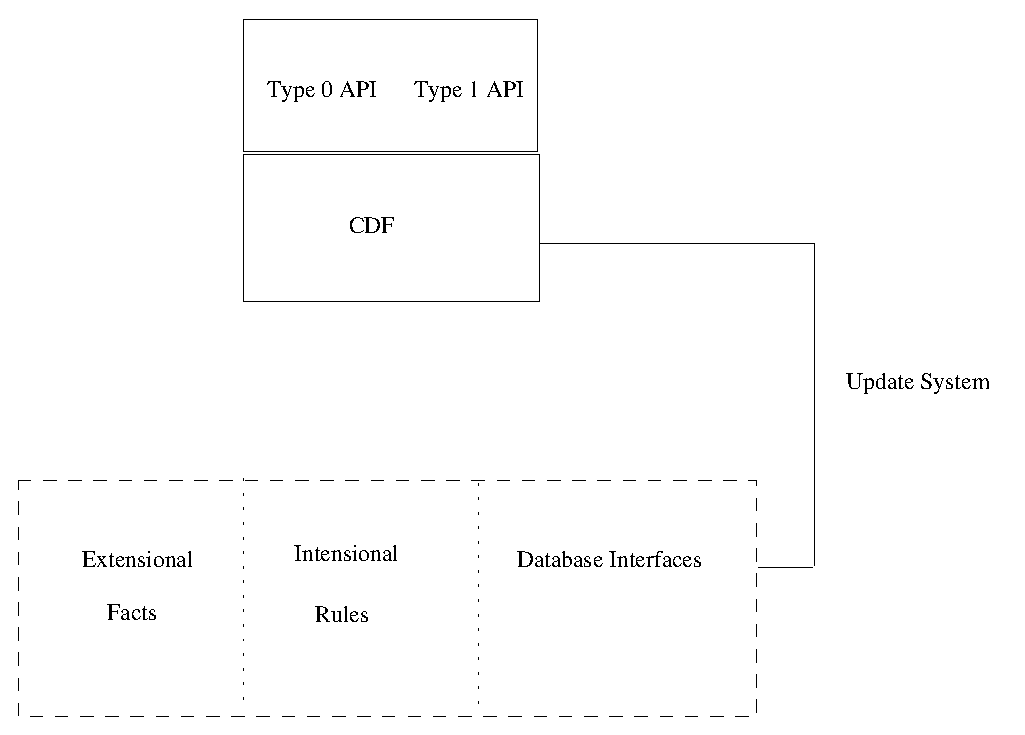
\epsfig{file=Figures/arch.eps,width=0.80\textwidth}}
%\caption{A High-Level Architecture of CDF and XJ}
%\label{fig:arch}
%\end{figure}
%--------------

CDF instances can be classified either as Type-0 or a Type-1, each of
which has its own interface.  Type-0 instances are useful for storing
large amounts of information; and consistency and implication in
Type-0 instances is computable in polynomial time.  Type-0 instances
describe classes by existential and universal relations, qualified
number restrictions, and relational hierarchies, but descriptions omit
negation and disjunction. Type-0 instances also support a direct
product construction for objects and classes.  
\comment{
These product classes and objects can be useful for representing
certain types of non-binary relations, and are particularly useful for
incorporating knowledge represented as RDF facts \cite{}.  }
Information in Type-0 CDF instances is tightly coupled to XSB's
query mechanism, and CDF ensures that only the most specific answers
(according to a given inheritance hierarchy) are returned for any
Type-0 query.

Type-1 instances extend Type-0 instances to describe classes using
negation and disjunction, and thus permit descriptions that are
equivalent to an expressive description logic.  In fact, a Type-1 CDF
instance can be seen as a knowledge base in which various classes are
described via {\em class expressions}, which correspond to formulas in
description logics.  Reasoning in Type-1 instances is done via the CDF
theorem-prover.  Using the Type-1 API, users may ask whether a given
class or object is consistent, whether a given class expression is
consistent with a class or object; or whether a given class expression
is entailed by a given class or object.  The problems of determining
consistency or entailment of a Type-1 class expression have a high
degree of complexity.  To solve these problems the CDF theorem prover
uses several heuristics, but a determined (or unlucky) user can always
find class expressions that requires a lot of time to check.

Of course, ontology management systems require many features in
addition to reasoning and representation features \cite{MGPS03}.  We
mention some of these features.

\begin{itemize}
\item {\em A Semantic Checking System}.  CDF has various mechanisms for
ensuring consistency of objects and classes both at the Type-0 or
Type-1 level.  Various levels of consistency can be checked during
various operations on the CDF instance.
%
\item {\em A Component System}. Reusability of ontologies is supported
by the {\em component} structure of CDF.  An ontology component may be
maintained by separate users or organizations in different locations
and assembled in various ways by applications.
%
\item {\em A Concurrency System}. (Not open-source) Based on the
component structure, the {\em concurrency} mechanism for CDF allows
users to update their own CDF instances and to periodically update a
common store. Naturally, the various mechanisms in CDF for ensuring
consistency that are vital to ensuring coherency when users update
their systems concurrently.
%
\item {\em Database Interfaces}. (Non open-souce) CDF supports various
interfaces to databases so that CDF facts can be stored in a database
or mapped to database tables.
\end{itemize}

Based on these features, CDF can support user interfaces in a number
of ways.  One of the most convenient is to use a XSB/Java interface
such as InterProlog~\cite{Cale01} or JAXSB~(see
\texttt{http://xsb.sourceforge.net}) and then write a user interface in
Swing or some other Java Graphics library.  One of the easiest ways to
do this is to make use of the {\em XJ system} which allows Swing Gui
objects to be represented as Prolog terms (the XJ system is non
open-source) From a systems perspective, a graphical interface is then
written XJ library Swing widgets or specialized XJ-CDF Swing widgets.
CDF per-se has the following graphical packages and applications.
%
\begin{itemize}
%
\item {\em An XJ Caching System}. Adds and deletes to CDF are extended
with a notification mechanism so that Java Swing objects (created with
XJ, XSB's graphics system) reflect the state of CDF even when it
dynamically changes.
%
\item {\em A Visual Editor}. Finally,  CDF supports a graphical editor
that allows users both to visualize an ontology and to perform the
functions mentioned so far.
\end{itemize}
%
Extensional facts, intensional rules, updates, the Type-0 and Type-1
interfaces, consistency checking predicates and the full component
system are available as an open-source package for XSB.  Other
features, concurrency mechanisms, specialized database interfaces, XJ
support and the editor are not yet open-source, but are included in
this manual to indicate the types of applications that can be
constructed with CDF.

%-----------------------------------------------------------
\section{The Meaning of Type-0 CDF Instances} \label{sec:type0} 

Facts in both Type-0 and Type-1 CDF instances are closely related to
class expressions in description logics.  However, because CDF often
stores class expressions as Prolog facts in an unconventional way, and
because description logics may not be familiar to a logic programming
audience, we present here a somewhat formal introduction to how CDF
represents knowledge.  Users without a mathematical background can
ignore the various axioms and formal definitions that are presented in
this chapter.  Our approach is to introduce a semantics of CDF based
on a translation of a {\em CDF instance} into a set of first-order
logic sentences that constitute an {\em Ontology Theory} whose models
are the models of a CDF instance.  For simplicity of presentation the
description of CDF instances in this section omits certain details
about components, extensional facts and intenstional rules, and other
topics that will be introduced in later chapters.

We illustrate aspects of CDF by means of an example drawn from
electronic commerce.  Health care organizations, such as hospitals,
clinics, etc., sometimes have difficulties in buying disposable
medical devices such as sutures, bandages, gloves, and so on.  These
difficulties arise from the fact that these devices may be quite
specialized: for instance some sutures are used only for particular
type of surgery on a particular organ.  At the same time, since these
devices are disposable, they may need to be purchased frequently.  We
consider concretely the class of {\em absorbable sutures}, which are
used for stitching and securing tissues, and which can be absorbed by
the human body.  Information below is adapted from he U.S. Defence
Logistics Information Service \url{http://www.dlis.mil}, from the
Universal Standard Products and Services Classification~\cite{UNSPSC},
as well as from websites of various commercial medical supply
companies.

\subsection{Type-0 CDF Instances} \label{sec:type0} 

We begin with the syntax of Type-0 instances~\footnote{The syntax for
  identfiers is simplified here, and differs in the actual CDF
  implementation. See Section~\ref{sec:instance}.}:

\begin{definition}[Type-0 Instances: Semantic Level] \label{def:ids}
A {\em Type-0 CDF instance} is a finite set of ground facts for the
predicates \pred{isa/2}, \pred{hasAttr/3}, \pred{allAttr/3},
\pred{classHasAttr/3}, \pred{minAttr/4}, and \pred{maxAttr/4}.  An {\em
identifier} is either a constant or a term.  The arguments of these
predicates are {\em concrete identifiers}, where a term $T$ is an
identifier iff $T$ has the functor symbol {\tt cid/1}, {\tt oid/1},
{\tt rid/1}, or {\tt crid/1} whose argument is either

\begin{enumerate}
\item a constant; or 
\item a term $f(I_1,\ldots,I_n)$ where $I_1,\ldots,I_n$ are identifiers.
\end{enumerate}
In the first case, an identifier is called {\em atomic}; in the second
it is called a {\em product identifier}.
\end{definition}

Despite the simple syntax of Type-0 CDF instances, their semantics
differs from the usual semantics assigned to facts in Prolog.
Identifiers identify sets of objects, or binary relations between
objects.  Furthermore, the facts of a Type-0 CDF instance can
implicitly denote inheritance of various relationships among classes
and objects, as well as inheritance constraints about what
relationships are allowed.

\subsection{Simple Taxonomies in CDF}

\begin{example} \rm \label{ex:suture1}
The following CDF instance illustrates a fragment of a taxonomy for
medical equipment.
%-------------------------------------------
{\tt  {\small 
\begin{tabbing}
foo\=foo\=foo\=foo\=foo\=foo\=foooo\=foooooooooooooooo\=\kill
isa(cid(medicalEquipment),cid('CDF Classes'))  \\
\> isa(cid(woundCareProducts),cid(medicalEquipment)) \\
\> \> \>  isa(cid(suturesAndRelatedProducts),cid(woundCareProducts)) \\
\> \> \> isa(cid(sutures),cid(suturesAndRelatedProducts))  \\
\> \> \> \> isa(cid(absorbableSutures),cid(sutures))  \\
\> \> \> \> isa(cid(nonAbsorbableSutures),cid(sutures)) \\
\> \\
\> \> \>   isa(oid(sutureU245H),cid(absorbableSutures))  \\
\> \> \> \> \>   isa(oid(suture547466),cid(sutures)) 
\end{tabbing} }} 
%-------------------------------------------
\noindent
In CDF, sets of objects are termed {\em classes} to stress the
informality of its sets from the perspective of set theory, and class
identifiers have the functor {\tt cid/1}.  One can read the fact
\begin{verbatim}
      isa(cid(nonAbsorbableSutures),cid(sutures))
\end{verbatim}
as ``all elements in the class {\tt cid(nonAbsorbableSutures)} are
also in the class {\tt cid(sutures)}'' --- in other words, that {\tt
cid(nonAbsorbableSutures)} is a subclass of {\tt cid(sutures)}.
Object identifiers have the functor {\tt oid/1}, and denote classes
with cardinality 1, or {\em singleton classes}.  The fact
\begin{verbatim}
      isa(oid(sutureU245H),cid(absorbableSutures))
\end{verbatim}
can be read as ``the element of the singleton class {\tt
oid(sutureU245H)} is in the class {\tt cid(absorbableSutures)}''.
Note that {\tt cid(absorbableSutures)} is (potentially) more specific
than the class {\tt cid(sutures)}, to which {\tt oid(suture547466)}
belongs.  The class {\tt cid('CDF Classes')} is taken to contain all
objects in the domain of discourse.  All identifiers in this simple
taxonomy are atomic.

The decision of whether to denote an entity as an object or as a class
depends on the use of a given CDF instance.  Here, a given part number
can specify a number of physical parts, but the physical parts are
taken to be identical for the purposes of this instance.  However, if
we were constructing a CDF instance for warehouse management, the
above objects might be better represented as classes, and the physical
objects represented as CDF objects.
\end{example} 

Implicit in the above example is the fact that we use the term {\em
object identifiers} or {\em objects} to denote singleton classes,
class identifiers to denote all classes (including singleton classes).
Elements cannot be denoted directly by CDF facts, but only through
singleton classes that contain them (and are isomorphic to them).  At
this point, we can begin defining the semantics of Type-0 CDF
instances.

%-------------------
\begin{definition} \label{def:ontolang}
\index{ontology language} \index{ontology structure} \index{ontology
theory}
%
An {\em ontology language} is a first-order language with equality
containing the predicates: {\em isClass/1, isElt/1, isRel/1, isCrel/1,
elt/2, rel/3, and crel/3}, and a countable set of constants.  An {\em
ontology structure} is a structure defined over an ontology language.
An {\em ontology theory} is a set of first-order sentences formed over
an ontology language that includes a set of {\em core axioms}, defined
below, along with the defined predicate:
\[
isObj(X) =_{def} isClass(X) \wedge 
	((elt(E_1,X) \wedge elt(E_2,X)) \Rightarrow E_1 = E_2)
\]
If $\cT$ is an ontology theory formed over an ontology
language $\cL$, an ontology structure $S$ over $\cL$ is a model of
$\cT$ if every sentence of $\cT$ is satisfied in $S$.
\end{definition}
%-------------------

\index{sorting predicates}
By convention we assume that the variables in an ontology language are
indexed by the set of natural numbers.  In this paper we will restrict
our attention to ontology languages whose constant and function
symbols are identifiers as described in Definition~\ref{def:ids}.
Informally $isClass/1$ indicates that an identifier $I$ is a class
name or {\em class identifier}; $isElt/1$ indicates that an identifier
$I$ is an element of a class; $isRel/1$ that $I$ is a {\em relation
identifier}; and $isCrel/1$ that $I$ is a {\em class-relation
identifier}; and $isObj/1$ that $I$ is an {\em object identifier}.  We
sometimes call these 5 predicates {\em sorting predicates}.
$elt(E,C)$ indicates that an element $O$ is a member of class
identifier $C$; $rel(O_1,R,O_2)$ indicates that an element $E_1$ has a
$R$ relation to an element $E_2$; and $crel(C_1,R,E)$ indicates that
the class identifier $C_1$ has a $R$ relation to an object identifier
$E$.

The first core axiom ensures that objects, classes, relations and
class-relations all have distinct identifiers within an ontology
language.
%-----------
\begin{axiom}[Distinct Identifiers] \label{ax:distinct}
\index{axioms!distinct identifiers} 
\ \\
\begin{tabbing}
foo\=foo\=foo\=foo\=foo\=foo\=foooo\=foooooooooooooooo\=\kill
\> $\neg \exists Id [isClass(Id) \wedge (isElt(Id) \vee isRel(Id) 
	                                 \vee isCrel(Id))] \wedge $ \\
\> $\neg \exists Id [isObj(Id) \wedge (isElt(Id) \vee isCrel(Id))] \wedge $ \\
\> $\neg \exists Id [isElt(Id) \wedge isCrel(Id)] $ 
\end{tabbing}
\end{axiom} 
%-----------

$isClass/1$, $isElt/1$, $isRel/1$, and $isCrel/1$ provide an effective
sorting that extends to all predicates, as the next axiom indicates.

\begin{axiom}[Predicate Sorts] \rm \label{ax:sorts}
\index{axioms!predicate sorts} 
\ \\
\begin{tabbing}
foo\=foo\=foo\=foo\=foo\=foo\=foooo\=foooooooooooooooo\=\kill
\> \> $(\forall X,Y) [elt(X,Y) \Rightarrow (isElt(X) \wedge isClass(Y))]
								\wedge $ \\
\> \> $(\forall X,Y,Z) [rel(X,Y,Z) \Rightarrow (isElt(X) \wedge isRel(Y)
					   \wedge isElt(Z))] \wedge  $ \\
\> \> $(\forall X,Y,Z) [crel(X,Y,Z) \Rightarrow (isClass(X) \wedge isRel(Y)
					   \wedge isElt(Z))] $ \\
\end{tabbing}
\end{axiom} 

%-----------

The following definition of $IdSort$ relates the functors of
identifiers in a Type-0 CDF instance to their sort in an ontology
theory.  It will be used in the various instance axioms to enforce
proper sorting of product identifiers.

\begin{definition}{\bf [IdSort]} \label{def:IdSort}
Let {\em I} is be an identifier. Then {\em IdSort(I)} is equal to {\em
isClass(I)} if the main functor symbol of {\em I} is {\tt cid/1}; {\em
isObj(I)} if the main functor symbol of {\em I} is {\tt oid/1}; {\em
isRel(I)} if the main functor symbol of {\em I} is {\tt rid/1}; and
{\em isCrel(I)} if the main functor symbol of {\em I} is {\tt crid/1}.
\end{definition}

%-----------------------------------------------------------------------------------------
\comment{
\begin{definition}{\bf [IdSort]}  Let {\em I} is be an identifier, and
$\cI$ be the set of identifiers occurring in {\em I}. Then
%
\[ IdSort(I) =_{def} \bigwedge_{I' \in \cI} Sort(I') \]
%
where {\em Sort(I)} is equal to {\em isClass(I)} if the main functor
symbol of {\em I} is {\tt cid/1}; {\em isObj(I)} if the main functor
symbol of {\em I} is {\tt oid/1}; {\em isRel(I)} if the main functor
symbol of {\em I} is {\tt rid/1}; and {\em isCrel(I)} if the main
functor symbol of {\em I} is {\tt crid/1}.
\end{definition}
}
%-----------------------------------------------------------------------------------------

From Definitions~\ref{def:IdSort} and~\ref{def:ontolang}, it is easy
to see that for any object identifier $O$, $IdSort(O) = isObj(O)$, and
$isObj(O) \Rightarrow isClass(O)$.

%-----------
\begin{instance} [Translation of {\tt isa/2}] \rm 
For each fact of the form {\tt isa(Id$_1$,Id$_2$)} add the axiom
\ \\
\begin{tabbing}
foo\=foo\=foo\=foo\=foo\=foo\=foooo\=foooooooooooooooo\=\kill
\> $ IdSort(Id_1) \wedge IdSort(Id_2) \wedge $ \\

\> \> $ (((isClass(Id_1) \wedge isClass(Id_2)) \wedge
	(\forall X) [elt(X,Id_1) \Rightarrow elt(X,Id_2)]) \vee $ \\

%\> \> $ ((isObj(Id_1) \wedge isClass(Id_2)) \wedge elt(Id_1,Id_2)) \vee $ \\

\> \> $ ((isRel(Id_1) \wedge isRel(Id_2)) \wedge
	(\forall X,Y)[rel(X,Id_1,Y) \Rightarrow rel(X,Id_2,Y)]) \vee $ \\

\> \> $ ((isCrel(Id_1) \wedge isCrel(Id_2)) \wedge
	(\forall X,Y)[crel(X,Id_1,Y) \Rightarrow crel(X,Id_2,Y)])) $ 
\end{tabbing}
denoted as {\tt isa(Id$_1$,Id$_2$)}$^{\cI}$.
\end{instance}
%-----------

Note that the reflexive and transitive closure of {\tt isa/2} is an
immediate consequence of its translation rule.  The next axiom is
technical.  It is important for the semantics of relations that each
class have at least one member.
%-----------
\begin{axiom}[Non-Empty Classes] \label{ax:nonnull}
\index{axioms!non-empty classes} 
\[ (\forall X) [isClass(X) \Rightarrow (\exists Y) [elt(Y,X)]] \]
\end{axiom} 
%-----------

The last core axiom for these predicates ensures is that each class is
a subclass of {\tt cid('CDF Classes')}.

%-----------
\begin{axiom}[Domain Containment] \label{ax:contained}
\index{axioms!domain containment} 
\[ (\forall X) [isElt(X) \Rightarrow elt(X,cid('CDF\ Classes'))] \]
\end{axiom} 
%-----------

\subsection{General Relations between Objects in  Classes}

\begin{example} \rm \label{ex:suture2}
The class {\tt cid(sutures)} can be further defined by its relations
to other classes.  For instance, an object in {\tt cid(sutures)} may
have a designation of its needle design indicating whether it is to be
used for abdominal surgeries, thoracic surgeries, or other purposes.
This information is indicated by the following CDF facts:
%
{\small
\begin{tabbing}
fooo\=foo\=foo\=foo\=fooooooooooooooooooooooooooooooo\=ooooooooooooo\=\kill
\> {\tt isa(rid(hasNeedleDesign),rid('CDF Relations'))} \\
\\
\> {\tt isa(cid(domainTypes),cid('CDF Classes'))} \\
\> \> {\tt isa(cid(needleDesignTypes),cid(domainTypes))} \\
\> \> \> {\tt isa(cid(Abdominal),cid(needleDesign))} \\
\> \> \> {\tt isa(cid(Abscisson),cid(needleDesign))} \\
\> \> \> {\tt isa(cid('Adson Dura'),cid(needleDesign))} \\
\> {\it \% 126 other values..}  \\
\\
\> {\tt allAttr(cid(sutures),rid(hasNeedleDesign),cid(needleDesign))} 
\end{tabbing}
}
%
\noindent
The {\tt allAttr/3} fact above can be read as ``if any object in {\tt
cid(absorbableSutures)} has a {\tt rid(hasNeedleDesign)} relation, it
must be to an object in the class {\tt cid(needleDesign)}''.  That
{\tt hasNeedleDesign} is a relation is indicated by clothing it in the
functor {\tt rid/1}.  This relation is an immediate subclass of all
{\tt CDF Relations} which in turn is taken to represent the universal
binary relation over the domain of discourse.  Thus the {\tt
allAttr/3} fact effectively types the range of {\tt
rid(hasNeedleDesign)} relations, stemming from objects in the class
{\tt cid(absorbableSutures)}, but it does not indicate the existence
of such a relationship.  From a user's point of view, the {\tt
rid(hasNeedleDesign)} relation can be thought of as an optional
attribute for a given {\tt cid(absorbableSutures)} object.  Sample
values for {\tt cid(hasNeedleDesignTypes)} are also given.
\end{example} 

%-------------------

{\tt allAttr/3} provides a simple but powerful mechanism for
inheritance of typing among CDF classes:
%---------------------------------------------------------------------------
\comment{
, as can be seen from the
following translation rule, which uses the defined formula

\[ 
elt(X,Y) =_{def} ((isClass(Y) \wedge elt(X,Y)) \vee (isObj(Y) 
			\wedge X = Y))
\] }
%---------------------------------------------------------------------------

\begin{instance} [Translation of {\tt allAttr/3}] \rm 
For each fact of the form {\tt allAttr(Id$_1$,Rid,Id$_2$)} add the instance
axiom: 
\begin{tabbing}
foo\=foo\=foo\=foo\=foo\=foo\=foooo\=foooooooooooooooo\=\kill
\> $ IdSort(Id_1) \wedge IdSort(Rid) \wedge IdSort(Id_2) \wedge $ \\
\> \> $ IsClass(Id_1) \wedge IsRel(Rid) \wedge IsClass(Id_2) \wedge $ \\
\> \> $(\forall X, Y) [(elt(X,Id_1) \wedge rel(X,Rid,Y))
					\Rightarrow elt(Y,Id_2)] $
\end{tabbing}
denoted as {\tt allAttr(Id$_1$,Rid,Id$_2$)$^{\cI}$}.
\end{instance}

%----------------------
\comment{
\begin{tabbing}
foo\=foo\=foo\=foo\=foo\=foo\=foooo\=foooooooooooooooo\=\kill
\> $ IdSort(Id_1) \wedge IdSort(Rid) \wedge IdSort(Id_2) \wedge $ \\
\> \> $ (IsClass(Id_1) \vee isObj(Id_1)) \wedge IsRel(Rid) \wedge 
	 (IsClass(Id_2) \vee isObj(Id_2)) \wedge $ \\
\> \> $(\forall X, Y) [(elt(X,Id_1) \wedge rel(X,Rid,Y))
					\Rightarrow elt(Y,Id_2)] $
\end{tabbing}
}
%----------------------
\begin{example} \rm \label{ex:hasAttr}
While {\tt allAttr/3} indicates a typing for relations, it does not
indicate that a relation must exist for elements of a class.  This
statement is made by \pred{hasAttr/3}.  The relation {\tt
rid(hasPointStyle)} for the class {\tt cid(absorbableSutures)} is
taken to be required in this schema.  The facts
%
{\small
\begin{tabbing}
fooo\=foo\=foo\=foo\=foooooooooooooooooooooooooooo\=ooooooooooooo\=\kill
\> {\tt allAttr(cid(absorbableSutures),rid(hasPointStyle),cid(pointStyle)) } \\
\> {\tt hasAttr(cid(absorbableSutures),rid(hasPointStyle),cid(pointStyle)) }
\end{tabbing}
}
%
\noindent
indicate not only the range of such relationships, but that such a
relationship must exist.  Indeed, the {\tt hasAttr/3} fact can be read
as ``all objects in the class {\tt cid(absorbableSutures)} have a
relation {\tt rid(hasPointStyle)} to an object in the class {\tt
cid(pointStyle)}''.  The facts below also give information about the
{\tt rid(hasPointStyle)} relation.
%
{\small
\begin{tabbing}
fooo\=foo\=foo\=foo\=foooooooooooboooooooooooooooo\=ooooooooooooo\=\kill
\> {\tt isa(cid(pointStyle),cid(domainTypes))} \\
\> {\tt isa(cid(regularCuttingEdge),cid(pointStyle))} \\
\> {\tt isa(cid(reverseCuttingEdge),cid(pointStyle))} \\
\> {\tt isa(cid(scalpelPoint),cid(pointStyle))} \\
\> {\it \% 10 other values.} \\
\\
\> {\tt hasAttr(oid(sutureU245H),rid(hasPointStyle),cid(regularCuttingEdge))}
\end{tabbing}
} 
\noindent
The last of the above facts can be read as ``the object {\tt
oid(sutureU245H)} has a {\tt rid(hasPointStyle)} relation to an object
in the class {\tt cid(pointStyle)}''.  
\end{example}

Not surprisingly, the definition of {\tt hasAttr/3} bears some
similarity to that of {\tt allAttr/3}.

\begin{instance} [Translation of \pred{hasAttr/3}] \rm 
For each fact of the form {\tt hasAttr(Id$_1$,Rid,Id$_2$)} add the instance
axiom: 
\begin{tabbing}
foo\=foo\=foo\=foo\=foo\=foo\=foooo\=foooooooooooooooo\=\kill
\> $ IdSort(Id_1) \wedge IdSort(Id_2) \wedge IdSort(Id_2) \wedge $ \\
\> \> $ IsClass(Id_1) \wedge IsRel(Rid) \wedge
	 IsClass(Id_2) \wedge $ \\
\> \> \> $ (\forall X) [elt(X,Id_1) \Rightarrow \exists Y [rel(X,Rid,Y) 
					\wedge elt(Y,Id_2)]]$
\end{tabbing}
denoted as {\tt hasAttr(Id$_1$,Rid,Id$_2$)$^{\cI}$}.
\end{instance}

We next turn to relational axioms that indicate the cardinality of
various relations.

\begin{example} \rm  \label{ex:maxAttr}
For our purposes, an object in {\tt cid(absorbableSutures)} can be
thought of as consisting of a needle and a thread~\footnote{The thread
is often called a suture.  We are assuming for purposes of
illustration that all sutures are --- in suture-speak --- ``armed''.}.  This is
represented by the facts:
%
{\small
\begin{tabbing}
foo\=foo\=foo\=foo\=foo\=foo\=foooo\=foooooooooooooooo\=\kill
\> {\tt allAttr(cid(absorbableSutures),rid(hasImmedPart),cid(absSutPart)) } \\
\> {\tt hasAttr(cid(absorbableSutures),rid(hasImmedPart),cid(absSutNeedle)) } \\
\> {\tt hasAttr(cid(absorbableSutures),rid(hasImmedPart),cid(absSutThread)) } \\
\\
\> {\tt isa(cid(absSutPart),cid(suturesAndRelatedProducts))}  \\
\> \> {\tt isa(cid(absSutNeedle),cid(absSutPart)) } \\
\> \> {\tt isa(cid(absSutSuture),cid(absSutPart)) } 
\end{tabbing}
}
%
\noindent
A needle for an absorbable suture is typically made of a different
material than the thread to which the needle is attached.  Each of
these materials may be important in choosing an absorbable suture, and
each of these materials are unique.  The facts
%
{\small
\begin{tabbing}
foo\=foo\=foo\=foo\=foo\=foo\=foooo\=foooooooooooooooo\=\kill
\> {\tt hasAttr(cid(absSutPart),rid(hasMaterial),cid(absSutMaterial)) } \\
\> {\tt maxAttr(cid(absSutPart),rid(hasMaterial),cid(absSutMaterial),1) } \\
\\
\> {\tt isa(cid(material),cid(domainTypes))} \\
\> {\tt isa(cid(absSutMaterial),cid(material)} \\
\> {\tt isa(cid(gut),cid(absSutMaterial))} \\
\> {\tt isa(cid(polyglyconate),cid(absSutMaterial))} \\
\> {\tt isa(cid(polyglyconicAcid),cid(absSutMaterial)) } 
\end{tabbing}
}
%
\noindent
indicate that each {\tt cid(absSutPart)} has a unique material.  The
{\tt maxAttr/4} fact can be read as ``Each object in the class {\tt
cid(absSutPart)} has at most 1 {\tt rid(hasMaterial)} relation to an
object in the class {\tt cid(absSutMaterial)}''.
\end{example}

In order to define the semantics of {\tt maxAttr/4}, let
$\exists^{\leq n}X_m[ \phi(X,Z)]$ be defined as an abbreviation for
the formula
\[
  \exists x_m,...,\exists x_{m+n} [\bigwedge_{m \leq i \leq m+n} 
	\phi(x_i,\overline{z}) 
	\Rightarrow \bigvee_{m \leq i < j \leq m+n} x_i  = x_j]
\]
i.e., for the formula indicating that there are at most $N$ non-equal
elements satisfying $\phi(x,z)$.  The abbreviation $\exists^{\geq N}$
is defined similarly to indicate that a formula is satisfied by at
least $N$ non-equal elements.

\begin{instance} [Translation of {\tt maxAttr/4}] \rm 
For each fact of the form {\tt maxAttr(Id$_1$,Rid,Id$_2$,N)} add the instance
axiom: 
\begin{tabbing}
foo\=foo\=foo\=foo\=foo\=foo\=foooo\=foooooooooooooooo\=\kill
\> $ IdSort(Id_1) \wedge IdSort(Id_2) \wedge IdSort(Id_2) \wedge $ \\
\> \> $ IsClass(Id_1) \wedge IsRel(Rid) \wedge
	 (IsClass(Id_2) \wedge $ \\
\> \> \> $ (\forall X) [elt(X,Id_1) \Rightarrow \exists^{\leq N} Y [rel(X,Rid,Y) 
					\wedge elt(Y,Id_2)]]$
\end{tabbing}
denoted as {\tt maxAttr(Id$_1$,Rid,Id$_2$,N)$^{\cI}$}.
\end{instance}

A corresponding predicate, {\tt minAttr/4} is used to indicate a
minimality restriction on a relation.  {\tt minAttr/4} is defined
similarly to {\tt maxAttr/4}, but using $\exists^{\geq N}$ rather than
$\exists^{\leq N}$.  Indeed, the predicate
%
{\small {\tt 
\begin{tabbing}
foo\=foo\=foo\=foo\=foo\=foo\=foooo\=foooooooooooooooo\=\kill
\> hasAttr(cid(absSutPart),rid(hasMaterial),cid(absSutMaterial)).
\end{tabbing}
} }
%
\noindent
could be replaced by the predicate
%
{\small {\tt 
\begin{tabbing}
foo\=foo\=foo\=foo\=foo\=foo\=foooo\=foooooooooooooooo\=\kill
\> minAttr(cid(absSutPart),rid(hasMaterial),cid(absSutMaterial),1).
\end{tabbing}
} }
%
\subsection{Class Relations}
Each of the predicates discussed so far are inheritable in their first
argument.  For instance, the fact
{\small {\tt 
\begin{tabbing}
foo\=foo\=foo\=foo\=foo\=foo\=foooo\=foooooooooooooooo\=\kill
\> hasAttr(cid(absSutPart),rid(hasMaterial),cid(absSutMaterial)).
\end{tabbing}
} } 
%
\noindent
implies that every subclass of {\tt cid(absSutures)} will have a
material in the class {\tt cid(absSutMaterial)}.  However, classes may
have relations that do {\em not} hold for their subclasses or members.
For instance, a finite set may have a given cardinality, but its
proper subsets will have a different cardinality.  Such relations are
termed {\em class relations}.

%-------------------
\begin{example} \label{ex:strel} \rm 
A practical example of a class relation comes from an application that
may be called part equivalency matching.  In this application, the
possible attributes for a class of parts are given various weights.
Two parts match if the sum of the weights of their attributes that
match are above a given threshold.  The weighting for the {\tt
cid(pointStyle)} of sutures might be given as:
%----------------------------------
{\small 
{\tt 
\begin{tabbing}
foo\=foo\=foo\=foo\=foo\=foo\=foooo\=foooooooooooooooo\=\kill
\> isa(cid(pointStyleWeight),cid('CDF Classes')) \\
\> \> isa(cid(highWeight),cid(pointStyleWeight)) \\
\> \> isa(cid(lowWeight),cid(pointStyleWeight)) \\
\\
\> classHasAttr(cid(sutures),crid(pointStyleWeight),cid(highWeight))
\end{tabbing}
} }
%----------------------------------
\noindent
The {\tt classHasAttr/3} fact can be read as ``the class {\tt
cid(sutures)} has a {\tt crid(pointStyleWeight)} relation to an object
in {\tt cid(highWeight)}.  Matching weights are made non-inheritable
via {\tt classHasAttr/3} because a weight may depend on a given
classification of a part.  For instance if a part were classified as a
{\tt cid(nonAbsorbableSuture)}, its {\tt cid(pointStyle)} might weigh
less (or more) for determining whether two sutures are equivalent.
\end{example}
%------------------
\begin{instance} [Translation of {\tt classHasAttr/3}] \rm 
For each fact of the form {\tt classHasAttr(Id$_1$,CRid,Id$_2$)} add the
instance axiom: 
\begin{tabbing}
foo\=foo\=foo\=foo\=foo\=foo\=foooo\=foooooooooooooooo\=\kill
\> $ IdSort(Id_1) \wedge IdSort(CRid) \wedge IdSort(Id_2) \wedge $ \\
\> \> $ IsClass(Id_1) \wedge IsCrel(CRid) \wedge isClass(Id_2) \wedge $ \\
\> \> \> $ (\exists X) [elt(X,Id_2) \wedge crel(Id_1,CRid,X)] $
\end{tabbing}
denoted as {\tt classHasAttr(Id$_1$,Rid,Id$_2$)$^{\cI}$}.
\end{instance}
%----------

\subsection{Product Classes}

The above predicates allow the definition of various named binary
relations between classes.  However, binary definitions can sometimes
be inconvenient to use.  For instance, in the part equivalency
matching example, (Example~\ref{ex:strel}), it may be desirable to
make explicit the weight of the match as an indication of the strength
of the match.  The weight could be made explicit by a series of
definitions
%-------------------------------------------
{\small 
{\tt 
\begin{tabbing}
foo\=foo\=foo\=foo\=foo\=foo\=foooo\=fooooooooooooooo\=\kill
\> allAttr(\cid{dlaPart},\rid{suturesRusMatch\_low},\cid{suturesRusPart}) \\
\> : \\
\> allAttr(\cid{dlaPart},\rid{suturesRusMatch\_high},\cid{suturesRusPart})
\end{tabbing}
} } 
%----------------------------------
\noindent
indicting that a given part has a match of weight {\em low} through
{\em high}.  However, for a scale with a large number of values,
defining matches in this way is time-consuming and prone to errors.
To address this, we first define a new class {\tt \cid{matchScale}}
containing as subclasses the various match levels.  We then combine
{\tt \cid{matchScale}} with the class {\tt \cid{suturesRusPart}} in a
product with a {\em product identifier}, as in the following fact
%-------------------------------------------
{\small 
{\tt 
\begin{tabbing}
foo\=foo\=foo\=foo\=foo\=foo\=foooo\=foooooooooooooooo\=\kill
 
allAttr(\cid{dlaPart},\rid{suturesRusMatch}, \\
\> \> \> \> \cid{partMach(\cid{suturesRusPart},\cid{matchScale})})
\end{tabbing}  } }
\noindent 
which indicates that a {\tt \cid{dlaPart}} can have a {\tt
\cid{suturesRusMatch}} to an object in the {\tt partMatch/2}  class,
which has both a {\tt \cid{suturesRusPart}} component and a {\tt
\cid{matchScale}} component.

%-------------------------------------------------------------------

We capture the intuition behind product classes through the following
axiom schemas.  The first indicates that product identifiers 
are constructed from {\em constituent identifiers} of the same sort.

\begin{axiom}[Downward Closure] \label{ax:downcl}
\index{axioms!downward closure}
\ \\
For each product identifier $\cid{f(x_1,\ldots,x_n)}$,
$\oid{f((x_1,\ldots,x_n)}$, $\rid{f(x_1,\ldots,x_n)}$, and
$c\rid{f((x_1,\ldots,x_n)}$ the following axiom is added,
\begin{tabbing}
foo\=foo\=foo\=foo\=foo\=foo\=foooo\=foooooooooooooooo\=\kill
\> $isClass(\cid{f(x_1,\ldots,x_n)}) \Rightarrow 
	isClass(x_1) \wedge \ldots \wedge isClass(x_n) $\\
\> $isObj(\oid{f(x_1,\ldots,x_n)}) \Rightarrow 
	isObj(x_1) \wedge \ldots \wedge isObj(x_n) $\\
\> $isRel(\rid{f(x_1,\ldots,x_n)}) \Rightarrow 
	isRel(x_1) \wedge \ldots \wedge isRel(x_n) $\\
\> $isCrel(\crid{f(x_1,\ldots,x_n)}) \Rightarrow 
	isCrel(x_1) \wedge \ldots \wedge isCrel(x_n) $
\end{tabbing}
\end{axiom}

With this axiom, along with the use of $IdType/1$ in the various
instance axioms, we will sometimes refer to a CDF identifier $I$ as a
class identifier if its outer functor is {\tt cid/1}, an object
identifier if its outer functor is {\tt oid/1} etc.  The next axiom
associates product classes with the objects they contain.

\begin{axiom}[Implicit Subclassing] \label{ax:implsc}
\index{axioms!implicit subclassing} 

\begin{enumerate}
\item For each product identifier $cid(f(x_1,\ldots,x_n))$ or 
$oid(f(x_1,...,x_n))$, the following axioms are added for $x_i, 1 \leq i
\leq n$:
\[
(\forall E) [(elt(E,y_i) \Ra elt(E,x_i)) \Ra \\
	(\forall E') [elt(E',f(x_1,...x_n))[x_i/y_i] \Rightarrow elt(E',f(x_1,...x_n))]]
\]

\item For each product identifier $rid(f(x_1,\ldots,x_n))$ the
following axioms are added for $x_i, 1 \leq i 
\leq n$:
\begin{tabbing}
foo\=foo\=foo\=foo\=foo\=foo\=foooo\=foooooooooooooooo\=\kill
\> $(\forall E_1,E_2) [(rel(E_1,y_i,E_2) \Ra rel(E_1,x_i,E_2)) \Ra$ \\
\> \> $(\forall E'_1,E'_2) [rel(E'_1,f(x_1,...x_n),E'_2)[x_i/y_i] \Ra rel(E'_1,f(x_1,...x_n),E'_2)]]$
\end{tabbing}
\end{enumerate}
\end{axiom}

%-------------------------------------------
\comment{
\begin{axiom}[Implicit Subclassing] \label{ax:implsc}
\begin{enumerate}
\item For each product identifier $\oid{f(x_1,\ldots,x_n)}$ the
following axiom is added:  
\[(\forall O) [elt(O,\cid{f(x_1,\ldots,x_n)})
	\Ra (O = \oid{f(y_1,\ldots,y_n)} \wedge 
  		  elt(y_1,x_1) \wedge \ldots \wedge elt(y_n,x_n))] \]

\item For each product identifier $\cid{f(x_1,\ldots,x_n)}$ and for
each atomic identifier $\cid{c}$ the following axiom is
added:
\[ (\forall C) 
   ([elt(\oid{f(x_1,\ldots,x_n)},C)] \Ra (C = \cid{f(y_1,\ldots,y_n)}
   \vee C = \cid{c})) \]
\end{enumerate}
\end{axiom}
}
%-------------------------------------------

\begin{example} \rm
Axiom~\ref{ax:downcl} simply states that identifier types cannot be
mixed within a product identifier.  For instance, if {\tt
\oid{matchLevelN}} is an object in the {\tt \cid{matchScale}},
then the identifier 

{\tt \cid{partMatch(\cid{suturesRusMatch},\oid{matchLevelN})}}

\noindent
is improperly formed.  On the other hand, if {\tt \oid{sutureU245H}} is in
the class {\tt \cid{suturesRusPart}}, then the identifier {\tt
\oid{partMatch(\oid{sutureU245H},\oid{matchLevelN})}} is a product
identifier that is also an object identifier.

Axiom~\ref{ax:implsc} also means that the inheritance relation of a
product class is partly determined by the inheritance relation of its
constituent elements.
\end{example}

\comment{
Core Axiom~\ref{ax:implsc} can be used either to set up equality
constraints on a model of a CDF instance, or it can be used to
determine which CDF instances have free models (as explained in the
next section).  The following example illustrates the first use.

\begin{example} \rm \label{ex:equality}
Suppose we have the CDF instance
{\small 
{\tt 
\begin{tabbing}
foo\=foo\=foo\=foo\=foo\=foo\=foooo\=foooooooooooooooo\=\kill
\> isa(\cid{a},\cid{f(a)}.
\end{tabbing} } } 
\noindent
By Core Axiom~\ref{ax:nonnull} (Non-empty Classes), {\tt \cid{a}} has
at least one element, which can be called {\tt \oid{a1}}.  By the
instance axiom for the above fact, {\em elt(\oid{a1},\cid{f(a)}}.  By
Core Axiom~\ref{ax:implsc}(1), it must be the case that 
%
\[ \oid{a1} = \oid{f(Y)} \wedge elt(Y,\cid{a}) \]
%
If we take $Y = \oid{a1}$, then this means that 
%
$ \oid{a1} = \oid{f(\oid{a1})} $
% 
so that the above fragment has a model $\cM$ with a single individual
(in the universe of $\cM$) to which all object identifiers are mapped,
and that has a $elt/2$ relation to each individual to which a class
identifier is mapped (among other models).
\end{example}
}

%\input{models}

\section{Implementation and System Features} \label{sec:impl}
%
In this section we describe how the CDF system implements the
semantincs of Section~\ref{sec:type0} , as well as many other features
for ontology management.  We begin by describing CDF identifiers,
facts, and rules in Section~\ref{sec:instance}.  The Type-0 query
interface, based on tabled resolution is described in
Section~\ref{sec:type0query}.  Section~\ref{sec:type0query} describes
the Type-1 API, which is based on the CDF therorem prover.  Update and
consistency predicates for CDF are described in
Section~\ref{sec:update}.  Section~\ref{sec:config} describes how to
configure CDF, along with predicates that allow the user to examine
aspects of the CDF state.  Section~\ref{sec:components} describes
basic I/O for CDF, along with a more sophisticated {\em component}
system that is built on top of basic I/O.  Section~\ref{sec:database}
describes database interfaces for CDF, and
Section~\ref{sec:concurrency} describes concurrency support.

%----------------------------------------------------


\subsection{CDF Instances} \label{sec:instance}

Part~\ref{part:semantics} simplified the syntax of CDF instances in
certain ways.  In this section we describe those aspects of the actual
CDF implementation that differ from the abstract presentation
Part~\ref{part:semantics}.

The first major difference concerns CDF identifiers.

\index{CDF Identifer}
\index{component tag}
\begin{definition}[CDF Identifiers] \label{def:cdfids}
A {\em CDF identifier} has the functor symbol {\tt cid/2}, {\tt
oid/2}, {\tt rid/2}, or {\tt crid/2}.  The second argument of a CDF
identifier is a Prolog atom and is called its {\em component tag},
while the first argument is either
\begin{enumerate}
\item a Prolog atom or 
\item a term $f(I_1,\ldots,I_n)$ where $I_1,\ldots,I_n$ are CDF identifiers.
\end{enumerate}
In the first case, an identifier is called {\em atomic}; in the second
it is called a {\em product identifier}.
\end{definition}

Thus in an implementation of, say, Example~\ref{ex:suture1} all
identifiers would have component tags.  For instance the identifier
{\tt cid(absorbableSutures)} might actually have the form {\tt
cid(absorbableSutures,unspsc)} and {\tt oid(sutureU245H)} would have
the form {\tt oid(sutureU245H,sutureRus)}.  These component tags have
two main uses.  First, they allow ontolgies from separate soruces to
be combined, and thus function in a manner somewhat analogous to XML
namespaces.  Second, the component tags are critical to the CDF
component system, described in \secref{sec:components}.

%----------------------------------------------------------------------------
\subsubsection{Extensional Facts and Intensional Rules}

\index{extensional facts} \index{intensional rules}
%
An actual CDF instance is built up of {\em extensional facts} and {\em
intensional rules} defined for the CDF predicates {\tt isa/2} {\tt
allAttr/3}, {\tt hasAttr/3}, {\tt classHasAttr/3}, {\tt coversAttr/3},
{\tt minAttr/4} and {\tt maxAttr/4}.  Extensional facts for these
predicates add the suffix {\tt \_ext} to the suffix name leading to
{\tt isa\_ext/2}, {\tt allAttr\_ext/2} and so on.  Intensional rules
add the suffix {\tt \_int} leading to {\tt isa\_int/2}, {\tt
allAttr\_int/2} etc.

Extensional facts make use of XSB's sophisticated indexing of dynamic
predicates.  Since CDF Extensional Facts use functors such as {\tt
  cid/1} or {\tt oid/1} to type their arguments, traditional Prolog
indexing, which makes use only of the predicate name and outer functor
of the first argument, is unsuitable for large CDF instances.  CDF
extensional facts use XSB's star-indexing (cf. Volume 1 of this
manual).  For ground terms, star-indexing can index on up to the first
five positions of a specified argument.  In addition, various
arguments and combinations of arguments can be used with star-indexing
of dynamic predicates.  The ability to index within a term is critical
for the performance of CDF; also since star-indexing bears
similarities to XSB's trie-indexing~\cite{RRSSW98}, it is spatially
efficient enough for large-scale use.  Section~\ref{sec:config}
provides information on default indexing in CDF and how it may be
reconfigured.

Intensional rules may be defined as XSB rules, and may use any of
XSB's language or library features, including tabling, database, and
internet access.  Intensional rules are called on demand, making them
suitable for implementing functionality from lazy database access
routines to definitions of primitive types.

\begin{example} \rm \label{ex:intrules}
In many ontology management systems, integers, floats, strings and so
on are not stored explicitly as classes, but are maintained as a sort
of {\em primitive type}.  In CDF, primitive types are easily
implemented via intensional rules like the following.
%
{\small {\sf  
\begin{tabbing}
foo\=foo\=foooooooooooooooooooooooooooooooooooooooo\=foo\=\kill
%
\> isa\_int(oid(Float),cid(allFloats)):- \\
\> \> 	(var(Float) -$>$ cdf\_mode\_error ; float(Float). \\
\end{tabbing} } }
\end{example}
%
CDF provides intensional rules defining all Prolog primitive types as
CDF primitive types in the component \component{cdfpt} (see below).
Other, more specialized types can be defined by users by defining
intensional rules along the same lines {\sc fill in 'below'; tabling
and intensional rules}

As mentioned above, the predicate {\tt
immed\_hasAttr/3}, (and {\tt immed\_allAttr/3}, etc) is used to store
basic CDF information that is used by predicates implementing {\tt
hasAttr/3} and other relations.  {\tt immed\_hasAttr/3} itself is
implemented as:
%
{\small {\sf  
\begin{tabbing}
foo\=foo\=foooooooooooooooooooooooooooooooooooooooo\=foo\=\kill
%
\> immed\_hasAttr(X,Y,Z):- hasAttr\_ext(X,Y,Z). \\
\> immed\_hasAttr(X,Y,Z):- hasAttr\_int(X,Y,Z). \\
\> immed\_hasAttr(X,Y,Z):- immed\_minAttr(X,Y,Z,\_). 
\end{tabbing} } }
%
\noindent
The above code fragment illustrates two points.  First, {\tt
immed\_hasAttr/3} is defined in terms of {\tt immed\_minAttr/3},
fulfilling the semantic requirements of Section \ref{sec:type0}.
It also illustrates that {\tt immed\_hasAttr/3} is implemented in
terms both of extensional facts {\tt hasAttr\_ext/3} and intensional
rules {\tt hasAttr\_int(X,Y,Z)}.  

%-------------------------------------------

\subsubsection{The Top-level Hierarchy and Primitive Types}

All CDF instances share the same top-level hierarchy, as depicted in
Figure~\ref{fig:toplevel}.  All classes and objects are subclasses
(through the {\tt isa} relation) to {\tt cid('CDF Classes',cdf)}, all
relations are subrelations of {\tt rid('CDF Object-Object
Relations',cdf)} and all class relations are subrelations of {\tt
crid('CDF Class-Object Relations',cdf)}.
%-------------------------------------------
\index{identifiers!cid('CDF Classes',cdf)}
\index{identifiers!rid('CDF Object-Object Relations,cdf)}
\index{identifiers!crid('CDF Class-Object Relations',cdf)}
\index{identifiers!cid('CDF Primitive Types',cdf)}
\index{identifiers!cid(allIntegers,cdf)}
\index{identifiers!cid(allFloats,cdf)}
\index{identifiers!cid(allAtoms,cdf)}
\index{identifiers!cid(allStructures,cdf)}
\index{identifiers!cid(atomicIntegers,cdf)}

\begin{figure}[htb] 
{\small {\it
\begin{center}
\begin{bundle}{cid('CDF Classes',cdf)}
\chunk{\begin{bundle}{cid('CDF Primitive Types',cdf)}
  \chunk{\begin{bundle}{cid(allIntegers,cdf)\ \ \ \ \ \    }
	\chunk{oid(Integer,cdfpt)}
	\end{bundle} }
  \chunk{\begin{bundle}{cid(allFloats,cdf)\ \ \ \ \ \ }
	\chunk{oid(Float,cdfpt)}
	\end{bundle} }
  \chunk{\begin{bundle}{cid(allAtoms,cdf)\ \ \ \ \ \ }
	\chunk{oid(Atom,cdfpt)}
	\end{bundle} }
  \chunk{\begin{bundle}{cid(allStructures,cdf)\ \ \ \ \ \ }
	\chunk{oid(Structure,cdfpt)}
	\end{bundle} }
  \chunk{\begin{bundle}{cid(atomicIntegers,cdf)}
	\chunk{oid(AInteger,cdfpt)}
	\end{bundle} }
  \end{bundle} } 
\end{bundle}
\end{center}

\ \\
\begin{center}
rid('CDF Object-Object Relations',cdf)
\end{center}

\ \\
\begin{center}
\begin{bundle}{crid('CDF Class-Object Relations',cdf)}
\chunk{crid('Name',cdf)}
\chunk{crid('Description',cdf)}
\end{bundle}
\end{center}
} }
\caption{Built-in Inheritance Structure of CDF}
\label{fig:toplevel}
\end{figure}
%-------------------------------------------

An immediate subclass of {\tt cid('CDF Classes',cdf)} is {\tt cid('CDF
Primitive Types',cdfpt)}.  This class allows users to maintain in CDF
any legally syntactic Prolog element, and forms an exception to
Definition~\ref{def:cdfids}.  Specifically {\tt cid('CDF Primitive
Types',cdf)} contains Prolog atoms, integers, floats, structures and
what are termed ``atomic integers'' --- integers that are represented
in atomic format, e.g. '01234'.  Primitive types are divided into five
subclasses, {\tt cid(allIntegers,cdf)}, {\tt cid(allFloats,cdf)}, {\tt
cid(allAtoms,cdf)}, {\tt cid(allStructures,cdf)}, and {\tt
cid(atomicInteger,cdf)}.  Each of these in turn have various objects
as their immediate subclasses~\footnote{Recall that objects in CDF are
singleton classes.}, whose inheritance relation is defined by an
intensional rule like the one presented in Example~\ref{ex:intrules}.
Thus, if the number 3.2 needs to be added to an ontology, perhaps as
the value of an attribute, it is represented as {\tt oid(3.2,cdfpt)},
and it will fit into the inheritance hierarchy as a subclass of {\tt
cid(allFloats,cdf)}.  The intensional rules are structured so that for
any Prolog syntactic element {\tt X}, when {\tt X} is combined with
the component \component{cdfpt}, then {\tt cid(X,cdfpt)} will be a
subclass of {\tt cid('CDF Primitive Types',cdfpt)}, as will be {\tt
oid(X,cdfpt)}.

\subsubsection{Basic CDF Predicates}

\begin{description}
\ourpredmodrptitem{isa\_ext/2}{usermod}
\ourpredmodrptitem{allAttr\_ext/3}{usermod}
\ourpredmodrptitem{hasAttr\_ext/3}{usermod}
\ourpredmodrptitem{classHasAttr\_ext/3}{usermod}
\ourpredmodrptitem{minAttr\_ext/4}{usermod}
\ourpredmodrptitem{maxAttr\_ext/4)}{usermod}
%\ourpredmodrptitem{coversAttr\_ext/3)}{usermod}
\ourpredmoditem{necessCond\_ext/2)}{usermod}
%
These dynamic predicates are used to store extensional facts in CDF.
They can be called directly from the interpreter or from files that
are not modules, but must be imported from {\tt usermod} by those
files that are modules.  Extensional facts may be added to a CDF system
via \pred{newExtTerm/1} (\secref{sec:update}), or imported from a
\ttindex{cdf\_extensional.P} file (\secref{sec:components}).

\ourpredmodrptitem{isa\_int/2}{usermod}
\ourpredmodrptitem{allAttr\_int/3}{usermod}
\ourpredmodrptitem{hasAttr\_int/3}{usermod}
\ourpredmodrptitem{classHasAttr\_int/3}{usermod}
\ourpredmodrptitem{minAttr\_int/4}{usermod}
\ourpredmodrptitem{maxAttr\_int/4)}{usermod}
%\ourpredmodrptitem{coversAttr\_int/3)}{usermod}
\ourpredmoditem{necessCond\_int/2)}{usermod}
%
These dynamic predicates are used to store intensional rules in CDF.
They can be called directly from the interpreter or from files that
are not modules, but must be imported from {\tt usermod} by those
files that are modules.  Intensional rules may be added to a CDF
system via \pred{???newIntRule/1} (\secref{sec:update}), or imported from
a \ttindex{cdf\_intensional.P} file (\secref{sec:components}).


\ourpredmoditem{immed\_isa/2}{cdf\_init\_cdf}
{\tt immed\_isa(SubCid,SupCid)} is true if there is a corresponding
fact in \pred{isa\_ext/2} or in the intensional rules.  It does not
use the Implicit Subclassing Axiom \ref{ax:implsc}, the Domain
Containment Axiom~\ref{ax:contained}, or reflexive or transitive
closure.

\ourpredmodrptitem{immed\_allAttr/3}{cdf\_init\_cdf}
\ourpredmodrptitem{immed\_hasAttr/3}{cdf\_init\_cdf}
\ourpredmodrptitem{immed\_classHasAttr/3}{cdf\_init\_cdf}
\ourpredmodrptitem{immed\_minAttr/4}{cdf\_init\_cdf}
\ourpredmodrptitem{immed\_maxAttr/4)}{cdf\_init\_cdf}
%\ourpredmodrptitem{immed\_coversAttr/3)}{cdf\_init\_cdf}
\ourpredmoditem{immed\_necessCond/2)}{cdf\_init\_cdf}
Each of these predicates calls the corresponding extensional facts for
the named predicate as well as the intensional rules.  No inheritance
mechanisms are used, and any intensional rules unifying with the call
must support the call's instantiation pattern.


\ourpredmoditem{cdf\_id\_fields/4}{cdf\_init\_cdf}
{\tt cdf\_id\_fields(ID,Functor,NatId,Component)} is true if {\tt ID}
is a legal CDF identifier, {\tt Functor} is its main functor symbol,
{\tt NatId} is its first field and {\tt Component} is its second
field.  This convenience predicate provides a faster way to examine
CDF identifiers than using {\tt functor/3} and {\tt arg/3}.

\end{description}

`\section{The Type-0 Query Interface} \label{sec:type0query}

There are two main design goals behind the Type-0 query interface.
\begin{itemize}
\item to provide a Prolog interface to CDF based on  
the axioms in Chapter~\ref{sec:type0}, and the {\sc inh} proof system
derived from \refsec{sec:inheritance} along with
Proposition~\ref{prop:necesscondinh}.
\item to provide a highly efficient and scalable interface to CDF.
\end{itemize}

Indeed, the Type-0 interface has been used to support CDF instances
containing nearly a million extensional facts that require heavy
manipulation and access, and are used as back-ends to interactive
graphical systems.  As discussed below, this need for efficiency
affects certain aspects of the interface.

\subsection{Virtual Identifiers}
As discussed, Type-0 instances do not make contain facts of the form
\pred{necessCond/2}.  In the implementation of CDF, {\tt necessCond/2}
goals can be called, and their implementation obeys the first-argument
inheritance for {\tt necessCond}.  However, it is important to note
that {\bf the Type-0 interface does not use information in virtual
identifiers} as the following example shows.

\begin{example} \rm 
Consider the CDF instance containing only the fact
{\small 
{\tt 
\begin{tabbing}
foo\=foo\=foo\=foo\=foo\=foo\=foooo\=foooooooooooooooo\=\kill
\> necessCond\_ext(cid(a,test),vid(exists(rid(r,test),cid(b,test)))).
\end{tabbing} } } 
%
\noindent
by the semantics of type 1 ontologies, this CDF instance logically
entails {\small {\tt
\begin{tabbing}
foo\=foo\=foo\=foo\=foo\=foo\=foooo\=foooooooooooooooo\=\kill
\> hasAttr(oid(a,test),rid(r.text),cid(b,text))$^{\cI}$
\end{tabbing} } } 
%
\noindent
However the Type-0 interface will answer ``no'' to the query 
{\small 
{\tt 
\begin{tabbing}
foo\=foo\=foo\=foo\=foo\=foo\=foooo\=foooooooooooooooo\=\kill
\> ?- hasAttr(oid(a,test),rid(r.text),cid(b,text)).
\end{tabbing} } } 
%
\end{example}

\subsection{Computing Irredundant Answers}

Consider the running sutures example of Chapter~\ref{sec:type0} to
which is added a fact
%
{\small 
{\tt 
\begin{tabbing}
foo\=foo\=foo\=foo\=foo\=foo\=foooo\=foooooooooooooooo\=\kill
\> hasAttr(oid(sutureU245H),rid(needleDesign),cid('Adson Dura')).
\end{tabbing} } } 
%
\noindent
Suppose the query {\tt ?-
hasAttr(oid(sutureU245H),rid(needleDesign),Y)} were asked.  Via an
{\sc inh} proof, rhe CDF instance would imply the answers 
%
{\small {\tt
\begin{tabbing}
foo\=foo\=foo\=foo\=foo\=foo\=foooo\=foooooooooooooooo\=\kill
\>  hasAttr(oid(sutureU245H),rid(needleDesign),cid('Adson Dura')) \\
\> hasAttr(oid(sutureU245H),rid(needleDesign),cid(needleDesignTypes)) \\
\>  hasAttr(oid(sutureU245H),rid(needleDesign),cid('CDF Classes))
\end{tabbing} } }
%
\noindent
The last two answers are, of course, redundant according to
Definition~\ref{def:redund}.  Omitting redundant answers is important
both for human comprehension of information in a CDF instance, and to
reduce excessive backtracking in applications.

% TLS coversAttr
Computation of irredundant answers is done in CDF by creating a {\em
preference relation}\ \ on the relations {\tt hasAttr/3}, {\tt
classHasAttr/3}, {\tt allAttr/3}, {\tt minAttr/3}, {\tt maxAttr/3} and
{\tt necessCond} using the techniques of \cite{CuSw02}.  The schematic
code for a query to {\tt hasAttr/3} in which the first argument is
known to be bound, and the second two free, is shown in
Figure~\ref{fig:preference}.  Basic information concerning {\tt
hasAttr/3} within a CDF instance is kept via the predicate {\tt
immed\_hasAttr/3} (and similarly for other CDF relations), and {\tt
hasAttr/3} uses {\tt immed\_hasAttr/3} to compute implications via
inheritance upon demand.  In the compilation of the code in
Figure~\ref{fig:preference}, well-founded negation is used to ensure
that only preferred answers are returned.  It is easy to see by
comparing the preference rules of Figure~\ref{fig:preference} with
Propositions~\ref{prop:inh1}-\ref{prop:inh2}, that the preference rule
ensures that answers are returned only if they are not implied by
other answers.  Similar approaches are used for other query modes and
CDF relations.  

\begin{figure}[htb] 
%-------------------------------------------
{\small {\sf  
\begin{tabbing}
foo\=foo\=foooooooooooooooooooooooooooooooooooooooo\=foo\=\kill
%
\> hasAttr(X,Y,Z):- \\
\> \> 	nonvar(X), \\
\> \> 	(var(Y) -$>$ hasAttr\_bff(X,Y,Z) ; hasAttr\_bbf(X,Y,Z)). \\
	   \\
\> :- table hasAttr\_bbf/3. \> \> :- table hasAttr\_bff/3.\\
\> hasAttr\_bbf(X,Y,Z):-  \> \> hasAttr\_bff(X,Y,Z):-  \\
\> \> 	isa(X,XSup), 	\> \> 	isa(X,XSup), \\
\> \> 	isa(Y,YSup), 	\> \>  	immed\_hasAttr(XSup,Y,Z). \\
\>  \> 	immed\_hasAttr(XSup,YSup,Z). \\
\\
\> prefer(hasAttr\_bbf(X,y,Z1),hasAttr\_bbf(X,Y,Z2)):-  
\> \> prefer(hasAttr\_bff(X,Y1,Z1),hasAttr\_bff(X,Y2,Z2)):-  \\
\> \> 	isa(Z1,Z2),\pnot(Z1 = Z2). 
\> \> 	isa(Y1,Y2),\pnot(Y1 = Y2), \\
\> \> \> \> 	isa(Z1,Z2),\pnot(Z1 = Z2).
%
\end{tabbing} } }
\caption{Schematic Representation for Selected Modes of {\tt
hasAttr/3} Implementation} 
\label{fig:preference}
\end{figure}

\subsection{Implementations of {\tt isa/2}} \label{sec:isaimpl}

In implementing {\tt isa/2} there are a number of tradeoffs to be made
between semantic power and efficiency.  We discuss some of them here
in order to motivate the design of the Type-0 API.

\subsubsection{To Table or Not to Table}  Tabling {\tt isa/2} (or the
predicates that underly it) may have several advantages.  First,
consider the goal {\tt ?- isa(cid('CDF Root',cdf),X)} that traverses
through the entire {\tt isa/2} hierarchy.  Is {\tt isa/2} is tabled,
{\tt X} will be instantiated once for each class in the hierarchy.  If
{\tt isa/2} is not tabled, {\tt X} will be instantiated for every path
in the hierarchy whose initial class is {\tt cid('CDF Root',cdf)}.
Since the number of paths in a directed graph can be exponential in
the number of nodes in the graph, a failure to table {\tt isa/2} can
potentially be disasterous.  Whether it is or not depends on the
structure of the inheritance hierarchy.  To the extent the hierarchy
is tree-like, tabling {\tt isa/2} will not be of benefit, as the
number of paths from any node in a tree is equal to the number of
nodes in the tree.  Indeed, in such a case, tabling {\tt isa/2} could
be a disadvantage, as large parts of the hierarchy may need to be
materialized in a table.  On the other hand, if there is much multiple
inheritance in the hierarchy, tabling {\tt isa/2} can vastly improve
performance.
%
A second consideration is whether intensional rules are used in a CDF
instance, and if so, the form of the rules.  If intensional rules
themselves call predicates in the Type-0 interface, there is a risk of
infinite loops if {\tt isa/2} isn't tabled.

As a result of these considerations, certain predicates underlying
{\tt isa/2} are tabled.  However, this tabling can be removed by
reconfiguring and recompiling CDF.  To do this, the file {\tt
cdf\_definitions.h} in {\tt \$XSBHOME/packages/altCDF} must be edited,
changing the line

{\tt DEFINE TABLED\_ISA 1}

\noindent to

{\tt DEFINE TABLED\_ISA 0}

\noindent
and recompiling {\tt cdf\_init\_cdf.P}.

\subsubsection{Product Classes}
%
From an operational perspective however, a query @tt{?- isa(X,Y)} can
easily be intractable if product classes are used.

\begin{example} \rm
Let {\tt cid(boolean,s)} be a class with two subclasses: {\tt
oid(true,s)} and {\tt oid(false,s)}.  Then the product class {\tt
cid(f(cid(boolean,s),...,cid(boolean,s),s)} will contain a number of
subclasses exponential in the arity of {\tt f}.
\end{example}

In order to use product classes in practical applications the
implementation of {\tt isa/2} distinguishes a general isa relation in
which a given fact may be proved using Instance Axioms, the Domain
Containment Axiom (Axiom~\ref{ax:contained}) and the Implicit Isa
Axiom (Axiom~\ref{ax:implsc}) from {\em explicit} isa proved without
the Implicit Subclassing Axiom.  Based on this distinction, two
restrictions are made:

\begin{enumerate}

\item {\em Restriction 1}: Axioms used to prove answers to the query
{\tt ?- isa(X,Y)} depend on the instantiation of {\tt X} and {\tt Y}.

\item {\em Restriction 2}: If {\tt immediate\_isa(Id1,Id2)} is true then
{\tt Id2} is an atomic identifier.
\end{enumerate}

We discuss each restriction in turn.  The behavior of {\tt isa/2} for
various instantiation patterns is as follows.

\begin{enumerate} 

\item If {\tt Id1} and {\tt Id2} are both ground, the Implicit
Subclassing Axiom is used, if necessary.

\item If {\tt Id1} is not ground, the Implicit Subclassing Axiom is
{\em not} used, in order to avoid returning a number of answers that
is exponential in the size of a product identifier.

\item If {\tt Id1} is ground but not {\tt Id2} then the Implicit
Subclassing Axiom may used in the first step of a derivation.  In
other words, in any isa derivation for this instantiation pattern, the
first step may use the Implicit Subclassing Axiom to "match" a term in
the {\tt immediate\_isa/2} relation, but subsequent steps must use
explicit isa.  Upon backtracking the Implicit Subclassing Axiom may be
used again to begin a new derivation, but subsequent steps in this
derivation must cannot use this axiom.
\end{enumerate}

The second assumption helps to reinforce the assumption of case 3
above.  Without it, users might expect that the Implicit Subclassing
Axiom could be used in each step of a derivation of an {\tt isa/2}
fact.  Such an implementation would slow down the execution of {\tt
isa/2} so that it would be unusable for many
applications~\footnote{Given Restriction 2, atomic identifiers usually
occur within the inner loops of {\tt isa/2}.  Atomic identifiers have
the advantage that these inner loops can use unification to traverse
the hierarchy.  If product identifers are used, they must be
abstracted using {\tt functor/3} and the hierarchies of their inner
arguments traversed, a much slower method.}.

\begin{example}  \rm Suppose we have the following CDF instance.

{\small {\tt
\begin{tabbing}
foo\=foo\=foooooooooooooooooooooooooooooooooooooooo\=foo\=\kill
%
\> isa\_ext(cid(bot,s),cid(mid,s)). \\
\> isa\_ext(cid(mid,s),cid(top,s)). \\
\\
\> isa\_ext(cid(prod(cid(mid,s),cid(top,s)),s),cid(myClass,s)).
\end{tabbing} } }

\begin{itemize}
%
\item The query 
{\small {\tt
\begin{tabbing}
foo\=foo\=foooooooooooooooooooooooooooooooooooooooo\=foo\=\kill

\> ?- isa(cid(prod(cid(bot,s),cid(mid,s)),s),cid(prod(cid(mid,s),cid(mid,s)),s)
\end{tabbing} } }

would succeed.

\item 
{\small {\tt
\begin{tabbing}
foo\=foo\=foooooooooooooooooooooooooooooooooooooooo\=foo\=\kill

\> ?- isa(cid(prod(cid(bot,s),cid(mid,s)),s),X)
\end{tabbing} } }
would successively unify {\tt X} with 
{\small {\tt
\begin{tabbing}
foo\=foo\=foooooooooooooooooooooooooooooooooooooooo\=foo\=\kill
\> (1) cid(prod(cid(bot,s),cid(mid,s)),s), \\
\> (2) cid(prod(cid(mid,s),cid(top,s)),s), \\
\> (3) cid(myClass,s), {\rm and} \\
\> (4) cid('CDF Root',cdf)
\end{tabbing} } }

\item The query
{\small {\tt
\begin{tabbing}
foo\=foo\=foooooooooooooooooooooooooooooooooooooooo\=foo\=\kill

\> ?- isa(X,cid(prod(cid(mid,s),cid(mid,s)),s))
\end{tabbing} } }
would unify {\tt X} only with {\tt
cid(prod(cid(mid,s),cid(mid,s)),s)}

\end{itemize}
\end{example}

\subsection{The Type-0 API} \label{sec:type0api}

Exceptions to all predicates in this API are based on the context {\tt
query} (See \refsec{sec:consist}).

\begin{description}

%----------------------------------------------------------------
\comment{
\ourpreditem{implicit\_isa/2}  {\tt implicit\_isa(Id1,Id2)} forms a partial
implementation of the Implicit Subclassing Axioms for product
identifiers\ref{???}.  As an example of implicit isaing of product
classes, {\tt id(f(id(a,source1),id(b,source2),source3)} is a subclass
of {\tt id(f(id(c,source1),id(b,source2),source3)} if {\tt
id(a,source1)} is a subset of {\tt id(a,source1)}.  Because the use of
product identifiers can isa relations that are exponential in the size
of the product identifiers, the implementation described below
attempts to partially traverse the implicit isa relation in a manner
that is semantically meaningful while also remaining tractable.

The semantics of {\tt implicit\_isa/2} is mode-dependent.  Let fully
ground inputs be treated as {\tt +} and non-fully ground inputs treated
as {\tt -}.  Suppose we have a call {\tt implicit\_isa(C1,C2)}:

\begin{itemize} 
\item {\tt implicit\_isa(+,+)}: succeeds if {\tt C1} is
not equal to {\tt C2} and {\tt C1} is lower than {\tt C2} on the isa
hierarchy by the isa axioms.

\item {\tt implicit\_isa(+,-)}: succeeds if {\tt C1} \=
{\tt C2}, {\tt C1} is a subclass, (member, etc) of {\tt C2} by the isa
axioms {\em and} for some {\tt C3} {\tt immed\_isa(C2,C3)} is true.

\item {\tt implicit\_isa(-,+)}: fails.

\item {\tt implicit\_isa(-,-)}: fails.
\end{itemize}

The motivation for this partial implementation is as follows.  If both
terms are ground, determining their relation in the isa hierarchy is
linear in the sizes of the terms.  In all cases where variables are
present, there is the possibility of backtracking through a large
isa\_relation.  For the instantiation pattern {\tt immed\_isa(+,-)}
this is addressed by searching through only those product identifiers
that occur in the first argument of the immediate isa relation.
Because of the assumption that product identifiers can occur only in
the first argument of the immediate isa relation, this option is not
available for the instantiation patterns {\tt implicit\_isa(-,+)} and
{\tt implicit\_isa(-,-)}, so they fail. }
%----------------------------------------------------------------

\ourpredmoditem{isa/2}{cdf\_init\_cdf} The operational semantics of
{\tt isa/2} is defined in \refsec{sec:isaimpl}.

\comment{
/* TLS: the supporting predicates for isa/2 may or may not be tabled.
Certain of the CDF operations depend on the prolog semantics of isa.
Rather than changing these predicates, I moved isa tabling to a lower
level, past mode checks, and the first call to isa in each mode.  This
should cause no extra tabling beyond tabling isa/2, and perhaps a bit
less tabling.  If you definately want tabled behavior use
table\_isa/2.  Note that explosive\_isa/2, proper\_isa/2*/}

\ourpredmoditem{explosive\_isa/2}{cdf\_init\_cdf}
{\tt explosive\_isa(Sub,Sup)} follows the isa axioms for product
identifiers rather than the algorithm of {\tt isa/2}. Thus if neither
{\tt Id1} nor {\tt Id2} are product identifiers, or if {\tt Id1} and
{\tt Id2} are fully ground product identifiers, {\tt explosive\_isa/2}
behaves as {\tt isa/2}.  Otherwise, suppose {\tt Id1} is a (perhaps
partially ground) product identifier whose Nid has the outer functor
{\tt F/A}.  If the Nid of {\tt Id2} is a variable, it is instantiated
to a skeleton of {\tt F/N}; otherwise its outer functor must be {\tt
F/A}.  In either case, both Nids are broken into their constituent
identifiers and {\tt explosive\_isa/2} is recursively called on each
of these.  {\tt explosive\_isa/2} thus removes Restriction 1 above,
but not Restriction 2.

\ourpredmodrptitem{allAttr/3}{cdf\_init\_cdf}

\ourpredmodrptitem{hasAttr/3}{cdf\_init\_cdf}

\ourpredmodrptitem{maxAttr/4}{cdf\_init\_cdf}

\ourpredmodrptitem{minAttr/4}{cdf\_init\_cdf}

\ourpredmoditem{classHasAttr/3}{cdf\_init\_cdf}
%
These predicates assume they are operating on a CDF instance, $\cO$ in
which the {\tt isa/2} relation is acyclic.  For efficiency reasons,
given a goal, $G$, the behavior of these predicates further depends on
whether various arguments of $G$ are ground atomic identifiers. 
\begin{itemize}
\item  If either the first argument of $G$ is a ground atomic
identifier, or the second and third arguments of $G$ are ground atomic
identifiers, each answer $G\theta$ will be a member of a set $S$ which
is the most specific irredundant set containing only elements that
unify with $G$.
%
\item Otherwise, each answer $G\theta$ will be a member of a set $S$ that 
is the most specific irredundant set containing only elements that
unify with $G$.
\end{itemize}


\ourpredmoditem{nessesCond/2}{cdf\_init\_cdf}
Given a goal {\tt nessesCond(?Id,-Vid)}, each answer
$nessesCond(Id,Vid)\theta$ will be a member of a set $S$ which is the
most specific irredundant set containing only elements that unify with
{\tt nessesCond(?Id,-Vid)}.  

\ourpreddomitem{isType0Term/1}{cdf\_checks}
{\tt isType0Term(?Term)} succeeds if {\tt Term} unifies with an
extensional fact (e.g. a term of the form {\tt isa\_ext(A,B)}, {\tt
hasAttr\_ext(A,B)}, etc.), an intensional rule head (e.g. a term of
the form {\tt isa\_int(A,B)}, {\tt hasAttr\_int(A,B)}, etc.), or a
semantic type-0 predicate (e.g. a term of the form {\tt isa(A,B)},
{\tt hasAttr(A,B)}, etc.).

\end{description}

%TLS: check out loops in hasAttr.

\section{The Type-1 API} \label{sec:type1query}

The Type-1 interface is radically different than the Type-0 interface.
While the Type-0 interface uses tabling and logical preferences to
return correct answers according to the {\sc inh} proof system, it is
still resolution-based.  However, when the disjunction and negation of
virdual identifiers is added such an approach is no longer possible,
so that the Type-1 query interface is based on computing logican
consistency and entailment.  Since logical entailment of class
expressions can be reduced to consistency, the Type-1 interface is
based on consistency checking of CDF instances that have been
transformed into class expressions.

Consistency checking of class expressions such as those of
Definition~\ref{def:ce} is decidable, but {\em P-space}
complete~\footnote{Assuming a linear encoding of the integers in the
{\em atLeast} and {\em atMost} constructs.  Formally, the CDF prover
is complete for ${\cal ALCQ}$ description logics extended with
relational hierarchies and product classes.}, so that determening
whether a Type-1 instance has a model requires radically different
checking techniques than Type-0 instances.  Query answering for Type-1
instances is performed by using theorem proving techniques.

\subsection{The CDF Theorem Prover}

Specialized theorem-provers are generally implemented to check
consistency of class expressions.  These provers may use based on
structural subsumption techniques (e.g. as used in
CLASSIC~\cite{PMBRB91}, LOOM~\cite{MacB94} and GRAIL~\cite{RBGHNS97});
tableaux construction~\cite{HoPS99}; or stable model
generation~\cite{Swif04} --- in \version{} of CDF a tableaux-style
prover is used.

At a high level, the CDF prover first translates a class expression
$CE$ to a formula $\psi$ in an ontology language according to
Definition~\ref{def:fot}.  It then attempts to construct a model for
$\psi$: if it succeeds $CE$ is consistent, otherwise $CE$ is
inconsistent (since the prover can be shown to be complete).  The CDF
prover has access to the relational and class hierarchies of a CDF
instance during its execution.  As a result, only the principle
classes and relations of an identifier (Definition~\ref{def:redund})
need be entered in class expressions.  Finally, since objects in the
semantics of CDF are indistinguishable from singleton sets, an object
identifier $O$ can be used in any context that a class identifier can
be used.  The prover takes accont of this by enforcing a cardinality
constraint for the set $O$.

The theorem prover of \version{} uses exhaustive backtracking, rather
than the dependency-directed backtracking that is typical of recent
provers such as the DLP prover \cite{}, the FaCT prover \cite{} or the
Racer prover \cite{}.  As a result, the CDF prover may be slow for
certain types of queries relative to these other provers.
Dependency-directed backtracking has not been added to the CDF prover
largely to keep it simple enough to experiment with different
extensions to the types of class expressions it supports~\footnote{In
particular, work is underway on extending the CDF prover to handle
functional attribute chains and concrete domains (see \cite{}).}.  On
the other hand, the CDF prover is relatively efficient on how it
traverses a CDF instance to check consistency.

When a CDF Type-1 instance is checked, the instance is translated into
either a class expression before it can be sent to the CDF prover.
Due to the high worst-case complexity of consistency checking, input
strings to the prover should be kept as small as possible.  The CDF
system accomplishes this by translating information about a given CDF
identifier into a series of local class expressions
(\refsec{sec:lce}), sending a local class expresion to the CDF prover,
then producing and checking other local class expressions as needed.
Since CDF instances differ in philosophy from terminological systems,
they may be expected to be cyclic, so that a given class identifier
may occur in a level $n$ local class expression of itself.

\subsection{The Type-1 API}

\begin{description}

\ourpreditem{checkIdConsistency/1}{cdftp\_chkCon}
In {\tt checkIdConsistency(IdList)} {\tt IdList} is a (list of) class
or object identifier(s) which is taken as a conjunction.  The
predicate succeeds if {\tt IdList} is consistent in the current CDF
instance.

{\bf Exceptions} {\tt Domain Exception: IdList} is not a class
identifier, an object identifier, or a list of class or object
identifiers.

%-----------------------------------------------------------------------------
\comment{
/* The algorithm is described in detail in the CDF system paper.  What
we do here is to prove consistency of an identifier by an iterative
process.  Given an identifier {\tt Id}, a local class expression is
constructed for Id, and a consistency check made for that class
expression.  In other words, we prove the consitency of Id by trying
to construct a model in which Id is a non-empty set if it is a cid, or
a non-empty unique set if Id is an oid.

Local class expressions dont contain all information for an
identifier.  Accordingly, in the model constructed for Id we need to
check the *contexts* for each individual in the model, i.e. if an
individual i belongs to classes C1 and C2 in our model we must ensure
that a model can be constructed for both C1 and C2.  The checker thus
traverses through all the contexts in the model and checks them
recursively.

An important issue occurs if a check for an identifier recursively
leads to a context in which the identifier itself is present.  If this
is the case, we succeed, as it can be shown that the identifier is
consistent.  If an identifier Id depends on itself negatively, we
fail, as we cannot be sure of constructing a model in this case.  A
more elaborate algorithm would take into account even and odd loops,
but that seems a little arcane for our purposes.

This code doesn't use XSBs tabling for two reasons.  First, we want to
succeed on positive loops, and second, we only want a single solution
for each consistency check.  In this homespun tabling, information is
entered about whether a context we are traversing has been queried,
and whether it has succeeded or failed if it is complete.  Once a
consistency check succeeds, all of its choice points are cut away.
Success on positive loops is addressed by passing around an ancestor
list and performing an ancestor check at each call to the sat routine.
If the context is in the ancestor list we succeed, otherwise we call
the sat routine (which succeed or fail on table check).  Note that we
do not need to table the ancestor list -- it is not a set of
assumptions, its just used to succeed on loops.  Also, since all code
requires only a single solution for any consistency check do not have
to worry about incomplete tables that are not in the ancestor list.

Various cases.  
1) Not called before 
2) Called but incomplete 
3) Complete, succeed or fail 

checkIdConsistency_1 handles case 2).  
Cases 1) and 3) are handled by checkIdConsistency_1
*/
}
\ourpredmoditem{consistentWith/2}{cdftp\_chkCon}
In {\tt consistentWith(Id,CE)}, {\tt Id} can either be a class or an
object identifier and {\tt CE} is a class expression.  This predicate
checks whether {\tt CE} is logically consistent with all that is known
about {\tt Id} in the current CDF instance.  {\tt consistentWith/2}
determines whether there is a model of the current CDF instance that
satisfies the expression {\tt Id,CE}.

This predicate assumes that all class and object identifiers in a
given CDF instance are consistent.

{\bf Exceptions} 

{\tt Domain Exception: Id} is not a class or object identifier.

{\tt Domain Exception: CE} is not a well-formed class expression.

\ourpredmoditem{allModelsEntails/2}{cdftp\_chkCon}
In {\tt allModelsEntails(Id,CE)}, {\tt Id} is a class or object
identifier and {\tt CE} is a class expression. {\tt
allModelsEntails/2} succeeds if {\tt CE} is entailed by what is known
about {\tt Id} in the current CDF instance.  In other words, {\tt
allModelsEntails/2} determines whether in all models of the current
CDF instance, if an element is in {\tt Id} then it is also in {\tt
CE}.  It does this by checking the inconsistency of {\tt Id,CE}.

This predicate assumes that all class and object identifiers in a
given CDF instance are correct.

{\bf Exceptions} 

{\tt Domain Exception: Id} is not a class or object identifier.

{\tt Domain Exception: CE} is not a well-formed class expression.

\ourpredmoditem{localClassExpression/3}{cdftp\_chkCon}
In {\tt localClassExpression(+IdList,+N,-Expr)} {\tt IdList} is a list
of class identifiers, and {\tt N} is a positive integer.  In its
semantics, {\tt IdList} is interpreted as a conjunction of
identifiers, and upon success, {\tt Expr} is a class expression,
unfolded to depth {\tt N}, that describes {\tt IdList} according to
gthe current CDF instance.

{\bf Exceptions} 

{\tt Domain Exception: IdList} is not a class identifier or object
identifier, or a list of class or object identifiers.

{\tt Type Exception: N} is not a positive integer.

{\tt Instantiation Exception: Expr} is not a variable.

\ourpredmoditem{check\_lce/2}{cdftp\_chkCon}
In the goal {\tt check\_lce(+IdList,+N)} {\tt IdList} is a list of
class identifiers, and {\tt N} a positive integer.  In its semantics,
{\tt IdList} is interpreted as a conjunction of identifiers, and {\tt
check\_lce(+IdList,+N)} pretty-prints a class expression, unfolded to
depth {\tt N}, that describes {\tt IdList} according to the current
CDF instance.

{\bf Exceptions} 

{\tt Domain Exception: IdList} is not a class identifier or object
identifier, or a list of class or object identifiers.

{\tt Type Exception: N} is not a positive integer.

\end{description}

\section{Updating CDF Instances} \label{sec:update}

Both extensional facts and intensional rules are dynamic, so that they
can be asserted or retracted.  Any attempt to directly assert or
retract to a CDF instance, however, will almost certainly lead to
disaster.  When the state of a CDF instance changes, tables that
support the Type-0 interface may need to be abolished; consistency
checks may need to be rerun; various components may need to be marked
as dirty (so that they will be written out the next time the component
is updated); the update logged to support future merges; and the XJ
cache may need to be updated, and so on.  The Update API supports all
the tasks that need to be done when a CDF instance changes.

Abolishing tables for the Type-0 interface, can be seen as an instance
of the {\em table update problem}.  This problem can occur when a
table depends on dynamic information.  When the dynamic information
changes the table may become out-of-date.  In principle, this problem
might be addressed by changing the tables themselves -- adding or
deleting answers as needed.  However, relating specific answers to
dynamic information is not always easy to do, (as when recursive
predicates are tabled).  As an alternative various tables may be
abolished when there is a danger that they are based on out-of-date
information.  Using this approach, one can abolish entire tables for
certain queries, or all tables for certain predicates.

CDF takes the simple but sound solution of abolishing all calls to a
tabled system predicate whenever that predicate might depend on
updated dynamic information.  Such dependencies are most common for
the Type-0 API.  Various tables are used to compute the {\tt xxxAttr}
relations and {\tt isa/2} (when {\tt isa/2} is tabled).  If, say, a
{\tt hasAttr\_ext/3} fact is added, then the {\tt hasAttr/3} tables
should be abolished: otherwise the tables will represent outdated
information.  Similarly, if a change is made to an {\tt isa/2}
extensional fact or intensional rule, all of the tables used to
compute the {\tt xxxAttr} predicates must be abolished, as well as any
tables used to compute {\tt isa/2} itself.

A more difficult problem can arise when intensional rules are added or
deleted.  If the intensional rule depends on tabled predicates, and
the tabled predicates themselves depend on Type-0 predicates, the
tabled predicates supporting the rule must be abolished.  To address
this when a CDF intensional rule $R$ is updated, CDF must be informed
of those Type-0 predicates upon which tables in $R$ depend using the
predicate {\tt addTableDependency/2} defined below.

% TLS concurrency

\subsection{The Update API}

The following predicates form the update API for CDF.  No exceptions
are listed for these predicates: rather a user can chose the semantic
checks she wants by adding checks to various contexts, or removing
them, as described in Section~\ref{sec:consist}.

\begin{description}

\ourpredmoditem{newExtTerm/1}{cdf\_init\_cdf}
{\tt newExtTerm(+Term)} is used to add a new extensional fact to the
CDF instance.  This predicate applies those consistency checks that
have been specified for addition of a single extensional facts (see
\refsec{sec:config} for the default checks, and \refsec{sec:consist}
for a description of the checks themselves).  It then logs the fact
that {\tt Term} has been asserted, marks the component to which {\tt
Term} belongs as $dirty$, invalidates the XJ cache, and finally
abolishes the appropriate tables.

\ctxtexc{newExtTermSingle}

\ourpredmoditem{retractallExtTerm/1}{cdf\_init\_cdf}
{\tt retractallExtTerm(?Term)} retracts all extensional CDF facts that
unify with {\tt Term}.  This predicate applies those consistency
checks that have been specified for retraction of extensional facts
unifying with a term (see \refsec{sec:config} for the default checks,
and \refsec{sec:consist} for a description of the checks themselves).
It then logs the fact that the facts unifying with {\tt Term} have
been retracted, marks the components to which those facts belong as
$dirty$, invalidates the XJ cache, and finally abolishes the
appropriate tables.  Note that this operation does not affect
information derived via intensional rules, and may not affect
information derived via inheritance.

\ctxtexc{retractallExtTermSingle}

\comment{
\ourpredmoditem{updateExtTerm/3}{cdf\_init\_cdf}
{\tt updateExtTerm(ExtTerm,Vars,NValList)} updates a set of values,
only invalidating those that changed.  {\tt ExtTerm} is a term of the
form of an \_ext cdf predicate; Vars is a term containing the
variables appearing in ExtTerm, and NValList is a list of ground
instances of Vars.  The goal is to minimize invalidation.  The
semantics is: (retractallExtTerm(ExtTerm), member(Vars,NValList),
newExtTerm(ExtTerm)), fail ; true).
}

\ourpredmoditem{newIntRule/2}{cdf\_init\_cdf}
{\tt newIntRule(+Head,+Body)} is used to add a new intensional rule to
the CDF instance.  This predicate applies those consistency checks
that have been specified for addition of a single intensional rule
(see \refsec{sec:config} for the default checks, and
\refsec{sec:consist} for a description of the checks themselves.  It
then logs that the rule has been asserted, marks the component to
which the rule belongs as $dirty$, invalidates the XJ cache, and
finally abolishes the appropriate tables.

\ourpredmoditem{retractallIntRule/2}{cdf\_init\_cdf}
{\tt retractallExtTerm(?Head,?Body)} retracts all intensional rules for
which {\tt clause(Head,Body)} is true.  This predicate applies those
consistency checks that have been specified for retraction of rules
(see \refsec{sec:config} for the default checks, and
\refsec{sec:consist} for a description of the checks themselves.  Note
that this operation does not affect information derived via
extensional facts, and may not affect information derived via
inheritance.

\index{predicate indicator}
\ourpredmoditem{addTableDependency/2}{cdf\_init\_cdf}
{\tt addTableDependencies(+TableList,+DependencyList} informs CDF that
each table in {\tt TableList} depends on all dynamic predicates in
{\tt DependencyList}.  Both lists use predicate indicators (i.e. terms
of the form {\tt Functor/Arity}, see the XSB manual) and the predicate
specifiers in {\tt DependencyList} must be of type
\domain{isDynSupportedPred/1}.  These dependencies ensure that
tables for predicates in {\tt TableList} are abolished whenever
extensional facts or intensional rules for tables in {\tt
DependencyList} are updated.

\ourpreddomitem{isDynSupportedPred/1}{cdf\_init\_cdf}
The goal {\tt isDynSupportedPred(?Pred)} succeeds if {\tt Pred}
unifies with a specifier for a predicate defined to be the Type-0 API,
currently {\tt isa/2}, {\tt allAttr/3}, {\tt hasAttr/3}, {\tt
maxAttr/4}, {\tt minAttr/4}, {\tt classHasAttr/3} or {\tt
necessCond/2}.

\ourpredmoditem{abolish\_cdf\_tables/0}{cdf\_init\_cdf}
This predicate abolishes all tables used by CDF.  It does not
reinitialize any other aspects of the CDF system state as does
\pred{initialize\_state/0} (see \refsec{sec:configapi}).

%\ourpredmodrptitem{make\_cdf\_clean/0}{cdf\_init\_cdf}
%\ourpredmoditem{make\_cdf\_clean/1}{cdf\_init\_cdf}

\end{description}

\section{Semantic Checking} \label{sec:consist}

Enforcing the semantic axioms of Chapters~\ref{chap:type0} and
~\ref{chap:type1} is critical to developing ontologies.  In the first
place, enforcing a correct semantics is, in the long run, critical for
user confidence; in the second place, enforcing axioms at a system
level eases the coding of higher layers of CDF functionality and of
applications.  At the same time, semantic checking can slow down
performance if done redundantly or unnecessarily.

\index{contexts}
CDF provides several predicates for semantic checking, as well as
different methods to adjust the amount of checking done during
execution of system or user code.  Semantic checking in system code
can be adjusted by the predicicates~\pred{addCheckToContext/2}
and~\pred{removeCheckToContext/2}, which determine which checks are to
be performed at various {\em contexts} during the course of managing
an ontology.  The checking predicates themselves also can be called
directly, and users can even create their own contexts.  To explain
the consistency checking system, we first discuss the type of checking
predicates that are provided, then discuss system contexts, and
finally how a user can create his or her own contexts for application
code.

\subsection{Classes of Semantic Checking Predicates} \label{sec:checkpreds}

The semantic checking predicates may be categorized in different ways.
An obvious distinction is between Type-1 consistency checking and the
simpler semantic checks that make use of Type-0 axioms or of {\sc inh}
proofs.  The main Type-1 consistency checking predicate
is~\pred{checkIdConsistency/1} discussed in \refsec{sec:type1query}.
We discuss here the simpler semantic checking for (portions of) Type-0
Axioms.  Detailed information about these predicates are discussed in
\refsec{sec:checkingapi}.

Since well-sorting is a necessary condition for the consistency of
Type-0 (and Type-1) instances, certain of the checking predicatess
concern themselves with ensuring that given facts are well-sorted.
These include the predicates {\tt cdf\_check\_ground/1}, and {\tt
cdf\_check\_sorts/1}.  The first checks that a term is ground (modulo
the exception for identifiers whose component tag is
\component{cdfpt}); the second checks that an extensional fact is
well-sorted.

Other predicates perform checks to ensure that a CDF instance does not
have ``redundant'' extensional facts.  As notation, let us write an
extensional fact as $F\_ext\theta$ where $F\_ext$ is the predicate
skeleton (i.e. {\tt hasAttr\_ext(A,B,C)}, {\tt allAttr(A,B,C)} etc.)
and $\theta$ is the binding to the variables of the skeleton.  One
predicate that checks for redundancy is {\tt
cdf\_check\_implication($F\_ext\theta$)} which takes an extensional
fact as input and checks whether $F\theta$ holds in the current CDF
instance.  For example if the extensional fact were {\tt
hasAttr\_ext(A,B,C)$\theta$} the predicate would check whether {\tt
hasAttr(A,B,C)$\theta$} held.  A weaker predicate is
\pred{cdf\_check\_identity/1} which checks for $F\_ext\theta$
whether {\tt imnmed\_$F\theta$} holds in the current instance.  In
other words, if the extensional fact were {\tt
hasAttr\_ext(A,B,C)$\theta$} the predicate would check whether {\tt
immed\_hasAttr(A,B,C)$\theta$} held.  Working at a somewhat broader
level, the predicate {\tt check\_redundancies(Component)} performs the
same check as {\tt check\_identity/1} (in a somewhat optimized manner)
for each extensional fact in {\tt Component}, removing any redundant
facts (see Section~\ref{sec:components} for assignment of facts to
components).

If a check takes as input an extensional fact it is called a {\em
fact-level check}; if it takes as input a component tag it is called a
{\em component-level check}.  The type of input affects the contexts
where a check can be used, as we now describe.

%---------------------------------------------------------
\subsection{System Contexts}
\index{contexts}

The available system contexts for \version{} of CDF are listed.  

\begin{itemize}
\item Contexts where fact-level checks can be applied and are of type
{\tt factLevel}.
\begin{itemize}
\item \context{query}.  This context occurs when a query is made using the
Type-0 API.

\item \context{newExtTermSingle}.  This context occurs when an attempt is
made to add a new extensional fact to the CDF store by
\pred{newExtTerm/1}, as occurs for instance when facts are added using
the CDF editor.  

\item \context{newExtTermBatch} This context occurs when an attempt is
made to add a given extensional term to the CDF store during component
load by \pred{load\_component/3}, or file load by
\pred{load\_extensional\_facts/1}.

\item \context{retractallExtTermSingle}.  This context occurs when an attempt
is made to retract an extensional fact from the CDF store by
\pred{retractExtTerm/1}, as occurs for instance when facts are removed using
the CDF editor.

%\item \context{newIntRuleBatch} This context occurs when an attempt is
%made to add a given intensional rule to the CDF store during component
%load the predicate \pred{load\_intensional\_rules/1}.

%\item \context{newIntRuleSingle}.  This context occurs when an attempt is
%made to add a new intensional rule to the CDF store by
%\pred{newIntRule/1}.

%\item \context{retractIntRuleSingle}.  This context occurs when an attempt
%is made to retract an intensional rule from the CDF store by
%\pred{retractIntRule/1}, as occurs for instance when facts are removed
%using the CDF editor.
\end{itemize}

\item Contexts where component-level checks can be applied, and are of
type {\tt componentLevel}.
\begin{itemize}
\item \context{componentUpdate} This context occurs when the
predicate \pred{update\_all\_components/3} is called to save or move a
component.

\item \context{loadComponent} This context occurs  when the predicate
\pred{load\_component/3} is called to load a new component.
\end{itemize}
\end{itemize}

The checks are associated with a given context by default in
\file{cdf\_config.P} or in the user's \file{xsbrc.P} file.  However at
any point in a computation, a user may associate a given check to a
context or dissasociate the check from the context using
\pred{addCheckToContext/2} and~\pred{removeCheckFromContext/2}.

In addition, certain of the semantics checking predicates may be
useful outside of contexts, in order to check that a CDF fact is
properly ground or well-sorted.  To support this, there is a ``dummy''
context, {\tt usercall} that is displayed in warnings and errors in
these cases.

%---------------------------------------------------

\subsection{Adding User Contexts}

At an operational level, a context is executed whenever the predicate
{\tt apply\_checks(+Context,Argument)} is called, where {\tt
Argument} is either an extensional fact or a component tag, depending
on the type of the context.  This predicate determines which checks
are associated with {\tt Context} and ensures that all of the checks
are called.  Thus, the first step in adding a context to user code is
to determine what point (or points) checks should be made, and figure
out a name for the context.

In order to ensure that the checks are performed properly, the context
must be made known to CDF.  This is done by the predicate {\tt
addUserContext(+Context,+Type)} which informs CDF that a context of a
given type is added.  The context may be removed by {\tt
removeUserContext(+Context)}.

{\sc TLS add something about persistance for CDF flags}.

%---------------------------------------------------

\subsection{Semantic Checking Predicates} \label{sec:checkingapi}

\begin{description}
\ourpredmoditem{cdf\_check\_ground/1}{cdf\_checks}
{\tt cdf\_check\_ground(+Term)} requires that {\tt Term} be in the
domain \domain{isType0Term/1}, and checks that each argument {\tt A}
of {\tt Term} is a CDF identifier and that each identifier occurring
in {\tt A} is either ground or has the component tag
\component{cdfpt}.  If not, an instantiation error is thrown.

{\bf Exceptions} 

{\tt Domain Exception:} {\tt Term} is not in the domain {\tt
isType0Term/1}.

{\tt Instantiation Exception:} {\tt Term} has a non-ground identifier,
not in \component{cdfpt}.


% TLS: how about domain error?
\ourpredmodrptitem{cdf\_check\_sorts/2}{cdf\_checks}

\ourpredmoditem{cdf\_check\_sorts/1}{cdf\_checks}
{\tt cdf\_check\_sorts(+Context,+Term)} requires that {\tt Term} be in
the domain \domain{isType0Term/1}.  The predicate checks that each
argument {\tt A} of {\tt Term} is a CDF identifier that obeys the
sorting constraints of the instance axiom for {\tt Term}, as well as
the Downward Closure Axiom for Product Identifiers
(Axiom~\ref{ax:downcl}).  If {\tt Term} is not in the domain {\tt
isType0Term/1} or if it is not well-sorted, a warning is written out
to the XSB messages stream indicating that the predicate failed during
{\tt Context} and the predicate fails.  {\tt cdf\_check\_sorts(+Term)}
behaves similarly, with the context set to {\tt usercall}.

\ourpredmoditem{cdf\_check\_implication/1}{cdf\_checks}
{\tt cdf\_check\_implication(+Term)} requires that {\tt Term} be in
the domain \domain{isType0Term/1}.  The predicate silently fails if the
corresponding Type-0 predicate is derivable.  For instance, if {\tt
Term} were equal to {\tt hasAttr\_ext(C1,R1,C2)}, then the predicate
fails if {\tt hasAttr(C1,R1,C2)} holds in the current CDF instance.

\ourpredmoditem{cdf\_check\_identity/1}{cdf\_checks}
{\tt cdf\_check\_identity(+Term)} silently fails if {\tt ExtTerm} has
been asserted, or if the arguments of {\tt ExtTerm} can be derived by
a corresponding intensional rule; otherwise it succeeds.  For
instance, if {\tt ExtTerm} were equal to {\tt hasAttr\_ext(C1,R1,C2)},
then the predicate fails if {\tt ExtTerm} were already in the CDF
instance or if {\tt hasAttr\_int(C1,R1,C2)} were derivable.  As it
does not make use of inheritance rules, this predicate can much faster
than {\tt cdf\_check\_implication/1}

\ourpredmoditem{cdf\_check\_redundancies/3}{cdf\_checks}
If the mode in {\tt
cdf\_check\_redundancies(+Context,+Component,+Mode)} is {\tt retract},
this predicate backtracks through each extensional fact $F\_ext\theta$
(see Section~\ref{sec:checkpreds}) that are associated with {\tt
Component} and removes $F\_ext\theta$ if $F\theta$ is {\sc
inh}-implied by other extensional facts or intensional rules.
Otherwise, if {\tt Mode} is set to {\tt warn}, rather than removing
redundant facts, a warning is issued for each fact found to be
redundant.

\ourpredmoditem{checkComponentConsistency/1}{cdf\_checks}
{\tt checkComponentConsistency(+Component)} ensures that each class or
object identifier associated with {\tt Component} has a consistent
definition using the CDF theorem prover.

\ourpredmoditem{addCheckToContext/2}{cdf\_checks}
{\tt addCheckToContext(+PredIndicator,+Context)} ensures that the
check {\tt PredIndicator} (i.e. a term of the form {\tt F/N}) will be
performed when executing any context that unifies with {\tt Context}.
If {\tt PredIndicator} has already been added to {\tt Context}, {\tt
addCheckToContext/2} succeeds. 

{\bf Exceptions}:
    \begin{description}
    \item[{\tt instantiation\_error}]
    	{\tt PredIndiecator} or {\tt Context} is not instantiated at
	    time of call. 
    \item[{\tt misc\_error}]
    	{\tt Predindicator} is not a predicate indicator.
    \item[{\tt domain\_error}]
    	File {\tt Context} is not currently a context.
    \item[{\tt misc\_error}]
    	{\tt Context} and {\tt Predindicator} use different context types.
    \end{description}

\ourpredmoditem{removeCheckFromContext/2}{cdf\_checks}
{\tt removeCheckToContext(?PredIndicator,?Context)} ensures that any
checks that unify with {\tt PredIndicator} (i.e. a term of the form
{\tt F/N}) will {\em not} be no longer performed when executing {\tt
Context}.  If {\tt PredIndicator} is not associated with {\tt
Context}, {\tt removeCheckFromContext/2} succeeds.

\ourpredmoditem{addUserContext/2}{cdf\_checks}
{\tt addUserContext(+Context,+Type)} adds a context named {\tt
Context} of type {\tt Type}.  This action must be performed before any
checks can be added to {\tt Context}.  If {\tt Context} has already
been added with the same type the predicate succeeds, otherwise it
throws a permission error.

{\bf Exceptions}:
    \begin{description}
    \item[{\tt instantiation\_error}]
    	{\tt Context} or {\tt Type} is not instantiated at the time of call. 
    \item[{\tt domain\_error}]
    	File {\tt Type} is not in domain {\tt isContextType}
    \item[{\tt misc\_error}]
    	{\tt Context} is a system context.
    \item[{\tt misc\_error}]
    	{\tt Context} has already been added, with a type different
	    than {\tt Type}.
    \end{description}

\ourpredmoditem{removeUserContext/1}{cdf\_checks}
{\tt removeUserContext(?Context)} removes any contexts unifying with
{\tt Context} from CDF.  If {\tt Context} is not currently a context,
the predicate succeeds.

\ourpredmoditem{apply\_checks/2}{cdf\_checks}
{\tt apply\_checks(+Context,+Argument)} applys any checks that have
currently been added for {\tt Context} to {\tt Argument}.  If {\tt
Argument} is not of the right type, handling this error is left to the
checks for {\tt Context}, which may fail, emit warnings, throw errors,
etc.


\ourpreddomitem{isContextType/1}{cdf\_checks}
{\tt isContextType(?Type)} defines the context types for \version{} of
CDF.

\ourpredmoditem{currentContext/3}{cdf\_checks}
{\tt currentContext(?Context,?Mode,?Type)} defines the contexts for
the current CDF state, their ``mode'' (i.e. system or user) and their
type.
%
\end{description}

\section{Configuring and Examining the CDF System} \label{sec:config} 

The file \file{cdf\_config.P} contains all facts, tables etc. that may
need to be configured for a particular user or application.  In
addition to the predicates described below, {\tt cdf\_config.P}
contains a fact for the dynamic predicate {\tt
default\_user\_error\_handler/1} which is used to handle errors.  See
the XSB manual for documentation of this predicate.

\subsection{The Configuration API} \label{sec:configapi}

\begin{description}

%--------------------------------------------------------------------
\comment{
\ourpredmoditem{cdf\_flag/2}{usermod}
{\tt cdf\_flag(?Flag,?Value} is a dynamic predicate that indicates all
aspects of a CDF state that can be set dynamically at run time.  It is
analogous to the XSB predicate {\tt xsb\_flag/2}.  The aspects that
can be dynamically changed include consistency checks to be set for
various contexts.

\ourpredmoditem{initial\_cdf\_flag/2}{usermod}
The main action of {\tt initial\_cdf\_flag(+Flag,+ActionList)} is used
to declare which actions (usually consistency checks) are to be
executed at specific points during ontology management.  Any {\tt
initial\_cdf\_flag/2} fact is meant for site-wide configuration.
It can be overridden by declaring a corresponding {\tt
user\_cdf\_flag/2} fact in {\tt \$HOME/.xsb/xsbrc.P}.  
}
%--------------------------------------------------------------------

\ourpredmoditem{cdf\_configuration/2}{usermod}
{\tt cdf\_configuration(?Flag,?Value)} allows access to configuration
parameters for CDF, and is analogous to {\tt xsb\_configuration/2}
These parameters are set during the compilation of CDF by define
statements in \file{cdf\_definitions.h}.  Currently, the only
parameters that can be set are
\begin{itemize}
\item {\tt using\_xj}.  This parameter is set {\tt on} if XJ is to be
supported by CDF, and set {\t off} otherwise.  This parameter is set on by
default in the proprietary version of CDF and off by default in the
open-source version.

\item {\tt tabled\_isa}.  This parameter is set on if {\tt isa/2} is
tabled, and off otherwise.  It is set on by default.
\end{itemize}

\ourpredmoditem{cdf\_index/3}{usermod}
{\tt cdf\_index(+Functor,+Arity,+Index)} is used to set initial
indices for the various types of extensional facts. These indices can
be changed, if necessary to give better performance, but note that the
semantics of predicates in the Type-0 API may not use all indices.
See \refsec{sec:type0api} for details.

\ourpredmoditem{initialize\_state/0}{usermod}
Normally, initialization is done automatically upon loading CDF at the
start of a session.  The predicate {\tt initialize\_state/0} should be
called only when a state is to be reinitialized during a session.
This predicate removes all data in extensional and intensional forat,
and reasserts the basic CDF classes and relations, and resets internal
state variables to values in the CDF configuration file.

\end{description}

\section{CDF Components and I/O} \label{sec:components}

\subsection{CDF Components}

Typically, a CDF instance can be partitioned into several separate
cells representing information that arises from different sources.
For instance, in the example from the previous chapter, the taxonomy
shown in Example~\ref{ex:suture1} is largly drawn from the UNSPSC
taxonomy, while the relations and domains of Example~\ref{ex:suture2}
and later are adapted from DLA's FIIG meta-data.  Practical systems
often need to update data from different sources separately, and may
need to incorporate information from one source independantly from
that of another.  The CDF components system attempts to address this
need by allowing ontologies to be built from discrete {\em components}
that can be maintained separately.

First of all, the CDF component system provides an implicit partition
of all facts and rules in a CDF instance.  Recall from
Defintion~\ref{def:cdfids} all identifiers have an outer 2-ary functor
whose component tag or {\em source} is in the second argument.
%-----------------------------
\comment{
Thus, {\tt cid(absorbableSuture)} would actually be maintained as {\tt
cid(absorbableSuture,unspsc)}, {\tt rid(needleDesign)} as {\tt
rid(needleDesign,dlafiig)} etc.  }
%
Extensional facts in a CDF instance can be assigned a component by
choosing a {\em component argument} for each predicate symbol, and
assigning as the component of each fact the component tag of the
identifier in the component argument.  If the identifier is a product
identifier, the source is the source of the outer function symbol).
Intensional rules can be assigned a component in a similar way, by
assigning a component argument to each intensional rule predicate
symbol and requiring that the component tag of the component argument
in each intensional rule be ground.

By default, CDF uses a {\em relation-based component system}, which
chooses as argument identifiers

\begin{itemize}
\item the first argument of all \pred{isa\_ext/2} and
\pred{necessCond\_ext/2} facts, along with \pred{isa\_int/2} and
\pred{necessCond\_int/2} rules.  

\item the second argument of all \pred{hasAttr\_ext/3},
\pred{allAttr\_ext/3}, \pred{minAttr\_ext/4}, \pred{maxAttr\_ext/4}
and \pred{classHasAttr\_ext/3} facts and their associated {\tt \_int}
rules.
\end{itemize}

\index{component dependency}
Given such a partition, a dependency relation between components
arises in a natural way.  Let $Id: cdf.tex,v 1.3 2010-08-18 03:09:50 spyrosh Exp $ range over CDF identifier functors.
A component $C_1$ {\em directly depends} on component $C_2$ if {\em
Id($Nid_2$,$C_2$)} is an argument in a fact or rule head in component
$C_1$.  In addition, $C_1$ durectly depends on $C_2$ if {\em
Id($Nid_p$,$C_1$)} is a product identifier in a component argument,
and {\em Id($Nid_2$,$C_2$)} occurs as an argument in $Nid_p$.  It is
easy to see that component dependency need not be hierarchical so that
two components may directly depend on each other; furthermore each
component must directly depend on itself.  Component dependency is
defined as the transitive closure of direct dependency.

Dependency information is used to determine how to load a component
and when to update it and is usually computed by the CDF system.
Computing dependency information is easy for extensional facts, but
computing dependency information for intensional rules is harder, as
the component system would need to compute all answer substitutions to
determine all dependencies, and this in impractical for some sets of
intensional rules.  Rather, dependencies are computed by checking the
top-level arguments of intensional rules, which leads to an
under-approximation of the dependencies.

\subsubsection{Component Names, Locations, and Versions}

\index{component!name}
\index{component!version}
\index{component!location}
A component is identified by a structured {\em component name}, which
consists of a {\em location} and a {\em source}.  For example,
information in the directory {\tt /home/tswift/unspsc} would have a
location of {\tt /home/tswift} and source {\tt unspsc}.  For
efficiency, only the source is used as a source argument for
identifiers within a CDF instance; the location is maintained
separately.  The structuring of component names has implications for
the behavior of the component system.  If two components with the same
sources and different locations are loaded, facts and rules from the
two different components cannot be distinguished, as only the source
is maintained in identifiers.  The attempt to load two such components
with the same source and different locations can be treated as an
error; or the load can be allowed to succeed unioning the information
from both components, implicitly asserting an axiom of equality for
the two (structured) component names.

The same component name can have multiple {\em versions}.  An CDF
state can contain only one version for each component name, and an
attempt to load two different versions for the same name always gives
rise to an error.  On the other hand, if two component names $C_1$ and
$C_2$ have the same source and different locations, they do not have
the same name.  If they are loaded so that their information is
unioned together an error is not raised if $C_1$ and $C_2$ have
different versions.

\subsection{I/O for CDF}

The component system allows users to create or update components from
a CDF state, as well as load a component along with its dependencies.
In the present version of CDF, it provides a basis for concurrent
editing of ontologies by different users sharing the same file system
(see Section~\ref{sec:concurrency}).  Users can either load the latest
version of a component, or work with previous versions, or move their
work to a separate directory where they can work until they feel it is
time to merge with another branch. 
\comment{
 While the current version of CDF
only supports loading and saving components to a file system, work is
underway to load and save components as RDF resources, using
translators between XSB and RuleML \cite{RuleML} \footnote{These
translators were written by Carlos Dam\'asio.}.
}

At a somewhat lower level, the CDF I/O system allows a user to load or
dump a file of extensional facts or intensional rules  The I/O system
also forms the building blocks of the component system.


%-----------------------------------------------------------------
\subsection{Component and I/O API}

\subsubsection{Component API}

\begin{description}
\ourpredmoditem{load\_component/1}{cdf\_comps\_share}
{\tt load\_component(Name,Loc,Parameter\_list)} loads the component
{\tt Name}, from location {\tt Loc} and recursively, all other
components upon which the component depends.  If a version conflict is
detected between a component tag to be loaded and one already in the
CDF state or about to be loaded, {\tt load\_component/3} aborts
without changing CDF extensional facts or intensional rules.  In
\version{} of CDF, {\tt Loc} must be a file system path, and the rules
for filename expansion of relative and other paths is the same as in
XSB.

The order of loading is as follows.  First, all extensional facts are
loaded for the component {\tt Name} at location {\tt Loc}, and then
recursively for all components on which {\tt Name} at {\tt Loc}
depends.  Next, the dependency graph is re-traversed so that
intensional rules are loaded and initialization files are consulted in
a bottom-up manner (i.e. in a post-order traversal of the dependency
graph).

{\tt Parameter\_list} may contain the following elements:
\begin{itemize}

\item {\tt action(Action)} where {\tt Action} is {\tt check} or
{\tt union}.  If the action is {\tt check}, two components with the
same component but different locations or versions cannot be loaded:
an attempt to do so will cause an error.  If the action is {\tt
union}, two components with the same name and different locations may
be loaded, and the effect will look as if the two components had been
unioned together.  However an error will occur if two components with
the same name and location but different versions are loaded.

\item {\tt force(Bool)} where {\tt Bool} is {\tt yes} or {\tt no} (default
{\tt no}).  If {\tt Force} is {\tt yes}, any components that have
previously been loaded into the CDF are reloaded, and their
initialization files reconsulted.  If {\tt Force} is {\tt no}, no
actions will be taken to load or initialize components already loaded
into the CDF.

\item {\tt version(V)} where {\tt V} is a version number.  If the
parameter list contains such a term, the loader attempts to load
version {\tt V} of component.  The default action is to load the latest
version of a component.
\end{itemize}

\ourpredmoditem{update\_all\_components/2}{cdf\_comps\_noshare}
{\tt update\_all\_components(Loc,Option\_list)} analyzes components of
a CDF state and their dependencies, determining whether they need to
be updated or not, and creating components when necessary.  When a
component is created with location {\tt Loc}, the files {\tt
cdf\_extensional.P} and {\tt cdf\_intensional.P} are created.
Initialization files must be added manually for new components.
Currently, {\tt Dir} must specify a file system directory. {\tt
Option\_list} contains a list of parameters which currently specifies
the effect on previously existing components:

\begin{itemize} 
\item {\tt action(Action)}.  
\begin{itemize} 

\item If {\tt Action} is {\tt create}, then a new set of components is
created in {\tt Loc}.  Information not previously componentized is
added to new components whose location is {\tt Loc} and whose version
number is 0.  Facts that are parts of previously created components
are also written to {\tt Loc}; if their previous location was {\tt
Loc}, their versions are updated if needed (i.e. if any facts or rules
in the component have changed).  Otherwise, if the location of a
previously created component {\tt C} was not {\tt Loc}, {\tt C} is
written to {\tt Loc} its location information updated, and its version
is set to 0.  
%In addition, the initialization file for {\tt C} is
%copied to {\tt Dir}.

\item If {\tt Action} is {\tt in\_place}, then components are created in
{\tt Loc} only for information that was not previously componentized.
Newly created components are written to {\tt Loc} which serves as
their locations, and their version number is 0.  Previously created
components whose locations were not {\tt Loc} are updated using their
present location, if needed.

\end{itemize}
In either case all dependency information reflects new component and
location and version information.
\end{itemize}

\end{description}

\subsubsection{I/O API}

\begin{description}	
\ourpredmoditem{load\_extensional\_facts/1}{cdf\_io}
{\tt load\_extensional\_facts(DirectoryList)}: loads the file
{\tt cdf\_extensional.P} from directories in {\tt DirectoryList}.  The
files loaded must contain extensional data.
\pred{load\_extensional\_facts/1} does not abolish any extsnsional
information already in memory; rather, it merges the information from
the various files with that already loaded.  Intensional rules will
not be affected by this predicate.  

\ourpredmoditem{load\_intensional\_rules/1}{cdf\_io}
{\tt load\_intensional\_rules(Dir)} ynamically loads intensional rules
from {\tt cdf\_intensional.P} in {\tt Directory}.  This predicate is
designed for the component system, but can be used outside of it.  The
leaf directory name in {\tt Dir} is assumed to be the component name
of the rules.  As the intensional rules are loaded, their functors are
rewritten from {\tt XXX\_int} to {\tt XXX\_int\_Name}, to avoid any
conflicts with intensional rules loaded from other components or
directories.

\ourpredmoditem{merge\_intensional\_rules/0}{cdf\_io}
{\tt merge\_intensional\_rules/0}: This utility predicate takes the
current intensional rules for all sources and transforms them to
extensional form by backtracking through them, and asserting them to
the Prolog store.  All intensional information is then retracted.

\ourpredmoditem{dump\_extensional\_facts/1}{cdf\_io}
{\tt dump\_extensional\_facts(Dir)} writes extensional facts to the
file {\tt cdf\_extensional.P} in {\tt Directory}.  No intensional
rules are dumped by this predicate.
\pred{dump\_extensional\_facts/0} writes the {\tt cdf\_extensional.P} file
to the current directory. 

\ourpredmoditem{dump\_intensional\_rules/1}{cdf\_io}

\ourpredmoditem{cdf\_exists/1}{cdf\_io}
{\tt cdf\_exists(Dir)} checks whether {\tt cdf\_extensional.P} file is
present in directory {\tt Dir}.

\end{description}

%------------------------------------------------------------------------------
%\section{Database Access for CDF} \label{sec:database} 

\subsection{Storing a CDF in an ODBC database}

The 4 CDF relations, while usually stored in prolog .P files, may also
be stored in 4 relations in a relational database.  Each relation is
stored in its external form.  Each field (except an object ID) is
stored as a Prolog Term.  Object ID's are stored as strings.

These routines allow the loading of a CDF into memory from an ODBC
database and the dumping of an CDF from memory to an ODBC database.

In the future they will allow all updates to such a CDF in memory to
be immediately reflected back out to the stored DB.

\subsection{Lazy Access to an CDF Stored in a RDB}

A facility is also provided to lazily access an CDF stored externally
as 4 relations in external form in a relational database.


\begin{description}

\ourpredmoditem{clear\_db\_cdf/1} {\tt clear\_db\_cdf(+Connection)} deletes all
tuples in the CDF tables in the database accessible through the
database connection named {\tt Connection}, which must have been opened
with odbc\_open/1.



\ourpredmoditem{clear\_db\_cdf\_component/2}
{\tt clear\_db\_cdf(+Connection,+Component)} deletes all tuples for
component {\tt Component} in the CDF tables in the database accessible
through the database connection named {\tt Connection}, which must have
been opened with odbc\_open/1.  



\ourpredmoditem{drop\_db\_cdf/1} {\tt drop\_db\_cdf(+Connection)} removes the
tables used to dump a CDF to a database. Connection must be an opened
ODBC connection (using odbc\_open/4).


\ourpredmoditem{drop\_db\_cdf\_component/2}
{\tt drop\_db\_cdf(+Connection,+Component)} removes the tables used to
dump a CDF {\tt Component} to a database. Connection must be an opened
ODBC connection (using odbc\_open/4).

\ourpredmoditem{create\_db\_cdf/1} {\tt create\_db\_cdf(+Connection)} creates
the 4 tables necessary to dump a CDF to a database.  Connection must
be an opened ODBC connection (using odbc\_open/4).


\ourpredmoditem{create\_db\_cdf\_indices/1} 
{\tt create\_db\_cdf\_indices(+Connection)} creates the appropriate
indices for the tables necessary to dump a CDF to a database. {\tt
Connection} must be an opened ODBC connection (using odbc\_open/4).

\ourpredmoditem{create\_db\_cdf\_component/2}
{\tt create\_db\_cdf\_component(+Connection,+Component)} creates the tables
necessary for dumping a given CDF {\em Component} into a
database. Connection must be an opened ODBC connection (using
odbc\_open/4).


\ourpredmoditem{create\_db\_cdf\_component\_indices/2}
{\tt create\_db\_cdf\_component\_indices(+Connection,+Component)} creates
the appropriate indices for the tables necessary to dump a CDF
{\tt Component} to a database. {\tt Connection} must be an opened ODBC
connection (using odbc\_open/4).


\ourpredmoditem{load\_db\_cdf/1} {\tt load\_db\_cdf(+Connection)} loads an CDF
from tables stored in a database in external form.  Connection must be
an opened ODBC connection created by odbc\_open/4.

\ourpredmoditem{dump\_db\_cdf/1}
{\tt dump\_db\_cdf(+Connection)} dumps a CDF into a database. It
assumes the necessary tables have been created by {\tt
create\_db\_cdf/1}. {\tt Connection} must be an opened ODBC connection
(using odbc\_open/4).

\ourpredmoditem{dump\_db\_component/3}
{\tt dump\_db\_component(+Connection,+Component,+Path)} dumps a CDF
{\tt Component} into appropriate tables in a database. It assumes the
tables have been created by a call to
{\tt create\_db\_cdf\_component/2}. {\tt Connection} must be an opened ODBC
connection (using odbc\_open/4). Component information is created in
the {\tt Path}. This includes necessary initialization files as well as
static dependencies obtained from the current dependencies for the
Component in CDF. The created files should be patched to contain
appropriate path information for dependencies.

\ourpredmoditem{cache\_abstract/3}{\tt cache\_abstract(Connection,
CallTemplate, AbstractCallTemplate)} is a dynamic predicate
which can be used to control call abstraction, thus implementing
a form of cache prefetching.

\end{description}
%-----------------------------------------------------------------------


\subsection{Updatable External Object Data Sources}

{\em Updatable External Object Data Sources} provide a way for CDF object
data (objects and their attributes) to be stored and retrieved from
external tables within a relational database that is accessible
through the ODBC interface.  Objects can be created and deleted and
their attributes can be added, deleted and updated.  The table(s) in
the (external) relational database are updated to reflect such
changes.

An Updatable External Object Data Source is stored as a ""component""
\secref{sec:components}, which is identified by a particular,
unique, {\em Source}.

The external database table(s) of an Updatable External Object Data
Source must be of specific form(s), and represent objects and their
attributes in particular ways.  However, the ways supported are
general enough to allow reasonably natural external data
representations.

The main table in an Updatable External CDF Object Data Source is
called the {\em Object Table}.  An object table is a database table
whose rows represent objects to be seen within a CDF.  Such a set of
objects will share the same ""source"" in the CDF, indicating their
""component"".

An Object Table contains a column which is the CDF object Native ID,
and that column must be a key for the object table.  The table may
have other columns that can be reflected as CDF attributes for the
objects.  Each such attribute must (clearly) be functional.  There may
also be other tables, called Attribute Tables, which have a foreign
key to the object table, and a column that can be reflected as a CDF
attribute for the object.  These attributes need not be functional.

An Object Table must be declared with the following fact.

\begin{verbatim}
ext_object_table(Source,TableName,NOidAttr,NameAttr,
		 MemberofNCid,MemberofSou).
\end{verbatim}

where:

\begin{itemize}
\item
{\tt Source} is the component identifier for this object table.
\item
{\tt TableName} is the name of the object table in the database.
\item
{\tt NOidAttr} is the column name of the key column of the object table.
\item
{\tt NameAttr} is the column name of field that contains the name field
  for the object.  (If there is no special one, it should be the same
  as {\tt NOidAttr}.)
\item
{\tt MemberofNCid} determines the Native ID of the classes of which the
objects are members.  If it is an atom, then it is the name of a
column in the table whose values contain the Native ID for the class
containing the corresponding object.  If it is of the form
{\tt con(Atom)}, then {\tt Atom}, itself, is the Native ID of the single
class that contains {\em all} objects in the table.
\item
{\tt MemberofSou} determines the Sources of the classes containing the
objects in the table.  If it is an atom, then it is the name of a
column in the object table whose values are the sources of the classes
containing the corresponding objects.  If it is of the form
{\tt con(Atom)}, then {\tt Atom}, itself, is the Source for all classes
containing objects in the table.  (Note if {\tt memberofNCid} is of the
form con(\_), then {\tt MemberofSou} should also be of that form.)
\end{itemize}

The caller must have previously opened an ODBC connection, named
Source, by using \pred{cdf\_db\_open/3}, before these routines will work.

For each functional attribute represented in an Object Table, there
must be a fact of the following form:

\begin{verbatim}
ext_functional_attribute_table(Source,RelNatCid,RelSou,
                                      TarAttr,Trans).
\end{verbatim}

where:

\begin{itemize}
\item
{\tt Source} is the component identifier for this object table.
\item
{\tt RelNatCid} is the Native ID of the CDF relationship for this
attribute.
\item
{\tt RelSou} is the Source of the CDF relationship for this attribute.
\item
{\tt TarAttr} is the name of the column(s) in the table containing the
value of this attribute.  If the internal target type is a product
type, then this is a list of the column names of the columns that
contain the product values.  The predicate \pred{coerce\_db\_type/5}
converts from internal Native Ids to (and from) (lists of) data field
values.  Rules for \pred{coerce\_db\_type/5} are provided to do standard
(Trans = std) conversion between primitive CDF and database types.
Product types are unfolded to be a list of primitive CDF and database
types and are converted as such.  If desired, {\tt coerce\_db\_type/5}
could be extended to include special-purpose conversion methods
(probably only of interest for special product types.)
\item
{\tt Trans} is an atom that indicates the type of translation from
internal to external format.  Normally it is '{\tt std}', unless
\pred{coerce\_db\_type/5} has been extended to include special
translation capabilities.  \end{itemize}

There must be a {\tt schrel} in the CDF for each of these CDF
relationships indicating the CDF type of the attribute value.

For each attribute table, there must be a fact of the following form:

\begin{verbatim}
ext_attribute_table(Source,TableName,NOidAttr,
                    RelationNatCid,RelationSou,TarAttr,Trans)
\end{verbatim}

where:
\begin{itemize}
\item
{\tt Source} is the component identifier for this object table.
\item
{\tt TableName} is the name of the attribute table in the database.
\item
{\tt NOidAttr} is the column name of the column of the attribute table which
  is a foreign key to the object table.
\item
{\tt RelationsNatCid} is the Native ID of the CDF relationship for this
  attribute.
\item
{\tt RelationSou} is the Source of the CDF relationship for this attribute.
\item
{\tt TarAttr} is the name(s) of the column(s) in the table containing the
value(s) of this attribute.  It is an atomic name if the value is of a
primitive CDF type; it is a list of names if the value of this
attribute is of a product type.
\item
{\tt Trans} is an atom that indicates the type of translation from
internal to external format.  Normally it is {\tt std}.
\end{itemize}

For each functional {\tt attribute\_object}, there must be a fact of the
following form:

\begin{verbatim}
ext_functional_attribute_object_table(Source,RelationNatCid,RelationSou,
                                            TarAttr,TarSource)
\end{verbatim}

where, as above

\begin{itemize}
\item
{\tt Source} is the component identifier for this object table.
\item
{\tt RelationsNatCid} is the Native ID of the CDF relationship for this
  attribute.
\item
{\tt RelationSou} is the Source of the CDF relationship for this attribute.
\item
{\tt TarAttr} is the name of the column in the table containing the value of
  a native object ID.
\item
{\tt TarSource} is the Source of the native Oids in the TarAttr field.
\end{itemize}

For each attribute\_object table, there must be a fact of the following form:

\begin{verbatim}
ext_attribute_object_table(Source,TableName,NOidAttr,
                    RelationNatCid,RelationSou,TarAttr,TarSource)
\end{verbatim}
where, once again:
\begin{itemize}
\item
{\tt Source} is the component identifier for this object table.
\item
{\tt TableName} is the name of the attribute table in the database.
\item
{\tt NOidAttr} is the column name of the column of the attribute table which
  is a foreign key to the object table.
\item
{\tt RelationsNatCid} is the Native ID of the CDF relationship for this
  attribute.
\item
{\tt RelationSou} is the Source of the CDF relationship for this attribute.
\item
{\tt TarAttr} is the name of the column in the table containing the value of
  a native object ID.
\item
{\tt TarSource} is the Source of the native Oids in the TarAttr field.
\end{itemize}


\begin{description}
\ourpredmoditem{cdf\_db\_open/3}
{\tt cdf\_db\_open(Component,CallToGetPar,Parameter)} opens an odbc
connection to a database for use by cdf\_db\_updatable, or
cdf\_db\_storage, predicates.  {\tt Component} is an atom representing the
component; {\tt CallToGetPar} is a callable term, which will be called
to instantiate variables in {\tt Parameters}.  If {\tt Parameters} is
given as a ground term, then {\tt CallToGetPar} should be {\tt true}.
It can be used, for example, to ask the user for a database and/a
password.  {\tt Parameter} specifies the necessary information for
odbc\_open to open a connection.  It is one of the following forms:
{\tt odbc(Server,Name,Passwd)} or {\tt odbc(ConnectionString)}.  See the
{\tt odbc\_open/1/3} documentation \footnote{See Volume 2 of the XSB
manual.}  for details on what these parameters must be.  

\ourpredmoditem{isa\_int\_udb/2} {\tt isa\_int\_udb(?Arg1,?Arg2)} is used to
provide access to database-resident {\tt isa\_ext} facts. It is
typically used in the definition of {\tt isa\_int/2} in
{\tt cdf\_intensional.P} files for db\_updatable components.

\ourpredmoditem{assert\_cdf\_int\_udb/1} 
{\tt assert\_cdf\_int\_udb(+Term)} is used to assert a {\tt Term} in a
db\_updatable component. It is typically used in the definition of
{\tt assert\_cdf\_int} for db\_updatable components.

\ourpredmoditem{retractall\_cdf\_int\_udb/1}
{\tt retractall\_cdf\_int\_udb(+Term)} is used to retract a {\tt Term}
from a db\_updatable component. It is typically used in the definition
of {\tt retractall\_cdf\_int} for db\_updatable components.

\ourpredmoditem{hasAttr\_int\_udb/3}
{\tt hasAttr\_int\_udb(?Source,?Relation,?Target)} is used to provide
access to database-resident relations in CDF components. It is
typically used in the definition of {\tt hasAttr\_int/3} for
db\_updatable components.

\end{description}
%------------------------------------------------------------------------------
%\section{Concurrency Control in CDF} \label{sec:concurrency}

Logging has multiple purposes in CDF use.  It is used to allow
incremental checkpointing, which is faster and takes less space than
continual saving of an entire CDF.  Logging is also used to support
concurrent use of a CDF.

Logging can be turned on and/or off.  When it is on, every update to
the CDF is ""logged"" in an in-memory predicate.  This log can then be
saved to disk in a ""checkpoint"" file, and later used to recreate the
CDF state as it was at the time of the file-saving.  The checkpoint
file contains the locations of the versions of the components needed
to reconstruct the state.

When used to support multiple concurrent use of a CDF, first logging
is turned on, and CDF components are loaded from a stored (shared)
CDF, and their versions are noted.  Subsequent updates to the
in-memory CDF are logged as they are done.  Then when the in-memory
CDF is to be written back to disk to create new versions of the
updated components, using update\_all\_components(in\_shared\_place), the
following is done for each component.  If the current
most-recent-version on disk is the same as the one orginally loaded to
memory, then update\_all\_components works normally (in\_place),
incrementing the version number and writing out the current in-memory
component as that new version.  Otherwise, there is a more recent
version of the CDF on disk (written by a ""concurrent user"".)  The most
recent version is loaded into memory, and the log is used to apply all
the updates to that new version.  (If conflicts are detected, they
must be resolved.  At the moment, no conflict detection is done.)
Then update\_all\_components(in\_place) is used to store that updated
CDF.  After update\_all\_components is run, the log is emptied, and the
process can start again.  

\begin{description}
\ourpredmoditem{cdf\_log\_component\_dirty/1}
This is a dynamic predicate.  After restoring a checkpoint file and
applying the updates, {\tt cdf\_log\_component\_dirty/1} is true of all
components that differ from their stored versions.  It is a ""local
version"" of cdf\_flags(dirty,\_), and should be ""OR-ed"" with it to
find the components that have been updated from last stored version.

\ourpredmoditem{cdf\_set\_log\_on/2} 
{\tt cdf\_set\_log\_on(+LogFile,+Freq)} This predicate creates a new log
and ensures that logging will be performed for further updates until
logging is turned off.

\ourpredmoditem{cdf\_set\_log\_suspend/0} {\tt cdf\_set\_log\_suspend/0}
temporarily turns logging off, if it is on.  It is restarted by
{\tt cdf\_set\_log\_unsuspend/0}.

\ourpredmoditem{cdf\_reset\_log/0} If logging is on, this predicate deletes
the current log, and creates a new empty one.  If logging is off, no
action is taken

\ourpredmoditem{cdf\_log/1} 
{\tt cdf\_log(ExtTermUpdate)} takes a term of the form assert(ExtTerm)
or retractall(ExtTerm) and adds it to the log, if logging is on.
ExtTerm must be a legal extensional fact in the CDF.

\ourpredmoditem{cdf\_apply\_log/0}
{\tt cdf\_apply\_log} applies the log to the current in-memory CDF.  For
example, if the in-memory CDF has been loaded from a saved CDF
version, and the log represents the updates made to that CDF saved in
a checkpoint file, then this will restore the CDF to state at the time
the checkpoint file was written.

When applying the updates, it does NOT update the CDF dirty flags.
However, it does add the name of any modified component to the
predicate {\tt cdf\_log\_component\_dirty/1}.  This allows a user to
determine both when a change has been made since the last checkpoint
has been saved and since the last saved component version.  (See also
{\tt cdf\_log\_OR\_dirty\_flags/0}.) 

\ourpredmoditem{cdf\_apply\_merge\_log/0}
{\tt cdf\_apply\_merge\_log} applies the current log to the current CDF.
The CDF may not be the one that formed the basis for the current log.
I.e., it may have been updated by some other process.  This function
depends on the user-defined predicate,
{\tt check\_log\_merge\_assert(+Term,-Action)} to provide information on
whether the assert actions should be taken or not, and which provide a
conflict.  (Retract actions are always assumed to be acceptable.)

\ourpredmoditem{cdf\_log\_OR\_dirty\_flags/0}
{\tt cdf\_log\_OR\_dirty\_flags} makes every component in {\tt
cdf\_log\_component\_dirty/1} to be dirty, i.e., {\tt
cdf\_flags(dirty,CompName)} to be made true.

\ourpredmoditem{cdf\_save\_log/1}
{\tt cdf\_save\_log(LogFile)} writes a checkpoint file into the file
named {\tt LogFile}.  The file contains the current in-memory log and
the components and their versions from which these updates created the
current state.

\ourpredmoditem{cdf\_remove\_log\_file/1}
{\tt cdf\_remove\_log\_file(LogFile)} renames the indicated file to the
name obtained by appending a \verb|~| to the file (deleting any
previous file with this name.)  This effectively removes the indicated
file, but allows for external recovery, if necessary.

\ourpredmoditem{cdf\_restore\_from\_log/1}
{\tt cdf\_restore\_from\_log(LogFile)} recreates the CDF state represented
by the chekpoint file named {\tt LogFile}.  The current CDF is assumed
initialized.  It loads the versions of the components indicated in the
checkpoint file, and then applies the logged updates to that state.

\end{description}


\section{Programming with CDF}

\subsection{CDF as a Constraint Language}

As do most description logics, Type-1 CDF Ontologies have the ability
to express a large class of constraint problems in a succinct manner.

\begin{example} \rm
As a simple example of the relationship between ontologies and
constraints, we consider a simplified ontology of manufactured metal
alloys.  Metal alloys are characterized by a number of characteristics
such as chemical composition and the form in which the alloy is
primarily manufactured.  For example, the Americal Society for
Technical Manufacturers alloy ASTM B 107 is manufactured as a form
TUBE, WIRE, or ROD, while the Sikorsky Corporation specification SS
9705 indicates that the metal has the form BAR or TUBE.  This
information is obtained by the fragment.
%------------------------
{\tt  {\small 
\begin{tabbing} foo\=foo\=foo\=foo\=foo\=foo\=foooo\=foooooooooooooooo\=\kill
\> necessCond\_ext(cid('SS 9705',specs), \\
\> \> \>              vid(exists(rid(hasForm,specs),(cid(bar,specs) ; cid(tube,specs)) ), \\
\> \> \> 	              atMost(1,rid(hasForm,specs)) ) \\
\\
\> necessCond\_ext(cid('ASTM B 107',specs), \\
\>\> \>              vid(exists(rid(hasForm,specs),
	(cid(wire,specs) ; cid(tube,specs) ; cid(rod,specs)) ), \\
\\
\> necessCond\_ext(cid(bar,specs),vid(not(wire,specs))) \\
\> necessCond\_ext(cid(bar,specs),vid(not(tube,specs))) \\
\> necessCond\_ext(cid(bar,specs),vid(not(rod,specs))) \\
\> necessCond\_ext(cid(rod,specs),vid(not(tube,specs))) \\
\> necessCond\_ext(cid(rod,specs),vid(not(wire,specs))) \\
\> necessCond\_ext(cid(tube,specs),vid(not(wire,specs))) 
\end{tabbing} }}
%------------------------
CDF has been used in systems that read technical drawings of airplane
parts and infer properties about the parts.  If a given part {\tt
oid(p1,specs)} were described by both ASTM B 107 and SS 9705 the goal
{\tt
allModelsEntails(oid(p1,specs),exists(rid(hasForm,specs),cid(tube,specs)))}
would succeed, indicating that the part must have the form of a tube.
Such information could be useful in automatically deciding that the
part must be manufactured by a supplier with specialized tube-bending
machinery, which is often not available for suppliers who perform
general machining.
\end{example}

The next example is more abstract, and indicates how CDF ontologies
can represent propositional clauses.  As discussed in Section
\ref{sec:type1query}, in \version, the CDF theorem prover is not
especially efficient, and should not be used for

\begin{example} \rm
Consider the propositional clauses, $p \vee q \vee \neg r$ and $\neg p
\vee \neg q \vee r$.  These clauses can be represented by the ontology
%------------------------
{\tt  {\small 
\begin{tabbing} foo\=foo\=foo\=foo\=foo\=foo\=foooo\=foooooooooooooooo\=\kill
\> necessCond\_ext(oid(o1,prop), 
	(cid(p,prop) ; cid(q,prop) ; not(cid(r,prop))) ), \\
\> necessCond\_ext(oid(o1,prop), 
	(not(cid(p,prop)) ; not(cid(q,prop)) ; cid(r,prop)) ), \\
\end{tabbing} }}
%------------------------
The consistency of the two clauses can be determined by checking the
consistency of {\tt oid(o1,prop)}.
\end{example}

It is no surprise to a reader familiar with description logics that a
CDF ontology can represent even more expressive theories. A modal
formula, such as $\square p \vee \Diamond (q \wedge r)$ can easily be
expressed as a class expression

{\small {\tt 
all(rid(rel,modal),(cid(p,modal) ; exists(rid(rel,modal),(cid(q,modal) , cid(r,modal)))) } }

and incorporated into an ontology.  It is easy to see from
Chapter~\ref{chap:type1} that CDF class expressions express {\em
  multi-modal} formulas, in which more than one relation can exist
within a relational quantifier, and allows numeric constraints on
relational quantifiers as well.  On the other hand \version{} of CDF
does not allow specification of transitive relations~footnote{Soon!},
and so does not allow the representation of temporal logics such as
CTL* or the modal-$\mu$ calculus (see e.g. \cite{Stir94}).

\subsection{Non-Monotonic Reasoning and CDF}

XSB supports non-monotonic reasoning through its implementation of the
well-founded semantics, its support of ASP through the XASP package.
As a result, a number of non-monotonic formalisms have been
implemented in XSB and used for a variety of applications
(e.g.~\cite{Swif99a,CuSw02,AlPS03} However the use of negation within
CDF class expressions differs significantly from the use of negation
in XSB.  Consider an example taken from medical reasoning in which a
patient in the US with fever and headache is assumed to have influenza
unless other knowledge about the cause of the symptoms, say
menengitis, is present.  Such reasoning is easy to represent in
Prolog.

{\tt has\_influenza:- has\_fever, has\_headache, tnot(menengitis). }

If {\tt has\_fever}, and {\tt has\_headache} are both true, but
nothing is known about {\tt menengitis}, the atom {\tt has\_influenza}
will be inferred.  Consider a translation of the above rule to a class
expression: 

{\tt has\_influenza or not(has\_fever and  has\_headache and notmenengitis) }

Now if {\tt has\_fever}, and {\tt has\_headache} are both true the
above formula reduces to 

{\tt has\_influenza or  menengitis}.

So that either influenza or menengitis is consistent with the class
expression In other words, the preference for non-monotonically
inferring {\tt has\_infuenza} is not expressable with a simple class
expression.  Only a limited amount of work has been done to relate
reasoning in description logics to non-monotonic reasoning
(e.g. \cite{BaaH95}), and non-monotonic reasoning is not supported
within \version{} of CDF.  However, there is no restriction on using
non-monotonic negation within intentional rules.  Accordingly, the
above example could be written as
%
\begin{verbatim}
hasAttr_int(oid(Patient,ex),rid(hasDiagnosis,ex),cid(influenza,ex)):-
     has_fever,has_headache,tnot(menengitis).

hasAttr_int(oid(Patient,ex),rid(hasDiagnosis,ex),cid(menengitis,ex)):-
     menengitis.
\end{verbatim}
%
This example indicates a simple programming architecture for CDF.
Below and above CDF are any XSB rules that are used by intensional
rules, and these rules may use non-monotonic negation, numeric
constraints, or other features.  As long as, say, CDF intensional
rules do not depend non-monotonically on other CDF relations the
semantic properties of CDF will be preserved.  Of course, more
sophisticated notions of stratification of non-monotonic negation can
be explored, such as the ability of two disjoint CDF components to be
non-monotonically related.  In any case, \version{} of CDF does not
prohibit non-monotonic dependencies among CDF components, but a user
who programs such dependencies should fully understand the difference
between classical and non-monotonic negation and ensure that
non-monotonic dependencies do not compromise consistency and
entailment checking.

%-----------------------------------------------------------------------------------
%\subsection{Using CDF Relations in Rules}

%-----------------------------------------------------------------------------------
\subsection{CDF and FLORA-2}

% f-logic arrows
\newcommand{\fd}{\ensuremath{{\rightarrow}}}                   % scalar
\newcommand{\bfd}{\ensuremath{{\bullet\!\!\!\fd}}}            % " + inheritable
\newcommand{\mvd}{\ensuremath{{\rightarrow\!\!\!\!\rightarrow}}}  % multivalued
\newcommand{\bmvd}{\ensuremath{{\bullet\!\!\!\mvd}}}              % " + inheritable
\newcommand{\Fd}{\ensuremath{{\Rightarrow}}}                      % scalar signature
\newcommand{\Mvd}{\ensuremath{{\Rightarrow\!\!\!\!\Rightarrow}}}  % multiv signature
\newcommand{\isa}{\,{\bf{:}}\,}
\newcommand{\subcl}{\,{\bf{::}}\,}

The Type-0 ontologies of CDF have an ``object-oriented'' or
frame-based flavor.  However, CDF is not the only object-oriented
packaged for XSB: the {\em FLORA-2} package \cite{YaKZ05} is also a
sophisticated package that allows object-oriented logic programming
based on the semantics of F-Logic \cite{KLW95} and that has a growing
user community.  It is natural to ask about the relation between CDF
and F-Logic.  Figure~\ref{fig:flogic-model} (from \cite{YaKZ05}) is an
introductory example of an FLORA-2 object base concerning
publications.  We explain its semantics in terms of a translation into
CDF (Figure~\ref{fig:flogic-cdf}).
%
%-----------------------------------------------------------------------------------
\begin{figure}[htb]
{\small 
\begin{tabular}{c}
  \begin{tabular}{l}
    {\bf Schema:}\\
    conf\_p\subcl paper. \\
    journal\_p\subcl paper.\\
    paper[authors\Mvd  person, title\Fd string].\\
    journal\_p[in\_vol\Fd journal\_vol]. \\
%    conf\_p[at\_conf\Fd conf\_proc].\\
    journal\_vol[of \Fd journal, volume\Fd integer, 
               year\Fd integer].\\  
    journal[name\Fd string, publisher\Fd string,
            editors\Mvd person]. \\
    person[name\Fd string, affil(integer)\Fd institution]. \\
    institution[name\Fd string, address\Fd string].\smallskip\\

    {\bf Objects:}\\
    $o_{j1}$\isa journal\_p[%
      title\fd 'Records, Relations, Sets, and Entities',
      authors\mvd$\{o_{mes}\}$, in\_vol\fd $o_{i11}$]. \\
    $o_{i11}$\isa journal\_vol[of\fd $o_{is}$, volume\fd 1, year\fd1975]. \\
    $o_{is}$\isa journal[name\fd'Information Systems', editors\mvd $\{o_{mj}\}$]. \\
    $o_{mes}$\isa person[name\fd'Michael E. Senko',affil(1976)\fd $o_{rwt}$]. \\
    $o_{rwt}$\isa institution[name\fd'RWTH\_Aachen'].
\end{tabular}
\end{tabular}
}
\caption{Part of a Publications Object Base and its Schema in {\em FLORA}-2}
  \label{fig:flogic-model}
\end{figure}
%-----------------------------------------------------------------------------------
%
From comparing the two figures, (or the formal semantics of FLORA-2
and CDF) it can be seen that the FLORA-2 schema operator {\tt ::/2}
corresponds to an {\tt isa/2} relation between two classes, while the
object operator {\tt :/2} corresponds to an {\tt isa/2} relation
between an object and a class.  Other relations for classes and
objects have a rather different syntax in FLORA-2 than in CDF.  First
note that in FLORA-2, the molecule {\tt institution[name => string,
    address => string]} corresponds to two simpler molecules {\tt
  institution[name => string]} and {\tt institution[address =>
    string]}.  Each of these latter molecules can be translated into 2
CDF facts, an {\tt allAttr\_ext/3} fact to denote the typing and a
{\tt maxAttr/4} fact to denote the cardinality.  The FLORA-2 operator
{\tt =>>} indicates a non-functional schema dependency and can be
translated using an {\tt allAttr\_ext/3} fact alone.  At the object
level, the operators {\tt ->} and {\tt ->>} are each handled by a {\tt
  hasAttr\_ext} fact for the appropriate object: information that the
dependency is functional in a {\tt -> } relation is handled by the CDF
schema and does not need to be repeated.  Also note that the FLORA-2
{\tt @} operator, which is used to handle the non-binary
(i.e. parameterized) attribute {\tt affil} for a person is reflected
by the CDF product class.

FLORA-2 syntax is more succinct for this example than CDF syntax for
three reasons: the use of F-Logic molecules in FLORA-2, the use of
components in CDF identifiers, and the need for both a {\tt
allAttr\_ext/3} and a {\tt maxAttr/4} fact in the translation of each
{\tt =>} operator.  These features stem from the different design
choices behind CDF and FLORA-2.  FLORA-2 is intended for programmers
who want to program in an object-oriented logic, while CDF is intended
as a Prolog-based repository for logically structured knowledge.  From
this latter perspective the use of components in CDF means that
objects can have more meaningful identifiers than shown in
Figure~\ref{fig:flogic-model} -- {\tt oid('Michael E. Senko',flora)}
would have a different meaning and different properties than a
'Michael E. Senko' taken from a different ontology and having a
different component.  Furthermore, the necessity of using an {\tt
allAttr/3} along with a {\tt maxAttr/3} relation to represent {\tt =>
} arises from the ability of CDF to represent fine shades of meaning
within the schema of an ontology.  For instance, it may be the case
that a heterosexual male has many lovers, all of whom are women, but
that only one of the women is a primary lover.  It is difficult to
express this meaning in FLORA-2, but it can be represented in CDF as

{\tt 
\begin{tabular}{l}
isa\_ext(rid(hasPrimaryLover,ex),rid(hasLover,ex)). \\
allAttr\_ext(cid(heteroMale,ex),rid(hasLover,ex),cid(woman,ex)). \\
maxAttr\_ext(cid(heteroMale,ex),rid(hasPrimaryLover,Ex),cid(woman,ex)).
\\
\end{tabular}
}

\noindent
The above differences, however, are relatively minor compared to the
main differences between the systems.  At a semantic level, CDF
supports consistency and entailment checking for Type-1 ontologies
which FLORA-2 does not support; FLORA-2 however has support for
non-monotonic inheritance which is not supported in CDF (nor in
description logics).  By and large a determined programmer could
obtain most of the benefits of FLORA-2 using a combination of CDF and
XSB, while a determined FLORA-2 programmer could obtain most of the
benefits of CDF within FLORA-2 (perhaps even by translating monotonic
FLORA-2 knowledge bases to class expressions and calling the CDF
theorem prover).  From a practical point of view, however, if you want
a powerful and sophisticated system for object-oriented programming,
FLORA-2 is your best bet.  On the other hand, if you want to extend
Prolog programs to query and manage knowledge in an ontoloty, CDF is
your best bet.

%-----------------------------------------------------------------------------------
\begin{figure}[htb]
{\small
\begin{tabular}{c}
  \begin{tabular}{l}
    {\bf Schema:}\\
    isa\_ext(cid(conf\_p,flora),cid(paper,flora)). \\
    isa\_ext(cid(journal\_p,flora),cid(paper,flora)). \\
\ \\
%    hasAttr\_ext(cid(paper,flora),rid(authors,flora),cid(person,flora)). \\
    allAttr\_ext(cid(paper,flora),rid(authors,flora),cid(person,flora)).  \\
%    hasAttr\_ext(cid(paper,flora),rid(title,flora),cid(allAtoms,cdfpt)). \\
    allAttr\_ext(cid(paper,flora),rid(title,flora),cid(allAtoms,cdfpt)).  \\
    maxAttr\_ext(cid(paper,flora),rid(title,flora),cid(allAtoms,cdfpt)). \\
\ \\    
%    hasAttr\_ext(cid(journal\_p,flora),rid(in\_vol,flora),cid(journal\_volume,flora)). \\
    allAttr\_ext(cid(journal\_p,flora),rid(in\_vol,flora),cid(journal\_volume,flora)).  \\
    maxAttr\_ext(cid(journal\_p,flora),rid(in\_vol,flora),cid(journal\_volume,flora)).  \\
\ \\
    allAttr\_ext(cid(journal\_vol,flora),rid(of,flora),cid(journal,flora)). \\
    maxAttr\_ext(1,cid(journal\_vol,flora),rid(of,flora),cid(journal,flora)). \\
    allAttr\_ext(cid(journal\_vol,flora),rid(volume,flora),cid(allIntegers,cdfpt)). \\
    maxAttr\_ext(1,cid(journal\_vol,flora),rid(volume,flora),cid(allIntegers,cdfpt)). \\
%    allAttr\_ext(cid(journal\_vol,flora),rid(number,flora),cid(allIntegers,cdfpt)).\\
%    maxAttr\_ext(1,cid(journal\_vol,flora),rid(number,flora),cid(allIntegers,cdfpt)).\\
    allAttr\_ext(cid(journal\_vol,flora),rid(year,flora),cid(allIntegers,cdfpt)).\\
    maxAttr\_ext(1,cid(journal\_vol,flora),rid(year,flora),cid(allIntegers,cdfpt)).\\
\ \\
    allAttr\_ext(cid(journal,flora),rid(name,flora),cid(allAtoms,cdfpt)). \\
    maxAttr\_ext(1,cid(journal,flora),rid(name,flora),cid(allAtoms,cdfpt)). \\
    allAttr\_ext(cid(journal,flora),rid(publisher,flora),cid(allAtoms,cdfpt)). \\
    maxAttr\_ext(1,cid(journal,flora),rid(publisher,flora),cid(allAtoms,cdfpt)). \\
    allAttr\_ext(cid(journal,flora),rid(editors,flora),cid(person,flora)). \\
\ \\
    allAttr\_ext(cid(person,flora),rid(name,flora),cid(allAtoms,cdfpt)). \\
    maxAttr\_ext(1,cid(person,flora),rid(name,flora),cid(allAtoms,cdfpt)). \\
    allAttr\_ext(cid(person,flora),rid(affil,flora),cid(pair(cid(institution,flora),cid(allIntegers,cdfpt)))). \\
    maxAttr\_ext(1,cid(person,flora),rid(affil,flora),cid(pair(cid(institution,flora),cid(allIntegers,cdfpt)))). \\
\ \\
    allAttr\_ext(cid(institution,flora),rid(name,flora),cid(allAtoms,cdfpt)). \\
    maxAttr\_ext(1,cid(institution,flora),rid(name,flora),cid(allAtoms,cdfpt)). \\
    allAttr\_ext(cid(institution,flora),rid(address,flora),cid(allAtoms,cdfpt)). \\
    maxAttr\_ext(1,cid(institution,flora),rid(address,flora),cid(allAtoms,cdfpt)). \\
\ \\    
    {\bf Objects:}\\
    isa\_ext(oid($o_{j1}$,flora),cid(journal,flora)). \\
    hasAttr\_ext(oid($o_{j1}$,flora),rid(title,flora),cid('Records, Relations, Sets, and Entities',cdfpt)). \\
    hasAttr\_ext(oid($o_{j1}$,flora),rid(authors,flora),oid($o_{mes}$,flora)). \\
    hasAttr\_ext(oid($o_{j1}$,flora),rid(in\_vol,flora),oid($o_{i11}$,flora)). \\
\ \\
    hasAttr\_ext(oid($o_{i11}$,flora),rid(of,flora),oid($o_{is}$,flora)) \\
%    hasAttr\_ext(oid($o_{i11}$,flora),rid(number,flora),oid(1,cdfpt)) \\
    hasAttr\_ext(oid($o_{i11}$,flora),rid(volume,flora),oid(1,cdfpt)) \\
    hasAttr\_ext(oid($o_{i11}$,flora),rid(year,flora),oid(1976,cdfpt)) \\
\ \\
    hasAttr\_ext(oid($o_{mes}$,flora),rid(name,flora),
	oid('Michael E. Senko',cdfpt)). \\
    hasAttr\_ext(oid($o_{mes}$,flora),rid(affil,flora),
	oid(pair(oid($o_{rwt}$,flora),oid(1976,cdfpt)). \\
\ \\
    hasAttr\_ext(oid($o_{rwt}$,flora),rid(name,flora),
	oid('RWTH\_Aachen',cdfpt)). 
\end{tabular}
\end{tabular}
}
\caption{CDF Encoding for FLORA-2}
  \label{fig:flogic-cdf}
\end{figure}
%-----------------------------------------------------------------------------------


% equality.

%\chapter{Other XSB Packages} \label{sec:otherpackages}

Many of the XSB packages are maintained somewhat independently of XSB
and have their own manuals.  For these packages: {\em Flora2}, {\em
  XMC}, {\em xsbdoc} and {\em Cold Dead Fish} we provide summaries;
full information can be obtained in the packages themselves.  In
addition, we provide full documentation here for two of the smaller
packages, {\tt slx} and {\tt GAP}.

\section{ Programming with FLORA-2}
\label{package:flora2} 




\newcommand{\FLIP}{{\mbox{\sc Flip}}\xspace}
\newcommand{\FLORA}{{\mbox{${\cal F}${\sc lora}\rm\emph{-2}}}\xspace}
\newcommand{\FLORAone}{{\mbox{${\cal F}${\sc lora}}}\xspace}
\newcommand{\FLORID}{{\mbox{\sc Florid}}\xspace}
\newcommand{\fl}{\mbox{F-logic}\xspace}



%\pagenumbering{arabic}
%\setcounter{page}{1}


%\section{FLORA-2}

\FLORA is a sophisticated object-oriented knowledge base language and
application development platform. It is implemented as a set of run-time
libraries and a compiler that translates a unified language of \fl
\cite{KLW95}, HiLog \cite{hilog-jlp}, and Transaction Logic
\cite{trans-chapter-98,trans-tcs94} into tabled Prolog code.

Applications of \FLORA include intelligent agents, Semantic Web, ontology
management, integration of information, and others. 

\index{FLIP}
\index{FLORID}
%%
The programming language supported by \FLORA is a dialect of \fl with
numerous extensions, which include a natural way to do meta-programming in
the style of HiLog and logical updates in the style of Transaction
Logic. \FLORA was designed with extensibility and flexibility in mind, and
it provides strong support for modular software design through its unique
feature of dynamic modules.
Other extensions, such as the versatile syntax of \FLORID path
expressions, are borrowed from
\FLORID, a C++-based \fl system developed at
Freiburg University.\footnote{
  %%
  See {\tt http://www.informatik.uni-freiburg.de/$\sim$dbis/florid/} for more
  details.
  %%
}
%%
Extensions aside, the syntax of \FLORA differs in many
important ways from \FLORID, from the original version of \fl, as described
in \cite{KLW95}, and from an earlier implementation of \FLORAone. These
syntactic changes were needed in order to bring the syntax of \FLORA closer
to that of Prolog and make it possible to include simple Prolog programs
into \FLORA programs without choking the compiler.  Other syntactic
deviations from the original F-logic syntax are a direct consequence of the
added support for HiLog, which obviates the need for the ``@'' sign in
method invocations (this sign is now used to denote calls to \FLORA
modules).

\FLORA is distributed in two ways. First, it is part of the official
distribution of XSB and thus is installed together with XSB.  Second, a
more up-to-date version of the system is available on \FLORA's Web site at
%%
\begin{quote}
  {\tt http://flora.sourceforge.net}
\end{quote}
%%
These two versions can be
installed at the same time and used independently ({\it e.g.}, if you want
to keep abreast with the development of \FLORA or if a newer version was
released in-between the releases of XSB). The installation instructions are
somewhat different in these two cases. Here we only describe the process of
configuring the version \FLORA included with XSB.

\paragraph{Installing \FLORA under UNIX.}
To configure a version of \FLORA that was downloaded as part of the
distribution of XSB, simply configure XSB as usual:
%%
\begin{verbatim}
 cd XSB/build
 configure
 makexsb
\end{verbatim}
%%
and then run
%%
\begin{verbatim}
 makexsb packages 
\end{verbatim}
%%

If you downloaded XSB from its CVS repository earlier and are updating your
copy using the {\tt cvs update} command, then it might be a good idea to
also do the following: 
%%
\begin{verbatim}
 cd packages/flora2
 makeflora clean
 makeflora
\end{verbatim}
%%

\paragraph{Installing \FLORA in Windows.}
First, you need Microsoft's {\tt nmake}.
Then use the following commands to configure
\FLORA (assuming that XSB is already installed and configured):
%%
\begin{verbatim}
   cd flora2
   makeflora clean
   makeflora path-to-prolog-executable
\end{verbatim}
%%
Also make sure that the {\tt packages} directory contains a
shortcut called {\tt flora2.P} to the file
{\tt packages$\backslash$flora2$\backslash$flora2.P}.


\paragraph{Running \FLORA.}
\FLORA is fully integrated into the underlying XSB engine, including its
module system. In particular, \FLORA modules can invoke predicates defined in
other Prolog modules, and Prolog modules can query the objects defined in
\FLORA modules. 

\index{local scheduling in XSB}
%%
Due to certain problems with XSB, \FLORA runs best when XSB is configured
with \emph{local} scheduling, which is the default XSB configuration.
However, with this type of scheduling, many Prolog intuitions that relate
to the operational semantics do not work. Thus, the programmer must think
``more declaratively'' and, in particular, to not rely on the 
order in which answers are returned.


\index{runflora script}
\label{runflora-page}
%%
The easiest way to get a feel of the system
is to start \FLORA shell and begin to enter queries interactively.
The simplest way to do this is to use the shell script
%%
\begin{verbatim}
 .../flora2/runflora  
\end{verbatim}
%%
where ``...'' is the directory where \FLORA is downloaded. For instance, to
invoke the version supplied with XSB, you would type something like
%%
\begin{verbatim}
   ~/XSB/packages/flora2/runflora
\end{verbatim}
%%

At this point, \FLORA takes over and \fl syntax becomes the
norm. To get back to the Prolog command loop, type {\tt Control-D} 
(Unix) or Control-Z (Windows), or 
%%
\begin{quote}
  \tt
| ?- flEnd.  
\end{quote}
%%

\noindent
If you are using \FLORA shell frequently, it pays to define an alias, say
(in Bash):
%%
\begin{verbatim}
 alias runflora='~/XSB/packages/flora2/runflora'
\end{verbatim}
%%
\FLORA can then be invoked directly from the shell prompt by typing
{\tt runflora}. 
%%
It is even possible to tell \FLORA to execute commands on start-up.
For instance, 
%%
\begin{verbatim}
 foo>  runflora -e "flHelp."
\end{verbatim}
%%
will cause the system to execute the help command right after after the
initialization. Then the usual \FLORA shell prompt is displayed.

\noindent
\FLORA comes with a number of demo programs that live in
%%
\begin{quote}
 \verb|.../flora2/demos/|  
\end{quote}
%%
The demos can be run issuing the command
``\verb|flDemo(demo-filename).|''
at the \FLORA prompt, {\it e.g.},
%%
\begin{quote}
 \verb|flora2 ?- flDemo(flogic_basics).|
\end{quote}
%%
There is no need to change to the demo directory, as {\tt flDemo} knows
where to find these programs.


%%% Local Variables: 
%%% mode: latex
%%% TeX-master: "manual2"
%%% End: 


%===============================================================

\section{Summary of xmc: Model-checking with XSB}
\label{package:xmc} 

No documentation yet available.
%===============================================================

%\section{Summary of {\tt xsbdoc}: A Documentation System for XSB based
%  Its code is based in part on
the Ciao \cite{ciao-man} system's {\em lpdoc} which has been adapted
to generate a reference manual automatically from one or more XSB
source files.  The target format of the documentation can be
Postscript, HTML, PDF, or nicely formatted ASCII text.  {\tt xsbdoc}
can be used to automatically generate a description of full
applications, library modules, README files, etc.  A fundamental
advantage of using {\tt xsbdoc} to document programs is that it is
much easier to maintain a true correspondence between the program and
its documentation, and to identify precisely to what version of the
program a given printed manual corresponds.  Naturally, the {\tt
xsbdoc} manual is generated by {\tt xsbdoc} itself.

The quality of the documentation generated can be greatly enhanced by
including within the program text:

\begin{itemize}

\item {\em assertions} (indicating types, modes, etc. ...) for the
predicates in the program, via the directive {\tt pred/1}; and

\item {\em machine-readable comments} (in the ``literate programming''
style).

\end{itemize}

The assertions and comments included in the source file need to be
written using the forthcoming XSB {\em assertion language}, which
supports most of the features of Ciao's assertion language within a
simple and (hopefully) intuitive syntax.

{\tt xsbdoc} is distributed under the {\em GNU general public
license}.

Unlike {\tt lpdoc}, {\tt xsbdoc} does not use Makefiles, and instead
maintains information about how to generate a document within Prolog
{\em format files}.  As a result, {\tt xsbdoc} can in principle be run
in any environment that supports the underlying software, such as
{\tt XSB}, \LaTeX, {\tt dvips} and so on.  It has been tested on
Linux and Windows running with Cygwin.

%===============================================================
\comment{
\section{Summary of {\tt XASP}: Answer Set Programming using XSB}
\label{package:xsm} 

The term {\em Answer Set Programming (ASP)} describes a paradigm in
which logic programs are interpreted using the (extended) stable model
semantics.  While the stable model semantics is quite elegant, it has
radical differences from traditional program semantics based on
Prolog.  First, stable model semantics applies only to ground
programs; second stable model semantics is not goal-oriented --
determining whether a stable model is true in a program involves
examining each clause in a program, regardless of whether the goal would
depends on the clause in a traditional evaluation.

Despite (or perhaps because of) these differences, ASP has proven to
be a useful paradigm for solving a variety of combinatorial programs.
Indeed, determining a stable model for a logic program can be seen as
an extension of the NP-complete problem of propositional
satisfiability, so that satisfiability problems that can be naturally
represented as logic programs can be solved using ASP.  

The current generation of ASP systems are very efficient for
determining whether a program has a stable model (analogous to whether
the program, taken as a set of propositional axioms, is satisfiable).
However, ASP systems have somewhat primitive file-based interfaces.
XSB is a natural complement to ASP systems.  Its basis in Prolog
provides a procedural counterpart for ASP, as described in Chapter 5 of
Volume 1 of this manual; and XSB's computation of the Well-founded
semantics has a well-defined relationship to stable model semantics.
Furthermore, deductive-database-like capabilities of XSB allow it to
be an efficient and flexible grounder for many ASP problems.

The XASP package provides various mechanisms that allow tight linkage
of XSB programs to the SModels \cite{smodels:engine} stable model
generator.  The main interface is based on a store of clauses that can
be incrementally asserted or deleted by an XSB program.  Clauses in
this store can make use of all of the cardinality and weight
constraint syntax supported by SModels, in addition to default
negation.  When the user decides that the clauses in a store are a
complete representation of a program whose stable model should be
generated, the clauses are copied into SModels buffers.  Using the
Smodels API, the generator is invoked, and information about any
stable models generated are returned.  This use of XASP is roughly
analogous to building up a constraint store in CLP, and periodically
evaluating that store, but integration with the store is less
transparent in XASP than in CLP.  In XASP, clauses must be explicitly
added to a store and evaluated; furthermore clauses are not removed
from the store upon backtracking, unlike constraints in CLP.

The XNMR interpreter provides a second, somewhat more implicit use of
XASP.  In the XNMR interface a query $Q$ is evaluated as is any other
query in XSB.  However, conditional answers produced for $Q$ and for
its subgoals, upon user request, can be considered as clauses and sent
to SModels for evaluation.  In backtracking through answers for $Q$,
the user backtracks not only through answer substitutions for
variables of $Q$, but also through the stable models produced for the
various bindings. 

The current version of XASP is based on the SModels API.  Other stable
model generators that provide low-level C interfaces may be
incorporated in XASP in the future.
}
%===============================================================

\comment{
\section{Summary of {\tt CDF}: The ColdDeadFish Ontology Management
System}
\label{package:cdf} 

Logic programming in its various guises, using the well-founded or
stable semantics, can provide a useful mechanism for representing
knowledge, particularly when a program requires default knowledge.
However, many aspects of knowledge can be advantageously represented
as {\em ontologies}.  In our viewpoint ontologies describe various
na\"\i{}ve sets or {\em classes} that are ordered by a subclass ordering,
along with various members of the sets.  Each class $C$ has a {\em
description}.  In the simplest case, a description can consist just of
$C$'s name and a specification of where $C$ lies on the subclass
hierarchy.  In a more elaborate case, $C$ may also be described by
{\em existential relations} that are defined for every element of $C$.
Conversely, $C$ may also be described by {\em schema relations} that
describe the typing of any of $C$'s relations.  For instance, if in a
given ontology, $C$ is the class of {\tt people} it may be described
as a subclass of {\tt animals} (along with other subclasses); an
existential relation {\tt has\_mother} can be defined for elements of
$C$ and whose range is the class of {\tt female\_people}.
Intuitively, this relation indicates that elements of $C$ must have a
mother relation to a female.  $C$ may also be described by the schema
relation {\tt has\_brother} whose range is {\tt male\_people} again
defined for all elements of $C$ but intuitively indicating that $if$
an element of $C$ has a brother, that brother must be male
\footnote{Support for more complex class expressions over the
description logic ${\cal ALCQ}$ is under development.}.  

Because existential and schema relations are defined for all elements
of a class, a simple semantics of inheritance is obtained: an
existential or schema relation defined for $C$ is defined for all
subclasses and all elements of $C$.  Of course relations can be
defined directly on these subclasses, and analogously, {\em attributes}
can be defined on objects of $C$.

Representing knowledge by means of ontologies has several advantages.
First, knowledge obtained from various web taxonomies or ontologies
can be mapped directly into XSB.  Second non-programmers often feel
more comfortable reviewing or updating knowledge defined through
ontologies than they do logic programs.  Knowledge is somewhat
object-oriented; and can be updated by adding or deleting facts that
have a simple and clear set-theoretic semantics.  Such knowledge
management can be aided by GUIs, such as Protoge \cite{protege} or a
special-purpose editor based on InterProlog \cite{interprolog}.

The CDF package has several functions.  First, it compiles ontology
information into a form efficiently accessable and updatable by XSB,
and implements inheritance for various relations.  Many aspects of
semantic consistency of ontology information are checked automatically
by CDF.  Ontology information itself can be specified either as Prolog
facts using the {\em external format} or as Prolog rules that perhaps
access a database using the {\em external intentional format}.
Persistency of ontology information is handled in various ways, either
using a backing file system via the {\em components} mechanism, or
using the updatable database interface.

As of 3/03, CDF is under rapid development, and many of its functions
are changing.  However, it has been used in several large commercial
projects so that its core functionality is stable and robust.
Accordingly, in the manual, modules subject to change are marked as
being under development.
}
%===============================================================

\section{ slx: Extended Logic Programs under the Well-Founded
Semantics}
\label{package:wfsx} 
%===============================================================

\index{WFSX}
\index{negation!explicit negation}
As explained in the section {\it Using Tabling in XSB}, XSB can
compute normal logic programs according to the well-founded semantics.
In fact, XSB can also compute {\em Extended Logic Programs}, which
contain an operator for explicit negation (written using the symbol
{\tt -}) in addition to the negation-by-failure of the well-founded
semantics (\verb|\+| or {\tt not}).  Extended logic programs can be
extremely useful when reasoning about actions, for model-based
diagnosis, and for many other uses \cite{AlPe95}.  The library, {\sf
slx} provides a means to compile programs so that they can be executed
by XSB according to the {\em well-founded semantics with explicit
negation} \cite{ADP95}.  Briefly, WFSX is an extension of the
well-founded semantics to include explicit negation and which is based
on the {\em coherence principle} in which an atom is taken to be
default false if it is proven to be explicitly false, intuitively:
\[
-p \Rightarrow not\ p.
\]

This section is not intended to be a primer on extended logic
programming or on WFSX semantics, but we do provide a few sample
programs to indicate the action of WFSX.  Consider the program
{\small 
\begin{verbatim}
s:- not t.

t:- r.
t.

r:- not r.
\end{verbatim}
}
If the clause {\tt -t} were not present, the atoms {\tt r, t, s} would
all be undefined in WFSX just as they would be in the well-founded
semantics.  However, when the clause {\tt t} is included, {\tt t}
becomes true in the well-founded model, while {\tt s} becomes false.
Next, consider the program
{\small 
\begin{verbatim}
s:- not t.

t:- r.
-t.

r:- not r.
\end{verbatim}
}
In this program, the explicitly false truth value for {\tt t} obtained
by the rule {\tt -t} overrides the undefined truth value for {\tt t}
obtained by the rule {\tt t:- r}.  The WFSX model for this program
will assign the truth value of {\tt t} as false, and that of {\tt s}
as true.  If the above program were contained in the file {\tt
test.P}, an XSB session using {\tt test.P} might look like the
following:
{\small
\begin{verbatim}
              > xsb
              
              | ?- [slx].
              [slx loaded]
            
              yes
              | ?- slx_compile('test.P').
              [Compiling ./tmptest]
              [tmptest compiled, cpu time used: 0.1280 seconds]
              [tmptest loaded]
            
              | ?- s.
              
              yes
              | ?- t.

              no
              | ?- naf t.
              
              yes
              | ?- r.

              no
              | ?- naf r.
              
              no
              | ?- und r.
              
              yes
\end{verbatim}
}
In the above program, the query {\tt ?- t.} did not succeed,  because
{\tt t} is false in WFSX: accordingly the query {\tt naf t} did
succeed, because it is true that t is false via negation-as-failure,
in addition to {\tt t} being false via explicit negation.  Note that
after being processed by the SLX preprocessor, {\tt r} is undefined
but does not succeed, although {\tt und r} will succeed.

We note in passing that programs under WFSX can be paraconsistent.
For instance in the program.

\begin{verbatim}
              p:- q.

              q:- not q.
              -q.
\end{verbatim}

both {\tt p} and {\tt q} will be true {\em and} false in the WFSX
model.  Accordingly, under SLX preprocessing, both {\tt p} and {\tt
naf p} will succeed.

\begin{description}
\ourmoditem{slx\_compile(+File)}{slx}
Preprocesses and loads the extended logic program named {\tt File}.
Default negation in {\tt File} must be represented using the operator
{\tt not} rather than using {\tt tnot} or \verb|\+|.  If {\tt L} is an
objective literal (e.g. of the form $A$ or $-A$ where $A$ is an atom),
a query {\tt ?- L} will succeed if {\tt L} is true in the WFSX model,
{\tt naf L} will succeed if {\tt L} is false in the WFSX model, and
{\tt und L} will succeed if {\tt L} is undefined in the WFSX model.
\end{description}


\section{gapza: Generalized Annotated Programs}
\label{library_utilities:gap} 
\index{Generalized Annotated Programs}

Generalized Annotated Programs (GAPs) \cite{KiSu92} offer a powerful
computational framework for handling paraconsistency and quantitative
information within logic programs.  The tabling of XSB is well-suited
to implementing GAPs, and the gap library provides a meta-interpreter
that has proven robust and efficient enough for a commercial
application in data mining.  The current meta-interpreter is limited
to range-restricted programs.

A description of GAPs along with full documentation for this
meta-interpreter is provided in \cite{Swif99a} (currently also
available at {\tt http://www.cs.sunysb.edu/$\sim$tswift}).  Currently, the
interface to the GAP library is through the following call.

\begin{description}
\ourmoditem{meta(?Annotated\_atom)}{gap} 
%
If {\tt Annotated\_atom} is of the form {\tt
Atom:[Lattice\_type,Annotation]} the meta-interpreter computes bindings
for {\tt Atom} and {\tt Annotation} by evaluating the program
according to the definitions provided for {\tt Lattice\_type}.
\end{description}




\bibliographystyle{abbrv}
\bibliography{manual,pita}

%s\documentclass[12pt]{report}
%\documentclass[11pt]{report}

\usepackage{lmodern}
\usepackage[T1]{fontenc}
\usepackage{epsf,epsfig,subfigure,latexsym,xspace,amssymb}
\usepackage{alltt}
\usepackage{graphicx,makeidx}
\usepackage{longtable}
\usepackage{epic}
\usepackage{ecltree}
%\usepackage{hyperref}
\usepackage{lmodern}
\usepackage[T1]{fontenc}

\usepackage[colorlinks]{hyperref}

\pagestyle{headings}

% LaTeX Size Stuff
%-----------------
\newcommand{\newsched}{Batched Scheduling}
\newcommand{\Newsched}{Batched Scheduling}
\newcommand{\NewSched}{Batched Scheduling}
\newcommand{\Oldsched}{Single Stack Scheduling}
\newcommand{\OldSched}{Single Stack Scheduling}
\newcommand{\oldsched}{Single Stack Scheduling}
\newcommand{\localsched}{Local Scheduling}
\newcommand{\Localsched}{Local Scheduling}
\newcommand{\LocalSched}{Local Scheduling}

\newcommand{\bi}{\begin{itemize}}
\newcommand{\ei}{\end{itemize}}

\setlength{\topmargin}{-0.25in}
\setlength{\headheight}{10pt}
\setlength{\headsep}{30pt}
\setlength{\oddsidemargin}{0.0in}
\setlength{\evensidemargin}{0.0in}
\setlength{\textheight}{8.5in}
\setlength{\textwidth}{6.5in}
\setlength{\footskip}{50pt}
\setlength{\parskip}{2mm}

\setlength{\parskip}{2mm}               % space between paragraphs

\def\cut{\mbox{\tt '!'/0}}
\def\not{\mbox{${\tt '\backslash+'/1}$}}

\newenvironment{definition_nobox}[1]
               {\begin{DefinitioN}[#1]~\rm}{\hspace{1cm} \end{DefinitioN}}

\newenvironment{definition}
               {\begin{DefinitioN}~\rm}{\hspace{1cm} \hfill $\Box$\end{DefinitioN}}

\newtheorem{dummylemma}{Dummy}[section]
\newtheorem{DefinitioN}[dummylemma]{\bf Definition}%[section]

\newtheorem{example}{Example}[section]

\newenvironment{Prog}{\begin{tt}\begin{tabular}[c]{l}}{\end{tabular}\end{tt}}

% TLS couldnt get this to work?!?
\newcommand{\myindex}[1]{\index{ #1}}

\newcommand{\mtsection}[1]{#1}

\newcommand{\comment}[1]{}
\newcommand{\smallourprolog}{xsb}
\newcommand{\version}{Version 3.6}
\newcommand{\LRD}{LRD-stratified}

\newcommand{\ourpredmodrptitem}[2]{
	\index{CDF predicates!#1}
	\item[{\mbox{\tt #1}}]\hspace*{\fill}{\mbox{\sf #2}}\ \\
	\vspace*{-.30in}  }

\newcommand{\ourpredmoditem}[2]{
	\index{CDF predicates!#1}
	\item[{\mbox{\tt #1}}]\hspace*{\fill}{\mbox{\sf #2}}\ \\}

\newcommand{\demo}[1]{\hspace*{1.5cm}{\tt #1}}
\newcommand{\desc}[1]{\item[{\tt #1}]\hspace*{1mm}\newline}
\newcommand{\desce}[1]{\item[{\tt #1}]}
\newcommand{\ourrepeatitem}[1]{\item[{\mbox{\tt #1}}]\ \\ \vspace*{-.35in}}
\newcommand{\ouritem}[1]{\item[{\mbox{\tt #1}}]\ \\}
\newcommand{\ournewitem}[2]{\item[{\mbox{\tt #1}}]\hspace*{\fill}{\mbox{\sf #2}}\ \\}
\newcommand{\ourrepeatnewitem}[2]{\item[{\mbox{\tt #1}}]\hspace*{\fill}{\mbox{\sf #2}}\ \\ \vspace*{-.30in}}
\newcommand{\ourmoditem}[2]{\item[{\mbox{\tt #1}}]\hspace*{\fill}{\mbox{\tt module: #2}}\ \\}
\newcommand{\altourmoditem}[3]{\item[{\mbox{\tt #1}}] \index{\texttt{#2}}\hspace*{\fill}{\mbox{\sf module:} {\tt #3}}\ \\}
\newcommand{\ourrepeatmoditem}[3]{\item[{\mbox{\tt #1}}]\index{\texttt{#2}}\hspace*{\fill}{\mbox{\sf module:} {\tt #3}}\ \\ \vspace*{-.35in}}

\newcommand{\cA}{{\cal A}}
\newcommand{\cB}{{\cal B}}
\newcommand{\cC}{{\cal C}}
\newcommand{\cD}{{\cal D}}
\newcommand{\cE}{{\cal E}}
\newcommand{\cF}{{\cal F}}
\newcommand{\cG}{{\cal G}}
\newcommand{\cH}{{\cal H}}
\newcommand{\cI}{{\cal I}}
\newcommand{\cJ}{{\cal J}}
\newcommand{\cK}{{\cal K}}
\newcommand{\cL}{{\cal L}}
\newcommand{\cM}{{\cal M}}
\newcommand{\cN}{{\cal N}}
\newcommand{\cO}{{\cal O}}
\newcommand{\cP}{{\cal P}}
\newcommand{\cQ}{{\cal Q}}
\newcommand{\cR}{{\cal R}}
\newcommand{\cS}{{\cal S}}
\newcommand{\cT}{{\cal T}}
\newcommand{\cU}{{\cal U}}
\newcommand{\cV}{{\cal V}}
\newcommand{\cW}{{\cal W}}
\newcommand{\cX}{{\cal X}}

\newtheorem{axiom}{Axiom}
\newtheorem{instance}{Translation Rule}
\newtheorem{proposition}{Proposition}[section]
\newcommand{\cid}[1]{cid(#1)}
\newcommand{\oid}[1]{oid(#1)}
\newcommand{\crid}[1]{crid(#1)}
\newcommand{\rid}[1]{rid(#1)}

\newcommand{\class}[1]{{\tt #1\/}\index{CDF identifiers! #1}}
\newcommand{\component}[1]{{\tt #1\/}\index{components! #1}}
\newcommand{\context}[1]{{\tt #1\/}\index{contexts! #1}}
\newcommand{\file}[1]{{\tt #1\/}\index{files!{\tt #1}}}
\newcommand{\pred}[1]{{\tt #1\/}\index{predicates!#1}}
\newcommand{\domain}[1]{{\tt #1\/}\index{domains!#1}}

\newcommand{\refchap}[1]{Chapter~\ref{#1}}
\newcommand{\refsec}[1]{Section~\ref{#1}}
\newcommand{\refdef}[1]{Definition~\ref{#1}}
\newcommand{\secref}[1]{Section~\ref{#1}}
\newcommand{\refexam}[1]{Example~\ref{#1}}
\newcommand{\refexer}[1]{Exercise~\ref{#1}}	
\newcommand{\ctxtexc}[1]{{\bf Exceptions:} based on the context {\tt #1}}

\newcommand{\inhdash}{\vdash_{\mbox{\sc inh}}}
\newcommand{\ttindex}[1]{{\tt #1\/}\index{#1}}
\newcommand{\emindex}[1]{{\em #1\/}\index{#1}}
\newcommand{\lra}{\leftrightarrow}
\newcommand{\Ra}{\Rightarrow}

\newcommand{\stuff}[1]{
        \begin{minipage}{4in}
        {\tt \samepage
        \begin{tabbing}
        \hspace{8mm} \= \hspace{6mm} \= \hspace{10mm} \= \hspace{55mm} \= \kill
        #1 \hfill
        \end{tabbing}
        }
        \end{minipage}
}

\newcommand{\longline}{\noindent\rule{\textwidth}{.01in}}

    %%\newcommand{\xsblogo}{\epsfbox{xsb-logo}}
    \newcommand{\xsblogo}{{xsb-logo}}

%------------------------------------------------------------
% Predicate Index commands, based on:
% LATEX VERSION 2.09 <4 Aug 1988>
% Copyright (C) 1988 by Leslie Lamport
% Hacked by Steve Kelem, May 26, 1990
\makeatletter
%       ****************************************
%       *       PREDICATE INDEX COMMANDS       *
%       ****************************************
%
% \makepredindex ==
%   BEGIN
%    if \@filesw = T
%      then  open file \jobname.PDX as \@predindexfile
%          \predindex ==  BEGIN \@bsphack 
%                               \begingroup
%                                 \protect{X} == \string X\space  
%                                   %% added 3 Feb 87 for \predindex commands 
%                                   %% in \footnotes
%                                  re-\catcode special characters to 'other'
%                                  \@wrpredindex
%    fi
%   END  
%
%  \@wrpredindex{ITEM} ==
%    BEGIN
%        write of {\indexentry{ITEM}{page number}}
%      \endgroup
%      \@esphack
%    END

%  INITIALIZATION:
%
%  \predindex == BEGIN \@bsphack 
%                  \begingroup
%                     re-\catcode special characters (in case '%' there)
%                     \@index
%            END
%              
%  \@index{ITEM} == BEGIN \endgroup \@esphack END
%

\def\thepredindex#1{\@restonecoltrue\if@twocolumn\@restonecolfalse\fi
\columnseprule \z@
\columnsep 35pt\twocolumn[#1]
    \@mkboth{PREDICATE INDEX}{PREDICATE INDEX}\thispagestyle{plain}\parindent\z@
    \parskip\z@ plus .3pt\relax\let\item\@idxitem}

\def\endthepredindex{\if@restonecol\onecolumn\else\clearpage\fi}

\def\makepredindex{\if@filesw \newwrite\@predindexfile
  \immediate\openout\@predindexfile=\jobname.pdx
  \def\predindex{\@bsphack\begingroup
             \def\protect####1{\string####1\space}\@sanitize
             \@wrpredindex\@predindexfile}\typeout
  {Writing predicate index file \jobname.pdx }\fi}

\def\@wrpredindex#1#2{\let\thepage\relax
   \xdef\@gtempa{\write#1{\string
      \indexentry{#2}{\thepage}}}\endgroup\@gtempa
   \if@nobreak \ifvmode\nobreak\fi\fi\@esphack}

\def\predindex{\@bsphack\begingroup \@sanitize\@index}
\makeatother

\makepredindex
\makeindex
%------------------------------------------------------------

\begin{document}

\title{\bf The XSB System \\ \version \\ Volume 2:
Interfaces and Packages}

%%\author{{\epsfxsize=230pt \xsblogo}\\
\author{{\includegraphics[width=2.5in]{\xsblogo}}\\
        \ \\ \ \\
} 

\maketitle


\thispagestyle{empty}

\begin{center}
{\bf {\Large 
		Credits
            %=============%
}}
\end{center}

% Apologies to anyone I left out...  It wasn't intentional! TLS.

\begin{quote}
  Interfaces have become an increasingly important part of XSB.  The
  interface from C to Prolog was implemented by David Warren as was the DLL
  interface; the interface from Prolog to C (foreign language interface)
  was developed by Jiyang Xu, Kostis Sagonas and Steve Dawson.  The
  XSB-Java interface was written by Miguel Calejo as was the InterProlog
  user interface.  The Oracle interface was written by Hassan Davulcu and
  Ernie Johnson. The documentation for XSB's POSIX regular expression and
  wildcard matching facilities was written by Michael Kifer.  The Interface
  to Perl pattern matching routines was written by Michael Kifer and Jin
  Yu.  The ODBC interface was written by Lily Dong and Baoqiu Cui.

David Warren and Prasad Rao implemented the aggregate library.  The SLX
preprocessor was written by Jos\'e J\'ulio Alferes and Lu\'is Moniz
Pereira.  The F-logic compiler (FLIP) and its documentation was written by
Bertram Ludaescher.  Unix-style scripting libraries were written by
Terrance Swift, and the ordset library was written by Richard O'Keefe.
\end{quote}

%%% Local Variables: 
%%% mode: latex
%%% TeX-master: "manual2"
%%% End: 

\newpage
\thispagestyle{empty}
%\input{Acknowl}
%\newpage

\pagenumbering{roman}
\tableofcontents
\newpage        % Just to avoid a silly LaTeX bug with \pagenumbering
  
\pagenumbering{arabic}

%\chapter{Library Utilities} \label{library_utilities}
%====================================================

In this chapter we introduce some useful predicates that are supplied
with the system. These predicates are available only when imported
them from (or explicitly consult) the corresponding modules.


\section{List Processing}
%========================
The XSB library contains various list utilities, some of which 
are listed below.  These predicates should be explicitly imported from
the module specified after the skeletal specification of each predicate.
There are a lot more useful list processing predicates in various modules
of the XSB system, and the interested user can find them by 
looking at the sources.

\begin{description}
\ournewitem{append(?List1, ?List2, ?List3)}{basics}\index{{\tt append/3}}
%\predindex{append/3~(L)}
    Succeeds if list {\tt List3} is the concatenation of lists 
    {\tt List1} and {\tt List2}.

\ournewitem{member(?Element, ?List)}{basics}\index{{\tt member/2}}
%\predindex{member/2~(L)}
    Checks whether {\tt Element} unifies with any element of list 
    {\tt List}, succeeding more than once if there are multiple 
    such elements.

\ournewitem{memberchk(?Element, ?List)}{basics}\index{{\tt memberchk/2}}
%\predindex{memberchk/2~(L)}
    Similar to {\tt member}/2, except that {\tt memberchk}/2 is
    deterministic, i.e.\ does not succeed more than once for any call.

\ournewitem{ith(?Index, ?List, ?Element)}{basics}\index{{\tt ith/3}}
%\predindex{ith/3~(L)}
    Succeeds if the ${\tt Index^{th}}$ element of the list {\tt List} 
    unifies with {\tt Element}.  Fails if {\tt Index} is not a positive
    integer or greater than the length of {\tt List}.
    Either {\tt Index} and {\tt List}, or {\tt List} and {\tt Element}, 
    should be instantiated (but not necessarily ground) at the time of 
    the call.

\ournewitem{log\_ith(?Index, ?Tree, ?Element)}{basics}\index{{\tt log\_ith/3}}
%\predindex{log\_ith/3~(L)}
    Succeeds if the ${\tt Index^{th}}$ element of the Tree {\tt Tree}
    unifies with {\tt Element}.  Fails if {\tt Index} is not a
    positive integer or greater than the number of elements that can
    be in {\tt Tree}.  Either {\tt Index} and {\tt Tree}, or {\tt
    Tree} and {\tt Element}, should be instantiated (but not
    necessarily ground) at the time of the call.  Tree is a list of
    full binary trees, the first being of depth 0, and each one being
    of depth one greater than its predecessor.  So {\tt log\_ith/3} is
    very similar to {\tt ith/3} except it uses a tree instead of a
    list to obtain log-time access to its elements.

\ournewitem{log\_ith\_bound(?Index, ?Tree, ?Element)}{basics}
        \index{{\tt log\_ith\_bound/3}}
%\predindex{log\_ith\_bound/3~(L)}
    is like {\tt log\_ith/3}, but only if the ${\tt Index^{th}}$ element
    of {\tt Tree} is nonvariable and equal to Element.  This predicate
    can be used in both directions, and is most useful with Index
    unbound, since it will then bind {\tt Index} and {\tt Element} for
    each nonvariable element in {\tt Tree} (in time proportional to
    $N*logN$, for $N$ the number of nonvariable entries in {\tt
    Tree}.)

\ournewitem{length(?List, ?Length)}{basics}\index{{\tt length/2}}
%\predindex{length/2~(L)}
    Succeeds if the length of the list {\tt List} is {\tt Length}.
    This predicate is deterministic if {\tt List} is instantiated 
    to a list of definite length, but is nondeterministic if 
    {\tt List} is a variable or has a variable tail.  If {\tt List}
    is uninstantiated, it is unified with a list of length {\tt Length}
    that contains variables.

\ournewitem{same\_length(?List1, ?List2)}{basics}\index{{\tt same\_length/2}}
%\predindex{same\_length/2~(L)}
    Succeeds if list {\tt List1} and {\tt List2} are both lists of
    the same number of elements.  No relation between the types or
    values of their elements is implied.  This predicate may be used
    to generate either list (containing variables as elements) given
    the other, or to generate two lists of the same length, in which
    case the arguments will be bound to lists of length $0,1,2,\ldots$.

\ournewitem{select(?Element, ?L1, ?L2)}{basics}\index{{\tt select/3}}
%\predindex{select/3~(L)}
    {\tt List2} derives from {\tt List1} by selecting (removing) an 
    {\tt Element} non-deterministically.

\ournewitem{reverse(+List, ?ReversedList)}{basics}\index{{\tt reverse/2}}
%\predindex{reverse/2~(L)}
    Succeeds if {\tt ReversedList} is the reverse of list {\tt List}.
    If {\tt List} is not a proper list, {\tt reverse/2} can succeed
    arbitrarily many times.  It works only one way.

\ournewitem{perm(+List, ?Perm)}{basics}\index{{\tt perm/2}}
%\predindex{perm/2~(L)}
    Succeeds when {\tt List} and {\tt Perm} are permutations of each
    other.  The main use of {\tt perm/2} is to generate permutations
    of a given list.  {\tt List} must be a proper list.
    {\tt Perm} may be partly instantiated.

\ournewitem{subseq(?Sequence, ?SubSequence, ?Complement)}{basics}
\index{{\tt subseq/3}}
%\predindex{subseq/3(L)}
    Succeeds when {\tt SubSequence} and {\tt Complement} are both
    subsequences of the list {\tt Sequence} (the order of corresponding
    elements being preserved) and every element of {\tt Sequence} which
    is not in {\tt SubSequence} is in the {\tt Complement} and vice
    versa.  That is,
    \[ length({\tt Sequence}) =
                length({\tt SubSequence})+length({\tt Complement}) \]
    for example, {\tt subseq([1,2,3,4], [1,3], [2,4]).}
    The main use of {\tt subseq/3} is to generate subsets and their
    complements together, but can also be used to interleave two lists
    in all possible ways.

\ournewitem{merge(+List1, +List2, ?List3)}{listutil}\index{{\tt merge/3}}
%\predindex{merge/3~(L)}
    Succeeds if {\tt List3} is the list resulting from ``merging'' lists 
    {\tt List1} and {\tt List2},
    i.e.\ the elements of {\tt List1} together with any element of 
    {\tt List2} not occurring in {\tt List1}.
    If~{\tt List1} or~{\tt List2} contain duplicates, {\tt List3} may 
    also contain duplicates.

\ournewitem{absmerge(+List1, +List2, ?List3)}{listutil}\index{{\tt absmerge/3}}
%\predindex{absmerge/3~(L)}
    Predicate {\tt absmerge/3} is similar to {\tt merge/3}, except that 
    it uses predicate {\tt absmember/2} described below rather than 
    {\tt member/2}.

\ournewitem{absmember(+Element, +List)}{listutil}\index{{\tt absmember/2}}
%\predindex{absmember/2~(L)}
    Similar to {\tt member}/2, except that it checks for identity
    (through the use of predicate {\tt '=='/2}) rather than unifiability 
    (through {\tt '='/2}) of {\tt Element} with elements of {\tt List}.

\ournewitem{member2(?Element, ?List)}{listutil}\index{{\tt member2/2}}
%\predindex{member2/2~(L)}
    Checks whether {\tt Element} unifies with any of the actual elements 
    of {\tt List}.  The only difference between this predicate and 
    predicate {\tt member/2} is on lists having a variable tail, 
    e.g.\ \verb'[a, b, c | _ ]': while {\tt member/2} would insert 
    {\tt Element} at the end of such a list if it did not find it, 
    Predicate {\tt member2/2} only checks for membership but does not 
    insert the {\tt Element} into the list if it is not there.

\ournewitem{delete\_ith(+Index, +List, ?Element, ?RestList)}{listutil}
\index{{\tt delete\_ith/4}}
%\predindex{delete\_ith/4~(L)}
    Succeeds if the ${\tt Index^{th}}$ element of the list {\tt List}
    unifies with {\tt Element}, and {\tt RestList} is {\tt List} with
    {\tt Element} removed.  Fails if {\tt Index} is not a positive
    integer or greater than the length of {\tt List}.

\ournewitem{closetail(?List)}{listutil}\index{{\tt closetail/1}}
%\predindex{closetail/1~(L)}
    Predicate {\tt closetail/1} closes the tail of an open-ended list.
    It succeeds only once.

\end{description}


\section{Attributed Variables}
%=============================

Attributed variables are a special data type that associates variables
with arbitrary attributes as well as supports extensible unification.
Attributed variables have proven to be a flexible and powerful mechanism
to extend a classic logic programming system with the ability of
constraint solving.  They have been implemented in SICStus \footnote{In
  XSB, we try to keep the implementation of attributed variables to be
  compatible with SICStus.} \cite{sicstus-manual} and ECL$^i$PS$^e$
\cite{eclipse-manual}.

Attributes of variables are compound terms whose arguments are the
actual attribute values.  They are defined with a declaration

\demo{:- attribute $AttributeSpec, \ldots, AttributeSpec$.}

\noindent where each $Attributes$ has the form $Functor/Arity$.  Each
file can have at most one such declaration.

Having declared some attribute names, these attributes can be added,
updated and deleted from unbound variables using the following two
predicates (\texttt{get\_atts/2} and \texttt{put\_atts/2}) defined in
the module \texttt{atts}.  For each declared attribute name, any
variable can have at most one such attribute (initially it has none).

\begin{description}
\ournewitem{get\_atts(-Var, ?AccessSpec)}{atts}\index{{\tt get\_atts/2}}
    Gets the attributes of \texttt{Var} according to
    \texttt{AccessSpec}. If \texttt{AccessSpec} is unbound, it will be
    bound to a list of all set attributes of \texttt{Var}.  Non-variable
    terms in \texttt{Var} cause a type error.  \texttt{AccessSpec} is
    either \texttt{+(Attribute)}, \texttt{-(Attribute)}, or a list of
    such (prefix \texttt{+} may be dropped for convenience).  The
    prefixes in the \texttt{AccessSpec} have the following meaning:

    \begin{description}
    \item[\texttt{+(Attribute)}:]
      The corresponding actual attribute must be present and is unified
      with \texttt{Attribute}.

    \item[\texttt{-(Attribute)}:]
      The corresponding actual attribute must be absent.  The arguments
      of \texttt{Attribute} are ignored, only the name and arity are
      relevant.
    \end{description}

\ournewitem{put\_atts(-Var, +AccessSpec)}{atts}\index{{\tt put\_atts/2}}
    Sets the attributes of \texttt{Var} according to
    \texttt{AccessSpec}.  Non-variable terms in \texttt{Var} cause a
    type error.  The effect of \texttt{put\_atts/2} are undone on
    backtracking.  The prefixes of \texttt{AccessSpec} have the
    following meaning:

    \begin{description}
    \item[\texttt{+(Attribute)}:]
      The corresponding actual attribute is set to \texttt{Attribute}.
      If the actual attribute was already present, it is simply
      replaced.

    \item[\texttt{-(Attribute)}:]
      The corresponding actual attribute is removed.  If the actual
      attribute is already absent, nothing happens.

    \end{description}

\end{description}

In a file that contains an attribute declaration, one has an opportunity
to extend the default unification algorithm by defining the following
predicate:

\demo{verify\_attributes(-Var, +Value)}

This predicate is called whenever an attributed variable \texttt{Var}
(which has at least one attribute) is about to be bound to
\texttt{Value} (a non-variable term or another attributed variable).
When \texttt{Var} is to be bound to \texttt{Value}, a special interrupt
called \emph{attributed variable interrupt} is triggered, and then XSB's
interrupt handler (written in Prolog) calls
\texttt{verify\_attributes/2}.  If it fails, the unification is deemed
to have failed.  It may succeed non-deterministically, in which case the
unification might backtrack to give another answer.

If \texttt{Value} is a non-variable term, \texttt{verify\_attributes/2}
usually inspects the attributes of \texttt{Var} and check whether they
are compatible with \texttt{Value} and fail otherwise.  If
\texttt{Value} is another attributed variable,
\texttt{verify\_attributes/2} will typically merge the attributes of
\texttt{Var} and \texttt{Value}, bind \texttt{Var} to \texttt{Value},
and then update their attributes.  In either case,
\texttt{verify\_attributes/2} may determine the attributes of
\texttt{Var} (or \texttt{Value}) by calling \texttt{get\_atts/2}.

The predicate \texttt{verify\_attributes/2} is also called
\emph{user-defined unification handler}.  To help users define this
handler, the following predicate is provided in module \texttt{machine},
which can be used to bind an attributed variable to an arbitrary term
(might be another attributed variable) without triggering attributed
variable interrupt and thus another level call of
\texttt{verify\_attributes/2}:

\begin{description}

\ournewitem{attv\_unify(-Var, +Value)}{machine}\index{{\tt
    attv\_unify/2}}
This is an internal built-in predicate which is supposed to be used only
in the definition of \texttt{verify\_attributes/2}.  It binds the
attributed variable \texttt{Var} to \texttt{Value} without triggering
attributed variable interrupt.  \texttt{Value} is a non-variable term or
another attributed variable.

\end{description}

Here, by giving the implementation of a simple finite domain constraint
solver (see the file \texttt{fd.P} below), we show how these predicates
for attributed variables can be used.  In this example, only one
attribute is declared: \texttt{dom/1}, and the value of this attribute
is a list of terms.

\begin{small}
\begin{verbatim}
%% File: fd.P
%%
%% A simple finite domain constrait solver implemented using attributed
%% variables.  

:- import put_atts/2, get_atts/2 from atts.
:- import attv_unify/2 from machine.
:- import member/2 from basics.

:- attribute dom/1.

verify_attributes(Var, Value) :-
        get_atts(Var, dom(Da)),
        (var(Value)                          % Value is an attributed variable
         -> get_atts(Value, dom(Db)),        % has a domain
            intersection(Da, Db, [E|Es]),    % intersection not empty
            (Es = []                         % exactly one element
             -> attv_unify(Var, Value),      % bind Var to Value
                attv_unify(Var, E)           % bind Var (and Value) to E
             ;  attv_unify(Var, Value),      % bind Var to Value
                put_atts(Value, dom([E|Es])) % update Var's (and Value's)
                                             % attributes
            )
         ;  member(Value, Da),               % is Value a member of Da?
            attv_unify(Var, Value)           % bind Var to Value
        ).

intersection([], _, []).
intersection([H|T], L2, [H|L3]) :-
        member(H, L2), !,
        intersection(T, L2, L3).
intersection([_|T], L2, L3) :-
        intersection(T, L2, L3).

domain(X, Dom) :- 
        var(Dom), !, 
        get_atts(X, dom(Dom)). 
domain(X, List) :- 
        List = [El|Els],                     % at least one element 
        (Els = []                            % exactly one element
         -> X = El                           % implied binding 
         ;  put_atts(Fresh, dom(List)),      % create a new attributed variable
            X = Fresh                        % may call verify_attributes/2
        ).

show_domain(X) :-                            % print out the domain of X
        var(X),                              % X must be a variable
        get_atts(X, dom(D)),
        write('Domain of '), write(X),
        write(' is '), writeln(D).
\end{verbatim}
\end{small}

The output of some example queries are listed below, from which we can
see how attributed variables are unified using
\texttt{verify\_attributes/2}:

\begin{small}
\begin{verbatim}
    | ?- [fd].
    [fd loaded]
    
    yes
    | ?- domain(X,[5,6,7,1]), domain(Y,[3,4,5,6]), domain(Z,[1,6,7,8]),
         show_domain(X), show_domain(Y), show_domain(Z).
    Domain of _h474 is [5,6,7,1]
    Domain of _h503 is [3,4,5,6]
    Domain of _h532 is [1,6,7,8]
    
    X = _h474
    Y = _h503
    Z = _h532
    
    yes
    | ?- domain(X,[5,6,7,1]), domain(Y,[3,4,5,6]), domain(Z,[1,6,7,8]),
         X = Y, show_domain(X), show_domain(Y), show_domain(Z).
    Domain of _h640 is [5,6]
    Domain of _h640 is [5,6]
    Domain of _h569 is [1,6,7,8]
    
    X = _h640
    Y = _h640
    Z = _h569
    
    yes
    | ?- domain(X,[5,6,7,1]), domain(Y,[3,4,5,6]), domain(Z,[1,6,7,8]),
         X = Y, Y = Z.
    
    X = 6
    Y = 6
    Z = 6
    
    yes
    | ?- 
\end{verbatim}
\end{small}


\section{Asserting Dynamic Code} \label{LoadDyn}
%===============================================

The module {\tt consult} in directory {\tt lib} provides several handy
library predicates that can assert the contents of a file into XSB's
database.  The use of these predicates may be necessary when the code
needs to be {\tt dynamic} (so that it is retractable), or when it
contains atoms whose length is more than 255 that cannot be handled by
the XSB compiler.

\begin{description}
\ournewitem{load\_dyn(+FileName)}{consult}
\index{{\tt load\_dyn/1}}\label{load_dyn/1}
%\predindex{load\_dyn/1~(L)}
    Asserts the contents of file {\tt FileName} into the database.
    All existing clauses of the predicates in the file that already
    appear in the database, are retracted, unless there is a {\tt
    multifile/1} declaration for them.  Clauses in the file must be
    in a format that {\tt read/1} will process.  So, for example,
    operators are permitted.  As usual, clauses of predicates are not
    retracted if they are compiled instead of dynamically asserted.
    All predicates are loaded into {\tt usermod}.  Module declarations
    such as {\tt :- export} are ignored and a warning is issued.

    Dynamically loaded files can be filtered through the XSB preprocessor.
    To do this, put the following in the source file: 
    %%
    \begin{verbatim}
    :- compiler_options([xpp_on]).      
    \end{verbatim}
    %%
    Of course, the name \verb|compiler_options| might seem like a misnomer
    here (since the file is not being compiled), but it is convenient to
    use the same directive both for compiling and loading, in case the same
    source file is used both ways.

\ournewitem{ensure\_dyn\_loaded(+FileName)}{consult}
\index{{\tt ensure\_dyn\_loaded/1}}
    Is similar to {\tt load\_dyn/1} except that it does nothing if the
    file has previously been loaded and the file has not been changed
    since.  However the file will be reloaded if the index declaration of
    any predicate in that file has changed to require more indexing, or a
    larger hash table.

\ournewitem{load\_dync(+FileName)}{consult}\index{{\tt load\_dync/1}}
%\predindex{load\_dync/1~(L)}
    Asserts the contents of file {\tt FileName} into the database.
    All existing clauses of the predicates in the file that already appear
    in the database, are retracted unless there is a {\tt multifile/1}
    directive for them.  The terms in the file {\tt FileName} must be in
    ``canonical'' format; that is, they must not use any operators (or
    list notation.) This is the format produced by the predicate {\tt
    write\_canonical/1}. (See {\tt cvt\_canonical/2} to convert a file from
    the usual {\tt read/1} format to {\tt read\_canonical} format.)  As
    usual, clauses of predicates are not retracted if they are compiled
    instead of dynamically asserted. All predicates are loaded into {\tt
    usermod}.  {\tt :- export} declarations are ignored and a warning is
    issued.

    Notice that this predicate can be used to load files of Datalog facts
    (since they will be in canonical format).  This predicate is
    significantly faster than {\tt load\_dyn/1} and should be used when
    speed is important.  A file that is to be dynamically loaded often but
    not often modified by hand should be loaded with this predicate.  Use
    predicate {\tt cvt\_canonical/2} (see below) to convert a usual file
    to a format readable by this predicate.

    As with \verb|load_dyn/1|, the source file can be filtered through the C
    preprocessor. However, since all clauses in such a file must be in
    canonical form, the \verb|compiler_options/1| directive should look as
    follows:
    %%
    \begin{verbatim}
     :-(compiler_options('.'(xpp_on,[]))).      
    \end{verbatim}
    %%

\ournewitem{ensure\_dync\_loaded(+FileName)}{consult}
\index{{\tt ensure\_dync\_loaded/1}}
    Is similar to {\tt load\_dync/1} except that it does nothing if the
    file has previously been loaded and the file has not been changed
    since.  However the file will be reloaded if the index declaration of
    any predicate in that file has changed to require more indexing, or a
    larger hash table.

\ournewitem{cvt\_canonical(+FileName1,+FileName2)}{consult}
\index{{\tt cvt\_canonical/2}}
    Converts a file from standard term format to ``canonical'' format.
    The input file name is {\tt FileName1}; the converted file is put in
    {\tt FileName2}.  This predicate can be used to convert a file in
    standard Prolog format to one loadable by {\tt load\_dync/1}.
\end{description}

%----------------------------------------------------------------------


\section{Ground, Numbervars, Subsumption, Variant} \label{NumberVars}
%====================================================================

\begin{description}
\ournewitem{ground(+X)}{basics}\index{{\tt ground/1}}
%\predindex{ground/1~(L)}
    Succeeds if {\tt X} is currently instantiated to a term that is 
    completely bound (has no uninstantiated variables in it); 
    otherwise it fails.  Predicate {\tt ground/1} has no associated 
    error conditions.

\ournewitem{numbervars(+Term, +FirstN, ?LastN)}{num\_vars}
\index{{\tt numbervars/3}}
%\predindex{numbervars/3~(L)}
    This predicate provides a mechanism for grounding a (HiLog) term
    so that it may be analyzed.  Each variable in the (HiLog) term
    {\tt Term} is instantiated to a term of the form \verb|'$VAR'(N)|,
    where {\tt N} is an integer starting from {\tt FirstN}.  
    {\tt FirstN} is used as the value of {\tt N} for the first
    variable in {\tt Term} (starting from the left). The second distinct
    variable in {\tt Term} is given a value of {\tt N} satisfying
    {\tt "N is FirstN + 1"} and so on.  The last variable in {\tt Term}
    has the value {\tt LastN-1}.
% $ for prettyprinter....

\ournewitem{numbervars(+Term)}{num\_vars}\index{{\tt numbervars/1}}
%\predindex{numbervars/1~(L)}
    This predicate is defined as:
    \begin{center}
    {\tt   numbervars(Term, 0, \_)}.
    \end{center}
    It is included solely for convenience.

%\ournewitem{varnumbers(Term, FirstN, Copy)}{num\_vars}
%\index{{\tt varnumbers/3}}
%%\predindex{varnumbers/3~(B)}
%    This predicate is a partial inverse of predicate {\tt numbervars/3}.
%    It unifies {\tt Copy} with a copy of {\tt Term} in which subterms of
%    the form \verb|'$VAR'(N)| where {\tt N} is an integer not less than
%    {\tt FirstN} have been systematically replaced by fresh variables. 
%    Since 0 is the usual second argument of numbervars/3,
%    \begin{center}
%    {\tt   varnumbers(Term, Copy)}
%    \end{center}
%    is also provided.

\ournewitem{unnumbervars(+Term, +FirstN, ?Copy)}{num\_vars}
\index{{\tt unnumbervars/3}}
%\predindex{unnumbervars/3~(B)}
    This predicate is a partial inverse of predicate {\tt
    numbervars/3}.  It creates a copy of Term in which all subterms of
    the form \verb|'$VAR'(<int>)| where \verb|<int>| is not less than
    {\tt FirstN} are uniformly replaced by variables.  \verb|'$VAR''|
    subterms with the same integer are replaced by the same variable.
    Also a version {\tt unnumbervars/2} is provided which calls {\tt
    unnumbervars/3} with the second parameter set to 0.

\ournewitem{subsumes(?Term1, +Term2)}{subsumes}\index{{\tt subsumes/2}}
%\predindex{subsumes/2~(L)}
    Term subsumption is a sort of one-way unification.  Term {\tt Term1}
    and {\tt Term2} unify if they have a common instance, and unification
    in Prolog instantiates both terms to that (most general) common instance.
    {\tt Term1} subsumes {\tt Term2} if {\tt Term2} is already an instance of
    {\tt Term1}.  For our purposes, {\tt Term2} is an instance of {\tt Term1}
    if there is a substitution that leaves {\tt Term2} unchanged and makes
    {\tt Term1} identical to {\tt Term2}.  Predicate {\tt subsumes/2} does
    not work as described if {\tt Term1} and {\tt Term2} share common
    variables.

\ournewitem{subsumes\_chk(+Term1, +Term2)}{subsumes}
\index{{\tt subsumes\_chk/2}}
%\predindex{subsumes\_chk/2~(L)}
    The {\tt subsumes\_chk/2} predicate is true when {\tt Term1} subsumes 
    {\tt Term2}; that is, when {\tt Term2} is already an instance of
    {\tt Term1}.  This predicate simply checks for subsumption and 
    does not bind any variables either in {\tt Term1} or in {\tt Term2}.
    {\tt Term1} and {\tt Term2} should not share any variables.

    Examples:
    {\footnotesize
     \begin{verbatim}
            | ?- subsumes_chk(a(X,f,Y,X),a(U,V,b,S)).

            no
            | ?- subsumes_chk(a(X,Y,X),a(b,b,b)).

            X = _595884
            Y = _595624
     \end{verbatim}}

\ournewitem{variant(?Term1, ?Term2)}{subsumes}\index{{\tt variant/2}}
%\predindex{variant/2~(L)}
    This predicate is true when {\tt Term1} and {\tt Term2} are 
    alphabetic variants.  That is, you could imagine that {\tt variant/2}
    as being defined like:
    \begin{center}
    \begin{minipage}{3.5in}
    \begin{verbatim}
        variant(Term1, Term2) :-
             subsumes_chk(Term1, Term2),
             subsumes_chk(Term2, Term1).
    \end{verbatim}
    \end{minipage}
    \end{center}
    but the actual implementation of {\tt variant/2} is considerably more
    efficient.  However, in general, it does not work for terms that share
    variables; an assumption that holds for most (reasonable) uses of
    {\tt variant/2}.
\end{description}


\section{Lower-Level I/O}
\label{sec-low-level-io}
%======================

XSB has various low-level routines that support input and output, at both
the term level and the character level.  Unlike the standard Prolog stream
I/O, the low-level routines use \emph{XSB I/O ports} to refer to files. XSB
I/O ports should not be confused with the file descriptors used by the OS
Both are small integers, but they refer to different things. However, the
OS file descriptors are objects returned by the C {\tt open} function; XSB
I/O ports indices into the internal XSB table of open files. The OS does
not know about XSB I/O ports, while XSB (obviously) does know about the OS
file descriptors. An OS file descriptor (which can be returned by some
predicates, such as {\tt pipe\_open/2}, can be promoted to XSB I/O port
using the predicate {\tt fd2ioport/2}.

Typically XSB opens files for buffered I/O (whether using the standard
stream I/O predicates or the predicates described here), so XSB I/O ports
internally refer to {\tt FILE} data structures (those returned by the C
{\tt fopen} function).

XSB I/O ports should not be confused with I/O streams used by the standard
Prolog predicates, like see/1, tell/1, etc. The streams are higher-level
objects associated with atom constants and which use I/O ports underneath.
An I/O port can be promoted to an I/O stream using the predicate
{\tt ioport2iostream/2}, described below.

When it starts, XSB opens a number of standard I/O ports that it uses to
print results, errors, debugging info, etc. The descriptors are described
in the file {\tt prolog\_includes/standard.h}. This file provides the
following symbolic definitions:
%%
\begin{verbatim}
    #define STDIN            0
    #define STDOUT           1
    #define STDERR           2
    #define STDWARN          3    /* output stream for xsb warnings  */
    #define STDMSG           4    /* output for regular xsb messages */
    #define STDDBG           5    /* output for debugging info       */
    #define STDFDBK          6    /* output for XSB feedback
                                     (prompt/yes/no/Aborting/answers) */

    #define AF_INET     0     /* XSB-side socket request for Internet domain */
    #define AF_UNIX     1     /* XSB-side socket request for UNIX domain */
\end{verbatim}
%%
In addition, the file \verb|emu/file_modes_xsb.h| provides the definitions
for the file opening modes:
%%
\begin{verbatim}
    #define OREAD          0    /* open for read           */
    #define OWRITE         1    /* open for write          */
    #define OAPPEND        2    /* open for append         */
    #define OSTRINGR       3    /* open string for reading */
    #define OSTRINGW       4    /* open string for writing (not implemented) */
\end{verbatim}
%%
These definitions can be used in user programs, if the following is
provided at the top of the source file:
%%
\begin{verbatim}
    compiler_options([xpp_on]).
    #include "standard.h"
    #include "file_modes_xsb.h"
\end{verbatim}
%%
(Note: the XSB preprocessor is not invoked on clauses typed into an
interactive XSB session, so the above applies only to programs loaded from
a file using {\tt consult} and such.)

\begin{description}

\ournewitem{current\_input\_port(-IOport)}{curr\_sym} \index{{\tt current\_input\_port/}}
   See {\tt current\_output\_port/1}.
\ournewitem{current\_output\_port(-IOport)}{curr\_sym} \index{{\tt current\_output\_port/}}
   The above two predicates instantiate {\tt IOport} to the XSB I/O port
   for the current user input and output ({\it i.e.}, the things 
   that are manipulated through {\tt see/seen} and {\tt tell/told} predicates).
   Once the I/O port is obtained, it is possible to safely use the
   lower-level I/O predicates described below interchangeably with stream
   I/O. 
    
\ournewitem{file\_open(+FileName,+Mode,-IOport)}{file\_io} \index{{\tt file\_open/3}}
    Opens a file with name {\tt FileName} to be accessed
    in mode {\tt Mode} and returns a file-descriptor in {\tt IOport} that
    can be used to access the file.  If {\tt Mode} is atom ``{\tt r}'', the
    the file is opened for reading; if it is ``{\tt w}'', the file is
    opened for writing; if it is ``{\tt a}'', the file is opened for
    appending.  If {\tt Mode} is ``{\tt sr}'', then the string making
    up the atom {\tt FileName} is treated as the contents of the file, and
    a descriptor is returned that allows ``file'' access to that string.
    This is how one can use XSB's term I/O routines to build terms from
    atoms. Mode ``{\tt sw}'' is reserved for ``open string for writing,''
    but this has not been implemented as of yet.

    The old-style mode specification, 0 ({\tt OREAD}), 1 ({\tt OWRITE}), 2
    ({\tt OAPPEND}), or 3 ({\tt OSTRING}), is also supported.

\ournewitem{file\_reopen(+FileName,+Mode,+IOport,-RetCode)}{file\_io}\index{{\tt file\_reopen/1}}
    Takes an existing I/O port, closes it, then opens it and
    attaches it to a file. This can be used to redirect I/O from any of the
    standard streams to a file. For instance, 
%%
\begin{verbatim}
    | ?- file_reopen('/dev/null', w, 3, Error).
\end{verbatim}
%%
    redirects all warnings to the Unix black hole. 

    On success, {\tt RetCode} is 0; on error, the return code is negative.

\ournewitem{tmpfile\_open(-IOport)}{file\_io}\index{{\tt tmpfile\_open/1}}
    Opens a temporary file with a unique filename. The file is deleted when
    it is closed or when the program terminates.

\ournewitem{file\_clone(+SrcIOport,?DestIOport,-RetCode)}{file\_io}\index{{\tt file\_clone/1}}
    This is yet another way to redirect I/O. It is a prolog interface to
    the C {\tt dup} and {\tt dup2} system calls. If {\tt DestIOport} is a
    variable, then this call creates a new XSB I/O port that is a
    clone of {\tt SrcIOport}. This means that I/O sent to either
    descriptor goes to the same place. If {\tt DestIOport} is not a
    variable, then it must be a number corresponding to a valid I/O
    port. In this case, XSB closes {\tt DestIOport} and makes it 
    into a clone on {\tt SrcIOport}. For instance, suppose that 10 is a
    I/O port that is currently open for writing to file {\tt foo.bar}.
    Then
    %%
    \begin{verbatim}
    | ?- file_clone(10,3,_).      
    \end{verbatim}
    %%
    causes all messages sent to XSB standard warnings port to go to file
    {\tt foo.bar}. While this could be also done with {\tt file\_reopen},
    there are things that only {\tt file\_clone} can do:
    %%
    \begin{verbatim}
    | ?- file_clone(1,10,_).      
    \end{verbatim}
    %%
    This means that I/O port 10 now becomes clone of standard
    output. So, all subsequent I/O will now go to standard output instead
    of {\tt foo.bar}. 

    On success, {\tt RetCode} is 0; on error, the return code is negative.

\ournewitem{file\_close(+IOport)}{file\_io}\index{{\tt file\_close/1}}
    Closes the file (or string) for descriptor {\tt IOport}.

    \newpage
    \samepage{
\ournewitem{fmt\_read(+Fmt,-Term,-Ret)}{file\_io}\index{{\tt fmt\_read/3}}
\vspace{-7mm}
\ournewitem{fmt\_read(+IOport,+Fmt,-Term,-Ret)}{file\_io}\index{{\tt fmt\_read/4}}
}
    These predicates provides a routine for reading data from
    the current input file (which must have been already opened by using
    {\tt see/1}) according to a C format, as used in the C function
    {\tt scanf}. To use it, it must be imported from the module {\tt
    file\_io}.  {\tt Fmt} must be a string of characters (enclosed in "")
    representing the format that 
    will be passed to the C call to {\tt scanf}.  See the C
    documentation for {\tt scanf} for the meaning of this string.
    The usual alphabetical C escape characters ({\it e.g.}, $\backslash n$)
    are recognized, but not the octal or the hexadecimal ones.
    Another difference with C is that, unlike most C compilers, XSB insists
    that a single {\tt \%} in the format string signifies format conversion
    specification. (Some C compilers might output {\tt \%} if it is not
    followed by a valid type conversion spec.) So, to output {\tt \%}
    you must type {\tt \%\%}.
    Format can also be an atom enclosed in single quotes. However, in that
    case, escape sequences are not recognized and are printed as is.

    {\tt Term} is a term ({\it e.g.}, {\tt args(X,Y,Z)})  whose arguments
    will be unified with the field values read in.  (The functor symbol of {\tt
    Term} is ignored.)  Special syntactic sugar is provided for the case
    when the format string contains only one format specifier: If {\tt
    Term} is a variable, {\tt X}, then the predicate behaves as if {\tt
    Term} were {\tt arg(X)}.

  If the number of arguments exceeds the number of format specifiers, a
  warning is produced and the extra arguments remain uninstantiated.
  If the number of format specifiers exceeds the number of arguments, then
  the remainder of the format string (after the last matching specifier) is
  ignored.
  
  Note that floats do not unify with anything.  {\tt Ret} must be a
  variable and it will be assigned a return value by the predicate: a
  negative integer if end-of-file is encountered; otherwise the number of
  fields read (as returned by {\tt scanf}.)
  
  {\tt fmt\_read} cannot read strings (that correspond to the {\tt \%s}
  format specifier) that are longer than 16K. Attempting to read longer
  strings will cause buffer overflow. It is therefore recommended that one
  should use size modifiers in format strings ({\it e.g.}, {\tt \%2000s}),
  if such long strings might occur in the input.

  \samepage{
\ournewitem{fmt\_write(+Fmt,+Term)}{file\_io}\index{{\tt fmt\_write/2}}
\vspace{-7mm}
\ournewitem{fmt\_write(+IOport,+Fmt,+Term)}{file\_io}\index{{\tt fmt\_write/3}}
}
    This predicate provides a routine for writing data to
    the current output file (which must have been already opened by using
    {\tt tell/1}) according to a C format, as used in the C function
    {\tt printf}.
    To use it, it must be imported from the module {\tt file\_io}.
    {\tt Fmt} must be a string of characters (enclosed in "")
    representing the format that 
    will be passed to the C call to {\tt scanf}.  See the C
    documentation for {\tt scanf} for the meaning of this string.
    The usual alphabetical C escape characters ({\it e.g.}, $\backslash n$)
    are recognized, but not the octal or the hexadecimal ones.

    In addition to the usual C conversion specifiers, {\tt \%S} is also
    allowed. The corresponding argument can be any Prolog term. This
    provides an easy way to print the values of Prolog variables, etc.

    Another difference with C is that, unlike most C compilers, XSB insists
    that a single {\tt \%} in the format string signifies format conversion
    specification. (Some C compilers might output {\tt \%} if it is not
    followed by a valid type conversion spec.) So, to output {\tt \%}
    you must type {\tt \%\%}.
    
    Format can also be an atom, but then escape sequences are not
    recognized.

    {\tt Term} is a term ({\it e.g.}, {\tt args(X,Y,Z)}) whose arguments
    will be output. The functor symbol of {\tt Term} is ignored.
    
    Special syntactic sugar is provided for the following cases: If {\tt
      Term} is a variable, {\tt X}, then it is ignored and only the format
    string is printed. If {\tt Term} is a string, integer or a float, then
    it is assumed that this is the only argument to be printed, {\it i.e.},
    it is equivalent to specifying {\tt arg(Term)}.

    If the number of format specifiers is greater than the number of
    arguments to be printed, an error is issued. If the number of arguments
    is greater, then a warning is issued.

\ournewitem{fmt\_write\_string(-String,+Fmt,+Term)}{file\_io}
\index{{\tt fmt\_write\_string/2}}
    This predicate works like the C function {\tt sprintf}. It takes the
    format string and substitutes the values from the arguments of {\tt
      Term} ({\it e.g.}, {\tt args(X,Y,Z)}) for the formatting instructions
    \%s, \%d, etc. Additional syntactic sugar, as in \verb|fmt_write|, is
    recognized. The result is available in {\tt String}. {\tt Fmt} is a
    string or an atom that represents the format, as in
    {\tt fmt\_write}.
    
    If the number of format specifiers is greater than the number of
    arguments to be printed, an error is issued. If the number of arguments
    is greater, then a warning is issued.

    {\tt fmt\_write\_string} requires that the printed size of each
    argument ({\it e.g.}, X,Y,and Z above) must be less than 16K. Longer
    arguments are cut to that size, so some loss of information is possible.
    However, there is no limit on the total size of the output (apart from
    the maximum atom size imposed by XSB).

\ournewitem{file\_flush(+IOport, -Return)}{file\_io}
\index{{\tt file\_flush/2}}
    Any buffered data gets delivered. If the call is successful, {\tt Return}
    is zero; otherwise {\tt EOF} is returned.

\ournewitem{file\_seek(+IOport, +Offset, +Place, -Return)}{file\_io}
\index{{\tt file\_seek/4}}
    Sets the file position indicator for the next input or output
    operation. The position is {\tt Offset} bytes from {\tt Place}.
    The value of {\tt Place} can be 0, 1, or 2, which correspond to
    the beginning of the file, the current position in the file, or
    the end of the file, respectively. If the call is successful,
    {\tt Return} is set to zero.

\ournewitem{file\_pos(+IOport, -Position)}{file\_io}
\index{{\tt file\_pos/2}}
    Unifies {\tt Position} with the position inside the file indicated by
    {\tt IOport}.

\ournewitem{file\_truncate(+IOport, +Length, -Return)}{file\_io}
\index{{\tt file\_truncate/3}}
    The regular file  referenced by the I/O port {\tt IOport}
    is chopped to have the size of {\tt Length} bytes. Upon successful
    completion {\tt Return} is set to zero.

\ournewitem{file\_write(+IOport,+Term)}{xsb\_writ}
\index{{\tt file\_write/2}}
    Writes the term {\tt Term} to the file (or string) with descriptor {\tt
    IOport}.

\ournewitem{file\_read(+IOport,-Term)}{xsb\_read}
\index{{\tt file\_read/2}}
    Reads a term from the file (or string) with descriptor {\tt
    IOport} into {\tt Term}.  Note that the term must be terminated
    with a period (.) (whether it appears in a file or in a string.)

\ournewitem{file\_read(+IOport,-Term,-Vars)}{xsb\_read}
\index{{\tt file\_read/3}}
    Reads a term from the file (or string) with descriptor {\tt
    IOport} into {\tt Term}, and returns in {\tt Vars} an open-tailed list of
    pairs of names of variables and the variables themselves that
    appear in Term.  For example, reading a term {\tt f(a,X,Y,X)}
    would result in {\tt term} being bound to {\tt
    f(a,\_25,\_26,\_25)} (for some internal variables) and {\tt Vars}
    being bound to {[vv('X',\_25) vv('Y',\_26) $\mid$ \_83]}.  Note that the
    pairing functor symbol is {\tt vv/2} and it must be imported from
    {\tt xsb\_read} along with this read predicate.  Also note that 
    {\tt Vars} is not a proper list, but has a free variable instead 
    of [] at its end.

\ournewitem{file\_read\_canonical(+IOport,-Term,-Psc)}{machine}
\index{{\tt file\_read\_canonical/3}}
    Reads a term that is in canonical format from the the I/O port
    indicated by {\tt IOport} (as returned by {\tt file\_open/3} or
    by {\tt stat\_flag(10,IOport))}, and returns it in {\tt Term}.
    It also returns (in {\tt Psc}) the psc address of the main functor
    symbol of the term, if it is the same as that of the previously
    read term, and the current term is a ground (non 0-ary) fact.
    (This is used for efficiency in the implementation of {\tt
    load\_dync/1}).  Otherwise {\tt Psc} is set to 0.  To initialize
    its previous psc value to zero, this predicate can be called with
    {\tt IOport} of -1000.

\ournewitem{file\_read\_line(+IOport,-String)}{file\_io}
\index{{\tt file\_read\_line/2}}
    This is a low-level predicate that allows XSB to read input files
    efficiently, line by line. It returns the string read from {\tt
      IOport} using the variable {\tt String}.

    This predicate fails on reaching the end of file.
    
\ournewitem{file\_read\_line\_atom(+IOport,-String)}{file\_io}
\index{{\tt file\_read\_line\_atom/2}}
    This predicate is synonymous with \verb|file_read_line|.
    
\ournewitem{file\_read\_line\_atom(-String)}{file\_io}
\index{{\tt file\_read\_line\_atom/1}}
   Like \verb|file_read_line_atom/3|, but {\tt IOport} is not required.
   The file being read is the one previously opened with {\tt see/1}.

\ournewitem{file\_read\_line\_list(+IOport,-CharList)}{file\_io}
\index{{\tt file\_read\_line\_list/2}}
    This predicate is like \verb|file_read_line_atom|, but the line read from
    the input is converted into a list of characters.
    This predicate is \emph{much} more efficient than {{\tt fget\_line/3}}
    (see below), and is recommended when speed is important.
    This predicate fails on reaching the end of file.

\ournewitem{file\_read\_line\_list(-String)}{file\_io}
\index{{\tt file\_read\_line\_list/1}}
   Like \verb|file_read_line_list/3|, but {\tt IOport} is not required.
   The file being read is the one previously opened with {\tt see/1}.

\ournewitem{fget\_line(+Str,-Inlist,-Next)}{scrptutl}
\index{{\tt fget\_line/3}}
    {\tt fget\_line/3} reads one line from the input stream {\tt Str} and
    unifies {\tt Inlist} to the list of ASCII integers representing the
    characters in the line, and {\tt Next} to the line terminator, either
    a newline ({\tt 10}) or EOF ({\tt-1}).
    
    This predicate is obsolete and
    \verb|file_read_line_list| should be used instead.

\ournewitem{file\_write\_line(+IOport, +String, +Offset)}{file\_io}
\index{{\tt file\_write\_line/3}}
   Write {\tt String} beginning with character {\tt Offset}  to the output
   file represented by the I/O port {\tt IOport}. {\tt String} can
   be an atom or a list of ASCII characters. This does \emph{not} put the
   newline character at the end of the string (unless {\tt String} already
   had this character). Note that escape sequences, like \verb|\n|, are
   recognized if {\tt String} is a character list, but are output as is if
   {\tt String} is an atom.
   
\ournewitem{file\_write\_line(+String, +Offset)}{file\_io}
\index{{\tt file\_write\_line/2}}
   Like \verb|file_write_line/3|, but output goes to the currently open
   output stream.


\ournewitem{file\_getbuf(+IOport, +BytesRequested, -String, -BytesRead)}{file\_io}
\index{{\tt file\_getbuf/4}}
Read {\tt BytesRequested} bytes from file represented by I/O port {\tt
  IOport} (which must already be open for reading) into variable {\tt
  String}. This is analogous to {\tt fread} in C.  This predicate always
succeeds. It does not distinguish between a file error and end of file.
You can determine if either of these conditions has happened by verifying
that $\tt BytesRead < BytesRequested$.


\ournewitem{file\_getbuf\_atom(+IOport, +BytesRequested, -String, -BytesRead)}{file\_io}
\index{{\tt file\_getbuf\_atom/4}}
This is synonymous with \verb|file_getbuf|.

Note: because XSB does not have an atom table garbage collector yet, this
predicate should not be used to read large files.

\ournewitem{file\_getbuf\_atom(+BytesRequested, -String, -BytesRead)}{file\_io}
\index{{\tt file\_getbuf\_atom/3}}
Like \verb|file_getbuf_atom/4|, but reads from the currently open input stream
(using {\tt see/1}). This predicate always
succeeds. It does not distinguish between a file error and end of file.
You can determine if either of these conditions has happened by verifying
that $\tt BytesRead < BytesRequested$.

\ournewitem{file\_getbuf\_list(+IOport, +BytesRequested, -CharList, -BytesRead)}{file\_io}
\index{{\tt file\_getbuf\_list/4}}
Like \verb|file_getbuf_atom/4|, but {\tt CharList} is instantiated to a list
of characters that represent the string read from the input.

\ournewitem{file\_getbuf\_list(+BytesRequested, -String, -BytesRead)}{file\_io}
\index{{\tt file\_getbuf\_list/3}}
Like \verb|file_getbuf_list/3|, but reads from the currently open input stream
({\it i.e.}, with {\tt see/1}).


\ournewitem{file\_putbuf(+IOport, +BytesRequested, +String, +Offset, -BytesWritten)}{file\_io}
\index{{\tt file\_putbuf/5}}
Write {\tt BytesRequested} bytes into file represented by I/O port {\tt
  IOport} (which must already be open for writing) from variable {\tt
  String} at position {\tt Offset}. This is analogous to C {\tt fwrite}.
The value of {\tt String} can be an atom or a list of ASCII characters.

\ournewitem{file\_putbuf(+BytesRequested, +String, +Offset, -BytesWritten)}{file\_io}
\index{{\tt file\_putbuf/4}}
Like \verb|file_putbuf/3|, but output goes to the currently open output stream.

\ournewitem{ioport2iostream(+IOport, -Stream)}{file\_io}
\index{{\tt ioport2iostream/2}}
Takes a valid open I/O port and returns an I/O stream. This stream can then
be used by the standard I/O predicates, like see/1, tell/1, read/1, etc.
The stream returns by this predicate is identified by a newly created atom,
such as \verb|_$newstream_#123|. 


\end{description}

\section{String Manipulation}
\label{sec-strings}

XSB has a number of powerful builtins that simplify the job of string
manipulation. These builting are especially powerful when they are combined
with pattern-matching facilities provided by the {\tt regmatch} package
described in Chapter~\ref{chap-posix}.

\begin{description}
\ournewitem{str\_sub(+Sub, +Str, ?Pos)}{string}
\index{{\tt str\_sub/3}}

Succeeds if {\tt Sub} is a substring of {\tt Str}. In that case, {\tt Pos}
unifies with the position where the match occurred.

\ournewitem{str\_cat(+Str1, +Str2, ?Result)}{string}
\index{{\tt str\_cat/3}}

Concatenates {\tt Str1} with {\tt Str2}. Unifies the result with {\tt Result}.

In addition to this, the predicate \verb|fmt_write_string/3| described in
Section~\ref{sec-low-level-io} can be used to concatenate strings and do
much more. However, for simple string concatenation, {\tt str\_cat/3} is
more efficient.

\ournewitem{str\_length(+Str, ?Result)}{string}
\index{{\tt str\_length/2}}

Unifies the {\tt Result}  with the length of {\tt Str}.

%%
\ournewitem{substring(+String, +BeginOffset, +EndOffset, -Result)}{string}
\index{{\tt substring/4}}
%%
{\tt String} can be an atom or a list of characters, and the offsets must
be integers.  If {\tt EndOffset} is negative, endof({\tt String})+{\tt
  EndOffset} is assumed. If {\tt EndOffset} is an unbound variable, then
end of string is assumed. If {\tt BeginOffset} is less than 0, then 0 is
assumed; if it is greater than the length of the string, then string end is
assumed. If {\tt EndOffset} is non-negative, but is less than {\tt
  BeginOffset}, then empty string is returned.

The result returned in the fourth argument is a string, if {\tt String} is
an atom, or a list of characters, if so is {\tt String}.

The \verb|substring/4| predicate always succeeds (unless there is an error,
such as wrong argument type).

Here are some examples: 
%%
\begin{verbatim}
| ?- substring('abcdefg', 3, 5, L).

L = de

| ?- substring("abcdefg", 4, -1, L).

L = [101,102]
\end{verbatim}
%%
({\it i.e.}, L = ef represented using ASCII codes).

\ournewitem{string\_substitute(+String, +SubstrList, +SubstitutionList, -OutStr)}{string}
\index{{\tt string\_substitute/4}}

{\tt InputStr} can an atom or a list of characters.  {\tt SubstrList} must
be a list of terms of the form {\tt s(BegOffset, EndOffset)}, where the name
of the functor is immaterial.  The meaning of the offsets is the same as
for {\tt re\_substring/4}.  Each such term specifies a substring (between
{\tt BegOffset} and {\tt EndOffset}; negative {\tt EndOffset} stands for
the end of string) to be replaced.  {\tt SubstitutionList} must be a list
of atoms or character lists.

This predicate replaces the substrings specified in {\tt SubstrList} with
the corresponding strings from {\tt SubstitutionList}.  The result is
returned in {\tt OutStr}. {\tt OutStr} is a list of characters, if so is
{\tt InputStr}; otherwise, it is an atom.

If {\tt SubstitutionList} is shorter than {\tt SubstrList} then the last
string in {\tt SubstitutionList} is used for substituting the extra
substrings specified in {\tt SubstitutionList}. As a special case, this
makes it possible to replace all specified substrings with a single string.

As in the case of {\tt re\_substring/4}, if {\tt OutStr} is an atom, it is
not interned.  The user should either intern this string or convert it into
a list, as explained previously.

The \verb|string_substitute/4| predicate always succeeds.

Here are some examples:
%%
\begin{verbatim}
| ?- string_substitute('qaddf', [s(2,4)], ['123'] ,L).

L = qa123f

| ?- string_substitute('qaddf', [s(2,-1)], ['123'] ,L).

L = qa123

| ?- string_substitute("abcdefg", [s(4,-1)], ["123"],L).

L = [97,98,99,100,49,50,51]

| ?- string_substitute('1234567890123', [f(1,5),f(5,7),f(9,-2)], ["pppp", lll],X).

X = 1pppplll89lll

| ?- string_substitute('1234567890123', [f(1,5),f(6,7),f(9,-2)], ['---'],X).

X = 1---6---89---
\end{verbatim}
%%

\end{description}
%%



\section{Script Writing Utilities}
%========================

Prolog, (or XSB) can be useful for writing scripts in a UNIX system.
Prolog's simple syntax and declarative semantics make it especially
suitable for scripts that involve text processing.  Wherever noted, some of
these functions are currently working under Unix only.

\begin{description}
\ournewitem{date(?Date)}{scrptutl}
\index{{\tt date/1}}

Unifies {\tt Date} to the current date, returned as a Prolog term, suitable
for term comparison.  Currently this only works under Unix, is slow, and
should be rewritten in C using {\tt time()} and {\tt localtime()}.

Example:
{\footnotesize
\begin{verbatim}
                > date 
                Thu Feb 20 08:46:08 EST 1997
                > xsb -i
               XSB Version 1.7
               [sequential, single word, optimal mode]
               | ?- [scrptutl].
               [scrptutl loaded]

               yes
               | ?- date(D).
               D = date(1997,1,20,8,47,41)

               yes
\end{verbatim}}

\ournewitem{file\_time(+FileName, -time(Time1,Time2))}{file\_io}
\index{{\tt file\_time/2}}

Returns file's modification time. Because 
XSB steals 5 bits from each word, time must be returned as two words:
Time1, representing the most significant digits, and Time2, representing
the less significant digits.

\ournewitem{file\_size(+FileName, -Size)}{file\_io}
\index{{\tt file\_size/2}}

Returns file size.

\ournewitem{directory(+Path,?Directory)}{directry}
\index{{\tt directory/2}}

Unifies {\tt Directory} with a list of files in the directory specified by
path.  Information about the files is similar to that obtained by {\tt ls
  -l}, but transformed for ease of processing.  This currently works for
Unix only, is slow, and should be reimplemented in C using {\tt opendir()}
and {\tt readdir()}.


\ournewitem{expand\_filename(+FileName,-ExpandedName)}{machine}
\index{{\tt expand\_filename/2}}

Expands the file name passed as the first argument and binds the variable
in the second argument to the expanded name. This includes expanding Unix
tildas, prepending the current directory, etc. In addition, the expanded
file name is ``rectified'' so that multiple repeated slashes are replaced
with a single slash, the intervening ``./'' are removed, and ``../'' are
applied so that the preceding item in the path name is deleted. For
instance, if the current directory is {\tt /home}, then {\tt
  abc//cde/..///ff/./b} will be converted into {\tt /home/abc/ff/b}.

Under Windows, this predicates does rectification (using
backslashes when appropriate), but it does not expand the tildas.

\ournewitem{tilde\_expand\_filename(+FileName,-ExpandedName)}{machine}
\index{{\tt tilde\_expand\_filename/2}}
Like {\tt expand\_filename/2}, but only expands tildas and does
rectification. This does not prepend the current working directory to
relative file names.

\ournewitem{is\_absolute\_filename(+FileName)}{machine} \index{{\tt
is\_absolute\_filename/1}} Succeeds, if file name is absolute; fails
otherwise.  This predicate works also under Windows, {\it
i.e.}, it recognizes drive letters, etc.

\ournewitem{parse\_filename(+FileName,-Dir,-Base,-Extension)}{machine}
\index{{\tt parse\_filename/4}}
This predicate parses file names by separating the directory part, the base
name part, and file extension. If file extension is found, it is removed
from the base name. Also, directory names are rectified and if a directory
name starts with a tilde (in Unix), then it is expanded. Directory names
always end with a slash or a backslash, as appropriate for the OS at hand.

For instance, {\tt $\sim$john///doe/dir1//../foo.bar} will be parsed into:
{\tt /home/john/doe/}, {\tt foo}, and {\tt bar} (where we assume that    
{\tt /home/john} is what {\tt $\sim$john} expands into).  

\ournewitem{file\_to\_list(IOport, List)}{scrptutls}
\index{{\tt file\_to\_list/2}}
%%
Read lines from an \emph{open} I/O port. Return a
list of terms, one per each line read. Each such term is a list of tokens
on the corresponding line.  Tokens are lists of characters separated by a
space symbol (space, newline, return, tabs, formfeed). For instance, if
{\tt IOport} 10 is bound to a file
%%
\begin{verbatim}
ads sdfdsfd ee
112 444
4555  
\end{verbatim}
%%
then
%%
\begin{verbatim}
| ?- file_to_list(10, L).  
L = [[ads,sdfdsfd,ee],[112,444],[4555]]
yes
\end{verbatim}
%%
Note: {\tt file\_to\_list/2} does not close the I/O port, so it is an
application program responsibility.


%% This predicate is superseded by spawn_process/5 and shell/5
%% Do not use it!
%%
%%\ournewitem{sysin(+Command,?Output)}{scrptutl}
%%\index{{\tt sysin/2}}
%%
%%      Unifies {\tt Output} with the stdout of {\tt Command}
%%represented as a list of lists of tokens, where each element in the
%%outer list of {\tt Command} represents a line of stdout.
%%
%%Example:
%%{\footnotesize
%%\begin{verbatim}
%%                > uname -a
%%                Linux swiftlap 1.2.8 #1 Sun May 7 13:10:10 CDT 1995 i486
%%                | ?- sysin('uname -a',Output).
%%
%%                Output = [[Linux,swiftlap,1.2.8,#1,Sun,May,7,13:10:10,CDT,1995,i486]]
%%
%%                yes
%%\end{verbatim}}

\ournewitem{sleep(+Seconds)}{shell}
\index{{\tt sleep/1}}
Put XSB to sleep for a given number of seconds.

\ournewitem{cd(+Path)}{shell}
\index{{\tt cd/1}}
Change directory.

\ournewitem{rename(+Old,-New)}{shell}
\index{{\tt rename/2}}
Rename file.

\ournewitem{ls}{shell}
\index{{\tt ls/0}}
Does {\tt ls -F}. Unix only.

\ournewitem{rm(+Path)}{shell}
\index{{\tt rm/1}}
Remove file.

\ournewitem{cwd(-Dir)}{shell}
\index{{\tt cwd/1}}
Get current working directory.

\ournewitem{edit(+Path)}{shell}
\index{{\tt edit/1}}
Edit file using your favorite editor (specified by the environment variable
{\tt EDITOR}. Unix only.

\ournewitem{sys\_exit(+ExitCode)}{shell}
\index{{\tt sys\_exit/1}}
Exit XSB with a given exit code.

\ournewitem{sys\_pid(-Pid)}{shell}
\index{{\tt pid/1}}
Get Id of the current process.

\end{description}

In addition, the module {\tt file\_io} provides the following unified
interface to the operations on files. All these calls succeed iff the
corresponding system call succeeds.
%%
\begin{description}
  \ournewitem{path\_sysop(isplain, +Path)}{file\_io}
  \index{\tt path\_sysop/2}
  Succeeds, if {\tt Path} is a plain file.
  \ournewitem{path\_sysop(isdir, +Path)}{file\_io}
  Succeeds, if {\tt Path} is a directory.
  \ournewitem{path\_sysop(rename, +OldPath, +NewPath)}{file\_io}
  \index{\tt path\_sysop/3}
  Renames {\tt OldPath} into {\tt NewPath}.
  \ournewitem{path\_sysop(rm, +Path)}{file\_io}
  Removes the plain file {\tt Path}.
  \ournewitem{path\_sysop(unlink, +Path)}{file\_io}
  Same as {\tt rm}.
  \ournewitem{path\_sysop(link, +SrsPath, +DestPath)}{file\_io}
  Creates a hard link from {\tt SrsPath} to {\tt DestPath}. UNIX only.
  \ournewitem{path\_sysop(cwd, -Path)}{file\_io}
  Binds {\tt Path} to the current working directory.
  \ournewitem{path\_sysop(chdir, +Path)}{file\_io}
  Changes the current working directory to {\tt Path}.
  \ournewitem{path\_sysop(mkdir, +Path)}{file\_io}
  Creates a new directory, {\tt Path}.
  \ournewitem{path\_sysop(rmdir, +Path)}{file\_io}
  Deletes the directory {\tt Path}.
  \ournewitem{path\_sysop(readable, +Path)}{file\_io}
  Succeeds if {\tt Path} is readable.
  \ournewitem{path\_sysop(writable, +Path)}{file\_io}
  Succeeds if {\tt Path} is writable.
  \ournewitem{path\_sysop(executable, +Path)}{file\_io}
  Succeeds if {\tt Path} is executable.
  \ournewitem{path\_sysop(modtime, +Path, -Time)}{file\_io}
  Returns a list that represents the last modification time of the file.
  Succeeds if file exists. In this case, {\tt Time} is bound to a list
  {\tt [high,low]} where {\tt low} is the least significant 24 bits of the
  modification time and {\tt high} is the most significant bits (25th) and up.
  {\tt Time} represents the last modification time of the file.
  The actual value is thus $\tt high*2^{24} + low$, which represents the
  number of seconds elapsed since 00:00:00 on
       January 1, 1970, Coordinated Universal Time (UTC).
  \ournewitem{path\_sysop(newerthan, +Path1, +Path2)}{file\_io}
  Succeeds is the last modification time of {\tt Path1} is higher than that
  of {\tt Path2}. Also succeeds if {\tt Path1} exists but {\tt Path2} does
  not.
  \ournewitem{path\_sysop(size, +Path, -Size)}{file\_io}
  Returns a list that represents the byte size of {\tt Path}.
  Succeeds if the file exists. In this case {\tt Size} is bound to the list
  of the form {\tt [high,low]} where {\tt low} is the least significant 24
  bits of the byte-size and {\tt high} is the most significant bits (25th)
  and up. The actual value is thus $\tt high*2^{24} + low$.
\end{description}
%%


\section{Communication with Subprocesses}

In the previous section, we have seen several predicates that allow XSB to
create other processes. However, these predicates offer only a very limited
way to communicate with these processes. The predicate
\verb|spawn_process/5| and friends come to the rescue. It allows to spawn
any process (including multiple copies of XSB) and redirect its standard
input and output to XSB I/O ports. XSB can then write to the process and
read from it. The section of socket I/O describes yet another mode of
interprocess communication. 

In addition, the predicate {\tt pipe\_open/2} described in this section
lets one create any number of pipes (that do not need to be connected to
the standard I/O port) and talk to child processes through these pipes.

All predicates in this section, except {\tt pipe\_open/2} and
{\tt fd2ioport/2}, must be imported from module {\tt shell}.
The predicates {\tt pipe\_open/2} and
{\tt fd2ioport/2} must be imported from {\tt file\_io}.

\begin{description}
\ouritem{spawn\_process(+CmdSpec,-StreamToProc,-StreamFromProc,-ProcStderrStream,-ProcId)}\index{{\tt spawn\_process/5}} 
Spawn a new process specified by {\tt CmdSpec}. {\tt CmdSpec} must be
either a single atom or a \emph{list} of atoms.
If it is an atom, then it must represent a shell command.
If it is a list, the first member of the list must be the name of the
program to run and the 
other elements must be arguments to the program. Program name must be specified
in such a way as to make sure the OS can find it using the contents of the
environment variable {\tt PATH}.
Also note that pipes, I/O redirection and such are not allowed in command
specification. That is, {\tt CmdSpec} must represent a single command.
(But read about process plumbing below and about the related predicate
{\tt shell/5}.)

The next three parameters of \verb|spawn_process| are XSB I/O ports
to the process (leading to the subprocess standard input), from the process
(from its standard output), and a port capturing the
subprocess standard error output. The last parameter is the system process id.
\end{description}
%%

\noindent
Here is a simple example of how it works.

%%
\begin{verbatim}
| ?- import file_flush/2, file_read_line_atom/3 from file_io.
| ?- import file_nl/1 , file_write/2 from xsb_writ.  

| ?- spawn_process([cat, '-'], To, From, Stderr, Pid),
     file_write(To,'Hello cat!'), file_nl(To), file_flush(To,_),
     file_read_line_atom(From,Y,_).

To = 3
From = 4
Stderr = 5
Pid = 14328
Y = Hello cat!

yes
\end{verbatim}
%%

Here we created a new process, which runs the ``{\tt cat}'' program
with argument ``--''. This forces {\tt cat} to read from standard input and
write to standard output. The next line writes a newline-terminated string
to the XSB port {\tt To} the, which is bound to the standard input of the
{\tt cat} process. The process then copies the input to the standard output.
Since standard output of the process is redirected to the XSB port {\tt
  From}, the last line in our program is able to read it and return in the
variable {\tt Y}.

Note that in the second line we used {\tt file\_flush/2}. Flushing the
output is extremely important here, because XSB I/O ports are buffered.
Thus, {\tt cat} might not see its input until the buffer is filled up, so
the above clause might hang. {\tt file\_flush/2} makes sure that the input
is immediately available to the subprocess.

In addition to the above general schema, the user can tell
\verb|spawn_process/5| to not open one of the communication ports or to
use one of the existing communication ports.  This is useful when you do
not expect to write or read to/from the subprocess or when one process
wants to write to another (see the process plumbing example below).

To tell that a certain port is not needed, it suffices to bind that port to
an atom.  For instance,
%%
\begin{verbatim}
| ?- spawn_process([cat, '-'], To, none, none, _),
     file_nl(To), file_write(To,'Hello cat!'), file_nl(To), file_flush(To,_).


To = 3,
Hello cat!
\end{verbatim}
%%
reads from XSB and copies the result to standard output. Likewise,
%%
\begin{verbatim}
| ?- spawn_process('cat test', none, From, none, _),
     file_read_line_atom(From, S, _).

From = 4
S = The first line of file `test'
\end{verbatim}
%%
In each case, only one of the ports is open. (Note that the shell command
is specified as an atom rather than a list.) Finally, if both ports are
suppressed, then \verb|spawn_process| reduces to the usual
{\tt shell/1} call (in fact, this is how {\tt shell/1} is implemented):
%%
\begin{verbatim}
| ?- spawn_process([pwd], none, none).

/usr/local/foo/bar
\end{verbatim}
%%
On the other hand, if any one of the three port variables in
\verb|spawn_process| is bound to an already existing file port, then the
subprocess will use that port (see the process plumbing example below).

One of the uses of XSB subprocesses is to create XSB servers that spawn
subprocesses and control them. A spawned subprocess can be another XSB
process. The following example shows one XSB process spawning another,
sending it a goal to evaluate and obtaining the result:
%%
\begin{verbatim}
| ?- spawn_process([xsb], To, From,Err,_),
     file_write(To,'assert(p(1)).'), file_nl(To), file_flush(To,_),
     file_write(To,'p(X), writeln(X).'), file_nl(To), file_flush(To,_), 
     file_read_line_atom(From,XX,_).  

XX = 1

yes
| ?-
\end{verbatim}
%%
Here the parent XSB process sends ``\verb|assert(p(1)).|'' and then
``\verb|p(X), writeln(X).|'' to the spawned XSB subprocess. The latter
evaluates the goal and prints (via ``\verb|writeln(X)|'')
to its standard output. The main process reads it through the {\tt From}
port and binds the variable {\tt XX} to that output.

Finally, we should note that the port variables in the
\verb|spawn_process| predicate can be used to do process plumbing, {\it
  i.e.}, redirect output of one subprocess into the input of another. Here
is an example:
%%
\begin{verbatim}
| ?- file_open(test,w,IOport),
     spawn_process([cat, 'data'], none, FromCat1, none, _),
     spawn_process([sort], FromCat1, IOport, none, _).  
\end{verbatim}
%%
Here, we first open file {\tt test}. Then \verb|cat data| is spawned.  This
process has the input and standard error ports blocked (as indicated by the
atom {\tt none}), and its output goes into port FromCat1.  Then we spawn
another process, {\tt sort}, which picks the output from the first process
(since it uses the port {\tt FromCat1} as its input) and sends its own
output (the sorted version of {\tt data}) to its output port {\tt IOport}.
However, {\tt IOport} has already been open for output into the file {\tt
  test}. Thus, the overall result of the above clause is tantamount to the
following shell command:
%%
\begin{verbatim}
        cat data | sort > test  
\end{verbatim}
%%

\paragraph{\em Important notes about spawned processes\/}:
\begin{enumerate}
\item Asynchronous processes spawned by XSB do not disappear (at least on
  Unix) when they terminate, \emph{unless} the XSB program executes a
  \emph{wait} on them (see {\tt process\_control} below). Instead, such
  processes become defunct \emph{zombies} (in Unix terminology); they do
  not do anything, but consume resources (such as file descriptors). So,
  when a subprocess is known to terminate, it must be waited on.
  
\item The XSB parent process must know how to terminate the asynchronous
  subprocesses it spawns. The drastic way is to kill it (see {\tt
    process\_control} below). Sometimes a subprocess might terminate by
  itself ({\it e.g.}, having finished reading a file). In other cases, the
  parent and the child programs must agree on a protocol by which the
  parent can tell the child to exit. The programs in the XSB subdirectory
  {\tt examples/subprocess} illustrate this idea. If the child subprocess
  is another XSB process, then it can be terminated by sending the atom
  {\tt end\_of\_file} or {\tt halt} to the standard input of the child.
  (For this to work, the child XSB must waiting at the prompt).
\item It is very important to not forget to close the I/O ports that the
  parent uses to communicate with the child. These are the ports that are
  provided in arguments 2,3,4 of {\tt spawn\_process}. The reason
  is that the child might terminate, but these ports will remain open,
  since they belong to the parent process. As a result, the parent will own
  defunct I/O ports and might eventually run out of file descriptors.
\end{enumerate}

\begin{description}
\ouritem{process\_status(+Pid,-Status)}\index{{\tt process\_status/2}} 
    This predicate always succeeds. Given a process id, it binds the second
    argument (which must be an unbound variable) to one of the following
    atoms: {\tt running}, {\tt stopped}, {\tt exited} (normally), {\tt
      aborted} (abnormally), {\tt invalid}, and {\tt unknown}.
    The {\tt invalid} status is given to processes that never existed or
    that are not children of the parent XSB process. The {\tt unknown}
    status is assigned when none of the other statuses can be assigned.

    Note: process status (other than {\tt running}) is system dependent.
    Windows does not seem to support {\tt stopped} and {\tt aborted}.
    Also, processes killed using the \verb|process_control| predicate
    (described next) are often marked as {\tt invalid} rather than {\tt
    exited}, because Windows seems to lose all information about such
    processes.
\ouritem{process\_control(+Pid,+Operation)}\index{{\tt process\_control/2}} 
    Perform a process control {\tt operation} on the process with the given
    {\tt Pid}. 
    Currently, the only supported operations are {\tt kill} and {\tt wait}
    (both must be atoms).
    The former causes the process to exit unconditionally, and the latter
    waits for process completion.

    This predicate succeeds, if the operation was performed successfully.
    Otherwise, it fails. The {\tt wait} operation fails if the process
    specified in {\tt Pid} does not exist or is not a child of the parent
    XSB process. 
    
    The {\tt kill} operation might fail, if the process to be killed does
    not exist or if the parent XSB process does not have the permission to
    terminate that process. Unix and Windows have different ideas as to
    what these permissions are. See \emph{kill(2)} for Unix and
    \emph{TerminateProcess} for Windows.
    
    \emph{Note}: under Windows, the programmer's manual warns of dire
    consequences if one kills a process that has DLLs attached to it.
\ouritem{get\_process\_table(-ProcessList)}\index{{\tt get\_process\_table/1}} 
    This predicate is imported from module {\tt shell}.
    It binds {\tt ProcessList} to the list of terms, each describing one of
    the active XSB subprocesses (created via \verb|spawn_process/5|).
    Each term has the form:
    %%
    \begin{center}
      \verb|process(Pid,ToStream,FromStream,StderrStream,CommandLine)|. 
    \end{center}
    %%
    The first argument in the term is the process id of the corresponding
    process, the next three arguments describe the three standard ports
    of the process, and the lat is an atom that shows the command line used
    to invoke the process.
    This predicate always succeeds.

\ouritem{shell(+CmdSpec,-StreamToProc, -StreamFromProc, -ProcStderr,
  -ErrorCode)}\index{{\tt shell/5}} 
    The arguments of this predicate are similar to those of
    \verb|spawn_process|, except for the following:
    (1) The first argument is an atom or a list of atoms, like in
    \verb|spawn_process|. However, if it is a list of atoms, then the
    resulting shell command is obtained by string concatenation. This is
    different from \verb|spawn_process| where each member of the list must
    represent an argument to the program being invoked (and which must be
    the first member of that list).  (2) The last argument is the error
    code returned by the shell command and not a process id. The code -1
    and 127 mean that the shell command failed.
    
    The {\tt shell/5} predicate is similar to \verb|spawn_process| in that
    it spawns another process and can capture that process' input and
    output ports.
    
    The important difference, however, is that XSB will ways until the
    process spawned by {\tt shell/5} terminates. In contrast, the process
    spawned by \verb|spawn_process| will run concurrently with XSB.  In
    this latter case, XSB must explicitly synchronize with the spawned
    subprocess using the predicate \verb|process_control/2| (using the {\tt
      wait} operation), as described earlier.
    
    The fact that XSB must wait until {\tt shell/5} finishes has a very
    important implication: the amount of data the can be sent to and from
    the shell command is limited (1K is probably safe). This is because the
    shell command communicates with XSB via pipes, which have limited
    capacity.  So, if the pipe is filled, XSB will hang waiting for {\tt
      shell/5} to finish and {\tt shel/5} will wait for XSB to consume data
    from the pipe.  Thus, use \verb|spawn_process/5| for any kind of
    significant data exchange between external processes and XSB.
  
  Another difference between these two forms of spawning subprocesses is
  that {\tt CmdSpec} in {\tt shell/5} can represent \emph{any} shell
  statement, including those that have pipes and I/O redirection. In
  contrast, \verb|spawn_process| only allows command of the form ``program
  args''. For instance,
%%
\begin{verbatim}
| ?- file_open(test,w,IOport),
     shell('cat | sort > data', IOport, none, none, ErrCode)
\end{verbatim}
%%
As seen from this example, the same rules for blocking I/O streams
apply to {\tt shell/5}. Finally, we should note that the already familiar
standard predicates {\tt shell/1} and {\tt shell/2} are implemented using
shell/5.

\paragraph{\em Notes:}
%%
\begin{enumerate}
  \item  With {\tt shell/5}, you do not have to worry about terminating
    child processes: XSB waits until the child exits automatically.
    However, since communication pipes have limited capacity, this method
    can be used only for exchanging small amounts of information between
    parent and child.
  \item The earlier remark about the need to close I/O streams to the child
    \emph{does} apply.
\end{enumerate}
%%

\ouritem{pipe\_open(-ReadPipe, -WritePipe)}\index{{\tt pipe\_open/2}} 
  Open a new pipe and return the read end and the write end of that pipe.
  If the operation fails, both {\tt ReadPipe} and {\tt WritePipe} are bound
  to negative numbers.
  
  The pipes returned by the {\tt pipe\_open/2} predicate are small integers
  that represent file descriptors used by the underlying OS. They are {\bf
    not XSB I/O ports}, and they cannot be used for I/O directly. To
  use them, one must call the {\tt fd2ioport/2} predicate, as described
  next.\footnote{
    %%
    XSB does not convert pipes into I/O ports automatically.
    Because of the way XSB I/O ports are represented, they are not
    inherited by the child process and they do not make sense to the child
    process (especially if the child is not another xsb). Therefore, we
    must pass the child processes an OS file descriptor instead. The child then
    converts these descriptor into XSB I/O ports.
    %%
    }
\ouritem{fd2ioport(+Pipe, -IOport)}\index{{\tt fd2ioport/2}} 
    Take a pipe and convert it to an XSB I/O port that can be used
    for I/O. This predicate is needed because pipes must be associated with
    XSB I/O ports before any I/O can be on them by an XSB program.

    The best way to illustrate how one can create a new pipe to a child
    (even if the child has been created earlier) is to show an example.
    Consider two programs, {\tt parent.P} and {\tt child.P}. The parent
    copy of XSB consults {\tt parent.P}, which does the following: First, it
    creates a pipe and spawns a copy of XSB. Then it tells the
    child copy of XSB to assert the fact {\tt pipe(RP)}, where {\tt RP} is
    a number representing the read part of the pipe. Next, the parent XSB tells
    the child XSB to consult the program {\tt child.P}. Finally, it sends
    the message {\tt Hello!}.

    The {\tt child.P} program gets the pipe from predicate {\tt pipe/1}
    (note that the parent tells the child XSB to first assert {\tt
    pipe(RP)} and only then to consult the {\tt child.P} file).
  After that, the child reads a message from the pipe and prints it to its
    standard output. Both programs are shown below:
    %%
    \begin{verbatim}
%% parent.p      
:- import pipe_open/2, fd2ioport/2, fmt_write/3, file_flush/2 from file_io.
%% Create the pipe and pass it to the child process
?- pipe_open(RP,WP),
   %% WF is now the XSB I/O port bound to the write part of the pipe
   fd2ioport(WP,WF),
   %% We aren't going to read from child, so let's close the pipe coming 
   %% from it -- we don't want to run out of file descriptors!!!
   fd2ioport(RP,RF), file_close(RF),
   %% ProcInput becomes the XSB stream leading directly to the child's stdin
   spawn_process(xsb, ProcInput, block, block, Process),
   %% Tell the child where the reading part of the pipe is
   fmt_write(ProcInput, "assert(pipe(%d)).\n", arg(RP)),
   fmt_write(ProcInput, "[child].\n", _),
   file_flush(ProcInput, _),
   %% Pass a message through the pipe
   fmt_write(WF, "Hello!\n", _),
   file_flush(WF, _),
   fmt_write(ProcInput, "end_of_file.\n",_), % send end_of_file atom to child
   file_flush(ProcInput, _),
   %% wait for child (so as to not leave zombies around; 
   %% zombies quit when the parent finishes, but they consume resources)
   process_control(Process, wait),
   %% Close the ports used to commuicate with the process
   %% Otherwise, the parent might run out of file descriptors 
   %% (if many processes were spawned)
   file_close(ProcInput), file_close(WF).
    \end{verbatim}
    %%
    %%
    \begin{verbatim}
%% child.P
:- import fd2ioport/2 from file_io.
:- import file_read_line_atom/3 from file_io.
:- dynamic pipe/1.
?- pipe(P), fd2ioport(P,F),
   %% Acknowledge receipt of the pipe
   fmt_write("\nPipe %d received\n", arg(P)),
   %% Get a message from the parent and print it to stdout
   file_read_line_atom(F, Line,_), write('Message was: '), writeln(Line).
    \end{verbatim}
    %%
    This produces the following output:
    %%
    \begin{verbatim}
| ?- [parent].                    <- parent XSB consults parent.P
[parent loaded]
yes
| ?- [xsb_configuration loaded]   <- parent.P spawns a child copy of XSB
[sysinitrc loaded]                   Here we see the startup messages of
[packaging loaded]                   the child copy
XSB Version 2.0 (Gouden Carolus) of June 27, 1999
[i686-pc-linux-gnu; mode: optimal; engine: slg-wam; scheduling: batched]
| ?- 
yes
| ?- [Compiling ./child]          <- The child copy of received the pipe from
[child compiled, cpu time used: 0.1300 seconds]     the parent and then the
[child loaded]                                      request to consult child.P
Pipe 15 received                  <- child.P acknowledges receipt of the pipe
Message was: Hello!               <- child.P gets the message and prints it
yes       
    \end{verbatim}
    %%
    
    Observe that the parent process is very careful about making sure that
    the child terminates and also about closing the I/O ports after they
    are no longer needed.
    
    Finally, we should note that this mechanism can be used to communicate
    through pipes with non-XSB processes as well. Indeed, an XSB process
    can create a pipe using {\tt pipe\_open} (\emph{before} spawning a
    child process), pass one end of the pipe to a child process (which can
    be a C program), and use {\tt fd2ioport} to convert the other end of
    the pipe to an XSB file. The C program, of course, does not need {\tt
      fd2ioport}, since it can use the pipe file handle directly. Likewise,
    a C program can spawn off an XSB process and pass it one end of a pipe.
    The XSB child-process can then convert this pipe fd to a file using
    {\tt fd2ioport} and then talk to the paren C program.

\ouritem{sys\_exit(-ExitCode)}\index{{\tt sys\_exit/1}} 
This predicate causes XSB subprocess to exit unconditionally with the exit
code {\tt ExitCode}. Normally {\tt 0} is considered to indicate normal
termination, while other exit codes are used to report various degrees of
abnormality.
\end{description}



\section{Socket I/O}

The XSB socket library defines a number of predicates for communication
over BSD-style sockets. Most are modeled after and are interfaces to the
socket functions with the same name. For detailed information on sockets,
the reader is referred to the Unix man pages (another good source is
\emph{Unix Network Programming}, by W.  Richard Stevens).  Several examples
of the use of the XSB sockets interface can be found in the {\tt XSB/examples/}
directory in the XSB distribution.


XSB supports two modes of communication via sockets: \emph{stream-oriented}
and \emph{message-oriented}. In turn, stream-oriented communication can be
\emph{buffered} or \emph{character-at-a-time}.

To use \emph{buffered} stream-oriented communication, system socket
handles must be converted to XSB I/O ports using {\tt fd2ioport/2} and then
the regular low-level file I/O primitives (described in
Section~\ref{sec-low-level-io}) are used. In stream-oriented communication,
messages have no boundaries, and communication appears to the processes
as reading and writing to a file.  At present, buffered stream-oriented
communication works under Unix only.

\emph{Character-at-a-time} stream communication is accomplished using
the primitives {\tt socket\_put/3} and {\tt socket\_get0/3}. These
correspond to the usual Prolog {\tt put/1} and {\tt get0/1} I/O primitives.

In message-oriented communication, processes exchange messages that have
well-defined boundaries. The communicating processes use {\tt
  socket\_send/3} and {\tt socket\_recv/3} to talk to each other.
XSB messages are represented as strings where the first four bytes
({\tt sizeof(int)}) is an integer (represented in the binary network format
--- see the functions {\tt htonl} and {\tt ntohl} in socket documentation)
and the rest is the body of the message. The integer in the header
represents the length of the message body.

We now describe the XSB socket interface.  All predicates below must be
imported from the module {\tt socket}. Note that almost all predicates have
the last argument that unifies with the error code returned from the
corresponding socket operation. This argument is explained separately.

\paragraph{General socket calls.}
These are used to open/close sockets, to establish connections, and set
special socket options.
\begin{description}
\ouritem{socket(-Sockfd, ?ErrorCode)}\index{{\tt socket/2}}
    A socket {\tt Sockfd}  in the AF\_INET domain is created.
    (The AF\_UNIX domain is not yet implemented). 
    {\tt Sockfd} is bound to a small integer, called socket descriptor or
    socket handle.

\ouritem{socket\_set\_option(+Sockfd,+OptionName,+Value)}\index{{\tt socket\_set\_option/3}}
    Set socket option. At present, only the {\tt linger} option is
    supported. ``Lingering'' is a situation when a socket continues to live
    after it was shut down by the owner. This is used in order to let the
    client program that uses the socket to finish reading or writing
    from/to the socket. {\tt Value} represents the number of seconds to linger.
    The value -1 means do not linger at all.

\ouritem{socket\_close(+Sockfd, ?ErrorCode)}\index{{\tt socket\_close/2}}
    {\tt Sockfd} is closed. Sockets used in {\tt socket\_connect/2}  should
    not be closed by {\tt socket\_close/1}  as they will be closed when the
    corresponding stream is closed.

\ouritem{socket\_bind(+Sockfd,+Port, ?ErrorCode)}\index{{\tt socket\_bind/3}}
   The socket {\tt Sockfd}  is bound to the specified local port number.

\ouritem{socket\_connect(+Sockfd,+Port,+Hostname,?ErrorCode)}\index{{\tt socket\_connect/4}}
    The socket Sockfd is connected to the address ({\tt Hostname}  and
{\tt Port}). If {\tt socket\_connect/4} terminates abnormally for any reason
(connection refused, timeout, etc.), then XSb closes the socket {\tt
    Sockfd} automatically, because such a socket cannot be used according
    to the BSD semantics. Therefore, it is always a good idea to check to
    the return code and reopen the socket, if the error code is not
    {\tt SOCK\_OK}.

\ouritem{socket\_listen(+Socket, +Length, ?ErrorCode)}\index{{\tt socket\_listen/3}}
    The socket {\tt Sockfd}  is defined to have a maximum backlog queue of
{\tt Length}  pending connections.

\ouritem{socket\_accept(+Sockfd,-SockOut, ?ErrorCode)}\index{{\tt socket\_accept/3}}
    Block the caller until a connection attempt arrives. If the incoming 
    queue is not empty, the first connection request is accepted, the call
    succeeds and returns a new socket, {\tt SockOut}, which can be used for
    this new connection.
\end{description}

\paragraph{Buffered, message-based communication.}
These calls are similar to the {\tt recv} and {\tt send} calls in C, except
that XSB wraps a higher-level message protocol around these low-level
functions. More precisely, {\tt socket\_send/3} prepends a 4-byte field
to each message, which indicates the length of the message
body. When {\tt socket\_recv/3} reads a message, it first reads the 4-byte
field to determine the length of the message and then reads the remainder
of the message. 

All this is transparent to the XSB user, but you should know these details
if you want to use these details to communicate with external processes
written in C and such. All this means that these external programs must
implement the same protocol. The subtle point here is that different
machines represent integers differently, so an integer must first be
converted into the machine-independent network format using the functions
{\tt htonl} and {\tt ntohl} provided by the socket library. For instance,
to send a message to XSB, one must do something like this:
%%
\begin{verbatim}
char *message, *msg_body;
unsigned int msg_body_len, network_encoded_len;

  msg_body_len = strlen(msg_body);
  network_encoded_len = (unsigned int) htonl((unsigned long int) msg_body_len);
  memcpy((void *) message, (void *) &network_encoded_len, 4);
  strcpy(message+4, msg_body);
\end{verbatim}
%%
To read a message sent by XSB, one can do as follows:
%%
\begin{verbatim}
int actual_len;
char lenbuf[4], msg_buff;
unsigned int msglen, net_encoded_len;  

  actual_len = (long)recvfrom(sock_handle, lenbuf, 4, 0, NULL, 0);
  memcpy((void *) &net_encoded_len, (void *) lenbuf, 4);
  msglen = ntohl(net_encoded_len);

  msg_buff = calloc(msglen+1, sizeof(char))); // check if this suceeded!!!
  recvfrom(sock_handle, msg_buff, msglen, 0, NULL, 0);
\end{verbatim}
%%
If making the external processes follow the XSB protocol is not practical
(because you did not write these programs), then you should use the
character-at-a-time interface or, better, the buffered
stream-based interface both of which are described in this section.
At present, however, the buffered stream-based interface does not work on
Windows.
%%
\begin{description}
\ouritem{socket\_recv(+Sockfd,-Message, ?ErrorCode)}\index{{\tt socket\_recv/3}}
    Receives a message from the connection identified by the socket descriptor
    {\tt Sockfd}. Binds {\tt Message} to the message. {\tt socket\_recv/3}
    provides a message-oriented interface. It understands message
    boundaries set by {\tt socket\_send/3}.

\ouritem{socket\_send(+Sockfd,+Message, ?ErrorCode)}\index{{\tt socket\_send/3}}
    Takes a message (which must be an atom) and sends it through the
    connection specified by {\tt Sockfd}. {\tt socket\_send/3} provides
    message-oriented communication. It prepends a 4-byte header to the
    message, which tells {\tt socket\_recv/3} the length of the message body.

\end{description}

\paragraph{Stream-oriented, character-at-a-time interface.}
Internally, this interface uses the same {\tt sendto} and {\tt recvfrom}
socket calls, but they are executed for each character separately.
This interface is appropriate when the message format is not known or when
message boundaries are determined using special delimiters.

{\tt socket\_get0/3} creates the end-of-file condition when it receives the
end-of-file character {\tt CH\_EOF\_P} (a.k.a. 255) defined in {\tt
  char\_defs.h} (which must be included in the XSB program). C programs
that need to send an end-of-file character should send {\tt (char)-1}.
%%
\begin{description}
\ouritem{socket\_get0(+Sockfd, -Char, ?ErrorCode)}\index{{\tt socket\_get0/3}}
The equivalent of {\tt get0} for sockets.

\ouritem{socket\_put(+Sockfd, +Char, ?ErrorCode)}\index{{\tt socket\_put/3}}
Similar to put/1, but works on sockets.
\end{description}
%%

\paragraph{Socket-probing.}
With the help of the predicate {\tt socket\_select/6} one can establish a
group of asynchronous or synchronous socket connections. In the synchronous
mode, this call is blocked until one of the sockets in the group becomes
available for reading or writing, as described below.  In the asynchronous
mode, this call is used to probe the sockets periodically, to find out
which sockets have data available for reading or which sockets have room in
the buffer to write to.

The directory {\tt XSB/examples/socket/select/} has a number of examples of
the use of the socket-probing calls.
%%
\begin{description}
  \ouritem{socket\_select(+SymConName,+Timeout,-ReadSockL,-WriteSockL,-ErrSockL,?ErrorCode)} \index{{\tt socket\_select/6}}
  {\tt SymConName} must be an atom that
  denotes an existing connection group, which must be previously created with
  {\tt socket\_set\_select/4} (described below). {\tt ReadSockL}, {\tt
    WriteSockL}, {\tt ErrSockL} are lists of socket handles (as returned by
  {\tt socket/2}) that specify the available sockets that are available for
  reading, writing, or on which exception conditions occurred.  {\tt
    Timeout} must be an integer that specifies the timeout in seconds (0
  means probe and exit immediately). If {\tt Timeout} is a variable, then
  wait indefinitely until one of the sockets becomes available.

\ouritem{socket\_set\_select(+SymConName,+ReadSockFdLst,+WriteSockFdLst,+ErrorSockFdLst)} \index{{\tt socket\_set\_select/4}}
Creates a connection group with the symbolic name {\tt SymConName}
(an atom) for subsequent use by {\tt socket\_select/6}.
{\tt ReadSockFdLst}, {\tt WriteSockFdLst}, and {\tt ErrorSockFdLst} are
lists of sockets for which {\tt socket\_select/6} will be used to monitor read,
write, or exception conditions.

\ouritem{socket\_select\_destroy(+SymConName)} \index{{\tt socket\_select\_destroy/1}}
Destroys the specified connection group.

\end{description}


\paragraph{Error codes.}
The error code argument unifies with the error code returned by the
corresponding socket commands. The error code -2 signifies
\emph{timeout} for timeout-enabled primitives (see below). The error code
of zero signifies normal termination. Positive error codes denote specific
failures, as defined in BSD sockets. When such a failure occurs, an error
message is printed, but the predicate succeeds anyway. The specific error
codes are part of the socket documentation. Unfortunately, the symbolic
names and error numbers of these failures are different between Unix
compilers and Visual C++. Thus, there is no portable, reliable way to refer
to these error codes. The only reliably portable error codes that can be 
used in XSB programs defined through these symbolic constants:
%%
\begin{verbatim}
#include "socket_defs_xsb.h"  

#define SOCK_OK       0      /* indicates sucessful return from socket      */
#define SOCK_EOF     -1      /* end of file in socket_recv, socket_get0     */

#include "timer_defs_xsb.h"

#define TIMEOUT_ERR -2                 /* Timeout error code */
\end{verbatim}
%%

\paragraph{Timeouts.}
XSB socket interface allows the programer to specify timeouts for certain
operations. If the operations does not finish within the specified period
of time, the operation is aborted and the corresponding predicate succeeds
with the {\tt TIMEOUT\_ERR} error code. The following primitives are
timeout-enabled: {\tt socket\_connect/4}, {\tt socket\_accept/3}, {\tt
  socket\_recv/3}, {\tt socket\_send/3}, {\tt socket\_get0/3}, and {\tt
  socket\_put/3}.  To set a timeout value for any of the above primitives,
the user should execute {\tt set\_timer/1} right before the subgoal to be
timed. Note that timeouts are disabled after the corresponding timeout-enabled
call completes or times out. Therefore, one must use {\tt set\_timer/1}
before each call that needs to be controlled by a timeout mechanism.

The most common use of timeouts is to either abort or retry the operation
that times out. For the latter, XSB provides the {\tt sleep/1} primitive,
which allows the program to wait for a few seconds before retrying.

The {\tt set\_timer/1} and {\tt sleep/1} primitives are described below.
They are standard predicates and do not need to be explicitly imported.
%%
\begin{description}
\ouritem{set\_timer(+Seconds)}\index{{\tt set\_timer/1}}
Set timeout value. If a timer-enabled goal executes after this value is
set, the clock begins ticking. If the goal does not finish in time, it
succeeds with the error code set to {\tt TIMEOUT\_ERR}. The timer is turned
off after the goal executes (whether timed out or not and whether it
succeeds or fails). This goal always succeeds.

Note that if the timer is not set, the timer-enabled goals execute
``normally,'' without timeouts. In particular, they might block (say, on
{\tt socket\_recv}, if data is not available).

\ouritem{sleep(+Seconds)}\index{{\tt sleep/1}}
Put XSB to sleep for the specified number of seconds. Execution resumes
after the {\tt Seconds} number of seconds. This goal always succeeds.
\end{description}
%%
Here is an example of the use of the timer:
%%
\begin{samepage}
\begin{verbatim}
:- compiler_options([xpp_on]).
#include "timer_defs_xsb.h"

?- set_timer(3),  % wait for 3 secs
   socket_recv(Sockfd, Msg, ErrorCode),
   (ErrorCode == TIMEOUT_ERR
   -> writeln('Socket read timed out, retrying'),
      try_again(Sockfd)
   ;  write('Data received: '), writeln(Msg)
   ).
\end{verbatim}
\end{samepage}
%%

\noindent
Apart from the above timer-enabled primitives, a timeout value can be given
to {\tt socket\_select/6} directly, as an argument.


\paragraph{Buffered, stream-oriented communication.}
In Unix, socket descriptors can be ``promoted'' to file streams and the
regular read/write commands can be used with such streams. In XSB, such
promotion can be done using the following predicate:
%%
\begin{description}
\ournewitem{fd2ioport(+Pipe, -IOport)}{shell}\index{{\tt fd2ioport/2}} 
    Take a socket descriptor and convert it to an XSB I/O port that can be used
    for regular file I/O. 
\end{description}
%%
Once {\tt IOport} is obtained, all I/O primitives described in
Section~\ref{sec-low-level-io} can be used. This is, perhaps, the easiest
and the most convenient way to use sockets in XSB. (This feature has not
been implemented for Windows.)

\noindent
Here is an example of the use of this feature:
%%
\begin{samepage}
\begin{verbatim}
:- compiler_options([xpp_on]).
#include "socket_defs_xsb.h"

?- (socket(Sockfd, SOCK_OK)
   ->   socket_connect(Sockfd1, 6020, localhost, Ecode),
        (Ecode == SOCK_OK
        -> fd2ioport(Sockfd, SockIOport),
           file_write(SockIOport, 'Hello Server!')
        ;  writeln('Can''t connect to server')
        ),
    ;   writeln('Can''t open socket'), fail
    ).
\end{verbatim}
\end{samepage}
%%


\section{Arrays}
%===============

The module {\tt array1} in directory {\tt lib} provides a very simple 
backtrackable array implementation.  The predicates through which the 
array objects are manipulated are:

\begin{description}
\ournewitem{array\_new(-Array, +Size)}{array1}\index{{\tt array\_new/2}}
%\predindex{array\_new/2~(L)}
    Creates a one dimensional empty array of size {\tt Size}.  All the 
    elements of this array are variables.
\ournewitem{array\_elt(+Array, +Index, ?Element)}{array1}
\index{{\tt array\_elt/3}}
%\predindex{array\_elt/3~(L)}
    True iff {\tt Element} is the {\tt Index}-th element of array 
    {\tt Array}.
\ournewitem{array\_update(+Array, +Index, +Elem, -NewArray)}{array1}
\index{{\tt array\_update/4}}
%\predindex{array\_update/4~(L)}
    Updates the array {\tt Array} such that the {\tt Index}-th element
    of the new array is {\tt Elem} and returns the new array in 
    {\tt NewArray}.  The implementation is quite efficient in that it 
    avoids the copying of the entire array.
\end{description}

A small example that shows the use of these predicates is the following:
{\footnotesize
 \begin{verbatim}
           | ?- import [array_new/2, array_elt/3, array_update/4] from array1.

           yes
           | ?- array_new(A, 4), array_update(A,1,1,B), array_update(B,2,2,C),
                ( array_update(C,3,3,D), array_elt(D,3,E)
                ; array_update(C,3,6,D), array_elt(D,3,E)
                ; array_update(C,3,7,D), array_elt(D,3,E)
                ).

           A = array(1,2,3,_874600)
           B = array(1,2,3,_874600)
           C = array(1,2,3,_874600)
           D = array(1,2,3,_874600)
           E = 3;

           A = array(1,2,6,_874600)
           B = array(1,2,6,_874600)
           C = array(1,2,6,_874600)
           D = array(1,2,6,_874600)
           E = 6;

           A = array(1,2,7,_874600)
           B = array(1,2,7,_874600)
           C = array(1,2,7,_874600)
           D = array(1,2,7,_874600)
           E = 7;

           no
 \end{verbatim}
}


%\section{The Profiling Library}
%==============================

%These predicates are available by loading the library through
%{\tt [prof\_lib]}.

%\begin{description}
%\ournewitem{measure(+Call)}{prof\_lib}\index{{\tt measure/1}}
%\predindex{measure/1~(L)}\label{p:measure}
%     The same as {\tt once/1} (see the section {\it Meta-Predicates}
%in Volume 1)
%     but it also prints out statistical information about the call,
%     that looks like the information printed out by predicate
%     {\tt statistics/0} (see the section {\it Execution State} in Volume 1).
%\end{description}

%----------------------------------------------------------------------
%\input{tr_assert}
\section{Asserts/Retracts using Tries }

\index{{\tt trie\_assert/1}}
\index{{\tt trie\_retract/1}}
\index{{\tt trie\_retractall/1}}
\index{{\tt trie\_retract\_nr/1}}
\index{{\tt abolish\_trie\_asserted/1}}
\index{{\tt trie\_dynamic/1}}

In \version, trie asserted code has been merged with standard asserted
code.  If the user wishes to use tries for dynamic code, the
recommended programming practice is as outlined in the section {\it
Modification of the Database} in Volume 1.
For compatibility with previous versions, the
predicates {\tt trie\_assert/1}, {\tt trie\_retract/1}, {\tt
trie\_retractall/1}, {\tt trie\_retract\_nr/1}, {\tt
abolish\_trie\_asserted/1} and {\tt trie\_dynamic/1} can be imported
from the module {\sf tables}.  However, if the current index
specification of these predicates is {\tt trie} (again, see the
section {\it Modification of the Database} in Volume 1, the predicates
are defined as {\tt assert/1}, {\tt 
retract/1}, {\tt retractall/1}, {\tt retract\_nr/1}, {\tt abolish/1}
and {\tt dynamic/1} respectively.  If the index specification is other
than {\tt tries}, the predicate will issue a warning message and have
no effect on the database.

\section{Low-level Trie Manipulation Utilities}

The following utilities are used to implement assert and retract, but they
can also be used to implement special purpose operations, like
backtrackable assert and retract. All the utilities in this section are
very low-level and require good understanding of the trie mechanism in XSB.

The module {\tt storage} described in Volume 1 provides a higher-level and
a more convenient interface to the XSB trie-based storage mechanism.

%%
\begin{description}
  %%
\ournewitem{newtrie(-Root)}{intern} \index{{\tt newtrie/1}}
	Root is instantiated to a handle for a new trie.

\ournewitem{trie\_intern(+Term,+Root,-Leaf,-Flag,-Skel)}{intern}\index{trie\_intern/5}
%%
{\tt Term} is the Prolog term to be interned. {\tt Root} is the handle for
a trie. {\tt Leaf} is the handle for the interned {\tt Term} in the trie.
{\tt Flag} is 1 if the term is ``old'' (already exists in the trie); it is
0, if the term is newly inserted.  {\tt Skel} represents the collection of
all the variables in {\tt Term}. It has the form ret(V1,V2,...,VN), exactly
as in {\tt get\_calls}.


\ournewitem{trie\_intern(+Term,-Leaf,-Skel)}{intern}\index{trie\_intern/3}
%%
Interns {\tt Term} into the default trie. Does not return the new/old flag.


\ournewitem{trie\_interned(?Term,+Root,?Leaf,-Skel)}{intern}\index{trie\_interned/4}
%%
This builtin will backtrack through the terms interned into the trie
represented by the handle {\tt Root} if {\tt Leaf} is a free variable.
Otherwise, if {\tt Leaf} is bound, it will backtrack over the terms in the
trie that unify with the term pointed to by Leaf {\tt to}.  {\tt Term} is
the term to be retrieved; it can be either (partially) bound or free.  {\tt
  Skel} is the collection of all the variables in {\tt Term}; it has the
form {\tt ret(V1,...,Vn)}.

\ournewitem{trie\_interned(?Term,?Leaf,-Skel)}{intern} \index{trie\_interned/3}
%%
Similar to {\tt trie\_interned/4}  but uses the default trie.


\ournewitem{trie\_unintern(+Root,+Leaf)}{intern} \index{trie\_unintern/2}
%%
Uninterns (deletes) a term from the trie indicated by root.  This predicate
has to be called with care. Uninterning can be done only when the trie from
which the term is being uninterned is not being actively accessed.

\ournewitem{trie\_unintern\_nr(+Root,+Leaf)}{intern}\index{trie\_unintern\_nr/2}
%%
This is a safe version of {\tt trie\_unintern/2}. The term pointed to by
{\tt Leaf} is marked as deleted, but is not deleted from the trie. This
permits an efficient implementation of backtrackable updates.

\ournewitem{unmark\_uninterned\_nr(+Root,+Leaf)}{intern}\index{unmark\_uninterned\_nr/2}
The term pointed to by {\tt Leaf} should have been previously marked for
deletion using
{\tt trie\_unintern\_nr/2}. This term is then ``unmarked'' (or undeleted)
and becomes again a notmal interned term.

\ournewitem{reclaim\_uninterned\_nr(+Root)}{intern}
\index{reclaim\_uninterned\_rn(+Root)}
%%
Not yet implemented.\\
Runs through the chain of leaves of the trie {\tt Root} and
deletes the terms that have been marked for deletion by
{\tt trie\_unintern\_nr/2}. This is a garbage collection step that should
be done just before returning to the top level.

\ournewitem{delete\_trie(+Root)}{intern} \index{delete\_trie/1}
%%
Deletes all the terms in the trie pointed to by Root.


%%
\end{description}



\section{Extended Logic Programs}  \label{library_utilities:wfsx}
\index{WFSX}
\index{negation!explicit negation}
As explained in the section {\it Using Tabling in XSB}, XSB can
compute normal logic programs according to the well-founded semantics.
In fact, XSB 
can also compute {\em Extended Logic Programs}, which contain an
operator for explicit negation (written using the symbol {\tt -} in
addition to the negation-by-failure of the well-founded semantics
(\verb|\+| or {\tt not}).  Extended logic programs can be extremely
useful when reasoning about actions, for model-based diagnosis, and
for many other uses \cite{AlPe95}.  The library, {\sf slx} provides a means
to compile programs so that they can be executed by XSB according to
the {\em well-founded semantics with explicit negation} \cite{ADP95}.
Briefly, WFSX is an extension of the well-founded semantics to include
explicit negation and which is based on the {\em coherence principle}
in which an atom is taken to be default false if it is proven to be
explicitly false, intuitively:
\[
-p \Rightarrow not\ p.
\]

This section is not intended to be a primer on extended logic
programming or on WFSX semantics, but we do provide a few sample
programs to indicate the action of WFSX.  Consider the program
{\small 
\begin{verbatim}
s:- not t.

t:- r.
t.

r:- not r.
\end{verbatim}
}
If the clause {\tt -t} were not present, the atoms {\tt r, t, s} would
all be undefined in WFSX just as they would be in the well-founded
semantics.  However, when the clause {\tt t} is included, {\tt t}
becomes true in the well-founded model, while {\tt s} becomes false.
Next, consider the program
{\small 
\begin{verbatim}
s:- not t.

t:- r.
-t.

r:- not r.
\end{verbatim}
}
In this program, the explicitly false truth value for {\tt t} obtained
by the rule {\tt -t} overrides the undefined truth value for {\tt t}
obtained by the rule {\tt t:- r}.  The WFSX model for this program
will assign the truth value of {\tt t} as false, and that of {\tt s}
as true.  If the above program were contained in the file {\tt
test.P}, an XSB session using {\tt test.P} might look like the
following:
{\small
\begin{verbatim}
              > xsb
              
              | ?- [slx].
              [slx loaded]
            
              yes
              | ?- slx_compile('test.P').
              [Compiling ./tmptest]
              [tmptest compiled, cpu time used: 0.1280 seconds]
              [tmptest loaded]
            
              | ?- s.
              
              yes
              | ?- t.

              no
              | ?- naf t.
              
              yes
              | ?- r.

              no
              | ?- naf r.
              
              no
              | ?- und r.
              
              yes
\end{verbatim}
}
In the above program, the query {\tt ?- t.} did not succeed,  because
{\tt t} is false in WFSX: accordingly the query {\tt naf t} did
succeed, because it is true that t is false via negation-as-failure,
in addition to {\tt t} being false via explicit negation.  Note that
after being processed by the SLX preprocessor, {\tt r} is undefined
but does not succeed, although {\tt und r} will succeed.

We note in passing that programs under WFSX can be paraconsistent.
For instance in the program.
{\small
\begin{verbatim}
              p:- q.

              q:- not q.
              -q.
\end{verbatim}
}
both {\tt p} and {\tt q} will be true {\em and} false in the WFSX
model.  Accordingly, under SLX preprocessing, both {\tt p} and {\tt
naf p} will succeed.

\begin{description}
\ournewitem{slx\_compile(+File)}{slx}
Preprocesses and loads the extended logic program named {\tt File}.
Default negation in {\tt File} must be represented using the operator
{\tt not} rather than using {\tt tnot} or \verb|\+|.  If {\tt L} is an
objective literal (e.g. of the form $A$ or $-A$ where $A$ is an atom),
a query {\tt ?- L} will succeed if {\tt L} is true in the WFSX model,
{\tt naf L} will succeed if {\tt L} is false in the WFSX model, and
{\tt und L} will succeed if {\tt L} is undefined in the WFSX model.
\end{description}


\section{Generalized Annotated Programs}  \label{library_utilities:gap}
\index{Generalized Annotated Programs}

Generalized Annotated Programs (GAPs) \cite{KiSu92} offer a powerful
computational framework for handling paraconsistentcy and quantitative
information within logic programs.  The tabling of XSB is well-suited
to implementing GAPs, and the gap library provides a meta-interpreter
that has proven robust and efficient enough for a commercial
application in data mining.  The current meta-interpreter is limited
to range-restricted programs.

A description of GAPs along with full documentation for this
meta-interpreter is provided in \cite{Swif99a} (currently also
available at {\tt http://www.cs.sunysb.edu/$\sim$tswift}).  Currently, the
interface to the GAP library is through the following call.

\begin{description}
\ournewitem{meta(?Annotated\_atom)}{gap} 
%
If {\tt Annotated\_atom} is of the form {\tt
Atom:[Lattice\_type,Annotation]} the meta-interpreter computes bindings
for {\tt Atom} and {\tt Annotation} by evaluating the program
according to the definitions provided for {\tt Lattice\_type}.
\end{description}


\section{Random Number Generator}
%================================

The following predicates are provided in module \texttt{random} to
generate random numbers (both integers and floating numbers):

\begin{description}

\ournewitem{random(-Number)}{random} \index{{\tt random/1}}
%
Binds \texttt{Number} to a random float in the interval [0.0, 1.0).
Note that 1.0 will never be generated.

\ournewitem{random(+Lower,+Upper,-Number)}{random} \index{{\tt random/3}}
    Binds \texttt{Number} to a random integer in the interval
    [\texttt{Lower},\texttt{Upper}) if \texttt{Lower} and \texttt{Upper}
    are integers.  Otherwise \texttt{Number} is bound to a random float
    between \texttt{Lower} and \texttt{Upper}.  \texttt{Upper} will
    never be generated.

\ournewitem{genrand(?State)}{random} \index{genrand/1}
    Tries to unify \texttt{State} with the term \texttt{rand(X,Y,Z)}
    where \texttt{X},\texttt{Y},and \texttt{Z} are integers describing
    the state of the random generator.

\ournewitem{setrand(rand(+X,+Y,+Z))}{random} \index{setrand/1}
    Sets the state of the random generator.  \texttt{X},\texttt{Y}, and
    \texttt{Z} must be integers in the ranges [1,30269), [1,30307),
    [1,30323), respectively.

\ournewitem{randseq(+K, +N, -RandomSeq)}{random} \index{randseq/3}
    Generates a sequence of \texttt{K} unique integers chosen randomly
    in the range from 1 to \texttt{N}.  \texttt{RandomSeq} is not
    returned in any particular order.

\ournewitem{randset(+K, +N, -RandomSet)}{random} \index{randset/3}
    Generates an ordered set of \texttt{K} unique integers chosen
    randomly in the range from 1 to \texttt{N}.  The set is returned in
    reversed order, with the largest element first and the smallest
    last.

\end{description}



%%% Local Variables: 
%%% mode: latex
%%% TeX-master: "manual2"
%%% End: 

%\chapter{XSB - Oracle Interface} \label{oracle_inter}
%====================================================

\section{Introduction}
%=====================

The XSB - Oracle interface provides the programmer with two levels of
interaction.  The first, {\it relation level interface},
offers a tuple-at-a-time retrieval of information from the Oracle
tables.  The second, {\it view level interface}, can translate an
entire Prolog clause into a single SQL query to the Oracle, including
joins and aggregate operations.

This interface allows Oracle tables to be accessed from XSB's
environment as though they existed as facts. All database accesses are
done on the fly allowing XSB to sit alongside other concurrent tasks.

Our interface gives an Oracle programmer all the features of Prolog as
a query language including intensional database specification,
recursion, the ability to deal with incomplete knowledge, inference
control through the {\it cut} operation, and the representation of
negative knowledge through negation.


\subsection{Interface features}
%==============================
\begin{itemize} 
\item Concurrent access for multiple XSB systems to Oracle 7.1.3
	running under Solaris
\item Full data access and cursor transparency including support for
	\begin{itemize}
	\item Full data recursion through XSB's tabling mechanism
	\item Runtime type checking
	\item Automatic handling of NULL values for insertion, 
		deletion and querying
	\item Partial recovery for cursor losses due to cuts
	\end{itemize}
\item Full access to Oracle's SQLplus including
	\begin{itemize}
	\item Transaction support
	\item Cursor reuse for cached SQL statements 
		with bind variables (by avoiding re-parsing and re-declaring).
	\item Caching compiler generated SQL statements with bind variables 
		and efficient cursor management for cached statements
	\end{itemize}
\item A powerful Prolog / SQL compiler based on \cite{Drax92}.
\item Full source code availability for ports to other versions of
      Oracle or other platforms
\item Independence from database schema by employing {\it relation level}
\item Performance as SQL by employing {\it view level} 
\item No mode specification is required for optimized view compilation
\end{itemize}

\section{Installation:}
%======================

Assuming Oracle is currently installed:

\begin{enumerate}
\item When running {\tt configure} durig XSB installation, add these
  options: {\tt --with-oracle} and {\tt
    --site-static-libraries=ORACLE\_LIB\_PATH}, where {\tt
    ORACLE\_LIB\_PATH} is the directory that has the Oracle client
  libraries.
\item run {\tt configure} with appropriate options specified on command
  line.
\item when done, the {\tt configure} script will tell you  whether you
  should build XSB with just {\tt makexsb} or pass an additional option. 
\item When {\tt makexsb} is done, it will tell use if you need to run XSB
  using the usual {\tt .../bin/xsb} script or, maybe, something like
  {\tt .../bin/xsb-ora}.
\item after starting XSB, load {\tt ora\_call.P} by {\tt [ora\_call].}
\end{enumerate}

\section{Using the interface:}


\subsection{Connecting to and disconnecting from Oracle:}

Assuming the Oracle server is running, you have an account, and that
the environment variables {\tt ORACLE\_SID, ORACLE\_HOME} are set, you
can login to Oracle by invoking {\tt db\_open/1} as:
\begin{center}
{\tt  | ?- db\_open(oracle(name, passwd)).}
\end{center}
If the login is successful, there will be a response of {\tt yes}.

To reach a remote server you can use:
\begin{center}
{\tt  | ?- db\_open(oracle('name@dblink', passwd)).}
\end{center}
where {\tt dblink} is the protocol, machine and server instance name.
For example, \\ {\tt SCOTT@T:compserv1gw:INST} tells the runtime system we
want to contact an oracle server instance whose {\tt ORACLE\_SID} is
{\tt INST} on the host {\tt compserv1gw} using the TCP/IP protocol.

To disconnect from the current session use:
\begin{center}
{\tt  | ?- db\_close.}
\end{center}


\subsection{Accessing an Oracle table: $($relation level interface$)$}

Assuming you have access permission for the table you wish to import,
you can use {\tt db\_import/2} as:
\begin{center}
{\tt | ?- db\_import('TABLENAME'('FIELD1', 'FIELD2', .., 'FIELDn'), 'Pname').}
\end{center}
where {\tt 'TABLENAME'} is the name of the table you wish to access
and {\tt 'Pname'} is the name of the predicate you wish to use to
access the table from XSB. {\tt 'FIELD1'} through {\tt 'FIELDn'} are
the exact attribute names as defined in the database catalog.  The
chosen attributes define the view and the order of arguments for the
database predicate {\tt 'Pname'}.  For example, to create a link to
the {\tt DEPT} table through the {\tt 'dept'} predicate:
\begin{verbatim}
| ?- db_import('DEPT'('DEPTNO','DNAME','LOC'),dept).

yes
| ?- dept(Deptno, Dname, Loc).

Deptno = 10
Dname = ACCOUNTING
Loc = NEW YORK 
\end{verbatim}

Backtracking can then be used to retrieve the next row of the table {\tt DEPT}.

Records with particular field values may be selected in the same way
as in Prolog.  (In particular, no mode specification for database predicates is
required). For example:
\begin{center}

{\tt | ?- dept(A, 'ACCOUNTING', C).}
\end{center}
generates the query:
\begin{verbatim}

SELECT DEPTNO, LOC
FROM DEPT rel1
WHERE rel1.DNAME = :BIND1;
\end{verbatim}
and 
\begin{center}

{\tt | ?- dept('NULL'(\_), 'ACCOUNTING', C).}
\end{center}
generates: (See section \ref{NULL-values})
\begin{verbatim}
SELECT NULL , rel1.DNAME , rel1.LOC
FROM DEPT rel1
WHERE rel1.DEPTNO IS NULL AND rel1.DNAME = :BIND1;
\end{verbatim}
During the execution of this query the {\tt :BIND1} variable will be bound
to {\tt 'ACCOUNTING'}.\newline
If a field includes a quote $(')$ then this should be represented by
using two quotes.

Note that the relation level interface can be used to define and
access simple project views of single tables.  For example:
\begin{center}

{\tt | ?- db\_import('DEPT'('DEPTNO','DNAME'),deptview).}
\end{center}
defines {\tt deptview/2}.

The predicate {\tt db\_import/2} $($and other Oracle interface
predicates$)$ automatically asserts data dictionary information.  You
can use the Prolog predicate {\tt listing/2} to see the asserted data
dictionary information at any time.  

% You do not need to assert any dictionary information at any time.

Note: as a courtesy to Quintus Prolog users we have provided
compatibility support for some PRODBI predicates which access tables
at a relational level.

\begin{verbatim}
i) | ?- db_attach(Pname, table(Tablename)).
\end{verbatim}

eg. execute 
\begin{center}
{\tt | ?- db\_attach(dept, table('DEPT')).} 
\end{center}
then execute 
\begin{center}	
{\tt | ?- dept(Depno, Dname, Loc).}
\end{center}
to retrieve the rows.
\begin{verbatim}

ii) | ?- db_record('DEPT', R).

    R = [20,RESEARCH,DALLAS];

    R = ...

\end{verbatim}
    You can use {\tt db\_record/2} to treat the whole database row as a single list structure.



\subsection{The view level interface:}


% how about builtins.

   The view level interface can be used for the definition of rules
whose bodies includes only imported database predicates (by using the
relation level interface) described above and aggregate predicates
(defined below).  In this case, the rule is translated into a complex
database query, which is then executed taking advantage of the query
processing ability of the database system.

One can use the view level interface through the predicate {\tt
db\_query/2}:  
\begin{center}
{\tt | ?- db\_query('Rulename'(Arg1, ... , Argn), DatabaseGoal).}
\end{center}
All arguments are standard Prolog terms.  {\tt Arg\_1} through {\tt Arg\_n}
defines the attributes to be retrieved from the database, while
{\tt DatabaseGoal} defines the selection restrictions and join conditions.

The compiler is a simple extension of \cite{Drax92} which generates SQL
queries with bind variables and handles NULL values as described below
(see section~\ref{NULL-values}).  It allows negation, the expression of
arithmetic functions, and higher-order constructs such as grouping,
sorting, and aggregate functions.

Database goals are translated according to the following rules
from \cite{Drax92}:
\begin{itemize}
\item Disjunctive goals translate to distinct SQL queries
	connected through the UNION operator.
\item Goal conjunctions translate to joins.
\item Negated goals translate to negated EXISTS subqueries.
\item Variables with single occurrences in the body are not
	  translated.
\item Free variables translate to grouping attributes.
\item Shared variables in goals translate to equi-join conditions.
\item Constants translate to equality comparisons of an attribute and
	  the constant value.
\item Nulls are translated to {\tt IS NULL} conditions.
\end{itemize}
For more examples and implementation details see the demo in 
{\tt \$XSB\_DIR/examples/xsb\_ora\_demo.P}, and \cite{Drax92}.
 
In the following, we show the definition of a simple join view between the 
two database predicates {\it emp} and {\it dept}.

Assuming the declarations:
\begin{verbatim}

| ?- db_import('EMP'('ENAME','JOB','SAL','COMM','DEPTNO'),emp).

| ?- db_import('DEPT'('DEPTNO','DNAME','LOC'),dept).

use:
	
| ?- db_query(rule1(Ename,Dept,Loc),
	          (emp(Ename,_,_,_,Dept),dept(Dept,Dname,Loc))).
yes

| ?- rule1(Ename,Dept,Loc).
\end{verbatim}

generates the SQL statement:
\begin{verbatim}

SELECT rel1.ENAME , rel1.DEPTNO , rel2.LOC
FROM emp rel1 , DEPT rel2
WHERE rel2.DEPTNO = rel1.DEPTNO;

Ename = CLARK
Dept = 10
Loc = NEW YORK
\end{verbatim}

Backtracking can then be used to retrieve the next row of the view.
\begin{center}

{\tt | ?- rule1('CLARK',Dept,'NULL'(\_)).}
\end{center}

generates the SQL statement:
\begin{verbatim}

SELECT rel1.ENAME , rel1.DEPTNO , NULL
FROM emp rel1 , DEPT rel2
WHERE rel1.ENAME = :BIND1 AND rel2.DEPTNO = rel1.DEPTNO AND rel2.LOC IS NULL;
\end{verbatim}

The view interface also supports aggregate functions predicates sum, avg,
count, min and max.  For example
\begin{verbatim}

| ?- db_query(a(X),(X is avg(Sal,A1 ^ A2 ^ A4 ^ A5 ^ emp(A1,A2,Sal,A4,A5)))).


yes.
| ?- a(X).

generates the query :

SELECT AVG(rel1.SAL)
FROM emp rel1;

X = 2023.2

yes
\end{verbatim}


A more complicated example:
\begin{verbatim}

| ?- db_query(harder(A,B,D,E,S), 
                           (emp(A,B,S,E,D),
                            not dept(D,P,C), 
                            not (A = 'CAROL'),
                            S > avg(Sal,A1 ^ A2 ^ A4 ^ A5 ^ A6 ^ A7 ^(
                                    emp(A1,A2,Sal,A4,A5),
                                    dept(A5,A7,A6),
                                    not (A1 = A2))))).


| ?- harder(A,B,D,E,S).
\end{verbatim}

generates the SQL query:
\begin{verbatim}

SELECT rel1.ENAME , rel1.JOB , rel1.DEPTNO , rel1.COMM , rel1.SAL
FROM emp rel1
WHERE NOT EXISTS
       (SELECT * 
        FROM DEPT rel2 
        WHERE rel2.DEPTNO = rel1.DEPTNO) 
   AND rel1.ENAME <> 'CAROL' 
   AND rel1.SAL > 
	(SELECT AVG(rel3.SAL) 
         FROM emp rel3 , DEPT rel4
	 WHERE rel4.DEPTNO = rel3.DEPTNO 
            AND rel3.ENAME <> rel3.JOB);


A = SCOTT
B = ANALYST
D = 50
E = NULL(null1)
S = 2300
\end{verbatim}

All database rules defined by db\_query can be queried with any mode:
For example:
\begin{center}

{\tt | ?- harder(A,'ANALYST',D,'NULL'(\_),S).}
\end{center}

generates the query:
\begin{verbatim}

SELECT rel1.ENAME , rel1.JOB , rel1.DEPTNO , NULL , rel1.SAL
FROM emp rel1
WHERE rel1.JOB = :BIND1 AND rel1.COMM IS NULL AND NOT EXISTS
(SELECT *
FROM DEPT rel2
WHERE rel2.DEPTNO = rel1.DEPTNO
) AND rel1.ENAME <> 'CAROL' AND rel1.SAL > 
(SELECT AVG(rel3.SAL)
FROM emp rel3 , DEPT rel4
WHERE rel4.DEPTNO = rel3.DEPTNO AND rel3.ENAME <> rel3.JOB
);


A = SCOTT
D = 50
S = 2300;

no
\end{verbatim}

Notice that at each call to a database relation or rule, the
communication takes place through bind variables.  The corresponding
restrictive SQL query is generated, and if this is the first call with
that adornment, it is cached.  A second call with same adornment would
try to use the same database cursor if still available, without
parsing the respective SQL statement.  Otherwise, it would find an
unused cursor and retrieve the results.  In this way efficient access
methods for relations and database rules can be maintained throughout
the session.

\subsection{ Connecting to an SQL query}


It is also possible to connect to any SQL query using the {\tt
db\_sql\_select/2} predicate which takes an SQL string as its input and
returns a list of field values.  For example:
\begin{verbatim}

| ?- db_sql_select('SELECT * FROM EMP',L).

L = [7369,SMITH,CLERK,7902,17-DEC-80,800,NULL,20];

L = etc ...
\end{verbatim}

And you can use db\_sql/1 for any other non-query SQL statement request.  For 
example:
\begin{verbatim}

| ?- db_sql('create table test ( test1 number, test2 date)').

yes
\end{verbatim}

\subsection{Insertions and deletions of rows}

Inserts are communicated to the database {\it array at a time}.
To flush the buffered inserts one has to invoke {\tt flush/0}
at the end of his inserts. 

For setting the size of the {\it input array} See section \ref{Array-sizes}.

Assuming you have imported the related base table using {\tt db\_import/2}, you can insert to
that table by using {\tt db\_insert/2} predicate.  The first argument is
the declared database predicate for insertions and the second argument
is the imported database relation.  The second argument can be declared with
with some of its arguments bound to constants.  For example assuming {\tt empall} is imported through {\tt db\_import}:
\begin{verbatim}

|?- db_import('EMP'('EMPNO','ENAME','JOB','MGR','HIREDATE','SAL','COMM',
	'DEPTNO'), empall).
yes 
| ?- db_insert(emp_ins(A1,A2,A3,A4,A5,A6,A7),(empall(A1,A2,A3,A4,A5,A6,A7,10))).

yes
| ?- emp_ins(9001,'NULL'(35),'qqq',9999,'14-DEC-88',8888,'NULL'(_)).

yes
\end{verbatim}
Inserts the row: 9001,NULL,'qqq',9999,'14-DEC-88',8888,NULL,10
Note that any call to {\tt emp\_ins/7} should have all its arguments bound.

See section \ref{NULL-values} for information about NULL values.

Deletion of rows from database tables is supported by the {\tt
db\_delete/2} predicate.  The first argument is the declared delete
predicate and the second argument is the imported database relation
with the condition for requested deletes, if any.  The condition is
limited to simple comparisons.  For example assuming
{\tt dept/3} is imported as above:
\begin{verbatim}

| ?- db_delete(dept_del(A), (dept(A,'ACCOUNTING',B), A > 10)). 

yes
\end{verbatim}

After this declaration you can use:
\begin{verbatim}

| ?- dept_del(10).
\end{verbatim}

to generate the SQL statement:
\begin{verbatim}

DELETE DEPT rel1 
WHERE rel1.DEPTNO = :BIND1 
      AND rel1.DNAME = 'ACCOUNTING'
      AND rel1.DEPTNO > 10;
\end{verbatim}


Note that you have to commit your inserts or deletes to tables to make
them permanent.  (See section \ref{Transaction-management}).

\subsection{Input and Output arrays}\label{Array-sizes}

To enable efficient {\it array at a time} communication between the XSB client
and the database server we employ {\it input} and  {\it output} buffer areas.

The {\it input} buffer size specifies the size of the array size to be used
during {\it insertions}. The {\it output} buffer size specifies the size of the
array size to be used during {\it queries}. The default sizes of these arrays
are set to 200. The sizes of these arrays can be queried by {\tt stat\_flag/2}
and they can be modified by {\tt stat\_set\_flag/2}. The flag number assigned
for input array length is 58 and  the flag number assigned for output array 
length is 60.

\subsection{Handling NULL values}\label{NULL-values}


The interface treats NULL's by introducing a single valued function
{\tt 'NULL'/1} whose single value is a unique $($Skolem$)$ constant.
For example a NULL value may be represented by 
\begin{verbatim}
	'NULL'(null123245) 
\end{verbatim} 
Under this representation, two distinct NULL values will not unify.
On the other hand, the search condition {\tt IS NULL Field} can be
represented in XSB as {\tt Field = 'NULL'(\_)}

Using this representation of NULL's the following protocol for queries
and updates is established.

\subsubsection{Queries:}

\begin{center}

{\tt | ?- dept('NULL'(\_),\_,\_).}
\end{center}

Generates the query: 


\begin{verbatim}


SELECT NULL , rel1.DNAME , rel1.LOC
			  FROM DEPT rel1
			  WHERE rel1.DEPTNO IS NULL;
\end{verbatim}

Hence, {\tt 'NULL'(\_)} can be used to retrieve rows with NULL values 
at any field.

{\tt 'NULL'/1} fails the predicate whenever it is
used with a bound argument.
\begin{center}

{\tt | ?- dept('NULL'(null2745),\_,\_). $\rightarrow$ fails always.}
\end{center}


\subsubsection{Query Results:}
When returning NULL's as field values, the interface returns {\tt NULL/1} 
function with a unique integer argument serving as a skolem constant.

Notice that the above guarantees the expected semantics for the join 
statements.  In the following example, even if {\tt Deptno} is NULL for some rows in {\tt emp} or {\tt dept} tables, the query still evaluates the join successfully.
\begin{center}

{\tt | ?- emp(Ename,\_,\_,\_,Deptno),dept(Deptno,Dname,Loc)..}
\end{center}

\subsubsection{Inserts:}

To insert rows with NULL values you can use {\tt Field = 'NULL'(\_)} or
{\tt Field = 'NULL'(null2346)}.  For example:

\begin{center}

{\tt | ?- emp\_ins('NULL'(\_), ...).  $\rightarrow$ inserts a NULL value for ENAME}
\end{center}
\begin{center}

{\tt | ?- emp\_ins('NULL'('bound'), ...) $\rightarrow$ inserts a NULL value for ENAME.}

\end{center}


\subsubsection{Deletes:}


To delete rows with NULL values at any particular {\tt FIELD} use {\tt Field = 'NULL'(\_)}, {\tt 'NULL'/1} with a free argument.  When {\tt 'NULL'/1} 's argument
is bound it fails the delete predicate always.  For example:

\begin{center}
{\tt | ?- emp\_del('NULL'(\_), ..).  $\rightarrow$ adds ENAME IS NULL to the generated SQL statement}
\end{center}
\begin{center}

{\tt | ?- emp\_del('NULL'('bound'), ...).  $\rightarrow$ fails always}

\end{center}

The reason for the above protocol is to preserve the semantics of deletes, 
when some free arguments of a delete predicate get bound by some preceding
predicates.  For example in the following clause, the semantics is preserved 
even if the {\tt Deptno} field is NULL for some rows.


\begin{center}

{\tt | ?- emp(\_,\_,\_,\_,Deptno), dept\_del(Deptno).}
\end{center}




\subsection{Data dictionary}


The following utility predicates access the data dictionary.  Users of
Quintus Prolog may note that these predicates are all PRODBI
compatible.  The following predicates print out the indicated information:
\begin{description}

\item[db\_show\_schema(accessible)]
	 Shows all accessible table names for the user.  This list can be long!

\item[db\_show\_schema(user)]
	Shows just those tables that belongs to you.

\item[db\_show\_schema(tuples('TABLE'))]
	Shows the contents of the base table named {\tt 'TABLE'}.

\item[db\_show\_schema(arity('TABLE'))]
	The number of fields in the table {\tt 'TABLE'}.

\item[db\_show\_schema(columns('TABLE'))]
	The field names of a table.
\end{description}

For retrieving above information use:
\begin{itemize}

\item db\_get\_schema(accessible,List)
\item db\_get\_schema(user,List)
\item db\_get\_schema(tuples('TABLE'),List)
\item db\_get\_schema(arity('TABLE'),List)
\item db\_get\_schema(columns('TABLE'),List)
\end{itemize}

The results of above are returned in List as a list.


\subsection{Other database operations:}

\begin{description}

\item[db\_create\_table('TABLE\_NAME','FIELDS')]
	{\tt FIELDS} is the field specification as in SQL.
\begin{verbatim}

eg. db_create_table('DEPT', 'DEPTNO NUMBER(2),
                             DNAME VARCHAR2(14),
                             LOC VARCHAR2(13)').
\end{verbatim}


\item[db\_create\_index('TABLE\_NAME','INDEX\_NAME', index(\_,Fields))]
	{\tt Fields} is the list of columns for which an index
	is requested.  For example:
\begin{center}

{\tt db\_create\_index('EMP', 'EMP\_KEY', index(\_,'DEPTNO, EMPNO')).}
\end{center}

\item[db\_delete\_table('TABLE\_NAME')] To delete a table named {\tt 'TABLE\_NAME'}

\item[db\_delete\_view('VIEW\_NAME')] To delete a view named {\tt 'VIEW\_NAME'}

\item[db\_delete\_index('INDEX\_NAME')] To delete an index named {\tt 'INDEX\_NAME'}
\end{description}

These following predicates are the supported PRODBI syntax for deleting and inserting rows:
\begin{description}

\item[\mbox{db\_add\_record('DEPT',[30,'SALES','CHICAGO'])}]
	 arguments are a list composed of field values and the table name to
	 insert the row.

\item[\mbox{delete\_record('DEPT', [40,\_,\_])}]
	 to delete rows from {\tt 'DEPT'} matching the list of values mentioned in
	 second argument. 
\end{description}

For other SQL statements use {\tt db\_sql/1} with the SQL statement as the 
     first argument.  For example:
\begin{center}
{\tt db\_sql('grant connect to fred identified by bloggs')).}
\end{center}


\subsection{Interface Flags:}
	
   If you wish to see the SQL query generated by the interface use the 
predicate {\tt db\_flag/3}.  The first parameter indicates the function you wish to
change.  The second argument is the old value, and the third argument specifies
the new value.  For example:
\begin{verbatim}

| ?- db_flag(show_query, Old, on).

     Old = off
\end{verbatim}

SQL statements will now be displayed for all your queries $($the default$)$.
To turn it off use {\tt db\_flag(show\_query,on, off)}.


To enable you to control the error behavior of either the interface or
Oracle database use {\tt db\_flag/3} with fail\_on\_error as first argument.
For example:

\begin{description}

\item[\tt | ?- db\_flag(fail\_on\_error, on, off)]

     Gives all the error control to you,
     (default), hence all requests to Oracle returns true.  You have to check
     each action of yours and take the responsibility for your actions.
     (See \ref{SQLCA})

\item[\tt | ?- db\_flag(fail\_on\_error, off, on)]

	Interface fails whenever something goes wrong.
\end{description}


\subsection{Transaction management}\label{Transaction-management}


Normally any changes to the database will not be committed until the user 
disconnects from the database.  In order to provide the user with some control
over this process, db\_transaction/1 is provided. 
\begin{description}
\item[db\_transaction(commit)]
	Commits all transactions up to this point.
\item[db\_transaction(rollback)]
	Rolls back all transactions since the last commit.
\end{description}
Other services provided by Oracle such that {\tt SET TRANSACTION} can be
effected by using {\tt db\_sql/1}.

Note that depending on Oracle's MODE of operation some or all data manipulation 
statements may execute a commit statement implicitly.


\subsection{SQLCA interface} \label{SQLCA}
%-----------------------------------------
You can use {\tt db\_SQLCA/2} predicate to access the {\tt SQLCA} for error 
reporting or other services.
\begin{description}

\item[db\_SQLCA(Comm, Res)]
	Where Comm is any one of the below and Res is the result
		    from Oracle.
\end{description}

\begin{itemize}
\item SQLCODE: The most recent error code
\item SQLERRML: Length of the most recent error msg
\item SQLERRMC: The error msg 
\end{itemize}
\begin{verbatim}
eg. | ?- db_SQLCA('SQLERRD'(2), Rows).
\end{verbatim}
returns in Rows number of rows processed by the most recent statement.

For SQLCAID, SQLCABC,SQLERRP, 'SQLERRD'(0) to 'SQLERRD'(5), 'SQLWARN'(0), to 
'SQLWARN'(5),'SQLEXT' see {\tt ORACLE's C PRECOMPILER} user's manual.


\subsection{Datalog}
%-------------------
You can write recursive Datalog queries with exactly the same
semantics as in XSB using imported database predicates or database
rules.  For example assuming {\tt db\_parent/2} is an imported database
predicate, the following recursive query computes its transitive closure.

\begin{verbatim}

:- table(ancestor/2).
ancestor(X,Y) :- db_parent(X,Y).
ancestor(X,Z) :- ancestor(X,Y), db_parent(Y,Z).
\end{verbatim}


\subsection{Guidelines for application developers} \label{Guide}
%---------------------------------------------------------------
\begin{enumerate}
\item  Try to group your database predicates and use the view level interface
   to generate efficient SQL queries.
\item  Avoid cuts over cursors since they leave cursors open and can cause
   a leak of cursors.
\item Whenever you send a query get all the results sent by the Oracle by
   backtracking to avoid cursor leaks.  This interface automatically closes a 
   cursor only after you retrieve the last row from the active set.
\item Try to use tabled database predicates for cashing database tables.
\end{enumerate}



\section{Demo}
%-------------
A file demonstrating most of the examples introduced here is included
with this installation in the {\tt examples} directory.  Load the
package and call the goal go/2 to start the demo which is self
documenting.  Do not forget to load {\tt ora\_call.P} first.

\begin{verbatim}
| ?- [ora_call].
| ?- [ora_demo].
[ora_demo loaded]

yes
| ?- go(user, passwd).
\end{verbatim}
where user is your account name, and passwd is your passwd.


\section{Limitations}
%----------------------
The default limit on open cursors per session in most Oracle
installations is 50, which is also the default limit for our
interface.  There is also a limit imposed by the XSB interface of 100
cursors, which can be changed upon request
\footnote{e-mail xsb-contact@cs.sunysb.edu}.
If your Oracle installation allows more than 50 cursors but
less then 100 then change the line 
\begin{verbatim} 
#define MAX_OPEN_CURSORS 20 
\end{verbatim} 
in XSB\_DIR/emu/orastuff.pc to your new value, and uncomment enough
many cases to match the above number of cursors plus one, in the switch
statements. Currently this number is 21. Then re-build the system. In 
XSB\_DIR/emu/orastuff.pc we provide code for up to 100 cursors. The last
80 of these cursors are currently commented out.


\section{Error msgs}

\begin{description}
\item[ERR - DB: Connection failed] For some reason you can not connect
	to Oracle.
	\begin{itemize}
	\item	Diagnosis: Try to see if you can run sqlplus.
		If not ask your Oracle admin about it.
	\end{itemize}

\item[ERR - DB: Parse error] The SQL statement generated by the
	Interface or the first argument to {\tt db\_sql/1} or 
	{\tt db\_sql\_select/2} can not be parsed by the Oracle.
	The character number is the location of the error. 
	\begin{itemize}
	\item	Diagnosis: Check your SQL statement.  If our interface
		generated the erroneous statement please contact us at
		{\tt xsb-contact@cs.sunysb.edu}.
	\end{itemize}

\item[ERR - DB: No more cursors left] Interface run out of non-active
cursors either because of a leak (See \ref{Guide}) or you have more then MAX\_OPEN\_CURSORS concurrently open
searches.
\begin{itemize}

\item Diagnosis: System fails always with this error.  db\_transaction(rollback) or
	   db\_transaction(commit) should resolve this by freeing all cursors.
	   Please contact us for more help since this error is fatal for your
	   application.
\end{itemize}

\item[ERR - DB: FETCH failed] Normally you should never get this error if the 
interface running properly.
\begin{itemize}

\item Diagnosis: Please contact us at xsb-contact@cs.sunysb.edu
\end{itemize}

\end{description}


\section{Future work}


% probably needs a more careful rewrite.

We plan to write a precompiler to detect base conjunctions (a
sequence of database predicates and arithmetic comparison predicates)
to build larger more restrictive base conjuncts by classical methods of
rule composition, predicate exchange etc. and then employ the view
level interface to generate more efficient queries and programs.
	Also we want to explore the use of tabling for caching of data
and queries for optimization.



%%% Local Variables: 
%%% mode: latex
%%% TeX-master: "manual"
%%% End: 

\chapter{XSB-ODBC Interface} \label{odbc_interface}
%====================================================

\begin{center}
{\Large {\bf By Baoqiu Cui, Lily Dong, and David S. Warren
}}~\footnote{This interface was partly based on the XSB-Oracle
Interface by Hassan Davulcu, Ernie Johnson and Terrance Swift.}.
\end{center}

\section{Introduction}
%=====================

The XSB-ODBC interface is subsystem that allows XSB users to access
databases through ODBC connections.  This is mostly of interest to
Microsoft Windows users.  The interface allows XSB users to access
data in any ODBC compliant database management system (DBMS). Using
this uniform interface, information in different DBMS's can be
accessed as though it existed as Prolog facts. The XSB-ODBC interface
provides users with three levels of interaction: an {\it SQL level}, a
{\it relation level} and a {\it view level}.  The {\it SQL level}
allows users to write explicit SQL statements to be passed to the
interface to retrieve data from a connected database.  The {\it
relation level} allows users to declare XSB predicates that connect to
individual tables in a connected database, and which when executed
support tuple-at-a-time retrieval from the base table.  The {\it view
level} allows users to use a complex XSB query, including conjuction,
negation and aggregates, to specify a database query.  A listing of
the features that the XSB-ODBC interface provides is as follows:
\begin{itemize} 
\item Concurrent access from multiple XSB processes to a single DBMS
\item Access from a single XSB process to multiple ODBC DBMS's
\item Full data access and cursor transparency including support for
        \begin{itemize}
        \item Full data recursion through XSB's tabling mechanism 
        (depending on the capabilities of the underlying ODBC driver.
        \item Runtime type checking
        \item Automatic handling of NULL values for insertion, 
                deletion and querying
        \end{itemize}
\item Full access to data source including
        \begin{itemize}
        \item Transaction support
        \item Cursor reuse for cached SQL statements 
                with bind variables (thereby avoiding re-parsing and 
                re-optimizing).
        \item Caching compiler generated SQL statements with bind variables 
                and efficient cursor management for cached statements
        \end{itemize}
\item A powerful Prolog / SQL compiler based on \cite{Drax92}.
\item Full source code availability
\item Independence from database schema by the {\it relation level} interface
\item Performance as SQL by employing a {\it view level} 
\item No mode specification is required for optimized view compilation
\end{itemize}

We use the {\tt Hospital} database as our example to illustrate 
the usage of XSB-ODBC interface in this manual. We assume the basic 
knowledge of Microsoft ODBC interface and its ODBC administrator 
throughout the text.  Please refer to ``Inside Windows$^{TM}$ 95''
(or more recent documentation) for information on this topic.

\section{Using the Interface}
%========================================

The XSB-ODBC module is a module and as such exports the predicates it
supports.  In order to use any predicate defined below, {\bf it must be
imported} from {\tt odbc\_call}.  For example, before you can use the
predicate to open a data source, you must include:

\begin{verbatim}
:- import odbc_open/3 from odbc_call.
\end{verbatim}

\subsection{Connecting to and Disconnecting from Data Sources}
%=================================================

Assuming that the data source to be connected to is available, i.e. it has an 
entry in {\tt ODBC.INI} file which can be checked by running Microsoft 
ODBC Administrator, it can be connected to in the following way: 

\begin{verbatim}
| ?- odbc_open(data_source_name, username, passwd).
\end{verbatim}

\index{\texttt{odbc\_open/3}}
If the connection is successfully made, the predicate invocation will
succeed.  This step is necessary before anything can be done with the
data sources since it gives XSB the opportunity to initialize system
resources for the session.

This is an executable predicate, but you may want to put it as a query
in a file that declares a database interface and will be loaded.

To close the current session use:
\begin{verbatim}
| ?- odbc_close.
\end{verbatim}
\index{\texttt{odbc\_close/0}}

and XSB will give all the resources it allocated for this session back
to the system.

If you are connecting to only one data source at a time, the
predicates above are sufficient.  However, if you want to connect to
multiple data sources at the same time, you must use extended versions
of the predicates above.  When connecting to multiple sources, you
must give an atomic name to each source you want to connect to, and
use that name whenever referring to that source.  The names may be
chosen arbitrarily but must be used consistently.  The extended
versions are:

\begin{verbatim}
| ?- odbc_open(data_source_name, username, passwd, connectionName).
\end{verbatim}
\index{\texttt{odbc\_open/4}}

and

\begin{verbatim}
| ?- odbc_close(connectionName).
\end{verbatim}
\index{\texttt{odbc\_close/1}}

A list of existing Data Source Names and descriptions can be obtained
by backtracking through \texttt{odbc\_data\_sources/2}. For example:

\begin{verbatim}
| ?- odbc_data_sources(DSN,DSNDescr).
 
DSN = mycdf
DSNDescr = MySQL driver;
 
DSN = mywincdf
DSNDescr = TDS driver (Sybase/MS SQL);
\end{verbatim}
\index{\texttt{odbc\_data\_sources/2}}

\subsection{Accessing Tables in Data Sources Using SQL}
%=======================================

There are several ways that can be used to extract information from or
modify a table in a data source.  The most basic way is to use
predicates that pass an SQL statement directly to the ODBC driver.
The basic call is:

\begin{verbatim}
| ?- odbc_sql(BindVals,SQLStmt,ResultRow).
\end{verbatim}
\index{\texttt{odbc\_sql/3}}
\noindent
where {\tt BindVals} is a list of (ground) values that correspond to
the parameter indicators in the SQL statement (the '?'s); {\tt
SQLStmt} is an atom containing an SQL statement; and {\tt ResultRow}
is a returned list of values constituting a row from the result set
returned by the SQL query.  Thus for a select SQL statement, this call
is nondeterministic, returning each retrieved row in turn.

The {\tt BindVals} list should have a length corresponding to the
number of parameters in the query, in particular being the empty list
([]) if {\tt SQLStmt} contains no '?'s.  If {\tt SQLStmt} is not a
select statement returning a result set, then {\tt ResultRow} will be the
empty list, and the call is deterministic.  Thus this predicate can be
used to do updates, DDL statements, indeed any SQL statement.

{\tt SQLStmt} need not be an atom, but can be a (nested) list of atoms
which flattens (and concatenates) to form an SQL statement.

{\tt BindVals} is normally a list of values of primitive Prolog types:
atoms, integers, or floats.  The values are converted to the types of
the corresponding database fields.  However, complex Prolog values can
also be stored in a database field.  If a term of the form
{\tt term(VAL)} appears in the {\tt BindVal} list, then {\tt VAL} (a
Prolog term) will be written in canonical form (as produced by {\tt
write\_canonical}) to the corresponding database field (which must be
CHAR or BYTE).  If a term of the form {\tt string(CODELIST)} appears
in {\tt BindVal}, then {\tt CODELIST} must be a list of ascii-codes
(as produced by {\tt atom\_codes}) and these codes will be converted
to a CHAR or BYTE database type.

{\tt ResultRow} for a select statement is normally a list of variables
that will nondeterministically be bound to the values of the fields of
the tuples returned by the execution of the select statement.  The
Prolog types of the values returned will be determined by the database
types of the corresponding fields.  A CHAR or BYTE database type will
be returned as a Prolog atom; an INTEGER database field will be
returned as a Prolog integer, and similarly for floats.  However, the
user can request that CHAR and BYTE database fields be returned as
something other than an atom.  If the term {\tt string(VAR)} appears
in {\tt ResultRow}, then the corresponding database field must be CHAR
or BYTE, and in this case, the variable {\tt VAR} will be bound to the
list of ascii-codes that make up the database field.  This allows an
XSB programmer to avoid adding an atom to the atom table
unnecessarily.  If the term {\tt term(VAR)} appears in {\tt
ResultRow}, then the corresponding database field value is assumed to
be a Prolog term in canonical form, i.e., can be read by {\tt
read\_canonical/1}.  The corresponding value will be converted into a
Prolog term and bound to {\tt VAR}.  This allows a programmer to store
complex Prolog terms in a database.  Variables in such a term are
local only to that term.

When connecting to multiple data sources, you should use the form:

\begin{verbatim}
| ?- odbc_sql(ConnectionName,BindVals,SQLStmt,ResultRow).
\end{verbatim}
\index{\texttt{odbc\_sql/4}}

For example, we can define a predicate, {\tt get\_test\_name\_price},
which given a test ID, retrieves the name and price of that test from
the test table in the hospital database:

\begin{verbatim}
get_test_name_price(Id,Nam,Pri) :-
        odbc_sql([Id],'SELECT TName,Price FROM Test WHERE TId = ?', [Nam,Pri]).
\end{verbatim}

The interface uses a cursor to retrieve this result and caches the
cursor, so that if the same query is needed in the future, it does not
need to be re-parsed, and re-optimized.  Thus, if this predicate were
to be called several times, the above form is more efficient than the
following form, which must be parsed and optimized for each and every
call:

\begin{verbatim}
get_test_name_price(Id,Nam,Pri) :-
      odbc_sql([],['SELECT TName,Price FROM Test WHERE TId = ''',Id,''''], [Nam,Pri]).
\end{verbatim}

Note that to include a quote (') in an atom, it must be represented
by using two quotes.

\subsection{Cursor Management} \label{odbc:cursors}
%=======================================================

The XSB-ODBC interface is limited to using 100 open cursors.  When XSB
systems use database accesses in a complicated manner, management of
open cursors can be a problem due to the tuple-at-a-time access of
databases from Prolog, and due to leakage of cursors through cuts and
throws.  Often, it is more efficient to call the database through
set-at-a-time predicates such as {\tt findall/3}, and then to
backtrack through the returned information.  For instance, 
the predicate {\tt findall\_odbc\_sql/4} can be defined as:
\index{\texttt{findall\_odbc\_sql/4}}
\index{\texttt{findall\_odbc\_sql/3}}
%
\begin{verbatim}
findall_odbc_sql(ConnName,BindVals,SQLStmt,ResultRow):- 
            findall(Res,odbc_sql(ConnName,BindVals,SQLStmt,Res),Results),
            member(ResultRow,Results).
\end{verbatim}
%
As a convenience, therefore, the predicates {\tt findall\_odbc\_sql/3}
and {\tt findall\_odbc\_sql/4}.are defined in the ODBC interface.

\subsection{Accessing Tables in Data Sources through the Relation Level}

While all access to a database is possible using SQL as described
above, the XSB-ODBC interface supports higher-level interaction for
which the user need not know or write SQL statements; that is done as
necessary by the interface.  With the relation level interface, users
can simply declare a predicate to access a table and the system
generates the necessary underlying code, generating specialized code
for each mode in which the predicate is called.

To declare a predicate to access a database table, a user must use the
{\tt odbc\_import/2} interface predicate.
\index{\texttt{odbc\_import/2}}

The syntax of  {\tt odbc\_import/2} is as follows:

\begin{verbatim}
| ?- odbc_import('TableName'('FIELD1', 'FIELD2', ..., 'FIELDn'), 'PredicateName').
\end{verbatim}
\noindent
where {\tt 'TableName'} is the name of the database table to be
accessed and {\tt 'PredicateName'} is the name of the XSB predicate
through which access will be made. {\tt 'FIELD1'}, {\tt 'FIELD2'},
... , {\tt 'FIELDn'} are the exact attribute names$($case sensitive$)$
as defined in the database table schema.  The chosen columns define
the view and the order of arguments for the database predicate {\tt
'PredicateName'}.
 
For example, to create a link to the {\tt Test} table through the {\tt
'test'} predicate:
\begin{verbatim}
| ?- odbc_import('Test'('TId','TName','Length','Price'),test).

yes
\end{verbatim}

When connecting to multiple data sources, you should use the form:
\begin{verbatim}
| ?- odbc_import(ConnectionName,
                 'TableName'('FIELD1', 'FIELD2', ..., 'FIELDn'),
                 'PredicateName').
\end{verbatim}


\subsection{Using the Relation Level Interface}
%===========================================

Once the links between tables and predicates have been successfully established, 
information can then be extracted from these tables using the corresponding 
predicates.   Continuing from the above example, now rows from the table 
{\tt Test} can be obtained:
%
\begin{verbatim}
| ?- test(TId, TName, L, P).

TId = t001
TName = X-Ray
L = 5
P = 100 
\end{verbatim}
%
Backtracking can then be used to retrieve the next row of the table {\tt Test}.

Records with particular field values may be selected in the same way
as in Prolog; no mode specification for database predicates is
required. For example:
%
\begin{verbatim}
| ?- test(TId, 'X-Ray', L, P).
\end{verbatim}
will automatically generate the query:
\begin{verbatim}
SELECT rel1.TId, rel1.TName, rel1.Length, rel1.Price
FROM Test rel1
WHERE rel1.TName = ?
\end{verbatim}
and 
\begin{verbatim}
| ?- test('NULL'(_), 'X-Ray',  L, P).
\end{verbatim}
generates: (See Section \ref{NULL-values})
\begin{verbatim}
SELECT NULL , rel1.TName, rel1.Length, rel1.Price
FROM Test rel1
WHERE rel1.TId IS NULL AND rel1.TName = ?
\end{verbatim}
%
During the execution of this query the bind variable {\tt ?} will be bound
to the value {\tt 'X-Ray'}.\newline

Of course, the same considerations about cursors noted in
Section~\ref{odbc:cursors} apply to the relation-level interface.
Accordingly, the ODBC interface also defines the predicate {\tt
odbc\_import/4} which allows the user to specify that rows are to be
fetched through {\tt findall/3}.  For example, the call 
%
\begin{verbatim}
odbc_import('Test'('TId','TName','Length','Price'),test,[findall(true)]).
\end{verbatim}
will behave as described above {\em but} will make all database calls
through {\tt findall/3} and return rows by backtracking through a list
rather than maintaining open cursors.
\index{\texttt{odbc\_import/4}}

%-------------------------------------------------

Also as a courtesy to Quintus Prolog users we have provided
compatibility support for some PRODBI predicates which access tables
at a relational level~\footnote{This predicate is obsolescent and {\tt
odbc\_import/\{2,3,4\}} should be used instead.}.

\begin{verbatim}
| ?- odbc_attach(PredicateName, table(TableName)).
\end{verbatim}

eg. invoke 
\begin{verbatim}
| ?- odbc_attach(test2, table('Test')).
\end{verbatim}
and then execute 
\begin{verbatim}
| ?- test2(TId, TName, L, P).
\end{verbatim}
to retrieve the rows.


\subsection{Handling NULL values}\label{NULL-values}
%===========================================

The interface treats NULL's by introducing a single valued function
{\tt 'NULL'/1} whose single value is a unique $($Skolem$)$ constant.
For example a NULL value may be represented by 
\begin{verbatim}
	'NULL'(null123245) 
\end{verbatim} 
Under this representation, two distinct NULL values will not unify.
On the other hand, the search condition {\tt IS NULL Field} can be
represented in XSB as {\tt Field = 'NULL'(\_)}

Using this representation of NULL's the following protocol for queries
and updates is established.

\subsubsection{Queries}
%
\begin{center}

{\tt | ?- dept('NULL'(\_),\_,\_).}
\end{center}

Generates the query: 


\begin{verbatim}
SELECT NULL , rel1.DNAME , rel1.LOC
			  FROM DEPT rel1
			  WHERE rel1.DEPTNO IS NULL;
\end{verbatim}

Hence, {\tt 'NULL'(\_)} can be used to retrieve rows with NULL values 
at any field.

{\tt 'NULL'/1} fails the predicate whenever it is
used with a bound argument.
\begin{center}

{\tt | ?- dept('NULL'(null2745),\_,\_). $\rightarrow$ fails always.}
\end{center}


\subsubsection{Query Results}
When returning NULL's as field values, the interface returns {\tt NULL/1} 
function with a unique integer argument serving as a skolem constant.

Notice that the above guarantees the expected semantics for the join 
statements.  In the following example, even if {\tt Deptno} is NULL for some rows in {\tt emp} or {\tt dept} tables, the query still evaluates the join successfully.
\begin{center}

{\tt | ?- emp(Ename,\_,\_,\_,Deptno),dept(Deptno,Dname,Loc)..}
\end{center}

\subsubsection{Inserts}

To insert rows with NULL values you can use {\tt Field = 'NULL'(\_)} or
{\tt Field = 'NULL'(null2346)}.  For example:

\begin{center}

{\tt | ?- emp\_ins('NULL'(\_), ...).  $\rightarrow$ inserts a NULL value for ENAME}
\end{center}
\begin{center}

{\tt | ?- emp\_ins('NULL'('bound'), ...) $\rightarrow$ inserts a NULL value for ENAME.}

\end{center}


\subsubsection{Deletes}


To delete rows with NULL values at any particular {\tt FIELD} use {\tt Field = 'NULL'(\_)}, {\tt 'NULL'/1} with a free argument.  When {\tt 'NULL'/1} 's argument
is bound it fails the delete predicate always.  For example:

\begin{center}
{\tt | ?- emp\_del('NULL'(\_), ..).  $\rightarrow$ adds ENAME IS NULL to the generated SQL statement}
\end{center}
\begin{center}

{\tt | ?- emp\_del('NULL'('bound'), ...).  $\rightarrow$ fails always}

\end{center}

The reason for the above protocol is to preserve the semantics of deletes, 
when some free arguments of a delete predicate get bound by some preceding
predicates.  For example in the following clause, the semantics is preserved 
even if the {\tt Deptno} field is NULL for some rows.

\begin{center}
{\tt | ?- emp(\_,\_,\_,\_,Deptno), dept\_del(Deptno).}
\end{center}

\subsection{The View Level Interface}
%===========================================

The view level interface can be used to define XSB queries which
include only imported database predicates (by using the relation level
interface) described above and aggregate predicates (defined below).
When these queries are invoked, they are translated into complex
database queries, which are then executed taking advantage of the
query processing ability of the DBMS.

One can use the view level interface through the predicate {\tt odbc\_query/2}:  
\begin{verbatim}
| ?- odbc_query('QueryName'(ARG1, ..., ARGn), DatabaseGoal).
\end{verbatim}
\index{\texttt{odbc\_query/2}}
All arguments are standard XSB terms.  {\tt ARG1}, {\tt ARG2}, ...,
{\tt ARGn} define the attributes to be retrieved from the database,
while {\tt DatabaseGoal} is an XSB goal (i.e. a possible body of a
rule) that defines the selection restrictions and join conditions.

The compiler is a simple extension of \cite{Drax92} which generates SQL
queries with bind variables and handles NULL values as described in
Section \ref{NULL-values}.  It allows negation, the expression
of arithmetic functions, and higher-order constructs such as grouping,
sorting, and aggregate functions.

Database goals are translated according to the following rules
from \cite{Drax92}:
\begin{itemize}
\item Disjunctive goals translate to distinct SQL queries
        connected through the UNION operator.
\item Goal conjunctions translate to joins.
\item Negated goals translate to negated EXISTS subqueries.
\item Variables with single occurrences in the body are not
          translated.
\item Free variables translate to grouping attributes.
\item Shared variables in goals translate to equi-join conditions.
\item Constants translate to equality comparisons of an attribute and
          the constant value.
\item Nulls are translated to {\tt IS NULL} conditions.
\end{itemize}
For more examples and implementation details see \cite{Drax92}.
 
In the following, we show the definition of a simple join view between the 
two database predicates {\it Room} and {\it Floor}.

Assuming the declarations:
\begin{verbatim}

| ?- odbc_import('Room'('RoomNo','CostPerDay','Capacity','FId'),room).

| ?- odbc_import('Floor'('FId','','FName'),floor).
\end{verbatim}

use

\begin{verbatim}

| ?- odbc_query(query1(RoomNo,FName),
                  (room(RoomNo,_,_,FId),floor(FId,_,FName))).
yes

| ?- query1(RoomNo,FloorName).
\end{verbatim}

Prolog/SQL compiler generates the SQL statement:
\begin{verbatim}
SELECT rel1.RoomNo , rel2.FName FROM Room rel1 , Floor rel2 
WHERE rel2.FId = rel1.FId;
\end{verbatim}

Backtracking can then be used to retrieve the next row of the view.
\begin{verbatim}
| ?- query1('101','NULL'(_)).
\end{verbatim}

generates the SQL statement:
\begin{verbatim}

SELECT rel1.RoomNo, NULL
FROM Room rel1 , Floor rel2
WHERE rel1.RoomId = ? AND rel2.FId = rel1.FId AND rel2.FName IS NULL;
\end{verbatim}

The view interface also supports aggregate functions such as sum, avg,
count, min and max.  For example
\begin{verbatim}

| ?- odbc_import('Doctor'('DId', 'FId', 'DName','PhoneNo','ChargePerMin'),doctor).

yes
| ?- odbc_query(avgchargepermin(X),
                (X is avg(ChargePerMin, A1 ^ A2 ^ A3 ^ A4 ^ 
                          doctor(A1,A2, A3,A4,ChargePerMin)))).

yes
| ?- avgchargepermin(X).

SELECT AVG(rel1.ChargePerMin)
FROM doctor rel1;

X = 1.64

yes
\end{verbatim}

A more complicated example is the following:
\begin{verbatim}

| ?- odbc_query(nonsense(A,B,C,D,E),
                (doctor(A, B, C, D, E), 
                 not floor('First Floor', B), 
                 not (A = 'd001'), 
                 E > avg(ChargePerMin, A1 ^ A2 ^ A3 ^ A4 ^
                         (doctor(A1, A2, A3, A4, ChargePerMin))))).

| ?- nonsense(A,'4',C,D,E).

SELECT rel1.DId , rel1.FId , rel1.DName , rel1.PhoneNo , rel1.ChargePerMin
FROM doctor rel1
WHERE rel1.FId = ? AND NOT EXISTS
(SELECT *
FROM Floor rel2
WHERE rel2.FName = 'First Floor' and rel2.FId = rel1.FId
) AND rel1.Did <> 'd001' AND rel1.ChargePerMin >
(SELECT AVG(rel3.ChargePerMin)
FROM Doctor rel3
);


A = d004
C = Tom Wilson
D = 516-252-100
E = 2.5
\end{verbatim}

All database queries defined by {\tt odbc\_query/\{2,3\}} can be
queried with any mode.

Note that at each call to a database relation or rule, the
communication takes place through bind variables.  The corresponding
restrictive SQL query is generated, and if this is the first call with
that adornment, it is cached.  A second call with same adornment would
try to use the same database cursor if still available, without
reparsing the respective SQL statement.  Otherwise, it would find an
unused cursor and retrieve the results.  In this way efficient access
methods for relations and database rules can be maintained throughout
the session.

If connecting to multiple data sources, use the form:
\begin{verbatim}
 :- odbc_query(connectionName,'QueryName'(ARG1, ..., ARGn), DatabaseGoal).
\end{verbatim}
\index{\texttt{odbc\_query/3}}


\subsection{Insertions and Deletions of Rows through the Relational Level}
%=========================================

Insertion and deletion operations can also be performed on an imported
table.  The two predicates to accomplish these operations are 
{\tt odbc\_insert/2} and {\tt odbc\_delete/2}.  The syntax of 
{\tt odbc\_insert/2} is as follows: the first argument is the declared 
database predicate for insertions and the second argument
is some imported data source relation.  The second argument can be 
declared with some of its arguments bound to constants.  For example 
after {\tt Room} is imported through {\tt odbc\_import}:
\begin{verbatim}

|?- odbc_import('Room'('RoomNo','CostPerDay','Capacity','FId'), room).
yes 
\end{verbatim}

Now we can do

\begin{verbatim}
| ?- odbc_insert(room_ins(A1,A2,A3),(room(A1,A2,A3,'3'))).

yes
| ?- room_ins('306','NULL'(_),2).

yes
\end{verbatim}
\index{\texttt{odbc\_insert/\{2,3\}}}
This will insert the row: ('306',NULL, 2,'3') into the table {\tt Room}. Note that 
any call to {\tt room\_ins/7} should have all its arguments bound.

See Section \ref{NULL-values}) for information about NULL value
handling.

The first argument of {\tt odbc\_delete/2} predicate is the declared delete
predicate and the second argument is the imported data source relation
with the condition for requested deletes, if any.  The condition is
limited to simple comparisons.  For example assuming
{\tt Room/3} has been imported as above:
\begin{verbatim}

| ?- odbc_delete(room_del(A), (room('306',A,B,C), A > 2)). 

yes
\end{verbatim}
\index{\texttt{odbc\_delete/\{2,3\}}}

After this declaration you can use:
\begin{verbatim}

| ?- room_del(3).
\end{verbatim}

to generate the SQL statement:
\begin{verbatim}

DELETE From Room rel1 
WHERE rel1.RoomNo = '306' AND rel1.CostPerDay = ? AND ? > 2
;
\end{verbatim}

Note that you have to commit your inserts or deletes to tables to make
them permanent.  (See section \ref{TransactionManagement}).

These predicates also have the form in which an additional first
argument indicates a connection, for use with multiple datasources.

Also, some ODBC drivers have been found that do not accept the form of
SQL generated for deletes.  In these cases, you must use the
lower-level interface: {\tt odbc\_sql}.

\subsection{Access to Data Dictionaries}
%======================================

The following utility predicates provide users with tools to access
data dictionaries~\footnote{Users of Quintus Prolog may note that
these predicates are all PRODBI compatible.}.  A brief description of
these predicates is as follows:
\begin{description}

\index{\texttt{odbc\_show\_schema/1}}
\index{\texttt{odbc\_get\_schema/2}}
\item[odbc\_show\_schema(accessible(Owner))]
        Shows the names of all accessible tables that are owned by Owner. (This list can be long!) If Owner is a variable, all tables will be shown, grouped by owner.

\item[odbc\_show\_schema(user)]
        Shows just those tables that belongs to user.

\item[odbc\_show\_schema(tuples('Table'))]
        Shows all rows of the database table named {\tt 'Table'}.

\item[odbc\_show\_schema(arity('Table'))]
        The number of fields in the table {\tt 'Table'}.

\item[odbc\_show\_schema(columns('Table'))]
        The field names of a table.
\end{description}

For retrieving above information use:
\begin{itemize}

\item {\tt odbc\_get\_schema(accessible(Owner),List)}
\item {\tt odbc\_get\_schema(user,List)}
\item {\tt odbc\_get\_schema(arity('Table'),List)}
\item {\tt odbc\_get\_schema(columns('Table'),List)}
\end{itemize}

The results of above are returned in List as a list.

\subsection{Other Database Operations}

\begin{description}

\index{\texttt{odbc\_create\_table/2}}
\item[odbc\_create\_table('TableName','FIELDs')]
        {\tt FIELDS} is the field specification as in SQL.
\begin{verbatim}

eg. odbc_create_table('MyTable', 'Col1 NUMBER,
                             Col2 TEXT(50),
                             Col3 TEXT(13)').
\end{verbatim}


\index{\texttt{odbc\_create\_index/3}}
\item[odbc\_create\_index('TableName','IndexName', index(\_,Fields))]
        {\tt Fields} is the list of columns for which an index
        is requested.  For example:
\begin{verbatim}

odbc_create_index('Doctor', 'DocKey', index(_,'DId')).
\end{verbatim}

\index{\texttt{odbc\_delete\_table/1}}
\item[odbc\_delete\_table('TableName')] To delete a table named {\tt 'TableName'}

\index{\texttt{odbc\_delete\_view/1}}
\item[odbc\_delete\_view('ViewName')] To delete a view named {\tt 'ViewName'}

\index{\texttt{odbc\_delete\_index/1}}
\item[odbc\_delete\_index('IndexName')] To delete an index named {\tt 'IndexName'}
\end{description}

\subsection{Transaction Management}\label{TransactionManagement}
%===================================================

Depending on how the transaction options are set in ODBC.INI for data
sources, changes to the data source tables may not be
committed (i.e., the changes become permanent) until the user expicitly
issues a commit statement.  Some ODBC drivers support autocommit,
which, if on, means that every update operation is immediately
committed upon execution.  If autocommit is off, then an explicit
commit (or rollback) must be done by the program to ensure the updates 
become permanent (or are ignored.).

The predicate {\tt odbc\_transaction/1} supports these operations.

\index{\texttt{odbc\_transaction/1}}
\begin{description}
\item[odbc\_transaction(autocommit(on))]
        Turns on autocommit, so that all update operations will be
        immediately committed on completion.
\item[odbc\_transaction(autocommit(off))]
        Turns off autocommit, so that all update operations will not
        be committed until explicitly done so by the program (using
        one of the following operations.)
\item[odbc\_transaction(commit)]
        Commits all transactions up to this point.  (Only has an
        effect if autocommit is off).
\item[odbc\_transaction(rollback)]
        Rolls back all update operations done since the last commit
        point.  (Only has an effect if autocommit is off).
\end{description}

%---------------------------------------------------------------------------------
\comment{
\subsection{Handling NULL Values}
%=======================================
Null value is handled in the same way as that of XSB Oracle interface.
Please refer to Section \ref{NULL-values}) for details.
}
%---------------------------------------------------------------------------------

\subsection{Interface Flags}
%====================================

Users are given the option to monitor control aspects of the ODBC
interface by setting ODBC flags via the predicates{\tt
set\_odbc\_flag/2} and {\tt odbc\_flag/2}.

The first aspect that can be controlled is whether to display SQL
statements for SQL queries.  This is done by the {\tt show\_query}
flag.  For example: 
\index{\texttt{set\_odbc\_flag/2}}
\index{\texttt{odbc\_flag/2}}
%
\begin{verbatim}
| ?- odbc_flag(show_query,Val).

     Val = on
\end{verbatim}
%
Indicates that SQL statements will now be displayed for all SQL
queries, and is the default value for the ODBC interface.  To turn it
off execute the command {\tt set\_odbc\_flag(show\_query,on)}.  

The second aspect that can be controlled is the action taken upon ODBC
errors.  Three possible actions may be useful in different contexts
and with different drivers.  First, the error may be ignored, so that
a database call succeeds; second the error cause the predicate to
fail, and third the error may cause an exception to be thrown to be
handled by a catcher (or the default system error handler, see Volume
1).
%
\begin{description}
%
\item[\tt | ?- odbc\_flag(fail\_on\_error, ignore)] Ignores all ODBC
errors, apart from writing a warning.  In this case, it's the users'
users' responsibility to check each of their actions and do error
handling.
%
\item[\tt | ?- odbc\_flag(fail\_on\_error, fail)] Interface fails whenever 
error occurs.
%
\item[\tt | ?- odbc\_flag(fail\_on\_error, throw)] Throws an
error-term of the form {\tt error(odbc\_error,Message,Backtrace)}, in
which {\tt Message} is a textual description of the ODBC error, and
{\tt Backtrace} is a list of the continuations of the call.  These
continuations may be printed out by the error handler.
\end{description}
%
The default value of fail\_on\_error is on.


\subsection{Datalog}
%===================
Users can write recursive Datalog queries with exactly the same
semantics as in XSB using imported database predicates or database
rules.  For example assuming {\tt odbc\_parent/2} is an imported database
predicate, the following recursive query computes its transitive closure.

\begin{verbatim}

:- table(ancestor/2).
ancestor(X,Y) :- odbc_parent(X,Y).
ancestor(X,Z) :- ancestor(X,Y), odbc_parent(Y,Z).
\end{verbatim}

This works with drivers that support multiple open cursors to the same
connection at the same time.  (Sadly, some don't.)  In the case of
drivers that don't support multiple open cursors, one can often
replace each odbc\_import-ed predicate call
\begin{verbatim}
    ...,predForTable(A,B,C),...
\end{verbatim}
by
\begin{verbatim}
    ...,findall([A,B,C],predForTable(A,B,C),PredList),
        member([A,B,C],PredList)...
\end{verbatim}
and get the desired effect.

\section{Error messages}
%============================
\begin{description}
\item[ERR - DB: Connection failed] For some reason the attempt to connect
        to data source failed.
        \begin{itemize}
        \item   Diagnosis: Try to see if the data source has been registered 
                                  with Microsoft ODBC Administrator, the username and 
                                  password are correct and MAXCURSORNUM is not set 
                                  to a very large number.
        \end{itemize}

\item[ERR - DB: Parse error] The SQL statement generated by the
                          Interface or the first argument to {\tt odbc\_sql/1} or 
                       {\tt odbc\_sql\_select/2} can not be parsed by the data 
                              source driver.
        \begin{itemize}
        \item   Diagnosis: Check the SQL statement.  If our interface
                generated the erroneous statement please contact us at
                {\tt xsb-contact@cs.sunysb.edu}.
        \end{itemize}

\item[ERR - DB: No more cursors left] Interface run out of non-active
cursors either because of a leak or no
more free cursors left. 

% TLS: should probably use (See Section \ref{oracle:use}) to describe
% the leaks a little better. 

\begin{itemize}

\item Diagnosis: System fails always with this error.  odbc\_transaction(rollback) or
           odbc\_transaction(commit) should resolve this by freeing all cursors.
\end{itemize}

\item[ERR - DB: FETCH failed] Normally this error should not occur if the 
interface running properly.
\begin{itemize}

\item Diagnosis: Please contact us at xsb-contact@cs.sunysb.edu
\end{itemize}

\section{Notes on specific ODBC drivers}
%============================

\begin{description}
\item[MyODBC] The ODBC driver for MySQL is called MyODBC, and it
  presents some particularities that should be noted. 

  First, MySQL, as
  of version 3.23.55, does not support strings of length greater than
  255 characters. XSB's ODBC interface has been updated to allow the
  use of the BLOB datatype to encode larger strings. 
  
  More importantly, MyODBC implements SQLDescribeCol such that, by
  default, it returns actual lengths of columns in the result table,
  instead of the formal lengths in the tables. For example, suppose
  you have, in table A, a field $f$ declared as ``VARCHAR
  (200)''. Now, you create a query of the form ``SELECT $f$ FROM A
  WHERE ...'' If, in the result set, the largest size of $f$ is 52,
  that's the length that SQLDescribeCol will return. This breaks XSB's
  caching of query-related datastructures. In order to prevent this
  behavior, you should configure your DSN setup so that you pass
  ``Option=1'' to MyODBC.

\end{description}


\end{description}



\chapter{The New XSB-Database Interface} \label{db_interface}
%====================================================

\begin{center}
{\Large {\bf By Saikat Mukherjee, Michael Kifer and Hui Wan }}
\end{center}

\section{Introduction}
%=====================

The XSB-DB interface is a package that allows XSB users to access
databases through various drivers. Using this interface, information
in different DBMSs can be accessed by SQL queries. The interface
defines Prolog predicates which makes it easy to connect to databases,
query them, and disconnect from the databases. Central to the concept
of a connection to a database is the notion of a \emph{connection handle}.  A
connection handle describes a particular connection to a database.
Similar to a connection handle is the notion of a query handle which
describes a particular query statement. As a consequence of the
handles, it is possible to open multiple database connections (to the
same or different databases) and keep alive multiple queries (again
from the same or different connections). The interface also supports
dynamic loading of drivers. As a result, it is possible to query
databases using different drivers concurrently~\footnote{In
  \version{}, this package has not been ported to the multi-threaded
  engine.}.

Currently, this package provides drivers for ODBC, a native MySQL driver,
and a driver for the embedded MySQL server.

\section{Configuring the Interface}

Generally, each driver has to be configured separately, but if the database
packages such as ODBC, MySql, etc., are installed in standard places then
the XSB configuration mechanism will do the job automatically.

Under Windows, first make sure that XSB is configured and built correctly
for Windows, and that it runs. As part of that building process, the
command
%%
\begin{verbatim}
    makexsb_wind  
\end{verbatim}
%%
must have been executed
in the directory {\tt XSB$\backslash$build}. It will normally configure the ODBC
driver without problems. For the MySQL driver one has to edit the file
%%
\begin{verbatim}
    packages\dbdrivers\mysql\cc\NMakefile.mak  
\end{verbatim}
%%
to indicate where MySQL is installed. To build the embedded MySQL driver
under Windows, the file
%%
\begin{verbatim}
    packages\dbdrivers\mysqlenbedded\cc\NMakefile.mak  
\end{verbatim}
%%
might need to be edited. Then you should either rebuild XSB using the
{\tt makexsb\_wind} command or by running
%%
\begin{verbatim}
    nmake /f NMakefile.mak
\end{verbatim}
%% 
in the appropriate directories (\verb|dbdrivers\mysql\cc| or
\verb|dbdrivers\mysqlenbedded\cc|). Note that you need a C++ compiler and
{\tt nmake} installed on your system for this to work.\footnote{
  {\tt http://www.microsoft.com/express/vc/}\\
  {\tt
    http://download.microsoft.com/download/vc15/Patch/1.52/W95/EN-US/Nmake15.exe} 
  }

Under Unix, the {\tt configure} script will build the drivers automatically
if the {\tt --with-dbdrivers} option is specified.  If, however, ODBC and
MySQL are not installed in their standard places, you will have to provide
the following parameters to the configure script:
%%
\begin{itemize}
\item  {\tt --with-odbc-libdir=LibDIR} -- {\tt LibDIR} is the directory
  where the library libodbc.so lives on your system. 
\item  {\tt --with-odbc-incdir=IncludeDIR} -- {\tt IncludeDIR} is the
  directory where the ODBC header files, such as {\tt sql.h} live.
\item {\tt --with-mysql-libdir=MySQLlibdir} -- {\tt MySQLlibdir} is the
  directory where MySQL's shared libraries live on your system.
\item {\tt --with-mysql-incdir=MySQLincludeDir} -- {\tt MySQLincludeDir} is
  the directory where MySQL's header files live.  
\end{itemize}
%%
If you are also using the embedded MySQL server and want to take advantage
of the corresponding XSB driver, you need to provide the following directories
to tell XSB where the copy of MySQL that supports the embedded server is installed.
This has to be done \emph{only} if that copy is not in a standard place,
like {\tt /usr/lib/mysql}.  

\begin{itemize}%% 
\item {\tt --with-mysqlembedded-libdir=MySQLlibdir} -- {\tt MySQLlibdir} is the
  directory where MySQL's shared libraries live on your system.
  This copy of MySQL must be configured with support for the embedded
  server.
\item {\tt --with-mysqlembedded-incdir=MySQLincludeDir} -- {\tt MySQLincludeDir} is
  the directory where MySQL's header files live.  
\end{itemize}
%% 

Under Cygwin, the ODBC libraries come with the distribution; they are
located in the directory {\tt /cygdrive/c/cygwin/lib/w32api/} and are called
{\tt odbc32.a} and {\tt odbccp32.a}. (Check if your installation is complete
and has these libraries!)
Otherwise, the configuration of the interface under Cygwin is
same as in unix (you do not need to provide any ODBC-specific parameters to
the configure script under Cygwin).


If at the time of configuring XSB some database packages ({\it e.g.},
MySQL) are not installed on your system, you can install them later and
configure the XSB interface to them then. For instance, to configure the
ODBC interface separately, you can type
%%
\begin{verbatim}
    cd packages/dbdrivers/odbc
    configure
\end{verbatim}
%%
Again, if ODBC is installed in a non-standard location, you might need to
supply the options {\tt --with-odbc-libdir} and {\tt --with-odbc-incdir} to
the configure script. Under Cygwin ODBC is always installed in a
standard place, and {\tt configure} needs no additional parameters.

Under Windows, separate configuration of the XSB-DB interfaces is also
possible, but you need Visual Studio installed. For instance, to configure
the MySQL interface, type
%%
\begin{verbatim}
    cd packages\dbdrivers\mysql\cc  
    nmake /f NMakefile.mak
\end{verbatim}
%%
As before, you might need to edit the NMakefile.mak script to tell the
compiler where the required MySQL's libraries are. You also need the file
{\tt packages$\backslash$dbdrivers$\backslash$mysql$\backslash$mysql\_init.P} with the following content:
%%
\begin{verbatim}
:- export mysql_info/2.
mysql_info(support, 'yes').
mysql_info(libdir,  '').
mysql_info(ccflags, '').
mysql_info(ldflags, '').
\end{verbatim}
%%

Similarly, to configure the ODBC interface, do
%%
\begin{verbatim}
    cd packages\dbdrivers\odbc\cc  
    nmake /f NMakefile.mak
\end{verbatim}
%%
You will also need to create the file {\tt packages$\backslash$dbdrivers$\backslash$odbc$\backslash$odbc\_init.P}
with the following contents:
%%
\begin{verbatim}
:- export odbc_info/2.
odbc_info(support, 'yes').
odbc_info(libdir,  '').
odbc_info(ccflags, '').
odbc_info(ldflags, '').
\end{verbatim}
%%


\section{Using the Interface}
%========================================

We use the {\tt student} database as our example to illustrate 
the usage of the XSB-DB interface in this manual. The schema of the
student database contains three columns viz. the student name, 
the student id, and the name of the advisor of the student.

The XSB-DB package has to be first loaded before using any of the
predicates. This is done by the call:

\begin{verbatim}
| ?- [dbdrivers].
\end{verbatim}

Next, the driver to be used for connecting to the database has to 
be loaded. Currently, the interface has support for a native MySQL driver
(using the MySQL C API), and an ODBC driver. For example, to load 
the ODBC driver call:

\begin{verbatim}
| ?- load_driver(odbc).
\end{verbatim}

Similarly, to load the mysql driver call:

\begin{verbatim}
| ?- load_driver(mysql).
\end{verbatim}
%%
or
%%
\begin{verbatim}
| ?- load_driver(mysqlembedded).
\end{verbatim}

\subsection{Connecting to and Disconnecting from Databases}
%=================================================

There are two predicates for connecting to databases, {\tt db\_connect/5}
and {\tt db\_connect/6}.
The {\tt db\_connect/5} predicate is for ODBC connections, while {\tt
  db\_connect/6} is 
for other (non-ODBC) database drivers.

\begin{verbatim}
| ?- db_connect(+Handle, +Driver, +DSN, +User, +Password).
| ?- db_connect(+Handle, +Driver, +Server, +Database, +User, +Password).
\end{verbatim}

The {\tt db\_connect/5} predicate
assumes that an entry for a data source name (DSN) exists in the {\tt
  odbc.ini} file. The {\tt Handle} is the connection handle name used for the
connection. The {\tt Driver} is the driver being used for the connection.
The {\tt User} and {\tt Password} are the user name and password being used
for the connection. The user is responsible for giving the name to the
handle.  To connect to the data source mydb using the user name xsb and
password xsb with the odbc driver, the call is as follows:

\begin{verbatim}
| ?- db_connect(ha, odbc, mydb, xsb, xsb).
\end{verbatim}

\noindent
where {\tt ha} is the user-chosen handle name (a Prolog atom) for the
connection.

The {\tt db\_connect/6} predicate is used for drivers other than ODBC.  The
arguments {\tt Handle}, {\tt Driver}, {\tt User}, and {\tt Password} are
the same as for {\tt db\_connect/5}. The {\tt Server} and {\tt Database}
arguments specify the server and database to connect to.  For example, for
a connection to a database called {\tt test} located on the server {\tt
  wolfe} with the user name {\tt xsb}, the password {\tt foo}, and using
the {\tt mysql} driver, the call is:

\begin{verbatim}
| ?- db_connect(ha, mysql, wolfe, test, xsb, foo).
\end{verbatim}

\noindent
where {\tt ha} is the handle name the user chose for the connection.

If the connection is successfully made, the predicate invocation will
succeed.  This step is necessary before anything can be done with the
data sources since it gives XSB the opportunity to initialize system
resources for the session.

To close a database connection use:

\begin{verbatim}
| ?- db_disconnect(Handle).
\end{verbatim}

\noindent
where handle is the connection handle name. For example, 
to close the connection to above mysql database call:

\begin{verbatim}
| ?- db_disconnect(ha).
\end{verbatim}

and XSB will give all the resources it allocated for this session back
to the system.


\subsection{Querying Databases}
%=====================================

The interface supports two types of querying. In direct querying, the
query statement is not prepared while in prepared querying the query
statement is prepared before being executed. The results from
both types of querying are retrieved tuple at a time.
Direct querying is done by the predicate:

\begin{verbatim}
| ?- db_query(ConnectionHandle, QueryHandle, SQLQueryList, ReturnList).
\end{verbatim}

ConnectionHandle is the name of the handle used for the database connection.
QueryHandle is the name of the \emph{query handle} for this particular query. 
For prepared queries, the query handle is used both in order to execute the
query and to close it and free up space. For direct querying,
the query handle is used only for closing query statements (see below).
%%However, in future versions, the query handle can be used in direct
%%queries to retrieve arbitrary tuples from a result set using cursors.
%%Also, it will be possible to combine arbitrary tuples from different 
%%queries to the same database using the query handle.
The SQLQueryList is a list of terms which is used to build the SQL query.
The terms in this list are ground atoms. ReturnList is a list of 
variables each of which correspond to a return value in the query.
It is upto the user to specify the correct number of return variables 
corresponding to the query. Also, as in the case of a connection handle, 
the user is responsible for giving the name to the query handle.
For example, a query on the student database to select all the students
for a given advisor is accomplished by the call:

\begin{verbatim}
| ?- X = adv,
     db_query(ha, qa, ['select T.name from student T where T.advisor = ', X], [P]),
     fail.
\end{verbatim}

\noindent
where {\tt ha} and {\tt qa} are respectively the connection handle and query
handle name the user chose.

Observe that the query list is composed of the SQL string and a ground value
for the advisor. The return list is made of one variable corresponding to
the student name. The failure drive loop retrieves all the tuples.

Preparing a  query is done by the call to the predicate:

\begin{verbatim}
| ?- db_prepare(ConnectionHandle, QueryHandle, SQLQueryList).
\end{verbatim}

As before, ConnectionHandle and QueryHandle specify the handles for
the connection and the query. The SQLQueryList is a list of terms which
build up the query string. The placeholder `?' is used for values which 
have to be bound during the execution of the statement.
For example, to prepare a query for selecting the advisor name for a student
name using our student database:

\begin{verbatim}
| ?- db_prepare(ha, qa, ['select T.advisor from student T where T.name = ?']).
\end{verbatim}

A prepared statement is executed using the predicate:

\begin{verbatim}
| ?- db_prepare_execute(QueryHandle, BindList, ReturnList).
\end{verbatim}

The BindList contains the ground values corresponding to the `?' in
the prepared statement. The ReturnList is a list of variables for
each argument in a tuple of the result set.

For direct querying, the query handle is closed automatically when
all the tuples in the result set have been retrieved. In order to explicitly
close a query handle, and free all the resources associated with
the handle, a call is made to the predicate:

\begin{verbatim}
| ?- db_statement_close(QueryHandle).
\end{verbatim}

\noindent
where QueryHandle is the query handle for the statement to be closed.

The interface is also able to transparently handle Prolog terms. 
Users can both save and retrieve terms without any special processing.


\section{Error Handling}
%============================

Each predicate in the XSB-DB interface throws an exception with the functor 
%%
\begin{verbatim}
   xsb_error(database(Number), Message) 
\end{verbatim}
%%
where Number is a string with the 
error number and Message is a string with a slightly detailed error message.
It is upto the user to catch this exception
and proceed with error handling. This is done by the throw-catch error
handling mechanism in XSB. For example, in order to catch the error which
will be thrown when the user attempts to close a database connection for 
a handle {\tt (ha}) which does not exist:

\begin{verbatim}
| ?- catch(db_disconnect(ha),
     xsb_error(database(Number), Message), handler(Number, Message)).
\end{verbatim}

It is the user's responsibility to define the handler predicate which can be as simple
as printing out the error number and message or may involve more 
complicated  processing.

A list of error numbers and messages that are thrown by the XSB-DB interface
is given below:

\begin{itemize}

\item {\bf XSB\_DBI\_001: XSB\_DBI ERROR: Driver already registered}\\
This error is thrown when the user tries to load a driver, using the {\tt load\_driver} 
predicate, which has already been loaded previously.

\item {\bf XSB\_DBI\_002: XSB\_DBI ERROR: Driver does not exist}\\
This error is thrown when the user tries to connect to a database, using
{\tt db\_connect}, with a driver which has not been loaded.

\item {\bf XSB\_DBI\_003: XSB\_DBI ERROR: Function does not exist in this driver}\\
This error is thrown when the user tries to use a function support 
for which does not exist in the corresponding driver. For example, 
this error is generated if the user
tries to use {\tt db\_prepare} for a connection established with the
mysql driver.

\item {\bf XSB\_DBI\_004: XSB\_DBI ERROR: No such connection handle}\\
This error is thrown when the user tries to use a connection handle
which has not been created.

\item {\bf XSB\_DBI\_005: XSB\_DBI ERROR: No such query handle}\\
This error is thrown when the user tries to use a query handle which has 
not been created.

\item {\bf XSB\_DBI\_006: XSB\_DBI ERROR: Connection handle already exists}\\
This error is thrown when the user tries to create a connection handle in
{\tt db\_connect} using a name which already exists as a connection handle.

\item {\bf XSB\_DBI\_007: XSB\_DBI ERROR: Query handle already exists}\\
This error is thrown when the user tries to create a query handle, in
{\tt db\_query} or {\tt db\_prepare}, using a name which already exists as
a query handle for a different query.

\item {\bf XSB\_DBI\_008: XSB\_DBI ERROR: Not all parameters supplied}\\
This error is thrown when the user tries to execute a prepared statement,
using {\tt db\_prepare\_execute}, without supplying values for all the
parameters in the statement.

\item {\bf XSB\_DBI\_009: XSB\_DBI ERROR: Unbound variable in parameter list}\\
This error is thrown when the user tries to execute a prepared statement,
using {\tt db\_prepare\_execute}, without binding all the parameters of the
statement.

\item {\bf XSB\_DBI\_010: XSB\_DBI ERROR: Same query handle used for
    different queries}\\
  This error is thrown when the user issues a prepare statement ({\tt
    db\_prepare})  using a query
  handle that has been in use by another prepared statement and which has
  not been closed. Query handles must be closed before reuse.
\item {\bf XSB\_DBI\_011: XSB\_DBI ERROR: Number of requested columns exceeds the number of columns in the query}\\
  This error is thrown when the user {\tt db\_query}  specifies more items to be
  returned in the last argument than the number of items in the {\tt
    SELECT} statement in the corresponding query.
\item {\bf XSB\_DBI\_012: XSB\_DBI ERROR: Number of requested columns is less than the number of columns in the query}\\
  This error is thrown when the user {\tt db\_query}  specifies fewer items to be
  returned in the last argument than the number of items in the {\tt
    SELECT} statement in the corresponding query.
\item {\bf XSB\_DBI\_013: XSB\_DBI ERROR: Invalid return list in query}\\
  Something else is wrong with the return list of the query.
\item {\bf XSB\_DBI\_014: XSB\_DBI ERROR: Too many open connections}\\
  There is a limit (200) on the number of open connections.
\item {\bf XSB\_DBI\_015: XSB\_DBI ERROR: Too many registered drivers}\\
  There is a limit (100) on the number of database drivers that can be
  registered at the same time.
\item {\bf XSB\_DBI\_016: XSB\_DBI ERROR: Too many active queries}\\
  There is a limit (2000) on the number of queries that can remain
  open at any given time.
\end{itemize}

\section{Notes on specific drivers}
%============================

\subsubsection{ODBC Driver}

The ODBC driver has been tested in Linux using the {\tt unixodbc} driver
manager.  It currently supports the following functionality: (a)
connecting to a database using a DSN, (b) direct querying of the database,
(c) using prepared statements to query the database, (d) closing a
statement handle, and (d) disconnecting from the database.
The ODBC driver has also been tested under Windows and Cygwin.


\subsubsection{MySQL Driver}

The MySQL driver provides access to the native MySQL C API.
Currently, it has support for the following functionality: (a) connecting
to a database using {\tt db\_connect}, (b) direct querying of
the database, (c) using prepared statements to query the database, (d) closing a
statement handle, and (e) disconnecting from the database.

The MySQL driver has been tested under Linux and Windows.


\subsubsection{Driver for the Embedded MySQL Server}

This driver provides access to the Embedded MySQL Server Library {\tt libmysqld}. Currently, it has support for the following functionality: (a) connecting
to a database {\tt db\_connect}, (b) direct querying of
the database, (c) using prepared statements to query the database, (d) closing a
statement handle, and (e) disconnecting from the database.

The MySQL driver for Embedded MySQL Server has been tested under Linux.

\noindent
In order to use this driver, you will need:
\begin{itemize}
 \item MySQL with Embedded Server installed on your machine. If your don't
 have a precompiled binary distribution of MySQL, which was configured with
 libmysqld support (the embedded server library), you will need to build
 MySQL from sources and configure it with the {\tt --with-embedded-server} option.

 \item append to {\tt /etc/my.cnf} (or {\tt /etc/mysql/my.cnf} -- whichever
   is used on your machine) or $\sim${\tt/.my.cnf}:
       \begin{verbatim}
               [mysqlembedded_driver_SERVER]
               language = /usr/local/mysql/share/mysql/english
               datadir = ..... 
       \end{verbatim}
       You will probably need to replace
       {\tt /usr/local/mysql/share/mysql/english} with a directory
       appropriate for your MySQL installation.

       You might also need to set the {\tt datadir} option to specify
       the directory where the databases managed by the embedded server are
       to be kept. This has to be done if there is a possibility of running
       the embedded MySQL server alongside the regular MySQL server. In
       that case, the {\tt datadir} directory of the embedded server must
       be different from the {\tt datadir} directory of the regular server
       (which is likely to be specified using the {\tt datadir} option in
       {\tt /etc/my.cnf} or {\tt /etc/mysql/my.cnf}. This is because
       specifying the same directory might lead to a corruption of your
       databases. See {\tt
         http://dev.mysql.com/doc/refman/5.1/en/multiple-servers.html} for
       further details on running multiple servers.
\end{itemize}

Please note that loading the embedded MySQL driver increases the memory
footprint of XSB. This additional memory is released automatically when XSB
exits. If you need to release the memory before exiting XSB, you can call {\tt
  driverMySQLEmbedded\_lib\_end} after disconnecting from MySQL.  Note
that once {\tt driverMySQLEmbedded\_lib\_end} is called, no further
connections to MySQL are allowed from the currently running session of XSB
(or else XSB will exit abnormally).



%%% Local Variables: 
%%% mode: latex
%%% TeX-master: "manual2"
%%% End: 

\chapter{Introduction to XSB Packages} \label{packages}
%====================================================

An XSB package is a piece of software that extends XSB functionality
but is not critical to programming in XSB.  Around a dozen packages
are distributed with XSB, ranging from simple meta-interpreters to
complex software systems.  Some packages provide interfaces from XSB
to other software systems, such as Perl, SModels or Web interfaces (as
in the {\tt libwww} package).  Others, such as the CHR and Flora packages,
extend XSB to different programming paradigms.

Each package is distributed in the {\tt \$XSB\_DIR/packages}
subdirectory, and has two parts: an initialization file, and a
subdirectory in which package source code files and executables are
kept.  For example, the {\tt xsbdoc} package has files {\tt xsbdoc.P},
{\tt xsbdoc.xwam}, and a subdirectory, {\tt xsbdoc}.  If a user
doesn't want to retain {\tt xsbdoc} (or any other package) he or she
may simply remove the initialization files and the associated
subdirectory without affecting the core parts of the XSB system.

%Several of the packages are documented in this manual in the various
%chapters that follow.  However, many of the packages contain their own
%manuals.  For these packages, we provide only a summary of their
%functionality in Chapter \ref{sec:otherpackages}.


%%\chapter{XSB's POSIX Regular Expression and Wildcard Matching Packages}

\begin{center}
{\Large {\bf By Michael Kifer}}
\end{center}

XSB has an efficient interface to POSIX pattern regular expression and
wildcard matching functions.  To take advantage of these features, you must
build XSB using a C compiler that supports POSIX 1.0 (for regular
expression matching) and the forthcoming POSIX 2.0 (for wildcard matching).
The recent versions of GCC and SunPro compiler will do, as probably will
many other compilers. This also works under Windows, provided you install
Cygnus' CygWin and use GCC to compile.

\section{Regular Expression Matching and Substitution}

The following discussion assumes that you are familiar with the syntax of
regular expressions and have a reasonably good idea about their
capabilities. One easily accessible description of POSIX regular
expressions is found in the on-line Emacs manual.

The regular expression matching functionality is provided by the package
called {\tt Regmatch}. To use it interactively, type:
%%
\begin{verbatim}
   :- [regmatch].
\end{verbatim}
%%

If you are planning to use pattern matching from within an XSB program,
then you need to include the following directive:
%%
\begin{verbatim}
    :- import re_match/5, re_bulkmatch/5,
              re_substitute/4, re_substring/4,
              re_charlist_to_string/2
       from regmatch.
\end{verbatim}
%%

\paragraph{Matching.}
The predicates \verb|re_match/5| and \verb|re_bulkmatch/5| perform regular
expression matching.  The predicate \verb|re_substitute/4| replaces
substrings in a list with strings from another list and returns the
resulting new string.

The \verb|re_match/5| predicate has the following calling sequence:
%%
\begin{verbatim}
 re_match(+Regexp, +InputStr, +Offset, ?IgnoreCase, -MatchList)
\end{verbatim}
%%
{\tt Regexp} is a regular expression, {\it e.g.},
``\verb/abc([^;,]*); (dd|ee)*;/''. It can be a Prolog atom or string ({\it i.e.}, a list of
characters). The above expression matches any substring that has ``abc''
followed by a sequence of characters none of which is a ``;'' or a ``,'',
followed by a ``; '', followed by a sequence that consists of zero or more
of ``dd'' or ``ee'' segments, followed by a ``;''. An example of a string
where such a match can be found is ``\verb|123abc&*^; ddeedd;poi|''.

{\tt InputStr} is the string to be matched against. It can be a Prolog atom
or a string (list of characters). {\tt Offset} is an integer offset into
the string. The matching process starts at this offset. {\tt IgnoreCase}
indicates whether the case of the letters is to be ignored. If this
argument is an uninstantiated variable, then the case is \emph{not}
ignored. If this argument is bound to a non-variable, then the case
\emph{is} ignored.

The last argument, {\tt MatchList}, is used to return the results. It
must unify with a list of the form:
%%
\begin{verbatim}
    [match(beg_off0,end_off0), match(beg_off1,end_off1), ...]  
\end{verbatim}
%%
The term \verb|match(beg_off0,end_off0)| represents the substring
that matches the \emph{entire} regular expression,
and the terms \verb|match(beg_off1,end_off1)|, ..., represent the matches
corresponding to the {\em parenthesized subexpressions\/} of the regular
expression.
The terms {\tt beg\_off} and {\tt end\_off} above are integers that specify
beginning and ending offsets of the various matches. Thus, {\tt beg\_off0}
is the offset into {\tt InputStr} that points to the start of the maximal
substring that matches the entire regular expression; {\tt end\_off0} points to the
end of such a substring. In our case, the maximal matching substring is 
``\verb|abc&*^; ddeedd;|'' and the first term in the list returned by
%%
\begin{verbatim}
| ?- re_match('abc([^;,]*); (dd|ee)*;', '123abc&*^; ddeedd;poi', 0, _,L).  
\end{verbatim}
%%
is {\tt match(3,18)}.

The most powerful feature of POSIX pattern matching is the ability to
remember and return substrings matched by parenthesized subexpressions.
When the above predicate succeeds, the terms 2,3, etc., in the above list
represent the offsets for the matches corresponding to the parenthesized
expressions 1,2,etc.
For instance, our earlier regular expression 
  ``\verb/abc([^;,]*); (dd|ee)*;/'' has two parenthetical subexpressions, which
match ``\verb|&*^|'' and ``{\tt dd}, respectively. So, the complete output
from the above call is:
%%
\begin{verbatim}
L = [match(3,18),match(6,9),match(15,17)]  
\end{verbatim}
%%

The maximal number of parenthetical expressions supported by the Regmatch
package is 30. Partial matches to parenthetical expressions 31 and over are
discarded.

The match-terms corresponding to parenthetical expressions can sometimes
report ``\emph{no-use}.'' This is possible when the regular expression
specifies that zero or more occurrences of the parenthesized subexpression
must be matched, and the match was made using zero subexpressions. In this
case, the corresponding match term is \verb|match(-1,-1)|. For instance, 
%%
\begin{verbatim}
| ?- re_match('ab(de)*', 'abcd',0,_,L).
L = [match(0,2),match(-1,-1)]
yes
\end{verbatim}
%%
Here the match that was found is the substring ``ab'' and the parenthesized
subexpression ``de'' was not used. This fact is reported using the special
match term \verb|match(-1,-1)|.

Here is one more example of the power of POSIX regular expression matching:
%%
\begin{verbatim}
| ?- re_match("a(b*|e*)cd\\1",'abbbcdbbbbbo', 0, _, M).  
\end{verbatim}
%%
Here the result is:
%%
\begin{verbatim}
M = [match(0,9),match(1,4)]
\end{verbatim}
%%
The interesting features here are the positional parameter
$\backslash\backslash 1$ and the alternating parenthetical expression {\tt
a(b*|e*)}. The alternating parenthetical expression here can match any
sequence of b's \emph{or} any sequence of e's. Note that if the string to
be matched is not known when we write the program, we will not know a
priori which sequence will be matched: a sequence of b's or a sequence of e's.
Moreover, we do not even know the length of that sequence.

Now, suppose, we want to make sure that the matching substrings look like this:
%%
\begin{verbatim}
abbbcdbbb
aeeeecdeeee
abbbbbbcdbbbbbb
\end{verbatim}
%%
How can we make sure that the suffix that follows ``cd'' is exactly the same
string that is stuck between ``a'' and ``cd''? This is what
$\backslash\backslash 1$ precisely does: it represents the substring
matched by the first parenthetical expression. Similarly, you can use
$\backslash\backslash 2$, etc., if the regular expression contains more
than one parenthetical expression.

The following example illustrates the use of the offset argument:
%%
\begin{verbatim}
| ?- re_match("a(b*|e*)cd\\1",'abbbcdbbbbboabbbcdbbbbbo',2,_,M).  

M = [match(12,21),match(13,16)]  
\end{verbatim}
%%
Here, the string to be matched is double the string from the previous
example. However, because we said that matching should start at offset 2,
the first half of the string is not matched.

The \verb|re_match/5| predicate fails if {\tt Regexp} does not match {\tt
  InputStr} or if the term specified in {\tt MatchList} does not unify with
the result produced by the match.  Otherwise, it succeeds.

We should also note that parenthetical expressions can be represented
using the \verb|\(...\)| notation. What if you want to match a ``('' then?
You must escape it with a ``\verb|\\|'' then:
%%
\begin{verbatim}
| ?- re_match("a(b*)cd\\(",'abbbcd(bbo', 0, _, M).

M = [match(0,7),match(1,4)]
\end{verbatim}
%%
Now, what about matching the backslash itself? Try harder: you need four
backslashes: 
%%
\begin{verbatim}
| ?- re_match("a(b*)cd\\\\",'abbbcd\bbo', 0, _, M).

M = [match(0,7),match(1,4)]
\end{verbatim}
%%

The predicate \verb|re_bulkmatch/5| has the same calling sequence as
\verb|re_match/5|, and the meaning of the arguments is the same, except the
last (output) argument. The difference is that \verb|re_bulkmatch/5|
ignores parenthesized subexpressions in the regular expression and instead
of returning the matches corresponding to these parenthesized
subexpressions it returns the list of all matches for the top-level regular
expression. For instance, 
%%
\begin{verbatim}
| ?- re_bulkmatch('[^a-zA-Z0-9]+', '123&*-456 )7890% 123', 0, 1, X).

X = [match(3,6),match(9,11),match(15,17)]  
\end{verbatim}
%%

\paragraph{Extracting the matches.}
The predicate \verb|re_match/5| provides us with the offsets. How can we
actually get the matched substrings? This is done with the help of the
predicate \verb|re_substring/4|:
%%
\begin{verbatim}
    re_substring(+String, +BeginOffset, +EndOffset, -Result).
\end{verbatim}
%%
{\tt String} can be an atom or a list of characters, and the offsets must
be integers.  If {\tt EndOffset} is negative, the end of {\tt String} is
assumed.  The result returned in the fourth
argument is a string, if {\tt String} is an atom, or a list of characters,
if so is {\tt String}.

The \verb|re_substring/4| predicate always succeeds.

Here are some examples: 
%%
\begin{verbatim}
| ?- re_substring('abcdefg', 3, 5, L).

L = de

| ?- re_substring("abcdefg", 4, -1, L).

L = [101,102,103]
\end{verbatim}
%%
({\it i.e.}, L = efg represented using ASCII codes).

At present, the result returned by this predicate (when it is a string) is
\emph{not} interned, so it is not a Prolog atom.  All you can do with this
string is to immediately convert it into a list (using {\tt atom\_codes/2})
or into a true atom (using {\tt intern\_string/2}, which must be imported
from module machine).

The reason for these complications is to allow the user to control the size
of the atom table. At present, XSB does not have atom table garbage
collection, so heavy use of string manipulation functions can result in
atom table overflow. This danger is particularly severe when XSB is used
for processing HTML pages.

On the other hand, converting strings into lists (without interning them
first) is safe, because lists are garbage-collected in XSB Version 2.0.

Here is a complete example that shows matching followed by a subsequent 
extraction of the matches:
%%
\begin{verbatim}
| ?- import intern_string/2 from machine.

| ?- Str = 'abbbcd\bbo',
      re_match("a(b*)cd\\\\",'abbbcd\bbo',0,_,[match(X,Y), match(V,W)|L]),
      re_substring(Str,X,Y,UninternedMatch),
      intern_string(UninternedMatch,Match),
      re_substring(Str,V,W,UninternedParen1),
      atom_codes(UninternedParen1,Paren1).

Str = abbbcd\bbo
X = 0
Y = 7
V = 1
W = 4
L = []
UninternedMatch = bbb
Match = abbbcd\
UninternedParen1 = bbb
Paren1 = [98,98,98]
\end{verbatim}
%%
Note that the strings {\tt UninternedMatch} and {\tt UninternedParen1}
cannot be used by themselves. In the first case, we converted the string
into a Prolog atom and in the second case into a string. The resulting
objects ({\tt Match} and {\tt Paren1}) can be used in further computations.

Observe that XSB reports that {\tt UninternedMatch} and {\tt
UninternedParen1} are both equal the string ``{\tt bbb}'', while {\tt
Match} --- the atom obtained from {\tt UninternedMatch} --- is different.
This is because {\tt UninternedMatch} and {\tt UninternedParen1} are
uninterned and both occupy the same physical space. Thus, the second call
to \verb|re_substring/4| overrides the value stored in this location by the
first call.

\paragraph{Substitution.}
The predicate \verb|re_substitute/4| has the following invocation:
%%
\begin{verbatim}
    re_substitute(+InputStr, +SubstrList, +SubstitutionList, -OutStr)  
\end{verbatim}
%%
{\tt InputStr} can an atom or a list of characters.  {\tt SubstrList} must
be a list of terms of the form {\tt s(BegOffset, EndOffset)}, where the name
of the functor is immaterial.  The meaning of the offsets is the same as
for {\tt re\_substring/4}.  Each such term specifies a substring (between
{\tt BegOffset} and {\tt EndOffset}; negative {\tt EndOffset} stands for
the end of string) to be replaced.  {\tt SubstitutionList} must be a list
of atoms or character lists.

This predicate replaces the substrings specified in {\tt SubstrList} with
the corresponding strings from {\tt SubstitutionList}.  The result is
returned in {\tt OutStr}. {\tt OutStr} is a list of characters, if so is
{\tt InputStr}; otherwise, it is an atom.

If {\tt SubstitutionList} is shorter than {\tt SubstrList} then the last
string in {\tt SubstitutionList} is used for substituting the extra
substrings specified in {\tt SubstitutionList}. As a special case, this
makes it possible to replace all specified substrings with a single string.

As in the case of {\tt re\_substring/4}, if {\tt OutStr} is an atom, it is
not interned.  The user should either intern this string or convert it into
a list, as explained previously.

The \verb|re_substitute/4| predicate always succeeds.

Here are some examples:
%%
\begin{verbatim}
| ?- re_substitute('qaddf', [s(2,4)], ['123'] ,L).

L = qa123f

| ?- re_substitute('qaddf', [s(2,-1)], ['123'] ,L).

L = qa123

| ?- re_substitute("abcdefg", [s(4,-1)], ["123"],L).

L = [97,98,99,100,49,50,51]

| ?- re_substitute('1234567890123', [f(1,5),f(5,7),f(9,-2)], ["pppp", lll],X).

X = 1pppplll89lll

| ?- re_substitute('1234567890123', [f(1,5),f(6,7),f(9,-2)], ['---'],X).

X = 1---6---89---

| ?- re_bulkmatch('[^a-zA-Z0-9]+', '123&*-456 )7890| 123', 0, _, X),
     re_substitute('123&*-456 )7890| 123', X, ['+++'], Y).

X = [match(3,6),match(9,11),match(15,17)]
Y = 123+++456+++7890+++123
\end{verbatim}
%%

\paragraph{Efficiency considerations.}
%%
\begin{itemize}
  \item  Try not to work with too many regular expressions at once.
    Before a regular expression can be used, it must be compiled (which
    {\tt re\_match/5} does automatically).
    {\tt re\_match/5} maintains a cache of compiled regular expressions, so
    they do not need to be compiled each time they are used. However, if
    more than 8--10 expressions are used simultaneously, repeated
    recompilation might result.
  \item When a list of characters is passed to any one of the above
    predicates, it is converted into a C string. This can be expensive, if
    done too often for the same string.
    
    One way to circumvent the problem is to use {\tt atom\_codes/2} to
    first convert the list into an atom and then use that atom repeatedly
    in the match operations. One problem here might be the aforementioned
    overflow of the atom table. So, if this is a concern, the following
    predicate (which always succeeds) can help:
%%
\begin{verbatim}
   re_charlist_to_string(+ListOfCharacters, -String)  
\end{verbatim}
%%
    This predicate converts lists of characters into uninterned strings,
    which can be used without the fear of atom table overflow:
%%
\begin{verbatim}
| ?- re_charlist_to_string("abcdefg",L).

L = abcdefg  
\end{verbatim}
%%
    The resulting string can be passed to {\tt re\_match/5}, {\tt
    re\_substitute/5}, and {\tt re\_substring/4} for further processing.
  
  Note, however: you cannot call {\tt re\_charlist\_to\_string} before you
  finished working with the string generated by the previous call: all
  calls to this function use the same static buffer to hold the output
  string, so each subsequent call to {\tt re\_charlist\_to\_string} will
  override the previously generated strings.
\end{itemize}
%%


\section{Wildcard Matching and Globing}

These interfaces are implemented using the {\tt Wildmatch} package of XSB.
This package provides the following functionality: 
%%
\begin{enumerate}
\item Telling whether a wildcard, like the ones used in Unix shells, match
  against a given string. Wildcards supported are of the kind available in
  tcsh or bash. Alternating characters ({\it e.g.}, ``\verb|[abc]|'' or
  ``\verb|[^abc]|'') are supported.
\item Finding the list of all file names in a given directory that match a
  given wildcard. This facility generalizes {\tt directory/2} (in module {\tt
    directory}), and it is much more efficient.
\item String conversion to lower and upper case.
\end{enumerate}
%%

To use this package, you need to type:
%%
\begin{verbatim}
| ?- [wildmatch].  
\end{verbatim}
%%
If you are planning to use it in an XSB program, you need
this directive:
%%
\begin{verbatim}
:- import glob_directory/4, wildmatch/3, convert_string/3 from wildmatch.
\end{verbatim}
%%

The calling sequence for \verb|glob_directory/4| is:
%%
\begin{verbatim}
   glob_directory(+Wildcard, +Directory, ?MarkDirs, -FileList)  
\end{verbatim}
%%
The parameter {\tt Wildcard} can be either a Prolog atom or a Prolog
string. {\tt Directory} is also an atom or a string; it specifies the
directory to be globbed. {\tt MarkDirs} indicates whether directory names
should be decorated with a trailing slash: if {\tt MarkDirs} is bound, then
directories will be so decorated. If MarkDirs is an unbound variable, then
trailing slashes will not be added.

{\tt FileList} gets the list of files in {\tt Directory} that match {\tt
  Wildcard}.  If {\tt Directory} is bound to an atom, then {\tt FileList}
gets bound to a list of atoms; if {\tt Directory} is a Prolog string, then
{\tt FileList} will be bound to a list of strings as well.

This predicate succeeds is at least one match is found. If no matches are
found or if {\tt Directory} does not exist or cannot be read, then the
predicate fails.

The calling sequence for {\tt wildmatch/3}  is as follows:
%%
\begin{verbatim}
    wildmatch(+Wildcard, +String, ?IgnoreCase)  
\end{verbatim}
%%
{\tt Wildcard} is the same as before. {\tt String} represents the string to
be matched against {\tt Wildcard}. Like {\tt Wildcard}, {\tt String} can be
an atom or a string. {\tt IgnoreCase} indicates whether case of letters
should be ignored during matching. Namely, if this argument is bound to a
non-variable, then the case of letters is ignored. Otherwise, if {\tt
  IgnoreCase} is a variable, then the case of letters is preserved.

This predicate succeeds when {\tt Wildcard} matches {\tt String} and fails
otherwise.

The calling sequence for {\tt convert\_string/3}  is as follows:
%%
\begin{verbatim}
    convert_string(+InputString, +OutputString, +ConversionFlag)  
\end{verbatim}
%%
The input string must be an atom or a character list. The output string
must be unbound. Its type will ``atom'' if so was the input and it will be
a character list if so was the input string. The conversion flag must be
the atom {\tt tolower} or {\tt toupper}. 

This predicate always succeeds, unless there was an error, such as wrong
type argument passed as a parameter.




%%% Local Variables: 
%%% mode: latex
%%% TeX-master: "manual2"
%%% End: 

%%\chapter{{\tt perlmatch}: Using Perl as a Pattern Matching and String Substitution Server}

\begin{center}
{\Large {\bf By Michael Kifer and  Jin Yu }}
\end{center}

XSB has an efficient interface to the Perl interpreter, which allows XSB
programs to use powerful Perl pattern matching capabilities. this interface
is provided by the {\tt Perlmatch} package. You need Perl
5.004 or later to be able to take advantage of this service.

This package is mostly superseded by the the more efficient POSIX {\tt
  Regmatch} package described in the previous section. However, Perl
regular expressions provide certain features not available in the {\tt
  Regmatch} package, such as the ability to perform global replacements of
matched susbstrings. Also, the {\tt Perlmatch} package has a different
programming interface, which is modeled after the interface provided by
Perl itself. So, if you are a big fan of Perl, this package is for you.

The following discussion assumes that you are familiar with the syntax of
Perl regular expressions and have a reasonably good idea about the
capabilities of Perl matching and string substitution functions.

In the interactive mode, you must first load the {\tt Perlmatch}  package:
%%
\begin{quote}
 {\tt  :- [perlmatch]. }
\end{quote}
%%

In a program, you must import the package predicates:
%%
\begin{verbatim}
:- import bulk_match/3, get_match_result/2, try_match/2,
	  next_match/0, perl_substitute/3, load_perl/0, unload_perl/0
   from perlmatch.
\end{verbatim}
%%

\section{Iterative Pattern Matching}
There are two ways to do matching. One is to first do the matching
operation and then count the beans. To find the first match, do:

%%
\begin{quote}
 {\tt   :- try\_match( +String, +Pattern ). }
\end{quote}
%%

Both arguments must be of the XSB string data types.  If there is a match
in the string, the submatches {\$}1, {\$}2, etc., the prematch substring
{\$}` ({\it i.e.}, the part before the match), the postmatch substring
{\$}' ({\it i.e.}, the part after the match), the whole matched substring
{\$}{\&}, and the last parentheses match substring {\$}+ will be stored
into a global data structure, and the predicate try\_match(string, pattern)
succeeds. If no match is found, this predicate fails.

The ability to return parts of the match using the Perl variables {\$}+,
{\$}1, {\$}2, etc., is an extremely powerful feature of Perl.
As we said, a familiarity with Perl matching is assumed, but we'll give an
example to stimulate the interest in learning these capabilities of Perl.
For instance, \verb|m/(\d+)\.?(\d*)|\.(\d+)/| matches a valid
number. Moreover, if the number had the form `xx.yy', then the Perl variable
\$1 will hold `xx' and \$1 will hold `yy'. If the number was of the form
`.zz', then \$1 and \$2 will be empty, and \$3 will hold `zz'.

XSB-Perl interface provides access to all these special variables using the
predicate {\tt get\_match\_result()}.
The input variables string
and pattern are of XSB string data types. For example:

For instance,
%%
\begin{quote}
 {\tt :- try\_match('First 11.22 ; next: 3.4', 'm/(\d+)\.?(\d*)/g'). }\\
 {\tt yes.}  
\end{quote}
%%
finds the character which precedes by 's' in the string 'this is a
test'. The first match is `is'.

Now, we can use {\tt get\_match\_result()} to find the submatches.  The
first argument is a tag, which can be 1 through 20, denoting the Perl
variables \$1 -- \$20. In addition, the entire match can be found using the
tag {\tt match}, the part before that is hanging off the tag {\tt prematch}
and the part of the string to the right of the match is fetched with the
tag {\tt postmatch}. For instance, in the above, we shall have: 

This function is used to fetch the pattern match results {\$}1, {\$}2, etc.,
{\$}`, {\$}', {\$}{\&} and {\$}+, as follows:

\begin{verbatim}
:- get_match_result(1,X).
X=11
yes
:- get_match_result(2,X).
X=22
yes
:- get_match_result(3,X).
no
:- get_match_result(4,X).
no
:- get_match_result(prematch,X)
X=First  (including 1 trailing space)
yes
:- get_match_result(postmatch,X)
X= ; next 3.4
yes
:- get_match_result(match,X)
11.22
yes
\end{verbatim}

As you noticed, if a tag fetches nothing (like in the case of Perl
variables \$3, \$4, etc.), then the predicate fails.

The above is not the only possible match, of course. If we want more, we
can call:
%%
\begin{quote}
 {\tt  :- next\_match. }
\end{quote}
%%

This will match the second number in the string. Correspondingly, we shall
have: 
\begin{verbatim}
   :- get_match_result(1,X).
   X=3
   yes
   :- get_match_result(2,X).
   X=4
   yes
   :- get_match_result(3,X).
   no
   :- get_match_result(4,X).
   no
   :- get_match_result(prematch,X)
   X=First 11.22 ; next 
   yes
   :- get_match_result(postmatch,X)
   no
   :- get_match_result(match,X)
   3.4
   yes
\end{verbatim}

The next call to {\tt next\_match}  would fail, because there are no more
matches in the given string. Note that {\tt next\_match} and
{\tt get\_match\_result} do not take a string and a pattern as
argument---they work off of the previous {\tt try\_match}. If you want to
change the string or the pattern, call {\tt try\_match} again (with
different parameters).

\paragraph{Note:} To be able to iterate using {\tt next\_match}, the perl
pattern must be \emph{global} {\it i.e.}, it must have the modifier `g' at
the end ({\it e.g.}, {\tt m/a.b*/g}). Otherwise, {\tt next\_match} simply
fails and only one (first) match will be returned.  

\section{Bulk Matching}
XSB-perl interface also supports {\em bulk\/} matching through the
predicate {\tt bulk\_match/3}. Here, you get all
the substrings that match the patters at once, in a list, and then you can
process the matches as you wish. However, this does not give you full
access to submatches. More precisely, if you use parenthesized expressions,
then you get the list of non-null values in the variables \$1, \$2, etc.
If you do not use parenthesized regular expressions, you get the result of
the full match. For instance,
%%
\begin{verbatim}
  :- bulk_match('First 11.22 ; next: 3.4', 'm/(\d+)\.?(\d*)/g', Lst).
  Lst=[11,22,3,4]
  yes
  :- bulk_match('First 11.22 ; next: 3.4', 'm/\d+\.?\d*/g', Lst).
  Lst=[11.22,3.4]
  yes
\end{verbatim}
%%
{\tt bulk\_match/3} never fails. If there is no match, it returns an empty
list. 

Please note that you must specify `g' at the end of the pattern in order to
get something useful. This ia Perl thing! If you do not, instead of
returning a list of matches, Perl will think that you just want to test if
there is a match or not, and it will return \verb|[1]| or \verb|[]|,
depending on the outcome.

\section{String Substitution}
The last feature of the XSB-Perl interface is string substitution based on
pattern matching. This is achieved through the predicate
{\tt string\_substitute/3}: 

\begin{verbatim}
  :- perl_substitute(+String, +PerlSubstitutionExpr, -ResultString).
\end{verbatim}

We assume you are familiar with the syntax of Perl substitution
expressions. Here we just give an example of what kind of things are
possible:

\begin{verbatim}
  :- perl_substitute('this is fun', 's/(this) (is)(.*)/\2 \1\3?/', Str).
  Str=is this fun?
\end{verbatim}

\section{Unloading Perl}
Playing with Perl is nice, but this also means that both XSB and the Perl
interpreter  are loaded in the main memory. If you do not need Perl
for some time and memory is at premium, you can unload the Perl
interpreter:
%%
\begin{quote}
   {\tt :- unload\_perl. }
\end{quote}
%%
This predicate always succeeds. If you need Perl matching features later,
you can always come back to it: it is loaded automatically each time you
use a pattern matching or a string substitution predicate.

%%% Local Variables: 
%%% mode: latex
%%% TeX-master: "manual2"
%%% End: 

\chapter{Wildcard Matching}
\label{chap-wildcard}

\begin{center}
{\Large {\bf By Michael Kifer}}
\end{center}

XSB has an efficient interface to POSIX 
wildcard matching functions.  To take advantage of this feature, you
must build XSB using a C compiler that supports
POSIX 2.0 (for wildcard
matching).  This includes GCC and
probably most other compilers. This also works under Windows,
provided you install Cygnus' CygWin and use GCC to
compile~\footnote{This package has not yet been ported to the
  multi-threaded engine.}.


The \texttt{wildmatch}  package provides the following functionality: 
%%
\begin{enumerate}
\item Telling whether a wildcard, like the ones used in Unix shells, match
  against a given string. Wildcards supported are of the kind available in
  tcsh or bash. Alternating characters ({\it e.g.}, ``\verb|[abc]|'' or
  ``\verb|[^abc]|'') are supported.
\item Finding the list of all file names in a given directory that match a
  given wildcard. This facility generalizes {\tt directory/2} (in module {\tt
    directory}), and it is much more efficient.
\item String conversion to lower and upper case.
\end{enumerate}
%%

To use this package, you need to type:
%%
\begin{verbatim}
| ?- [wildmatch].  
\end{verbatim}
%%
If you are planning to use it in an XSB program, you need
this directive:
%%
\begin{verbatim}
:- import glob_directory/4, wildmatch/3, convert_string/3 from wildmatch.
\end{verbatim}
%%

The calling sequence for \verb|glob_directory/4| is:
%%
\begin{verbatim}
   glob_directory(+Wildcard, +Directory, ?MarkDirs, -FileList)  
\end{verbatim}
%%
The parameter {\tt Wildcard} can be either a Prolog atom or a Prolog
string. {\tt Directory} is also an atom or a string; it specifies the
directory to be globbed. {\tt MarkDirs} indicates whether directory names
should be decorated with a trailing slash: if {\tt MarkDirs} is bound, then
directories will be so decorated. If MarkDirs is an unbound variable, then
trailing slashes will not be added.

{\tt FileList} gets the list of files in {\tt Directory} that match {\tt
  Wildcard}.  If {\tt Directory} is bound to an atom, then {\tt FileList}
gets bound to a list of atoms; if {\tt Directory} is a Prolog string, then
{\tt FileList} will be bound to a list of strings as well.

This predicate succeeds is at least one match is found. If no matches are
found or if {\tt Directory} does not exist or cannot be read, then the
predicate fails.

The calling sequence for {\tt wildmatch/3}  is as follows:
%%
\begin{verbatim}
    wildmatch(+Wildcard, +String, ?IgnoreCase)  
\end{verbatim}
%%
{\tt Wildcard} is the same as before. {\tt String} represents the string to
be matched against {\tt Wildcard}. Like {\tt Wildcard}, {\tt String} can be
an atom or a string. {\tt IgnoreCase} indicates whether case of letters
should be ignored during matching. Namely, if this argument is bound to a
non-variable, then the case of letters is ignored. Otherwise, if {\tt
  IgnoreCase} is a variable, then the case of letters is preserved.

This predicate succeeds when {\tt Wildcard} matches {\tt String} and fails
otherwise.

The calling sequence for {\tt convert\_string/3}  is as follows:
%%
\begin{verbatim}
    convert_string(+InputString, +OutputString, +ConversionFlag)  
\end{verbatim}
%%
The input string must be an atom or a character list. The output string
must be unbound. Its type will ``atom'' if so was the input and it will be
a character list if so was the input string. The conversion flag must be
the atom {\tt tolower} or {\tt toupper}. 

This predicate always succeeds, unless there was an error, such as wrong
type argument passed as a parameter.




%%% Local Variables: 
%%% mode: latex
%%% TeX-master: "manual2"
%%% End: 


\chapter{pcre: Pattern Matching and Substitution Using PCRE}
\label{chap-pcre}

\begin{center}
{\Large {\bf By Mandar Pathak}}
\end{center}

\section{Introduction}

This package employs the PCRE library to enable XSB perform pattern
matching and string substitution based on Perl regular expressions.

\section{Pattern matching}

The {\tt pcre} package provides two ways of doing pattern matching:
first-match mode and bulk-match mode. The syntax of the {\tt pcre:match/4}
predicate is:

\begin{verbatim}
?- pcre:match(+Pattern, +Subject, -MatchList, +Mode).
\end{verbatim}

To find only the first match, the {\tt Mode}  parameter must be set to the atom
{\tt one}. To find all matches, the {\tt Mode}  parameter is set to the atom
{\tt bulk}. The result of the matching is returned as a list of 
terms of the form

\begin{center}
\texttt{match}(\textit{Match},\textit{Prematch},\textit{Postmatch},[\textit{Subpattern1, Subpattern2,\ldots}])
\end{center}

The {\tt Pattern} and the {\tt Subject} arguments of {\tt pcre:match} must
be XSB atoms. If there is a match in the subject, then the result is
returned as a list of the \texttt{match(...)}-elements
shown above. \textit{Match} refers to the
substring that matched the entire pattern. \textit{Prematch} contains part
of the subject-string that precedes the matched substring.
\textit{Postmatch} contains part of the subject following the matched
substring. The list of subpatterns (the 4-th argument of the {\tt match}
data structure) corresponds to the substrings that matched the
parenthesized expressions in the given pattern. For example:

\begin{verbatim}
?- pcre:match('(\d{5}-\d{4})\ [A-Z]{2}',
	'Hello12345-6789 NYwalk', X, one).
X = [match(12345-6789 NY,Hello,walk,[12345-6789])]
\end{verbatim}

In this example, the mode argument is \texttt{one} so only one match is
returned, 
the match found for the substring `12345-6789 NY'. The
prematch is `Hello' and the postmatch is `walk'. The substring
\textit{`12345-6789'} matched the parenthesized expression $( \backslash d
\lbrace 5 \rbrace - \backslash d \lbrace 4 \rbrace )$ and hence it is
returned as part of the subpatterns list.

Consider another example, one where all matches are returned:
%%
\begin{verbatim}
?- pcre:match('[a-z]+@[a-z]+\.(com|net|edu)', 
              'a@b.com@c.net@d.edu', X, bulk).
X = [match(a@b.com,,@c.net@d.edu,[com]),
     match(com@c.net,a@b.,@d.edu,[net]),
     match(om@c.net,a@b.c,@d.edu,[net]),
     match(m@c.net,a@b.co,@d.edu,[net]),
     match(net@d.edu,a@b.com@c.,,[edu]),
     match(et@d.edu,a@b.com@c.n,,[edu]),
     match(t@d.edu,a@b.com@c.ne,,[edu])]
\end{verbatim}

This example uses the bulk match mode of the {\tt pcre\_match/4}
predicate to find
all possible matches that resemble a very basic email address. In case
there is no prematch or postmatch to a matched substring, an empty string
is returned.

In general, there can be any number of parenthesized sub-patterns in a given
pattern and the subpattern match-list in the 4-th argument of the {\tt
  match} data structure can have 0, 1, 2, or more elements. 


\section{String Substitution}


The {\tt pcre} package also provides a way to perform string substitution
via the {\tt pcre:substitute/4}  predicate. It has the following syntax:

\begin{verbatim}
?- pcre:substitute(+Pattern, +Subject, +Substitution, -Result).
\end{verbatim}

\textit{Pattern} is the regular expression against which \textit{Subject}
is matched. Each match found is then replaced by the \textit{Substitution},
and the result is returned in the variable \textit{Result}. Here,
\textit{Pattern}, \textit{Subject} and \textit{Substitution} have to be XSB
atoms whereas \textit{Result} must be an unbound variable. The following
example illustrates the use of this predicate:

\begin{verbatim}
?- pcre:substitute(is,'This is a Mississippi issue', was, X).
X = Thwas was a Mwasswassippi wassue
\end{verbatim}

Note that the predicate {\tt pcre:substitute/4} always works in the bulk
mode. If one needs to substitute only \emph{one} occurrence of a pattern,
this is easy to do using the {\tt pcre:match/4} predicate. For instance, if
one wants to replace the third occurrence of ``{\tt is}'' in the above
string, we could issue the query
%% 
\begin{verbatim}
?- pcre:match(is,'This is a Mississippi issue',X,bulk).
\end{verbatim}
%% 
take the third element in the returned list, i.e., 
%% 
\begin{verbatim}
    match(is,'This is a M','sissippi issue',[])
\end{verbatim}
%% 
and then concatenate the \emph{Prematch} in the above \texttt{match(...)}
(i.e., \texttt{'This is a M'}) with the substitute string
(i.e., {\tt 'was'}) and the \emph{Postmatch} (i.e., \texttt{'sissippi issue'}). 

Additional examples of the use of the {\tt pcre} package can be found in
the XSB distribution, in the file \texttt{\$XSBDIR/examples/pcretest.P}.


\section{Installation and configuration}

XSB's {\tt pcre} package requires that the {\tt PCRE} library is installed.
For Windows, the {\tt PCRE} library files are included with the
XSB installation. For Linux and Mac, the PCRE and the PCRE-development
packages must be installed using the distribution's package manager.
The names of these packages might differ from one Linux distribution to
the next. For instance, in Ubuntu, these libraries might be called
\emph{libpcre3} and \texttt{libpcre3-dev}. In contrast, Fedora uses the
names \texttt{pcre} and \texttt{pcre-devel}.  
On the Mac, these packages live in the Homebrew add-on, which
must be installed separately.

\subsection{Configuring for Linux, Mac, and other Unices}

In the unlikely case that your Linux distribution
does not include PCRE as a package they
must be downloaded and built manually. Please visit 
%%
\begin{quote}
http://www.pcre.org/ 
\end{quote}
%%
to download the latest distribution and follow the instructions given with
the package.

To configure {\tt pcre} on Linux, Mac, or on some other Unix variant,
switch to the {\tt XSB/build} directory and type:

\begin{verbatim}
    cd ../packages/pcre
    ./configure
    ./makexsb
\end{verbatim}


\subsection{Configuring for Windows}

If your installation of XSB is not configured with PCRE,
you will need Microsoft \texttt{nmake} installed. 
Change to the top XSB directory and type:
%%
\begin{verbatim}
    cd packages\pcre\cc
    nmake /f NMakefile.mak      <-- if you have the 32 bit version of XSB
    nmake /f NMakefile64.mak    <-- if you have the 64 bit version of XSB
\end{verbatim}
%%
This builds the DLL required by XSB's {\tt pcre} package on Windows. To
make sure that the build went ahead smoothly, open the directory
%%
\begin{verbatim}
{XSB_DIR}\config\x86-pc-windows\bin   <-- if using the 32 bit XSB
{XSB_DIR}\config\x64-pc-windows\bin   <-- if using the 64 bit XSB
\end{verbatim}
%%
and verify that the file {\tt pcre4pl.dll} exists there.

Once the package has been configured, it must be loaded before it can be used:
%%
\begin{verbatim}
?- [pcre].
\end{verbatim}
%%



%%% Local Variables: 
%%% mode: latex
%%% TeX-master: "manual2"
%%% End: 


\chapter{{\tt curl}: The XSB Internet Access Package}

\begin{center}
  {\Large {\bf By Aneesh Ali}}
\end{center}



\section{Introduction}

The {\tt curl} package is an interface to the {\tt libcurl}  library,
which provides access to most of the standard Web protocols.
The supported protocols include
FTP, FTPS, HTTP, HTTPS, SCP, SFTP, TFTP, TELNET, DICT, LDAP, LDAPS, FILE,
IMAP, SMTP, POP3 and RTSP. Libcurl supports SSL certificates, HTTP
GET/POST/PUT/DELETE, FTP uploading, HTTP form based upload, proxies,
cookies, user+password authentication (Basic, Digest, NTLM, Negotiate,
Kerberos4), file transfer resume, HTTP proxy tunneling etc. 
The \texttt{curl} package of XSB supports a subset of that functionality,
as described below. 


The {\tt curl} package accepts input in the form of URLs and Prolog
atoms. To load the {\tt curl} package, execute the following query in the
XSB shell or loaded file:
%%
\begin{verbatim}
 ?- [curl].  
\end{verbatim}
%%
The {\tt curl} package is integrated with file I/O of XSB in a transparent
fashion and for many purposes Web pages can be treated just as yet another
kind of a file. We first explain how Web pages can be accessed
using the standard file I/O feature and then describe other predicates,
which provide a lower-level interface.

\section{Integration with File I/O}

The {\tt curl} package is integrated with XSB File I/O so that a web page
can be opened as any other file.Once a Web page is opened, it can be read
or written just like the a normal file.


\subsection{Opening a Web Document}\label{sec-web-open}

Web documents are opened by the usual predicates {\bf see/1}, {\bf open/3},
{\bf open/4}.

\begin{description}

%  \index{\texttt{see/1}}
%\item[see({\it url}({\it +Url}))]\mbox{}
%  \index{\texttt{see/1}}
%\item[see({\it url}({\it +Url,Options}))]\mbox{}
%  \index{\texttt{open/3}}
%\item[open({\it url}({\it +Url}), {\it +Mode}, {\it -Stream})]\mbox{}
%  \index{\texttt{open/4}}
%\item[open({\it url}({\it +Url}), {\it +Mode}, {\it -Stream}, {\it +Options})]\mbox{}

  %  \index{\texttt{see/1}}
%\item[see({\it url}({\it +Url}))]\mbox{}
%  \index{\texttt{see/1}}
%\item[see({\it url}({\it +Url,Options}))]\mbox{}
%  \index{\texttt{open/3}}
%\item[open({\it url}({\it +Url}), {\it +Mode}, {\it -Stream})]\mbox{}
%  \index{\texttt{open/4}}
%\item[open({\it url}({\it +Url}), {\it +Mode}, {\it -Stream}, {\it +Options})]\mbox{}

\ourrepeatmoditem{see(url(+Url))}{see/1}{curl}
\ourrepeatmoditem{see(url(+Url,Options))}{see/1}{curl}
\ourrepeatmoditem{open(url(+Url),+Mode,-Stream)}{open/3}{curl}
\indourmoditem{open(url)(+Url),+Mode,-Stream,+Options)}{open/4}{curl}
\\

{\it Url} is an atom that specifies a URL.
\emph{Stream} is the file stream of the open file.
{\it Mode} can be
\textbf{read}, to create an input stream, or
{\bf write},  to create an output stream.
For reading, the contents of the Web page are cached in a temporary file.
For writing, a temporary empty file is created. This file is posted to the
corresponding URL at closing.

The {\it Options} parameter is a list that controls loading. Members of that list can be of the following form:

  \begin{description}
  \item[{\bf redirect}{\bf (}{\it Bool}{\bf )}]\mbox{}
    \\
    Specifies the redirection option. The supported values are true and
    false. If true, any number of redirects is allowed. If false,
    redirections are ignored.
    The default is true.

  \item[{\bf secure}{\bf (}{\it CrtName}{\bf
    )}]\mbox{}
    \\
    Specifies the secure connections (https) option. \emph{CrtName} is the name of the file holding one or more certificates to verify the peer with. 

  \item[{\bf auth}{\bf (}{\it UserName, \it Password}{\bf )}]\mbox{}\\Sets the username and password basic authentication.

  \item[{\bf timeout}{\bf (}{\it Seconds}{\bf )}]\mbox{}\\Sets the maximum time in seconds that is allowed for the transfer operation.

  \item[{\bf user\_agent}{\bf (}{\it Agent}{\bf )}]\mbox{}\\Sets the User-Agent: header in the http request sent to the remote server.

  \item[{\bf header}{\bf (}{\it String}{\bf )}]\mbox{}\\This allows one
    to specify an HTTP header. Several \texttt{header(...)} options can be
    specified in the same list. Specifying the headers is useful mostly
    when closing
    Web pages that are open for writing, which corresponds to POST HTTP
    requests.

  \end{description}


\end{description}

\subsection{Closing a Web Document}

Web documents opened by the predicates {\bf see/1}, {\bf open/3}, and {\bf
  open/4} above must be closed by the predicates {\bf close/2} or {\bf
  close/4}. The stream corresponding to the URL is closed. If the stream
was open for writing, the data written to the stream is POSTed
to the URL, which corresponds to HTTP POST.
If writing is unsuccessful for some reason,
a list of warnings is returned.

\begin{description}

%\index{\texttt{close/2}}
%\item[close({\it +Source, +Options})]\mbox{}
\ourrepeatmoditem{close(+Source, +Options)}{close/2}{curl}
%\index{\texttt{close/4}}
%\item[close({\it +Source, +Options, -Response, -Warnings})]\mbox{}
\indourmoditem{close(+Source, +Options, -Response, -Warnings)}{close/4}{curl}
  \\
These versions of \texttt{close} are typically used for sources that
are open for writing. URL-streams open for reading can be closed using the
usual \texttt{close/1} predicate. 
{\it Source} is of the form {\tt url({\it {url-string}})},
where \emph{url-string} must be an atom. {\it Options} is a list
of options like those for the open predicate of Section~\ref{sec-web-open}.
If the HTTP server returns a response, the \emph{Response} variable is
bound to that string. \emph{Warnings} is a list of possible warnings. If
everything is fine, this list is empty.  
Closing often requires the \texttt{header(...)} option because it
is often necessary to specify \texttt{Content-Type} and other header
attributes when posting to a Web site. 

\end{description}


\section{Low Level Predicates}

This section describes additional predicates provided by the {\tt
  curl} packages, which extend the functionality provided by the file I/O
integration.

\subsection{Loading Web Documents}

Web documents are loaded by the predicate {\bf load\_page/5}, which has
many options. The parameters of this predicate are described below.


\begin{description}
%  \index{\texttt{load\_page/5}}
%\item[load\_page({\it +Source, +Options, -Properties, -Content, -Warn})]\mbox{}
\indourmoditem{load\_page(+Source,+Options,-Properties,-Content,-Warn)}{load\_page/5}{curl}
  \\
  {\it Source} is of the form {\tt url({\it {url}})}.
  The document is returned in {\it Content}.
  {\it Warn} is bound to a (possibly empty) list of warnings generated during the process.

  {\it Properties} is bound to a \emph{list} of properties of the document. They
  are {\it Page size}, {\it Page last modification time}, and \emph{Redirection
  URL}.  
  The {\tt load\_page/5}  predicate caches a copy of the Web page that it
  fetched from the Web in a local file, which is identified by the URL's
  directory, file name portion, and  its file
    extension. The first two parameters indicate the size and the last
  modification time of the fetched Web page.
  The last parameter, \emph{Redirection URL}, is the source URL, if no
  redirection happened or, if the original URL was redirected then this
  parameter shows the final URL.
  The directory and the file name 
  The \emph{Options} parameter is the same as in
  Section~\ref{sec-web-open}.

  \texttt{load\_page} has additional options that can appear in the
  \emph{Options} list:
  \begin{description}
  \item[{\tt post\_data}{\bf (}{\it String}{\bf )}]\mbox{}\\
    This allows one to post data (HTTP POST)
    to a web page and is an alternative to
    posting by opening-writing-closing URLs, which was described above.

    If several \texttt{post\_data(...)} options are given, only the last one is
    used. This option often goes with the \texttt{header(...)} option because it
    is often necessary to specify \texttt{Content-Type} and other header
    attributes.  

    If this option is specified with an \texttt{open/4} predicate, it is
    ignored.  If it is specified in the \texttt{close/2} or 
    \texttt{close/4}   predicate, \emph{String} is posted instead of what was
    written to the closed stream. This goes to say that the \texttt{post\_data}
    option in \texttt{open} and \texttt{close} predicates makes little sense. 
    \item[{\tt put\_data}{\bf (}{\it String}{\bf )}]\mbox{}\\
    This allows one to put data (HTTP PUT) to a web page.

    If several \texttt{put\_data(...)} options are given, only the last one is
    used. This option often goes with the \texttt{header(...)} option because it
    is often necessary to specify \texttt{Content-Type} and other header
    attributes.  

    If this option is specified with an \texttt{open/4},
    \texttt{close/2}, or \texttt{close/4} predicate, it is
    ignored.
  \item[\tt delete] \mbox{} \\
    This sends a DELETE HTTP request to the server.
  \end{description}

\end{description}

\subsection{Retrieving Properties of a Web Document}

The properties of a web document are loaded by the predicates {\bf
  url\_properties/3} and {\bf url\_properties/2}. 

\begin{description}
%  \index{\texttt{url\_properties/3}}
%\item[url\_properties({\it +Url, +Options, -Properties})]\mbox{}

\indourmoditem{url\_properties(+Url,+Options,-Properties)}{url\_properties/3}{curl}
  \\
  The {\it Options} and {\it Properties} are same as in {\bf load\_page/5}:
  a \emph{list} of properties of the document, which
  are {\it Page size}, {\it Page last modification time}, \emph{RedirectionURL} 
  in that order. If the original page has no redirection then
  \emph{RedirectionURL} is the same as \emph{Url}. 
  Some Web servers will not report page sizes or modification times (or
  both) in which case they appear as -1.
%  \index{\texttt{url\_properties/2}}
%\item[url\_properties({\it +Url, -Properties})]\mbox{}
\indourmoditem{url\_properties(+Url,-Properties)}{url\_properties/2}{curl}
  \\
  This uses the default options (\texttt{secure(false)}, \texttt{redirect(true)}). 

\end{description}

\subsection{Encoding URLs}

Sometimes it is necessary to convert a URL string into something that can
be used, for example, as a file name. This is done by the following
predicate.

\begin{description}
%  \index{\texttt{encode\_url/2}}
%\item[encode\_url({\it +Source, -Result})]\mbox{}
\indourmoditem{encode\_url(+Source,-Result)}{encode\_url/2}{curl}
  \\
{\it Source} has the form {\it url(url-string)}, where
\emph{url-string} is an atom.
{\it Result} is bound to a list of components of the URL:
the URL-encoded {\it Directory Name}, the URL-encoded {\it File Name}, and the {\it
  Extension} of the URL.

\end{description}


%%\subsection{Obtaining the Redirection URL}
%%
%%If the originally specified URL was redirected, the URL of the page that
%%was actually fetched by {\tt load\_page/5} can be found with the help of
%%the following predicate: 
%%
%%\begin{description}
%%  \index{\texttt{get\_redir\_url/2}}
%%\item[get\_redir\_url({\it +Source, -UrlNew})]\mbox{}
%%  \\
%%  {\it Source} can be of the form {\tt url({\it {url}})}, {\tt file({\it {file%%name}})} or a string.
%%
%%\end{description}

\section{Installation and configuration}

The {\tt curl} package of XSB requires that the {\tt libcurl} package is
installed.  For Windows, the {\tt libcurl} library files are included with
the installation. For Linux and Mac, the {\tt libcurl} and {\tt
  libcurl-dev} packages need to be installed using a suitable
package manager (e.g., deb or rpm in Linux, Homebrew in Mac). In some
systems, {\tt libcurl-dev} might be
called {\tt libcurl-gnutls-dev} or {\tt libcurl-openssl-dev}.  In addition,
the release number might be attached, as in {\tt libcurl4} and {\tt
  libcurl4-openssl-dev}.

The {\tt libcurl} package can also be downloaded and
built manually from
%% 
\begin{quote}
  \url{http://curl.haxx.se/download.html} 
\end{quote}
%% 
To configure {\tt curl} on Linux, Mac, or on some other Unix variant,
switch to the {\tt XSB/build} directory and type

%%
\begin{verbatim}
    cd XSB/packages/curl
    ./configure
    ./makexsb
\end{verbatim}
%%

%%% Local Variables: 
%%% mode: latex
%%% TeX-master: "manual2"
%%% End: 


\chapter{sgml and xpath: SGML/XML/HTML Parsers and XPath}

  \begin{center}
    {\Large {\bf By Rohan Shirwaikar}}
  \end{center}



\section{Introduction}
This suite of packages consists of the {\tt sgml} package, which can
parse XML, HTML, XHTML, and even SGML documents and the {\tt xpath}
package, which supports XPath queries on XML documents.  The {\tt
  sgml} package is an adaptation of a similar package in SWI Prolog
and a port of SWI's codebase with some minor changes. The {\tt xpath}
package provides an interface to the popular {\tt libxml2} library,
which supports XPath and XML parsing, and is used in Mozilla based
browsers. At present, the XML parsing capabilities of {\tt libxml2}
are not utilized explicitly in XSB, but such support might be provided
in the future. The {\tt sgml} package does not rely on {\tt
  libxml2}~\footnote{This package has not yet been tested for
  thread-safety}.

\paragraph{Installation and configuration.}
The {\tt sgml} package does not require any installation steps under
Unix-based systems or under Cygwin. Under native Windows, if you downloaded XSB
from CVS, you need to compile the package as follows:
%%
\begin{verbatim}
    cd XSB\packages\sgml\cc
    nmake /f NMakefile.mak
\end{verbatim}
%%
You need MS Visual Studio for that. If you downloaded a prebuilt version
of XSB, then the {\tt sgml}  package should have already been compiled for you
and no installation is required.

The details of the {\tt xpath} package and the corresponding configuration
instructions appear in Section~\ref{sec-xpath}.

\section{Overview of the SGML Parser}

The {\tt sgml} package accepts
input in the form of files, URLs and Prolog atoms.
To load the {\tt sgml} parser, the user should type
%%
\begin{verbatim}
 ?- [sgml].  
\end{verbatim}
%%
at the prompt.
If {\tt test.html} is a file with the following contents 
%%
\begin{verbatim}
<!DOCTYPE HTML PUBLIC "-//W3C//DTD HTML 3.2//EN">

<html>
<head>
<title>Demo</title>
</head>
<body>

<h1 align=center>This is a demo</title>

<p>Paragraphs in HTML need not be closed.

<p>This is called `omitted-tag' handling.
</body>
</html>
\end{verbatim}
%%
then the following call
%%
\begin{verbatim}
?- load_html_structure(file('test.html'), Term, Warn).
\end{verbatim}
%%
will parse the document and bind {\tt Term} to the following Prolog term: 
%%
\begin{verbatim}
[ element(html,
          [],
          [ element(head,
                    [],
                    [ element(title,
                              [],
                              [ 'Demo'
                              ])
                    ]),
            element(body,
                    [],
                    [ '\n',
                      element(h1,
                              [ align = center
                              ],
                              [ 'This is a demo'
                              ]),
                      '\n\n',
                      element(p,
                              [],
                              [ 'Paragraphs in HTML need not be closed.\n'
                              ]),
                      element(p,
                              [],
                              [ 'This is called `omitted-tag\' handling.'
                              ])
                    ])
          ])
].
\end{verbatim}
%%



\index{{\tt CDATA}}
\noindent
The XML document is converted into a list of Prolog terms of the form {\tt
  element(\emph{Name},\emph{Attributes},\emph{Content})}.  Each term
corresponds to an XML element. \emph{Name} represents the name of the element.
\emph{Attributes} is a list of attribute-value pairs of the element.  
\emph{Content} is a list of child-elements and CDATA.
For instance, 
%%
\begin{verbatim}
    <aaa>fooo<bbb>foo1</bbb></aaa>  
\end{verbatim}
%%
will be parsed as
%%
\begin{verbatim}
    element(aaa,[],[fooo, element(bbb,[],[foo1])])  
\end{verbatim}
%%

Entities (e.g. \verb$&lt;$) are returned as part of {\tt CDATA},
unless they cannot be represented. See {\bf load\_sgml\_structure/3}
for details.

\section{Predicate Reference}
\subsection{Loading Structured Documents}

SGML, HTML, and XML documents are parsed by the predicate
{\bf load\_structure/4}, which has many options. For 
convenience, a number of commonly used shorthands are provided
to parse SGML, XML, HTML, and XHTML documents
respectively.
%%
\begin{description}
  \index{load\_sgml\_structure/3}
\item[load\_sgml\_structure({\it +Source, -Content, -Warn})]\mbox{}
  \index{load\_xml\_structure/3}
\item[load\_xml\_structure({\it +Source, -Content, -Warn})]\mbox{}
  \index{load\_html\_structure/3}
\item[load\_html\_structure({\it +Source, -Content, -Warn})]\mbox{}
  \index{load\_xhtml\_structure/3}
\item[load\_xhtml\_structure({\it +Source, -Content, -Warn})]\mbox{}
\end{description}
%%
The parameters of these predicates have the same meaning as those in {\bf
  load\_structure/4}, and are described below.

The above predicates (in fact, just {\tt load\_xml\_structure/3} and
{\tt load\_html\_structure/3}) are the most commonly used predicates of the
{\tt sgml} package. The other predicates described in this section are
needed only for advanced uses of the package. 


\begin{description}
  \index{load\_structure/4}
\item[{\bf load\_structure}{\bf (}{\it +Source, -Content, +Options, -Warn}{\bf )}]\mbox{}
  \\
  {\it Source} can have one of the following forms:
   {\tt url({\it {url}})}, {\tt file({\it file name})},
  {\tt string({\it 'document as a Prolog atom'})}.
  The parsed document is returned in {\it Content}.
  {\it Warn} is bound to a (possibly empty) list of warnings generated
  during the parsing process.
  {\it Options} is a list of parameters that control parsing, which are
  described later.

  The list {\it Content}  can have the following members:
%%
  \begin{description}
    \index{{\tt CDATA}}
  \item[A Prolog atom]\mbox{}\\
    Atoms are used to represent character strings, i.e., {\tt CDATA}. 

    \index{{\tt NAMES}}
    \index{{\tt NUMBER}}
  \item[{\bf element}{\bf (}{\it Name, Attributes, Content}{\bf
    )}]\mbox{}\\{\it Name} is the name of the element tag. Since SGML is 
    case-insensitive, all element names are returned as lowercase atoms.
    
    {\it Attributes} is a list of pairs the form {\it Name}={\it
      Value}, where \emph{Name} is the name of an attribute and
    \emph{Value} is its value.  Values of type {\tt CDATA} are represented
    as atoms. The values of multi-valued attributes ({\tt NAMES},
    \emph{etc.}) are represented as a lists of atoms.  Handling of the
    attributes of types {\tt NUMBER} and {\tt NUMBERS} depends on the
    setting of the {\tt number(+NumberMode)} option of {\bf
      set\_sgml\_parser/2} or {\bf load\_structure/3} (see later).  By
    default the values of such attributes
    are represented as atoms, but the {\tt number(...)} option can also 
    specify that these values must be converted to
    Prolog integers.
    
    {\it Content} is a list that represents
    the content for the element.

  \item[{\bf entity}{\bf (}{\it Code}{\bf )}]\mbox{}\\
    If a character entity (e.g., \verb$&#913;$) is encountered that 
    cannot be represented in the Prolog character set, this term is 
    returned. It represents the code of the encountered character (e.g.,
    {\tt entity(913)}).

  \item[{\bf entity}{\bf (}{\it Name}{\bf )}]\mbox{}\\
    This is a special case of {\tt entity(Code)}, intended to handle 
    special symbols by their name rather than character code.
    If an entity refers to a character entity holding a single character, 
    but this character cannot be represented in the Prolog character set, 
    this term is returned. For example, if the contents of an element is
    \verb$&Alpha; &lt; &Beta;$ then it will be represented as follows:
    %%
\begin{verbatim}
    [ entity('Alpha'), ' < ', entity('Beta') ]
\end{verbatim}
    %%
    Note that entity names are case sensitive in both SGML and XML.

    \index{{\tt SDATA}}
  \item[{\bf sdata}{\bf (}{\it Text}{\bf )}]\mbox{}\\
    If an entity with declared content-type {\tt SDATA} is encountered, this 
    term is used. The data of the entity instantiates {\it Text}.

    \index{{\tt NDATA}}
  \item[{\bf ndata}{\bf (}{\it Text}{\bf )}]\mbox{}\\
    If an entity with declared content-type {\tt NDATA} is encountered, this 
    term is used. The data instantiates {\it Text}.
    
  \item[{\bf pi}{\bf (}{\it Text}{\bf )}]\mbox{}\\
    If a processing instruction is encountered (\verb$<?...?>$), {\it Text} holds the text of the processing instruction. Please note that the
    \verb$<?xml ...?>$ instruction is ignored and is not treated as a
    processing instruction.
  \end{description}

  The {\it Options} parameter is a list that controls parsing. Members of
  that list can be of the following form:
%%
  \begin{description}

  \item[{\bf dtd}{\bf (}{\it ?DTD}{\bf )}]\mbox{}\\
    Reference to a DTD object. If specified, the \verb$<!DOCTYPE ...>$
    declaration supplied with the document
    is ignored and the document is parsed and validated against 
    the provided DTD. If the DTD argument is a variable, then
    a the variable \emph{DTD} gets bound to
    the DTD object created out of the DTD supplied with the document.

    \index{{\tt xml}}
    \index{{\tt sgml}}
    \index{{\tt xmlns}}
  \item[{\bf dialect}{\bf (}{\it +Dialect}{\bf )}]\mbox{}\\
    Specify the parsing dialect. The supported dialects are
    {\tt sgml} (default),
    {\tt xml} 
    and {\tt xmlns}.
    
  \item[{\bf space}{\bf (}{\it +SpaceMode}{\bf )}]\mbox{}\\
    Sets the space handling mode for the initial environment. This mode is
    inherited by the other environments, which can override the inherited
    value using the XML reserved attribute {\bf xml:space}. See
    Section~\ref{sec:space} for details.

    \index{{\tt token}}
    \index{{\tt integer}}
  \item[{\bf number}{\bf (}{\it +NumberMode}{\bf )}]\mbox{}\\
    Determines how attributes of type {\tt NUMBER} and {\tt NUMBERS} are
    handled.  If {\tt token} is specified (the default) they are passed as
    an atom.  If {\tt integer} is specified the parser attempts to convert
    the value to an integer.  If conversion is successful, the attribute is
    represented as a Prolog integer.  Otherwise the value is represented as
    an atom.  Note that SGML defines a numeric attribute to be a sequence
    of digits.  The {\tt -} (minus) sign is not allowed and {\tt 1} is
    different from {\tt 01}.  For this reason the default is to handle
    numeric attributes as tokens.  If conversion to integer is enabled,
    negative values are silently accepted and the minus sign is ignored.


    \index{{\tt false}}
  \item[{\bf defaults}{\bf (}{\it +Bool}{\bf )}]\mbox{}\\
    Determines how default and fixed attributes from the DTD are used.  By
    default, defaults are included in the output if they do not appear in
    the source.  If {\tt false}, only the attributes occurring in the source
    are emitted.
    
    
  \item[{\bf file}{\bf (}{\it +Name}{\bf )}]\mbox{}\\
    Sets the name of the input file for error reporting.
    This is useful if the input is a stream that is not coming from 
    a file. In this case, errors and warnings will not have the file name
    in them, and this option allows one to force inclusion of a file name
    in such messages.

  \item[{\bf line}{\bf (}{\it +Line}{\bf )}]\mbox{}\\
    Sets the starting line-number for reporting errors. For instance, if
    {\tt line(10)} is specified and an error is found at line X then the
    error message will say that the error occurred at line X+10.
    This option is used when the input stream does not start with the first
    line of a file.
    
  \item[{\bf max\_errors}{\bf (}{\it +Max}{\bf )}]\mbox{}\\
Sets the maximum number of errors.  The default is 50. If this number
    is reached, the following exception is raised:
%%
    \begin{quote}
      {\tt error(limit\_exceeded(max\_errors, Max), \_)} 
    \end{quote}

  \end{description}

\end{description}

\subsection{Handling of  White Spaces}\label{sec:space}

Four modes for handling white-spaces are provided. The initial mode can be
switched using the {\tt space(SpaceMode)} option to
{\bf load\_structure/3} or {\bf set\_sgml\_parser/2}. In XML
mode, the mode is further controlled by the {\bf xml:space} attribute,
which may be specified both in the DTD and in the document. The defined
modes are:


\begin{description}
\item[{\bf space}{\bf (sgml)}]\mbox{}\\
  Newlines at the start and end of an element are removed.
    This is the default mode for the SGML dialect. 

\item[{\bf space}{\bf (preserve)}]\mbox{}\\
  White space is passed literally to the application. This mode leaves all
  white space handling to the application. This is the default mode for
  the XML dialect. 

  \index{{\tt sgml} space mode}
\item[{\bf space}{\bf (default)}]\mbox{}\\
  In addition to {\tt sgml} space-mode, all consecutive whitespace is 
  reduced to a single space-character.

  \index{{\tt default} space mode}
  \index{{\tt preserve} space mode}
\item[{\bf space}{\bf (remove)}]\mbox{}\\
  In addition to {\tt default}, all leading and trailing white-space is 
  removed from {\tt CDATA} objects. If, as a result, the {\tt CDATA} 
  becomes empty, nothing is passed to the application. This mode is 
  especially handy for processing data-oriented documents, such as RDF. 
  It is not suitable for normal text documents. Consider the HTML 
  fragment below. When processed in this mode, the spaces surrounding the 
  three elements in the example below are lost.  This mode is not part of
  any standard: XML 1.0 allows only {\tt default} and {\tt preserve}.
%%
\begin{verbatim}
    Consider adjacent <b>bold</b> <ul>and</ul> <it>italic</it> words.
\end{verbatim}
  %%
  The parsed term will be
  {\tt ['Consider adjacent',element(b,[],[bold]),element(ul,[], [and]),element(it,[],[italics]),words]}.


\end{description}

\subsection{XML documents}\label{sec:xml}

\index{{\tt sgml}}
\index{{\tt xml}}
The parser can operate in two modes:
the {\tt sgml} mode and
the {\tt xml} mode, as 
defined by the {\tt dialect(Dialect)} option. HTML is a special case of
the SGML mode with a particular DTD. Regardless of this 
option, if the first line of the document reads as below, the parser is 
switched automatically to the XML mode.


\begin{verbatim}
	<?xml ... ?>
\end{verbatim}


Switching to XML mode implies:


\begin{itemize}
\item \emph{XML empty elements}\mbox{}\\
  The construct \verb$<element attribute ... attribute/>$ is recognized as 
  an empty element. 
  
\item \emph{Predefined entities}\mbox{}\\
  The following entities are predefined: {\tt \&lt;} (\verb$<$), {\tt \&gt;}
  (\verb$>$), {\tt \&amp;} (\verb$&$), {\tt \&apos;} (\verb$'$) 
  and {\tt \&quot;} (\verb$"$). 
  
\item \emph{Case sensitivity}\mbox{}\\
  In XML mode, names of tags and attributes
  are case-sensitive, except for the DTD 
  reserved names (i.e. {\tt ELEMENT}, \emph{etc.}). 
  
\item \emph{Character classes}\mbox{}\\
  In XML mode, underscore (\verb$_$) and colon (\verb$:$) are
  allowed in names. 

  \index{{\tt preserve} space mode}
  \index{{\tt remove} space mode}
\item \emph{White-space handling}\mbox{}\\
  White space mode is set to {\tt preserve}. In addition,
  the XML reserved attribute
  {\bf xml:space} is honored; it may appear both in the document and the
  DTD. The {\tt remove} extension (see {\tt space(remove)} earlier)  is allowed
  as a value of the {\bf xml:space} attribute. For
  example, the DTD statement below ensures that the {\bf pre} element
  preserves space, regardless of the default processing mode.



\begin{verbatim}
		<!ATTLIST pre xml:space nmtoken #fixed preserve>
\end{verbatim}


\end{itemize}

\subsubsection{XML Namespaces}\label{sec:xmlns}

\index{{\tt xmlns} dialect}
Using the dialect {\tt xmlns}, the parser will recognize XML 
namespace prefixes. In this case, the names of elements are returned as a term 
of the format

\begin{quote}
  {\it URL}{\tt :}{\it LocalName} 
\end{quote}

If an identifier has no namespace prefix and there is no default namespace, it 
is returned as a simple atom. If an identifier has a namespace prefix but this 
prefix is undeclared, the namespace prefix rather than the related URL 
is returned.

Attributes declaring namespaces ({\tt xmlns:{\it ns}={\it url}})
are represented in the translation as regular attributes.


\subsection{DTD-Handling}

The DTD ({\bf D}ocument {\bf T}ype {\bf D}efinition) are internally
represented as objects
that can be created, freed, defined, and inspected. 
Like the parser itself, it is filled by opening it as a Prolog output
stream and sending data to it. This section summarizes the predicates 
for handling the DTD.


\begin{description}
  \index{new\_dtd/2}
\item[{\bf new\_dtd}{\bf (}{\it +DocType, -DTD, -Warn}{\bf )}]\mbox{}\\Creates an empty DTD for the named {\it DocType}. The returned 
  DTD-reference is an opaque term that can be used in the other predicates
  of this package. {\it Warn} is the list of warnings generated.

  \index{free\_dtd/1}
\item[{\bf free\_dtd}{\bf (}{\it +DTD, -Warn}{\bf )}]\mbox{}\\
  Deallocate all resources associated to the DTD. Further use of {\it DTD}
  is invalid. {\it Warn} is the list of warnings generated.

  \index{open\_dtd/3}
\item[{\bf open\_dtd}{\bf (}{\it +DTD, +Options, -Warn}{\bf )}]\mbox{}\\
   This opens and loads a DTD from a specified location (given in the
   \emph{Options} parameter (see next).
   {\it DTD} represents the created DTD object after the source is loaded.
   {\it Options} is a list options. Currently the only option supported is
   {\it source(location)}, where {\it location} can be of one of these
   forms:
   %%
   \begin{quote}
     {\tt url({\it {url}})}\\
     {\tt file({\it fileName})}\\
     {\tt string({\it 'document as a Prolog atom'})}.
   \end{quote}
   %%
 

  \index{dtd/3}
  \index{doctype}
\item[{\bf dtd}{\bf (}{\it +DocType, -DTD, -Warn}{\bf )}]\mbox{}\\
  Certain DTDs are part of the system and have known
  doctypes. Currently, 'HTML' and 'XHTML' are the only recognized built-in
  doctypes.
  Such a DTD can be used for parsing simply by
  specifying the doctype.  Thus, the {\tt dtd/3} predicate takes the
  doctype name, finds the DTD associated with the given doctype, and
  creates a dtd object for it.  {\it Warn} is the list of warnings
  generated.

  \index{dtd/3}
\item[{\bf dtd}{\bf (}{\it +DocType, -DTD, +DtdFile -Warn}{\bf )}]\mbox{}\\
  
  The predicate parses the DTD present at the location \emph{DtdFile} and
  creates the corresponding DTD object.  {\it DtdFile} can have one of the
  following forms: {\tt url({\it url})}, {\tt file({\it fileName})}, {\tt
    string({\it 'document as a Prolog atom'})}.

\end{description}


\subsection{Low-level Parsing Primitives}

The following primitives are used only for more complex types of parsing,
which might not be covered by the {\tt load\_structure/4} predicate. 

\begin{description}
  \index{new\_sgml\_parser/2}
\item[{\bf new\_sgml\_parser}{\bf (}{\it -Parser, +Options, -Warn}{\bf
    )}]\mbox{}\\Creates a new parser. {\it Warn} is the list of warnings
  generated. A parser can be used one or multiple times for parsing
  documents or parts thereof. It may be bound to a DTD or the DTD may be
  left implicit. In this case the DTD is created from the document prologue
  or (if it is not in the prologue) parsing is performed without a DTD.
  The \emph{Options} list can contain the following parameters: 

  \begin{description}
  \item[{\bf dtd}{\bf (}{\it ?DTD}{\bf )}]\mbox{}\\
    If \emph{DTD} is bound to a DTD object, this DTD is used for parsing
    the document and the document's prologue is ignored. If \emph{DTD} is a
    variable, the variable gets bound to a created DTD. This DTD may
    be created from the document prologue or build implicitly from the
    document's content.
  \end{description}



  \index{free\_sgml\_parser/1}
\item[{\bf free\_sgml\_parser}{\bf (}{\it +Parser, -Warn}{\bf
    )}]\mbox{}\\Destroy all resources related to the parser. This does not
  destroy the DTD if the parser was created using the {\tt dtd(\emph{DTD})}
  option. {\it Warn} is the list of warnings generated during parsing (can
    be empty).

  \index{set\_sgml\_parser/2}
\item[{\bf set\_sgml\_parser}{\bf (}{\it +Parser, +Option, -Warn}{\bf
    )}]\mbox{}\\Sets attributes to the parser. {\it Warn} is the list of
  warnings generated. \emph{Options} is a list that can contain the
    following members:

  \begin{description}
  \item[{\bf file}{\bf (}{\it File}{\bf )}]\mbox{}\\
    Sets the file for reporting errors and warnings. Sets the linenumber to 1. 
  \item[{\bf line}{\bf (}{\it Line}{\bf )}]\mbox{}\\
    Sets the starting line for error reporting. Useful if the stream is not
    at the start of the (file) object for generating proper line-numbers.
    This option has the same meaning as in the {\tt load\_structure/4}
    predicate. 

  \item[{\bf charpos}{\bf (}{\it Offset}{\bf )}]\mbox{}\\
    Sets the starting character location.  See also the {\tt file(File)}
    option. Used when the stream does not start from the beginning of a
    document. 

  \item[{\bf dialect}{\bf (}{\it Dialect}{\bf )}]\mbox{}\\
    Set the markup dialect. Known dialects: 


    \begin{description}
      \index{{\tt sgml}}
    \item[{\tt sgml}]\mbox{}\\
      The default dialect. This implies markup is case-insensitive and
      standard SGML abbreviation is allowed (abbreviated attributes and
      omitted tags). 
      \index{{\tt xml}}
    \item[{\tt xml}]\mbox{}\\
      This dialect is selected automatically if the processing instruction
      \verb$<?xml ...>$ is encountered.  \index{{\tt xmlns}}
    \item[{\tt xmlns}]\mbox{}\\
      Process file as XML file with namespace support. 
    \end{description}

  \item[{\bf qualify\_attributes}{\bf (}{\it Boolean}{\bf )}]\mbox{}\\
    Specifies how
    to handle unqualified attributes (i.e., without an explicit namespace)
    in XML namespace ({\tt xmlns}) dialect.  By default, such attributes
    are not qualified with namespace prefixes.
    If {\tt true}, such attributes are qualified
    with the namespace of the element they appear in.

  \item[{\bf space}{\bf (}{\it SpaceMode}{\bf )}]\mbox{}\\
    Define the initial handling of white-space in {\tt PCDATA}.  This attribute is
    described in Section~\ref{sec:space}.
  \item[{\bf number}{\bf (}{\it NumberMode}{\bf )}]\mbox{}\\
    If {\tt token} is specified (the default), attributes of type number are represented as a Prolog atom.
    If {\tt integer} is specified, such attributes are translated into Prolog integers.  If
    the conversion fails (e.g., due to an overflow) a warning is issued and the
    value is represented as an atom.
  \item[{\bf doctype}{\bf (}{\it Element}{\bf )}]\mbox{}\\
    Defines the toplevel element of the document. If a \verb$<!DOCTYPE ...>$
    declaration has been parsed, this declaration is used. If there is no
    {\tt DOCTYPE} declaration then the 
    parser can be instructed to use the element given in
    {\tt doctype(\_)} as the top level element. This feature is
    useful when parsing part of a document (see the {\tt parse} option to
    {\bf sgml\_parse/3}).
  \end{description}
  
  \index{sgml\_parse/3}
\item[{\bf sgml\_parse}{\bf (}{\it +Parser, +Options, -Warn}{\bf
    )}]\mbox{}\\Parse an XML file.  The parser can operate in two input and
  two output modes. Output is a structured term as described with {\bf
    load\_structure/4}.
  
  {\it Warn} is the list of warnings generated. A full description of
  \emph{Options} is given below.

  \begin{description}
  \item[{\bf document}{\bf (}{\it +Term}{\bf )}]\mbox{}\\
    A variable that will be unified with a list describing the content of 
    the document (see {\bf load\_structure/4}). 
  \item[{\bf source}{\bf (}{\it +Source}{\bf )}]\mbox{}\\
    {\it Source} can have one of the following forms:
   {\tt url({\it url})}, {\tt file({\it fileName})},
  {\tt string({\it 'document as a Prolog atom'})}.
  This option \emph{must} be given.
  \item[{\bf content\_length}{\bf (}{\it +Characters}{\bf )}]\mbox{}\\
    Stop parsing after the given number of
    {\it Characters}.  This option is useful for parsing
    input embedded in \emph{envelopes}, such as HTTP envelopes.
  \item[{\bf parse}{\bf (}{\it Unit}{\bf )}]\mbox{}\\
    Defines how much of the input is parsed.  This option is used to parse
    only parts of a file.
    

    \begin{description}
      \index{{\tt file}}
    \item[{\tt file}]\mbox{}\\
      Default.  Parse everything upto the end of the input.
      \index{{\tt element}}
    \item[{\tt element}]\mbox{}\\
      The parser stops after reading the first element. Using {\tt source(\emph{Stream})}, this implies reading is stopped as soon as the
      element is complete, and another call may be issued on the same stream
      to read the next element. 

      \index{{\tt declaration}}
    \item[{\tt declaration}]\mbox{}\\
      This may be used to stop the parser after reading the first
      declaration.  This is useful if we want to parse only the {\tt doctype}
      declaration.
      
    \end{description}

  \item[{\bf max\_errors}{\bf (}{\it +MaxErrors}{\bf )}]\mbox{}\\
    Sets the maximum number of errors. If this number is exceeded, further 
    writes to the stream will yield an I/O error exception. Printing of 
    errors is suppressed after reaching this value. The default is 100. 
  \item[{\bf syntax\_errors}{\bf (}{\it +ErrorMode}{\bf )}]\mbox{}\\
    Defines how syntax errors are handled.

    \begin{description}
    \item[quiet]\mbox{}\\
      Suppress all messages.
    \item[print]\mbox{}\\
      Default.  Print messages.
      \index{{\tt informational}}
      
    \end{description}
    

  \end{description}

\end{description}

\subsection{External Entities}

\index{{\tt DOCTYPE} declaration}
While processing an SGML document the document may refer to external 
data. This occurs in three places: external parameter entities, normal 
external entities and the {\tt DOCTYPE} declaration. The current version 
of this tool deals rather primitively with external data. External 
entities can only be loaded from a file.

Two types of lines are recognized by this package:

\begin{quote}
  \obeylines \obeyspaces \tt {\tt DOCTYPE} {\it doctype} {\it file}\\
  {\tt PUBLIC} {\tt "Id "} {\it file} 
\end{quote}

The parser loads the entity from the file specified as {\it file}.
The file can be local or a URL.

\subsection{Exceptions}

Exceptions are generated by the parser in two cases. The first case is when
the user specifies wrong input.  For example when specifying
\begin{verbatim}
load_structure( string('<m></m>'), Document, [line(xyz)], Warn)
\end{verbatim}
The string {\tt xyz} is not in the domain of {\tt line}. Hence in this
case a domain error exception will be thrown.

Exceptions are generated when XML being parsed is not well formed. For
example if the input XML contains
\begin{verbatim}
'<m></m1>'
\end{verbatim}
exceptions will be thrown.

In both cases the format of the exception is
\begin{alltt}
  error( sgml({\it error term}), {\it error message})
  warning( sgml({\it warning term}), {\it warning message})
\end{alltt}
%%
where {\it error term} or {\it warning term} can be of the form

%%
\begin{itemize}
\item {\it pointer to the parser instance}, 
\item {\it line at which error occurred},
\item {\it error code}. 
\item	{\it functor(argument)}, where \emph{functor} and \emph{argument} 
  depend on the type of exception raised. For example, 
  %%
  \begin{itemize}
  \item[ ] {\tt resource-error(no-memory)}  --- if memory is unavailable
  \item[ ] {\tt permission-error(file-name)}  --- no permission to read a file
  \item[ ] A {\tt system-error(description) --- internal system error} 

  \item[ ] {\tt type-error(expected,actual)} --- data type error
  \item[ ] {\tt domain-error(functor,offending-value)}  --- the offending
    value is not in the domain of the functor. For instance, 
    in {\tt load\_structure( string('<m></m>'), Document, [line(xyz)], Warn)},
    {\tt xyz} is not in the domain of {\tt line}.  

  \item[ ] {\tt existence-error(resource)} --- resource does not exist
  \item[ ] {\tt limit-exceeded(limit,maxval)} --- value exceeds the limit.
  \end{itemize}
  %%
\end{itemize}
%%

\subsection{Unsupported features}

The current parser is rather limited. While it is able to deal with many
serious documents, it omits several less-used features of SGML and XML.
Known missing SGML features include


\begin{itemize}
\item \emph{NOTATION on entities}\mbox{}\\
  Though notation is parsed, notation attributes on external entity 
  declarations are not represented in the output.
\item \emph{NOTATION attributes}\mbox{}\\
  SGML notations may have
  attributes, declared using \verb$<!ATTLIST #NOT name attrib>$. Those data
  attributes are provided when you declare an external CDATA, NDATA, or
  SDATA entity. XML does not support external CDATA, NDATA, or SDATA
  entities, nor any of the other uses to which data attributes are put in
  SGML. 
  

\item \emph{SGML declaration}\mbox{}\\
  The `SGML declaration' is fixed, though most of the parameters are 
  handled through indirections in the implementation. 

\item \emph{The RANK feature}\mbox{}\\
  It is regarded as obsolete.
\item \emph{The LINK feature}\mbox{}\\
  It is regarded as too complicated.
\item \emph{The CONCUR feature}\mbox{}\\
  Concurrent markup allows a document to be tagged according to more than
  one DTD at the same time.  It is not supported.
\item \emph{The Catalog files}\mbox{}\\  Catalog files are not supported.
\end{itemize}



In the XML mode, the parser recognizes SGML constructs that are not allowed 
in XML. Also various extensions of XML over SGML are not yet realized.
In particular, XInclude is not implemented.

\subsection{Summary of Predicates}

\begin{longtable}[l]{ll}
  {\bf dtd/2}&Find or build a DTD for a document type\\
  {\bf free\_dtd/1}&Free a DTD object\\
  {\bf free\_sgml\_parser/1}&Destroy a parser\\
  {\bf load\_dtd/2}&Read DTD information from a file\\
  {\bf load\_structure/4}&Parse XML/SGML/HTML data into Prolog term\\
  {\bf load\_sgml\_structure/3}&Parse SGML file into Prolog term \\
  {\bf load\_html\_structure/3}&Parse HTML file into Prolog term\\
  {\bf load\_xml\_structure/3}&Parse XML file into Prolog term\\
  {\bf load\_xhtml\_structure/3}&Parse XHTML file into Prolog term\\
  {\bf new\_dtd/2}&Create a DTD object\\
  {\bf new\_sgml\_parser/2}&Create a new parser\\
  {\bf open\_dtd/3}&Open a DTD object as an output stream\\
  {\bf set\_sgml\_parser/2}&Set parser options (dialect, source, \emph{etc.})\\
  {\bf sgml\_parse/2}&Parse the input\\
  {\bf xml\_name/1}&Test atom for valid XML name\\
  {\bf xml\_quote\_attribute/2}&Quote text for use as an attribute\\
  {\bf xml\_quote\_cdata/2}&Quote text for use as PCDATA\\

\end{longtable}


\section{XPath support}\label{sec-xpath}

XPath is a query language for addressing parts of an XML document.
In XSB, this support is provided by the {\tt xpath} package.
To use this package the {\tt libxml2} XML parsing library must be installed
on the machine. It comes with most Linux distributions, since it is part of
the Gnome desktop, or one can download
it from \emph{http://xmlsoft.org/}. It is available for Linux, Solaris,
Windows, and MacOS. Note that both the library itself and the {\tt
  .h} files of that library must be installed. In some Linux distributions,
the {\tt .h} files might reside in a separate package
from the package that contains the actual library. For instance, the
library ({\tt libxml2.so})  might be in the package called {\tt libxml2}
(which is usually installed by default),
while the {\tt .h} files hight be in the package {\tt libxml2-devel}
(which is usually \emph{not} in a default installation).

On Unix-based systems (and MacOS), the package needs to be configured using the
{\tt configure} script found in the XSB's {\tt packages/xpath} directory.
The {\tt configure} script has several options such as {\tt --exec-prefix},
{\tt --prefix}, etc, which may need to be specified if the package {\tt
  libxml2} is installed in a non-standard place. In this case, {\tt
  --exec-prefix=}{\em directory-of-libxml2} must specify the directory where the
{\tt lib/libxml2.so} file is located and {\tt --prefix=}\emph{include-dir} 
where the {\tt include/libxml2} directory is 
found. The default {\tt exec-prefix} is {\tt /usr/lib} and {\tt prefix} is
{\tt /usr}. If the defaults are fine (they would be, if the Gnome desktop
is installed on your machine), then one can configure the package using
%%
\begin{verbatim}
  ./configure 
\end{verbatim}
%%
Otherwise, use
%%
\begin{verbatim}
  ./configure --prefix=/usr/share --exec-prefix=/usr/local
\end{verbatim}
%%
if, for example, {\tt libxml2.so} is in {\tt /usr/local/lib/libxml2.so} and
the included {\tt .h}  files are in {\tt /usr/share/include/libxml2}. 

On Windows and under Cygwin, the {\tt libxml2} library is already included
in the XSB distribution and does not need to be downloaded. If you are
using a prebuilt XSB distribution for Windows, then you do not need to do
anything---the package has already been built for you.

For Cygwin, you only need to run the {\tt ./configure} script without any
options. This needs to be done regardless of whether you downloaded XSB
from CVS or a released prebuilt version. 

If you downloaded XSB from CVS and want to use it under native Windows (not
Cygwin), then you would need to compile the XPath package, and you
need Microsoft's Visual Studio.  To compile the package one should do the
following:
%%
\begin{verbatim}
      cd packages\xpath\cc
      nmake /f NMakefile.mak  
\end{verbatim}
%%


The following section assumes that the reader is familiar with the syntax
of XPath and its capabilities.  To load the {\tt xpath} package, type
%%
\begin{verbatim}
   :-[xpath]. 
\end{verbatim}
%%


The program needs to include the following directive:


%%
\begin{verbatim}
   :- import parse_xpath/4 from xpath. 
\end{verbatim}
%%



XPath query evaluation is done by using the {\tt parse\_xpath}  predicate.

\begin{description}
  \index{parse\_xpath/4}
\item[{\bf parse\_xpath}{\bf (}{\it +Source, +XPathQuery, -Output, +NamespacePrefixList}{\bf )}]\mbox{}\\
  {\it Source} is a term of the format {\tt url({\it {url}})}, {\tt
    file({\it {filename}})} or {\tt string({\it
      'XML-document-as-a-string'})}. It specifies that the input XML
  document is contained in a file, can be fetched from a URL, or is given
  directly as a Prolog atom.

  {\it XPathQuery} is a standard XPath query which is to be evaluated on
  the XML document in {\em Source}.
  
  {\it Output} gets bound to the output term. It represents the XML element
  returned after the XPath query is evaluated on the XML document in
  \emph{Source}. The output term is of the form {\tt string({\it
  'XML-document'})}. It can then be parsed using the {\tt sgml} package
  described earlier. 
  
  {\it NamespacePrefixList} is a space separated list of pairs of the form
  \emph{prefix} = \emph{namespace}. This specifies the namespace
  prefixes that are used in the XPath query.


For example if the xpath expression is {\tt '/x:html/x:head/x:meta'}  where
{\tt x} 
is a prefix that stands for
{\tt 'http://www.w3.org/1999/xhtml'}, then {\tt x}  would have to be
defined as follows:

\begin{alltt}	
  ?- parse_xpath(url('http://w3.org'), '/x:html/x:head/x:meta', O4, 
                     'x=http://www.w3.org/1999/xhtml').
\end{alltt}
%%
In the above, the xpath query is {\tt '/x:html/x:head/x:meta'}  and the
prefix has been defined as {\tt 'x=http://www.w3.org/1999/xhtml'}. 
\end{description}



%%% Local Variables: 
%%% mode: latex
%%% TeX-master: "manual2"
%%% End: 

%%\chapter{{\tt libwww}: The XSB Internet Access Package}
\label{chap-libwww}

\begin{center}
{\Large {\bf By Michael Kifer}}
\end{center}


\section{Features and Configuration}
This package was inspired by the PiLLoW project.  The XSB Libwww
package offers much better performance and a superset of the PiLLoW
functionality as related to the HTTP protocol, but this package does
not implement the part of PiLLoW that deals with construction of Web
pages~\footnote{This package has not yet been ported to the
  multi-threaded engine.}.

The XSB Libwww is implemented in C and relies on the basic HTTP functions
provided by the Libwww library developed by the WWW Consortium
(\verb|http://www.w3c.org/Library|). Therefore, this library must be
installed in order for the XSB Libwww package to work. In addition, XSB
must be configured to work with the Libwww library as follows:
%%
\begin{verbatim}
    configure --with-libwww=directory-where-Libwww-is-installed  
\end{verbatim}
%%
If you forgot to configure XSB for use with the Libwww library, you do not
need to reconfigure and recompile XSB. Instead, you can {\tt cd} to
{\tt packages/libwww} and type the above command in that directory.
This will enable the previously compiled version of XSB to work with
Libwww.

Note that the Libwww library {\bf cannot} be moved after you configured it.
If it is moved, XSB will not be able to find it, because hard path names
are built into some parts of this library at configuration time. Use the
{\tt --prefix} argument of {\tt configure} to specify where you want to
install the Libwww library.

One of the most important aspects of the Libwww package is that it allows
XSB to dispatch multiple HTTP requests, which interleave their Web access
phases. This can be a significant performance boost. Furthermore, the HTML,
the XML, and the RDF parsers begin their work as the fragments of pages
arrive, so by the time the page is fully accepted, it is also parsed. Here
is a list of features provided by the XSB Libwww package:
%%
\begin{itemize}
  \item  HTML-4 parser.
  \item  XML parser (non-validating).
  \item  RDF parser.
  \item  Page fetching (without parsing).
  \item  Form handling.
  \item  HTTP header information.
  \item  Multiple, interleaved HTTP requests.
  \item  Basic and digest authentication.
  \item  Redirection and proxies.
\end{itemize}

\section{Accessing Internet with Libwww}

%%
To start using the package, you must load it first:
%%
\begin{verbatim}
    :- [libwww].  
\end{verbatim}
%%

\subsection{Syntax}

The general form of a Web call is as follows:

%%
\begin{verbatim}
    :- libwww_request([request1, request2, ..., request_n]).  
\end{verbatim}
%%
Each request has the following syntax:
%%
\begin{verbatim}
    request_type(+URL, +RequestParams, -ResponseParams, -Result, -Status)
\end{verbatim}
%%
The request type functor must be either {\tt htmlparse}, {\tt xmlparse},
{\tt rdfparse}, {\tt fetch}, or {\tt header}. The first two are requests to
parse HTML/XML pages, respectively. {\tt Fetch} is a request to bring in a
page without parsing, nd {\tt header} is a request to retrieve only the
header information (which is returned in the {\tt ResponseParams}
argument---see below).
%%
The URL must be an atom or a string (list of characters).\footnote{
  %%
  The string feature will be deprecated when XSB will have working atom
  garbage collection. When URL is a list of characters, then Result is also
  a list of characters, which eases the burden on the atom table and allows
  XSB to work longer before memory is exhausted.
  %%
  }
%%

\subsection{Request Parameters}

Request parameters must be either a variable (in which case the request is
considered to not have special parameters) or a list. The following terms
are allowed in that list:
%%
\begin{itemize}
  \item {\tt timeout(+Secs)} -- request timeout. If it is not specified, a
    default value (5 seconds) is used. Only the first request in a list
    should have the timeout value set. Timeouts that appear in subsequent
    requests are ignored.
  \item {\tt authentication([c(+Realm,+Username,+Pasword),...])} -- If the
    site requires authentication, you should specify it in a list as an
    argument to the {\tt authentication/1} functor. {\tt Realm} is a string
    that the servers return to let applications know which
    username/password pair to send (in case the application works with
    several pages that require different authentication). They are used as
    page identifiers for the authentication purposes. If {\tt Realm} is an
    atom ({\it e.g.}, {\tt authentication('FooSite', boo, moo)}), then when
    a Web server requests authentication for the {\tt FooSite} realm, the
    Libwww package will send the foo/moo user-password pair.

    If {\tt Realm} is a variable, then it is considered to match every
    realm. The Libwww package searches for matching authentication triples
    in the order they appear in the authentication list. Thus, the triple
    where {\tt Realm} is a variable should appear last and serve as a
    default username/password pair.
  \item {\tt formdata([attval\_pair1, attval\_pair2, ...])} --- list of
    attribute/value pairs to fill out a form (in case {\tt URL} is a CGI
    script). Each attribute/value pair must be an atom of the form
    {\tt attr=val}.
  \item {\tt selection(Taglist1,Taglist2,Taglist3)} --- if the request is
    {\tt htmlparse} or {\tt xmlparse}, then this term provides control over
    which tags to parse. {\tt Taglist1} is a list of tags that specifies
    inside which tags to parse. For instance, if it is {\tt [ul,form]}
    than parsing will be done only inside these elements. Other
    elements will be ignored. {\tt Taglist2} tells the system to stop
    parsing inside the corresponding elements. For instance, {\tt
      [table]} means that parsing should be done only inside {\tt ul} and
    {\tt form} elements. However, if we hit a table during parsing,
    then parsing should stop unless we hit {\tt ul} or {\tt form} inside
    the {\tt table} element. This switching of parsing on and off can
    continue to arbitrary depth. {\tt Taglist3} is a list of tags that are
    to be ignored completely. That is, the parsing process will simply
    strip these tags (but not the text inside them). For instance, if
    {\tt Taglist3} is {\tt [p,i]} and the page contains ``{\tt <p>foo
    <i>moo</i>}'' then parsing will be done as if the page contained just
  ``{\tt foo moo}''.
\item {\tt if\_modified\_since(Date)} --- fetch the document only if it has
  been modified after the specified date. The date must be given as an atom
  string in the GMT format, {\it e.g.}, {\tt 'Tue, 21 Sep 1999 14:46:36 GMT'}.
  Otherwise, the status code {\tt WWW\_EXPIRED\_DOC} is returned.
\end{itemize}
%%

\subsection{Response Parameters}

The {\tt ResponseParams} argument is a list of terms returned by the {\tt
  libwww\_request} call. It contains two kinds of information: header
information and sub-request information. The header information consists of
terms like: {\tt header('Content-Type', 'text/html')}, {\tt
  header('Server', 'Netscape-Enterprise/3.6 SP2')}, etc., as defined by the
HTTP protocol ({\tt header/2} is a functor and its arguments are atoms).
The sub-request information consists of terms of the form: {\tt
  subrequest('http://www.foo.org/test/file.html',-401)}. It indicates that
during processing of the current request, it was necessary to access
another page, {\tt http://www.foo.org/test/file.html}, but the server
responded with the error code -401 (authentication error).
Such sub-requests might be spawned during XML parsing.

\subsection{Result of a Libwww Call}

The type of the {\tt Result} returned by a {\tt libwww\_request} call
depends on the request type. 

\paragraph{Page fetching.}
In case of {\tt fetch}, {\tt Result} is an atom or a list of characters
(depending on whether {\tt URL} was specified as an atom or a list of
characters), or it might be an unbound variable in case of an error. For
{\tt header} requests, {\tt Result} is always an unbound variable.

\paragraph{HTML and XML parsing.}
For {\tt htmlparse} and {\tt xmlparse}, {\tt Result} is a variable in case
of an error and a complex term otherwise. In the latter case, it is a list
of the form {\tt [elt1,...,elt\_n]}, where each {\tt elt\_i} is of the
form:
%%
\begin{verbatim}
    elt(tag, [attval(attrname,value),...], [elt1',...,elt'_m])
\end{verbatim}
%%
The second argument here represents the list of attribute-value pairs.  In
HTML, some attributes, like {\tt checked}, can be binary, in which case the
corresponding value will be unbound. The third argument represents
HTML or XML elements that are within the scope of {\tt tag}. These elements
have the same syntax as the parent element:
\verb|elt(tag',attrs,sub-elements)|. If a tag has no attributes or if
it does not have sub-elements, the corresponding lists will be empty.
One special tag, {\tt pcdata}, is introduced to represent pieces of text
that appear in the document. This tag is our own creation---neither HTML
nor XML use tags to represent text. One important difference between {\tt
  pcdata} and other tags is that the third argument in {\tt
  elt(pcdata,...,...)} is an atom or a list of characters, not a list
(unlike other tags). If URL was specified as an atom, then the third
argument of the {\tt pcdata}-element is an atom as well. If URL is a
character list, then so is the corresponding argument in the
{\tt pcdata}-element.

\paragraph{RDF parsing.}
The form of the {\tt Result} returned by an {\tt rdfparse} call is 
a list of terms of the form:
\[
\tt
[triple_1,~triple_2,~...,~triple_n]
\]
where each triple is of the form:
\[
\tt
rdftriple(predicate, subject, object)
\]
which is the usual representation of RDF elements.


\subsection{Status Code}

Finally, {\tt Status} is bound to an integer that represents the return
code from the HTTP request. A complete list of return codes is given in
{\tt XSB/prolog\_includes/http\_errors.h}. If you need to refer to error
codes in your Prolog application, it is advisable to use symbolic notation
({\it e.g.}, {\tt HT\_TIMEOUT}) rather than specific numbers ({\it e.g.},
-905). To make this happen, put the following lines at the top of your
program:
%%
\begin{verbatim}
    :- compiler_options([xpp_on]).
    #include "http_errors.h"
\end{verbatim}
%%
The Libwww package also includes a predicate, {\tt http\_liberr/3}, that is
convenient for providing English language explanations to the errors:
%%
\begin{verbatim}
    :- import http_liberr/3 from usermod.  
\end{verbatim}
%%
The first argument of this predicate is the status code returned by an
earlier call to {\tt Libwww\_request}, the second is an English explanation
of the status, and the last is an atom that describes the class of the
error ({\it e.g.}, internal, server error, client error, etc.). For full
details see {\tt XSB/packages/libwww/http\_liberr.P}. Note that the status
code for a successful call is HT\_LOADED (=200), not 0 or 1!

\section{Example}

Here is a complete example:
%%
\begin{verbatim}
    | ?- libwww_request([xmlparse('http://public.org/test/simple1.xml',[timeout(4)],
                                  P,Y,Z)]),
          http_liberr(Z,Explanation,Class).

    P = [header(Content-Type,text/html),
         subrequest('http://public.org/secret/001.ent',-401)]
    Y = [elt(doc,[],[elt(pcdata,[],' '),
                     elt(foo,[attval(att1,123),attval(att2,ppp)],
                             [elt(pcdata,[],'Test1 '),elt(pcdata,[],' Test2 '),
                              elt(pcdata,[],adsdd),elt(pcdata,[], )]),
                     elt(pcdata,[],  ),
                     elt(a,[],[elt(pcdata,[], aaaaaaaaaaa),
                     elt(pcdata,[],' '),
                     elt(b,[attval(att,1)],[]),
                     elt(pcdata,[],' '),
                     elt(c,[attval(att,2)],[]),
                     elt(pcdata,[],' '),
                     elt(d,[],[elt(pcdata,[],dddddddd),
                     elt(f,[],[elt(pcdata,[],kkkkkkk)]),
                     elt(pcdata,[],abc)]),elt(pcdata,[],'  ')])])]
    Z = 200
    Explanation = 'OK'
    Class = 'success'
\end{verbatim}
%%
The above is a successful (because of the return code 200) request to parse
an XML page. This page apparently had a reference to an external entity
that was located in a protected domain. Since we did not supply
authentication information, the call returned authentication failure for
that subrequest (as indicated by the term 
{\tt subrequest('http://public.org/secret/001.ent',-401)} in the fourth
argument).

\section{Special Notes about Parsing XML}

XML documents can have macros (called \emph{entities}), which are defined
in the DTD and their occurrences are expanded according to the definition.
XML specification allows entities to refer to an external document.
When this happens, the libwww package must issue a subrequest to fetch the
document containing the macro expansion. Such a subrequest can fail for a
variety of reasons (usually network related).
Status code of each subrequest is recorded in the third argument of the
corresponding request term (that is passed to {\tt libwww\_request/1}), as
shown in an earlier example. If the status indicates an error, the
corresponding place in the request result (the fourth argument) will
contain a term of the form {\tt unexpanded\_entity(Url,Status)}. For instance:
%%
\begin{verbatim}
 ?- libwww_request([xml('http://localhost/simple.xml',
		       [if_modified_since('Tue, 21 Sep 1999 14:46:36 GMT')],
		       P,R,S)]).

P = [subrequest(http://localhost/001.ent,-404),
     subrequest(http://localhost/sub/001.ent,200),
     header(Content-Type,text/xml),header(Content-Length,505),
     header(Accept-Ranges,bytes),header(ETag,"5089-1f9-38f012dc),
     header(Last-Modified,Sun, 09 Apr 2000 05:19:24 GMT),
     header(Server,Apache/1.3.9 (Unix)  (Red Hat/Linux)),
     header(Date,Tue, 11 Apr 2000 05:01:55 GMT)]
R = [elt(doc,[],[elt(foo,[attval(att1,123),attval(att2,abc)],
                         [elt(pcdata,[],test),
                          unexpanded_entity(http://localhost/001.ent,-404),
                          elt(pcdata,[], Test1 ),
                          elt(pcdata,[], Test2 )]),
                          elt(pcdata,[],  )])]
S = 200
\end{verbatim}
%%

Another observation is that due to a bug in the Libwww library,
requests to fetch local files (documents with URLs of the form 
{\tt file://abc}) may take a long time or even abort, if the request requires
spawning subrequests to fetch other local files (for instance, a request to
parse a local XML document that contains external references to local
files). However, this is not a serious problem in practice, since the Web
interface is rarely used to access local files.



%%% Local Variables: 
%%% mode: latex
%%% TeX-master: "manual2"
%%% End: 


\chapter{{\tt rdf}: The XSB RDF Parser} \label{chapter:RDF}

\begin{center}
  {\Large {\bf By Aneesh Ali}}
\end{center}

\section{Introduction}

RDF is a W3C standard for representing meta-data about documents
on the Web as well as exchanging frame-based data (e.g. ontologies). RDF
has a formal
data model defined in terms of {\it triples}. In addition, a
{\it graph} model is defined for visualization and an XML serialization
for exchange.
This chapter describes the API provided by the XSB RDF parsing package.
The package and its documentation are adaptations
from SWI Prolog.

{\em Note that this package only handles RDF-XML.  For RDF in Turtle,
  ntriples, etc. use xsbpy together with the Python rdflib package as
  indicated in Chapter~\ref{chap:xsbpy}.}
  
\section{High-level API}

The RDF translator is built in Prolog on top of the {\bf sgml2pl}
package, which provides XML parsing.
The transformation is realized in two passes.
It is designed to operate in various environments and therefore
provides interfaces at various levels. First we describe the top level,
which parses RDF-XML file into a list of
triples. These triples are {\em not} asserted into the Prolog database
because it is not necessarily the final format the user wishes to use
and it is not clear how the user might want to deal with multiple RDF
documents.  Some options are using global URI's in one pool, in Prolog
modules, or using an additional argument.

\begin{description}
    \item[load\_rdf({\it +File, -Triples})]\mbox{}\\
    Same as {\tt load\_rdf(}{}{\it +File, -Triples, []}{)}.

    \item[load\_rdf({\it +File, -Triples, +Options})]\mbox{}\\
    Read the RDF-XML file {\it File} and return a list of {\it Triples}.
{\it Options} is a list of additional processing options.  Currently defined
options are:

\begin{description}
  \item[{\bf base\_uri}{\bf (}{\it BaseURI}{\bf)}]\mbox{}\\
If provided, local identifiers and identifier-references are globalized
using this URI.  If omitted, local identifiers are not tagged.

  \item[{\bf blank\_nodes}{\bf (}{\it Mode}{\bf)}]\mbox{}\\
If {\it Mode} is {\tt share} (default), blank-node properties (i.e.\
complex properties without identifier) are reused if they result in
exactly the same triple-set. Two descriptions are shared if their
intermediate description is the same. This means they should produce the
same set of triples in the same order. The value {\tt noshare} creates
a new resource for each blank node.

  \item[{\bf expand\_foreach}{\bf (}{\it Boolean}{\bf)}]\mbox{}\\
If {\it Boolean} is {\tt true}, expand {\tt rdf:aboutEach} into
a set of triples. By default the parser generates
\texttt{rdf}(\texttt{each}(\emph{Container}), \emph{Predicate}, \emph{Subject}).

  \item[{\bf lang}{\bf (}{\it Lang}{\bf)}]\mbox{}\\
Define the initial language (i.e.\ pretend there is an {\tt xml:lang}
declaration in an enclosing element).

  \item[{\bf ignore\_lang}{\bf (}{\it Bool}{\bf)}]\mbox{}\\
If {\tt true}, {\tt xml:lang} declarations in the document are
ignored.  This is mostly for compatibility with older versions of
this library that did not support language identifiers.

  \item[{\bf convert\_typed\_literal}{\bf (}{\it :ConvertPred}{\bf)}]\mbox{}\\
If the parser finds a literal with the {\tt rdf:datatype}={\it Type}
attribute, call \emph{ConvertPred}({\it +Type, +Content, -Literal}).
{\it Content} is the XML element contents returned by the XML
parser (a list). The predicate must unify {\it Literal}
with a Prolog representation of {\it Content} according to
{\it Type} or throw an exception if the conversion cannot be made.

This option serves two purposes.  First of all it can be used
to ignore type declarations for backward compatibility of this
library.  Second it can be used to convert typed literals to 
a meaningful Prolog representation (e.g., convert '42' to the
Prolog integer 42 if the type is {\tt xsd:int} or a related
type).

  \item[{\bf namespaces}{\bf (}{\it -List}{\bf)}]\mbox{}\\
Unify {\it List} with a list of {\it NS}={\it URL} for each
encountered {\tt xmlns}:{\it NS}={\it URL} declaration found
in the source.

  \item[{\bf entity}{\bf (}{\it +Name, +Value}{\bf)}]\mbox{}\\
Overrule entity declaration in file.  As it is common practice
to declare namespaces using entities in RDF/XML, this option
allows changing the namespace without changing the file.
Multiple such options are allowed.
   \end{description}

The {\it Triples} list is a list of the form \texttt{rdf}({\it Subject, Predicate,
Object}) triples.  {\it Subject} is either a plain resource (an atom),
or one of the terms \texttt{each}({\it URI}) or \texttt{prefix}({\it URI}) with the
usual meaning.  {\it Predicate} is either a plain atom for
explicitly non-qualified names or a term 
\mbox{{\it NameSpace}{\bf :}{\it Name}}.  If {\it NameSpace} is the
defined RDF name space it is returned as the atom {\tt rdf}.
{\it Object} is a URI, a {\it Predicate} or a term of the
form \texttt{literal}({\it Value}) for literal values.  {\it Value} is
either a plain atom or a parsed XML term (list of atoms and elements).

\end{description}


\subsection{RDF Object representation}		\label{sec:rdfobject}

The \emph{Object} (3rd) part of a triple can have several different
types.  If the object is a resource it is returned as either a plain
atom or a term \mbox{{\it NameSpace}{\bf :}{\it Name}}.  If it is a
literal it is returned as \texttt{literal}({\it Value}), where {\it Value}
can have one of the form below.

\begin{itemize}
    \item {An atom}\mbox{}\\
If the literal {\it Value} is a plain atom is a literal value not
subject to a datatype or {\tt xml:lang} qualifier.

    \item {\bf lang}{\bf (}{\it LanguageID, Atom}{\bf )}\mbox{}\\
If the literal is subject to an {\tt xml:lang} qualifier
{\it LanguageID} specifies the language and {\it Atom} the
actual text.

    \item {A list}\mbox{}\\
If the literal is an XML literal as created by
\mbox{\tt parseType="Literal"}, the raw output of the XML parser for the
content of the element is returned. This content is a list of
\texttt{element}({\it Name, Attributes, Content}) and atoms for CDATA parts as
described with the {\tt sgml} package.

    \item {\bf type}{\bf (}{\it Type, StringValue}{\bf )}\mbox{}\\
If the literal has an {\tt rdf:datatype}={\it Type} a term of this
format is returned.
\end{itemize}

\subsection{Name spaces}

RDF name spaces are identified using URIs. Unfortunately various URI's
are in common use to refer to RDF. The RDF parser
therefore defines the \texttt{rdf\_name\_space/1} predicate as
\texttt{multifile}, which can be
extended by the user. For example, to parse Netscape
OpenDirectory (\url{http://www.mozilla.org/rdf/doc/inference.html})
given in the {\tt structure.rdf} file
(\url{http://rdf.dmoz.org/rdf/structure.rdf.u8.gz}), the following declarations are used:

\begin{verbatim}
:- multifile
        rdf_parser:rdf_name_space/1.

rdf_parser:rdf_name_space('http://www.w3.org/TR/RDF/').
rdf_parser:rdf_name_space('http://directory.mozilla.org/rdf').
rdf_parser:rdf_name_space('http://dmoz.org/rdf').
\end{verbatim}
%%
The above statements will then extend
the initial definition of this predicate provided by the parser:
%%
\begin{verbatim}
rdf_name_space('http://www.w3.org/1999/02/22-rdf-syntax-ns#').
rdf_name_space('http://www.w3.org/TR/REC-rdf-syntax').
\end{verbatim}
%%


\subsection{Low-level access}

The predicates {\tt load\_rdf/2} and \texttt{load\_rdf/3} described earlier are
not always sufficient. For example, they
cannot deal with documents where the RDF statement is embedded in an XML
document. It also cannot deal with really large documents (e.g.\ the
Netscape OpenDirectory project, currently about 90 MBytes), without requiring
huge amounts of memory.

For really large documents, the {\bf sgml2pl} parser can be instructed
to handle the content of a specific element (i.e. \verb$<rdf:RDF>$)
element-by-element.  The parsing primitives defined in this section
can be used to process these one-by-one.

\begin{description}
    \item[xml\_to\_rdf({\it +XML, +BaseURI, -Triples})]\mbox{}\\
Process an XML term produced by \texttt{sgml}'s \texttt{load\_structure/4}  using the
\texttt{dialect(xmlns)}  output option.  {\it XML} is either
a complete \verb$<rdf:RDF>$ element, a list of RDF-objects
(container or description), or a single description of container.
\end{description}

\section{Testing the RDF translator}

A test-suite and a driver program are provided by {\tt rdf\_test.P} in
the {\tt XSB/examples/rdf} directory. To run these tests, load this file
into Prolog and execute \texttt{test\_all}. 
The test files found in the directory
{\tt examples/rdf/suite} are then converted into triples.
The expected output is in {\tt examples/rdf/expectedoutput}. One can
also run the tests selectively, using the following predicates:
%%
\begin{description}
    \item[suite({\it +N})]\mbox{}\\
Run test {\it N} using the file {\tt suite/tN.rdf} and display its
RDF representation and the triples.
    \item[test\_file({\it +File})]\mbox{}\\
Process {\tt File} and display its RDF representation and the triples.
\end{description}



%%% Local Variables: 
%%% mode: latex
%%% TeX-master: "manual2"
%%% End: 

\chapter{{\tt clpr}: The CPL(R) package}
%===========================

\begin{center}
{\Large {\bf By Leslie De Koninck based on code by Christian
    Holzbaur}}~\footnote{The CLP(R) package is based on the clpqr
  package included in SWI Prolog version 5.6.49, and was ported to XSB
  by Terrance Swift.}
\end{center}

The CLP(R) library supports solutions of linear equations and
inequalities over the real numbers and the lazy treatment of nonlinear
equations.  In displaying sets of equations and disequations, the
library removes redundancies, performs projections, and provides for
linear optimization.  The goal of the XSB port is to provide the same
CLP(R) functionality as in other platforms, but also to allow
constraints to be used by tabled predicates.  This section provides a
general introduction to the CLP(R) functionality available in XSB, for
further information on the API described in Section~\ref{sec:clpr-api}
see {\tt http://www.ai.univie.ac.at/clpqr}, or the Sicstus Prolog
manual (the CLP(R) library should behave similarly on XSB and
Sicstus at the level of this API).

The {\tt clpr} package may be loaded by the command {\tt [clpr]}.
Loading the package imports exported predicates from the various files
in the {\tt clpr} package into {\tt usermod} (see Volume 1, Section
3.3) so that they may be used in the interpreter.  Modules that use
the exported predicates need to explicitly import them from the files
in which they are defined (e.g. {\tt bv}, as shown below).

XSB's tabling engine supports the use of attributed variables
(Section~\ref{sec:attributed-variables}), which in turn have been used
to port real constraints to XSB under the CLP(R) library of Christian
Holzbauer \cite{Holz95}.  Constraint equations are represented using
the Prolog syntax for evaluable functions (Volume 1, Section 6.2.1).
Formally:

{\it
\begin{tabbing}
12 \= 12345678901234567890 \= 12345678901234567890 \=	\kill
\> ConstraintSet --$>$   \>  C $|$ C {\tt ,} C   \\
\\
\> C --$>$ \> Expr {\tt =:=} Expr \> {\rm equation} \\
\>    \> $|$ Expr {\tt =} Expr \> {\rm equation} \\
\>    \> $|$ Expr {\tt $<$} Expr \> {\rm strict inequation} \\
\>    \> $|$ Expr {\tt $>$} Expr \> {\rm strict inequation} \\
\>    \> $|$ Expr {\tt =$<$} Expr \> {\rm nonstrict inequation} \\
\>    \> $|$ Expr {\tt $>$=} Expr \> {\rm nonstrict inequation} \\
\>    \> $|$ Expr {\tt =/=} Expr \> {\rm disequation} \\
\\
\> Expr --$>$  \> variable \> {\rm Prolog variable} \\
\> \> $|$ number \> {\rm floating point number} \\
\> \> $|$ {\tt +} Expr \\
\> \> $|$ {\tt -} Expr \\
\> \> $|$ Expr {\tt +}  Expr \\
\> \> $|$ Expr {\tt -} Expr \\
\> \> $|$ Expr {\tt *} Expr \\
\> \> $|$ Expr {\tt /} Expr \\
\> \> $|$ {\tt abs($Expr$)} \\
`\> \> $|$ {\tt sin($Expr$)} \\
\> \> $|$ {\tt cos($Expr$)} \\
\> \> $|$ {\tt tan($Expr$)} \\
\> \> $|$ {\tt pow($Expr$,$Expr$)} \> {\rm raise to the power} \\
\> \> $|$ {\tt exp($Expr$,$Expr$)} \> {\rm raise to the power} \\
\> \> $|$ {\tt min($Expr$,$Expr$)} \> {\rm minimum of two expressions} \\
\> \> $|$ {\tt max($Expr$,$Expr$)} \> {\rm maximum of two expressions} \\
\> \> $|$ \verb|#|(Expr) \> {\rm symbolic numerical constants} 
\end{tabbing}
}

\section{The CLP(R) API} \label{sec:clpr-api}
%
From the command line, it is usually easiest to load the {\tt clpr}
package and call the predicates below directly from {\tt usermod} (the
module implicitly used by the command line).  However, when calling
any of these predicates from compiled code, they must be explicitly
imported from their modules (e.g. {\tt \{\}} must be explicitly
imported from {\tt clpr}).  Figure~\ref{fig:clpr} shows an example of
how this is done.
%
\begin{figure} \label{fig:clpr}
{\small 
\begin{verbatim}
   :- import {}/1 from clpr.

   root(N, R) :-
   root(N, 1, R).
   root(0, S, R) :- !, S=R.
   root(N, S, R) :-
	N1 is N-1,
	{ S1 = S/2 + 1/S },
	root(N1, S1, R).
\end{verbatim}
}
\caption{Example of a file with a CLP(R) predicate}
\end{figure}
%
`
\begin{description}
\ourmoditem{\{+Constraints\}} {clpr} \index{{\tt \{\}/1}}
%
When the CLP(R) package is loaded, inclusion of equations in braces
({\tt \{\}}) adds {\tt Constraints} to the constraint store where they
are checked for satisfiability. 

{\bf Example:}
{\small
\begin{verbatim}
     | ?- [clpr].
     [clpr loaded]
     [itf loaded]
     [dump loaded]
     [bv_r loaded]
     [nf_r loaded]

     yes

     | ?- {X = Y+1, Y = 3*X}.

     X = -0.5000
     Y = -1.5000;

     yes
\end{verbatim}
}
{\bf Error Cases}
\bi
\item 	{\tt Constraints} is not instantiated
\bi
\item 	{\tt instantiation\_error}
\ei
%
\item 	{\tt Constraints} is not an equation, an inequation or a disequation
\bi
\item 	{\tt domain\_error('constraint relation',Rel)}
\ei
\item {\tt Constraints} contains an expression {\tt Expr} that is not
  a numeric expression 
\bi
\item 	{\tt domain\_error('numeric expression',Expr)}
\ei
\ei

\ourmoditem{entailed(+Constraint)} {clpr} \index{{\tt entailed/1}}
%
Succeeds if {\tt Constraint} is logically implied by the current
constraint store.  {\tt entailed/1} does not change the constraint
store.
%

{\bf Example:}
{\small
\begin{verbatim}
| ?- {A =< 4},entailed(A =\= 5).
 { A =< 4.0000 }

yes   
\end{verbatim}
}
{\bf Error Cases}
\bi
\item 	{\tt Constraints} is not instantiated
\bi
\item 	{\tt instantiation\_error}
\ei
%
\item 	{\tt Constraints} is not an equation, an inequation or a disequation
\bi
\item 	{\tt domain\_error('constraint relation',Rel)}
\ei
\ei

\ourrepeatnewitem{inf(+Expr,-Val)} {clpr} \index{{\tt inf/2}}

\ourrepeatnewitem{sup(+Expr,-Val)} {clpr} \index{{\tt sup/2}}

\ourrepeatnewitem{minimize(Expr)} {clpr} \index{{\tt minimize/1}}

\ourmoditem{maximize(Expr)} {clpr} \index{{\tt maximize/1}}
%
These four related predicates provide various mechanisms to compute
the maximum and minimum of expressions over variables in a constraint
store.  In the case where the expression is not bounded from above
over the reals {\tt sup/2} and {\tt maximize/1} will fail; similarly
if the expression is not bounded from below {\tt inf/2} and {\tt
minimize/1} will fail.

{\bf Examples:}
{\small
\begin{verbatim}
| ?- {X = 2*Y,Y >= 7},inf(X,F).
 { X >= 14.0000 }
 { Y = 0.5000 * X }

X = _h8841
Y = _h9506
F = 14.0000

| ?- {X = 2*Y,Y >= 7},minimize(X).
X = 14.0000
Y = 7.0000

| ?- {X = 2*Y,Y =< 7},maximize(X-2).

X = 14.0000
Y = 7.0000

| ?- {X = 2*Y,Y =< 7},sup(X-2,Z).
 { X =< 14.0000 }
 { Y = 0.5000 * X }

X = _h8975
Y = _h9640
Z = 12.0000

yes
| ?- {X = 2*Y,Y =< 7},maximize(X-2).

X = 14.0000
Y = 7.0000

yes
\end{verbatim}
}

\ourrepeatnewitem{inf(+Expr,-Val, +Vector, -Vertex)} {clpr} \index{{\tt inf/4}}

\ourmoditem{sup(+Expr,-Val, +Vector, -Vertex)} {clpr} \index{{\tt sup/4}}
%
These predicates work like {\tt inf/2} and {\tt sup/2} with the
following addition.  {\tt Vector} is a list of Variables, and for each
variable $V$ in {\tt Vector}, the value of $V$ at the extremal point
{\tt Val} is returned in corresponding position in the list {\tt
  Vertex}.

{\bf Example:}
{\small 
\begin{verbatim}
| ?= { 2*X+Y =< 16, X+2*Y =< 11,X+3*Y =< 15, Z = 30*X+50*Y},
     sup(Z, Sup, [X,Y], Vertex).
 { X + 3.0000 * Y =< 15.0000 }
 { X + 0.5000 * Y =< 8.0000 }
 { X + 2.0000 * Y =< 11.0000 }
 { Z = 30.0000 * X + 50.0000 * Y }

X = _h816
Y = _h869
Z = _h2588
Sup = 310.0000
Vertex = [7.0000,2.0000]
\end{verbatim}
}

\ourmoditem{bb\_inf(+IntegerList,+Expr,-Inf,-Vertex, +Eps)}  {clpr}
\index{{\tt bb\_inf/4}}
%
Works like {\tt inf/2} in {\tt Expr} but assumes that all the
variables in {\tt IntegerList} have integral values.  {\tt Eps} is a
positive number between $0$ and $0.5$ that specifies how close an
element of {\tt IntegerList} must be to an integer to be considered
integral -- i.e. for such an {\tt X}, {\tt abs(round(X) - X) < Eps}.
Upon success, {\tt Vertex} is instantiated to the integral values of
all variables in {\tt IntegerList}.  {\tt bb\_inf/5} works properly for
non-strict inequalities only.

{\bf Example:}
{\small
\begin{verbatim}
| ?- {X > Y + Z,Y > 1, Z > 1},bb_inf([Y,Z],X,Inf,Vertex,0).
 { Z > 1.0000 }
 { Y > 1.0000 }
 { X - Y - Z > 0.0000 }

X = _h14286
Y = _h10914
Z = _h13553
Inf = 4.0000
Vertex = [2.0000,2.0000]

yes
\end{verbatim}
}
%
{\bf Error Cases}
\bi
\item 	{\tt IntegerList} is not instantiated
\bi
\item 	{\tt instantiation\_error}
\ei
\ei

\ourmoditem{bb\_inf(+IntegerList,+Expr,-Inf)}  {clpr}
\index{{\tt bb\_inf/3}}
%
Works like {\tt bb\_inf/5}, but with the neighborhood, {\tt Eps}, set
to {\tt 0.001}.

{\bf Example}
{\small
\begin{verbatim}
|?- {X >= Y+Z, Y > 1, Z > 1}, bb_inf([Y,Z],X,Inf)
 { Z > 1.0000 }
 { Y > 1.0000 }
 { X - Y - Z >= 0.0000 }

X = _h14289
Y = _h10913
Z = _h13556
Inf = 4.

yes
\end{verbatim}
}

\ourmoditem{dump(+Variables,+NewVars,-CodedVars} {dump} 
\index{{\tt dump/3}}
%
For a list of variables {\tt Variables} and a list of variable names
{\tt NewVars}, returns in {\tt CodedVars} the constraints on the
variables, without affecting the constraint store.

{\bf Example:}
{\small
\begin{verbatim}
| ?- {X > Y+1, Y > 2},
     dump([X,Y], [x,y], CS).
 { Y > 2.0000 }
 { X - Y > 1.0000 }

X = _h17748
Y = _h17139
CS = [y > 2.0000,x - y > 1.0000];
\end{verbatim}
}
%
{\bf Error Cases}
\bi
\item 	{\tt Variables} is not instantiated to a list of variables
\bi
\item 	{\tt instantiation\_error}
\ei
\ei

\ourmoditem{projecting\_assert(+Clause)}{dump}
\index{projecting\_assert/1}
\index{constraints!asserting dynamic code with}
%
In XSB, when a subgoal is tabled, the tabling system automatically
determines the relevant projected constraints for an answer and copies
them into and out of a table.  However, when a clause with constrained
variables is asserted, this predicate must be used rather than {\tt
  assert/1} in order to project the relevant constraints.  This
predicate works with either standard or trie-indexed dynamic code.

{\bf Example:}
{\small
\begin{verbatim}
| ?- {X > 3},projecting_assert(q(X)).
 { X > 3.0000 }

X = _h396

yes
| ?- listing(q/1).
q(A) :-
    clpr : {A > 3.0000}.

yes
| ?- q(X),entailed(X > 2).
 { X > 3.0000 }

X = _h358

yes
| ?- q(X),entailed(X > 4).

no
\end{verbatim}
}
\end{description}

\chapter{Constraint Handling Rules} \label{chr}
%=============================================

\section{Introduction}
%=====================

Constraint Handling Rules (CHR) is a committed-choice bottom-up
language embedded in XSB. It is designed for writing constraint
solvers and is particularly useful for providing application-specific
constraints.  It has been used in many kinds of applications, like
scheduling, model checking, abduction, type checking among many
others.

CHR has previously been implemented in other Prolog systems (SICStus,
Eclipse, Yap, hProlog), Haskell and Java. The XSB CHR system is based on
the hProlog CHR system.

In this documentation we restrict ourselves to giving a short overview
of CHR in general and mainly focus on XSB-specific elements.  For a
more thorough review of CHR we refer the reader to
\cite{chr_survey}. More background on CHR can be found at
\cite{chr_site}.

In Section \ref{SyntaxAndSemantics} we present the syntax of CHR in XSB and
explain informally its operational semantics. Next, Section \ref{practical}
deals with practical issues of writing and compiling XSB programs containing
CHR. Section \ref{predicates} provides a few useful predicates to inspect
the constraint store and Section \ref{examples} illustrates CHR with two
example programs. How to combine CHR with tabled predicates is covered in
Section \ref{TCHR}. Finally, Section \ref{guidelines} concludes with a few
practical guidelines for using CHR.


\section{Syntax and Semantics} \label{SyntaxAndSemantics}
%=============================

\subsection{Syntax}
%-----------------

The syntax of CHR rules in XSB is the following:

\begin{verbatim}
rules --> rule, rules.
rules --> [].

rule --> name, actual_rule, pragma, [atom('.')].

name --> xsb_atom, [atom('@')].
name --> [].

actual_rule --> simplification_rule.
actual_rule --> propagation_rule.
actual_rule --> simpagation_rule.

simplification_rule --> constraints, [atom('<=>')], guard, body.
propagation_rule --> constraints, [atom('==>')], guard, body.
simpagation_rule --> constraints, [atom('\')], constraints, [atom('<=>')], 
                     guard, body.

constraints --> constraint, constraint_id.
constraints --> constraint, [atom(',')], constraints.

constraint --> xsb_compound_term.

constraint_id --> [].
constraint_id --> [atom('#')], xsb_variable.

guard --> [].
guard --> xsb_goal, [atom('|')].

body --> xsb_goal.

pragma --> [].
pragma --> [atom('pragma')], actual_pragmas.

actual_pragmas --> actual_pragma.
actual_pragmas --> actual_pragma, [atom(',')], actual_pragmas.

actual_pragma --> [atom('passive(')], xsb_variable, [atom(')')].

\end{verbatim}

Additional syntax-related terminology:

\begin{itemize}
\item \textbf{head:} the constraints in an \texttt{actual\_rule} before
                     the arrow (either \texttt{<=>} or \texttt{==>})
\end{itemize}

\subsection{Semantics}
%--------------------

In this subsection the operational semantics of CHR in XSB are presented
informally. They do not differ essentially from other CHR systems.

When a constraint is called, it is considered an active constraint and
the system will try to apply the rules to it. Rules are tried and executed
sequentially in the order they are written. 

A rule is conceptually tried for an active constraint in the following
way. The active constraint is matched with a constraint in the head of the
rule. If more constraints appear in the head they are looked for among the
suspended constraints, which are called passive constraints in this context. If
the necessary passive constraints can be found and all match with the head of
the rule and the guard of the rule succeeds, then the rule is committed and
the body of the rule executed.  If not all the necessary passive constraint
can be found, the matching fails or the guard fails, then the body is not
executed and the process of trying and executing simply continues with 
the following rules. If for
a rule, there are multiple constraints in the head, the active constraint
will try the rule sequentially multiple times, each time trying to match with
another constraint.

This process ends either when the active constraint disappears, i.e. it is
removed by some rule, or after the last rule has been processed. In the latter
case the active constraint becomes suspended.

A suspended constraint is eligible as a passive constraint for an active
constraint. The other way it may interact again with the rules, is when
a variable appearing in the constraint becomes bound to either a non-variable
or another variable involved in one or more constraints. In that case the
constraint is triggered, i.e. it becomes an active constraint and all the rules
are tried.

\paragraph{Rule Types}
%- - - - - - - - - - 
There are three different kinds of rules, each with their specific semantics:
\begin{itemize}
\item \texttt{simplification:}

The simplification rule removes the constraints in its head and calls its body.

\item \texttt{propagation:}

The propagation rule calls its body exactly once for the constraints in its head.

\item \texttt{simpagation:}

The simpagation rule removes the constraints in its head after the $\backslash$ and then calls its body.
It is an optimization of simplification rules of the form:
\[constraints_1, constraints_2 <=> constraints_1, body \]
Namely, in the simpagation form:
\[ constraints_1 \backslash constraints_2 <=> body \]
The $constraints_1$ constraints are not called in the body.

\end{itemize}

\paragraph{Rule Names}
%- - - - - - - - - - 
Naming a rule is optional and has no semantical meaning. It only functions
as documentation for the programmer.

\paragraph{Pragmas}
%- - - - - - - - -
The semantics of the pragmas are:
\begin{itemize}
\item \textbf{passive/1:} the constraint in the head of a rule with the identifier specified by
                          the \textbf{passive/1} pragma can only act as a passive constraint in that rule.
\end{itemize}
Additional pragmas may be released in the future.

\section{CHR in XSB Programs} \label{practical}
%===========================

\subsection{Embedding in XSB Programs}

Since chr is an XSB package, it must be explicitly loaded before being
used.
\begin{verbatim}
?- [chr].
\end{verbatim}

CHR rules are written in a {tt .chr} file. They should be preceded by
a declaration of the constraints used: 
\begin{verbatim}
:- constraints ConstraintSpec1, ConstraintSpec2, ...
\end{verbatim}
where each \texttt{ConstraintSpec} is a functor description of the form name$\slash$arity pair. Ordinary code
may be freely written between the CHR rules.

The CHR constraints defined in a particular .chr file are associated
with a CHR module. The CHR module name can be any atom. The default module is
\texttt{user}. A different module name can be declared as follows:
\begin{verbatim}
:- chr_module(modulename).
\end{verbatim}
One should never load different files with the same CHR module name.


\subsection{Compilation}

Files containing CHR rules are required to have a {\tt .chr}
extension, and their compilation has two steps.  First the {\tt .chr}
file is preprocessed into a {\tt .P} file containing XSB code.  This
\texttt{.P} file can then be loaded in the XSB emulator and used
normally.

\begin{description}
\ournewitem{load\_chr(File)} {chr\_pp}\index{\texttt{load\_chr/1}}
%
{\tt load\_chr/1} takes as input a file name whose extension is either
{\tt .chr} or that has no extension.  It preprocesses {\tt File} if
the times of the CHR rule file is newer than that of the corresponding
Prolog file, and then consults the Prolog file.

\ournewitem{preprocess(File,PFile)} {chr\_pp}\index{\texttt{preprocess/2}}
%
{\tt preprocess/2} takes as input a file name whose extension is
either {\tt .chr} or that has no extension.  It preprocesses {\tt
File} if the times of the CHR rule file is newer than that of the
corresponding Prolog file, but does not consult the Prolog file.

\end{description}

%--------------------------------------------------------------------------------------------------------
\comment{

For this purpose the \texttt{bin} directory of the XSB installation contains
the \texttt{chr\_pp} script. The example below shows how to run it on a
\texttt{.chr} file to create the corresponding \texttt{.P} file.

\begin{verbatim}
$ chr_pp leq.chr
[xsb_configuration loaded]
[sysinitrc loaded]
[packaging loaded]

XSB Version 2.6-b1 (Verboden Vrucht) of October 2, 2003
[i686-pc-linux-gnu; mode: optimal; engine: slg-wam; gc: indirection; scheduling: local]

| ?- [chr_pp loaded]

yes
| ?- start of CHR compilation
 * loading file leq.chr...
   finished loading file leq.chr
 * CHR compiling leq.chr...
   finished CHR compiling leq.chr
 * writing file leq.P...
   finished writing file leq.P
end of CHR compilation

yes
| ?-
End XSB (cputime 0.03 secs, elapsetime 0.05 secs)
\end{verbatim}

\paragraph{Note}

When compiling a \texttt{.P} file generated by the preprocessor, many singleton
warnings may be issued.
}
%--------------------------------------------------------------------------------------------------------

\section{Useful Predicates} \label{predicates}
%=========================

The \texttt{chr} module contains several useful predicates that allow
inspecting and printing the content of the constraint store.

\begin{description}
\ournewitem{show\_store(+Mod)}{chr}\index{\texttt{show\_store/1}}
  Prints all suspended constraints of module \texttt{Mod} to
  the standard output.
\ournewitem{suspended\_chr\_constraints(+Mod,-List)}{chr}\index{\texttt{suspended\_constraints/2}}
  Returns the list of all suspended CHR constraints of the given module.
\end{description}

\section{Examples} \label{examples}
%================

Here are two example constraint solvers written in CHR.

\begin{itemize}

\item
The program below defines a solver with one constraint, 
\texttt{leq/2}, which is a less-than-or-equal constraint.

\begin{verbatim}
:- chr_module(leq).

:- export cycle/3.

:- import length/2 from basics.

:- constraints leq/2.
reflexivity  @ leq(X,X) <=> true.
antisymmetry @ leq(X,Y), leq(Y,X) <=> X = Y.
idempotence  @ leq(X,Y) \ leq(X,Y) <=> true.
transitivity @ leq(X,Y), leq(Y,Z) ==> leq(X,Z).

cycle(X,Y,Z):-
        leq(X,Y),
        leq(Y,Z),
        leq(Z,X).
\end{verbatim}

\item
The program below implements a simple finite domain
constraint solver.

\begin{verbatim}
:- chr_module(dom).

:- import member/2 from basics.

:- constraints dom/2. 

dom(X,[]) <=> fail.
dom(X,[Y]) <=> X = Y.
dom(X,L1), dom(X,L2) <=> intersection(L1,L2,L3), dom(X,L3).

intersection([],_,[]).
intersection([H|T],L2,[H|L3]) :-
        member(H,L2), !,
        intersection(T,L2,L3).
intersection([_|T],L2,L3) :-
        intersection(T,L2,L3).
\end{verbatim}
		
\end{itemize}

These and more examples can be found in the \texttt{examples/chr/} folder accompanying
this XSB release.

\section{CHR and Tabling} \label{TCHR}
%=======================

The advantage of CHR in XSB over other Prolog systems, is that CHR can be
combined with tabling. Hence part of the constraint solving can be performed
once and reused many times. This has already shown to be useful for applications
of model checking with constraints.

However the use of CHR constraints is slightly more complicated for tabled
predicates.  This section covers how exactly to write a tabled
predicate that has one or more arguments that also appear as arguments in
suspended constraints. In the current release the CHR-related parts of the
tabled predicates have to be written by hand. In a future release this may
be substituted by an automatic transformation.

\subsection{General Issues and Principles}
%----------------------------------------

The general issue is how call constraints should be passed in to the tabled
predicate and how answer constraints are passed out of the predicate. Additionally,
in some cases care has to be taken not to generate infinite programs.

The recommended approach is to write the desired tabled predicate as if
no additional code is required to integrate it with CHR.  Next transform
the tabled predicate to take into account the combination of tabling and
CHR. Currently this transformation step has to be done by hand. In the future
we hope to replace this hand coding with programmer declarations that guide
automated transformations.

Hence we depart from an ordinary tabled predicate, say \texttt{p/1}:

\begin{small}
\begin{verbatim}
:- table p/1.

p(X) :- 
   ... /* original body of p/1 */.
\end{verbatim}
\end{small}

In the following we will present several transformations or extensions of
this code to achieve a particular behavior. At least the transformation
discussed in subsection \ref{abstraction} should be applied to obtain a
working integration of CHR and tabling. Further extensions are optional.

\subsection{Call Abstraction} \label{abstraction}
%---------------------------

Currently only one type of call abstraction is supported: full constraint
abstraction, i.e. all constraints on variables in the call should be
removed. The technique to accomplish this is to replace all variables in
the call that have constraints on them with fresh variables. After the call,
the original variables should be unified with the new ones.

In addition, the call environment constraint store should be replaced with an
empty constraint store before the call and on return the answer store should be merged
back into the call environment constraint store.

The previously mentioned tabled predicate \texttt{p/1} should be transformed
 to:

\begin{small}
\begin{verbatim}
:- import merge_answer_store/1, 
          get_chr_store/1,
          set_chr_store/1,
          get_chr_answer_store/2
   from chr.

:- table tabled_p/2.

p(X) :-
        tabled_p(X1,AnswerStore),
        merge_answer_store(AnswerStore),
        X1 = X.

tabled_p(X,AnswerStore) :-
        get_chr_store(CallStore),
        set_chr_store(_EmptyStore)
        orig_p(X),
        get_chr_answer_store(chrmod,AnswerStore),
        set_chr_store(CallStore).

orig_p(X) :-
   ... /* original body of p/1 */.
\end{verbatim}
\end{small}

This example shows how to table the CHR constraints of a single CHR module
\texttt{chrmod}. If multiple CHR modules are involved, one should add similar
arguments for the other modules.

\subsection{Answer Projection}
%----------------------------

To get rid of irrelevant constraints, most notably on local variables, the answer
constraint store should in some cases be projected on the variables in the call.
This is particularly important for programs where otherwise an infinite number 
of answers with ever growing answer constraint stores could be generated.

The current technique of projection is to provide an additional \texttt{project/1}
constraint to the CHR solver definition. The argument of this constraint is
the list of variables to project on. Appropriate CHR rules should be written
to describe the interaction of this \texttt{project/1} constraint with other
constraints in the store. An additional rule should take care of removing
the \texttt{project/1} constraint after all such interaction.

The \texttt{project/1} constraint should be posed before returning from the tabled
predicate.

If this approach is not satisfactory or powerful enough to implement the
desired projection operation, you should resort to manipulating the underlying
constraint store representation. Contact the maintainer of XSB's CHR system
for assistance.

\paragraph{Example}
%- - - - - - - - -
Take for example a predicate \texttt{p/1} with a less than or equal constraint
\texttt{leq/2} on variables and integers. The predicate \texttt{p/1} has local
variables, but when \texttt{p} returns we are not interested in any constraints
involving local variables. Hence we project on the argument of \texttt{p/1}
with a project constraint as follows:

\begin{small}
\begin{verbatim}
:- import memberchk/2 from lists.

:- import merge_answer_store/1, 
          get_chr_store/1,
          set_chr_store/1,
          get_chr_answer_store/2
   from chr.

:- table tabled_p/2.

:- constraints leq/2, project/1.

... /* other CHR rules */
project(L) \ leq(X,Y) <=>
        ( var(X), \+ memberchk(X,L) 
        ; var(Y), \+ memberchk(Y,L)
        ) | true.
       
project(_) <=> true. 
        
p(X) :-
        tabled_p(X1,AnswerStore),
        merge_answer_store(AnswerStore),
        X1 = X.

tabled_p(X,AnswerStore) :-
        get_chr_store(CallStore),
        set_chr_store(_EmptyStore)
        orig_p(X),
        project([X]),
        get_chr_answer_store(chrmod,AnswerStore),
        set_chr_store(CallStore).
        
orig_p(X) :-
   ... /* original body of p/1 */.
\end{verbatim}
\end{small}

The example in the following subsection shows projection in a full application.

\subsection{Answer Combination}
%-----------------------------

Sometimes it is desirable to combine different answers to a tabled predicate
into one single answer or a subset of answers. Especially when otherwise
there would be an infinite number of answers. If the answers are expressed as
constraints on some arguments and the logic of combining is encoded as CHR
rules, answers can be combined by merging the respective answer constraint
stores.

Another case where this is useful is when optimization is desired. If the
answer to a predicate represents a valid solution, but an optimal solution
is desired, the answer should be represented as constraints on arguments.
By combining the answer constraints, only the most constrained, or optimal,
answer is kept.

\paragraph{Example} 
%- - - - - - - - -
An example of a program that combines answers for
both termination and optimisation is the shortest path program below:

\begin{small}
\begin{verbatim}
:- chr_module(path).

:- import length/2 from lists.

:- import merge_chr_answer_store/1, 
          get_chr_store/1,
          set_chr_store/1,
          get_chr_answer_store/2
   from chr.

breg_retskel(A,B,C,D) :- '_$builtin'(154).

:- constraints geq/2, plus/3, project/1.

geq(X,N) \ geq(X,M) <=> number(N), number(M), N =< M | true.

reflexivity  @ geq(X,X) <=> true.
antisymmetry @ geq(X,Y), geq(Y,X) <=> X = Y.
idempotence  @ geq(X,Y) \ geq(X,Y) <=> true.
transitivity @ geq(X,Y), geq(Y,Z) ==> var(Y) | geq(X,Z).

plus(A,B,C) <=> number(A), number(B) | C is A + B.
plus(A,B,C), geq(A,A1) ==> plus(A1,B,C1), geq(C,C1).
plus(A,B,C), geq(B,B1) ==> plus(A,B1,C1), geq(C,C1).

project(X) \ plus(_,_,_) # ID <=> true pragma passive(ID).
project(X) \ geq(Y,Z) # ID <=> (Y \== X ; var(Z) )| true pragma passive(ID).
project(_) <=> true.

path(X,Y,C) :-
	tabled_path(X,Y,C1,AS),
	merge_chr_answer_store(AS),
	C = C1.
	
:- table tabled_path/4.

tabled_path(X,Y,C,AS) :-
	'_$savecp'(Breg),
	breg_retskel(Breg,4,Skel,Cs),
	copy_term(p(X,Y,C,AS,Skel),p(OldX,OldY,OldC,OldAS,OldSkel)),
        get_chr_store(GS),
	set_chr_store(_GS1),
	orig_path(X,Y,C),
        project(C),
	( get_returns(Cs,OldSkel,Leaf),
	  OldX == X, OldY == Y ->
            merge_chr_answer_store(OldAS),
            C = OldC,
            get_chr_answer_store(path,MergedAS),
            sort(MergedAS,AS),
            ( AS = OldAs ->
                fail
            ;
                delete_return(Cs,Leaf)
            )
	;
            get_chr_answer_store(path,UnsortedAS),
            sort(UnsortedAS,AS)
	),
        set_chr_store(GS).

orig_path(X,Y,C) :- edge(X,Y,C1), geq(C,C1).
orig_path(X,Y,C) :- path(X,Z,C2), edge(Z,Y,C1), plus(C1,C2,C0), geq(C,C0).

edge(a,b,1).
edge(b,a,1).
edge(b,c,1).
edge(a,c,3).
edge(c,a,1).
\end{verbatim}
\end{small}

The predicate \texttt{orig\_path/3} specifies a possible path between two
nodes in a graph. In \texttt{tabled\_path/4} multiple possible paths are
combined together into a single path with the shortest distance.  Hence the
tabling of the predicate will reject new answers that have a worse distance
and will replace the old answer when a better answer is found. The final
answer gives the optimal solution, the shortest path. It is also necessary
for termination to keep only the best answer. When cycles appear in the graph,
 paths with longer and longer distance could otherwise be put in the table,
contributing to the generation of even longer paths. Failing for worse answers avoids
this infinite build-up.

The predicate also includes a projection to remove constraints on local variables 
and only retain the bounds on the distance.

The sorting canonicalizes the answer stores, so that they can be compared.

\subsection{Overview of Tabling-related Predicates}
%-------------------------------------------------
\begin{description}
\ournewitem{merge\_answer\_store(+AnswerStore)}{chr}\index{\texttt{merge\_answer\_store/1}}
  Merges the given CHR answer store into the current global CHR constraint store.
\ournewitem{get\_chr\_store(-ConstraintStore)}{chr}\index{\texttt{get\_chr\_store/1}}
  Returns the current global CHR constraint store.
\ournewitem{set\_chr\_store(?ConstraintStore)}{chr}\index{\texttt{set\_chr\_store/1}}
  Set the current global CHR constraint store. If the argument is a fresh variable,
  the current global CHR constaint store is set to be an empty store.
\ournewitem{get\_chr\_answer\_store(+Mod,-AnswerStore)}{chr}\index{\texttt{get\_chr\_answer\_store/1}}
  Returns the part of the current global CHR constraint store of constraints
  in the specified CHR module, in the format of an answer store
  usable as a return argument of a tabled predicate.
\end{description}

\section{Guidelines} \label{guidelines}
%==================

In this section we cover several guidelines on how to use CHR to write constraint solvers
and how to do so efficiently.
\begin{itemize}
\item \textbf{Set semantics:}
      The CHR system allows the presence of identical constraints, i.e. multiple constraints
      with the same functor, arity and arguments. For most constraint solvers, this is not
      desirable: it affects efficiency and possibly termination. Hence appropriate simpagation
      rules should be added of the form:
      \[ constraint \backslash constraint <=> true \]
\item \textbf{Multi-headed rules:}
      Multi-headed rules are executed more efficiently when the constraints share one or more variables.
\end{itemize}

\section{CHRd}

An alternate implementation of CHR can be found in the CHRd package.
The main objective of the CHRd package is to optimize processing of
constraints in the environment where termination is guaranteed by the
tabling engine, (and where termination benefits provided by the
existing solver are not critical).  CHRd takes advantage of XSB's
tabling to simplify CHR's underlying storage structures and solvers.
Specifically, we entirely eliminate the thread-global constraint store
in favor of a distributed one, realized as a collection of sets of
constraints entirely associated with program variables.  This decision
limits the applicability of CHRd to a restricted class of CHR
programs, refered to as direct-indexed CHR,in which all constraints in
the head of a rule are connected by shared variables.  Most CHR
programs are direct-indexed, and other programs may be easily
converted to fall into this class. Another advance of CHRd is its
set-based semantics which removes the need to maintain the propagation
history, thus allowing further simplicity in the representation of the
constraints.  The CHRd package itself is described in \cite{SaSr06a},
and both the semantics of CHRd and the class of direct-indexed CHR are
formally defined in \cite{SaSR06b}.


\chapter{XASP: Answer Set Programming with XSB and Smodels}
%===================================
\label{xasp}

\begin{center}
{\Large {\bf By Luis Castro, Terrance Swift, David
    S. Warren}~\footnote{ Thanks to Barry Evans for helping
    resuscitate the XASP installation procedure, and to Gon\c{c}alo Lopes
    for the installation procedure on Windows.}}
\end{center}

The term {\em Answer Set Programming (ASP)} describes a paradigm in
which logic programs are interpreted using the (extended) stable model
semantics.  While the stable model semantics is quite elegant, it has
radical differences from traditional program semantics based on
Prolog.  First, stable model semantics applies only to ground
programs; second stable model semantics is not goal-oriented --
determining whether a stable model is true in a program involves
examing each clause in a program, regardless of whether the goal would
depends on the clause in a traditional evaluation~\footnote{In
  \version{}, the Smodels API has not been tested with the
  multi-threaded engine, and Smodels itself is not thread-safe.}.

Despite (or perhaps because of) these differences, ASP has proven to
be a useful paradigm for solving a variety of combinatorial programs.
Indeed, determining a stable model for a logic program can be seen as
an extension of the NP-complete problem of propositional
satisfiability, so that satisfiability problems that can be naturally
represented as logic programs can be solved using ASP.  

The current generation of ASP systems are very efficient for
determining whether a program has a stable model (analogous to whether
the program, taken as a set of propositional axioms, is satisfiable).
However, ASP systems have somewhat primitive file-based interfaces.
XSB is a natural complement to ASP systems.  Its basis in Prolog
provides a procedural couterpart for ASP, as described in Chapter 5 of
Volume 1 of this manual; and XSB's computation of the Well-founded
semantics has a well-defined relationship to stable model semantics.
Furthermore, deductive-database-like capabilities of XSB allow it to
be an efficient and flexible grounder for many ASP problems.

The XASP package provides various mechanisms that allow tight linkage
of XSB programs to the Smodels \cite{smodels:engine} stable model
generator.  The main interface is based on a store of clauses that can
be incrementally asserted or deleted by an XSB program.  Clauses in
this store can make use of all of the cardinality and weight
constraint syntax supported by Smodels, in addition to default
negation.  When the user decides that the clauses in a store are a
complete representation of a program whose stable model should be
generated, the clauses are copied into Smodels buffers.  Using the
Smodels API, the generator is invoked, and information about any
stable models generated are returned.  This use of XASP is roughly
analagous to building up a constraint store in CLP, and periodically
evaluating that store, but integration with the store is less
transparent in XASP than in CLP.  In XASP, clauses must be explicitly
added to a store and evaluated; furthermore clauses are not removed
from the store upon backtracking, unlike constraints in CLP.

The XNMR interpreter provides a second, somewhat more implicit use of
XASP.  In the XNMR interface a query $Q$ is evaluated as is any other
query in XSB.  However, conditional answers produced for $Q$ and for
its subgoals, upon user request, can be considered as clauses and sent
to Smodels for evaluation.  In backtracking through answers for $Q$,
the user backtracks not only through answer substitutions for
variables of $Q$, but also through the stable models produced for the
various bindings. 

\section{Installing the Interface}

Installing the Smodels interface of XASP sometimes can be tricky for
two reasons.  First, XSB must dynamically load the Smodels library,
and dynamic loading introduces platform dependencies.  Second since
Smodels is written in C++ and XSB is written in C, the load must
ensure that names are properly resolved and that C++ libraries are
loaded, steps that may addressed differently by different
compilers~\footnote{XSB's compiler can automatically call foreign
  compilers to compile modules written in C, but in \version{} of XSB
  C++ modules must be compiled with external commands, such as the
  {\tt make} command shown below.}.  However, by following the steps
outlined below in the section for Unix or Windows, XASP should be
running in a matter of minutes.

\subsection{Installing the Interface under Unix}

In order to use the Smodels interface, several steps must be
performed.  

\begin{enumerate}
\item {\em Creating a library for Smodels.} Smodels itself must be
  compiled as a library and installed in the proper directory.  This
  can be done in the {\tt \$SMODELS} directory (NOT the XASP
  directory), using the Smodels makefile, possibly after modifing it.
  On some platforms the command {\tt make libinstall} may work
  properly, making and installing the Smodels library (by default
  installed into {\tt /usr/local/lib}).  On other platforms, {\tt make
    lib} may work properly, but the installation may need to be done
  by hand.

  If the compilation step ran successfully, there should be a file
  {\tt libsmodels.so} (or {\tt libsomodels.dylib} on Mac OS X or {\tt
    libsmodels.dll} on Windows...) in the appropriate directory.

  The Smodels makefile included in version 2.31 can be problematic on
  Mac OS X.  The directory {\tt \$XSBDIR/packages/xasp/makefiles} has
  makefiles that work for Mac OS X 10.3 and 10.4.

\item {\em Making the Smodels include files visible to XASP.}  This
  step may not be necessary on all systems, but it is simple to do by
  executing the command
%
\begin{verbatim}
sh makelinks.sh <path-to-smodels>
\end{verbatim}
%
which copies them to the XASP directory.

\item {\em Compiling the XASP files} Compilation of the XASP files
  depends on the {\tt smoMakefile} that is generated by XSB's
  configuration procedure.  Thus, reconfigure XSB with the option
\begin{verbatim}
  --with-smodels=<path-to-smodels> 
\end{verbatim}
  along with any other desired options (Note: the Smodels interface
  has not been tested with the multi-threaded engine, and Smodels
  itself is not thread-safe).  The main reason for this configuration
  is to make the {\tt smoMakefile}, so XSB does not need to be
  recompiled -- although recompilation wont hurt.

  Once the {\tt smoMakefile} is obtained, it should be moved into the
  {\tt xasp} directory from \\ {\tt \$XSBDIR/config/<configuration+tag>}.
  Then type the following two commands:
%
\begin{verbatim}
  make -f smoMakefile module

  make -f smoMakefile all
\end{verbatim}
%
\item {\em Checking the Installation} 
%
To see if the installation is working properly, cd to the subdirectory
{\tt tests} and type: 

{\tt sh testsuite.sh <\$XSBDIR>}

If the test suite succeeded it will print out a message along the lines of 

\begin{small}
{\tt PASSED testsuite for /Users/terranceswift/XSBNEW/XSB/config/powerpc-apple-darwin7.5.1/bin/xsb}
\end{small}

\end{enumerate}

\subsection{Installing XASP under Windosw using Cygwin}

To install XASP under Windows, you must use \version{} of XSB or later
and Version 2.31 or later of Smodels~\footnote{This section was
  written by Goncalo Lopes.}.  You should also have a recent version
of Cygwin (e.g. 1.5.20 or later) with all the relevant development
packages installed, such as {\tt devel}, {\tt make}, {\tt automake},
{\tt patchtools}, and possibly {\tt x11} (for {\tt makedepend})
Without an appropriate Cygwin build environment many of these steps
will simply fail, sometimes with quite cryptic error messages.

\begin{enumerate}
\item {\em Patch and Compile Smodels}\ First, uncompress {\tt
  smodels-2.31.tar.gz} in some directory, (for presentation purposes
  we use {\tt /cygdrive/c/smodels-2.31} --- that is,
  \verb|c:\smodels-2.31|). After that, you must apply the patch
  provided with this package. This patch enables the creation of a DLL
  from Smodels. Below is a sample session (system output omitted) with
  the required commands:
%
\begin{verbatim}
$ cd /cygdrive/c/smodels-2.31
$ cat $XSB/packages/xasp/patch-smodels-2.31 | patch -p1
$ make lib
\end{verbatim}
%
After that, you should have a file called {\tt smodels.dll} in the
current directory, as well as a file called {\tt smodels.a}. You
should make the former "visible" to Windows. Two alternatives are
either (a) change the {\tt PATH} environment variable to contain
\verb|c:\smodels-2.31|, or (b) copy {\tt smodels.dll} to some other
directory in your PATH (such as \verb|c:\windows|, for instance).  One
simple way to do this is to copy {\tt smodels.dll} to {\tt
  \$XSB/config/i686-pc-cygwin/bin}, {\em after} the configure XSB step
(step 2), since that directory has to be in your path in order to make
XSB fully functional.

\item{\em Configure XSB.}\ In order to properly configure XSB, you
  must tell it where the Smodels sources and library (the {\tt
    smodels.a} file) are. In addition, you must compile XSB such that
  it doesn't use the Cygwin DLL (using the {\tt -mno-cygwin} option
  for gcc). The following is a sample command:
%
\begin{verbatim}
$ cd $XSB/build
$ ./configure --enable-no-cygwin -with-smodels="/cygdrive/c/smodels-2.31''
\end{verbatim}
%
You can optionally include the extended Cygwin w32 API using the
configuration option \verb|--with-includes=<PATH_TO_API>|, (this
allows XSB's build procedure to find {\tt makedepend} for instance),
but you'll probably do fine with just the standard Cygwin apps.

There are some compiler variables which may not be automatically set
by the configure script in {\tt xsb\_config.h}, namely the
configuration names and some activation flags. To correct this, do the
following:

\begin{enumerate}
\item  cd to {\tt \$XSB/config/i686-pc-cygwin}
\item  open the file {\tt xsb\_config.h} and add the following lines:
\begin{verbatim}
	#define CONFIGURATION "i686-pc-cygwin"
	#define FULL_CONFIG_NAME "i686-pc-cygwin"
	#define SLG_GC
\end{verbatim}
\end{enumerate}

(Still more flags may be needed depending on Cygwin configuration)

After applying these changes, cd back to the {\tt \$XSB/build}
directory and compile XSB:
%
\begin{verbatim}
$ ./makexsb
\end{verbatim}
%
Now you should have in {\tt \$XSB/config/i686-pc-cygwin/bin} directory
both a {\tt xsb.exe} and a {\tt xsb.dll}. 

\item{\em Compiling XASP.}\ 
First, go to the XASP directory and execute the {\tt makelinks.sh}
script in order to make the headers and libraries in Smodels be
accessible to XSB, i.e.:
%
\begin{verbatim}
$ cd $XSB/packages/xasp
$ sh makelinks.sh /cygdrive/c/smodels-2.31
\end{verbatim}
%
Now you must copy the {\tt smoMakefile} from the {\tt config}
directory to the {\tt xasp} directory and run both its directives:
%
\begin{verbatim}
$ cp $XSB/config/i686-pc-cygwin/smoMakefile .
$ make -f smoMakefile module
$ make -f smoMakefile all
\end{verbatim}
%
At this point, you can consult {\tt xnmr} as you can with any other
package, or xsb with the {\tt xnmr} command line parameter, like this:
(don't forget to add XSB bin directory to the {\tt \$PATH} environment
variable)
%
\begin{verbatim}
$ xsb xnmr
\end{verbatim}
%
Lots of error messages will probably appear because of some runtime
load compiler, but if everything goes well you can ignore all of them
since your xasppkg will be correctly loaded and everything will be
functioning smoothly from there on out.
\end{enumerate}


\section{The Smodels Interface}
%
The Smodels interface contains two levels: the \emph{cooked} level and
the \emph{raw} level.  The cooked level interns rules in an XSB
\emph{clause store}, and translates general weight constraint rules
\cite{SiNS02} into a \emph{normal form} that the Smodels engine can
evaluate.  When the programmer has determined that enough clauses have
been added to the store to form a semantically complete sub-program,
the program is \emph{committed}.  This means that information in the
clauses is copied to Smodels and interned using Smodels data
structures so that stable models of the clauses can be computed and
examined.  By convention, the cooked interface ensures that the atom
{\tt true} is present in all stable models, and the atom {\tt false}
is false in all stable models.  The raw level models closely the
Smodels API, and demands, among other things, that each atom in a
stable sub-program has been translated into a unique integer.  The raw
level also does not provide translation of arbitrary weight constraint
rules into the normal form requried by the Smodels engine.  As a
result, the raw level is significantly more difficult to directly use
than the cooked level.  While we make public the APIs for both the raw
and cooked level, we provide support only for users of the cooked
interface.

As mentioned above Smodels extends normal programs to allow weight
constraints, which can be useful for combinatorial problems.  However,
the syntax used by Smodels for weight constraints does not follow ISO
Prolog syntax so that the XSB syntax for weight constraints differs in
some respects from that of Smodels.  Our syntax is defined as follows,
where \emph{A} is a Prolog atom, \emph{N} a non-negative integer, and
\emph{I} an arbitrary integer.

\begin{itemize}

\item {\em GeneralLiteral ::= WeightConstraint $|$ Literal }

\item {\em WeightConstraint ::= weightConst(Bound,WeightList,Bound) }

\item {\em WeightList ::= List of WeightLiterals }

\item {\em WeightLiteral ::= Literal $|$ weight(Literal,N) }

\item {\em Literal ::= A $|$ not(A) }

\item {\em Bound ::== I $|$ {\tt undef} }

\end{itemize}

Thus an example of a weight constraint might be: 
\begin{itemize}
\item {\tt weightConst(1,[weight(a,1),weight(not(b),1)],2)}
\end{itemize}
We note that if a user does not wish to put an upper or lower bound on
a weight constraint, she may simply set the bound to {\tt undef} or to
an integer less than {\tt 0}.  
 
The intuitive semantics of a weight constraint
{\tt weightConst(Lower,WeightList,Upper)}, in which {\tt List} is is
list of \emph{WeightLiterals} that it is true in a model \emph{M} whenever
the sum of the weights of the literals in the constraint that are true
in \emph{M} is between the lower {\tt Lower} and {\tt Upper}.  Any literal
in a \emph{WeightList} that does not have a weight explicitly attached
to it is taken to have a weight of \emph{1}.

In a typical session, a user will initialize the Smodels interface,
add rules to the clause store until it contains a semantically
meaningful sub-problem.  He can then specify a compute statement if
needed, commit the rules, and compute and examine stable models via
backtracking.  If desired, the user can then re-initialize the
interface, and add rules to or retract rules from the clause store
until another semantically meaningful sub-program is defined; and then
commit, compute and examine another stable model \footnote{Currently,
only normal rules can be retracted.}.

The process of adding information to a store and periodically
evaluating it is vaguely reminiscent of the Constraint Logic
Programming (CLP) paradigm, but there are important differences.  In
CLP, constraints are part of the object language of a Prolog program:
constraints are added to or projected out of a constraint store upon
forward execution, removed upon backwards execution, and iteratively
checked.  When using this interface, on the other hand, an XSB program
essentially acts as a compiler for the clause store, which is treated
as a target language.  Clauses must be explicitly added or removed
from the store, and stable model computation cannot occur
incrementally -- it must wait until all clauses have been added to the
store.  We note in passing that the {\tt xnmr} module provides an
elegant but specialized alternative.  {\tt xnmr} integrates stable
models into the object language of XSB, by computing ""relevant""
stable models from the the residual answers produced by query
evaluation.  It does not however, support the weighted constriant
rules, compute statements and so on that this module supports.

Neither the raw nor the cooked interface currently supports explicit
negation.

Examples of use of the various interfaces can be found in the
subdirectory {\tt intf\_examples}

\begin{description}
\ouritem{smcInit}
\index{\texttt{smcInit/0}} 
%
Initializes the XSB clause store and the Smodels API.  This predicate
must be executed before building up a clause store for the first time.
The corresponding raw predicate, {\tt smrInit(Num)}, initializes the
Smodels API assuming that it will require at most {\tt Num} atoms.

\ouritem{smcReInit}
\index{\texttt{smcReInit}} 
%
Reinitializes the Smodels API, but does \emph{not} affect the XSB
clause store.  This predicate is provided so that a user can reuse
rules in a clause store in the context of more than one sub-program.

\ouritem{smcAddRule(+Head,+Body)}
\index{\texttt{smcAddRule/2}} 
%
Interns a ground rule into the XSB clause store.  {\tt Head} must be a
\emph{GeneralLiteral} as defined at the beginning of this section, and
     {\tt Body} must be a list of \emph{GeneralLiterals}.  Upon
     interning, the rule is translated into a normal form, if
     necessary, and atoms are translated to unique integers.  The
     corresponding raw predicates, {\tt smrAddBasicRule/3}, {\tt
       smrAddChoiceRule/3}, {\tt smrAddConstraintRule/4}, and {\tt
       smrAddWeightRule/3} can be used to add raw predicates
     immediately into the SModels API.

\ouritem{smcRetractRule(+Head,+Body)}
\index{\texttt{smcRetractRule/2}} 
%
Retracts a ground (basic) rule from the XSB clause store.  Currently,
this predicate cannot retract rules with weight constraints: {\tt
  Head} must be a \emph{Literal} as defined at the beginning of this
section, and {\tt Body} must be a list of \emph{GeneralLiterals}.

\ouritem{smcSetCompute(+List)}
\index{\texttt{smcCompute/1}} 
%
Requires that {\tt List} be a list of literals -- i.e. atoms or the
default negation of atoms).  This predicate ensures that each literal
in {\tt List} is present in the stable models returned by Smodels.  By
convention the cooked interface ensures that {\tt true} is present and
{\tt false} absent in all stable models.  After translating a literal
it calls the raw interface predicates {\tt smrSetPosCompute/1} and
{\tt smrSetNegCompute/1}

\ouritem{smcCommitProgram}
\index{\texttt{smcCommitProgram/0}} 
%
This predicate translates all of the clauses from the XSB clause store
into the data structures of the Smodels API.  It then signals to the
API that all clauses have been added, and initializes the Smodels
computation.  The corresponding raw predicate, {\tt smrCommitProgram},
performs only the last two of these features.

\ouritem{smComputeModel}
\index{\texttt{smcComputeModel/0}} 
%
This predicate calls Smodels to compute a stable model, and succeeds
if a stable model can be computed.  Upon backtracking, the predicate
will continue to succeed until all stable models for a given program
cache have been computed.  {\tt smComputeModel/0} is used by both the
raw and the cooked levels.

\ouritem{smcExamineModel(+List,-Atoms)}
\index{\texttt{smcExamineModel/2}} 
%
{\tt smcExamineModel/(+List,-Atoms)} filters the literals in {\tt
  List} to determine which are true in the most recently computed
stable model.  These true literals are returned in the list {\tt
  Atoms}.  {\tt smrExamineModel(+N,-Atoms)} provides the corresponding
raw interface in which integers from {\tt 0} to {\tt N}, true in the
most recently computed stable model, are input and output.

\ouritem{smEnd}
\index{\texttt{smcEnd/0}} 
%
Reclaims all resources consumed by Smodels and the various APIs.  This
predicate is used by both the cooked and the raw interfaces.

\ouritem{print\_cache}
\index{\texttt{print\_cache/0}} 
%
This predicate can be used to examine the XSB clause store, and may
be useful for debugging.

\end{description}

\section{The xnmr\_int Interface}.
%
This module provides the interface from the {\tt xnmr} module to
Smodels.  It does not use the {\tt sm\_int} interface, but rather
directly calls the Smodels C interface, and can be thought of as a
special-purpose alternative to {\tt sm\_int}.
%
\begin{description}
\ouritem{init\_smodels(+Query)}
\index{\texttt{init\_smodels/1}}
%
Initializes smodels with the residual program produced by evaluationg
{\tt Query}.  {\tt Query} must be a call to a tabled predicate that is
currently completely evaluated (and should have a delay list)

\ouritem{atom\_handle(?Atom,?AtomHandle)} 
\index{\texttt{atom\_handle/2}}
% 
The {\em handle} of an atom is set by {\tt init\_smodels/1} to be an
integer uniquely identifying each atoms in the residual program (and
thus each atom in the Herbrand base of the program for which the
stable models are to be derived.  The initial query given to
{\tt init\_smodels} has the atom-handle of 1.

\ouritem{in\_all\_stable\_models(+AtomHandle,+Neg)}
\index{\texttt{in\_all\_stable\_models/2}}
%
{\tt in\_all\_stable\_models/2} returns true if {\tt Neg} is 0 and the
atom numbered {\tt AtomHandle} returns true in all stable models (of
the residual program set by the previous call to {\tt
  init\_smodels/1}).  If {\tt Neg} is nonzero, then it is true if the
atom is in NO stable model.

\ouritem{pstable\_model(+Query,-Model,+Flag)}
\index{\texttt{pstable\_model/3}}
%
returns nondeterministically a list of atoms true in the partial
stable model total on the atoms relevant to instances of {\tt Query},
if {\tt Flag} is 0.  If {\tt Flag} is 1, it only returns models in
which the instance of {\tt Query} is true.

\ouritem{a\_stable\_model}
\index{\texttt{a\_stable\_model/0}}
%
This predicate invokes Smodels to find a (new) stable model (of the
program set by the previous invocation of {\tt init\_smodels/1}.)  It
will compute all stable models through backtracking.  If there are no
(more) stable models, it fails.  Atoms true in a stable model can be
examined by {\tt in\_current\_stable\_model/1}.

\ouritem{in\_current\_stable\_model(?AtomHandle)} 
\index{\texttt{in\_current\_stable\_model/1}}
%
This predicate is true of handles of atoms true in the current stable
model (set by an invocation of {\tt a\_stable\_model/0}.)

\ouritem{current\_stable\_model(-AtomList)}
\index{\texttt{current\_stable\_model/1}}
%
returns the list of atoms true in the current stable model.

\ouritem{print\_current\_stable\_model}
\index{\texttt{print\_current\_stable\_model/0}}
%
prints the current stable model to the stream to which answers are
sent (i.e {\tt stdfbk})

\end{description}

%\ifnum\pdfoutput>0 % pdflatex compilation


``Probabilistic  Inference with Tabling and Answer subsumption'' (PITA) \cite{RigSwi10-ICLP10-IC} is a package  for reasoning with Logic Programs with Annotated Disjunctions (LPADs)\cite{VenVer03-TR,VenVer04-ICLP04-IC} and CP-logic programs \cite{VenDenBru-JELIA06,DBLP:journals/tplp/VennekensDB09}.

An example of LPAD/CP-logic program is 
\begin{eqnarray*}
(heads(Coin):0.5)\vee (tails(Coin):0.5)&\leftarrow&
toss(Coin),\neg biased(Coin).\\
(heads(Coin):0.6)\vee (tails(Coin):0.4)&\leftarrow&
toss(Coin), biased(Coin).\\
(fair(Coin):0.9) \vee (biased(Coin):0.1).&&\\
toss(Coin).&&
\end{eqnarray*}
The first clause states that if we toss a coin that is not biased it has equal probability of landing heads and tails. The second states that if the coin is biased it has a slightly higher probability of landing heads. The third states that the coin is fair with probability 0.9 and biased with probability 0.1 and the last clause states that we toss a coin with certainty.

PITA computes the probability of queries by tranforming the input program into a normal logic program and then calling a modified version of the query on the transformed programs.

\subsection{Installation}
PITA uses \href{http://www.gtk.org/}{GLib 2.0} and  \href{http://vlsi.colorado.edu/~fabio/CUDD/}{CUDD}.
GLib is a standard GNU package 
so it is easy to install it using the package management software of your Linux 
distribution.

To install CUDD, follow the instructions at  \url{http://vlsi.colorado.edu/~fabio/CUDD/} to get the package (or get directly from \url{ftp://vlsi.colorado.edu/pub/cudd-2.4.2.tar.gz}), for example \texttt{cudd-2.4.2.tar.gz}.
After decompressing, you will have a direcory \texttt{cudd-2.4.2} with various subdirectories.
Compile CUDD following the included instructions.

To install PITA with XSB, run XSB \texttt{configure} in the \texttt{build} directory with option \texttt{--with-pita=DIR} where \texttt{DIR} is the folder where CUDD is.


\subsubsection{Syntax}

Disjunction in the head is represented with a semicolon and atoms in the head are separated from probabilities by a colon. For the rest, the usual syntax of Prolog is used.
For example, the  CP-logic clause
$$h_1:p_1\vee \ldots \vee h_n:p_n\leftarrow b_1,\dots,b_m ,\neg c_1,\ldots,\neg c_l$$
is represented by
\begin{verbatim}
h1:p1 ; ... ; hn:pn :- b1,...,bm,\+ c1,....,\+ cl
\end{verbatim}
 No parentheses are necessary. The \texttt{pi} are numeric expressions. It is up to the user to ensure that the numeric expressions are legal, i.e. that they sum up to less than one.

If the clause has an empty body, it can be represented like this
\begin{verbatim}
h1:p1 ; ... ;hn:pn.
\end{verbatim}
If the clause has a single head with probability 1, the annotation can be omitted and the clause takes the form of a normal prolog clause, i.e. 
\begin{verbatim}
h1:- b1,...,bm,\+ c1,...,\+ cl.
\end{verbatim}
stands for 
\begin{verbatim}
h1:1 :- b1,...,bm,\+ c1,...,\+ cl.
\end{verbatim}



The body of clauses can contain a number of built-in predicates including:
\begin{verbatim}
is/2 >/2 </2 >=/2 =</2 =:=/2 =\=/2 true/0 false/0
=/2 ==/2 \=/2 \==/2 length/2 member/2
\end{verbatim}
The coin example above thus is represented as (see file \texttt{coin.cpl} in subdirecoty \texttt{examples})
\begin{verbatim}
heads(Coin):1/2 ; tails(Coin):1/2:- 
     toss(Coin),\+biased(Coin).
heads(Coin):0.6 ; tails(Coin):0.4:- 
     toss(Coin),biased(Coin).
fair(Coin):0.9 ; biased(Coin):0.1.
toss(coin).
\end{verbatim}

Subdirectory \texttt{examples} contains other example programs.

\subsection{Use}

First write your program in a file with extension \texttt{.cpl}, then load PITA in XSB with
\begin{verbatim}
:- [pita].
\end{verbatim}
load you program, say \texttt{coin.cpl}, with 
\begin{verbatim}
:- load(coin).
\end{verbatim}
and compute the probability of query atom \texttt{heads(coin)} by
\begin{verbatim}
:- prob(heads(coin),P).
\end{verbatim} 
%
\texttt{load(file)} reads \texttt{file.cpl}, translates it into a normal  program, writes the result in \texttt{file.P} and loads \texttt{file.P}.

PITA offers also the predicate \texttt{parse(infile,outfile)} which translates the LPAD in \texttt{infile} into a normal progam and writes it to  \texttt{outfile}.

Moreove, you can use \texttt{prob(goal,P,CPUTime,WallTime)} that returns the probability of goal \texttt{P} together with the CPU and wall time used.


%\newcommand{\pnot}{\mbox{$\backslash +$}}
\newcommand{\ourpreddomitem}[2]{
	\index{CDF predicates!#1}
	\index{domains!#1}
	\item[{\mbox{\tt #1}}]\hspace*{\fill}{\mbox{\sf #2}}\ \\}

\newcommand{\ourpreditem}[1]{\item[{\mbox{\tt #1}}] \index{predicates!#1}\ \\}

\chapter{Coherent Description Framework}
%
\begin{center} 
{\bf Terrance Swift and David S. Warren}
\end{center}

%-----------------------------------------------------------
\section{Introduction}

\begin{quote}
{\it  ``If logic programmers developed sushi, they'd market it as
cold dead fish''.} 
\end{quote}

Logic programming in its various guises: using Prolog with logical
constraints, or using Answer Set Programming, can provide a useful
mechanism for representing knowledge, particularly when a program
requires default knowledge.  However formal ontologies based on
description logics have also received a great deal of attention as
formalisms for knowledge representation.  Description logics have a
clear semantics as a subset of first-order logic in which determining
consistency (and implication) of a set of sentences is decidable.
Furthermore, the worst-case complexity of these problems is
well-understood for various description logics.  In addition, from a
practical point of view, a user's intuitions about object-oriented
programming are helpful for many users, since information in
ontologies consists of descriptions of classes, objects and relations.
Finally, ontologies can be readily visualized and manipulated by
non-programmers using ontology editors (e.g.~\cite{protege}, and many
others).  These strengths have led to a profusion of systems based
around description logics (see~\cite{MolH03} for a review of some of
these systems), and to standard representations that allow such
systems to exchange knowledge, such as the OWL standard~\cite{SMVW02}.

The {\em CDF} system allows various sorts of support for management of
formal ontologies from within XSB.  The full version of CDF is called
the {\em Coherent Description System} which has been developed largely
by XSB, Inc and has been heavily used in commercial software systems
that extract information from free text, gather information from the
world-wide web; and classify input strings according to given
ontologies.  Many of these applications generate code based on
information in an ontology, with the result that CDF has formed the
basis for model-driven commercial architectures.  An open-source
version of CDF is called {\em Cold Dead Fish} and contains many,
though not all, of the features of the Coherent Description System.
%In this manual we describe all of CDF and note in passing which parts
%of it are open-source and which proprietary.

%A high-level architecture of CDF is shown in Figure~\ref{fig:arch}.
CDF stores knowledge in a {\em CDF Instance} consisting of information
in the form of Prolog facts (called extensional facts), Prolog rules
(called intensional rules), or in various database-resident formats.
Throughout the CDF architecture, information produced by evaluating
intensional CDF rules is handled in the same manner as that produced
by asserting extensional CDF facts.  This includes query evaluation,
consistency checking, update, and other routines.  CDF intensional
rules themselves are executed upon being invoked by a goal.  Thus when
intensional rules are written in Prolog they avoid the
view-maintenance problems that arise when forward-chaining rules are
updated; when intensional rules use tabling, CDF provides predicates
that allow tables to be abolished whenever a CDF instance changes.  In
addition, the goal orientation of the rules allows CDF to lazily
obtain information from databases; and the various CDF database
interfaces allow maintenance of ontologies that are too large for the
virtual memory of a given machine.

%--------------
%\begin{figure}[htbp] 
%\centering {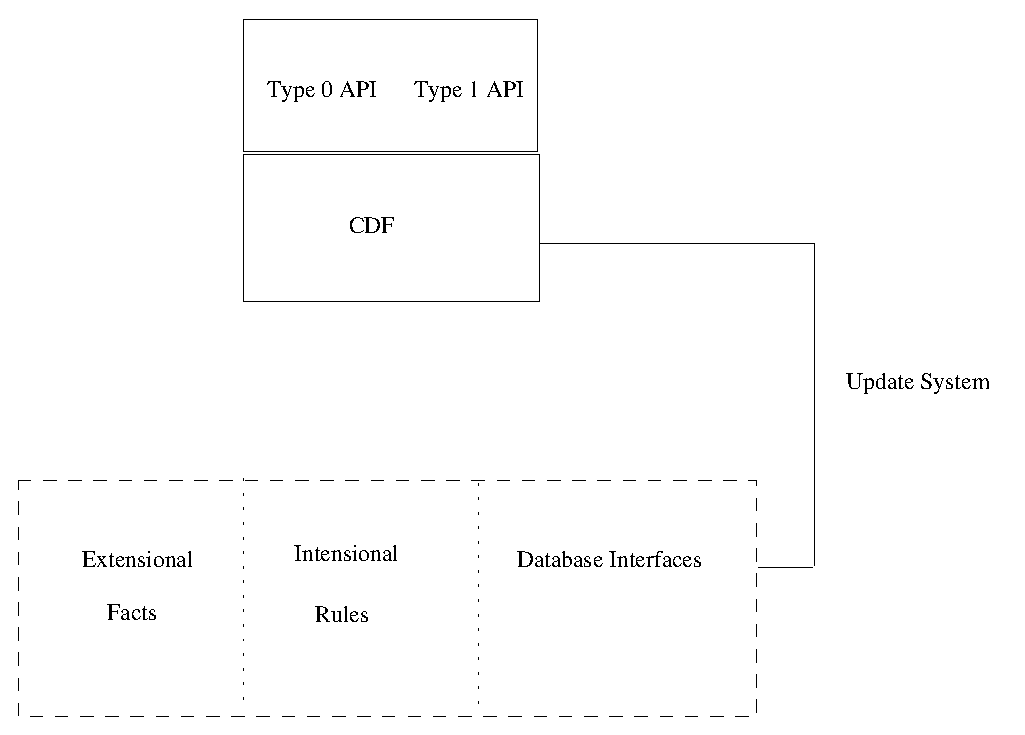
\epsfig{file=Figures/arch.eps,width=0.80\textwidth}}
%\caption{A High-Level Architecture of CDF and XJ}
%\label{fig:arch}
%\end{figure}
%--------------

CDF instances can be classified either as Type-0 or a Type-1, each of
which has its own interface.  Type-0 instances are useful for storing
large amounts of information; and consistency and implication in
Type-0 instances is computable in polynomial time.  Type-0 instances
describe classes by existential and universal relations, qualified
number restrictions, and relational hierarchies, but descriptions omit
negation and disjunction. Type-0 instances also support a direct
product construction for objects and classes.  
\comment{
These product classes and objects can be useful for representing
certain types of non-binary relations, and are particularly useful for
incorporating knowledge represented as RDF facts \cite{}.  }
Information in Type-0 CDF instances is tightly coupled to XSB's
query mechanism, and CDF ensures that only the most specific answers
(according to a given inheritance hierarchy) are returned for any
Type-0 query.

Type-1 instances extend Type-0 instances to describe classes using
negation and disjunction, and thus permit descriptions that are
equivalent to an expressive description logic.  In fact, a Type-1 CDF
instance can be seen as a knowledge base in which various classes are
described via {\em class expressions}, which correspond to formulas in
description logics.  Reasoning in Type-1 instances is done via the CDF
theorem-prover.  Using the Type-1 API, users may ask whether a given
class or object is consistent, whether a given class expression is
consistent with a class or object; or whether a given class expression
is entailed by a given class or object.  The problems of determining
consistency or entailment of a Type-1 class expression have a high
degree of complexity.  To solve these problems the CDF theorem prover
uses several heuristics, but a determined (or unlucky) user can always
find class expressions that requires a lot of time to check.

Of course, ontology management systems require many features in
addition to reasoning and representation features \cite{MGPS03}.  We
mention some of these features.

\begin{itemize}
\item {\em A Semantic Checking System}.  CDF has various mechanisms for
ensuring consistency of objects and classes both at the Type-0 or
Type-1 level.  Various levels of consistency can be checked during
various operations on the CDF instance.
%
\item {\em A Component System}. Reusability of ontologies is supported
by the {\em component} structure of CDF.  An ontology component may be
maintained by separate users or organizations in different locations
and assembled in various ways by applications.
%
\item {\em A Concurrency System}. (Not open-source) Based on the
component structure, the {\em concurrency} mechanism for CDF allows
users to update their own CDF instances and to periodically update a
common store. Naturally, the various mechanisms in CDF for ensuring
consistency that are vital to ensuring coherency when users update
their systems concurrently.
%
\item {\em Database Interfaces}. (Non open-souce) CDF supports various
interfaces to databases so that CDF facts can be stored in a database
or mapped to database tables.
\end{itemize}

Based on these features, CDF can support user interfaces in a number
of ways.  One of the most convenient is to use a XSB/Java interface
such as InterProlog~\cite{Cale01} or JAXSB~(see
\texttt{http://xsb.sourceforge.net}) and then write a user interface in
Swing or some other Java Graphics library.  One of the easiest ways to
do this is to make use of the {\em XJ system} which allows Swing Gui
objects to be represented as Prolog terms (the XJ system is non
open-source) From a systems perspective, a graphical interface is then
written XJ library Swing widgets or specialized XJ-CDF Swing widgets.
CDF per-se has the following graphical packages and applications.
%
\begin{itemize}
%
\item {\em An XJ Caching System}. Adds and deletes to CDF are extended
with a notification mechanism so that Java Swing objects (created with
XJ, XSB's graphics system) reflect the state of CDF even when it
dynamically changes.
%
\item {\em A Visual Editor}. Finally,  CDF supports a graphical editor
that allows users both to visualize an ontology and to perform the
functions mentioned so far.
\end{itemize}
%
Extensional facts, intensional rules, updates, the Type-0 and Type-1
interfaces, consistency checking predicates and the full component
system are available as an open-source package for XSB.  Other
features, concurrency mechanisms, specialized database interfaces, XJ
support and the editor are not yet open-source, but are included in
this manual to indicate the types of applications that can be
constructed with CDF.

%-----------------------------------------------------------
\section{The Meaning of Type-0 CDF Instances} \label{sec:type0} 

Facts in both Type-0 and Type-1 CDF instances are closely related to
class expressions in description logics.  However, because CDF often
stores class expressions as Prolog facts in an unconventional way, and
because description logics may not be familiar to a logic programming
audience, we present here a somewhat formal introduction to how CDF
represents knowledge.  Users without a mathematical background can
ignore the various axioms and formal definitions that are presented in
this chapter.  Our approach is to introduce a semantics of CDF based
on a translation of a {\em CDF instance} into a set of first-order
logic sentences that constitute an {\em Ontology Theory} whose models
are the models of a CDF instance.  For simplicity of presentation the
description of CDF instances in this section omits certain details
about components, extensional facts and intenstional rules, and other
topics that will be introduced in later chapters.

We illustrate aspects of CDF by means of an example drawn from
electronic commerce.  Health care organizations, such as hospitals,
clinics, etc., sometimes have difficulties in buying disposable
medical devices such as sutures, bandages, gloves, and so on.  These
difficulties arise from the fact that these devices may be quite
specialized: for instance some sutures are used only for particular
type of surgery on a particular organ.  At the same time, since these
devices are disposable, they may need to be purchased frequently.  We
consider concretely the class of {\em absorbable sutures}, which are
used for stitching and securing tissues, and which can be absorbed by
the human body.  Information below is adapted from he U.S. Defence
Logistics Information Service \url{http://www.dlis.mil}, from the
Universal Standard Products and Services Classification~\cite{UNSPSC},
as well as from websites of various commercial medical supply
companies.

\subsection{Type-0 CDF Instances} \label{sec:type0} 

We begin with the syntax of Type-0 instances~\footnote{The syntax for
  identfiers is simplified here, and differs in the actual CDF
  implementation. See Section~\ref{sec:instance}.}:

\begin{definition}[Type-0 Instances: Semantic Level] \label{def:ids}
A {\em Type-0 CDF instance} is a finite set of ground facts for the
predicates \pred{isa/2}, \pred{hasAttr/3}, \pred{allAttr/3},
\pred{classHasAttr/3}, \pred{minAttr/4}, and \pred{maxAttr/4}.  An {\em
identifier} is either a constant or a term.  The arguments of these
predicates are {\em concrete identifiers}, where a term $T$ is an
identifier iff $T$ has the functor symbol {\tt cid/1}, {\tt oid/1},
{\tt rid/1}, or {\tt crid/1} whose argument is either

\begin{enumerate}
\item a constant; or 
\item a term $f(I_1,\ldots,I_n)$ where $I_1,\ldots,I_n$ are identifiers.
\end{enumerate}
In the first case, an identifier is called {\em atomic}; in the second
it is called a {\em product identifier}.
\end{definition}

Despite the simple syntax of Type-0 CDF instances, their semantics
differs from the usual semantics assigned to facts in Prolog.
Identifiers identify sets of objects, or binary relations between
objects.  Furthermore, the facts of a Type-0 CDF instance can
implicitly denote inheritance of various relationships among classes
and objects, as well as inheritance constraints about what
relationships are allowed.

\subsection{Simple Taxonomies in CDF}

\begin{example} \rm \label{ex:suture1}
The following CDF instance illustrates a fragment of a taxonomy for
medical equipment.
%-------------------------------------------
{\tt  {\small 
\begin{tabbing}
foo\=foo\=foo\=foo\=foo\=foo\=foooo\=foooooooooooooooo\=\kill
isa(cid(medicalEquipment),cid('CDF Classes'))  \\
\> isa(cid(woundCareProducts),cid(medicalEquipment)) \\
\> \> \>  isa(cid(suturesAndRelatedProducts),cid(woundCareProducts)) \\
\> \> \> isa(cid(sutures),cid(suturesAndRelatedProducts))  \\
\> \> \> \> isa(cid(absorbableSutures),cid(sutures))  \\
\> \> \> \> isa(cid(nonAbsorbableSutures),cid(sutures)) \\
\> \\
\> \> \>   isa(oid(sutureU245H),cid(absorbableSutures))  \\
\> \> \> \> \>   isa(oid(suture547466),cid(sutures)) 
\end{tabbing} }} 
%-------------------------------------------
\noindent
In CDF, sets of objects are termed {\em classes} to stress the
informality of its sets from the perspective of set theory, and class
identifiers have the functor {\tt cid/1}.  One can read the fact
\begin{verbatim}
      isa(cid(nonAbsorbableSutures),cid(sutures))
\end{verbatim}
as ``all elements in the class {\tt cid(nonAbsorbableSutures)} are
also in the class {\tt cid(sutures)}'' --- in other words, that {\tt
cid(nonAbsorbableSutures)} is a subclass of {\tt cid(sutures)}.
Object identifiers have the functor {\tt oid/1}, and denote classes
with cardinality 1, or {\em singleton classes}.  The fact
\begin{verbatim}
      isa(oid(sutureU245H),cid(absorbableSutures))
\end{verbatim}
can be read as ``the element of the singleton class {\tt
oid(sutureU245H)} is in the class {\tt cid(absorbableSutures)}''.
Note that {\tt cid(absorbableSutures)} is (potentially) more specific
than the class {\tt cid(sutures)}, to which {\tt oid(suture547466)}
belongs.  The class {\tt cid('CDF Classes')} is taken to contain all
objects in the domain of discourse.  All identifiers in this simple
taxonomy are atomic.

The decision of whether to denote an entity as an object or as a class
depends on the use of a given CDF instance.  Here, a given part number
can specify a number of physical parts, but the physical parts are
taken to be identical for the purposes of this instance.  However, if
we were constructing a CDF instance for warehouse management, the
above objects might be better represented as classes, and the physical
objects represented as CDF objects.
\end{example} 

Implicit in the above example is the fact that we use the term {\em
object identifiers} or {\em objects} to denote singleton classes,
class identifiers to denote all classes (including singleton classes).
Elements cannot be denoted directly by CDF facts, but only through
singleton classes that contain them (and are isomorphic to them).  At
this point, we can begin defining the semantics of Type-0 CDF
instances.

%-------------------
\begin{definition} \label{def:ontolang}
\index{ontology language} \index{ontology structure} \index{ontology
theory}
%
An {\em ontology language} is a first-order language with equality
containing the predicates: {\em isClass/1, isElt/1, isRel/1, isCrel/1,
elt/2, rel/3, and crel/3}, and a countable set of constants.  An {\em
ontology structure} is a structure defined over an ontology language.
An {\em ontology theory} is a set of first-order sentences formed over
an ontology language that includes a set of {\em core axioms}, defined
below, along with the defined predicate:
\[
isObj(X) =_{def} isClass(X) \wedge 
	((elt(E_1,X) \wedge elt(E_2,X)) \Rightarrow E_1 = E_2)
\]
If $\cT$ is an ontology theory formed over an ontology
language $\cL$, an ontology structure $S$ over $\cL$ is a model of
$\cT$ if every sentence of $\cT$ is satisfied in $S$.
\end{definition}
%-------------------

\index{sorting predicates}
By convention we assume that the variables in an ontology language are
indexed by the set of natural numbers.  In this paper we will restrict
our attention to ontology languages whose constant and function
symbols are identifiers as described in Definition~\ref{def:ids}.
Informally $isClass/1$ indicates that an identifier $I$ is a class
name or {\em class identifier}; $isElt/1$ indicates that an identifier
$I$ is an element of a class; $isRel/1$ that $I$ is a {\em relation
identifier}; and $isCrel/1$ that $I$ is a {\em class-relation
identifier}; and $isObj/1$ that $I$ is an {\em object identifier}.  We
sometimes call these 5 predicates {\em sorting predicates}.
$elt(E,C)$ indicates that an element $O$ is a member of class
identifier $C$; $rel(O_1,R,O_2)$ indicates that an element $E_1$ has a
$R$ relation to an element $E_2$; and $crel(C_1,R,E)$ indicates that
the class identifier $C_1$ has a $R$ relation to an object identifier
$E$.

The first core axiom ensures that objects, classes, relations and
class-relations all have distinct identifiers within an ontology
language.
%-----------
\begin{axiom}[Distinct Identifiers] \label{ax:distinct}
\index{axioms!distinct identifiers} 
\ \\
\begin{tabbing}
foo\=foo\=foo\=foo\=foo\=foo\=foooo\=foooooooooooooooo\=\kill
\> $\neg \exists Id [isClass(Id) \wedge (isElt(Id) \vee isRel(Id) 
	                                 \vee isCrel(Id))] \wedge $ \\
\> $\neg \exists Id [isObj(Id) \wedge (isElt(Id) \vee isCrel(Id))] \wedge $ \\
\> $\neg \exists Id [isElt(Id) \wedge isCrel(Id)] $ 
\end{tabbing}
\end{axiom} 
%-----------

$isClass/1$, $isElt/1$, $isRel/1$, and $isCrel/1$ provide an effective
sorting that extends to all predicates, as the next axiom indicates.

\begin{axiom}[Predicate Sorts] \rm \label{ax:sorts}
\index{axioms!predicate sorts} 
\ \\
\begin{tabbing}
foo\=foo\=foo\=foo\=foo\=foo\=foooo\=foooooooooooooooo\=\kill
\> \> $(\forall X,Y) [elt(X,Y) \Rightarrow (isElt(X) \wedge isClass(Y))]
								\wedge $ \\
\> \> $(\forall X,Y,Z) [rel(X,Y,Z) \Rightarrow (isElt(X) \wedge isRel(Y)
					   \wedge isElt(Z))] \wedge  $ \\
\> \> $(\forall X,Y,Z) [crel(X,Y,Z) \Rightarrow (isClass(X) \wedge isRel(Y)
					   \wedge isElt(Z))] $ \\
\end{tabbing}
\end{axiom} 

%-----------

The following definition of $IdSort$ relates the functors of
identifiers in a Type-0 CDF instance to their sort in an ontology
theory.  It will be used in the various instance axioms to enforce
proper sorting of product identifiers.

\begin{definition}{\bf [IdSort]} \label{def:IdSort}
Let {\em I} is be an identifier. Then {\em IdSort(I)} is equal to {\em
isClass(I)} if the main functor symbol of {\em I} is {\tt cid/1}; {\em
isObj(I)} if the main functor symbol of {\em I} is {\tt oid/1}; {\em
isRel(I)} if the main functor symbol of {\em I} is {\tt rid/1}; and
{\em isCrel(I)} if the main functor symbol of {\em I} is {\tt crid/1}.
\end{definition}

%-----------------------------------------------------------------------------------------
\comment{
\begin{definition}{\bf [IdSort]}  Let {\em I} is be an identifier, and
$\cI$ be the set of identifiers occurring in {\em I}. Then
%
\[ IdSort(I) =_{def} \bigwedge_{I' \in \cI} Sort(I') \]
%
where {\em Sort(I)} is equal to {\em isClass(I)} if the main functor
symbol of {\em I} is {\tt cid/1}; {\em isObj(I)} if the main functor
symbol of {\em I} is {\tt oid/1}; {\em isRel(I)} if the main functor
symbol of {\em I} is {\tt rid/1}; and {\em isCrel(I)} if the main
functor symbol of {\em I} is {\tt crid/1}.
\end{definition}
}
%-----------------------------------------------------------------------------------------

From Definitions~\ref{def:IdSort} and~\ref{def:ontolang}, it is easy
to see that for any object identifier $O$, $IdSort(O) = isObj(O)$, and
$isObj(O) \Rightarrow isClass(O)$.

%-----------
\begin{instance} [Translation of {\tt isa/2}] \rm 
For each fact of the form {\tt isa(Id$_1$,Id$_2$)} add the axiom
\ \\
\begin{tabbing}
foo\=foo\=foo\=foo\=foo\=foo\=foooo\=foooooooooooooooo\=\kill
\> $ IdSort(Id_1) \wedge IdSort(Id_2) \wedge $ \\

\> \> $ (((isClass(Id_1) \wedge isClass(Id_2)) \wedge
	(\forall X) [elt(X,Id_1) \Rightarrow elt(X,Id_2)]) \vee $ \\

%\> \> $ ((isObj(Id_1) \wedge isClass(Id_2)) \wedge elt(Id_1,Id_2)) \vee $ \\

\> \> $ ((isRel(Id_1) \wedge isRel(Id_2)) \wedge
	(\forall X,Y)[rel(X,Id_1,Y) \Rightarrow rel(X,Id_2,Y)]) \vee $ \\

\> \> $ ((isCrel(Id_1) \wedge isCrel(Id_2)) \wedge
	(\forall X,Y)[crel(X,Id_1,Y) \Rightarrow crel(X,Id_2,Y)])) $ 
\end{tabbing}
denoted as {\tt isa(Id$_1$,Id$_2$)}$^{\cI}$.
\end{instance}
%-----------

Note that the reflexive and transitive closure of {\tt isa/2} is an
immediate consequence of its translation rule.  The next axiom is
technical.  It is important for the semantics of relations that each
class have at least one member.
%-----------
\begin{axiom}[Non-Empty Classes] \label{ax:nonnull}
\index{axioms!non-empty classes} 
\[ (\forall X) [isClass(X) \Rightarrow (\exists Y) [elt(Y,X)]] \]
\end{axiom} 
%-----------

The last core axiom for these predicates ensures is that each class is
a subclass of {\tt cid('CDF Classes')}.

%-----------
\begin{axiom}[Domain Containment] \label{ax:contained}
\index{axioms!domain containment} 
\[ (\forall X) [isElt(X) \Rightarrow elt(X,cid('CDF\ Classes'))] \]
\end{axiom} 
%-----------

\subsection{General Relations between Objects in  Classes}

\begin{example} \rm \label{ex:suture2}
The class {\tt cid(sutures)} can be further defined by its relations
to other classes.  For instance, an object in {\tt cid(sutures)} may
have a designation of its needle design indicating whether it is to be
used for abdominal surgeries, thoracic surgeries, or other purposes.
This information is indicated by the following CDF facts:
%
{\small
\begin{tabbing}
fooo\=foo\=foo\=foo\=fooooooooooooooooooooooooooooooo\=ooooooooooooo\=\kill
\> {\tt isa(rid(hasNeedleDesign),rid('CDF Relations'))} \\
\\
\> {\tt isa(cid(domainTypes),cid('CDF Classes'))} \\
\> \> {\tt isa(cid(needleDesignTypes),cid(domainTypes))} \\
\> \> \> {\tt isa(cid(Abdominal),cid(needleDesign))} \\
\> \> \> {\tt isa(cid(Abscisson),cid(needleDesign))} \\
\> \> \> {\tt isa(cid('Adson Dura'),cid(needleDesign))} \\
\> {\it \% 126 other values..}  \\
\\
\> {\tt allAttr(cid(sutures),rid(hasNeedleDesign),cid(needleDesign))} 
\end{tabbing}
}
%
\noindent
The {\tt allAttr/3} fact above can be read as ``if any object in {\tt
cid(absorbableSutures)} has a {\tt rid(hasNeedleDesign)} relation, it
must be to an object in the class {\tt cid(needleDesign)}''.  That
{\tt hasNeedleDesign} is a relation is indicated by clothing it in the
functor {\tt rid/1}.  This relation is an immediate subclass of all
{\tt CDF Relations} which in turn is taken to represent the universal
binary relation over the domain of discourse.  Thus the {\tt
allAttr/3} fact effectively types the range of {\tt
rid(hasNeedleDesign)} relations, stemming from objects in the class
{\tt cid(absorbableSutures)}, but it does not indicate the existence
of such a relationship.  From a user's point of view, the {\tt
rid(hasNeedleDesign)} relation can be thought of as an optional
attribute for a given {\tt cid(absorbableSutures)} object.  Sample
values for {\tt cid(hasNeedleDesignTypes)} are also given.
\end{example} 

%-------------------

{\tt allAttr/3} provides a simple but powerful mechanism for
inheritance of typing among CDF classes:
%---------------------------------------------------------------------------
\comment{
, as can be seen from the
following translation rule, which uses the defined formula

\[ 
elt(X,Y) =_{def} ((isClass(Y) \wedge elt(X,Y)) \vee (isObj(Y) 
			\wedge X = Y))
\] }
%---------------------------------------------------------------------------

\begin{instance} [Translation of {\tt allAttr/3}] \rm 
For each fact of the form {\tt allAttr(Id$_1$,Rid,Id$_2$)} add the instance
axiom: 
\begin{tabbing}
foo\=foo\=foo\=foo\=foo\=foo\=foooo\=foooooooooooooooo\=\kill
\> $ IdSort(Id_1) \wedge IdSort(Rid) \wedge IdSort(Id_2) \wedge $ \\
\> \> $ IsClass(Id_1) \wedge IsRel(Rid) \wedge IsClass(Id_2) \wedge $ \\
\> \> $(\forall X, Y) [(elt(X,Id_1) \wedge rel(X,Rid,Y))
					\Rightarrow elt(Y,Id_2)] $
\end{tabbing}
denoted as {\tt allAttr(Id$_1$,Rid,Id$_2$)$^{\cI}$}.
\end{instance}

%----------------------
\comment{
\begin{tabbing}
foo\=foo\=foo\=foo\=foo\=foo\=foooo\=foooooooooooooooo\=\kill
\> $ IdSort(Id_1) \wedge IdSort(Rid) \wedge IdSort(Id_2) \wedge $ \\
\> \> $ (IsClass(Id_1) \vee isObj(Id_1)) \wedge IsRel(Rid) \wedge 
	 (IsClass(Id_2) \vee isObj(Id_2)) \wedge $ \\
\> \> $(\forall X, Y) [(elt(X,Id_1) \wedge rel(X,Rid,Y))
					\Rightarrow elt(Y,Id_2)] $
\end{tabbing}
}
%----------------------
\begin{example} \rm \label{ex:hasAttr}
While {\tt allAttr/3} indicates a typing for relations, it does not
indicate that a relation must exist for elements of a class.  This
statement is made by \pred{hasAttr/3}.  The relation {\tt
rid(hasPointStyle)} for the class {\tt cid(absorbableSutures)} is
taken to be required in this schema.  The facts
%
{\small
\begin{tabbing}
fooo\=foo\=foo\=foo\=foooooooooooooooooooooooooooo\=ooooooooooooo\=\kill
\> {\tt allAttr(cid(absorbableSutures),rid(hasPointStyle),cid(pointStyle)) } \\
\> {\tt hasAttr(cid(absorbableSutures),rid(hasPointStyle),cid(pointStyle)) }
\end{tabbing}
}
%
\noindent
indicate not only the range of such relationships, but that such a
relationship must exist.  Indeed, the {\tt hasAttr/3} fact can be read
as ``all objects in the class {\tt cid(absorbableSutures)} have a
relation {\tt rid(hasPointStyle)} to an object in the class {\tt
cid(pointStyle)}''.  The facts below also give information about the
{\tt rid(hasPointStyle)} relation.
%
{\small
\begin{tabbing}
fooo\=foo\=foo\=foo\=foooooooooooboooooooooooooooo\=ooooooooooooo\=\kill
\> {\tt isa(cid(pointStyle),cid(domainTypes))} \\
\> {\tt isa(cid(regularCuttingEdge),cid(pointStyle))} \\
\> {\tt isa(cid(reverseCuttingEdge),cid(pointStyle))} \\
\> {\tt isa(cid(scalpelPoint),cid(pointStyle))} \\
\> {\it \% 10 other values.} \\
\\
\> {\tt hasAttr(oid(sutureU245H),rid(hasPointStyle),cid(regularCuttingEdge))}
\end{tabbing}
} 
\noindent
The last of the above facts can be read as ``the object {\tt
oid(sutureU245H)} has a {\tt rid(hasPointStyle)} relation to an object
in the class {\tt cid(pointStyle)}''.  
\end{example}

Not surprisingly, the definition of {\tt hasAttr/3} bears some
similarity to that of {\tt allAttr/3}.

\begin{instance} [Translation of \pred{hasAttr/3}] \rm 
For each fact of the form {\tt hasAttr(Id$_1$,Rid,Id$_2$)} add the instance
axiom: 
\begin{tabbing}
foo\=foo\=foo\=foo\=foo\=foo\=foooo\=foooooooooooooooo\=\kill
\> $ IdSort(Id_1) \wedge IdSort(Id_2) \wedge IdSort(Id_2) \wedge $ \\
\> \> $ IsClass(Id_1) \wedge IsRel(Rid) \wedge
	 IsClass(Id_2) \wedge $ \\
\> \> \> $ (\forall X) [elt(X,Id_1) \Rightarrow \exists Y [rel(X,Rid,Y) 
					\wedge elt(Y,Id_2)]]$
\end{tabbing}
denoted as {\tt hasAttr(Id$_1$,Rid,Id$_2$)$^{\cI}$}.
\end{instance}

We next turn to relational axioms that indicate the cardinality of
various relations.

\begin{example} \rm  \label{ex:maxAttr}
For our purposes, an object in {\tt cid(absorbableSutures)} can be
thought of as consisting of a needle and a thread~\footnote{The thread
is often called a suture.  We are assuming for purposes of
illustration that all sutures are --- in suture-speak --- ``armed''.}.  This is
represented by the facts:
%
{\small
\begin{tabbing}
foo\=foo\=foo\=foo\=foo\=foo\=foooo\=foooooooooooooooo\=\kill
\> {\tt allAttr(cid(absorbableSutures),rid(hasImmedPart),cid(absSutPart)) } \\
\> {\tt hasAttr(cid(absorbableSutures),rid(hasImmedPart),cid(absSutNeedle)) } \\
\> {\tt hasAttr(cid(absorbableSutures),rid(hasImmedPart),cid(absSutThread)) } \\
\\
\> {\tt isa(cid(absSutPart),cid(suturesAndRelatedProducts))}  \\
\> \> {\tt isa(cid(absSutNeedle),cid(absSutPart)) } \\
\> \> {\tt isa(cid(absSutSuture),cid(absSutPart)) } 
\end{tabbing}
}
%
\noindent
A needle for an absorbable suture is typically made of a different
material than the thread to which the needle is attached.  Each of
these materials may be important in choosing an absorbable suture, and
each of these materials are unique.  The facts
%
{\small
\begin{tabbing}
foo\=foo\=foo\=foo\=foo\=foo\=foooo\=foooooooooooooooo\=\kill
\> {\tt hasAttr(cid(absSutPart),rid(hasMaterial),cid(absSutMaterial)) } \\
\> {\tt maxAttr(cid(absSutPart),rid(hasMaterial),cid(absSutMaterial),1) } \\
\\
\> {\tt isa(cid(material),cid(domainTypes))} \\
\> {\tt isa(cid(absSutMaterial),cid(material)} \\
\> {\tt isa(cid(gut),cid(absSutMaterial))} \\
\> {\tt isa(cid(polyglyconate),cid(absSutMaterial))} \\
\> {\tt isa(cid(polyglyconicAcid),cid(absSutMaterial)) } 
\end{tabbing}
}
%
\noindent
indicate that each {\tt cid(absSutPart)} has a unique material.  The
{\tt maxAttr/4} fact can be read as ``Each object in the class {\tt
cid(absSutPart)} has at most 1 {\tt rid(hasMaterial)} relation to an
object in the class {\tt cid(absSutMaterial)}''.
\end{example}

In order to define the semantics of {\tt maxAttr/4}, let
$\exists^{\leq n}X_m[ \phi(X,Z)]$ be defined as an abbreviation for
the formula
\[
  \exists x_m,...,\exists x_{m+n} [\bigwedge_{m \leq i \leq m+n} 
	\phi(x_i,\overline{z}) 
	\Rightarrow \bigvee_{m \leq i < j \leq m+n} x_i  = x_j]
\]
i.e., for the formula indicating that there are at most $N$ non-equal
elements satisfying $\phi(x,z)$.  The abbreviation $\exists^{\geq N}$
is defined similarly to indicate that a formula is satisfied by at
least $N$ non-equal elements.

\begin{instance} [Translation of {\tt maxAttr/4}] \rm 
For each fact of the form {\tt maxAttr(Id$_1$,Rid,Id$_2$,N)} add the instance
axiom: 
\begin{tabbing}
foo\=foo\=foo\=foo\=foo\=foo\=foooo\=foooooooooooooooo\=\kill
\> $ IdSort(Id_1) \wedge IdSort(Id_2) \wedge IdSort(Id_2) \wedge $ \\
\> \> $ IsClass(Id_1) \wedge IsRel(Rid) \wedge
	 (IsClass(Id_2) \wedge $ \\
\> \> \> $ (\forall X) [elt(X,Id_1) \Rightarrow \exists^{\leq N} Y [rel(X,Rid,Y) 
					\wedge elt(Y,Id_2)]]$
\end{tabbing}
denoted as {\tt maxAttr(Id$_1$,Rid,Id$_2$,N)$^{\cI}$}.
\end{instance}

A corresponding predicate, {\tt minAttr/4} is used to indicate a
minimality restriction on a relation.  {\tt minAttr/4} is defined
similarly to {\tt maxAttr/4}, but using $\exists^{\geq N}$ rather than
$\exists^{\leq N}$.  Indeed, the predicate
%
{\small {\tt 
\begin{tabbing}
foo\=foo\=foo\=foo\=foo\=foo\=foooo\=foooooooooooooooo\=\kill
\> hasAttr(cid(absSutPart),rid(hasMaterial),cid(absSutMaterial)).
\end{tabbing}
} }
%
\noindent
could be replaced by the predicate
%
{\small {\tt 
\begin{tabbing}
foo\=foo\=foo\=foo\=foo\=foo\=foooo\=foooooooooooooooo\=\kill
\> minAttr(cid(absSutPart),rid(hasMaterial),cid(absSutMaterial),1).
\end{tabbing}
} }
%
\subsection{Class Relations}
Each of the predicates discussed so far are inheritable in their first
argument.  For instance, the fact
{\small {\tt 
\begin{tabbing}
foo\=foo\=foo\=foo\=foo\=foo\=foooo\=foooooooooooooooo\=\kill
\> hasAttr(cid(absSutPart),rid(hasMaterial),cid(absSutMaterial)).
\end{tabbing}
} } 
%
\noindent
implies that every subclass of {\tt cid(absSutures)} will have a
material in the class {\tt cid(absSutMaterial)}.  However, classes may
have relations that do {\em not} hold for their subclasses or members.
For instance, a finite set may have a given cardinality, but its
proper subsets will have a different cardinality.  Such relations are
termed {\em class relations}.

%-------------------
\begin{example} \label{ex:strel} \rm 
A practical example of a class relation comes from an application that
may be called part equivalency matching.  In this application, the
possible attributes for a class of parts are given various weights.
Two parts match if the sum of the weights of their attributes that
match are above a given threshold.  The weighting for the {\tt
cid(pointStyle)} of sutures might be given as:
%----------------------------------
{\small 
{\tt 
\begin{tabbing}
foo\=foo\=foo\=foo\=foo\=foo\=foooo\=foooooooooooooooo\=\kill
\> isa(cid(pointStyleWeight),cid('CDF Classes')) \\
\> \> isa(cid(highWeight),cid(pointStyleWeight)) \\
\> \> isa(cid(lowWeight),cid(pointStyleWeight)) \\
\\
\> classHasAttr(cid(sutures),crid(pointStyleWeight),cid(highWeight))
\end{tabbing}
} }
%----------------------------------
\noindent
The {\tt classHasAttr/3} fact can be read as ``the class {\tt
cid(sutures)} has a {\tt crid(pointStyleWeight)} relation to an object
in {\tt cid(highWeight)}.  Matching weights are made non-inheritable
via {\tt classHasAttr/3} because a weight may depend on a given
classification of a part.  For instance if a part were classified as a
{\tt cid(nonAbsorbableSuture)}, its {\tt cid(pointStyle)} might weigh
less (or more) for determining whether two sutures are equivalent.
\end{example}
%------------------
\begin{instance} [Translation of {\tt classHasAttr/3}] \rm 
For each fact of the form {\tt classHasAttr(Id$_1$,CRid,Id$_2$)} add the
instance axiom: 
\begin{tabbing}
foo\=foo\=foo\=foo\=foo\=foo\=foooo\=foooooooooooooooo\=\kill
\> $ IdSort(Id_1) \wedge IdSort(CRid) \wedge IdSort(Id_2) \wedge $ \\
\> \> $ IsClass(Id_1) \wedge IsCrel(CRid) \wedge isClass(Id_2) \wedge $ \\
\> \> \> $ (\exists X) [elt(X,Id_2) \wedge crel(Id_1,CRid,X)] $
\end{tabbing}
denoted as {\tt classHasAttr(Id$_1$,Rid,Id$_2$)$^{\cI}$}.
\end{instance}
%----------

\subsection{Product Classes}

The above predicates allow the definition of various named binary
relations between classes.  However, binary definitions can sometimes
be inconvenient to use.  For instance, in the part equivalency
matching example, (Example~\ref{ex:strel}), it may be desirable to
make explicit the weight of the match as an indication of the strength
of the match.  The weight could be made explicit by a series of
definitions
%-------------------------------------------
{\small 
{\tt 
\begin{tabbing}
foo\=foo\=foo\=foo\=foo\=foo\=foooo\=fooooooooooooooo\=\kill
\> allAttr(\cid{dlaPart},\rid{suturesRusMatch\_low},\cid{suturesRusPart}) \\
\> : \\
\> allAttr(\cid{dlaPart},\rid{suturesRusMatch\_high},\cid{suturesRusPart})
\end{tabbing}
} } 
%----------------------------------
\noindent
indicting that a given part has a match of weight {\em low} through
{\em high}.  However, for a scale with a large number of values,
defining matches in this way is time-consuming and prone to errors.
To address this, we first define a new class {\tt \cid{matchScale}}
containing as subclasses the various match levels.  We then combine
{\tt \cid{matchScale}} with the class {\tt \cid{suturesRusPart}} in a
product with a {\em product identifier}, as in the following fact
%-------------------------------------------
{\small 
{\tt 
\begin{tabbing}
foo\=foo\=foo\=foo\=foo\=foo\=foooo\=foooooooooooooooo\=\kill
 
allAttr(\cid{dlaPart},\rid{suturesRusMatch}, \\
\> \> \> \> \cid{partMach(\cid{suturesRusPart},\cid{matchScale})})
\end{tabbing}  } }
\noindent 
which indicates that a {\tt \cid{dlaPart}} can have a {\tt
\cid{suturesRusMatch}} to an object in the {\tt partMatch/2}  class,
which has both a {\tt \cid{suturesRusPart}} component and a {\tt
\cid{matchScale}} component.

%-------------------------------------------------------------------

We capture the intuition behind product classes through the following
axiom schemas.  The first indicates that product identifiers 
are constructed from {\em constituent identifiers} of the same sort.

\begin{axiom}[Downward Closure] \label{ax:downcl}
\index{axioms!downward closure}
\ \\
For each product identifier $\cid{f(x_1,\ldots,x_n)}$,
$\oid{f((x_1,\ldots,x_n)}$, $\rid{f(x_1,\ldots,x_n)}$, and
$c\rid{f((x_1,\ldots,x_n)}$ the following axiom is added,
\begin{tabbing}
foo\=foo\=foo\=foo\=foo\=foo\=foooo\=foooooooooooooooo\=\kill
\> $isClass(\cid{f(x_1,\ldots,x_n)}) \Rightarrow 
	isClass(x_1) \wedge \ldots \wedge isClass(x_n) $\\
\> $isObj(\oid{f(x_1,\ldots,x_n)}) \Rightarrow 
	isObj(x_1) \wedge \ldots \wedge isObj(x_n) $\\
\> $isRel(\rid{f(x_1,\ldots,x_n)}) \Rightarrow 
	isRel(x_1) \wedge \ldots \wedge isRel(x_n) $\\
\> $isCrel(\crid{f(x_1,\ldots,x_n)}) \Rightarrow 
	isCrel(x_1) \wedge \ldots \wedge isCrel(x_n) $
\end{tabbing}
\end{axiom}

With this axiom, along with the use of $IdType/1$ in the various
instance axioms, we will sometimes refer to a CDF identifier $I$ as a
class identifier if its outer functor is {\tt cid/1}, an object
identifier if its outer functor is {\tt oid/1} etc.  The next axiom
associates product classes with the objects they contain.

\begin{axiom}[Implicit Subclassing] \label{ax:implsc}
\index{axioms!implicit subclassing} 

\begin{enumerate}
\item For each product identifier $cid(f(x_1,\ldots,x_n))$ or 
$oid(f(x_1,...,x_n))$, the following axioms are added for $x_i, 1 \leq i
\leq n$:
\[
(\forall E) [(elt(E,y_i) \Ra elt(E,x_i)) \Ra \\
	(\forall E') [elt(E',f(x_1,...x_n))[x_i/y_i] \Rightarrow elt(E',f(x_1,...x_n))]]
\]

\item For each product identifier $rid(f(x_1,\ldots,x_n))$ the
following axioms are added for $x_i, 1 \leq i 
\leq n$:
\begin{tabbing}
foo\=foo\=foo\=foo\=foo\=foo\=foooo\=foooooooooooooooo\=\kill
\> $(\forall E_1,E_2) [(rel(E_1,y_i,E_2) \Ra rel(E_1,x_i,E_2)) \Ra$ \\
\> \> $(\forall E'_1,E'_2) [rel(E'_1,f(x_1,...x_n),E'_2)[x_i/y_i] \Ra rel(E'_1,f(x_1,...x_n),E'_2)]]$
\end{tabbing}
\end{enumerate}
\end{axiom}

%-------------------------------------------
\comment{
\begin{axiom}[Implicit Subclassing] \label{ax:implsc}
\begin{enumerate}
\item For each product identifier $\oid{f(x_1,\ldots,x_n)}$ the
following axiom is added:  
\[(\forall O) [elt(O,\cid{f(x_1,\ldots,x_n)})
	\Ra (O = \oid{f(y_1,\ldots,y_n)} \wedge 
  		  elt(y_1,x_1) \wedge \ldots \wedge elt(y_n,x_n))] \]

\item For each product identifier $\cid{f(x_1,\ldots,x_n)}$ and for
each atomic identifier $\cid{c}$ the following axiom is
added:
\[ (\forall C) 
   ([elt(\oid{f(x_1,\ldots,x_n)},C)] \Ra (C = \cid{f(y_1,\ldots,y_n)}
   \vee C = \cid{c})) \]
\end{enumerate}
\end{axiom}
}
%-------------------------------------------

\begin{example} \rm
Axiom~\ref{ax:downcl} simply states that identifier types cannot be
mixed within a product identifier.  For instance, if {\tt
\oid{matchLevelN}} is an object in the {\tt \cid{matchScale}},
then the identifier 

{\tt \cid{partMatch(\cid{suturesRusMatch},\oid{matchLevelN})}}

\noindent
is improperly formed.  On the other hand, if {\tt \oid{sutureU245H}} is in
the class {\tt \cid{suturesRusPart}}, then the identifier {\tt
\oid{partMatch(\oid{sutureU245H},\oid{matchLevelN})}} is a product
identifier that is also an object identifier.

Axiom~\ref{ax:implsc} also means that the inheritance relation of a
product class is partly determined by the inheritance relation of its
constituent elements.
\end{example}

\comment{
Core Axiom~\ref{ax:implsc} can be used either to set up equality
constraints on a model of a CDF instance, or it can be used to
determine which CDF instances have free models (as explained in the
next section).  The following example illustrates the first use.

\begin{example} \rm \label{ex:equality}
Suppose we have the CDF instance
{\small 
{\tt 
\begin{tabbing}
foo\=foo\=foo\=foo\=foo\=foo\=foooo\=foooooooooooooooo\=\kill
\> isa(\cid{a},\cid{f(a)}.
\end{tabbing} } } 
\noindent
By Core Axiom~\ref{ax:nonnull} (Non-empty Classes), {\tt \cid{a}} has
at least one element, which can be called {\tt \oid{a1}}.  By the
instance axiom for the above fact, {\em elt(\oid{a1},\cid{f(a)}}.  By
Core Axiom~\ref{ax:implsc}(1), it must be the case that 
%
\[ \oid{a1} = \oid{f(Y)} \wedge elt(Y,\cid{a}) \]
%
If we take $Y = \oid{a1}$, then this means that 
%
$ \oid{a1} = \oid{f(\oid{a1})} $
% 
so that the above fragment has a model $\cM$ with a single individual
(in the universe of $\cM$) to which all object identifiers are mapped,
and that has a $elt/2$ relation to each individual to which a class
identifier is mapped (among other models).
\end{example}
}

%\input{models}

\section{Implementation and System Features} \label{sec:impl}
%
In this section we describe how the CDF system implements the
semantincs of Section~\ref{sec:type0} , as well as many other features
for ontology management.  We begin by describing CDF identifiers,
facts, and rules in Section~\ref{sec:instance}.  The Type-0 query
interface, based on tabled resolution is described in
Section~\ref{sec:type0query}.  Section~\ref{sec:type0query} describes
the Type-1 API, which is based on the CDF therorem prover.  Update and
consistency predicates for CDF are described in
Section~\ref{sec:update}.  Section~\ref{sec:config} describes how to
configure CDF, along with predicates that allow the user to examine
aspects of the CDF state.  Section~\ref{sec:components} describes
basic I/O for CDF, along with a more sophisticated {\em component}
system that is built on top of basic I/O.  Section~\ref{sec:database}
describes database interfaces for CDF, and
Section~\ref{sec:concurrency} describes concurrency support.

%----------------------------------------------------


\subsection{CDF Instances} \label{sec:instance}

Part~\ref{part:semantics} simplified the syntax of CDF instances in
certain ways.  In this section we describe those aspects of the actual
CDF implementation that differ from the abstract presentation
Part~\ref{part:semantics}.

The first major difference concerns CDF identifiers.

\index{CDF Identifer}
\index{component tag}
\begin{definition}[CDF Identifiers] \label{def:cdfids}
A {\em CDF identifier} has the functor symbol {\tt cid/2}, {\tt
oid/2}, {\tt rid/2}, or {\tt crid/2}.  The second argument of a CDF
identifier is a Prolog atom and is called its {\em component tag},
while the first argument is either
\begin{enumerate}
\item a Prolog atom or 
\item a term $f(I_1,\ldots,I_n)$ where $I_1,\ldots,I_n$ are CDF identifiers.
\end{enumerate}
In the first case, an identifier is called {\em atomic}; in the second
it is called a {\em product identifier}.
\end{definition}

Thus in an implementation of, say, Example~\ref{ex:suture1} all
identifiers would have component tags.  For instance the identifier
{\tt cid(absorbableSutures)} might actually have the form {\tt
cid(absorbableSutures,unspsc)} and {\tt oid(sutureU245H)} would have
the form {\tt oid(sutureU245H,sutureRus)}.  These component tags have
two main uses.  First, they allow ontolgies from separate soruces to
be combined, and thus function in a manner somewhat analogous to XML
namespaces.  Second, the component tags are critical to the CDF
component system, described in \secref{sec:components}.

%----------------------------------------------------------------------------
\subsubsection{Extensional Facts and Intensional Rules}

\index{extensional facts} \index{intensional rules}
%
An actual CDF instance is built up of {\em extensional facts} and {\em
intensional rules} defined for the CDF predicates {\tt isa/2} {\tt
allAttr/3}, {\tt hasAttr/3}, {\tt classHasAttr/3}, {\tt coversAttr/3},
{\tt minAttr/4} and {\tt maxAttr/4}.  Extensional facts for these
predicates add the suffix {\tt \_ext} to the suffix name leading to
{\tt isa\_ext/2}, {\tt allAttr\_ext/2} and so on.  Intensional rules
add the suffix {\tt \_int} leading to {\tt isa\_int/2}, {\tt
allAttr\_int/2} etc.

Extensional facts make use of XSB's sophisticated indexing of dynamic
predicates.  Since CDF Extensional Facts use functors such as {\tt
  cid/1} or {\tt oid/1} to type their arguments, traditional Prolog
indexing, which makes use only of the predicate name and outer functor
of the first argument, is unsuitable for large CDF instances.  CDF
extensional facts use XSB's star-indexing (cf. Volume 1 of this
manual).  For ground terms, star-indexing can index on up to the first
five positions of a specified argument.  In addition, various
arguments and combinations of arguments can be used with star-indexing
of dynamic predicates.  The ability to index within a term is critical
for the performance of CDF; also since star-indexing bears
similarities to XSB's trie-indexing~\cite{RRSSW98}, it is spatially
efficient enough for large-scale use.  Section~\ref{sec:config}
provides information on default indexing in CDF and how it may be
reconfigured.

Intensional rules may be defined as XSB rules, and may use any of
XSB's language or library features, including tabling, database, and
internet access.  Intensional rules are called on demand, making them
suitable for implementing functionality from lazy database access
routines to definitions of primitive types.

\begin{example} \rm \label{ex:intrules}
In many ontology management systems, integers, floats, strings and so
on are not stored explicitly as classes, but are maintained as a sort
of {\em primitive type}.  In CDF, primitive types are easily
implemented via intensional rules like the following.
%
{\small {\sf  
\begin{tabbing}
foo\=foo\=foooooooooooooooooooooooooooooooooooooooo\=foo\=\kill
%
\> isa\_int(oid(Float),cid(allFloats)):- \\
\> \> 	(var(Float) -$>$ cdf\_mode\_error ; float(Float). \\
\end{tabbing} } }
\end{example}
%
CDF provides intensional rules defining all Prolog primitive types as
CDF primitive types in the component \component{cdfpt} (see below).
Other, more specialized types can be defined by users by defining
intensional rules along the same lines {\sc fill in 'below'; tabling
and intensional rules}

As mentioned above, the predicate {\tt
immed\_hasAttr/3}, (and {\tt immed\_allAttr/3}, etc) is used to store
basic CDF information that is used by predicates implementing {\tt
hasAttr/3} and other relations.  {\tt immed\_hasAttr/3} itself is
implemented as:
%
{\small {\sf  
\begin{tabbing}
foo\=foo\=foooooooooooooooooooooooooooooooooooooooo\=foo\=\kill
%
\> immed\_hasAttr(X,Y,Z):- hasAttr\_ext(X,Y,Z). \\
\> immed\_hasAttr(X,Y,Z):- hasAttr\_int(X,Y,Z). \\
\> immed\_hasAttr(X,Y,Z):- immed\_minAttr(X,Y,Z,\_). 
\end{tabbing} } }
%
\noindent
The above code fragment illustrates two points.  First, {\tt
immed\_hasAttr/3} is defined in terms of {\tt immed\_minAttr/3},
fulfilling the semantic requirements of Section \ref{sec:type0}.
It also illustrates that {\tt immed\_hasAttr/3} is implemented in
terms both of extensional facts {\tt hasAttr\_ext/3} and intensional
rules {\tt hasAttr\_int(X,Y,Z)}.  

%-------------------------------------------

\subsubsection{The Top-level Hierarchy and Primitive Types}

All CDF instances share the same top-level hierarchy, as depicted in
Figure~\ref{fig:toplevel}.  All classes and objects are subclasses
(through the {\tt isa} relation) to {\tt cid('CDF Classes',cdf)}, all
relations are subrelations of {\tt rid('CDF Object-Object
Relations',cdf)} and all class relations are subrelations of {\tt
crid('CDF Class-Object Relations',cdf)}.
%-------------------------------------------
\index{identifiers!cid('CDF Classes',cdf)}
\index{identifiers!rid('CDF Object-Object Relations,cdf)}
\index{identifiers!crid('CDF Class-Object Relations',cdf)}
\index{identifiers!cid('CDF Primitive Types',cdf)}
\index{identifiers!cid(allIntegers,cdf)}
\index{identifiers!cid(allFloats,cdf)}
\index{identifiers!cid(allAtoms,cdf)}
\index{identifiers!cid(allStructures,cdf)}
\index{identifiers!cid(atomicIntegers,cdf)}

\begin{figure}[htb] 
{\small {\it
\begin{center}
\begin{bundle}{cid('CDF Classes',cdf)}
\chunk{\begin{bundle}{cid('CDF Primitive Types',cdf)}
  \chunk{\begin{bundle}{cid(allIntegers,cdf)\ \ \ \ \ \    }
	\chunk{oid(Integer,cdfpt)}
	\end{bundle} }
  \chunk{\begin{bundle}{cid(allFloats,cdf)\ \ \ \ \ \ }
	\chunk{oid(Float,cdfpt)}
	\end{bundle} }
  \chunk{\begin{bundle}{cid(allAtoms,cdf)\ \ \ \ \ \ }
	\chunk{oid(Atom,cdfpt)}
	\end{bundle} }
  \chunk{\begin{bundle}{cid(allStructures,cdf)\ \ \ \ \ \ }
	\chunk{oid(Structure,cdfpt)}
	\end{bundle} }
  \chunk{\begin{bundle}{cid(atomicIntegers,cdf)}
	\chunk{oid(AInteger,cdfpt)}
	\end{bundle} }
  \end{bundle} } 
\end{bundle}
\end{center}

\ \\
\begin{center}
rid('CDF Object-Object Relations',cdf)
\end{center}

\ \\
\begin{center}
\begin{bundle}{crid('CDF Class-Object Relations',cdf)}
\chunk{crid('Name',cdf)}
\chunk{crid('Description',cdf)}
\end{bundle}
\end{center}
} }
\caption{Built-in Inheritance Structure of CDF}
\label{fig:toplevel}
\end{figure}
%-------------------------------------------

An immediate subclass of {\tt cid('CDF Classes',cdf)} is {\tt cid('CDF
Primitive Types',cdfpt)}.  This class allows users to maintain in CDF
any legally syntactic Prolog element, and forms an exception to
Definition~\ref{def:cdfids}.  Specifically {\tt cid('CDF Primitive
Types',cdf)} contains Prolog atoms, integers, floats, structures and
what are termed ``atomic integers'' --- integers that are represented
in atomic format, e.g. '01234'.  Primitive types are divided into five
subclasses, {\tt cid(allIntegers,cdf)}, {\tt cid(allFloats,cdf)}, {\tt
cid(allAtoms,cdf)}, {\tt cid(allStructures,cdf)}, and {\tt
cid(atomicInteger,cdf)}.  Each of these in turn have various objects
as their immediate subclasses~\footnote{Recall that objects in CDF are
singleton classes.}, whose inheritance relation is defined by an
intensional rule like the one presented in Example~\ref{ex:intrules}.
Thus, if the number 3.2 needs to be added to an ontology, perhaps as
the value of an attribute, it is represented as {\tt oid(3.2,cdfpt)},
and it will fit into the inheritance hierarchy as a subclass of {\tt
cid(allFloats,cdf)}.  The intensional rules are structured so that for
any Prolog syntactic element {\tt X}, when {\tt X} is combined with
the component \component{cdfpt}, then {\tt cid(X,cdfpt)} will be a
subclass of {\tt cid('CDF Primitive Types',cdfpt)}, as will be {\tt
oid(X,cdfpt)}.

\subsubsection{Basic CDF Predicates}

\begin{description}
\ourpredmodrptitem{isa\_ext/2}{usermod}
\ourpredmodrptitem{allAttr\_ext/3}{usermod}
\ourpredmodrptitem{hasAttr\_ext/3}{usermod}
\ourpredmodrptitem{classHasAttr\_ext/3}{usermod}
\ourpredmodrptitem{minAttr\_ext/4}{usermod}
\ourpredmodrptitem{maxAttr\_ext/4)}{usermod}
%\ourpredmodrptitem{coversAttr\_ext/3)}{usermod}
\ourpredmoditem{necessCond\_ext/2)}{usermod}
%
These dynamic predicates are used to store extensional facts in CDF.
They can be called directly from the interpreter or from files that
are not modules, but must be imported from {\tt usermod} by those
files that are modules.  Extensional facts may be added to a CDF system
via \pred{newExtTerm/1} (\secref{sec:update}), or imported from a
\ttindex{cdf\_extensional.P} file (\secref{sec:components}).

\ourpredmodrptitem{isa\_int/2}{usermod}
\ourpredmodrptitem{allAttr\_int/3}{usermod}
\ourpredmodrptitem{hasAttr\_int/3}{usermod}
\ourpredmodrptitem{classHasAttr\_int/3}{usermod}
\ourpredmodrptitem{minAttr\_int/4}{usermod}
\ourpredmodrptitem{maxAttr\_int/4)}{usermod}
%\ourpredmodrptitem{coversAttr\_int/3)}{usermod}
\ourpredmoditem{necessCond\_int/2)}{usermod}
%
These dynamic predicates are used to store intensional rules in CDF.
They can be called directly from the interpreter or from files that
are not modules, but must be imported from {\tt usermod} by those
files that are modules.  Intensional rules may be added to a CDF
system via \pred{???newIntRule/1} (\secref{sec:update}), or imported from
a \ttindex{cdf\_intensional.P} file (\secref{sec:components}).


\ourpredmoditem{immed\_isa/2}{cdf\_init\_cdf}
{\tt immed\_isa(SubCid,SupCid)} is true if there is a corresponding
fact in \pred{isa\_ext/2} or in the intensional rules.  It does not
use the Implicit Subclassing Axiom \ref{ax:implsc}, the Domain
Containment Axiom~\ref{ax:contained}, or reflexive or transitive
closure.

\ourpredmodrptitem{immed\_allAttr/3}{cdf\_init\_cdf}
\ourpredmodrptitem{immed\_hasAttr/3}{cdf\_init\_cdf}
\ourpredmodrptitem{immed\_classHasAttr/3}{cdf\_init\_cdf}
\ourpredmodrptitem{immed\_minAttr/4}{cdf\_init\_cdf}
\ourpredmodrptitem{immed\_maxAttr/4)}{cdf\_init\_cdf}
%\ourpredmodrptitem{immed\_coversAttr/3)}{cdf\_init\_cdf}
\ourpredmoditem{immed\_necessCond/2)}{cdf\_init\_cdf}
Each of these predicates calls the corresponding extensional facts for
the named predicate as well as the intensional rules.  No inheritance
mechanisms are used, and any intensional rules unifying with the call
must support the call's instantiation pattern.


\ourpredmoditem{cdf\_id\_fields/4}{cdf\_init\_cdf}
{\tt cdf\_id\_fields(ID,Functor,NatId,Component)} is true if {\tt ID}
is a legal CDF identifier, {\tt Functor} is its main functor symbol,
{\tt NatId} is its first field and {\tt Component} is its second
field.  This convenience predicate provides a faster way to examine
CDF identifiers than using {\tt functor/3} and {\tt arg/3}.

\end{description}

`\section{The Type-0 Query Interface} \label{sec:type0query}

There are two main design goals behind the Type-0 query interface.
\begin{itemize}
\item to provide a Prolog interface to CDF based on  
the axioms in Chapter~\ref{sec:type0}, and the {\sc inh} proof system
derived from \refsec{sec:inheritance} along with
Proposition~\ref{prop:necesscondinh}.
\item to provide a highly efficient and scalable interface to CDF.
\end{itemize}

Indeed, the Type-0 interface has been used to support CDF instances
containing nearly a million extensional facts that require heavy
manipulation and access, and are used as back-ends to interactive
graphical systems.  As discussed below, this need for efficiency
affects certain aspects of the interface.

\subsection{Virtual Identifiers}
As discussed, Type-0 instances do not make contain facts of the form
\pred{necessCond/2}.  In the implementation of CDF, {\tt necessCond/2}
goals can be called, and their implementation obeys the first-argument
inheritance for {\tt necessCond}.  However, it is important to note
that {\bf the Type-0 interface does not use information in virtual
identifiers} as the following example shows.

\begin{example} \rm 
Consider the CDF instance containing only the fact
{\small 
{\tt 
\begin{tabbing}
foo\=foo\=foo\=foo\=foo\=foo\=foooo\=foooooooooooooooo\=\kill
\> necessCond\_ext(cid(a,test),vid(exists(rid(r,test),cid(b,test)))).
\end{tabbing} } } 
%
\noindent
by the semantics of type 1 ontologies, this CDF instance logically
entails {\small {\tt
\begin{tabbing}
foo\=foo\=foo\=foo\=foo\=foo\=foooo\=foooooooooooooooo\=\kill
\> hasAttr(oid(a,test),rid(r.text),cid(b,text))$^{\cI}$
\end{tabbing} } } 
%
\noindent
However the Type-0 interface will answer ``no'' to the query 
{\small 
{\tt 
\begin{tabbing}
foo\=foo\=foo\=foo\=foo\=foo\=foooo\=foooooooooooooooo\=\kill
\> ?- hasAttr(oid(a,test),rid(r.text),cid(b,text)).
\end{tabbing} } } 
%
\end{example}

\subsection{Computing Irredundant Answers}

Consider the running sutures example of Chapter~\ref{sec:type0} to
which is added a fact
%
{\small 
{\tt 
\begin{tabbing}
foo\=foo\=foo\=foo\=foo\=foo\=foooo\=foooooooooooooooo\=\kill
\> hasAttr(oid(sutureU245H),rid(needleDesign),cid('Adson Dura')).
\end{tabbing} } } 
%
\noindent
Suppose the query {\tt ?-
hasAttr(oid(sutureU245H),rid(needleDesign),Y)} were asked.  Via an
{\sc inh} proof, rhe CDF instance would imply the answers 
%
{\small {\tt
\begin{tabbing}
foo\=foo\=foo\=foo\=foo\=foo\=foooo\=foooooooooooooooo\=\kill
\>  hasAttr(oid(sutureU245H),rid(needleDesign),cid('Adson Dura')) \\
\> hasAttr(oid(sutureU245H),rid(needleDesign),cid(needleDesignTypes)) \\
\>  hasAttr(oid(sutureU245H),rid(needleDesign),cid('CDF Classes))
\end{tabbing} } }
%
\noindent
The last two answers are, of course, redundant according to
Definition~\ref{def:redund}.  Omitting redundant answers is important
both for human comprehension of information in a CDF instance, and to
reduce excessive backtracking in applications.

% TLS coversAttr
Computation of irredundant answers is done in CDF by creating a {\em
preference relation}\ \ on the relations {\tt hasAttr/3}, {\tt
classHasAttr/3}, {\tt allAttr/3}, {\tt minAttr/3}, {\tt maxAttr/3} and
{\tt necessCond} using the techniques of \cite{CuSw02}.  The schematic
code for a query to {\tt hasAttr/3} in which the first argument is
known to be bound, and the second two free, is shown in
Figure~\ref{fig:preference}.  Basic information concerning {\tt
hasAttr/3} within a CDF instance is kept via the predicate {\tt
immed\_hasAttr/3} (and similarly for other CDF relations), and {\tt
hasAttr/3} uses {\tt immed\_hasAttr/3} to compute implications via
inheritance upon demand.  In the compilation of the code in
Figure~\ref{fig:preference}, well-founded negation is used to ensure
that only preferred answers are returned.  It is easy to see by
comparing the preference rules of Figure~\ref{fig:preference} with
Propositions~\ref{prop:inh1}-\ref{prop:inh2}, that the preference rule
ensures that answers are returned only if they are not implied by
other answers.  Similar approaches are used for other query modes and
CDF relations.  

\begin{figure}[htb] 
%-------------------------------------------
{\small {\sf  
\begin{tabbing}
foo\=foo\=foooooooooooooooooooooooooooooooooooooooo\=foo\=\kill
%
\> hasAttr(X,Y,Z):- \\
\> \> 	nonvar(X), \\
\> \> 	(var(Y) -$>$ hasAttr\_bff(X,Y,Z) ; hasAttr\_bbf(X,Y,Z)). \\
	   \\
\> :- table hasAttr\_bbf/3. \> \> :- table hasAttr\_bff/3.\\
\> hasAttr\_bbf(X,Y,Z):-  \> \> hasAttr\_bff(X,Y,Z):-  \\
\> \> 	isa(X,XSup), 	\> \> 	isa(X,XSup), \\
\> \> 	isa(Y,YSup), 	\> \>  	immed\_hasAttr(XSup,Y,Z). \\
\>  \> 	immed\_hasAttr(XSup,YSup,Z). \\
\\
\> prefer(hasAttr\_bbf(X,y,Z1),hasAttr\_bbf(X,Y,Z2)):-  
\> \> prefer(hasAttr\_bff(X,Y1,Z1),hasAttr\_bff(X,Y2,Z2)):-  \\
\> \> 	isa(Z1,Z2),\pnot(Z1 = Z2). 
\> \> 	isa(Y1,Y2),\pnot(Y1 = Y2), \\
\> \> \> \> 	isa(Z1,Z2),\pnot(Z1 = Z2).
%
\end{tabbing} } }
\caption{Schematic Representation for Selected Modes of {\tt
hasAttr/3} Implementation} 
\label{fig:preference}
\end{figure}

\subsection{Implementations of {\tt isa/2}} \label{sec:isaimpl}

In implementing {\tt isa/2} there are a number of tradeoffs to be made
between semantic power and efficiency.  We discuss some of them here
in order to motivate the design of the Type-0 API.

\subsubsection{To Table or Not to Table}  Tabling {\tt isa/2} (or the
predicates that underly it) may have several advantages.  First,
consider the goal {\tt ?- isa(cid('CDF Root',cdf),X)} that traverses
through the entire {\tt isa/2} hierarchy.  Is {\tt isa/2} is tabled,
{\tt X} will be instantiated once for each class in the hierarchy.  If
{\tt isa/2} is not tabled, {\tt X} will be instantiated for every path
in the hierarchy whose initial class is {\tt cid('CDF Root',cdf)}.
Since the number of paths in a directed graph can be exponential in
the number of nodes in the graph, a failure to table {\tt isa/2} can
potentially be disasterous.  Whether it is or not depends on the
structure of the inheritance hierarchy.  To the extent the hierarchy
is tree-like, tabling {\tt isa/2} will not be of benefit, as the
number of paths from any node in a tree is equal to the number of
nodes in the tree.  Indeed, in such a case, tabling {\tt isa/2} could
be a disadvantage, as large parts of the hierarchy may need to be
materialized in a table.  On the other hand, if there is much multiple
inheritance in the hierarchy, tabling {\tt isa/2} can vastly improve
performance.
%
A second consideration is whether intensional rules are used in a CDF
instance, and if so, the form of the rules.  If intensional rules
themselves call predicates in the Type-0 interface, there is a risk of
infinite loops if {\tt isa/2} isn't tabled.

As a result of these considerations, certain predicates underlying
{\tt isa/2} are tabled.  However, this tabling can be removed by
reconfiguring and recompiling CDF.  To do this, the file {\tt
cdf\_definitions.h} in {\tt \$XSBHOME/packages/altCDF} must be edited,
changing the line

{\tt DEFINE TABLED\_ISA 1}

\noindent to

{\tt DEFINE TABLED\_ISA 0}

\noindent
and recompiling {\tt cdf\_init\_cdf.P}.

\subsubsection{Product Classes}
%
From an operational perspective however, a query @tt{?- isa(X,Y)} can
easily be intractable if product classes are used.

\begin{example} \rm
Let {\tt cid(boolean,s)} be a class with two subclasses: {\tt
oid(true,s)} and {\tt oid(false,s)}.  Then the product class {\tt
cid(f(cid(boolean,s),...,cid(boolean,s),s)} will contain a number of
subclasses exponential in the arity of {\tt f}.
\end{example}

In order to use product classes in practical applications the
implementation of {\tt isa/2} distinguishes a general isa relation in
which a given fact may be proved using Instance Axioms, the Domain
Containment Axiom (Axiom~\ref{ax:contained}) and the Implicit Isa
Axiom (Axiom~\ref{ax:implsc}) from {\em explicit} isa proved without
the Implicit Subclassing Axiom.  Based on this distinction, two
restrictions are made:

\begin{enumerate}

\item {\em Restriction 1}: Axioms used to prove answers to the query
{\tt ?- isa(X,Y)} depend on the instantiation of {\tt X} and {\tt Y}.

\item {\em Restriction 2}: If {\tt immediate\_isa(Id1,Id2)} is true then
{\tt Id2} is an atomic identifier.
\end{enumerate}

We discuss each restriction in turn.  The behavior of {\tt isa/2} for
various instantiation patterns is as follows.

\begin{enumerate} 

\item If {\tt Id1} and {\tt Id2} are both ground, the Implicit
Subclassing Axiom is used, if necessary.

\item If {\tt Id1} is not ground, the Implicit Subclassing Axiom is
{\em not} used, in order to avoid returning a number of answers that
is exponential in the size of a product identifier.

\item If {\tt Id1} is ground but not {\tt Id2} then the Implicit
Subclassing Axiom may used in the first step of a derivation.  In
other words, in any isa derivation for this instantiation pattern, the
first step may use the Implicit Subclassing Axiom to "match" a term in
the {\tt immediate\_isa/2} relation, but subsequent steps must use
explicit isa.  Upon backtracking the Implicit Subclassing Axiom may be
used again to begin a new derivation, but subsequent steps in this
derivation must cannot use this axiom.
\end{enumerate}

The second assumption helps to reinforce the assumption of case 3
above.  Without it, users might expect that the Implicit Subclassing
Axiom could be used in each step of a derivation of an {\tt isa/2}
fact.  Such an implementation would slow down the execution of {\tt
isa/2} so that it would be unusable for many
applications~\footnote{Given Restriction 2, atomic identifiers usually
occur within the inner loops of {\tt isa/2}.  Atomic identifiers have
the advantage that these inner loops can use unification to traverse
the hierarchy.  If product identifers are used, they must be
abstracted using {\tt functor/3} and the hierarchies of their inner
arguments traversed, a much slower method.}.

\begin{example}  \rm Suppose we have the following CDF instance.

{\small {\tt
\begin{tabbing}
foo\=foo\=foooooooooooooooooooooooooooooooooooooooo\=foo\=\kill
%
\> isa\_ext(cid(bot,s),cid(mid,s)). \\
\> isa\_ext(cid(mid,s),cid(top,s)). \\
\\
\> isa\_ext(cid(prod(cid(mid,s),cid(top,s)),s),cid(myClass,s)).
\end{tabbing} } }

\begin{itemize}
%
\item The query 
{\small {\tt
\begin{tabbing}
foo\=foo\=foooooooooooooooooooooooooooooooooooooooo\=foo\=\kill

\> ?- isa(cid(prod(cid(bot,s),cid(mid,s)),s),cid(prod(cid(mid,s),cid(mid,s)),s)
\end{tabbing} } }

would succeed.

\item 
{\small {\tt
\begin{tabbing}
foo\=foo\=foooooooooooooooooooooooooooooooooooooooo\=foo\=\kill

\> ?- isa(cid(prod(cid(bot,s),cid(mid,s)),s),X)
\end{tabbing} } }
would successively unify {\tt X} with 
{\small {\tt
\begin{tabbing}
foo\=foo\=foooooooooooooooooooooooooooooooooooooooo\=foo\=\kill
\> (1) cid(prod(cid(bot,s),cid(mid,s)),s), \\
\> (2) cid(prod(cid(mid,s),cid(top,s)),s), \\
\> (3) cid(myClass,s), {\rm and} \\
\> (4) cid('CDF Root',cdf)
\end{tabbing} } }

\item The query
{\small {\tt
\begin{tabbing}
foo\=foo\=foooooooooooooooooooooooooooooooooooooooo\=foo\=\kill

\> ?- isa(X,cid(prod(cid(mid,s),cid(mid,s)),s))
\end{tabbing} } }
would unify {\tt X} only with {\tt
cid(prod(cid(mid,s),cid(mid,s)),s)}

\end{itemize}
\end{example}

\subsection{The Type-0 API} \label{sec:type0api}

Exceptions to all predicates in this API are based on the context {\tt
query} (See \refsec{sec:consist}).

\begin{description}

%----------------------------------------------------------------
\comment{
\ourpreditem{implicit\_isa/2}  {\tt implicit\_isa(Id1,Id2)} forms a partial
implementation of the Implicit Subclassing Axioms for product
identifiers\ref{???}.  As an example of implicit isaing of product
classes, {\tt id(f(id(a,source1),id(b,source2),source3)} is a subclass
of {\tt id(f(id(c,source1),id(b,source2),source3)} if {\tt
id(a,source1)} is a subset of {\tt id(a,source1)}.  Because the use of
product identifiers can isa relations that are exponential in the size
of the product identifiers, the implementation described below
attempts to partially traverse the implicit isa relation in a manner
that is semantically meaningful while also remaining tractable.

The semantics of {\tt implicit\_isa/2} is mode-dependent.  Let fully
ground inputs be treated as {\tt +} and non-fully ground inputs treated
as {\tt -}.  Suppose we have a call {\tt implicit\_isa(C1,C2)}:

\begin{itemize} 
\item {\tt implicit\_isa(+,+)}: succeeds if {\tt C1} is
not equal to {\tt C2} and {\tt C1} is lower than {\tt C2} on the isa
hierarchy by the isa axioms.

\item {\tt implicit\_isa(+,-)}: succeeds if {\tt C1} \=
{\tt C2}, {\tt C1} is a subclass, (member, etc) of {\tt C2} by the isa
axioms {\em and} for some {\tt C3} {\tt immed\_isa(C2,C3)} is true.

\item {\tt implicit\_isa(-,+)}: fails.

\item {\tt implicit\_isa(-,-)}: fails.
\end{itemize}

The motivation for this partial implementation is as follows.  If both
terms are ground, determining their relation in the isa hierarchy is
linear in the sizes of the terms.  In all cases where variables are
present, there is the possibility of backtracking through a large
isa\_relation.  For the instantiation pattern {\tt immed\_isa(+,-)}
this is addressed by searching through only those product identifiers
that occur in the first argument of the immediate isa relation.
Because of the assumption that product identifiers can occur only in
the first argument of the immediate isa relation, this option is not
available for the instantiation patterns {\tt implicit\_isa(-,+)} and
{\tt implicit\_isa(-,-)}, so they fail. }
%----------------------------------------------------------------

\ourpredmoditem{isa/2}{cdf\_init\_cdf} The operational semantics of
{\tt isa/2} is defined in \refsec{sec:isaimpl}.

\comment{
/* TLS: the supporting predicates for isa/2 may or may not be tabled.
Certain of the CDF operations depend on the prolog semantics of isa.
Rather than changing these predicates, I moved isa tabling to a lower
level, past mode checks, and the first call to isa in each mode.  This
should cause no extra tabling beyond tabling isa/2, and perhaps a bit
less tabling.  If you definately want tabled behavior use
table\_isa/2.  Note that explosive\_isa/2, proper\_isa/2*/}

\ourpredmoditem{explosive\_isa/2}{cdf\_init\_cdf}
{\tt explosive\_isa(Sub,Sup)} follows the isa axioms for product
identifiers rather than the algorithm of {\tt isa/2}. Thus if neither
{\tt Id1} nor {\tt Id2} are product identifiers, or if {\tt Id1} and
{\tt Id2} are fully ground product identifiers, {\tt explosive\_isa/2}
behaves as {\tt isa/2}.  Otherwise, suppose {\tt Id1} is a (perhaps
partially ground) product identifier whose Nid has the outer functor
{\tt F/A}.  If the Nid of {\tt Id2} is a variable, it is instantiated
to a skeleton of {\tt F/N}; otherwise its outer functor must be {\tt
F/A}.  In either case, both Nids are broken into their constituent
identifiers and {\tt explosive\_isa/2} is recursively called on each
of these.  {\tt explosive\_isa/2} thus removes Restriction 1 above,
but not Restriction 2.

\ourpredmodrptitem{allAttr/3}{cdf\_init\_cdf}

\ourpredmodrptitem{hasAttr/3}{cdf\_init\_cdf}

\ourpredmodrptitem{maxAttr/4}{cdf\_init\_cdf}

\ourpredmodrptitem{minAttr/4}{cdf\_init\_cdf}

\ourpredmoditem{classHasAttr/3}{cdf\_init\_cdf}
%
These predicates assume they are operating on a CDF instance, $\cO$ in
which the {\tt isa/2} relation is acyclic.  For efficiency reasons,
given a goal, $G$, the behavior of these predicates further depends on
whether various arguments of $G$ are ground atomic identifiers. 
\begin{itemize}
\item  If either the first argument of $G$ is a ground atomic
identifier, or the second and third arguments of $G$ are ground atomic
identifiers, each answer $G\theta$ will be a member of a set $S$ which
is the most specific irredundant set containing only elements that
unify with $G$.
%
\item Otherwise, each answer $G\theta$ will be a member of a set $S$ that 
is the most specific irredundant set containing only elements that
unify with $G$.
\end{itemize}


\ourpredmoditem{nessesCond/2}{cdf\_init\_cdf}
Given a goal {\tt nessesCond(?Id,-Vid)}, each answer
$nessesCond(Id,Vid)\theta$ will be a member of a set $S$ which is the
most specific irredundant set containing only elements that unify with
{\tt nessesCond(?Id,-Vid)}.  

\ourpreddomitem{isType0Term/1}{cdf\_checks}
{\tt isType0Term(?Term)} succeeds if {\tt Term} unifies with an
extensional fact (e.g. a term of the form {\tt isa\_ext(A,B)}, {\tt
hasAttr\_ext(A,B)}, etc.), an intensional rule head (e.g. a term of
the form {\tt isa\_int(A,B)}, {\tt hasAttr\_int(A,B)}, etc.), or a
semantic type-0 predicate (e.g. a term of the form {\tt isa(A,B)},
{\tt hasAttr(A,B)}, etc.).

\end{description}

%TLS: check out loops in hasAttr.

\section{The Type-1 API} \label{sec:type1query}

The Type-1 interface is radically different than the Type-0 interface.
While the Type-0 interface uses tabling and logical preferences to
return correct answers according to the {\sc inh} proof system, it is
still resolution-based.  However, when the disjunction and negation of
virdual identifiers is added such an approach is no longer possible,
so that the Type-1 query interface is based on computing logican
consistency and entailment.  Since logical entailment of class
expressions can be reduced to consistency, the Type-1 interface is
based on consistency checking of CDF instances that have been
transformed into class expressions.

Consistency checking of class expressions such as those of
Definition~\ref{def:ce} is decidable, but {\em P-space}
complete~\footnote{Assuming a linear encoding of the integers in the
{\em atLeast} and {\em atMost} constructs.  Formally, the CDF prover
is complete for ${\cal ALCQ}$ description logics extended with
relational hierarchies and product classes.}, so that determening
whether a Type-1 instance has a model requires radically different
checking techniques than Type-0 instances.  Query answering for Type-1
instances is performed by using theorem proving techniques.

\subsection{The CDF Theorem Prover}

Specialized theorem-provers are generally implemented to check
consistency of class expressions.  These provers may use based on
structural subsumption techniques (e.g. as used in
CLASSIC~\cite{PMBRB91}, LOOM~\cite{MacB94} and GRAIL~\cite{RBGHNS97});
tableaux construction~\cite{HoPS99}; or stable model
generation~\cite{Swif04} --- in \version{} of CDF a tableaux-style
prover is used.

At a high level, the CDF prover first translates a class expression
$CE$ to a formula $\psi$ in an ontology language according to
Definition~\ref{def:fot}.  It then attempts to construct a model for
$\psi$: if it succeeds $CE$ is consistent, otherwise $CE$ is
inconsistent (since the prover can be shown to be complete).  The CDF
prover has access to the relational and class hierarchies of a CDF
instance during its execution.  As a result, only the principle
classes and relations of an identifier (Definition~\ref{def:redund})
need be entered in class expressions.  Finally, since objects in the
semantics of CDF are indistinguishable from singleton sets, an object
identifier $O$ can be used in any context that a class identifier can
be used.  The prover takes accont of this by enforcing a cardinality
constraint for the set $O$.

The theorem prover of \version{} uses exhaustive backtracking, rather
than the dependency-directed backtracking that is typical of recent
provers such as the DLP prover \cite{}, the FaCT prover \cite{} or the
Racer prover \cite{}.  As a result, the CDF prover may be slow for
certain types of queries relative to these other provers.
Dependency-directed backtracking has not been added to the CDF prover
largely to keep it simple enough to experiment with different
extensions to the types of class expressions it supports~\footnote{In
particular, work is underway on extending the CDF prover to handle
functional attribute chains and concrete domains (see \cite{}).}.  On
the other hand, the CDF prover is relatively efficient on how it
traverses a CDF instance to check consistency.

When a CDF Type-1 instance is checked, the instance is translated into
either a class expression before it can be sent to the CDF prover.
Due to the high worst-case complexity of consistency checking, input
strings to the prover should be kept as small as possible.  The CDF
system accomplishes this by translating information about a given CDF
identifier into a series of local class expressions
(\refsec{sec:lce}), sending a local class expresion to the CDF prover,
then producing and checking other local class expressions as needed.
Since CDF instances differ in philosophy from terminological systems,
they may be expected to be cyclic, so that a given class identifier
may occur in a level $n$ local class expression of itself.

\subsection{The Type-1 API}

\begin{description}

\ourpreditem{checkIdConsistency/1}{cdftp\_chkCon}
In {\tt checkIdConsistency(IdList)} {\tt IdList} is a (list of) class
or object identifier(s) which is taken as a conjunction.  The
predicate succeeds if {\tt IdList} is consistent in the current CDF
instance.

{\bf Exceptions} {\tt Domain Exception: IdList} is not a class
identifier, an object identifier, or a list of class or object
identifiers.

%-----------------------------------------------------------------------------
\comment{
/* The algorithm is described in detail in the CDF system paper.  What
we do here is to prove consistency of an identifier by an iterative
process.  Given an identifier {\tt Id}, a local class expression is
constructed for Id, and a consistency check made for that class
expression.  In other words, we prove the consitency of Id by trying
to construct a model in which Id is a non-empty set if it is a cid, or
a non-empty unique set if Id is an oid.

Local class expressions dont contain all information for an
identifier.  Accordingly, in the model constructed for Id we need to
check the *contexts* for each individual in the model, i.e. if an
individual i belongs to classes C1 and C2 in our model we must ensure
that a model can be constructed for both C1 and C2.  The checker thus
traverses through all the contexts in the model and checks them
recursively.

An important issue occurs if a check for an identifier recursively
leads to a context in which the identifier itself is present.  If this
is the case, we succeed, as it can be shown that the identifier is
consistent.  If an identifier Id depends on itself negatively, we
fail, as we cannot be sure of constructing a model in this case.  A
more elaborate algorithm would take into account even and odd loops,
but that seems a little arcane for our purposes.

This code doesn't use XSBs tabling for two reasons.  First, we want to
succeed on positive loops, and second, we only want a single solution
for each consistency check.  In this homespun tabling, information is
entered about whether a context we are traversing has been queried,
and whether it has succeeded or failed if it is complete.  Once a
consistency check succeeds, all of its choice points are cut away.
Success on positive loops is addressed by passing around an ancestor
list and performing an ancestor check at each call to the sat routine.
If the context is in the ancestor list we succeed, otherwise we call
the sat routine (which succeed or fail on table check).  Note that we
do not need to table the ancestor list -- it is not a set of
assumptions, its just used to succeed on loops.  Also, since all code
requires only a single solution for any consistency check do not have
to worry about incomplete tables that are not in the ancestor list.

Various cases.  
1) Not called before 
2) Called but incomplete 
3) Complete, succeed or fail 

checkIdConsistency_1 handles case 2).  
Cases 1) and 3) are handled by checkIdConsistency_1
*/
}
\ourpredmoditem{consistentWith/2}{cdftp\_chkCon}
In {\tt consistentWith(Id,CE)}, {\tt Id} can either be a class or an
object identifier and {\tt CE} is a class expression.  This predicate
checks whether {\tt CE} is logically consistent with all that is known
about {\tt Id} in the current CDF instance.  {\tt consistentWith/2}
determines whether there is a model of the current CDF instance that
satisfies the expression {\tt Id,CE}.

This predicate assumes that all class and object identifiers in a
given CDF instance are consistent.

{\bf Exceptions} 

{\tt Domain Exception: Id} is not a class or object identifier.

{\tt Domain Exception: CE} is not a well-formed class expression.

\ourpredmoditem{allModelsEntails/2}{cdftp\_chkCon}
In {\tt allModelsEntails(Id,CE)}, {\tt Id} is a class or object
identifier and {\tt CE} is a class expression. {\tt
allModelsEntails/2} succeeds if {\tt CE} is entailed by what is known
about {\tt Id} in the current CDF instance.  In other words, {\tt
allModelsEntails/2} determines whether in all models of the current
CDF instance, if an element is in {\tt Id} then it is also in {\tt
CE}.  It does this by checking the inconsistency of {\tt Id,CE}.

This predicate assumes that all class and object identifiers in a
given CDF instance are correct.

{\bf Exceptions} 

{\tt Domain Exception: Id} is not a class or object identifier.

{\tt Domain Exception: CE} is not a well-formed class expression.

\ourpredmoditem{localClassExpression/3}{cdftp\_chkCon}
In {\tt localClassExpression(+IdList,+N,-Expr)} {\tt IdList} is a list
of class identifiers, and {\tt N} is a positive integer.  In its
semantics, {\tt IdList} is interpreted as a conjunction of
identifiers, and upon success, {\tt Expr} is a class expression,
unfolded to depth {\tt N}, that describes {\tt IdList} according to
gthe current CDF instance.

{\bf Exceptions} 

{\tt Domain Exception: IdList} is not a class identifier or object
identifier, or a list of class or object identifiers.

{\tt Type Exception: N} is not a positive integer.

{\tt Instantiation Exception: Expr} is not a variable.

\ourpredmoditem{check\_lce/2}{cdftp\_chkCon}
In the goal {\tt check\_lce(+IdList,+N)} {\tt IdList} is a list of
class identifiers, and {\tt N} a positive integer.  In its semantics,
{\tt IdList} is interpreted as a conjunction of identifiers, and {\tt
check\_lce(+IdList,+N)} pretty-prints a class expression, unfolded to
depth {\tt N}, that describes {\tt IdList} according to the current
CDF instance.

{\bf Exceptions} 

{\tt Domain Exception: IdList} is not a class identifier or object
identifier, or a list of class or object identifiers.

{\tt Type Exception: N} is not a positive integer.

\end{description}

\section{Updating CDF Instances} \label{sec:update}

Both extensional facts and intensional rules are dynamic, so that they
can be asserted or retracted.  Any attempt to directly assert or
retract to a CDF instance, however, will almost certainly lead to
disaster.  When the state of a CDF instance changes, tables that
support the Type-0 interface may need to be abolished; consistency
checks may need to be rerun; various components may need to be marked
as dirty (so that they will be written out the next time the component
is updated); the update logged to support future merges; and the XJ
cache may need to be updated, and so on.  The Update API supports all
the tasks that need to be done when a CDF instance changes.

Abolishing tables for the Type-0 interface, can be seen as an instance
of the {\em table update problem}.  This problem can occur when a
table depends on dynamic information.  When the dynamic information
changes the table may become out-of-date.  In principle, this problem
might be addressed by changing the tables themselves -- adding or
deleting answers as needed.  However, relating specific answers to
dynamic information is not always easy to do, (as when recursive
predicates are tabled).  As an alternative various tables may be
abolished when there is a danger that they are based on out-of-date
information.  Using this approach, one can abolish entire tables for
certain queries, or all tables for certain predicates.

CDF takes the simple but sound solution of abolishing all calls to a
tabled system predicate whenever that predicate might depend on
updated dynamic information.  Such dependencies are most common for
the Type-0 API.  Various tables are used to compute the {\tt xxxAttr}
relations and {\tt isa/2} (when {\tt isa/2} is tabled).  If, say, a
{\tt hasAttr\_ext/3} fact is added, then the {\tt hasAttr/3} tables
should be abolished: otherwise the tables will represent outdated
information.  Similarly, if a change is made to an {\tt isa/2}
extensional fact or intensional rule, all of the tables used to
compute the {\tt xxxAttr} predicates must be abolished, as well as any
tables used to compute {\tt isa/2} itself.

A more difficult problem can arise when intensional rules are added or
deleted.  If the intensional rule depends on tabled predicates, and
the tabled predicates themselves depend on Type-0 predicates, the
tabled predicates supporting the rule must be abolished.  To address
this when a CDF intensional rule $R$ is updated, CDF must be informed
of those Type-0 predicates upon which tables in $R$ depend using the
predicate {\tt addTableDependency/2} defined below.

% TLS concurrency

\subsection{The Update API}

The following predicates form the update API for CDF.  No exceptions
are listed for these predicates: rather a user can chose the semantic
checks she wants by adding checks to various contexts, or removing
them, as described in Section~\ref{sec:consist}.

\begin{description}

\ourpredmoditem{newExtTerm/1}{cdf\_init\_cdf}
{\tt newExtTerm(+Term)} is used to add a new extensional fact to the
CDF instance.  This predicate applies those consistency checks that
have been specified for addition of a single extensional facts (see
\refsec{sec:config} for the default checks, and \refsec{sec:consist}
for a description of the checks themselves).  It then logs the fact
that {\tt Term} has been asserted, marks the component to which {\tt
Term} belongs as $dirty$, invalidates the XJ cache, and finally
abolishes the appropriate tables.

\ctxtexc{newExtTermSingle}

\ourpredmoditem{retractallExtTerm/1}{cdf\_init\_cdf}
{\tt retractallExtTerm(?Term)} retracts all extensional CDF facts that
unify with {\tt Term}.  This predicate applies those consistency
checks that have been specified for retraction of extensional facts
unifying with a term (see \refsec{sec:config} for the default checks,
and \refsec{sec:consist} for a description of the checks themselves).
It then logs the fact that the facts unifying with {\tt Term} have
been retracted, marks the components to which those facts belong as
$dirty$, invalidates the XJ cache, and finally abolishes the
appropriate tables.  Note that this operation does not affect
information derived via intensional rules, and may not affect
information derived via inheritance.

\ctxtexc{retractallExtTermSingle}

\comment{
\ourpredmoditem{updateExtTerm/3}{cdf\_init\_cdf}
{\tt updateExtTerm(ExtTerm,Vars,NValList)} updates a set of values,
only invalidating those that changed.  {\tt ExtTerm} is a term of the
form of an \_ext cdf predicate; Vars is a term containing the
variables appearing in ExtTerm, and NValList is a list of ground
instances of Vars.  The goal is to minimize invalidation.  The
semantics is: (retractallExtTerm(ExtTerm), member(Vars,NValList),
newExtTerm(ExtTerm)), fail ; true).
}

\ourpredmoditem{newIntRule/2}{cdf\_init\_cdf}
{\tt newIntRule(+Head,+Body)} is used to add a new intensional rule to
the CDF instance.  This predicate applies those consistency checks
that have been specified for addition of a single intensional rule
(see \refsec{sec:config} for the default checks, and
\refsec{sec:consist} for a description of the checks themselves.  It
then logs that the rule has been asserted, marks the component to
which the rule belongs as $dirty$, invalidates the XJ cache, and
finally abolishes the appropriate tables.

\ourpredmoditem{retractallIntRule/2}{cdf\_init\_cdf}
{\tt retractallExtTerm(?Head,?Body)} retracts all intensional rules for
which {\tt clause(Head,Body)} is true.  This predicate applies those
consistency checks that have been specified for retraction of rules
(see \refsec{sec:config} for the default checks, and
\refsec{sec:consist} for a description of the checks themselves.  Note
that this operation does not affect information derived via
extensional facts, and may not affect information derived via
inheritance.

\index{predicate indicator}
\ourpredmoditem{addTableDependency/2}{cdf\_init\_cdf}
{\tt addTableDependencies(+TableList,+DependencyList} informs CDF that
each table in {\tt TableList} depends on all dynamic predicates in
{\tt DependencyList}.  Both lists use predicate indicators (i.e. terms
of the form {\tt Functor/Arity}, see the XSB manual) and the predicate
specifiers in {\tt DependencyList} must be of type
\domain{isDynSupportedPred/1}.  These dependencies ensure that
tables for predicates in {\tt TableList} are abolished whenever
extensional facts or intensional rules for tables in {\tt
DependencyList} are updated.

\ourpreddomitem{isDynSupportedPred/1}{cdf\_init\_cdf}
The goal {\tt isDynSupportedPred(?Pred)} succeeds if {\tt Pred}
unifies with a specifier for a predicate defined to be the Type-0 API,
currently {\tt isa/2}, {\tt allAttr/3}, {\tt hasAttr/3}, {\tt
maxAttr/4}, {\tt minAttr/4}, {\tt classHasAttr/3} or {\tt
necessCond/2}.

\ourpredmoditem{abolish\_cdf\_tables/0}{cdf\_init\_cdf}
This predicate abolishes all tables used by CDF.  It does not
reinitialize any other aspects of the CDF system state as does
\pred{initialize\_state/0} (see \refsec{sec:configapi}).

%\ourpredmodrptitem{make\_cdf\_clean/0}{cdf\_init\_cdf}
%\ourpredmoditem{make\_cdf\_clean/1}{cdf\_init\_cdf}

\end{description}

\section{Semantic Checking} \label{sec:consist}

Enforcing the semantic axioms of Chapters~\ref{chap:type0} and
~\ref{chap:type1} is critical to developing ontologies.  In the first
place, enforcing a correct semantics is, in the long run, critical for
user confidence; in the second place, enforcing axioms at a system
level eases the coding of higher layers of CDF functionality and of
applications.  At the same time, semantic checking can slow down
performance if done redundantly or unnecessarily.

\index{contexts}
CDF provides several predicates for semantic checking, as well as
different methods to adjust the amount of checking done during
execution of system or user code.  Semantic checking in system code
can be adjusted by the predicicates~\pred{addCheckToContext/2}
and~\pred{removeCheckToContext/2}, which determine which checks are to
be performed at various {\em contexts} during the course of managing
an ontology.  The checking predicates themselves also can be called
directly, and users can even create their own contexts.  To explain
the consistency checking system, we first discuss the type of checking
predicates that are provided, then discuss system contexts, and
finally how a user can create his or her own contexts for application
code.

\subsection{Classes of Semantic Checking Predicates} \label{sec:checkpreds}

The semantic checking predicates may be categorized in different ways.
An obvious distinction is between Type-1 consistency checking and the
simpler semantic checks that make use of Type-0 axioms or of {\sc inh}
proofs.  The main Type-1 consistency checking predicate
is~\pred{checkIdConsistency/1} discussed in \refsec{sec:type1query}.
We discuss here the simpler semantic checking for (portions of) Type-0
Axioms.  Detailed information about these predicates are discussed in
\refsec{sec:checkingapi}.

Since well-sorting is a necessary condition for the consistency of
Type-0 (and Type-1) instances, certain of the checking predicatess
concern themselves with ensuring that given facts are well-sorted.
These include the predicates {\tt cdf\_check\_ground/1}, and {\tt
cdf\_check\_sorts/1}.  The first checks that a term is ground (modulo
the exception for identifiers whose component tag is
\component{cdfpt}); the second checks that an extensional fact is
well-sorted.

Other predicates perform checks to ensure that a CDF instance does not
have ``redundant'' extensional facts.  As notation, let us write an
extensional fact as $F\_ext\theta$ where $F\_ext$ is the predicate
skeleton (i.e. {\tt hasAttr\_ext(A,B,C)}, {\tt allAttr(A,B,C)} etc.)
and $\theta$ is the binding to the variables of the skeleton.  One
predicate that checks for redundancy is {\tt
cdf\_check\_implication($F\_ext\theta$)} which takes an extensional
fact as input and checks whether $F\theta$ holds in the current CDF
instance.  For example if the extensional fact were {\tt
hasAttr\_ext(A,B,C)$\theta$} the predicate would check whether {\tt
hasAttr(A,B,C)$\theta$} held.  A weaker predicate is
\pred{cdf\_check\_identity/1} which checks for $F\_ext\theta$
whether {\tt imnmed\_$F\theta$} holds in the current instance.  In
other words, if the extensional fact were {\tt
hasAttr\_ext(A,B,C)$\theta$} the predicate would check whether {\tt
immed\_hasAttr(A,B,C)$\theta$} held.  Working at a somewhat broader
level, the predicate {\tt check\_redundancies(Component)} performs the
same check as {\tt check\_identity/1} (in a somewhat optimized manner)
for each extensional fact in {\tt Component}, removing any redundant
facts (see Section~\ref{sec:components} for assignment of facts to
components).

If a check takes as input an extensional fact it is called a {\em
fact-level check}; if it takes as input a component tag it is called a
{\em component-level check}.  The type of input affects the contexts
where a check can be used, as we now describe.

%---------------------------------------------------------
\subsection{System Contexts}
\index{contexts}

The available system contexts for \version{} of CDF are listed.  

\begin{itemize}
\item Contexts where fact-level checks can be applied and are of type
{\tt factLevel}.
\begin{itemize}
\item \context{query}.  This context occurs when a query is made using the
Type-0 API.

\item \context{newExtTermSingle}.  This context occurs when an attempt is
made to add a new extensional fact to the CDF store by
\pred{newExtTerm/1}, as occurs for instance when facts are added using
the CDF editor.  

\item \context{newExtTermBatch} This context occurs when an attempt is
made to add a given extensional term to the CDF store during component
load by \pred{load\_component/3}, or file load by
\pred{load\_extensional\_facts/1}.

\item \context{retractallExtTermSingle}.  This context occurs when an attempt
is made to retract an extensional fact from the CDF store by
\pred{retractExtTerm/1}, as occurs for instance when facts are removed using
the CDF editor.

%\item \context{newIntRuleBatch} This context occurs when an attempt is
%made to add a given intensional rule to the CDF store during component
%load the predicate \pred{load\_intensional\_rules/1}.

%\item \context{newIntRuleSingle}.  This context occurs when an attempt is
%made to add a new intensional rule to the CDF store by
%\pred{newIntRule/1}.

%\item \context{retractIntRuleSingle}.  This context occurs when an attempt
%is made to retract an intensional rule from the CDF store by
%\pred{retractIntRule/1}, as occurs for instance when facts are removed
%using the CDF editor.
\end{itemize}

\item Contexts where component-level checks can be applied, and are of
type {\tt componentLevel}.
\begin{itemize}
\item \context{componentUpdate} This context occurs when the
predicate \pred{update\_all\_components/3} is called to save or move a
component.

\item \context{loadComponent} This context occurs  when the predicate
\pred{load\_component/3} is called to load a new component.
\end{itemize}
\end{itemize}

The checks are associated with a given context by default in
\file{cdf\_config.P} or in the user's \file{xsbrc.P} file.  However at
any point in a computation, a user may associate a given check to a
context or dissasociate the check from the context using
\pred{addCheckToContext/2} and~\pred{removeCheckFromContext/2}.

In addition, certain of the semantics checking predicates may be
useful outside of contexts, in order to check that a CDF fact is
properly ground or well-sorted.  To support this, there is a ``dummy''
context, {\tt usercall} that is displayed in warnings and errors in
these cases.

%---------------------------------------------------

\subsection{Adding User Contexts}

At an operational level, a context is executed whenever the predicate
{\tt apply\_checks(+Context,Argument)} is called, where {\tt
Argument} is either an extensional fact or a component tag, depending
on the type of the context.  This predicate determines which checks
are associated with {\tt Context} and ensures that all of the checks
are called.  Thus, the first step in adding a context to user code is
to determine what point (or points) checks should be made, and figure
out a name for the context.

In order to ensure that the checks are performed properly, the context
must be made known to CDF.  This is done by the predicate {\tt
addUserContext(+Context,+Type)} which informs CDF that a context of a
given type is added.  The context may be removed by {\tt
removeUserContext(+Context)}.

{\sc TLS add something about persistance for CDF flags}.

%---------------------------------------------------

\subsection{Semantic Checking Predicates} \label{sec:checkingapi}

\begin{description}
\ourpredmoditem{cdf\_check\_ground/1}{cdf\_checks}
{\tt cdf\_check\_ground(+Term)} requires that {\tt Term} be in the
domain \domain{isType0Term/1}, and checks that each argument {\tt A}
of {\tt Term} is a CDF identifier and that each identifier occurring
in {\tt A} is either ground or has the component tag
\component{cdfpt}.  If not, an instantiation error is thrown.

{\bf Exceptions} 

{\tt Domain Exception:} {\tt Term} is not in the domain {\tt
isType0Term/1}.

{\tt Instantiation Exception:} {\tt Term} has a non-ground identifier,
not in \component{cdfpt}.


% TLS: how about domain error?
\ourpredmodrptitem{cdf\_check\_sorts/2}{cdf\_checks}

\ourpredmoditem{cdf\_check\_sorts/1}{cdf\_checks}
{\tt cdf\_check\_sorts(+Context,+Term)} requires that {\tt Term} be in
the domain \domain{isType0Term/1}.  The predicate checks that each
argument {\tt A} of {\tt Term} is a CDF identifier that obeys the
sorting constraints of the instance axiom for {\tt Term}, as well as
the Downward Closure Axiom for Product Identifiers
(Axiom~\ref{ax:downcl}).  If {\tt Term} is not in the domain {\tt
isType0Term/1} or if it is not well-sorted, a warning is written out
to the XSB messages stream indicating that the predicate failed during
{\tt Context} and the predicate fails.  {\tt cdf\_check\_sorts(+Term)}
behaves similarly, with the context set to {\tt usercall}.

\ourpredmoditem{cdf\_check\_implication/1}{cdf\_checks}
{\tt cdf\_check\_implication(+Term)} requires that {\tt Term} be in
the domain \domain{isType0Term/1}.  The predicate silently fails if the
corresponding Type-0 predicate is derivable.  For instance, if {\tt
Term} were equal to {\tt hasAttr\_ext(C1,R1,C2)}, then the predicate
fails if {\tt hasAttr(C1,R1,C2)} holds in the current CDF instance.

\ourpredmoditem{cdf\_check\_identity/1}{cdf\_checks}
{\tt cdf\_check\_identity(+Term)} silently fails if {\tt ExtTerm} has
been asserted, or if the arguments of {\tt ExtTerm} can be derived by
a corresponding intensional rule; otherwise it succeeds.  For
instance, if {\tt ExtTerm} were equal to {\tt hasAttr\_ext(C1,R1,C2)},
then the predicate fails if {\tt ExtTerm} were already in the CDF
instance or if {\tt hasAttr\_int(C1,R1,C2)} were derivable.  As it
does not make use of inheritance rules, this predicate can much faster
than {\tt cdf\_check\_implication/1}

\ourpredmoditem{cdf\_check\_redundancies/3}{cdf\_checks}
If the mode in {\tt
cdf\_check\_redundancies(+Context,+Component,+Mode)} is {\tt retract},
this predicate backtracks through each extensional fact $F\_ext\theta$
(see Section~\ref{sec:checkpreds}) that are associated with {\tt
Component} and removes $F\_ext\theta$ if $F\theta$ is {\sc
inh}-implied by other extensional facts or intensional rules.
Otherwise, if {\tt Mode} is set to {\tt warn}, rather than removing
redundant facts, a warning is issued for each fact found to be
redundant.

\ourpredmoditem{checkComponentConsistency/1}{cdf\_checks}
{\tt checkComponentConsistency(+Component)} ensures that each class or
object identifier associated with {\tt Component} has a consistent
definition using the CDF theorem prover.

\ourpredmoditem{addCheckToContext/2}{cdf\_checks}
{\tt addCheckToContext(+PredIndicator,+Context)} ensures that the
check {\tt PredIndicator} (i.e. a term of the form {\tt F/N}) will be
performed when executing any context that unifies with {\tt Context}.
If {\tt PredIndicator} has already been added to {\tt Context}, {\tt
addCheckToContext/2} succeeds. 

{\bf Exceptions}:
    \begin{description}
    \item[{\tt instantiation\_error}]
    	{\tt PredIndiecator} or {\tt Context} is not instantiated at
	    time of call. 
    \item[{\tt misc\_error}]
    	{\tt Predindicator} is not a predicate indicator.
    \item[{\tt domain\_error}]
    	File {\tt Context} is not currently a context.
    \item[{\tt misc\_error}]
    	{\tt Context} and {\tt Predindicator} use different context types.
    \end{description}

\ourpredmoditem{removeCheckFromContext/2}{cdf\_checks}
{\tt removeCheckToContext(?PredIndicator,?Context)} ensures that any
checks that unify with {\tt PredIndicator} (i.e. a term of the form
{\tt F/N}) will {\em not} be no longer performed when executing {\tt
Context}.  If {\tt PredIndicator} is not associated with {\tt
Context}, {\tt removeCheckFromContext/2} succeeds.

\ourpredmoditem{addUserContext/2}{cdf\_checks}
{\tt addUserContext(+Context,+Type)} adds a context named {\tt
Context} of type {\tt Type}.  This action must be performed before any
checks can be added to {\tt Context}.  If {\tt Context} has already
been added with the same type the predicate succeeds, otherwise it
throws a permission error.

{\bf Exceptions}:
    \begin{description}
    \item[{\tt instantiation\_error}]
    	{\tt Context} or {\tt Type} is not instantiated at the time of call. 
    \item[{\tt domain\_error}]
    	File {\tt Type} is not in domain {\tt isContextType}
    \item[{\tt misc\_error}]
    	{\tt Context} is a system context.
    \item[{\tt misc\_error}]
    	{\tt Context} has already been added, with a type different
	    than {\tt Type}.
    \end{description}

\ourpredmoditem{removeUserContext/1}{cdf\_checks}
{\tt removeUserContext(?Context)} removes any contexts unifying with
{\tt Context} from CDF.  If {\tt Context} is not currently a context,
the predicate succeeds.

\ourpredmoditem{apply\_checks/2}{cdf\_checks}
{\tt apply\_checks(+Context,+Argument)} applys any checks that have
currently been added for {\tt Context} to {\tt Argument}.  If {\tt
Argument} is not of the right type, handling this error is left to the
checks for {\tt Context}, which may fail, emit warnings, throw errors,
etc.


\ourpreddomitem{isContextType/1}{cdf\_checks}
{\tt isContextType(?Type)} defines the context types for \version{} of
CDF.

\ourpredmoditem{currentContext/3}{cdf\_checks}
{\tt currentContext(?Context,?Mode,?Type)} defines the contexts for
the current CDF state, their ``mode'' (i.e. system or user) and their
type.
%
\end{description}

\section{Configuring and Examining the CDF System} \label{sec:config} 

The file \file{cdf\_config.P} contains all facts, tables etc. that may
need to be configured for a particular user or application.  In
addition to the predicates described below, {\tt cdf\_config.P}
contains a fact for the dynamic predicate {\tt
default\_user\_error\_handler/1} which is used to handle errors.  See
the XSB manual for documentation of this predicate.

\subsection{The Configuration API} \label{sec:configapi}

\begin{description}

%--------------------------------------------------------------------
\comment{
\ourpredmoditem{cdf\_flag/2}{usermod}
{\tt cdf\_flag(?Flag,?Value} is a dynamic predicate that indicates all
aspects of a CDF state that can be set dynamically at run time.  It is
analogous to the XSB predicate {\tt xsb\_flag/2}.  The aspects that
can be dynamically changed include consistency checks to be set for
various contexts.

\ourpredmoditem{initial\_cdf\_flag/2}{usermod}
The main action of {\tt initial\_cdf\_flag(+Flag,+ActionList)} is used
to declare which actions (usually consistency checks) are to be
executed at specific points during ontology management.  Any {\tt
initial\_cdf\_flag/2} fact is meant for site-wide configuration.
It can be overridden by declaring a corresponding {\tt
user\_cdf\_flag/2} fact in {\tt \$HOME/.xsb/xsbrc.P}.  
}
%--------------------------------------------------------------------

\ourpredmoditem{cdf\_configuration/2}{usermod}
{\tt cdf\_configuration(?Flag,?Value)} allows access to configuration
parameters for CDF, and is analogous to {\tt xsb\_configuration/2}
These parameters are set during the compilation of CDF by define
statements in \file{cdf\_definitions.h}.  Currently, the only
parameters that can be set are
\begin{itemize}
\item {\tt using\_xj}.  This parameter is set {\tt on} if XJ is to be
supported by CDF, and set {\t off} otherwise.  This parameter is set on by
default in the proprietary version of CDF and off by default in the
open-source version.

\item {\tt tabled\_isa}.  This parameter is set on if {\tt isa/2} is
tabled, and off otherwise.  It is set on by default.
\end{itemize}

\ourpredmoditem{cdf\_index/3}{usermod}
{\tt cdf\_index(+Functor,+Arity,+Index)} is used to set initial
indices for the various types of extensional facts. These indices can
be changed, if necessary to give better performance, but note that the
semantics of predicates in the Type-0 API may not use all indices.
See \refsec{sec:type0api} for details.

\ourpredmoditem{initialize\_state/0}{usermod}
Normally, initialization is done automatically upon loading CDF at the
start of a session.  The predicate {\tt initialize\_state/0} should be
called only when a state is to be reinitialized during a session.
This predicate removes all data in extensional and intensional forat,
and reasserts the basic CDF classes and relations, and resets internal
state variables to values in the CDF configuration file.

\end{description}

\section{CDF Components and I/O} \label{sec:components}

\subsection{CDF Components}

Typically, a CDF instance can be partitioned into several separate
cells representing information that arises from different sources.
For instance, in the example from the previous chapter, the taxonomy
shown in Example~\ref{ex:suture1} is largly drawn from the UNSPSC
taxonomy, while the relations and domains of Example~\ref{ex:suture2}
and later are adapted from DLA's FIIG meta-data.  Practical systems
often need to update data from different sources separately, and may
need to incorporate information from one source independantly from
that of another.  The CDF components system attempts to address this
need by allowing ontologies to be built from discrete {\em components}
that can be maintained separately.

First of all, the CDF component system provides an implicit partition
of all facts and rules in a CDF instance.  Recall from
Defintion~\ref{def:cdfids} all identifiers have an outer 2-ary functor
whose component tag or {\em source} is in the second argument.
%-----------------------------
\comment{
Thus, {\tt cid(absorbableSuture)} would actually be maintained as {\tt
cid(absorbableSuture,unspsc)}, {\tt rid(needleDesign)} as {\tt
rid(needleDesign,dlafiig)} etc.  }
%
Extensional facts in a CDF instance can be assigned a component by
choosing a {\em component argument} for each predicate symbol, and
assigning as the component of each fact the component tag of the
identifier in the component argument.  If the identifier is a product
identifier, the source is the source of the outer function symbol).
Intensional rules can be assigned a component in a similar way, by
assigning a component argument to each intensional rule predicate
symbol and requiring that the component tag of the component argument
in each intensional rule be ground.

By default, CDF uses a {\em relation-based component system}, which
chooses as argument identifiers

\begin{itemize}
\item the first argument of all \pred{isa\_ext/2} and
\pred{necessCond\_ext/2} facts, along with \pred{isa\_int/2} and
\pred{necessCond\_int/2} rules.  

\item the second argument of all \pred{hasAttr\_ext/3},
\pred{allAttr\_ext/3}, \pred{minAttr\_ext/4}, \pred{maxAttr\_ext/4}
and \pred{classHasAttr\_ext/3} facts and their associated {\tt \_int}
rules.
\end{itemize}

\index{component dependency}
Given such a partition, a dependency relation between components
arises in a natural way.  Let $Id: cdf.tex,v 1.3 2010-08-18 03:09:50 spyrosh Exp $ range over CDF identifier functors.
A component $C_1$ {\em directly depends} on component $C_2$ if {\em
Id($Nid_2$,$C_2$)} is an argument in a fact or rule head in component
$C_1$.  In addition, $C_1$ durectly depends on $C_2$ if {\em
Id($Nid_p$,$C_1$)} is a product identifier in a component argument,
and {\em Id($Nid_2$,$C_2$)} occurs as an argument in $Nid_p$.  It is
easy to see that component dependency need not be hierarchical so that
two components may directly depend on each other; furthermore each
component must directly depend on itself.  Component dependency is
defined as the transitive closure of direct dependency.

Dependency information is used to determine how to load a component
and when to update it and is usually computed by the CDF system.
Computing dependency information is easy for extensional facts, but
computing dependency information for intensional rules is harder, as
the component system would need to compute all answer substitutions to
determine all dependencies, and this in impractical for some sets of
intensional rules.  Rather, dependencies are computed by checking the
top-level arguments of intensional rules, which leads to an
under-approximation of the dependencies.

\subsubsection{Component Names, Locations, and Versions}

\index{component!name}
\index{component!version}
\index{component!location}
A component is identified by a structured {\em component name}, which
consists of a {\em location} and a {\em source}.  For example,
information in the directory {\tt /home/tswift/unspsc} would have a
location of {\tt /home/tswift} and source {\tt unspsc}.  For
efficiency, only the source is used as a source argument for
identifiers within a CDF instance; the location is maintained
separately.  The structuring of component names has implications for
the behavior of the component system.  If two components with the same
sources and different locations are loaded, facts and rules from the
two different components cannot be distinguished, as only the source
is maintained in identifiers.  The attempt to load two such components
with the same source and different locations can be treated as an
error; or the load can be allowed to succeed unioning the information
from both components, implicitly asserting an axiom of equality for
the two (structured) component names.

The same component name can have multiple {\em versions}.  An CDF
state can contain only one version for each component name, and an
attempt to load two different versions for the same name always gives
rise to an error.  On the other hand, if two component names $C_1$ and
$C_2$ have the same source and different locations, they do not have
the same name.  If they are loaded so that their information is
unioned together an error is not raised if $C_1$ and $C_2$ have
different versions.

\subsection{I/O for CDF}

The component system allows users to create or update components from
a CDF state, as well as load a component along with its dependencies.
In the present version of CDF, it provides a basis for concurrent
editing of ontologies by different users sharing the same file system
(see Section~\ref{sec:concurrency}).  Users can either load the latest
version of a component, or work with previous versions, or move their
work to a separate directory where they can work until they feel it is
time to merge with another branch. 
\comment{
 While the current version of CDF
only supports loading and saving components to a file system, work is
underway to load and save components as RDF resources, using
translators between XSB and RuleML \cite{RuleML} \footnote{These
translators were written by Carlos Dam\'asio.}.
}

At a somewhat lower level, the CDF I/O system allows a user to load or
dump a file of extensional facts or intensional rules  The I/O system
also forms the building blocks of the component system.


%-----------------------------------------------------------------
\subsection{Component and I/O API}

\subsubsection{Component API}

\begin{description}
\ourpredmoditem{load\_component/1}{cdf\_comps\_share}
{\tt load\_component(Name,Loc,Parameter\_list)} loads the component
{\tt Name}, from location {\tt Loc} and recursively, all other
components upon which the component depends.  If a version conflict is
detected between a component tag to be loaded and one already in the
CDF state or about to be loaded, {\tt load\_component/3} aborts
without changing CDF extensional facts or intensional rules.  In
\version{} of CDF, {\tt Loc} must be a file system path, and the rules
for filename expansion of relative and other paths is the same as in
XSB.

The order of loading is as follows.  First, all extensional facts are
loaded for the component {\tt Name} at location {\tt Loc}, and then
recursively for all components on which {\tt Name} at {\tt Loc}
depends.  Next, the dependency graph is re-traversed so that
intensional rules are loaded and initialization files are consulted in
a bottom-up manner (i.e. in a post-order traversal of the dependency
graph).

{\tt Parameter\_list} may contain the following elements:
\begin{itemize}

\item {\tt action(Action)} where {\tt Action} is {\tt check} or
{\tt union}.  If the action is {\tt check}, two components with the
same component but different locations or versions cannot be loaded:
an attempt to do so will cause an error.  If the action is {\tt
union}, two components with the same name and different locations may
be loaded, and the effect will look as if the two components had been
unioned together.  However an error will occur if two components with
the same name and location but different versions are loaded.

\item {\tt force(Bool)} where {\tt Bool} is {\tt yes} or {\tt no} (default
{\tt no}).  If {\tt Force} is {\tt yes}, any components that have
previously been loaded into the CDF are reloaded, and their
initialization files reconsulted.  If {\tt Force} is {\tt no}, no
actions will be taken to load or initialize components already loaded
into the CDF.

\item {\tt version(V)} where {\tt V} is a version number.  If the
parameter list contains such a term, the loader attempts to load
version {\tt V} of component.  The default action is to load the latest
version of a component.
\end{itemize}

\ourpredmoditem{update\_all\_components/2}{cdf\_comps\_noshare}
{\tt update\_all\_components(Loc,Option\_list)} analyzes components of
a CDF state and their dependencies, determining whether they need to
be updated or not, and creating components when necessary.  When a
component is created with location {\tt Loc}, the files {\tt
cdf\_extensional.P} and {\tt cdf\_intensional.P} are created.
Initialization files must be added manually for new components.
Currently, {\tt Dir} must specify a file system directory. {\tt
Option\_list} contains a list of parameters which currently specifies
the effect on previously existing components:

\begin{itemize} 
\item {\tt action(Action)}.  
\begin{itemize} 

\item If {\tt Action} is {\tt create}, then a new set of components is
created in {\tt Loc}.  Information not previously componentized is
added to new components whose location is {\tt Loc} and whose version
number is 0.  Facts that are parts of previously created components
are also written to {\tt Loc}; if their previous location was {\tt
Loc}, their versions are updated if needed (i.e. if any facts or rules
in the component have changed).  Otherwise, if the location of a
previously created component {\tt C} was not {\tt Loc}, {\tt C} is
written to {\tt Loc} its location information updated, and its version
is set to 0.  
%In addition, the initialization file for {\tt C} is
%copied to {\tt Dir}.

\item If {\tt Action} is {\tt in\_place}, then components are created in
{\tt Loc} only for information that was not previously componentized.
Newly created components are written to {\tt Loc} which serves as
their locations, and their version number is 0.  Previously created
components whose locations were not {\tt Loc} are updated using their
present location, if needed.

\end{itemize}
In either case all dependency information reflects new component and
location and version information.
\end{itemize}

\end{description}

\subsubsection{I/O API}

\begin{description}	
\ourpredmoditem{load\_extensional\_facts/1}{cdf\_io}
{\tt load\_extensional\_facts(DirectoryList)}: loads the file
{\tt cdf\_extensional.P} from directories in {\tt DirectoryList}.  The
files loaded must contain extensional data.
\pred{load\_extensional\_facts/1} does not abolish any extsnsional
information already in memory; rather, it merges the information from
the various files with that already loaded.  Intensional rules will
not be affected by this predicate.  

\ourpredmoditem{load\_intensional\_rules/1}{cdf\_io}
{\tt load\_intensional\_rules(Dir)} ynamically loads intensional rules
from {\tt cdf\_intensional.P} in {\tt Directory}.  This predicate is
designed for the component system, but can be used outside of it.  The
leaf directory name in {\tt Dir} is assumed to be the component name
of the rules.  As the intensional rules are loaded, their functors are
rewritten from {\tt XXX\_int} to {\tt XXX\_int\_Name}, to avoid any
conflicts with intensional rules loaded from other components or
directories.

\ourpredmoditem{merge\_intensional\_rules/0}{cdf\_io}
{\tt merge\_intensional\_rules/0}: This utility predicate takes the
current intensional rules for all sources and transforms them to
extensional form by backtracking through them, and asserting them to
the Prolog store.  All intensional information is then retracted.

\ourpredmoditem{dump\_extensional\_facts/1}{cdf\_io}
{\tt dump\_extensional\_facts(Dir)} writes extensional facts to the
file {\tt cdf\_extensional.P} in {\tt Directory}.  No intensional
rules are dumped by this predicate.
\pred{dump\_extensional\_facts/0} writes the {\tt cdf\_extensional.P} file
to the current directory. 

\ourpredmoditem{dump\_intensional\_rules/1}{cdf\_io}

\ourpredmoditem{cdf\_exists/1}{cdf\_io}
{\tt cdf\_exists(Dir)} checks whether {\tt cdf\_extensional.P} file is
present in directory {\tt Dir}.

\end{description}

%------------------------------------------------------------------------------
%\section{Database Access for CDF} \label{sec:database} 

\subsection{Storing a CDF in an ODBC database}

The 4 CDF relations, while usually stored in prolog .P files, may also
be stored in 4 relations in a relational database.  Each relation is
stored in its external form.  Each field (except an object ID) is
stored as a Prolog Term.  Object ID's are stored as strings.

These routines allow the loading of a CDF into memory from an ODBC
database and the dumping of an CDF from memory to an ODBC database.

In the future they will allow all updates to such a CDF in memory to
be immediately reflected back out to the stored DB.

\subsection{Lazy Access to an CDF Stored in a RDB}

A facility is also provided to lazily access an CDF stored externally
as 4 relations in external form in a relational database.


\begin{description}

\ourpredmoditem{clear\_db\_cdf/1} {\tt clear\_db\_cdf(+Connection)} deletes all
tuples in the CDF tables in the database accessible through the
database connection named {\tt Connection}, which must have been opened
with odbc\_open/1.



\ourpredmoditem{clear\_db\_cdf\_component/2}
{\tt clear\_db\_cdf(+Connection,+Component)} deletes all tuples for
component {\tt Component} in the CDF tables in the database accessible
through the database connection named {\tt Connection}, which must have
been opened with odbc\_open/1.  



\ourpredmoditem{drop\_db\_cdf/1} {\tt drop\_db\_cdf(+Connection)} removes the
tables used to dump a CDF to a database. Connection must be an opened
ODBC connection (using odbc\_open/4).


\ourpredmoditem{drop\_db\_cdf\_component/2}
{\tt drop\_db\_cdf(+Connection,+Component)} removes the tables used to
dump a CDF {\tt Component} to a database. Connection must be an opened
ODBC connection (using odbc\_open/4).

\ourpredmoditem{create\_db\_cdf/1} {\tt create\_db\_cdf(+Connection)} creates
the 4 tables necessary to dump a CDF to a database.  Connection must
be an opened ODBC connection (using odbc\_open/4).


\ourpredmoditem{create\_db\_cdf\_indices/1} 
{\tt create\_db\_cdf\_indices(+Connection)} creates the appropriate
indices for the tables necessary to dump a CDF to a database. {\tt
Connection} must be an opened ODBC connection (using odbc\_open/4).

\ourpredmoditem{create\_db\_cdf\_component/2}
{\tt create\_db\_cdf\_component(+Connection,+Component)} creates the tables
necessary for dumping a given CDF {\em Component} into a
database. Connection must be an opened ODBC connection (using
odbc\_open/4).


\ourpredmoditem{create\_db\_cdf\_component\_indices/2}
{\tt create\_db\_cdf\_component\_indices(+Connection,+Component)} creates
the appropriate indices for the tables necessary to dump a CDF
{\tt Component} to a database. {\tt Connection} must be an opened ODBC
connection (using odbc\_open/4).


\ourpredmoditem{load\_db\_cdf/1} {\tt load\_db\_cdf(+Connection)} loads an CDF
from tables stored in a database in external form.  Connection must be
an opened ODBC connection created by odbc\_open/4.

\ourpredmoditem{dump\_db\_cdf/1}
{\tt dump\_db\_cdf(+Connection)} dumps a CDF into a database. It
assumes the necessary tables have been created by {\tt
create\_db\_cdf/1}. {\tt Connection} must be an opened ODBC connection
(using odbc\_open/4).

\ourpredmoditem{dump\_db\_component/3}
{\tt dump\_db\_component(+Connection,+Component,+Path)} dumps a CDF
{\tt Component} into appropriate tables in a database. It assumes the
tables have been created by a call to
{\tt create\_db\_cdf\_component/2}. {\tt Connection} must be an opened ODBC
connection (using odbc\_open/4). Component information is created in
the {\tt Path}. This includes necessary initialization files as well as
static dependencies obtained from the current dependencies for the
Component in CDF. The created files should be patched to contain
appropriate path information for dependencies.

\ourpredmoditem{cache\_abstract/3}{\tt cache\_abstract(Connection,
CallTemplate, AbstractCallTemplate)} is a dynamic predicate
which can be used to control call abstraction, thus implementing
a form of cache prefetching.

\end{description}
%-----------------------------------------------------------------------


\subsection{Updatable External Object Data Sources}

{\em Updatable External Object Data Sources} provide a way for CDF object
data (objects and their attributes) to be stored and retrieved from
external tables within a relational database that is accessible
through the ODBC interface.  Objects can be created and deleted and
their attributes can be added, deleted and updated.  The table(s) in
the (external) relational database are updated to reflect such
changes.

An Updatable External Object Data Source is stored as a ""component""
\secref{sec:components}, which is identified by a particular,
unique, {\em Source}.

The external database table(s) of an Updatable External Object Data
Source must be of specific form(s), and represent objects and their
attributes in particular ways.  However, the ways supported are
general enough to allow reasonably natural external data
representations.

The main table in an Updatable External CDF Object Data Source is
called the {\em Object Table}.  An object table is a database table
whose rows represent objects to be seen within a CDF.  Such a set of
objects will share the same ""source"" in the CDF, indicating their
""component"".

An Object Table contains a column which is the CDF object Native ID,
and that column must be a key for the object table.  The table may
have other columns that can be reflected as CDF attributes for the
objects.  Each such attribute must (clearly) be functional.  There may
also be other tables, called Attribute Tables, which have a foreign
key to the object table, and a column that can be reflected as a CDF
attribute for the object.  These attributes need not be functional.

An Object Table must be declared with the following fact.

\begin{verbatim}
ext_object_table(Source,TableName,NOidAttr,NameAttr,
		 MemberofNCid,MemberofSou).
\end{verbatim}

where:

\begin{itemize}
\item
{\tt Source} is the component identifier for this object table.
\item
{\tt TableName} is the name of the object table in the database.
\item
{\tt NOidAttr} is the column name of the key column of the object table.
\item
{\tt NameAttr} is the column name of field that contains the name field
  for the object.  (If there is no special one, it should be the same
  as {\tt NOidAttr}.)
\item
{\tt MemberofNCid} determines the Native ID of the classes of which the
objects are members.  If it is an atom, then it is the name of a
column in the table whose values contain the Native ID for the class
containing the corresponding object.  If it is of the form
{\tt con(Atom)}, then {\tt Atom}, itself, is the Native ID of the single
class that contains {\em all} objects in the table.
\item
{\tt MemberofSou} determines the Sources of the classes containing the
objects in the table.  If it is an atom, then it is the name of a
column in the object table whose values are the sources of the classes
containing the corresponding objects.  If it is of the form
{\tt con(Atom)}, then {\tt Atom}, itself, is the Source for all classes
containing objects in the table.  (Note if {\tt memberofNCid} is of the
form con(\_), then {\tt MemberofSou} should also be of that form.)
\end{itemize}

The caller must have previously opened an ODBC connection, named
Source, by using \pred{cdf\_db\_open/3}, before these routines will work.

For each functional attribute represented in an Object Table, there
must be a fact of the following form:

\begin{verbatim}
ext_functional_attribute_table(Source,RelNatCid,RelSou,
                                      TarAttr,Trans).
\end{verbatim}

where:

\begin{itemize}
\item
{\tt Source} is the component identifier for this object table.
\item
{\tt RelNatCid} is the Native ID of the CDF relationship for this
attribute.
\item
{\tt RelSou} is the Source of the CDF relationship for this attribute.
\item
{\tt TarAttr} is the name of the column(s) in the table containing the
value of this attribute.  If the internal target type is a product
type, then this is a list of the column names of the columns that
contain the product values.  The predicate \pred{coerce\_db\_type/5}
converts from internal Native Ids to (and from) (lists of) data field
values.  Rules for \pred{coerce\_db\_type/5} are provided to do standard
(Trans = std) conversion between primitive CDF and database types.
Product types are unfolded to be a list of primitive CDF and database
types and are converted as such.  If desired, {\tt coerce\_db\_type/5}
could be extended to include special-purpose conversion methods
(probably only of interest for special product types.)
\item
{\tt Trans} is an atom that indicates the type of translation from
internal to external format.  Normally it is '{\tt std}', unless
\pred{coerce\_db\_type/5} has been extended to include special
translation capabilities.  \end{itemize}

There must be a {\tt schrel} in the CDF for each of these CDF
relationships indicating the CDF type of the attribute value.

For each attribute table, there must be a fact of the following form:

\begin{verbatim}
ext_attribute_table(Source,TableName,NOidAttr,
                    RelationNatCid,RelationSou,TarAttr,Trans)
\end{verbatim}

where:
\begin{itemize}
\item
{\tt Source} is the component identifier for this object table.
\item
{\tt TableName} is the name of the attribute table in the database.
\item
{\tt NOidAttr} is the column name of the column of the attribute table which
  is a foreign key to the object table.
\item
{\tt RelationsNatCid} is the Native ID of the CDF relationship for this
  attribute.
\item
{\tt RelationSou} is the Source of the CDF relationship for this attribute.
\item
{\tt TarAttr} is the name(s) of the column(s) in the table containing the
value(s) of this attribute.  It is an atomic name if the value is of a
primitive CDF type; it is a list of names if the value of this
attribute is of a product type.
\item
{\tt Trans} is an atom that indicates the type of translation from
internal to external format.  Normally it is {\tt std}.
\end{itemize}

For each functional {\tt attribute\_object}, there must be a fact of the
following form:

\begin{verbatim}
ext_functional_attribute_object_table(Source,RelationNatCid,RelationSou,
                                            TarAttr,TarSource)
\end{verbatim}

where, as above

\begin{itemize}
\item
{\tt Source} is the component identifier for this object table.
\item
{\tt RelationsNatCid} is the Native ID of the CDF relationship for this
  attribute.
\item
{\tt RelationSou} is the Source of the CDF relationship for this attribute.
\item
{\tt TarAttr} is the name of the column in the table containing the value of
  a native object ID.
\item
{\tt TarSource} is the Source of the native Oids in the TarAttr field.
\end{itemize}

For each attribute\_object table, there must be a fact of the following form:

\begin{verbatim}
ext_attribute_object_table(Source,TableName,NOidAttr,
                    RelationNatCid,RelationSou,TarAttr,TarSource)
\end{verbatim}
where, once again:
\begin{itemize}
\item
{\tt Source} is the component identifier for this object table.
\item
{\tt TableName} is the name of the attribute table in the database.
\item
{\tt NOidAttr} is the column name of the column of the attribute table which
  is a foreign key to the object table.
\item
{\tt RelationsNatCid} is the Native ID of the CDF relationship for this
  attribute.
\item
{\tt RelationSou} is the Source of the CDF relationship for this attribute.
\item
{\tt TarAttr} is the name of the column in the table containing the value of
  a native object ID.
\item
{\tt TarSource} is the Source of the native Oids in the TarAttr field.
\end{itemize}


\begin{description}
\ourpredmoditem{cdf\_db\_open/3}
{\tt cdf\_db\_open(Component,CallToGetPar,Parameter)} opens an odbc
connection to a database for use by cdf\_db\_updatable, or
cdf\_db\_storage, predicates.  {\tt Component} is an atom representing the
component; {\tt CallToGetPar} is a callable term, which will be called
to instantiate variables in {\tt Parameters}.  If {\tt Parameters} is
given as a ground term, then {\tt CallToGetPar} should be {\tt true}.
It can be used, for example, to ask the user for a database and/a
password.  {\tt Parameter} specifies the necessary information for
odbc\_open to open a connection.  It is one of the following forms:
{\tt odbc(Server,Name,Passwd)} or {\tt odbc(ConnectionString)}.  See the
{\tt odbc\_open/1/3} documentation \footnote{See Volume 2 of the XSB
manual.}  for details on what these parameters must be.  

\ourpredmoditem{isa\_int\_udb/2} {\tt isa\_int\_udb(?Arg1,?Arg2)} is used to
provide access to database-resident {\tt isa\_ext} facts. It is
typically used in the definition of {\tt isa\_int/2} in
{\tt cdf\_intensional.P} files for db\_updatable components.

\ourpredmoditem{assert\_cdf\_int\_udb/1} 
{\tt assert\_cdf\_int\_udb(+Term)} is used to assert a {\tt Term} in a
db\_updatable component. It is typically used in the definition of
{\tt assert\_cdf\_int} for db\_updatable components.

\ourpredmoditem{retractall\_cdf\_int\_udb/1}
{\tt retractall\_cdf\_int\_udb(+Term)} is used to retract a {\tt Term}
from a db\_updatable component. It is typically used in the definition
of {\tt retractall\_cdf\_int} for db\_updatable components.

\ourpredmoditem{hasAttr\_int\_udb/3}
{\tt hasAttr\_int\_udb(?Source,?Relation,?Target)} is used to provide
access to database-resident relations in CDF components. It is
typically used in the definition of {\tt hasAttr\_int/3} for
db\_updatable components.

\end{description}
%------------------------------------------------------------------------------
%\section{Concurrency Control in CDF} \label{sec:concurrency}

Logging has multiple purposes in CDF use.  It is used to allow
incremental checkpointing, which is faster and takes less space than
continual saving of an entire CDF.  Logging is also used to support
concurrent use of a CDF.

Logging can be turned on and/or off.  When it is on, every update to
the CDF is ""logged"" in an in-memory predicate.  This log can then be
saved to disk in a ""checkpoint"" file, and later used to recreate the
CDF state as it was at the time of the file-saving.  The checkpoint
file contains the locations of the versions of the components needed
to reconstruct the state.

When used to support multiple concurrent use of a CDF, first logging
is turned on, and CDF components are loaded from a stored (shared)
CDF, and their versions are noted.  Subsequent updates to the
in-memory CDF are logged as they are done.  Then when the in-memory
CDF is to be written back to disk to create new versions of the
updated components, using update\_all\_components(in\_shared\_place), the
following is done for each component.  If the current
most-recent-version on disk is the same as the one orginally loaded to
memory, then update\_all\_components works normally (in\_place),
incrementing the version number and writing out the current in-memory
component as that new version.  Otherwise, there is a more recent
version of the CDF on disk (written by a ""concurrent user"".)  The most
recent version is loaded into memory, and the log is used to apply all
the updates to that new version.  (If conflicts are detected, they
must be resolved.  At the moment, no conflict detection is done.)
Then update\_all\_components(in\_place) is used to store that updated
CDF.  After update\_all\_components is run, the log is emptied, and the
process can start again.  

\begin{description}
\ourpredmoditem{cdf\_log\_component\_dirty/1}
This is a dynamic predicate.  After restoring a checkpoint file and
applying the updates, {\tt cdf\_log\_component\_dirty/1} is true of all
components that differ from their stored versions.  It is a ""local
version"" of cdf\_flags(dirty,\_), and should be ""OR-ed"" with it to
find the components that have been updated from last stored version.

\ourpredmoditem{cdf\_set\_log\_on/2} 
{\tt cdf\_set\_log\_on(+LogFile,+Freq)} This predicate creates a new log
and ensures that logging will be performed for further updates until
logging is turned off.

\ourpredmoditem{cdf\_set\_log\_suspend/0} {\tt cdf\_set\_log\_suspend/0}
temporarily turns logging off, if it is on.  It is restarted by
{\tt cdf\_set\_log\_unsuspend/0}.

\ourpredmoditem{cdf\_reset\_log/0} If logging is on, this predicate deletes
the current log, and creates a new empty one.  If logging is off, no
action is taken

\ourpredmoditem{cdf\_log/1} 
{\tt cdf\_log(ExtTermUpdate)} takes a term of the form assert(ExtTerm)
or retractall(ExtTerm) and adds it to the log, if logging is on.
ExtTerm must be a legal extensional fact in the CDF.

\ourpredmoditem{cdf\_apply\_log/0}
{\tt cdf\_apply\_log} applies the log to the current in-memory CDF.  For
example, if the in-memory CDF has been loaded from a saved CDF
version, and the log represents the updates made to that CDF saved in
a checkpoint file, then this will restore the CDF to state at the time
the checkpoint file was written.

When applying the updates, it does NOT update the CDF dirty flags.
However, it does add the name of any modified component to the
predicate {\tt cdf\_log\_component\_dirty/1}.  This allows a user to
determine both when a change has been made since the last checkpoint
has been saved and since the last saved component version.  (See also
{\tt cdf\_log\_OR\_dirty\_flags/0}.) 

\ourpredmoditem{cdf\_apply\_merge\_log/0}
{\tt cdf\_apply\_merge\_log} applies the current log to the current CDF.
The CDF may not be the one that formed the basis for the current log.
I.e., it may have been updated by some other process.  This function
depends on the user-defined predicate,
{\tt check\_log\_merge\_assert(+Term,-Action)} to provide information on
whether the assert actions should be taken or not, and which provide a
conflict.  (Retract actions are always assumed to be acceptable.)

\ourpredmoditem{cdf\_log\_OR\_dirty\_flags/0}
{\tt cdf\_log\_OR\_dirty\_flags} makes every component in {\tt
cdf\_log\_component\_dirty/1} to be dirty, i.e., {\tt
cdf\_flags(dirty,CompName)} to be made true.

\ourpredmoditem{cdf\_save\_log/1}
{\tt cdf\_save\_log(LogFile)} writes a checkpoint file into the file
named {\tt LogFile}.  The file contains the current in-memory log and
the components and their versions from which these updates created the
current state.

\ourpredmoditem{cdf\_remove\_log\_file/1}
{\tt cdf\_remove\_log\_file(LogFile)} renames the indicated file to the
name obtained by appending a \verb|~| to the file (deleting any
previous file with this name.)  This effectively removes the indicated
file, but allows for external recovery, if necessary.

\ourpredmoditem{cdf\_restore\_from\_log/1}
{\tt cdf\_restore\_from\_log(LogFile)} recreates the CDF state represented
by the chekpoint file named {\tt LogFile}.  The current CDF is assumed
initialized.  It loads the versions of the components indicated in the
checkpoint file, and then applies the logged updates to that state.

\end{description}


\section{Programming with CDF}

\subsection{CDF as a Constraint Language}

As do most description logics, Type-1 CDF Ontologies have the ability
to express a large class of constraint problems in a succinct manner.

\begin{example} \rm
As a simple example of the relationship between ontologies and
constraints, we consider a simplified ontology of manufactured metal
alloys.  Metal alloys are characterized by a number of characteristics
such as chemical composition and the form in which the alloy is
primarily manufactured.  For example, the Americal Society for
Technical Manufacturers alloy ASTM B 107 is manufactured as a form
TUBE, WIRE, or ROD, while the Sikorsky Corporation specification SS
9705 indicates that the metal has the form BAR or TUBE.  This
information is obtained by the fragment.
%------------------------
{\tt  {\small 
\begin{tabbing} foo\=foo\=foo\=foo\=foo\=foo\=foooo\=foooooooooooooooo\=\kill
\> necessCond\_ext(cid('SS 9705',specs), \\
\> \> \>              vid(exists(rid(hasForm,specs),(cid(bar,specs) ; cid(tube,specs)) ), \\
\> \> \> 	              atMost(1,rid(hasForm,specs)) ) \\
\\
\> necessCond\_ext(cid('ASTM B 107',specs), \\
\>\> \>              vid(exists(rid(hasForm,specs),
	(cid(wire,specs) ; cid(tube,specs) ; cid(rod,specs)) ), \\
\\
\> necessCond\_ext(cid(bar,specs),vid(not(wire,specs))) \\
\> necessCond\_ext(cid(bar,specs),vid(not(tube,specs))) \\
\> necessCond\_ext(cid(bar,specs),vid(not(rod,specs))) \\
\> necessCond\_ext(cid(rod,specs),vid(not(tube,specs))) \\
\> necessCond\_ext(cid(rod,specs),vid(not(wire,specs))) \\
\> necessCond\_ext(cid(tube,specs),vid(not(wire,specs))) 
\end{tabbing} }}
%------------------------
CDF has been used in systems that read technical drawings of airplane
parts and infer properties about the parts.  If a given part {\tt
oid(p1,specs)} were described by both ASTM B 107 and SS 9705 the goal
{\tt
allModelsEntails(oid(p1,specs),exists(rid(hasForm,specs),cid(tube,specs)))}
would succeed, indicating that the part must have the form of a tube.
Such information could be useful in automatically deciding that the
part must be manufactured by a supplier with specialized tube-bending
machinery, which is often not available for suppliers who perform
general machining.
\end{example}

The next example is more abstract, and indicates how CDF ontologies
can represent propositional clauses.  As discussed in Section
\ref{sec:type1query}, in \version, the CDF theorem prover is not
especially efficient, and should not be used for

\begin{example} \rm
Consider the propositional clauses, $p \vee q \vee \neg r$ and $\neg p
\vee \neg q \vee r$.  These clauses can be represented by the ontology
%------------------------
{\tt  {\small 
\begin{tabbing} foo\=foo\=foo\=foo\=foo\=foo\=foooo\=foooooooooooooooo\=\kill
\> necessCond\_ext(oid(o1,prop), 
	(cid(p,prop) ; cid(q,prop) ; not(cid(r,prop))) ), \\
\> necessCond\_ext(oid(o1,prop), 
	(not(cid(p,prop)) ; not(cid(q,prop)) ; cid(r,prop)) ), \\
\end{tabbing} }}
%------------------------
The consistency of the two clauses can be determined by checking the
consistency of {\tt oid(o1,prop)}.
\end{example}

It is no surprise to a reader familiar with description logics that a
CDF ontology can represent even more expressive theories. A modal
formula, such as $\square p \vee \Diamond (q \wedge r)$ can easily be
expressed as a class expression

{\small {\tt 
all(rid(rel,modal),(cid(p,modal) ; exists(rid(rel,modal),(cid(q,modal) , cid(r,modal)))) } }

and incorporated into an ontology.  It is easy to see from
Chapter~\ref{chap:type1} that CDF class expressions express {\em
  multi-modal} formulas, in which more than one relation can exist
within a relational quantifier, and allows numeric constraints on
relational quantifiers as well.  On the other hand \version{} of CDF
does not allow specification of transitive relations~footnote{Soon!},
and so does not allow the representation of temporal logics such as
CTL* or the modal-$\mu$ calculus (see e.g. \cite{Stir94}).

\subsection{Non-Monotonic Reasoning and CDF}

XSB supports non-monotonic reasoning through its implementation of the
well-founded semantics, its support of ASP through the XASP package.
As a result, a number of non-monotonic formalisms have been
implemented in XSB and used for a variety of applications
(e.g.~\cite{Swif99a,CuSw02,AlPS03} However the use of negation within
CDF class expressions differs significantly from the use of negation
in XSB.  Consider an example taken from medical reasoning in which a
patient in the US with fever and headache is assumed to have influenza
unless other knowledge about the cause of the symptoms, say
menengitis, is present.  Such reasoning is easy to represent in
Prolog.

{\tt has\_influenza:- has\_fever, has\_headache, tnot(menengitis). }

If {\tt has\_fever}, and {\tt has\_headache} are both true, but
nothing is known about {\tt menengitis}, the atom {\tt has\_influenza}
will be inferred.  Consider a translation of the above rule to a class
expression: 

{\tt has\_influenza or not(has\_fever and  has\_headache and notmenengitis) }

Now if {\tt has\_fever}, and {\tt has\_headache} are both true the
above formula reduces to 

{\tt has\_influenza or  menengitis}.

So that either influenza or menengitis is consistent with the class
expression In other words, the preference for non-monotonically
inferring {\tt has\_infuenza} is not expressable with a simple class
expression.  Only a limited amount of work has been done to relate
reasoning in description logics to non-monotonic reasoning
(e.g. \cite{BaaH95}), and non-monotonic reasoning is not supported
within \version{} of CDF.  However, there is no restriction on using
non-monotonic negation within intentional rules.  Accordingly, the
above example could be written as
%
\begin{verbatim}
hasAttr_int(oid(Patient,ex),rid(hasDiagnosis,ex),cid(influenza,ex)):-
     has_fever,has_headache,tnot(menengitis).

hasAttr_int(oid(Patient,ex),rid(hasDiagnosis,ex),cid(menengitis,ex)):-
     menengitis.
\end{verbatim}
%
This example indicates a simple programming architecture for CDF.
Below and above CDF are any XSB rules that are used by intensional
rules, and these rules may use non-monotonic negation, numeric
constraints, or other features.  As long as, say, CDF intensional
rules do not depend non-monotonically on other CDF relations the
semantic properties of CDF will be preserved.  Of course, more
sophisticated notions of stratification of non-monotonic negation can
be explored, such as the ability of two disjoint CDF components to be
non-monotonically related.  In any case, \version{} of CDF does not
prohibit non-monotonic dependencies among CDF components, but a user
who programs such dependencies should fully understand the difference
between classical and non-monotonic negation and ensure that
non-monotonic dependencies do not compromise consistency and
entailment checking.

%-----------------------------------------------------------------------------------
%\subsection{Using CDF Relations in Rules}

%-----------------------------------------------------------------------------------
\subsection{CDF and FLORA-2}

% f-logic arrows
\newcommand{\fd}{\ensuremath{{\rightarrow}}}                   % scalar
\newcommand{\bfd}{\ensuremath{{\bullet\!\!\!\fd}}}            % " + inheritable
\newcommand{\mvd}{\ensuremath{{\rightarrow\!\!\!\!\rightarrow}}}  % multivalued
\newcommand{\bmvd}{\ensuremath{{\bullet\!\!\!\mvd}}}              % " + inheritable
\newcommand{\Fd}{\ensuremath{{\Rightarrow}}}                      % scalar signature
\newcommand{\Mvd}{\ensuremath{{\Rightarrow\!\!\!\!\Rightarrow}}}  % multiv signature
\newcommand{\isa}{\,{\bf{:}}\,}
\newcommand{\subcl}{\,{\bf{::}}\,}

The Type-0 ontologies of CDF have an ``object-oriented'' or
frame-based flavor.  However, CDF is not the only object-oriented
packaged for XSB: the {\em FLORA-2} package \cite{YaKZ05} is also a
sophisticated package that allows object-oriented logic programming
based on the semantics of F-Logic \cite{KLW95} and that has a growing
user community.  It is natural to ask about the relation between CDF
and F-Logic.  Figure~\ref{fig:flogic-model} (from \cite{YaKZ05}) is an
introductory example of an FLORA-2 object base concerning
publications.  We explain its semantics in terms of a translation into
CDF (Figure~\ref{fig:flogic-cdf}).
%
%-----------------------------------------------------------------------------------
\begin{figure}[htb]
{\small 
\begin{tabular}{c}
  \begin{tabular}{l}
    {\bf Schema:}\\
    conf\_p\subcl paper. \\
    journal\_p\subcl paper.\\
    paper[authors\Mvd  person, title\Fd string].\\
    journal\_p[in\_vol\Fd journal\_vol]. \\
%    conf\_p[at\_conf\Fd conf\_proc].\\
    journal\_vol[of \Fd journal, volume\Fd integer, 
               year\Fd integer].\\  
    journal[name\Fd string, publisher\Fd string,
            editors\Mvd person]. \\
    person[name\Fd string, affil(integer)\Fd institution]. \\
    institution[name\Fd string, address\Fd string].\smallskip\\

    {\bf Objects:}\\
    $o_{j1}$\isa journal\_p[%
      title\fd 'Records, Relations, Sets, and Entities',
      authors\mvd$\{o_{mes}\}$, in\_vol\fd $o_{i11}$]. \\
    $o_{i11}$\isa journal\_vol[of\fd $o_{is}$, volume\fd 1, year\fd1975]. \\
    $o_{is}$\isa journal[name\fd'Information Systems', editors\mvd $\{o_{mj}\}$]. \\
    $o_{mes}$\isa person[name\fd'Michael E. Senko',affil(1976)\fd $o_{rwt}$]. \\
    $o_{rwt}$\isa institution[name\fd'RWTH\_Aachen'].
\end{tabular}
\end{tabular}
}
\caption{Part of a Publications Object Base and its Schema in {\em FLORA}-2}
  \label{fig:flogic-model}
\end{figure}
%-----------------------------------------------------------------------------------
%
From comparing the two figures, (or the formal semantics of FLORA-2
and CDF) it can be seen that the FLORA-2 schema operator {\tt ::/2}
corresponds to an {\tt isa/2} relation between two classes, while the
object operator {\tt :/2} corresponds to an {\tt isa/2} relation
between an object and a class.  Other relations for classes and
objects have a rather different syntax in FLORA-2 than in CDF.  First
note that in FLORA-2, the molecule {\tt institution[name => string,
    address => string]} corresponds to two simpler molecules {\tt
  institution[name => string]} and {\tt institution[address =>
    string]}.  Each of these latter molecules can be translated into 2
CDF facts, an {\tt allAttr\_ext/3} fact to denote the typing and a
{\tt maxAttr/4} fact to denote the cardinality.  The FLORA-2 operator
{\tt =>>} indicates a non-functional schema dependency and can be
translated using an {\tt allAttr\_ext/3} fact alone.  At the object
level, the operators {\tt ->} and {\tt ->>} are each handled by a {\tt
  hasAttr\_ext} fact for the appropriate object: information that the
dependency is functional in a {\tt -> } relation is handled by the CDF
schema and does not need to be repeated.  Also note that the FLORA-2
{\tt @} operator, which is used to handle the non-binary
(i.e. parameterized) attribute {\tt affil} for a person is reflected
by the CDF product class.

FLORA-2 syntax is more succinct for this example than CDF syntax for
three reasons: the use of F-Logic molecules in FLORA-2, the use of
components in CDF identifiers, and the need for both a {\tt
allAttr\_ext/3} and a {\tt maxAttr/4} fact in the translation of each
{\tt =>} operator.  These features stem from the different design
choices behind CDF and FLORA-2.  FLORA-2 is intended for programmers
who want to program in an object-oriented logic, while CDF is intended
as a Prolog-based repository for logically structured knowledge.  From
this latter perspective the use of components in CDF means that
objects can have more meaningful identifiers than shown in
Figure~\ref{fig:flogic-model} -- {\tt oid('Michael E. Senko',flora)}
would have a different meaning and different properties than a
'Michael E. Senko' taken from a different ontology and having a
different component.  Furthermore, the necessity of using an {\tt
allAttr/3} along with a {\tt maxAttr/3} relation to represent {\tt =>
} arises from the ability of CDF to represent fine shades of meaning
within the schema of an ontology.  For instance, it may be the case
that a heterosexual male has many lovers, all of whom are women, but
that only one of the women is a primary lover.  It is difficult to
express this meaning in FLORA-2, but it can be represented in CDF as

{\tt 
\begin{tabular}{l}
isa\_ext(rid(hasPrimaryLover,ex),rid(hasLover,ex)). \\
allAttr\_ext(cid(heteroMale,ex),rid(hasLover,ex),cid(woman,ex)). \\
maxAttr\_ext(cid(heteroMale,ex),rid(hasPrimaryLover,Ex),cid(woman,ex)).
\\
\end{tabular}
}

\noindent
The above differences, however, are relatively minor compared to the
main differences between the systems.  At a semantic level, CDF
supports consistency and entailment checking for Type-1 ontologies
which FLORA-2 does not support; FLORA-2 however has support for
non-monotonic inheritance which is not supported in CDF (nor in
description logics).  By and large a determined programmer could
obtain most of the benefits of FLORA-2 using a combination of CDF and
XSB, while a determined FLORA-2 programmer could obtain most of the
benefits of CDF within FLORA-2 (perhaps even by translating monotonic
FLORA-2 knowledge bases to class expressions and calling the CDF
theorem prover).  From a practical point of view, however, if you want
a powerful and sophisticated system for object-oriented programming,
FLORA-2 is your best bet.  On the other hand, if you want to extend
Prolog programs to query and manage knowledge in an ontoloty, CDF is
your best bet.

%-----------------------------------------------------------------------------------
\begin{figure}[htb]
{\small
\begin{tabular}{c}
  \begin{tabular}{l}
    {\bf Schema:}\\
    isa\_ext(cid(conf\_p,flora),cid(paper,flora)). \\
    isa\_ext(cid(journal\_p,flora),cid(paper,flora)). \\
\ \\
%    hasAttr\_ext(cid(paper,flora),rid(authors,flora),cid(person,flora)). \\
    allAttr\_ext(cid(paper,flora),rid(authors,flora),cid(person,flora)).  \\
%    hasAttr\_ext(cid(paper,flora),rid(title,flora),cid(allAtoms,cdfpt)). \\
    allAttr\_ext(cid(paper,flora),rid(title,flora),cid(allAtoms,cdfpt)).  \\
    maxAttr\_ext(cid(paper,flora),rid(title,flora),cid(allAtoms,cdfpt)). \\
\ \\    
%    hasAttr\_ext(cid(journal\_p,flora),rid(in\_vol,flora),cid(journal\_volume,flora)). \\
    allAttr\_ext(cid(journal\_p,flora),rid(in\_vol,flora),cid(journal\_volume,flora)).  \\
    maxAttr\_ext(cid(journal\_p,flora),rid(in\_vol,flora),cid(journal\_volume,flora)).  \\
\ \\
    allAttr\_ext(cid(journal\_vol,flora),rid(of,flora),cid(journal,flora)). \\
    maxAttr\_ext(1,cid(journal\_vol,flora),rid(of,flora),cid(journal,flora)). \\
    allAttr\_ext(cid(journal\_vol,flora),rid(volume,flora),cid(allIntegers,cdfpt)). \\
    maxAttr\_ext(1,cid(journal\_vol,flora),rid(volume,flora),cid(allIntegers,cdfpt)). \\
%    allAttr\_ext(cid(journal\_vol,flora),rid(number,flora),cid(allIntegers,cdfpt)).\\
%    maxAttr\_ext(1,cid(journal\_vol,flora),rid(number,flora),cid(allIntegers,cdfpt)).\\
    allAttr\_ext(cid(journal\_vol,flora),rid(year,flora),cid(allIntegers,cdfpt)).\\
    maxAttr\_ext(1,cid(journal\_vol,flora),rid(year,flora),cid(allIntegers,cdfpt)).\\
\ \\
    allAttr\_ext(cid(journal,flora),rid(name,flora),cid(allAtoms,cdfpt)). \\
    maxAttr\_ext(1,cid(journal,flora),rid(name,flora),cid(allAtoms,cdfpt)). \\
    allAttr\_ext(cid(journal,flora),rid(publisher,flora),cid(allAtoms,cdfpt)). \\
    maxAttr\_ext(1,cid(journal,flora),rid(publisher,flora),cid(allAtoms,cdfpt)). \\
    allAttr\_ext(cid(journal,flora),rid(editors,flora),cid(person,flora)). \\
\ \\
    allAttr\_ext(cid(person,flora),rid(name,flora),cid(allAtoms,cdfpt)). \\
    maxAttr\_ext(1,cid(person,flora),rid(name,flora),cid(allAtoms,cdfpt)). \\
    allAttr\_ext(cid(person,flora),rid(affil,flora),cid(pair(cid(institution,flora),cid(allIntegers,cdfpt)))). \\
    maxAttr\_ext(1,cid(person,flora),rid(affil,flora),cid(pair(cid(institution,flora),cid(allIntegers,cdfpt)))). \\
\ \\
    allAttr\_ext(cid(institution,flora),rid(name,flora),cid(allAtoms,cdfpt)). \\
    maxAttr\_ext(1,cid(institution,flora),rid(name,flora),cid(allAtoms,cdfpt)). \\
    allAttr\_ext(cid(institution,flora),rid(address,flora),cid(allAtoms,cdfpt)). \\
    maxAttr\_ext(1,cid(institution,flora),rid(address,flora),cid(allAtoms,cdfpt)). \\
\ \\    
    {\bf Objects:}\\
    isa\_ext(oid($o_{j1}$,flora),cid(journal,flora)). \\
    hasAttr\_ext(oid($o_{j1}$,flora),rid(title,flora),cid('Records, Relations, Sets, and Entities',cdfpt)). \\
    hasAttr\_ext(oid($o_{j1}$,flora),rid(authors,flora),oid($o_{mes}$,flora)). \\
    hasAttr\_ext(oid($o_{j1}$,flora),rid(in\_vol,flora),oid($o_{i11}$,flora)). \\
\ \\
    hasAttr\_ext(oid($o_{i11}$,flora),rid(of,flora),oid($o_{is}$,flora)) \\
%    hasAttr\_ext(oid($o_{i11}$,flora),rid(number,flora),oid(1,cdfpt)) \\
    hasAttr\_ext(oid($o_{i11}$,flora),rid(volume,flora),oid(1,cdfpt)) \\
    hasAttr\_ext(oid($o_{i11}$,flora),rid(year,flora),oid(1976,cdfpt)) \\
\ \\
    hasAttr\_ext(oid($o_{mes}$,flora),rid(name,flora),
	oid('Michael E. Senko',cdfpt)). \\
    hasAttr\_ext(oid($o_{mes}$,flora),rid(affil,flora),
	oid(pair(oid($o_{rwt}$,flora),oid(1976,cdfpt)). \\
\ \\
    hasAttr\_ext(oid($o_{rwt}$,flora),rid(name,flora),
	oid('RWTH\_Aachen',cdfpt)). 
\end{tabular}
\end{tabular}
}
\caption{CDF Encoding for FLORA-2}
  \label{fig:flogic-cdf}
\end{figure}
%-----------------------------------------------------------------------------------


% equality.

\chapter{Other XSB Packages} \label{sec:otherpackages}

Many of the XSB packages are maintained somewhat independently of XSB
and have their own manuals.  For these packages: {\em Flora2}, {\em
  XMC}, {\em xsbdoc} and {\em Cold Dead Fish} we provide summaries;
full information can be obtained in the packages themselves.  In
addition, we provide full documentation here for two of the smaller
packages, {\tt slx} and {\tt GAP}.

\section{ Programming with FLORA-2}
\label{package:flora2} 




\newcommand{\FLIP}{{\mbox{\sc Flip}}\xspace}
\newcommand{\FLORA}{{\mbox{${\cal F}${\sc lora}\rm\emph{-2}}}\xspace}
\newcommand{\FLORAone}{{\mbox{${\cal F}${\sc lora}}}\xspace}
\newcommand{\FLORID}{{\mbox{\sc Florid}}\xspace}
\newcommand{\fl}{\mbox{F-logic}\xspace}



%\pagenumbering{arabic}
%\setcounter{page}{1}


%\section{FLORA-2}

\FLORA is a sophisticated object-oriented knowledge base language and
application development platform. It is implemented as a set of run-time
libraries and a compiler that translates a unified language of \fl
\cite{KLW95}, HiLog \cite{hilog-jlp}, and Transaction Logic
\cite{trans-chapter-98,trans-tcs94} into tabled Prolog code.

Applications of \FLORA include intelligent agents, Semantic Web, ontology
management, integration of information, and others. 

\index{FLIP}
\index{FLORID}
%%
The programming language supported by \FLORA is a dialect of \fl with
numerous extensions, which include a natural way to do meta-programming in
the style of HiLog and logical updates in the style of Transaction
Logic. \FLORA was designed with extensibility and flexibility in mind, and
it provides strong support for modular software design through its unique
feature of dynamic modules.
Other extensions, such as the versatile syntax of \FLORID path
expressions, are borrowed from
\FLORID, a C++-based \fl system developed at
Freiburg University.\footnote{
  %%
  See {\tt http://www.informatik.uni-freiburg.de/$\sim$dbis/florid/} for more
  details.
  %%
}
%%
Extensions aside, the syntax of \FLORA differs in many
important ways from \FLORID, from the original version of \fl, as described
in \cite{KLW95}, and from an earlier implementation of \FLORAone. These
syntactic changes were needed in order to bring the syntax of \FLORA closer
to that of Prolog and make it possible to include simple Prolog programs
into \FLORA programs without choking the compiler.  Other syntactic
deviations from the original F-logic syntax are a direct consequence of the
added support for HiLog, which obviates the need for the ``@'' sign in
method invocations (this sign is now used to denote calls to \FLORA
modules).

\FLORA is distributed in two ways. First, it is part of the official
distribution of XSB and thus is installed together with XSB.  Second, a
more up-to-date version of the system is available on \FLORA's Web site at
%%
\begin{quote}
  {\tt http://flora.sourceforge.net}
\end{quote}
%%
These two versions can be
installed at the same time and used independently ({\it e.g.}, if you want
to keep abreast with the development of \FLORA or if a newer version was
released in-between the releases of XSB). The installation instructions are
somewhat different in these two cases. Here we only describe the process of
configuring the version \FLORA included with XSB.

\paragraph{Installing \FLORA under UNIX.}
To configure a version of \FLORA that was downloaded as part of the
distribution of XSB, simply configure XSB as usual:
%%
\begin{verbatim}
 cd XSB/build
 configure
 makexsb
\end{verbatim}
%%
and then run
%%
\begin{verbatim}
 makexsb packages 
\end{verbatim}
%%

If you downloaded XSB from its CVS repository earlier and are updating your
copy using the {\tt cvs update} command, then it might be a good idea to
also do the following: 
%%
\begin{verbatim}
 cd packages/flora2
 makeflora clean
 makeflora
\end{verbatim}
%%

\paragraph{Installing \FLORA in Windows.}
First, you need Microsoft's {\tt nmake}.
Then use the following commands to configure
\FLORA (assuming that XSB is already installed and configured):
%%
\begin{verbatim}
   cd flora2
   makeflora clean
   makeflora path-to-prolog-executable
\end{verbatim}
%%
Also make sure that the {\tt packages} directory contains a
shortcut called {\tt flora2.P} to the file
{\tt packages$\backslash$flora2$\backslash$flora2.P}.


\paragraph{Running \FLORA.}
\FLORA is fully integrated into the underlying XSB engine, including its
module system. In particular, \FLORA modules can invoke predicates defined in
other Prolog modules, and Prolog modules can query the objects defined in
\FLORA modules. 

\index{local scheduling in XSB}
%%
Due to certain problems with XSB, \FLORA runs best when XSB is configured
with \emph{local} scheduling, which is the default XSB configuration.
However, with this type of scheduling, many Prolog intuitions that relate
to the operational semantics do not work. Thus, the programmer must think
``more declaratively'' and, in particular, to not rely on the 
order in which answers are returned.


\index{runflora script}
\label{runflora-page}
%%
The easiest way to get a feel of the system
is to start \FLORA shell and begin to enter queries interactively.
The simplest way to do this is to use the shell script
%%
\begin{verbatim}
 .../flora2/runflora  
\end{verbatim}
%%
where ``...'' is the directory where \FLORA is downloaded. For instance, to
invoke the version supplied with XSB, you would type something like
%%
\begin{verbatim}
   ~/XSB/packages/flora2/runflora
\end{verbatim}
%%

At this point, \FLORA takes over and \fl syntax becomes the
norm. To get back to the Prolog command loop, type {\tt Control-D} 
(Unix) or Control-Z (Windows), or 
%%
\begin{quote}
  \tt
| ?- flEnd.  
\end{quote}
%%

\noindent
If you are using \FLORA shell frequently, it pays to define an alias, say
(in Bash):
%%
\begin{verbatim}
 alias runflora='~/XSB/packages/flora2/runflora'
\end{verbatim}
%%
\FLORA can then be invoked directly from the shell prompt by typing
{\tt runflora}. 
%%
It is even possible to tell \FLORA to execute commands on start-up.
For instance, 
%%
\begin{verbatim}
 foo>  runflora -e "flHelp."
\end{verbatim}
%%
will cause the system to execute the help command right after after the
initialization. Then the usual \FLORA shell prompt is displayed.

\noindent
\FLORA comes with a number of demo programs that live in
%%
\begin{quote}
 \verb|.../flora2/demos/|  
\end{quote}
%%
The demos can be run issuing the command
``\verb|flDemo(demo-filename).|''
at the \FLORA prompt, {\it e.g.},
%%
\begin{quote}
 \verb|flora2 ?- flDemo(flogic_basics).|
\end{quote}
%%
There is no need to change to the demo directory, as {\tt flDemo} knows
where to find these programs.


%%% Local Variables: 
%%% mode: latex
%%% TeX-master: "manual2"
%%% End: 


%===============================================================

\section{Summary of xmc: Model-checking with XSB}
\label{package:xmc} 

No documentation yet available.
%===============================================================

%\section{Summary of {\tt xsbdoc}: A Documentation System for XSB based
%  Its code is based in part on
the Ciao \cite{ciao-man} system's {\em lpdoc} which has been adapted
to generate a reference manual automatically from one or more XSB
source files.  The target format of the documentation can be
Postscript, HTML, PDF, or nicely formatted ASCII text.  {\tt xsbdoc}
can be used to automatically generate a description of full
applications, library modules, README files, etc.  A fundamental
advantage of using {\tt xsbdoc} to document programs is that it is
much easier to maintain a true correspondence between the program and
its documentation, and to identify precisely to what version of the
program a given printed manual corresponds.  Naturally, the {\tt
xsbdoc} manual is generated by {\tt xsbdoc} itself.

The quality of the documentation generated can be greatly enhanced by
including within the program text:

\begin{itemize}

\item {\em assertions} (indicating types, modes, etc. ...) for the
predicates in the program, via the directive {\tt pred/1}; and

\item {\em machine-readable comments} (in the ``literate programming''
style).

\end{itemize}

The assertions and comments included in the source file need to be
written using the forthcoming XSB {\em assertion language}, which
supports most of the features of Ciao's assertion language within a
simple and (hopefully) intuitive syntax.

{\tt xsbdoc} is distributed under the {\em GNU general public
license}.

Unlike {\tt lpdoc}, {\tt xsbdoc} does not use Makefiles, and instead
maintains information about how to generate a document within Prolog
{\em format files}.  As a result, {\tt xsbdoc} can in principle be run
in any environment that supports the underlying software, such as
{\tt XSB}, \LaTeX, {\tt dvips} and so on.  It has been tested on
Linux and Windows running with Cygwin.

%===============================================================
\comment{
\section{Summary of {\tt XASP}: Answer Set Programming using XSB}
\label{package:xsm} 

The term {\em Answer Set Programming (ASP)} describes a paradigm in
which logic programs are interpreted using the (extended) stable model
semantics.  While the stable model semantics is quite elegant, it has
radical differences from traditional program semantics based on
Prolog.  First, stable model semantics applies only to ground
programs; second stable model semantics is not goal-oriented --
determining whether a stable model is true in a program involves
examining each clause in a program, regardless of whether the goal would
depends on the clause in a traditional evaluation.

Despite (or perhaps because of) these differences, ASP has proven to
be a useful paradigm for solving a variety of combinatorial programs.
Indeed, determining a stable model for a logic program can be seen as
an extension of the NP-complete problem of propositional
satisfiability, so that satisfiability problems that can be naturally
represented as logic programs can be solved using ASP.  

The current generation of ASP systems are very efficient for
determining whether a program has a stable model (analogous to whether
the program, taken as a set of propositional axioms, is satisfiable).
However, ASP systems have somewhat primitive file-based interfaces.
XSB is a natural complement to ASP systems.  Its basis in Prolog
provides a procedural counterpart for ASP, as described in Chapter 5 of
Volume 1 of this manual; and XSB's computation of the Well-founded
semantics has a well-defined relationship to stable model semantics.
Furthermore, deductive-database-like capabilities of XSB allow it to
be an efficient and flexible grounder for many ASP problems.

The XASP package provides various mechanisms that allow tight linkage
of XSB programs to the SModels \cite{smodels:engine} stable model
generator.  The main interface is based on a store of clauses that can
be incrementally asserted or deleted by an XSB program.  Clauses in
this store can make use of all of the cardinality and weight
constraint syntax supported by SModels, in addition to default
negation.  When the user decides that the clauses in a store are a
complete representation of a program whose stable model should be
generated, the clauses are copied into SModels buffers.  Using the
Smodels API, the generator is invoked, and information about any
stable models generated are returned.  This use of XASP is roughly
analogous to building up a constraint store in CLP, and periodically
evaluating that store, but integration with the store is less
transparent in XASP than in CLP.  In XASP, clauses must be explicitly
added to a store and evaluated; furthermore clauses are not removed
from the store upon backtracking, unlike constraints in CLP.

The XNMR interpreter provides a second, somewhat more implicit use of
XASP.  In the XNMR interface a query $Q$ is evaluated as is any other
query in XSB.  However, conditional answers produced for $Q$ and for
its subgoals, upon user request, can be considered as clauses and sent
to SModels for evaluation.  In backtracking through answers for $Q$,
the user backtracks not only through answer substitutions for
variables of $Q$, but also through the stable models produced for the
various bindings. 

The current version of XASP is based on the SModels API.  Other stable
model generators that provide low-level C interfaces may be
incorporated in XASP in the future.
}
%===============================================================

\comment{
\section{Summary of {\tt CDF}: The ColdDeadFish Ontology Management
System}
\label{package:cdf} 

Logic programming in its various guises, using the well-founded or
stable semantics, can provide a useful mechanism for representing
knowledge, particularly when a program requires default knowledge.
However, many aspects of knowledge can be advantageously represented
as {\em ontologies}.  In our viewpoint ontologies describe various
na\"\i{}ve sets or {\em classes} that are ordered by a subclass ordering,
along with various members of the sets.  Each class $C$ has a {\em
description}.  In the simplest case, a description can consist just of
$C$'s name and a specification of where $C$ lies on the subclass
hierarchy.  In a more elaborate case, $C$ may also be described by
{\em existential relations} that are defined for every element of $C$.
Conversely, $C$ may also be described by {\em schema relations} that
describe the typing of any of $C$'s relations.  For instance, if in a
given ontology, $C$ is the class of {\tt people} it may be described
as a subclass of {\tt animals} (along with other subclasses); an
existential relation {\tt has\_mother} can be defined for elements of
$C$ and whose range is the class of {\tt female\_people}.
Intuitively, this relation indicates that elements of $C$ must have a
mother relation to a female.  $C$ may also be described by the schema
relation {\tt has\_brother} whose range is {\tt male\_people} again
defined for all elements of $C$ but intuitively indicating that $if$
an element of $C$ has a brother, that brother must be male
\footnote{Support for more complex class expressions over the
description logic ${\cal ALCQ}$ is under development.}.  

Because existential and schema relations are defined for all elements
of a class, a simple semantics of inheritance is obtained: an
existential or schema relation defined for $C$ is defined for all
subclasses and all elements of $C$.  Of course relations can be
defined directly on these subclasses, and analogously, {\em attributes}
can be defined on objects of $C$.

Representing knowledge by means of ontologies has several advantages.
First, knowledge obtained from various web taxonomies or ontologies
can be mapped directly into XSB.  Second non-programmers often feel
more comfortable reviewing or updating knowledge defined through
ontologies than they do logic programs.  Knowledge is somewhat
object-oriented; and can be updated by adding or deleting facts that
have a simple and clear set-theoretic semantics.  Such knowledge
management can be aided by GUIs, such as Protoge \cite{protege} or a
special-purpose editor based on InterProlog \cite{interprolog}.

The CDF package has several functions.  First, it compiles ontology
information into a form efficiently accessable and updatable by XSB,
and implements inheritance for various relations.  Many aspects of
semantic consistency of ontology information are checked automatically
by CDF.  Ontology information itself can be specified either as Prolog
facts using the {\em external format} or as Prolog rules that perhaps
access a database using the {\em external intentional format}.
Persistency of ontology information is handled in various ways, either
using a backing file system via the {\em components} mechanism, or
using the updatable database interface.

As of 3/03, CDF is under rapid development, and many of its functions
are changing.  However, it has been used in several large commercial
projects so that its core functionality is stable and robust.
Accordingly, in the manual, modules subject to change are marked as
being under development.
}
%===============================================================

\section{ slx: Extended Logic Programs under the Well-Founded
Semantics}
\label{package:wfsx} 
%===============================================================

\index{WFSX}
\index{negation!explicit negation}
As explained in the section {\it Using Tabling in XSB}, XSB can
compute normal logic programs according to the well-founded semantics.
In fact, XSB can also compute {\em Extended Logic Programs}, which
contain an operator for explicit negation (written using the symbol
{\tt -}) in addition to the negation-by-failure of the well-founded
semantics (\verb|\+| or {\tt not}).  Extended logic programs can be
extremely useful when reasoning about actions, for model-based
diagnosis, and for many other uses \cite{AlPe95}.  The library, {\sf
slx} provides a means to compile programs so that they can be executed
by XSB according to the {\em well-founded semantics with explicit
negation} \cite{ADP95}.  Briefly, WFSX is an extension of the
well-founded semantics to include explicit negation and which is based
on the {\em coherence principle} in which an atom is taken to be
default false if it is proven to be explicitly false, intuitively:
\[
-p \Rightarrow not\ p.
\]

This section is not intended to be a primer on extended logic
programming or on WFSX semantics, but we do provide a few sample
programs to indicate the action of WFSX.  Consider the program
{\small 
\begin{verbatim}
s:- not t.

t:- r.
t.

r:- not r.
\end{verbatim}
}
If the clause {\tt -t} were not present, the atoms {\tt r, t, s} would
all be undefined in WFSX just as they would be in the well-founded
semantics.  However, when the clause {\tt t} is included, {\tt t}
becomes true in the well-founded model, while {\tt s} becomes false.
Next, consider the program
{\small 
\begin{verbatim}
s:- not t.

t:- r.
-t.

r:- not r.
\end{verbatim}
}
In this program, the explicitly false truth value for {\tt t} obtained
by the rule {\tt -t} overrides the undefined truth value for {\tt t}
obtained by the rule {\tt t:- r}.  The WFSX model for this program
will assign the truth value of {\tt t} as false, and that of {\tt s}
as true.  If the above program were contained in the file {\tt
test.P}, an XSB session using {\tt test.P} might look like the
following:
{\small
\begin{verbatim}
              > xsb
              
              | ?- [slx].
              [slx loaded]
            
              yes
              | ?- slx_compile('test.P').
              [Compiling ./tmptest]
              [tmptest compiled, cpu time used: 0.1280 seconds]
              [tmptest loaded]
            
              | ?- s.
              
              yes
              | ?- t.

              no
              | ?- naf t.
              
              yes
              | ?- r.

              no
              | ?- naf r.
              
              no
              | ?- und r.
              
              yes
\end{verbatim}
}
In the above program, the query {\tt ?- t.} did not succeed,  because
{\tt t} is false in WFSX: accordingly the query {\tt naf t} did
succeed, because it is true that t is false via negation-as-failure,
in addition to {\tt t} being false via explicit negation.  Note that
after being processed by the SLX preprocessor, {\tt r} is undefined
but does not succeed, although {\tt und r} will succeed.

We note in passing that programs under WFSX can be paraconsistent.
For instance in the program.

\begin{verbatim}
              p:- q.

              q:- not q.
              -q.
\end{verbatim}

both {\tt p} and {\tt q} will be true {\em and} false in the WFSX
model.  Accordingly, under SLX preprocessing, both {\tt p} and {\tt
naf p} will succeed.

\begin{description}
\ourmoditem{slx\_compile(+File)}{slx}
Preprocesses and loads the extended logic program named {\tt File}.
Default negation in {\tt File} must be represented using the operator
{\tt not} rather than using {\tt tnot} or \verb|\+|.  If {\tt L} is an
objective literal (e.g. of the form $A$ or $-A$ where $A$ is an atom),
a query {\tt ?- L} will succeed if {\tt L} is true in the WFSX model,
{\tt naf L} will succeed if {\tt L} is false in the WFSX model, and
{\tt und L} will succeed if {\tt L} is undefined in the WFSX model.
\end{description}


\section{gapza: Generalized Annotated Programs}
\label{library_utilities:gap} 
\index{Generalized Annotated Programs}

Generalized Annotated Programs (GAPs) \cite{KiSu92} offer a powerful
computational framework for handling paraconsistency and quantitative
information within logic programs.  The tabling of XSB is well-suited
to implementing GAPs, and the gap library provides a meta-interpreter
that has proven robust and efficient enough for a commercial
application in data mining.  The current meta-interpreter is limited
to range-restricted programs.

A description of GAPs along with full documentation for this
meta-interpreter is provided in \cite{Swif99a} (currently also
available at {\tt http://www.cs.sunysb.edu/$\sim$tswift}).  Currently, the
interface to the GAP library is through the following call.

\begin{description}
\ourmoditem{meta(?Annotated\_atom)}{gap} 
%
If {\tt Annotated\_atom} is of the form {\tt
Atom:[Lattice\_type,Annotation]} the meta-interpreter computes bindings
for {\tt Atom} and {\tt Annotation} by evaluating the program
according to the definitions provided for {\tt Lattice\_type}.
\end{description}




\bibliographystyle{abbrv}
\bibliography{manual,pita}

%%\documentclass[12pt]{report}
%\documentclass[11pt]{report}

\usepackage{lmodern}
\usepackage[T1]{fontenc}
\usepackage{epsf,epsfig,subfigure,latexsym,xspace,amssymb}
\usepackage{alltt}
\usepackage{graphicx,makeidx}
\usepackage{longtable}
\usepackage{epic}
\usepackage{ecltree}
%\usepackage{hyperref}
\usepackage{lmodern}
\usepackage[T1]{fontenc}

\usepackage[colorlinks]{hyperref}

\pagestyle{headings}

% LaTeX Size Stuff
%-----------------
\newcommand{\newsched}{Batched Scheduling}
\newcommand{\Newsched}{Batched Scheduling}
\newcommand{\NewSched}{Batched Scheduling}
\newcommand{\Oldsched}{Single Stack Scheduling}
\newcommand{\OldSched}{Single Stack Scheduling}
\newcommand{\oldsched}{Single Stack Scheduling}
\newcommand{\localsched}{Local Scheduling}
\newcommand{\Localsched}{Local Scheduling}
\newcommand{\LocalSched}{Local Scheduling}

\newcommand{\bi}{\begin{itemize}}
\newcommand{\ei}{\end{itemize}}

\setlength{\topmargin}{-0.25in}
\setlength{\headheight}{10pt}
\setlength{\headsep}{30pt}
\setlength{\oddsidemargin}{0.0in}
\setlength{\evensidemargin}{0.0in}
\setlength{\textheight}{8.5in}
\setlength{\textwidth}{6.5in}
\setlength{\footskip}{50pt}
\setlength{\parskip}{2mm}

\setlength{\parskip}{2mm}               % space between paragraphs

\def\cut{\mbox{\tt '!'/0}}
\def\not{\mbox{${\tt '\backslash+'/1}$}}

\newenvironment{definition_nobox}[1]
               {\begin{DefinitioN}[#1]~\rm}{\hspace{1cm} \end{DefinitioN}}

\newenvironment{definition}
               {\begin{DefinitioN}~\rm}{\hspace{1cm} \hfill $\Box$\end{DefinitioN}}

\newtheorem{dummylemma}{Dummy}[section]
\newtheorem{DefinitioN}[dummylemma]{\bf Definition}%[section]

\newtheorem{example}{Example}[section]

\newenvironment{Prog}{\begin{tt}\begin{tabular}[c]{l}}{\end{tabular}\end{tt}}

% TLS couldnt get this to work?!?
\newcommand{\myindex}[1]{\index{ #1}}

\newcommand{\mtsection}[1]{#1}

\newcommand{\comment}[1]{}
\newcommand{\smallourprolog}{xsb}
\newcommand{\version}{Version 3.6}
\newcommand{\LRD}{LRD-stratified}

\newcommand{\ourpredmodrptitem}[2]{
	\index{CDF predicates!#1}
	\item[{\mbox{\tt #1}}]\hspace*{\fill}{\mbox{\sf #2}}\ \\
	\vspace*{-.30in}  }

\newcommand{\ourpredmoditem}[2]{
	\index{CDF predicates!#1}
	\item[{\mbox{\tt #1}}]\hspace*{\fill}{\mbox{\sf #2}}\ \\}

\newcommand{\demo}[1]{\hspace*{1.5cm}{\tt #1}}
\newcommand{\desc}[1]{\item[{\tt #1}]\hspace*{1mm}\newline}
\newcommand{\desce}[1]{\item[{\tt #1}]}
\newcommand{\ourrepeatitem}[1]{\item[{\mbox{\tt #1}}]\ \\ \vspace*{-.35in}}
\newcommand{\ouritem}[1]{\item[{\mbox{\tt #1}}]\ \\}
\newcommand{\ournewitem}[2]{\item[{\mbox{\tt #1}}]\hspace*{\fill}{\mbox{\sf #2}}\ \\}
\newcommand{\ourrepeatnewitem}[2]{\item[{\mbox{\tt #1}}]\hspace*{\fill}{\mbox{\sf #2}}\ \\ \vspace*{-.30in}}
\newcommand{\ourmoditem}[2]{\item[{\mbox{\tt #1}}]\hspace*{\fill}{\mbox{\tt module: #2}}\ \\}
\newcommand{\altourmoditem}[3]{\item[{\mbox{\tt #1}}] \index{\texttt{#2}}\hspace*{\fill}{\mbox{\sf module:} {\tt #3}}\ \\}
\newcommand{\ourrepeatmoditem}[3]{\item[{\mbox{\tt #1}}]\index{\texttt{#2}}\hspace*{\fill}{\mbox{\sf module:} {\tt #3}}\ \\ \vspace*{-.35in}}

\newcommand{\cA}{{\cal A}}
\newcommand{\cB}{{\cal B}}
\newcommand{\cC}{{\cal C}}
\newcommand{\cD}{{\cal D}}
\newcommand{\cE}{{\cal E}}
\newcommand{\cF}{{\cal F}}
\newcommand{\cG}{{\cal G}}
\newcommand{\cH}{{\cal H}}
\newcommand{\cI}{{\cal I}}
\newcommand{\cJ}{{\cal J}}
\newcommand{\cK}{{\cal K}}
\newcommand{\cL}{{\cal L}}
\newcommand{\cM}{{\cal M}}
\newcommand{\cN}{{\cal N}}
\newcommand{\cO}{{\cal O}}
\newcommand{\cP}{{\cal P}}
\newcommand{\cQ}{{\cal Q}}
\newcommand{\cR}{{\cal R}}
\newcommand{\cS}{{\cal S}}
\newcommand{\cT}{{\cal T}}
\newcommand{\cU}{{\cal U}}
\newcommand{\cV}{{\cal V}}
\newcommand{\cW}{{\cal W}}
\newcommand{\cX}{{\cal X}}

\newtheorem{axiom}{Axiom}
\newtheorem{instance}{Translation Rule}
\newtheorem{proposition}{Proposition}[section]
\newcommand{\cid}[1]{cid(#1)}
\newcommand{\oid}[1]{oid(#1)}
\newcommand{\crid}[1]{crid(#1)}
\newcommand{\rid}[1]{rid(#1)}

\newcommand{\class}[1]{{\tt #1\/}\index{CDF identifiers! #1}}
\newcommand{\component}[1]{{\tt #1\/}\index{components! #1}}
\newcommand{\context}[1]{{\tt #1\/}\index{contexts! #1}}
\newcommand{\file}[1]{{\tt #1\/}\index{files!{\tt #1}}}
\newcommand{\pred}[1]{{\tt #1\/}\index{predicates!#1}}
\newcommand{\domain}[1]{{\tt #1\/}\index{domains!#1}}

\newcommand{\refchap}[1]{Chapter~\ref{#1}}
\newcommand{\refsec}[1]{Section~\ref{#1}}
\newcommand{\refdef}[1]{Definition~\ref{#1}}
\newcommand{\secref}[1]{Section~\ref{#1}}
\newcommand{\refexam}[1]{Example~\ref{#1}}
\newcommand{\refexer}[1]{Exercise~\ref{#1}}	
\newcommand{\ctxtexc}[1]{{\bf Exceptions:} based on the context {\tt #1}}

\newcommand{\inhdash}{\vdash_{\mbox{\sc inh}}}
\newcommand{\ttindex}[1]{{\tt #1\/}\index{#1}}
\newcommand{\emindex}[1]{{\em #1\/}\index{#1}}
\newcommand{\lra}{\leftrightarrow}
\newcommand{\Ra}{\Rightarrow}

\newcommand{\stuff}[1]{
        \begin{minipage}{4in}
        {\tt \samepage
        \begin{tabbing}
        \hspace{8mm} \= \hspace{6mm} \= \hspace{10mm} \= \hspace{55mm} \= \kill
        #1 \hfill
        \end{tabbing}
        }
        \end{minipage}
}

\newcommand{\longline}{\noindent\rule{\textwidth}{.01in}}

    %%\newcommand{\xsblogo}{\epsfbox{xsb-logo}}
    \newcommand{\xsblogo}{{xsb-logo}}

%------------------------------------------------------------
% Predicate Index commands, based on:
% LATEX VERSION 2.09 <4 Aug 1988>
% Copyright (C) 1988 by Leslie Lamport
% Hacked by Steve Kelem, May 26, 1990
\makeatletter
%       ****************************************
%       *       PREDICATE INDEX COMMANDS       *
%       ****************************************
%
% \makepredindex ==
%   BEGIN
%    if \@filesw = T
%      then  open file \jobname.PDX as \@predindexfile
%          \predindex ==  BEGIN \@bsphack 
%                               \begingroup
%                                 \protect{X} == \string X\space  
%                                   %% added 3 Feb 87 for \predindex commands 
%                                   %% in \footnotes
%                                  re-\catcode special characters to 'other'
%                                  \@wrpredindex
%    fi
%   END  
%
%  \@wrpredindex{ITEM} ==
%    BEGIN
%        write of {\indexentry{ITEM}{page number}}
%      \endgroup
%      \@esphack
%    END

%  INITIALIZATION:
%
%  \predindex == BEGIN \@bsphack 
%                  \begingroup
%                     re-\catcode special characters (in case '%' there)
%                     \@index
%            END
%              
%  \@index{ITEM} == BEGIN \endgroup \@esphack END
%

\def\thepredindex#1{\@restonecoltrue\if@twocolumn\@restonecolfalse\fi
\columnseprule \z@
\columnsep 35pt\twocolumn[#1]
    \@mkboth{PREDICATE INDEX}{PREDICATE INDEX}\thispagestyle{plain}\parindent\z@
    \parskip\z@ plus .3pt\relax\let\item\@idxitem}

\def\endthepredindex{\if@restonecol\onecolumn\else\clearpage\fi}

\def\makepredindex{\if@filesw \newwrite\@predindexfile
  \immediate\openout\@predindexfile=\jobname.pdx
  \def\predindex{\@bsphack\begingroup
             \def\protect####1{\string####1\space}\@sanitize
             \@wrpredindex\@predindexfile}\typeout
  {Writing predicate index file \jobname.pdx }\fi}

\def\@wrpredindex#1#2{\let\thepage\relax
   \xdef\@gtempa{\write#1{\string
      \indexentry{#2}{\thepage}}}\endgroup\@gtempa
   \if@nobreak \ifvmode\nobreak\fi\fi\@esphack}

\def\predindex{\@bsphack\begingroup \@sanitize\@index}
\makeatother

\makepredindex
\makeindex
%------------------------------------------------------------

\begin{document}

\title{\bf The XSB System \\ \version \\ Volume 2:
Interfaces and Packages}

%%\author{{\epsfxsize=230pt \xsblogo}\\
\author{{\includegraphics[width=2.5in]{\xsblogo}}\\
        \ \\ \ \\
} 

\maketitle


\thispagestyle{empty}

\begin{center}
{\bf {\Large 
		Credits
            %=============%
}}
\end{center}

% Apologies to anyone I left out...  It wasn't intentional! TLS.

\begin{quote}
  Interfaces have become an increasingly important part of XSB.  The
  interface from C to Prolog was implemented by David Warren as was the DLL
  interface; the interface from Prolog to C (foreign language interface)
  was developed by Jiyang Xu, Kostis Sagonas and Steve Dawson.  The
  XSB-Java interface was written by Miguel Calejo as was the InterProlog
  user interface.  The Oracle interface was written by Hassan Davulcu and
  Ernie Johnson. The documentation for XSB's POSIX regular expression and
  wildcard matching facilities was written by Michael Kifer.  The Interface
  to Perl pattern matching routines was written by Michael Kifer and Jin
  Yu.  The ODBC interface was written by Lily Dong and Baoqiu Cui.

David Warren and Prasad Rao implemented the aggregate library.  The SLX
preprocessor was written by Jos\'e J\'ulio Alferes and Lu\'is Moniz
Pereira.  The F-logic compiler (FLIP) and its documentation was written by
Bertram Ludaescher.  Unix-style scripting libraries were written by
Terrance Swift, and the ordset library was written by Richard O'Keefe.
\end{quote}

%%% Local Variables: 
%%% mode: latex
%%% TeX-master: "manual2"
%%% End: 

\newpage
\thispagestyle{empty}
%\input{Acknowl}
%\newpage

\pagenumbering{roman}
\tableofcontents
\newpage        % Just to avoid a silly LaTeX bug with \pagenumbering
  
\pagenumbering{arabic}

%\chapter{Library Utilities} \label{library_utilities}
%====================================================

In this chapter we introduce some useful predicates that are supplied
with the system. These predicates are available only when imported
them from (or explicitly consult) the corresponding modules.


\section{List Processing}
%========================
The XSB library contains various list utilities, some of which 
are listed below.  These predicates should be explicitly imported from
the module specified after the skeletal specification of each predicate.
There are a lot more useful list processing predicates in various modules
of the XSB system, and the interested user can find them by 
looking at the sources.

\begin{description}
\ournewitem{append(?List1, ?List2, ?List3)}{basics}\index{{\tt append/3}}
%\predindex{append/3~(L)}
    Succeeds if list {\tt List3} is the concatenation of lists 
    {\tt List1} and {\tt List2}.

\ournewitem{member(?Element, ?List)}{basics}\index{{\tt member/2}}
%\predindex{member/2~(L)}
    Checks whether {\tt Element} unifies with any element of list 
    {\tt List}, succeeding more than once if there are multiple 
    such elements.

\ournewitem{memberchk(?Element, ?List)}{basics}\index{{\tt memberchk/2}}
%\predindex{memberchk/2~(L)}
    Similar to {\tt member}/2, except that {\tt memberchk}/2 is
    deterministic, i.e.\ does not succeed more than once for any call.

\ournewitem{ith(?Index, ?List, ?Element)}{basics}\index{{\tt ith/3}}
%\predindex{ith/3~(L)}
    Succeeds if the ${\tt Index^{th}}$ element of the list {\tt List} 
    unifies with {\tt Element}.  Fails if {\tt Index} is not a positive
    integer or greater than the length of {\tt List}.
    Either {\tt Index} and {\tt List}, or {\tt List} and {\tt Element}, 
    should be instantiated (but not necessarily ground) at the time of 
    the call.

\ournewitem{log\_ith(?Index, ?Tree, ?Element)}{basics}\index{{\tt log\_ith/3}}
%\predindex{log\_ith/3~(L)}
    Succeeds if the ${\tt Index^{th}}$ element of the Tree {\tt Tree}
    unifies with {\tt Element}.  Fails if {\tt Index} is not a
    positive integer or greater than the number of elements that can
    be in {\tt Tree}.  Either {\tt Index} and {\tt Tree}, or {\tt
    Tree} and {\tt Element}, should be instantiated (but not
    necessarily ground) at the time of the call.  Tree is a list of
    full binary trees, the first being of depth 0, and each one being
    of depth one greater than its predecessor.  So {\tt log\_ith/3} is
    very similar to {\tt ith/3} except it uses a tree instead of a
    list to obtain log-time access to its elements.

\ournewitem{log\_ith\_bound(?Index, ?Tree, ?Element)}{basics}
        \index{{\tt log\_ith\_bound/3}}
%\predindex{log\_ith\_bound/3~(L)}
    is like {\tt log\_ith/3}, but only if the ${\tt Index^{th}}$ element
    of {\tt Tree} is nonvariable and equal to Element.  This predicate
    can be used in both directions, and is most useful with Index
    unbound, since it will then bind {\tt Index} and {\tt Element} for
    each nonvariable element in {\tt Tree} (in time proportional to
    $N*logN$, for $N$ the number of nonvariable entries in {\tt
    Tree}.)

\ournewitem{length(?List, ?Length)}{basics}\index{{\tt length/2}}
%\predindex{length/2~(L)}
    Succeeds if the length of the list {\tt List} is {\tt Length}.
    This predicate is deterministic if {\tt List} is instantiated 
    to a list of definite length, but is nondeterministic if 
    {\tt List} is a variable or has a variable tail.  If {\tt List}
    is uninstantiated, it is unified with a list of length {\tt Length}
    that contains variables.

\ournewitem{same\_length(?List1, ?List2)}{basics}\index{{\tt same\_length/2}}
%\predindex{same\_length/2~(L)}
    Succeeds if list {\tt List1} and {\tt List2} are both lists of
    the same number of elements.  No relation between the types or
    values of their elements is implied.  This predicate may be used
    to generate either list (containing variables as elements) given
    the other, or to generate two lists of the same length, in which
    case the arguments will be bound to lists of length $0,1,2,\ldots$.

\ournewitem{select(?Element, ?L1, ?L2)}{basics}\index{{\tt select/3}}
%\predindex{select/3~(L)}
    {\tt List2} derives from {\tt List1} by selecting (removing) an 
    {\tt Element} non-deterministically.

\ournewitem{reverse(+List, ?ReversedList)}{basics}\index{{\tt reverse/2}}
%\predindex{reverse/2~(L)}
    Succeeds if {\tt ReversedList} is the reverse of list {\tt List}.
    If {\tt List} is not a proper list, {\tt reverse/2} can succeed
    arbitrarily many times.  It works only one way.

\ournewitem{perm(+List, ?Perm)}{basics}\index{{\tt perm/2}}
%\predindex{perm/2~(L)}
    Succeeds when {\tt List} and {\tt Perm} are permutations of each
    other.  The main use of {\tt perm/2} is to generate permutations
    of a given list.  {\tt List} must be a proper list.
    {\tt Perm} may be partly instantiated.

\ournewitem{subseq(?Sequence, ?SubSequence, ?Complement)}{basics}
\index{{\tt subseq/3}}
%\predindex{subseq/3(L)}
    Succeeds when {\tt SubSequence} and {\tt Complement} are both
    subsequences of the list {\tt Sequence} (the order of corresponding
    elements being preserved) and every element of {\tt Sequence} which
    is not in {\tt SubSequence} is in the {\tt Complement} and vice
    versa.  That is,
    \[ length({\tt Sequence}) =
                length({\tt SubSequence})+length({\tt Complement}) \]
    for example, {\tt subseq([1,2,3,4], [1,3], [2,4]).}
    The main use of {\tt subseq/3} is to generate subsets and their
    complements together, but can also be used to interleave two lists
    in all possible ways.

\ournewitem{merge(+List1, +List2, ?List3)}{listutil}\index{{\tt merge/3}}
%\predindex{merge/3~(L)}
    Succeeds if {\tt List3} is the list resulting from ``merging'' lists 
    {\tt List1} and {\tt List2},
    i.e.\ the elements of {\tt List1} together with any element of 
    {\tt List2} not occurring in {\tt List1}.
    If~{\tt List1} or~{\tt List2} contain duplicates, {\tt List3} may 
    also contain duplicates.

\ournewitem{absmerge(+List1, +List2, ?List3)}{listutil}\index{{\tt absmerge/3}}
%\predindex{absmerge/3~(L)}
    Predicate {\tt absmerge/3} is similar to {\tt merge/3}, except that 
    it uses predicate {\tt absmember/2} described below rather than 
    {\tt member/2}.

\ournewitem{absmember(+Element, +List)}{listutil}\index{{\tt absmember/2}}
%\predindex{absmember/2~(L)}
    Similar to {\tt member}/2, except that it checks for identity
    (through the use of predicate {\tt '=='/2}) rather than unifiability 
    (through {\tt '='/2}) of {\tt Element} with elements of {\tt List}.

\ournewitem{member2(?Element, ?List)}{listutil}\index{{\tt member2/2}}
%\predindex{member2/2~(L)}
    Checks whether {\tt Element} unifies with any of the actual elements 
    of {\tt List}.  The only difference between this predicate and 
    predicate {\tt member/2} is on lists having a variable tail, 
    e.g.\ \verb'[a, b, c | _ ]': while {\tt member/2} would insert 
    {\tt Element} at the end of such a list if it did not find it, 
    Predicate {\tt member2/2} only checks for membership but does not 
    insert the {\tt Element} into the list if it is not there.

\ournewitem{delete\_ith(+Index, +List, ?Element, ?RestList)}{listutil}
\index{{\tt delete\_ith/4}}
%\predindex{delete\_ith/4~(L)}
    Succeeds if the ${\tt Index^{th}}$ element of the list {\tt List}
    unifies with {\tt Element}, and {\tt RestList} is {\tt List} with
    {\tt Element} removed.  Fails if {\tt Index} is not a positive
    integer or greater than the length of {\tt List}.

\ournewitem{closetail(?List)}{listutil}\index{{\tt closetail/1}}
%\predindex{closetail/1~(L)}
    Predicate {\tt closetail/1} closes the tail of an open-ended list.
    It succeeds only once.

\end{description}


\section{Attributed Variables}
%=============================

Attributed variables are a special data type that associates variables
with arbitrary attributes as well as supports extensible unification.
Attributed variables have proven to be a flexible and powerful mechanism
to extend a classic logic programming system with the ability of
constraint solving.  They have been implemented in SICStus \footnote{In
  XSB, we try to keep the implementation of attributed variables to be
  compatible with SICStus.} \cite{sicstus-manual} and ECL$^i$PS$^e$
\cite{eclipse-manual}.

Attributes of variables are compound terms whose arguments are the
actual attribute values.  They are defined with a declaration

\demo{:- attribute $AttributeSpec, \ldots, AttributeSpec$.}

\noindent where each $Attributes$ has the form $Functor/Arity$.  Each
file can have at most one such declaration.

Having declared some attribute names, these attributes can be added,
updated and deleted from unbound variables using the following two
predicates (\texttt{get\_atts/2} and \texttt{put\_atts/2}) defined in
the module \texttt{atts}.  For each declared attribute name, any
variable can have at most one such attribute (initially it has none).

\begin{description}
\ournewitem{get\_atts(-Var, ?AccessSpec)}{atts}\index{{\tt get\_atts/2}}
    Gets the attributes of \texttt{Var} according to
    \texttt{AccessSpec}. If \texttt{AccessSpec} is unbound, it will be
    bound to a list of all set attributes of \texttt{Var}.  Non-variable
    terms in \texttt{Var} cause a type error.  \texttt{AccessSpec} is
    either \texttt{+(Attribute)}, \texttt{-(Attribute)}, or a list of
    such (prefix \texttt{+} may be dropped for convenience).  The
    prefixes in the \texttt{AccessSpec} have the following meaning:

    \begin{description}
    \item[\texttt{+(Attribute)}:]
      The corresponding actual attribute must be present and is unified
      with \texttt{Attribute}.

    \item[\texttt{-(Attribute)}:]
      The corresponding actual attribute must be absent.  The arguments
      of \texttt{Attribute} are ignored, only the name and arity are
      relevant.
    \end{description}

\ournewitem{put\_atts(-Var, +AccessSpec)}{atts}\index{{\tt put\_atts/2}}
    Sets the attributes of \texttt{Var} according to
    \texttt{AccessSpec}.  Non-variable terms in \texttt{Var} cause a
    type error.  The effect of \texttt{put\_atts/2} are undone on
    backtracking.  The prefixes of \texttt{AccessSpec} have the
    following meaning:

    \begin{description}
    \item[\texttt{+(Attribute)}:]
      The corresponding actual attribute is set to \texttt{Attribute}.
      If the actual attribute was already present, it is simply
      replaced.

    \item[\texttt{-(Attribute)}:]
      The corresponding actual attribute is removed.  If the actual
      attribute is already absent, nothing happens.

    \end{description}

\end{description}

In a file that contains an attribute declaration, one has an opportunity
to extend the default unification algorithm by defining the following
predicate:

\demo{verify\_attributes(-Var, +Value)}

This predicate is called whenever an attributed variable \texttt{Var}
(which has at least one attribute) is about to be bound to
\texttt{Value} (a non-variable term or another attributed variable).
When \texttt{Var} is to be bound to \texttt{Value}, a special interrupt
called \emph{attributed variable interrupt} is triggered, and then XSB's
interrupt handler (written in Prolog) calls
\texttt{verify\_attributes/2}.  If it fails, the unification is deemed
to have failed.  It may succeed non-deterministically, in which case the
unification might backtrack to give another answer.

If \texttt{Value} is a non-variable term, \texttt{verify\_attributes/2}
usually inspects the attributes of \texttt{Var} and check whether they
are compatible with \texttt{Value} and fail otherwise.  If
\texttt{Value} is another attributed variable,
\texttt{verify\_attributes/2} will typically merge the attributes of
\texttt{Var} and \texttt{Value}, bind \texttt{Var} to \texttt{Value},
and then update their attributes.  In either case,
\texttt{verify\_attributes/2} may determine the attributes of
\texttt{Var} (or \texttt{Value}) by calling \texttt{get\_atts/2}.

The predicate \texttt{verify\_attributes/2} is also called
\emph{user-defined unification handler}.  To help users define this
handler, the following predicate is provided in module \texttt{machine},
which can be used to bind an attributed variable to an arbitrary term
(might be another attributed variable) without triggering attributed
variable interrupt and thus another level call of
\texttt{verify\_attributes/2}:

\begin{description}

\ournewitem{attv\_unify(-Var, +Value)}{machine}\index{{\tt
    attv\_unify/2}}
This is an internal built-in predicate which is supposed to be used only
in the definition of \texttt{verify\_attributes/2}.  It binds the
attributed variable \texttt{Var} to \texttt{Value} without triggering
attributed variable interrupt.  \texttt{Value} is a non-variable term or
another attributed variable.

\end{description}

Here, by giving the implementation of a simple finite domain constraint
solver (see the file \texttt{fd.P} below), we show how these predicates
for attributed variables can be used.  In this example, only one
attribute is declared: \texttt{dom/1}, and the value of this attribute
is a list of terms.

\begin{small}
\begin{verbatim}
%% File: fd.P
%%
%% A simple finite domain constrait solver implemented using attributed
%% variables.  

:- import put_atts/2, get_atts/2 from atts.
:- import attv_unify/2 from machine.
:- import member/2 from basics.

:- attribute dom/1.

verify_attributes(Var, Value) :-
        get_atts(Var, dom(Da)),
        (var(Value)                          % Value is an attributed variable
         -> get_atts(Value, dom(Db)),        % has a domain
            intersection(Da, Db, [E|Es]),    % intersection not empty
            (Es = []                         % exactly one element
             -> attv_unify(Var, Value),      % bind Var to Value
                attv_unify(Var, E)           % bind Var (and Value) to E
             ;  attv_unify(Var, Value),      % bind Var to Value
                put_atts(Value, dom([E|Es])) % update Var's (and Value's)
                                             % attributes
            )
         ;  member(Value, Da),               % is Value a member of Da?
            attv_unify(Var, Value)           % bind Var to Value
        ).

intersection([], _, []).
intersection([H|T], L2, [H|L3]) :-
        member(H, L2), !,
        intersection(T, L2, L3).
intersection([_|T], L2, L3) :-
        intersection(T, L2, L3).

domain(X, Dom) :- 
        var(Dom), !, 
        get_atts(X, dom(Dom)). 
domain(X, List) :- 
        List = [El|Els],                     % at least one element 
        (Els = []                            % exactly one element
         -> X = El                           % implied binding 
         ;  put_atts(Fresh, dom(List)),      % create a new attributed variable
            X = Fresh                        % may call verify_attributes/2
        ).

show_domain(X) :-                            % print out the domain of X
        var(X),                              % X must be a variable
        get_atts(X, dom(D)),
        write('Domain of '), write(X),
        write(' is '), writeln(D).
\end{verbatim}
\end{small}

The output of some example queries are listed below, from which we can
see how attributed variables are unified using
\texttt{verify\_attributes/2}:

\begin{small}
\begin{verbatim}
    | ?- [fd].
    [fd loaded]
    
    yes
    | ?- domain(X,[5,6,7,1]), domain(Y,[3,4,5,6]), domain(Z,[1,6,7,8]),
         show_domain(X), show_domain(Y), show_domain(Z).
    Domain of _h474 is [5,6,7,1]
    Domain of _h503 is [3,4,5,6]
    Domain of _h532 is [1,6,7,8]
    
    X = _h474
    Y = _h503
    Z = _h532
    
    yes
    | ?- domain(X,[5,6,7,1]), domain(Y,[3,4,5,6]), domain(Z,[1,6,7,8]),
         X = Y, show_domain(X), show_domain(Y), show_domain(Z).
    Domain of _h640 is [5,6]
    Domain of _h640 is [5,6]
    Domain of _h569 is [1,6,7,8]
    
    X = _h640
    Y = _h640
    Z = _h569
    
    yes
    | ?- domain(X,[5,6,7,1]), domain(Y,[3,4,5,6]), domain(Z,[1,6,7,8]),
         X = Y, Y = Z.
    
    X = 6
    Y = 6
    Z = 6
    
    yes
    | ?- 
\end{verbatim}
\end{small}


\section{Asserting Dynamic Code} \label{LoadDyn}
%===============================================

The module {\tt consult} in directory {\tt lib} provides several handy
library predicates that can assert the contents of a file into XSB's
database.  The use of these predicates may be necessary when the code
needs to be {\tt dynamic} (so that it is retractable), or when it
contains atoms whose length is more than 255 that cannot be handled by
the XSB compiler.

\begin{description}
\ournewitem{load\_dyn(+FileName)}{consult}
\index{{\tt load\_dyn/1}}\label{load_dyn/1}
%\predindex{load\_dyn/1~(L)}
    Asserts the contents of file {\tt FileName} into the database.
    All existing clauses of the predicates in the file that already
    appear in the database, are retracted, unless there is a {\tt
    multifile/1} declaration for them.  Clauses in the file must be
    in a format that {\tt read/1} will process.  So, for example,
    operators are permitted.  As usual, clauses of predicates are not
    retracted if they are compiled instead of dynamically asserted.
    All predicates are loaded into {\tt usermod}.  Module declarations
    such as {\tt :- export} are ignored and a warning is issued.

    Dynamically loaded files can be filtered through the XSB preprocessor.
    To do this, put the following in the source file: 
    %%
    \begin{verbatim}
    :- compiler_options([xpp_on]).      
    \end{verbatim}
    %%
    Of course, the name \verb|compiler_options| might seem like a misnomer
    here (since the file is not being compiled), but it is convenient to
    use the same directive both for compiling and loading, in case the same
    source file is used both ways.

\ournewitem{ensure\_dyn\_loaded(+FileName)}{consult}
\index{{\tt ensure\_dyn\_loaded/1}}
    Is similar to {\tt load\_dyn/1} except that it does nothing if the
    file has previously been loaded and the file has not been changed
    since.  However the file will be reloaded if the index declaration of
    any predicate in that file has changed to require more indexing, or a
    larger hash table.

\ournewitem{load\_dync(+FileName)}{consult}\index{{\tt load\_dync/1}}
%\predindex{load\_dync/1~(L)}
    Asserts the contents of file {\tt FileName} into the database.
    All existing clauses of the predicates in the file that already appear
    in the database, are retracted unless there is a {\tt multifile/1}
    directive for them.  The terms in the file {\tt FileName} must be in
    ``canonical'' format; that is, they must not use any operators (or
    list notation.) This is the format produced by the predicate {\tt
    write\_canonical/1}. (See {\tt cvt\_canonical/2} to convert a file from
    the usual {\tt read/1} format to {\tt read\_canonical} format.)  As
    usual, clauses of predicates are not retracted if they are compiled
    instead of dynamically asserted. All predicates are loaded into {\tt
    usermod}.  {\tt :- export} declarations are ignored and a warning is
    issued.

    Notice that this predicate can be used to load files of Datalog facts
    (since they will be in canonical format).  This predicate is
    significantly faster than {\tt load\_dyn/1} and should be used when
    speed is important.  A file that is to be dynamically loaded often but
    not often modified by hand should be loaded with this predicate.  Use
    predicate {\tt cvt\_canonical/2} (see below) to convert a usual file
    to a format readable by this predicate.

    As with \verb|load_dyn/1|, the source file can be filtered through the C
    preprocessor. However, since all clauses in such a file must be in
    canonical form, the \verb|compiler_options/1| directive should look as
    follows:
    %%
    \begin{verbatim}
     :-(compiler_options('.'(xpp_on,[]))).      
    \end{verbatim}
    %%

\ournewitem{ensure\_dync\_loaded(+FileName)}{consult}
\index{{\tt ensure\_dync\_loaded/1}}
    Is similar to {\tt load\_dync/1} except that it does nothing if the
    file has previously been loaded and the file has not been changed
    since.  However the file will be reloaded if the index declaration of
    any predicate in that file has changed to require more indexing, or a
    larger hash table.

\ournewitem{cvt\_canonical(+FileName1,+FileName2)}{consult}
\index{{\tt cvt\_canonical/2}}
    Converts a file from standard term format to ``canonical'' format.
    The input file name is {\tt FileName1}; the converted file is put in
    {\tt FileName2}.  This predicate can be used to convert a file in
    standard Prolog format to one loadable by {\tt load\_dync/1}.
\end{description}

%----------------------------------------------------------------------


\section{Ground, Numbervars, Subsumption, Variant} \label{NumberVars}
%====================================================================

\begin{description}
\ournewitem{ground(+X)}{basics}\index{{\tt ground/1}}
%\predindex{ground/1~(L)}
    Succeeds if {\tt X} is currently instantiated to a term that is 
    completely bound (has no uninstantiated variables in it); 
    otherwise it fails.  Predicate {\tt ground/1} has no associated 
    error conditions.

\ournewitem{numbervars(+Term, +FirstN, ?LastN)}{num\_vars}
\index{{\tt numbervars/3}}
%\predindex{numbervars/3~(L)}
    This predicate provides a mechanism for grounding a (HiLog) term
    so that it may be analyzed.  Each variable in the (HiLog) term
    {\tt Term} is instantiated to a term of the form \verb|'$VAR'(N)|,
    where {\tt N} is an integer starting from {\tt FirstN}.  
    {\tt FirstN} is used as the value of {\tt N} for the first
    variable in {\tt Term} (starting from the left). The second distinct
    variable in {\tt Term} is given a value of {\tt N} satisfying
    {\tt "N is FirstN + 1"} and so on.  The last variable in {\tt Term}
    has the value {\tt LastN-1}.
% $ for prettyprinter....

\ournewitem{numbervars(+Term)}{num\_vars}\index{{\tt numbervars/1}}
%\predindex{numbervars/1~(L)}
    This predicate is defined as:
    \begin{center}
    {\tt   numbervars(Term, 0, \_)}.
    \end{center}
    It is included solely for convenience.

%\ournewitem{varnumbers(Term, FirstN, Copy)}{num\_vars}
%\index{{\tt varnumbers/3}}
%%\predindex{varnumbers/3~(B)}
%    This predicate is a partial inverse of predicate {\tt numbervars/3}.
%    It unifies {\tt Copy} with a copy of {\tt Term} in which subterms of
%    the form \verb|'$VAR'(N)| where {\tt N} is an integer not less than
%    {\tt FirstN} have been systematically replaced by fresh variables. 
%    Since 0 is the usual second argument of numbervars/3,
%    \begin{center}
%    {\tt   varnumbers(Term, Copy)}
%    \end{center}
%    is also provided.

\ournewitem{unnumbervars(+Term, +FirstN, ?Copy)}{num\_vars}
\index{{\tt unnumbervars/3}}
%\predindex{unnumbervars/3~(B)}
    This predicate is a partial inverse of predicate {\tt
    numbervars/3}.  It creates a copy of Term in which all subterms of
    the form \verb|'$VAR'(<int>)| where \verb|<int>| is not less than
    {\tt FirstN} are uniformly replaced by variables.  \verb|'$VAR''|
    subterms with the same integer are replaced by the same variable.
    Also a version {\tt unnumbervars/2} is provided which calls {\tt
    unnumbervars/3} with the second parameter set to 0.

\ournewitem{subsumes(?Term1, +Term2)}{subsumes}\index{{\tt subsumes/2}}
%\predindex{subsumes/2~(L)}
    Term subsumption is a sort of one-way unification.  Term {\tt Term1}
    and {\tt Term2} unify if they have a common instance, and unification
    in Prolog instantiates both terms to that (most general) common instance.
    {\tt Term1} subsumes {\tt Term2} if {\tt Term2} is already an instance of
    {\tt Term1}.  For our purposes, {\tt Term2} is an instance of {\tt Term1}
    if there is a substitution that leaves {\tt Term2} unchanged and makes
    {\tt Term1} identical to {\tt Term2}.  Predicate {\tt subsumes/2} does
    not work as described if {\tt Term1} and {\tt Term2} share common
    variables.

\ournewitem{subsumes\_chk(+Term1, +Term2)}{subsumes}
\index{{\tt subsumes\_chk/2}}
%\predindex{subsumes\_chk/2~(L)}
    The {\tt subsumes\_chk/2} predicate is true when {\tt Term1} subsumes 
    {\tt Term2}; that is, when {\tt Term2} is already an instance of
    {\tt Term1}.  This predicate simply checks for subsumption and 
    does not bind any variables either in {\tt Term1} or in {\tt Term2}.
    {\tt Term1} and {\tt Term2} should not share any variables.

    Examples:
    {\footnotesize
     \begin{verbatim}
            | ?- subsumes_chk(a(X,f,Y,X),a(U,V,b,S)).

            no
            | ?- subsumes_chk(a(X,Y,X),a(b,b,b)).

            X = _595884
            Y = _595624
     \end{verbatim}}

\ournewitem{variant(?Term1, ?Term2)}{subsumes}\index{{\tt variant/2}}
%\predindex{variant/2~(L)}
    This predicate is true when {\tt Term1} and {\tt Term2} are 
    alphabetic variants.  That is, you could imagine that {\tt variant/2}
    as being defined like:
    \begin{center}
    \begin{minipage}{3.5in}
    \begin{verbatim}
        variant(Term1, Term2) :-
             subsumes_chk(Term1, Term2),
             subsumes_chk(Term2, Term1).
    \end{verbatim}
    \end{minipage}
    \end{center}
    but the actual implementation of {\tt variant/2} is considerably more
    efficient.  However, in general, it does not work for terms that share
    variables; an assumption that holds for most (reasonable) uses of
    {\tt variant/2}.
\end{description}


\section{Lower-Level I/O}
\label{sec-low-level-io}
%======================

XSB has various low-level routines that support input and output, at both
the term level and the character level.  Unlike the standard Prolog stream
I/O, the low-level routines use \emph{XSB I/O ports} to refer to files. XSB
I/O ports should not be confused with the file descriptors used by the OS
Both are small integers, but they refer to different things. However, the
OS file descriptors are objects returned by the C {\tt open} function; XSB
I/O ports indices into the internal XSB table of open files. The OS does
not know about XSB I/O ports, while XSB (obviously) does know about the OS
file descriptors. An OS file descriptor (which can be returned by some
predicates, such as {\tt pipe\_open/2}, can be promoted to XSB I/O port
using the predicate {\tt fd2ioport/2}.

Typically XSB opens files for buffered I/O (whether using the standard
stream I/O predicates or the predicates described here), so XSB I/O ports
internally refer to {\tt FILE} data structures (those returned by the C
{\tt fopen} function).

XSB I/O ports should not be confused with I/O streams used by the standard
Prolog predicates, like see/1, tell/1, etc. The streams are higher-level
objects associated with atom constants and which use I/O ports underneath.
An I/O port can be promoted to an I/O stream using the predicate
{\tt ioport2iostream/2}, described below.

When it starts, XSB opens a number of standard I/O ports that it uses to
print results, errors, debugging info, etc. The descriptors are described
in the file {\tt prolog\_includes/standard.h}. This file provides the
following symbolic definitions:
%%
\begin{verbatim}
    #define STDIN            0
    #define STDOUT           1
    #define STDERR           2
    #define STDWARN          3    /* output stream for xsb warnings  */
    #define STDMSG           4    /* output for regular xsb messages */
    #define STDDBG           5    /* output for debugging info       */
    #define STDFDBK          6    /* output for XSB feedback
                                     (prompt/yes/no/Aborting/answers) */

    #define AF_INET     0     /* XSB-side socket request for Internet domain */
    #define AF_UNIX     1     /* XSB-side socket request for UNIX domain */
\end{verbatim}
%%
In addition, the file \verb|emu/file_modes_xsb.h| provides the definitions
for the file opening modes:
%%
\begin{verbatim}
    #define OREAD          0    /* open for read           */
    #define OWRITE         1    /* open for write          */
    #define OAPPEND        2    /* open for append         */
    #define OSTRINGR       3    /* open string for reading */
    #define OSTRINGW       4    /* open string for writing (not implemented) */
\end{verbatim}
%%
These definitions can be used in user programs, if the following is
provided at the top of the source file:
%%
\begin{verbatim}
    compiler_options([xpp_on]).
    #include "standard.h"
    #include "file_modes_xsb.h"
\end{verbatim}
%%
(Note: the XSB preprocessor is not invoked on clauses typed into an
interactive XSB session, so the above applies only to programs loaded from
a file using {\tt consult} and such.)

\begin{description}

\ournewitem{current\_input\_port(-IOport)}{curr\_sym} \index{{\tt current\_input\_port/}}
   See {\tt current\_output\_port/1}.
\ournewitem{current\_output\_port(-IOport)}{curr\_sym} \index{{\tt current\_output\_port/}}
   The above two predicates instantiate {\tt IOport} to the XSB I/O port
   for the current user input and output ({\it i.e.}, the things 
   that are manipulated through {\tt see/seen} and {\tt tell/told} predicates).
   Once the I/O port is obtained, it is possible to safely use the
   lower-level I/O predicates described below interchangeably with stream
   I/O. 
    
\ournewitem{file\_open(+FileName,+Mode,-IOport)}{file\_io} \index{{\tt file\_open/3}}
    Opens a file with name {\tt FileName} to be accessed
    in mode {\tt Mode} and returns a file-descriptor in {\tt IOport} that
    can be used to access the file.  If {\tt Mode} is atom ``{\tt r}'', the
    the file is opened for reading; if it is ``{\tt w}'', the file is
    opened for writing; if it is ``{\tt a}'', the file is opened for
    appending.  If {\tt Mode} is ``{\tt sr}'', then the string making
    up the atom {\tt FileName} is treated as the contents of the file, and
    a descriptor is returned that allows ``file'' access to that string.
    This is how one can use XSB's term I/O routines to build terms from
    atoms. Mode ``{\tt sw}'' is reserved for ``open string for writing,''
    but this has not been implemented as of yet.

    The old-style mode specification, 0 ({\tt OREAD}), 1 ({\tt OWRITE}), 2
    ({\tt OAPPEND}), or 3 ({\tt OSTRING}), is also supported.

\ournewitem{file\_reopen(+FileName,+Mode,+IOport,-RetCode)}{file\_io}\index{{\tt file\_reopen/1}}
    Takes an existing I/O port, closes it, then opens it and
    attaches it to a file. This can be used to redirect I/O from any of the
    standard streams to a file. For instance, 
%%
\begin{verbatim}
    | ?- file_reopen('/dev/null', w, 3, Error).
\end{verbatim}
%%
    redirects all warnings to the Unix black hole. 

    On success, {\tt RetCode} is 0; on error, the return code is negative.

\ournewitem{tmpfile\_open(-IOport)}{file\_io}\index{{\tt tmpfile\_open/1}}
    Opens a temporary file with a unique filename. The file is deleted when
    it is closed or when the program terminates.

\ournewitem{file\_clone(+SrcIOport,?DestIOport,-RetCode)}{file\_io}\index{{\tt file\_clone/1}}
    This is yet another way to redirect I/O. It is a prolog interface to
    the C {\tt dup} and {\tt dup2} system calls. If {\tt DestIOport} is a
    variable, then this call creates a new XSB I/O port that is a
    clone of {\tt SrcIOport}. This means that I/O sent to either
    descriptor goes to the same place. If {\tt DestIOport} is not a
    variable, then it must be a number corresponding to a valid I/O
    port. In this case, XSB closes {\tt DestIOport} and makes it 
    into a clone on {\tt SrcIOport}. For instance, suppose that 10 is a
    I/O port that is currently open for writing to file {\tt foo.bar}.
    Then
    %%
    \begin{verbatim}
    | ?- file_clone(10,3,_).      
    \end{verbatim}
    %%
    causes all messages sent to XSB standard warnings port to go to file
    {\tt foo.bar}. While this could be also done with {\tt file\_reopen},
    there are things that only {\tt file\_clone} can do:
    %%
    \begin{verbatim}
    | ?- file_clone(1,10,_).      
    \end{verbatim}
    %%
    This means that I/O port 10 now becomes clone of standard
    output. So, all subsequent I/O will now go to standard output instead
    of {\tt foo.bar}. 

    On success, {\tt RetCode} is 0; on error, the return code is negative.

\ournewitem{file\_close(+IOport)}{file\_io}\index{{\tt file\_close/1}}
    Closes the file (or string) for descriptor {\tt IOport}.

    \newpage
    \samepage{
\ournewitem{fmt\_read(+Fmt,-Term,-Ret)}{file\_io}\index{{\tt fmt\_read/3}}
\vspace{-7mm}
\ournewitem{fmt\_read(+IOport,+Fmt,-Term,-Ret)}{file\_io}\index{{\tt fmt\_read/4}}
}
    These predicates provides a routine for reading data from
    the current input file (which must have been already opened by using
    {\tt see/1}) according to a C format, as used in the C function
    {\tt scanf}. To use it, it must be imported from the module {\tt
    file\_io}.  {\tt Fmt} must be a string of characters (enclosed in "")
    representing the format that 
    will be passed to the C call to {\tt scanf}.  See the C
    documentation for {\tt scanf} for the meaning of this string.
    The usual alphabetical C escape characters ({\it e.g.}, $\backslash n$)
    are recognized, but not the octal or the hexadecimal ones.
    Another difference with C is that, unlike most C compilers, XSB insists
    that a single {\tt \%} in the format string signifies format conversion
    specification. (Some C compilers might output {\tt \%} if it is not
    followed by a valid type conversion spec.) So, to output {\tt \%}
    you must type {\tt \%\%}.
    Format can also be an atom enclosed in single quotes. However, in that
    case, escape sequences are not recognized and are printed as is.

    {\tt Term} is a term ({\it e.g.}, {\tt args(X,Y,Z)})  whose arguments
    will be unified with the field values read in.  (The functor symbol of {\tt
    Term} is ignored.)  Special syntactic sugar is provided for the case
    when the format string contains only one format specifier: If {\tt
    Term} is a variable, {\tt X}, then the predicate behaves as if {\tt
    Term} were {\tt arg(X)}.

  If the number of arguments exceeds the number of format specifiers, a
  warning is produced and the extra arguments remain uninstantiated.
  If the number of format specifiers exceeds the number of arguments, then
  the remainder of the format string (after the last matching specifier) is
  ignored.
  
  Note that floats do not unify with anything.  {\tt Ret} must be a
  variable and it will be assigned a return value by the predicate: a
  negative integer if end-of-file is encountered; otherwise the number of
  fields read (as returned by {\tt scanf}.)
  
  {\tt fmt\_read} cannot read strings (that correspond to the {\tt \%s}
  format specifier) that are longer than 16K. Attempting to read longer
  strings will cause buffer overflow. It is therefore recommended that one
  should use size modifiers in format strings ({\it e.g.}, {\tt \%2000s}),
  if such long strings might occur in the input.

  \samepage{
\ournewitem{fmt\_write(+Fmt,+Term)}{file\_io}\index{{\tt fmt\_write/2}}
\vspace{-7mm}
\ournewitem{fmt\_write(+IOport,+Fmt,+Term)}{file\_io}\index{{\tt fmt\_write/3}}
}
    This predicate provides a routine for writing data to
    the current output file (which must have been already opened by using
    {\tt tell/1}) according to a C format, as used in the C function
    {\tt printf}.
    To use it, it must be imported from the module {\tt file\_io}.
    {\tt Fmt} must be a string of characters (enclosed in "")
    representing the format that 
    will be passed to the C call to {\tt scanf}.  See the C
    documentation for {\tt scanf} for the meaning of this string.
    The usual alphabetical C escape characters ({\it e.g.}, $\backslash n$)
    are recognized, but not the octal or the hexadecimal ones.

    In addition to the usual C conversion specifiers, {\tt \%S} is also
    allowed. The corresponding argument can be any Prolog term. This
    provides an easy way to print the values of Prolog variables, etc.

    Another difference with C is that, unlike most C compilers, XSB insists
    that a single {\tt \%} in the format string signifies format conversion
    specification. (Some C compilers might output {\tt \%} if it is not
    followed by a valid type conversion spec.) So, to output {\tt \%}
    you must type {\tt \%\%}.
    
    Format can also be an atom, but then escape sequences are not
    recognized.

    {\tt Term} is a term ({\it e.g.}, {\tt args(X,Y,Z)}) whose arguments
    will be output. The functor symbol of {\tt Term} is ignored.
    
    Special syntactic sugar is provided for the following cases: If {\tt
      Term} is a variable, {\tt X}, then it is ignored and only the format
    string is printed. If {\tt Term} is a string, integer or a float, then
    it is assumed that this is the only argument to be printed, {\it i.e.},
    it is equivalent to specifying {\tt arg(Term)}.

    If the number of format specifiers is greater than the number of
    arguments to be printed, an error is issued. If the number of arguments
    is greater, then a warning is issued.

\ournewitem{fmt\_write\_string(-String,+Fmt,+Term)}{file\_io}
\index{{\tt fmt\_write\_string/2}}
    This predicate works like the C function {\tt sprintf}. It takes the
    format string and substitutes the values from the arguments of {\tt
      Term} ({\it e.g.}, {\tt args(X,Y,Z)}) for the formatting instructions
    \%s, \%d, etc. Additional syntactic sugar, as in \verb|fmt_write|, is
    recognized. The result is available in {\tt String}. {\tt Fmt} is a
    string or an atom that represents the format, as in
    {\tt fmt\_write}.
    
    If the number of format specifiers is greater than the number of
    arguments to be printed, an error is issued. If the number of arguments
    is greater, then a warning is issued.

    {\tt fmt\_write\_string} requires that the printed size of each
    argument ({\it e.g.}, X,Y,and Z above) must be less than 16K. Longer
    arguments are cut to that size, so some loss of information is possible.
    However, there is no limit on the total size of the output (apart from
    the maximum atom size imposed by XSB).

\ournewitem{file\_flush(+IOport, -Return)}{file\_io}
\index{{\tt file\_flush/2}}
    Any buffered data gets delivered. If the call is successful, {\tt Return}
    is zero; otherwise {\tt EOF} is returned.

\ournewitem{file\_seek(+IOport, +Offset, +Place, -Return)}{file\_io}
\index{{\tt file\_seek/4}}
    Sets the file position indicator for the next input or output
    operation. The position is {\tt Offset} bytes from {\tt Place}.
    The value of {\tt Place} can be 0, 1, or 2, which correspond to
    the beginning of the file, the current position in the file, or
    the end of the file, respectively. If the call is successful,
    {\tt Return} is set to zero.

\ournewitem{file\_pos(+IOport, -Position)}{file\_io}
\index{{\tt file\_pos/2}}
    Unifies {\tt Position} with the position inside the file indicated by
    {\tt IOport}.

\ournewitem{file\_truncate(+IOport, +Length, -Return)}{file\_io}
\index{{\tt file\_truncate/3}}
    The regular file  referenced by the I/O port {\tt IOport}
    is chopped to have the size of {\tt Length} bytes. Upon successful
    completion {\tt Return} is set to zero.

\ournewitem{file\_write(+IOport,+Term)}{xsb\_writ}
\index{{\tt file\_write/2}}
    Writes the term {\tt Term} to the file (or string) with descriptor {\tt
    IOport}.

\ournewitem{file\_read(+IOport,-Term)}{xsb\_read}
\index{{\tt file\_read/2}}
    Reads a term from the file (or string) with descriptor {\tt
    IOport} into {\tt Term}.  Note that the term must be terminated
    with a period (.) (whether it appears in a file or in a string.)

\ournewitem{file\_read(+IOport,-Term,-Vars)}{xsb\_read}
\index{{\tt file\_read/3}}
    Reads a term from the file (or string) with descriptor {\tt
    IOport} into {\tt Term}, and returns in {\tt Vars} an open-tailed list of
    pairs of names of variables and the variables themselves that
    appear in Term.  For example, reading a term {\tt f(a,X,Y,X)}
    would result in {\tt term} being bound to {\tt
    f(a,\_25,\_26,\_25)} (for some internal variables) and {\tt Vars}
    being bound to {[vv('X',\_25) vv('Y',\_26) $\mid$ \_83]}.  Note that the
    pairing functor symbol is {\tt vv/2} and it must be imported from
    {\tt xsb\_read} along with this read predicate.  Also note that 
    {\tt Vars} is not a proper list, but has a free variable instead 
    of [] at its end.

\ournewitem{file\_read\_canonical(+IOport,-Term,-Psc)}{machine}
\index{{\tt file\_read\_canonical/3}}
    Reads a term that is in canonical format from the the I/O port
    indicated by {\tt IOport} (as returned by {\tt file\_open/3} or
    by {\tt stat\_flag(10,IOport))}, and returns it in {\tt Term}.
    It also returns (in {\tt Psc}) the psc address of the main functor
    symbol of the term, if it is the same as that of the previously
    read term, and the current term is a ground (non 0-ary) fact.
    (This is used for efficiency in the implementation of {\tt
    load\_dync/1}).  Otherwise {\tt Psc} is set to 0.  To initialize
    its previous psc value to zero, this predicate can be called with
    {\tt IOport} of -1000.

\ournewitem{file\_read\_line(+IOport,-String)}{file\_io}
\index{{\tt file\_read\_line/2}}
    This is a low-level predicate that allows XSB to read input files
    efficiently, line by line. It returns the string read from {\tt
      IOport} using the variable {\tt String}.

    This predicate fails on reaching the end of file.
    
\ournewitem{file\_read\_line\_atom(+IOport,-String)}{file\_io}
\index{{\tt file\_read\_line\_atom/2}}
    This predicate is synonymous with \verb|file_read_line|.
    
\ournewitem{file\_read\_line\_atom(-String)}{file\_io}
\index{{\tt file\_read\_line\_atom/1}}
   Like \verb|file_read_line_atom/3|, but {\tt IOport} is not required.
   The file being read is the one previously opened with {\tt see/1}.

\ournewitem{file\_read\_line\_list(+IOport,-CharList)}{file\_io}
\index{{\tt file\_read\_line\_list/2}}
    This predicate is like \verb|file_read_line_atom|, but the line read from
    the input is converted into a list of characters.
    This predicate is \emph{much} more efficient than {{\tt fget\_line/3}}
    (see below), and is recommended when speed is important.
    This predicate fails on reaching the end of file.

\ournewitem{file\_read\_line\_list(-String)}{file\_io}
\index{{\tt file\_read\_line\_list/1}}
   Like \verb|file_read_line_list/3|, but {\tt IOport} is not required.
   The file being read is the one previously opened with {\tt see/1}.

\ournewitem{fget\_line(+Str,-Inlist,-Next)}{scrptutl}
\index{{\tt fget\_line/3}}
    {\tt fget\_line/3} reads one line from the input stream {\tt Str} and
    unifies {\tt Inlist} to the list of ASCII integers representing the
    characters in the line, and {\tt Next} to the line terminator, either
    a newline ({\tt 10}) or EOF ({\tt-1}).
    
    This predicate is obsolete and
    \verb|file_read_line_list| should be used instead.

\ournewitem{file\_write\_line(+IOport, +String, +Offset)}{file\_io}
\index{{\tt file\_write\_line/3}}
   Write {\tt String} beginning with character {\tt Offset}  to the output
   file represented by the I/O port {\tt IOport}. {\tt String} can
   be an atom or a list of ASCII characters. This does \emph{not} put the
   newline character at the end of the string (unless {\tt String} already
   had this character). Note that escape sequences, like \verb|\n|, are
   recognized if {\tt String} is a character list, but are output as is if
   {\tt String} is an atom.
   
\ournewitem{file\_write\_line(+String, +Offset)}{file\_io}
\index{{\tt file\_write\_line/2}}
   Like \verb|file_write_line/3|, but output goes to the currently open
   output stream.


\ournewitem{file\_getbuf(+IOport, +BytesRequested, -String, -BytesRead)}{file\_io}
\index{{\tt file\_getbuf/4}}
Read {\tt BytesRequested} bytes from file represented by I/O port {\tt
  IOport} (which must already be open for reading) into variable {\tt
  String}. This is analogous to {\tt fread} in C.  This predicate always
succeeds. It does not distinguish between a file error and end of file.
You can determine if either of these conditions has happened by verifying
that $\tt BytesRead < BytesRequested$.


\ournewitem{file\_getbuf\_atom(+IOport, +BytesRequested, -String, -BytesRead)}{file\_io}
\index{{\tt file\_getbuf\_atom/4}}
This is synonymous with \verb|file_getbuf|.

Note: because XSB does not have an atom table garbage collector yet, this
predicate should not be used to read large files.

\ournewitem{file\_getbuf\_atom(+BytesRequested, -String, -BytesRead)}{file\_io}
\index{{\tt file\_getbuf\_atom/3}}
Like \verb|file_getbuf_atom/4|, but reads from the currently open input stream
(using {\tt see/1}). This predicate always
succeeds. It does not distinguish between a file error and end of file.
You can determine if either of these conditions has happened by verifying
that $\tt BytesRead < BytesRequested$.

\ournewitem{file\_getbuf\_list(+IOport, +BytesRequested, -CharList, -BytesRead)}{file\_io}
\index{{\tt file\_getbuf\_list/4}}
Like \verb|file_getbuf_atom/4|, but {\tt CharList} is instantiated to a list
of characters that represent the string read from the input.

\ournewitem{file\_getbuf\_list(+BytesRequested, -String, -BytesRead)}{file\_io}
\index{{\tt file\_getbuf\_list/3}}
Like \verb|file_getbuf_list/3|, but reads from the currently open input stream
({\it i.e.}, with {\tt see/1}).


\ournewitem{file\_putbuf(+IOport, +BytesRequested, +String, +Offset, -BytesWritten)}{file\_io}
\index{{\tt file\_putbuf/5}}
Write {\tt BytesRequested} bytes into file represented by I/O port {\tt
  IOport} (which must already be open for writing) from variable {\tt
  String} at position {\tt Offset}. This is analogous to C {\tt fwrite}.
The value of {\tt String} can be an atom or a list of ASCII characters.

\ournewitem{file\_putbuf(+BytesRequested, +String, +Offset, -BytesWritten)}{file\_io}
\index{{\tt file\_putbuf/4}}
Like \verb|file_putbuf/3|, but output goes to the currently open output stream.

\ournewitem{ioport2iostream(+IOport, -Stream)}{file\_io}
\index{{\tt ioport2iostream/2}}
Takes a valid open I/O port and returns an I/O stream. This stream can then
be used by the standard I/O predicates, like see/1, tell/1, read/1, etc.
The stream returns by this predicate is identified by a newly created atom,
such as \verb|_$newstream_#123|. 


\end{description}

\section{String Manipulation}
\label{sec-strings}

XSB has a number of powerful builtins that simplify the job of string
manipulation. These builting are especially powerful when they are combined
with pattern-matching facilities provided by the {\tt regmatch} package
described in Chapter~\ref{chap-posix}.

\begin{description}
\ournewitem{str\_sub(+Sub, +Str, ?Pos)}{string}
\index{{\tt str\_sub/3}}

Succeeds if {\tt Sub} is a substring of {\tt Str}. In that case, {\tt Pos}
unifies with the position where the match occurred.

\ournewitem{str\_cat(+Str1, +Str2, ?Result)}{string}
\index{{\tt str\_cat/3}}

Concatenates {\tt Str1} with {\tt Str2}. Unifies the result with {\tt Result}.

In addition to this, the predicate \verb|fmt_write_string/3| described in
Section~\ref{sec-low-level-io} can be used to concatenate strings and do
much more. However, for simple string concatenation, {\tt str\_cat/3} is
more efficient.

\ournewitem{str\_length(+Str, ?Result)}{string}
\index{{\tt str\_length/2}}

Unifies the {\tt Result}  with the length of {\tt Str}.

%%
\ournewitem{substring(+String, +BeginOffset, +EndOffset, -Result)}{string}
\index{{\tt substring/4}}
%%
{\tt String} can be an atom or a list of characters, and the offsets must
be integers.  If {\tt EndOffset} is negative, endof({\tt String})+{\tt
  EndOffset} is assumed. If {\tt EndOffset} is an unbound variable, then
end of string is assumed. If {\tt BeginOffset} is less than 0, then 0 is
assumed; if it is greater than the length of the string, then string end is
assumed. If {\tt EndOffset} is non-negative, but is less than {\tt
  BeginOffset}, then empty string is returned.

The result returned in the fourth argument is a string, if {\tt String} is
an atom, or a list of characters, if so is {\tt String}.

The \verb|substring/4| predicate always succeeds (unless there is an error,
such as wrong argument type).

Here are some examples: 
%%
\begin{verbatim}
| ?- substring('abcdefg', 3, 5, L).

L = de

| ?- substring("abcdefg", 4, -1, L).

L = [101,102]
\end{verbatim}
%%
({\it i.e.}, L = ef represented using ASCII codes).

\ournewitem{string\_substitute(+String, +SubstrList, +SubstitutionList, -OutStr)}{string}
\index{{\tt string\_substitute/4}}

{\tt InputStr} can an atom or a list of characters.  {\tt SubstrList} must
be a list of terms of the form {\tt s(BegOffset, EndOffset)}, where the name
of the functor is immaterial.  The meaning of the offsets is the same as
for {\tt re\_substring/4}.  Each such term specifies a substring (between
{\tt BegOffset} and {\tt EndOffset}; negative {\tt EndOffset} stands for
the end of string) to be replaced.  {\tt SubstitutionList} must be a list
of atoms or character lists.

This predicate replaces the substrings specified in {\tt SubstrList} with
the corresponding strings from {\tt SubstitutionList}.  The result is
returned in {\tt OutStr}. {\tt OutStr} is a list of characters, if so is
{\tt InputStr}; otherwise, it is an atom.

If {\tt SubstitutionList} is shorter than {\tt SubstrList} then the last
string in {\tt SubstitutionList} is used for substituting the extra
substrings specified in {\tt SubstitutionList}. As a special case, this
makes it possible to replace all specified substrings with a single string.

As in the case of {\tt re\_substring/4}, if {\tt OutStr} is an atom, it is
not interned.  The user should either intern this string or convert it into
a list, as explained previously.

The \verb|string_substitute/4| predicate always succeeds.

Here are some examples:
%%
\begin{verbatim}
| ?- string_substitute('qaddf', [s(2,4)], ['123'] ,L).

L = qa123f

| ?- string_substitute('qaddf', [s(2,-1)], ['123'] ,L).

L = qa123

| ?- string_substitute("abcdefg", [s(4,-1)], ["123"],L).

L = [97,98,99,100,49,50,51]

| ?- string_substitute('1234567890123', [f(1,5),f(5,7),f(9,-2)], ["pppp", lll],X).

X = 1pppplll89lll

| ?- string_substitute('1234567890123', [f(1,5),f(6,7),f(9,-2)], ['---'],X).

X = 1---6---89---
\end{verbatim}
%%

\end{description}
%%



\section{Script Writing Utilities}
%========================

Prolog, (or XSB) can be useful for writing scripts in a UNIX system.
Prolog's simple syntax and declarative semantics make it especially
suitable for scripts that involve text processing.  Wherever noted, some of
these functions are currently working under Unix only.

\begin{description}
\ournewitem{date(?Date)}{scrptutl}
\index{{\tt date/1}}

Unifies {\tt Date} to the current date, returned as a Prolog term, suitable
for term comparison.  Currently this only works under Unix, is slow, and
should be rewritten in C using {\tt time()} and {\tt localtime()}.

Example:
{\footnotesize
\begin{verbatim}
                > date 
                Thu Feb 20 08:46:08 EST 1997
                > xsb -i
               XSB Version 1.7
               [sequential, single word, optimal mode]
               | ?- [scrptutl].
               [scrptutl loaded]

               yes
               | ?- date(D).
               D = date(1997,1,20,8,47,41)

               yes
\end{verbatim}}

\ournewitem{file\_time(+FileName, -time(Time1,Time2))}{file\_io}
\index{{\tt file\_time/2}}

Returns file's modification time. Because 
XSB steals 5 bits from each word, time must be returned as two words:
Time1, representing the most significant digits, and Time2, representing
the less significant digits.

\ournewitem{file\_size(+FileName, -Size)}{file\_io}
\index{{\tt file\_size/2}}

Returns file size.

\ournewitem{directory(+Path,?Directory)}{directry}
\index{{\tt directory/2}}

Unifies {\tt Directory} with a list of files in the directory specified by
path.  Information about the files is similar to that obtained by {\tt ls
  -l}, but transformed for ease of processing.  This currently works for
Unix only, is slow, and should be reimplemented in C using {\tt opendir()}
and {\tt readdir()}.


\ournewitem{expand\_filename(+FileName,-ExpandedName)}{machine}
\index{{\tt expand\_filename/2}}

Expands the file name passed as the first argument and binds the variable
in the second argument to the expanded name. This includes expanding Unix
tildas, prepending the current directory, etc. In addition, the expanded
file name is ``rectified'' so that multiple repeated slashes are replaced
with a single slash, the intervening ``./'' are removed, and ``../'' are
applied so that the preceding item in the path name is deleted. For
instance, if the current directory is {\tt /home}, then {\tt
  abc//cde/..///ff/./b} will be converted into {\tt /home/abc/ff/b}.

Under Windows, this predicates does rectification (using
backslashes when appropriate), but it does not expand the tildas.

\ournewitem{tilde\_expand\_filename(+FileName,-ExpandedName)}{machine}
\index{{\tt tilde\_expand\_filename/2}}
Like {\tt expand\_filename/2}, but only expands tildas and does
rectification. This does not prepend the current working directory to
relative file names.

\ournewitem{is\_absolute\_filename(+FileName)}{machine} \index{{\tt
is\_absolute\_filename/1}} Succeeds, if file name is absolute; fails
otherwise.  This predicate works also under Windows, {\it
i.e.}, it recognizes drive letters, etc.

\ournewitem{parse\_filename(+FileName,-Dir,-Base,-Extension)}{machine}
\index{{\tt parse\_filename/4}}
This predicate parses file names by separating the directory part, the base
name part, and file extension. If file extension is found, it is removed
from the base name. Also, directory names are rectified and if a directory
name starts with a tilde (in Unix), then it is expanded. Directory names
always end with a slash or a backslash, as appropriate for the OS at hand.

For instance, {\tt $\sim$john///doe/dir1//../foo.bar} will be parsed into:
{\tt /home/john/doe/}, {\tt foo}, and {\tt bar} (where we assume that    
{\tt /home/john} is what {\tt $\sim$john} expands into).  

\ournewitem{file\_to\_list(IOport, List)}{scrptutls}
\index{{\tt file\_to\_list/2}}
%%
Read lines from an \emph{open} I/O port. Return a
list of terms, one per each line read. Each such term is a list of tokens
on the corresponding line.  Tokens are lists of characters separated by a
space symbol (space, newline, return, tabs, formfeed). For instance, if
{\tt IOport} 10 is bound to a file
%%
\begin{verbatim}
ads sdfdsfd ee
112 444
4555  
\end{verbatim}
%%
then
%%
\begin{verbatim}
| ?- file_to_list(10, L).  
L = [[ads,sdfdsfd,ee],[112,444],[4555]]
yes
\end{verbatim}
%%
Note: {\tt file\_to\_list/2} does not close the I/O port, so it is an
application program responsibility.


%% This predicate is superseded by spawn_process/5 and shell/5
%% Do not use it!
%%
%%\ournewitem{sysin(+Command,?Output)}{scrptutl}
%%\index{{\tt sysin/2}}
%%
%%      Unifies {\tt Output} with the stdout of {\tt Command}
%%represented as a list of lists of tokens, where each element in the
%%outer list of {\tt Command} represents a line of stdout.
%%
%%Example:
%%{\footnotesize
%%\begin{verbatim}
%%                > uname -a
%%                Linux swiftlap 1.2.8 #1 Sun May 7 13:10:10 CDT 1995 i486
%%                | ?- sysin('uname -a',Output).
%%
%%                Output = [[Linux,swiftlap,1.2.8,#1,Sun,May,7,13:10:10,CDT,1995,i486]]
%%
%%                yes
%%\end{verbatim}}

\ournewitem{sleep(+Seconds)}{shell}
\index{{\tt sleep/1}}
Put XSB to sleep for a given number of seconds.

\ournewitem{cd(+Path)}{shell}
\index{{\tt cd/1}}
Change directory.

\ournewitem{rename(+Old,-New)}{shell}
\index{{\tt rename/2}}
Rename file.

\ournewitem{ls}{shell}
\index{{\tt ls/0}}
Does {\tt ls -F}. Unix only.

\ournewitem{rm(+Path)}{shell}
\index{{\tt rm/1}}
Remove file.

\ournewitem{cwd(-Dir)}{shell}
\index{{\tt cwd/1}}
Get current working directory.

\ournewitem{edit(+Path)}{shell}
\index{{\tt edit/1}}
Edit file using your favorite editor (specified by the environment variable
{\tt EDITOR}. Unix only.

\ournewitem{sys\_exit(+ExitCode)}{shell}
\index{{\tt sys\_exit/1}}
Exit XSB with a given exit code.

\ournewitem{sys\_pid(-Pid)}{shell}
\index{{\tt pid/1}}
Get Id of the current process.

\end{description}

In addition, the module {\tt file\_io} provides the following unified
interface to the operations on files. All these calls succeed iff the
corresponding system call succeeds.
%%
\begin{description}
  \ournewitem{path\_sysop(isplain, +Path)}{file\_io}
  \index{\tt path\_sysop/2}
  Succeeds, if {\tt Path} is a plain file.
  \ournewitem{path\_sysop(isdir, +Path)}{file\_io}
  Succeeds, if {\tt Path} is a directory.
  \ournewitem{path\_sysop(rename, +OldPath, +NewPath)}{file\_io}
  \index{\tt path\_sysop/3}
  Renames {\tt OldPath} into {\tt NewPath}.
  \ournewitem{path\_sysop(rm, +Path)}{file\_io}
  Removes the plain file {\tt Path}.
  \ournewitem{path\_sysop(unlink, +Path)}{file\_io}
  Same as {\tt rm}.
  \ournewitem{path\_sysop(link, +SrsPath, +DestPath)}{file\_io}
  Creates a hard link from {\tt SrsPath} to {\tt DestPath}. UNIX only.
  \ournewitem{path\_sysop(cwd, -Path)}{file\_io}
  Binds {\tt Path} to the current working directory.
  \ournewitem{path\_sysop(chdir, +Path)}{file\_io}
  Changes the current working directory to {\tt Path}.
  \ournewitem{path\_sysop(mkdir, +Path)}{file\_io}
  Creates a new directory, {\tt Path}.
  \ournewitem{path\_sysop(rmdir, +Path)}{file\_io}
  Deletes the directory {\tt Path}.
  \ournewitem{path\_sysop(readable, +Path)}{file\_io}
  Succeeds if {\tt Path} is readable.
  \ournewitem{path\_sysop(writable, +Path)}{file\_io}
  Succeeds if {\tt Path} is writable.
  \ournewitem{path\_sysop(executable, +Path)}{file\_io}
  Succeeds if {\tt Path} is executable.
  \ournewitem{path\_sysop(modtime, +Path, -Time)}{file\_io}
  Returns a list that represents the last modification time of the file.
  Succeeds if file exists. In this case, {\tt Time} is bound to a list
  {\tt [high,low]} where {\tt low} is the least significant 24 bits of the
  modification time and {\tt high} is the most significant bits (25th) and up.
  {\tt Time} represents the last modification time of the file.
  The actual value is thus $\tt high*2^{24} + low$, which represents the
  number of seconds elapsed since 00:00:00 on
       January 1, 1970, Coordinated Universal Time (UTC).
  \ournewitem{path\_sysop(newerthan, +Path1, +Path2)}{file\_io}
  Succeeds is the last modification time of {\tt Path1} is higher than that
  of {\tt Path2}. Also succeeds if {\tt Path1} exists but {\tt Path2} does
  not.
  \ournewitem{path\_sysop(size, +Path, -Size)}{file\_io}
  Returns a list that represents the byte size of {\tt Path}.
  Succeeds if the file exists. In this case {\tt Size} is bound to the list
  of the form {\tt [high,low]} where {\tt low} is the least significant 24
  bits of the byte-size and {\tt high} is the most significant bits (25th)
  and up. The actual value is thus $\tt high*2^{24} + low$.
\end{description}
%%


\section{Communication with Subprocesses}

In the previous section, we have seen several predicates that allow XSB to
create other processes. However, these predicates offer only a very limited
way to communicate with these processes. The predicate
\verb|spawn_process/5| and friends come to the rescue. It allows to spawn
any process (including multiple copies of XSB) and redirect its standard
input and output to XSB I/O ports. XSB can then write to the process and
read from it. The section of socket I/O describes yet another mode of
interprocess communication. 

In addition, the predicate {\tt pipe\_open/2} described in this section
lets one create any number of pipes (that do not need to be connected to
the standard I/O port) and talk to child processes through these pipes.

All predicates in this section, except {\tt pipe\_open/2} and
{\tt fd2ioport/2}, must be imported from module {\tt shell}.
The predicates {\tt pipe\_open/2} and
{\tt fd2ioport/2} must be imported from {\tt file\_io}.

\begin{description}
\ouritem{spawn\_process(+CmdSpec,-StreamToProc,-StreamFromProc,-ProcStderrStream,-ProcId)}\index{{\tt spawn\_process/5}} 
Spawn a new process specified by {\tt CmdSpec}. {\tt CmdSpec} must be
either a single atom or a \emph{list} of atoms.
If it is an atom, then it must represent a shell command.
If it is a list, the first member of the list must be the name of the
program to run and the 
other elements must be arguments to the program. Program name must be specified
in such a way as to make sure the OS can find it using the contents of the
environment variable {\tt PATH}.
Also note that pipes, I/O redirection and such are not allowed in command
specification. That is, {\tt CmdSpec} must represent a single command.
(But read about process plumbing below and about the related predicate
{\tt shell/5}.)

The next three parameters of \verb|spawn_process| are XSB I/O ports
to the process (leading to the subprocess standard input), from the process
(from its standard output), and a port capturing the
subprocess standard error output. The last parameter is the system process id.
\end{description}
%%

\noindent
Here is a simple example of how it works.

%%
\begin{verbatim}
| ?- import file_flush/2, file_read_line_atom/3 from file_io.
| ?- import file_nl/1 , file_write/2 from xsb_writ.  

| ?- spawn_process([cat, '-'], To, From, Stderr, Pid),
     file_write(To,'Hello cat!'), file_nl(To), file_flush(To,_),
     file_read_line_atom(From,Y,_).

To = 3
From = 4
Stderr = 5
Pid = 14328
Y = Hello cat!

yes
\end{verbatim}
%%

Here we created a new process, which runs the ``{\tt cat}'' program
with argument ``--''. This forces {\tt cat} to read from standard input and
write to standard output. The next line writes a newline-terminated string
to the XSB port {\tt To} the, which is bound to the standard input of the
{\tt cat} process. The process then copies the input to the standard output.
Since standard output of the process is redirected to the XSB port {\tt
  From}, the last line in our program is able to read it and return in the
variable {\tt Y}.

Note that in the second line we used {\tt file\_flush/2}. Flushing the
output is extremely important here, because XSB I/O ports are buffered.
Thus, {\tt cat} might not see its input until the buffer is filled up, so
the above clause might hang. {\tt file\_flush/2} makes sure that the input
is immediately available to the subprocess.

In addition to the above general schema, the user can tell
\verb|spawn_process/5| to not open one of the communication ports or to
use one of the existing communication ports.  This is useful when you do
not expect to write or read to/from the subprocess or when one process
wants to write to another (see the process plumbing example below).

To tell that a certain port is not needed, it suffices to bind that port to
an atom.  For instance,
%%
\begin{verbatim}
| ?- spawn_process([cat, '-'], To, none, none, _),
     file_nl(To), file_write(To,'Hello cat!'), file_nl(To), file_flush(To,_).


To = 3,
Hello cat!
\end{verbatim}
%%
reads from XSB and copies the result to standard output. Likewise,
%%
\begin{verbatim}
| ?- spawn_process('cat test', none, From, none, _),
     file_read_line_atom(From, S, _).

From = 4
S = The first line of file `test'
\end{verbatim}
%%
In each case, only one of the ports is open. (Note that the shell command
is specified as an atom rather than a list.) Finally, if both ports are
suppressed, then \verb|spawn_process| reduces to the usual
{\tt shell/1} call (in fact, this is how {\tt shell/1} is implemented):
%%
\begin{verbatim}
| ?- spawn_process([pwd], none, none).

/usr/local/foo/bar
\end{verbatim}
%%
On the other hand, if any one of the three port variables in
\verb|spawn_process| is bound to an already existing file port, then the
subprocess will use that port (see the process plumbing example below).

One of the uses of XSB subprocesses is to create XSB servers that spawn
subprocesses and control them. A spawned subprocess can be another XSB
process. The following example shows one XSB process spawning another,
sending it a goal to evaluate and obtaining the result:
%%
\begin{verbatim}
| ?- spawn_process([xsb], To, From,Err,_),
     file_write(To,'assert(p(1)).'), file_nl(To), file_flush(To,_),
     file_write(To,'p(X), writeln(X).'), file_nl(To), file_flush(To,_), 
     file_read_line_atom(From,XX,_).  

XX = 1

yes
| ?-
\end{verbatim}
%%
Here the parent XSB process sends ``\verb|assert(p(1)).|'' and then
``\verb|p(X), writeln(X).|'' to the spawned XSB subprocess. The latter
evaluates the goal and prints (via ``\verb|writeln(X)|'')
to its standard output. The main process reads it through the {\tt From}
port and binds the variable {\tt XX} to that output.

Finally, we should note that the port variables in the
\verb|spawn_process| predicate can be used to do process plumbing, {\it
  i.e.}, redirect output of one subprocess into the input of another. Here
is an example:
%%
\begin{verbatim}
| ?- file_open(test,w,IOport),
     spawn_process([cat, 'data'], none, FromCat1, none, _),
     spawn_process([sort], FromCat1, IOport, none, _).  
\end{verbatim}
%%
Here, we first open file {\tt test}. Then \verb|cat data| is spawned.  This
process has the input and standard error ports blocked (as indicated by the
atom {\tt none}), and its output goes into port FromCat1.  Then we spawn
another process, {\tt sort}, which picks the output from the first process
(since it uses the port {\tt FromCat1} as its input) and sends its own
output (the sorted version of {\tt data}) to its output port {\tt IOport}.
However, {\tt IOport} has already been open for output into the file {\tt
  test}. Thus, the overall result of the above clause is tantamount to the
following shell command:
%%
\begin{verbatim}
        cat data | sort > test  
\end{verbatim}
%%

\paragraph{\em Important notes about spawned processes\/}:
\begin{enumerate}
\item Asynchronous processes spawned by XSB do not disappear (at least on
  Unix) when they terminate, \emph{unless} the XSB program executes a
  \emph{wait} on them (see {\tt process\_control} below). Instead, such
  processes become defunct \emph{zombies} (in Unix terminology); they do
  not do anything, but consume resources (such as file descriptors). So,
  when a subprocess is known to terminate, it must be waited on.
  
\item The XSB parent process must know how to terminate the asynchronous
  subprocesses it spawns. The drastic way is to kill it (see {\tt
    process\_control} below). Sometimes a subprocess might terminate by
  itself ({\it e.g.}, having finished reading a file). In other cases, the
  parent and the child programs must agree on a protocol by which the
  parent can tell the child to exit. The programs in the XSB subdirectory
  {\tt examples/subprocess} illustrate this idea. If the child subprocess
  is another XSB process, then it can be terminated by sending the atom
  {\tt end\_of\_file} or {\tt halt} to the standard input of the child.
  (For this to work, the child XSB must waiting at the prompt).
\item It is very important to not forget to close the I/O ports that the
  parent uses to communicate with the child. These are the ports that are
  provided in arguments 2,3,4 of {\tt spawn\_process}. The reason
  is that the child might terminate, but these ports will remain open,
  since they belong to the parent process. As a result, the parent will own
  defunct I/O ports and might eventually run out of file descriptors.
\end{enumerate}

\begin{description}
\ouritem{process\_status(+Pid,-Status)}\index{{\tt process\_status/2}} 
    This predicate always succeeds. Given a process id, it binds the second
    argument (which must be an unbound variable) to one of the following
    atoms: {\tt running}, {\tt stopped}, {\tt exited} (normally), {\tt
      aborted} (abnormally), {\tt invalid}, and {\tt unknown}.
    The {\tt invalid} status is given to processes that never existed or
    that are not children of the parent XSB process. The {\tt unknown}
    status is assigned when none of the other statuses can be assigned.

    Note: process status (other than {\tt running}) is system dependent.
    Windows does not seem to support {\tt stopped} and {\tt aborted}.
    Also, processes killed using the \verb|process_control| predicate
    (described next) are often marked as {\tt invalid} rather than {\tt
    exited}, because Windows seems to lose all information about such
    processes.
\ouritem{process\_control(+Pid,+Operation)}\index{{\tt process\_control/2}} 
    Perform a process control {\tt operation} on the process with the given
    {\tt Pid}. 
    Currently, the only supported operations are {\tt kill} and {\tt wait}
    (both must be atoms).
    The former causes the process to exit unconditionally, and the latter
    waits for process completion.

    This predicate succeeds, if the operation was performed successfully.
    Otherwise, it fails. The {\tt wait} operation fails if the process
    specified in {\tt Pid} does not exist or is not a child of the parent
    XSB process. 
    
    The {\tt kill} operation might fail, if the process to be killed does
    not exist or if the parent XSB process does not have the permission to
    terminate that process. Unix and Windows have different ideas as to
    what these permissions are. See \emph{kill(2)} for Unix and
    \emph{TerminateProcess} for Windows.
    
    \emph{Note}: under Windows, the programmer's manual warns of dire
    consequences if one kills a process that has DLLs attached to it.
\ouritem{get\_process\_table(-ProcessList)}\index{{\tt get\_process\_table/1}} 
    This predicate is imported from module {\tt shell}.
    It binds {\tt ProcessList} to the list of terms, each describing one of
    the active XSB subprocesses (created via \verb|spawn_process/5|).
    Each term has the form:
    %%
    \begin{center}
      \verb|process(Pid,ToStream,FromStream,StderrStream,CommandLine)|. 
    \end{center}
    %%
    The first argument in the term is the process id of the corresponding
    process, the next three arguments describe the three standard ports
    of the process, and the lat is an atom that shows the command line used
    to invoke the process.
    This predicate always succeeds.

\ouritem{shell(+CmdSpec,-StreamToProc, -StreamFromProc, -ProcStderr,
  -ErrorCode)}\index{{\tt shell/5}} 
    The arguments of this predicate are similar to those of
    \verb|spawn_process|, except for the following:
    (1) The first argument is an atom or a list of atoms, like in
    \verb|spawn_process|. However, if it is a list of atoms, then the
    resulting shell command is obtained by string concatenation. This is
    different from \verb|spawn_process| where each member of the list must
    represent an argument to the program being invoked (and which must be
    the first member of that list).  (2) The last argument is the error
    code returned by the shell command and not a process id. The code -1
    and 127 mean that the shell command failed.
    
    The {\tt shell/5} predicate is similar to \verb|spawn_process| in that
    it spawns another process and can capture that process' input and
    output ports.
    
    The important difference, however, is that XSB will ways until the
    process spawned by {\tt shell/5} terminates. In contrast, the process
    spawned by \verb|spawn_process| will run concurrently with XSB.  In
    this latter case, XSB must explicitly synchronize with the spawned
    subprocess using the predicate \verb|process_control/2| (using the {\tt
      wait} operation), as described earlier.
    
    The fact that XSB must wait until {\tt shell/5} finishes has a very
    important implication: the amount of data the can be sent to and from
    the shell command is limited (1K is probably safe). This is because the
    shell command communicates with XSB via pipes, which have limited
    capacity.  So, if the pipe is filled, XSB will hang waiting for {\tt
      shell/5} to finish and {\tt shel/5} will wait for XSB to consume data
    from the pipe.  Thus, use \verb|spawn_process/5| for any kind of
    significant data exchange between external processes and XSB.
  
  Another difference between these two forms of spawning subprocesses is
  that {\tt CmdSpec} in {\tt shell/5} can represent \emph{any} shell
  statement, including those that have pipes and I/O redirection. In
  contrast, \verb|spawn_process| only allows command of the form ``program
  args''. For instance,
%%
\begin{verbatim}
| ?- file_open(test,w,IOport),
     shell('cat | sort > data', IOport, none, none, ErrCode)
\end{verbatim}
%%
As seen from this example, the same rules for blocking I/O streams
apply to {\tt shell/5}. Finally, we should note that the already familiar
standard predicates {\tt shell/1} and {\tt shell/2} are implemented using
shell/5.

\paragraph{\em Notes:}
%%
\begin{enumerate}
  \item  With {\tt shell/5}, you do not have to worry about terminating
    child processes: XSB waits until the child exits automatically.
    However, since communication pipes have limited capacity, this method
    can be used only for exchanging small amounts of information between
    parent and child.
  \item The earlier remark about the need to close I/O streams to the child
    \emph{does} apply.
\end{enumerate}
%%

\ouritem{pipe\_open(-ReadPipe, -WritePipe)}\index{{\tt pipe\_open/2}} 
  Open a new pipe and return the read end and the write end of that pipe.
  If the operation fails, both {\tt ReadPipe} and {\tt WritePipe} are bound
  to negative numbers.
  
  The pipes returned by the {\tt pipe\_open/2} predicate are small integers
  that represent file descriptors used by the underlying OS. They are {\bf
    not XSB I/O ports}, and they cannot be used for I/O directly. To
  use them, one must call the {\tt fd2ioport/2} predicate, as described
  next.\footnote{
    %%
    XSB does not convert pipes into I/O ports automatically.
    Because of the way XSB I/O ports are represented, they are not
    inherited by the child process and they do not make sense to the child
    process (especially if the child is not another xsb). Therefore, we
    must pass the child processes an OS file descriptor instead. The child then
    converts these descriptor into XSB I/O ports.
    %%
    }
\ouritem{fd2ioport(+Pipe, -IOport)}\index{{\tt fd2ioport/2}} 
    Take a pipe and convert it to an XSB I/O port that can be used
    for I/O. This predicate is needed because pipes must be associated with
    XSB I/O ports before any I/O can be on them by an XSB program.

    The best way to illustrate how one can create a new pipe to a child
    (even if the child has been created earlier) is to show an example.
    Consider two programs, {\tt parent.P} and {\tt child.P}. The parent
    copy of XSB consults {\tt parent.P}, which does the following: First, it
    creates a pipe and spawns a copy of XSB. Then it tells the
    child copy of XSB to assert the fact {\tt pipe(RP)}, where {\tt RP} is
    a number representing the read part of the pipe. Next, the parent XSB tells
    the child XSB to consult the program {\tt child.P}. Finally, it sends
    the message {\tt Hello!}.

    The {\tt child.P} program gets the pipe from predicate {\tt pipe/1}
    (note that the parent tells the child XSB to first assert {\tt
    pipe(RP)} and only then to consult the {\tt child.P} file).
  After that, the child reads a message from the pipe and prints it to its
    standard output. Both programs are shown below:
    %%
    \begin{verbatim}
%% parent.p      
:- import pipe_open/2, fd2ioport/2, fmt_write/3, file_flush/2 from file_io.
%% Create the pipe and pass it to the child process
?- pipe_open(RP,WP),
   %% WF is now the XSB I/O port bound to the write part of the pipe
   fd2ioport(WP,WF),
   %% We aren't going to read from child, so let's close the pipe coming 
   %% from it -- we don't want to run out of file descriptors!!!
   fd2ioport(RP,RF), file_close(RF),
   %% ProcInput becomes the XSB stream leading directly to the child's stdin
   spawn_process(xsb, ProcInput, block, block, Process),
   %% Tell the child where the reading part of the pipe is
   fmt_write(ProcInput, "assert(pipe(%d)).\n", arg(RP)),
   fmt_write(ProcInput, "[child].\n", _),
   file_flush(ProcInput, _),
   %% Pass a message through the pipe
   fmt_write(WF, "Hello!\n", _),
   file_flush(WF, _),
   fmt_write(ProcInput, "end_of_file.\n",_), % send end_of_file atom to child
   file_flush(ProcInput, _),
   %% wait for child (so as to not leave zombies around; 
   %% zombies quit when the parent finishes, but they consume resources)
   process_control(Process, wait),
   %% Close the ports used to commuicate with the process
   %% Otherwise, the parent might run out of file descriptors 
   %% (if many processes were spawned)
   file_close(ProcInput), file_close(WF).
    \end{verbatim}
    %%
    %%
    \begin{verbatim}
%% child.P
:- import fd2ioport/2 from file_io.
:- import file_read_line_atom/3 from file_io.
:- dynamic pipe/1.
?- pipe(P), fd2ioport(P,F),
   %% Acknowledge receipt of the pipe
   fmt_write("\nPipe %d received\n", arg(P)),
   %% Get a message from the parent and print it to stdout
   file_read_line_atom(F, Line,_), write('Message was: '), writeln(Line).
    \end{verbatim}
    %%
    This produces the following output:
    %%
    \begin{verbatim}
| ?- [parent].                    <- parent XSB consults parent.P
[parent loaded]
yes
| ?- [xsb_configuration loaded]   <- parent.P spawns a child copy of XSB
[sysinitrc loaded]                   Here we see the startup messages of
[packaging loaded]                   the child copy
XSB Version 2.0 (Gouden Carolus) of June 27, 1999
[i686-pc-linux-gnu; mode: optimal; engine: slg-wam; scheduling: batched]
| ?- 
yes
| ?- [Compiling ./child]          <- The child copy of received the pipe from
[child compiled, cpu time used: 0.1300 seconds]     the parent and then the
[child loaded]                                      request to consult child.P
Pipe 15 received                  <- child.P acknowledges receipt of the pipe
Message was: Hello!               <- child.P gets the message and prints it
yes       
    \end{verbatim}
    %%
    
    Observe that the parent process is very careful about making sure that
    the child terminates and also about closing the I/O ports after they
    are no longer needed.
    
    Finally, we should note that this mechanism can be used to communicate
    through pipes with non-XSB processes as well. Indeed, an XSB process
    can create a pipe using {\tt pipe\_open} (\emph{before} spawning a
    child process), pass one end of the pipe to a child process (which can
    be a C program), and use {\tt fd2ioport} to convert the other end of
    the pipe to an XSB file. The C program, of course, does not need {\tt
      fd2ioport}, since it can use the pipe file handle directly. Likewise,
    a C program can spawn off an XSB process and pass it one end of a pipe.
    The XSB child-process can then convert this pipe fd to a file using
    {\tt fd2ioport} and then talk to the paren C program.

\ouritem{sys\_exit(-ExitCode)}\index{{\tt sys\_exit/1}} 
This predicate causes XSB subprocess to exit unconditionally with the exit
code {\tt ExitCode}. Normally {\tt 0} is considered to indicate normal
termination, while other exit codes are used to report various degrees of
abnormality.
\end{description}



\section{Socket I/O}

The XSB socket library defines a number of predicates for communication
over BSD-style sockets. Most are modeled after and are interfaces to the
socket functions with the same name. For detailed information on sockets,
the reader is referred to the Unix man pages (another good source is
\emph{Unix Network Programming}, by W.  Richard Stevens).  Several examples
of the use of the XSB sockets interface can be found in the {\tt XSB/examples/}
directory in the XSB distribution.


XSB supports two modes of communication via sockets: \emph{stream-oriented}
and \emph{message-oriented}. In turn, stream-oriented communication can be
\emph{buffered} or \emph{character-at-a-time}.

To use \emph{buffered} stream-oriented communication, system socket
handles must be converted to XSB I/O ports using {\tt fd2ioport/2} and then
the regular low-level file I/O primitives (described in
Section~\ref{sec-low-level-io}) are used. In stream-oriented communication,
messages have no boundaries, and communication appears to the processes
as reading and writing to a file.  At present, buffered stream-oriented
communication works under Unix only.

\emph{Character-at-a-time} stream communication is accomplished using
the primitives {\tt socket\_put/3} and {\tt socket\_get0/3}. These
correspond to the usual Prolog {\tt put/1} and {\tt get0/1} I/O primitives.

In message-oriented communication, processes exchange messages that have
well-defined boundaries. The communicating processes use {\tt
  socket\_send/3} and {\tt socket\_recv/3} to talk to each other.
XSB messages are represented as strings where the first four bytes
({\tt sizeof(int)}) is an integer (represented in the binary network format
--- see the functions {\tt htonl} and {\tt ntohl} in socket documentation)
and the rest is the body of the message. The integer in the header
represents the length of the message body.

We now describe the XSB socket interface.  All predicates below must be
imported from the module {\tt socket}. Note that almost all predicates have
the last argument that unifies with the error code returned from the
corresponding socket operation. This argument is explained separately.

\paragraph{General socket calls.}
These are used to open/close sockets, to establish connections, and set
special socket options.
\begin{description}
\ouritem{socket(-Sockfd, ?ErrorCode)}\index{{\tt socket/2}}
    A socket {\tt Sockfd}  in the AF\_INET domain is created.
    (The AF\_UNIX domain is not yet implemented). 
    {\tt Sockfd} is bound to a small integer, called socket descriptor or
    socket handle.

\ouritem{socket\_set\_option(+Sockfd,+OptionName,+Value)}\index{{\tt socket\_set\_option/3}}
    Set socket option. At present, only the {\tt linger} option is
    supported. ``Lingering'' is a situation when a socket continues to live
    after it was shut down by the owner. This is used in order to let the
    client program that uses the socket to finish reading or writing
    from/to the socket. {\tt Value} represents the number of seconds to linger.
    The value -1 means do not linger at all.

\ouritem{socket\_close(+Sockfd, ?ErrorCode)}\index{{\tt socket\_close/2}}
    {\tt Sockfd} is closed. Sockets used in {\tt socket\_connect/2}  should
    not be closed by {\tt socket\_close/1}  as they will be closed when the
    corresponding stream is closed.

\ouritem{socket\_bind(+Sockfd,+Port, ?ErrorCode)}\index{{\tt socket\_bind/3}}
   The socket {\tt Sockfd}  is bound to the specified local port number.

\ouritem{socket\_connect(+Sockfd,+Port,+Hostname,?ErrorCode)}\index{{\tt socket\_connect/4}}
    The socket Sockfd is connected to the address ({\tt Hostname}  and
{\tt Port}). If {\tt socket\_connect/4} terminates abnormally for any reason
(connection refused, timeout, etc.), then XSb closes the socket {\tt
    Sockfd} automatically, because such a socket cannot be used according
    to the BSD semantics. Therefore, it is always a good idea to check to
    the return code and reopen the socket, if the error code is not
    {\tt SOCK\_OK}.

\ouritem{socket\_listen(+Socket, +Length, ?ErrorCode)}\index{{\tt socket\_listen/3}}
    The socket {\tt Sockfd}  is defined to have a maximum backlog queue of
{\tt Length}  pending connections.

\ouritem{socket\_accept(+Sockfd,-SockOut, ?ErrorCode)}\index{{\tt socket\_accept/3}}
    Block the caller until a connection attempt arrives. If the incoming 
    queue is not empty, the first connection request is accepted, the call
    succeeds and returns a new socket, {\tt SockOut}, which can be used for
    this new connection.
\end{description}

\paragraph{Buffered, message-based communication.}
These calls are similar to the {\tt recv} and {\tt send} calls in C, except
that XSB wraps a higher-level message protocol around these low-level
functions. More precisely, {\tt socket\_send/3} prepends a 4-byte field
to each message, which indicates the length of the message
body. When {\tt socket\_recv/3} reads a message, it first reads the 4-byte
field to determine the length of the message and then reads the remainder
of the message. 

All this is transparent to the XSB user, but you should know these details
if you want to use these details to communicate with external processes
written in C and such. All this means that these external programs must
implement the same protocol. The subtle point here is that different
machines represent integers differently, so an integer must first be
converted into the machine-independent network format using the functions
{\tt htonl} and {\tt ntohl} provided by the socket library. For instance,
to send a message to XSB, one must do something like this:
%%
\begin{verbatim}
char *message, *msg_body;
unsigned int msg_body_len, network_encoded_len;

  msg_body_len = strlen(msg_body);
  network_encoded_len = (unsigned int) htonl((unsigned long int) msg_body_len);
  memcpy((void *) message, (void *) &network_encoded_len, 4);
  strcpy(message+4, msg_body);
\end{verbatim}
%%
To read a message sent by XSB, one can do as follows:
%%
\begin{verbatim}
int actual_len;
char lenbuf[4], msg_buff;
unsigned int msglen, net_encoded_len;  

  actual_len = (long)recvfrom(sock_handle, lenbuf, 4, 0, NULL, 0);
  memcpy((void *) &net_encoded_len, (void *) lenbuf, 4);
  msglen = ntohl(net_encoded_len);

  msg_buff = calloc(msglen+1, sizeof(char))); // check if this suceeded!!!
  recvfrom(sock_handle, msg_buff, msglen, 0, NULL, 0);
\end{verbatim}
%%
If making the external processes follow the XSB protocol is not practical
(because you did not write these programs), then you should use the
character-at-a-time interface or, better, the buffered
stream-based interface both of which are described in this section.
At present, however, the buffered stream-based interface does not work on
Windows.
%%
\begin{description}
\ouritem{socket\_recv(+Sockfd,-Message, ?ErrorCode)}\index{{\tt socket\_recv/3}}
    Receives a message from the connection identified by the socket descriptor
    {\tt Sockfd}. Binds {\tt Message} to the message. {\tt socket\_recv/3}
    provides a message-oriented interface. It understands message
    boundaries set by {\tt socket\_send/3}.

\ouritem{socket\_send(+Sockfd,+Message, ?ErrorCode)}\index{{\tt socket\_send/3}}
    Takes a message (which must be an atom) and sends it through the
    connection specified by {\tt Sockfd}. {\tt socket\_send/3} provides
    message-oriented communication. It prepends a 4-byte header to the
    message, which tells {\tt socket\_recv/3} the length of the message body.

\end{description}

\paragraph{Stream-oriented, character-at-a-time interface.}
Internally, this interface uses the same {\tt sendto} and {\tt recvfrom}
socket calls, but they are executed for each character separately.
This interface is appropriate when the message format is not known or when
message boundaries are determined using special delimiters.

{\tt socket\_get0/3} creates the end-of-file condition when it receives the
end-of-file character {\tt CH\_EOF\_P} (a.k.a. 255) defined in {\tt
  char\_defs.h} (which must be included in the XSB program). C programs
that need to send an end-of-file character should send {\tt (char)-1}.
%%
\begin{description}
\ouritem{socket\_get0(+Sockfd, -Char, ?ErrorCode)}\index{{\tt socket\_get0/3}}
The equivalent of {\tt get0} for sockets.

\ouritem{socket\_put(+Sockfd, +Char, ?ErrorCode)}\index{{\tt socket\_put/3}}
Similar to put/1, but works on sockets.
\end{description}
%%

\paragraph{Socket-probing.}
With the help of the predicate {\tt socket\_select/6} one can establish a
group of asynchronous or synchronous socket connections. In the synchronous
mode, this call is blocked until one of the sockets in the group becomes
available for reading or writing, as described below.  In the asynchronous
mode, this call is used to probe the sockets periodically, to find out
which sockets have data available for reading or which sockets have room in
the buffer to write to.

The directory {\tt XSB/examples/socket/select/} has a number of examples of
the use of the socket-probing calls.
%%
\begin{description}
  \ouritem{socket\_select(+SymConName,+Timeout,-ReadSockL,-WriteSockL,-ErrSockL,?ErrorCode)} \index{{\tt socket\_select/6}}
  {\tt SymConName} must be an atom that
  denotes an existing connection group, which must be previously created with
  {\tt socket\_set\_select/4} (described below). {\tt ReadSockL}, {\tt
    WriteSockL}, {\tt ErrSockL} are lists of socket handles (as returned by
  {\tt socket/2}) that specify the available sockets that are available for
  reading, writing, or on which exception conditions occurred.  {\tt
    Timeout} must be an integer that specifies the timeout in seconds (0
  means probe and exit immediately). If {\tt Timeout} is a variable, then
  wait indefinitely until one of the sockets becomes available.

\ouritem{socket\_set\_select(+SymConName,+ReadSockFdLst,+WriteSockFdLst,+ErrorSockFdLst)} \index{{\tt socket\_set\_select/4}}
Creates a connection group with the symbolic name {\tt SymConName}
(an atom) for subsequent use by {\tt socket\_select/6}.
{\tt ReadSockFdLst}, {\tt WriteSockFdLst}, and {\tt ErrorSockFdLst} are
lists of sockets for which {\tt socket\_select/6} will be used to monitor read,
write, or exception conditions.

\ouritem{socket\_select\_destroy(+SymConName)} \index{{\tt socket\_select\_destroy/1}}
Destroys the specified connection group.

\end{description}


\paragraph{Error codes.}
The error code argument unifies with the error code returned by the
corresponding socket commands. The error code -2 signifies
\emph{timeout} for timeout-enabled primitives (see below). The error code
of zero signifies normal termination. Positive error codes denote specific
failures, as defined in BSD sockets. When such a failure occurs, an error
message is printed, but the predicate succeeds anyway. The specific error
codes are part of the socket documentation. Unfortunately, the symbolic
names and error numbers of these failures are different between Unix
compilers and Visual C++. Thus, there is no portable, reliable way to refer
to these error codes. The only reliably portable error codes that can be 
used in XSB programs defined through these symbolic constants:
%%
\begin{verbatim}
#include "socket_defs_xsb.h"  

#define SOCK_OK       0      /* indicates sucessful return from socket      */
#define SOCK_EOF     -1      /* end of file in socket_recv, socket_get0     */

#include "timer_defs_xsb.h"

#define TIMEOUT_ERR -2                 /* Timeout error code */
\end{verbatim}
%%

\paragraph{Timeouts.}
XSB socket interface allows the programer to specify timeouts for certain
operations. If the operations does not finish within the specified period
of time, the operation is aborted and the corresponding predicate succeeds
with the {\tt TIMEOUT\_ERR} error code. The following primitives are
timeout-enabled: {\tt socket\_connect/4}, {\tt socket\_accept/3}, {\tt
  socket\_recv/3}, {\tt socket\_send/3}, {\tt socket\_get0/3}, and {\tt
  socket\_put/3}.  To set a timeout value for any of the above primitives,
the user should execute {\tt set\_timer/1} right before the subgoal to be
timed. Note that timeouts are disabled after the corresponding timeout-enabled
call completes or times out. Therefore, one must use {\tt set\_timer/1}
before each call that needs to be controlled by a timeout mechanism.

The most common use of timeouts is to either abort or retry the operation
that times out. For the latter, XSB provides the {\tt sleep/1} primitive,
which allows the program to wait for a few seconds before retrying.

The {\tt set\_timer/1} and {\tt sleep/1} primitives are described below.
They are standard predicates and do not need to be explicitly imported.
%%
\begin{description}
\ouritem{set\_timer(+Seconds)}\index{{\tt set\_timer/1}}
Set timeout value. If a timer-enabled goal executes after this value is
set, the clock begins ticking. If the goal does not finish in time, it
succeeds with the error code set to {\tt TIMEOUT\_ERR}. The timer is turned
off after the goal executes (whether timed out or not and whether it
succeeds or fails). This goal always succeeds.

Note that if the timer is not set, the timer-enabled goals execute
``normally,'' without timeouts. In particular, they might block (say, on
{\tt socket\_recv}, if data is not available).

\ouritem{sleep(+Seconds)}\index{{\tt sleep/1}}
Put XSB to sleep for the specified number of seconds. Execution resumes
after the {\tt Seconds} number of seconds. This goal always succeeds.
\end{description}
%%
Here is an example of the use of the timer:
%%
\begin{samepage}
\begin{verbatim}
:- compiler_options([xpp_on]).
#include "timer_defs_xsb.h"

?- set_timer(3),  % wait for 3 secs
   socket_recv(Sockfd, Msg, ErrorCode),
   (ErrorCode == TIMEOUT_ERR
   -> writeln('Socket read timed out, retrying'),
      try_again(Sockfd)
   ;  write('Data received: '), writeln(Msg)
   ).
\end{verbatim}
\end{samepage}
%%

\noindent
Apart from the above timer-enabled primitives, a timeout value can be given
to {\tt socket\_select/6} directly, as an argument.


\paragraph{Buffered, stream-oriented communication.}
In Unix, socket descriptors can be ``promoted'' to file streams and the
regular read/write commands can be used with such streams. In XSB, such
promotion can be done using the following predicate:
%%
\begin{description}
\ournewitem{fd2ioport(+Pipe, -IOport)}{shell}\index{{\tt fd2ioport/2}} 
    Take a socket descriptor and convert it to an XSB I/O port that can be used
    for regular file I/O. 
\end{description}
%%
Once {\tt IOport} is obtained, all I/O primitives described in
Section~\ref{sec-low-level-io} can be used. This is, perhaps, the easiest
and the most convenient way to use sockets in XSB. (This feature has not
been implemented for Windows.)

\noindent
Here is an example of the use of this feature:
%%
\begin{samepage}
\begin{verbatim}
:- compiler_options([xpp_on]).
#include "socket_defs_xsb.h"

?- (socket(Sockfd, SOCK_OK)
   ->   socket_connect(Sockfd1, 6020, localhost, Ecode),
        (Ecode == SOCK_OK
        -> fd2ioport(Sockfd, SockIOport),
           file_write(SockIOport, 'Hello Server!')
        ;  writeln('Can''t connect to server')
        ),
    ;   writeln('Can''t open socket'), fail
    ).
\end{verbatim}
\end{samepage}
%%


\section{Arrays}
%===============

The module {\tt array1} in directory {\tt lib} provides a very simple 
backtrackable array implementation.  The predicates through which the 
array objects are manipulated are:

\begin{description}
\ournewitem{array\_new(-Array, +Size)}{array1}\index{{\tt array\_new/2}}
%\predindex{array\_new/2~(L)}
    Creates a one dimensional empty array of size {\tt Size}.  All the 
    elements of this array are variables.
\ournewitem{array\_elt(+Array, +Index, ?Element)}{array1}
\index{{\tt array\_elt/3}}
%\predindex{array\_elt/3~(L)}
    True iff {\tt Element} is the {\tt Index}-th element of array 
    {\tt Array}.
\ournewitem{array\_update(+Array, +Index, +Elem, -NewArray)}{array1}
\index{{\tt array\_update/4}}
%\predindex{array\_update/4~(L)}
    Updates the array {\tt Array} such that the {\tt Index}-th element
    of the new array is {\tt Elem} and returns the new array in 
    {\tt NewArray}.  The implementation is quite efficient in that it 
    avoids the copying of the entire array.
\end{description}

A small example that shows the use of these predicates is the following:
{\footnotesize
 \begin{verbatim}
           | ?- import [array_new/2, array_elt/3, array_update/4] from array1.

           yes
           | ?- array_new(A, 4), array_update(A,1,1,B), array_update(B,2,2,C),
                ( array_update(C,3,3,D), array_elt(D,3,E)
                ; array_update(C,3,6,D), array_elt(D,3,E)
                ; array_update(C,3,7,D), array_elt(D,3,E)
                ).

           A = array(1,2,3,_874600)
           B = array(1,2,3,_874600)
           C = array(1,2,3,_874600)
           D = array(1,2,3,_874600)
           E = 3;

           A = array(1,2,6,_874600)
           B = array(1,2,6,_874600)
           C = array(1,2,6,_874600)
           D = array(1,2,6,_874600)
           E = 6;

           A = array(1,2,7,_874600)
           B = array(1,2,7,_874600)
           C = array(1,2,7,_874600)
           D = array(1,2,7,_874600)
           E = 7;

           no
 \end{verbatim}
}


%\section{The Profiling Library}
%==============================

%These predicates are available by loading the library through
%{\tt [prof\_lib]}.

%\begin{description}
%\ournewitem{measure(+Call)}{prof\_lib}\index{{\tt measure/1}}
%\predindex{measure/1~(L)}\label{p:measure}
%     The same as {\tt once/1} (see the section {\it Meta-Predicates}
%in Volume 1)
%     but it also prints out statistical information about the call,
%     that looks like the information printed out by predicate
%     {\tt statistics/0} (see the section {\it Execution State} in Volume 1).
%\end{description}

%----------------------------------------------------------------------
%\input{tr_assert}
\section{Asserts/Retracts using Tries }

\index{{\tt trie\_assert/1}}
\index{{\tt trie\_retract/1}}
\index{{\tt trie\_retractall/1}}
\index{{\tt trie\_retract\_nr/1}}
\index{{\tt abolish\_trie\_asserted/1}}
\index{{\tt trie\_dynamic/1}}

In \version, trie asserted code has been merged with standard asserted
code.  If the user wishes to use tries for dynamic code, the
recommended programming practice is as outlined in the section {\it
Modification of the Database} in Volume 1.
For compatibility with previous versions, the
predicates {\tt trie\_assert/1}, {\tt trie\_retract/1}, {\tt
trie\_retractall/1}, {\tt trie\_retract\_nr/1}, {\tt
abolish\_trie\_asserted/1} and {\tt trie\_dynamic/1} can be imported
from the module {\sf tables}.  However, if the current index
specification of these predicates is {\tt trie} (again, see the
section {\it Modification of the Database} in Volume 1, the predicates
are defined as {\tt assert/1}, {\tt 
retract/1}, {\tt retractall/1}, {\tt retract\_nr/1}, {\tt abolish/1}
and {\tt dynamic/1} respectively.  If the index specification is other
than {\tt tries}, the predicate will issue a warning message and have
no effect on the database.

\section{Low-level Trie Manipulation Utilities}

The following utilities are used to implement assert and retract, but they
can also be used to implement special purpose operations, like
backtrackable assert and retract. All the utilities in this section are
very low-level and require good understanding of the trie mechanism in XSB.

The module {\tt storage} described in Volume 1 provides a higher-level and
a more convenient interface to the XSB trie-based storage mechanism.

%%
\begin{description}
  %%
\ournewitem{newtrie(-Root)}{intern} \index{{\tt newtrie/1}}
	Root is instantiated to a handle for a new trie.

\ournewitem{trie\_intern(+Term,+Root,-Leaf,-Flag,-Skel)}{intern}\index{trie\_intern/5}
%%
{\tt Term} is the Prolog term to be interned. {\tt Root} is the handle for
a trie. {\tt Leaf} is the handle for the interned {\tt Term} in the trie.
{\tt Flag} is 1 if the term is ``old'' (already exists in the trie); it is
0, if the term is newly inserted.  {\tt Skel} represents the collection of
all the variables in {\tt Term}. It has the form ret(V1,V2,...,VN), exactly
as in {\tt get\_calls}.


\ournewitem{trie\_intern(+Term,-Leaf,-Skel)}{intern}\index{trie\_intern/3}
%%
Interns {\tt Term} into the default trie. Does not return the new/old flag.


\ournewitem{trie\_interned(?Term,+Root,?Leaf,-Skel)}{intern}\index{trie\_interned/4}
%%
This builtin will backtrack through the terms interned into the trie
represented by the handle {\tt Root} if {\tt Leaf} is a free variable.
Otherwise, if {\tt Leaf} is bound, it will backtrack over the terms in the
trie that unify with the term pointed to by Leaf {\tt to}.  {\tt Term} is
the term to be retrieved; it can be either (partially) bound or free.  {\tt
  Skel} is the collection of all the variables in {\tt Term}; it has the
form {\tt ret(V1,...,Vn)}.

\ournewitem{trie\_interned(?Term,?Leaf,-Skel)}{intern} \index{trie\_interned/3}
%%
Similar to {\tt trie\_interned/4}  but uses the default trie.


\ournewitem{trie\_unintern(+Root,+Leaf)}{intern} \index{trie\_unintern/2}
%%
Uninterns (deletes) a term from the trie indicated by root.  This predicate
has to be called with care. Uninterning can be done only when the trie from
which the term is being uninterned is not being actively accessed.

\ournewitem{trie\_unintern\_nr(+Root,+Leaf)}{intern}\index{trie\_unintern\_nr/2}
%%
This is a safe version of {\tt trie\_unintern/2}. The term pointed to by
{\tt Leaf} is marked as deleted, but is not deleted from the trie. This
permits an efficient implementation of backtrackable updates.

\ournewitem{unmark\_uninterned\_nr(+Root,+Leaf)}{intern}\index{unmark\_uninterned\_nr/2}
The term pointed to by {\tt Leaf} should have been previously marked for
deletion using
{\tt trie\_unintern\_nr/2}. This term is then ``unmarked'' (or undeleted)
and becomes again a notmal interned term.

\ournewitem{reclaim\_uninterned\_nr(+Root)}{intern}
\index{reclaim\_uninterned\_rn(+Root)}
%%
Not yet implemented.\\
Runs through the chain of leaves of the trie {\tt Root} and
deletes the terms that have been marked for deletion by
{\tt trie\_unintern\_nr/2}. This is a garbage collection step that should
be done just before returning to the top level.

\ournewitem{delete\_trie(+Root)}{intern} \index{delete\_trie/1}
%%
Deletes all the terms in the trie pointed to by Root.


%%
\end{description}



\section{Extended Logic Programs}  \label{library_utilities:wfsx}
\index{WFSX}
\index{negation!explicit negation}
As explained in the section {\it Using Tabling in XSB}, XSB can
compute normal logic programs according to the well-founded semantics.
In fact, XSB 
can also compute {\em Extended Logic Programs}, which contain an
operator for explicit negation (written using the symbol {\tt -} in
addition to the negation-by-failure of the well-founded semantics
(\verb|\+| or {\tt not}).  Extended logic programs can be extremely
useful when reasoning about actions, for model-based diagnosis, and
for many other uses \cite{AlPe95}.  The library, {\sf slx} provides a means
to compile programs so that they can be executed by XSB according to
the {\em well-founded semantics with explicit negation} \cite{ADP95}.
Briefly, WFSX is an extension of the well-founded semantics to include
explicit negation and which is based on the {\em coherence principle}
in which an atom is taken to be default false if it is proven to be
explicitly false, intuitively:
\[
-p \Rightarrow not\ p.
\]

This section is not intended to be a primer on extended logic
programming or on WFSX semantics, but we do provide a few sample
programs to indicate the action of WFSX.  Consider the program
{\small 
\begin{verbatim}
s:- not t.

t:- r.
t.

r:- not r.
\end{verbatim}
}
If the clause {\tt -t} were not present, the atoms {\tt r, t, s} would
all be undefined in WFSX just as they would be in the well-founded
semantics.  However, when the clause {\tt t} is included, {\tt t}
becomes true in the well-founded model, while {\tt s} becomes false.
Next, consider the program
{\small 
\begin{verbatim}
s:- not t.

t:- r.
-t.

r:- not r.
\end{verbatim}
}
In this program, the explicitly false truth value for {\tt t} obtained
by the rule {\tt -t} overrides the undefined truth value for {\tt t}
obtained by the rule {\tt t:- r}.  The WFSX model for this program
will assign the truth value of {\tt t} as false, and that of {\tt s}
as true.  If the above program were contained in the file {\tt
test.P}, an XSB session using {\tt test.P} might look like the
following:
{\small
\begin{verbatim}
              > xsb
              
              | ?- [slx].
              [slx loaded]
            
              yes
              | ?- slx_compile('test.P').
              [Compiling ./tmptest]
              [tmptest compiled, cpu time used: 0.1280 seconds]
              [tmptest loaded]
            
              | ?- s.
              
              yes
              | ?- t.

              no
              | ?- naf t.
              
              yes
              | ?- r.

              no
              | ?- naf r.
              
              no
              | ?- und r.
              
              yes
\end{verbatim}
}
In the above program, the query {\tt ?- t.} did not succeed,  because
{\tt t} is false in WFSX: accordingly the query {\tt naf t} did
succeed, because it is true that t is false via negation-as-failure,
in addition to {\tt t} being false via explicit negation.  Note that
after being processed by the SLX preprocessor, {\tt r} is undefined
but does not succeed, although {\tt und r} will succeed.

We note in passing that programs under WFSX can be paraconsistent.
For instance in the program.
{\small
\begin{verbatim}
              p:- q.

              q:- not q.
              -q.
\end{verbatim}
}
both {\tt p} and {\tt q} will be true {\em and} false in the WFSX
model.  Accordingly, under SLX preprocessing, both {\tt p} and {\tt
naf p} will succeed.

\begin{description}
\ournewitem{slx\_compile(+File)}{slx}
Preprocesses and loads the extended logic program named {\tt File}.
Default negation in {\tt File} must be represented using the operator
{\tt not} rather than using {\tt tnot} or \verb|\+|.  If {\tt L} is an
objective literal (e.g. of the form $A$ or $-A$ where $A$ is an atom),
a query {\tt ?- L} will succeed if {\tt L} is true in the WFSX model,
{\tt naf L} will succeed if {\tt L} is false in the WFSX model, and
{\tt und L} will succeed if {\tt L} is undefined in the WFSX model.
\end{description}


\section{Generalized Annotated Programs}  \label{library_utilities:gap}
\index{Generalized Annotated Programs}

Generalized Annotated Programs (GAPs) \cite{KiSu92} offer a powerful
computational framework for handling paraconsistentcy and quantitative
information within logic programs.  The tabling of XSB is well-suited
to implementing GAPs, and the gap library provides a meta-interpreter
that has proven robust and efficient enough for a commercial
application in data mining.  The current meta-interpreter is limited
to range-restricted programs.

A description of GAPs along with full documentation for this
meta-interpreter is provided in \cite{Swif99a} (currently also
available at {\tt http://www.cs.sunysb.edu/$\sim$tswift}).  Currently, the
interface to the GAP library is through the following call.

\begin{description}
\ournewitem{meta(?Annotated\_atom)}{gap} 
%
If {\tt Annotated\_atom} is of the form {\tt
Atom:[Lattice\_type,Annotation]} the meta-interpreter computes bindings
for {\tt Atom} and {\tt Annotation} by evaluating the program
according to the definitions provided for {\tt Lattice\_type}.
\end{description}


\section{Random Number Generator}
%================================

The following predicates are provided in module \texttt{random} to
generate random numbers (both integers and floating numbers):

\begin{description}

\ournewitem{random(-Number)}{random} \index{{\tt random/1}}
%
Binds \texttt{Number} to a random float in the interval [0.0, 1.0).
Note that 1.0 will never be generated.

\ournewitem{random(+Lower,+Upper,-Number)}{random} \index{{\tt random/3}}
    Binds \texttt{Number} to a random integer in the interval
    [\texttt{Lower},\texttt{Upper}) if \texttt{Lower} and \texttt{Upper}
    are integers.  Otherwise \texttt{Number} is bound to a random float
    between \texttt{Lower} and \texttt{Upper}.  \texttt{Upper} will
    never be generated.

\ournewitem{genrand(?State)}{random} \index{genrand/1}
    Tries to unify \texttt{State} with the term \texttt{rand(X,Y,Z)}
    where \texttt{X},\texttt{Y},and \texttt{Z} are integers describing
    the state of the random generator.

\ournewitem{setrand(rand(+X,+Y,+Z))}{random} \index{setrand/1}
    Sets the state of the random generator.  \texttt{X},\texttt{Y}, and
    \texttt{Z} must be integers in the ranges [1,30269), [1,30307),
    [1,30323), respectively.

\ournewitem{randseq(+K, +N, -RandomSeq)}{random} \index{randseq/3}
    Generates a sequence of \texttt{K} unique integers chosen randomly
    in the range from 1 to \texttt{N}.  \texttt{RandomSeq} is not
    returned in any particular order.

\ournewitem{randset(+K, +N, -RandomSet)}{random} \index{randset/3}
    Generates an ordered set of \texttt{K} unique integers chosen
    randomly in the range from 1 to \texttt{N}.  The set is returned in
    reversed order, with the largest element first and the smallest
    last.

\end{description}



%%% Local Variables: 
%%% mode: latex
%%% TeX-master: "manual2"
%%% End: 

%\chapter{XSB - Oracle Interface} \label{oracle_inter}
%====================================================

\section{Introduction}
%=====================

The XSB - Oracle interface provides the programmer with two levels of
interaction.  The first, {\it relation level interface},
offers a tuple-at-a-time retrieval of information from the Oracle
tables.  The second, {\it view level interface}, can translate an
entire Prolog clause into a single SQL query to the Oracle, including
joins and aggregate operations.

This interface allows Oracle tables to be accessed from XSB's
environment as though they existed as facts. All database accesses are
done on the fly allowing XSB to sit alongside other concurrent tasks.

Our interface gives an Oracle programmer all the features of Prolog as
a query language including intensional database specification,
recursion, the ability to deal with incomplete knowledge, inference
control through the {\it cut} operation, and the representation of
negative knowledge through negation.


\subsection{Interface features}
%==============================
\begin{itemize} 
\item Concurrent access for multiple XSB systems to Oracle 7.1.3
	running under Solaris
\item Full data access and cursor transparency including support for
	\begin{itemize}
	\item Full data recursion through XSB's tabling mechanism
	\item Runtime type checking
	\item Automatic handling of NULL values for insertion, 
		deletion and querying
	\item Partial recovery for cursor losses due to cuts
	\end{itemize}
\item Full access to Oracle's SQLplus including
	\begin{itemize}
	\item Transaction support
	\item Cursor reuse for cached SQL statements 
		with bind variables (by avoiding re-parsing and re-declaring).
	\item Caching compiler generated SQL statements with bind variables 
		and efficient cursor management for cached statements
	\end{itemize}
\item A powerful Prolog / SQL compiler based on \cite{Drax92}.
\item Full source code availability for ports to other versions of
      Oracle or other platforms
\item Independence from database schema by employing {\it relation level}
\item Performance as SQL by employing {\it view level} 
\item No mode specification is required for optimized view compilation
\end{itemize}

\section{Installation:}
%======================

Assuming Oracle is currently installed:

\begin{enumerate}
\item When running {\tt configure} durig XSB installation, add these
  options: {\tt --with-oracle} and {\tt
    --site-static-libraries=ORACLE\_LIB\_PATH}, where {\tt
    ORACLE\_LIB\_PATH} is the directory that has the Oracle client
  libraries.
\item run {\tt configure} with appropriate options specified on command
  line.
\item when done, the {\tt configure} script will tell you  whether you
  should build XSB with just {\tt makexsb} or pass an additional option. 
\item When {\tt makexsb} is done, it will tell use if you need to run XSB
  using the usual {\tt .../bin/xsb} script or, maybe, something like
  {\tt .../bin/xsb-ora}.
\item after starting XSB, load {\tt ora\_call.P} by {\tt [ora\_call].}
\end{enumerate}

\section{Using the interface:}


\subsection{Connecting to and disconnecting from Oracle:}

Assuming the Oracle server is running, you have an account, and that
the environment variables {\tt ORACLE\_SID, ORACLE\_HOME} are set, you
can login to Oracle by invoking {\tt db\_open/1} as:
\begin{center}
{\tt  | ?- db\_open(oracle(name, passwd)).}
\end{center}
If the login is successful, there will be a response of {\tt yes}.

To reach a remote server you can use:
\begin{center}
{\tt  | ?- db\_open(oracle('name@dblink', passwd)).}
\end{center}
where {\tt dblink} is the protocol, machine and server instance name.
For example, \\ {\tt SCOTT@T:compserv1gw:INST} tells the runtime system we
want to contact an oracle server instance whose {\tt ORACLE\_SID} is
{\tt INST} on the host {\tt compserv1gw} using the TCP/IP protocol.

To disconnect from the current session use:
\begin{center}
{\tt  | ?- db\_close.}
\end{center}


\subsection{Accessing an Oracle table: $($relation level interface$)$}

Assuming you have access permission for the table you wish to import,
you can use {\tt db\_import/2} as:
\begin{center}
{\tt | ?- db\_import('TABLENAME'('FIELD1', 'FIELD2', .., 'FIELDn'), 'Pname').}
\end{center}
where {\tt 'TABLENAME'} is the name of the table you wish to access
and {\tt 'Pname'} is the name of the predicate you wish to use to
access the table from XSB. {\tt 'FIELD1'} through {\tt 'FIELDn'} are
the exact attribute names as defined in the database catalog.  The
chosen attributes define the view and the order of arguments for the
database predicate {\tt 'Pname'}.  For example, to create a link to
the {\tt DEPT} table through the {\tt 'dept'} predicate:
\begin{verbatim}
| ?- db_import('DEPT'('DEPTNO','DNAME','LOC'),dept).

yes
| ?- dept(Deptno, Dname, Loc).

Deptno = 10
Dname = ACCOUNTING
Loc = NEW YORK 
\end{verbatim}

Backtracking can then be used to retrieve the next row of the table {\tt DEPT}.

Records with particular field values may be selected in the same way
as in Prolog.  (In particular, no mode specification for database predicates is
required). For example:
\begin{center}

{\tt | ?- dept(A, 'ACCOUNTING', C).}
\end{center}
generates the query:
\begin{verbatim}

SELECT DEPTNO, LOC
FROM DEPT rel1
WHERE rel1.DNAME = :BIND1;
\end{verbatim}
and 
\begin{center}

{\tt | ?- dept('NULL'(\_), 'ACCOUNTING', C).}
\end{center}
generates: (See section \ref{NULL-values})
\begin{verbatim}
SELECT NULL , rel1.DNAME , rel1.LOC
FROM DEPT rel1
WHERE rel1.DEPTNO IS NULL AND rel1.DNAME = :BIND1;
\end{verbatim}
During the execution of this query the {\tt :BIND1} variable will be bound
to {\tt 'ACCOUNTING'}.\newline
If a field includes a quote $(')$ then this should be represented by
using two quotes.

Note that the relation level interface can be used to define and
access simple project views of single tables.  For example:
\begin{center}

{\tt | ?- db\_import('DEPT'('DEPTNO','DNAME'),deptview).}
\end{center}
defines {\tt deptview/2}.

The predicate {\tt db\_import/2} $($and other Oracle interface
predicates$)$ automatically asserts data dictionary information.  You
can use the Prolog predicate {\tt listing/2} to see the asserted data
dictionary information at any time.  

% You do not need to assert any dictionary information at any time.

Note: as a courtesy to Quintus Prolog users we have provided
compatibility support for some PRODBI predicates which access tables
at a relational level.

\begin{verbatim}
i) | ?- db_attach(Pname, table(Tablename)).
\end{verbatim}

eg. execute 
\begin{center}
{\tt | ?- db\_attach(dept, table('DEPT')).} 
\end{center}
then execute 
\begin{center}	
{\tt | ?- dept(Depno, Dname, Loc).}
\end{center}
to retrieve the rows.
\begin{verbatim}

ii) | ?- db_record('DEPT', R).

    R = [20,RESEARCH,DALLAS];

    R = ...

\end{verbatim}
    You can use {\tt db\_record/2} to treat the whole database row as a single list structure.



\subsection{The view level interface:}


% how about builtins.

   The view level interface can be used for the definition of rules
whose bodies includes only imported database predicates (by using the
relation level interface) described above and aggregate predicates
(defined below).  In this case, the rule is translated into a complex
database query, which is then executed taking advantage of the query
processing ability of the database system.

One can use the view level interface through the predicate {\tt
db\_query/2}:  
\begin{center}
{\tt | ?- db\_query('Rulename'(Arg1, ... , Argn), DatabaseGoal).}
\end{center}
All arguments are standard Prolog terms.  {\tt Arg\_1} through {\tt Arg\_n}
defines the attributes to be retrieved from the database, while
{\tt DatabaseGoal} defines the selection restrictions and join conditions.

The compiler is a simple extension of \cite{Drax92} which generates SQL
queries with bind variables and handles NULL values as described below
(see section~\ref{NULL-values}).  It allows negation, the expression of
arithmetic functions, and higher-order constructs such as grouping,
sorting, and aggregate functions.

Database goals are translated according to the following rules
from \cite{Drax92}:
\begin{itemize}
\item Disjunctive goals translate to distinct SQL queries
	connected through the UNION operator.
\item Goal conjunctions translate to joins.
\item Negated goals translate to negated EXISTS subqueries.
\item Variables with single occurrences in the body are not
	  translated.
\item Free variables translate to grouping attributes.
\item Shared variables in goals translate to equi-join conditions.
\item Constants translate to equality comparisons of an attribute and
	  the constant value.
\item Nulls are translated to {\tt IS NULL} conditions.
\end{itemize}
For more examples and implementation details see the demo in 
{\tt \$XSB\_DIR/examples/xsb\_ora\_demo.P}, and \cite{Drax92}.
 
In the following, we show the definition of a simple join view between the 
two database predicates {\it emp} and {\it dept}.

Assuming the declarations:
\begin{verbatim}

| ?- db_import('EMP'('ENAME','JOB','SAL','COMM','DEPTNO'),emp).

| ?- db_import('DEPT'('DEPTNO','DNAME','LOC'),dept).

use:
	
| ?- db_query(rule1(Ename,Dept,Loc),
	          (emp(Ename,_,_,_,Dept),dept(Dept,Dname,Loc))).
yes

| ?- rule1(Ename,Dept,Loc).
\end{verbatim}

generates the SQL statement:
\begin{verbatim}

SELECT rel1.ENAME , rel1.DEPTNO , rel2.LOC
FROM emp rel1 , DEPT rel2
WHERE rel2.DEPTNO = rel1.DEPTNO;

Ename = CLARK
Dept = 10
Loc = NEW YORK
\end{verbatim}

Backtracking can then be used to retrieve the next row of the view.
\begin{center}

{\tt | ?- rule1('CLARK',Dept,'NULL'(\_)).}
\end{center}

generates the SQL statement:
\begin{verbatim}

SELECT rel1.ENAME , rel1.DEPTNO , NULL
FROM emp rel1 , DEPT rel2
WHERE rel1.ENAME = :BIND1 AND rel2.DEPTNO = rel1.DEPTNO AND rel2.LOC IS NULL;
\end{verbatim}

The view interface also supports aggregate functions predicates sum, avg,
count, min and max.  For example
\begin{verbatim}

| ?- db_query(a(X),(X is avg(Sal,A1 ^ A2 ^ A4 ^ A5 ^ emp(A1,A2,Sal,A4,A5)))).


yes.
| ?- a(X).

generates the query :

SELECT AVG(rel1.SAL)
FROM emp rel1;

X = 2023.2

yes
\end{verbatim}


A more complicated example:
\begin{verbatim}

| ?- db_query(harder(A,B,D,E,S), 
                           (emp(A,B,S,E,D),
                            not dept(D,P,C), 
                            not (A = 'CAROL'),
                            S > avg(Sal,A1 ^ A2 ^ A4 ^ A5 ^ A6 ^ A7 ^(
                                    emp(A1,A2,Sal,A4,A5),
                                    dept(A5,A7,A6),
                                    not (A1 = A2))))).


| ?- harder(A,B,D,E,S).
\end{verbatim}

generates the SQL query:
\begin{verbatim}

SELECT rel1.ENAME , rel1.JOB , rel1.DEPTNO , rel1.COMM , rel1.SAL
FROM emp rel1
WHERE NOT EXISTS
       (SELECT * 
        FROM DEPT rel2 
        WHERE rel2.DEPTNO = rel1.DEPTNO) 
   AND rel1.ENAME <> 'CAROL' 
   AND rel1.SAL > 
	(SELECT AVG(rel3.SAL) 
         FROM emp rel3 , DEPT rel4
	 WHERE rel4.DEPTNO = rel3.DEPTNO 
            AND rel3.ENAME <> rel3.JOB);


A = SCOTT
B = ANALYST
D = 50
E = NULL(null1)
S = 2300
\end{verbatim}

All database rules defined by db\_query can be queried with any mode:
For example:
\begin{center}

{\tt | ?- harder(A,'ANALYST',D,'NULL'(\_),S).}
\end{center}

generates the query:
\begin{verbatim}

SELECT rel1.ENAME , rel1.JOB , rel1.DEPTNO , NULL , rel1.SAL
FROM emp rel1
WHERE rel1.JOB = :BIND1 AND rel1.COMM IS NULL AND NOT EXISTS
(SELECT *
FROM DEPT rel2
WHERE rel2.DEPTNO = rel1.DEPTNO
) AND rel1.ENAME <> 'CAROL' AND rel1.SAL > 
(SELECT AVG(rel3.SAL)
FROM emp rel3 , DEPT rel4
WHERE rel4.DEPTNO = rel3.DEPTNO AND rel3.ENAME <> rel3.JOB
);


A = SCOTT
D = 50
S = 2300;

no
\end{verbatim}

Notice that at each call to a database relation or rule, the
communication takes place through bind variables.  The corresponding
restrictive SQL query is generated, and if this is the first call with
that adornment, it is cached.  A second call with same adornment would
try to use the same database cursor if still available, without
parsing the respective SQL statement.  Otherwise, it would find an
unused cursor and retrieve the results.  In this way efficient access
methods for relations and database rules can be maintained throughout
the session.

\subsection{ Connecting to an SQL query}


It is also possible to connect to any SQL query using the {\tt
db\_sql\_select/2} predicate which takes an SQL string as its input and
returns a list of field values.  For example:
\begin{verbatim}

| ?- db_sql_select('SELECT * FROM EMP',L).

L = [7369,SMITH,CLERK,7902,17-DEC-80,800,NULL,20];

L = etc ...
\end{verbatim}

And you can use db\_sql/1 for any other non-query SQL statement request.  For 
example:
\begin{verbatim}

| ?- db_sql('create table test ( test1 number, test2 date)').

yes
\end{verbatim}

\subsection{Insertions and deletions of rows}

Inserts are communicated to the database {\it array at a time}.
To flush the buffered inserts one has to invoke {\tt flush/0}
at the end of his inserts. 

For setting the size of the {\it input array} See section \ref{Array-sizes}.

Assuming you have imported the related base table using {\tt db\_import/2}, you can insert to
that table by using {\tt db\_insert/2} predicate.  The first argument is
the declared database predicate for insertions and the second argument
is the imported database relation.  The second argument can be declared with
with some of its arguments bound to constants.  For example assuming {\tt empall} is imported through {\tt db\_import}:
\begin{verbatim}

|?- db_import('EMP'('EMPNO','ENAME','JOB','MGR','HIREDATE','SAL','COMM',
	'DEPTNO'), empall).
yes 
| ?- db_insert(emp_ins(A1,A2,A3,A4,A5,A6,A7),(empall(A1,A2,A3,A4,A5,A6,A7,10))).

yes
| ?- emp_ins(9001,'NULL'(35),'qqq',9999,'14-DEC-88',8888,'NULL'(_)).

yes
\end{verbatim}
Inserts the row: 9001,NULL,'qqq',9999,'14-DEC-88',8888,NULL,10
Note that any call to {\tt emp\_ins/7} should have all its arguments bound.

See section \ref{NULL-values} for information about NULL values.

Deletion of rows from database tables is supported by the {\tt
db\_delete/2} predicate.  The first argument is the declared delete
predicate and the second argument is the imported database relation
with the condition for requested deletes, if any.  The condition is
limited to simple comparisons.  For example assuming
{\tt dept/3} is imported as above:
\begin{verbatim}

| ?- db_delete(dept_del(A), (dept(A,'ACCOUNTING',B), A > 10)). 

yes
\end{verbatim}

After this declaration you can use:
\begin{verbatim}

| ?- dept_del(10).
\end{verbatim}

to generate the SQL statement:
\begin{verbatim}

DELETE DEPT rel1 
WHERE rel1.DEPTNO = :BIND1 
      AND rel1.DNAME = 'ACCOUNTING'
      AND rel1.DEPTNO > 10;
\end{verbatim}


Note that you have to commit your inserts or deletes to tables to make
them permanent.  (See section \ref{Transaction-management}).

\subsection{Input and Output arrays}\label{Array-sizes}

To enable efficient {\it array at a time} communication between the XSB client
and the database server we employ {\it input} and  {\it output} buffer areas.

The {\it input} buffer size specifies the size of the array size to be used
during {\it insertions}. The {\it output} buffer size specifies the size of the
array size to be used during {\it queries}. The default sizes of these arrays
are set to 200. The sizes of these arrays can be queried by {\tt stat\_flag/2}
and they can be modified by {\tt stat\_set\_flag/2}. The flag number assigned
for input array length is 58 and  the flag number assigned for output array 
length is 60.

\subsection{Handling NULL values}\label{NULL-values}


The interface treats NULL's by introducing a single valued function
{\tt 'NULL'/1} whose single value is a unique $($Skolem$)$ constant.
For example a NULL value may be represented by 
\begin{verbatim}
	'NULL'(null123245) 
\end{verbatim} 
Under this representation, two distinct NULL values will not unify.
On the other hand, the search condition {\tt IS NULL Field} can be
represented in XSB as {\tt Field = 'NULL'(\_)}

Using this representation of NULL's the following protocol for queries
and updates is established.

\subsubsection{Queries:}

\begin{center}

{\tt | ?- dept('NULL'(\_),\_,\_).}
\end{center}

Generates the query: 


\begin{verbatim}


SELECT NULL , rel1.DNAME , rel1.LOC
			  FROM DEPT rel1
			  WHERE rel1.DEPTNO IS NULL;
\end{verbatim}

Hence, {\tt 'NULL'(\_)} can be used to retrieve rows with NULL values 
at any field.

{\tt 'NULL'/1} fails the predicate whenever it is
used with a bound argument.
\begin{center}

{\tt | ?- dept('NULL'(null2745),\_,\_). $\rightarrow$ fails always.}
\end{center}


\subsubsection{Query Results:}
When returning NULL's as field values, the interface returns {\tt NULL/1} 
function with a unique integer argument serving as a skolem constant.

Notice that the above guarantees the expected semantics for the join 
statements.  In the following example, even if {\tt Deptno} is NULL for some rows in {\tt emp} or {\tt dept} tables, the query still evaluates the join successfully.
\begin{center}

{\tt | ?- emp(Ename,\_,\_,\_,Deptno),dept(Deptno,Dname,Loc)..}
\end{center}

\subsubsection{Inserts:}

To insert rows with NULL values you can use {\tt Field = 'NULL'(\_)} or
{\tt Field = 'NULL'(null2346)}.  For example:

\begin{center}

{\tt | ?- emp\_ins('NULL'(\_), ...).  $\rightarrow$ inserts a NULL value for ENAME}
\end{center}
\begin{center}

{\tt | ?- emp\_ins('NULL'('bound'), ...) $\rightarrow$ inserts a NULL value for ENAME.}

\end{center}


\subsubsection{Deletes:}


To delete rows with NULL values at any particular {\tt FIELD} use {\tt Field = 'NULL'(\_)}, {\tt 'NULL'/1} with a free argument.  When {\tt 'NULL'/1} 's argument
is bound it fails the delete predicate always.  For example:

\begin{center}
{\tt | ?- emp\_del('NULL'(\_), ..).  $\rightarrow$ adds ENAME IS NULL to the generated SQL statement}
\end{center}
\begin{center}

{\tt | ?- emp\_del('NULL'('bound'), ...).  $\rightarrow$ fails always}

\end{center}

The reason for the above protocol is to preserve the semantics of deletes, 
when some free arguments of a delete predicate get bound by some preceding
predicates.  For example in the following clause, the semantics is preserved 
even if the {\tt Deptno} field is NULL for some rows.


\begin{center}

{\tt | ?- emp(\_,\_,\_,\_,Deptno), dept\_del(Deptno).}
\end{center}




\subsection{Data dictionary}


The following utility predicates access the data dictionary.  Users of
Quintus Prolog may note that these predicates are all PRODBI
compatible.  The following predicates print out the indicated information:
\begin{description}

\item[db\_show\_schema(accessible)]
	 Shows all accessible table names for the user.  This list can be long!

\item[db\_show\_schema(user)]
	Shows just those tables that belongs to you.

\item[db\_show\_schema(tuples('TABLE'))]
	Shows the contents of the base table named {\tt 'TABLE'}.

\item[db\_show\_schema(arity('TABLE'))]
	The number of fields in the table {\tt 'TABLE'}.

\item[db\_show\_schema(columns('TABLE'))]
	The field names of a table.
\end{description}

For retrieving above information use:
\begin{itemize}

\item db\_get\_schema(accessible,List)
\item db\_get\_schema(user,List)
\item db\_get\_schema(tuples('TABLE'),List)
\item db\_get\_schema(arity('TABLE'),List)
\item db\_get\_schema(columns('TABLE'),List)
\end{itemize}

The results of above are returned in List as a list.


\subsection{Other database operations:}

\begin{description}

\item[db\_create\_table('TABLE\_NAME','FIELDS')]
	{\tt FIELDS} is the field specification as in SQL.
\begin{verbatim}

eg. db_create_table('DEPT', 'DEPTNO NUMBER(2),
                             DNAME VARCHAR2(14),
                             LOC VARCHAR2(13)').
\end{verbatim}


\item[db\_create\_index('TABLE\_NAME','INDEX\_NAME', index(\_,Fields))]
	{\tt Fields} is the list of columns for which an index
	is requested.  For example:
\begin{center}

{\tt db\_create\_index('EMP', 'EMP\_KEY', index(\_,'DEPTNO, EMPNO')).}
\end{center}

\item[db\_delete\_table('TABLE\_NAME')] To delete a table named {\tt 'TABLE\_NAME'}

\item[db\_delete\_view('VIEW\_NAME')] To delete a view named {\tt 'VIEW\_NAME'}

\item[db\_delete\_index('INDEX\_NAME')] To delete an index named {\tt 'INDEX\_NAME'}
\end{description}

These following predicates are the supported PRODBI syntax for deleting and inserting rows:
\begin{description}

\item[\mbox{db\_add\_record('DEPT',[30,'SALES','CHICAGO'])}]
	 arguments are a list composed of field values and the table name to
	 insert the row.

\item[\mbox{delete\_record('DEPT', [40,\_,\_])}]
	 to delete rows from {\tt 'DEPT'} matching the list of values mentioned in
	 second argument. 
\end{description}

For other SQL statements use {\tt db\_sql/1} with the SQL statement as the 
     first argument.  For example:
\begin{center}
{\tt db\_sql('grant connect to fred identified by bloggs')).}
\end{center}


\subsection{Interface Flags:}
	
   If you wish to see the SQL query generated by the interface use the 
predicate {\tt db\_flag/3}.  The first parameter indicates the function you wish to
change.  The second argument is the old value, and the third argument specifies
the new value.  For example:
\begin{verbatim}

| ?- db_flag(show_query, Old, on).

     Old = off
\end{verbatim}

SQL statements will now be displayed for all your queries $($the default$)$.
To turn it off use {\tt db\_flag(show\_query,on, off)}.


To enable you to control the error behavior of either the interface or
Oracle database use {\tt db\_flag/3} with fail\_on\_error as first argument.
For example:

\begin{description}

\item[\tt | ?- db\_flag(fail\_on\_error, on, off)]

     Gives all the error control to you,
     (default), hence all requests to Oracle returns true.  You have to check
     each action of yours and take the responsibility for your actions.
     (See \ref{SQLCA})

\item[\tt | ?- db\_flag(fail\_on\_error, off, on)]

	Interface fails whenever something goes wrong.
\end{description}


\subsection{Transaction management}\label{Transaction-management}


Normally any changes to the database will not be committed until the user 
disconnects from the database.  In order to provide the user with some control
over this process, db\_transaction/1 is provided. 
\begin{description}
\item[db\_transaction(commit)]
	Commits all transactions up to this point.
\item[db\_transaction(rollback)]
	Rolls back all transactions since the last commit.
\end{description}
Other services provided by Oracle such that {\tt SET TRANSACTION} can be
effected by using {\tt db\_sql/1}.

Note that depending on Oracle's MODE of operation some or all data manipulation 
statements may execute a commit statement implicitly.


\subsection{SQLCA interface} \label{SQLCA}
%-----------------------------------------
You can use {\tt db\_SQLCA/2} predicate to access the {\tt SQLCA} for error 
reporting or other services.
\begin{description}

\item[db\_SQLCA(Comm, Res)]
	Where Comm is any one of the below and Res is the result
		    from Oracle.
\end{description}

\begin{itemize}
\item SQLCODE: The most recent error code
\item SQLERRML: Length of the most recent error msg
\item SQLERRMC: The error msg 
\end{itemize}
\begin{verbatim}
eg. | ?- db_SQLCA('SQLERRD'(2), Rows).
\end{verbatim}
returns in Rows number of rows processed by the most recent statement.

For SQLCAID, SQLCABC,SQLERRP, 'SQLERRD'(0) to 'SQLERRD'(5), 'SQLWARN'(0), to 
'SQLWARN'(5),'SQLEXT' see {\tt ORACLE's C PRECOMPILER} user's manual.


\subsection{Datalog}
%-------------------
You can write recursive Datalog queries with exactly the same
semantics as in XSB using imported database predicates or database
rules.  For example assuming {\tt db\_parent/2} is an imported database
predicate, the following recursive query computes its transitive closure.

\begin{verbatim}

:- table(ancestor/2).
ancestor(X,Y) :- db_parent(X,Y).
ancestor(X,Z) :- ancestor(X,Y), db_parent(Y,Z).
\end{verbatim}


\subsection{Guidelines for application developers} \label{Guide}
%---------------------------------------------------------------
\begin{enumerate}
\item  Try to group your database predicates and use the view level interface
   to generate efficient SQL queries.
\item  Avoid cuts over cursors since they leave cursors open and can cause
   a leak of cursors.
\item Whenever you send a query get all the results sent by the Oracle by
   backtracking to avoid cursor leaks.  This interface automatically closes a 
   cursor only after you retrieve the last row from the active set.
\item Try to use tabled database predicates for cashing database tables.
\end{enumerate}



\section{Demo}
%-------------
A file demonstrating most of the examples introduced here is included
with this installation in the {\tt examples} directory.  Load the
package and call the goal go/2 to start the demo which is self
documenting.  Do not forget to load {\tt ora\_call.P} first.

\begin{verbatim}
| ?- [ora_call].
| ?- [ora_demo].
[ora_demo loaded]

yes
| ?- go(user, passwd).
\end{verbatim}
where user is your account name, and passwd is your passwd.


\section{Limitations}
%----------------------
The default limit on open cursors per session in most Oracle
installations is 50, which is also the default limit for our
interface.  There is also a limit imposed by the XSB interface of 100
cursors, which can be changed upon request
\footnote{e-mail xsb-contact@cs.sunysb.edu}.
If your Oracle installation allows more than 50 cursors but
less then 100 then change the line 
\begin{verbatim} 
#define MAX_OPEN_CURSORS 20 
\end{verbatim} 
in XSB\_DIR/emu/orastuff.pc to your new value, and uncomment enough
many cases to match the above number of cursors plus one, in the switch
statements. Currently this number is 21. Then re-build the system. In 
XSB\_DIR/emu/orastuff.pc we provide code for up to 100 cursors. The last
80 of these cursors are currently commented out.


\section{Error msgs}

\begin{description}
\item[ERR - DB: Connection failed] For some reason you can not connect
	to Oracle.
	\begin{itemize}
	\item	Diagnosis: Try to see if you can run sqlplus.
		If not ask your Oracle admin about it.
	\end{itemize}

\item[ERR - DB: Parse error] The SQL statement generated by the
	Interface or the first argument to {\tt db\_sql/1} or 
	{\tt db\_sql\_select/2} can not be parsed by the Oracle.
	The character number is the location of the error. 
	\begin{itemize}
	\item	Diagnosis: Check your SQL statement.  If our interface
		generated the erroneous statement please contact us at
		{\tt xsb-contact@cs.sunysb.edu}.
	\end{itemize}

\item[ERR - DB: No more cursors left] Interface run out of non-active
cursors either because of a leak (See \ref{Guide}) or you have more then MAX\_OPEN\_CURSORS concurrently open
searches.
\begin{itemize}

\item Diagnosis: System fails always with this error.  db\_transaction(rollback) or
	   db\_transaction(commit) should resolve this by freeing all cursors.
	   Please contact us for more help since this error is fatal for your
	   application.
\end{itemize}

\item[ERR - DB: FETCH failed] Normally you should never get this error if the 
interface running properly.
\begin{itemize}

\item Diagnosis: Please contact us at xsb-contact@cs.sunysb.edu
\end{itemize}

\end{description}


\section{Future work}


% probably needs a more careful rewrite.

We plan to write a precompiler to detect base conjunctions (a
sequence of database predicates and arithmetic comparison predicates)
to build larger more restrictive base conjuncts by classical methods of
rule composition, predicate exchange etc. and then employ the view
level interface to generate more efficient queries and programs.
	Also we want to explore the use of tabling for caching of data
and queries for optimization.



%%% Local Variables: 
%%% mode: latex
%%% TeX-master: "manual"
%%% End: 

\chapter{XSB-ODBC Interface} \label{odbc_interface}
%====================================================

\begin{center}
{\Large {\bf By Baoqiu Cui, Lily Dong, and David S. Warren
}}~\footnote{This interface was partly based on the XSB-Oracle
Interface by Hassan Davulcu, Ernie Johnson and Terrance Swift.}.
\end{center}

\section{Introduction}
%=====================

The XSB-ODBC interface is subsystem that allows XSB users to access
databases through ODBC connections.  This is mostly of interest to
Microsoft Windows users.  The interface allows XSB users to access
data in any ODBC compliant database management system (DBMS). Using
this uniform interface, information in different DBMS's can be
accessed as though it existed as Prolog facts. The XSB-ODBC interface
provides users with three levels of interaction: an {\it SQL level}, a
{\it relation level} and a {\it view level}.  The {\it SQL level}
allows users to write explicit SQL statements to be passed to the
interface to retrieve data from a connected database.  The {\it
relation level} allows users to declare XSB predicates that connect to
individual tables in a connected database, and which when executed
support tuple-at-a-time retrieval from the base table.  The {\it view
level} allows users to use a complex XSB query, including conjuction,
negation and aggregates, to specify a database query.  A listing of
the features that the XSB-ODBC interface provides is as follows:
\begin{itemize} 
\item Concurrent access from multiple XSB processes to a single DBMS
\item Access from a single XSB process to multiple ODBC DBMS's
\item Full data access and cursor transparency including support for
        \begin{itemize}
        \item Full data recursion through XSB's tabling mechanism 
        (depending on the capabilities of the underlying ODBC driver.
        \item Runtime type checking
        \item Automatic handling of NULL values for insertion, 
                deletion and querying
        \end{itemize}
\item Full access to data source including
        \begin{itemize}
        \item Transaction support
        \item Cursor reuse for cached SQL statements 
                with bind variables (thereby avoiding re-parsing and 
                re-optimizing).
        \item Caching compiler generated SQL statements with bind variables 
                and efficient cursor management for cached statements
        \end{itemize}
\item A powerful Prolog / SQL compiler based on \cite{Drax92}.
\item Full source code availability
\item Independence from database schema by the {\it relation level} interface
\item Performance as SQL by employing a {\it view level} 
\item No mode specification is required for optimized view compilation
\end{itemize}

We use the {\tt Hospital} database as our example to illustrate 
the usage of XSB-ODBC interface in this manual. We assume the basic 
knowledge of Microsoft ODBC interface and its ODBC administrator 
throughout the text.  Please refer to ``Inside Windows$^{TM}$ 95''
(or more recent documentation) for information on this topic.

\section{Using the Interface}
%========================================

The XSB-ODBC module is a module and as such exports the predicates it
supports.  In order to use any predicate defined below, {\bf it must be
imported} from {\tt odbc\_call}.  For example, before you can use the
predicate to open a data source, you must include:

\begin{verbatim}
:- import odbc_open/3 from odbc_call.
\end{verbatim}

\subsection{Connecting to and Disconnecting from Data Sources}
%=================================================

Assuming that the data source to be connected to is available, i.e. it has an 
entry in {\tt ODBC.INI} file which can be checked by running Microsoft 
ODBC Administrator, it can be connected to in the following way: 

\begin{verbatim}
| ?- odbc_open(data_source_name, username, passwd).
\end{verbatim}

\index{\texttt{odbc\_open/3}}
If the connection is successfully made, the predicate invocation will
succeed.  This step is necessary before anything can be done with the
data sources since it gives XSB the opportunity to initialize system
resources for the session.

This is an executable predicate, but you may want to put it as a query
in a file that declares a database interface and will be loaded.

To close the current session use:
\begin{verbatim}
| ?- odbc_close.
\end{verbatim}
\index{\texttt{odbc\_close/0}}

and XSB will give all the resources it allocated for this session back
to the system.

If you are connecting to only one data source at a time, the
predicates above are sufficient.  However, if you want to connect to
multiple data sources at the same time, you must use extended versions
of the predicates above.  When connecting to multiple sources, you
must give an atomic name to each source you want to connect to, and
use that name whenever referring to that source.  The names may be
chosen arbitrarily but must be used consistently.  The extended
versions are:

\begin{verbatim}
| ?- odbc_open(data_source_name, username, passwd, connectionName).
\end{verbatim}
\index{\texttt{odbc\_open/4}}

and

\begin{verbatim}
| ?- odbc_close(connectionName).
\end{verbatim}
\index{\texttt{odbc\_close/1}}

A list of existing Data Source Names and descriptions can be obtained
by backtracking through \texttt{odbc\_data\_sources/2}. For example:

\begin{verbatim}
| ?- odbc_data_sources(DSN,DSNDescr).
 
DSN = mycdf
DSNDescr = MySQL driver;
 
DSN = mywincdf
DSNDescr = TDS driver (Sybase/MS SQL);
\end{verbatim}
\index{\texttt{odbc\_data\_sources/2}}

\subsection{Accessing Tables in Data Sources Using SQL}
%=======================================

There are several ways that can be used to extract information from or
modify a table in a data source.  The most basic way is to use
predicates that pass an SQL statement directly to the ODBC driver.
The basic call is:

\begin{verbatim}
| ?- odbc_sql(BindVals,SQLStmt,ResultRow).
\end{verbatim}
\index{\texttt{odbc\_sql/3}}
\noindent
where {\tt BindVals} is a list of (ground) values that correspond to
the parameter indicators in the SQL statement (the '?'s); {\tt
SQLStmt} is an atom containing an SQL statement; and {\tt ResultRow}
is a returned list of values constituting a row from the result set
returned by the SQL query.  Thus for a select SQL statement, this call
is nondeterministic, returning each retrieved row in turn.

The {\tt BindVals} list should have a length corresponding to the
number of parameters in the query, in particular being the empty list
([]) if {\tt SQLStmt} contains no '?'s.  If {\tt SQLStmt} is not a
select statement returning a result set, then {\tt ResultRow} will be the
empty list, and the call is deterministic.  Thus this predicate can be
used to do updates, DDL statements, indeed any SQL statement.

{\tt SQLStmt} need not be an atom, but can be a (nested) list of atoms
which flattens (and concatenates) to form an SQL statement.

{\tt BindVals} is normally a list of values of primitive Prolog types:
atoms, integers, or floats.  The values are converted to the types of
the corresponding database fields.  However, complex Prolog values can
also be stored in a database field.  If a term of the form
{\tt term(VAL)} appears in the {\tt BindVal} list, then {\tt VAL} (a
Prolog term) will be written in canonical form (as produced by {\tt
write\_canonical}) to the corresponding database field (which must be
CHAR or BYTE).  If a term of the form {\tt string(CODELIST)} appears
in {\tt BindVal}, then {\tt CODELIST} must be a list of ascii-codes
(as produced by {\tt atom\_codes}) and these codes will be converted
to a CHAR or BYTE database type.

{\tt ResultRow} for a select statement is normally a list of variables
that will nondeterministically be bound to the values of the fields of
the tuples returned by the execution of the select statement.  The
Prolog types of the values returned will be determined by the database
types of the corresponding fields.  A CHAR or BYTE database type will
be returned as a Prolog atom; an INTEGER database field will be
returned as a Prolog integer, and similarly for floats.  However, the
user can request that CHAR and BYTE database fields be returned as
something other than an atom.  If the term {\tt string(VAR)} appears
in {\tt ResultRow}, then the corresponding database field must be CHAR
or BYTE, and in this case, the variable {\tt VAR} will be bound to the
list of ascii-codes that make up the database field.  This allows an
XSB programmer to avoid adding an atom to the atom table
unnecessarily.  If the term {\tt term(VAR)} appears in {\tt
ResultRow}, then the corresponding database field value is assumed to
be a Prolog term in canonical form, i.e., can be read by {\tt
read\_canonical/1}.  The corresponding value will be converted into a
Prolog term and bound to {\tt VAR}.  This allows a programmer to store
complex Prolog terms in a database.  Variables in such a term are
local only to that term.

When connecting to multiple data sources, you should use the form:

\begin{verbatim}
| ?- odbc_sql(ConnectionName,BindVals,SQLStmt,ResultRow).
\end{verbatim}
\index{\texttt{odbc\_sql/4}}

For example, we can define a predicate, {\tt get\_test\_name\_price},
which given a test ID, retrieves the name and price of that test from
the test table in the hospital database:

\begin{verbatim}
get_test_name_price(Id,Nam,Pri) :-
        odbc_sql([Id],'SELECT TName,Price FROM Test WHERE TId = ?', [Nam,Pri]).
\end{verbatim}

The interface uses a cursor to retrieve this result and caches the
cursor, so that if the same query is needed in the future, it does not
need to be re-parsed, and re-optimized.  Thus, if this predicate were
to be called several times, the above form is more efficient than the
following form, which must be parsed and optimized for each and every
call:

\begin{verbatim}
get_test_name_price(Id,Nam,Pri) :-
      odbc_sql([],['SELECT TName,Price FROM Test WHERE TId = ''',Id,''''], [Nam,Pri]).
\end{verbatim}

Note that to include a quote (') in an atom, it must be represented
by using two quotes.

\subsection{Cursor Management} \label{odbc:cursors}
%=======================================================

The XSB-ODBC interface is limited to using 100 open cursors.  When XSB
systems use database accesses in a complicated manner, management of
open cursors can be a problem due to the tuple-at-a-time access of
databases from Prolog, and due to leakage of cursors through cuts and
throws.  Often, it is more efficient to call the database through
set-at-a-time predicates such as {\tt findall/3}, and then to
backtrack through the returned information.  For instance, 
the predicate {\tt findall\_odbc\_sql/4} can be defined as:
\index{\texttt{findall\_odbc\_sql/4}}
\index{\texttt{findall\_odbc\_sql/3}}
%
\begin{verbatim}
findall_odbc_sql(ConnName,BindVals,SQLStmt,ResultRow):- 
            findall(Res,odbc_sql(ConnName,BindVals,SQLStmt,Res),Results),
            member(ResultRow,Results).
\end{verbatim}
%
As a convenience, therefore, the predicates {\tt findall\_odbc\_sql/3}
and {\tt findall\_odbc\_sql/4}.are defined in the ODBC interface.

\subsection{Accessing Tables in Data Sources through the Relation Level}

While all access to a database is possible using SQL as described
above, the XSB-ODBC interface supports higher-level interaction for
which the user need not know or write SQL statements; that is done as
necessary by the interface.  With the relation level interface, users
can simply declare a predicate to access a table and the system
generates the necessary underlying code, generating specialized code
for each mode in which the predicate is called.

To declare a predicate to access a database table, a user must use the
{\tt odbc\_import/2} interface predicate.
\index{\texttt{odbc\_import/2}}

The syntax of  {\tt odbc\_import/2} is as follows:

\begin{verbatim}
| ?- odbc_import('TableName'('FIELD1', 'FIELD2', ..., 'FIELDn'), 'PredicateName').
\end{verbatim}
\noindent
where {\tt 'TableName'} is the name of the database table to be
accessed and {\tt 'PredicateName'} is the name of the XSB predicate
through which access will be made. {\tt 'FIELD1'}, {\tt 'FIELD2'},
... , {\tt 'FIELDn'} are the exact attribute names$($case sensitive$)$
as defined in the database table schema.  The chosen columns define
the view and the order of arguments for the database predicate {\tt
'PredicateName'}.
 
For example, to create a link to the {\tt Test} table through the {\tt
'test'} predicate:
\begin{verbatim}
| ?- odbc_import('Test'('TId','TName','Length','Price'),test).

yes
\end{verbatim}

When connecting to multiple data sources, you should use the form:
\begin{verbatim}
| ?- odbc_import(ConnectionName,
                 'TableName'('FIELD1', 'FIELD2', ..., 'FIELDn'),
                 'PredicateName').
\end{verbatim}


\subsection{Using the Relation Level Interface}
%===========================================

Once the links between tables and predicates have been successfully established, 
information can then be extracted from these tables using the corresponding 
predicates.   Continuing from the above example, now rows from the table 
{\tt Test} can be obtained:
%
\begin{verbatim}
| ?- test(TId, TName, L, P).

TId = t001
TName = X-Ray
L = 5
P = 100 
\end{verbatim}
%
Backtracking can then be used to retrieve the next row of the table {\tt Test}.

Records with particular field values may be selected in the same way
as in Prolog; no mode specification for database predicates is
required. For example:
%
\begin{verbatim}
| ?- test(TId, 'X-Ray', L, P).
\end{verbatim}
will automatically generate the query:
\begin{verbatim}
SELECT rel1.TId, rel1.TName, rel1.Length, rel1.Price
FROM Test rel1
WHERE rel1.TName = ?
\end{verbatim}
and 
\begin{verbatim}
| ?- test('NULL'(_), 'X-Ray',  L, P).
\end{verbatim}
generates: (See Section \ref{NULL-values})
\begin{verbatim}
SELECT NULL , rel1.TName, rel1.Length, rel1.Price
FROM Test rel1
WHERE rel1.TId IS NULL AND rel1.TName = ?
\end{verbatim}
%
During the execution of this query the bind variable {\tt ?} will be bound
to the value {\tt 'X-Ray'}.\newline

Of course, the same considerations about cursors noted in
Section~\ref{odbc:cursors} apply to the relation-level interface.
Accordingly, the ODBC interface also defines the predicate {\tt
odbc\_import/4} which allows the user to specify that rows are to be
fetched through {\tt findall/3}.  For example, the call 
%
\begin{verbatim}
odbc_import('Test'('TId','TName','Length','Price'),test,[findall(true)]).
\end{verbatim}
will behave as described above {\em but} will make all database calls
through {\tt findall/3} and return rows by backtracking through a list
rather than maintaining open cursors.
\index{\texttt{odbc\_import/4}}

%-------------------------------------------------

Also as a courtesy to Quintus Prolog users we have provided
compatibility support for some PRODBI predicates which access tables
at a relational level~\footnote{This predicate is obsolescent and {\tt
odbc\_import/\{2,3,4\}} should be used instead.}.

\begin{verbatim}
| ?- odbc_attach(PredicateName, table(TableName)).
\end{verbatim}

eg. invoke 
\begin{verbatim}
| ?- odbc_attach(test2, table('Test')).
\end{verbatim}
and then execute 
\begin{verbatim}
| ?- test2(TId, TName, L, P).
\end{verbatim}
to retrieve the rows.


\subsection{Handling NULL values}\label{NULL-values}
%===========================================

The interface treats NULL's by introducing a single valued function
{\tt 'NULL'/1} whose single value is a unique $($Skolem$)$ constant.
For example a NULL value may be represented by 
\begin{verbatim}
	'NULL'(null123245) 
\end{verbatim} 
Under this representation, two distinct NULL values will not unify.
On the other hand, the search condition {\tt IS NULL Field} can be
represented in XSB as {\tt Field = 'NULL'(\_)}

Using this representation of NULL's the following protocol for queries
and updates is established.

\subsubsection{Queries}
%
\begin{center}

{\tt | ?- dept('NULL'(\_),\_,\_).}
\end{center}

Generates the query: 


\begin{verbatim}
SELECT NULL , rel1.DNAME , rel1.LOC
			  FROM DEPT rel1
			  WHERE rel1.DEPTNO IS NULL;
\end{verbatim}

Hence, {\tt 'NULL'(\_)} can be used to retrieve rows with NULL values 
at any field.

{\tt 'NULL'/1} fails the predicate whenever it is
used with a bound argument.
\begin{center}

{\tt | ?- dept('NULL'(null2745),\_,\_). $\rightarrow$ fails always.}
\end{center}


\subsubsection{Query Results}
When returning NULL's as field values, the interface returns {\tt NULL/1} 
function with a unique integer argument serving as a skolem constant.

Notice that the above guarantees the expected semantics for the join 
statements.  In the following example, even if {\tt Deptno} is NULL for some rows in {\tt emp} or {\tt dept} tables, the query still evaluates the join successfully.
\begin{center}

{\tt | ?- emp(Ename,\_,\_,\_,Deptno),dept(Deptno,Dname,Loc)..}
\end{center}

\subsubsection{Inserts}

To insert rows with NULL values you can use {\tt Field = 'NULL'(\_)} or
{\tt Field = 'NULL'(null2346)}.  For example:

\begin{center}

{\tt | ?- emp\_ins('NULL'(\_), ...).  $\rightarrow$ inserts a NULL value for ENAME}
\end{center}
\begin{center}

{\tt | ?- emp\_ins('NULL'('bound'), ...) $\rightarrow$ inserts a NULL value for ENAME.}

\end{center}


\subsubsection{Deletes}


To delete rows with NULL values at any particular {\tt FIELD} use {\tt Field = 'NULL'(\_)}, {\tt 'NULL'/1} with a free argument.  When {\tt 'NULL'/1} 's argument
is bound it fails the delete predicate always.  For example:

\begin{center}
{\tt | ?- emp\_del('NULL'(\_), ..).  $\rightarrow$ adds ENAME IS NULL to the generated SQL statement}
\end{center}
\begin{center}

{\tt | ?- emp\_del('NULL'('bound'), ...).  $\rightarrow$ fails always}

\end{center}

The reason for the above protocol is to preserve the semantics of deletes, 
when some free arguments of a delete predicate get bound by some preceding
predicates.  For example in the following clause, the semantics is preserved 
even if the {\tt Deptno} field is NULL for some rows.

\begin{center}
{\tt | ?- emp(\_,\_,\_,\_,Deptno), dept\_del(Deptno).}
\end{center}

\subsection{The View Level Interface}
%===========================================

The view level interface can be used to define XSB queries which
include only imported database predicates (by using the relation level
interface) described above and aggregate predicates (defined below).
When these queries are invoked, they are translated into complex
database queries, which are then executed taking advantage of the
query processing ability of the DBMS.

One can use the view level interface through the predicate {\tt odbc\_query/2}:  
\begin{verbatim}
| ?- odbc_query('QueryName'(ARG1, ..., ARGn), DatabaseGoal).
\end{verbatim}
\index{\texttt{odbc\_query/2}}
All arguments are standard XSB terms.  {\tt ARG1}, {\tt ARG2}, ...,
{\tt ARGn} define the attributes to be retrieved from the database,
while {\tt DatabaseGoal} is an XSB goal (i.e. a possible body of a
rule) that defines the selection restrictions and join conditions.

The compiler is a simple extension of \cite{Drax92} which generates SQL
queries with bind variables and handles NULL values as described in
Section \ref{NULL-values}.  It allows negation, the expression
of arithmetic functions, and higher-order constructs such as grouping,
sorting, and aggregate functions.

Database goals are translated according to the following rules
from \cite{Drax92}:
\begin{itemize}
\item Disjunctive goals translate to distinct SQL queries
        connected through the UNION operator.
\item Goal conjunctions translate to joins.
\item Negated goals translate to negated EXISTS subqueries.
\item Variables with single occurrences in the body are not
          translated.
\item Free variables translate to grouping attributes.
\item Shared variables in goals translate to equi-join conditions.
\item Constants translate to equality comparisons of an attribute and
          the constant value.
\item Nulls are translated to {\tt IS NULL} conditions.
\end{itemize}
For more examples and implementation details see \cite{Drax92}.
 
In the following, we show the definition of a simple join view between the 
two database predicates {\it Room} and {\it Floor}.

Assuming the declarations:
\begin{verbatim}

| ?- odbc_import('Room'('RoomNo','CostPerDay','Capacity','FId'),room).

| ?- odbc_import('Floor'('FId','','FName'),floor).
\end{verbatim}

use

\begin{verbatim}

| ?- odbc_query(query1(RoomNo,FName),
                  (room(RoomNo,_,_,FId),floor(FId,_,FName))).
yes

| ?- query1(RoomNo,FloorName).
\end{verbatim}

Prolog/SQL compiler generates the SQL statement:
\begin{verbatim}
SELECT rel1.RoomNo , rel2.FName FROM Room rel1 , Floor rel2 
WHERE rel2.FId = rel1.FId;
\end{verbatim}

Backtracking can then be used to retrieve the next row of the view.
\begin{verbatim}
| ?- query1('101','NULL'(_)).
\end{verbatim}

generates the SQL statement:
\begin{verbatim}

SELECT rel1.RoomNo, NULL
FROM Room rel1 , Floor rel2
WHERE rel1.RoomId = ? AND rel2.FId = rel1.FId AND rel2.FName IS NULL;
\end{verbatim}

The view interface also supports aggregate functions such as sum, avg,
count, min and max.  For example
\begin{verbatim}

| ?- odbc_import('Doctor'('DId', 'FId', 'DName','PhoneNo','ChargePerMin'),doctor).

yes
| ?- odbc_query(avgchargepermin(X),
                (X is avg(ChargePerMin, A1 ^ A2 ^ A3 ^ A4 ^ 
                          doctor(A1,A2, A3,A4,ChargePerMin)))).

yes
| ?- avgchargepermin(X).

SELECT AVG(rel1.ChargePerMin)
FROM doctor rel1;

X = 1.64

yes
\end{verbatim}

A more complicated example is the following:
\begin{verbatim}

| ?- odbc_query(nonsense(A,B,C,D,E),
                (doctor(A, B, C, D, E), 
                 not floor('First Floor', B), 
                 not (A = 'd001'), 
                 E > avg(ChargePerMin, A1 ^ A2 ^ A3 ^ A4 ^
                         (doctor(A1, A2, A3, A4, ChargePerMin))))).

| ?- nonsense(A,'4',C,D,E).

SELECT rel1.DId , rel1.FId , rel1.DName , rel1.PhoneNo , rel1.ChargePerMin
FROM doctor rel1
WHERE rel1.FId = ? AND NOT EXISTS
(SELECT *
FROM Floor rel2
WHERE rel2.FName = 'First Floor' and rel2.FId = rel1.FId
) AND rel1.Did <> 'd001' AND rel1.ChargePerMin >
(SELECT AVG(rel3.ChargePerMin)
FROM Doctor rel3
);


A = d004
C = Tom Wilson
D = 516-252-100
E = 2.5
\end{verbatim}

All database queries defined by {\tt odbc\_query/\{2,3\}} can be
queried with any mode.

Note that at each call to a database relation or rule, the
communication takes place through bind variables.  The corresponding
restrictive SQL query is generated, and if this is the first call with
that adornment, it is cached.  A second call with same adornment would
try to use the same database cursor if still available, without
reparsing the respective SQL statement.  Otherwise, it would find an
unused cursor and retrieve the results.  In this way efficient access
methods for relations and database rules can be maintained throughout
the session.

If connecting to multiple data sources, use the form:
\begin{verbatim}
 :- odbc_query(connectionName,'QueryName'(ARG1, ..., ARGn), DatabaseGoal).
\end{verbatim}
\index{\texttt{odbc\_query/3}}


\subsection{Insertions and Deletions of Rows through the Relational Level}
%=========================================

Insertion and deletion operations can also be performed on an imported
table.  The two predicates to accomplish these operations are 
{\tt odbc\_insert/2} and {\tt odbc\_delete/2}.  The syntax of 
{\tt odbc\_insert/2} is as follows: the first argument is the declared 
database predicate for insertions and the second argument
is some imported data source relation.  The second argument can be 
declared with some of its arguments bound to constants.  For example 
after {\tt Room} is imported through {\tt odbc\_import}:
\begin{verbatim}

|?- odbc_import('Room'('RoomNo','CostPerDay','Capacity','FId'), room).
yes 
\end{verbatim}

Now we can do

\begin{verbatim}
| ?- odbc_insert(room_ins(A1,A2,A3),(room(A1,A2,A3,'3'))).

yes
| ?- room_ins('306','NULL'(_),2).

yes
\end{verbatim}
\index{\texttt{odbc\_insert/\{2,3\}}}
This will insert the row: ('306',NULL, 2,'3') into the table {\tt Room}. Note that 
any call to {\tt room\_ins/7} should have all its arguments bound.

See Section \ref{NULL-values}) for information about NULL value
handling.

The first argument of {\tt odbc\_delete/2} predicate is the declared delete
predicate and the second argument is the imported data source relation
with the condition for requested deletes, if any.  The condition is
limited to simple comparisons.  For example assuming
{\tt Room/3} has been imported as above:
\begin{verbatim}

| ?- odbc_delete(room_del(A), (room('306',A,B,C), A > 2)). 

yes
\end{verbatim}
\index{\texttt{odbc\_delete/\{2,3\}}}

After this declaration you can use:
\begin{verbatim}

| ?- room_del(3).
\end{verbatim}

to generate the SQL statement:
\begin{verbatim}

DELETE From Room rel1 
WHERE rel1.RoomNo = '306' AND rel1.CostPerDay = ? AND ? > 2
;
\end{verbatim}

Note that you have to commit your inserts or deletes to tables to make
them permanent.  (See section \ref{TransactionManagement}).

These predicates also have the form in which an additional first
argument indicates a connection, for use with multiple datasources.

Also, some ODBC drivers have been found that do not accept the form of
SQL generated for deletes.  In these cases, you must use the
lower-level interface: {\tt odbc\_sql}.

\subsection{Access to Data Dictionaries}
%======================================

The following utility predicates provide users with tools to access
data dictionaries~\footnote{Users of Quintus Prolog may note that
these predicates are all PRODBI compatible.}.  A brief description of
these predicates is as follows:
\begin{description}

\index{\texttt{odbc\_show\_schema/1}}
\index{\texttt{odbc\_get\_schema/2}}
\item[odbc\_show\_schema(accessible(Owner))]
        Shows the names of all accessible tables that are owned by Owner. (This list can be long!) If Owner is a variable, all tables will be shown, grouped by owner.

\item[odbc\_show\_schema(user)]
        Shows just those tables that belongs to user.

\item[odbc\_show\_schema(tuples('Table'))]
        Shows all rows of the database table named {\tt 'Table'}.

\item[odbc\_show\_schema(arity('Table'))]
        The number of fields in the table {\tt 'Table'}.

\item[odbc\_show\_schema(columns('Table'))]
        The field names of a table.
\end{description}

For retrieving above information use:
\begin{itemize}

\item {\tt odbc\_get\_schema(accessible(Owner),List)}
\item {\tt odbc\_get\_schema(user,List)}
\item {\tt odbc\_get\_schema(arity('Table'),List)}
\item {\tt odbc\_get\_schema(columns('Table'),List)}
\end{itemize}

The results of above are returned in List as a list.

\subsection{Other Database Operations}

\begin{description}

\index{\texttt{odbc\_create\_table/2}}
\item[odbc\_create\_table('TableName','FIELDs')]
        {\tt FIELDS} is the field specification as in SQL.
\begin{verbatim}

eg. odbc_create_table('MyTable', 'Col1 NUMBER,
                             Col2 TEXT(50),
                             Col3 TEXT(13)').
\end{verbatim}


\index{\texttt{odbc\_create\_index/3}}
\item[odbc\_create\_index('TableName','IndexName', index(\_,Fields))]
        {\tt Fields} is the list of columns for which an index
        is requested.  For example:
\begin{verbatim}

odbc_create_index('Doctor', 'DocKey', index(_,'DId')).
\end{verbatim}

\index{\texttt{odbc\_delete\_table/1}}
\item[odbc\_delete\_table('TableName')] To delete a table named {\tt 'TableName'}

\index{\texttt{odbc\_delete\_view/1}}
\item[odbc\_delete\_view('ViewName')] To delete a view named {\tt 'ViewName'}

\index{\texttt{odbc\_delete\_index/1}}
\item[odbc\_delete\_index('IndexName')] To delete an index named {\tt 'IndexName'}
\end{description}

\subsection{Transaction Management}\label{TransactionManagement}
%===================================================

Depending on how the transaction options are set in ODBC.INI for data
sources, changes to the data source tables may not be
committed (i.e., the changes become permanent) until the user expicitly
issues a commit statement.  Some ODBC drivers support autocommit,
which, if on, means that every update operation is immediately
committed upon execution.  If autocommit is off, then an explicit
commit (or rollback) must be done by the program to ensure the updates 
become permanent (or are ignored.).

The predicate {\tt odbc\_transaction/1} supports these operations.

\index{\texttt{odbc\_transaction/1}}
\begin{description}
\item[odbc\_transaction(autocommit(on))]
        Turns on autocommit, so that all update operations will be
        immediately committed on completion.
\item[odbc\_transaction(autocommit(off))]
        Turns off autocommit, so that all update operations will not
        be committed until explicitly done so by the program (using
        one of the following operations.)
\item[odbc\_transaction(commit)]
        Commits all transactions up to this point.  (Only has an
        effect if autocommit is off).
\item[odbc\_transaction(rollback)]
        Rolls back all update operations done since the last commit
        point.  (Only has an effect if autocommit is off).
\end{description}

%---------------------------------------------------------------------------------
\comment{
\subsection{Handling NULL Values}
%=======================================
Null value is handled in the same way as that of XSB Oracle interface.
Please refer to Section \ref{NULL-values}) for details.
}
%---------------------------------------------------------------------------------

\subsection{Interface Flags}
%====================================

Users are given the option to monitor control aspects of the ODBC
interface by setting ODBC flags via the predicates{\tt
set\_odbc\_flag/2} and {\tt odbc\_flag/2}.

The first aspect that can be controlled is whether to display SQL
statements for SQL queries.  This is done by the {\tt show\_query}
flag.  For example: 
\index{\texttt{set\_odbc\_flag/2}}
\index{\texttt{odbc\_flag/2}}
%
\begin{verbatim}
| ?- odbc_flag(show_query,Val).

     Val = on
\end{verbatim}
%
Indicates that SQL statements will now be displayed for all SQL
queries, and is the default value for the ODBC interface.  To turn it
off execute the command {\tt set\_odbc\_flag(show\_query,on)}.  

The second aspect that can be controlled is the action taken upon ODBC
errors.  Three possible actions may be useful in different contexts
and with different drivers.  First, the error may be ignored, so that
a database call succeeds; second the error cause the predicate to
fail, and third the error may cause an exception to be thrown to be
handled by a catcher (or the default system error handler, see Volume
1).
%
\begin{description}
%
\item[\tt | ?- odbc\_flag(fail\_on\_error, ignore)] Ignores all ODBC
errors, apart from writing a warning.  In this case, it's the users'
users' responsibility to check each of their actions and do error
handling.
%
\item[\tt | ?- odbc\_flag(fail\_on\_error, fail)] Interface fails whenever 
error occurs.
%
\item[\tt | ?- odbc\_flag(fail\_on\_error, throw)] Throws an
error-term of the form {\tt error(odbc\_error,Message,Backtrace)}, in
which {\tt Message} is a textual description of the ODBC error, and
{\tt Backtrace} is a list of the continuations of the call.  These
continuations may be printed out by the error handler.
\end{description}
%
The default value of fail\_on\_error is on.


\subsection{Datalog}
%===================
Users can write recursive Datalog queries with exactly the same
semantics as in XSB using imported database predicates or database
rules.  For example assuming {\tt odbc\_parent/2} is an imported database
predicate, the following recursive query computes its transitive closure.

\begin{verbatim}

:- table(ancestor/2).
ancestor(X,Y) :- odbc_parent(X,Y).
ancestor(X,Z) :- ancestor(X,Y), odbc_parent(Y,Z).
\end{verbatim}

This works with drivers that support multiple open cursors to the same
connection at the same time.  (Sadly, some don't.)  In the case of
drivers that don't support multiple open cursors, one can often
replace each odbc\_import-ed predicate call
\begin{verbatim}
    ...,predForTable(A,B,C),...
\end{verbatim}
by
\begin{verbatim}
    ...,findall([A,B,C],predForTable(A,B,C),PredList),
        member([A,B,C],PredList)...
\end{verbatim}
and get the desired effect.

\section{Error messages}
%============================
\begin{description}
\item[ERR - DB: Connection failed] For some reason the attempt to connect
        to data source failed.
        \begin{itemize}
        \item   Diagnosis: Try to see if the data source has been registered 
                                  with Microsoft ODBC Administrator, the username and 
                                  password are correct and MAXCURSORNUM is not set 
                                  to a very large number.
        \end{itemize}

\item[ERR - DB: Parse error] The SQL statement generated by the
                          Interface or the first argument to {\tt odbc\_sql/1} or 
                       {\tt odbc\_sql\_select/2} can not be parsed by the data 
                              source driver.
        \begin{itemize}
        \item   Diagnosis: Check the SQL statement.  If our interface
                generated the erroneous statement please contact us at
                {\tt xsb-contact@cs.sunysb.edu}.
        \end{itemize}

\item[ERR - DB: No more cursors left] Interface run out of non-active
cursors either because of a leak or no
more free cursors left. 

% TLS: should probably use (See Section \ref{oracle:use}) to describe
% the leaks a little better. 

\begin{itemize}

\item Diagnosis: System fails always with this error.  odbc\_transaction(rollback) or
           odbc\_transaction(commit) should resolve this by freeing all cursors.
\end{itemize}

\item[ERR - DB: FETCH failed] Normally this error should not occur if the 
interface running properly.
\begin{itemize}

\item Diagnosis: Please contact us at xsb-contact@cs.sunysb.edu
\end{itemize}

\section{Notes on specific ODBC drivers}
%============================

\begin{description}
\item[MyODBC] The ODBC driver for MySQL is called MyODBC, and it
  presents some particularities that should be noted. 

  First, MySQL, as
  of version 3.23.55, does not support strings of length greater than
  255 characters. XSB's ODBC interface has been updated to allow the
  use of the BLOB datatype to encode larger strings. 
  
  More importantly, MyODBC implements SQLDescribeCol such that, by
  default, it returns actual lengths of columns in the result table,
  instead of the formal lengths in the tables. For example, suppose
  you have, in table A, a field $f$ declared as ``VARCHAR
  (200)''. Now, you create a query of the form ``SELECT $f$ FROM A
  WHERE ...'' If, in the result set, the largest size of $f$ is 52,
  that's the length that SQLDescribeCol will return. This breaks XSB's
  caching of query-related datastructures. In order to prevent this
  behavior, you should configure your DSN setup so that you pass
  ``Option=1'' to MyODBC.

\end{description}


\end{description}



\chapter{The New XSB-Database Interface} \label{db_interface}
%====================================================

\begin{center}
{\Large {\bf By Saikat Mukherjee, Michael Kifer and Hui Wan }}
\end{center}

\section{Introduction}
%=====================

The XSB-DB interface is a package that allows XSB users to access
databases through various drivers. Using this interface, information
in different DBMSs can be accessed by SQL queries. The interface
defines Prolog predicates which makes it easy to connect to databases,
query them, and disconnect from the databases. Central to the concept
of a connection to a database is the notion of a \emph{connection handle}.  A
connection handle describes a particular connection to a database.
Similar to a connection handle is the notion of a query handle which
describes a particular query statement. As a consequence of the
handles, it is possible to open multiple database connections (to the
same or different databases) and keep alive multiple queries (again
from the same or different connections). The interface also supports
dynamic loading of drivers. As a result, it is possible to query
databases using different drivers concurrently~\footnote{In
  \version{}, this package has not been ported to the multi-threaded
  engine.}.

Currently, this package provides drivers for ODBC, a native MySQL driver,
and a driver for the embedded MySQL server.

\section{Configuring the Interface}

Generally, each driver has to be configured separately, but if the database
packages such as ODBC, MySql, etc., are installed in standard places then
the XSB configuration mechanism will do the job automatically.

Under Windows, first make sure that XSB is configured and built correctly
for Windows, and that it runs. As part of that building process, the
command
%%
\begin{verbatim}
    makexsb_wind  
\end{verbatim}
%%
must have been executed
in the directory {\tt XSB$\backslash$build}. It will normally configure the ODBC
driver without problems. For the MySQL driver one has to edit the file
%%
\begin{verbatim}
    packages\dbdrivers\mysql\cc\NMakefile.mak  
\end{verbatim}
%%
to indicate where MySQL is installed. To build the embedded MySQL driver
under Windows, the file
%%
\begin{verbatim}
    packages\dbdrivers\mysqlenbedded\cc\NMakefile.mak  
\end{verbatim}
%%
might need to be edited. Then you should either rebuild XSB using the
{\tt makexsb\_wind} command or by running
%%
\begin{verbatim}
    nmake /f NMakefile.mak
\end{verbatim}
%% 
in the appropriate directories (\verb|dbdrivers\mysql\cc| or
\verb|dbdrivers\mysqlenbedded\cc|). Note that you need a C++ compiler and
{\tt nmake} installed on your system for this to work.\footnote{
  {\tt http://www.microsoft.com/express/vc/}\\
  {\tt
    http://download.microsoft.com/download/vc15/Patch/1.52/W95/EN-US/Nmake15.exe} 
  }

Under Unix, the {\tt configure} script will build the drivers automatically
if the {\tt --with-dbdrivers} option is specified.  If, however, ODBC and
MySQL are not installed in their standard places, you will have to provide
the following parameters to the configure script:
%%
\begin{itemize}
\item  {\tt --with-odbc-libdir=LibDIR} -- {\tt LibDIR} is the directory
  where the library libodbc.so lives on your system. 
\item  {\tt --with-odbc-incdir=IncludeDIR} -- {\tt IncludeDIR} is the
  directory where the ODBC header files, such as {\tt sql.h} live.
\item {\tt --with-mysql-libdir=MySQLlibdir} -- {\tt MySQLlibdir} is the
  directory where MySQL's shared libraries live on your system.
\item {\tt --with-mysql-incdir=MySQLincludeDir} -- {\tt MySQLincludeDir} is
  the directory where MySQL's header files live.  
\end{itemize}
%%
If you are also using the embedded MySQL server and want to take advantage
of the corresponding XSB driver, you need to provide the following directories
to tell XSB where the copy of MySQL that supports the embedded server is installed.
This has to be done \emph{only} if that copy is not in a standard place,
like {\tt /usr/lib/mysql}.  

\begin{itemize}%% 
\item {\tt --with-mysqlembedded-libdir=MySQLlibdir} -- {\tt MySQLlibdir} is the
  directory where MySQL's shared libraries live on your system.
  This copy of MySQL must be configured with support for the embedded
  server.
\item {\tt --with-mysqlembedded-incdir=MySQLincludeDir} -- {\tt MySQLincludeDir} is
  the directory where MySQL's header files live.  
\end{itemize}
%% 

Under Cygwin, the ODBC libraries come with the distribution; they are
located in the directory {\tt /cygdrive/c/cygwin/lib/w32api/} and are called
{\tt odbc32.a} and {\tt odbccp32.a}. (Check if your installation is complete
and has these libraries!)
Otherwise, the configuration of the interface under Cygwin is
same as in unix (you do not need to provide any ODBC-specific parameters to
the configure script under Cygwin).


If at the time of configuring XSB some database packages ({\it e.g.},
MySQL) are not installed on your system, you can install them later and
configure the XSB interface to them then. For instance, to configure the
ODBC interface separately, you can type
%%
\begin{verbatim}
    cd packages/dbdrivers/odbc
    configure
\end{verbatim}
%%
Again, if ODBC is installed in a non-standard location, you might need to
supply the options {\tt --with-odbc-libdir} and {\tt --with-odbc-incdir} to
the configure script. Under Cygwin ODBC is always installed in a
standard place, and {\tt configure} needs no additional parameters.

Under Windows, separate configuration of the XSB-DB interfaces is also
possible, but you need Visual Studio installed. For instance, to configure
the MySQL interface, type
%%
\begin{verbatim}
    cd packages\dbdrivers\mysql\cc  
    nmake /f NMakefile.mak
\end{verbatim}
%%
As before, you might need to edit the NMakefile.mak script to tell the
compiler where the required MySQL's libraries are. You also need the file
{\tt packages$\backslash$dbdrivers$\backslash$mysql$\backslash$mysql\_init.P} with the following content:
%%
\begin{verbatim}
:- export mysql_info/2.
mysql_info(support, 'yes').
mysql_info(libdir,  '').
mysql_info(ccflags, '').
mysql_info(ldflags, '').
\end{verbatim}
%%

Similarly, to configure the ODBC interface, do
%%
\begin{verbatim}
    cd packages\dbdrivers\odbc\cc  
    nmake /f NMakefile.mak
\end{verbatim}
%%
You will also need to create the file {\tt packages$\backslash$dbdrivers$\backslash$odbc$\backslash$odbc\_init.P}
with the following contents:
%%
\begin{verbatim}
:- export odbc_info/2.
odbc_info(support, 'yes').
odbc_info(libdir,  '').
odbc_info(ccflags, '').
odbc_info(ldflags, '').
\end{verbatim}
%%


\section{Using the Interface}
%========================================

We use the {\tt student} database as our example to illustrate 
the usage of the XSB-DB interface in this manual. The schema of the
student database contains three columns viz. the student name, 
the student id, and the name of the advisor of the student.

The XSB-DB package has to be first loaded before using any of the
predicates. This is done by the call:

\begin{verbatim}
| ?- [dbdrivers].
\end{verbatim}

Next, the driver to be used for connecting to the database has to 
be loaded. Currently, the interface has support for a native MySQL driver
(using the MySQL C API), and an ODBC driver. For example, to load 
the ODBC driver call:

\begin{verbatim}
| ?- load_driver(odbc).
\end{verbatim}

Similarly, to load the mysql driver call:

\begin{verbatim}
| ?- load_driver(mysql).
\end{verbatim}
%%
or
%%
\begin{verbatim}
| ?- load_driver(mysqlembedded).
\end{verbatim}

\subsection{Connecting to and Disconnecting from Databases}
%=================================================

There are two predicates for connecting to databases, {\tt db\_connect/5}
and {\tt db\_connect/6}.
The {\tt db\_connect/5} predicate is for ODBC connections, while {\tt
  db\_connect/6} is 
for other (non-ODBC) database drivers.

\begin{verbatim}
| ?- db_connect(+Handle, +Driver, +DSN, +User, +Password).
| ?- db_connect(+Handle, +Driver, +Server, +Database, +User, +Password).
\end{verbatim}

The {\tt db\_connect/5} predicate
assumes that an entry for a data source name (DSN) exists in the {\tt
  odbc.ini} file. The {\tt Handle} is the connection handle name used for the
connection. The {\tt Driver} is the driver being used for the connection.
The {\tt User} and {\tt Password} are the user name and password being used
for the connection. The user is responsible for giving the name to the
handle.  To connect to the data source mydb using the user name xsb and
password xsb with the odbc driver, the call is as follows:

\begin{verbatim}
| ?- db_connect(ha, odbc, mydb, xsb, xsb).
\end{verbatim}

\noindent
where {\tt ha} is the user-chosen handle name (a Prolog atom) for the
connection.

The {\tt db\_connect/6} predicate is used for drivers other than ODBC.  The
arguments {\tt Handle}, {\tt Driver}, {\tt User}, and {\tt Password} are
the same as for {\tt db\_connect/5}. The {\tt Server} and {\tt Database}
arguments specify the server and database to connect to.  For example, for
a connection to a database called {\tt test} located on the server {\tt
  wolfe} with the user name {\tt xsb}, the password {\tt foo}, and using
the {\tt mysql} driver, the call is:

\begin{verbatim}
| ?- db_connect(ha, mysql, wolfe, test, xsb, foo).
\end{verbatim}

\noindent
where {\tt ha} is the handle name the user chose for the connection.

If the connection is successfully made, the predicate invocation will
succeed.  This step is necessary before anything can be done with the
data sources since it gives XSB the opportunity to initialize system
resources for the session.

To close a database connection use:

\begin{verbatim}
| ?- db_disconnect(Handle).
\end{verbatim}

\noindent
where handle is the connection handle name. For example, 
to close the connection to above mysql database call:

\begin{verbatim}
| ?- db_disconnect(ha).
\end{verbatim}

and XSB will give all the resources it allocated for this session back
to the system.


\subsection{Querying Databases}
%=====================================

The interface supports two types of querying. In direct querying, the
query statement is not prepared while in prepared querying the query
statement is prepared before being executed. The results from
both types of querying are retrieved tuple at a time.
Direct querying is done by the predicate:

\begin{verbatim}
| ?- db_query(ConnectionHandle, QueryHandle, SQLQueryList, ReturnList).
\end{verbatim}

ConnectionHandle is the name of the handle used for the database connection.
QueryHandle is the name of the \emph{query handle} for this particular query. 
For prepared queries, the query handle is used both in order to execute the
query and to close it and free up space. For direct querying,
the query handle is used only for closing query statements (see below).
%%However, in future versions, the query handle can be used in direct
%%queries to retrieve arbitrary tuples from a result set using cursors.
%%Also, it will be possible to combine arbitrary tuples from different 
%%queries to the same database using the query handle.
The SQLQueryList is a list of terms which is used to build the SQL query.
The terms in this list are ground atoms. ReturnList is a list of 
variables each of which correspond to a return value in the query.
It is upto the user to specify the correct number of return variables 
corresponding to the query. Also, as in the case of a connection handle, 
the user is responsible for giving the name to the query handle.
For example, a query on the student database to select all the students
for a given advisor is accomplished by the call:

\begin{verbatim}
| ?- X = adv,
     db_query(ha, qa, ['select T.name from student T where T.advisor = ', X], [P]),
     fail.
\end{verbatim}

\noindent
where {\tt ha} and {\tt qa} are respectively the connection handle and query
handle name the user chose.

Observe that the query list is composed of the SQL string and a ground value
for the advisor. The return list is made of one variable corresponding to
the student name. The failure drive loop retrieves all the tuples.

Preparing a  query is done by the call to the predicate:

\begin{verbatim}
| ?- db_prepare(ConnectionHandle, QueryHandle, SQLQueryList).
\end{verbatim}

As before, ConnectionHandle and QueryHandle specify the handles for
the connection and the query. The SQLQueryList is a list of terms which
build up the query string. The placeholder `?' is used for values which 
have to be bound during the execution of the statement.
For example, to prepare a query for selecting the advisor name for a student
name using our student database:

\begin{verbatim}
| ?- db_prepare(ha, qa, ['select T.advisor from student T where T.name = ?']).
\end{verbatim}

A prepared statement is executed using the predicate:

\begin{verbatim}
| ?- db_prepare_execute(QueryHandle, BindList, ReturnList).
\end{verbatim}

The BindList contains the ground values corresponding to the `?' in
the prepared statement. The ReturnList is a list of variables for
each argument in a tuple of the result set.

For direct querying, the query handle is closed automatically when
all the tuples in the result set have been retrieved. In order to explicitly
close a query handle, and free all the resources associated with
the handle, a call is made to the predicate:

\begin{verbatim}
| ?- db_statement_close(QueryHandle).
\end{verbatim}

\noindent
where QueryHandle is the query handle for the statement to be closed.

The interface is also able to transparently handle Prolog terms. 
Users can both save and retrieve terms without any special processing.


\section{Error Handling}
%============================

Each predicate in the XSB-DB interface throws an exception with the functor 
%%
\begin{verbatim}
   xsb_error(database(Number), Message) 
\end{verbatim}
%%
where Number is a string with the 
error number and Message is a string with a slightly detailed error message.
It is upto the user to catch this exception
and proceed with error handling. This is done by the throw-catch error
handling mechanism in XSB. For example, in order to catch the error which
will be thrown when the user attempts to close a database connection for 
a handle {\tt (ha}) which does not exist:

\begin{verbatim}
| ?- catch(db_disconnect(ha),
     xsb_error(database(Number), Message), handler(Number, Message)).
\end{verbatim}

It is the user's responsibility to define the handler predicate which can be as simple
as printing out the error number and message or may involve more 
complicated  processing.

A list of error numbers and messages that are thrown by the XSB-DB interface
is given below:

\begin{itemize}

\item {\bf XSB\_DBI\_001: XSB\_DBI ERROR: Driver already registered}\\
This error is thrown when the user tries to load a driver, using the {\tt load\_driver} 
predicate, which has already been loaded previously.

\item {\bf XSB\_DBI\_002: XSB\_DBI ERROR: Driver does not exist}\\
This error is thrown when the user tries to connect to a database, using
{\tt db\_connect}, with a driver which has not been loaded.

\item {\bf XSB\_DBI\_003: XSB\_DBI ERROR: Function does not exist in this driver}\\
This error is thrown when the user tries to use a function support 
for which does not exist in the corresponding driver. For example, 
this error is generated if the user
tries to use {\tt db\_prepare} for a connection established with the
mysql driver.

\item {\bf XSB\_DBI\_004: XSB\_DBI ERROR: No such connection handle}\\
This error is thrown when the user tries to use a connection handle
which has not been created.

\item {\bf XSB\_DBI\_005: XSB\_DBI ERROR: No such query handle}\\
This error is thrown when the user tries to use a query handle which has 
not been created.

\item {\bf XSB\_DBI\_006: XSB\_DBI ERROR: Connection handle already exists}\\
This error is thrown when the user tries to create a connection handle in
{\tt db\_connect} using a name which already exists as a connection handle.

\item {\bf XSB\_DBI\_007: XSB\_DBI ERROR: Query handle already exists}\\
This error is thrown when the user tries to create a query handle, in
{\tt db\_query} or {\tt db\_prepare}, using a name which already exists as
a query handle for a different query.

\item {\bf XSB\_DBI\_008: XSB\_DBI ERROR: Not all parameters supplied}\\
This error is thrown when the user tries to execute a prepared statement,
using {\tt db\_prepare\_execute}, without supplying values for all the
parameters in the statement.

\item {\bf XSB\_DBI\_009: XSB\_DBI ERROR: Unbound variable in parameter list}\\
This error is thrown when the user tries to execute a prepared statement,
using {\tt db\_prepare\_execute}, without binding all the parameters of the
statement.

\item {\bf XSB\_DBI\_010: XSB\_DBI ERROR: Same query handle used for
    different queries}\\
  This error is thrown when the user issues a prepare statement ({\tt
    db\_prepare})  using a query
  handle that has been in use by another prepared statement and which has
  not been closed. Query handles must be closed before reuse.
\item {\bf XSB\_DBI\_011: XSB\_DBI ERROR: Number of requested columns exceeds the number of columns in the query}\\
  This error is thrown when the user {\tt db\_query}  specifies more items to be
  returned in the last argument than the number of items in the {\tt
    SELECT} statement in the corresponding query.
\item {\bf XSB\_DBI\_012: XSB\_DBI ERROR: Number of requested columns is less than the number of columns in the query}\\
  This error is thrown when the user {\tt db\_query}  specifies fewer items to be
  returned in the last argument than the number of items in the {\tt
    SELECT} statement in the corresponding query.
\item {\bf XSB\_DBI\_013: XSB\_DBI ERROR: Invalid return list in query}\\
  Something else is wrong with the return list of the query.
\item {\bf XSB\_DBI\_014: XSB\_DBI ERROR: Too many open connections}\\
  There is a limit (200) on the number of open connections.
\item {\bf XSB\_DBI\_015: XSB\_DBI ERROR: Too many registered drivers}\\
  There is a limit (100) on the number of database drivers that can be
  registered at the same time.
\item {\bf XSB\_DBI\_016: XSB\_DBI ERROR: Too many active queries}\\
  There is a limit (2000) on the number of queries that can remain
  open at any given time.
\end{itemize}

\section{Notes on specific drivers}
%============================

\subsubsection{ODBC Driver}

The ODBC driver has been tested in Linux using the {\tt unixodbc} driver
manager.  It currently supports the following functionality: (a)
connecting to a database using a DSN, (b) direct querying of the database,
(c) using prepared statements to query the database, (d) closing a
statement handle, and (d) disconnecting from the database.
The ODBC driver has also been tested under Windows and Cygwin.


\subsubsection{MySQL Driver}

The MySQL driver provides access to the native MySQL C API.
Currently, it has support for the following functionality: (a) connecting
to a database using {\tt db\_connect}, (b) direct querying of
the database, (c) using prepared statements to query the database, (d) closing a
statement handle, and (e) disconnecting from the database.

The MySQL driver has been tested under Linux and Windows.


\subsubsection{Driver for the Embedded MySQL Server}

This driver provides access to the Embedded MySQL Server Library {\tt libmysqld}. Currently, it has support for the following functionality: (a) connecting
to a database {\tt db\_connect}, (b) direct querying of
the database, (c) using prepared statements to query the database, (d) closing a
statement handle, and (e) disconnecting from the database.

The MySQL driver for Embedded MySQL Server has been tested under Linux.

\noindent
In order to use this driver, you will need:
\begin{itemize}
 \item MySQL with Embedded Server installed on your machine. If your don't
 have a precompiled binary distribution of MySQL, which was configured with
 libmysqld support (the embedded server library), you will need to build
 MySQL from sources and configure it with the {\tt --with-embedded-server} option.

 \item append to {\tt /etc/my.cnf} (or {\tt /etc/mysql/my.cnf} -- whichever
   is used on your machine) or $\sim${\tt/.my.cnf}:
       \begin{verbatim}
               [mysqlembedded_driver_SERVER]
               language = /usr/local/mysql/share/mysql/english
               datadir = ..... 
       \end{verbatim}
       You will probably need to replace
       {\tt /usr/local/mysql/share/mysql/english} with a directory
       appropriate for your MySQL installation.

       You might also need to set the {\tt datadir} option to specify
       the directory where the databases managed by the embedded server are
       to be kept. This has to be done if there is a possibility of running
       the embedded MySQL server alongside the regular MySQL server. In
       that case, the {\tt datadir} directory of the embedded server must
       be different from the {\tt datadir} directory of the regular server
       (which is likely to be specified using the {\tt datadir} option in
       {\tt /etc/my.cnf} or {\tt /etc/mysql/my.cnf}. This is because
       specifying the same directory might lead to a corruption of your
       databases. See {\tt
         http://dev.mysql.com/doc/refman/5.1/en/multiple-servers.html} for
       further details on running multiple servers.
\end{itemize}

Please note that loading the embedded MySQL driver increases the memory
footprint of XSB. This additional memory is released automatically when XSB
exits. If you need to release the memory before exiting XSB, you can call {\tt
  driverMySQLEmbedded\_lib\_end} after disconnecting from MySQL.  Note
that once {\tt driverMySQLEmbedded\_lib\_end} is called, no further
connections to MySQL are allowed from the currently running session of XSB
(or else XSB will exit abnormally).



%%% Local Variables: 
%%% mode: latex
%%% TeX-master: "manual2"
%%% End: 

\chapter{Introduction to XSB Packages} \label{packages}
%====================================================

An XSB package is a piece of software that extends XSB functionality
but is not critical to programming in XSB.  Around a dozen packages
are distributed with XSB, ranging from simple meta-interpreters to
complex software systems.  Some packages provide interfaces from XSB
to other software systems, such as Perl, SModels or Web interfaces (as
in the {\tt libwww} package).  Others, such as the CHR and Flora packages,
extend XSB to different programming paradigms.

Each package is distributed in the {\tt \$XSB\_DIR/packages}
subdirectory, and has two parts: an initialization file, and a
subdirectory in which package source code files and executables are
kept.  For example, the {\tt xsbdoc} package has files {\tt xsbdoc.P},
{\tt xsbdoc.xwam}, and a subdirectory, {\tt xsbdoc}.  If a user
doesn't want to retain {\tt xsbdoc} (or any other package) he or she
may simply remove the initialization files and the associated
subdirectory without affecting the core parts of the XSB system.

%Several of the packages are documented in this manual in the various
%chapters that follow.  However, many of the packages contain their own
%manuals.  For these packages, we provide only a summary of their
%functionality in Chapter \ref{sec:otherpackages}.


%%\chapter{XSB's POSIX Regular Expression and Wildcard Matching Packages}

\begin{center}
{\Large {\bf By Michael Kifer}}
\end{center}

XSB has an efficient interface to POSIX pattern regular expression and
wildcard matching functions.  To take advantage of these features, you must
build XSB using a C compiler that supports POSIX 1.0 (for regular
expression matching) and the forthcoming POSIX 2.0 (for wildcard matching).
The recent versions of GCC and SunPro compiler will do, as probably will
many other compilers. This also works under Windows, provided you install
Cygnus' CygWin and use GCC to compile.

\section{Regular Expression Matching and Substitution}

The following discussion assumes that you are familiar with the syntax of
regular expressions and have a reasonably good idea about their
capabilities. One easily accessible description of POSIX regular
expressions is found in the on-line Emacs manual.

The regular expression matching functionality is provided by the package
called {\tt Regmatch}. To use it interactively, type:
%%
\begin{verbatim}
   :- [regmatch].
\end{verbatim}
%%

If you are planning to use pattern matching from within an XSB program,
then you need to include the following directive:
%%
\begin{verbatim}
    :- import re_match/5, re_bulkmatch/5,
              re_substitute/4, re_substring/4,
              re_charlist_to_string/2
       from regmatch.
\end{verbatim}
%%

\paragraph{Matching.}
The predicates \verb|re_match/5| and \verb|re_bulkmatch/5| perform regular
expression matching.  The predicate \verb|re_substitute/4| replaces
substrings in a list with strings from another list and returns the
resulting new string.

The \verb|re_match/5| predicate has the following calling sequence:
%%
\begin{verbatim}
 re_match(+Regexp, +InputStr, +Offset, ?IgnoreCase, -MatchList)
\end{verbatim}
%%
{\tt Regexp} is a regular expression, {\it e.g.},
``\verb/abc([^;,]*); (dd|ee)*;/''. It can be a Prolog atom or string ({\it i.e.}, a list of
characters). The above expression matches any substring that has ``abc''
followed by a sequence of characters none of which is a ``;'' or a ``,'',
followed by a ``; '', followed by a sequence that consists of zero or more
of ``dd'' or ``ee'' segments, followed by a ``;''. An example of a string
where such a match can be found is ``\verb|123abc&*^; ddeedd;poi|''.

{\tt InputStr} is the string to be matched against. It can be a Prolog atom
or a string (list of characters). {\tt Offset} is an integer offset into
the string. The matching process starts at this offset. {\tt IgnoreCase}
indicates whether the case of the letters is to be ignored. If this
argument is an uninstantiated variable, then the case is \emph{not}
ignored. If this argument is bound to a non-variable, then the case
\emph{is} ignored.

The last argument, {\tt MatchList}, is used to return the results. It
must unify with a list of the form:
%%
\begin{verbatim}
    [match(beg_off0,end_off0), match(beg_off1,end_off1), ...]  
\end{verbatim}
%%
The term \verb|match(beg_off0,end_off0)| represents the substring
that matches the \emph{entire} regular expression,
and the terms \verb|match(beg_off1,end_off1)|, ..., represent the matches
corresponding to the {\em parenthesized subexpressions\/} of the regular
expression.
The terms {\tt beg\_off} and {\tt end\_off} above are integers that specify
beginning and ending offsets of the various matches. Thus, {\tt beg\_off0}
is the offset into {\tt InputStr} that points to the start of the maximal
substring that matches the entire regular expression; {\tt end\_off0} points to the
end of such a substring. In our case, the maximal matching substring is 
``\verb|abc&*^; ddeedd;|'' and the first term in the list returned by
%%
\begin{verbatim}
| ?- re_match('abc([^;,]*); (dd|ee)*;', '123abc&*^; ddeedd;poi', 0, _,L).  
\end{verbatim}
%%
is {\tt match(3,18)}.

The most powerful feature of POSIX pattern matching is the ability to
remember and return substrings matched by parenthesized subexpressions.
When the above predicate succeeds, the terms 2,3, etc., in the above list
represent the offsets for the matches corresponding to the parenthesized
expressions 1,2,etc.
For instance, our earlier regular expression 
  ``\verb/abc([^;,]*); (dd|ee)*;/'' has two parenthetical subexpressions, which
match ``\verb|&*^|'' and ``{\tt dd}, respectively. So, the complete output
from the above call is:
%%
\begin{verbatim}
L = [match(3,18),match(6,9),match(15,17)]  
\end{verbatim}
%%

The maximal number of parenthetical expressions supported by the Regmatch
package is 30. Partial matches to parenthetical expressions 31 and over are
discarded.

The match-terms corresponding to parenthetical expressions can sometimes
report ``\emph{no-use}.'' This is possible when the regular expression
specifies that zero or more occurrences of the parenthesized subexpression
must be matched, and the match was made using zero subexpressions. In this
case, the corresponding match term is \verb|match(-1,-1)|. For instance, 
%%
\begin{verbatim}
| ?- re_match('ab(de)*', 'abcd',0,_,L).
L = [match(0,2),match(-1,-1)]
yes
\end{verbatim}
%%
Here the match that was found is the substring ``ab'' and the parenthesized
subexpression ``de'' was not used. This fact is reported using the special
match term \verb|match(-1,-1)|.

Here is one more example of the power of POSIX regular expression matching:
%%
\begin{verbatim}
| ?- re_match("a(b*|e*)cd\\1",'abbbcdbbbbbo', 0, _, M).  
\end{verbatim}
%%
Here the result is:
%%
\begin{verbatim}
M = [match(0,9),match(1,4)]
\end{verbatim}
%%
The interesting features here are the positional parameter
$\backslash\backslash 1$ and the alternating parenthetical expression {\tt
a(b*|e*)}. The alternating parenthetical expression here can match any
sequence of b's \emph{or} any sequence of e's. Note that if the string to
be matched is not known when we write the program, we will not know a
priori which sequence will be matched: a sequence of b's or a sequence of e's.
Moreover, we do not even know the length of that sequence.

Now, suppose, we want to make sure that the matching substrings look like this:
%%
\begin{verbatim}
abbbcdbbb
aeeeecdeeee
abbbbbbcdbbbbbb
\end{verbatim}
%%
How can we make sure that the suffix that follows ``cd'' is exactly the same
string that is stuck between ``a'' and ``cd''? This is what
$\backslash\backslash 1$ precisely does: it represents the substring
matched by the first parenthetical expression. Similarly, you can use
$\backslash\backslash 2$, etc., if the regular expression contains more
than one parenthetical expression.

The following example illustrates the use of the offset argument:
%%
\begin{verbatim}
| ?- re_match("a(b*|e*)cd\\1",'abbbcdbbbbboabbbcdbbbbbo',2,_,M).  

M = [match(12,21),match(13,16)]  
\end{verbatim}
%%
Here, the string to be matched is double the string from the previous
example. However, because we said that matching should start at offset 2,
the first half of the string is not matched.

The \verb|re_match/5| predicate fails if {\tt Regexp} does not match {\tt
  InputStr} or if the term specified in {\tt MatchList} does not unify with
the result produced by the match.  Otherwise, it succeeds.

We should also note that parenthetical expressions can be represented
using the \verb|\(...\)| notation. What if you want to match a ``('' then?
You must escape it with a ``\verb|\\|'' then:
%%
\begin{verbatim}
| ?- re_match("a(b*)cd\\(",'abbbcd(bbo', 0, _, M).

M = [match(0,7),match(1,4)]
\end{verbatim}
%%
Now, what about matching the backslash itself? Try harder: you need four
backslashes: 
%%
\begin{verbatim}
| ?- re_match("a(b*)cd\\\\",'abbbcd\bbo', 0, _, M).

M = [match(0,7),match(1,4)]
\end{verbatim}
%%

The predicate \verb|re_bulkmatch/5| has the same calling sequence as
\verb|re_match/5|, and the meaning of the arguments is the same, except the
last (output) argument. The difference is that \verb|re_bulkmatch/5|
ignores parenthesized subexpressions in the regular expression and instead
of returning the matches corresponding to these parenthesized
subexpressions it returns the list of all matches for the top-level regular
expression. For instance, 
%%
\begin{verbatim}
| ?- re_bulkmatch('[^a-zA-Z0-9]+', '123&*-456 )7890% 123', 0, 1, X).

X = [match(3,6),match(9,11),match(15,17)]  
\end{verbatim}
%%

\paragraph{Extracting the matches.}
The predicate \verb|re_match/5| provides us with the offsets. How can we
actually get the matched substrings? This is done with the help of the
predicate \verb|re_substring/4|:
%%
\begin{verbatim}
    re_substring(+String, +BeginOffset, +EndOffset, -Result).
\end{verbatim}
%%
{\tt String} can be an atom or a list of characters, and the offsets must
be integers.  If {\tt EndOffset} is negative, the end of {\tt String} is
assumed.  The result returned in the fourth
argument is a string, if {\tt String} is an atom, or a list of characters,
if so is {\tt String}.

The \verb|re_substring/4| predicate always succeeds.

Here are some examples: 
%%
\begin{verbatim}
| ?- re_substring('abcdefg', 3, 5, L).

L = de

| ?- re_substring("abcdefg", 4, -1, L).

L = [101,102,103]
\end{verbatim}
%%
({\it i.e.}, L = efg represented using ASCII codes).

At present, the result returned by this predicate (when it is a string) is
\emph{not} interned, so it is not a Prolog atom.  All you can do with this
string is to immediately convert it into a list (using {\tt atom\_codes/2})
or into a true atom (using {\tt intern\_string/2}, which must be imported
from module machine).

The reason for these complications is to allow the user to control the size
of the atom table. At present, XSB does not have atom table garbage
collection, so heavy use of string manipulation functions can result in
atom table overflow. This danger is particularly severe when XSB is used
for processing HTML pages.

On the other hand, converting strings into lists (without interning them
first) is safe, because lists are garbage-collected in XSB Version 2.0.

Here is a complete example that shows matching followed by a subsequent 
extraction of the matches:
%%
\begin{verbatim}
| ?- import intern_string/2 from machine.

| ?- Str = 'abbbcd\bbo',
      re_match("a(b*)cd\\\\",'abbbcd\bbo',0,_,[match(X,Y), match(V,W)|L]),
      re_substring(Str,X,Y,UninternedMatch),
      intern_string(UninternedMatch,Match),
      re_substring(Str,V,W,UninternedParen1),
      atom_codes(UninternedParen1,Paren1).

Str = abbbcd\bbo
X = 0
Y = 7
V = 1
W = 4
L = []
UninternedMatch = bbb
Match = abbbcd\
UninternedParen1 = bbb
Paren1 = [98,98,98]
\end{verbatim}
%%
Note that the strings {\tt UninternedMatch} and {\tt UninternedParen1}
cannot be used by themselves. In the first case, we converted the string
into a Prolog atom and in the second case into a string. The resulting
objects ({\tt Match} and {\tt Paren1}) can be used in further computations.

Observe that XSB reports that {\tt UninternedMatch} and {\tt
UninternedParen1} are both equal the string ``{\tt bbb}'', while {\tt
Match} --- the atom obtained from {\tt UninternedMatch} --- is different.
This is because {\tt UninternedMatch} and {\tt UninternedParen1} are
uninterned and both occupy the same physical space. Thus, the second call
to \verb|re_substring/4| overrides the value stored in this location by the
first call.

\paragraph{Substitution.}
The predicate \verb|re_substitute/4| has the following invocation:
%%
\begin{verbatim}
    re_substitute(+InputStr, +SubstrList, +SubstitutionList, -OutStr)  
\end{verbatim}
%%
{\tt InputStr} can an atom or a list of characters.  {\tt SubstrList} must
be a list of terms of the form {\tt s(BegOffset, EndOffset)}, where the name
of the functor is immaterial.  The meaning of the offsets is the same as
for {\tt re\_substring/4}.  Each such term specifies a substring (between
{\tt BegOffset} and {\tt EndOffset}; negative {\tt EndOffset} stands for
the end of string) to be replaced.  {\tt SubstitutionList} must be a list
of atoms or character lists.

This predicate replaces the substrings specified in {\tt SubstrList} with
the corresponding strings from {\tt SubstitutionList}.  The result is
returned in {\tt OutStr}. {\tt OutStr} is a list of characters, if so is
{\tt InputStr}; otherwise, it is an atom.

If {\tt SubstitutionList} is shorter than {\tt SubstrList} then the last
string in {\tt SubstitutionList} is used for substituting the extra
substrings specified in {\tt SubstitutionList}. As a special case, this
makes it possible to replace all specified substrings with a single string.

As in the case of {\tt re\_substring/4}, if {\tt OutStr} is an atom, it is
not interned.  The user should either intern this string or convert it into
a list, as explained previously.

The \verb|re_substitute/4| predicate always succeeds.

Here are some examples:
%%
\begin{verbatim}
| ?- re_substitute('qaddf', [s(2,4)], ['123'] ,L).

L = qa123f

| ?- re_substitute('qaddf', [s(2,-1)], ['123'] ,L).

L = qa123

| ?- re_substitute("abcdefg", [s(4,-1)], ["123"],L).

L = [97,98,99,100,49,50,51]

| ?- re_substitute('1234567890123', [f(1,5),f(5,7),f(9,-2)], ["pppp", lll],X).

X = 1pppplll89lll

| ?- re_substitute('1234567890123', [f(1,5),f(6,7),f(9,-2)], ['---'],X).

X = 1---6---89---

| ?- re_bulkmatch('[^a-zA-Z0-9]+', '123&*-456 )7890| 123', 0, _, X),
     re_substitute('123&*-456 )7890| 123', X, ['+++'], Y).

X = [match(3,6),match(9,11),match(15,17)]
Y = 123+++456+++7890+++123
\end{verbatim}
%%

\paragraph{Efficiency considerations.}
%%
\begin{itemize}
  \item  Try not to work with too many regular expressions at once.
    Before a regular expression can be used, it must be compiled (which
    {\tt re\_match/5} does automatically).
    {\tt re\_match/5} maintains a cache of compiled regular expressions, so
    they do not need to be compiled each time they are used. However, if
    more than 8--10 expressions are used simultaneously, repeated
    recompilation might result.
  \item When a list of characters is passed to any one of the above
    predicates, it is converted into a C string. This can be expensive, if
    done too often for the same string.
    
    One way to circumvent the problem is to use {\tt atom\_codes/2} to
    first convert the list into an atom and then use that atom repeatedly
    in the match operations. One problem here might be the aforementioned
    overflow of the atom table. So, if this is a concern, the following
    predicate (which always succeeds) can help:
%%
\begin{verbatim}
   re_charlist_to_string(+ListOfCharacters, -String)  
\end{verbatim}
%%
    This predicate converts lists of characters into uninterned strings,
    which can be used without the fear of atom table overflow:
%%
\begin{verbatim}
| ?- re_charlist_to_string("abcdefg",L).

L = abcdefg  
\end{verbatim}
%%
    The resulting string can be passed to {\tt re\_match/5}, {\tt
    re\_substitute/5}, and {\tt re\_substring/4} for further processing.
  
  Note, however: you cannot call {\tt re\_charlist\_to\_string} before you
  finished working with the string generated by the previous call: all
  calls to this function use the same static buffer to hold the output
  string, so each subsequent call to {\tt re\_charlist\_to\_string} will
  override the previously generated strings.
\end{itemize}
%%


\section{Wildcard Matching and Globing}

These interfaces are implemented using the {\tt Wildmatch} package of XSB.
This package provides the following functionality: 
%%
\begin{enumerate}
\item Telling whether a wildcard, like the ones used in Unix shells, match
  against a given string. Wildcards supported are of the kind available in
  tcsh or bash. Alternating characters ({\it e.g.}, ``\verb|[abc]|'' or
  ``\verb|[^abc]|'') are supported.
\item Finding the list of all file names in a given directory that match a
  given wildcard. This facility generalizes {\tt directory/2} (in module {\tt
    directory}), and it is much more efficient.
\item String conversion to lower and upper case.
\end{enumerate}
%%

To use this package, you need to type:
%%
\begin{verbatim}
| ?- [wildmatch].  
\end{verbatim}
%%
If you are planning to use it in an XSB program, you need
this directive:
%%
\begin{verbatim}
:- import glob_directory/4, wildmatch/3, convert_string/3 from wildmatch.
\end{verbatim}
%%

The calling sequence for \verb|glob_directory/4| is:
%%
\begin{verbatim}
   glob_directory(+Wildcard, +Directory, ?MarkDirs, -FileList)  
\end{verbatim}
%%
The parameter {\tt Wildcard} can be either a Prolog atom or a Prolog
string. {\tt Directory} is also an atom or a string; it specifies the
directory to be globbed. {\tt MarkDirs} indicates whether directory names
should be decorated with a trailing slash: if {\tt MarkDirs} is bound, then
directories will be so decorated. If MarkDirs is an unbound variable, then
trailing slashes will not be added.

{\tt FileList} gets the list of files in {\tt Directory} that match {\tt
  Wildcard}.  If {\tt Directory} is bound to an atom, then {\tt FileList}
gets bound to a list of atoms; if {\tt Directory} is a Prolog string, then
{\tt FileList} will be bound to a list of strings as well.

This predicate succeeds is at least one match is found. If no matches are
found or if {\tt Directory} does not exist or cannot be read, then the
predicate fails.

The calling sequence for {\tt wildmatch/3}  is as follows:
%%
\begin{verbatim}
    wildmatch(+Wildcard, +String, ?IgnoreCase)  
\end{verbatim}
%%
{\tt Wildcard} is the same as before. {\tt String} represents the string to
be matched against {\tt Wildcard}. Like {\tt Wildcard}, {\tt String} can be
an atom or a string. {\tt IgnoreCase} indicates whether case of letters
should be ignored during matching. Namely, if this argument is bound to a
non-variable, then the case of letters is ignored. Otherwise, if {\tt
  IgnoreCase} is a variable, then the case of letters is preserved.

This predicate succeeds when {\tt Wildcard} matches {\tt String} and fails
otherwise.

The calling sequence for {\tt convert\_string/3}  is as follows:
%%
\begin{verbatim}
    convert_string(+InputString, +OutputString, +ConversionFlag)  
\end{verbatim}
%%
The input string must be an atom or a character list. The output string
must be unbound. Its type will ``atom'' if so was the input and it will be
a character list if so was the input string. The conversion flag must be
the atom {\tt tolower} or {\tt toupper}. 

This predicate always succeeds, unless there was an error, such as wrong
type argument passed as a parameter.




%%% Local Variables: 
%%% mode: latex
%%% TeX-master: "manual2"
%%% End: 

%%\chapter{{\tt perlmatch}: Using Perl as a Pattern Matching and String Substitution Server}

\begin{center}
{\Large {\bf By Michael Kifer and  Jin Yu }}
\end{center}

XSB has an efficient interface to the Perl interpreter, which allows XSB
programs to use powerful Perl pattern matching capabilities. this interface
is provided by the {\tt Perlmatch} package. You need Perl
5.004 or later to be able to take advantage of this service.

This package is mostly superseded by the the more efficient POSIX {\tt
  Regmatch} package described in the previous section. However, Perl
regular expressions provide certain features not available in the {\tt
  Regmatch} package, such as the ability to perform global replacements of
matched susbstrings. Also, the {\tt Perlmatch} package has a different
programming interface, which is modeled after the interface provided by
Perl itself. So, if you are a big fan of Perl, this package is for you.

The following discussion assumes that you are familiar with the syntax of
Perl regular expressions and have a reasonably good idea about the
capabilities of Perl matching and string substitution functions.

In the interactive mode, you must first load the {\tt Perlmatch}  package:
%%
\begin{quote}
 {\tt  :- [perlmatch]. }
\end{quote}
%%

In a program, you must import the package predicates:
%%
\begin{verbatim}
:- import bulk_match/3, get_match_result/2, try_match/2,
	  next_match/0, perl_substitute/3, load_perl/0, unload_perl/0
   from perlmatch.
\end{verbatim}
%%

\section{Iterative Pattern Matching}
There are two ways to do matching. One is to first do the matching
operation and then count the beans. To find the first match, do:

%%
\begin{quote}
 {\tt   :- try\_match( +String, +Pattern ). }
\end{quote}
%%

Both arguments must be of the XSB string data types.  If there is a match
in the string, the submatches {\$}1, {\$}2, etc., the prematch substring
{\$}` ({\it i.e.}, the part before the match), the postmatch substring
{\$}' ({\it i.e.}, the part after the match), the whole matched substring
{\$}{\&}, and the last parentheses match substring {\$}+ will be stored
into a global data structure, and the predicate try\_match(string, pattern)
succeeds. If no match is found, this predicate fails.

The ability to return parts of the match using the Perl variables {\$}+,
{\$}1, {\$}2, etc., is an extremely powerful feature of Perl.
As we said, a familiarity with Perl matching is assumed, but we'll give an
example to stimulate the interest in learning these capabilities of Perl.
For instance, \verb|m/(\d+)\.?(\d*)|\.(\d+)/| matches a valid
number. Moreover, if the number had the form `xx.yy', then the Perl variable
\$1 will hold `xx' and \$1 will hold `yy'. If the number was of the form
`.zz', then \$1 and \$2 will be empty, and \$3 will hold `zz'.

XSB-Perl interface provides access to all these special variables using the
predicate {\tt get\_match\_result()}.
The input variables string
and pattern are of XSB string data types. For example:

For instance,
%%
\begin{quote}
 {\tt :- try\_match('First 11.22 ; next: 3.4', 'm/(\d+)\.?(\d*)/g'). }\\
 {\tt yes.}  
\end{quote}
%%
finds the character which precedes by 's' in the string 'this is a
test'. The first match is `is'.

Now, we can use {\tt get\_match\_result()} to find the submatches.  The
first argument is a tag, which can be 1 through 20, denoting the Perl
variables \$1 -- \$20. In addition, the entire match can be found using the
tag {\tt match}, the part before that is hanging off the tag {\tt prematch}
and the part of the string to the right of the match is fetched with the
tag {\tt postmatch}. For instance, in the above, we shall have: 

This function is used to fetch the pattern match results {\$}1, {\$}2, etc.,
{\$}`, {\$}', {\$}{\&} and {\$}+, as follows:

\begin{verbatim}
:- get_match_result(1,X).
X=11
yes
:- get_match_result(2,X).
X=22
yes
:- get_match_result(3,X).
no
:- get_match_result(4,X).
no
:- get_match_result(prematch,X)
X=First  (including 1 trailing space)
yes
:- get_match_result(postmatch,X)
X= ; next 3.4
yes
:- get_match_result(match,X)
11.22
yes
\end{verbatim}

As you noticed, if a tag fetches nothing (like in the case of Perl
variables \$3, \$4, etc.), then the predicate fails.

The above is not the only possible match, of course. If we want more, we
can call:
%%
\begin{quote}
 {\tt  :- next\_match. }
\end{quote}
%%

This will match the second number in the string. Correspondingly, we shall
have: 
\begin{verbatim}
   :- get_match_result(1,X).
   X=3
   yes
   :- get_match_result(2,X).
   X=4
   yes
   :- get_match_result(3,X).
   no
   :- get_match_result(4,X).
   no
   :- get_match_result(prematch,X)
   X=First 11.22 ; next 
   yes
   :- get_match_result(postmatch,X)
   no
   :- get_match_result(match,X)
   3.4
   yes
\end{verbatim}

The next call to {\tt next\_match}  would fail, because there are no more
matches in the given string. Note that {\tt next\_match} and
{\tt get\_match\_result} do not take a string and a pattern as
argument---they work off of the previous {\tt try\_match}. If you want to
change the string or the pattern, call {\tt try\_match} again (with
different parameters).

\paragraph{Note:} To be able to iterate using {\tt next\_match}, the perl
pattern must be \emph{global} {\it i.e.}, it must have the modifier `g' at
the end ({\it e.g.}, {\tt m/a.b*/g}). Otherwise, {\tt next\_match} simply
fails and only one (first) match will be returned.  

\section{Bulk Matching}
XSB-perl interface also supports {\em bulk\/} matching through the
predicate {\tt bulk\_match/3}. Here, you get all
the substrings that match the patters at once, in a list, and then you can
process the matches as you wish. However, this does not give you full
access to submatches. More precisely, if you use parenthesized expressions,
then you get the list of non-null values in the variables \$1, \$2, etc.
If you do not use parenthesized regular expressions, you get the result of
the full match. For instance,
%%
\begin{verbatim}
  :- bulk_match('First 11.22 ; next: 3.4', 'm/(\d+)\.?(\d*)/g', Lst).
  Lst=[11,22,3,4]
  yes
  :- bulk_match('First 11.22 ; next: 3.4', 'm/\d+\.?\d*/g', Lst).
  Lst=[11.22,3.4]
  yes
\end{verbatim}
%%
{\tt bulk\_match/3} never fails. If there is no match, it returns an empty
list. 

Please note that you must specify `g' at the end of the pattern in order to
get something useful. This ia Perl thing! If you do not, instead of
returning a list of matches, Perl will think that you just want to test if
there is a match or not, and it will return \verb|[1]| or \verb|[]|,
depending on the outcome.

\section{String Substitution}
The last feature of the XSB-Perl interface is string substitution based on
pattern matching. This is achieved through the predicate
{\tt string\_substitute/3}: 

\begin{verbatim}
  :- perl_substitute(+String, +PerlSubstitutionExpr, -ResultString).
\end{verbatim}

We assume you are familiar with the syntax of Perl substitution
expressions. Here we just give an example of what kind of things are
possible:

\begin{verbatim}
  :- perl_substitute('this is fun', 's/(this) (is)(.*)/\2 \1\3?/', Str).
  Str=is this fun?
\end{verbatim}

\section{Unloading Perl}
Playing with Perl is nice, but this also means that both XSB and the Perl
interpreter  are loaded in the main memory. If you do not need Perl
for some time and memory is at premium, you can unload the Perl
interpreter:
%%
\begin{quote}
   {\tt :- unload\_perl. }
\end{quote}
%%
This predicate always succeeds. If you need Perl matching features later,
you can always come back to it: it is loaded automatically each time you
use a pattern matching or a string substitution predicate.

%%% Local Variables: 
%%% mode: latex
%%% TeX-master: "manual2"
%%% End: 

\chapter{Wildcard Matching}
\label{chap-wildcard}

\begin{center}
{\Large {\bf By Michael Kifer}}
\end{center}

XSB has an efficient interface to POSIX 
wildcard matching functions.  To take advantage of this feature, you
must build XSB using a C compiler that supports
POSIX 2.0 (for wildcard
matching).  This includes GCC and
probably most other compilers. This also works under Windows,
provided you install Cygnus' CygWin and use GCC to
compile~\footnote{This package has not yet been ported to the
  multi-threaded engine.}.


The \texttt{wildmatch}  package provides the following functionality: 
%%
\begin{enumerate}
\item Telling whether a wildcard, like the ones used in Unix shells, match
  against a given string. Wildcards supported are of the kind available in
  tcsh or bash. Alternating characters ({\it e.g.}, ``\verb|[abc]|'' or
  ``\verb|[^abc]|'') are supported.
\item Finding the list of all file names in a given directory that match a
  given wildcard. This facility generalizes {\tt directory/2} (in module {\tt
    directory}), and it is much more efficient.
\item String conversion to lower and upper case.
\end{enumerate}
%%

To use this package, you need to type:
%%
\begin{verbatim}
| ?- [wildmatch].  
\end{verbatim}
%%
If you are planning to use it in an XSB program, you need
this directive:
%%
\begin{verbatim}
:- import glob_directory/4, wildmatch/3, convert_string/3 from wildmatch.
\end{verbatim}
%%

The calling sequence for \verb|glob_directory/4| is:
%%
\begin{verbatim}
   glob_directory(+Wildcard, +Directory, ?MarkDirs, -FileList)  
\end{verbatim}
%%
The parameter {\tt Wildcard} can be either a Prolog atom or a Prolog
string. {\tt Directory} is also an atom or a string; it specifies the
directory to be globbed. {\tt MarkDirs} indicates whether directory names
should be decorated with a trailing slash: if {\tt MarkDirs} is bound, then
directories will be so decorated. If MarkDirs is an unbound variable, then
trailing slashes will not be added.

{\tt FileList} gets the list of files in {\tt Directory} that match {\tt
  Wildcard}.  If {\tt Directory} is bound to an atom, then {\tt FileList}
gets bound to a list of atoms; if {\tt Directory} is a Prolog string, then
{\tt FileList} will be bound to a list of strings as well.

This predicate succeeds is at least one match is found. If no matches are
found or if {\tt Directory} does not exist or cannot be read, then the
predicate fails.

The calling sequence for {\tt wildmatch/3}  is as follows:
%%
\begin{verbatim}
    wildmatch(+Wildcard, +String, ?IgnoreCase)  
\end{verbatim}
%%
{\tt Wildcard} is the same as before. {\tt String} represents the string to
be matched against {\tt Wildcard}. Like {\tt Wildcard}, {\tt String} can be
an atom or a string. {\tt IgnoreCase} indicates whether case of letters
should be ignored during matching. Namely, if this argument is bound to a
non-variable, then the case of letters is ignored. Otherwise, if {\tt
  IgnoreCase} is a variable, then the case of letters is preserved.

This predicate succeeds when {\tt Wildcard} matches {\tt String} and fails
otherwise.

The calling sequence for {\tt convert\_string/3}  is as follows:
%%
\begin{verbatim}
    convert_string(+InputString, +OutputString, +ConversionFlag)  
\end{verbatim}
%%
The input string must be an atom or a character list. The output string
must be unbound. Its type will ``atom'' if so was the input and it will be
a character list if so was the input string. The conversion flag must be
the atom {\tt tolower} or {\tt toupper}. 

This predicate always succeeds, unless there was an error, such as wrong
type argument passed as a parameter.




%%% Local Variables: 
%%% mode: latex
%%% TeX-master: "manual2"
%%% End: 


\chapter{pcre: Pattern Matching and Substitution Using PCRE}
\label{chap-pcre}

\begin{center}
{\Large {\bf By Mandar Pathak}}
\end{center}

\section{Introduction}

This package employs the PCRE library to enable XSB perform pattern
matching and string substitution based on Perl regular expressions.

\section{Pattern matching}

The {\tt pcre} package provides two ways of doing pattern matching:
first-match mode and bulk-match mode. The syntax of the {\tt pcre:match/4}
predicate is:

\begin{verbatim}
?- pcre:match(+Pattern, +Subject, -MatchList, +Mode).
\end{verbatim}

To find only the first match, the {\tt Mode}  parameter must be set to the atom
{\tt one}. To find all matches, the {\tt Mode}  parameter is set to the atom
{\tt bulk}. The result of the matching is returned as a list of 
terms of the form

\begin{center}
\texttt{match}(\textit{Match},\textit{Prematch},\textit{Postmatch},[\textit{Subpattern1, Subpattern2,\ldots}])
\end{center}

The {\tt Pattern} and the {\tt Subject} arguments of {\tt pcre:match} must
be XSB atoms. If there is a match in the subject, then the result is
returned as a list of the \texttt{match(...)}-elements
shown above. \textit{Match} refers to the
substring that matched the entire pattern. \textit{Prematch} contains part
of the subject-string that precedes the matched substring.
\textit{Postmatch} contains part of the subject following the matched
substring. The list of subpatterns (the 4-th argument of the {\tt match}
data structure) corresponds to the substrings that matched the
parenthesized expressions in the given pattern. For example:

\begin{verbatim}
?- pcre:match('(\d{5}-\d{4})\ [A-Z]{2}',
	'Hello12345-6789 NYwalk', X, one).
X = [match(12345-6789 NY,Hello,walk,[12345-6789])]
\end{verbatim}

In this example, the mode argument is \texttt{one} so only one match is
returned, 
the match found for the substring `12345-6789 NY'. The
prematch is `Hello' and the postmatch is `walk'. The substring
\textit{`12345-6789'} matched the parenthesized expression $( \backslash d
\lbrace 5 \rbrace - \backslash d \lbrace 4 \rbrace )$ and hence it is
returned as part of the subpatterns list.

Consider another example, one where all matches are returned:
%%
\begin{verbatim}
?- pcre:match('[a-z]+@[a-z]+\.(com|net|edu)', 
              'a@b.com@c.net@d.edu', X, bulk).
X = [match(a@b.com,,@c.net@d.edu,[com]),
     match(com@c.net,a@b.,@d.edu,[net]),
     match(om@c.net,a@b.c,@d.edu,[net]),
     match(m@c.net,a@b.co,@d.edu,[net]),
     match(net@d.edu,a@b.com@c.,,[edu]),
     match(et@d.edu,a@b.com@c.n,,[edu]),
     match(t@d.edu,a@b.com@c.ne,,[edu])]
\end{verbatim}

This example uses the bulk match mode of the {\tt pcre\_match/4}
predicate to find
all possible matches that resemble a very basic email address. In case
there is no prematch or postmatch to a matched substring, an empty string
is returned.

In general, there can be any number of parenthesized sub-patterns in a given
pattern and the subpattern match-list in the 4-th argument of the {\tt
  match} data structure can have 0, 1, 2, or more elements. 


\section{String Substitution}


The {\tt pcre} package also provides a way to perform string substitution
via the {\tt pcre:substitute/4}  predicate. It has the following syntax:

\begin{verbatim}
?- pcre:substitute(+Pattern, +Subject, +Substitution, -Result).
\end{verbatim}

\textit{Pattern} is the regular expression against which \textit{Subject}
is matched. Each match found is then replaced by the \textit{Substitution},
and the result is returned in the variable \textit{Result}. Here,
\textit{Pattern}, \textit{Subject} and \textit{Substitution} have to be XSB
atoms whereas \textit{Result} must be an unbound variable. The following
example illustrates the use of this predicate:

\begin{verbatim}
?- pcre:substitute(is,'This is a Mississippi issue', was, X).
X = Thwas was a Mwasswassippi wassue
\end{verbatim}

Note that the predicate {\tt pcre:substitute/4} always works in the bulk
mode. If one needs to substitute only \emph{one} occurrence of a pattern,
this is easy to do using the {\tt pcre:match/4} predicate. For instance, if
one wants to replace the third occurrence of ``{\tt is}'' in the above
string, we could issue the query
%% 
\begin{verbatim}
?- pcre:match(is,'This is a Mississippi issue',X,bulk).
\end{verbatim}
%% 
take the third element in the returned list, i.e., 
%% 
\begin{verbatim}
    match(is,'This is a M','sissippi issue',[])
\end{verbatim}
%% 
and then concatenate the \emph{Prematch} in the above \texttt{match(...)}
(i.e., \texttt{'This is a M'}) with the substitute string
(i.e., {\tt 'was'}) and the \emph{Postmatch} (i.e., \texttt{'sissippi issue'}). 

Additional examples of the use of the {\tt pcre} package can be found in
the XSB distribution, in the file \texttt{\$XSBDIR/examples/pcretest.P}.


\section{Installation and configuration}

XSB's {\tt pcre} package requires that the {\tt PCRE} library is installed.
For Windows, the {\tt PCRE} library files are included with the
XSB installation. For Linux and Mac, the PCRE and the PCRE-development
packages must be installed using the distribution's package manager.
The names of these packages might differ from one Linux distribution to
the next. For instance, in Ubuntu, these libraries might be called
\emph{libpcre3} and \texttt{libpcre3-dev}. In contrast, Fedora uses the
names \texttt{pcre} and \texttt{pcre-devel}.  
On the Mac, these packages live in the Homebrew add-on, which
must be installed separately.

\subsection{Configuring for Linux, Mac, and other Unices}

In the unlikely case that your Linux distribution
does not include PCRE as a package they
must be downloaded and built manually. Please visit 
%%
\begin{quote}
http://www.pcre.org/ 
\end{quote}
%%
to download the latest distribution and follow the instructions given with
the package.

To configure {\tt pcre} on Linux, Mac, or on some other Unix variant,
switch to the {\tt XSB/build} directory and type:

\begin{verbatim}
    cd ../packages/pcre
    ./configure
    ./makexsb
\end{verbatim}


\subsection{Configuring for Windows}

If your installation of XSB is not configured with PCRE,
you will need Microsoft \texttt{nmake} installed. 
Change to the top XSB directory and type:
%%
\begin{verbatim}
    cd packages\pcre\cc
    nmake /f NMakefile.mak      <-- if you have the 32 bit version of XSB
    nmake /f NMakefile64.mak    <-- if you have the 64 bit version of XSB
\end{verbatim}
%%
This builds the DLL required by XSB's {\tt pcre} package on Windows. To
make sure that the build went ahead smoothly, open the directory
%%
\begin{verbatim}
{XSB_DIR}\config\x86-pc-windows\bin   <-- if using the 32 bit XSB
{XSB_DIR}\config\x64-pc-windows\bin   <-- if using the 64 bit XSB
\end{verbatim}
%%
and verify that the file {\tt pcre4pl.dll} exists there.

Once the package has been configured, it must be loaded before it can be used:
%%
\begin{verbatim}
?- [pcre].
\end{verbatim}
%%



%%% Local Variables: 
%%% mode: latex
%%% TeX-master: "manual2"
%%% End: 


\chapter{{\tt curl}: The XSB Internet Access Package}

\begin{center}
  {\Large {\bf By Aneesh Ali}}
\end{center}



\section{Introduction}

The {\tt curl} package is an interface to the {\tt libcurl}  library,
which provides access to most of the standard Web protocols.
The supported protocols include
FTP, FTPS, HTTP, HTTPS, SCP, SFTP, TFTP, TELNET, DICT, LDAP, LDAPS, FILE,
IMAP, SMTP, POP3 and RTSP. Libcurl supports SSL certificates, HTTP
GET/POST/PUT/DELETE, FTP uploading, HTTP form based upload, proxies,
cookies, user+password authentication (Basic, Digest, NTLM, Negotiate,
Kerberos4), file transfer resume, HTTP proxy tunneling etc. 
The \texttt{curl} package of XSB supports a subset of that functionality,
as described below. 


The {\tt curl} package accepts input in the form of URLs and Prolog
atoms. To load the {\tt curl} package, execute the following query in the
XSB shell or loaded file:
%%
\begin{verbatim}
 ?- [curl].  
\end{verbatim}
%%
The {\tt curl} package is integrated with file I/O of XSB in a transparent
fashion and for many purposes Web pages can be treated just as yet another
kind of a file. We first explain how Web pages can be accessed
using the standard file I/O feature and then describe other predicates,
which provide a lower-level interface.

\section{Integration with File I/O}

The {\tt curl} package is integrated with XSB File I/O so that a web page
can be opened as any other file.Once a Web page is opened, it can be read
or written just like the a normal file.


\subsection{Opening a Web Document}\label{sec-web-open}

Web documents are opened by the usual predicates {\bf see/1}, {\bf open/3},
{\bf open/4}.

\begin{description}

%  \index{\texttt{see/1}}
%\item[see({\it url}({\it +Url}))]\mbox{}
%  \index{\texttt{see/1}}
%\item[see({\it url}({\it +Url,Options}))]\mbox{}
%  \index{\texttt{open/3}}
%\item[open({\it url}({\it +Url}), {\it +Mode}, {\it -Stream})]\mbox{}
%  \index{\texttt{open/4}}
%\item[open({\it url}({\it +Url}), {\it +Mode}, {\it -Stream}, {\it +Options})]\mbox{}

  %  \index{\texttt{see/1}}
%\item[see({\it url}({\it +Url}))]\mbox{}
%  \index{\texttt{see/1}}
%\item[see({\it url}({\it +Url,Options}))]\mbox{}
%  \index{\texttt{open/3}}
%\item[open({\it url}({\it +Url}), {\it +Mode}, {\it -Stream})]\mbox{}
%  \index{\texttt{open/4}}
%\item[open({\it url}({\it +Url}), {\it +Mode}, {\it -Stream}, {\it +Options})]\mbox{}

\ourrepeatmoditem{see(url(+Url))}{see/1}{curl}
\ourrepeatmoditem{see(url(+Url,Options))}{see/1}{curl}
\ourrepeatmoditem{open(url(+Url),+Mode,-Stream)}{open/3}{curl}
\indourmoditem{open(url)(+Url),+Mode,-Stream,+Options)}{open/4}{curl}
\\

{\it Url} is an atom that specifies a URL.
\emph{Stream} is the file stream of the open file.
{\it Mode} can be
\textbf{read}, to create an input stream, or
{\bf write},  to create an output stream.
For reading, the contents of the Web page are cached in a temporary file.
For writing, a temporary empty file is created. This file is posted to the
corresponding URL at closing.

The {\it Options} parameter is a list that controls loading. Members of that list can be of the following form:

  \begin{description}
  \item[{\bf redirect}{\bf (}{\it Bool}{\bf )}]\mbox{}
    \\
    Specifies the redirection option. The supported values are true and
    false. If true, any number of redirects is allowed. If false,
    redirections are ignored.
    The default is true.

  \item[{\bf secure}{\bf (}{\it CrtName}{\bf
    )}]\mbox{}
    \\
    Specifies the secure connections (https) option. \emph{CrtName} is the name of the file holding one or more certificates to verify the peer with. 

  \item[{\bf auth}{\bf (}{\it UserName, \it Password}{\bf )}]\mbox{}\\Sets the username and password basic authentication.

  \item[{\bf timeout}{\bf (}{\it Seconds}{\bf )}]\mbox{}\\Sets the maximum time in seconds that is allowed for the transfer operation.

  \item[{\bf user\_agent}{\bf (}{\it Agent}{\bf )}]\mbox{}\\Sets the User-Agent: header in the http request sent to the remote server.

  \item[{\bf header}{\bf (}{\it String}{\bf )}]\mbox{}\\This allows one
    to specify an HTTP header. Several \texttt{header(...)} options can be
    specified in the same list. Specifying the headers is useful mostly
    when closing
    Web pages that are open for writing, which corresponds to POST HTTP
    requests.

  \end{description}


\end{description}

\subsection{Closing a Web Document}

Web documents opened by the predicates {\bf see/1}, {\bf open/3}, and {\bf
  open/4} above must be closed by the predicates {\bf close/2} or {\bf
  close/4}. The stream corresponding to the URL is closed. If the stream
was open for writing, the data written to the stream is POSTed
to the URL, which corresponds to HTTP POST.
If writing is unsuccessful for some reason,
a list of warnings is returned.

\begin{description}

%\index{\texttt{close/2}}
%\item[close({\it +Source, +Options})]\mbox{}
\ourrepeatmoditem{close(+Source, +Options)}{close/2}{curl}
%\index{\texttt{close/4}}
%\item[close({\it +Source, +Options, -Response, -Warnings})]\mbox{}
\indourmoditem{close(+Source, +Options, -Response, -Warnings)}{close/4}{curl}
  \\
These versions of \texttt{close} are typically used for sources that
are open for writing. URL-streams open for reading can be closed using the
usual \texttt{close/1} predicate. 
{\it Source} is of the form {\tt url({\it {url-string}})},
where \emph{url-string} must be an atom. {\it Options} is a list
of options like those for the open predicate of Section~\ref{sec-web-open}.
If the HTTP server returns a response, the \emph{Response} variable is
bound to that string. \emph{Warnings} is a list of possible warnings. If
everything is fine, this list is empty.  
Closing often requires the \texttt{header(...)} option because it
is often necessary to specify \texttt{Content-Type} and other header
attributes when posting to a Web site. 

\end{description}


\section{Low Level Predicates}

This section describes additional predicates provided by the {\tt
  curl} packages, which extend the functionality provided by the file I/O
integration.

\subsection{Loading Web Documents}

Web documents are loaded by the predicate {\bf load\_page/5}, which has
many options. The parameters of this predicate are described below.


\begin{description}
%  \index{\texttt{load\_page/5}}
%\item[load\_page({\it +Source, +Options, -Properties, -Content, -Warn})]\mbox{}
\indourmoditem{load\_page(+Source,+Options,-Properties,-Content,-Warn)}{load\_page/5}{curl}
  \\
  {\it Source} is of the form {\tt url({\it {url}})}.
  The document is returned in {\it Content}.
  {\it Warn} is bound to a (possibly empty) list of warnings generated during the process.

  {\it Properties} is bound to a \emph{list} of properties of the document. They
  are {\it Page size}, {\it Page last modification time}, and \emph{Redirection
  URL}.  
  The {\tt load\_page/5}  predicate caches a copy of the Web page that it
  fetched from the Web in a local file, which is identified by the URL's
  directory, file name portion, and  its file
    extension. The first two parameters indicate the size and the last
  modification time of the fetched Web page.
  The last parameter, \emph{Redirection URL}, is the source URL, if no
  redirection happened or, if the original URL was redirected then this
  parameter shows the final URL.
  The directory and the file name 
  The \emph{Options} parameter is the same as in
  Section~\ref{sec-web-open}.

  \texttt{load\_page} has additional options that can appear in the
  \emph{Options} list:
  \begin{description}
  \item[{\tt post\_data}{\bf (}{\it String}{\bf )}]\mbox{}\\
    This allows one to post data (HTTP POST)
    to a web page and is an alternative to
    posting by opening-writing-closing URLs, which was described above.

    If several \texttt{post\_data(...)} options are given, only the last one is
    used. This option often goes with the \texttt{header(...)} option because it
    is often necessary to specify \texttt{Content-Type} and other header
    attributes.  

    If this option is specified with an \texttt{open/4} predicate, it is
    ignored.  If it is specified in the \texttt{close/2} or 
    \texttt{close/4}   predicate, \emph{String} is posted instead of what was
    written to the closed stream. This goes to say that the \texttt{post\_data}
    option in \texttt{open} and \texttt{close} predicates makes little sense. 
    \item[{\tt put\_data}{\bf (}{\it String}{\bf )}]\mbox{}\\
    This allows one to put data (HTTP PUT) to a web page.

    If several \texttt{put\_data(...)} options are given, only the last one is
    used. This option often goes with the \texttt{header(...)} option because it
    is often necessary to specify \texttt{Content-Type} and other header
    attributes.  

    If this option is specified with an \texttt{open/4},
    \texttt{close/2}, or \texttt{close/4} predicate, it is
    ignored.
  \item[\tt delete] \mbox{} \\
    This sends a DELETE HTTP request to the server.
  \end{description}

\end{description}

\subsection{Retrieving Properties of a Web Document}

The properties of a web document are loaded by the predicates {\bf
  url\_properties/3} and {\bf url\_properties/2}. 

\begin{description}
%  \index{\texttt{url\_properties/3}}
%\item[url\_properties({\it +Url, +Options, -Properties})]\mbox{}

\indourmoditem{url\_properties(+Url,+Options,-Properties)}{url\_properties/3}{curl}
  \\
  The {\it Options} and {\it Properties} are same as in {\bf load\_page/5}:
  a \emph{list} of properties of the document, which
  are {\it Page size}, {\it Page last modification time}, \emph{RedirectionURL} 
  in that order. If the original page has no redirection then
  \emph{RedirectionURL} is the same as \emph{Url}. 
  Some Web servers will not report page sizes or modification times (or
  both) in which case they appear as -1.
%  \index{\texttt{url\_properties/2}}
%\item[url\_properties({\it +Url, -Properties})]\mbox{}
\indourmoditem{url\_properties(+Url,-Properties)}{url\_properties/2}{curl}
  \\
  This uses the default options (\texttt{secure(false)}, \texttt{redirect(true)}). 

\end{description}

\subsection{Encoding URLs}

Sometimes it is necessary to convert a URL string into something that can
be used, for example, as a file name. This is done by the following
predicate.

\begin{description}
%  \index{\texttt{encode\_url/2}}
%\item[encode\_url({\it +Source, -Result})]\mbox{}
\indourmoditem{encode\_url(+Source,-Result)}{encode\_url/2}{curl}
  \\
{\it Source} has the form {\it url(url-string)}, where
\emph{url-string} is an atom.
{\it Result} is bound to a list of components of the URL:
the URL-encoded {\it Directory Name}, the URL-encoded {\it File Name}, and the {\it
  Extension} of the URL.

\end{description}


%%\subsection{Obtaining the Redirection URL}
%%
%%If the originally specified URL was redirected, the URL of the page that
%%was actually fetched by {\tt load\_page/5} can be found with the help of
%%the following predicate: 
%%
%%\begin{description}
%%  \index{\texttt{get\_redir\_url/2}}
%%\item[get\_redir\_url({\it +Source, -UrlNew})]\mbox{}
%%  \\
%%  {\it Source} can be of the form {\tt url({\it {url}})}, {\tt file({\it {file%%name}})} or a string.
%%
%%\end{description}

\section{Installation and configuration}

The {\tt curl} package of XSB requires that the {\tt libcurl} package is
installed.  For Windows, the {\tt libcurl} library files are included with
the installation. For Linux and Mac, the {\tt libcurl} and {\tt
  libcurl-dev} packages need to be installed using a suitable
package manager (e.g., deb or rpm in Linux, Homebrew in Mac). In some
systems, {\tt libcurl-dev} might be
called {\tt libcurl-gnutls-dev} or {\tt libcurl-openssl-dev}.  In addition,
the release number might be attached, as in {\tt libcurl4} and {\tt
  libcurl4-openssl-dev}.

The {\tt libcurl} package can also be downloaded and
built manually from
%% 
\begin{quote}
  \url{http://curl.haxx.se/download.html} 
\end{quote}
%% 
To configure {\tt curl} on Linux, Mac, or on some other Unix variant,
switch to the {\tt XSB/build} directory and type

%%
\begin{verbatim}
    cd XSB/packages/curl
    ./configure
    ./makexsb
\end{verbatim}
%%

%%% Local Variables: 
%%% mode: latex
%%% TeX-master: "manual2"
%%% End: 


\chapter{sgml and xpath: SGML/XML/HTML Parsers and XPath}

  \begin{center}
    {\Large {\bf By Rohan Shirwaikar}}
  \end{center}



\section{Introduction}
This suite of packages consists of the {\tt sgml} package, which can
parse XML, HTML, XHTML, and even SGML documents and the {\tt xpath}
package, which supports XPath queries on XML documents.  The {\tt
  sgml} package is an adaptation of a similar package in SWI Prolog
and a port of SWI's codebase with some minor changes. The {\tt xpath}
package provides an interface to the popular {\tt libxml2} library,
which supports XPath and XML parsing, and is used in Mozilla based
browsers. At present, the XML parsing capabilities of {\tt libxml2}
are not utilized explicitly in XSB, but such support might be provided
in the future. The {\tt sgml} package does not rely on {\tt
  libxml2}~\footnote{This package has not yet been tested for
  thread-safety}.

\paragraph{Installation and configuration.}
The {\tt sgml} package does not require any installation steps under
Unix-based systems or under Cygwin. Under native Windows, if you downloaded XSB
from CVS, you need to compile the package as follows:
%%
\begin{verbatim}
    cd XSB\packages\sgml\cc
    nmake /f NMakefile.mak
\end{verbatim}
%%
You need MS Visual Studio for that. If you downloaded a prebuilt version
of XSB, then the {\tt sgml}  package should have already been compiled for you
and no installation is required.

The details of the {\tt xpath} package and the corresponding configuration
instructions appear in Section~\ref{sec-xpath}.

\section{Overview of the SGML Parser}

The {\tt sgml} package accepts
input in the form of files, URLs and Prolog atoms.
To load the {\tt sgml} parser, the user should type
%%
\begin{verbatim}
 ?- [sgml].  
\end{verbatim}
%%
at the prompt.
If {\tt test.html} is a file with the following contents 
%%
\begin{verbatim}
<!DOCTYPE HTML PUBLIC "-//W3C//DTD HTML 3.2//EN">

<html>
<head>
<title>Demo</title>
</head>
<body>

<h1 align=center>This is a demo</title>

<p>Paragraphs in HTML need not be closed.

<p>This is called `omitted-tag' handling.
</body>
</html>
\end{verbatim}
%%
then the following call
%%
\begin{verbatim}
?- load_html_structure(file('test.html'), Term, Warn).
\end{verbatim}
%%
will parse the document and bind {\tt Term} to the following Prolog term: 
%%
\begin{verbatim}
[ element(html,
          [],
          [ element(head,
                    [],
                    [ element(title,
                              [],
                              [ 'Demo'
                              ])
                    ]),
            element(body,
                    [],
                    [ '\n',
                      element(h1,
                              [ align = center
                              ],
                              [ 'This is a demo'
                              ]),
                      '\n\n',
                      element(p,
                              [],
                              [ 'Paragraphs in HTML need not be closed.\n'
                              ]),
                      element(p,
                              [],
                              [ 'This is called `omitted-tag\' handling.'
                              ])
                    ])
          ])
].
\end{verbatim}
%%



\index{{\tt CDATA}}
\noindent
The XML document is converted into a list of Prolog terms of the form {\tt
  element(\emph{Name},\emph{Attributes},\emph{Content})}.  Each term
corresponds to an XML element. \emph{Name} represents the name of the element.
\emph{Attributes} is a list of attribute-value pairs of the element.  
\emph{Content} is a list of child-elements and CDATA.
For instance, 
%%
\begin{verbatim}
    <aaa>fooo<bbb>foo1</bbb></aaa>  
\end{verbatim}
%%
will be parsed as
%%
\begin{verbatim}
    element(aaa,[],[fooo, element(bbb,[],[foo1])])  
\end{verbatim}
%%

Entities (e.g. \verb$&lt;$) are returned as part of {\tt CDATA},
unless they cannot be represented. See {\bf load\_sgml\_structure/3}
for details.

\section{Predicate Reference}
\subsection{Loading Structured Documents}

SGML, HTML, and XML documents are parsed by the predicate
{\bf load\_structure/4}, which has many options. For 
convenience, a number of commonly used shorthands are provided
to parse SGML, XML, HTML, and XHTML documents
respectively.
%%
\begin{description}
  \index{load\_sgml\_structure/3}
\item[load\_sgml\_structure({\it +Source, -Content, -Warn})]\mbox{}
  \index{load\_xml\_structure/3}
\item[load\_xml\_structure({\it +Source, -Content, -Warn})]\mbox{}
  \index{load\_html\_structure/3}
\item[load\_html\_structure({\it +Source, -Content, -Warn})]\mbox{}
  \index{load\_xhtml\_structure/3}
\item[load\_xhtml\_structure({\it +Source, -Content, -Warn})]\mbox{}
\end{description}
%%
The parameters of these predicates have the same meaning as those in {\bf
  load\_structure/4}, and are described below.

The above predicates (in fact, just {\tt load\_xml\_structure/3} and
{\tt load\_html\_structure/3}) are the most commonly used predicates of the
{\tt sgml} package. The other predicates described in this section are
needed only for advanced uses of the package. 


\begin{description}
  \index{load\_structure/4}
\item[{\bf load\_structure}{\bf (}{\it +Source, -Content, +Options, -Warn}{\bf )}]\mbox{}
  \\
  {\it Source} can have one of the following forms:
   {\tt url({\it {url}})}, {\tt file({\it file name})},
  {\tt string({\it 'document as a Prolog atom'})}.
  The parsed document is returned in {\it Content}.
  {\it Warn} is bound to a (possibly empty) list of warnings generated
  during the parsing process.
  {\it Options} is a list of parameters that control parsing, which are
  described later.

  The list {\it Content}  can have the following members:
%%
  \begin{description}
    \index{{\tt CDATA}}
  \item[A Prolog atom]\mbox{}\\
    Atoms are used to represent character strings, i.e., {\tt CDATA}. 

    \index{{\tt NAMES}}
    \index{{\tt NUMBER}}
  \item[{\bf element}{\bf (}{\it Name, Attributes, Content}{\bf
    )}]\mbox{}\\{\it Name} is the name of the element tag. Since SGML is 
    case-insensitive, all element names are returned as lowercase atoms.
    
    {\it Attributes} is a list of pairs the form {\it Name}={\it
      Value}, where \emph{Name} is the name of an attribute and
    \emph{Value} is its value.  Values of type {\tt CDATA} are represented
    as atoms. The values of multi-valued attributes ({\tt NAMES},
    \emph{etc.}) are represented as a lists of atoms.  Handling of the
    attributes of types {\tt NUMBER} and {\tt NUMBERS} depends on the
    setting of the {\tt number(+NumberMode)} option of {\bf
      set\_sgml\_parser/2} or {\bf load\_structure/3} (see later).  By
    default the values of such attributes
    are represented as atoms, but the {\tt number(...)} option can also 
    specify that these values must be converted to
    Prolog integers.
    
    {\it Content} is a list that represents
    the content for the element.

  \item[{\bf entity}{\bf (}{\it Code}{\bf )}]\mbox{}\\
    If a character entity (e.g., \verb$&#913;$) is encountered that 
    cannot be represented in the Prolog character set, this term is 
    returned. It represents the code of the encountered character (e.g.,
    {\tt entity(913)}).

  \item[{\bf entity}{\bf (}{\it Name}{\bf )}]\mbox{}\\
    This is a special case of {\tt entity(Code)}, intended to handle 
    special symbols by their name rather than character code.
    If an entity refers to a character entity holding a single character, 
    but this character cannot be represented in the Prolog character set, 
    this term is returned. For example, if the contents of an element is
    \verb$&Alpha; &lt; &Beta;$ then it will be represented as follows:
    %%
\begin{verbatim}
    [ entity('Alpha'), ' < ', entity('Beta') ]
\end{verbatim}
    %%
    Note that entity names are case sensitive in both SGML and XML.

    \index{{\tt SDATA}}
  \item[{\bf sdata}{\bf (}{\it Text}{\bf )}]\mbox{}\\
    If an entity with declared content-type {\tt SDATA} is encountered, this 
    term is used. The data of the entity instantiates {\it Text}.

    \index{{\tt NDATA}}
  \item[{\bf ndata}{\bf (}{\it Text}{\bf )}]\mbox{}\\
    If an entity with declared content-type {\tt NDATA} is encountered, this 
    term is used. The data instantiates {\it Text}.
    
  \item[{\bf pi}{\bf (}{\it Text}{\bf )}]\mbox{}\\
    If a processing instruction is encountered (\verb$<?...?>$), {\it Text} holds the text of the processing instruction. Please note that the
    \verb$<?xml ...?>$ instruction is ignored and is not treated as a
    processing instruction.
  \end{description}

  The {\it Options} parameter is a list that controls parsing. Members of
  that list can be of the following form:
%%
  \begin{description}

  \item[{\bf dtd}{\bf (}{\it ?DTD}{\bf )}]\mbox{}\\
    Reference to a DTD object. If specified, the \verb$<!DOCTYPE ...>$
    declaration supplied with the document
    is ignored and the document is parsed and validated against 
    the provided DTD. If the DTD argument is a variable, then
    a the variable \emph{DTD} gets bound to
    the DTD object created out of the DTD supplied with the document.

    \index{{\tt xml}}
    \index{{\tt sgml}}
    \index{{\tt xmlns}}
  \item[{\bf dialect}{\bf (}{\it +Dialect}{\bf )}]\mbox{}\\
    Specify the parsing dialect. The supported dialects are
    {\tt sgml} (default),
    {\tt xml} 
    and {\tt xmlns}.
    
  \item[{\bf space}{\bf (}{\it +SpaceMode}{\bf )}]\mbox{}\\
    Sets the space handling mode for the initial environment. This mode is
    inherited by the other environments, which can override the inherited
    value using the XML reserved attribute {\bf xml:space}. See
    Section~\ref{sec:space} for details.

    \index{{\tt token}}
    \index{{\tt integer}}
  \item[{\bf number}{\bf (}{\it +NumberMode}{\bf )}]\mbox{}\\
    Determines how attributes of type {\tt NUMBER} and {\tt NUMBERS} are
    handled.  If {\tt token} is specified (the default) they are passed as
    an atom.  If {\tt integer} is specified the parser attempts to convert
    the value to an integer.  If conversion is successful, the attribute is
    represented as a Prolog integer.  Otherwise the value is represented as
    an atom.  Note that SGML defines a numeric attribute to be a sequence
    of digits.  The {\tt -} (minus) sign is not allowed and {\tt 1} is
    different from {\tt 01}.  For this reason the default is to handle
    numeric attributes as tokens.  If conversion to integer is enabled,
    negative values are silently accepted and the minus sign is ignored.


    \index{{\tt false}}
  \item[{\bf defaults}{\bf (}{\it +Bool}{\bf )}]\mbox{}\\
    Determines how default and fixed attributes from the DTD are used.  By
    default, defaults are included in the output if they do not appear in
    the source.  If {\tt false}, only the attributes occurring in the source
    are emitted.
    
    
  \item[{\bf file}{\bf (}{\it +Name}{\bf )}]\mbox{}\\
    Sets the name of the input file for error reporting.
    This is useful if the input is a stream that is not coming from 
    a file. In this case, errors and warnings will not have the file name
    in them, and this option allows one to force inclusion of a file name
    in such messages.

  \item[{\bf line}{\bf (}{\it +Line}{\bf )}]\mbox{}\\
    Sets the starting line-number for reporting errors. For instance, if
    {\tt line(10)} is specified and an error is found at line X then the
    error message will say that the error occurred at line X+10.
    This option is used when the input stream does not start with the first
    line of a file.
    
  \item[{\bf max\_errors}{\bf (}{\it +Max}{\bf )}]\mbox{}\\
Sets the maximum number of errors.  The default is 50. If this number
    is reached, the following exception is raised:
%%
    \begin{quote}
      {\tt error(limit\_exceeded(max\_errors, Max), \_)} 
    \end{quote}

  \end{description}

\end{description}

\subsection{Handling of  White Spaces}\label{sec:space}

Four modes for handling white-spaces are provided. The initial mode can be
switched using the {\tt space(SpaceMode)} option to
{\bf load\_structure/3} or {\bf set\_sgml\_parser/2}. In XML
mode, the mode is further controlled by the {\bf xml:space} attribute,
which may be specified both in the DTD and in the document. The defined
modes are:


\begin{description}
\item[{\bf space}{\bf (sgml)}]\mbox{}\\
  Newlines at the start and end of an element are removed.
    This is the default mode for the SGML dialect. 

\item[{\bf space}{\bf (preserve)}]\mbox{}\\
  White space is passed literally to the application. This mode leaves all
  white space handling to the application. This is the default mode for
  the XML dialect. 

  \index{{\tt sgml} space mode}
\item[{\bf space}{\bf (default)}]\mbox{}\\
  In addition to {\tt sgml} space-mode, all consecutive whitespace is 
  reduced to a single space-character.

  \index{{\tt default} space mode}
  \index{{\tt preserve} space mode}
\item[{\bf space}{\bf (remove)}]\mbox{}\\
  In addition to {\tt default}, all leading and trailing white-space is 
  removed from {\tt CDATA} objects. If, as a result, the {\tt CDATA} 
  becomes empty, nothing is passed to the application. This mode is 
  especially handy for processing data-oriented documents, such as RDF. 
  It is not suitable for normal text documents. Consider the HTML 
  fragment below. When processed in this mode, the spaces surrounding the 
  three elements in the example below are lost.  This mode is not part of
  any standard: XML 1.0 allows only {\tt default} and {\tt preserve}.
%%
\begin{verbatim}
    Consider adjacent <b>bold</b> <ul>and</ul> <it>italic</it> words.
\end{verbatim}
  %%
  The parsed term will be
  {\tt ['Consider adjacent',element(b,[],[bold]),element(ul,[], [and]),element(it,[],[italics]),words]}.


\end{description}

\subsection{XML documents}\label{sec:xml}

\index{{\tt sgml}}
\index{{\tt xml}}
The parser can operate in two modes:
the {\tt sgml} mode and
the {\tt xml} mode, as 
defined by the {\tt dialect(Dialect)} option. HTML is a special case of
the SGML mode with a particular DTD. Regardless of this 
option, if the first line of the document reads as below, the parser is 
switched automatically to the XML mode.


\begin{verbatim}
	<?xml ... ?>
\end{verbatim}


Switching to XML mode implies:


\begin{itemize}
\item \emph{XML empty elements}\mbox{}\\
  The construct \verb$<element attribute ... attribute/>$ is recognized as 
  an empty element. 
  
\item \emph{Predefined entities}\mbox{}\\
  The following entities are predefined: {\tt \&lt;} (\verb$<$), {\tt \&gt;}
  (\verb$>$), {\tt \&amp;} (\verb$&$), {\tt \&apos;} (\verb$'$) 
  and {\tt \&quot;} (\verb$"$). 
  
\item \emph{Case sensitivity}\mbox{}\\
  In XML mode, names of tags and attributes
  are case-sensitive, except for the DTD 
  reserved names (i.e. {\tt ELEMENT}, \emph{etc.}). 
  
\item \emph{Character classes}\mbox{}\\
  In XML mode, underscore (\verb$_$) and colon (\verb$:$) are
  allowed in names. 

  \index{{\tt preserve} space mode}
  \index{{\tt remove} space mode}
\item \emph{White-space handling}\mbox{}\\
  White space mode is set to {\tt preserve}. In addition,
  the XML reserved attribute
  {\bf xml:space} is honored; it may appear both in the document and the
  DTD. The {\tt remove} extension (see {\tt space(remove)} earlier)  is allowed
  as a value of the {\bf xml:space} attribute. For
  example, the DTD statement below ensures that the {\bf pre} element
  preserves space, regardless of the default processing mode.



\begin{verbatim}
		<!ATTLIST pre xml:space nmtoken #fixed preserve>
\end{verbatim}


\end{itemize}

\subsubsection{XML Namespaces}\label{sec:xmlns}

\index{{\tt xmlns} dialect}
Using the dialect {\tt xmlns}, the parser will recognize XML 
namespace prefixes. In this case, the names of elements are returned as a term 
of the format

\begin{quote}
  {\it URL}{\tt :}{\it LocalName} 
\end{quote}

If an identifier has no namespace prefix and there is no default namespace, it 
is returned as a simple atom. If an identifier has a namespace prefix but this 
prefix is undeclared, the namespace prefix rather than the related URL 
is returned.

Attributes declaring namespaces ({\tt xmlns:{\it ns}={\it url}})
are represented in the translation as regular attributes.


\subsection{DTD-Handling}

The DTD ({\bf D}ocument {\bf T}ype {\bf D}efinition) are internally
represented as objects
that can be created, freed, defined, and inspected. 
Like the parser itself, it is filled by opening it as a Prolog output
stream and sending data to it. This section summarizes the predicates 
for handling the DTD.


\begin{description}
  \index{new\_dtd/2}
\item[{\bf new\_dtd}{\bf (}{\it +DocType, -DTD, -Warn}{\bf )}]\mbox{}\\Creates an empty DTD for the named {\it DocType}. The returned 
  DTD-reference is an opaque term that can be used in the other predicates
  of this package. {\it Warn} is the list of warnings generated.

  \index{free\_dtd/1}
\item[{\bf free\_dtd}{\bf (}{\it +DTD, -Warn}{\bf )}]\mbox{}\\
  Deallocate all resources associated to the DTD. Further use of {\it DTD}
  is invalid. {\it Warn} is the list of warnings generated.

  \index{open\_dtd/3}
\item[{\bf open\_dtd}{\bf (}{\it +DTD, +Options, -Warn}{\bf )}]\mbox{}\\
   This opens and loads a DTD from a specified location (given in the
   \emph{Options} parameter (see next).
   {\it DTD} represents the created DTD object after the source is loaded.
   {\it Options} is a list options. Currently the only option supported is
   {\it source(location)}, where {\it location} can be of one of these
   forms:
   %%
   \begin{quote}
     {\tt url({\it {url}})}\\
     {\tt file({\it fileName})}\\
     {\tt string({\it 'document as a Prolog atom'})}.
   \end{quote}
   %%
 

  \index{dtd/3}
  \index{doctype}
\item[{\bf dtd}{\bf (}{\it +DocType, -DTD, -Warn}{\bf )}]\mbox{}\\
  Certain DTDs are part of the system and have known
  doctypes. Currently, 'HTML' and 'XHTML' are the only recognized built-in
  doctypes.
  Such a DTD can be used for parsing simply by
  specifying the doctype.  Thus, the {\tt dtd/3} predicate takes the
  doctype name, finds the DTD associated with the given doctype, and
  creates a dtd object for it.  {\it Warn} is the list of warnings
  generated.

  \index{dtd/3}
\item[{\bf dtd}{\bf (}{\it +DocType, -DTD, +DtdFile -Warn}{\bf )}]\mbox{}\\
  
  The predicate parses the DTD present at the location \emph{DtdFile} and
  creates the corresponding DTD object.  {\it DtdFile} can have one of the
  following forms: {\tt url({\it url})}, {\tt file({\it fileName})}, {\tt
    string({\it 'document as a Prolog atom'})}.

\end{description}


\subsection{Low-level Parsing Primitives}

The following primitives are used only for more complex types of parsing,
which might not be covered by the {\tt load\_structure/4} predicate. 

\begin{description}
  \index{new\_sgml\_parser/2}
\item[{\bf new\_sgml\_parser}{\bf (}{\it -Parser, +Options, -Warn}{\bf
    )}]\mbox{}\\Creates a new parser. {\it Warn} is the list of warnings
  generated. A parser can be used one or multiple times for parsing
  documents or parts thereof. It may be bound to a DTD or the DTD may be
  left implicit. In this case the DTD is created from the document prologue
  or (if it is not in the prologue) parsing is performed without a DTD.
  The \emph{Options} list can contain the following parameters: 

  \begin{description}
  \item[{\bf dtd}{\bf (}{\it ?DTD}{\bf )}]\mbox{}\\
    If \emph{DTD} is bound to a DTD object, this DTD is used for parsing
    the document and the document's prologue is ignored. If \emph{DTD} is a
    variable, the variable gets bound to a created DTD. This DTD may
    be created from the document prologue or build implicitly from the
    document's content.
  \end{description}



  \index{free\_sgml\_parser/1}
\item[{\bf free\_sgml\_parser}{\bf (}{\it +Parser, -Warn}{\bf
    )}]\mbox{}\\Destroy all resources related to the parser. This does not
  destroy the DTD if the parser was created using the {\tt dtd(\emph{DTD})}
  option. {\it Warn} is the list of warnings generated during parsing (can
    be empty).

  \index{set\_sgml\_parser/2}
\item[{\bf set\_sgml\_parser}{\bf (}{\it +Parser, +Option, -Warn}{\bf
    )}]\mbox{}\\Sets attributes to the parser. {\it Warn} is the list of
  warnings generated. \emph{Options} is a list that can contain the
    following members:

  \begin{description}
  \item[{\bf file}{\bf (}{\it File}{\bf )}]\mbox{}\\
    Sets the file for reporting errors and warnings. Sets the linenumber to 1. 
  \item[{\bf line}{\bf (}{\it Line}{\bf )}]\mbox{}\\
    Sets the starting line for error reporting. Useful if the stream is not
    at the start of the (file) object for generating proper line-numbers.
    This option has the same meaning as in the {\tt load\_structure/4}
    predicate. 

  \item[{\bf charpos}{\bf (}{\it Offset}{\bf )}]\mbox{}\\
    Sets the starting character location.  See also the {\tt file(File)}
    option. Used when the stream does not start from the beginning of a
    document. 

  \item[{\bf dialect}{\bf (}{\it Dialect}{\bf )}]\mbox{}\\
    Set the markup dialect. Known dialects: 


    \begin{description}
      \index{{\tt sgml}}
    \item[{\tt sgml}]\mbox{}\\
      The default dialect. This implies markup is case-insensitive and
      standard SGML abbreviation is allowed (abbreviated attributes and
      omitted tags). 
      \index{{\tt xml}}
    \item[{\tt xml}]\mbox{}\\
      This dialect is selected automatically if the processing instruction
      \verb$<?xml ...>$ is encountered.  \index{{\tt xmlns}}
    \item[{\tt xmlns}]\mbox{}\\
      Process file as XML file with namespace support. 
    \end{description}

  \item[{\bf qualify\_attributes}{\bf (}{\it Boolean}{\bf )}]\mbox{}\\
    Specifies how
    to handle unqualified attributes (i.e., without an explicit namespace)
    in XML namespace ({\tt xmlns}) dialect.  By default, such attributes
    are not qualified with namespace prefixes.
    If {\tt true}, such attributes are qualified
    with the namespace of the element they appear in.

  \item[{\bf space}{\bf (}{\it SpaceMode}{\bf )}]\mbox{}\\
    Define the initial handling of white-space in {\tt PCDATA}.  This attribute is
    described in Section~\ref{sec:space}.
  \item[{\bf number}{\bf (}{\it NumberMode}{\bf )}]\mbox{}\\
    If {\tt token} is specified (the default), attributes of type number are represented as a Prolog atom.
    If {\tt integer} is specified, such attributes are translated into Prolog integers.  If
    the conversion fails (e.g., due to an overflow) a warning is issued and the
    value is represented as an atom.
  \item[{\bf doctype}{\bf (}{\it Element}{\bf )}]\mbox{}\\
    Defines the toplevel element of the document. If a \verb$<!DOCTYPE ...>$
    declaration has been parsed, this declaration is used. If there is no
    {\tt DOCTYPE} declaration then the 
    parser can be instructed to use the element given in
    {\tt doctype(\_)} as the top level element. This feature is
    useful when parsing part of a document (see the {\tt parse} option to
    {\bf sgml\_parse/3}).
  \end{description}
  
  \index{sgml\_parse/3}
\item[{\bf sgml\_parse}{\bf (}{\it +Parser, +Options, -Warn}{\bf
    )}]\mbox{}\\Parse an XML file.  The parser can operate in two input and
  two output modes. Output is a structured term as described with {\bf
    load\_structure/4}.
  
  {\it Warn} is the list of warnings generated. A full description of
  \emph{Options} is given below.

  \begin{description}
  \item[{\bf document}{\bf (}{\it +Term}{\bf )}]\mbox{}\\
    A variable that will be unified with a list describing the content of 
    the document (see {\bf load\_structure/4}). 
  \item[{\bf source}{\bf (}{\it +Source}{\bf )}]\mbox{}\\
    {\it Source} can have one of the following forms:
   {\tt url({\it url})}, {\tt file({\it fileName})},
  {\tt string({\it 'document as a Prolog atom'})}.
  This option \emph{must} be given.
  \item[{\bf content\_length}{\bf (}{\it +Characters}{\bf )}]\mbox{}\\
    Stop parsing after the given number of
    {\it Characters}.  This option is useful for parsing
    input embedded in \emph{envelopes}, such as HTTP envelopes.
  \item[{\bf parse}{\bf (}{\it Unit}{\bf )}]\mbox{}\\
    Defines how much of the input is parsed.  This option is used to parse
    only parts of a file.
    

    \begin{description}
      \index{{\tt file}}
    \item[{\tt file}]\mbox{}\\
      Default.  Parse everything upto the end of the input.
      \index{{\tt element}}
    \item[{\tt element}]\mbox{}\\
      The parser stops after reading the first element. Using {\tt source(\emph{Stream})}, this implies reading is stopped as soon as the
      element is complete, and another call may be issued on the same stream
      to read the next element. 

      \index{{\tt declaration}}
    \item[{\tt declaration}]\mbox{}\\
      This may be used to stop the parser after reading the first
      declaration.  This is useful if we want to parse only the {\tt doctype}
      declaration.
      
    \end{description}

  \item[{\bf max\_errors}{\bf (}{\it +MaxErrors}{\bf )}]\mbox{}\\
    Sets the maximum number of errors. If this number is exceeded, further 
    writes to the stream will yield an I/O error exception. Printing of 
    errors is suppressed after reaching this value. The default is 100. 
  \item[{\bf syntax\_errors}{\bf (}{\it +ErrorMode}{\bf )}]\mbox{}\\
    Defines how syntax errors are handled.

    \begin{description}
    \item[quiet]\mbox{}\\
      Suppress all messages.
    \item[print]\mbox{}\\
      Default.  Print messages.
      \index{{\tt informational}}
      
    \end{description}
    

  \end{description}

\end{description}

\subsection{External Entities}

\index{{\tt DOCTYPE} declaration}
While processing an SGML document the document may refer to external 
data. This occurs in three places: external parameter entities, normal 
external entities and the {\tt DOCTYPE} declaration. The current version 
of this tool deals rather primitively with external data. External 
entities can only be loaded from a file.

Two types of lines are recognized by this package:

\begin{quote}
  \obeylines \obeyspaces \tt {\tt DOCTYPE} {\it doctype} {\it file}\\
  {\tt PUBLIC} {\tt "Id "} {\it file} 
\end{quote}

The parser loads the entity from the file specified as {\it file}.
The file can be local or a URL.

\subsection{Exceptions}

Exceptions are generated by the parser in two cases. The first case is when
the user specifies wrong input.  For example when specifying
\begin{verbatim}
load_structure( string('<m></m>'), Document, [line(xyz)], Warn)
\end{verbatim}
The string {\tt xyz} is not in the domain of {\tt line}. Hence in this
case a domain error exception will be thrown.

Exceptions are generated when XML being parsed is not well formed. For
example if the input XML contains
\begin{verbatim}
'<m></m1>'
\end{verbatim}
exceptions will be thrown.

In both cases the format of the exception is
\begin{alltt}
  error( sgml({\it error term}), {\it error message})
  warning( sgml({\it warning term}), {\it warning message})
\end{alltt}
%%
where {\it error term} or {\it warning term} can be of the form

%%
\begin{itemize}
\item {\it pointer to the parser instance}, 
\item {\it line at which error occurred},
\item {\it error code}. 
\item	{\it functor(argument)}, where \emph{functor} and \emph{argument} 
  depend on the type of exception raised. For example, 
  %%
  \begin{itemize}
  \item[ ] {\tt resource-error(no-memory)}  --- if memory is unavailable
  \item[ ] {\tt permission-error(file-name)}  --- no permission to read a file
  \item[ ] A {\tt system-error(description) --- internal system error} 

  \item[ ] {\tt type-error(expected,actual)} --- data type error
  \item[ ] {\tt domain-error(functor,offending-value)}  --- the offending
    value is not in the domain of the functor. For instance, 
    in {\tt load\_structure( string('<m></m>'), Document, [line(xyz)], Warn)},
    {\tt xyz} is not in the domain of {\tt line}.  

  \item[ ] {\tt existence-error(resource)} --- resource does not exist
  \item[ ] {\tt limit-exceeded(limit,maxval)} --- value exceeds the limit.
  \end{itemize}
  %%
\end{itemize}
%%

\subsection{Unsupported features}

The current parser is rather limited. While it is able to deal with many
serious documents, it omits several less-used features of SGML and XML.
Known missing SGML features include


\begin{itemize}
\item \emph{NOTATION on entities}\mbox{}\\
  Though notation is parsed, notation attributes on external entity 
  declarations are not represented in the output.
\item \emph{NOTATION attributes}\mbox{}\\
  SGML notations may have
  attributes, declared using \verb$<!ATTLIST #NOT name attrib>$. Those data
  attributes are provided when you declare an external CDATA, NDATA, or
  SDATA entity. XML does not support external CDATA, NDATA, or SDATA
  entities, nor any of the other uses to which data attributes are put in
  SGML. 
  

\item \emph{SGML declaration}\mbox{}\\
  The `SGML declaration' is fixed, though most of the parameters are 
  handled through indirections in the implementation. 

\item \emph{The RANK feature}\mbox{}\\
  It is regarded as obsolete.
\item \emph{The LINK feature}\mbox{}\\
  It is regarded as too complicated.
\item \emph{The CONCUR feature}\mbox{}\\
  Concurrent markup allows a document to be tagged according to more than
  one DTD at the same time.  It is not supported.
\item \emph{The Catalog files}\mbox{}\\  Catalog files are not supported.
\end{itemize}



In the XML mode, the parser recognizes SGML constructs that are not allowed 
in XML. Also various extensions of XML over SGML are not yet realized.
In particular, XInclude is not implemented.

\subsection{Summary of Predicates}

\begin{longtable}[l]{ll}
  {\bf dtd/2}&Find or build a DTD for a document type\\
  {\bf free\_dtd/1}&Free a DTD object\\
  {\bf free\_sgml\_parser/1}&Destroy a parser\\
  {\bf load\_dtd/2}&Read DTD information from a file\\
  {\bf load\_structure/4}&Parse XML/SGML/HTML data into Prolog term\\
  {\bf load\_sgml\_structure/3}&Parse SGML file into Prolog term \\
  {\bf load\_html\_structure/3}&Parse HTML file into Prolog term\\
  {\bf load\_xml\_structure/3}&Parse XML file into Prolog term\\
  {\bf load\_xhtml\_structure/3}&Parse XHTML file into Prolog term\\
  {\bf new\_dtd/2}&Create a DTD object\\
  {\bf new\_sgml\_parser/2}&Create a new parser\\
  {\bf open\_dtd/3}&Open a DTD object as an output stream\\
  {\bf set\_sgml\_parser/2}&Set parser options (dialect, source, \emph{etc.})\\
  {\bf sgml\_parse/2}&Parse the input\\
  {\bf xml\_name/1}&Test atom for valid XML name\\
  {\bf xml\_quote\_attribute/2}&Quote text for use as an attribute\\
  {\bf xml\_quote\_cdata/2}&Quote text for use as PCDATA\\

\end{longtable}


\section{XPath support}\label{sec-xpath}

XPath is a query language for addressing parts of an XML document.
In XSB, this support is provided by the {\tt xpath} package.
To use this package the {\tt libxml2} XML parsing library must be installed
on the machine. It comes with most Linux distributions, since it is part of
the Gnome desktop, or one can download
it from \emph{http://xmlsoft.org/}. It is available for Linux, Solaris,
Windows, and MacOS. Note that both the library itself and the {\tt
  .h} files of that library must be installed. In some Linux distributions,
the {\tt .h} files might reside in a separate package
from the package that contains the actual library. For instance, the
library ({\tt libxml2.so})  might be in the package called {\tt libxml2}
(which is usually installed by default),
while the {\tt .h} files hight be in the package {\tt libxml2-devel}
(which is usually \emph{not} in a default installation).

On Unix-based systems (and MacOS), the package needs to be configured using the
{\tt configure} script found in the XSB's {\tt packages/xpath} directory.
The {\tt configure} script has several options such as {\tt --exec-prefix},
{\tt --prefix}, etc, which may need to be specified if the package {\tt
  libxml2} is installed in a non-standard place. In this case, {\tt
  --exec-prefix=}{\em directory-of-libxml2} must specify the directory where the
{\tt lib/libxml2.so} file is located and {\tt --prefix=}\emph{include-dir} 
where the {\tt include/libxml2} directory is 
found. The default {\tt exec-prefix} is {\tt /usr/lib} and {\tt prefix} is
{\tt /usr}. If the defaults are fine (they would be, if the Gnome desktop
is installed on your machine), then one can configure the package using
%%
\begin{verbatim}
  ./configure 
\end{verbatim}
%%
Otherwise, use
%%
\begin{verbatim}
  ./configure --prefix=/usr/share --exec-prefix=/usr/local
\end{verbatim}
%%
if, for example, {\tt libxml2.so} is in {\tt /usr/local/lib/libxml2.so} and
the included {\tt .h}  files are in {\tt /usr/share/include/libxml2}. 

On Windows and under Cygwin, the {\tt libxml2} library is already included
in the XSB distribution and does not need to be downloaded. If you are
using a prebuilt XSB distribution for Windows, then you do not need to do
anything---the package has already been built for you.

For Cygwin, you only need to run the {\tt ./configure} script without any
options. This needs to be done regardless of whether you downloaded XSB
from CVS or a released prebuilt version. 

If you downloaded XSB from CVS and want to use it under native Windows (not
Cygwin), then you would need to compile the XPath package, and you
need Microsoft's Visual Studio.  To compile the package one should do the
following:
%%
\begin{verbatim}
      cd packages\xpath\cc
      nmake /f NMakefile.mak  
\end{verbatim}
%%


The following section assumes that the reader is familiar with the syntax
of XPath and its capabilities.  To load the {\tt xpath} package, type
%%
\begin{verbatim}
   :-[xpath]. 
\end{verbatim}
%%


The program needs to include the following directive:


%%
\begin{verbatim}
   :- import parse_xpath/4 from xpath. 
\end{verbatim}
%%



XPath query evaluation is done by using the {\tt parse\_xpath}  predicate.

\begin{description}
  \index{parse\_xpath/4}
\item[{\bf parse\_xpath}{\bf (}{\it +Source, +XPathQuery, -Output, +NamespacePrefixList}{\bf )}]\mbox{}\\
  {\it Source} is a term of the format {\tt url({\it {url}})}, {\tt
    file({\it {filename}})} or {\tt string({\it
      'XML-document-as-a-string'})}. It specifies that the input XML
  document is contained in a file, can be fetched from a URL, or is given
  directly as a Prolog atom.

  {\it XPathQuery} is a standard XPath query which is to be evaluated on
  the XML document in {\em Source}.
  
  {\it Output} gets bound to the output term. It represents the XML element
  returned after the XPath query is evaluated on the XML document in
  \emph{Source}. The output term is of the form {\tt string({\it
  'XML-document'})}. It can then be parsed using the {\tt sgml} package
  described earlier. 
  
  {\it NamespacePrefixList} is a space separated list of pairs of the form
  \emph{prefix} = \emph{namespace}. This specifies the namespace
  prefixes that are used in the XPath query.


For example if the xpath expression is {\tt '/x:html/x:head/x:meta'}  where
{\tt x} 
is a prefix that stands for
{\tt 'http://www.w3.org/1999/xhtml'}, then {\tt x}  would have to be
defined as follows:

\begin{alltt}	
  ?- parse_xpath(url('http://w3.org'), '/x:html/x:head/x:meta', O4, 
                     'x=http://www.w3.org/1999/xhtml').
\end{alltt}
%%
In the above, the xpath query is {\tt '/x:html/x:head/x:meta'}  and the
prefix has been defined as {\tt 'x=http://www.w3.org/1999/xhtml'}. 
\end{description}



%%% Local Variables: 
%%% mode: latex
%%% TeX-master: "manual2"
%%% End: 

%%\chapter{{\tt libwww}: The XSB Internet Access Package}
\label{chap-libwww}

\begin{center}
{\Large {\bf By Michael Kifer}}
\end{center}


\section{Features and Configuration}
This package was inspired by the PiLLoW project.  The XSB Libwww
package offers much better performance and a superset of the PiLLoW
functionality as related to the HTTP protocol, but this package does
not implement the part of PiLLoW that deals with construction of Web
pages~\footnote{This package has not yet been ported to the
  multi-threaded engine.}.

The XSB Libwww is implemented in C and relies on the basic HTTP functions
provided by the Libwww library developed by the WWW Consortium
(\verb|http://www.w3c.org/Library|). Therefore, this library must be
installed in order for the XSB Libwww package to work. In addition, XSB
must be configured to work with the Libwww library as follows:
%%
\begin{verbatim}
    configure --with-libwww=directory-where-Libwww-is-installed  
\end{verbatim}
%%
If you forgot to configure XSB for use with the Libwww library, you do not
need to reconfigure and recompile XSB. Instead, you can {\tt cd} to
{\tt packages/libwww} and type the above command in that directory.
This will enable the previously compiled version of XSB to work with
Libwww.

Note that the Libwww library {\bf cannot} be moved after you configured it.
If it is moved, XSB will not be able to find it, because hard path names
are built into some parts of this library at configuration time. Use the
{\tt --prefix} argument of {\tt configure} to specify where you want to
install the Libwww library.

One of the most important aspects of the Libwww package is that it allows
XSB to dispatch multiple HTTP requests, which interleave their Web access
phases. This can be a significant performance boost. Furthermore, the HTML,
the XML, and the RDF parsers begin their work as the fragments of pages
arrive, so by the time the page is fully accepted, it is also parsed. Here
is a list of features provided by the XSB Libwww package:
%%
\begin{itemize}
  \item  HTML-4 parser.
  \item  XML parser (non-validating).
  \item  RDF parser.
  \item  Page fetching (without parsing).
  \item  Form handling.
  \item  HTTP header information.
  \item  Multiple, interleaved HTTP requests.
  \item  Basic and digest authentication.
  \item  Redirection and proxies.
\end{itemize}

\section{Accessing Internet with Libwww}

%%
To start using the package, you must load it first:
%%
\begin{verbatim}
    :- [libwww].  
\end{verbatim}
%%

\subsection{Syntax}

The general form of a Web call is as follows:

%%
\begin{verbatim}
    :- libwww_request([request1, request2, ..., request_n]).  
\end{verbatim}
%%
Each request has the following syntax:
%%
\begin{verbatim}
    request_type(+URL, +RequestParams, -ResponseParams, -Result, -Status)
\end{verbatim}
%%
The request type functor must be either {\tt htmlparse}, {\tt xmlparse},
{\tt rdfparse}, {\tt fetch}, or {\tt header}. The first two are requests to
parse HTML/XML pages, respectively. {\tt Fetch} is a request to bring in a
page without parsing, nd {\tt header} is a request to retrieve only the
header information (which is returned in the {\tt ResponseParams}
argument---see below).
%%
The URL must be an atom or a string (list of characters).\footnote{
  %%
  The string feature will be deprecated when XSB will have working atom
  garbage collection. When URL is a list of characters, then Result is also
  a list of characters, which eases the burden on the atom table and allows
  XSB to work longer before memory is exhausted.
  %%
  }
%%

\subsection{Request Parameters}

Request parameters must be either a variable (in which case the request is
considered to not have special parameters) or a list. The following terms
are allowed in that list:
%%
\begin{itemize}
  \item {\tt timeout(+Secs)} -- request timeout. If it is not specified, a
    default value (5 seconds) is used. Only the first request in a list
    should have the timeout value set. Timeouts that appear in subsequent
    requests are ignored.
  \item {\tt authentication([c(+Realm,+Username,+Pasword),...])} -- If the
    site requires authentication, you should specify it in a list as an
    argument to the {\tt authentication/1} functor. {\tt Realm} is a string
    that the servers return to let applications know which
    username/password pair to send (in case the application works with
    several pages that require different authentication). They are used as
    page identifiers for the authentication purposes. If {\tt Realm} is an
    atom ({\it e.g.}, {\tt authentication('FooSite', boo, moo)}), then when
    a Web server requests authentication for the {\tt FooSite} realm, the
    Libwww package will send the foo/moo user-password pair.

    If {\tt Realm} is a variable, then it is considered to match every
    realm. The Libwww package searches for matching authentication triples
    in the order they appear in the authentication list. Thus, the triple
    where {\tt Realm} is a variable should appear last and serve as a
    default username/password pair.
  \item {\tt formdata([attval\_pair1, attval\_pair2, ...])} --- list of
    attribute/value pairs to fill out a form (in case {\tt URL} is a CGI
    script). Each attribute/value pair must be an atom of the form
    {\tt attr=val}.
  \item {\tt selection(Taglist1,Taglist2,Taglist3)} --- if the request is
    {\tt htmlparse} or {\tt xmlparse}, then this term provides control over
    which tags to parse. {\tt Taglist1} is a list of tags that specifies
    inside which tags to parse. For instance, if it is {\tt [ul,form]}
    than parsing will be done only inside these elements. Other
    elements will be ignored. {\tt Taglist2} tells the system to stop
    parsing inside the corresponding elements. For instance, {\tt
      [table]} means that parsing should be done only inside {\tt ul} and
    {\tt form} elements. However, if we hit a table during parsing,
    then parsing should stop unless we hit {\tt ul} or {\tt form} inside
    the {\tt table} element. This switching of parsing on and off can
    continue to arbitrary depth. {\tt Taglist3} is a list of tags that are
    to be ignored completely. That is, the parsing process will simply
    strip these tags (but not the text inside them). For instance, if
    {\tt Taglist3} is {\tt [p,i]} and the page contains ``{\tt <p>foo
    <i>moo</i>}'' then parsing will be done as if the page contained just
  ``{\tt foo moo}''.
\item {\tt if\_modified\_since(Date)} --- fetch the document only if it has
  been modified after the specified date. The date must be given as an atom
  string in the GMT format, {\it e.g.}, {\tt 'Tue, 21 Sep 1999 14:46:36 GMT'}.
  Otherwise, the status code {\tt WWW\_EXPIRED\_DOC} is returned.
\end{itemize}
%%

\subsection{Response Parameters}

The {\tt ResponseParams} argument is a list of terms returned by the {\tt
  libwww\_request} call. It contains two kinds of information: header
information and sub-request information. The header information consists of
terms like: {\tt header('Content-Type', 'text/html')}, {\tt
  header('Server', 'Netscape-Enterprise/3.6 SP2')}, etc., as defined by the
HTTP protocol ({\tt header/2} is a functor and its arguments are atoms).
The sub-request information consists of terms of the form: {\tt
  subrequest('http://www.foo.org/test/file.html',-401)}. It indicates that
during processing of the current request, it was necessary to access
another page, {\tt http://www.foo.org/test/file.html}, but the server
responded with the error code -401 (authentication error).
Such sub-requests might be spawned during XML parsing.

\subsection{Result of a Libwww Call}

The type of the {\tt Result} returned by a {\tt libwww\_request} call
depends on the request type. 

\paragraph{Page fetching.}
In case of {\tt fetch}, {\tt Result} is an atom or a list of characters
(depending on whether {\tt URL} was specified as an atom or a list of
characters), or it might be an unbound variable in case of an error. For
{\tt header} requests, {\tt Result} is always an unbound variable.

\paragraph{HTML and XML parsing.}
For {\tt htmlparse} and {\tt xmlparse}, {\tt Result} is a variable in case
of an error and a complex term otherwise. In the latter case, it is a list
of the form {\tt [elt1,...,elt\_n]}, where each {\tt elt\_i} is of the
form:
%%
\begin{verbatim}
    elt(tag, [attval(attrname,value),...], [elt1',...,elt'_m])
\end{verbatim}
%%
The second argument here represents the list of attribute-value pairs.  In
HTML, some attributes, like {\tt checked}, can be binary, in which case the
corresponding value will be unbound. The third argument represents
HTML or XML elements that are within the scope of {\tt tag}. These elements
have the same syntax as the parent element:
\verb|elt(tag',attrs,sub-elements)|. If a tag has no attributes or if
it does not have sub-elements, the corresponding lists will be empty.
One special tag, {\tt pcdata}, is introduced to represent pieces of text
that appear in the document. This tag is our own creation---neither HTML
nor XML use tags to represent text. One important difference between {\tt
  pcdata} and other tags is that the third argument in {\tt
  elt(pcdata,...,...)} is an atom or a list of characters, not a list
(unlike other tags). If URL was specified as an atom, then the third
argument of the {\tt pcdata}-element is an atom as well. If URL is a
character list, then so is the corresponding argument in the
{\tt pcdata}-element.

\paragraph{RDF parsing.}
The form of the {\tt Result} returned by an {\tt rdfparse} call is 
a list of terms of the form:
\[
\tt
[triple_1,~triple_2,~...,~triple_n]
\]
where each triple is of the form:
\[
\tt
rdftriple(predicate, subject, object)
\]
which is the usual representation of RDF elements.


\subsection{Status Code}

Finally, {\tt Status} is bound to an integer that represents the return
code from the HTTP request. A complete list of return codes is given in
{\tt XSB/prolog\_includes/http\_errors.h}. If you need to refer to error
codes in your Prolog application, it is advisable to use symbolic notation
({\it e.g.}, {\tt HT\_TIMEOUT}) rather than specific numbers ({\it e.g.},
-905). To make this happen, put the following lines at the top of your
program:
%%
\begin{verbatim}
    :- compiler_options([xpp_on]).
    #include "http_errors.h"
\end{verbatim}
%%
The Libwww package also includes a predicate, {\tt http\_liberr/3}, that is
convenient for providing English language explanations to the errors:
%%
\begin{verbatim}
    :- import http_liberr/3 from usermod.  
\end{verbatim}
%%
The first argument of this predicate is the status code returned by an
earlier call to {\tt Libwww\_request}, the second is an English explanation
of the status, and the last is an atom that describes the class of the
error ({\it e.g.}, internal, server error, client error, etc.). For full
details see {\tt XSB/packages/libwww/http\_liberr.P}. Note that the status
code for a successful call is HT\_LOADED (=200), not 0 or 1!

\section{Example}

Here is a complete example:
%%
\begin{verbatim}
    | ?- libwww_request([xmlparse('http://public.org/test/simple1.xml',[timeout(4)],
                                  P,Y,Z)]),
          http_liberr(Z,Explanation,Class).

    P = [header(Content-Type,text/html),
         subrequest('http://public.org/secret/001.ent',-401)]
    Y = [elt(doc,[],[elt(pcdata,[],' '),
                     elt(foo,[attval(att1,123),attval(att2,ppp)],
                             [elt(pcdata,[],'Test1 '),elt(pcdata,[],' Test2 '),
                              elt(pcdata,[],adsdd),elt(pcdata,[], )]),
                     elt(pcdata,[],  ),
                     elt(a,[],[elt(pcdata,[], aaaaaaaaaaa),
                     elt(pcdata,[],' '),
                     elt(b,[attval(att,1)],[]),
                     elt(pcdata,[],' '),
                     elt(c,[attval(att,2)],[]),
                     elt(pcdata,[],' '),
                     elt(d,[],[elt(pcdata,[],dddddddd),
                     elt(f,[],[elt(pcdata,[],kkkkkkk)]),
                     elt(pcdata,[],abc)]),elt(pcdata,[],'  ')])])]
    Z = 200
    Explanation = 'OK'
    Class = 'success'
\end{verbatim}
%%
The above is a successful (because of the return code 200) request to parse
an XML page. This page apparently had a reference to an external entity
that was located in a protected domain. Since we did not supply
authentication information, the call returned authentication failure for
that subrequest (as indicated by the term 
{\tt subrequest('http://public.org/secret/001.ent',-401)} in the fourth
argument).

\section{Special Notes about Parsing XML}

XML documents can have macros (called \emph{entities}), which are defined
in the DTD and their occurrences are expanded according to the definition.
XML specification allows entities to refer to an external document.
When this happens, the libwww package must issue a subrequest to fetch the
document containing the macro expansion. Such a subrequest can fail for a
variety of reasons (usually network related).
Status code of each subrequest is recorded in the third argument of the
corresponding request term (that is passed to {\tt libwww\_request/1}), as
shown in an earlier example. If the status indicates an error, the
corresponding place in the request result (the fourth argument) will
contain a term of the form {\tt unexpanded\_entity(Url,Status)}. For instance:
%%
\begin{verbatim}
 ?- libwww_request([xml('http://localhost/simple.xml',
		       [if_modified_since('Tue, 21 Sep 1999 14:46:36 GMT')],
		       P,R,S)]).

P = [subrequest(http://localhost/001.ent,-404),
     subrequest(http://localhost/sub/001.ent,200),
     header(Content-Type,text/xml),header(Content-Length,505),
     header(Accept-Ranges,bytes),header(ETag,"5089-1f9-38f012dc),
     header(Last-Modified,Sun, 09 Apr 2000 05:19:24 GMT),
     header(Server,Apache/1.3.9 (Unix)  (Red Hat/Linux)),
     header(Date,Tue, 11 Apr 2000 05:01:55 GMT)]
R = [elt(doc,[],[elt(foo,[attval(att1,123),attval(att2,abc)],
                         [elt(pcdata,[],test),
                          unexpanded_entity(http://localhost/001.ent,-404),
                          elt(pcdata,[], Test1 ),
                          elt(pcdata,[], Test2 )]),
                          elt(pcdata,[],  )])]
S = 200
\end{verbatim}
%%

Another observation is that due to a bug in the Libwww library,
requests to fetch local files (documents with URLs of the form 
{\tt file://abc}) may take a long time or even abort, if the request requires
spawning subrequests to fetch other local files (for instance, a request to
parse a local XML document that contains external references to local
files). However, this is not a serious problem in practice, since the Web
interface is rarely used to access local files.



%%% Local Variables: 
%%% mode: latex
%%% TeX-master: "manual2"
%%% End: 


\chapter{{\tt rdf}: The XSB RDF Parser} \label{chapter:RDF}

\begin{center}
  {\Large {\bf By Aneesh Ali}}
\end{center}

\section{Introduction}

RDF is a W3C standard for representing meta-data about documents
on the Web as well as exchanging frame-based data (e.g. ontologies). RDF
has a formal
data model defined in terms of {\it triples}. In addition, a
{\it graph} model is defined for visualization and an XML serialization
for exchange.
This chapter describes the API provided by the XSB RDF parsing package.
The package and its documentation are adaptations
from SWI Prolog.

{\em Note that this package only handles RDF-XML.  For RDF in Turtle,
  ntriples, etc. use xsbpy together with the Python rdflib package as
  indicated in Chapter~\ref{chap:xsbpy}.}
  
\section{High-level API}

The RDF translator is built in Prolog on top of the {\bf sgml2pl}
package, which provides XML parsing.
The transformation is realized in two passes.
It is designed to operate in various environments and therefore
provides interfaces at various levels. First we describe the top level,
which parses RDF-XML file into a list of
triples. These triples are {\em not} asserted into the Prolog database
because it is not necessarily the final format the user wishes to use
and it is not clear how the user might want to deal with multiple RDF
documents.  Some options are using global URI's in one pool, in Prolog
modules, or using an additional argument.

\begin{description}
    \item[load\_rdf({\it +File, -Triples})]\mbox{}\\
    Same as {\tt load\_rdf(}{}{\it +File, -Triples, []}{)}.

    \item[load\_rdf({\it +File, -Triples, +Options})]\mbox{}\\
    Read the RDF-XML file {\it File} and return a list of {\it Triples}.
{\it Options} is a list of additional processing options.  Currently defined
options are:

\begin{description}
  \item[{\bf base\_uri}{\bf (}{\it BaseURI}{\bf)}]\mbox{}\\
If provided, local identifiers and identifier-references are globalized
using this URI.  If omitted, local identifiers are not tagged.

  \item[{\bf blank\_nodes}{\bf (}{\it Mode}{\bf)}]\mbox{}\\
If {\it Mode} is {\tt share} (default), blank-node properties (i.e.\
complex properties without identifier) are reused if they result in
exactly the same triple-set. Two descriptions are shared if their
intermediate description is the same. This means they should produce the
same set of triples in the same order. The value {\tt noshare} creates
a new resource for each blank node.

  \item[{\bf expand\_foreach}{\bf (}{\it Boolean}{\bf)}]\mbox{}\\
If {\it Boolean} is {\tt true}, expand {\tt rdf:aboutEach} into
a set of triples. By default the parser generates
\texttt{rdf}(\texttt{each}(\emph{Container}), \emph{Predicate}, \emph{Subject}).

  \item[{\bf lang}{\bf (}{\it Lang}{\bf)}]\mbox{}\\
Define the initial language (i.e.\ pretend there is an {\tt xml:lang}
declaration in an enclosing element).

  \item[{\bf ignore\_lang}{\bf (}{\it Bool}{\bf)}]\mbox{}\\
If {\tt true}, {\tt xml:lang} declarations in the document are
ignored.  This is mostly for compatibility with older versions of
this library that did not support language identifiers.

  \item[{\bf convert\_typed\_literal}{\bf (}{\it :ConvertPred}{\bf)}]\mbox{}\\
If the parser finds a literal with the {\tt rdf:datatype}={\it Type}
attribute, call \emph{ConvertPred}({\it +Type, +Content, -Literal}).
{\it Content} is the XML element contents returned by the XML
parser (a list). The predicate must unify {\it Literal}
with a Prolog representation of {\it Content} according to
{\it Type} or throw an exception if the conversion cannot be made.

This option serves two purposes.  First of all it can be used
to ignore type declarations for backward compatibility of this
library.  Second it can be used to convert typed literals to 
a meaningful Prolog representation (e.g., convert '42' to the
Prolog integer 42 if the type is {\tt xsd:int} or a related
type).

  \item[{\bf namespaces}{\bf (}{\it -List}{\bf)}]\mbox{}\\
Unify {\it List} with a list of {\it NS}={\it URL} for each
encountered {\tt xmlns}:{\it NS}={\it URL} declaration found
in the source.

  \item[{\bf entity}{\bf (}{\it +Name, +Value}{\bf)}]\mbox{}\\
Overrule entity declaration in file.  As it is common practice
to declare namespaces using entities in RDF/XML, this option
allows changing the namespace without changing the file.
Multiple such options are allowed.
   \end{description}

The {\it Triples} list is a list of the form \texttt{rdf}({\it Subject, Predicate,
Object}) triples.  {\it Subject} is either a plain resource (an atom),
or one of the terms \texttt{each}({\it URI}) or \texttt{prefix}({\it URI}) with the
usual meaning.  {\it Predicate} is either a plain atom for
explicitly non-qualified names or a term 
\mbox{{\it NameSpace}{\bf :}{\it Name}}.  If {\it NameSpace} is the
defined RDF name space it is returned as the atom {\tt rdf}.
{\it Object} is a URI, a {\it Predicate} or a term of the
form \texttt{literal}({\it Value}) for literal values.  {\it Value} is
either a plain atom or a parsed XML term (list of atoms and elements).

\end{description}


\subsection{RDF Object representation}		\label{sec:rdfobject}

The \emph{Object} (3rd) part of a triple can have several different
types.  If the object is a resource it is returned as either a plain
atom or a term \mbox{{\it NameSpace}{\bf :}{\it Name}}.  If it is a
literal it is returned as \texttt{literal}({\it Value}), where {\it Value}
can have one of the form below.

\begin{itemize}
    \item {An atom}\mbox{}\\
If the literal {\it Value} is a plain atom is a literal value not
subject to a datatype or {\tt xml:lang} qualifier.

    \item {\bf lang}{\bf (}{\it LanguageID, Atom}{\bf )}\mbox{}\\
If the literal is subject to an {\tt xml:lang} qualifier
{\it LanguageID} specifies the language and {\it Atom} the
actual text.

    \item {A list}\mbox{}\\
If the literal is an XML literal as created by
\mbox{\tt parseType="Literal"}, the raw output of the XML parser for the
content of the element is returned. This content is a list of
\texttt{element}({\it Name, Attributes, Content}) and atoms for CDATA parts as
described with the {\tt sgml} package.

    \item {\bf type}{\bf (}{\it Type, StringValue}{\bf )}\mbox{}\\
If the literal has an {\tt rdf:datatype}={\it Type} a term of this
format is returned.
\end{itemize}

\subsection{Name spaces}

RDF name spaces are identified using URIs. Unfortunately various URI's
are in common use to refer to RDF. The RDF parser
therefore defines the \texttt{rdf\_name\_space/1} predicate as
\texttt{multifile}, which can be
extended by the user. For example, to parse Netscape
OpenDirectory (\url{http://www.mozilla.org/rdf/doc/inference.html})
given in the {\tt structure.rdf} file
(\url{http://rdf.dmoz.org/rdf/structure.rdf.u8.gz}), the following declarations are used:

\begin{verbatim}
:- multifile
        rdf_parser:rdf_name_space/1.

rdf_parser:rdf_name_space('http://www.w3.org/TR/RDF/').
rdf_parser:rdf_name_space('http://directory.mozilla.org/rdf').
rdf_parser:rdf_name_space('http://dmoz.org/rdf').
\end{verbatim}
%%
The above statements will then extend
the initial definition of this predicate provided by the parser:
%%
\begin{verbatim}
rdf_name_space('http://www.w3.org/1999/02/22-rdf-syntax-ns#').
rdf_name_space('http://www.w3.org/TR/REC-rdf-syntax').
\end{verbatim}
%%


\subsection{Low-level access}

The predicates {\tt load\_rdf/2} and \texttt{load\_rdf/3} described earlier are
not always sufficient. For example, they
cannot deal with documents where the RDF statement is embedded in an XML
document. It also cannot deal with really large documents (e.g.\ the
Netscape OpenDirectory project, currently about 90 MBytes), without requiring
huge amounts of memory.

For really large documents, the {\bf sgml2pl} parser can be instructed
to handle the content of a specific element (i.e. \verb$<rdf:RDF>$)
element-by-element.  The parsing primitives defined in this section
can be used to process these one-by-one.

\begin{description}
    \item[xml\_to\_rdf({\it +XML, +BaseURI, -Triples})]\mbox{}\\
Process an XML term produced by \texttt{sgml}'s \texttt{load\_structure/4}  using the
\texttt{dialect(xmlns)}  output option.  {\it XML} is either
a complete \verb$<rdf:RDF>$ element, a list of RDF-objects
(container or description), or a single description of container.
\end{description}

\section{Testing the RDF translator}

A test-suite and a driver program are provided by {\tt rdf\_test.P} in
the {\tt XSB/examples/rdf} directory. To run these tests, load this file
into Prolog and execute \texttt{test\_all}. 
The test files found in the directory
{\tt examples/rdf/suite} are then converted into triples.
The expected output is in {\tt examples/rdf/expectedoutput}. One can
also run the tests selectively, using the following predicates:
%%
\begin{description}
    \item[suite({\it +N})]\mbox{}\\
Run test {\it N} using the file {\tt suite/tN.rdf} and display its
RDF representation and the triples.
    \item[test\_file({\it +File})]\mbox{}\\
Process {\tt File} and display its RDF representation and the triples.
\end{description}



%%% Local Variables: 
%%% mode: latex
%%% TeX-master: "manual2"
%%% End: 

\chapter{{\tt clpr}: The CPL(R) package}
%===========================

\begin{center}
{\Large {\bf By Leslie De Koninck based on code by Christian
    Holzbaur}}~\footnote{The CLP(R) package is based on the clpqr
  package included in SWI Prolog version 5.6.49, and was ported to XSB
  by Terrance Swift.}
\end{center}

The CLP(R) library supports solutions of linear equations and
inequalities over the real numbers and the lazy treatment of nonlinear
equations.  In displaying sets of equations and disequations, the
library removes redundancies, performs projections, and provides for
linear optimization.  The goal of the XSB port is to provide the same
CLP(R) functionality as in other platforms, but also to allow
constraints to be used by tabled predicates.  This section provides a
general introduction to the CLP(R) functionality available in XSB, for
further information on the API described in Section~\ref{sec:clpr-api}
see {\tt http://www.ai.univie.ac.at/clpqr}, or the Sicstus Prolog
manual (the CLP(R) library should behave similarly on XSB and
Sicstus at the level of this API).

The {\tt clpr} package may be loaded by the command {\tt [clpr]}.
Loading the package imports exported predicates from the various files
in the {\tt clpr} package into {\tt usermod} (see Volume 1, Section
3.3) so that they may be used in the interpreter.  Modules that use
the exported predicates need to explicitly import them from the files
in which they are defined (e.g. {\tt bv}, as shown below).

XSB's tabling engine supports the use of attributed variables
(Section~\ref{sec:attributed-variables}), which in turn have been used
to port real constraints to XSB under the CLP(R) library of Christian
Holzbauer \cite{Holz95}.  Constraint equations are represented using
the Prolog syntax for evaluable functions (Volume 1, Section 6.2.1).
Formally:

{\it
\begin{tabbing}
12 \= 12345678901234567890 \= 12345678901234567890 \=	\kill
\> ConstraintSet --$>$   \>  C $|$ C {\tt ,} C   \\
\\
\> C --$>$ \> Expr {\tt =:=} Expr \> {\rm equation} \\
\>    \> $|$ Expr {\tt =} Expr \> {\rm equation} \\
\>    \> $|$ Expr {\tt $<$} Expr \> {\rm strict inequation} \\
\>    \> $|$ Expr {\tt $>$} Expr \> {\rm strict inequation} \\
\>    \> $|$ Expr {\tt =$<$} Expr \> {\rm nonstrict inequation} \\
\>    \> $|$ Expr {\tt $>$=} Expr \> {\rm nonstrict inequation} \\
\>    \> $|$ Expr {\tt =/=} Expr \> {\rm disequation} \\
\\
\> Expr --$>$  \> variable \> {\rm Prolog variable} \\
\> \> $|$ number \> {\rm floating point number} \\
\> \> $|$ {\tt +} Expr \\
\> \> $|$ {\tt -} Expr \\
\> \> $|$ Expr {\tt +}  Expr \\
\> \> $|$ Expr {\tt -} Expr \\
\> \> $|$ Expr {\tt *} Expr \\
\> \> $|$ Expr {\tt /} Expr \\
\> \> $|$ {\tt abs($Expr$)} \\
`\> \> $|$ {\tt sin($Expr$)} \\
\> \> $|$ {\tt cos($Expr$)} \\
\> \> $|$ {\tt tan($Expr$)} \\
\> \> $|$ {\tt pow($Expr$,$Expr$)} \> {\rm raise to the power} \\
\> \> $|$ {\tt exp($Expr$,$Expr$)} \> {\rm raise to the power} \\
\> \> $|$ {\tt min($Expr$,$Expr$)} \> {\rm minimum of two expressions} \\
\> \> $|$ {\tt max($Expr$,$Expr$)} \> {\rm maximum of two expressions} \\
\> \> $|$ \verb|#|(Expr) \> {\rm symbolic numerical constants} 
\end{tabbing}
}

\section{The CLP(R) API} \label{sec:clpr-api}
%
From the command line, it is usually easiest to load the {\tt clpr}
package and call the predicates below directly from {\tt usermod} (the
module implicitly used by the command line).  However, when calling
any of these predicates from compiled code, they must be explicitly
imported from their modules (e.g. {\tt \{\}} must be explicitly
imported from {\tt clpr}).  Figure~\ref{fig:clpr} shows an example of
how this is done.
%
\begin{figure} \label{fig:clpr}
{\small 
\begin{verbatim}
   :- import {}/1 from clpr.

   root(N, R) :-
   root(N, 1, R).
   root(0, S, R) :- !, S=R.
   root(N, S, R) :-
	N1 is N-1,
	{ S1 = S/2 + 1/S },
	root(N1, S1, R).
\end{verbatim}
}
\caption{Example of a file with a CLP(R) predicate}
\end{figure}
%
`
\begin{description}
\ourmoditem{\{+Constraints\}} {clpr} \index{{\tt \{\}/1}}
%
When the CLP(R) package is loaded, inclusion of equations in braces
({\tt \{\}}) adds {\tt Constraints} to the constraint store where they
are checked for satisfiability. 

{\bf Example:}
{\small
\begin{verbatim}
     | ?- [clpr].
     [clpr loaded]
     [itf loaded]
     [dump loaded]
     [bv_r loaded]
     [nf_r loaded]

     yes

     | ?- {X = Y+1, Y = 3*X}.

     X = -0.5000
     Y = -1.5000;

     yes
\end{verbatim}
}
{\bf Error Cases}
\bi
\item 	{\tt Constraints} is not instantiated
\bi
\item 	{\tt instantiation\_error}
\ei
%
\item 	{\tt Constraints} is not an equation, an inequation or a disequation
\bi
\item 	{\tt domain\_error('constraint relation',Rel)}
\ei
\item {\tt Constraints} contains an expression {\tt Expr} that is not
  a numeric expression 
\bi
\item 	{\tt domain\_error('numeric expression',Expr)}
\ei
\ei

\ourmoditem{entailed(+Constraint)} {clpr} \index{{\tt entailed/1}}
%
Succeeds if {\tt Constraint} is logically implied by the current
constraint store.  {\tt entailed/1} does not change the constraint
store.
%

{\bf Example:}
{\small
\begin{verbatim}
| ?- {A =< 4},entailed(A =\= 5).
 { A =< 4.0000 }

yes   
\end{verbatim}
}
{\bf Error Cases}
\bi
\item 	{\tt Constraints} is not instantiated
\bi
\item 	{\tt instantiation\_error}
\ei
%
\item 	{\tt Constraints} is not an equation, an inequation or a disequation
\bi
\item 	{\tt domain\_error('constraint relation',Rel)}
\ei
\ei

\ourrepeatnewitem{inf(+Expr,-Val)} {clpr} \index{{\tt inf/2}}

\ourrepeatnewitem{sup(+Expr,-Val)} {clpr} \index{{\tt sup/2}}

\ourrepeatnewitem{minimize(Expr)} {clpr} \index{{\tt minimize/1}}

\ourmoditem{maximize(Expr)} {clpr} \index{{\tt maximize/1}}
%
These four related predicates provide various mechanisms to compute
the maximum and minimum of expressions over variables in a constraint
store.  In the case where the expression is not bounded from above
over the reals {\tt sup/2} and {\tt maximize/1} will fail; similarly
if the expression is not bounded from below {\tt inf/2} and {\tt
minimize/1} will fail.

{\bf Examples:}
{\small
\begin{verbatim}
| ?- {X = 2*Y,Y >= 7},inf(X,F).
 { X >= 14.0000 }
 { Y = 0.5000 * X }

X = _h8841
Y = _h9506
F = 14.0000

| ?- {X = 2*Y,Y >= 7},minimize(X).
X = 14.0000
Y = 7.0000

| ?- {X = 2*Y,Y =< 7},maximize(X-2).

X = 14.0000
Y = 7.0000

| ?- {X = 2*Y,Y =< 7},sup(X-2,Z).
 { X =< 14.0000 }
 { Y = 0.5000 * X }

X = _h8975
Y = _h9640
Z = 12.0000

yes
| ?- {X = 2*Y,Y =< 7},maximize(X-2).

X = 14.0000
Y = 7.0000

yes
\end{verbatim}
}

\ourrepeatnewitem{inf(+Expr,-Val, +Vector, -Vertex)} {clpr} \index{{\tt inf/4}}

\ourmoditem{sup(+Expr,-Val, +Vector, -Vertex)} {clpr} \index{{\tt sup/4}}
%
These predicates work like {\tt inf/2} and {\tt sup/2} with the
following addition.  {\tt Vector} is a list of Variables, and for each
variable $V$ in {\tt Vector}, the value of $V$ at the extremal point
{\tt Val} is returned in corresponding position in the list {\tt
  Vertex}.

{\bf Example:}
{\small 
\begin{verbatim}
| ?= { 2*X+Y =< 16, X+2*Y =< 11,X+3*Y =< 15, Z = 30*X+50*Y},
     sup(Z, Sup, [X,Y], Vertex).
 { X + 3.0000 * Y =< 15.0000 }
 { X + 0.5000 * Y =< 8.0000 }
 { X + 2.0000 * Y =< 11.0000 }
 { Z = 30.0000 * X + 50.0000 * Y }

X = _h816
Y = _h869
Z = _h2588
Sup = 310.0000
Vertex = [7.0000,2.0000]
\end{verbatim}
}

\ourmoditem{bb\_inf(+IntegerList,+Expr,-Inf,-Vertex, +Eps)}  {clpr}
\index{{\tt bb\_inf/4}}
%
Works like {\tt inf/2} in {\tt Expr} but assumes that all the
variables in {\tt IntegerList} have integral values.  {\tt Eps} is a
positive number between $0$ and $0.5$ that specifies how close an
element of {\tt IntegerList} must be to an integer to be considered
integral -- i.e. for such an {\tt X}, {\tt abs(round(X) - X) < Eps}.
Upon success, {\tt Vertex} is instantiated to the integral values of
all variables in {\tt IntegerList}.  {\tt bb\_inf/5} works properly for
non-strict inequalities only.

{\bf Example:}
{\small
\begin{verbatim}
| ?- {X > Y + Z,Y > 1, Z > 1},bb_inf([Y,Z],X,Inf,Vertex,0).
 { Z > 1.0000 }
 { Y > 1.0000 }
 { X - Y - Z > 0.0000 }

X = _h14286
Y = _h10914
Z = _h13553
Inf = 4.0000
Vertex = [2.0000,2.0000]

yes
\end{verbatim}
}
%
{\bf Error Cases}
\bi
\item 	{\tt IntegerList} is not instantiated
\bi
\item 	{\tt instantiation\_error}
\ei
\ei

\ourmoditem{bb\_inf(+IntegerList,+Expr,-Inf)}  {clpr}
\index{{\tt bb\_inf/3}}
%
Works like {\tt bb\_inf/5}, but with the neighborhood, {\tt Eps}, set
to {\tt 0.001}.

{\bf Example}
{\small
\begin{verbatim}
|?- {X >= Y+Z, Y > 1, Z > 1}, bb_inf([Y,Z],X,Inf)
 { Z > 1.0000 }
 { Y > 1.0000 }
 { X - Y - Z >= 0.0000 }

X = _h14289
Y = _h10913
Z = _h13556
Inf = 4.

yes
\end{verbatim}
}

\ourmoditem{dump(+Variables,+NewVars,-CodedVars} {dump} 
\index{{\tt dump/3}}
%
For a list of variables {\tt Variables} and a list of variable names
{\tt NewVars}, returns in {\tt CodedVars} the constraints on the
variables, without affecting the constraint store.

{\bf Example:}
{\small
\begin{verbatim}
| ?- {X > Y+1, Y > 2},
     dump([X,Y], [x,y], CS).
 { Y > 2.0000 }
 { X - Y > 1.0000 }

X = _h17748
Y = _h17139
CS = [y > 2.0000,x - y > 1.0000];
\end{verbatim}
}
%
{\bf Error Cases}
\bi
\item 	{\tt Variables} is not instantiated to a list of variables
\bi
\item 	{\tt instantiation\_error}
\ei
\ei

\ourmoditem{projecting\_assert(+Clause)}{dump}
\index{projecting\_assert/1}
\index{constraints!asserting dynamic code with}
%
In XSB, when a subgoal is tabled, the tabling system automatically
determines the relevant projected constraints for an answer and copies
them into and out of a table.  However, when a clause with constrained
variables is asserted, this predicate must be used rather than {\tt
  assert/1} in order to project the relevant constraints.  This
predicate works with either standard or trie-indexed dynamic code.

{\bf Example:}
{\small
\begin{verbatim}
| ?- {X > 3},projecting_assert(q(X)).
 { X > 3.0000 }

X = _h396

yes
| ?- listing(q/1).
q(A) :-
    clpr : {A > 3.0000}.

yes
| ?- q(X),entailed(X > 2).
 { X > 3.0000 }

X = _h358

yes
| ?- q(X),entailed(X > 4).

no
\end{verbatim}
}
\end{description}

\chapter{Constraint Handling Rules} \label{chr}
%=============================================

\section{Introduction}
%=====================

Constraint Handling Rules (CHR) is a committed-choice bottom-up
language embedded in XSB. It is designed for writing constraint
solvers and is particularly useful for providing application-specific
constraints.  It has been used in many kinds of applications, like
scheduling, model checking, abduction, type checking among many
others.

CHR has previously been implemented in other Prolog systems (SICStus,
Eclipse, Yap, hProlog), Haskell and Java. The XSB CHR system is based on
the hProlog CHR system.

In this documentation we restrict ourselves to giving a short overview
of CHR in general and mainly focus on XSB-specific elements.  For a
more thorough review of CHR we refer the reader to
\cite{chr_survey}. More background on CHR can be found at
\cite{chr_site}.

In Section \ref{SyntaxAndSemantics} we present the syntax of CHR in XSB and
explain informally its operational semantics. Next, Section \ref{practical}
deals with practical issues of writing and compiling XSB programs containing
CHR. Section \ref{predicates} provides a few useful predicates to inspect
the constraint store and Section \ref{examples} illustrates CHR with two
example programs. How to combine CHR with tabled predicates is covered in
Section \ref{TCHR}. Finally, Section \ref{guidelines} concludes with a few
practical guidelines for using CHR.


\section{Syntax and Semantics} \label{SyntaxAndSemantics}
%=============================

\subsection{Syntax}
%-----------------

The syntax of CHR rules in XSB is the following:

\begin{verbatim}
rules --> rule, rules.
rules --> [].

rule --> name, actual_rule, pragma, [atom('.')].

name --> xsb_atom, [atom('@')].
name --> [].

actual_rule --> simplification_rule.
actual_rule --> propagation_rule.
actual_rule --> simpagation_rule.

simplification_rule --> constraints, [atom('<=>')], guard, body.
propagation_rule --> constraints, [atom('==>')], guard, body.
simpagation_rule --> constraints, [atom('\')], constraints, [atom('<=>')], 
                     guard, body.

constraints --> constraint, constraint_id.
constraints --> constraint, [atom(',')], constraints.

constraint --> xsb_compound_term.

constraint_id --> [].
constraint_id --> [atom('#')], xsb_variable.

guard --> [].
guard --> xsb_goal, [atom('|')].

body --> xsb_goal.

pragma --> [].
pragma --> [atom('pragma')], actual_pragmas.

actual_pragmas --> actual_pragma.
actual_pragmas --> actual_pragma, [atom(',')], actual_pragmas.

actual_pragma --> [atom('passive(')], xsb_variable, [atom(')')].

\end{verbatim}

Additional syntax-related terminology:

\begin{itemize}
\item \textbf{head:} the constraints in an \texttt{actual\_rule} before
                     the arrow (either \texttt{<=>} or \texttt{==>})
\end{itemize}

\subsection{Semantics}
%--------------------

In this subsection the operational semantics of CHR in XSB are presented
informally. They do not differ essentially from other CHR systems.

When a constraint is called, it is considered an active constraint and
the system will try to apply the rules to it. Rules are tried and executed
sequentially in the order they are written. 

A rule is conceptually tried for an active constraint in the following
way. The active constraint is matched with a constraint in the head of the
rule. If more constraints appear in the head they are looked for among the
suspended constraints, which are called passive constraints in this context. If
the necessary passive constraints can be found and all match with the head of
the rule and the guard of the rule succeeds, then the rule is committed and
the body of the rule executed.  If not all the necessary passive constraint
can be found, the matching fails or the guard fails, then the body is not
executed and the process of trying and executing simply continues with 
the following rules. If for
a rule, there are multiple constraints in the head, the active constraint
will try the rule sequentially multiple times, each time trying to match with
another constraint.

This process ends either when the active constraint disappears, i.e. it is
removed by some rule, or after the last rule has been processed. In the latter
case the active constraint becomes suspended.

A suspended constraint is eligible as a passive constraint for an active
constraint. The other way it may interact again with the rules, is when
a variable appearing in the constraint becomes bound to either a non-variable
or another variable involved in one or more constraints. In that case the
constraint is triggered, i.e. it becomes an active constraint and all the rules
are tried.

\paragraph{Rule Types}
%- - - - - - - - - - 
There are three different kinds of rules, each with their specific semantics:
\begin{itemize}
\item \texttt{simplification:}

The simplification rule removes the constraints in its head and calls its body.

\item \texttt{propagation:}

The propagation rule calls its body exactly once for the constraints in its head.

\item \texttt{simpagation:}

The simpagation rule removes the constraints in its head after the $\backslash$ and then calls its body.
It is an optimization of simplification rules of the form:
\[constraints_1, constraints_2 <=> constraints_1, body \]
Namely, in the simpagation form:
\[ constraints_1 \backslash constraints_2 <=> body \]
The $constraints_1$ constraints are not called in the body.

\end{itemize}

\paragraph{Rule Names}
%- - - - - - - - - - 
Naming a rule is optional and has no semantical meaning. It only functions
as documentation for the programmer.

\paragraph{Pragmas}
%- - - - - - - - -
The semantics of the pragmas are:
\begin{itemize}
\item \textbf{passive/1:} the constraint in the head of a rule with the identifier specified by
                          the \textbf{passive/1} pragma can only act as a passive constraint in that rule.
\end{itemize}
Additional pragmas may be released in the future.

\section{CHR in XSB Programs} \label{practical}
%===========================

\subsection{Embedding in XSB Programs}

Since chr is an XSB package, it must be explicitly loaded before being
used.
\begin{verbatim}
?- [chr].
\end{verbatim}

CHR rules are written in a {tt .chr} file. They should be preceded by
a declaration of the constraints used: 
\begin{verbatim}
:- constraints ConstraintSpec1, ConstraintSpec2, ...
\end{verbatim}
where each \texttt{ConstraintSpec} is a functor description of the form name$\slash$arity pair. Ordinary code
may be freely written between the CHR rules.

The CHR constraints defined in a particular .chr file are associated
with a CHR module. The CHR module name can be any atom. The default module is
\texttt{user}. A different module name can be declared as follows:
\begin{verbatim}
:- chr_module(modulename).
\end{verbatim}
One should never load different files with the same CHR module name.


\subsection{Compilation}

Files containing CHR rules are required to have a {\tt .chr}
extension, and their compilation has two steps.  First the {\tt .chr}
file is preprocessed into a {\tt .P} file containing XSB code.  This
\texttt{.P} file can then be loaded in the XSB emulator and used
normally.

\begin{description}
\ournewitem{load\_chr(File)} {chr\_pp}\index{\texttt{load\_chr/1}}
%
{\tt load\_chr/1} takes as input a file name whose extension is either
{\tt .chr} or that has no extension.  It preprocesses {\tt File} if
the times of the CHR rule file is newer than that of the corresponding
Prolog file, and then consults the Prolog file.

\ournewitem{preprocess(File,PFile)} {chr\_pp}\index{\texttt{preprocess/2}}
%
{\tt preprocess/2} takes as input a file name whose extension is
either {\tt .chr} or that has no extension.  It preprocesses {\tt
File} if the times of the CHR rule file is newer than that of the
corresponding Prolog file, but does not consult the Prolog file.

\end{description}

%--------------------------------------------------------------------------------------------------------
\comment{

For this purpose the \texttt{bin} directory of the XSB installation contains
the \texttt{chr\_pp} script. The example below shows how to run it on a
\texttt{.chr} file to create the corresponding \texttt{.P} file.

\begin{verbatim}
$ chr_pp leq.chr
[xsb_configuration loaded]
[sysinitrc loaded]
[packaging loaded]

XSB Version 2.6-b1 (Verboden Vrucht) of October 2, 2003
[i686-pc-linux-gnu; mode: optimal; engine: slg-wam; gc: indirection; scheduling: local]

| ?- [chr_pp loaded]

yes
| ?- start of CHR compilation
 * loading file leq.chr...
   finished loading file leq.chr
 * CHR compiling leq.chr...
   finished CHR compiling leq.chr
 * writing file leq.P...
   finished writing file leq.P
end of CHR compilation

yes
| ?-
End XSB (cputime 0.03 secs, elapsetime 0.05 secs)
\end{verbatim}

\paragraph{Note}

When compiling a \texttt{.P} file generated by the preprocessor, many singleton
warnings may be issued.
}
%--------------------------------------------------------------------------------------------------------

\section{Useful Predicates} \label{predicates}
%=========================

The \texttt{chr} module contains several useful predicates that allow
inspecting and printing the content of the constraint store.

\begin{description}
\ournewitem{show\_store(+Mod)}{chr}\index{\texttt{show\_store/1}}
  Prints all suspended constraints of module \texttt{Mod} to
  the standard output.
\ournewitem{suspended\_chr\_constraints(+Mod,-List)}{chr}\index{\texttt{suspended\_constraints/2}}
  Returns the list of all suspended CHR constraints of the given module.
\end{description}

\section{Examples} \label{examples}
%================

Here are two example constraint solvers written in CHR.

\begin{itemize}

\item
The program below defines a solver with one constraint, 
\texttt{leq/2}, which is a less-than-or-equal constraint.

\begin{verbatim}
:- chr_module(leq).

:- export cycle/3.

:- import length/2 from basics.

:- constraints leq/2.
reflexivity  @ leq(X,X) <=> true.
antisymmetry @ leq(X,Y), leq(Y,X) <=> X = Y.
idempotence  @ leq(X,Y) \ leq(X,Y) <=> true.
transitivity @ leq(X,Y), leq(Y,Z) ==> leq(X,Z).

cycle(X,Y,Z):-
        leq(X,Y),
        leq(Y,Z),
        leq(Z,X).
\end{verbatim}

\item
The program below implements a simple finite domain
constraint solver.

\begin{verbatim}
:- chr_module(dom).

:- import member/2 from basics.

:- constraints dom/2. 

dom(X,[]) <=> fail.
dom(X,[Y]) <=> X = Y.
dom(X,L1), dom(X,L2) <=> intersection(L1,L2,L3), dom(X,L3).

intersection([],_,[]).
intersection([H|T],L2,[H|L3]) :-
        member(H,L2), !,
        intersection(T,L2,L3).
intersection([_|T],L2,L3) :-
        intersection(T,L2,L3).
\end{verbatim}
		
\end{itemize}

These and more examples can be found in the \texttt{examples/chr/} folder accompanying
this XSB release.

\section{CHR and Tabling} \label{TCHR}
%=======================

The advantage of CHR in XSB over other Prolog systems, is that CHR can be
combined with tabling. Hence part of the constraint solving can be performed
once and reused many times. This has already shown to be useful for applications
of model checking with constraints.

However the use of CHR constraints is slightly more complicated for tabled
predicates.  This section covers how exactly to write a tabled
predicate that has one or more arguments that also appear as arguments in
suspended constraints. In the current release the CHR-related parts of the
tabled predicates have to be written by hand. In a future release this may
be substituted by an automatic transformation.

\subsection{General Issues and Principles}
%----------------------------------------

The general issue is how call constraints should be passed in to the tabled
predicate and how answer constraints are passed out of the predicate. Additionally,
in some cases care has to be taken not to generate infinite programs.

The recommended approach is to write the desired tabled predicate as if
no additional code is required to integrate it with CHR.  Next transform
the tabled predicate to take into account the combination of tabling and
CHR. Currently this transformation step has to be done by hand. In the future
we hope to replace this hand coding with programmer declarations that guide
automated transformations.

Hence we depart from an ordinary tabled predicate, say \texttt{p/1}:

\begin{small}
\begin{verbatim}
:- table p/1.

p(X) :- 
   ... /* original body of p/1 */.
\end{verbatim}
\end{small}

In the following we will present several transformations or extensions of
this code to achieve a particular behavior. At least the transformation
discussed in subsection \ref{abstraction} should be applied to obtain a
working integration of CHR and tabling. Further extensions are optional.

\subsection{Call Abstraction} \label{abstraction}
%---------------------------

Currently only one type of call abstraction is supported: full constraint
abstraction, i.e. all constraints on variables in the call should be
removed. The technique to accomplish this is to replace all variables in
the call that have constraints on them with fresh variables. After the call,
the original variables should be unified with the new ones.

In addition, the call environment constraint store should be replaced with an
empty constraint store before the call and on return the answer store should be merged
back into the call environment constraint store.

The previously mentioned tabled predicate \texttt{p/1} should be transformed
 to:

\begin{small}
\begin{verbatim}
:- import merge_answer_store/1, 
          get_chr_store/1,
          set_chr_store/1,
          get_chr_answer_store/2
   from chr.

:- table tabled_p/2.

p(X) :-
        tabled_p(X1,AnswerStore),
        merge_answer_store(AnswerStore),
        X1 = X.

tabled_p(X,AnswerStore) :-
        get_chr_store(CallStore),
        set_chr_store(_EmptyStore)
        orig_p(X),
        get_chr_answer_store(chrmod,AnswerStore),
        set_chr_store(CallStore).

orig_p(X) :-
   ... /* original body of p/1 */.
\end{verbatim}
\end{small}

This example shows how to table the CHR constraints of a single CHR module
\texttt{chrmod}. If multiple CHR modules are involved, one should add similar
arguments for the other modules.

\subsection{Answer Projection}
%----------------------------

To get rid of irrelevant constraints, most notably on local variables, the answer
constraint store should in some cases be projected on the variables in the call.
This is particularly important for programs where otherwise an infinite number 
of answers with ever growing answer constraint stores could be generated.

The current technique of projection is to provide an additional \texttt{project/1}
constraint to the CHR solver definition. The argument of this constraint is
the list of variables to project on. Appropriate CHR rules should be written
to describe the interaction of this \texttt{project/1} constraint with other
constraints in the store. An additional rule should take care of removing
the \texttt{project/1} constraint after all such interaction.

The \texttt{project/1} constraint should be posed before returning from the tabled
predicate.

If this approach is not satisfactory or powerful enough to implement the
desired projection operation, you should resort to manipulating the underlying
constraint store representation. Contact the maintainer of XSB's CHR system
for assistance.

\paragraph{Example}
%- - - - - - - - -
Take for example a predicate \texttt{p/1} with a less than or equal constraint
\texttt{leq/2} on variables and integers. The predicate \texttt{p/1} has local
variables, but when \texttt{p} returns we are not interested in any constraints
involving local variables. Hence we project on the argument of \texttt{p/1}
with a project constraint as follows:

\begin{small}
\begin{verbatim}
:- import memberchk/2 from lists.

:- import merge_answer_store/1, 
          get_chr_store/1,
          set_chr_store/1,
          get_chr_answer_store/2
   from chr.

:- table tabled_p/2.

:- constraints leq/2, project/1.

... /* other CHR rules */
project(L) \ leq(X,Y) <=>
        ( var(X), \+ memberchk(X,L) 
        ; var(Y), \+ memberchk(Y,L)
        ) | true.
       
project(_) <=> true. 
        
p(X) :-
        tabled_p(X1,AnswerStore),
        merge_answer_store(AnswerStore),
        X1 = X.

tabled_p(X,AnswerStore) :-
        get_chr_store(CallStore),
        set_chr_store(_EmptyStore)
        orig_p(X),
        project([X]),
        get_chr_answer_store(chrmod,AnswerStore),
        set_chr_store(CallStore).
        
orig_p(X) :-
   ... /* original body of p/1 */.
\end{verbatim}
\end{small}

The example in the following subsection shows projection in a full application.

\subsection{Answer Combination}
%-----------------------------

Sometimes it is desirable to combine different answers to a tabled predicate
into one single answer or a subset of answers. Especially when otherwise
there would be an infinite number of answers. If the answers are expressed as
constraints on some arguments and the logic of combining is encoded as CHR
rules, answers can be combined by merging the respective answer constraint
stores.

Another case where this is useful is when optimization is desired. If the
answer to a predicate represents a valid solution, but an optimal solution
is desired, the answer should be represented as constraints on arguments.
By combining the answer constraints, only the most constrained, or optimal,
answer is kept.

\paragraph{Example} 
%- - - - - - - - -
An example of a program that combines answers for
both termination and optimisation is the shortest path program below:

\begin{small}
\begin{verbatim}
:- chr_module(path).

:- import length/2 from lists.

:- import merge_chr_answer_store/1, 
          get_chr_store/1,
          set_chr_store/1,
          get_chr_answer_store/2
   from chr.

breg_retskel(A,B,C,D) :- '_$builtin'(154).

:- constraints geq/2, plus/3, project/1.

geq(X,N) \ geq(X,M) <=> number(N), number(M), N =< M | true.

reflexivity  @ geq(X,X) <=> true.
antisymmetry @ geq(X,Y), geq(Y,X) <=> X = Y.
idempotence  @ geq(X,Y) \ geq(X,Y) <=> true.
transitivity @ geq(X,Y), geq(Y,Z) ==> var(Y) | geq(X,Z).

plus(A,B,C) <=> number(A), number(B) | C is A + B.
plus(A,B,C), geq(A,A1) ==> plus(A1,B,C1), geq(C,C1).
plus(A,B,C), geq(B,B1) ==> plus(A,B1,C1), geq(C,C1).

project(X) \ plus(_,_,_) # ID <=> true pragma passive(ID).
project(X) \ geq(Y,Z) # ID <=> (Y \== X ; var(Z) )| true pragma passive(ID).
project(_) <=> true.

path(X,Y,C) :-
	tabled_path(X,Y,C1,AS),
	merge_chr_answer_store(AS),
	C = C1.
	
:- table tabled_path/4.

tabled_path(X,Y,C,AS) :-
	'_$savecp'(Breg),
	breg_retskel(Breg,4,Skel,Cs),
	copy_term(p(X,Y,C,AS,Skel),p(OldX,OldY,OldC,OldAS,OldSkel)),
        get_chr_store(GS),
	set_chr_store(_GS1),
	orig_path(X,Y,C),
        project(C),
	( get_returns(Cs,OldSkel,Leaf),
	  OldX == X, OldY == Y ->
            merge_chr_answer_store(OldAS),
            C = OldC,
            get_chr_answer_store(path,MergedAS),
            sort(MergedAS,AS),
            ( AS = OldAs ->
                fail
            ;
                delete_return(Cs,Leaf)
            )
	;
            get_chr_answer_store(path,UnsortedAS),
            sort(UnsortedAS,AS)
	),
        set_chr_store(GS).

orig_path(X,Y,C) :- edge(X,Y,C1), geq(C,C1).
orig_path(X,Y,C) :- path(X,Z,C2), edge(Z,Y,C1), plus(C1,C2,C0), geq(C,C0).

edge(a,b,1).
edge(b,a,1).
edge(b,c,1).
edge(a,c,3).
edge(c,a,1).
\end{verbatim}
\end{small}

The predicate \texttt{orig\_path/3} specifies a possible path between two
nodes in a graph. In \texttt{tabled\_path/4} multiple possible paths are
combined together into a single path with the shortest distance.  Hence the
tabling of the predicate will reject new answers that have a worse distance
and will replace the old answer when a better answer is found. The final
answer gives the optimal solution, the shortest path. It is also necessary
for termination to keep only the best answer. When cycles appear in the graph,
 paths with longer and longer distance could otherwise be put in the table,
contributing to the generation of even longer paths. Failing for worse answers avoids
this infinite build-up.

The predicate also includes a projection to remove constraints on local variables 
and only retain the bounds on the distance.

The sorting canonicalizes the answer stores, so that they can be compared.

\subsection{Overview of Tabling-related Predicates}
%-------------------------------------------------
\begin{description}
\ournewitem{merge\_answer\_store(+AnswerStore)}{chr}\index{\texttt{merge\_answer\_store/1}}
  Merges the given CHR answer store into the current global CHR constraint store.
\ournewitem{get\_chr\_store(-ConstraintStore)}{chr}\index{\texttt{get\_chr\_store/1}}
  Returns the current global CHR constraint store.
\ournewitem{set\_chr\_store(?ConstraintStore)}{chr}\index{\texttt{set\_chr\_store/1}}
  Set the current global CHR constraint store. If the argument is a fresh variable,
  the current global CHR constaint store is set to be an empty store.
\ournewitem{get\_chr\_answer\_store(+Mod,-AnswerStore)}{chr}\index{\texttt{get\_chr\_answer\_store/1}}
  Returns the part of the current global CHR constraint store of constraints
  in the specified CHR module, in the format of an answer store
  usable as a return argument of a tabled predicate.
\end{description}

\section{Guidelines} \label{guidelines}
%==================

In this section we cover several guidelines on how to use CHR to write constraint solvers
and how to do so efficiently.
\begin{itemize}
\item \textbf{Set semantics:}
      The CHR system allows the presence of identical constraints, i.e. multiple constraints
      with the same functor, arity and arguments. For most constraint solvers, this is not
      desirable: it affects efficiency and possibly termination. Hence appropriate simpagation
      rules should be added of the form:
      \[ constraint \backslash constraint <=> true \]
\item \textbf{Multi-headed rules:}
      Multi-headed rules are executed more efficiently when the constraints share one or more variables.
\end{itemize}

\section{CHRd}

An alternate implementation of CHR can be found in the CHRd package.
The main objective of the CHRd package is to optimize processing of
constraints in the environment where termination is guaranteed by the
tabling engine, (and where termination benefits provided by the
existing solver are not critical).  CHRd takes advantage of XSB's
tabling to simplify CHR's underlying storage structures and solvers.
Specifically, we entirely eliminate the thread-global constraint store
in favor of a distributed one, realized as a collection of sets of
constraints entirely associated with program variables.  This decision
limits the applicability of CHRd to a restricted class of CHR
programs, refered to as direct-indexed CHR,in which all constraints in
the head of a rule are connected by shared variables.  Most CHR
programs are direct-indexed, and other programs may be easily
converted to fall into this class. Another advance of CHRd is its
set-based semantics which removes the need to maintain the propagation
history, thus allowing further simplicity in the representation of the
constraints.  The CHRd package itself is described in \cite{SaSr06a},
and both the semantics of CHRd and the class of direct-indexed CHR are
formally defined in \cite{SaSR06b}.


\chapter{XASP: Answer Set Programming with XSB and Smodels}
%===================================
\label{xasp}

\begin{center}
{\Large {\bf By Luis Castro, Terrance Swift, David
    S. Warren}~\footnote{ Thanks to Barry Evans for helping
    resuscitate the XASP installation procedure, and to Gon\c{c}alo Lopes
    for the installation procedure on Windows.}}
\end{center}

The term {\em Answer Set Programming (ASP)} describes a paradigm in
which logic programs are interpreted using the (extended) stable model
semantics.  While the stable model semantics is quite elegant, it has
radical differences from traditional program semantics based on
Prolog.  First, stable model semantics applies only to ground
programs; second stable model semantics is not goal-oriented --
determining whether a stable model is true in a program involves
examing each clause in a program, regardless of whether the goal would
depends on the clause in a traditional evaluation~\footnote{In
  \version{}, the Smodels API has not been tested with the
  multi-threaded engine, and Smodels itself is not thread-safe.}.

Despite (or perhaps because of) these differences, ASP has proven to
be a useful paradigm for solving a variety of combinatorial programs.
Indeed, determining a stable model for a logic program can be seen as
an extension of the NP-complete problem of propositional
satisfiability, so that satisfiability problems that can be naturally
represented as logic programs can be solved using ASP.  

The current generation of ASP systems are very efficient for
determining whether a program has a stable model (analogous to whether
the program, taken as a set of propositional axioms, is satisfiable).
However, ASP systems have somewhat primitive file-based interfaces.
XSB is a natural complement to ASP systems.  Its basis in Prolog
provides a procedural couterpart for ASP, as described in Chapter 5 of
Volume 1 of this manual; and XSB's computation of the Well-founded
semantics has a well-defined relationship to stable model semantics.
Furthermore, deductive-database-like capabilities of XSB allow it to
be an efficient and flexible grounder for many ASP problems.

The XASP package provides various mechanisms that allow tight linkage
of XSB programs to the Smodels \cite{smodels:engine} stable model
generator.  The main interface is based on a store of clauses that can
be incrementally asserted or deleted by an XSB program.  Clauses in
this store can make use of all of the cardinality and weight
constraint syntax supported by Smodels, in addition to default
negation.  When the user decides that the clauses in a store are a
complete representation of a program whose stable model should be
generated, the clauses are copied into Smodels buffers.  Using the
Smodels API, the generator is invoked, and information about any
stable models generated are returned.  This use of XASP is roughly
analagous to building up a constraint store in CLP, and periodically
evaluating that store, but integration with the store is less
transparent in XASP than in CLP.  In XASP, clauses must be explicitly
added to a store and evaluated; furthermore clauses are not removed
from the store upon backtracking, unlike constraints in CLP.

The XNMR interpreter provides a second, somewhat more implicit use of
XASP.  In the XNMR interface a query $Q$ is evaluated as is any other
query in XSB.  However, conditional answers produced for $Q$ and for
its subgoals, upon user request, can be considered as clauses and sent
to Smodels for evaluation.  In backtracking through answers for $Q$,
the user backtracks not only through answer substitutions for
variables of $Q$, but also through the stable models produced for the
various bindings. 

\section{Installing the Interface}

Installing the Smodels interface of XASP sometimes can be tricky for
two reasons.  First, XSB must dynamically load the Smodels library,
and dynamic loading introduces platform dependencies.  Second since
Smodels is written in C++ and XSB is written in C, the load must
ensure that names are properly resolved and that C++ libraries are
loaded, steps that may addressed differently by different
compilers~\footnote{XSB's compiler can automatically call foreign
  compilers to compile modules written in C, but in \version{} of XSB
  C++ modules must be compiled with external commands, such as the
  {\tt make} command shown below.}.  However, by following the steps
outlined below in the section for Unix or Windows, XASP should be
running in a matter of minutes.

\subsection{Installing the Interface under Unix}

In order to use the Smodels interface, several steps must be
performed.  

\begin{enumerate}
\item {\em Creating a library for Smodels.} Smodels itself must be
  compiled as a library and installed in the proper directory.  This
  can be done in the {\tt \$SMODELS} directory (NOT the XASP
  directory), using the Smodels makefile, possibly after modifing it.
  On some platforms the command {\tt make libinstall} may work
  properly, making and installing the Smodels library (by default
  installed into {\tt /usr/local/lib}).  On other platforms, {\tt make
    lib} may work properly, but the installation may need to be done
  by hand.

  If the compilation step ran successfully, there should be a file
  {\tt libsmodels.so} (or {\tt libsomodels.dylib} on Mac OS X or {\tt
    libsmodels.dll} on Windows...) in the appropriate directory.

  The Smodels makefile included in version 2.31 can be problematic on
  Mac OS X.  The directory {\tt \$XSBDIR/packages/xasp/makefiles} has
  makefiles that work for Mac OS X 10.3 and 10.4.

\item {\em Making the Smodels include files visible to XASP.}  This
  step may not be necessary on all systems, but it is simple to do by
  executing the command
%
\begin{verbatim}
sh makelinks.sh <path-to-smodels>
\end{verbatim}
%
which copies them to the XASP directory.

\item {\em Compiling the XASP files} Compilation of the XASP files
  depends on the {\tt smoMakefile} that is generated by XSB's
  configuration procedure.  Thus, reconfigure XSB with the option
\begin{verbatim}
  --with-smodels=<path-to-smodels> 
\end{verbatim}
  along with any other desired options (Note: the Smodels interface
  has not been tested with the multi-threaded engine, and Smodels
  itself is not thread-safe).  The main reason for this configuration
  is to make the {\tt smoMakefile}, so XSB does not need to be
  recompiled -- although recompilation wont hurt.

  Once the {\tt smoMakefile} is obtained, it should be moved into the
  {\tt xasp} directory from \\ {\tt \$XSBDIR/config/<configuration+tag>}.
  Then type the following two commands:
%
\begin{verbatim}
  make -f smoMakefile module

  make -f smoMakefile all
\end{verbatim}
%
\item {\em Checking the Installation} 
%
To see if the installation is working properly, cd to the subdirectory
{\tt tests} and type: 

{\tt sh testsuite.sh <\$XSBDIR>}

If the test suite succeeded it will print out a message along the lines of 

\begin{small}
{\tt PASSED testsuite for /Users/terranceswift/XSBNEW/XSB/config/powerpc-apple-darwin7.5.1/bin/xsb}
\end{small}

\end{enumerate}

\subsection{Installing XASP under Windosw using Cygwin}

To install XASP under Windows, you must use \version{} of XSB or later
and Version 2.31 or later of Smodels~\footnote{This section was
  written by Goncalo Lopes.}.  You should also have a recent version
of Cygwin (e.g. 1.5.20 or later) with all the relevant development
packages installed, such as {\tt devel}, {\tt make}, {\tt automake},
{\tt patchtools}, and possibly {\tt x11} (for {\tt makedepend})
Without an appropriate Cygwin build environment many of these steps
will simply fail, sometimes with quite cryptic error messages.

\begin{enumerate}
\item {\em Patch and Compile Smodels}\ First, uncompress {\tt
  smodels-2.31.tar.gz} in some directory, (for presentation purposes
  we use {\tt /cygdrive/c/smodels-2.31} --- that is,
  \verb|c:\smodels-2.31|). After that, you must apply the patch
  provided with this package. This patch enables the creation of a DLL
  from Smodels. Below is a sample session (system output omitted) with
  the required commands:
%
\begin{verbatim}
$ cd /cygdrive/c/smodels-2.31
$ cat $XSB/packages/xasp/patch-smodels-2.31 | patch -p1
$ make lib
\end{verbatim}
%
After that, you should have a file called {\tt smodels.dll} in the
current directory, as well as a file called {\tt smodels.a}. You
should make the former "visible" to Windows. Two alternatives are
either (a) change the {\tt PATH} environment variable to contain
\verb|c:\smodels-2.31|, or (b) copy {\tt smodels.dll} to some other
directory in your PATH (such as \verb|c:\windows|, for instance).  One
simple way to do this is to copy {\tt smodels.dll} to {\tt
  \$XSB/config/i686-pc-cygwin/bin}, {\em after} the configure XSB step
(step 2), since that directory has to be in your path in order to make
XSB fully functional.

\item{\em Configure XSB.}\ In order to properly configure XSB, you
  must tell it where the Smodels sources and library (the {\tt
    smodels.a} file) are. In addition, you must compile XSB such that
  it doesn't use the Cygwin DLL (using the {\tt -mno-cygwin} option
  for gcc). The following is a sample command:
%
\begin{verbatim}
$ cd $XSB/build
$ ./configure --enable-no-cygwin -with-smodels="/cygdrive/c/smodels-2.31''
\end{verbatim}
%
You can optionally include the extended Cygwin w32 API using the
configuration option \verb|--with-includes=<PATH_TO_API>|, (this
allows XSB's build procedure to find {\tt makedepend} for instance),
but you'll probably do fine with just the standard Cygwin apps.

There are some compiler variables which may not be automatically set
by the configure script in {\tt xsb\_config.h}, namely the
configuration names and some activation flags. To correct this, do the
following:

\begin{enumerate}
\item  cd to {\tt \$XSB/config/i686-pc-cygwin}
\item  open the file {\tt xsb\_config.h} and add the following lines:
\begin{verbatim}
	#define CONFIGURATION "i686-pc-cygwin"
	#define FULL_CONFIG_NAME "i686-pc-cygwin"
	#define SLG_GC
\end{verbatim}
\end{enumerate}

(Still more flags may be needed depending on Cygwin configuration)

After applying these changes, cd back to the {\tt \$XSB/build}
directory and compile XSB:
%
\begin{verbatim}
$ ./makexsb
\end{verbatim}
%
Now you should have in {\tt \$XSB/config/i686-pc-cygwin/bin} directory
both a {\tt xsb.exe} and a {\tt xsb.dll}. 

\item{\em Compiling XASP.}\ 
First, go to the XASP directory and execute the {\tt makelinks.sh}
script in order to make the headers and libraries in Smodels be
accessible to XSB, i.e.:
%
\begin{verbatim}
$ cd $XSB/packages/xasp
$ sh makelinks.sh /cygdrive/c/smodels-2.31
\end{verbatim}
%
Now you must copy the {\tt smoMakefile} from the {\tt config}
directory to the {\tt xasp} directory and run both its directives:
%
\begin{verbatim}
$ cp $XSB/config/i686-pc-cygwin/smoMakefile .
$ make -f smoMakefile module
$ make -f smoMakefile all
\end{verbatim}
%
At this point, you can consult {\tt xnmr} as you can with any other
package, or xsb with the {\tt xnmr} command line parameter, like this:
(don't forget to add XSB bin directory to the {\tt \$PATH} environment
variable)
%
\begin{verbatim}
$ xsb xnmr
\end{verbatim}
%
Lots of error messages will probably appear because of some runtime
load compiler, but if everything goes well you can ignore all of them
since your xasppkg will be correctly loaded and everything will be
functioning smoothly from there on out.
\end{enumerate}


\section{The Smodels Interface}
%
The Smodels interface contains two levels: the \emph{cooked} level and
the \emph{raw} level.  The cooked level interns rules in an XSB
\emph{clause store}, and translates general weight constraint rules
\cite{SiNS02} into a \emph{normal form} that the Smodels engine can
evaluate.  When the programmer has determined that enough clauses have
been added to the store to form a semantically complete sub-program,
the program is \emph{committed}.  This means that information in the
clauses is copied to Smodels and interned using Smodels data
structures so that stable models of the clauses can be computed and
examined.  By convention, the cooked interface ensures that the atom
{\tt true} is present in all stable models, and the atom {\tt false}
is false in all stable models.  The raw level models closely the
Smodels API, and demands, among other things, that each atom in a
stable sub-program has been translated into a unique integer.  The raw
level also does not provide translation of arbitrary weight constraint
rules into the normal form requried by the Smodels engine.  As a
result, the raw level is significantly more difficult to directly use
than the cooked level.  While we make public the APIs for both the raw
and cooked level, we provide support only for users of the cooked
interface.

As mentioned above Smodels extends normal programs to allow weight
constraints, which can be useful for combinatorial problems.  However,
the syntax used by Smodels for weight constraints does not follow ISO
Prolog syntax so that the XSB syntax for weight constraints differs in
some respects from that of Smodels.  Our syntax is defined as follows,
where \emph{A} is a Prolog atom, \emph{N} a non-negative integer, and
\emph{I} an arbitrary integer.

\begin{itemize}

\item {\em GeneralLiteral ::= WeightConstraint $|$ Literal }

\item {\em WeightConstraint ::= weightConst(Bound,WeightList,Bound) }

\item {\em WeightList ::= List of WeightLiterals }

\item {\em WeightLiteral ::= Literal $|$ weight(Literal,N) }

\item {\em Literal ::= A $|$ not(A) }

\item {\em Bound ::== I $|$ {\tt undef} }

\end{itemize}

Thus an example of a weight constraint might be: 
\begin{itemize}
\item {\tt weightConst(1,[weight(a,1),weight(not(b),1)],2)}
\end{itemize}
We note that if a user does not wish to put an upper or lower bound on
a weight constraint, she may simply set the bound to {\tt undef} or to
an integer less than {\tt 0}.  
 
The intuitive semantics of a weight constraint
{\tt weightConst(Lower,WeightList,Upper)}, in which {\tt List} is is
list of \emph{WeightLiterals} that it is true in a model \emph{M} whenever
the sum of the weights of the literals in the constraint that are true
in \emph{M} is between the lower {\tt Lower} and {\tt Upper}.  Any literal
in a \emph{WeightList} that does not have a weight explicitly attached
to it is taken to have a weight of \emph{1}.

In a typical session, a user will initialize the Smodels interface,
add rules to the clause store until it contains a semantically
meaningful sub-problem.  He can then specify a compute statement if
needed, commit the rules, and compute and examine stable models via
backtracking.  If desired, the user can then re-initialize the
interface, and add rules to or retract rules from the clause store
until another semantically meaningful sub-program is defined; and then
commit, compute and examine another stable model \footnote{Currently,
only normal rules can be retracted.}.

The process of adding information to a store and periodically
evaluating it is vaguely reminiscent of the Constraint Logic
Programming (CLP) paradigm, but there are important differences.  In
CLP, constraints are part of the object language of a Prolog program:
constraints are added to or projected out of a constraint store upon
forward execution, removed upon backwards execution, and iteratively
checked.  When using this interface, on the other hand, an XSB program
essentially acts as a compiler for the clause store, which is treated
as a target language.  Clauses must be explicitly added or removed
from the store, and stable model computation cannot occur
incrementally -- it must wait until all clauses have been added to the
store.  We note in passing that the {\tt xnmr} module provides an
elegant but specialized alternative.  {\tt xnmr} integrates stable
models into the object language of XSB, by computing ""relevant""
stable models from the the residual answers produced by query
evaluation.  It does not however, support the weighted constriant
rules, compute statements and so on that this module supports.

Neither the raw nor the cooked interface currently supports explicit
negation.

Examples of use of the various interfaces can be found in the
subdirectory {\tt intf\_examples}

\begin{description}
\ouritem{smcInit}
\index{\texttt{smcInit/0}} 
%
Initializes the XSB clause store and the Smodels API.  This predicate
must be executed before building up a clause store for the first time.
The corresponding raw predicate, {\tt smrInit(Num)}, initializes the
Smodels API assuming that it will require at most {\tt Num} atoms.

\ouritem{smcReInit}
\index{\texttt{smcReInit}} 
%
Reinitializes the Smodels API, but does \emph{not} affect the XSB
clause store.  This predicate is provided so that a user can reuse
rules in a clause store in the context of more than one sub-program.

\ouritem{smcAddRule(+Head,+Body)}
\index{\texttt{smcAddRule/2}} 
%
Interns a ground rule into the XSB clause store.  {\tt Head} must be a
\emph{GeneralLiteral} as defined at the beginning of this section, and
     {\tt Body} must be a list of \emph{GeneralLiterals}.  Upon
     interning, the rule is translated into a normal form, if
     necessary, and atoms are translated to unique integers.  The
     corresponding raw predicates, {\tt smrAddBasicRule/3}, {\tt
       smrAddChoiceRule/3}, {\tt smrAddConstraintRule/4}, and {\tt
       smrAddWeightRule/3} can be used to add raw predicates
     immediately into the SModels API.

\ouritem{smcRetractRule(+Head,+Body)}
\index{\texttt{smcRetractRule/2}} 
%
Retracts a ground (basic) rule from the XSB clause store.  Currently,
this predicate cannot retract rules with weight constraints: {\tt
  Head} must be a \emph{Literal} as defined at the beginning of this
section, and {\tt Body} must be a list of \emph{GeneralLiterals}.

\ouritem{smcSetCompute(+List)}
\index{\texttt{smcCompute/1}} 
%
Requires that {\tt List} be a list of literals -- i.e. atoms or the
default negation of atoms).  This predicate ensures that each literal
in {\tt List} is present in the stable models returned by Smodels.  By
convention the cooked interface ensures that {\tt true} is present and
{\tt false} absent in all stable models.  After translating a literal
it calls the raw interface predicates {\tt smrSetPosCompute/1} and
{\tt smrSetNegCompute/1}

\ouritem{smcCommitProgram}
\index{\texttt{smcCommitProgram/0}} 
%
This predicate translates all of the clauses from the XSB clause store
into the data structures of the Smodels API.  It then signals to the
API that all clauses have been added, and initializes the Smodels
computation.  The corresponding raw predicate, {\tt smrCommitProgram},
performs only the last two of these features.

\ouritem{smComputeModel}
\index{\texttt{smcComputeModel/0}} 
%
This predicate calls Smodels to compute a stable model, and succeeds
if a stable model can be computed.  Upon backtracking, the predicate
will continue to succeed until all stable models for a given program
cache have been computed.  {\tt smComputeModel/0} is used by both the
raw and the cooked levels.

\ouritem{smcExamineModel(+List,-Atoms)}
\index{\texttt{smcExamineModel/2}} 
%
{\tt smcExamineModel/(+List,-Atoms)} filters the literals in {\tt
  List} to determine which are true in the most recently computed
stable model.  These true literals are returned in the list {\tt
  Atoms}.  {\tt smrExamineModel(+N,-Atoms)} provides the corresponding
raw interface in which integers from {\tt 0} to {\tt N}, true in the
most recently computed stable model, are input and output.

\ouritem{smEnd}
\index{\texttt{smcEnd/0}} 
%
Reclaims all resources consumed by Smodels and the various APIs.  This
predicate is used by both the cooked and the raw interfaces.

\ouritem{print\_cache}
\index{\texttt{print\_cache/0}} 
%
This predicate can be used to examine the XSB clause store, and may
be useful for debugging.

\end{description}

\section{The xnmr\_int Interface}.
%
This module provides the interface from the {\tt xnmr} module to
Smodels.  It does not use the {\tt sm\_int} interface, but rather
directly calls the Smodels C interface, and can be thought of as a
special-purpose alternative to {\tt sm\_int}.
%
\begin{description}
\ouritem{init\_smodels(+Query)}
\index{\texttt{init\_smodels/1}}
%
Initializes smodels with the residual program produced by evaluationg
{\tt Query}.  {\tt Query} must be a call to a tabled predicate that is
currently completely evaluated (and should have a delay list)

\ouritem{atom\_handle(?Atom,?AtomHandle)} 
\index{\texttt{atom\_handle/2}}
% 
The {\em handle} of an atom is set by {\tt init\_smodels/1} to be an
integer uniquely identifying each atoms in the residual program (and
thus each atom in the Herbrand base of the program for which the
stable models are to be derived.  The initial query given to
{\tt init\_smodels} has the atom-handle of 1.

\ouritem{in\_all\_stable\_models(+AtomHandle,+Neg)}
\index{\texttt{in\_all\_stable\_models/2}}
%
{\tt in\_all\_stable\_models/2} returns true if {\tt Neg} is 0 and the
atom numbered {\tt AtomHandle} returns true in all stable models (of
the residual program set by the previous call to {\tt
  init\_smodels/1}).  If {\tt Neg} is nonzero, then it is true if the
atom is in NO stable model.

\ouritem{pstable\_model(+Query,-Model,+Flag)}
\index{\texttt{pstable\_model/3}}
%
returns nondeterministically a list of atoms true in the partial
stable model total on the atoms relevant to instances of {\tt Query},
if {\tt Flag} is 0.  If {\tt Flag} is 1, it only returns models in
which the instance of {\tt Query} is true.

\ouritem{a\_stable\_model}
\index{\texttt{a\_stable\_model/0}}
%
This predicate invokes Smodels to find a (new) stable model (of the
program set by the previous invocation of {\tt init\_smodels/1}.)  It
will compute all stable models through backtracking.  If there are no
(more) stable models, it fails.  Atoms true in a stable model can be
examined by {\tt in\_current\_stable\_model/1}.

\ouritem{in\_current\_stable\_model(?AtomHandle)} 
\index{\texttt{in\_current\_stable\_model/1}}
%
This predicate is true of handles of atoms true in the current stable
model (set by an invocation of {\tt a\_stable\_model/0}.)

\ouritem{current\_stable\_model(-AtomList)}
\index{\texttt{current\_stable\_model/1}}
%
returns the list of atoms true in the current stable model.

\ouritem{print\_current\_stable\_model}
\index{\texttt{print\_current\_stable\_model/0}}
%
prints the current stable model to the stream to which answers are
sent (i.e {\tt stdfbk})

\end{description}

%\ifnum\pdfoutput>0 % pdflatex compilation


``Probabilistic  Inference with Tabling and Answer subsumption'' (PITA) \cite{RigSwi10-ICLP10-IC} is a package  for reasoning with Logic Programs with Annotated Disjunctions (LPADs)\cite{VenVer03-TR,VenVer04-ICLP04-IC} and CP-logic programs \cite{VenDenBru-JELIA06,DBLP:journals/tplp/VennekensDB09}.

An example of LPAD/CP-logic program is 
\begin{eqnarray*}
(heads(Coin):0.5)\vee (tails(Coin):0.5)&\leftarrow&
toss(Coin),\neg biased(Coin).\\
(heads(Coin):0.6)\vee (tails(Coin):0.4)&\leftarrow&
toss(Coin), biased(Coin).\\
(fair(Coin):0.9) \vee (biased(Coin):0.1).&&\\
toss(Coin).&&
\end{eqnarray*}
The first clause states that if we toss a coin that is not biased it has equal probability of landing heads and tails. The second states that if the coin is biased it has a slightly higher probability of landing heads. The third states that the coin is fair with probability 0.9 and biased with probability 0.1 and the last clause states that we toss a coin with certainty.

PITA computes the probability of queries by tranforming the input program into a normal logic program and then calling a modified version of the query on the transformed programs.

\subsection{Installation}
PITA uses \href{http://www.gtk.org/}{GLib 2.0} and  \href{http://vlsi.colorado.edu/~fabio/CUDD/}{CUDD}.
GLib is a standard GNU package 
so it is easy to install it using the package management software of your Linux 
distribution.

To install CUDD, follow the instructions at  \url{http://vlsi.colorado.edu/~fabio/CUDD/} to get the package (or get directly from \url{ftp://vlsi.colorado.edu/pub/cudd-2.4.2.tar.gz}), for example \texttt{cudd-2.4.2.tar.gz}.
After decompressing, you will have a direcory \texttt{cudd-2.4.2} with various subdirectories.
Compile CUDD following the included instructions.

To install PITA with XSB, run XSB \texttt{configure} in the \texttt{build} directory with option \texttt{--with-pita=DIR} where \texttt{DIR} is the folder where CUDD is.


\subsubsection{Syntax}

Disjunction in the head is represented with a semicolon and atoms in the head are separated from probabilities by a colon. For the rest, the usual syntax of Prolog is used.
For example, the  CP-logic clause
$$h_1:p_1\vee \ldots \vee h_n:p_n\leftarrow b_1,\dots,b_m ,\neg c_1,\ldots,\neg c_l$$
is represented by
\begin{verbatim}
h1:p1 ; ... ; hn:pn :- b1,...,bm,\+ c1,....,\+ cl
\end{verbatim}
 No parentheses are necessary. The \texttt{pi} are numeric expressions. It is up to the user to ensure that the numeric expressions are legal, i.e. that they sum up to less than one.

If the clause has an empty body, it can be represented like this
\begin{verbatim}
h1:p1 ; ... ;hn:pn.
\end{verbatim}
If the clause has a single head with probability 1, the annotation can be omitted and the clause takes the form of a normal prolog clause, i.e. 
\begin{verbatim}
h1:- b1,...,bm,\+ c1,...,\+ cl.
\end{verbatim}
stands for 
\begin{verbatim}
h1:1 :- b1,...,bm,\+ c1,...,\+ cl.
\end{verbatim}



The body of clauses can contain a number of built-in predicates including:
\begin{verbatim}
is/2 >/2 </2 >=/2 =</2 =:=/2 =\=/2 true/0 false/0
=/2 ==/2 \=/2 \==/2 length/2 member/2
\end{verbatim}
The coin example above thus is represented as (see file \texttt{coin.cpl} in subdirecoty \texttt{examples})
\begin{verbatim}
heads(Coin):1/2 ; tails(Coin):1/2:- 
     toss(Coin),\+biased(Coin).
heads(Coin):0.6 ; tails(Coin):0.4:- 
     toss(Coin),biased(Coin).
fair(Coin):0.9 ; biased(Coin):0.1.
toss(coin).
\end{verbatim}

Subdirectory \texttt{examples} contains other example programs.

\subsection{Use}

First write your program in a file with extension \texttt{.cpl}, then load PITA in XSB with
\begin{verbatim}
:- [pita].
\end{verbatim}
load you program, say \texttt{coin.cpl}, with 
\begin{verbatim}
:- load(coin).
\end{verbatim}
and compute the probability of query atom \texttt{heads(coin)} by
\begin{verbatim}
:- prob(heads(coin),P).
\end{verbatim} 
%
\texttt{load(file)} reads \texttt{file.cpl}, translates it into a normal  program, writes the result in \texttt{file.P} and loads \texttt{file.P}.

PITA offers also the predicate \texttt{parse(infile,outfile)} which translates the LPAD in \texttt{infile} into a normal progam and writes it to  \texttt{outfile}.

Moreove, you can use \texttt{prob(goal,P,CPUTime,WallTime)} that returns the probability of goal \texttt{P} together with the CPU and wall time used.


%\newcommand{\pnot}{\mbox{$\backslash +$}}
\newcommand{\ourpreddomitem}[2]{
	\index{CDF predicates!#1}
	\index{domains!#1}
	\item[{\mbox{\tt #1}}]\hspace*{\fill}{\mbox{\sf #2}}\ \\}

\newcommand{\ourpreditem}[1]{\item[{\mbox{\tt #1}}] \index{predicates!#1}\ \\}

\chapter{Coherent Description Framework}
%
\begin{center} 
{\bf Terrance Swift and David S. Warren}
\end{center}

%-----------------------------------------------------------
\section{Introduction}

\begin{quote}
{\it  ``If logic programmers developed sushi, they'd market it as
cold dead fish''.} 
\end{quote}

Logic programming in its various guises: using Prolog with logical
constraints, or using Answer Set Programming, can provide a useful
mechanism for representing knowledge, particularly when a program
requires default knowledge.  However formal ontologies based on
description logics have also received a great deal of attention as
formalisms for knowledge representation.  Description logics have a
clear semantics as a subset of first-order logic in which determining
consistency (and implication) of a set of sentences is decidable.
Furthermore, the worst-case complexity of these problems is
well-understood for various description logics.  In addition, from a
practical point of view, a user's intuitions about object-oriented
programming are helpful for many users, since information in
ontologies consists of descriptions of classes, objects and relations.
Finally, ontologies can be readily visualized and manipulated by
non-programmers using ontology editors (e.g.~\cite{protege}, and many
others).  These strengths have led to a profusion of systems based
around description logics (see~\cite{MolH03} for a review of some of
these systems), and to standard representations that allow such
systems to exchange knowledge, such as the OWL standard~\cite{SMVW02}.

The {\em CDF} system allows various sorts of support for management of
formal ontologies from within XSB.  The full version of CDF is called
the {\em Coherent Description System} which has been developed largely
by XSB, Inc and has been heavily used in commercial software systems
that extract information from free text, gather information from the
world-wide web; and classify input strings according to given
ontologies.  Many of these applications generate code based on
information in an ontology, with the result that CDF has formed the
basis for model-driven commercial architectures.  An open-source
version of CDF is called {\em Cold Dead Fish} and contains many,
though not all, of the features of the Coherent Description System.
%In this manual we describe all of CDF and note in passing which parts
%of it are open-source and which proprietary.

%A high-level architecture of CDF is shown in Figure~\ref{fig:arch}.
CDF stores knowledge in a {\em CDF Instance} consisting of information
in the form of Prolog facts (called extensional facts), Prolog rules
(called intensional rules), or in various database-resident formats.
Throughout the CDF architecture, information produced by evaluating
intensional CDF rules is handled in the same manner as that produced
by asserting extensional CDF facts.  This includes query evaluation,
consistency checking, update, and other routines.  CDF intensional
rules themselves are executed upon being invoked by a goal.  Thus when
intensional rules are written in Prolog they avoid the
view-maintenance problems that arise when forward-chaining rules are
updated; when intensional rules use tabling, CDF provides predicates
that allow tables to be abolished whenever a CDF instance changes.  In
addition, the goal orientation of the rules allows CDF to lazily
obtain information from databases; and the various CDF database
interfaces allow maintenance of ontologies that are too large for the
virtual memory of a given machine.

%--------------
%\begin{figure}[htbp] 
%\centering {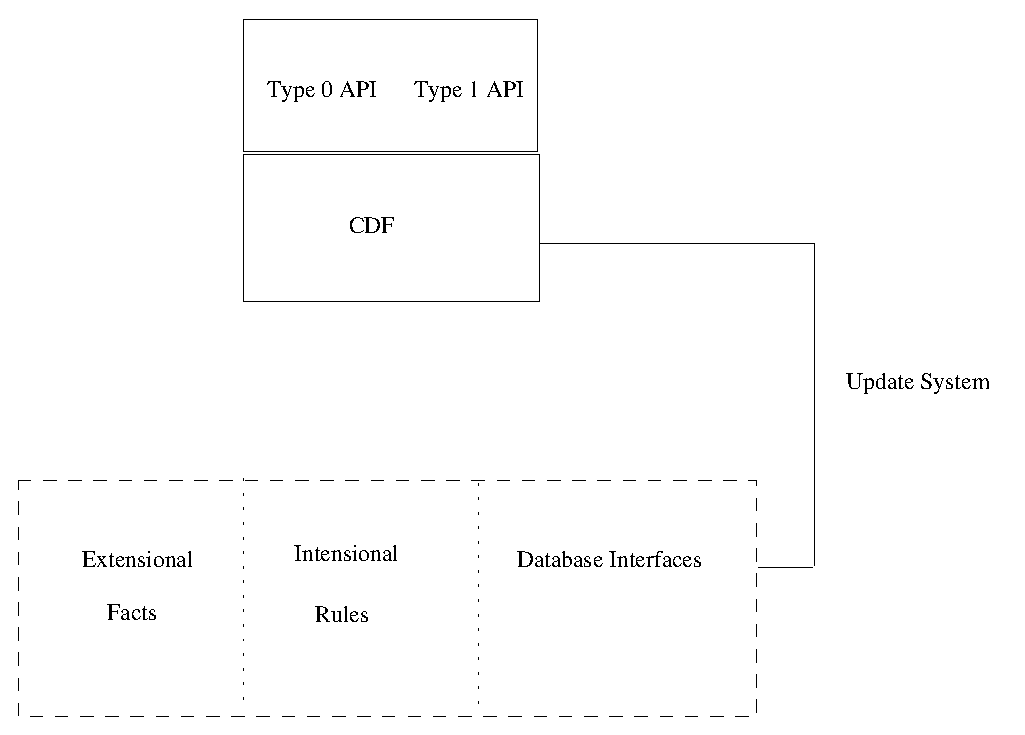
\epsfig{file=Figures/arch.eps,width=0.80\textwidth}}
%\caption{A High-Level Architecture of CDF and XJ}
%\label{fig:arch}
%\end{figure}
%--------------

CDF instances can be classified either as Type-0 or a Type-1, each of
which has its own interface.  Type-0 instances are useful for storing
large amounts of information; and consistency and implication in
Type-0 instances is computable in polynomial time.  Type-0 instances
describe classes by existential and universal relations, qualified
number restrictions, and relational hierarchies, but descriptions omit
negation and disjunction. Type-0 instances also support a direct
product construction for objects and classes.  
\comment{
These product classes and objects can be useful for representing
certain types of non-binary relations, and are particularly useful for
incorporating knowledge represented as RDF facts \cite{}.  }
Information in Type-0 CDF instances is tightly coupled to XSB's
query mechanism, and CDF ensures that only the most specific answers
(according to a given inheritance hierarchy) are returned for any
Type-0 query.

Type-1 instances extend Type-0 instances to describe classes using
negation and disjunction, and thus permit descriptions that are
equivalent to an expressive description logic.  In fact, a Type-1 CDF
instance can be seen as a knowledge base in which various classes are
described via {\em class expressions}, which correspond to formulas in
description logics.  Reasoning in Type-1 instances is done via the CDF
theorem-prover.  Using the Type-1 API, users may ask whether a given
class or object is consistent, whether a given class expression is
consistent with a class or object; or whether a given class expression
is entailed by a given class or object.  The problems of determining
consistency or entailment of a Type-1 class expression have a high
degree of complexity.  To solve these problems the CDF theorem prover
uses several heuristics, but a determined (or unlucky) user can always
find class expressions that requires a lot of time to check.

Of course, ontology management systems require many features in
addition to reasoning and representation features \cite{MGPS03}.  We
mention some of these features.

\begin{itemize}
\item {\em A Semantic Checking System}.  CDF has various mechanisms for
ensuring consistency of objects and classes both at the Type-0 or
Type-1 level.  Various levels of consistency can be checked during
various operations on the CDF instance.
%
\item {\em A Component System}. Reusability of ontologies is supported
by the {\em component} structure of CDF.  An ontology component may be
maintained by separate users or organizations in different locations
and assembled in various ways by applications.
%
\item {\em A Concurrency System}. (Not open-source) Based on the
component structure, the {\em concurrency} mechanism for CDF allows
users to update their own CDF instances and to periodically update a
common store. Naturally, the various mechanisms in CDF for ensuring
consistency that are vital to ensuring coherency when users update
their systems concurrently.
%
\item {\em Database Interfaces}. (Non open-souce) CDF supports various
interfaces to databases so that CDF facts can be stored in a database
or mapped to database tables.
\end{itemize}

Based on these features, CDF can support user interfaces in a number
of ways.  One of the most convenient is to use a XSB/Java interface
such as InterProlog~\cite{Cale01} or JAXSB~(see
\texttt{http://xsb.sourceforge.net}) and then write a user interface in
Swing or some other Java Graphics library.  One of the easiest ways to
do this is to make use of the {\em XJ system} which allows Swing Gui
objects to be represented as Prolog terms (the XJ system is non
open-source) From a systems perspective, a graphical interface is then
written XJ library Swing widgets or specialized XJ-CDF Swing widgets.
CDF per-se has the following graphical packages and applications.
%
\begin{itemize}
%
\item {\em An XJ Caching System}. Adds and deletes to CDF are extended
with a notification mechanism so that Java Swing objects (created with
XJ, XSB's graphics system) reflect the state of CDF even when it
dynamically changes.
%
\item {\em A Visual Editor}. Finally,  CDF supports a graphical editor
that allows users both to visualize an ontology and to perform the
functions mentioned so far.
\end{itemize}
%
Extensional facts, intensional rules, updates, the Type-0 and Type-1
interfaces, consistency checking predicates and the full component
system are available as an open-source package for XSB.  Other
features, concurrency mechanisms, specialized database interfaces, XJ
support and the editor are not yet open-source, but are included in
this manual to indicate the types of applications that can be
constructed with CDF.

%-----------------------------------------------------------
\section{The Meaning of Type-0 CDF Instances} \label{sec:type0} 

Facts in both Type-0 and Type-1 CDF instances are closely related to
class expressions in description logics.  However, because CDF often
stores class expressions as Prolog facts in an unconventional way, and
because description logics may not be familiar to a logic programming
audience, we present here a somewhat formal introduction to how CDF
represents knowledge.  Users without a mathematical background can
ignore the various axioms and formal definitions that are presented in
this chapter.  Our approach is to introduce a semantics of CDF based
on a translation of a {\em CDF instance} into a set of first-order
logic sentences that constitute an {\em Ontology Theory} whose models
are the models of a CDF instance.  For simplicity of presentation the
description of CDF instances in this section omits certain details
about components, extensional facts and intenstional rules, and other
topics that will be introduced in later chapters.

We illustrate aspects of CDF by means of an example drawn from
electronic commerce.  Health care organizations, such as hospitals,
clinics, etc., sometimes have difficulties in buying disposable
medical devices such as sutures, bandages, gloves, and so on.  These
difficulties arise from the fact that these devices may be quite
specialized: for instance some sutures are used only for particular
type of surgery on a particular organ.  At the same time, since these
devices are disposable, they may need to be purchased frequently.  We
consider concretely the class of {\em absorbable sutures}, which are
used for stitching and securing tissues, and which can be absorbed by
the human body.  Information below is adapted from he U.S. Defence
Logistics Information Service \url{http://www.dlis.mil}, from the
Universal Standard Products and Services Classification~\cite{UNSPSC},
as well as from websites of various commercial medical supply
companies.

\subsection{Type-0 CDF Instances} \label{sec:type0} 

We begin with the syntax of Type-0 instances~\footnote{The syntax for
  identfiers is simplified here, and differs in the actual CDF
  implementation. See Section~\ref{sec:instance}.}:

\begin{definition}[Type-0 Instances: Semantic Level] \label{def:ids}
A {\em Type-0 CDF instance} is a finite set of ground facts for the
predicates \pred{isa/2}, \pred{hasAttr/3}, \pred{allAttr/3},
\pred{classHasAttr/3}, \pred{minAttr/4}, and \pred{maxAttr/4}.  An {\em
identifier} is either a constant or a term.  The arguments of these
predicates are {\em concrete identifiers}, where a term $T$ is an
identifier iff $T$ has the functor symbol {\tt cid/1}, {\tt oid/1},
{\tt rid/1}, or {\tt crid/1} whose argument is either

\begin{enumerate}
\item a constant; or 
\item a term $f(I_1,\ldots,I_n)$ where $I_1,\ldots,I_n$ are identifiers.
\end{enumerate}
In the first case, an identifier is called {\em atomic}; in the second
it is called a {\em product identifier}.
\end{definition}

Despite the simple syntax of Type-0 CDF instances, their semantics
differs from the usual semantics assigned to facts in Prolog.
Identifiers identify sets of objects, or binary relations between
objects.  Furthermore, the facts of a Type-0 CDF instance can
implicitly denote inheritance of various relationships among classes
and objects, as well as inheritance constraints about what
relationships are allowed.

\subsection{Simple Taxonomies in CDF}

\begin{example} \rm \label{ex:suture1}
The following CDF instance illustrates a fragment of a taxonomy for
medical equipment.
%-------------------------------------------
{\tt  {\small 
\begin{tabbing}
foo\=foo\=foo\=foo\=foo\=foo\=foooo\=foooooooooooooooo\=\kill
isa(cid(medicalEquipment),cid('CDF Classes'))  \\
\> isa(cid(woundCareProducts),cid(medicalEquipment)) \\
\> \> \>  isa(cid(suturesAndRelatedProducts),cid(woundCareProducts)) \\
\> \> \> isa(cid(sutures),cid(suturesAndRelatedProducts))  \\
\> \> \> \> isa(cid(absorbableSutures),cid(sutures))  \\
\> \> \> \> isa(cid(nonAbsorbableSutures),cid(sutures)) \\
\> \\
\> \> \>   isa(oid(sutureU245H),cid(absorbableSutures))  \\
\> \> \> \> \>   isa(oid(suture547466),cid(sutures)) 
\end{tabbing} }} 
%-------------------------------------------
\noindent
In CDF, sets of objects are termed {\em classes} to stress the
informality of its sets from the perspective of set theory, and class
identifiers have the functor {\tt cid/1}.  One can read the fact
\begin{verbatim}
      isa(cid(nonAbsorbableSutures),cid(sutures))
\end{verbatim}
as ``all elements in the class {\tt cid(nonAbsorbableSutures)} are
also in the class {\tt cid(sutures)}'' --- in other words, that {\tt
cid(nonAbsorbableSutures)} is a subclass of {\tt cid(sutures)}.
Object identifiers have the functor {\tt oid/1}, and denote classes
with cardinality 1, or {\em singleton classes}.  The fact
\begin{verbatim}
      isa(oid(sutureU245H),cid(absorbableSutures))
\end{verbatim}
can be read as ``the element of the singleton class {\tt
oid(sutureU245H)} is in the class {\tt cid(absorbableSutures)}''.
Note that {\tt cid(absorbableSutures)} is (potentially) more specific
than the class {\tt cid(sutures)}, to which {\tt oid(suture547466)}
belongs.  The class {\tt cid('CDF Classes')} is taken to contain all
objects in the domain of discourse.  All identifiers in this simple
taxonomy are atomic.

The decision of whether to denote an entity as an object or as a class
depends on the use of a given CDF instance.  Here, a given part number
can specify a number of physical parts, but the physical parts are
taken to be identical for the purposes of this instance.  However, if
we were constructing a CDF instance for warehouse management, the
above objects might be better represented as classes, and the physical
objects represented as CDF objects.
\end{example} 

Implicit in the above example is the fact that we use the term {\em
object identifiers} or {\em objects} to denote singleton classes,
class identifiers to denote all classes (including singleton classes).
Elements cannot be denoted directly by CDF facts, but only through
singleton classes that contain them (and are isomorphic to them).  At
this point, we can begin defining the semantics of Type-0 CDF
instances.

%-------------------
\begin{definition} \label{def:ontolang}
\index{ontology language} \index{ontology structure} \index{ontology
theory}
%
An {\em ontology language} is a first-order language with equality
containing the predicates: {\em isClass/1, isElt/1, isRel/1, isCrel/1,
elt/2, rel/3, and crel/3}, and a countable set of constants.  An {\em
ontology structure} is a structure defined over an ontology language.
An {\em ontology theory} is a set of first-order sentences formed over
an ontology language that includes a set of {\em core axioms}, defined
below, along with the defined predicate:
\[
isObj(X) =_{def} isClass(X) \wedge 
	((elt(E_1,X) \wedge elt(E_2,X)) \Rightarrow E_1 = E_2)
\]
If $\cT$ is an ontology theory formed over an ontology
language $\cL$, an ontology structure $S$ over $\cL$ is a model of
$\cT$ if every sentence of $\cT$ is satisfied in $S$.
\end{definition}
%-------------------

\index{sorting predicates}
By convention we assume that the variables in an ontology language are
indexed by the set of natural numbers.  In this paper we will restrict
our attention to ontology languages whose constant and function
symbols are identifiers as described in Definition~\ref{def:ids}.
Informally $isClass/1$ indicates that an identifier $I$ is a class
name or {\em class identifier}; $isElt/1$ indicates that an identifier
$I$ is an element of a class; $isRel/1$ that $I$ is a {\em relation
identifier}; and $isCrel/1$ that $I$ is a {\em class-relation
identifier}; and $isObj/1$ that $I$ is an {\em object identifier}.  We
sometimes call these 5 predicates {\em sorting predicates}.
$elt(E,C)$ indicates that an element $O$ is a member of class
identifier $C$; $rel(O_1,R,O_2)$ indicates that an element $E_1$ has a
$R$ relation to an element $E_2$; and $crel(C_1,R,E)$ indicates that
the class identifier $C_1$ has a $R$ relation to an object identifier
$E$.

The first core axiom ensures that objects, classes, relations and
class-relations all have distinct identifiers within an ontology
language.
%-----------
\begin{axiom}[Distinct Identifiers] \label{ax:distinct}
\index{axioms!distinct identifiers} 
\ \\
\begin{tabbing}
foo\=foo\=foo\=foo\=foo\=foo\=foooo\=foooooooooooooooo\=\kill
\> $\neg \exists Id [isClass(Id) \wedge (isElt(Id) \vee isRel(Id) 
	                                 \vee isCrel(Id))] \wedge $ \\
\> $\neg \exists Id [isObj(Id) \wedge (isElt(Id) \vee isCrel(Id))] \wedge $ \\
\> $\neg \exists Id [isElt(Id) \wedge isCrel(Id)] $ 
\end{tabbing}
\end{axiom} 
%-----------

$isClass/1$, $isElt/1$, $isRel/1$, and $isCrel/1$ provide an effective
sorting that extends to all predicates, as the next axiom indicates.

\begin{axiom}[Predicate Sorts] \rm \label{ax:sorts}
\index{axioms!predicate sorts} 
\ \\
\begin{tabbing}
foo\=foo\=foo\=foo\=foo\=foo\=foooo\=foooooooooooooooo\=\kill
\> \> $(\forall X,Y) [elt(X,Y) \Rightarrow (isElt(X) \wedge isClass(Y))]
								\wedge $ \\
\> \> $(\forall X,Y,Z) [rel(X,Y,Z) \Rightarrow (isElt(X) \wedge isRel(Y)
					   \wedge isElt(Z))] \wedge  $ \\
\> \> $(\forall X,Y,Z) [crel(X,Y,Z) \Rightarrow (isClass(X) \wedge isRel(Y)
					   \wedge isElt(Z))] $ \\
\end{tabbing}
\end{axiom} 

%-----------

The following definition of $IdSort$ relates the functors of
identifiers in a Type-0 CDF instance to their sort in an ontology
theory.  It will be used in the various instance axioms to enforce
proper sorting of product identifiers.

\begin{definition}{\bf [IdSort]} \label{def:IdSort}
Let {\em I} is be an identifier. Then {\em IdSort(I)} is equal to {\em
isClass(I)} if the main functor symbol of {\em I} is {\tt cid/1}; {\em
isObj(I)} if the main functor symbol of {\em I} is {\tt oid/1}; {\em
isRel(I)} if the main functor symbol of {\em I} is {\tt rid/1}; and
{\em isCrel(I)} if the main functor symbol of {\em I} is {\tt crid/1}.
\end{definition}

%-----------------------------------------------------------------------------------------
\comment{
\begin{definition}{\bf [IdSort]}  Let {\em I} is be an identifier, and
$\cI$ be the set of identifiers occurring in {\em I}. Then
%
\[ IdSort(I) =_{def} \bigwedge_{I' \in \cI} Sort(I') \]
%
where {\em Sort(I)} is equal to {\em isClass(I)} if the main functor
symbol of {\em I} is {\tt cid/1}; {\em isObj(I)} if the main functor
symbol of {\em I} is {\tt oid/1}; {\em isRel(I)} if the main functor
symbol of {\em I} is {\tt rid/1}; and {\em isCrel(I)} if the main
functor symbol of {\em I} is {\tt crid/1}.
\end{definition}
}
%-----------------------------------------------------------------------------------------

From Definitions~\ref{def:IdSort} and~\ref{def:ontolang}, it is easy
to see that for any object identifier $O$, $IdSort(O) = isObj(O)$, and
$isObj(O) \Rightarrow isClass(O)$.

%-----------
\begin{instance} [Translation of {\tt isa/2}] \rm 
For each fact of the form {\tt isa(Id$_1$,Id$_2$)} add the axiom
\ \\
\begin{tabbing}
foo\=foo\=foo\=foo\=foo\=foo\=foooo\=foooooooooooooooo\=\kill
\> $ IdSort(Id_1) \wedge IdSort(Id_2) \wedge $ \\

\> \> $ (((isClass(Id_1) \wedge isClass(Id_2)) \wedge
	(\forall X) [elt(X,Id_1) \Rightarrow elt(X,Id_2)]) \vee $ \\

%\> \> $ ((isObj(Id_1) \wedge isClass(Id_2)) \wedge elt(Id_1,Id_2)) \vee $ \\

\> \> $ ((isRel(Id_1) \wedge isRel(Id_2)) \wedge
	(\forall X,Y)[rel(X,Id_1,Y) \Rightarrow rel(X,Id_2,Y)]) \vee $ \\

\> \> $ ((isCrel(Id_1) \wedge isCrel(Id_2)) \wedge
	(\forall X,Y)[crel(X,Id_1,Y) \Rightarrow crel(X,Id_2,Y)])) $ 
\end{tabbing}
denoted as {\tt isa(Id$_1$,Id$_2$)}$^{\cI}$.
\end{instance}
%-----------

Note that the reflexive and transitive closure of {\tt isa/2} is an
immediate consequence of its translation rule.  The next axiom is
technical.  It is important for the semantics of relations that each
class have at least one member.
%-----------
\begin{axiom}[Non-Empty Classes] \label{ax:nonnull}
\index{axioms!non-empty classes} 
\[ (\forall X) [isClass(X) \Rightarrow (\exists Y) [elt(Y,X)]] \]
\end{axiom} 
%-----------

The last core axiom for these predicates ensures is that each class is
a subclass of {\tt cid('CDF Classes')}.

%-----------
\begin{axiom}[Domain Containment] \label{ax:contained}
\index{axioms!domain containment} 
\[ (\forall X) [isElt(X) \Rightarrow elt(X,cid('CDF\ Classes'))] \]
\end{axiom} 
%-----------

\subsection{General Relations between Objects in  Classes}

\begin{example} \rm \label{ex:suture2}
The class {\tt cid(sutures)} can be further defined by its relations
to other classes.  For instance, an object in {\tt cid(sutures)} may
have a designation of its needle design indicating whether it is to be
used for abdominal surgeries, thoracic surgeries, or other purposes.
This information is indicated by the following CDF facts:
%
{\small
\begin{tabbing}
fooo\=foo\=foo\=foo\=fooooooooooooooooooooooooooooooo\=ooooooooooooo\=\kill
\> {\tt isa(rid(hasNeedleDesign),rid('CDF Relations'))} \\
\\
\> {\tt isa(cid(domainTypes),cid('CDF Classes'))} \\
\> \> {\tt isa(cid(needleDesignTypes),cid(domainTypes))} \\
\> \> \> {\tt isa(cid(Abdominal),cid(needleDesign))} \\
\> \> \> {\tt isa(cid(Abscisson),cid(needleDesign))} \\
\> \> \> {\tt isa(cid('Adson Dura'),cid(needleDesign))} \\
\> {\it \% 126 other values..}  \\
\\
\> {\tt allAttr(cid(sutures),rid(hasNeedleDesign),cid(needleDesign))} 
\end{tabbing}
}
%
\noindent
The {\tt allAttr/3} fact above can be read as ``if any object in {\tt
cid(absorbableSutures)} has a {\tt rid(hasNeedleDesign)} relation, it
must be to an object in the class {\tt cid(needleDesign)}''.  That
{\tt hasNeedleDesign} is a relation is indicated by clothing it in the
functor {\tt rid/1}.  This relation is an immediate subclass of all
{\tt CDF Relations} which in turn is taken to represent the universal
binary relation over the domain of discourse.  Thus the {\tt
allAttr/3} fact effectively types the range of {\tt
rid(hasNeedleDesign)} relations, stemming from objects in the class
{\tt cid(absorbableSutures)}, but it does not indicate the existence
of such a relationship.  From a user's point of view, the {\tt
rid(hasNeedleDesign)} relation can be thought of as an optional
attribute for a given {\tt cid(absorbableSutures)} object.  Sample
values for {\tt cid(hasNeedleDesignTypes)} are also given.
\end{example} 

%-------------------

{\tt allAttr/3} provides a simple but powerful mechanism for
inheritance of typing among CDF classes:
%---------------------------------------------------------------------------
\comment{
, as can be seen from the
following translation rule, which uses the defined formula

\[ 
elt(X,Y) =_{def} ((isClass(Y) \wedge elt(X,Y)) \vee (isObj(Y) 
			\wedge X = Y))
\] }
%---------------------------------------------------------------------------

\begin{instance} [Translation of {\tt allAttr/3}] \rm 
For each fact of the form {\tt allAttr(Id$_1$,Rid,Id$_2$)} add the instance
axiom: 
\begin{tabbing}
foo\=foo\=foo\=foo\=foo\=foo\=foooo\=foooooooooooooooo\=\kill
\> $ IdSort(Id_1) \wedge IdSort(Rid) \wedge IdSort(Id_2) \wedge $ \\
\> \> $ IsClass(Id_1) \wedge IsRel(Rid) \wedge IsClass(Id_2) \wedge $ \\
\> \> $(\forall X, Y) [(elt(X,Id_1) \wedge rel(X,Rid,Y))
					\Rightarrow elt(Y,Id_2)] $
\end{tabbing}
denoted as {\tt allAttr(Id$_1$,Rid,Id$_2$)$^{\cI}$}.
\end{instance}

%----------------------
\comment{
\begin{tabbing}
foo\=foo\=foo\=foo\=foo\=foo\=foooo\=foooooooooooooooo\=\kill
\> $ IdSort(Id_1) \wedge IdSort(Rid) \wedge IdSort(Id_2) \wedge $ \\
\> \> $ (IsClass(Id_1) \vee isObj(Id_1)) \wedge IsRel(Rid) \wedge 
	 (IsClass(Id_2) \vee isObj(Id_2)) \wedge $ \\
\> \> $(\forall X, Y) [(elt(X,Id_1) \wedge rel(X,Rid,Y))
					\Rightarrow elt(Y,Id_2)] $
\end{tabbing}
}
%----------------------
\begin{example} \rm \label{ex:hasAttr}
While {\tt allAttr/3} indicates a typing for relations, it does not
indicate that a relation must exist for elements of a class.  This
statement is made by \pred{hasAttr/3}.  The relation {\tt
rid(hasPointStyle)} for the class {\tt cid(absorbableSutures)} is
taken to be required in this schema.  The facts
%
{\small
\begin{tabbing}
fooo\=foo\=foo\=foo\=foooooooooooooooooooooooooooo\=ooooooooooooo\=\kill
\> {\tt allAttr(cid(absorbableSutures),rid(hasPointStyle),cid(pointStyle)) } \\
\> {\tt hasAttr(cid(absorbableSutures),rid(hasPointStyle),cid(pointStyle)) }
\end{tabbing}
}
%
\noindent
indicate not only the range of such relationships, but that such a
relationship must exist.  Indeed, the {\tt hasAttr/3} fact can be read
as ``all objects in the class {\tt cid(absorbableSutures)} have a
relation {\tt rid(hasPointStyle)} to an object in the class {\tt
cid(pointStyle)}''.  The facts below also give information about the
{\tt rid(hasPointStyle)} relation.
%
{\small
\begin{tabbing}
fooo\=foo\=foo\=foo\=foooooooooooboooooooooooooooo\=ooooooooooooo\=\kill
\> {\tt isa(cid(pointStyle),cid(domainTypes))} \\
\> {\tt isa(cid(regularCuttingEdge),cid(pointStyle))} \\
\> {\tt isa(cid(reverseCuttingEdge),cid(pointStyle))} \\
\> {\tt isa(cid(scalpelPoint),cid(pointStyle))} \\
\> {\it \% 10 other values.} \\
\\
\> {\tt hasAttr(oid(sutureU245H),rid(hasPointStyle),cid(regularCuttingEdge))}
\end{tabbing}
} 
\noindent
The last of the above facts can be read as ``the object {\tt
oid(sutureU245H)} has a {\tt rid(hasPointStyle)} relation to an object
in the class {\tt cid(pointStyle)}''.  
\end{example}

Not surprisingly, the definition of {\tt hasAttr/3} bears some
similarity to that of {\tt allAttr/3}.

\begin{instance} [Translation of \pred{hasAttr/3}] \rm 
For each fact of the form {\tt hasAttr(Id$_1$,Rid,Id$_2$)} add the instance
axiom: 
\begin{tabbing}
foo\=foo\=foo\=foo\=foo\=foo\=foooo\=foooooooooooooooo\=\kill
\> $ IdSort(Id_1) \wedge IdSort(Id_2) \wedge IdSort(Id_2) \wedge $ \\
\> \> $ IsClass(Id_1) \wedge IsRel(Rid) \wedge
	 IsClass(Id_2) \wedge $ \\
\> \> \> $ (\forall X) [elt(X,Id_1) \Rightarrow \exists Y [rel(X,Rid,Y) 
					\wedge elt(Y,Id_2)]]$
\end{tabbing}
denoted as {\tt hasAttr(Id$_1$,Rid,Id$_2$)$^{\cI}$}.
\end{instance}

We next turn to relational axioms that indicate the cardinality of
various relations.

\begin{example} \rm  \label{ex:maxAttr}
For our purposes, an object in {\tt cid(absorbableSutures)} can be
thought of as consisting of a needle and a thread~\footnote{The thread
is often called a suture.  We are assuming for purposes of
illustration that all sutures are --- in suture-speak --- ``armed''.}.  This is
represented by the facts:
%
{\small
\begin{tabbing}
foo\=foo\=foo\=foo\=foo\=foo\=foooo\=foooooooooooooooo\=\kill
\> {\tt allAttr(cid(absorbableSutures),rid(hasImmedPart),cid(absSutPart)) } \\
\> {\tt hasAttr(cid(absorbableSutures),rid(hasImmedPart),cid(absSutNeedle)) } \\
\> {\tt hasAttr(cid(absorbableSutures),rid(hasImmedPart),cid(absSutThread)) } \\
\\
\> {\tt isa(cid(absSutPart),cid(suturesAndRelatedProducts))}  \\
\> \> {\tt isa(cid(absSutNeedle),cid(absSutPart)) } \\
\> \> {\tt isa(cid(absSutSuture),cid(absSutPart)) } 
\end{tabbing}
}
%
\noindent
A needle for an absorbable suture is typically made of a different
material than the thread to which the needle is attached.  Each of
these materials may be important in choosing an absorbable suture, and
each of these materials are unique.  The facts
%
{\small
\begin{tabbing}
foo\=foo\=foo\=foo\=foo\=foo\=foooo\=foooooooooooooooo\=\kill
\> {\tt hasAttr(cid(absSutPart),rid(hasMaterial),cid(absSutMaterial)) } \\
\> {\tt maxAttr(cid(absSutPart),rid(hasMaterial),cid(absSutMaterial),1) } \\
\\
\> {\tt isa(cid(material),cid(domainTypes))} \\
\> {\tt isa(cid(absSutMaterial),cid(material)} \\
\> {\tt isa(cid(gut),cid(absSutMaterial))} \\
\> {\tt isa(cid(polyglyconate),cid(absSutMaterial))} \\
\> {\tt isa(cid(polyglyconicAcid),cid(absSutMaterial)) } 
\end{tabbing}
}
%
\noindent
indicate that each {\tt cid(absSutPart)} has a unique material.  The
{\tt maxAttr/4} fact can be read as ``Each object in the class {\tt
cid(absSutPart)} has at most 1 {\tt rid(hasMaterial)} relation to an
object in the class {\tt cid(absSutMaterial)}''.
\end{example}

In order to define the semantics of {\tt maxAttr/4}, let
$\exists^{\leq n}X_m[ \phi(X,Z)]$ be defined as an abbreviation for
the formula
\[
  \exists x_m,...,\exists x_{m+n} [\bigwedge_{m \leq i \leq m+n} 
	\phi(x_i,\overline{z}) 
	\Rightarrow \bigvee_{m \leq i < j \leq m+n} x_i  = x_j]
\]
i.e., for the formula indicating that there are at most $N$ non-equal
elements satisfying $\phi(x,z)$.  The abbreviation $\exists^{\geq N}$
is defined similarly to indicate that a formula is satisfied by at
least $N$ non-equal elements.

\begin{instance} [Translation of {\tt maxAttr/4}] \rm 
For each fact of the form {\tt maxAttr(Id$_1$,Rid,Id$_2$,N)} add the instance
axiom: 
\begin{tabbing}
foo\=foo\=foo\=foo\=foo\=foo\=foooo\=foooooooooooooooo\=\kill
\> $ IdSort(Id_1) \wedge IdSort(Id_2) \wedge IdSort(Id_2) \wedge $ \\
\> \> $ IsClass(Id_1) \wedge IsRel(Rid) \wedge
	 (IsClass(Id_2) \wedge $ \\
\> \> \> $ (\forall X) [elt(X,Id_1) \Rightarrow \exists^{\leq N} Y [rel(X,Rid,Y) 
					\wedge elt(Y,Id_2)]]$
\end{tabbing}
denoted as {\tt maxAttr(Id$_1$,Rid,Id$_2$,N)$^{\cI}$}.
\end{instance}

A corresponding predicate, {\tt minAttr/4} is used to indicate a
minimality restriction on a relation.  {\tt minAttr/4} is defined
similarly to {\tt maxAttr/4}, but using $\exists^{\geq N}$ rather than
$\exists^{\leq N}$.  Indeed, the predicate
%
{\small {\tt 
\begin{tabbing}
foo\=foo\=foo\=foo\=foo\=foo\=foooo\=foooooooooooooooo\=\kill
\> hasAttr(cid(absSutPart),rid(hasMaterial),cid(absSutMaterial)).
\end{tabbing}
} }
%
\noindent
could be replaced by the predicate
%
{\small {\tt 
\begin{tabbing}
foo\=foo\=foo\=foo\=foo\=foo\=foooo\=foooooooooooooooo\=\kill
\> minAttr(cid(absSutPart),rid(hasMaterial),cid(absSutMaterial),1).
\end{tabbing}
} }
%
\subsection{Class Relations}
Each of the predicates discussed so far are inheritable in their first
argument.  For instance, the fact
{\small {\tt 
\begin{tabbing}
foo\=foo\=foo\=foo\=foo\=foo\=foooo\=foooooooooooooooo\=\kill
\> hasAttr(cid(absSutPart),rid(hasMaterial),cid(absSutMaterial)).
\end{tabbing}
} } 
%
\noindent
implies that every subclass of {\tt cid(absSutures)} will have a
material in the class {\tt cid(absSutMaterial)}.  However, classes may
have relations that do {\em not} hold for their subclasses or members.
For instance, a finite set may have a given cardinality, but its
proper subsets will have a different cardinality.  Such relations are
termed {\em class relations}.

%-------------------
\begin{example} \label{ex:strel} \rm 
A practical example of a class relation comes from an application that
may be called part equivalency matching.  In this application, the
possible attributes for a class of parts are given various weights.
Two parts match if the sum of the weights of their attributes that
match are above a given threshold.  The weighting for the {\tt
cid(pointStyle)} of sutures might be given as:
%----------------------------------
{\small 
{\tt 
\begin{tabbing}
foo\=foo\=foo\=foo\=foo\=foo\=foooo\=foooooooooooooooo\=\kill
\> isa(cid(pointStyleWeight),cid('CDF Classes')) \\
\> \> isa(cid(highWeight),cid(pointStyleWeight)) \\
\> \> isa(cid(lowWeight),cid(pointStyleWeight)) \\
\\
\> classHasAttr(cid(sutures),crid(pointStyleWeight),cid(highWeight))
\end{tabbing}
} }
%----------------------------------
\noindent
The {\tt classHasAttr/3} fact can be read as ``the class {\tt
cid(sutures)} has a {\tt crid(pointStyleWeight)} relation to an object
in {\tt cid(highWeight)}.  Matching weights are made non-inheritable
via {\tt classHasAttr/3} because a weight may depend on a given
classification of a part.  For instance if a part were classified as a
{\tt cid(nonAbsorbableSuture)}, its {\tt cid(pointStyle)} might weigh
less (or more) for determining whether two sutures are equivalent.
\end{example}
%------------------
\begin{instance} [Translation of {\tt classHasAttr/3}] \rm 
For each fact of the form {\tt classHasAttr(Id$_1$,CRid,Id$_2$)} add the
instance axiom: 
\begin{tabbing}
foo\=foo\=foo\=foo\=foo\=foo\=foooo\=foooooooooooooooo\=\kill
\> $ IdSort(Id_1) \wedge IdSort(CRid) \wedge IdSort(Id_2) \wedge $ \\
\> \> $ IsClass(Id_1) \wedge IsCrel(CRid) \wedge isClass(Id_2) \wedge $ \\
\> \> \> $ (\exists X) [elt(X,Id_2) \wedge crel(Id_1,CRid,X)] $
\end{tabbing}
denoted as {\tt classHasAttr(Id$_1$,Rid,Id$_2$)$^{\cI}$}.
\end{instance}
%----------

\subsection{Product Classes}

The above predicates allow the definition of various named binary
relations between classes.  However, binary definitions can sometimes
be inconvenient to use.  For instance, in the part equivalency
matching example, (Example~\ref{ex:strel}), it may be desirable to
make explicit the weight of the match as an indication of the strength
of the match.  The weight could be made explicit by a series of
definitions
%-------------------------------------------
{\small 
{\tt 
\begin{tabbing}
foo\=foo\=foo\=foo\=foo\=foo\=foooo\=fooooooooooooooo\=\kill
\> allAttr(\cid{dlaPart},\rid{suturesRusMatch\_low},\cid{suturesRusPart}) \\
\> : \\
\> allAttr(\cid{dlaPart},\rid{suturesRusMatch\_high},\cid{suturesRusPart})
\end{tabbing}
} } 
%----------------------------------
\noindent
indicting that a given part has a match of weight {\em low} through
{\em high}.  However, for a scale with a large number of values,
defining matches in this way is time-consuming and prone to errors.
To address this, we first define a new class {\tt \cid{matchScale}}
containing as subclasses the various match levels.  We then combine
{\tt \cid{matchScale}} with the class {\tt \cid{suturesRusPart}} in a
product with a {\em product identifier}, as in the following fact
%-------------------------------------------
{\small 
{\tt 
\begin{tabbing}
foo\=foo\=foo\=foo\=foo\=foo\=foooo\=foooooooooooooooo\=\kill
 
allAttr(\cid{dlaPart},\rid{suturesRusMatch}, \\
\> \> \> \> \cid{partMach(\cid{suturesRusPart},\cid{matchScale})})
\end{tabbing}  } }
\noindent 
which indicates that a {\tt \cid{dlaPart}} can have a {\tt
\cid{suturesRusMatch}} to an object in the {\tt partMatch/2}  class,
which has both a {\tt \cid{suturesRusPart}} component and a {\tt
\cid{matchScale}} component.

%-------------------------------------------------------------------

We capture the intuition behind product classes through the following
axiom schemas.  The first indicates that product identifiers 
are constructed from {\em constituent identifiers} of the same sort.

\begin{axiom}[Downward Closure] \label{ax:downcl}
\index{axioms!downward closure}
\ \\
For each product identifier $\cid{f(x_1,\ldots,x_n)}$,
$\oid{f((x_1,\ldots,x_n)}$, $\rid{f(x_1,\ldots,x_n)}$, and
$c\rid{f((x_1,\ldots,x_n)}$ the following axiom is added,
\begin{tabbing}
foo\=foo\=foo\=foo\=foo\=foo\=foooo\=foooooooooooooooo\=\kill
\> $isClass(\cid{f(x_1,\ldots,x_n)}) \Rightarrow 
	isClass(x_1) \wedge \ldots \wedge isClass(x_n) $\\
\> $isObj(\oid{f(x_1,\ldots,x_n)}) \Rightarrow 
	isObj(x_1) \wedge \ldots \wedge isObj(x_n) $\\
\> $isRel(\rid{f(x_1,\ldots,x_n)}) \Rightarrow 
	isRel(x_1) \wedge \ldots \wedge isRel(x_n) $\\
\> $isCrel(\crid{f(x_1,\ldots,x_n)}) \Rightarrow 
	isCrel(x_1) \wedge \ldots \wedge isCrel(x_n) $
\end{tabbing}
\end{axiom}

With this axiom, along with the use of $IdType/1$ in the various
instance axioms, we will sometimes refer to a CDF identifier $I$ as a
class identifier if its outer functor is {\tt cid/1}, an object
identifier if its outer functor is {\tt oid/1} etc.  The next axiom
associates product classes with the objects they contain.

\begin{axiom}[Implicit Subclassing] \label{ax:implsc}
\index{axioms!implicit subclassing} 

\begin{enumerate}
\item For each product identifier $cid(f(x_1,\ldots,x_n))$ or 
$oid(f(x_1,...,x_n))$, the following axioms are added for $x_i, 1 \leq i
\leq n$:
\[
(\forall E) [(elt(E,y_i) \Ra elt(E,x_i)) \Ra \\
	(\forall E') [elt(E',f(x_1,...x_n))[x_i/y_i] \Rightarrow elt(E',f(x_1,...x_n))]]
\]

\item For each product identifier $rid(f(x_1,\ldots,x_n))$ the
following axioms are added for $x_i, 1 \leq i 
\leq n$:
\begin{tabbing}
foo\=foo\=foo\=foo\=foo\=foo\=foooo\=foooooooooooooooo\=\kill
\> $(\forall E_1,E_2) [(rel(E_1,y_i,E_2) \Ra rel(E_1,x_i,E_2)) \Ra$ \\
\> \> $(\forall E'_1,E'_2) [rel(E'_1,f(x_1,...x_n),E'_2)[x_i/y_i] \Ra rel(E'_1,f(x_1,...x_n),E'_2)]]$
\end{tabbing}
\end{enumerate}
\end{axiom}

%-------------------------------------------
\comment{
\begin{axiom}[Implicit Subclassing] \label{ax:implsc}
\begin{enumerate}
\item For each product identifier $\oid{f(x_1,\ldots,x_n)}$ the
following axiom is added:  
\[(\forall O) [elt(O,\cid{f(x_1,\ldots,x_n)})
	\Ra (O = \oid{f(y_1,\ldots,y_n)} \wedge 
  		  elt(y_1,x_1) \wedge \ldots \wedge elt(y_n,x_n))] \]

\item For each product identifier $\cid{f(x_1,\ldots,x_n)}$ and for
each atomic identifier $\cid{c}$ the following axiom is
added:
\[ (\forall C) 
   ([elt(\oid{f(x_1,\ldots,x_n)},C)] \Ra (C = \cid{f(y_1,\ldots,y_n)}
   \vee C = \cid{c})) \]
\end{enumerate}
\end{axiom}
}
%-------------------------------------------

\begin{example} \rm
Axiom~\ref{ax:downcl} simply states that identifier types cannot be
mixed within a product identifier.  For instance, if {\tt
\oid{matchLevelN}} is an object in the {\tt \cid{matchScale}},
then the identifier 

{\tt \cid{partMatch(\cid{suturesRusMatch},\oid{matchLevelN})}}

\noindent
is improperly formed.  On the other hand, if {\tt \oid{sutureU245H}} is in
the class {\tt \cid{suturesRusPart}}, then the identifier {\tt
\oid{partMatch(\oid{sutureU245H},\oid{matchLevelN})}} is a product
identifier that is also an object identifier.

Axiom~\ref{ax:implsc} also means that the inheritance relation of a
product class is partly determined by the inheritance relation of its
constituent elements.
\end{example}

\comment{
Core Axiom~\ref{ax:implsc} can be used either to set up equality
constraints on a model of a CDF instance, or it can be used to
determine which CDF instances have free models (as explained in the
next section).  The following example illustrates the first use.

\begin{example} \rm \label{ex:equality}
Suppose we have the CDF instance
{\small 
{\tt 
\begin{tabbing}
foo\=foo\=foo\=foo\=foo\=foo\=foooo\=foooooooooooooooo\=\kill
\> isa(\cid{a},\cid{f(a)}.
\end{tabbing} } } 
\noindent
By Core Axiom~\ref{ax:nonnull} (Non-empty Classes), {\tt \cid{a}} has
at least one element, which can be called {\tt \oid{a1}}.  By the
instance axiom for the above fact, {\em elt(\oid{a1},\cid{f(a)}}.  By
Core Axiom~\ref{ax:implsc}(1), it must be the case that 
%
\[ \oid{a1} = \oid{f(Y)} \wedge elt(Y,\cid{a}) \]
%
If we take $Y = \oid{a1}$, then this means that 
%
$ \oid{a1} = \oid{f(\oid{a1})} $
% 
so that the above fragment has a model $\cM$ with a single individual
(in the universe of $\cM$) to which all object identifiers are mapped,
and that has a $elt/2$ relation to each individual to which a class
identifier is mapped (among other models).
\end{example}
}

%\input{models}

\section{Implementation and System Features} \label{sec:impl}
%
In this section we describe how the CDF system implements the
semantincs of Section~\ref{sec:type0} , as well as many other features
for ontology management.  We begin by describing CDF identifiers,
facts, and rules in Section~\ref{sec:instance}.  The Type-0 query
interface, based on tabled resolution is described in
Section~\ref{sec:type0query}.  Section~\ref{sec:type0query} describes
the Type-1 API, which is based on the CDF therorem prover.  Update and
consistency predicates for CDF are described in
Section~\ref{sec:update}.  Section~\ref{sec:config} describes how to
configure CDF, along with predicates that allow the user to examine
aspects of the CDF state.  Section~\ref{sec:components} describes
basic I/O for CDF, along with a more sophisticated {\em component}
system that is built on top of basic I/O.  Section~\ref{sec:database}
describes database interfaces for CDF, and
Section~\ref{sec:concurrency} describes concurrency support.

%----------------------------------------------------


\subsection{CDF Instances} \label{sec:instance}

Part~\ref{part:semantics} simplified the syntax of CDF instances in
certain ways.  In this section we describe those aspects of the actual
CDF implementation that differ from the abstract presentation
Part~\ref{part:semantics}.

The first major difference concerns CDF identifiers.

\index{CDF Identifer}
\index{component tag}
\begin{definition}[CDF Identifiers] \label{def:cdfids}
A {\em CDF identifier} has the functor symbol {\tt cid/2}, {\tt
oid/2}, {\tt rid/2}, or {\tt crid/2}.  The second argument of a CDF
identifier is a Prolog atom and is called its {\em component tag},
while the first argument is either
\begin{enumerate}
\item a Prolog atom or 
\item a term $f(I_1,\ldots,I_n)$ where $I_1,\ldots,I_n$ are CDF identifiers.
\end{enumerate}
In the first case, an identifier is called {\em atomic}; in the second
it is called a {\em product identifier}.
\end{definition}

Thus in an implementation of, say, Example~\ref{ex:suture1} all
identifiers would have component tags.  For instance the identifier
{\tt cid(absorbableSutures)} might actually have the form {\tt
cid(absorbableSutures,unspsc)} and {\tt oid(sutureU245H)} would have
the form {\tt oid(sutureU245H,sutureRus)}.  These component tags have
two main uses.  First, they allow ontolgies from separate soruces to
be combined, and thus function in a manner somewhat analogous to XML
namespaces.  Second, the component tags are critical to the CDF
component system, described in \secref{sec:components}.

%----------------------------------------------------------------------------
\subsubsection{Extensional Facts and Intensional Rules}

\index{extensional facts} \index{intensional rules}
%
An actual CDF instance is built up of {\em extensional facts} and {\em
intensional rules} defined for the CDF predicates {\tt isa/2} {\tt
allAttr/3}, {\tt hasAttr/3}, {\tt classHasAttr/3}, {\tt coversAttr/3},
{\tt minAttr/4} and {\tt maxAttr/4}.  Extensional facts for these
predicates add the suffix {\tt \_ext} to the suffix name leading to
{\tt isa\_ext/2}, {\tt allAttr\_ext/2} and so on.  Intensional rules
add the suffix {\tt \_int} leading to {\tt isa\_int/2}, {\tt
allAttr\_int/2} etc.

Extensional facts make use of XSB's sophisticated indexing of dynamic
predicates.  Since CDF Extensional Facts use functors such as {\tt
  cid/1} or {\tt oid/1} to type their arguments, traditional Prolog
indexing, which makes use only of the predicate name and outer functor
of the first argument, is unsuitable for large CDF instances.  CDF
extensional facts use XSB's star-indexing (cf. Volume 1 of this
manual).  For ground terms, star-indexing can index on up to the first
five positions of a specified argument.  In addition, various
arguments and combinations of arguments can be used with star-indexing
of dynamic predicates.  The ability to index within a term is critical
for the performance of CDF; also since star-indexing bears
similarities to XSB's trie-indexing~\cite{RRSSW98}, it is spatially
efficient enough for large-scale use.  Section~\ref{sec:config}
provides information on default indexing in CDF and how it may be
reconfigured.

Intensional rules may be defined as XSB rules, and may use any of
XSB's language or library features, including tabling, database, and
internet access.  Intensional rules are called on demand, making them
suitable for implementing functionality from lazy database access
routines to definitions of primitive types.

\begin{example} \rm \label{ex:intrules}
In many ontology management systems, integers, floats, strings and so
on are not stored explicitly as classes, but are maintained as a sort
of {\em primitive type}.  In CDF, primitive types are easily
implemented via intensional rules like the following.
%
{\small {\sf  
\begin{tabbing}
foo\=foo\=foooooooooooooooooooooooooooooooooooooooo\=foo\=\kill
%
\> isa\_int(oid(Float),cid(allFloats)):- \\
\> \> 	(var(Float) -$>$ cdf\_mode\_error ; float(Float). \\
\end{tabbing} } }
\end{example}
%
CDF provides intensional rules defining all Prolog primitive types as
CDF primitive types in the component \component{cdfpt} (see below).
Other, more specialized types can be defined by users by defining
intensional rules along the same lines {\sc fill in 'below'; tabling
and intensional rules}

As mentioned above, the predicate {\tt
immed\_hasAttr/3}, (and {\tt immed\_allAttr/3}, etc) is used to store
basic CDF information that is used by predicates implementing {\tt
hasAttr/3} and other relations.  {\tt immed\_hasAttr/3} itself is
implemented as:
%
{\small {\sf  
\begin{tabbing}
foo\=foo\=foooooooooooooooooooooooooooooooooooooooo\=foo\=\kill
%
\> immed\_hasAttr(X,Y,Z):- hasAttr\_ext(X,Y,Z). \\
\> immed\_hasAttr(X,Y,Z):- hasAttr\_int(X,Y,Z). \\
\> immed\_hasAttr(X,Y,Z):- immed\_minAttr(X,Y,Z,\_). 
\end{tabbing} } }
%
\noindent
The above code fragment illustrates two points.  First, {\tt
immed\_hasAttr/3} is defined in terms of {\tt immed\_minAttr/3},
fulfilling the semantic requirements of Section \ref{sec:type0}.
It also illustrates that {\tt immed\_hasAttr/3} is implemented in
terms both of extensional facts {\tt hasAttr\_ext/3} and intensional
rules {\tt hasAttr\_int(X,Y,Z)}.  

%-------------------------------------------

\subsubsection{The Top-level Hierarchy and Primitive Types}

All CDF instances share the same top-level hierarchy, as depicted in
Figure~\ref{fig:toplevel}.  All classes and objects are subclasses
(through the {\tt isa} relation) to {\tt cid('CDF Classes',cdf)}, all
relations are subrelations of {\tt rid('CDF Object-Object
Relations',cdf)} and all class relations are subrelations of {\tt
crid('CDF Class-Object Relations',cdf)}.
%-------------------------------------------
\index{identifiers!cid('CDF Classes',cdf)}
\index{identifiers!rid('CDF Object-Object Relations,cdf)}
\index{identifiers!crid('CDF Class-Object Relations',cdf)}
\index{identifiers!cid('CDF Primitive Types',cdf)}
\index{identifiers!cid(allIntegers,cdf)}
\index{identifiers!cid(allFloats,cdf)}
\index{identifiers!cid(allAtoms,cdf)}
\index{identifiers!cid(allStructures,cdf)}
\index{identifiers!cid(atomicIntegers,cdf)}

\begin{figure}[htb] 
{\small {\it
\begin{center}
\begin{bundle}{cid('CDF Classes',cdf)}
\chunk{\begin{bundle}{cid('CDF Primitive Types',cdf)}
  \chunk{\begin{bundle}{cid(allIntegers,cdf)\ \ \ \ \ \    }
	\chunk{oid(Integer,cdfpt)}
	\end{bundle} }
  \chunk{\begin{bundle}{cid(allFloats,cdf)\ \ \ \ \ \ }
	\chunk{oid(Float,cdfpt)}
	\end{bundle} }
  \chunk{\begin{bundle}{cid(allAtoms,cdf)\ \ \ \ \ \ }
	\chunk{oid(Atom,cdfpt)}
	\end{bundle} }
  \chunk{\begin{bundle}{cid(allStructures,cdf)\ \ \ \ \ \ }
	\chunk{oid(Structure,cdfpt)}
	\end{bundle} }
  \chunk{\begin{bundle}{cid(atomicIntegers,cdf)}
	\chunk{oid(AInteger,cdfpt)}
	\end{bundle} }
  \end{bundle} } 
\end{bundle}
\end{center}

\ \\
\begin{center}
rid('CDF Object-Object Relations',cdf)
\end{center}

\ \\
\begin{center}
\begin{bundle}{crid('CDF Class-Object Relations',cdf)}
\chunk{crid('Name',cdf)}
\chunk{crid('Description',cdf)}
\end{bundle}
\end{center}
} }
\caption{Built-in Inheritance Structure of CDF}
\label{fig:toplevel}
\end{figure}
%-------------------------------------------

An immediate subclass of {\tt cid('CDF Classes',cdf)} is {\tt cid('CDF
Primitive Types',cdfpt)}.  This class allows users to maintain in CDF
any legally syntactic Prolog element, and forms an exception to
Definition~\ref{def:cdfids}.  Specifically {\tt cid('CDF Primitive
Types',cdf)} contains Prolog atoms, integers, floats, structures and
what are termed ``atomic integers'' --- integers that are represented
in atomic format, e.g. '01234'.  Primitive types are divided into five
subclasses, {\tt cid(allIntegers,cdf)}, {\tt cid(allFloats,cdf)}, {\tt
cid(allAtoms,cdf)}, {\tt cid(allStructures,cdf)}, and {\tt
cid(atomicInteger,cdf)}.  Each of these in turn have various objects
as their immediate subclasses~\footnote{Recall that objects in CDF are
singleton classes.}, whose inheritance relation is defined by an
intensional rule like the one presented in Example~\ref{ex:intrules}.
Thus, if the number 3.2 needs to be added to an ontology, perhaps as
the value of an attribute, it is represented as {\tt oid(3.2,cdfpt)},
and it will fit into the inheritance hierarchy as a subclass of {\tt
cid(allFloats,cdf)}.  The intensional rules are structured so that for
any Prolog syntactic element {\tt X}, when {\tt X} is combined with
the component \component{cdfpt}, then {\tt cid(X,cdfpt)} will be a
subclass of {\tt cid('CDF Primitive Types',cdfpt)}, as will be {\tt
oid(X,cdfpt)}.

\subsubsection{Basic CDF Predicates}

\begin{description}
\ourpredmodrptitem{isa\_ext/2}{usermod}
\ourpredmodrptitem{allAttr\_ext/3}{usermod}
\ourpredmodrptitem{hasAttr\_ext/3}{usermod}
\ourpredmodrptitem{classHasAttr\_ext/3}{usermod}
\ourpredmodrptitem{minAttr\_ext/4}{usermod}
\ourpredmodrptitem{maxAttr\_ext/4)}{usermod}
%\ourpredmodrptitem{coversAttr\_ext/3)}{usermod}
\ourpredmoditem{necessCond\_ext/2)}{usermod}
%
These dynamic predicates are used to store extensional facts in CDF.
They can be called directly from the interpreter or from files that
are not modules, but must be imported from {\tt usermod} by those
files that are modules.  Extensional facts may be added to a CDF system
via \pred{newExtTerm/1} (\secref{sec:update}), or imported from a
\ttindex{cdf\_extensional.P} file (\secref{sec:components}).

\ourpredmodrptitem{isa\_int/2}{usermod}
\ourpredmodrptitem{allAttr\_int/3}{usermod}
\ourpredmodrptitem{hasAttr\_int/3}{usermod}
\ourpredmodrptitem{classHasAttr\_int/3}{usermod}
\ourpredmodrptitem{minAttr\_int/4}{usermod}
\ourpredmodrptitem{maxAttr\_int/4)}{usermod}
%\ourpredmodrptitem{coversAttr\_int/3)}{usermod}
\ourpredmoditem{necessCond\_int/2)}{usermod}
%
These dynamic predicates are used to store intensional rules in CDF.
They can be called directly from the interpreter or from files that
are not modules, but must be imported from {\tt usermod} by those
files that are modules.  Intensional rules may be added to a CDF
system via \pred{???newIntRule/1} (\secref{sec:update}), or imported from
a \ttindex{cdf\_intensional.P} file (\secref{sec:components}).


\ourpredmoditem{immed\_isa/2}{cdf\_init\_cdf}
{\tt immed\_isa(SubCid,SupCid)} is true if there is a corresponding
fact in \pred{isa\_ext/2} or in the intensional rules.  It does not
use the Implicit Subclassing Axiom \ref{ax:implsc}, the Domain
Containment Axiom~\ref{ax:contained}, or reflexive or transitive
closure.

\ourpredmodrptitem{immed\_allAttr/3}{cdf\_init\_cdf}
\ourpredmodrptitem{immed\_hasAttr/3}{cdf\_init\_cdf}
\ourpredmodrptitem{immed\_classHasAttr/3}{cdf\_init\_cdf}
\ourpredmodrptitem{immed\_minAttr/4}{cdf\_init\_cdf}
\ourpredmodrptitem{immed\_maxAttr/4)}{cdf\_init\_cdf}
%\ourpredmodrptitem{immed\_coversAttr/3)}{cdf\_init\_cdf}
\ourpredmoditem{immed\_necessCond/2)}{cdf\_init\_cdf}
Each of these predicates calls the corresponding extensional facts for
the named predicate as well as the intensional rules.  No inheritance
mechanisms are used, and any intensional rules unifying with the call
must support the call's instantiation pattern.


\ourpredmoditem{cdf\_id\_fields/4}{cdf\_init\_cdf}
{\tt cdf\_id\_fields(ID,Functor,NatId,Component)} is true if {\tt ID}
is a legal CDF identifier, {\tt Functor} is its main functor symbol,
{\tt NatId} is its first field and {\tt Component} is its second
field.  This convenience predicate provides a faster way to examine
CDF identifiers than using {\tt functor/3} and {\tt arg/3}.

\end{description}

`\section{The Type-0 Query Interface} \label{sec:type0query}

There are two main design goals behind the Type-0 query interface.
\begin{itemize}
\item to provide a Prolog interface to CDF based on  
the axioms in Chapter~\ref{sec:type0}, and the {\sc inh} proof system
derived from \refsec{sec:inheritance} along with
Proposition~\ref{prop:necesscondinh}.
\item to provide a highly efficient and scalable interface to CDF.
\end{itemize}

Indeed, the Type-0 interface has been used to support CDF instances
containing nearly a million extensional facts that require heavy
manipulation and access, and are used as back-ends to interactive
graphical systems.  As discussed below, this need for efficiency
affects certain aspects of the interface.

\subsection{Virtual Identifiers}
As discussed, Type-0 instances do not make contain facts of the form
\pred{necessCond/2}.  In the implementation of CDF, {\tt necessCond/2}
goals can be called, and their implementation obeys the first-argument
inheritance for {\tt necessCond}.  However, it is important to note
that {\bf the Type-0 interface does not use information in virtual
identifiers} as the following example shows.

\begin{example} \rm 
Consider the CDF instance containing only the fact
{\small 
{\tt 
\begin{tabbing}
foo\=foo\=foo\=foo\=foo\=foo\=foooo\=foooooooooooooooo\=\kill
\> necessCond\_ext(cid(a,test),vid(exists(rid(r,test),cid(b,test)))).
\end{tabbing} } } 
%
\noindent
by the semantics of type 1 ontologies, this CDF instance logically
entails {\small {\tt
\begin{tabbing}
foo\=foo\=foo\=foo\=foo\=foo\=foooo\=foooooooooooooooo\=\kill
\> hasAttr(oid(a,test),rid(r.text),cid(b,text))$^{\cI}$
\end{tabbing} } } 
%
\noindent
However the Type-0 interface will answer ``no'' to the query 
{\small 
{\tt 
\begin{tabbing}
foo\=foo\=foo\=foo\=foo\=foo\=foooo\=foooooooooooooooo\=\kill
\> ?- hasAttr(oid(a,test),rid(r.text),cid(b,text)).
\end{tabbing} } } 
%
\end{example}

\subsection{Computing Irredundant Answers}

Consider the running sutures example of Chapter~\ref{sec:type0} to
which is added a fact
%
{\small 
{\tt 
\begin{tabbing}
foo\=foo\=foo\=foo\=foo\=foo\=foooo\=foooooooooooooooo\=\kill
\> hasAttr(oid(sutureU245H),rid(needleDesign),cid('Adson Dura')).
\end{tabbing} } } 
%
\noindent
Suppose the query {\tt ?-
hasAttr(oid(sutureU245H),rid(needleDesign),Y)} were asked.  Via an
{\sc inh} proof, rhe CDF instance would imply the answers 
%
{\small {\tt
\begin{tabbing}
foo\=foo\=foo\=foo\=foo\=foo\=foooo\=foooooooooooooooo\=\kill
\>  hasAttr(oid(sutureU245H),rid(needleDesign),cid('Adson Dura')) \\
\> hasAttr(oid(sutureU245H),rid(needleDesign),cid(needleDesignTypes)) \\
\>  hasAttr(oid(sutureU245H),rid(needleDesign),cid('CDF Classes))
\end{tabbing} } }
%
\noindent
The last two answers are, of course, redundant according to
Definition~\ref{def:redund}.  Omitting redundant answers is important
both for human comprehension of information in a CDF instance, and to
reduce excessive backtracking in applications.

% TLS coversAttr
Computation of irredundant answers is done in CDF by creating a {\em
preference relation}\ \ on the relations {\tt hasAttr/3}, {\tt
classHasAttr/3}, {\tt allAttr/3}, {\tt minAttr/3}, {\tt maxAttr/3} and
{\tt necessCond} using the techniques of \cite{CuSw02}.  The schematic
code for a query to {\tt hasAttr/3} in which the first argument is
known to be bound, and the second two free, is shown in
Figure~\ref{fig:preference}.  Basic information concerning {\tt
hasAttr/3} within a CDF instance is kept via the predicate {\tt
immed\_hasAttr/3} (and similarly for other CDF relations), and {\tt
hasAttr/3} uses {\tt immed\_hasAttr/3} to compute implications via
inheritance upon demand.  In the compilation of the code in
Figure~\ref{fig:preference}, well-founded negation is used to ensure
that only preferred answers are returned.  It is easy to see by
comparing the preference rules of Figure~\ref{fig:preference} with
Propositions~\ref{prop:inh1}-\ref{prop:inh2}, that the preference rule
ensures that answers are returned only if they are not implied by
other answers.  Similar approaches are used for other query modes and
CDF relations.  

\begin{figure}[htb] 
%-------------------------------------------
{\small {\sf  
\begin{tabbing}
foo\=foo\=foooooooooooooooooooooooooooooooooooooooo\=foo\=\kill
%
\> hasAttr(X,Y,Z):- \\
\> \> 	nonvar(X), \\
\> \> 	(var(Y) -$>$ hasAttr\_bff(X,Y,Z) ; hasAttr\_bbf(X,Y,Z)). \\
	   \\
\> :- table hasAttr\_bbf/3. \> \> :- table hasAttr\_bff/3.\\
\> hasAttr\_bbf(X,Y,Z):-  \> \> hasAttr\_bff(X,Y,Z):-  \\
\> \> 	isa(X,XSup), 	\> \> 	isa(X,XSup), \\
\> \> 	isa(Y,YSup), 	\> \>  	immed\_hasAttr(XSup,Y,Z). \\
\>  \> 	immed\_hasAttr(XSup,YSup,Z). \\
\\
\> prefer(hasAttr\_bbf(X,y,Z1),hasAttr\_bbf(X,Y,Z2)):-  
\> \> prefer(hasAttr\_bff(X,Y1,Z1),hasAttr\_bff(X,Y2,Z2)):-  \\
\> \> 	isa(Z1,Z2),\pnot(Z1 = Z2). 
\> \> 	isa(Y1,Y2),\pnot(Y1 = Y2), \\
\> \> \> \> 	isa(Z1,Z2),\pnot(Z1 = Z2).
%
\end{tabbing} } }
\caption{Schematic Representation for Selected Modes of {\tt
hasAttr/3} Implementation} 
\label{fig:preference}
\end{figure}

\subsection{Implementations of {\tt isa/2}} \label{sec:isaimpl}

In implementing {\tt isa/2} there are a number of tradeoffs to be made
between semantic power and efficiency.  We discuss some of them here
in order to motivate the design of the Type-0 API.

\subsubsection{To Table or Not to Table}  Tabling {\tt isa/2} (or the
predicates that underly it) may have several advantages.  First,
consider the goal {\tt ?- isa(cid('CDF Root',cdf),X)} that traverses
through the entire {\tt isa/2} hierarchy.  Is {\tt isa/2} is tabled,
{\tt X} will be instantiated once for each class in the hierarchy.  If
{\tt isa/2} is not tabled, {\tt X} will be instantiated for every path
in the hierarchy whose initial class is {\tt cid('CDF Root',cdf)}.
Since the number of paths in a directed graph can be exponential in
the number of nodes in the graph, a failure to table {\tt isa/2} can
potentially be disasterous.  Whether it is or not depends on the
structure of the inheritance hierarchy.  To the extent the hierarchy
is tree-like, tabling {\tt isa/2} will not be of benefit, as the
number of paths from any node in a tree is equal to the number of
nodes in the tree.  Indeed, in such a case, tabling {\tt isa/2} could
be a disadvantage, as large parts of the hierarchy may need to be
materialized in a table.  On the other hand, if there is much multiple
inheritance in the hierarchy, tabling {\tt isa/2} can vastly improve
performance.
%
A second consideration is whether intensional rules are used in a CDF
instance, and if so, the form of the rules.  If intensional rules
themselves call predicates in the Type-0 interface, there is a risk of
infinite loops if {\tt isa/2} isn't tabled.

As a result of these considerations, certain predicates underlying
{\tt isa/2} are tabled.  However, this tabling can be removed by
reconfiguring and recompiling CDF.  To do this, the file {\tt
cdf\_definitions.h} in {\tt \$XSBHOME/packages/altCDF} must be edited,
changing the line

{\tt DEFINE TABLED\_ISA 1}

\noindent to

{\tt DEFINE TABLED\_ISA 0}

\noindent
and recompiling {\tt cdf\_init\_cdf.P}.

\subsubsection{Product Classes}
%
From an operational perspective however, a query @tt{?- isa(X,Y)} can
easily be intractable if product classes are used.

\begin{example} \rm
Let {\tt cid(boolean,s)} be a class with two subclasses: {\tt
oid(true,s)} and {\tt oid(false,s)}.  Then the product class {\tt
cid(f(cid(boolean,s),...,cid(boolean,s),s)} will contain a number of
subclasses exponential in the arity of {\tt f}.
\end{example}

In order to use product classes in practical applications the
implementation of {\tt isa/2} distinguishes a general isa relation in
which a given fact may be proved using Instance Axioms, the Domain
Containment Axiom (Axiom~\ref{ax:contained}) and the Implicit Isa
Axiom (Axiom~\ref{ax:implsc}) from {\em explicit} isa proved without
the Implicit Subclassing Axiom.  Based on this distinction, two
restrictions are made:

\begin{enumerate}

\item {\em Restriction 1}: Axioms used to prove answers to the query
{\tt ?- isa(X,Y)} depend on the instantiation of {\tt X} and {\tt Y}.

\item {\em Restriction 2}: If {\tt immediate\_isa(Id1,Id2)} is true then
{\tt Id2} is an atomic identifier.
\end{enumerate}

We discuss each restriction in turn.  The behavior of {\tt isa/2} for
various instantiation patterns is as follows.

\begin{enumerate} 

\item If {\tt Id1} and {\tt Id2} are both ground, the Implicit
Subclassing Axiom is used, if necessary.

\item If {\tt Id1} is not ground, the Implicit Subclassing Axiom is
{\em not} used, in order to avoid returning a number of answers that
is exponential in the size of a product identifier.

\item If {\tt Id1} is ground but not {\tt Id2} then the Implicit
Subclassing Axiom may used in the first step of a derivation.  In
other words, in any isa derivation for this instantiation pattern, the
first step may use the Implicit Subclassing Axiom to "match" a term in
the {\tt immediate\_isa/2} relation, but subsequent steps must use
explicit isa.  Upon backtracking the Implicit Subclassing Axiom may be
used again to begin a new derivation, but subsequent steps in this
derivation must cannot use this axiom.
\end{enumerate}

The second assumption helps to reinforce the assumption of case 3
above.  Without it, users might expect that the Implicit Subclassing
Axiom could be used in each step of a derivation of an {\tt isa/2}
fact.  Such an implementation would slow down the execution of {\tt
isa/2} so that it would be unusable for many
applications~\footnote{Given Restriction 2, atomic identifiers usually
occur within the inner loops of {\tt isa/2}.  Atomic identifiers have
the advantage that these inner loops can use unification to traverse
the hierarchy.  If product identifers are used, they must be
abstracted using {\tt functor/3} and the hierarchies of their inner
arguments traversed, a much slower method.}.

\begin{example}  \rm Suppose we have the following CDF instance.

{\small {\tt
\begin{tabbing}
foo\=foo\=foooooooooooooooooooooooooooooooooooooooo\=foo\=\kill
%
\> isa\_ext(cid(bot,s),cid(mid,s)). \\
\> isa\_ext(cid(mid,s),cid(top,s)). \\
\\
\> isa\_ext(cid(prod(cid(mid,s),cid(top,s)),s),cid(myClass,s)).
\end{tabbing} } }

\begin{itemize}
%
\item The query 
{\small {\tt
\begin{tabbing}
foo\=foo\=foooooooooooooooooooooooooooooooooooooooo\=foo\=\kill

\> ?- isa(cid(prod(cid(bot,s),cid(mid,s)),s),cid(prod(cid(mid,s),cid(mid,s)),s)
\end{tabbing} } }

would succeed.

\item 
{\small {\tt
\begin{tabbing}
foo\=foo\=foooooooooooooooooooooooooooooooooooooooo\=foo\=\kill

\> ?- isa(cid(prod(cid(bot,s),cid(mid,s)),s),X)
\end{tabbing} } }
would successively unify {\tt X} with 
{\small {\tt
\begin{tabbing}
foo\=foo\=foooooooooooooooooooooooooooooooooooooooo\=foo\=\kill
\> (1) cid(prod(cid(bot,s),cid(mid,s)),s), \\
\> (2) cid(prod(cid(mid,s),cid(top,s)),s), \\
\> (3) cid(myClass,s), {\rm and} \\
\> (4) cid('CDF Root',cdf)
\end{tabbing} } }

\item The query
{\small {\tt
\begin{tabbing}
foo\=foo\=foooooooooooooooooooooooooooooooooooooooo\=foo\=\kill

\> ?- isa(X,cid(prod(cid(mid,s),cid(mid,s)),s))
\end{tabbing} } }
would unify {\tt X} only with {\tt
cid(prod(cid(mid,s),cid(mid,s)),s)}

\end{itemize}
\end{example}

\subsection{The Type-0 API} \label{sec:type0api}

Exceptions to all predicates in this API are based on the context {\tt
query} (See \refsec{sec:consist}).

\begin{description}

%----------------------------------------------------------------
\comment{
\ourpreditem{implicit\_isa/2}  {\tt implicit\_isa(Id1,Id2)} forms a partial
implementation of the Implicit Subclassing Axioms for product
identifiers\ref{???}.  As an example of implicit isaing of product
classes, {\tt id(f(id(a,source1),id(b,source2),source3)} is a subclass
of {\tt id(f(id(c,source1),id(b,source2),source3)} if {\tt
id(a,source1)} is a subset of {\tt id(a,source1)}.  Because the use of
product identifiers can isa relations that are exponential in the size
of the product identifiers, the implementation described below
attempts to partially traverse the implicit isa relation in a manner
that is semantically meaningful while also remaining tractable.

The semantics of {\tt implicit\_isa/2} is mode-dependent.  Let fully
ground inputs be treated as {\tt +} and non-fully ground inputs treated
as {\tt -}.  Suppose we have a call {\tt implicit\_isa(C1,C2)}:

\begin{itemize} 
\item {\tt implicit\_isa(+,+)}: succeeds if {\tt C1} is
not equal to {\tt C2} and {\tt C1} is lower than {\tt C2} on the isa
hierarchy by the isa axioms.

\item {\tt implicit\_isa(+,-)}: succeeds if {\tt C1} \=
{\tt C2}, {\tt C1} is a subclass, (member, etc) of {\tt C2} by the isa
axioms {\em and} for some {\tt C3} {\tt immed\_isa(C2,C3)} is true.

\item {\tt implicit\_isa(-,+)}: fails.

\item {\tt implicit\_isa(-,-)}: fails.
\end{itemize}

The motivation for this partial implementation is as follows.  If both
terms are ground, determining their relation in the isa hierarchy is
linear in the sizes of the terms.  In all cases where variables are
present, there is the possibility of backtracking through a large
isa\_relation.  For the instantiation pattern {\tt immed\_isa(+,-)}
this is addressed by searching through only those product identifiers
that occur in the first argument of the immediate isa relation.
Because of the assumption that product identifiers can occur only in
the first argument of the immediate isa relation, this option is not
available for the instantiation patterns {\tt implicit\_isa(-,+)} and
{\tt implicit\_isa(-,-)}, so they fail. }
%----------------------------------------------------------------

\ourpredmoditem{isa/2}{cdf\_init\_cdf} The operational semantics of
{\tt isa/2} is defined in \refsec{sec:isaimpl}.

\comment{
/* TLS: the supporting predicates for isa/2 may or may not be tabled.
Certain of the CDF operations depend on the prolog semantics of isa.
Rather than changing these predicates, I moved isa tabling to a lower
level, past mode checks, and the first call to isa in each mode.  This
should cause no extra tabling beyond tabling isa/2, and perhaps a bit
less tabling.  If you definately want tabled behavior use
table\_isa/2.  Note that explosive\_isa/2, proper\_isa/2*/}

\ourpredmoditem{explosive\_isa/2}{cdf\_init\_cdf}
{\tt explosive\_isa(Sub,Sup)} follows the isa axioms for product
identifiers rather than the algorithm of {\tt isa/2}. Thus if neither
{\tt Id1} nor {\tt Id2} are product identifiers, or if {\tt Id1} and
{\tt Id2} are fully ground product identifiers, {\tt explosive\_isa/2}
behaves as {\tt isa/2}.  Otherwise, suppose {\tt Id1} is a (perhaps
partially ground) product identifier whose Nid has the outer functor
{\tt F/A}.  If the Nid of {\tt Id2} is a variable, it is instantiated
to a skeleton of {\tt F/N}; otherwise its outer functor must be {\tt
F/A}.  In either case, both Nids are broken into their constituent
identifiers and {\tt explosive\_isa/2} is recursively called on each
of these.  {\tt explosive\_isa/2} thus removes Restriction 1 above,
but not Restriction 2.

\ourpredmodrptitem{allAttr/3}{cdf\_init\_cdf}

\ourpredmodrptitem{hasAttr/3}{cdf\_init\_cdf}

\ourpredmodrptitem{maxAttr/4}{cdf\_init\_cdf}

\ourpredmodrptitem{minAttr/4}{cdf\_init\_cdf}

\ourpredmoditem{classHasAttr/3}{cdf\_init\_cdf}
%
These predicates assume they are operating on a CDF instance, $\cO$ in
which the {\tt isa/2} relation is acyclic.  For efficiency reasons,
given a goal, $G$, the behavior of these predicates further depends on
whether various arguments of $G$ are ground atomic identifiers. 
\begin{itemize}
\item  If either the first argument of $G$ is a ground atomic
identifier, or the second and third arguments of $G$ are ground atomic
identifiers, each answer $G\theta$ will be a member of a set $S$ which
is the most specific irredundant set containing only elements that
unify with $G$.
%
\item Otherwise, each answer $G\theta$ will be a member of a set $S$ that 
is the most specific irredundant set containing only elements that
unify with $G$.
\end{itemize}


\ourpredmoditem{nessesCond/2}{cdf\_init\_cdf}
Given a goal {\tt nessesCond(?Id,-Vid)}, each answer
$nessesCond(Id,Vid)\theta$ will be a member of a set $S$ which is the
most specific irredundant set containing only elements that unify with
{\tt nessesCond(?Id,-Vid)}.  

\ourpreddomitem{isType0Term/1}{cdf\_checks}
{\tt isType0Term(?Term)} succeeds if {\tt Term} unifies with an
extensional fact (e.g. a term of the form {\tt isa\_ext(A,B)}, {\tt
hasAttr\_ext(A,B)}, etc.), an intensional rule head (e.g. a term of
the form {\tt isa\_int(A,B)}, {\tt hasAttr\_int(A,B)}, etc.), or a
semantic type-0 predicate (e.g. a term of the form {\tt isa(A,B)},
{\tt hasAttr(A,B)}, etc.).

\end{description}

%TLS: check out loops in hasAttr.

\section{The Type-1 API} \label{sec:type1query}

The Type-1 interface is radically different than the Type-0 interface.
While the Type-0 interface uses tabling and logical preferences to
return correct answers according to the {\sc inh} proof system, it is
still resolution-based.  However, when the disjunction and negation of
virdual identifiers is added such an approach is no longer possible,
so that the Type-1 query interface is based on computing logican
consistency and entailment.  Since logical entailment of class
expressions can be reduced to consistency, the Type-1 interface is
based on consistency checking of CDF instances that have been
transformed into class expressions.

Consistency checking of class expressions such as those of
Definition~\ref{def:ce} is decidable, but {\em P-space}
complete~\footnote{Assuming a linear encoding of the integers in the
{\em atLeast} and {\em atMost} constructs.  Formally, the CDF prover
is complete for ${\cal ALCQ}$ description logics extended with
relational hierarchies and product classes.}, so that determening
whether a Type-1 instance has a model requires radically different
checking techniques than Type-0 instances.  Query answering for Type-1
instances is performed by using theorem proving techniques.

\subsection{The CDF Theorem Prover}

Specialized theorem-provers are generally implemented to check
consistency of class expressions.  These provers may use based on
structural subsumption techniques (e.g. as used in
CLASSIC~\cite{PMBRB91}, LOOM~\cite{MacB94} and GRAIL~\cite{RBGHNS97});
tableaux construction~\cite{HoPS99}; or stable model
generation~\cite{Swif04} --- in \version{} of CDF a tableaux-style
prover is used.

At a high level, the CDF prover first translates a class expression
$CE$ to a formula $\psi$ in an ontology language according to
Definition~\ref{def:fot}.  It then attempts to construct a model for
$\psi$: if it succeeds $CE$ is consistent, otherwise $CE$ is
inconsistent (since the prover can be shown to be complete).  The CDF
prover has access to the relational and class hierarchies of a CDF
instance during its execution.  As a result, only the principle
classes and relations of an identifier (Definition~\ref{def:redund})
need be entered in class expressions.  Finally, since objects in the
semantics of CDF are indistinguishable from singleton sets, an object
identifier $O$ can be used in any context that a class identifier can
be used.  The prover takes accont of this by enforcing a cardinality
constraint for the set $O$.

The theorem prover of \version{} uses exhaustive backtracking, rather
than the dependency-directed backtracking that is typical of recent
provers such as the DLP prover \cite{}, the FaCT prover \cite{} or the
Racer prover \cite{}.  As a result, the CDF prover may be slow for
certain types of queries relative to these other provers.
Dependency-directed backtracking has not been added to the CDF prover
largely to keep it simple enough to experiment with different
extensions to the types of class expressions it supports~\footnote{In
particular, work is underway on extending the CDF prover to handle
functional attribute chains and concrete domains (see \cite{}).}.  On
the other hand, the CDF prover is relatively efficient on how it
traverses a CDF instance to check consistency.

When a CDF Type-1 instance is checked, the instance is translated into
either a class expression before it can be sent to the CDF prover.
Due to the high worst-case complexity of consistency checking, input
strings to the prover should be kept as small as possible.  The CDF
system accomplishes this by translating information about a given CDF
identifier into a series of local class expressions
(\refsec{sec:lce}), sending a local class expresion to the CDF prover,
then producing and checking other local class expressions as needed.
Since CDF instances differ in philosophy from terminological systems,
they may be expected to be cyclic, so that a given class identifier
may occur in a level $n$ local class expression of itself.

\subsection{The Type-1 API}

\begin{description}

\ourpreditem{checkIdConsistency/1}{cdftp\_chkCon}
In {\tt checkIdConsistency(IdList)} {\tt IdList} is a (list of) class
or object identifier(s) which is taken as a conjunction.  The
predicate succeeds if {\tt IdList} is consistent in the current CDF
instance.

{\bf Exceptions} {\tt Domain Exception: IdList} is not a class
identifier, an object identifier, or a list of class or object
identifiers.

%-----------------------------------------------------------------------------
\comment{
/* The algorithm is described in detail in the CDF system paper.  What
we do here is to prove consistency of an identifier by an iterative
process.  Given an identifier {\tt Id}, a local class expression is
constructed for Id, and a consistency check made for that class
expression.  In other words, we prove the consitency of Id by trying
to construct a model in which Id is a non-empty set if it is a cid, or
a non-empty unique set if Id is an oid.

Local class expressions dont contain all information for an
identifier.  Accordingly, in the model constructed for Id we need to
check the *contexts* for each individual in the model, i.e. if an
individual i belongs to classes C1 and C2 in our model we must ensure
that a model can be constructed for both C1 and C2.  The checker thus
traverses through all the contexts in the model and checks them
recursively.

An important issue occurs if a check for an identifier recursively
leads to a context in which the identifier itself is present.  If this
is the case, we succeed, as it can be shown that the identifier is
consistent.  If an identifier Id depends on itself negatively, we
fail, as we cannot be sure of constructing a model in this case.  A
more elaborate algorithm would take into account even and odd loops,
but that seems a little arcane for our purposes.

This code doesn't use XSBs tabling for two reasons.  First, we want to
succeed on positive loops, and second, we only want a single solution
for each consistency check.  In this homespun tabling, information is
entered about whether a context we are traversing has been queried,
and whether it has succeeded or failed if it is complete.  Once a
consistency check succeeds, all of its choice points are cut away.
Success on positive loops is addressed by passing around an ancestor
list and performing an ancestor check at each call to the sat routine.
If the context is in the ancestor list we succeed, otherwise we call
the sat routine (which succeed or fail on table check).  Note that we
do not need to table the ancestor list -- it is not a set of
assumptions, its just used to succeed on loops.  Also, since all code
requires only a single solution for any consistency check do not have
to worry about incomplete tables that are not in the ancestor list.

Various cases.  
1) Not called before 
2) Called but incomplete 
3) Complete, succeed or fail 

checkIdConsistency_1 handles case 2).  
Cases 1) and 3) are handled by checkIdConsistency_1
*/
}
\ourpredmoditem{consistentWith/2}{cdftp\_chkCon}
In {\tt consistentWith(Id,CE)}, {\tt Id} can either be a class or an
object identifier and {\tt CE} is a class expression.  This predicate
checks whether {\tt CE} is logically consistent with all that is known
about {\tt Id} in the current CDF instance.  {\tt consistentWith/2}
determines whether there is a model of the current CDF instance that
satisfies the expression {\tt Id,CE}.

This predicate assumes that all class and object identifiers in a
given CDF instance are consistent.

{\bf Exceptions} 

{\tt Domain Exception: Id} is not a class or object identifier.

{\tt Domain Exception: CE} is not a well-formed class expression.

\ourpredmoditem{allModelsEntails/2}{cdftp\_chkCon}
In {\tt allModelsEntails(Id,CE)}, {\tt Id} is a class or object
identifier and {\tt CE} is a class expression. {\tt
allModelsEntails/2} succeeds if {\tt CE} is entailed by what is known
about {\tt Id} in the current CDF instance.  In other words, {\tt
allModelsEntails/2} determines whether in all models of the current
CDF instance, if an element is in {\tt Id} then it is also in {\tt
CE}.  It does this by checking the inconsistency of {\tt Id,CE}.

This predicate assumes that all class and object identifiers in a
given CDF instance are correct.

{\bf Exceptions} 

{\tt Domain Exception: Id} is not a class or object identifier.

{\tt Domain Exception: CE} is not a well-formed class expression.

\ourpredmoditem{localClassExpression/3}{cdftp\_chkCon}
In {\tt localClassExpression(+IdList,+N,-Expr)} {\tt IdList} is a list
of class identifiers, and {\tt N} is a positive integer.  In its
semantics, {\tt IdList} is interpreted as a conjunction of
identifiers, and upon success, {\tt Expr} is a class expression,
unfolded to depth {\tt N}, that describes {\tt IdList} according to
gthe current CDF instance.

{\bf Exceptions} 

{\tt Domain Exception: IdList} is not a class identifier or object
identifier, or a list of class or object identifiers.

{\tt Type Exception: N} is not a positive integer.

{\tt Instantiation Exception: Expr} is not a variable.

\ourpredmoditem{check\_lce/2}{cdftp\_chkCon}
In the goal {\tt check\_lce(+IdList,+N)} {\tt IdList} is a list of
class identifiers, and {\tt N} a positive integer.  In its semantics,
{\tt IdList} is interpreted as a conjunction of identifiers, and {\tt
check\_lce(+IdList,+N)} pretty-prints a class expression, unfolded to
depth {\tt N}, that describes {\tt IdList} according to the current
CDF instance.

{\bf Exceptions} 

{\tt Domain Exception: IdList} is not a class identifier or object
identifier, or a list of class or object identifiers.

{\tt Type Exception: N} is not a positive integer.

\end{description}

\section{Updating CDF Instances} \label{sec:update}

Both extensional facts and intensional rules are dynamic, so that they
can be asserted or retracted.  Any attempt to directly assert or
retract to a CDF instance, however, will almost certainly lead to
disaster.  When the state of a CDF instance changes, tables that
support the Type-0 interface may need to be abolished; consistency
checks may need to be rerun; various components may need to be marked
as dirty (so that they will be written out the next time the component
is updated); the update logged to support future merges; and the XJ
cache may need to be updated, and so on.  The Update API supports all
the tasks that need to be done when a CDF instance changes.

Abolishing tables for the Type-0 interface, can be seen as an instance
of the {\em table update problem}.  This problem can occur when a
table depends on dynamic information.  When the dynamic information
changes the table may become out-of-date.  In principle, this problem
might be addressed by changing the tables themselves -- adding or
deleting answers as needed.  However, relating specific answers to
dynamic information is not always easy to do, (as when recursive
predicates are tabled).  As an alternative various tables may be
abolished when there is a danger that they are based on out-of-date
information.  Using this approach, one can abolish entire tables for
certain queries, or all tables for certain predicates.

CDF takes the simple but sound solution of abolishing all calls to a
tabled system predicate whenever that predicate might depend on
updated dynamic information.  Such dependencies are most common for
the Type-0 API.  Various tables are used to compute the {\tt xxxAttr}
relations and {\tt isa/2} (when {\tt isa/2} is tabled).  If, say, a
{\tt hasAttr\_ext/3} fact is added, then the {\tt hasAttr/3} tables
should be abolished: otherwise the tables will represent outdated
information.  Similarly, if a change is made to an {\tt isa/2}
extensional fact or intensional rule, all of the tables used to
compute the {\tt xxxAttr} predicates must be abolished, as well as any
tables used to compute {\tt isa/2} itself.

A more difficult problem can arise when intensional rules are added or
deleted.  If the intensional rule depends on tabled predicates, and
the tabled predicates themselves depend on Type-0 predicates, the
tabled predicates supporting the rule must be abolished.  To address
this when a CDF intensional rule $R$ is updated, CDF must be informed
of those Type-0 predicates upon which tables in $R$ depend using the
predicate {\tt addTableDependency/2} defined below.

% TLS concurrency

\subsection{The Update API}

The following predicates form the update API for CDF.  No exceptions
are listed for these predicates: rather a user can chose the semantic
checks she wants by adding checks to various contexts, or removing
them, as described in Section~\ref{sec:consist}.

\begin{description}

\ourpredmoditem{newExtTerm/1}{cdf\_init\_cdf}
{\tt newExtTerm(+Term)} is used to add a new extensional fact to the
CDF instance.  This predicate applies those consistency checks that
have been specified for addition of a single extensional facts (see
\refsec{sec:config} for the default checks, and \refsec{sec:consist}
for a description of the checks themselves).  It then logs the fact
that {\tt Term} has been asserted, marks the component to which {\tt
Term} belongs as $dirty$, invalidates the XJ cache, and finally
abolishes the appropriate tables.

\ctxtexc{newExtTermSingle}

\ourpredmoditem{retractallExtTerm/1}{cdf\_init\_cdf}
{\tt retractallExtTerm(?Term)} retracts all extensional CDF facts that
unify with {\tt Term}.  This predicate applies those consistency
checks that have been specified for retraction of extensional facts
unifying with a term (see \refsec{sec:config} for the default checks,
and \refsec{sec:consist} for a description of the checks themselves).
It then logs the fact that the facts unifying with {\tt Term} have
been retracted, marks the components to which those facts belong as
$dirty$, invalidates the XJ cache, and finally abolishes the
appropriate tables.  Note that this operation does not affect
information derived via intensional rules, and may not affect
information derived via inheritance.

\ctxtexc{retractallExtTermSingle}

\comment{
\ourpredmoditem{updateExtTerm/3}{cdf\_init\_cdf}
{\tt updateExtTerm(ExtTerm,Vars,NValList)} updates a set of values,
only invalidating those that changed.  {\tt ExtTerm} is a term of the
form of an \_ext cdf predicate; Vars is a term containing the
variables appearing in ExtTerm, and NValList is a list of ground
instances of Vars.  The goal is to minimize invalidation.  The
semantics is: (retractallExtTerm(ExtTerm), member(Vars,NValList),
newExtTerm(ExtTerm)), fail ; true).
}

\ourpredmoditem{newIntRule/2}{cdf\_init\_cdf}
{\tt newIntRule(+Head,+Body)} is used to add a new intensional rule to
the CDF instance.  This predicate applies those consistency checks
that have been specified for addition of a single intensional rule
(see \refsec{sec:config} for the default checks, and
\refsec{sec:consist} for a description of the checks themselves.  It
then logs that the rule has been asserted, marks the component to
which the rule belongs as $dirty$, invalidates the XJ cache, and
finally abolishes the appropriate tables.

\ourpredmoditem{retractallIntRule/2}{cdf\_init\_cdf}
{\tt retractallExtTerm(?Head,?Body)} retracts all intensional rules for
which {\tt clause(Head,Body)} is true.  This predicate applies those
consistency checks that have been specified for retraction of rules
(see \refsec{sec:config} for the default checks, and
\refsec{sec:consist} for a description of the checks themselves.  Note
that this operation does not affect information derived via
extensional facts, and may not affect information derived via
inheritance.

\index{predicate indicator}
\ourpredmoditem{addTableDependency/2}{cdf\_init\_cdf}
{\tt addTableDependencies(+TableList,+DependencyList} informs CDF that
each table in {\tt TableList} depends on all dynamic predicates in
{\tt DependencyList}.  Both lists use predicate indicators (i.e. terms
of the form {\tt Functor/Arity}, see the XSB manual) and the predicate
specifiers in {\tt DependencyList} must be of type
\domain{isDynSupportedPred/1}.  These dependencies ensure that
tables for predicates in {\tt TableList} are abolished whenever
extensional facts or intensional rules for tables in {\tt
DependencyList} are updated.

\ourpreddomitem{isDynSupportedPred/1}{cdf\_init\_cdf}
The goal {\tt isDynSupportedPred(?Pred)} succeeds if {\tt Pred}
unifies with a specifier for a predicate defined to be the Type-0 API,
currently {\tt isa/2}, {\tt allAttr/3}, {\tt hasAttr/3}, {\tt
maxAttr/4}, {\tt minAttr/4}, {\tt classHasAttr/3} or {\tt
necessCond/2}.

\ourpredmoditem{abolish\_cdf\_tables/0}{cdf\_init\_cdf}
This predicate abolishes all tables used by CDF.  It does not
reinitialize any other aspects of the CDF system state as does
\pred{initialize\_state/0} (see \refsec{sec:configapi}).

%\ourpredmodrptitem{make\_cdf\_clean/0}{cdf\_init\_cdf}
%\ourpredmoditem{make\_cdf\_clean/1}{cdf\_init\_cdf}

\end{description}

\section{Semantic Checking} \label{sec:consist}

Enforcing the semantic axioms of Chapters~\ref{chap:type0} and
~\ref{chap:type1} is critical to developing ontologies.  In the first
place, enforcing a correct semantics is, in the long run, critical for
user confidence; in the second place, enforcing axioms at a system
level eases the coding of higher layers of CDF functionality and of
applications.  At the same time, semantic checking can slow down
performance if done redundantly or unnecessarily.

\index{contexts}
CDF provides several predicates for semantic checking, as well as
different methods to adjust the amount of checking done during
execution of system or user code.  Semantic checking in system code
can be adjusted by the predicicates~\pred{addCheckToContext/2}
and~\pred{removeCheckToContext/2}, which determine which checks are to
be performed at various {\em contexts} during the course of managing
an ontology.  The checking predicates themselves also can be called
directly, and users can even create their own contexts.  To explain
the consistency checking system, we first discuss the type of checking
predicates that are provided, then discuss system contexts, and
finally how a user can create his or her own contexts for application
code.

\subsection{Classes of Semantic Checking Predicates} \label{sec:checkpreds}

The semantic checking predicates may be categorized in different ways.
An obvious distinction is between Type-1 consistency checking and the
simpler semantic checks that make use of Type-0 axioms or of {\sc inh}
proofs.  The main Type-1 consistency checking predicate
is~\pred{checkIdConsistency/1} discussed in \refsec{sec:type1query}.
We discuss here the simpler semantic checking for (portions of) Type-0
Axioms.  Detailed information about these predicates are discussed in
\refsec{sec:checkingapi}.

Since well-sorting is a necessary condition for the consistency of
Type-0 (and Type-1) instances, certain of the checking predicatess
concern themselves with ensuring that given facts are well-sorted.
These include the predicates {\tt cdf\_check\_ground/1}, and {\tt
cdf\_check\_sorts/1}.  The first checks that a term is ground (modulo
the exception for identifiers whose component tag is
\component{cdfpt}); the second checks that an extensional fact is
well-sorted.

Other predicates perform checks to ensure that a CDF instance does not
have ``redundant'' extensional facts.  As notation, let us write an
extensional fact as $F\_ext\theta$ where $F\_ext$ is the predicate
skeleton (i.e. {\tt hasAttr\_ext(A,B,C)}, {\tt allAttr(A,B,C)} etc.)
and $\theta$ is the binding to the variables of the skeleton.  One
predicate that checks for redundancy is {\tt
cdf\_check\_implication($F\_ext\theta$)} which takes an extensional
fact as input and checks whether $F\theta$ holds in the current CDF
instance.  For example if the extensional fact were {\tt
hasAttr\_ext(A,B,C)$\theta$} the predicate would check whether {\tt
hasAttr(A,B,C)$\theta$} held.  A weaker predicate is
\pred{cdf\_check\_identity/1} which checks for $F\_ext\theta$
whether {\tt imnmed\_$F\theta$} holds in the current instance.  In
other words, if the extensional fact were {\tt
hasAttr\_ext(A,B,C)$\theta$} the predicate would check whether {\tt
immed\_hasAttr(A,B,C)$\theta$} held.  Working at a somewhat broader
level, the predicate {\tt check\_redundancies(Component)} performs the
same check as {\tt check\_identity/1} (in a somewhat optimized manner)
for each extensional fact in {\tt Component}, removing any redundant
facts (see Section~\ref{sec:components} for assignment of facts to
components).

If a check takes as input an extensional fact it is called a {\em
fact-level check}; if it takes as input a component tag it is called a
{\em component-level check}.  The type of input affects the contexts
where a check can be used, as we now describe.

%---------------------------------------------------------
\subsection{System Contexts}
\index{contexts}

The available system contexts for \version{} of CDF are listed.  

\begin{itemize}
\item Contexts where fact-level checks can be applied and are of type
{\tt factLevel}.
\begin{itemize}
\item \context{query}.  This context occurs when a query is made using the
Type-0 API.

\item \context{newExtTermSingle}.  This context occurs when an attempt is
made to add a new extensional fact to the CDF store by
\pred{newExtTerm/1}, as occurs for instance when facts are added using
the CDF editor.  

\item \context{newExtTermBatch} This context occurs when an attempt is
made to add a given extensional term to the CDF store during component
load by \pred{load\_component/3}, or file load by
\pred{load\_extensional\_facts/1}.

\item \context{retractallExtTermSingle}.  This context occurs when an attempt
is made to retract an extensional fact from the CDF store by
\pred{retractExtTerm/1}, as occurs for instance when facts are removed using
the CDF editor.

%\item \context{newIntRuleBatch} This context occurs when an attempt is
%made to add a given intensional rule to the CDF store during component
%load the predicate \pred{load\_intensional\_rules/1}.

%\item \context{newIntRuleSingle}.  This context occurs when an attempt is
%made to add a new intensional rule to the CDF store by
%\pred{newIntRule/1}.

%\item \context{retractIntRuleSingle}.  This context occurs when an attempt
%is made to retract an intensional rule from the CDF store by
%\pred{retractIntRule/1}, as occurs for instance when facts are removed
%using the CDF editor.
\end{itemize}

\item Contexts where component-level checks can be applied, and are of
type {\tt componentLevel}.
\begin{itemize}
\item \context{componentUpdate} This context occurs when the
predicate \pred{update\_all\_components/3} is called to save or move a
component.

\item \context{loadComponent} This context occurs  when the predicate
\pred{load\_component/3} is called to load a new component.
\end{itemize}
\end{itemize}

The checks are associated with a given context by default in
\file{cdf\_config.P} or in the user's \file{xsbrc.P} file.  However at
any point in a computation, a user may associate a given check to a
context or dissasociate the check from the context using
\pred{addCheckToContext/2} and~\pred{removeCheckFromContext/2}.

In addition, certain of the semantics checking predicates may be
useful outside of contexts, in order to check that a CDF fact is
properly ground or well-sorted.  To support this, there is a ``dummy''
context, {\tt usercall} that is displayed in warnings and errors in
these cases.

%---------------------------------------------------

\subsection{Adding User Contexts}

At an operational level, a context is executed whenever the predicate
{\tt apply\_checks(+Context,Argument)} is called, where {\tt
Argument} is either an extensional fact or a component tag, depending
on the type of the context.  This predicate determines which checks
are associated with {\tt Context} and ensures that all of the checks
are called.  Thus, the first step in adding a context to user code is
to determine what point (or points) checks should be made, and figure
out a name for the context.

In order to ensure that the checks are performed properly, the context
must be made known to CDF.  This is done by the predicate {\tt
addUserContext(+Context,+Type)} which informs CDF that a context of a
given type is added.  The context may be removed by {\tt
removeUserContext(+Context)}.

{\sc TLS add something about persistance for CDF flags}.

%---------------------------------------------------

\subsection{Semantic Checking Predicates} \label{sec:checkingapi}

\begin{description}
\ourpredmoditem{cdf\_check\_ground/1}{cdf\_checks}
{\tt cdf\_check\_ground(+Term)} requires that {\tt Term} be in the
domain \domain{isType0Term/1}, and checks that each argument {\tt A}
of {\tt Term} is a CDF identifier and that each identifier occurring
in {\tt A} is either ground or has the component tag
\component{cdfpt}.  If not, an instantiation error is thrown.

{\bf Exceptions} 

{\tt Domain Exception:} {\tt Term} is not in the domain {\tt
isType0Term/1}.

{\tt Instantiation Exception:} {\tt Term} has a non-ground identifier,
not in \component{cdfpt}.


% TLS: how about domain error?
\ourpredmodrptitem{cdf\_check\_sorts/2}{cdf\_checks}

\ourpredmoditem{cdf\_check\_sorts/1}{cdf\_checks}
{\tt cdf\_check\_sorts(+Context,+Term)} requires that {\tt Term} be in
the domain \domain{isType0Term/1}.  The predicate checks that each
argument {\tt A} of {\tt Term} is a CDF identifier that obeys the
sorting constraints of the instance axiom for {\tt Term}, as well as
the Downward Closure Axiom for Product Identifiers
(Axiom~\ref{ax:downcl}).  If {\tt Term} is not in the domain {\tt
isType0Term/1} or if it is not well-sorted, a warning is written out
to the XSB messages stream indicating that the predicate failed during
{\tt Context} and the predicate fails.  {\tt cdf\_check\_sorts(+Term)}
behaves similarly, with the context set to {\tt usercall}.

\ourpredmoditem{cdf\_check\_implication/1}{cdf\_checks}
{\tt cdf\_check\_implication(+Term)} requires that {\tt Term} be in
the domain \domain{isType0Term/1}.  The predicate silently fails if the
corresponding Type-0 predicate is derivable.  For instance, if {\tt
Term} were equal to {\tt hasAttr\_ext(C1,R1,C2)}, then the predicate
fails if {\tt hasAttr(C1,R1,C2)} holds in the current CDF instance.

\ourpredmoditem{cdf\_check\_identity/1}{cdf\_checks}
{\tt cdf\_check\_identity(+Term)} silently fails if {\tt ExtTerm} has
been asserted, or if the arguments of {\tt ExtTerm} can be derived by
a corresponding intensional rule; otherwise it succeeds.  For
instance, if {\tt ExtTerm} were equal to {\tt hasAttr\_ext(C1,R1,C2)},
then the predicate fails if {\tt ExtTerm} were already in the CDF
instance or if {\tt hasAttr\_int(C1,R1,C2)} were derivable.  As it
does not make use of inheritance rules, this predicate can much faster
than {\tt cdf\_check\_implication/1}

\ourpredmoditem{cdf\_check\_redundancies/3}{cdf\_checks}
If the mode in {\tt
cdf\_check\_redundancies(+Context,+Component,+Mode)} is {\tt retract},
this predicate backtracks through each extensional fact $F\_ext\theta$
(see Section~\ref{sec:checkpreds}) that are associated with {\tt
Component} and removes $F\_ext\theta$ if $F\theta$ is {\sc
inh}-implied by other extensional facts or intensional rules.
Otherwise, if {\tt Mode} is set to {\tt warn}, rather than removing
redundant facts, a warning is issued for each fact found to be
redundant.

\ourpredmoditem{checkComponentConsistency/1}{cdf\_checks}
{\tt checkComponentConsistency(+Component)} ensures that each class or
object identifier associated with {\tt Component} has a consistent
definition using the CDF theorem prover.

\ourpredmoditem{addCheckToContext/2}{cdf\_checks}
{\tt addCheckToContext(+PredIndicator,+Context)} ensures that the
check {\tt PredIndicator} (i.e. a term of the form {\tt F/N}) will be
performed when executing any context that unifies with {\tt Context}.
If {\tt PredIndicator} has already been added to {\tt Context}, {\tt
addCheckToContext/2} succeeds. 

{\bf Exceptions}:
    \begin{description}
    \item[{\tt instantiation\_error}]
    	{\tt PredIndiecator} or {\tt Context} is not instantiated at
	    time of call. 
    \item[{\tt misc\_error}]
    	{\tt Predindicator} is not a predicate indicator.
    \item[{\tt domain\_error}]
    	File {\tt Context} is not currently a context.
    \item[{\tt misc\_error}]
    	{\tt Context} and {\tt Predindicator} use different context types.
    \end{description}

\ourpredmoditem{removeCheckFromContext/2}{cdf\_checks}
{\tt removeCheckToContext(?PredIndicator,?Context)} ensures that any
checks that unify with {\tt PredIndicator} (i.e. a term of the form
{\tt F/N}) will {\em not} be no longer performed when executing {\tt
Context}.  If {\tt PredIndicator} is not associated with {\tt
Context}, {\tt removeCheckFromContext/2} succeeds.

\ourpredmoditem{addUserContext/2}{cdf\_checks}
{\tt addUserContext(+Context,+Type)} adds a context named {\tt
Context} of type {\tt Type}.  This action must be performed before any
checks can be added to {\tt Context}.  If {\tt Context} has already
been added with the same type the predicate succeeds, otherwise it
throws a permission error.

{\bf Exceptions}:
    \begin{description}
    \item[{\tt instantiation\_error}]
    	{\tt Context} or {\tt Type} is not instantiated at the time of call. 
    \item[{\tt domain\_error}]
    	File {\tt Type} is not in domain {\tt isContextType}
    \item[{\tt misc\_error}]
    	{\tt Context} is a system context.
    \item[{\tt misc\_error}]
    	{\tt Context} has already been added, with a type different
	    than {\tt Type}.
    \end{description}

\ourpredmoditem{removeUserContext/1}{cdf\_checks}
{\tt removeUserContext(?Context)} removes any contexts unifying with
{\tt Context} from CDF.  If {\tt Context} is not currently a context,
the predicate succeeds.

\ourpredmoditem{apply\_checks/2}{cdf\_checks}
{\tt apply\_checks(+Context,+Argument)} applys any checks that have
currently been added for {\tt Context} to {\tt Argument}.  If {\tt
Argument} is not of the right type, handling this error is left to the
checks for {\tt Context}, which may fail, emit warnings, throw errors,
etc.


\ourpreddomitem{isContextType/1}{cdf\_checks}
{\tt isContextType(?Type)} defines the context types for \version{} of
CDF.

\ourpredmoditem{currentContext/3}{cdf\_checks}
{\tt currentContext(?Context,?Mode,?Type)} defines the contexts for
the current CDF state, their ``mode'' (i.e. system or user) and their
type.
%
\end{description}

\section{Configuring and Examining the CDF System} \label{sec:config} 

The file \file{cdf\_config.P} contains all facts, tables etc. that may
need to be configured for a particular user or application.  In
addition to the predicates described below, {\tt cdf\_config.P}
contains a fact for the dynamic predicate {\tt
default\_user\_error\_handler/1} which is used to handle errors.  See
the XSB manual for documentation of this predicate.

\subsection{The Configuration API} \label{sec:configapi}

\begin{description}

%--------------------------------------------------------------------
\comment{
\ourpredmoditem{cdf\_flag/2}{usermod}
{\tt cdf\_flag(?Flag,?Value} is a dynamic predicate that indicates all
aspects of a CDF state that can be set dynamically at run time.  It is
analogous to the XSB predicate {\tt xsb\_flag/2}.  The aspects that
can be dynamically changed include consistency checks to be set for
various contexts.

\ourpredmoditem{initial\_cdf\_flag/2}{usermod}
The main action of {\tt initial\_cdf\_flag(+Flag,+ActionList)} is used
to declare which actions (usually consistency checks) are to be
executed at specific points during ontology management.  Any {\tt
initial\_cdf\_flag/2} fact is meant for site-wide configuration.
It can be overridden by declaring a corresponding {\tt
user\_cdf\_flag/2} fact in {\tt \$HOME/.xsb/xsbrc.P}.  
}
%--------------------------------------------------------------------

\ourpredmoditem{cdf\_configuration/2}{usermod}
{\tt cdf\_configuration(?Flag,?Value)} allows access to configuration
parameters for CDF, and is analogous to {\tt xsb\_configuration/2}
These parameters are set during the compilation of CDF by define
statements in \file{cdf\_definitions.h}.  Currently, the only
parameters that can be set are
\begin{itemize}
\item {\tt using\_xj}.  This parameter is set {\tt on} if XJ is to be
supported by CDF, and set {\t off} otherwise.  This parameter is set on by
default in the proprietary version of CDF and off by default in the
open-source version.

\item {\tt tabled\_isa}.  This parameter is set on if {\tt isa/2} is
tabled, and off otherwise.  It is set on by default.
\end{itemize}

\ourpredmoditem{cdf\_index/3}{usermod}
{\tt cdf\_index(+Functor,+Arity,+Index)} is used to set initial
indices for the various types of extensional facts. These indices can
be changed, if necessary to give better performance, but note that the
semantics of predicates in the Type-0 API may not use all indices.
See \refsec{sec:type0api} for details.

\ourpredmoditem{initialize\_state/0}{usermod}
Normally, initialization is done automatically upon loading CDF at the
start of a session.  The predicate {\tt initialize\_state/0} should be
called only when a state is to be reinitialized during a session.
This predicate removes all data in extensional and intensional forat,
and reasserts the basic CDF classes and relations, and resets internal
state variables to values in the CDF configuration file.

\end{description}

\section{CDF Components and I/O} \label{sec:components}

\subsection{CDF Components}

Typically, a CDF instance can be partitioned into several separate
cells representing information that arises from different sources.
For instance, in the example from the previous chapter, the taxonomy
shown in Example~\ref{ex:suture1} is largly drawn from the UNSPSC
taxonomy, while the relations and domains of Example~\ref{ex:suture2}
and later are adapted from DLA's FIIG meta-data.  Practical systems
often need to update data from different sources separately, and may
need to incorporate information from one source independantly from
that of another.  The CDF components system attempts to address this
need by allowing ontologies to be built from discrete {\em components}
that can be maintained separately.

First of all, the CDF component system provides an implicit partition
of all facts and rules in a CDF instance.  Recall from
Defintion~\ref{def:cdfids} all identifiers have an outer 2-ary functor
whose component tag or {\em source} is in the second argument.
%-----------------------------
\comment{
Thus, {\tt cid(absorbableSuture)} would actually be maintained as {\tt
cid(absorbableSuture,unspsc)}, {\tt rid(needleDesign)} as {\tt
rid(needleDesign,dlafiig)} etc.  }
%
Extensional facts in a CDF instance can be assigned a component by
choosing a {\em component argument} for each predicate symbol, and
assigning as the component of each fact the component tag of the
identifier in the component argument.  If the identifier is a product
identifier, the source is the source of the outer function symbol).
Intensional rules can be assigned a component in a similar way, by
assigning a component argument to each intensional rule predicate
symbol and requiring that the component tag of the component argument
in each intensional rule be ground.

By default, CDF uses a {\em relation-based component system}, which
chooses as argument identifiers

\begin{itemize}
\item the first argument of all \pred{isa\_ext/2} and
\pred{necessCond\_ext/2} facts, along with \pred{isa\_int/2} and
\pred{necessCond\_int/2} rules.  

\item the second argument of all \pred{hasAttr\_ext/3},
\pred{allAttr\_ext/3}, \pred{minAttr\_ext/4}, \pred{maxAttr\_ext/4}
and \pred{classHasAttr\_ext/3} facts and their associated {\tt \_int}
rules.
\end{itemize}

\index{component dependency}
Given such a partition, a dependency relation between components
arises in a natural way.  Let $Id: cdf.tex,v 1.3 2010-08-18 03:09:50 spyrosh Exp $ range over CDF identifier functors.
A component $C_1$ {\em directly depends} on component $C_2$ if {\em
Id($Nid_2$,$C_2$)} is an argument in a fact or rule head in component
$C_1$.  In addition, $C_1$ durectly depends on $C_2$ if {\em
Id($Nid_p$,$C_1$)} is a product identifier in a component argument,
and {\em Id($Nid_2$,$C_2$)} occurs as an argument in $Nid_p$.  It is
easy to see that component dependency need not be hierarchical so that
two components may directly depend on each other; furthermore each
component must directly depend on itself.  Component dependency is
defined as the transitive closure of direct dependency.

Dependency information is used to determine how to load a component
and when to update it and is usually computed by the CDF system.
Computing dependency information is easy for extensional facts, but
computing dependency information for intensional rules is harder, as
the component system would need to compute all answer substitutions to
determine all dependencies, and this in impractical for some sets of
intensional rules.  Rather, dependencies are computed by checking the
top-level arguments of intensional rules, which leads to an
under-approximation of the dependencies.

\subsubsection{Component Names, Locations, and Versions}

\index{component!name}
\index{component!version}
\index{component!location}
A component is identified by a structured {\em component name}, which
consists of a {\em location} and a {\em source}.  For example,
information in the directory {\tt /home/tswift/unspsc} would have a
location of {\tt /home/tswift} and source {\tt unspsc}.  For
efficiency, only the source is used as a source argument for
identifiers within a CDF instance; the location is maintained
separately.  The structuring of component names has implications for
the behavior of the component system.  If two components with the same
sources and different locations are loaded, facts and rules from the
two different components cannot be distinguished, as only the source
is maintained in identifiers.  The attempt to load two such components
with the same source and different locations can be treated as an
error; or the load can be allowed to succeed unioning the information
from both components, implicitly asserting an axiom of equality for
the two (structured) component names.

The same component name can have multiple {\em versions}.  An CDF
state can contain only one version for each component name, and an
attempt to load two different versions for the same name always gives
rise to an error.  On the other hand, if two component names $C_1$ and
$C_2$ have the same source and different locations, they do not have
the same name.  If they are loaded so that their information is
unioned together an error is not raised if $C_1$ and $C_2$ have
different versions.

\subsection{I/O for CDF}

The component system allows users to create or update components from
a CDF state, as well as load a component along with its dependencies.
In the present version of CDF, it provides a basis for concurrent
editing of ontologies by different users sharing the same file system
(see Section~\ref{sec:concurrency}).  Users can either load the latest
version of a component, or work with previous versions, or move their
work to a separate directory where they can work until they feel it is
time to merge with another branch. 
\comment{
 While the current version of CDF
only supports loading and saving components to a file system, work is
underway to load and save components as RDF resources, using
translators between XSB and RuleML \cite{RuleML} \footnote{These
translators were written by Carlos Dam\'asio.}.
}

At a somewhat lower level, the CDF I/O system allows a user to load or
dump a file of extensional facts or intensional rules  The I/O system
also forms the building blocks of the component system.


%-----------------------------------------------------------------
\subsection{Component and I/O API}

\subsubsection{Component API}

\begin{description}
\ourpredmoditem{load\_component/1}{cdf\_comps\_share}
{\tt load\_component(Name,Loc,Parameter\_list)} loads the component
{\tt Name}, from location {\tt Loc} and recursively, all other
components upon which the component depends.  If a version conflict is
detected between a component tag to be loaded and one already in the
CDF state or about to be loaded, {\tt load\_component/3} aborts
without changing CDF extensional facts or intensional rules.  In
\version{} of CDF, {\tt Loc} must be a file system path, and the rules
for filename expansion of relative and other paths is the same as in
XSB.

The order of loading is as follows.  First, all extensional facts are
loaded for the component {\tt Name} at location {\tt Loc}, and then
recursively for all components on which {\tt Name} at {\tt Loc}
depends.  Next, the dependency graph is re-traversed so that
intensional rules are loaded and initialization files are consulted in
a bottom-up manner (i.e. in a post-order traversal of the dependency
graph).

{\tt Parameter\_list} may contain the following elements:
\begin{itemize}

\item {\tt action(Action)} where {\tt Action} is {\tt check} or
{\tt union}.  If the action is {\tt check}, two components with the
same component but different locations or versions cannot be loaded:
an attempt to do so will cause an error.  If the action is {\tt
union}, two components with the same name and different locations may
be loaded, and the effect will look as if the two components had been
unioned together.  However an error will occur if two components with
the same name and location but different versions are loaded.

\item {\tt force(Bool)} where {\tt Bool} is {\tt yes} or {\tt no} (default
{\tt no}).  If {\tt Force} is {\tt yes}, any components that have
previously been loaded into the CDF are reloaded, and their
initialization files reconsulted.  If {\tt Force} is {\tt no}, no
actions will be taken to load or initialize components already loaded
into the CDF.

\item {\tt version(V)} where {\tt V} is a version number.  If the
parameter list contains such a term, the loader attempts to load
version {\tt V} of component.  The default action is to load the latest
version of a component.
\end{itemize}

\ourpredmoditem{update\_all\_components/2}{cdf\_comps\_noshare}
{\tt update\_all\_components(Loc,Option\_list)} analyzes components of
a CDF state and their dependencies, determining whether they need to
be updated or not, and creating components when necessary.  When a
component is created with location {\tt Loc}, the files {\tt
cdf\_extensional.P} and {\tt cdf\_intensional.P} are created.
Initialization files must be added manually for new components.
Currently, {\tt Dir} must specify a file system directory. {\tt
Option\_list} contains a list of parameters which currently specifies
the effect on previously existing components:

\begin{itemize} 
\item {\tt action(Action)}.  
\begin{itemize} 

\item If {\tt Action} is {\tt create}, then a new set of components is
created in {\tt Loc}.  Information not previously componentized is
added to new components whose location is {\tt Loc} and whose version
number is 0.  Facts that are parts of previously created components
are also written to {\tt Loc}; if their previous location was {\tt
Loc}, their versions are updated if needed (i.e. if any facts or rules
in the component have changed).  Otherwise, if the location of a
previously created component {\tt C} was not {\tt Loc}, {\tt C} is
written to {\tt Loc} its location information updated, and its version
is set to 0.  
%In addition, the initialization file for {\tt C} is
%copied to {\tt Dir}.

\item If {\tt Action} is {\tt in\_place}, then components are created in
{\tt Loc} only for information that was not previously componentized.
Newly created components are written to {\tt Loc} which serves as
their locations, and their version number is 0.  Previously created
components whose locations were not {\tt Loc} are updated using their
present location, if needed.

\end{itemize}
In either case all dependency information reflects new component and
location and version information.
\end{itemize}

\end{description}

\subsubsection{I/O API}

\begin{description}	
\ourpredmoditem{load\_extensional\_facts/1}{cdf\_io}
{\tt load\_extensional\_facts(DirectoryList)}: loads the file
{\tt cdf\_extensional.P} from directories in {\tt DirectoryList}.  The
files loaded must contain extensional data.
\pred{load\_extensional\_facts/1} does not abolish any extsnsional
information already in memory; rather, it merges the information from
the various files with that already loaded.  Intensional rules will
not be affected by this predicate.  

\ourpredmoditem{load\_intensional\_rules/1}{cdf\_io}
{\tt load\_intensional\_rules(Dir)} ynamically loads intensional rules
from {\tt cdf\_intensional.P} in {\tt Directory}.  This predicate is
designed for the component system, but can be used outside of it.  The
leaf directory name in {\tt Dir} is assumed to be the component name
of the rules.  As the intensional rules are loaded, their functors are
rewritten from {\tt XXX\_int} to {\tt XXX\_int\_Name}, to avoid any
conflicts with intensional rules loaded from other components or
directories.

\ourpredmoditem{merge\_intensional\_rules/0}{cdf\_io}
{\tt merge\_intensional\_rules/0}: This utility predicate takes the
current intensional rules for all sources and transforms them to
extensional form by backtracking through them, and asserting them to
the Prolog store.  All intensional information is then retracted.

\ourpredmoditem{dump\_extensional\_facts/1}{cdf\_io}
{\tt dump\_extensional\_facts(Dir)} writes extensional facts to the
file {\tt cdf\_extensional.P} in {\tt Directory}.  No intensional
rules are dumped by this predicate.
\pred{dump\_extensional\_facts/0} writes the {\tt cdf\_extensional.P} file
to the current directory. 

\ourpredmoditem{dump\_intensional\_rules/1}{cdf\_io}

\ourpredmoditem{cdf\_exists/1}{cdf\_io}
{\tt cdf\_exists(Dir)} checks whether {\tt cdf\_extensional.P} file is
present in directory {\tt Dir}.

\end{description}

%------------------------------------------------------------------------------
%\input{database}
%------------------------------------------------------------------------------
%\input{concurrency}


\section{Programming with CDF}

\subsection{CDF as a Constraint Language}

As do most description logics, Type-1 CDF Ontologies have the ability
to express a large class of constraint problems in a succinct manner.

\begin{example} \rm
As a simple example of the relationship between ontologies and
constraints, we consider a simplified ontology of manufactured metal
alloys.  Metal alloys are characterized by a number of characteristics
such as chemical composition and the form in which the alloy is
primarily manufactured.  For example, the Americal Society for
Technical Manufacturers alloy ASTM B 107 is manufactured as a form
TUBE, WIRE, or ROD, while the Sikorsky Corporation specification SS
9705 indicates that the metal has the form BAR or TUBE.  This
information is obtained by the fragment.
%------------------------
{\tt  {\small 
\begin{tabbing} foo\=foo\=foo\=foo\=foo\=foo\=foooo\=foooooooooooooooo\=\kill
\> necessCond\_ext(cid('SS 9705',specs), \\
\> \> \>              vid(exists(rid(hasForm,specs),(cid(bar,specs) ; cid(tube,specs)) ), \\
\> \> \> 	              atMost(1,rid(hasForm,specs)) ) \\
\\
\> necessCond\_ext(cid('ASTM B 107',specs), \\
\>\> \>              vid(exists(rid(hasForm,specs),
	(cid(wire,specs) ; cid(tube,specs) ; cid(rod,specs)) ), \\
\\
\> necessCond\_ext(cid(bar,specs),vid(not(wire,specs))) \\
\> necessCond\_ext(cid(bar,specs),vid(not(tube,specs))) \\
\> necessCond\_ext(cid(bar,specs),vid(not(rod,specs))) \\
\> necessCond\_ext(cid(rod,specs),vid(not(tube,specs))) \\
\> necessCond\_ext(cid(rod,specs),vid(not(wire,specs))) \\
\> necessCond\_ext(cid(tube,specs),vid(not(wire,specs))) 
\end{tabbing} }}
%------------------------
CDF has been used in systems that read technical drawings of airplane
parts and infer properties about the parts.  If a given part {\tt
oid(p1,specs)} were described by both ASTM B 107 and SS 9705 the goal
{\tt
allModelsEntails(oid(p1,specs),exists(rid(hasForm,specs),cid(tube,specs)))}
would succeed, indicating that the part must have the form of a tube.
Such information could be useful in automatically deciding that the
part must be manufactured by a supplier with specialized tube-bending
machinery, which is often not available for suppliers who perform
general machining.
\end{example}

The next example is more abstract, and indicates how CDF ontologies
can represent propositional clauses.  As discussed in Section
\ref{sec:type1query}, in \version, the CDF theorem prover is not
especially efficient, and should not be used for

\begin{example} \rm
Consider the propositional clauses, $p \vee q \vee \neg r$ and $\neg p
\vee \neg q \vee r$.  These clauses can be represented by the ontology
%------------------------
{\tt  {\small 
\begin{tabbing} foo\=foo\=foo\=foo\=foo\=foo\=foooo\=foooooooooooooooo\=\kill
\> necessCond\_ext(oid(o1,prop), 
	(cid(p,prop) ; cid(q,prop) ; not(cid(r,prop))) ), \\
\> necessCond\_ext(oid(o1,prop), 
	(not(cid(p,prop)) ; not(cid(q,prop)) ; cid(r,prop)) ), \\
\end{tabbing} }}
%------------------------
The consistency of the two clauses can be determined by checking the
consistency of {\tt oid(o1,prop)}.
\end{example}

It is no surprise to a reader familiar with description logics that a
CDF ontology can represent even more expressive theories. A modal
formula, such as $\square p \vee \Diamond (q \wedge r)$ can easily be
expressed as a class expression

{\small {\tt 
all(rid(rel,modal),(cid(p,modal) ; exists(rid(rel,modal),(cid(q,modal) , cid(r,modal)))) } }

and incorporated into an ontology.  It is easy to see from
Chapter~\ref{chap:type1} that CDF class expressions express {\em
  multi-modal} formulas, in which more than one relation can exist
within a relational quantifier, and allows numeric constraints on
relational quantifiers as well.  On the other hand \version{} of CDF
does not allow specification of transitive relations~footnote{Soon!},
and so does not allow the representation of temporal logics such as
CTL* or the modal-$\mu$ calculus (see e.g. \cite{Stir94}).

\subsection{Non-Monotonic Reasoning and CDF}

XSB supports non-monotonic reasoning through its implementation of the
well-founded semantics, its support of ASP through the XASP package.
As a result, a number of non-monotonic formalisms have been
implemented in XSB and used for a variety of applications
(e.g.~\cite{Swif99a,CuSw02,AlPS03} However the use of negation within
CDF class expressions differs significantly from the use of negation
in XSB.  Consider an example taken from medical reasoning in which a
patient in the US with fever and headache is assumed to have influenza
unless other knowledge about the cause of the symptoms, say
menengitis, is present.  Such reasoning is easy to represent in
Prolog.

{\tt has\_influenza:- has\_fever, has\_headache, tnot(menengitis). }

If {\tt has\_fever}, and {\tt has\_headache} are both true, but
nothing is known about {\tt menengitis}, the atom {\tt has\_influenza}
will be inferred.  Consider a translation of the above rule to a class
expression: 

{\tt has\_influenza or not(has\_fever and  has\_headache and notmenengitis) }

Now if {\tt has\_fever}, and {\tt has\_headache} are both true the
above formula reduces to 

{\tt has\_influenza or  menengitis}.

So that either influenza or menengitis is consistent with the class
expression In other words, the preference for non-monotonically
inferring {\tt has\_infuenza} is not expressable with a simple class
expression.  Only a limited amount of work has been done to relate
reasoning in description logics to non-monotonic reasoning
(e.g. \cite{BaaH95}), and non-monotonic reasoning is not supported
within \version{} of CDF.  However, there is no restriction on using
non-monotonic negation within intentional rules.  Accordingly, the
above example could be written as
%
\begin{verbatim}
hasAttr_int(oid(Patient,ex),rid(hasDiagnosis,ex),cid(influenza,ex)):-
     has_fever,has_headache,tnot(menengitis).

hasAttr_int(oid(Patient,ex),rid(hasDiagnosis,ex),cid(menengitis,ex)):-
     menengitis.
\end{verbatim}
%
This example indicates a simple programming architecture for CDF.
Below and above CDF are any XSB rules that are used by intensional
rules, and these rules may use non-monotonic negation, numeric
constraints, or other features.  As long as, say, CDF intensional
rules do not depend non-monotonically on other CDF relations the
semantic properties of CDF will be preserved.  Of course, more
sophisticated notions of stratification of non-monotonic negation can
be explored, such as the ability of two disjoint CDF components to be
non-monotonically related.  In any case, \version{} of CDF does not
prohibit non-monotonic dependencies among CDF components, but a user
who programs such dependencies should fully understand the difference
between classical and non-monotonic negation and ensure that
non-monotonic dependencies do not compromise consistency and
entailment checking.

%-----------------------------------------------------------------------------------
%\subsection{Using CDF Relations in Rules}

%-----------------------------------------------------------------------------------
\subsection{CDF and FLORA-2}

% f-logic arrows
\newcommand{\fd}{\ensuremath{{\rightarrow}}}                   % scalar
\newcommand{\bfd}{\ensuremath{{\bullet\!\!\!\fd}}}            % " + inheritable
\newcommand{\mvd}{\ensuremath{{\rightarrow\!\!\!\!\rightarrow}}}  % multivalued
\newcommand{\bmvd}{\ensuremath{{\bullet\!\!\!\mvd}}}              % " + inheritable
\newcommand{\Fd}{\ensuremath{{\Rightarrow}}}                      % scalar signature
\newcommand{\Mvd}{\ensuremath{{\Rightarrow\!\!\!\!\Rightarrow}}}  % multiv signature
\newcommand{\isa}{\,{\bf{:}}\,}
\newcommand{\subcl}{\,{\bf{::}}\,}

The Type-0 ontologies of CDF have an ``object-oriented'' or
frame-based flavor.  However, CDF is not the only object-oriented
packaged for XSB: the {\em FLORA-2} package \cite{YaKZ05} is also a
sophisticated package that allows object-oriented logic programming
based on the semantics of F-Logic \cite{KLW95} and that has a growing
user community.  It is natural to ask about the relation between CDF
and F-Logic.  Figure~\ref{fig:flogic-model} (from \cite{YaKZ05}) is an
introductory example of an FLORA-2 object base concerning
publications.  We explain its semantics in terms of a translation into
CDF (Figure~\ref{fig:flogic-cdf}).
%
%-----------------------------------------------------------------------------------
\begin{figure}[htb]
{\small 
\begin{tabular}{c}
  \begin{tabular}{l}
    {\bf Schema:}\\
    conf\_p\subcl paper. \\
    journal\_p\subcl paper.\\
    paper[authors\Mvd  person, title\Fd string].\\
    journal\_p[in\_vol\Fd journal\_vol]. \\
%    conf\_p[at\_conf\Fd conf\_proc].\\
    journal\_vol[of \Fd journal, volume\Fd integer, 
               year\Fd integer].\\  
    journal[name\Fd string, publisher\Fd string,
            editors\Mvd person]. \\
    person[name\Fd string, affil(integer)\Fd institution]. \\
    institution[name\Fd string, address\Fd string].\smallskip\\

    {\bf Objects:}\\
    $o_{j1}$\isa journal\_p[%
      title\fd 'Records, Relations, Sets, and Entities',
      authors\mvd$\{o_{mes}\}$, in\_vol\fd $o_{i11}$]. \\
    $o_{i11}$\isa journal\_vol[of\fd $o_{is}$, volume\fd 1, year\fd1975]. \\
    $o_{is}$\isa journal[name\fd'Information Systems', editors\mvd $\{o_{mj}\}$]. \\
    $o_{mes}$\isa person[name\fd'Michael E. Senko',affil(1976)\fd $o_{rwt}$]. \\
    $o_{rwt}$\isa institution[name\fd'RWTH\_Aachen'].
\end{tabular}
\end{tabular}
}
\caption{Part of a Publications Object Base and its Schema in {\em FLORA}-2}
  \label{fig:flogic-model}
\end{figure}
%-----------------------------------------------------------------------------------
%
From comparing the two figures, (or the formal semantics of FLORA-2
and CDF) it can be seen that the FLORA-2 schema operator {\tt ::/2}
corresponds to an {\tt isa/2} relation between two classes, while the
object operator {\tt :/2} corresponds to an {\tt isa/2} relation
between an object and a class.  Other relations for classes and
objects have a rather different syntax in FLORA-2 than in CDF.  First
note that in FLORA-2, the molecule {\tt institution[name => string,
    address => string]} corresponds to two simpler molecules {\tt
  institution[name => string]} and {\tt institution[address =>
    string]}.  Each of these latter molecules can be translated into 2
CDF facts, an {\tt allAttr\_ext/3} fact to denote the typing and a
{\tt maxAttr/4} fact to denote the cardinality.  The FLORA-2 operator
{\tt =>>} indicates a non-functional schema dependency and can be
translated using an {\tt allAttr\_ext/3} fact alone.  At the object
level, the operators {\tt ->} and {\tt ->>} are each handled by a {\tt
  hasAttr\_ext} fact for the appropriate object: information that the
dependency is functional in a {\tt -> } relation is handled by the CDF
schema and does not need to be repeated.  Also note that the FLORA-2
{\tt @} operator, which is used to handle the non-binary
(i.e. parameterized) attribute {\tt affil} for a person is reflected
by the CDF product class.

FLORA-2 syntax is more succinct for this example than CDF syntax for
three reasons: the use of F-Logic molecules in FLORA-2, the use of
components in CDF identifiers, and the need for both a {\tt
allAttr\_ext/3} and a {\tt maxAttr/4} fact in the translation of each
{\tt =>} operator.  These features stem from the different design
choices behind CDF and FLORA-2.  FLORA-2 is intended for programmers
who want to program in an object-oriented logic, while CDF is intended
as a Prolog-based repository for logically structured knowledge.  From
this latter perspective the use of components in CDF means that
objects can have more meaningful identifiers than shown in
Figure~\ref{fig:flogic-model} -- {\tt oid('Michael E. Senko',flora)}
would have a different meaning and different properties than a
'Michael E. Senko' taken from a different ontology and having a
different component.  Furthermore, the necessity of using an {\tt
allAttr/3} along with a {\tt maxAttr/3} relation to represent {\tt =>
} arises from the ability of CDF to represent fine shades of meaning
within the schema of an ontology.  For instance, it may be the case
that a heterosexual male has many lovers, all of whom are women, but
that only one of the women is a primary lover.  It is difficult to
express this meaning in FLORA-2, but it can be represented in CDF as

{\tt 
\begin{tabular}{l}
isa\_ext(rid(hasPrimaryLover,ex),rid(hasLover,ex)). \\
allAttr\_ext(cid(heteroMale,ex),rid(hasLover,ex),cid(woman,ex)). \\
maxAttr\_ext(cid(heteroMale,ex),rid(hasPrimaryLover,Ex),cid(woman,ex)).
\\
\end{tabular}
}

\noindent
The above differences, however, are relatively minor compared to the
main differences between the systems.  At a semantic level, CDF
supports consistency and entailment checking for Type-1 ontologies
which FLORA-2 does not support; FLORA-2 however has support for
non-monotonic inheritance which is not supported in CDF (nor in
description logics).  By and large a determined programmer could
obtain most of the benefits of FLORA-2 using a combination of CDF and
XSB, while a determined FLORA-2 programmer could obtain most of the
benefits of CDF within FLORA-2 (perhaps even by translating monotonic
FLORA-2 knowledge bases to class expressions and calling the CDF
theorem prover).  From a practical point of view, however, if you want
a powerful and sophisticated system for object-oriented programming,
FLORA-2 is your best bet.  On the other hand, if you want to extend
Prolog programs to query and manage knowledge in an ontoloty, CDF is
your best bet.

%-----------------------------------------------------------------------------------
\begin{figure}[htb]
{\small
\begin{tabular}{c}
  \begin{tabular}{l}
    {\bf Schema:}\\
    isa\_ext(cid(conf\_p,flora),cid(paper,flora)). \\
    isa\_ext(cid(journal\_p,flora),cid(paper,flora)). \\
\ \\
%    hasAttr\_ext(cid(paper,flora),rid(authors,flora),cid(person,flora)). \\
    allAttr\_ext(cid(paper,flora),rid(authors,flora),cid(person,flora)).  \\
%    hasAttr\_ext(cid(paper,flora),rid(title,flora),cid(allAtoms,cdfpt)). \\
    allAttr\_ext(cid(paper,flora),rid(title,flora),cid(allAtoms,cdfpt)).  \\
    maxAttr\_ext(cid(paper,flora),rid(title,flora),cid(allAtoms,cdfpt)). \\
\ \\    
%    hasAttr\_ext(cid(journal\_p,flora),rid(in\_vol,flora),cid(journal\_volume,flora)). \\
    allAttr\_ext(cid(journal\_p,flora),rid(in\_vol,flora),cid(journal\_volume,flora)).  \\
    maxAttr\_ext(cid(journal\_p,flora),rid(in\_vol,flora),cid(journal\_volume,flora)).  \\
\ \\
    allAttr\_ext(cid(journal\_vol,flora),rid(of,flora),cid(journal,flora)). \\
    maxAttr\_ext(1,cid(journal\_vol,flora),rid(of,flora),cid(journal,flora)). \\
    allAttr\_ext(cid(journal\_vol,flora),rid(volume,flora),cid(allIntegers,cdfpt)). \\
    maxAttr\_ext(1,cid(journal\_vol,flora),rid(volume,flora),cid(allIntegers,cdfpt)). \\
%    allAttr\_ext(cid(journal\_vol,flora),rid(number,flora),cid(allIntegers,cdfpt)).\\
%    maxAttr\_ext(1,cid(journal\_vol,flora),rid(number,flora),cid(allIntegers,cdfpt)).\\
    allAttr\_ext(cid(journal\_vol,flora),rid(year,flora),cid(allIntegers,cdfpt)).\\
    maxAttr\_ext(1,cid(journal\_vol,flora),rid(year,flora),cid(allIntegers,cdfpt)).\\
\ \\
    allAttr\_ext(cid(journal,flora),rid(name,flora),cid(allAtoms,cdfpt)). \\
    maxAttr\_ext(1,cid(journal,flora),rid(name,flora),cid(allAtoms,cdfpt)). \\
    allAttr\_ext(cid(journal,flora),rid(publisher,flora),cid(allAtoms,cdfpt)). \\
    maxAttr\_ext(1,cid(journal,flora),rid(publisher,flora),cid(allAtoms,cdfpt)). \\
    allAttr\_ext(cid(journal,flora),rid(editors,flora),cid(person,flora)). \\
\ \\
    allAttr\_ext(cid(person,flora),rid(name,flora),cid(allAtoms,cdfpt)). \\
    maxAttr\_ext(1,cid(person,flora),rid(name,flora),cid(allAtoms,cdfpt)). \\
    allAttr\_ext(cid(person,flora),rid(affil,flora),cid(pair(cid(institution,flora),cid(allIntegers,cdfpt)))). \\
    maxAttr\_ext(1,cid(person,flora),rid(affil,flora),cid(pair(cid(institution,flora),cid(allIntegers,cdfpt)))). \\
\ \\
    allAttr\_ext(cid(institution,flora),rid(name,flora),cid(allAtoms,cdfpt)). \\
    maxAttr\_ext(1,cid(institution,flora),rid(name,flora),cid(allAtoms,cdfpt)). \\
    allAttr\_ext(cid(institution,flora),rid(address,flora),cid(allAtoms,cdfpt)). \\
    maxAttr\_ext(1,cid(institution,flora),rid(address,flora),cid(allAtoms,cdfpt)). \\
\ \\    
    {\bf Objects:}\\
    isa\_ext(oid($o_{j1}$,flora),cid(journal,flora)). \\
    hasAttr\_ext(oid($o_{j1}$,flora),rid(title,flora),cid('Records, Relations, Sets, and Entities',cdfpt)). \\
    hasAttr\_ext(oid($o_{j1}$,flora),rid(authors,flora),oid($o_{mes}$,flora)). \\
    hasAttr\_ext(oid($o_{j1}$,flora),rid(in\_vol,flora),oid($o_{i11}$,flora)). \\
\ \\
    hasAttr\_ext(oid($o_{i11}$,flora),rid(of,flora),oid($o_{is}$,flora)) \\
%    hasAttr\_ext(oid($o_{i11}$,flora),rid(number,flora),oid(1,cdfpt)) \\
    hasAttr\_ext(oid($o_{i11}$,flora),rid(volume,flora),oid(1,cdfpt)) \\
    hasAttr\_ext(oid($o_{i11}$,flora),rid(year,flora),oid(1976,cdfpt)) \\
\ \\
    hasAttr\_ext(oid($o_{mes}$,flora),rid(name,flora),
	oid('Michael E. Senko',cdfpt)). \\
    hasAttr\_ext(oid($o_{mes}$,flora),rid(affil,flora),
	oid(pair(oid($o_{rwt}$,flora),oid(1976,cdfpt)). \\
\ \\
    hasAttr\_ext(oid($o_{rwt}$,flora),rid(name,flora),
	oid('RWTH\_Aachen',cdfpt)). 
\end{tabular}
\end{tabular}
}
\caption{CDF Encoding for FLORA-2}
  \label{fig:flogic-cdf}
\end{figure}
%-----------------------------------------------------------------------------------


% equality.

\chapter{Other XSB Packages} \label{sec:otherpackages}

Many of the XSB packages are maintained somewhat independently of XSB
and have their own manuals.  For these packages: {\em Flora2}, {\em
  XMC}, {\em xsbdoc} and {\em Cold Dead Fish} we provide summaries;
full information can be obtained in the packages themselves.  In
addition, we provide full documentation here for two of the smaller
packages, {\tt slx} and {\tt GAP}.

\section{ Programming with FLORA-2}
\label{package:flora2} 

\input{florablurb}

%===============================================================

\section{Summary of xmc: Model-checking with XSB}
\label{package:xmc} 

No documentation yet available.
%===============================================================

%\section{Summary of {\tt xsbdoc}: A Documentation System for XSB based
%  Its code is based in part on
the Ciao \cite{ciao-man} system's {\em lpdoc} which has been adapted
to generate a reference manual automatically from one or more XSB
source files.  The target format of the documentation can be
Postscript, HTML, PDF, or nicely formatted ASCII text.  {\tt xsbdoc}
can be used to automatically generate a description of full
applications, library modules, README files, etc.  A fundamental
advantage of using {\tt xsbdoc} to document programs is that it is
much easier to maintain a true correspondence between the program and
its documentation, and to identify precisely to what version of the
program a given printed manual corresponds.  Naturally, the {\tt
xsbdoc} manual is generated by {\tt xsbdoc} itself.

The quality of the documentation generated can be greatly enhanced by
including within the program text:

\begin{itemize}

\item {\em assertions} (indicating types, modes, etc. ...) for the
predicates in the program, via the directive {\tt pred/1}; and

\item {\em machine-readable comments} (in the ``literate programming''
style).

\end{itemize}

The assertions and comments included in the source file need to be
written using the forthcoming XSB {\em assertion language}, which
supports most of the features of Ciao's assertion language within a
simple and (hopefully) intuitive syntax.

{\tt xsbdoc} is distributed under the {\em GNU general public
license}.

Unlike {\tt lpdoc}, {\tt xsbdoc} does not use Makefiles, and instead
maintains information about how to generate a document within Prolog
{\em format files}.  As a result, {\tt xsbdoc} can in principle be run
in any environment that supports the underlying software, such as
{\tt XSB}, \LaTeX, {\tt dvips} and so on.  It has been tested on
Linux and Windows running with Cygwin.

%===============================================================
\comment{
\section{Summary of {\tt XASP}: Answer Set Programming using XSB}
\label{package:xsm} 

The term {\em Answer Set Programming (ASP)} describes a paradigm in
which logic programs are interpreted using the (extended) stable model
semantics.  While the stable model semantics is quite elegant, it has
radical differences from traditional program semantics based on
Prolog.  First, stable model semantics applies only to ground
programs; second stable model semantics is not goal-oriented --
determining whether a stable model is true in a program involves
examining each clause in a program, regardless of whether the goal would
depends on the clause in a traditional evaluation.

Despite (or perhaps because of) these differences, ASP has proven to
be a useful paradigm for solving a variety of combinatorial programs.
Indeed, determining a stable model for a logic program can be seen as
an extension of the NP-complete problem of propositional
satisfiability, so that satisfiability problems that can be naturally
represented as logic programs can be solved using ASP.  

The current generation of ASP systems are very efficient for
determining whether a program has a stable model (analogous to whether
the program, taken as a set of propositional axioms, is satisfiable).
However, ASP systems have somewhat primitive file-based interfaces.
XSB is a natural complement to ASP systems.  Its basis in Prolog
provides a procedural counterpart for ASP, as described in Chapter 5 of
Volume 1 of this manual; and XSB's computation of the Well-founded
semantics has a well-defined relationship to stable model semantics.
Furthermore, deductive-database-like capabilities of XSB allow it to
be an efficient and flexible grounder for many ASP problems.

The XASP package provides various mechanisms that allow tight linkage
of XSB programs to the SModels \cite{smodels:engine} stable model
generator.  The main interface is based on a store of clauses that can
be incrementally asserted or deleted by an XSB program.  Clauses in
this store can make use of all of the cardinality and weight
constraint syntax supported by SModels, in addition to default
negation.  When the user decides that the clauses in a store are a
complete representation of a program whose stable model should be
generated, the clauses are copied into SModels buffers.  Using the
Smodels API, the generator is invoked, and information about any
stable models generated are returned.  This use of XASP is roughly
analogous to building up a constraint store in CLP, and periodically
evaluating that store, but integration with the store is less
transparent in XASP than in CLP.  In XASP, clauses must be explicitly
added to a store and evaluated; furthermore clauses are not removed
from the store upon backtracking, unlike constraints in CLP.

The XNMR interpreter provides a second, somewhat more implicit use of
XASP.  In the XNMR interface a query $Q$ is evaluated as is any other
query in XSB.  However, conditional answers produced for $Q$ and for
its subgoals, upon user request, can be considered as clauses and sent
to SModels for evaluation.  In backtracking through answers for $Q$,
the user backtracks not only through answer substitutions for
variables of $Q$, but also through the stable models produced for the
various bindings. 

The current version of XASP is based on the SModels API.  Other stable
model generators that provide low-level C interfaces may be
incorporated in XASP in the future.
}
%===============================================================

\comment{
\section{Summary of {\tt CDF}: The ColdDeadFish Ontology Management
System}
\label{package:cdf} 

Logic programming in its various guises, using the well-founded or
stable semantics, can provide a useful mechanism for representing
knowledge, particularly when a program requires default knowledge.
However, many aspects of knowledge can be advantageously represented
as {\em ontologies}.  In our viewpoint ontologies describe various
na\"\i{}ve sets or {\em classes} that are ordered by a subclass ordering,
along with various members of the sets.  Each class $C$ has a {\em
description}.  In the simplest case, a description can consist just of
$C$'s name and a specification of where $C$ lies on the subclass
hierarchy.  In a more elaborate case, $C$ may also be described by
{\em existential relations} that are defined for every element of $C$.
Conversely, $C$ may also be described by {\em schema relations} that
describe the typing of any of $C$'s relations.  For instance, if in a
given ontology, $C$ is the class of {\tt people} it may be described
as a subclass of {\tt animals} (along with other subclasses); an
existential relation {\tt has\_mother} can be defined for elements of
$C$ and whose range is the class of {\tt female\_people}.
Intuitively, this relation indicates that elements of $C$ must have a
mother relation to a female.  $C$ may also be described by the schema
relation {\tt has\_brother} whose range is {\tt male\_people} again
defined for all elements of $C$ but intuitively indicating that $if$
an element of $C$ has a brother, that brother must be male
\footnote{Support for more complex class expressions over the
description logic ${\cal ALCQ}$ is under development.}.  

Because existential and schema relations are defined for all elements
of a class, a simple semantics of inheritance is obtained: an
existential or schema relation defined for $C$ is defined for all
subclasses and all elements of $C$.  Of course relations can be
defined directly on these subclasses, and analogously, {\em attributes}
can be defined on objects of $C$.

Representing knowledge by means of ontologies has several advantages.
First, knowledge obtained from various web taxonomies or ontologies
can be mapped directly into XSB.  Second non-programmers often feel
more comfortable reviewing or updating knowledge defined through
ontologies than they do logic programs.  Knowledge is somewhat
object-oriented; and can be updated by adding or deleting facts that
have a simple and clear set-theoretic semantics.  Such knowledge
management can be aided by GUIs, such as Protoge \cite{protege} or a
special-purpose editor based on InterProlog \cite{interprolog}.

The CDF package has several functions.  First, it compiles ontology
information into a form efficiently accessable and updatable by XSB,
and implements inheritance for various relations.  Many aspects of
semantic consistency of ontology information are checked automatically
by CDF.  Ontology information itself can be specified either as Prolog
facts using the {\em external format} or as Prolog rules that perhaps
access a database using the {\em external intentional format}.
Persistency of ontology information is handled in various ways, either
using a backing file system via the {\em components} mechanism, or
using the updatable database interface.

As of 3/03, CDF is under rapid development, and many of its functions
are changing.  However, it has been used in several large commercial
projects so that its core functionality is stable and robust.
Accordingly, in the manual, modules subject to change are marked as
being under development.
}
%===============================================================

\section{ slx: Extended Logic Programs under the Well-Founded
Semantics}
\label{package:wfsx} 
%===============================================================

\index{WFSX}
\index{negation!explicit negation}
As explained in the section {\it Using Tabling in XSB}, XSB can
compute normal logic programs according to the well-founded semantics.
In fact, XSB can also compute {\em Extended Logic Programs}, which
contain an operator for explicit negation (written using the symbol
{\tt -}) in addition to the negation-by-failure of the well-founded
semantics (\verb|\+| or {\tt not}).  Extended logic programs can be
extremely useful when reasoning about actions, for model-based
diagnosis, and for many other uses \cite{AlPe95}.  The library, {\sf
slx} provides a means to compile programs so that they can be executed
by XSB according to the {\em well-founded semantics with explicit
negation} \cite{ADP95}.  Briefly, WFSX is an extension of the
well-founded semantics to include explicit negation and which is based
on the {\em coherence principle} in which an atom is taken to be
default false if it is proven to be explicitly false, intuitively:
\[
-p \Rightarrow not\ p.
\]

This section is not intended to be a primer on extended logic
programming or on WFSX semantics, but we do provide a few sample
programs to indicate the action of WFSX.  Consider the program
{\small 
\begin{verbatim}
s:- not t.

t:- r.
t.

r:- not r.
\end{verbatim}
}
If the clause {\tt -t} were not present, the atoms {\tt r, t, s} would
all be undefined in WFSX just as they would be in the well-founded
semantics.  However, when the clause {\tt t} is included, {\tt t}
becomes true in the well-founded model, while {\tt s} becomes false.
Next, consider the program
{\small 
\begin{verbatim}
s:- not t.

t:- r.
-t.

r:- not r.
\end{verbatim}
}
In this program, the explicitly false truth value for {\tt t} obtained
by the rule {\tt -t} overrides the undefined truth value for {\tt t}
obtained by the rule {\tt t:- r}.  The WFSX model for this program
will assign the truth value of {\tt t} as false, and that of {\tt s}
as true.  If the above program were contained in the file {\tt
test.P}, an XSB session using {\tt test.P} might look like the
following:
{\small
\begin{verbatim}
              > xsb
              
              | ?- [slx].
              [slx loaded]
            
              yes
              | ?- slx_compile('test.P').
              [Compiling ./tmptest]
              [tmptest compiled, cpu time used: 0.1280 seconds]
              [tmptest loaded]
            
              | ?- s.
              
              yes
              | ?- t.

              no
              | ?- naf t.
              
              yes
              | ?- r.

              no
              | ?- naf r.
              
              no
              | ?- und r.
              
              yes
\end{verbatim}
}
In the above program, the query {\tt ?- t.} did not succeed,  because
{\tt t} is false in WFSX: accordingly the query {\tt naf t} did
succeed, because it is true that t is false via negation-as-failure,
in addition to {\tt t} being false via explicit negation.  Note that
after being processed by the SLX preprocessor, {\tt r} is undefined
but does not succeed, although {\tt und r} will succeed.

We note in passing that programs under WFSX can be paraconsistent.
For instance in the program.

\begin{verbatim}
              p:- q.

              q:- not q.
              -q.
\end{verbatim}

both {\tt p} and {\tt q} will be true {\em and} false in the WFSX
model.  Accordingly, under SLX preprocessing, both {\tt p} and {\tt
naf p} will succeed.

\begin{description}
\ourmoditem{slx\_compile(+File)}{slx}
Preprocesses and loads the extended logic program named {\tt File}.
Default negation in {\tt File} must be represented using the operator
{\tt not} rather than using {\tt tnot} or \verb|\+|.  If {\tt L} is an
objective literal (e.g. of the form $A$ or $-A$ where $A$ is an atom),
a query {\tt ?- L} will succeed if {\tt L} is true in the WFSX model,
{\tt naf L} will succeed if {\tt L} is false in the WFSX model, and
{\tt und L} will succeed if {\tt L} is undefined in the WFSX model.
\end{description}


\section{gapza: Generalized Annotated Programs}
\label{library_utilities:gap} 
\index{Generalized Annotated Programs}

Generalized Annotated Programs (GAPs) \cite{KiSu92} offer a powerful
computational framework for handling paraconsistency and quantitative
information within logic programs.  The tabling of XSB is well-suited
to implementing GAPs, and the gap library provides a meta-interpreter
that has proven robust and efficient enough for a commercial
application in data mining.  The current meta-interpreter is limited
to range-restricted programs.

A description of GAPs along with full documentation for this
meta-interpreter is provided in \cite{Swif99a} (currently also
available at {\tt http://www.cs.sunysb.edu/$\sim$tswift}).  Currently, the
interface to the GAP library is through the following call.

\begin{description}
\ourmoditem{meta(?Annotated\_atom)}{gap} 
%
If {\tt Annotated\_atom} is of the form {\tt
Atom:[Lattice\_type,Annotation]} the meta-interpreter computes bindings
for {\tt Atom} and {\tt Annotation} by evaluating the program
according to the definitions provided for {\tt Lattice\_type}.
\end{description}




\bibliographystyle{abbrv}
\bibliography{manual,pita}

%%\documentclass[12pt]{report}
%\documentclass[11pt]{report}

\usepackage{lmodern}
\usepackage[T1]{fontenc}
\usepackage{epsf,epsfig,subfigure,latexsym,xspace,amssymb}
\usepackage{alltt}
\usepackage{graphicx,makeidx}
\usepackage{longtable}
\usepackage{epic}
\usepackage{ecltree}
%\usepackage{hyperref}
\usepackage{lmodern}
\usepackage[T1]{fontenc}

\usepackage[colorlinks]{hyperref}

\pagestyle{headings}

% LaTeX Size Stuff
%-----------------
\newcommand{\newsched}{Batched Scheduling}
\newcommand{\Newsched}{Batched Scheduling}
\newcommand{\NewSched}{Batched Scheduling}
\newcommand{\Oldsched}{Single Stack Scheduling}
\newcommand{\OldSched}{Single Stack Scheduling}
\newcommand{\oldsched}{Single Stack Scheduling}
\newcommand{\localsched}{Local Scheduling}
\newcommand{\Localsched}{Local Scheduling}
\newcommand{\LocalSched}{Local Scheduling}

\newcommand{\bi}{\begin{itemize}}
\newcommand{\ei}{\end{itemize}}

\setlength{\topmargin}{-0.25in}
\setlength{\headheight}{10pt}
\setlength{\headsep}{30pt}
\setlength{\oddsidemargin}{0.0in}
\setlength{\evensidemargin}{0.0in}
\setlength{\textheight}{8.5in}
\setlength{\textwidth}{6.5in}
\setlength{\footskip}{50pt}
\setlength{\parskip}{2mm}

\setlength{\parskip}{2mm}               % space between paragraphs

\def\cut{\mbox{\tt '!'/0}}
\def\not{\mbox{${\tt '\backslash+'/1}$}}

\newenvironment{definition_nobox}[1]
               {\begin{DefinitioN}[#1]~\rm}{\hspace{1cm} \end{DefinitioN}}

\newenvironment{definition}
               {\begin{DefinitioN}~\rm}{\hspace{1cm} \hfill $\Box$\end{DefinitioN}}

\newtheorem{dummylemma}{Dummy}[section]
\newtheorem{DefinitioN}[dummylemma]{\bf Definition}%[section]

\newtheorem{example}{Example}[section]

\newenvironment{Prog}{\begin{tt}\begin{tabular}[c]{l}}{\end{tabular}\end{tt}}

% TLS couldnt get this to work?!?
\newcommand{\myindex}[1]{\index{ #1}}

\newcommand{\mtsection}[1]{#1}

\newcommand{\comment}[1]{}
\newcommand{\smallourprolog}{xsb}
\newcommand{\version}{Version 3.6}
\newcommand{\LRD}{LRD-stratified}

\newcommand{\ourpredmodrptitem}[2]{
	\index{CDF predicates!#1}
	\item[{\mbox{\tt #1}}]\hspace*{\fill}{\mbox{\sf #2}}\ \\
	\vspace*{-.30in}  }

\newcommand{\ourpredmoditem}[2]{
	\index{CDF predicates!#1}
	\item[{\mbox{\tt #1}}]\hspace*{\fill}{\mbox{\sf #2}}\ \\}

\newcommand{\demo}[1]{\hspace*{1.5cm}{\tt #1}}
\newcommand{\desc}[1]{\item[{\tt #1}]\hspace*{1mm}\newline}
\newcommand{\desce}[1]{\item[{\tt #1}]}
\newcommand{\ourrepeatitem}[1]{\item[{\mbox{\tt #1}}]\ \\ \vspace*{-.35in}}
\newcommand{\ouritem}[1]{\item[{\mbox{\tt #1}}]\ \\}
\newcommand{\ournewitem}[2]{\item[{\mbox{\tt #1}}]\hspace*{\fill}{\mbox{\sf #2}}\ \\}
\newcommand{\ourrepeatnewitem}[2]{\item[{\mbox{\tt #1}}]\hspace*{\fill}{\mbox{\sf #2}}\ \\ \vspace*{-.30in}}
\newcommand{\ourmoditem}[2]{\item[{\mbox{\tt #1}}]\hspace*{\fill}{\mbox{\tt module: #2}}\ \\}
\newcommand{\altourmoditem}[3]{\item[{\mbox{\tt #1}}] \index{\texttt{#2}}\hspace*{\fill}{\mbox{\sf module:} {\tt #3}}\ \\}
\newcommand{\ourrepeatmoditem}[3]{\item[{\mbox{\tt #1}}]\index{\texttt{#2}}\hspace*{\fill}{\mbox{\sf module:} {\tt #3}}\ \\ \vspace*{-.35in}}

\newcommand{\cA}{{\cal A}}
\newcommand{\cB}{{\cal B}}
\newcommand{\cC}{{\cal C}}
\newcommand{\cD}{{\cal D}}
\newcommand{\cE}{{\cal E}}
\newcommand{\cF}{{\cal F}}
\newcommand{\cG}{{\cal G}}
\newcommand{\cH}{{\cal H}}
\newcommand{\cI}{{\cal I}}
\newcommand{\cJ}{{\cal J}}
\newcommand{\cK}{{\cal K}}
\newcommand{\cL}{{\cal L}}
\newcommand{\cM}{{\cal M}}
\newcommand{\cN}{{\cal N}}
\newcommand{\cO}{{\cal O}}
\newcommand{\cP}{{\cal P}}
\newcommand{\cQ}{{\cal Q}}
\newcommand{\cR}{{\cal R}}
\newcommand{\cS}{{\cal S}}
\newcommand{\cT}{{\cal T}}
\newcommand{\cU}{{\cal U}}
\newcommand{\cV}{{\cal V}}
\newcommand{\cW}{{\cal W}}
\newcommand{\cX}{{\cal X}}

\newtheorem{axiom}{Axiom}
\newtheorem{instance}{Translation Rule}
\newtheorem{proposition}{Proposition}[section]
\newcommand{\cid}[1]{cid(#1)}
\newcommand{\oid}[1]{oid(#1)}
\newcommand{\crid}[1]{crid(#1)}
\newcommand{\rid}[1]{rid(#1)}

\newcommand{\class}[1]{{\tt #1\/}\index{CDF identifiers! #1}}
\newcommand{\component}[1]{{\tt #1\/}\index{components! #1}}
\newcommand{\context}[1]{{\tt #1\/}\index{contexts! #1}}
\newcommand{\file}[1]{{\tt #1\/}\index{files!{\tt #1}}}
\newcommand{\pred}[1]{{\tt #1\/}\index{predicates!#1}}
\newcommand{\domain}[1]{{\tt #1\/}\index{domains!#1}}

\newcommand{\refchap}[1]{Chapter~\ref{#1}}
\newcommand{\refsec}[1]{Section~\ref{#1}}
\newcommand{\refdef}[1]{Definition~\ref{#1}}
\newcommand{\secref}[1]{Section~\ref{#1}}
\newcommand{\refexam}[1]{Example~\ref{#1}}
\newcommand{\refexer}[1]{Exercise~\ref{#1}}	
\newcommand{\ctxtexc}[1]{{\bf Exceptions:} based on the context {\tt #1}}

\newcommand{\inhdash}{\vdash_{\mbox{\sc inh}}}
\newcommand{\ttindex}[1]{{\tt #1\/}\index{#1}}
\newcommand{\emindex}[1]{{\em #1\/}\index{#1}}
\newcommand{\lra}{\leftrightarrow}
\newcommand{\Ra}{\Rightarrow}

\newcommand{\stuff}[1]{
        \begin{minipage}{4in}
        {\tt \samepage
        \begin{tabbing}
        \hspace{8mm} \= \hspace{6mm} \= \hspace{10mm} \= \hspace{55mm} \= \kill
        #1 \hfill
        \end{tabbing}
        }
        \end{minipage}
}

\newcommand{\longline}{\noindent\rule{\textwidth}{.01in}}

    %%\newcommand{\xsblogo}{\epsfbox{xsb-logo}}
    \newcommand{\xsblogo}{{xsb-logo}}

%------------------------------------------------------------
\input{predindex.sty}
\makepredindex
\makeindex
%------------------------------------------------------------

\begin{document}

\title{\bf The XSB System \\ \version \\ Volume 2:
Interfaces and Packages}

%%\author{{\epsfxsize=230pt \xsblogo}\\
\author{{\includegraphics[width=2.5in]{\xsblogo}}\\
        \ \\ \ \\
} 

\maketitle


\thispagestyle{empty}
\input{credits2}
\newpage
\thispagestyle{empty}
%\input{Acknowl}
%\newpage

\pagenumbering{roman}
\tableofcontents
\newpage        % Just to avoid a silly LaTeX bug with \pagenumbering
  
\pagenumbering{arabic}

%\input{library}
%\input{oracle_inter}
\input{odbc_man/odbc_man}
\input{xsb_dbi}
\input{packages}
%%\input{posixmatch}
%%\input{perlmatch}
\input{wildmatch}
\input{pcre}
\input{curl}
\input{sgml2pl}
%%\input{libwww}
\input{rdf}
\input{clpr}
\input{chr}
\input{xasp}
\input{pita}
%\input{cdf/cdf}
\input{otherpackages}

\bibliographystyle{abbrv}
\bibliography{manual,pita}

%%\input{manual2.ind}

\printindex

\end{document}





%%% Local Variables: 
%%% mode: latex
%%% TeX-PDF-mode: t
%%% End: 



\printindex

\end{document}





%%% Local Variables: 
%%% mode: latex
%%% TeX-PDF-mode: t
%%% End: 



\printindex

\end{document}





%%% Local Variables: 
%%% mode: latex
%%% TeX-PDF-mode: t
%%% End: 



\printindex
\printindex[pred]

\end{document}





%%% Local Variables: 
%%% mode: latex
%%% TeX-PDF-mode: t
%%% End: 

